

%\begin{solution}
%**************************************%
%*    Generated from PreTeXt source   *%
%*    on 2020-07-30T11:45:48-05:00    *%
%*                                    *%
%*      https://pretextbook.org       *%
%*                                    *%
%**************************************%
\documentclass[twoside,10pt,]{book}
%% Custom Preamble Entries, early (use latex.preamble.early)
%% Default LaTeX packages
%%   1.  always employed (or nearly so) for some purpose, or
%%   2.  a stylewriter may assume their presence
\usepackage{geometry}
%% Some aspects of the preamble are conditional,
%% the LaTeX engine is one such determinant
\usepackage{ifthen}
%% etoolbox has a variety of modern conveniences
\usepackage{etoolbox}
\usepackage{ifxetex,ifluatex}
%% Raster graphics inclusion
\usepackage{graphicx}
%% Color support, xcolor package
%% Always loaded, for: add/delete text, author tools
%% Here, since tcolorbox loads tikz, and tikz loads xcolor
\PassOptionsToPackage{usenames,dvipsnames,svgnames,table}{xcolor}
\usepackage{xcolor}
%% begin: defined colors, via xcolor package, for styling
%% end: defined colors, via xcolor package, for styling
%% Colored boxes, and much more, though mostly styling
%% skins library provides "enhanced" skin, employing tikzpicture
%% boxes may be configured as "breakable" or "unbreakable"
%% "raster" controls grids of boxes, aka side-by-side
\usepackage{tcolorbox}
\tcbuselibrary{skins}
\tcbuselibrary{breakable}
\tcbuselibrary{raster}
%% We load some "stock" tcolorbox styles that we use a lot
%% Placement here is provisional, there will be some color work also
%% First, black on white, no border, transparent, but no assumption about titles
\tcbset{ bwminimalstyle/.style={size=minimal, boxrule=-0.3pt, frame empty,
colback=white, colbacktitle=white, coltitle=black, opacityfill=0.0} }
%% Second, bold title, run-in to text/paragraph/heading
%% Space afterwards will be controlled by environment,
%% independent of constructions of the tcb title
%% Places \blocktitlefont onto many block titles
\tcbset{ runintitlestyle/.style={fonttitle=\blocktitlefont\upshape\bfseries, attach title to upper} }
%% Spacing prior to each exercise, anywhere
\tcbset{ exercisespacingstyle/.style={before skip={1.5ex plus 0.5ex}} }
%% Spacing prior to each block
\tcbset{ blockspacingstyle/.style={before skip={2.0ex plus 0.5ex}} }
%% xparse allows the construction of more robust commands,
%% this is a necessity for isolating styling and behavior
%% The tcolorbox library of the same name loads the base library
\tcbuselibrary{xparse}
%% Hyperref should be here, but likes to be loaded late
%%
%% Inline math delimiters, \(, \), need to be robust
%% 2016-01-31:  latexrelease.sty  supersedes  fixltx2e.sty
%% If  latexrelease.sty  exists, bugfix is in kernel
%% If not, bugfix is in  fixltx2e.sty
%% See:  https://tug.org/TUGboat/tb36-3/tb114ltnews22.pdf
%% and read "Fewer fragile commands" in distribution's  latexchanges.pdf
\IfFileExists{latexrelease.sty}{}{\usepackage{fixltx2e}}
%% shorter subnumbers in some side-by-side require manipulations
\usepackage{xstring}
%% Text height identically 9 inches, text width varies on point size
%% See Bringhurst 2.1.1 on measure for recommendations
%% 75 characters per line (count spaces, punctuation) is target
%% which is the upper limit of Bringhurst's recommendations
\geometry{letterpaper,total={340pt,9.0in}}
%% Custom Page Layout Adjustments (use latex.geometry)
%% This LaTeX file may be compiled with pdflatex, xelatex, or lualatex executables
%% LuaTeX is not explicitly supported, but we do accept additions from knowledgeable users
%% The conditional below provides  pdflatex  specific configuration last
%% The following provides engine-specific capabilities
%% Generally, xelatex is necessary for non-Western fonts
\ifthenelse{\boolean{xetex} \or \boolean{luatex}}{%
%% begin: xelatex and lualatex-specific configuration
\ifxetex\usepackage{xltxtra}\fi
%% realscripts is the only part of xltxtra relevant to lualatex 
\ifluatex\usepackage{realscripts}\fi
%% fontspec package provides extensive control of system fonts,
%% meaning *.otf (OpenType), and apparently *.ttf (TrueType)
%% that live *outside* your TeX/MF tree, and are controlled by your *system*
%% (it is possible that a TeX distribution will place fonts in a system location)
\usepackage{fontspec}
%% We use Latin Modern (lmodern) as the default font
%% So we check that it is available as a system font
\IfFontExistsTF{Latin Modern Roman}{}{\GenericError{}{The font "Latin Modern Roman" requested by PreTeXt output is not available as a system font}{Consult the PreTeXt Guide for help with LaTeX fonts.}{}}
%% We then define various font family commands using a vanilla version,
%% with the intention of letting a style override these choices
%% \setmainfont can be re-issued, and \renewfontfamily can redefine others
\setmainfont{Latin Modern Roman}[SmallCapsFont={Latin Modern Roman Caps}, SlantedFont={Latin Modern Roman Slanted}]
\newfontfamily{\divisionfont}{Latin Modern Roman}
\newfontfamily{\blocktitlefont}{Latin Modern Roman}
\newfontfamily{\contentsfont}{Latin Modern Roman}
\newfontfamily{\pagefont}{Latin Modern Roman}[SlantedFont={Latin Modern Roman Slanted}]
\newfontfamily{\tabularfont}{Latin Modern Roman}[SmallCapsFont={Latin Modern Roman Caps}]
\newfontfamily{\xreffont}{Latin Modern Roman}
\newfontfamily{\titlepagefont}{Latin Modern Roman}
%% begin: font information supplied by "font-xelatex-style" template
%% end: font information supplied by "font-xelatex-style" template
%% 
%% Extensive support for other languages
\usepackage{polyglossia}
%% Set main/default language based on pretext/@xml:lang value
%% document language code is "en-US", US English
%% usmax variant has extra hypenation
\setmainlanguage[variant=usmax]{english}
%% Enable secondary languages based on discovery of @xml:lang values
%% Enable fonts/scripts based on discovery of @xml:lang values
%% Western languages should be ably covered by Latin Modern Roman
%% end: xelatex and lualatex-specific configuration
}{%
%% begin: pdflatex-specific configuration
\usepackage[utf8]{inputenc}
%% PreTeXt will create a UTF-8 encoded file
%% begin: font setup and configuration for use with pdflatex
%% Portions of a document, are, or may, be affected by font-changing commands
%% These are more robust when using  xelatex  but may be employed with  pdflatex
%% The following definitons are meant to be re-defined in a style with \renewcommand
\newcommand{\divisionfont}{\relax}
\newcommand{\blocktitlefont}{\relax}
\newcommand{\contentsfont}{\relax}
\newcommand{\pagefont}{\relax}
\newcommand{\tabularfont}{\relax}
\newcommand{\xreffont}{\relax}
\newcommand{\titlepagefont}{\relax}
%% begin: font information supplied by "font-pdflatex-style" template
\usepackage{lmodern}
\usepackage[T1]{fontenc}
%% begin: font information supplied by "font-pdflatex-style" template
%% end: font setup and configuration for use with pdflatex
%% end: pdflatex-specific configuration
}
%% Monospace font: Inconsolata (zi4)
%% Sponsored by TUG: http://levien.com/type/myfonts/inconsolata.html
%% Loaded for documents with intentional objects requiring monospace
%% See package documentation for excellent instructions
%% One caveat, seem to need full file name to locate OTF files
%% Loads the "upquote" package as needed, so we don't have to
%% Upright quotes might come from the  textcomp  package, which we also use
%% We employ the shapely \ell to match Google Font version
%% pdflatex: "varqu" option produces best upright quotes
%% xelatex,lualatex: add StylisticSet 1 for shapely \ell
%% xelatex,lualatex: add StylisticSet 2 for plain zero
%% xelatex,lualatex: we add StylisticSet 3 for upright quotes
%% 
\ifthenelse{\boolean{xetex} \or \boolean{luatex}}{%
%% begin: xelatex and lualatex-specific monospace font
\usepackage{zi4}
\setmonofont[BoldFont=Inconsolatazi4-Bold.otf,StylisticSet={1,3}]{Inconsolatazi4-Regular.otf}
%% end: xelatex and lualatex-specific monospace font
}{%
%% begin: pdflatex-specific monospace font
%% "varqu" option provides textcomp \textquotedbl glyph
%% "varl"  option provides shapely "ell"
\usepackage[varqu,varl]{zi4}
%% end: pdflatex-specific monospace font
}
%% Symbols, align environment, commutative diagrams, bracket-matrix
\usepackage{amsmath}
\usepackage{amscd}
\usepackage{amssymb}
%% allow page breaks within display mathematics anywhere
%% level 4 is maximally permissive
%% this is exactly the opposite of AMSmath package philosophy
%% there are per-display, and per-equation options to control this
%% split, aligned, gathered, and alignedat are not affected
\allowdisplaybreaks[4]
%% allow more columns to a matrix
%% can make this even bigger by overriding with  latex.preamble.late  processing option
\setcounter{MaxMatrixCols}{30}
%%
%%
%% Division Titles, and Page Headers/Footers
%% titlesec package, loading "titleps" package cooperatively
%% See code comments about the necessity and purpose of "explicit" option.
%% The "newparttoc" option causes a consistent entry for parts in the ToC 
%% file, but it is only effective if there is a \titleformat for \part.
%% "pagestyles" loads the  titleps  package cooperatively.
\usepackage[explicit, newparttoc, pagestyles]{titlesec}
%% The companion titletoc package for the ToC.
\usepackage{titletoc}
%% Fixes a bug with transition from chapters to appendices in a "book"
%% See generating XSL code for more details about necessity
\newtitlemark{\chaptertitlename}
%% begin: customizations of page styles via the modal "titleps-style" template
%% Designed to use commands from the LaTeX "titleps" package
%% Plain pages should have the same font for page numbers
\renewpagestyle{plain}{%
\setfoot{}{\pagefont\thepage}{}%
}%
%% Two-page spread as in default LaTeX
\renewpagestyle{headings}{%
\sethead%
[\pagefont\thepage]%
[]
[\pagefont\slshape\MakeUppercase{\ifthechapter{\chaptertitlename\space\thechapter.\space}{}\chaptertitle}]%
{\pagefont\slshape\MakeUppercase{\ifthesection{Section\space\thesection.\space\sectiontitle}{}}}%
{}%
{\pagefont\thepage}%
}%
\pagestyle{headings}
%% end: customizations of page styles via the modal "titleps-style" template
%%
%% Create globally-available macros to be provided for style writers
%% These are redefined for each occurence of each division
\newcommand{\divisionnameptx}{\relax}%
\newcommand{\titleptx}{\relax}%
\newcommand{\subtitleptx}{\relax}%
\newcommand{\shortitleptx}{\relax}%
\newcommand{\authorsptx}{\relax}%
\newcommand{\epigraphptx}{\relax}%
%% Create environments for possible occurences of each division
%% Environment for a PTX "preface" at the level of a LaTeX "chapter"
\NewDocumentEnvironment{preface}{mmmmmm}
{%
\renewcommand{\divisionnameptx}{Preface}%
\renewcommand{\titleptx}{#1}%
\renewcommand{\subtitleptx}{#2}%
\renewcommand{\shortitleptx}{#3}%
\renewcommand{\authorsptx}{#4}%
\renewcommand{\epigraphptx}{#5}%
\chapter*{#1}%
\addcontentsline{toc}{chapter}{#3}
\label{#6}%
}{}%
%% Environment for a PTX "chapter" at the level of a LaTeX "chapter"
\NewDocumentEnvironment{chapterptx}{mmmmmm}
{%
\renewcommand{\divisionnameptx}{Chapter}%
\renewcommand{\titleptx}{#1}%
\renewcommand{\subtitleptx}{#2}%
\renewcommand{\shortitleptx}{#3}%
\renewcommand{\authorsptx}{#4}%
\renewcommand{\epigraphptx}{#5}%
\chapter[{#3}]{#1}%
\label{#6}%
}{}%
%% Environment for a PTX "section" at the level of a LaTeX "section"
\NewDocumentEnvironment{sectionptx}{mmmmmm}
{%
\renewcommand{\divisionnameptx}{Section}%
\renewcommand{\titleptx}{#1}%
\renewcommand{\subtitleptx}{#2}%
\renewcommand{\shortitleptx}{#3}%
\renewcommand{\authorsptx}{#4}%
\renewcommand{\epigraphptx}{#5}%
\section[{#3}]{#1}%
\label{#6}%
}{}%
%% Environment for a PTX "subsection" at the level of a LaTeX "subsection"
\NewDocumentEnvironment{subsectionptx}{mmmmmm}
{%
\renewcommand{\divisionnameptx}{Subsection}%
\renewcommand{\titleptx}{#1}%
\renewcommand{\subtitleptx}{#2}%
\renewcommand{\shortitleptx}{#3}%
\renewcommand{\authorsptx}{#4}%
\renewcommand{\epigraphptx}{#5}%
\subsection[{#3}]{#1}%
\label{#6}%
}{}%
%% Environment for a PTX "subsubsection" at the level of a LaTeX "subsubsection"
\NewDocumentEnvironment{subsubsectionptx}{mmmmmm}
{%
\renewcommand{\divisionnameptx}{Subsubsection}%
\renewcommand{\titleptx}{#1}%
\renewcommand{\subtitleptx}{#2}%
\renewcommand{\shortitleptx}{#3}%
\renewcommand{\authorsptx}{#4}%
\renewcommand{\epigraphptx}{#5}%
\subsubsection[{#3}]{#1}%
\label{#6}%
}{}%
%% Environment for a PTX "exercises" at the level of a LaTeX "subsection"
\NewDocumentEnvironment{exercises-subsection}{mmmmmm}
{%
\renewcommand{\divisionnameptx}{Exercises}%
\renewcommand{\titleptx}{#1}%
\renewcommand{\subtitleptx}{#2}%
\renewcommand{\shortitleptx}{#3}%
\renewcommand{\authorsptx}{#4}%
\renewcommand{\epigraphptx}{#5}%
\subsection[{#3}]{#1}%
\label{#6}%
}{}%
%% Environment for a PTX "exercises" at the level of a LaTeX "subsection"
\NewDocumentEnvironment{exercises-subsection-numberless}{mmmmmm}
{%
\renewcommand{\divisionnameptx}{Exercises}%
\renewcommand{\titleptx}{#1}%
\renewcommand{\subtitleptx}{#2}%
\renewcommand{\shortitleptx}{#3}%
\renewcommand{\authorsptx}{#4}%
\renewcommand{\epigraphptx}{#5}%
\subsection*{#1}%
\addcontentsline{toc}{subsection}{#3}
\label{#6}%
}{}%
%% Environment for a PTX "appendix" at the level of a LaTeX "chapter"
\NewDocumentEnvironment{appendixptx}{mmmmmm}
{%
\renewcommand{\divisionnameptx}{Appendix}%
\renewcommand{\titleptx}{#1}%
\renewcommand{\subtitleptx}{#2}%
\renewcommand{\shortitleptx}{#3}%
\renewcommand{\authorsptx}{#4}%
\renewcommand{\epigraphptx}{#5}%
\chapter[{#3}]{#1}%
\label{#6}%
}{}%
%% Environment for a PTX "solutions" at the level of a LaTeX "chapter"
\NewDocumentEnvironment{solutions-chapter}{mmmmmm}
{%
\renewcommand{\divisionnameptx}{Appendix}%
\renewcommand{\titleptx}{#1}%
\renewcommand{\subtitleptx}{#2}%
\renewcommand{\shortitleptx}{#3}%
\renewcommand{\authorsptx}{#4}%
\renewcommand{\epigraphptx}{#5}%
\chapter[{#3}]{#1}%
\label{#6}%
}{}%
%% Environment for a PTX "solutions" at the level of a LaTeX "chapter"
\NewDocumentEnvironment{solutions-chapter-numberless}{mmmmmm}
{%
\renewcommand{\divisionnameptx}{Appendix}%
\renewcommand{\titleptx}{#1}%
\renewcommand{\subtitleptx}{#2}%
\renewcommand{\shortitleptx}{#3}%
\renewcommand{\authorsptx}{#4}%
\renewcommand{\epigraphptx}{#5}%
\chapter*{#1}%
\addcontentsline{toc}{chapter}{#3}
\label{#6}%
}{}%
%% Environment for a PTX "references" at the level of a LaTeX "chapter"
\NewDocumentEnvironment{references-chapter}{mmmmmm}
{%
\renewcommand{\divisionnameptx}{References}%
\renewcommand{\titleptx}{#1}%
\renewcommand{\subtitleptx}{#2}%
\renewcommand{\shortitleptx}{#3}%
\renewcommand{\authorsptx}{#4}%
\renewcommand{\epigraphptx}{#5}%
\chapter[{#3}]{#1}%
\label{#6}%
}{}%
%% Environment for a PTX "references" at the level of a LaTeX "chapter"
\NewDocumentEnvironment{references-chapter-numberless}{mmmmmm}
{%
\renewcommand{\divisionnameptx}{References}%
\renewcommand{\titleptx}{#1}%
\renewcommand{\subtitleptx}{#2}%
\renewcommand{\shortitleptx}{#3}%
\renewcommand{\authorsptx}{#4}%
\renewcommand{\epigraphptx}{#5}%
\chapter*{#1}%
\addcontentsline{toc}{chapter}{#3}
\label{#6}%
}{}%
%% Environment for a PTX "index" at the level of a LaTeX "chapter"
\NewDocumentEnvironment{indexptx}{mmmmmm}
{%
\renewcommand{\divisionnameptx}{Index}%
\renewcommand{\titleptx}{#1}%
\renewcommand{\subtitleptx}{#2}%
\renewcommand{\shortitleptx}{#3}%
\renewcommand{\authorsptx}{#4}%
\renewcommand{\epigraphptx}{#5}%
\chapter*{#1}%
\addcontentsline{toc}{chapter}{#3}
\label{#6}%
}{}%
%%
%% Styles for six traditional LaTeX divisions
\titleformat{\part}[display]
{\divisionfont\Huge\bfseries\centering}{\divisionnameptx\space\thepart}{30pt}{\Huge#1}
[{\Large\centering\authorsptx}]
\titleformat{\chapter}[display]
{\divisionfont\huge\bfseries}{\divisionnameptx\space\thechapter}{20pt}{\Huge#1}
[{\Large\authorsptx}]
\titleformat{name=\chapter,numberless}[display]
{\divisionfont\huge\bfseries}{}{0pt}{#1}
[{\Large\authorsptx}]
\titlespacing*{\chapter}{0pt}{50pt}{40pt}
\titleformat{\section}[hang]
{\divisionfont\Large\bfseries}{\thesection}{1ex}{#1}
[{\large\authorsptx}]
\titleformat{name=\section,numberless}[block]
{\divisionfont\Large\bfseries}{}{0pt}{#1}
[{\large\authorsptx}]
\titlespacing*{\section}{0pt}{3.5ex plus 1ex minus .2ex}{2.3ex plus .2ex}
\titleformat{\subsection}[hang]
{\divisionfont\large\bfseries}{\thesubsection}{1ex}{#1}
[{\normalsize\authorsptx}]
\titleformat{name=\subsection,numberless}[block]
{\divisionfont\large\bfseries}{}{0pt}{#1}
[{\normalsize\authorsptx}]
\titlespacing*{\subsection}{0pt}{3.25ex plus 1ex minus .2ex}{1.5ex plus .2ex}
\titleformat{\subsubsection}[hang]
{\divisionfont\normalsize\bfseries}{\thesubsubsection}{1em}{#1}
[{\small\authorsptx}]
\titleformat{name=\subsubsection,numberless}[block]
{\divisionfont\normalsize\bfseries}{}{0pt}{#1}
[{\normalsize\authorsptx}]
\titlespacing*{\subsubsection}{0pt}{3.25ex plus 1ex minus .2ex}{1.5ex plus .2ex}
\titleformat{\paragraph}[hang]
{\divisionfont\normalsize\bfseries}{\theparagraph}{1em}{#1}
[{\small\authorsptx}]
\titleformat{name=\paragraph,numberless}[block]
{\divisionfont\normalsize\bfseries}{}{0pt}{#1}
[{\normalsize\authorsptx}]
\titlespacing*{\paragraph}{0pt}{3.25ex plus 1ex minus .2ex}{1.5em}
%%
%% Styles for five traditional LaTeX divisions
\titlecontents{part}%
[0pt]{\contentsmargin{0em}\addvspace{1pc}\contentsfont\bfseries}%
{\Large\thecontentslabel\enspace}{\Large}%
{}%
[\addvspace{.5pc}]%
\titlecontents{chapter}%
[0pt]{\contentsmargin{0em}\addvspace{1pc}\contentsfont\bfseries}%
{\large\thecontentslabel\enspace}{\large}%
{\hfill\bfseries\thecontentspage}%
[\addvspace{.5pc}]%
\dottedcontents{section}[3.8em]{\contentsfont}{2.3em}{1pc}%
\dottedcontents{subsection}[6.1em]{\contentsfont}{3.2em}{1pc}%
\dottedcontents{subsubsection}[9.3em]{\contentsfont}{4.3em}{1pc}%
%%
%% Begin: Semantic Macros
%% To preserve meaning in a LaTeX file
%%
%% \mono macro for content of "c", "cd", "tag", etc elements
%% Also used automatically in other constructions
%% Simply an alias for \texttt
%% Always defined, even if there is no need, or if a specific tt font is not loaded
\newcommand{\mono}[1]{\texttt{#1}}
%%
%% Following semantic macros are only defined here if their
%% use is required only in this specific document
%%
%% Used for inline definitions of terms
\newcommand{\terminology}[1]{\textbf{#1}}
%% Titles of longer works (e.g. books, versus articles)
\newcommand{\pubtitle}[1]{\textsl{#1}}
%% Used for fillin answer blank
%% Argument is length in em
%% Length may compress for output to fit in one line
\newcommand{\fillin}[1]{\leavevmode\leaders\vrule height -1.2pt depth 1.5pt \hskip #1em minus #1em \null}
%% Style of a title on a list item, for ordered and unordered lists
\newcommand{\lititle}[1]{{\slshape#1}}
%% End: Semantic Macros
%% Division Numbering: Chapters, Sections, Subsections, etc
%% Division numbers may be turned off at some level ("depth")
%% A section *always* has depth 1, contrary to us counting from the document root
%% The latex default is 3.  If a larger number is present here, then
%% removing this command may make some cross-references ambiguous
%% The precursor variable $numbering-maxlevel is checked for consistency in the common XSL file
\setcounter{secnumdepth}{3}
%%
%% AMS "proof" environment is no longer used, but we leave previously
%% implemented \qedhere in place, should the LaTeX be recycled
\newcommand{\qedhere}{\relax}
%%
%% A faux tcolorbox whose only purpose is to provide common numbering
%% facilities for most blocks (possibly not projects, 2D displays)
%% Controlled by  numbering.theorems.level  processing parameter
\newtcolorbox[auto counter, number within=section]{block}{}
%%
%% This document is set to number PROJECT-LIKE on a separate numbering scheme
%% So, a faux tcolorbox whose only purpose is to provide this numbering
%% Controlled by  numbering.projects.level  processing parameter
\newtcolorbox[auto counter, number within=section]{project-distinct}{}
%% A faux tcolorbox whose only purpose is to provide common numbering
%% facilities for 2D displays which are subnumbered as part of a "sidebyside"
\newtcolorbox[auto counter, number within=tcb@cnt@block, number freestyle={\noexpand\thetcb@cnt@block(\noexpand\alph{\tcbcounter})}]{subdisplay}{}
%%
%% tcolorbox, with styles, for REMARK-LIKE
%%
%% note: fairly simple numbered block/structure
\tcbset{ notestyle/.style={bwminimalstyle, runintitlestyle, blockspacingstyle, after title={\space}, } }
\newtcolorbox[use counter from=block]{note}[2]{title={{Note~\thetcbcounter\notblank{#1}{\space\space#1}{}}}, phantomlabel={#2}, breakable, parbox=false, after={\par}, notestyle, }
%% warning: fairly simple numbered block/structure
\tcbset{ warningstyle/.style={bwminimalstyle, runintitlestyle, blockspacingstyle, after title={\space}, } }
\newtcolorbox[use counter from=block]{warning}[2]{title={{Caution~\thetcbcounter\notblank{#1}{\space\space#1}{}}}, phantomlabel={#2}, breakable, parbox=false, after={\par}, warningstyle, }
%% remark: fairly simple numbered block/structure
\tcbset{ remarkstyle/.style={bwminimalstyle, runintitlestyle, blockspacingstyle, after title={\space}, } }
\newtcolorbox[use counter from=block]{remark}[2]{title={{Remark~\thetcbcounter\notblank{#1}{\space\space#1}{}}}, phantomlabel={#2}, breakable, parbox=false, after={\par}, remarkstyle, }
%%
%% tcolorbox, with styles, for COMPUTATION-LIKE
%%
%% technology: fairly simple numbered block/structure
\tcbset{ technologystyle/.style={bwminimalstyle, runintitlestyle, blockspacingstyle, after title={\space}, } }
\newtcolorbox[use counter from=block]{technology}[2]{title={{Technology~\thetcbcounter\notblank{#1}{\space\space#1}{}}}, phantomlabel={#2}, breakable, parbox=false, after={\par}, technologystyle, }
%%
%% tcolorbox, with styles, for EXAMPLE-LIKE
%%
%% example: fairly simple numbered block/structure
\tcbset{ examplestyle/.style={bwminimalstyle, runintitlestyle, blockspacingstyle, after title={\space}, after upper={\space\space\hspace*{\stretch{1}}\(\square\)}, } }
\newtcolorbox[use counter from=block]{example}[2]{title={{Example~\thetcbcounter\notblank{#1}{\space\space#1}{}}}, phantomlabel={#2}, breakable, parbox=false, after={\par}, examplestyle, }
%%
%% tcolorbox, with styles, for inline exercises
%%
%% inlineexercise: fairly simple numbered block/structure
\tcbset{ inlineexercisestyle/.style={bwminimalstyle, runintitlestyle, blockspacingstyle, after title={\space}, } }
\newtcolorbox[use counter from=block]{inlineexercise}[2]{title={{Checkpoint~\thetcbcounter\notblank{#1}{\space\space#1}{}}}, phantomlabel={#2}, breakable, parbox=false, after={\par}, inlineexercisestyle, }
%%
%% tcolorbox, with styles, for PROJECT-LIKE
%%
%% investigation: fairly simple numbered block/structure
\tcbset{ investigationstyle/.style={bwminimalstyle, runintitlestyle, blockspacingstyle, after title={\space}, } }
\newtcolorbox[use counter from=project-distinct]{investigation}[2]{title={{Investigation~\thetcbcounter\notblank{#1}{\space\space#1}{}}}, phantomlabel={#2}, breakable, parbox=false, after={\par}, investigationstyle, }
%% project: fairly simple numbered block/structure
\tcbset{ projectstyle/.style={bwminimalstyle, runintitlestyle, blockspacingstyle, after title={\space}, } }
\newtcolorbox[use counter from=project-distinct]{project}[2]{title={{Project~\thetcbcounter\notblank{#1}{\space\space#1}{}}}, phantomlabel={#2}, breakable, parbox=false, after={\par}, projectstyle, }
%%
%% tcolorbox, with styles, for FIGURE-LIKE
%%
%% figureptx: 2-D display structure
\tcbset{ figureptxstyle/.style={bwminimalstyle, middle=1ex, blockspacingstyle, fontlower=\blocktitlefont} }
\newtcolorbox[use counter from=block]{figureptx}[3]{lower separated=false, before lower={{\textbf{Figure~#3}\space#1}}, phantomlabel={#2}, unbreakable, parbox=false, figureptxstyle, }
%%
%% xparse environments for introductions and conclusions of divisions
%%
%% introduction: in a structured division
\NewDocumentEnvironment{introduction}{m}
{\notblank{#1}{\noindent\textbf{#1}\space}{}}{\par\medskip}
%%
%% tcolorbox, with styles, for miscellaneous environments
%%
%% paragraphs: the terminal, pseudo-division
%% We use the lowest LaTeX traditional division
\titleformat{\subparagraph}[runin]{\normalfont\normalsize\bfseries}{\thesubparagraph}{1em}{#1}
\titlespacing*{\subparagraph}{0pt}{3.25ex plus 1ex minus .2ex}{1em}
\NewDocumentEnvironment{paragraphs}{mm}
{\subparagraph*{#1}\hypertarget{#2}{}}{}
%% assemblage: fairly simple un-numbered block/structure
\tcbset{ assemblagestyle/.style={size=normal, colback=white, colbacktitle=white, coltitle=black, colframe=black, rounded corners, titlerule=0.0pt, center title, fonttitle=\blocktitlefont\bfseries, blockspacingstyle, } }
\newtcolorbox{assemblage}[2]{title={\notblank{#1}{#1}{}}, phantomlabel={#2}, breakable, parbox=false, assemblagestyle}
%% back colophon, at the very end, typically on its own page
\tcbset{ backcolophonstyle/.style={bwminimalstyle, blockspacingstyle, before skip=5ex, left skip=0.15\textwidth, right skip=0.15\textwidth, fonttitle=\blocktitlefont\large\bfseries, center title, halign=center, bottomtitle=2ex} }
\newtcolorbox{backcolophon}[1]{title={Colophon}, phantom={\hypertarget{#1}{}}, breakable, parbox=false, backcolophonstyle}
%% begin: environments for duplicates in solutions divisions
%% Solutions to inline exercises, style and environment
\tcbset{ inlineexercisesolutionstyle/.style={bwminimalstyle, runintitlestyle, exercisespacingstyle, after title={\space}, breakable, parbox=false } }
\newtcolorbox{inlineexercisesolution}[3]{inlineexercisesolutionstyle, title={\hyperref[#3]{Checkpoint~#1}\notblank{#2}{\space#2}{}}}
%% Solutions to division exercises, not in exercise group
\tcbset{ divisionsolutionstyle/.style={bwminimalstyle, runintitlestyle, exercisespacingstyle, after title={\space}, breakable, parbox=false } }
\newtcolorbox{divisionsolution}[3]{divisionsolutionstyle, title={\hyperlink{#3}{#1}.\notblank{#2}{\space#2}{}}}
%% Solutions to division exercises, in exercise group, no columns
\tcbset{ divisionsolutionegstyle/.style={bwminimalstyle, runintitlestyle, exercisespacingstyle, after title={\space}, left skip=\egindent, breakable, parbox=false } }
\newtcolorbox{divisionsolutioneg}[3]{divisionsolutionegstyle, title={\hyperlink{#3}{#1}.\notblank{#2}{\space#2}{}}}
%% Solutions to division exercises, in exercise group with columns
\tcbset{ divisionsolutionegcolstyle/.style={bwminimalstyle, runintitlestyle,  exercisespacingstyle, after title={\space}, halign=flush left, unbreakable, parbox=false } }
\newtcolorbox{divisionsolutionegcol}[3]{divisionsolutionegcolstyle, title={\hyperlink{#3}{#1}.\notblank{#2}{\space#2}{}}}
\tcbset{ investigationsolutionstyle/.style={bwminimalstyle, runintitlestyle, exercisespacingstyle, after title={\space}, breakable, parbox=false } }
\newtcolorbox{investigationsolution}[3]{investigationsolutionstyle, title={\hyperref[#3]{Investigation~#1}\notblank{#2}{\space#2}{}}}
\tcbset{ projectsolutionstyle/.style={bwminimalstyle, runintitlestyle, exercisespacingstyle, after title={\space}, breakable, parbox=false } }
\newtcolorbox{projectsolution}[3]{projectsolutionstyle, title={\hyperref[#3]{Project~#1}\notblank{#2}{\space#2}{}}}
%% Divisional exercises (and worksheet) as LaTeX environments
%% Third argument is option for extra workspace in worksheets
%% Hanging indent occupies a 5ex width slot prior to left margin
%% Experimentally this seems just barely sufficient for a bold "888."
%% Division exercises, not in exercise group
\tcbset{ divisionexercisestyle/.style={bwminimalstyle, runintitlestyle, exercisespacingstyle, left=5ex, breakable, parbox=false } }
\newtcolorbox{divisionexercise}[4]{divisionexercisestyle, before title={\hspace{-5ex}\makebox[5ex][l]{#1.}}, title={\notblank{#2}{#2\space}{}}, phantom={\hypertarget{#4}{}}, after={\notblank{#3}{\newline\rule{\workspacestrutwidth}{#3\textheight}\newline}{}}}
%% Division exercises, in exercise group, no columns
\tcbset{ divisionexerciseegstyle/.style={bwminimalstyle, runintitlestyle, exercisespacingstyle, left=5ex, left skip=\egindent, breakable, parbox=false } }
\newtcolorbox{divisionexerciseeg}[4]{divisionexerciseegstyle, before title={\hspace{-5ex}\makebox[5ex][l]{#1.}}, title={\notblank{#2}{#2\space}{}}, phantom={\hypertarget{#4}{}}, after={\notblank{#3}{\newline\rule{\workspacestrutwidth}{#3\textheight}\newline}{}}}
%% Division exercises, in exercise group with columns
\tcbset{ divisionexerciseegcolstyle/.style={bwminimalstyle, runintitlestyle, exercisespacingstyle, left=5ex, halign=flush left, unbreakable, parbox=false } }
\newtcolorbox{divisionexerciseegcol}[4]{divisionexerciseegcolstyle, before title={\hspace{-5ex}\makebox[5ex][l]{#1.}}, title={\notblank{#2}{#2\space}{}}, phantom={\hypertarget{#4}{}}, after={\notblank{#3}{\newline\rule{\workspacestrutwidth}{#3\textheight}\newline}{}}}
%% Localize LaTeX supplied names (possibly none)
\renewcommand*{\appendixname}{Appendix}
\renewcommand*{\chaptername}{Chapter}
%% Equation Numbering
%% Controlled by  numbering.equations.level  processing parameter
%% No adjustment here implies document-wide numbering
\numberwithin{equation}{section}
%% "tcolorbox" environment for a single image, occupying entire \linewidth
%% arguments are left-margin, width, right-margin, as multiples of
%% \linewidth, and are guaranteed to be positive and sum to 1.0
\tcbset{ imagestyle/.style={bwminimalstyle} }
\NewTColorBox{image}{mmm}{imagestyle,left skip=#1\linewidth,width=#2\linewidth}
%% For improved tables
\usepackage{array}
%% Some extra height on each row is desirable, especially with horizontal rules
%% Increment determined experimentally
\setlength{\extrarowheight}{0.2ex}
%% Define variable thickness horizontal rules, full and partial
%% Thicknesses are 0.03, 0.05, 0.08 in the  booktabs  package
\newcommand{\hrulethin}  {\noalign{\hrule height 0.04em}}
\newcommand{\hrulemedium}{\noalign{\hrule height 0.07em}}
\newcommand{\hrulethick} {\noalign{\hrule height 0.11em}}
%% We preserve a copy of the \setlength package before other
%% packages (extpfeil) get a chance to load packages that redefine it
\let\oldsetlength\setlength
\newlength{\Oldarrayrulewidth}
\newcommand{\crulethin}[1]%
{\noalign{\global\oldsetlength{\Oldarrayrulewidth}{\arrayrulewidth}}%
\noalign{\global\oldsetlength{\arrayrulewidth}{0.04em}}\cline{#1}%
\noalign{\global\oldsetlength{\arrayrulewidth}{\Oldarrayrulewidth}}}%
\newcommand{\crulemedium}[1]%
{\noalign{\global\oldsetlength{\Oldarrayrulewidth}{\arrayrulewidth}}%
\noalign{\global\oldsetlength{\arrayrulewidth}{0.07em}}\cline{#1}%
\noalign{\global\oldsetlength{\arrayrulewidth}{\Oldarrayrulewidth}}}
\newcommand{\crulethick}[1]%
{\noalign{\global\oldsetlength{\Oldarrayrulewidth}{\arrayrulewidth}}%
\noalign{\global\oldsetlength{\arrayrulewidth}{0.11em}}\cline{#1}%
\noalign{\global\oldsetlength{\arrayrulewidth}{\Oldarrayrulewidth}}}
%% Single letter column specifiers defined via array package
\newcolumntype{A}{!{\vrule width 0.04em}}
\newcolumntype{B}{!{\vrule width 0.07em}}
\newcolumntype{C}{!{\vrule width 0.11em}}
\newcommand{\tablecelllines}[3]%
{\begin{tabular}[#2]{@{}#1@{}}#3\end{tabular}}
%% Fancy Verbatim for consoles, preformatted, code display, literate programming
\usepackage{fancyvrb}
%% Pre-formatted text, a peer of paragraphs
\DefineVerbatimEnvironment{preformatted}{Verbatim}{}
%% Multiple column, column-major lists
\usepackage{multicol}
%% More flexible list management, esp. for references
%% But also for specifying labels (i.e. custom order) on nested lists
\usepackage{enumitem}
%% Lists of references in their own section, maximum depth 1
\newlist{referencelist}{description}{4}
\setlist[referencelist]{leftmargin=!,labelwidth=!,labelsep=0ex,itemsep=1.0ex,topsep=1.0ex,partopsep=0pt,parsep=0pt}
%% Indented groups of "exercise" within an "exercises" division
%% Lengths control the indentation (always) and gaps (multi-column)
\newlength{\egindent}\setlength{\egindent}{0.05\linewidth}
\newlength{\exggap}\setlength{\exggap}{0.05\linewidth}
%% Thin "xparse" environments will represent the entire exercise
%% group, in the case when it does not hold multiple columns.
\NewDocumentEnvironment{exercisegroup}{}
{}{}
%% An exercise group with multiple columns is a tcbraster.
%% If the contained exercises are explicitly unbreakable,
%% the raster should break at rows for page breaks.
%% The number of columns is a parameter, passed to tcbraster.
\tcbset{ exgroupcolstyle/.style={raster equal height=rows, raster left skip=\egindent, raster column skip=\exggap} }
\NewDocumentEnvironment{exercisegroupcol}{m}
{\begin{tcbraster}[exgroupcolstyle,raster columns=#1]}{\end{tcbraster}}
%% Support for index creation
%% imakeidx package does not require extra pass (as with makeidx)
%% Title of the "Index" section set via a keyword
%% Language support for the "see" and "see also" phrases
\usepackage{imakeidx}
\makeindex[title=Index, intoc=true]
\renewcommand{\seename}{See}
\renewcommand{\alsoname}{See also}
%% hyperref driver does not need to be specified, it will be detected
%% Footnote marks in tcolorbox have broken linking under
%% hyperref, so it is necessary to turn off all linking
%% It *must* be given as a package option, not with \hypersetup
\usepackage[hyperfootnotes=false]{hyperref}
%% configure hyperref's  \url  to match listings' inline verbatim
\renewcommand\UrlFont{\small\ttfamily}
%% latex.print parameter set to 'yes', all hyperlinks black and inactive
\hypersetup{draft}
\hypersetup{pdftitle={Applied Algebra}}
%% If you manually remove hyperref, leave in this next command
\providecommand\phantomsection{}
%% Graphics Preamble Entries
\usepackage{tikz}
\usepackage{xcolor} 
\usepackage{stackengine}
%% If tikz has been loaded, replace ampersand with \amp macro
\ifdefined\tikzset
    \tikzset{ampersand replacement = \amp}
\fi
%% tcolorbox styles for sidebyside layout
\tcbset{ sbsstyle/.style={raster before skip=2.0ex, raster equal height=rows, raster force size=false} }
\tcbset{ sbspanelstyle/.style={bwminimalstyle, fonttitle=\blocktitlefont} }
%% Enviroments for side-by-side and components
%% Necessary to use \NewTColorBox for boxes of the panels
%% "newfloat" environment to squash page-breaks within a single sidebyside
%% "xparse" environment for entire sidebyside
\NewDocumentEnvironment{sidebyside}{mmmm}
  {\begin{tcbraster}
    [sbsstyle,raster columns=#1,
    raster left skip=#2\linewidth,raster right skip=#3\linewidth,raster column skip=#4\linewidth]}
  {\end{tcbraster}}
%% "tcolorbox" environment for a panel of sidebyside
\NewTColorBox{sbspanel}{mO{top}}{sbspanelstyle,width=#1\linewidth,valign=#2}
%% extpfeil package for certain extensible arrows,
%% as also provided by MathJax extension of the same name
%% NB: this package loads mtools, which loads calc, which redefines
%%     \setlength, so it can be removed if it seems to be in the 
%%     way and your math does not use:
%%     
%%     \xtwoheadrightarrow, \xtwoheadleftarrow, \xmapsto, \xlongequal, \xtofrom
%%     
%%     we have had to be extra careful with variable thickness
%%     lines in tables, and so also load this package late
\usepackage{extpfeil}
%% Custom Preamble Entries, late (use latex.preamble.late)
%% Begin: Author-provided packages
%% (From  docinfo/latex-preamble/package  elements)
\usepackage{cancel}%% End: Author-provided packages
%% Begin: Author-provided macros
%% (From  docinfo/macros  element)
%% Plus three from MBX for XML characters
\newcommand\degree[0]{^{\circ}}
\newcommand\Ccancel[2][black]{\renewcommand\CancelColor{\color{#1}}\cancel{#2}}
\newcommand{\alert}[1]{\boldsymbol{\color{magenta}{#1}}}
\newcommand{\blert}[1]{\boldsymbol{\color{blue}{#1}}}
\newcommand{\bluetext}[1]{\color{blue}{#1}} 
\delimitershortfall-1sp
\newcommand\abs[1]{\left|#1\right|}
\newcommand{\lt}{<}
\newcommand{\gt}{>}
\newcommand{\amp}{&}
%% End: Author-provided macros
\begin{document}
\frontmatter
%% begin: half-title
\thispagestyle{empty}
{\titlepagefont\centering
\vspace*{0.28\textheight}
{\Huge Applied Algebra}\\[2\baselineskip]
{\LARGE Modeling and functions}\\
}
\clearpage
%% end:   half-title
%% begin: adcard
\thispagestyle{empty}
\null%
\clearpage
%% end:   adcard
%% begin: title page
%% Inspired by Peter Wilson's "titleDB" in "titlepages" CTAN package
\thispagestyle{empty}
{\titlepagefont\centering
\vspace*{0.14\textheight}
%% Target for xref to top-level element is ToC
\addtocontents{toc}{\protect\hypertarget{x:book:Fall2020}{}}
{\Huge Applied Algebra}\\[\baselineskip]
{\LARGE Modeling and functions}\\[3\baselineskip]
{\Large compiled by Sean Laverty on behalf of others}\\[0.5\baselineskip]
{\Large University of Central Oklahoma}\\[3\baselineskip]
{\Large July 30, 2020}\\}
\clearpage
%% end:   title page
%% begin: copyright-page
\thispagestyle{empty}
\hypertarget{g:colophon:idm93579973904}{}\vspace*{\stretch{2}}
\noindent\textcopyright{}2020\quad{}Sean Laverty\\[0.5\baselineskip]
Permission is granted to copy, distribute and\slash{}or modify this document under the terms of the GNU Free Documentation License, Version 1.3 or any later version published by the Free Software Foundation; with no Invariant Sections, no Front-Cover Texts, and no Back-Cover Texts.  A copy of the license is included in the appendix entitled ``GNU Free Documentation License.''\par\medskip
\vspace*{\stretch{1}}
\null\clearpage
%% end:   copyright-page
%
%
\typeout{************************************************}
\typeout{Preface  Preface}
\typeout{************************************************}
%
\begin{preface}{Preface}{}{Preface}{}{}{g:preface:idm93579830592}
Mathematics, as we all know, is the language of science, and fluency in algebraic skills has always been necessary for anyone aspiring to disciplines based on calculus. But in the information age, increasingly sophisticated mathematical methods are used in all fields of knowledge, from archaeology to zoology. Consequently, there is a new focus on the courses before calculus. The availability of calculators and computers allows students to tackle complex problems involving real data, but requires more attention to analysis and interpretation of results. All students, not just those headed for science and engineering, should develop a mathematical viewpoint, including critical thinking, problem-solving strategies, and estimation, in addition to computational skills. \emph{Modeling, Functions and Graphs} employs a variety of applications to motivate mathematical thinking.%
\begin{paragraphs}{Modeling.}{g:paragraphs:idm93579006704}%
The ability to model problems or phenomena by algebraic expressions and equations is the ultimate goal of any algebra course. Through a variety of applications, we motivate students to develop the skills and techniques of algebra. Each chapter includes an interactive Investigation that gives students an opportunity to explore an openended modeling problem. These Investigations can be used in class as guided explorations or as projects for small groups. They are designed to show students how the mathematical techniques they are learning can be applied to study and understand new situations.%
\end{paragraphs}%
\begin{paragraphs}{Functions.}{g:paragraphs:idm93578833056}%
The fundamental concept underlying calculus and related disciplines is the notion of function, and students should acquire a good understanding of functions before they embark on their study of college-level mathematics. While the formal study of functions is usually the content of precalculus, it is not too early to begin building an intuitive understanding of functional relationships in the preceding algebra courses. These ideas are useful not only in calculus but in practically any field students may pursue. We begin working with functions in Chapter 1 and explore the different families of functions in subsequent chapters.%
\par
In all our work with functions and modeling we employ the "Rule of Four," that all problems should be considered using algebraic, numerical, graphical, and verbal methods. It is the connections between these approaches that we have endeavored to establish in this course. At this level it is crucial that students learn to write an algebraic expression from a verbal description, recognize trends in a table of data, and extract and interpret information from the graph of a function.%
\end{paragraphs}%
\begin{paragraphs}{Graphs.}{g:paragraphs:idm93579022480}%
No tool for conveying information about a system is more powerful than a graph. Yet many students have trouble progressing from a point-wise understanding of graphs to a more global view. By taking advantage of graphing calculators, we examine a large number of examples and study them in more detail than is possible when every graph is plotted by hand. We can consider more realistic models in which calculations by more traditional methods are difficult or impossible.%
\par
We would like to thank Roy Simpson and his colleagues at Cosumnes River College, especially Min Zeng and Phuong Le, for their careful reading of the text and superior error-spotting skills. We also thank Tom Judson and the faculty at Stephen F. Austin State University for their help designing WebWork exercises for the text.%
\end{paragraphs}%
\nopagebreak\par%
\hfill\begin{tabular}[t]{l@{}}
\\
Sean Laverty (with others, via Katherine Yoshiwara)\\
Edmond, OK 73034
\end{tabular}\\\par
\end{preface}
%% begin: table of contents
%% Adjust Table of Contents
\setcounter{tocdepth}{1}
\renewcommand*\contentsname{Contents}
\tableofcontents
%% end:   table of contents
\mainmatter
\chapter*{1 Functions and Their Graphs}
\addcontentsline{toc}{chapter}{1 Functions and Their Graphs}
\chaptermark{1 Functions and Their Graphs}
\section*{1.1 Linear Models}
\addcontentsline{toc}{section}{1.1 Linear Models}
\sectionmark{1.1 Linear Models}
\subsection*{1.1.1 Tables, Graphs and Equations}
\addcontentsline{toc}{subsection}{1.1.1 Tables, Graphs and Equations}
\begin{inlineexercisesolution}{1.1.4}{}{x:exercise:exercise-Frank-plants}
\begin{sidebyside}{2}{0.025}{0.025}{0.05}%
\begin{sbspanel}{0.6}[center]%
Frank plants a dozen corn seedlings, each 6 inches tall.  With plenty of water and sunlight they will grow approximately 2 inches per day.  Complete the table of values for the height, \(h\), of the seedlings after \(t\) days.%
\par
%
\par
{\centering%
{\tabularfont%
\begin{tabular}{AcAcAcAcAcAcA}\hrulethick
\(t\)&\(0\)&\(5\)&\(10\)&\(15\)&\(20\)\tabularnewline\hrulethin
\(h\)&&&&&\tabularnewline\hrulethin
\end{tabular}
}%
\par}
\end{sbspanel}%
\begin{sbspanel}{0.3}[center]%
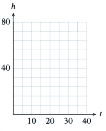
\includegraphics[width=\linewidth]{images/fig-Example2}
\end{sbspanel}%
\end{sidebyside}%
\par
%
\begin{enumerate}[label=\alph*]
\item{}Write an equation for the height of the seedlings in terms of the number of days since they were planted.%
\item{}Graph the equation.%
\end{enumerate}
%
\par\smallskip%
\noindent\textbf{\blocktitlefont Answer}.\quad{}%
\begin{multicols}{2}
\begin{enumerate}[label=\alph*]
\item{}\(h = 6 + 2t\)%
\item{}\begin{sidebyside}{1}{0}{0.25}{0}%
\begin{sbspanel}{0.5}%
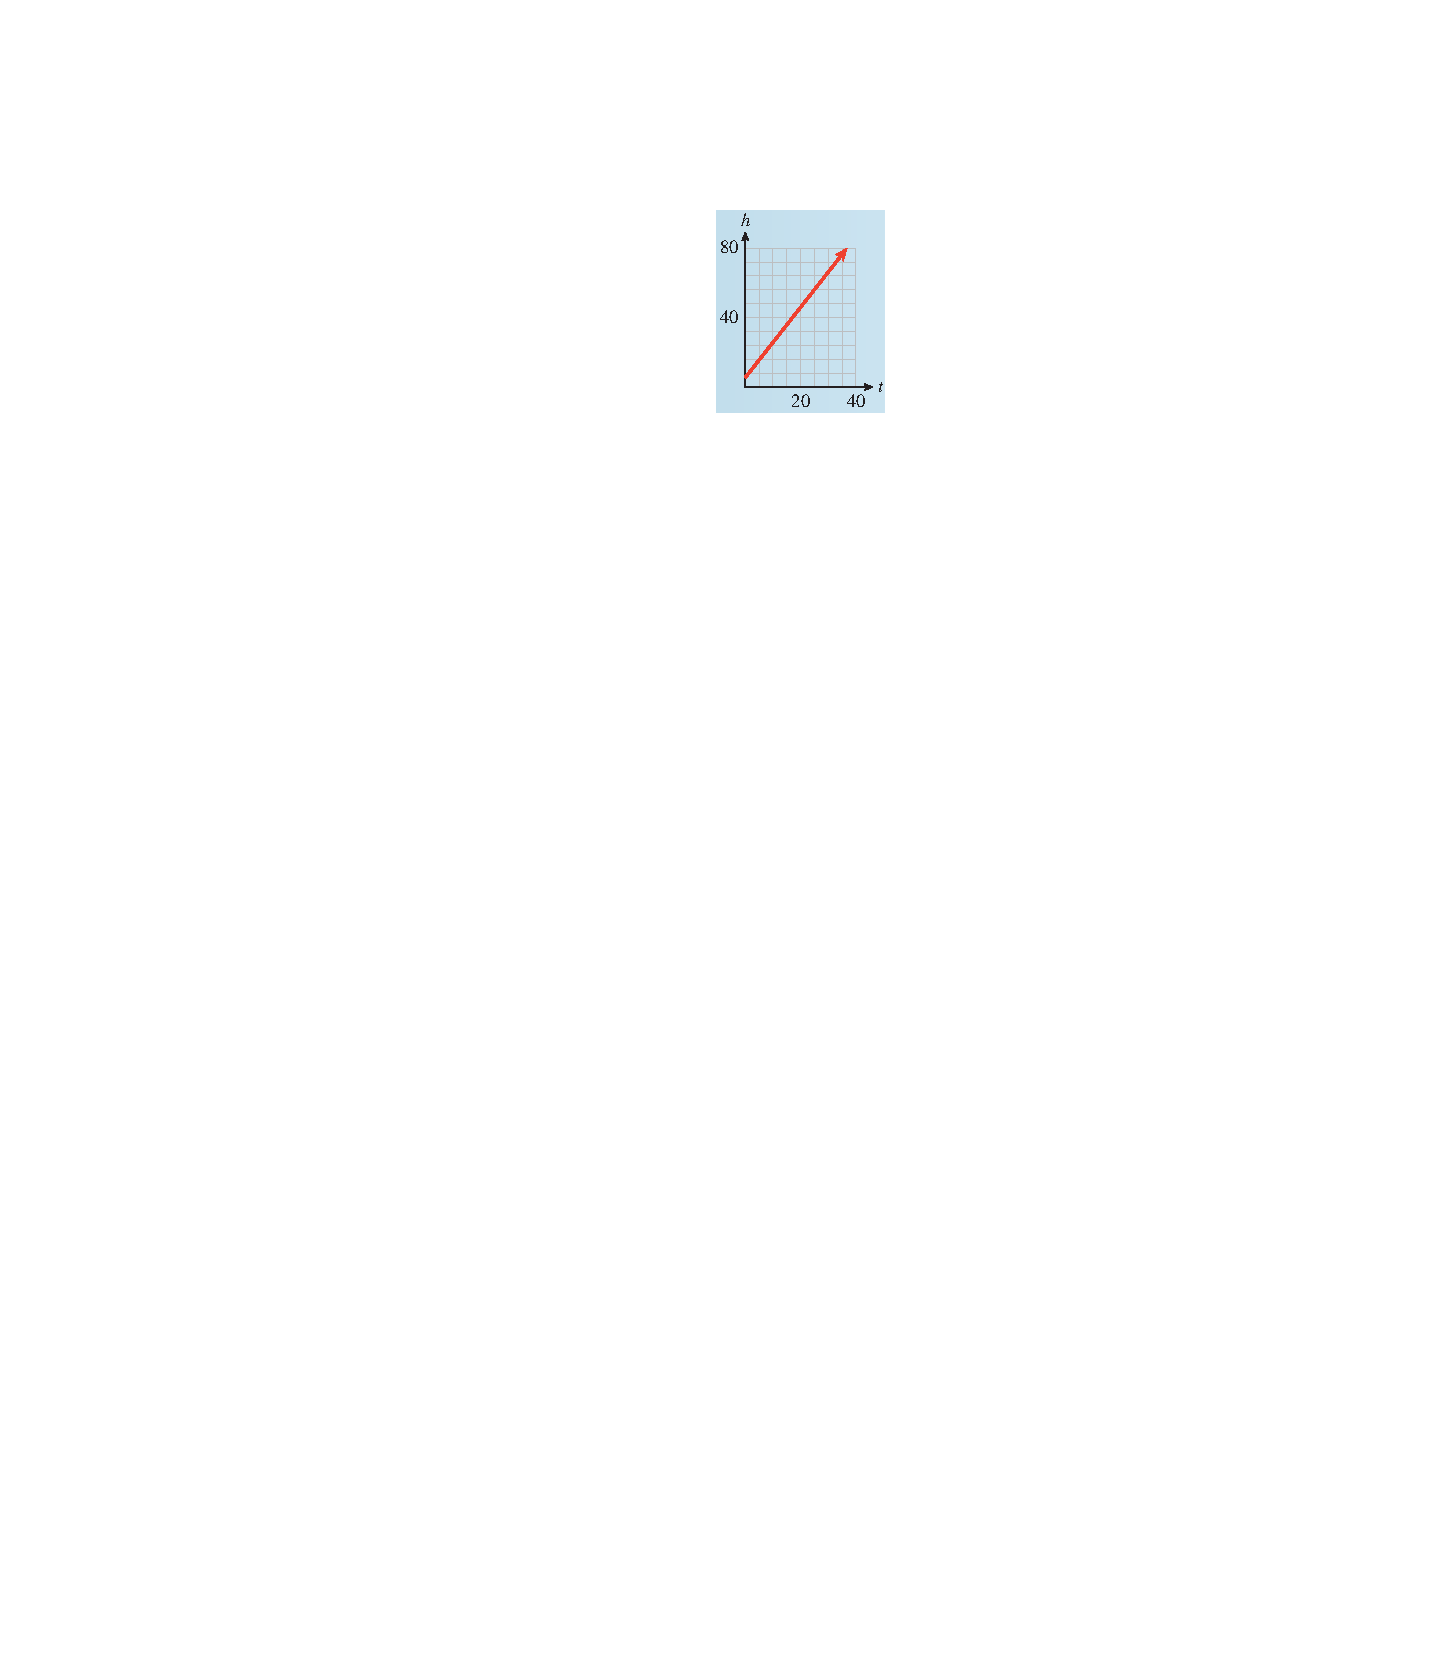
\includegraphics[width=\linewidth]{images/fig-in-ex-ans-1-1-1}
\end{sbspanel}%
\end{sidebyside}%
%
\end{enumerate}
\end{multicols}
%
\end{inlineexercisesolution}
\begin{inlineexercisesolution}{1.1.5}{}{g:exercise:idm93578406752}
Use your equation from Checkpoint~1.1.4 to answer the questions.  Illustrate each answer on the graph.%
%
\begin{enumerate}[label=\alph*]
\item{}How tall is the corn after 3 weeks?%
\item{}How long will it be before the corn is 6 feet tall?%
\end{enumerate}
\par\smallskip%
\noindent\textbf{\blocktitlefont Hint}.\quad{}For part (b), convert feet to inches.%
\par\smallskip%
\noindent\textbf{\blocktitlefont Answer}.\quad{}%
\begin{multicols}{2}
\begin{enumerate}[label=\alph*]
\item{}\(48\) inches tall%
\item{}\(33\) days%
\end{enumerate}
\end{multicols}
%
\end{inlineexercisesolution}
\subsection*{1.1.2 Choosing Scales for the Axes}
\addcontentsline{toc}{subsection}{1.1.2 Choosing Scales for the Axes}
\begin{inlineexercisesolution}{1.1.8}{}{x:exercise:exercise-Silver-Lake}
Silver Lake has been polluted by industrial waste products.  The concentration of toxic chemicals in the water is currently 285 parts per million (ppm).  Environmental officials would like to reduce the concentration by 15 ppm each year.%
\begin{enumerate}[label=\alph*]
\item{}Complete the table of values showing the desired concentration, \(C,\)~ of toxic chemicals \(t\) years from now.  For each \(t\)-value, calculate the corresponding value for \(C\).  Write your answers as ordered pairs.%
\begin{sidebyside}{1}{0}{0}{0}%
\begin{sbspanel}{1}%
{\centering%
{\tabularfont%
\begin{tabular}{AcAcAcAcA}\hrulethick
\(t\)&\(C\)&&\((t,C)\)\tabularnewline\hrulethin
\(0\)&&\(C=285-15(\alert{0})\)&\((0, ~~~~ )\)\tabularnewline\hrulethin
\(5\)&&\(C=285-15(\alert{5})\)&\((5, ~~~~ )\)\tabularnewline\hrulethin
\(10\)&&\(C=285-15(\alert{10})\)&\((10, ~~~~ )\)\tabularnewline\hrulethin
\(15\)&&\(C=285-15(\alert{15})\)&\((15, ~~~~ )\)\tabularnewline\hrulethin
\end{tabular}
}%
\par}
\end{sbspanel}%
\end{sidebyside}%
\item{}To choose scales for the axes, notice that the value of \(C\) starts at 285 and decreases from there.  We'll scale the vertical axis up to 300, and use 10 tick marks at intervals of 30.  Graph the ordered pairs on the grid, and connect them with a straight line. Extend the graph until it reaches the horizontal axis, but no farther.  Points with negative \(C\)-coordinates have no meaning for the problem.%
\begin{sidebyside}{1}{0.3}{0.3}{0}%
\begin{sbspanel}{0.4}%
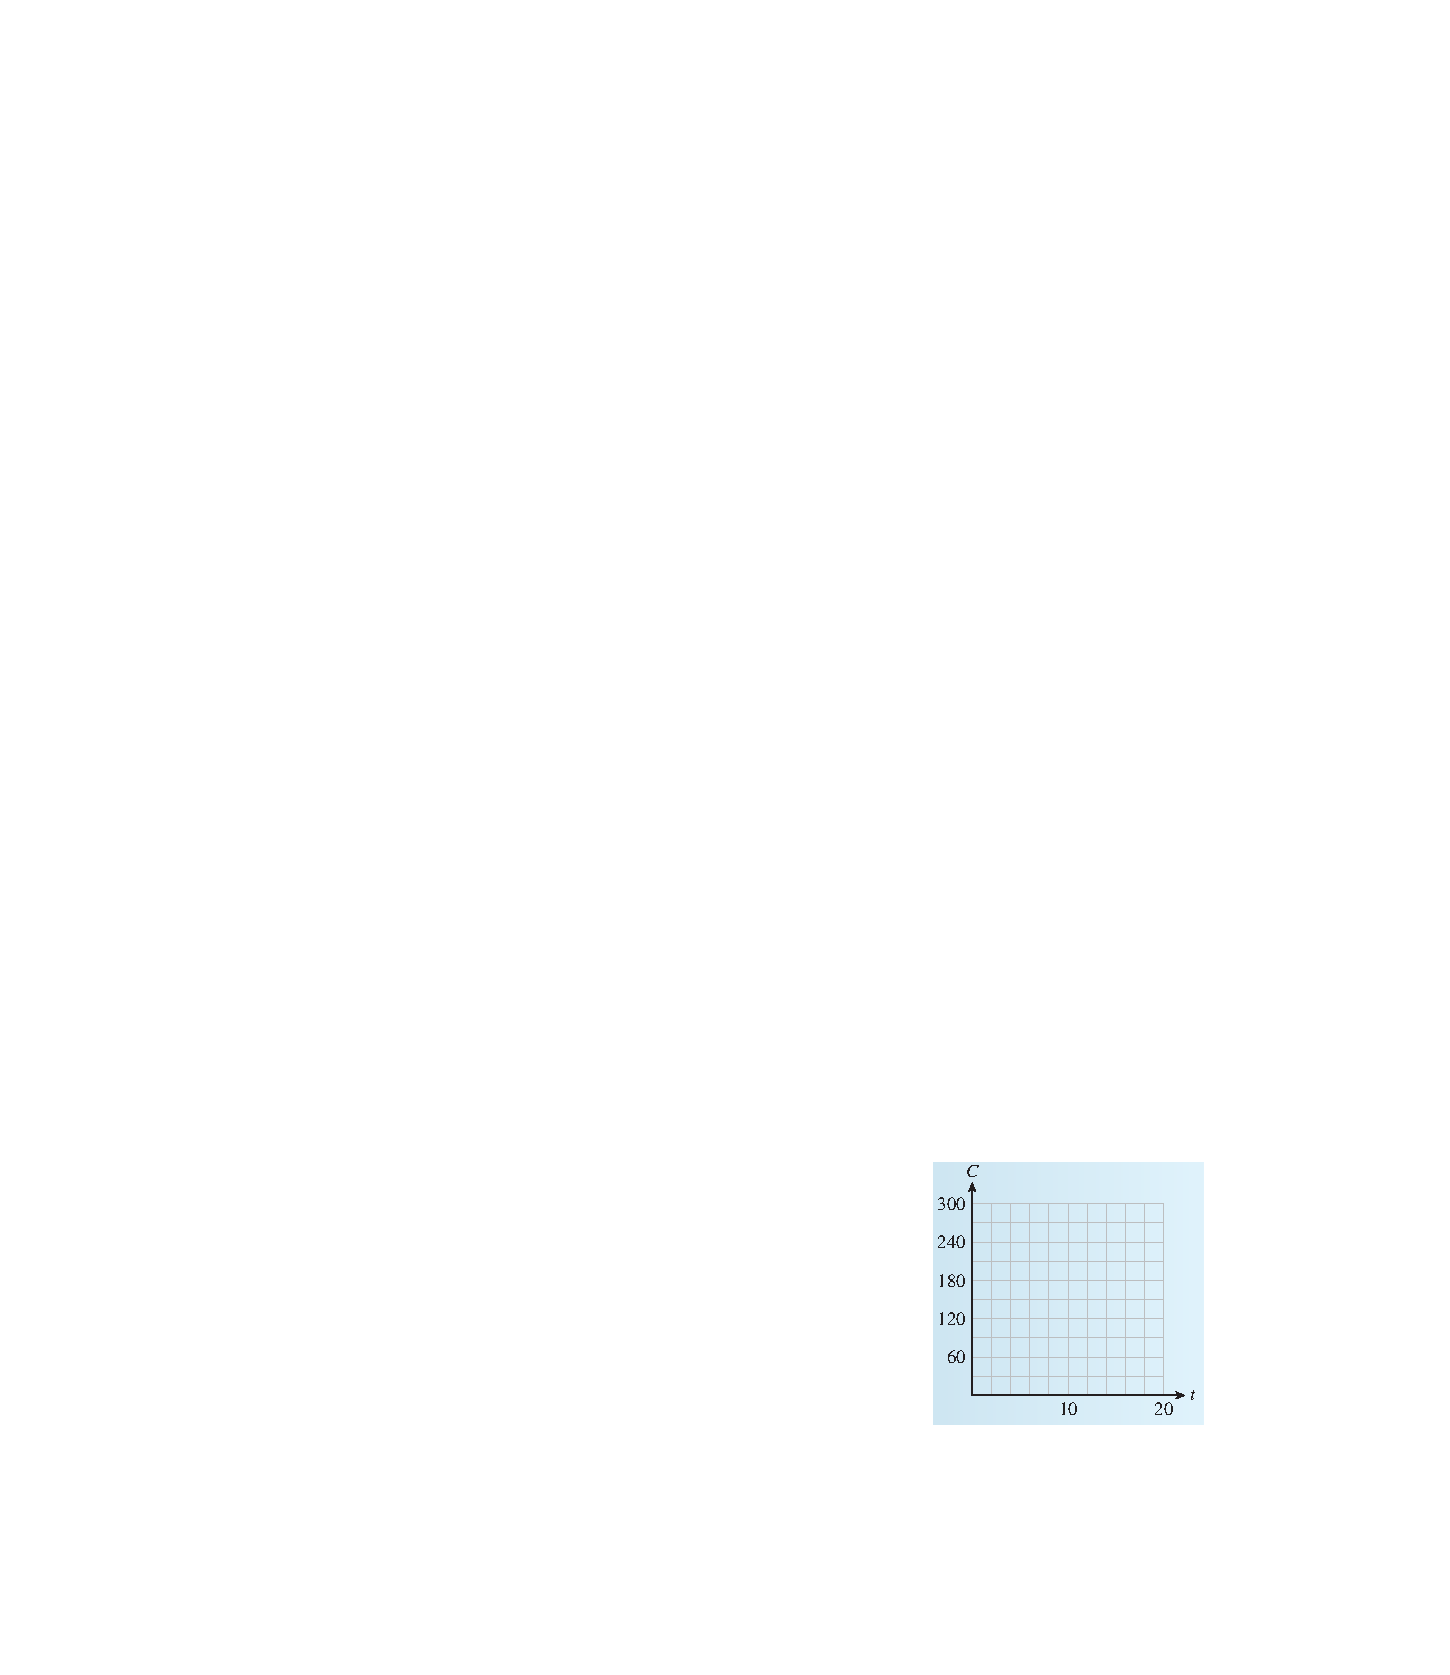
\includegraphics[width=\linewidth]{images/fig-Exercise3}
\end{sbspanel}%
\end{sidebyside}%
\item{}Write an equation for the concentration, \(C\), of toxic chemicals \(t\) years from now.%
\end{enumerate}
%
\par\smallskip%
\noindent\textbf{\blocktitlefont Hint}.\quad{}For part (c): The concentration is initially 285 ppm, and we subtract 15 ppm for each year that passes, or \(15 \times t\).%
\par\smallskip%
\noindent\textbf{\blocktitlefont Answer}.\quad{}%
\begin{multicols}{3}
\begin{enumerate}[label=\alph*]
\item{}\begin{sidebyside}{1}{0}{0}{0}%
\begin{sbspanel}{1}%
{\centering%
{\tabularfont%
\begin{tabular}{AcA}\hrulethick
\((t,C)\)\tabularnewline\hrulethin
\((0,285)\)\tabularnewline\hrulethin
\((5,210)\)\tabularnewline\hrulethin
\((10,135)\)\tabularnewline\hrulethin
\((15,60)\)\tabularnewline\hrulethin
\end{tabular}
}%
\par}
\end{sbspanel}%
\end{sidebyside}%
%
\item{}\begin{sidebyside}{1}{0.125}{0.125}{0}%
\begin{sbspanel}{0.75}%
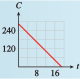
\includegraphics[width=\linewidth]{images/fig-in-ex-ans-1-1-3}
\end{sbspanel}%
\end{sidebyside}%
%
\item{}\(C = 285 - 15t\)%
\end{enumerate}
\end{multicols}
%
\end{inlineexercisesolution}
\begin{inlineexercisesolution}{1.1.11}{}{g:exercise:idm93552731504}
%
\begin{enumerate}[label=\alph*]
\item{}Solve the equation \(2y - 1575 = 45x\) for \(y\) in terms of \(x\).%
\item{}Graph the equation on a graphing calculator. Use the window%
\begin{sidebyside}{1}{0}{0}{0}%
\begin{sbspanel}{1}%
{\centering%
{\tabularfont%
\begin{tabular}{lllll}
Xmin\(=-50\)&&Xmax\(=50\)&&Xscl\(=5\)\tabularnewline[0pt]
Ymin\(=-500\)&&Ymax\(=1000\)&&Yscl\(=100\)
\end{tabular}
}%
\par}
\end{sbspanel}%
\end{sidebyside}%
\item{}Sketch the graph on paper. Use the window settings to choose appropriate scales for the axes.%
\end{enumerate}
%
\par\smallskip%
\noindent\textbf{\blocktitlefont Answer}.\quad{}%
\begin{multicols}{2}
\begin{enumerate}[label=\alph*]
\item{}\(y = (1575 + 45x)/ 2 \)%
\item{}\begin{sidebyside}{1}{0.15}{0.15}{0}%
\begin{sbspanel}{0.7}%
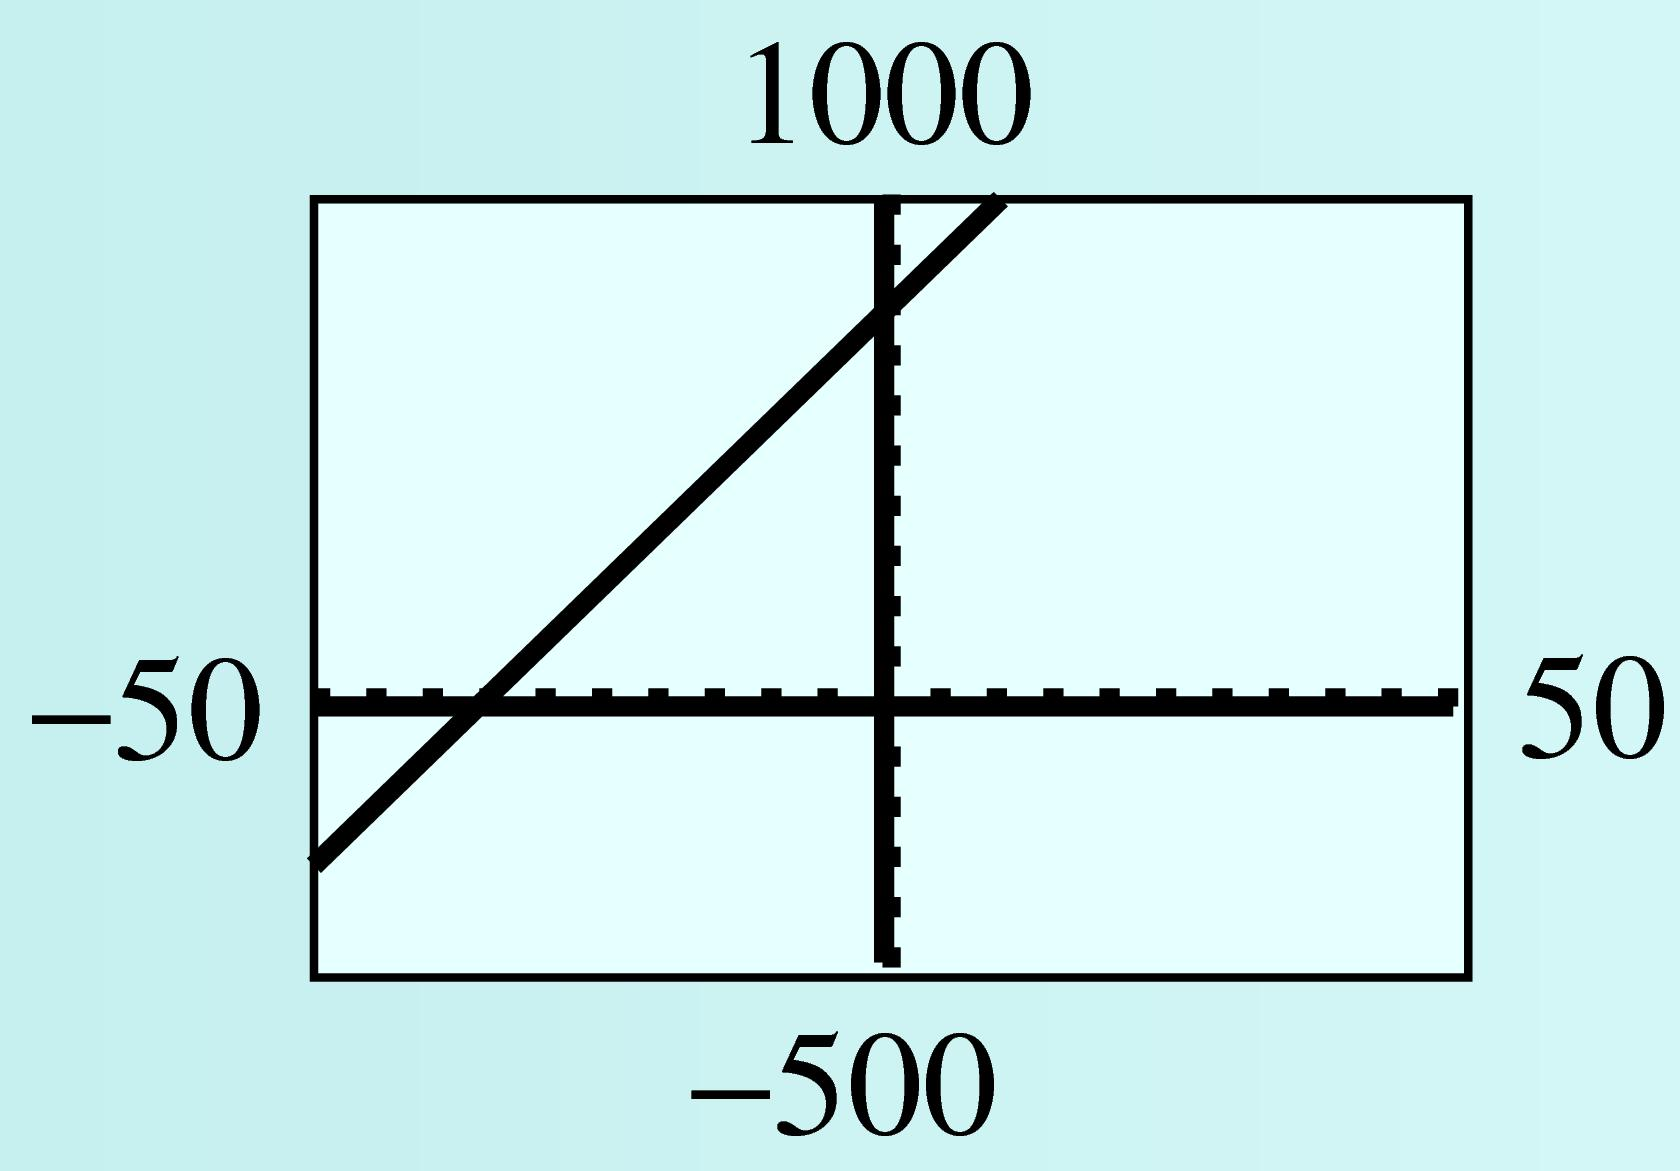
\includegraphics[width=\linewidth]{images/fig-in-ex-ans-1-1-4b.jpg}
\end{sbspanel}%
\end{sidebyside}%
%
\item{}\begin{sidebyside}{1}{0.25}{0.25}{0}%
\begin{sbspanel}{0.5}%
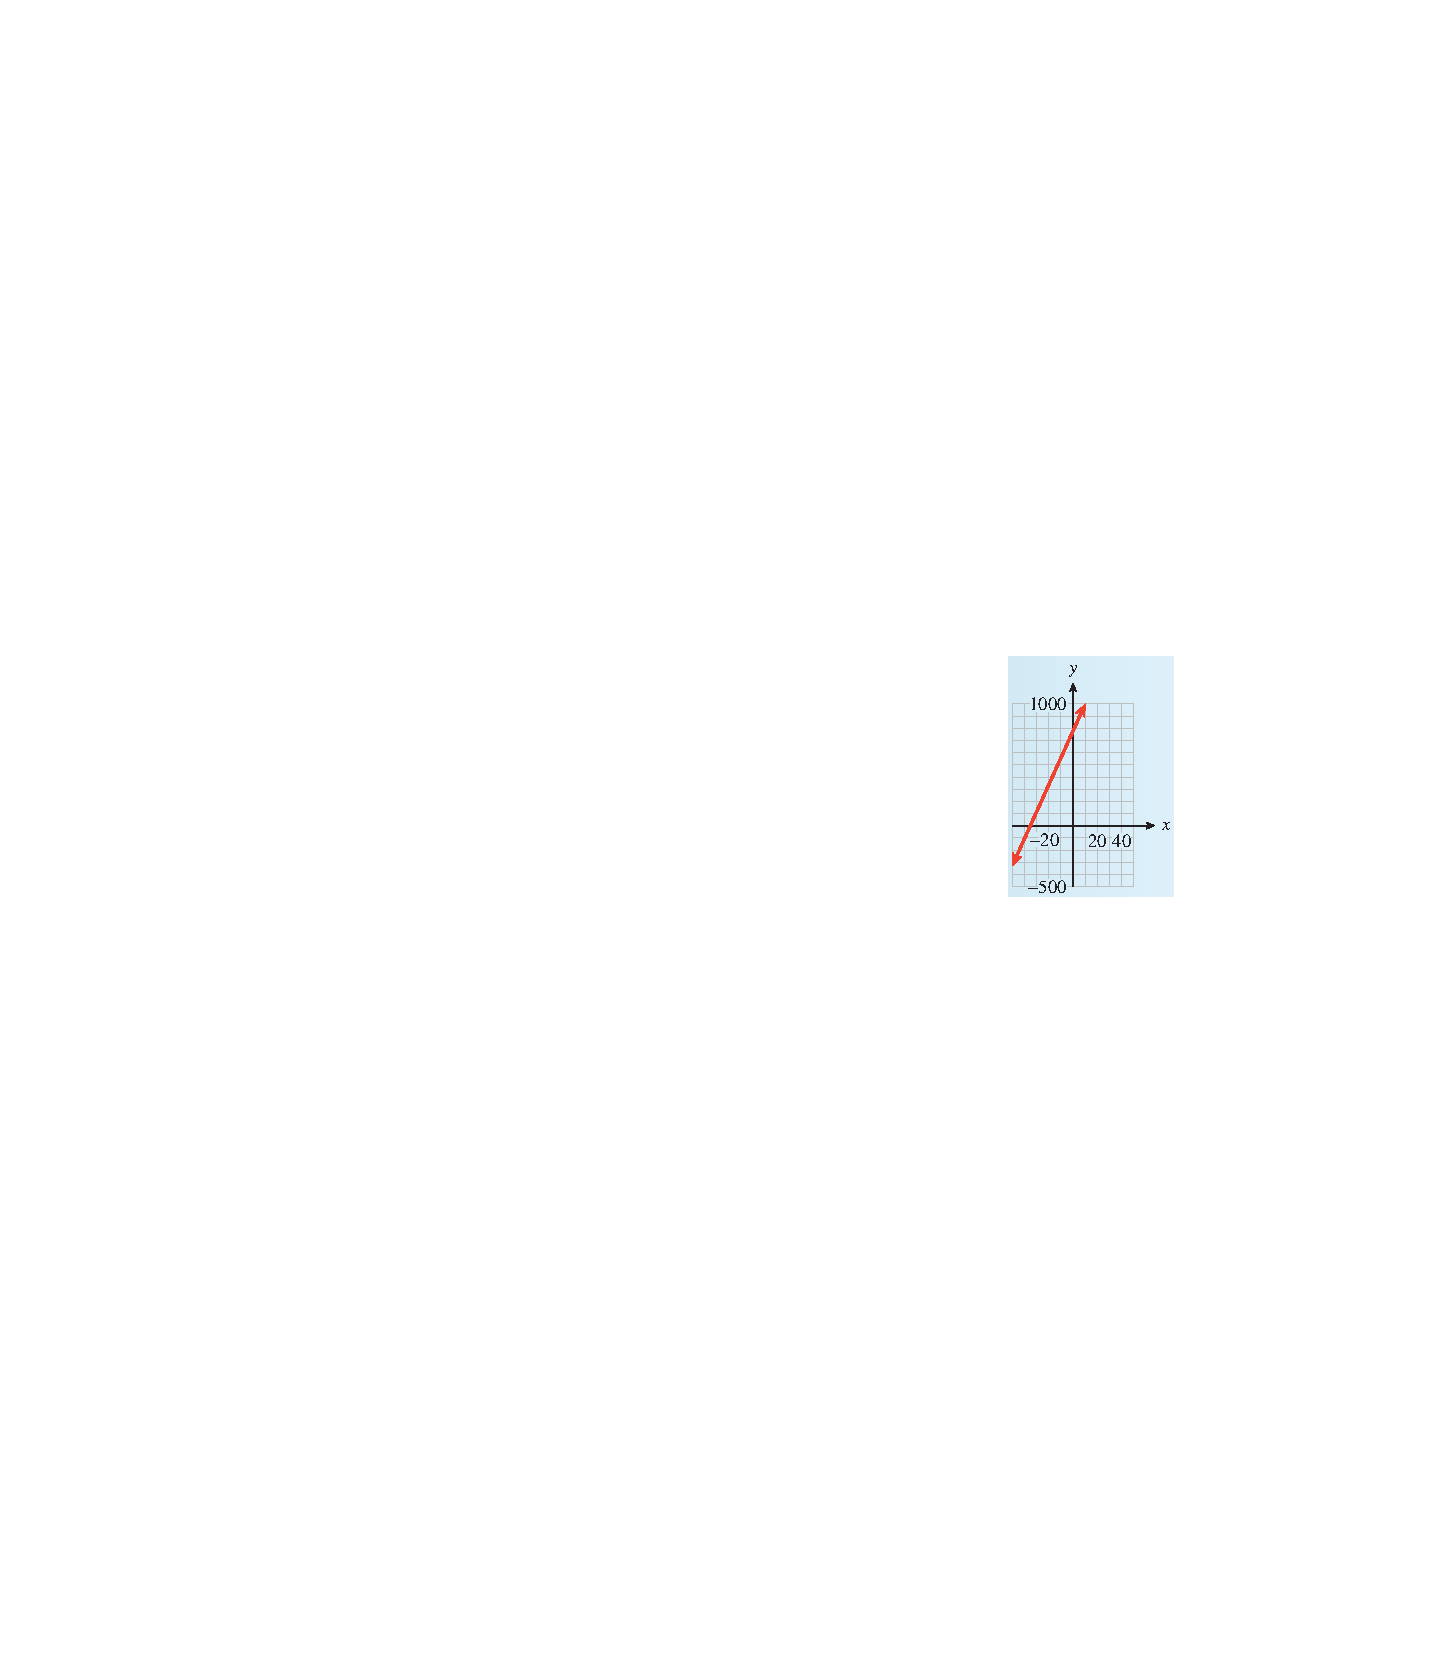
\includegraphics[width=\linewidth]{images/fig-in-ex-ans-1-1-4c}
\end{sbspanel}%
\end{sidebyside}%
%
\end{enumerate}
\end{multicols}
%
\end{inlineexercisesolution}
\subsection*{1.1.3 Linear Equations}
\addcontentsline{toc}{subsection}{1.1.3 Linear Equations}
\begin{inlineexercisesolution}{1.1.13}{}{x:exercise:exercise-crops}
In central Nebraska, each acre of corn requires 25 acre-inches of water per year, and each acre of winter wheat requires 18 acre-inches of water. (An acre-inch is the amount of water needed to cover one acre of land to a depth of one inch.)  A farmer can count on 9000 acre-inches of water for the coming year.  (Source:  Institute of Agriculture and Natural Resources, University of Nebraska)%
\begin{enumerate}[label=\alph*]
\item{}Write an equation relating the number of acres of corn, \(x\), and the number of acres of wheat, \(y\), that the farmer can plant.%
\item{}Complete the table.%
\begin{sidebyside}{1}{0}{0}{0}%
\begin{sbspanel}{1}%
{\centering%
{\tabularfont%
\begin{tabular}{AcAcAcAcAcA}\hrulethick
\(x\)&\(50\)&\(100\)&\(150\)&\(200\)\tabularnewline\hrulethin
\(y\)&\(\hphantom{0000}\)&\(\hphantom{0000}\)&\(\hphantom{0000}\)&\(\hphantom{0000}\)\tabularnewline\hrulethin
\end{tabular}
}%
\par}
\end{sbspanel}%
\end{sidebyside}%
\end{enumerate}
%
\par\smallskip%
\noindent\textbf{\blocktitlefont Answer}.\quad{}%
\begin{enumerate}[label=\alph*]
\item{}\(25x + 18y = 9000\)%
\item{}\begin{sidebyside}{1}{0}{0.55}{0}%
\begin{sbspanel}{0.45}%
{\centering%
{\tabularfont%
\begin{tabular}{AcAcAcAcAcA}\hrulethick
\(x\)&\(50\)&\(100\)&\(150\)&\(200\)\tabularnewline\hrulethin
\(y\)&\(430.6\)&\(361.1\)&\(291.7\)&\(222.2\)\tabularnewline\hrulethin
\end{tabular}
}%
\par}
\end{sbspanel}%
\end{sidebyside}%
%
\end{enumerate}
%
\end{inlineexercisesolution}
\subsection*{1.1.4 Intercepts}
\addcontentsline{toc}{subsection}{1.1.4 Intercepts}
\begin{inlineexercisesolution}{1.1.15}{}{g:exercise:idm93556371216}
%
\begin{enumerate}[label=\alph*]
\item{}Find the intercepts of the graph in Example~1.1.12, about the advertising budget for Albert's Appliances: \(150x + 50y = 3000\).%
\item{}What do the intercepts tell us about the problem?%
\end{enumerate}
\par\smallskip%
\noindent\textbf{\blocktitlefont Answer}.\quad{}\((20, 0)\): The manager can buy \(20\) television ads if she buys no radio ads. \((0, 60)\): The manager can buy \(60\) radio ads if she buys no television ads.%
\end{inlineexercisesolution}
\subsection*{1.1.5 Intercept Method for Graphing Lines}
\addcontentsline{toc}{subsection}{1.1.5 Intercept Method for Graphing Lines}
\begin{inlineexercisesolution}{1.1.17}{}{g:exercise:idm93556340784}
%
\begin{enumerate}[label=\alph*]
\item{}In Checkpoint~1.1.13, you wrote an equation about crops in Nebraska. Find the intercepts of the graph.%
\item{}Use the intercepts to help you choose appropriate scales for the axes, and then graph the equation.%
\item{}What do the intercepts tell us about the problem?%
\end{enumerate}
\par\smallskip%
\noindent\textbf{\blocktitlefont Answer}.\quad{}a., c. \(~~(360, 0)\): If he plants no wheat, the farmer can plant \(360\) acres of corn. \((0, 500)\): If he plants no corn, the farmer can plant 500 acres of wheat.%
\begin{sidebyside}{3}{0}{0}{0.05}%
\begin{sbspanel}{0.05}%
b.%
\end{sbspanel}%
\begin{sbspanel}{0.25}%
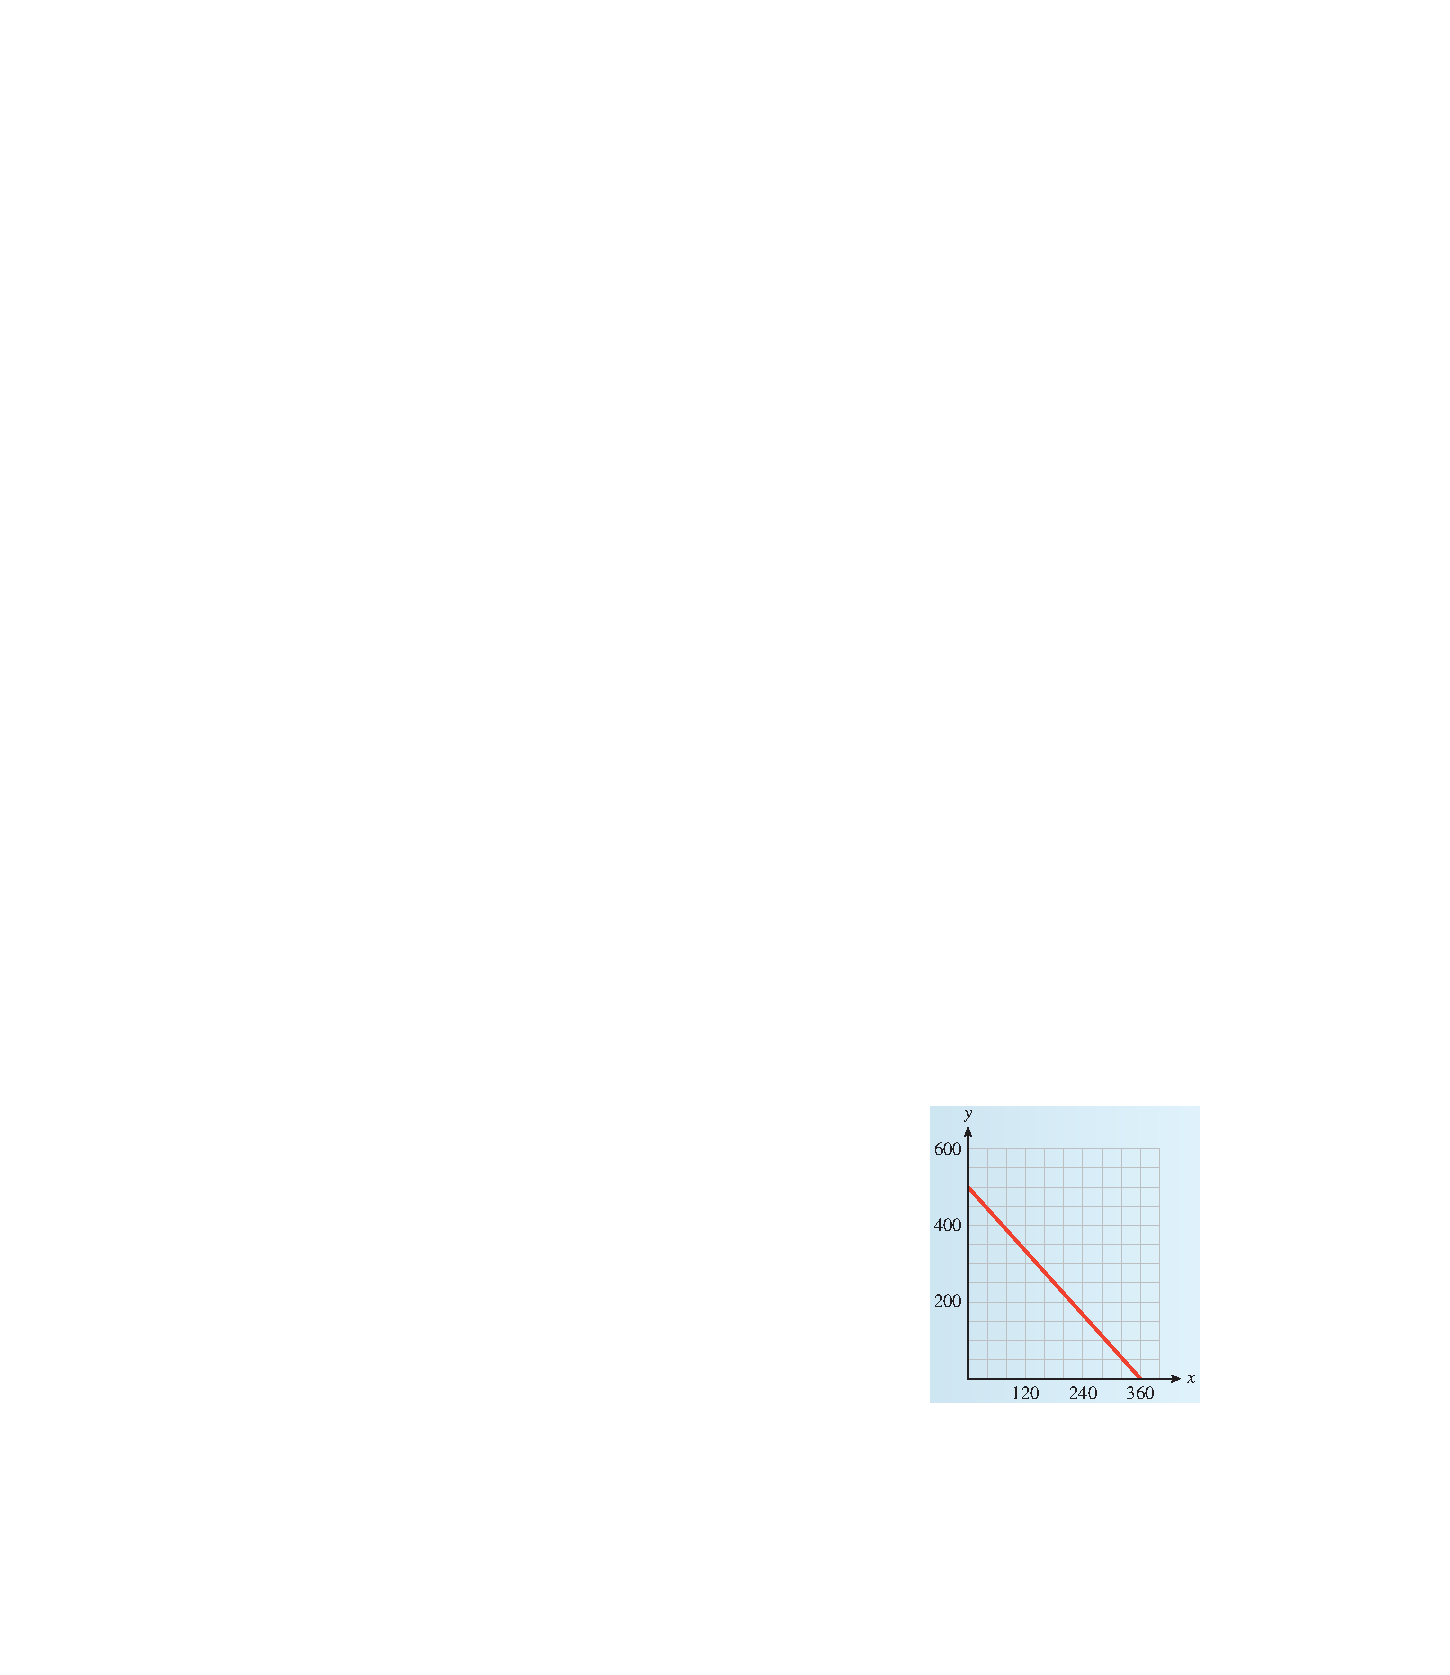
\includegraphics[width=\linewidth]{images/fig-in-ex-ans-1-1-7}
\end{sbspanel}%
\begin{sbspanel}{0.6}%
%
\end{sbspanel}%
\end{sidebyside}%
\end{inlineexercisesolution}
\subsection*{1.1.7 Homework 1.1}
\addcontentsline{toc}{subsection}{1.1.7 Homework 1.1}
\begin{divisionsolution}{1.1.7.1}{}{g:exercise:idm93556283344}%
The temperature in the desert at 6 a.m., just before sunrise, was \(65\degree\)F. The temperature rose \(5\) degrees every hour until it reached its maximum value at about 5 p.m. Complete the table of values for the temperature, \(T\), at \(h\) hours after 6 a.m.%
\begin{sidebyside}{1}{0}{0}{0}%
\begin{sbspanel}{1}%
{\centering%
{\tabularfont%
\begin{tabular}{AcAcAcAcAcAcA}\hrulethick
\(h\)&\(0\)&\(3\)&\(6\)&\(9\)&\(10\)\tabularnewline\hrulethin
\(T\)&\(\hphantom{0000}\)&\(\hphantom{0000}\)&\(\hphantom{0000}\)&\(\hphantom{0000}\)&\(\hphantom{0000}\)\tabularnewline\hrulethin
\end{tabular}
}%
\par}
\end{sbspanel}%
\end{sidebyside}%
\par
%
\begin{enumerate}[label=\alph*]
\item{}Write an equation for the temperature, \(T\), in terms of \(h\).%
\item{}Graph the equation.%
\begin{sidebyside}{1}{0.3}{0.3}{0}%
\begin{sbspanel}{0.4}%
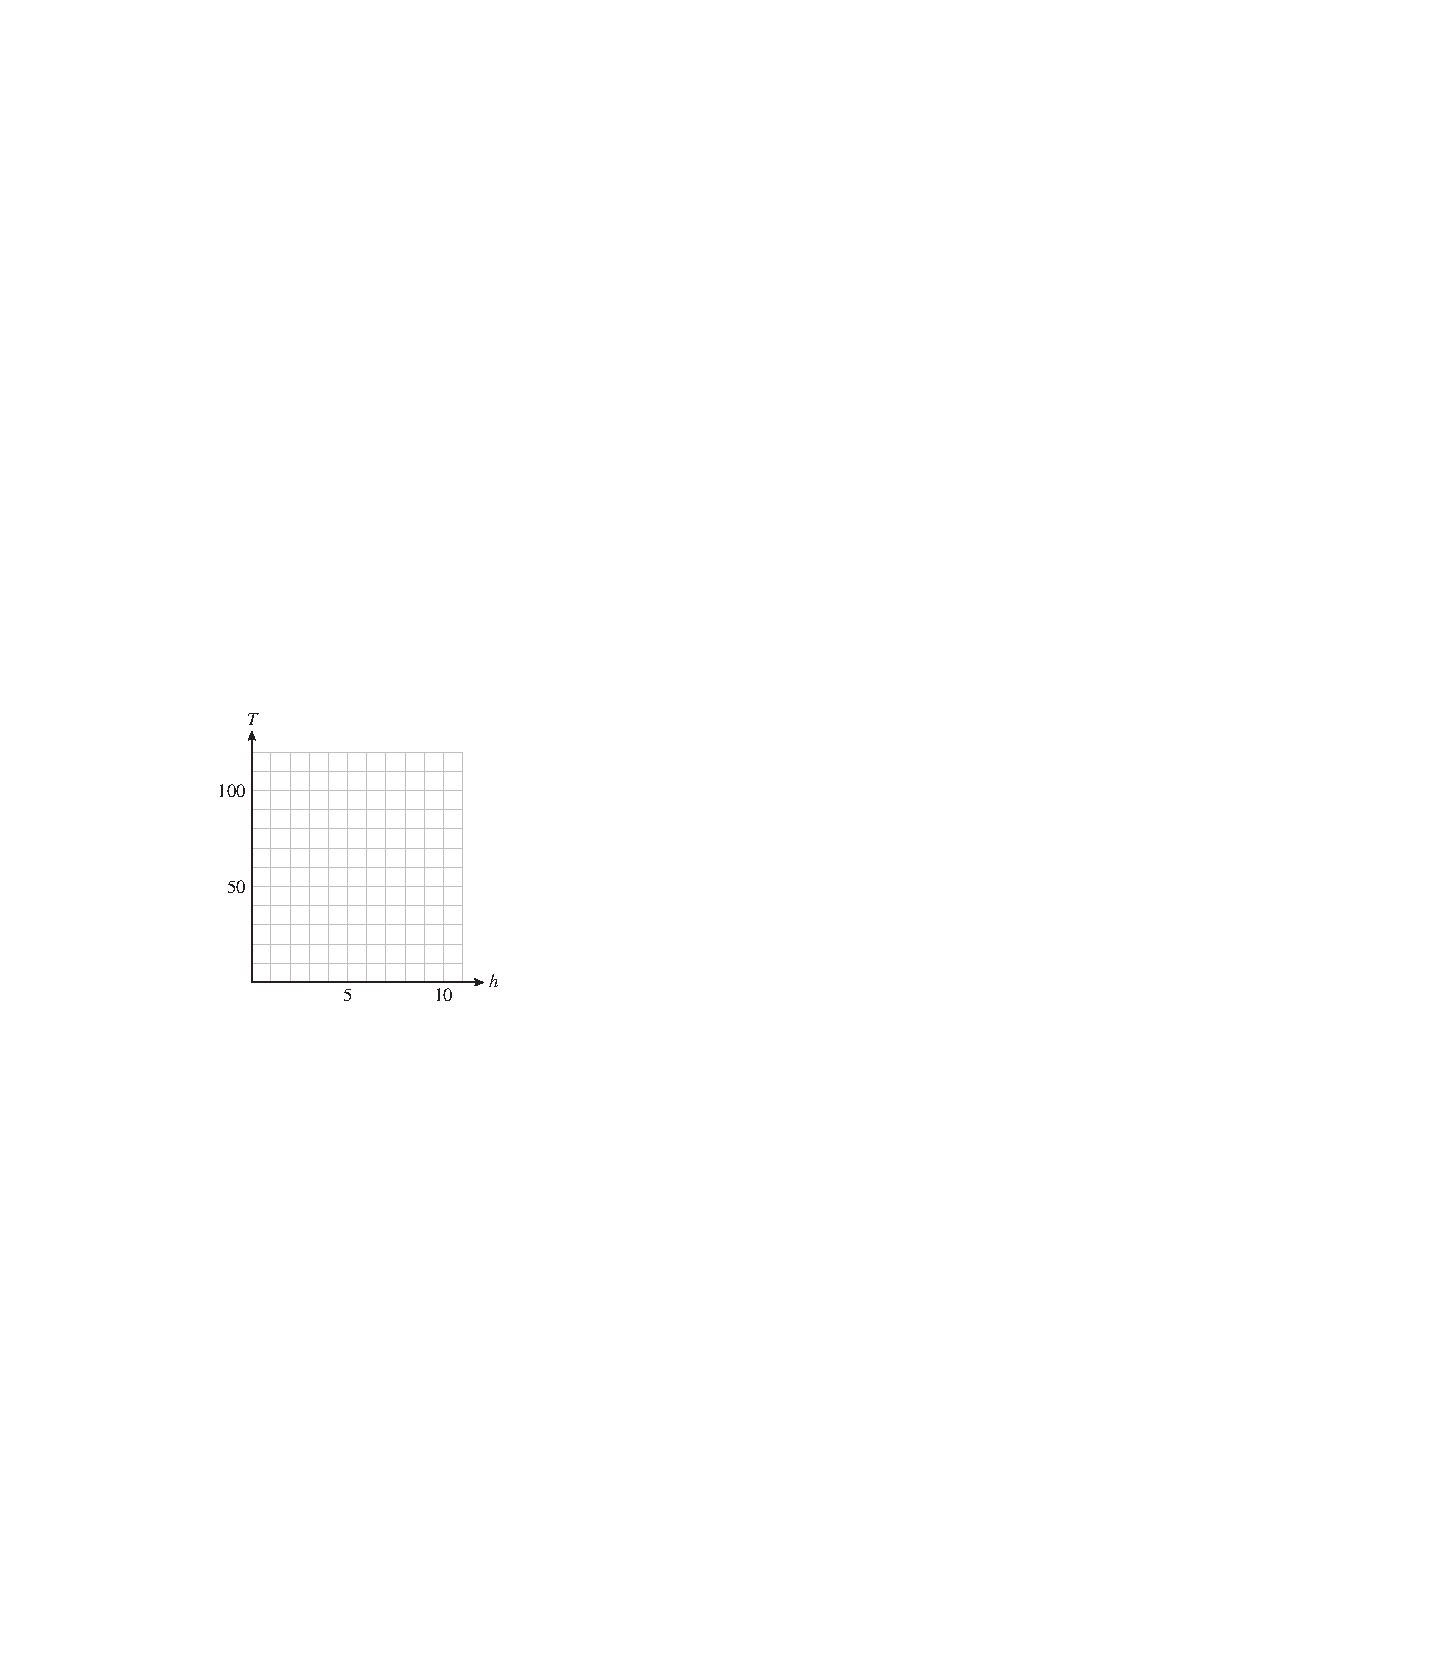
\includegraphics[width=\linewidth]{images/fig-ex-1-1-1}
\end{sbspanel}%
\end{sidebyside}%
\item{}How hot is it at noon? Illustrate the answer on your graph.%
\item{}When will the temperature be \(110\degree\)F? Illustrate the answer on your graph.%
\end{enumerate}
%
\par\smallskip%
\noindent\textbf{\blocktitlefont Answer}.\quad{}\begin{sidebyside}{1}{0}{0}{0}%
\begin{sbspanel}{1}%
{\centering%
{\tabularfont%
\begin{tabular}{AcAcAcAcAcAcA}\hrulethick
\(h\)&\(0\)&\(3\)&\(6\)&\(9\)&\(10\)\tabularnewline\hrulethin
\(T\)&\(65\)&\(80\)&\(95\)&\(110\)&\(115\)\tabularnewline\hrulethin
\end{tabular}
}%
\par}
\end{sbspanel}%
\end{sidebyside}%
\par
%
\begin{enumerate}[label=\alph*]
\item{}\(T=65+5h\)%
\item{}\begin{sidebyside}{1}{0.3}{0.3}{0}%
\begin{sbspanel}{0.4}%
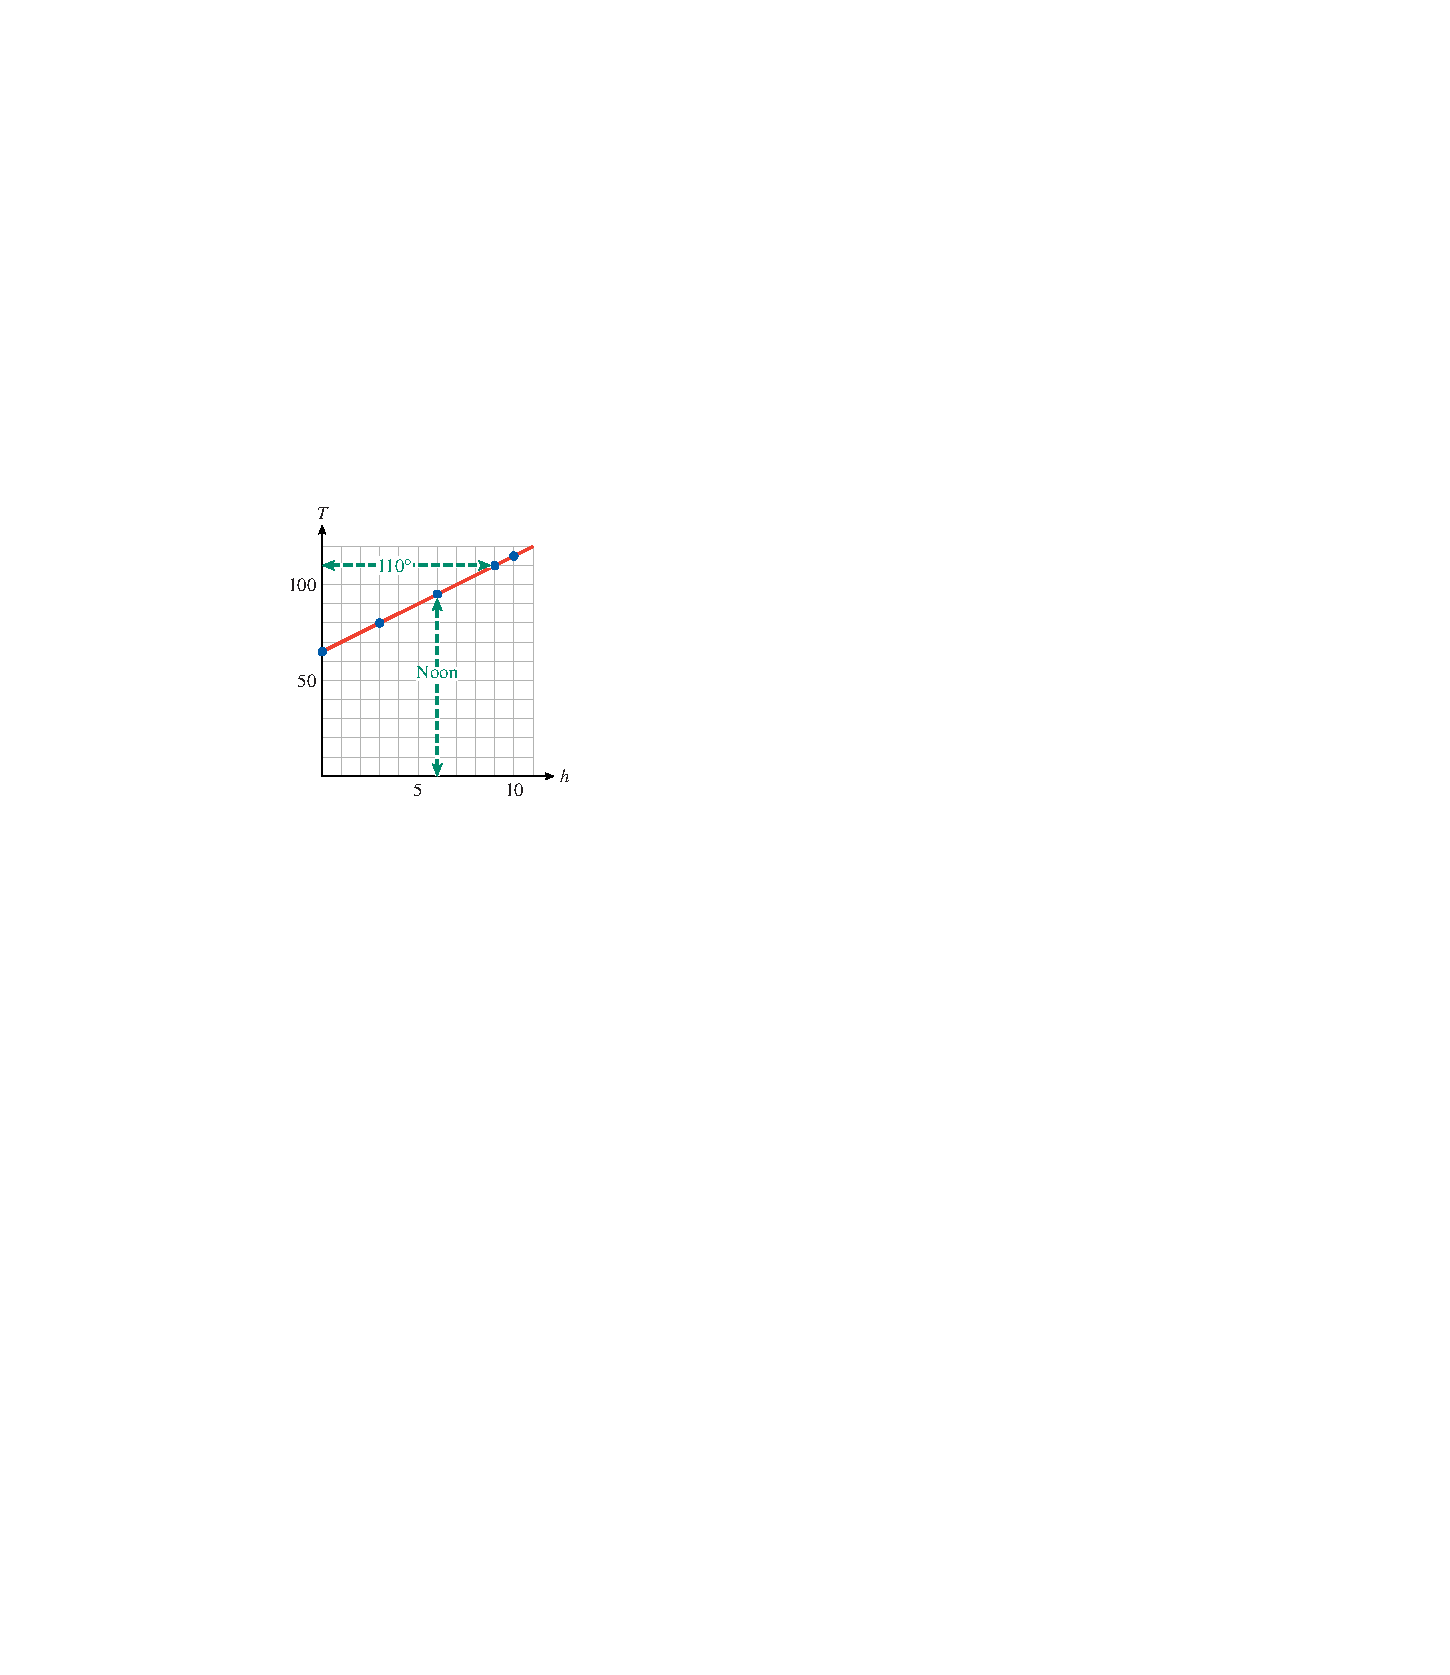
\includegraphics[width=\linewidth]{images/fig-ans-1-1-1}
\end{sbspanel}%
\end{sidebyside}%
%
\item{}\(95\degree\)%
\item{}3 p.m.%
\end{enumerate}
%
\end{divisionsolution}%
\begin{divisionsolution}{1.1.7.2}{}{g:exercise:idm93552419664}%
The taxi out of Dulles Airport charges a traveler with one suitcase an initial fee of \textdollar{}\(2.00\), plus \textdollar{}\(1.50\) for each mile traveled. Complete the table of values showing the charge, \(C\), for a trip of \(n\) miles.%
\begin{sidebyside}{1}{0}{0}{0}%
\begin{sbspanel}{1}%
{\centering%
{\tabularfont%
\begin{tabular}{AcAcAcAcAcAcAcA}\hrulethick
\(n\)&\(0\)&\(5\)&\(10\)&\(15\)&\(20\)&\(25\)\tabularnewline\hrulethin
\(C\)&\(\hphantom{0000}\)&\(\hphantom{0000}\)&\(\hphantom{0000}\)&\(\hphantom{0000}\)&\(\hphantom{0000}\)&\(\hphantom{0000}\)\tabularnewline\hrulethin
\end{tabular}
}%
\par}
\end{sbspanel}%
\end{sidebyside}%
\par
%
\begin{enumerate}[label=\alph*]
\item{}Write an equation for the charge, \(C\), in terms of the number of miles traveled, \(n\).%
\item{}Graph the equation.%
\begin{sidebyside}{1}{0.3}{0.3}{0}%
\begin{sbspanel}{0.4}%
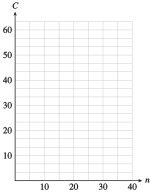
\includegraphics[width=\linewidth]{images/fig-ex-1-1-2}
\end{sbspanel}%
\end{sidebyside}%
\item{}What is the charge for a trip to Mount Vernon,  \(40\) miles from the airport? Illustrate the answer on your graph.%
\item{}If a ride to the National Institutes of Health (NIH) costs \textdollar{}\(39.50\), how far is it from the airport to the NIH? Illustrate the answer on your graph.%
\end{enumerate}
%
\end{divisionsolution}%
\begin{divisionsolution}{1.1.7.3}{}{g:exercise:idm93552398512}%
On October 31, Betty and Paul fill their \(250\)-gallon oil tank for their heater. Beginning in November, they use an average of \(15\) gallons of oil per week. Complete the table of values for the amount of oil, \(A\), left in the tank after \(w\) weeks.%
\begin{sidebyside}{1}{0}{0}{0}%
\begin{sbspanel}{1}%
{\centering%
{\tabularfont%
\begin{tabular}{AcAcAcAcAcAcA}\hrulethick
\(w\)&\(0\)&\(4\)&\(8\)&\(12\)&\(16\)\tabularnewline\hrulethin
\(A\)&\(\hphantom{0000}\)&\(\hphantom{0000}\)&\(\hphantom{0000}\)&\(\hphantom{0000}\)&\(\hphantom{0000}\)\tabularnewline\hrulethin
\end{tabular}
}%
\par}
\end{sbspanel}%
\end{sidebyside}%
\par
%
\begin{enumerate}[label=\alph*]
\item{}Write an equation that expresses the amount of oil, \(A\), in the tank in terms of the number of weeks, \(w\), since October 31.%
\item{}Graph the equation.%
\begin{sidebyside}{1}{0.3}{0.3}{0}%
\begin{sbspanel}{0.4}%
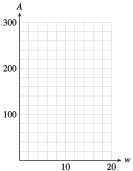
\includegraphics[width=\linewidth]{images/fig-ex-1-1-3}
\end{sbspanel}%
\end{sidebyside}%
\item{}How much did the amount of fuel oil in the tank decrease between the third week and the eighth week? Illustrate this amount on the graph.%
\item{}When will the tank contain more than \(175\) gallons of fuel oil? Illustrate on the graph.%
\end{enumerate}
%
\par\smallskip%
\noindent\textbf{\blocktitlefont Answer}.\quad{}\begin{sidebyside}{1}{0}{0}{0}%
\begin{sbspanel}{1}%
{\centering%
{\tabularfont%
\begin{tabular}{AcAcAcAcAcAcA}\hrulethick
\(w\)&\(0\)&\(4\)&\(8\)&\(12\)&\(16\)\tabularnewline\hrulethin
\(A\)&\(250\)&\(190\)&\(130\)&\(70\)&\(10\)\tabularnewline\hrulethin
\end{tabular}
}%
\par}
\end{sbspanel}%
\end{sidebyside}%
\par
%
\begin{enumerate}[label=\alph*]
\item{}\(A=250-15w\)%
\item{}\begin{sidebyside}{1}{0.25}{0.25}{0}%
\begin{sbspanel}{0.5}%
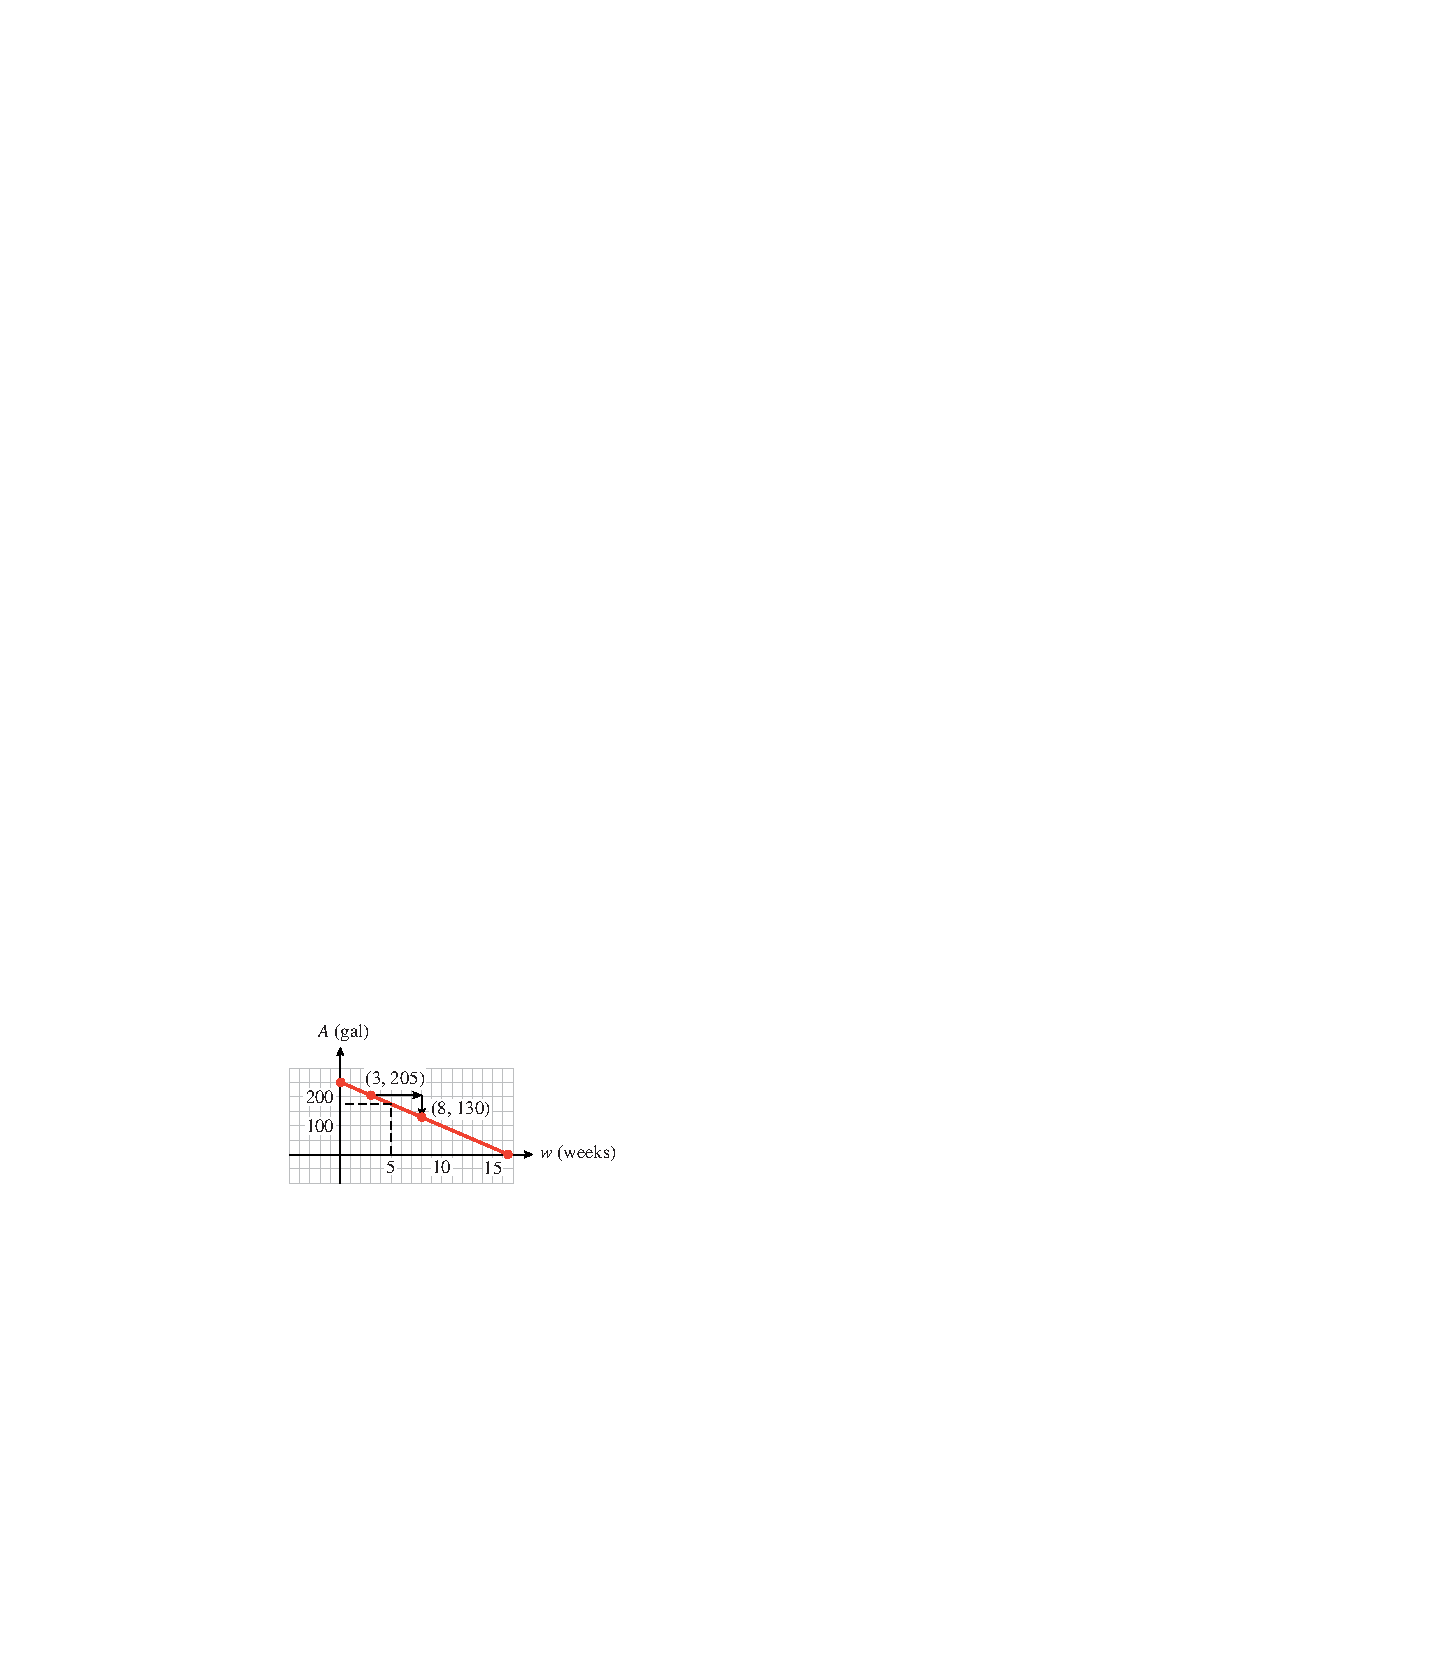
\includegraphics[width=\linewidth]{images/fig-ans-1-1-3}
\end{sbspanel}%
\end{sidebyside}%
%
\item{}75 gallons%
\item{}Until the fifth week%
\end{enumerate}
%
\end{divisionsolution}%
\begin{divisionsolution}{1.1.7.4}{}{g:exercise:idm93552364384}%
Leon's camper has a \(20\)-gallon gas tank, and he gets \(12\) miles to the gallon. (That is, he uses \(\frac{1}{12}\) gallon per mile.) Complete the table of values for the amount of gas, \(g\), left in Leon's tank after driving \(m\) miles.%
\begin{sidebyside}{1}{0}{0}{0}%
\begin{sbspanel}{1}%
{\centering%
{\tabularfont%
\begin{tabular}{AcAcAcAcAcAcA}\hrulethick
\(m\)&\(0\)&\(48\)&\(96\)&\(144\)&\(192\)\tabularnewline\hrulethin
\(g\)&\(\hphantom{0000}\)&\(\hphantom{0000}\)&\(\hphantom{0000}\)&\(\hphantom{0000}\)&\(\hphantom{0000}\)\tabularnewline\hrulethin
\end{tabular}
}%
\par}
\end{sbspanel}%
\end{sidebyside}%
\par
%
\begin{enumerate}[label=\alph*]
\item{}Write an equation that expresses the amount of gas, \(g\), in Leon's fuel tank in terms of the number of miles, \(m\), he has driven.%
\item{}Graph the equation.%
\begin{sidebyside}{1}{0.3}{0.3}{0}%
\begin{sbspanel}{0.4}%
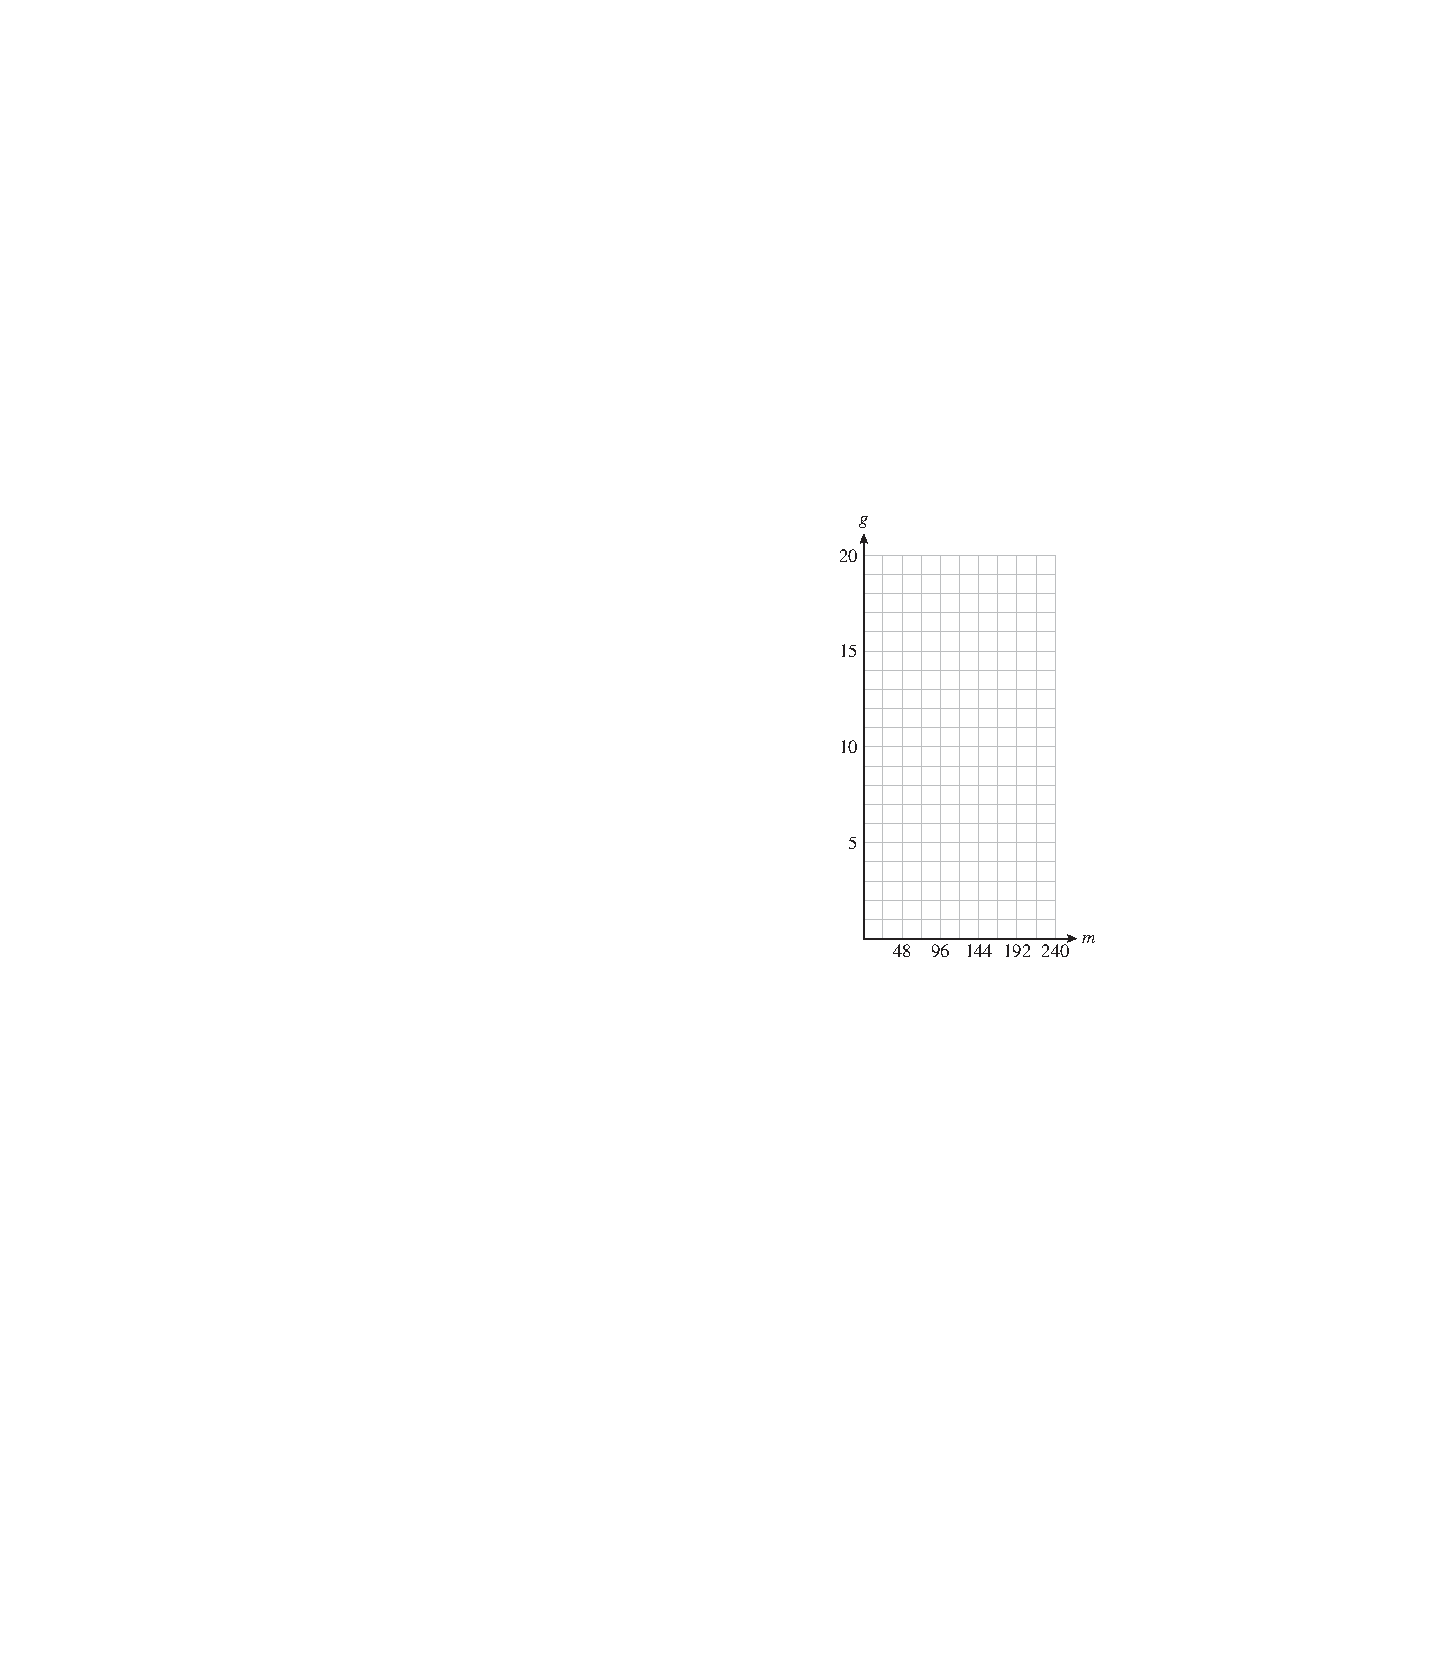
\includegraphics[width=\linewidth]{images/fig-ex-1-1-4}
\end{sbspanel}%
\end{sidebyside}%
\item{}How much gas will Leon use between 8 a.m., when his odometer reads \(96\) miles, and 9 a.m., when the odometer reads \(144\) miles? Illustrate on the graph.%
\item{}If Leon has less than \(5\) gallons of gas left, how many miles has he driven? Illustrate on the graph.%
\end{enumerate}
%
\end{divisionsolution}%
\begin{divisionsolution}{1.1.7.5}{}{g:exercise:idm93552343776}%
Phil and Ernie buy a used photocopier for \textdollar{}\(800\) and set up a copy service on their campus. For each hour that the copier runs, Phil and Ernie make \textdollar{}\(40\).%
\begin{enumerate}[label=\alph*]
\item{}Write an equation that expresses Phil and Ernie's profit (or loss), \(P\), in terms of the number of hours, \(t\), they run the copier.%
\item{}Find the intercepts and sketch the graph. (Suggestion: Scale the horizontal axis from \(0\) to \(40\) in increments of \(5\), and scale the vertical axis from \(-1000\) to \(400\) in increments of \(100\).)%
\item{}What do the intercepts tell us about the profit?%
\end{enumerate}
%
\par\smallskip%
\noindent\textbf{\blocktitlefont Answer}.\quad{}%
\begin{enumerate}[label=\alph*]
\item{}\(P=-800+40t\)%
\item{}\((0,-800)\), \((20,0)\)%
\begin{sidebyside}{1}{0.25}{0.25}{0}%
\begin{sbspanel}{0.5}%
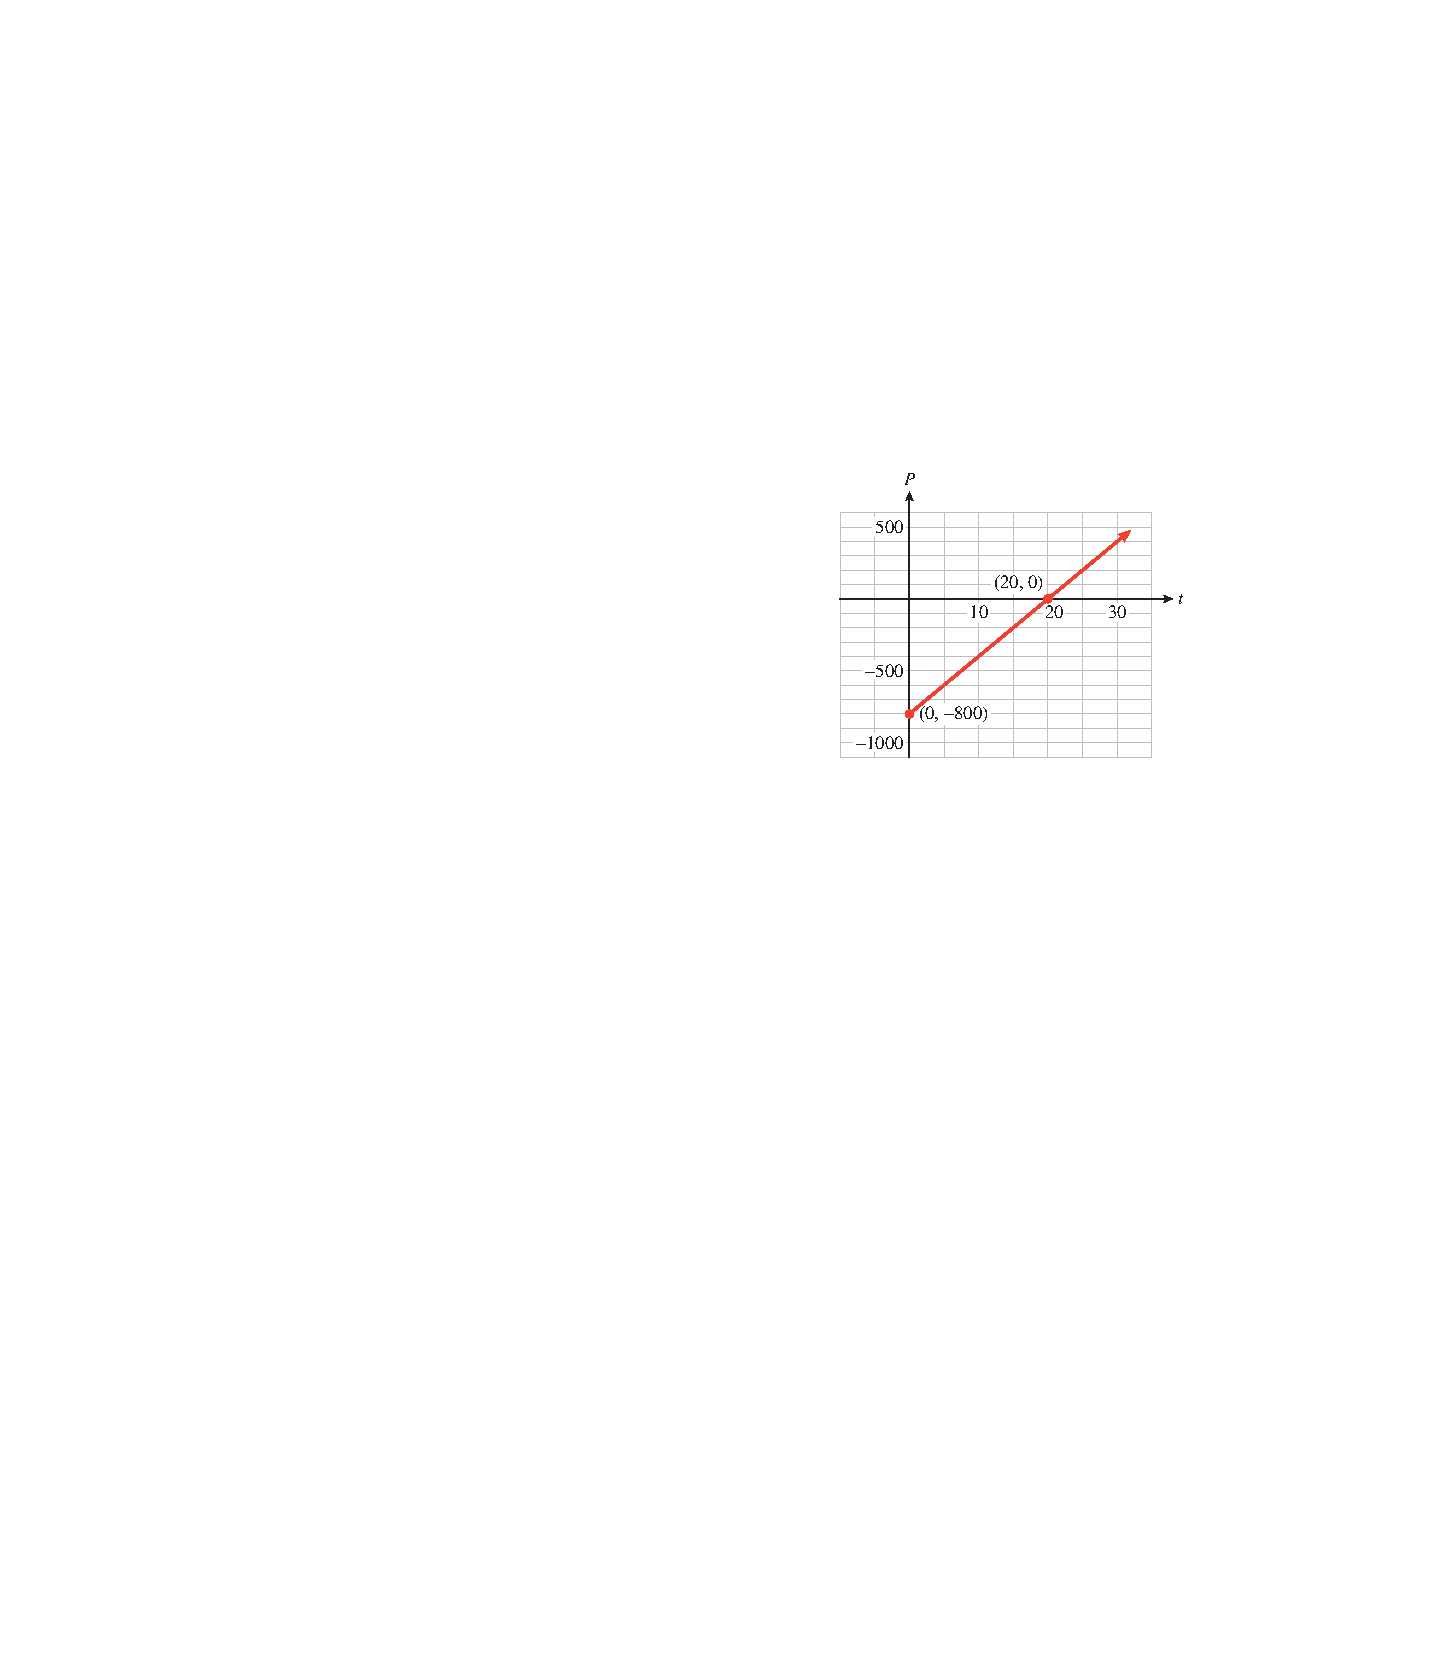
\includegraphics[width=\linewidth]{images/fig-ans-1-1-5}
\end{sbspanel}%
\end{sidebyside}%
\item{}The \(P\)-intercept, \(-800\), is the initial \((t = 0)\) value of the profit. Phil and Ernie start out \(\$800\) in debt. The \(t\)-intercept, \(20\), is the number of hours required for Phil and Ernie to break even.%
\end{enumerate}
%
\end{divisionsolution}%
\begin{divisionsolution}{1.1.7.6}{}{g:exercise:idm93552328256}%
A deep-sea diver is taking some readings at a depth of \(400\) feet. He begins rising at \(20\) feet per minute.%
\begin{enumerate}[label=\alph*]
\item{}Write an equation that expresses the diver’s altitude, \(h\), in terms of the number of minutes, \(m\), elapsed. (Consider a depth of \(400\) feet as an altitude of \(-400\) feet.)%
\item{}Find the intercepts and sketch the graph. (Suggestion: Scale the horizontal axis from \(0\) to \(24\) in increments of \(2\), and scale the vertical axis from \(-500\) to \(100\) in increments of \(50\).)%
\item{}What do the intercepts tell us about the diver's depth?%
\end{enumerate}
%
\end{divisionsolution}%
\begin{divisionsolution}{1.1.7.7}{}{g:exercise:idm93552319616}%
There are many formulas for estimating the annual cost of driving. The Automobile Club estimates that fixed costs for a small car—including insurance, registration, depreciation, and financing—total about \textdollar{}\(5000\) per year. The operating costs for gasoline, oil, maintenance, tires, and so forth are about \(12.5\) cents per mile. (Source: Automobile Association of America)%
\begin{enumerate}[label=\alph*]
\item{}Write an equation for the annual driving cost, \(C\), in terms of \(d\), the number of miles driven.%
\item{}Complete the table of values.%
\begin{sidebyside}{1}{0}{0}{0}%
\begin{sbspanel}{1}%
{\centering%
{\tabularfont%
\begin{tabular}{AlAcAcAcAcAcA}\hrulethick
Miles Driven&\(4000\)&\(8000\)&\(12,000\)&\(16,000\)&\(20,000\)\tabularnewline\hrulethin
Cost (\textdollar{})&\(\hphantom{0000}\)&\(\hphantom{0000}\)&\(\hphantom{0000}\)&\(\hphantom{0000}\)&\(\hphantom{0000}\)\tabularnewline\hrulethin
\end{tabular}
}%
\par}
\end{sbspanel}%
\end{sidebyside}%
\item{}Choose scales for the axes and graph the equation.%
\item{}How much does the annual cost of driving increase when the mileage increases from \(8000\) to \(12,000\) miles? Illustrate this amount on the graph.%
\item{}How much mileage will cause the annual cost to exceed \textdollar{}\(7000\)? Illustrate on the graph.%
\end{enumerate}
%
\par\smallskip%
\noindent\textbf{\blocktitlefont Answer}.\quad{}%
\begin{enumerate}[label=\alph*]
\item{}\(C=5000+0.125d\)%
\item{}Complete the table of values.%
\begin{sidebyside}{1}{0}{0}{0}%
\begin{sbspanel}{1}%
{\centering%
{\tabularfont%
\begin{tabular}{AlAcAcAcAcAcA}\hrulethick
Miles Driven&\(4000\)&\(8000\)&\(12,000\)&\(16,000\)&\(20,000\)\tabularnewline\hrulethin
Cost (\textdollar{})&\(5500\)&\(6000\)&\(6500\)&\(7000\)&\(7500\)\tabularnewline\hrulethin
\end{tabular}
}%
\par}
\end{sbspanel}%
\end{sidebyside}%
\item{}\begin{sidebyside}{1}{0.3}{0.3}{0}%
\begin{sbspanel}{0.4}%
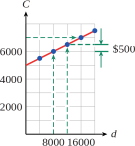
\includegraphics[width=\linewidth]{images/fig-ans-1-1-7}
\end{sbspanel}%
\end{sidebyside}%
%
\item{}\textdollar{}\(500\)%
\item{}More than 16,000 miles%
\end{enumerate}
%
\end{divisionsolution}%
\begin{divisionsolution}{1.1.7.8}{}{g:exercise:idm93552279360}%
The boiling point of water changes with altitude. At sea level, water boils at \(212\degree\)F, and the boiling point diminishes by approximately \(0.002\degree\)F for each \(1\)-foot increase in altitude.%
\begin{enumerate}[label=\alph*]
\item{}Write an equation for the boiling point, \(B\), in terms of \(a\), the altitude in feet.%
\item{}Complete the table of values.%
\begin{sidebyside}{1}{0}{0}{0}%
\begin{sbspanel}{1}%
{\centering%
{\tabularfont%
\begin{tabular}{AlAcAcAcAcAcAcAcA}\hrulethick
Altitude (ft)&\(-500\)&\(0\)&\(1000\)&\(2000\)&\(3000\)&\(4000\)&\(5000\)\tabularnewline\hrulethin
Boiling point (\(\degree\)F)&\(\hphantom{0000}\)&\(\hphantom{0000}\)&\(\hphantom{0000}\)&\(\hphantom{0000}\)&\(\hphantom{0000}\)&\(\hphantom{0000}\)&\(\hphantom{0000}\)\tabularnewline\hrulethin
\end{tabular}
}%
\par}
\end{sbspanel}%
\end{sidebyside}%
\item{}Choose scales for the axes and graph the equation.%
\item{}How much does the boiling point decrease when the altitude increases from \(1000\) to \(3000\) feet? Illustrate this amount on the graph.%
\item{}At what altitudes is the boiling point less than \(204\degree\)F? Illustrate on the graph.%
\end{enumerate}
%
\end{divisionsolution}%
For each table, choose appropriate scales for the axes and plot the given points.%
\begin{exercisegroupcol}{2}
\begin{divisionsolutionegcol}{1.1.7.9}{}{g:exercise:idm93552252432}%
\begin{sidebyside}{1}{0}{0}{0}%
\begin{sbspanel}{1}%
{\centering%
{\tabularfont%
\begin{tabular}{AlAcAcAcAcA}\hrulethick
\(x\)&\(0\)&\(80\)&\(90\)&\(120\)\tabularnewline\hrulethin
\(y\)&\(6\)&\(2\)&\(1.5\)&\(1\)\tabularnewline\hrulethin
\end{tabular}
}%
\par}
\end{sbspanel}%
\end{sidebyside}%
\par\smallskip%
\noindent\textbf{\blocktitlefont Answer}.\quad{}\begin{sidebyside}{1}{0.2}{0.2}{0}%
\begin{sbspanel}{0.6}%
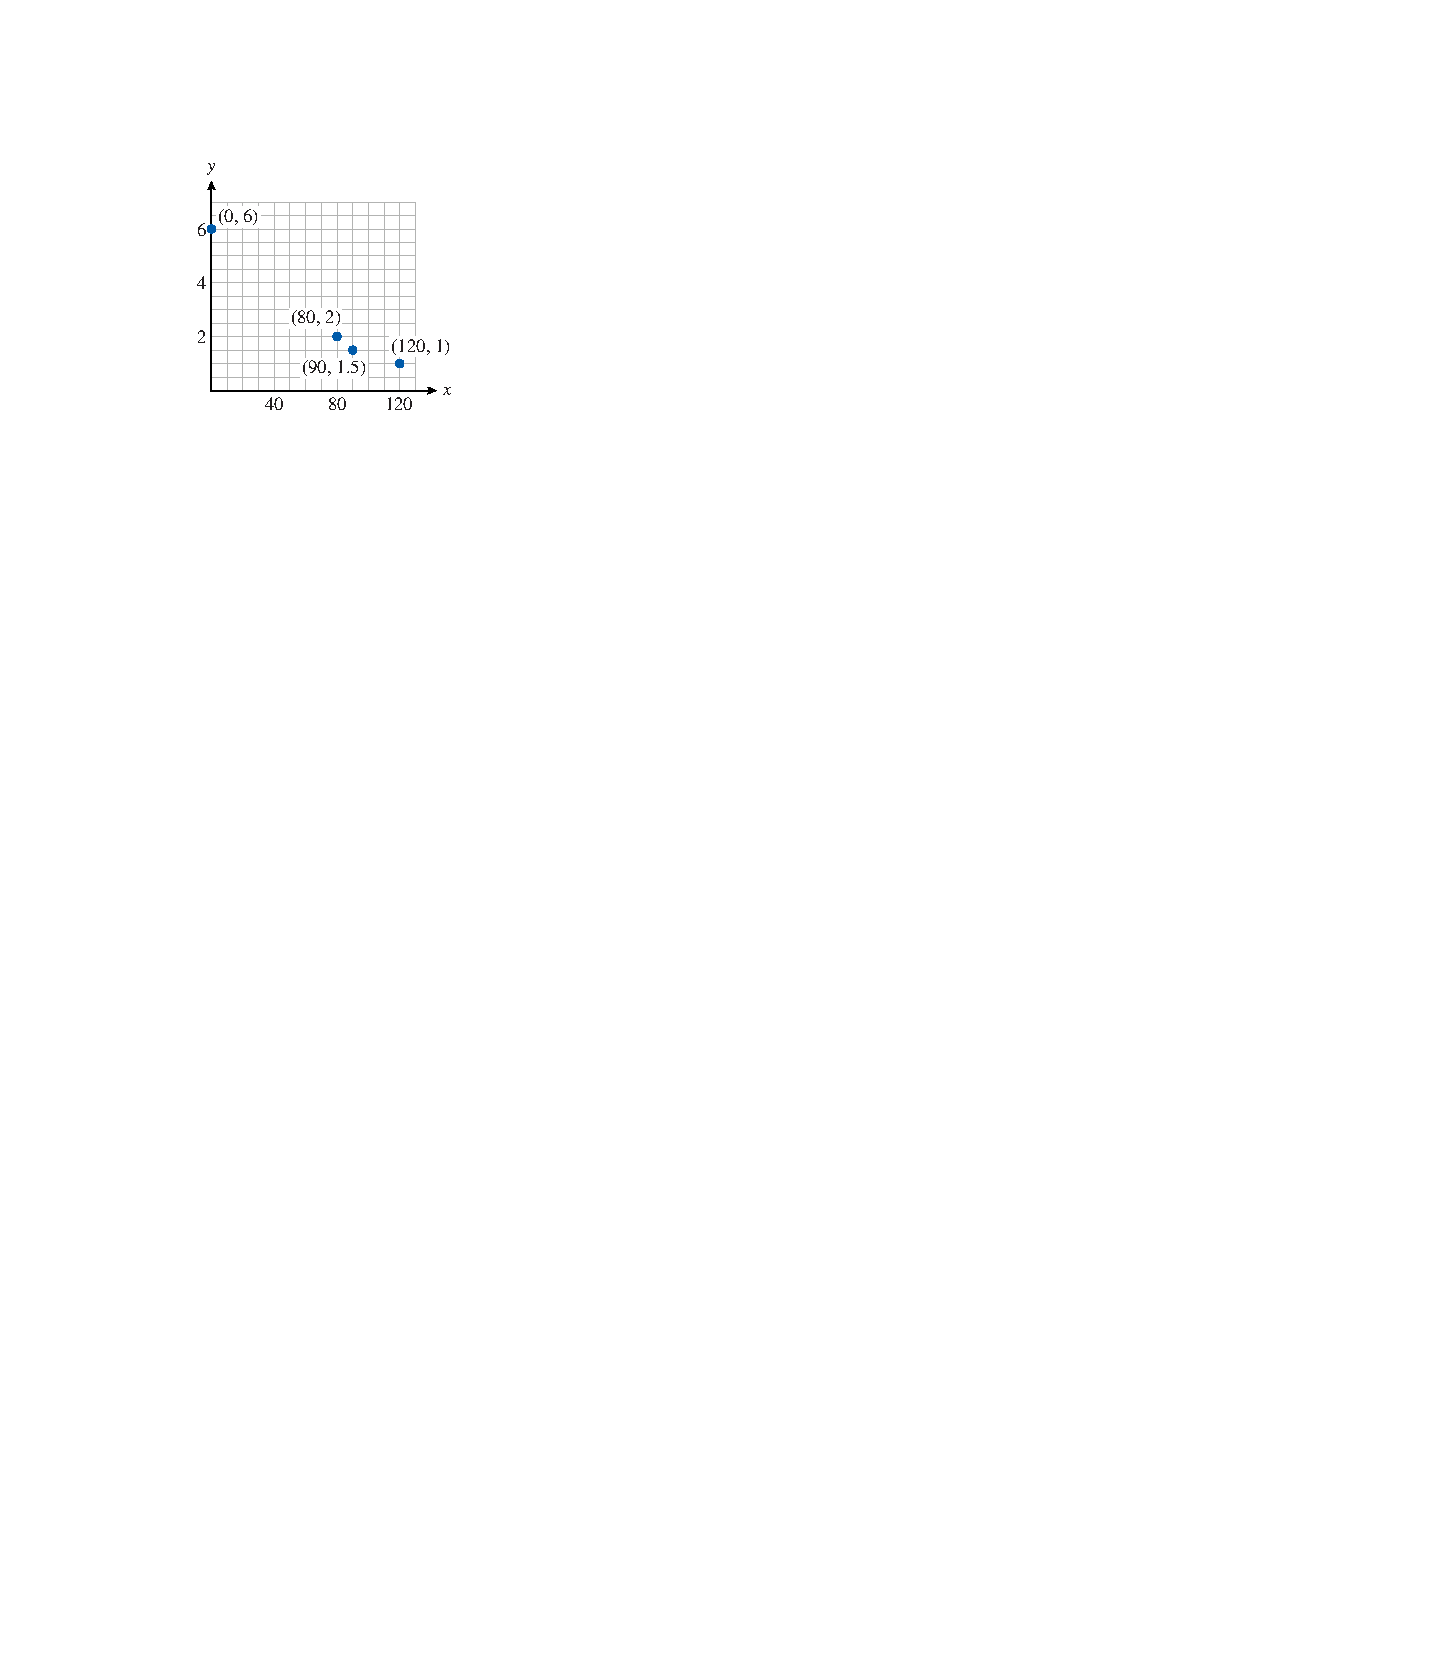
\includegraphics[width=\linewidth]{images/fig-ans-1-1-9}
\end{sbspanel}%
\end{sidebyside}%
\end{divisionsolutionegcol}%
\begin{divisionsolutionegcol}{1.1.7.10}{}{g:exercise:idm93552238656}%
\begin{sidebyside}{1}{0}{0}{0}%
\begin{sbspanel}{1}%
{\centering%
{\tabularfont%
\begin{tabular}{AlAcAcAcAcA}\hrulethick
\(x\)&\(300\)&\(500\)&\(800\)&\(1100\)\tabularnewline\hrulethin
\(y\)&\(1.2\)&\(1.3\)&\(1.5\)&\(1.9\)\tabularnewline\hrulethin
\end{tabular}
}%
\par}
\end{sbspanel}%
\end{sidebyside}%
\end{divisionsolutionegcol}%
\begin{divisionsolutionegcol}{1.1.7.11}{}{g:exercise:idm93552226320}%
\begin{sidebyside}{1}{0}{0}{0}%
\begin{sbspanel}{1}%
{\centering%
{\tabularfont%
\begin{tabular}{AlAcAcAcAcA}\hrulethick
\(x\)&\(0.01\)&\(0.03\)&\(0.06\)&\(0.07\)\tabularnewline\hrulethin
\(y\)&\(-0.2\)&\(-1\)&\(-1.1\)&\(-2\)\tabularnewline\hrulethin
\end{tabular}
}%
\par}
\end{sbspanel}%
\end{sidebyside}%
\par\smallskip%
\noindent\textbf{\blocktitlefont Answer}.\quad{}\begin{sidebyside}{1}{0.2}{0.2}{0}%
\begin{sbspanel}{0.6}%
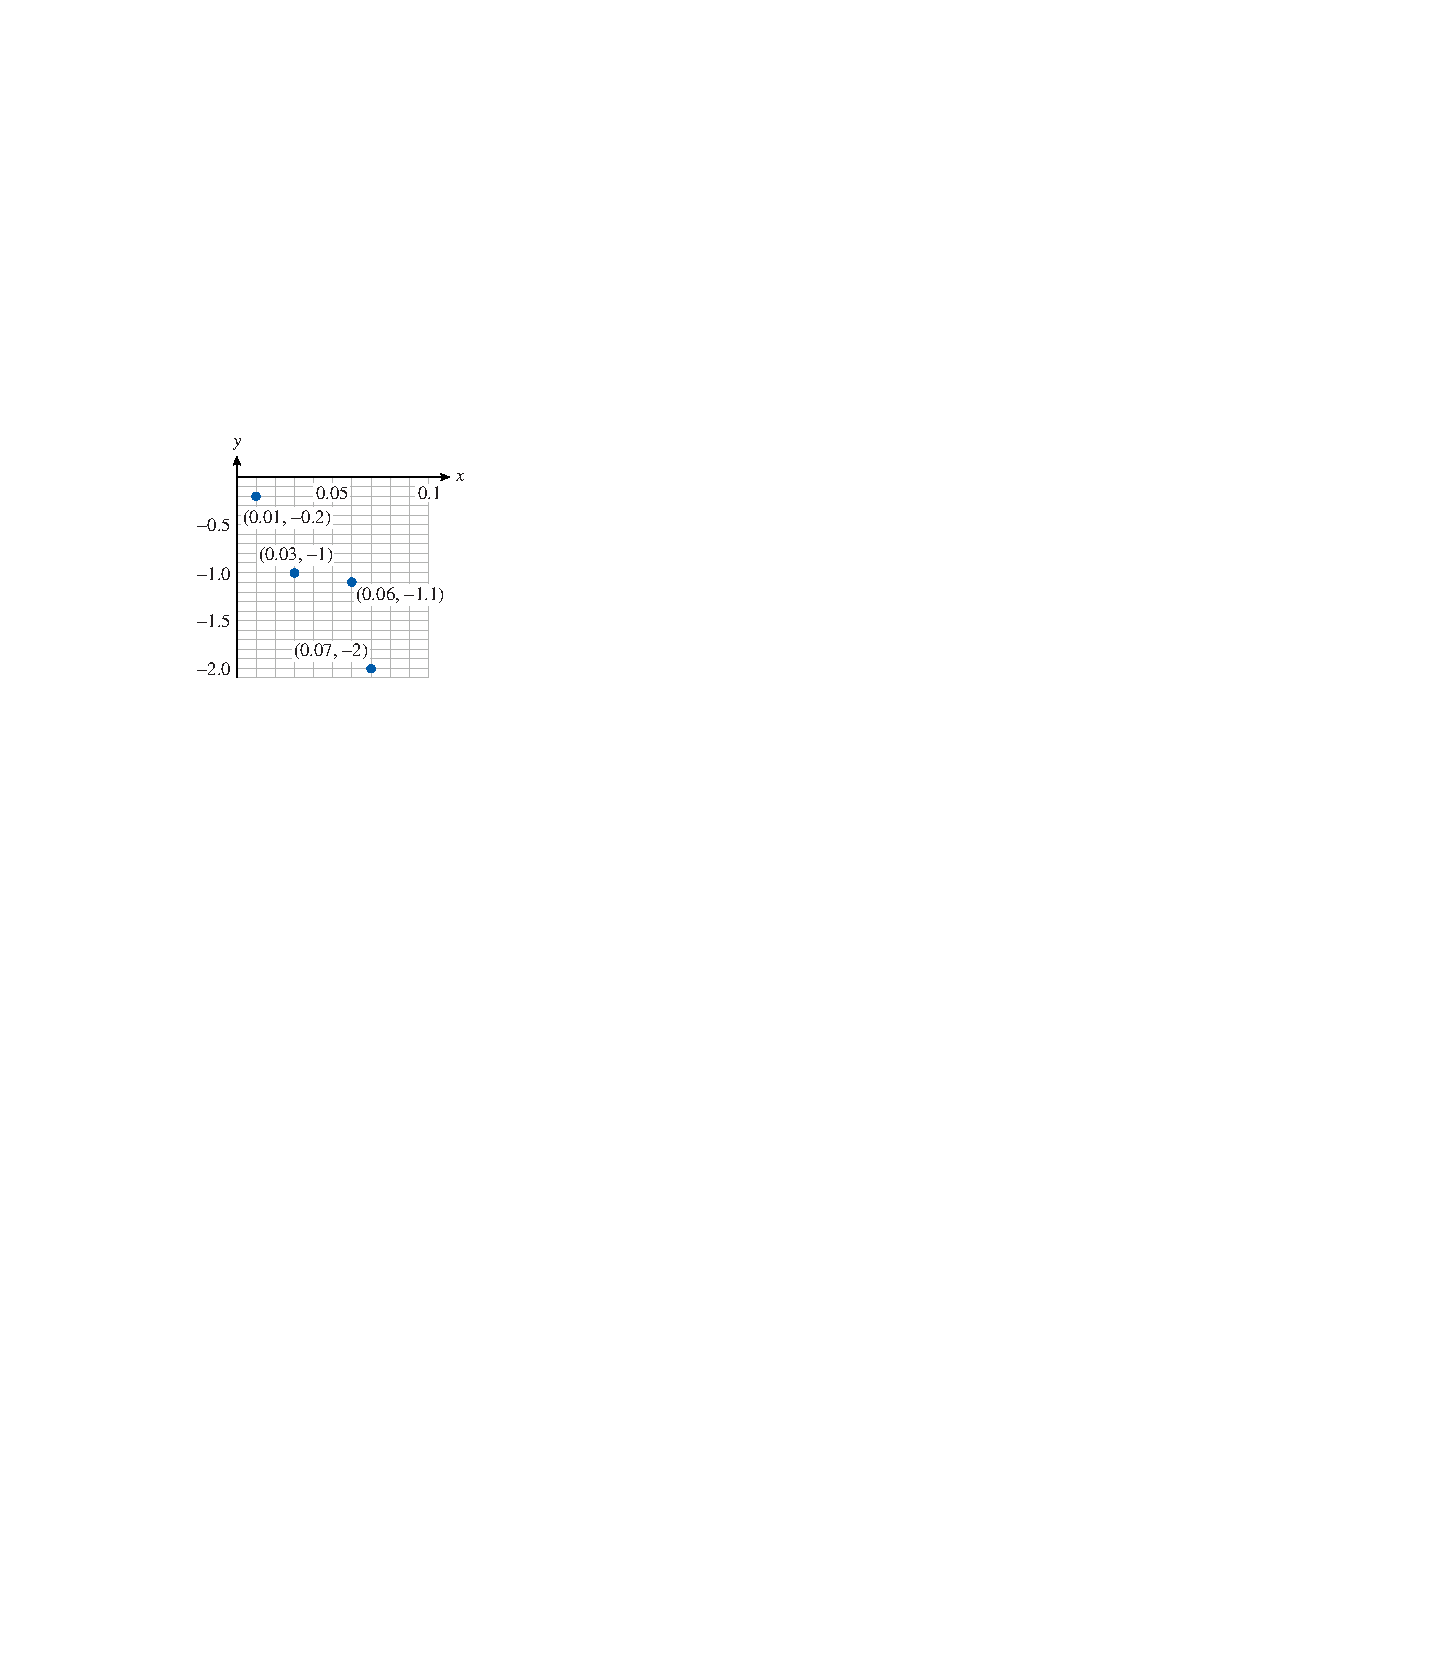
\includegraphics[width=\linewidth]{images/fig-ans-1-1-11}
\end{sbspanel}%
\end{sidebyside}%
\end{divisionsolutionegcol}%
\begin{divisionsolutionegcol}{1.1.7.12}{}{g:exercise:idm93552212528}%
\begin{sidebyside}{1}{0}{0}{0}%
\begin{sbspanel}{1}%
{\centering%
{\tabularfont%
\begin{tabular}{AlAcAcAcAcA}\hrulethick
\(x\)&\(0.003\)&\(0.005\)&\(0.008\)&\(0.011\)\tabularnewline\hrulethin
\(y\)&\(6\)&\(2\)&\(1.5\)&\(1\)\tabularnewline\hrulethin
\end{tabular}
}%
\par}
\end{sbspanel}%
\end{sidebyside}%
\end{divisionsolutionegcol}%
\end{exercisegroupcol}
\par\medskip\noindent
For Problems 13-18,%
\begin{enumerate}[label=(\alph*)]
\item{}Find the intercepts of the graph.%
\item{}Graph the equation by the intercept method.%
\end{enumerate}
%
\begin{exercisegroupcol}{2}
\begin{divisionsolutionegcol}{1.1.7.13}{}{g:exercise:idm93552197664}%
\(x + 2y = 8\)%
\par\smallskip%
\noindent\textbf{\blocktitlefont Answer}.\quad{}%
\begin{enumerate}[label=\alph*]
\item{}\((8, 0), (0, 4)\)%
\item{}\begin{sidebyside}{1}{0}{0}{0}%
\begin{sbspanel}{1}%
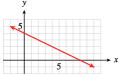
\includegraphics[width=\linewidth]{images/fig-ans-1-1-13}
\end{sbspanel}%
\end{sidebyside}%
%
\end{enumerate}
%
\end{divisionsolutionegcol}%
\begin{divisionsolutionegcol}{1.1.7.14}{}{g:exercise:idm93552193424}%
\(2x - y = 6\)%
\end{divisionsolutionegcol}%
\begin{divisionsolutionegcol}{1.1.7.15}{}{g:exercise:idm93552192384}%
\(3x - 4y =12\)%
\par\smallskip%
\noindent\textbf{\blocktitlefont Answer}.\quad{}%
\begin{enumerate}[label=\alph*]
\item{}\((4, 0), (0, -3)\)%
\item{}\begin{sidebyside}{1}{0.1}{0.1}{0}%
\begin{sbspanel}{0.8}%
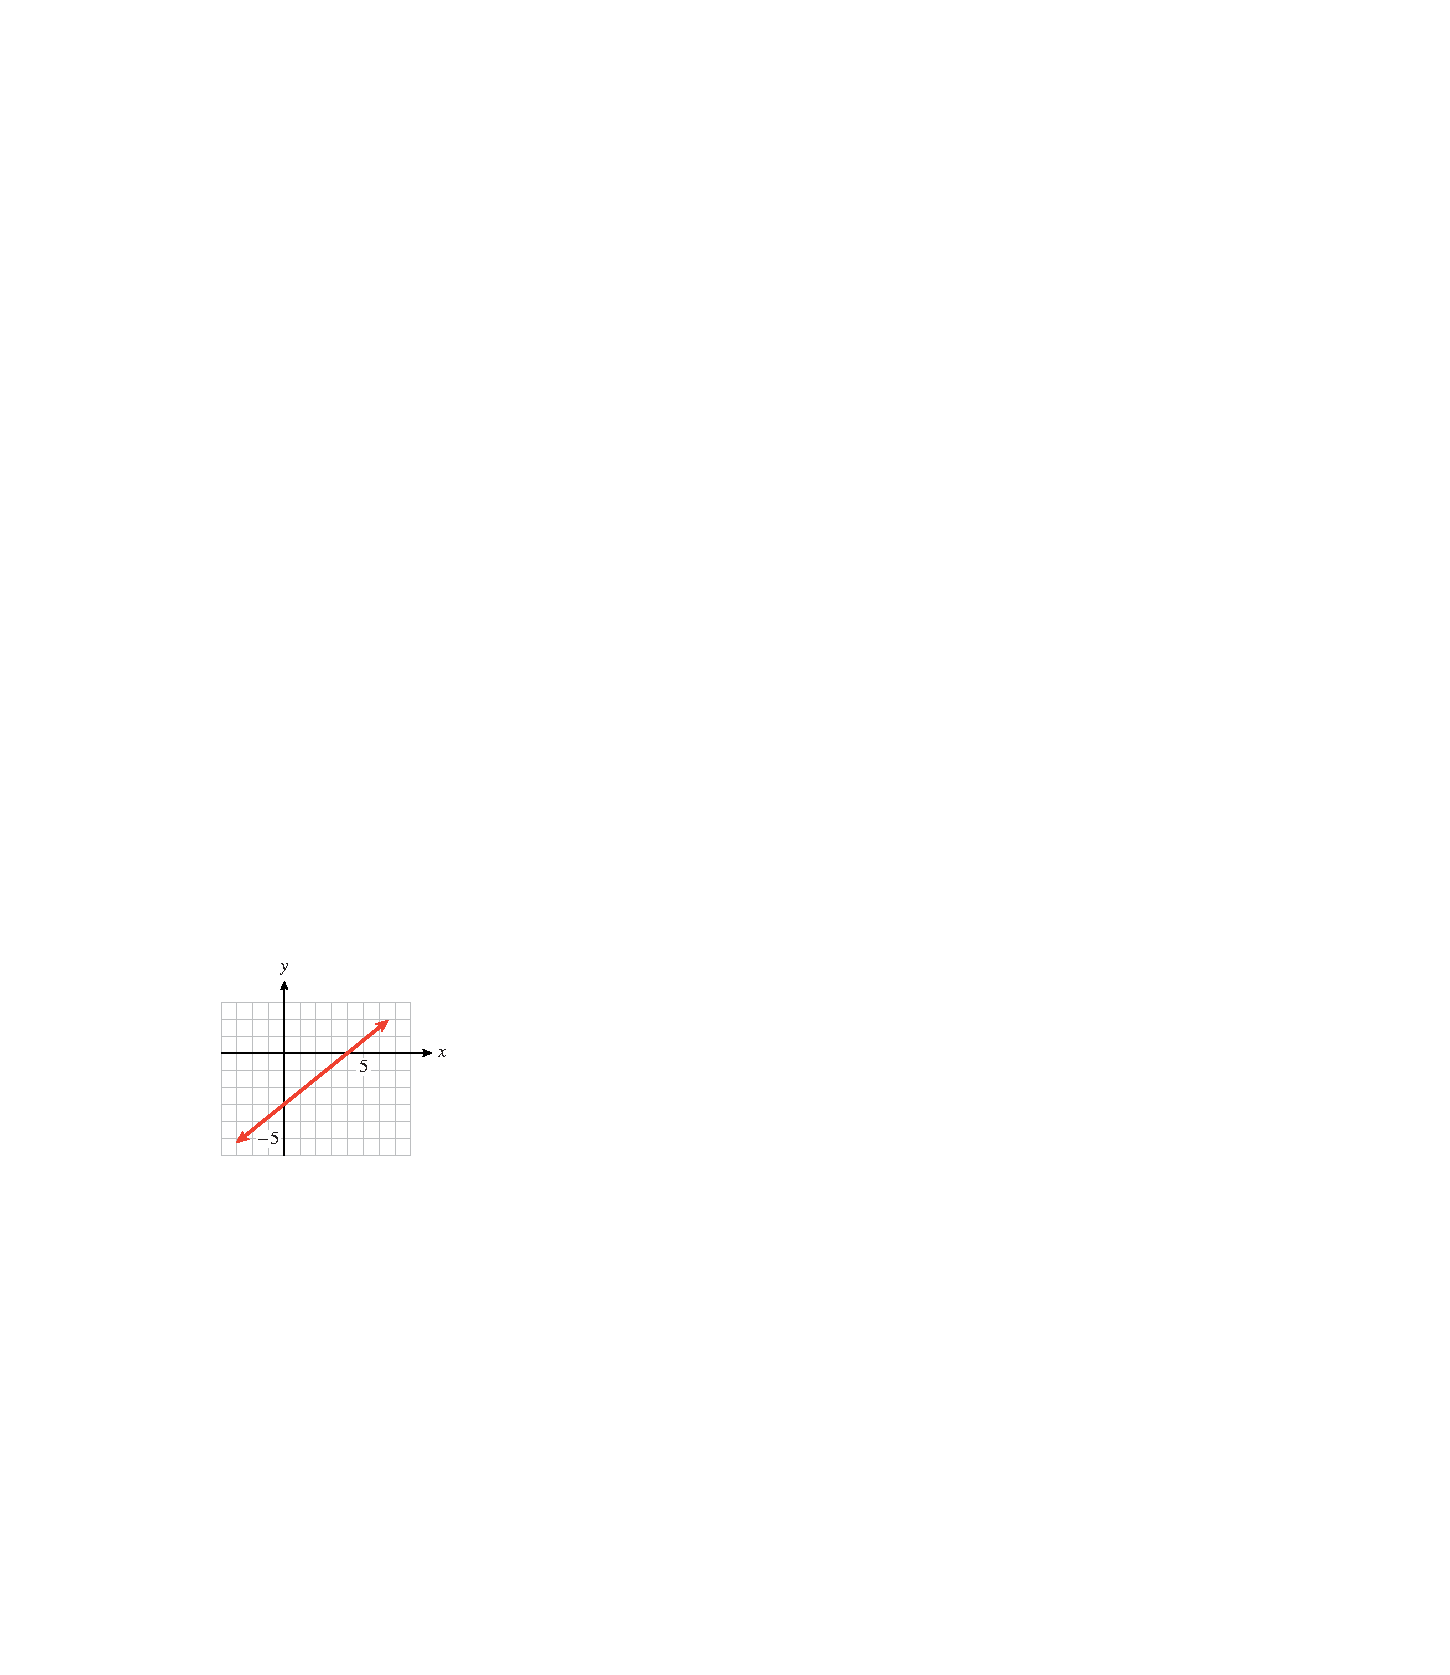
\includegraphics[width=\linewidth]{images/fig-ans-1-1-15}
\end{sbspanel}%
\end{sidebyside}%
%
\end{enumerate}
%
\end{divisionsolutionegcol}%
\begin{divisionsolutionegcol}{1.1.7.16}{}{g:exercise:idm93552188144}%
\(2x + 6y = 6\)%
\end{divisionsolutionegcol}%
\begin{divisionsolutionegcol}{1.1.7.17}{}{g:exercise:idm93552187104}%
\(\displaystyle{\frac{x}{9}- \frac{y}{4}= 1}\)%
\par\smallskip%
\noindent\textbf{\blocktitlefont Answer}.\quad{}%
\begin{enumerate}[label=\alph*]
\item{}\((9, 0), (0, -4)\)%
\item{}\begin{sidebyside}{1}{0}{0}{0}%
\begin{sbspanel}{1}%
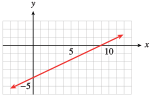
\includegraphics[width=\linewidth]{images/fig-ans-1-1-17}
\end{sbspanel}%
\end{sidebyside}%
%
\end{enumerate}
%
\end{divisionsolutionegcol}%
\begin{divisionsolutionegcol}{1.1.7.18}{}{g:exercise:idm93552182976}%
\(\displaystyle{\frac{x}{5}+ \frac{y}{8}= 1}\)%
\end{divisionsolutionegcol}%
\end{exercisegroupcol}
\par\medskip\noindent
For Problems 19-24,%
\begin{enumerate}[label=(\alph*)]
\item{}Find the intercepts of the graph.%
\item{}Use the intercepts to choose scales for the axes, and then graph the equation by the intercept method.%
\end{enumerate}
%
\begin{exercisegroupcol}{2}
\begin{divisionsolutionegcol}{1.1.7.19}{}{g:exercise:idm93552179312}%
\(20x = 30y - 45,000\)%
\par\smallskip%
\noindent\textbf{\blocktitlefont Answer}.\quad{}%
\begin{enumerate}[label=\alph*]
\item{}\((-2250, 0), (0, 1500)\)%
\item{}\begin{sidebyside}{1}{0.15}{0.15}{0}%
\begin{sbspanel}{0.7}%
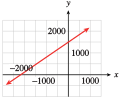
\includegraphics[width=\linewidth]{images/fig-ans-1-1-19}
\end{sbspanel}%
\end{sidebyside}%
%
\end{enumerate}
%
\end{divisionsolutionegcol}%
\begin{divisionsolutionegcol}{1.1.7.20}{}{g:exercise:idm93552175328}%
\(30x = 45y + 60,000\)%
\end{divisionsolutionegcol}%
\begin{divisionsolutionegcol}{1.1.7.21}{}{g:exercise:idm93552174272}%
\(0.4x + 1.2y = 4.8\)%
\par\smallskip%
\noindent\textbf{\blocktitlefont Answer}.\quad{}%
\begin{enumerate}[label=\alph*]
\item{}\((12, 0), (0, 4)\)%
\item{}\begin{sidebyside}{1}{0.075}{0.075}{0}%
\begin{sbspanel}{0.85}%
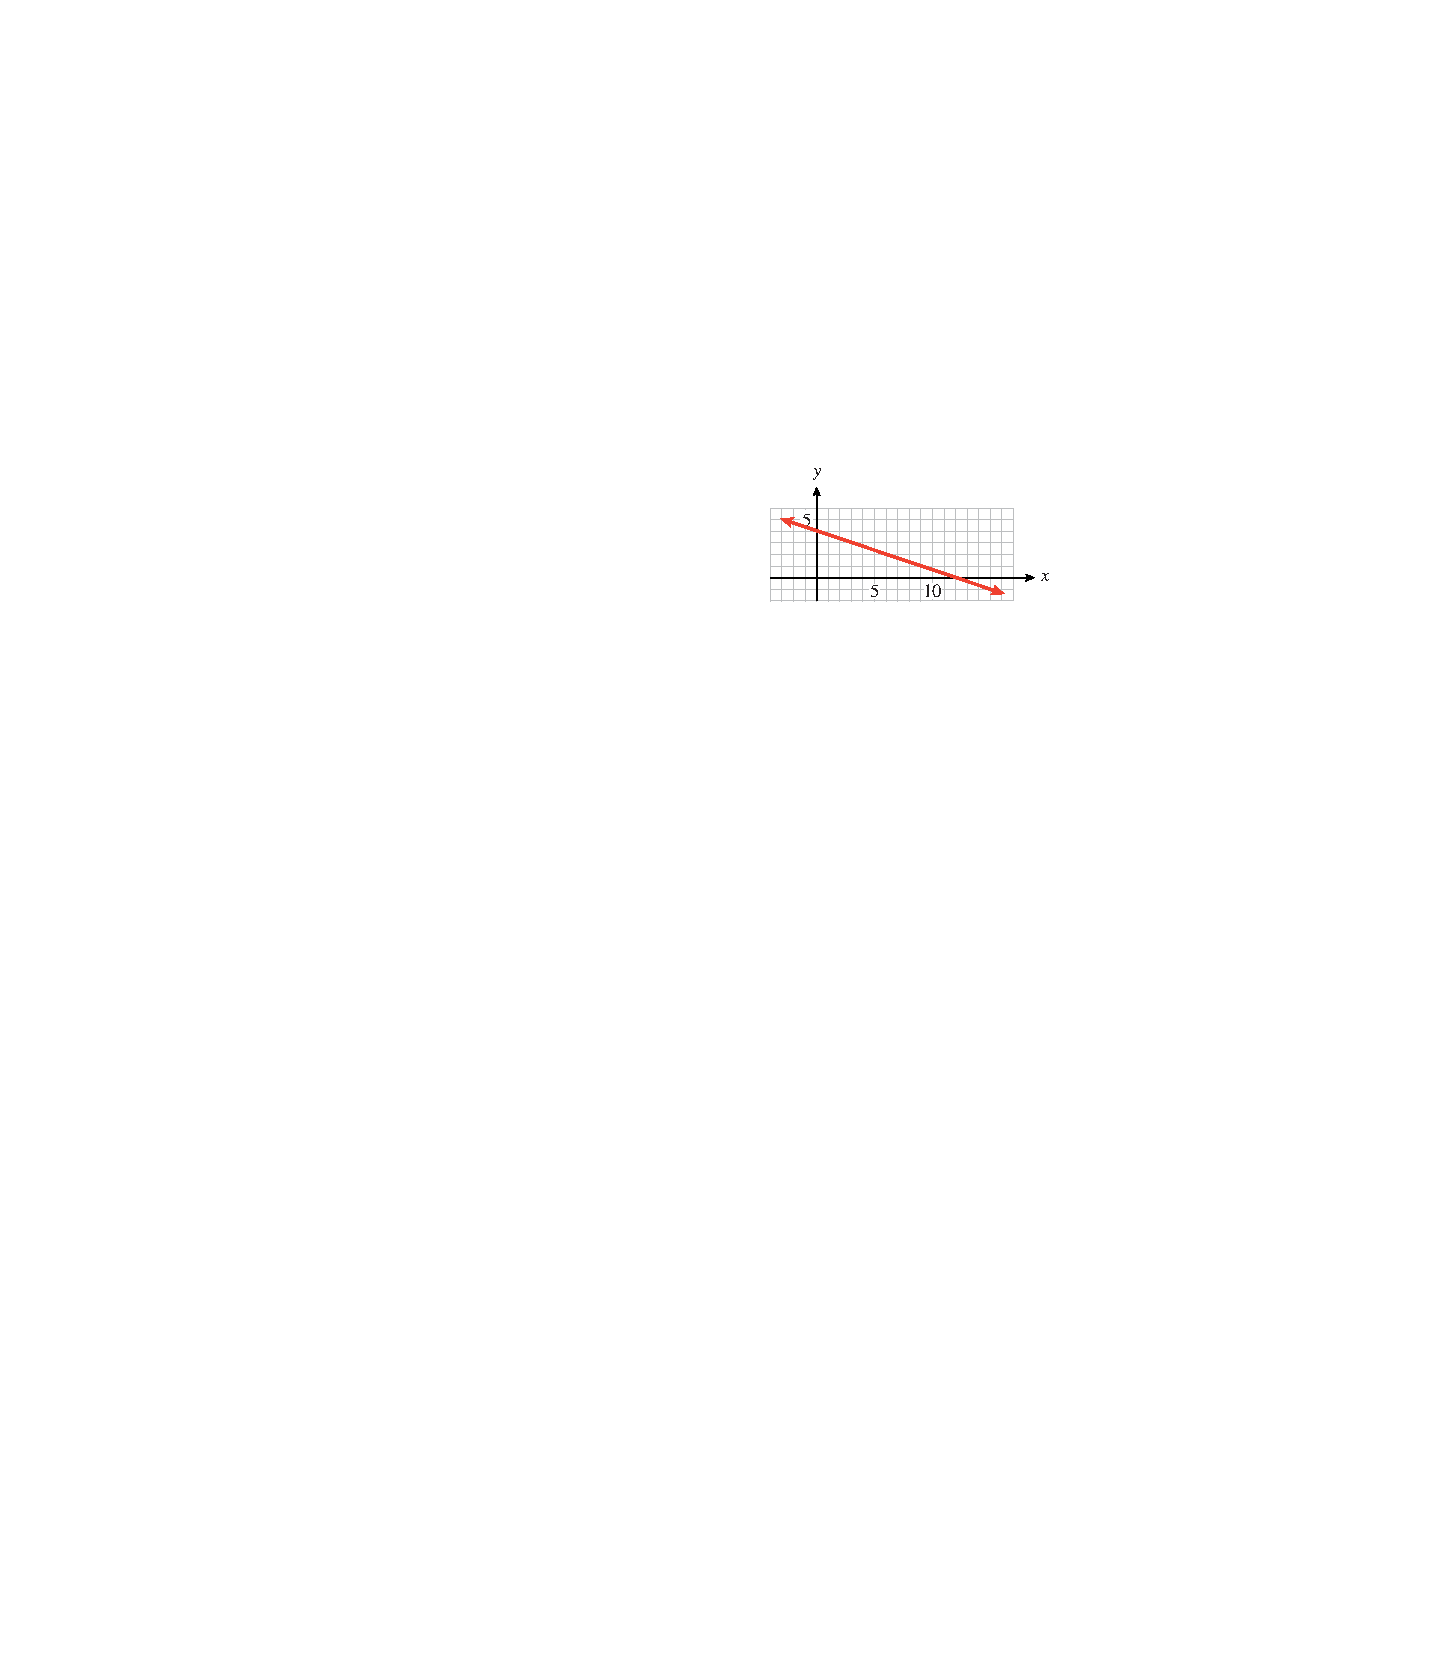
\includegraphics[width=\linewidth]{images/fig-ans-1-1-21}
\end{sbspanel}%
\end{sidebyside}%
%
\end{enumerate}
%
\end{divisionsolutionegcol}%
\begin{divisionsolutionegcol}{1.1.7.22}{}{g:exercise:idm93552170016}%
\(3.2x - 0.8y = 12.8\)%
\end{divisionsolutionegcol}%
\begin{divisionsolutionegcol}{1.1.7.23}{}{g:exercise:idm93552168960}%
\(\displaystyle{\frac{2x}{3}+ \frac{3y}{11}= 1}\)%
\par\smallskip%
\noindent\textbf{\blocktitlefont Answer}.\quad{}%
\begin{enumerate}[label=\alph*]
\item{}\(\left(\dfrac{3}{2} , 0\right), \left(0, \dfrac{11}{3} \right)\)%
\item{}\begin{sidebyside}{1}{0.15}{0.15}{0}%
\begin{sbspanel}{0.7}%
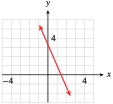
\includegraphics[width=\linewidth]{images/fig-ans-1-1-23}
\end{sbspanel}%
\end{sidebyside}%
%
\end{enumerate}
%
\end{divisionsolutionegcol}%
\begin{divisionsolutionegcol}{1.1.7.24}{}{g:exercise:idm93552164784}%
\(\displaystyle{\frac{8x}{7}- \frac{2y}{7}= 1}\)%
\end{divisionsolutionegcol}%
\end{exercisegroupcol}
\par\medskip\noindent
\begin{divisionsolution}{1.1.7.25}{}{g:exercise:idm93552163568}%
The owner of a gas station has \textdollar{}\(19,200\) to spend on unleaded gas this month. Regular unleaded costs him \textdollar{}\(2.40\) per gallon, and premium unleaded costs \textdollar{}\(3.20\) per gallon.%
%
\begin{enumerate}[label=\alph*]
\item{}How much do \(x\) gallons of regular cost? How much do \(y\) gallons of premium cost?%
\item{}Write an equation in general form that relates the amount of regular unleaded gasoline, \(x\), the owner can buy and the amount of premium unleaded, \(y\).%
\item{}Find the intercepts and sketch the graph.%
\item{}What do the intercepts tell us about the amount of gasoline the owner can purchase?%
\end{enumerate}
\par\smallskip%
\noindent\textbf{\blocktitlefont Answer}.\quad{}%
\begin{enumerate}[label=\alph*]
\item{}\textdollar{}\(2.40x,\) \textdollar{}\(3.20y\)%
\item{}\(2.40x + 3.20y = 19,200\)%
\item{}\begin{sidebyside}{1}{0}{0.6}{0}%
\begin{sbspanel}{0.4}%
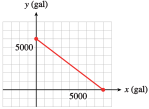
\includegraphics[width=\linewidth]{images/fig-ans-1-1-25}
\end{sbspanel}%
\end{sidebyside}%
%
\item{}The \(y\)-intercept, \(6000\) gallons, is the amount of premium that the gas station owner can buy if he buys no regular. The \(x\)-intercept, \(8000\) gallons, is the amount of regular he can buy if he buys no premium.%
\end{enumerate}
%
\end{divisionsolution}%
\begin{divisionsolution}{1.1.7.26}{}{g:exercise:idm93552149488}%
Five pounds of body fat is equivalent to \(16,000\) calories. Carol can burn \(600\) calories per hour bicycling and \(400\) calories per hour swimming.%
%
\begin{enumerate}[label=\alph*]
\item{}How many calories will Carol burn in \(x\) hours of cycling? How many calories will she burn in \(y\) hours of swimming?%
\item{}Write an equation in general form that relates the number of hours, \(x\), of cycling and the number of hours, \(y\), of swimming Carol needs to perform in order to lose \(5\) pounds.%
\item{}Find the intercepts and sketch the graph.%
\item{}What do the intercepts tell us about Carol's exercise program?%
\end{enumerate}
\end{divisionsolution}%
\begin{divisionsolution}{1.1.7.27}{}{g:exercise:idm93552141936}%
Delbert must increase his daily potassium intake by \(1800\) mg. He decides to eat a combination of figs and bananas, which are both low in sodium. There are \(9\) mg potassium per gram of fig, and \(4\) mg potassium per gram of banana.%
%
\begin{enumerate}[label=\alph*]
\item{}How much potassium is in \(x\) grams of fig? How much potassium is in \(y\) grams of banana?%
\item{}Write an equation in general form that relates the number of grams, \(x\), of fig and the number of grams, \(y\), of banana Delbert needs to get \(1800\) mg of potassium.%
\item{}Find the intercepts and sketch the graph.%
\item{}What do the intercepts tell us about Delbert's diet?%
\end{enumerate}
\par\smallskip%
\noindent\textbf{\blocktitlefont Answer}.\quad{}%
\begin{enumerate}[label=\alph*]
\item{}\(9x\) mg, \(4y\) mg%
\item{}\(9x + 4y = 1800\)%
\item{}\begin{sidebyside}{1}{0}{0.75}{0}%
\begin{sbspanel}{0.25}%
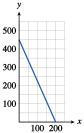
\includegraphics[width=\linewidth]{images/fig-ans-1-1-27}
\end{sbspanel}%
\end{sidebyside}%
%
\item{}The \(x\)-intercept, \(200\) grams, tells how much fig Delbert should eat if he has no bananas, and the \(y\)-intercept, \(450\) grams, tells how much banana he should eat if he has no figs.%
\end{enumerate}
%
\end{divisionsolution}%
\begin{divisionsolution}{1.1.7.28}{}{g:exercise:idm93552127424}%
Leslie plans to invest some money in two CD accounts. The first account pays \(3.6\%\) interest per year, and the second account pays \(2.8\%\) interest per year. Leslie would like to earn \textdollar{}\(500\) per year on her investment.%
%
\begin{enumerate}[label=\alph*]
\item{}If Leslie invests \(x\) dollars in the first account, how much interest will she earn? How much interest will she earn if she invests \(y\) dollars in the second account?%
\item{}Write an equation in general form that relates \(x\) and \(y\) if Leslie earns \(\$500\) interest.%
\item{}Find the intercepts and sketch the graph.%
\item{}What do the intercepts tell us about Leslie's investments?%
\end{enumerate}
\end{divisionsolution}%
\begin{divisionsolution}{1.1.7.29}{}{g:exercise:idm93552119872}%
Find the intercepts of the graph for each equation.%
%
\begin{multicols}{2}
\begin{enumerate}[label=\alph*]
\item{}\(\displaystyle{\frac{x}{3}+\frac{y}{5}=1} \)%
\item{}\(\displaystyle{2x - 4y = 1} \)%
\item{}\(\displaystyle{\frac{2x}{5}-\frac{2y}{3}=1} \)%
\item{}\(\displaystyle{\frac{x}{p}+\frac{y}{q}=1} \)%
\end{enumerate}
\end{multicols}
\(\hphantom{00}\) e.  Why is the equation \(\displaystyle{\frac{x}{a}+\frac{y}{b}=1} \) called the \terminology{intercept form} for a line?%
\par\smallskip%
\noindent\textbf{\blocktitlefont Answer}.\quad{}%
\begin{multicols}{2}
\begin{enumerate}[label=\alph*]
\item{}\((3,0), (0,5) \)%
\item{}\(\left(\dfrac{1}{2},0\right), \left(0,\dfrac{-1}{4}\right) \)%
\item{}\(\left(\dfrac{5}{2},0\right), \left(0,\dfrac{-3}{2}\right) \)%
\item{}\((p,0), (0,q) \)%
\item{}The value of \(a\) is the \(x\)-intercept, and the value of \(b\) is the \(y\)-intercept.%
\end{enumerate}
\end{multicols}
%
\end{divisionsolution}%
\begin{divisionsolution}{1.1.7.30}{}{g:exercise:idm93552107184}%
Write an equation in intercept form (see Problem 29) for the line with the given intercepts. Then write the equation in general form.%
%
\begin{multicols}{2}
\begin{enumerate}[label=\alph*]
\item{}\((6, 0), (0, 2) \)%
\item{}\((-3, 0), (0, 8) \)%
\item{}\(\left(\dfrac{3}{4}, 0\right), \left(0, \dfrac{-1}{4}\right) \)%
\item{}\((v, 0), (0, -w) \)%
\item{}\(\left(\dfrac{1}{H}, 0\right), \left(0, \dfrac{1}{T}\right) \)%
\end{enumerate}
\end{multicols}
\end{divisionsolution}%
\begin{divisionsolution}{1.1.7.31}{}{g:exercise:idm93552101680}%
%
\begin{enumerate}[label=\alph*]
\item{}Find the \(y\)-intercept of the line \(y = mx + b\).%
\item{}Find the \(x\)-intercept of the line \(y = mx + b\).%
\end{enumerate}
%
\par\smallskip%
\noindent\textbf{\blocktitlefont Answer}.\quad{}%
\begin{enumerate}[label=\alph*]
\item{}\((0, b)\)%
\item{}\(\left(\dfrac{-b}{m},0\right)\), if \(m\ne 0\)%
\end{enumerate}
%
\end{divisionsolution}%
\begin{divisionsolution}{1.1.7.32}{}{g:exercise:idm93552094720}%
%
\begin{enumerate}[label=\alph*]
\item{}Find the \(y\)-intercept of the line \(Ax + By = C\).%
\item{}Find the \(x\)-intercept of the line \(Ax + By = C\).%
\end{enumerate}
%
\end{divisionsolution}%
Write an equation in general form for each line.%
\begin{exercisegroupcol}{2}
\begin{divisionsolutionegcol}{1.1.7.33}{}{g:exercise:idm93552089664}%
\begin{sidebyside}{1}{0.1}{0.1}{0}%
\begin{sbspanel}{0.8}%
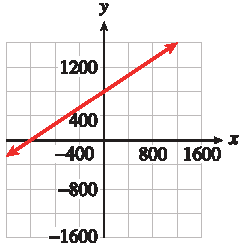
\includegraphics[width=\linewidth]{images/fig-ex-1-1-33}
\end{sbspanel}%
\end{sidebyside}%
\par\smallskip%
\noindent\textbf{\blocktitlefont Answer}.\quad{}\(-2x + 3y = 2400\)%
\end{divisionsolutionegcol}%
\begin{divisionsolutionegcol}{1.1.7.34}{}{g:exercise:idm93552087184}%
\begin{sidebyside}{1}{0.1}{0.1}{0}%
\begin{sbspanel}{0.8}%
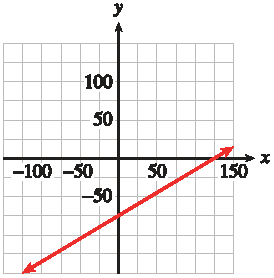
\includegraphics[width=\linewidth]{images/fig-ex-1-1-34}
\end{sbspanel}%
\end{sidebyside}%
\end{divisionsolutionegcol}%
\begin{divisionsolutionegcol}{1.1.7.35}{}{g:exercise:idm93552085376}%
\begin{sidebyside}{1}{0.1}{0.1}{0}%
\begin{sbspanel}{0.8}%
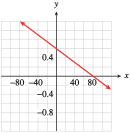
\includegraphics[width=\linewidth]{images/fig-ex-1-1-35}
\end{sbspanel}%
\end{sidebyside}%
\par\smallskip%
\noindent\textbf{\blocktitlefont Answer}.\quad{}\(3x + 400y = 240\)%
\end{divisionsolutionegcol}%
\begin{divisionsolutionegcol}{1.1.7.36}{}{g:exercise:idm93552082896}%
\begin{sidebyside}{1}{0.1}{0.1}{0}%
\begin{sbspanel}{0.8}%
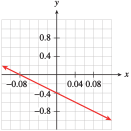
\includegraphics[width=\linewidth]{images/fig-ex-1-1-36}
\end{sbspanel}%
\end{sidebyside}%
\end{divisionsolutionegcol}%
\end{exercisegroupcol}
\par\medskip\noindent
For Problems 37\textendash{}44,%
\begin{enumerate}[label=\alph*]
\item{}Solve each equation for \(y\) in terms of \(x\). (See the Algebra Skills Refresher Section~A.2 to review this skill.)%
\item{}Graph the equation on your calculator in the specified window.%
\item{}Make a pencil and paper sketch of the graph. Label the scales on your axes, and the coordinates of the intercepts.%
\end{enumerate}
%
\begin{exercisegroupcol}{2}
\begin{divisionsolutionegcol}{1.1.7.37}{}{g:exercise:idm93552075776}%
\(2+y=6\)%
\begin{align*}
{\text{Xmin}} \amp = -10 \amp\amp {\text{Ymin}} = -10\\
{\text{Xmax}} \amp = 10 \amp\amp {\text{Ymax}} = 10\\
{\text{Xscl}} \amp = 1 \amp\amp {\text{Yscl}} = 1
\end{align*}
%
\par\smallskip%
\noindent\textbf{\blocktitlefont Answer}.\quad{}%
\begin{enumerate}[label=\alph*]
\item{}\(y = 6 - 2x\)%
\item{}\begin{sidebyside}{1}{0}{0.3}{0}%
\begin{sbspanel}{0.7}%
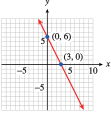
\includegraphics[width=\linewidth]{images/fig-ans-1-1-37}
\end{sbspanel}%
\end{sidebyside}%
%
\end{enumerate}
%
\end{divisionsolutionegcol}%
\begin{divisionsolutionegcol}{1.1.7.38}{}{g:exercise:idm93552069648}%
\(8 - y + 3x = 0\)%
\begin{align*}
{\text{Xmin}} \amp = -10 \amp\amp {\text{Ymin}} = -10\\
{\text{Xmax}} \amp = 10 \amp\amp {\text{Ymax}} = 10\\
{\text{Xscl}} \amp = 1 \amp\amp {\text{Yscl}} = 1
\end{align*}
%
\end{divisionsolutionegcol}%
\begin{divisionsolutionegcol}{1.1.7.39}{}{g:exercise:idm93552066672}%
\(3x - 4y = 1200\)%
\begin{align*}
{\text{Xmin}} \amp = -1000 \amp\amp {\text{Ymin}} = -1000\\
{\text{Xmax}} \amp = 1000 \amp\amp {\text{Ymax}} = 1000\\
{\text{Xscl}} \amp = 100 \amp\amp {\text{Yscl}} = 100
\end{align*}
%
\par\smallskip%
\noindent\textbf{\blocktitlefont Answer}.\quad{}%
\begin{enumerate}[label=\alph*]
\item{}\(y = \dfrac{3}{4}x-300\)%
\item{}\begin{sidebyside}{1}{0}{0.3}{0}%
\begin{sbspanel}{0.7}%
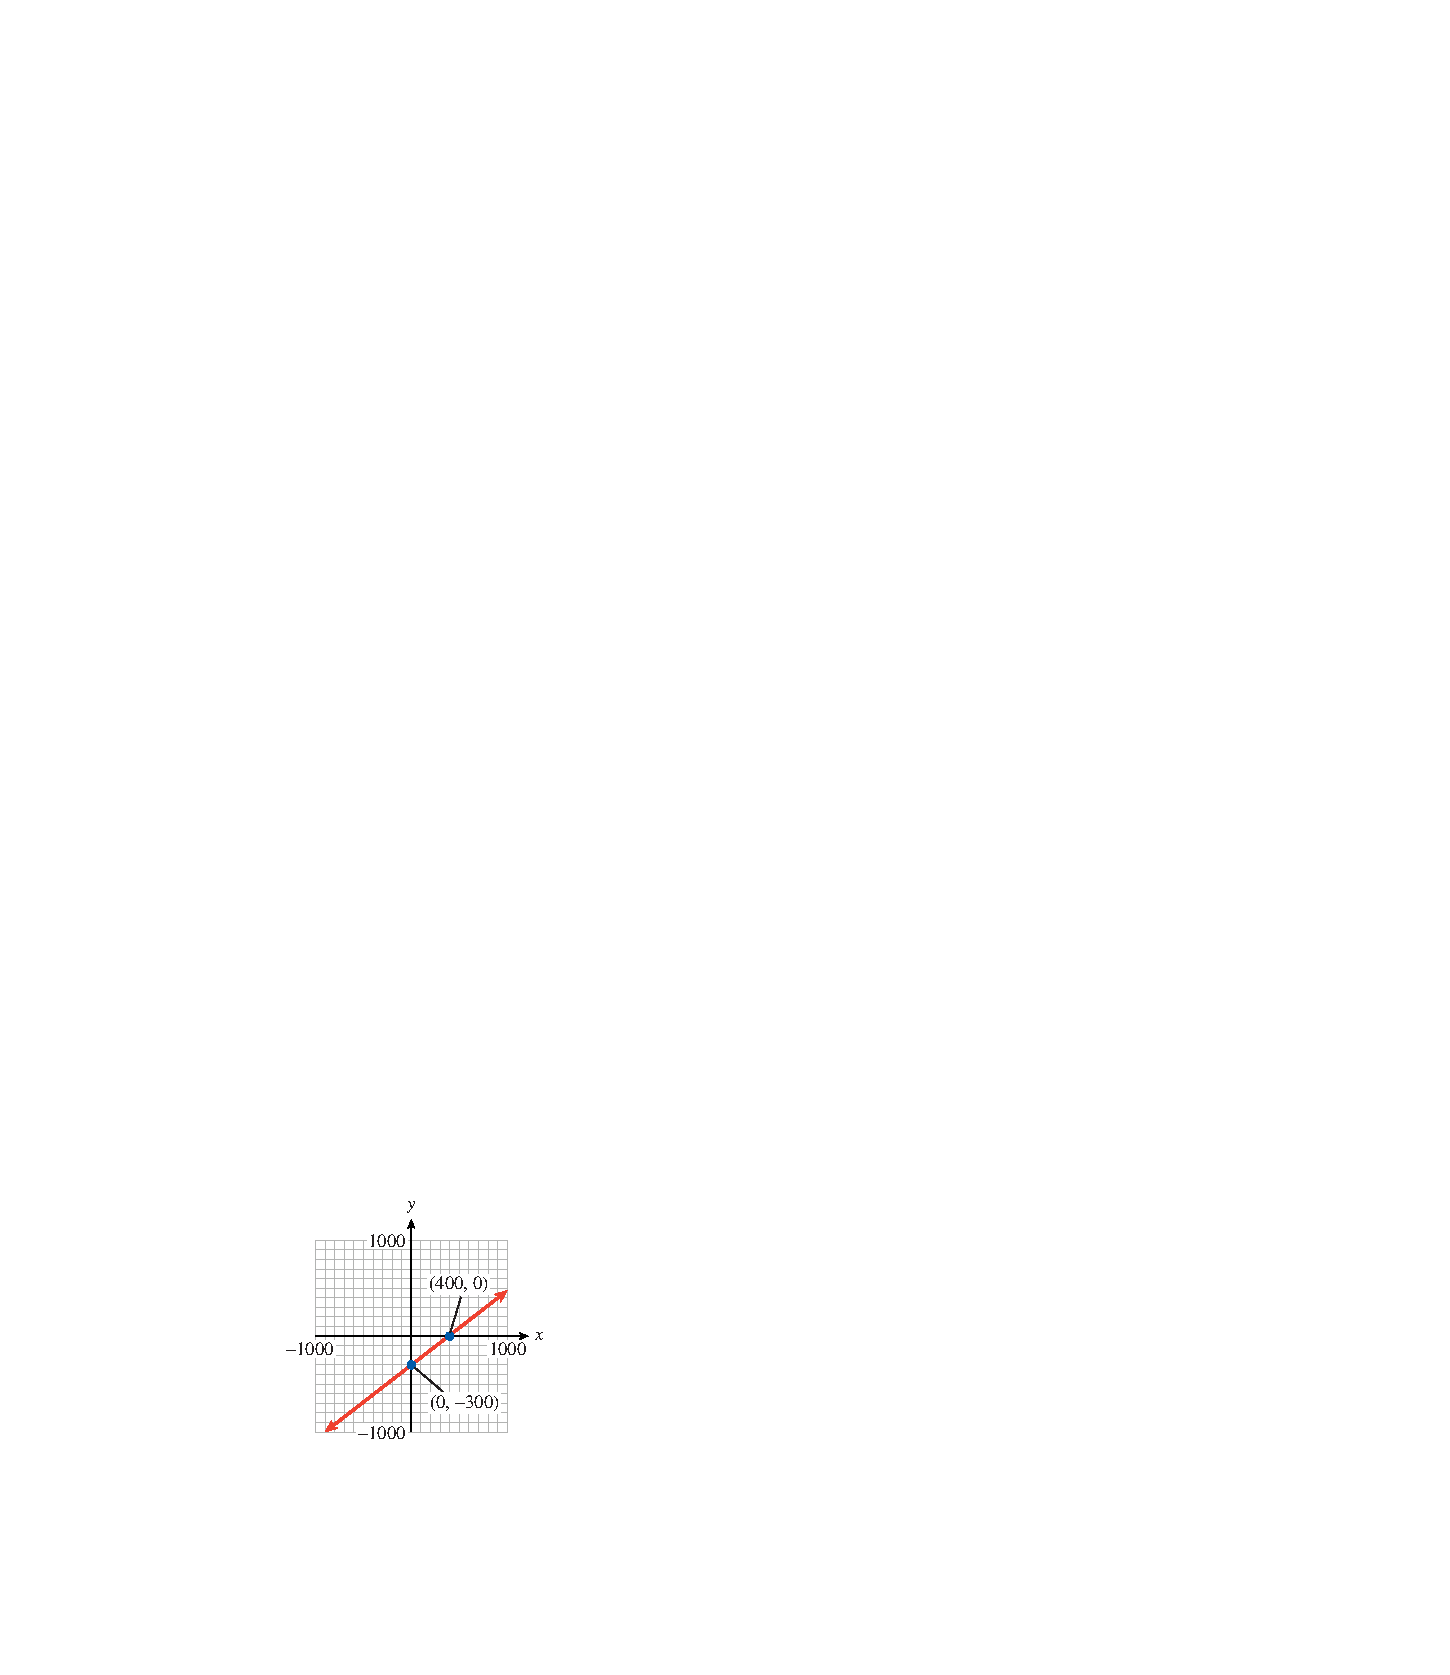
\includegraphics[width=\linewidth]{images/fig-ans-1-1-39}
\end{sbspanel}%
\end{sidebyside}%
%
\end{enumerate}
%
\end{divisionsolutionegcol}%
\begin{divisionsolutionegcol}{1.1.7.40}{}{g:exercise:idm93552060496}%
\(x + 2y = 500\)%
\begin{align*}
{\text{Xmin}} \amp = -1000 \amp\amp {\text{Ymin}} = -1000\\
{\text{Xmax}} \amp = 1000 \amp\amp {\text{Ymax}} = 1000\\
{\text{Xscl}} \amp = 100 \amp\amp {\text{Yscl}} = 100
\end{align*}
%
\end{divisionsolutionegcol}%
\begin{divisionsolutionegcol}{1.1.7.41}{}{g:exercise:idm93552057488}%
\(0.2x + 5y = 0.1\)%
\begin{align*}
{\text{Xmin}} \amp = -1 \amp\amp {\text{Ymin}} = -0.1\\
{\text{Xmax}} \amp = 1 \amp\amp {\text{Ymax}} = 0.1\\
{\text{Xscl}} \amp = 0.1 \amp\amp {\text{Yscl}} = 0.01
\end{align*}
%
\par\smallskip%
\noindent\textbf{\blocktitlefont Answer}.\quad{}%
\begin{enumerate}[label=\alph*]
\item{}\(y = 0.02 - 0.04x\)%
\item{}\begin{sidebyside}{1}{0}{0.3}{0}%
\begin{sbspanel}{0.7}%
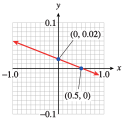
\includegraphics[width=\linewidth]{images/fig-ans-1-1-41}
\end{sbspanel}%
\end{sidebyside}%
%
\end{enumerate}
%
\end{divisionsolutionegcol}%
\begin{divisionsolutionegcol}{1.1.7.42}{}{g:exercise:idm93552051344}%
\(1.2x - 4.2y = 3.6\)%
\begin{align*}
{\text{Xmin}} \amp = -1 \amp\amp {\text{Ymin}} = -1\\
{\text{Xmax}} \amp = 4 \amp\amp {\text{Ymax}} = 1\\
{\text{Xscl}} \amp = 0.2 \amp\amp {\text{Yscl}} = 0.1
\end{align*}
%
\end{divisionsolutionegcol}%
\begin{divisionsolutionegcol}{1.1.7.43}{}{g:exercise:idm93552048352}%
\(70x + 3y = y + 420\)%
\begin{align*}
{\text{Xmin}} \amp = 0 \amp\amp {\text{Ymin}} = 0\\
{\text{Xmax}} \amp = 10 \amp\amp {\text{Ymax}} = 250\\
{\text{Xscl}} \amp = 1 \amp\amp {\text{Yscl}} = 25
\end{align*}
%
\par\smallskip%
\noindent\textbf{\blocktitlefont Answer}.\quad{}%
\begin{enumerate}[label=\alph*]
\item{}\(y = 210 - 35x\)%
\item{}\begin{sidebyside}{1}{0}{0.3}{0}%
\begin{sbspanel}{0.7}%
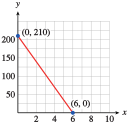
\includegraphics[width=\linewidth]{images/fig-ans-1-1-43}
\end{sbspanel}%
\end{sidebyside}%
%
\end{enumerate}
%
\end{divisionsolutionegcol}%
\begin{divisionsolutionegcol}{1.1.7.44}{}{g:exercise:idm93552042208}%
\(40y - 5x = 780 - 20y\)%
\begin{align*}
{\text{Xmin}} \amp = -200 \amp\amp {\text{Ymin}} = 0\\
{\text{Xmax}} \amp = 0 \amp\amp {\text{Ymax}} = 20\\
{\text{Xscl}} \amp = 20 \amp\amp {\text{Yscl}} = 2
\end{align*}
%
\end{divisionsolutionegcol}%
\end{exercisegroupcol}
\par\medskip\noindent
For Problems 45\textendash{}52,%
\begin{enumerate}[label=\alph*]
\item{}Find the \(x\)- and \(y\)-intercepts.%
\item{}Solve the equation for \(y\).%
\item{}Choose a graphing window in which both intercepts are visible, and graph the equation on your calculator.%
\end{enumerate}
%
\begin{exercisegroupcol}{2}
\begin{divisionsolutionegcol}{1.1.7.45}{}{g:exercise:idm93552034384}%
\(x + 4y = 100\)%
\par\smallskip%
\noindent\textbf{\blocktitlefont Answer}.\quad{}%
\begin{enumerate}[label=\alph*]
\item{}\((100, 0), (0, 25)\)%
\item{}\(y = 25 - \dfrac{1}{4}x\)%
\item{}\begin{sidebyside}{1}{0}{0.3}{0}%
\begin{sbspanel}{0.7}%
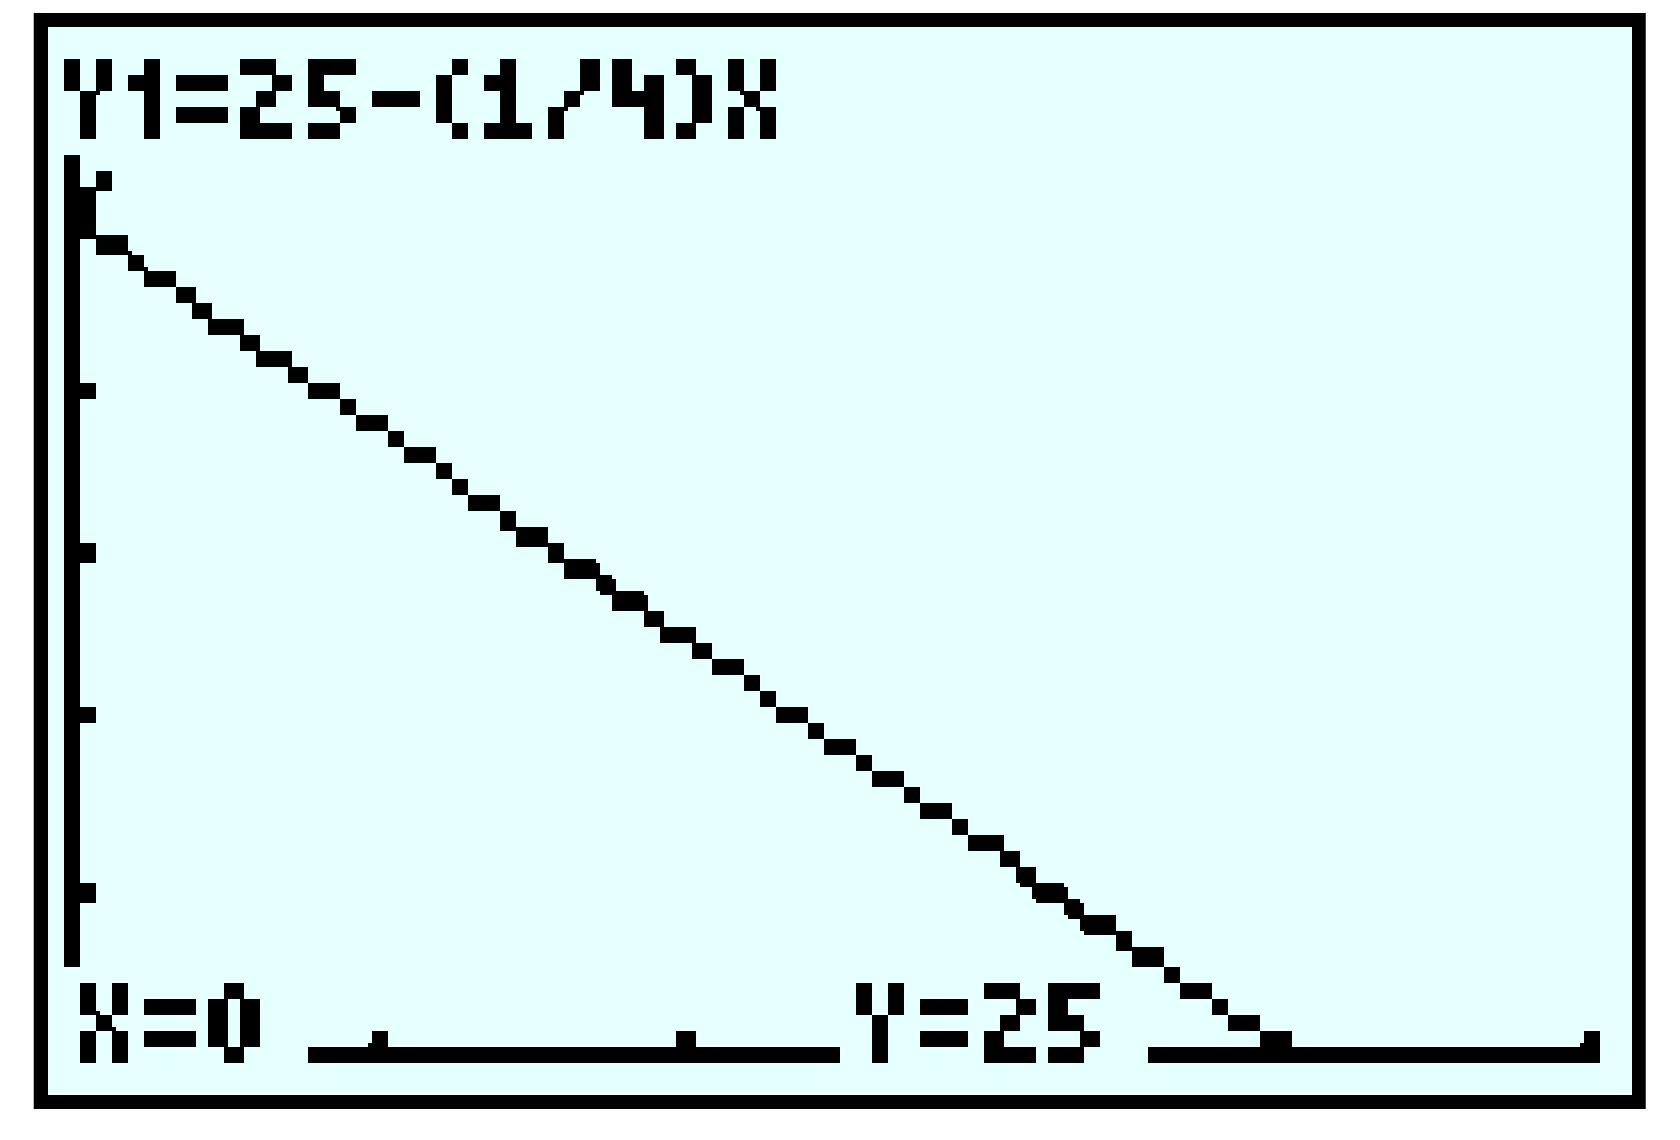
\includegraphics[width=\linewidth]{images/fig-ans-1-1-45.jpg}
\end{sbspanel}%
\end{sidebyside}%
%
\end{enumerate}
%
\end{divisionsolutionegcol}%
\begin{divisionsolutionegcol}{1.1.7.46}{}{g:exercise:idm93552029184}%
\(2x - 3y = -72\)%
\end{divisionsolutionegcol}%
\begin{divisionsolutionegcol}{1.1.7.47}{}{g:exercise:idm93552028000}%
\(25x - 20y = 1\)%
\par\smallskip%
\noindent\textbf{\blocktitlefont Answer}.\quad{}%
\begin{enumerate}[label=\alph*]
\item{}\((0.04, 0), (0, -0.05)\)%
\item{}\(y = 1.25x - 0.05\)%
\item{}\begin{sidebyside}{1}{0}{0.3}{0}%
\begin{sbspanel}{0.7}%
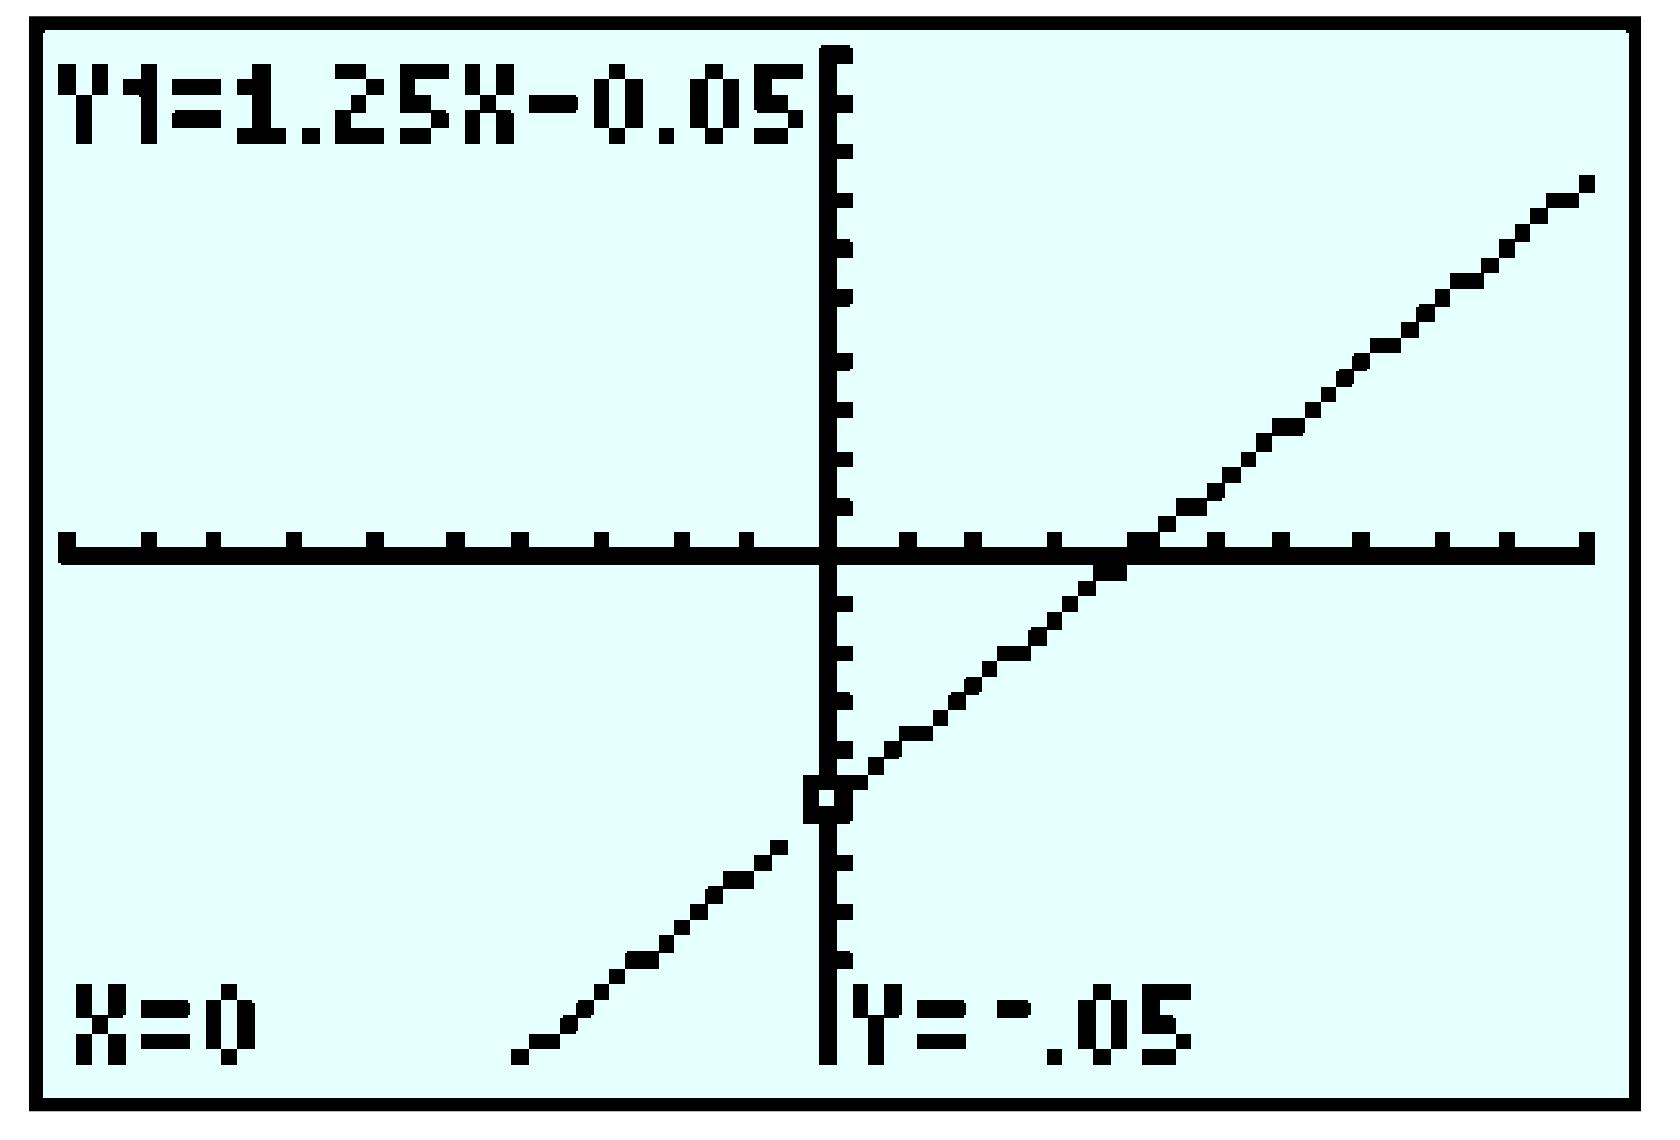
\includegraphics[width=\linewidth]{images/fig-ans-1-1-47.jpg}
\end{sbspanel}%
\end{sidebyside}%
%
\end{enumerate}
%
\end{divisionsolutionegcol}%
\begin{divisionsolutionegcol}{1.1.7.48}{}{g:exercise:idm93552022800}%
\(4x + 75y = 60,000\)%
\end{divisionsolutionegcol}%
\begin{divisionsolutionegcol}{1.1.7.49}{}{g:exercise:idm93552021744}%
\(\dfrac{y}{12} - \dfrac{x}{60}= 1\)%
\par\smallskip%
\noindent\textbf{\blocktitlefont Answer}.\quad{}%
\begin{enumerate}[label=\alph*]
\item{}\((-60, 0), (0, 12)\)%
\item{}\(y = 12 + \dfrac{1}{5}x\)%
\item{}\begin{sidebyside}{1}{0}{0.3}{0}%
\begin{sbspanel}{0.7}%
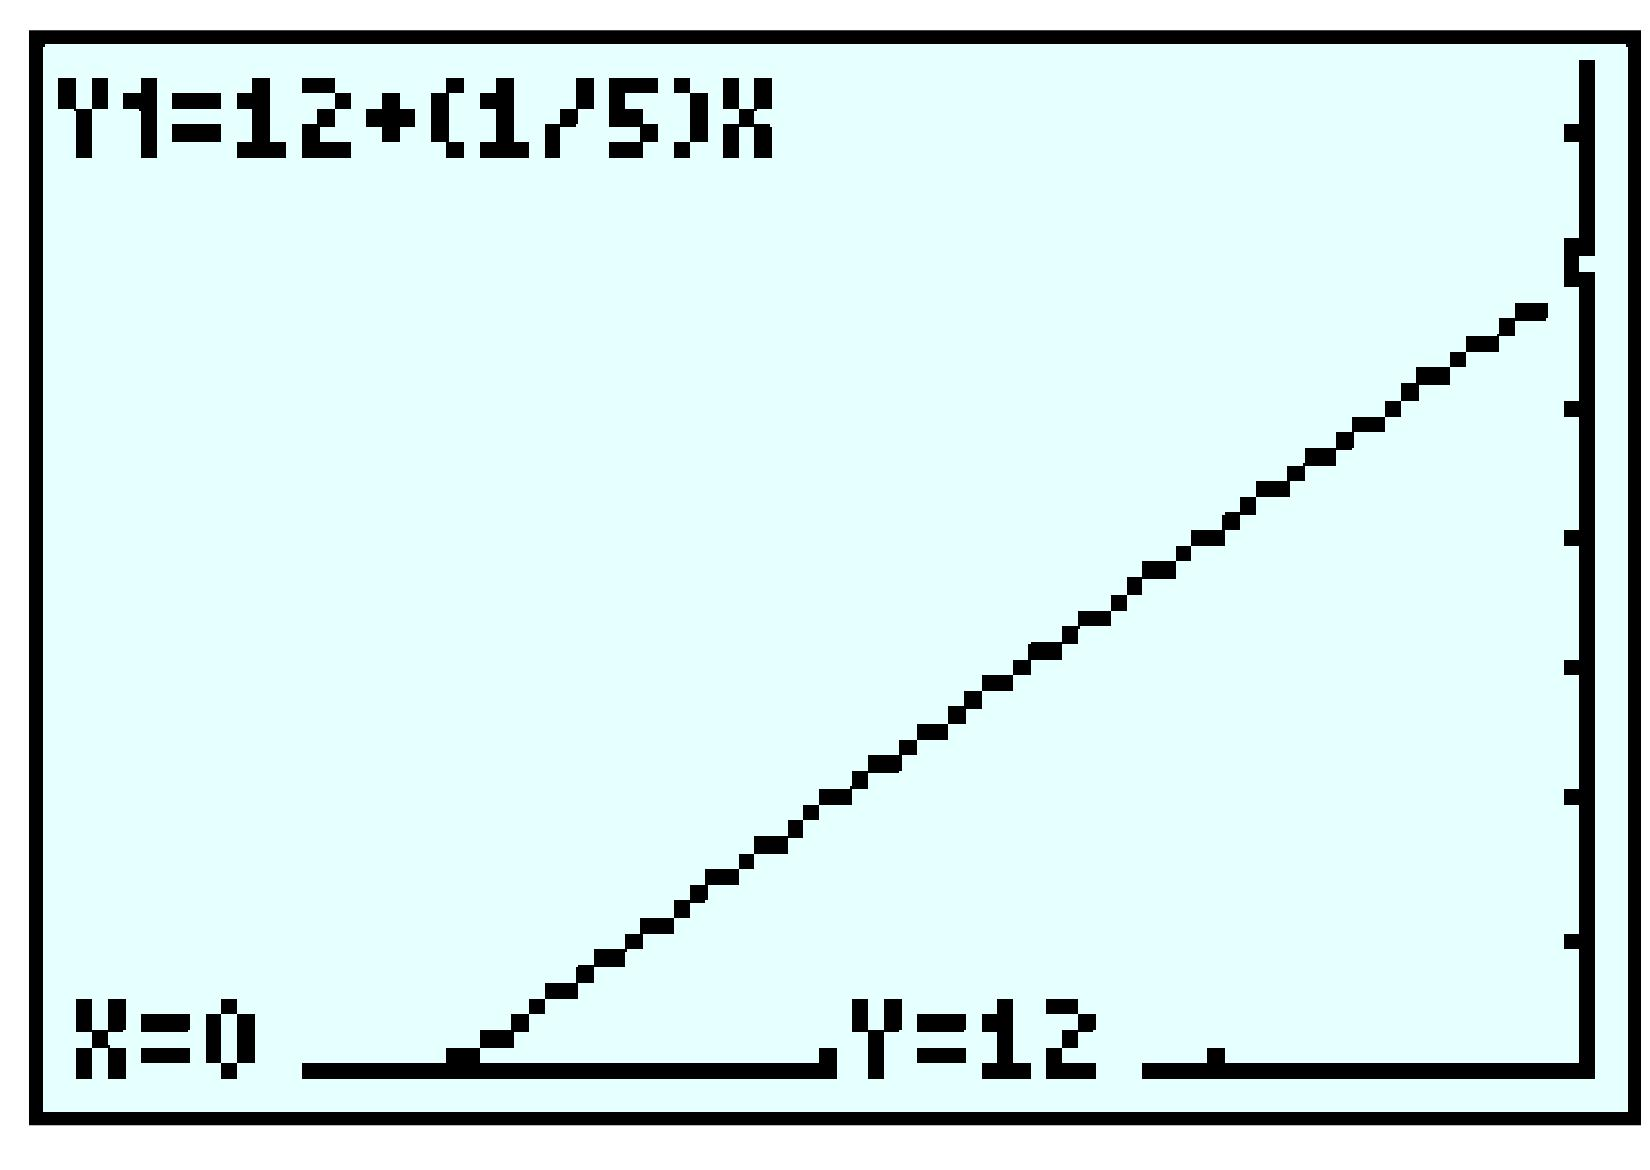
\includegraphics[width=\linewidth]{images/fig-ans-1-1-49.jpg}
\end{sbspanel}%
\end{sidebyside}%
%
\end{enumerate}
%
\end{divisionsolutionegcol}%
\begin{divisionsolutionegcol}{1.1.7.50}{}{g:exercise:idm93552016512}%
\(\dfrac{x}{80} + \dfrac{y}{400}= 1\)%
\end{divisionsolutionegcol}%
\begin{divisionsolutionegcol}{1.1.7.51}{}{g:exercise:idm93552015440}%
\(-2x = 3y + 84\)%
\par\smallskip%
\noindent\textbf{\blocktitlefont Answer}.\quad{}%
\begin{enumerate}[label=\alph*]
\item{}\((-42, 0), (0, -28)\)%
\item{}\(y = \dfrac{-2}{3}x-28\)%
\item{}\begin{sidebyside}{1}{0}{0.3}{0}%
\begin{sbspanel}{0.7}%
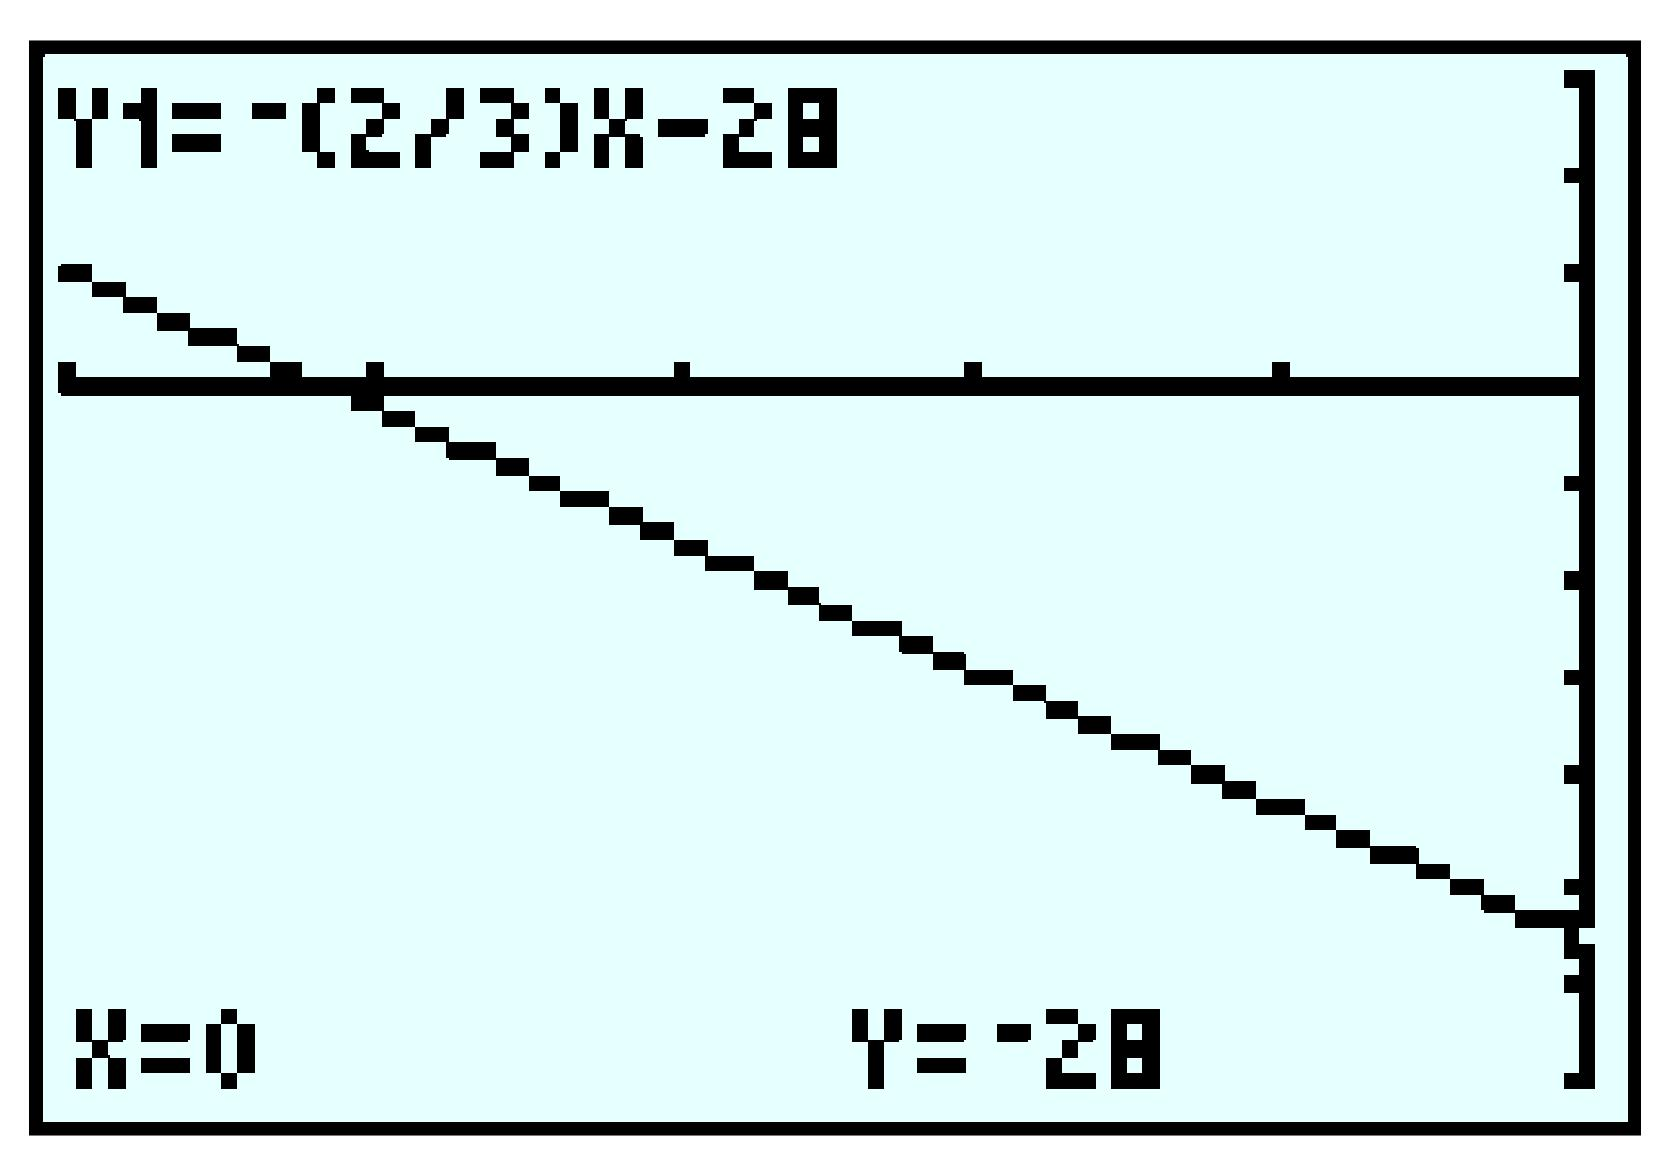
\includegraphics[width=\linewidth]{images/fig-ans-1-1-51.jpg}
\end{sbspanel}%
\end{sidebyside}%
%
\end{enumerate}
%
\end{divisionsolutionegcol}%
\begin{divisionsolutionegcol}{1.1.7.52}{}{g:exercise:idm93552010240}%
\(7x = 91 - 13y\)%
\end{divisionsolutionegcol}%
\end{exercisegroupcol}
\par\medskip\noindent
\section*{1.2 Functions}
\addcontentsline{toc}{section}{1.2 Functions}
\sectionmark{1.2 Functions}
\subsection*{1.2.1 Definition of Function}
\addcontentsline{toc}{subsection}{1.2.1 Definition of Function}
\begin{inlineexercisesolution}{1.2.3}{}{g:exercise:idm93551965072}
%
\begin{enumerate}[label=\alph*]
\item{}As part of a project to improve the success rate of freshmen, the counseling department studied the grades earned by a group of students in English and algebra. Do you think that a student’s grade in algebra is a function of his or her grade in English? Explain why or why not.%
\item{}Phatburger features a soda bar, where you can serve your own soft drinks in any size. Do you think that the number of calories in a serving of Zap Kola is a function of the number of fluid ounces? Explain why or why not.%
\end{enumerate}
%
\par\smallskip%
\noindent\textbf{\blocktitlefont Answer}.\quad{}%
\begin{enumerate}[label=\alph*]
\item{}No, students with the same grade in English can have different grades in algebra.%
\item{}Yes, the number of calories is proportional to the number of fluid ounces.%
\end{enumerate}
%
\end{inlineexercisesolution}
\subsection*{1.2.2 Functions Defined by Tables}
\addcontentsline{toc}{subsection}{1.2.2 Functions Defined by Tables}
\begin{inlineexercisesolution}{1.2.5}{}{g:exercise:idm93551898224}
Decide whether each table describes \(y\) as a function of \(x\). Explain your choice.%
\begin{enumerate}[label=\alph*]
\item{}\begin{sidebyside}{1}{0}{0.37}{0}%
\begin{sbspanel}{0.63}%
{\centering%
{\tabularfont%
\begin{tabular}{AcAcAcAcAcAcAcAcAcA}\hrulethick
\(x\)&\(3.5\)&\(2.0\)&\(2.5\)&\(3.5\)&\(2.5\)&\(4.0\)&\(2.5\)&\(3.0\)\tabularnewline\hrulethin
\(y\)&\(2.5\)&\(3.0\)&\(2.5\)&\(4.0\)&\(3.5\)&\(4.0\)&\(2.0\)&\(2.5\)\tabularnewline\hrulethin
\end{tabular}
}%
\par}
\end{sbspanel}%
\end{sidebyside}%
%
\item{}\begin{sidebyside}{1}{0}{0.5}{0}%
\begin{sbspanel}{0.5}%
{\centering%
{\tabularfont%
\begin{tabular}{AcAcAcAcAcAcAcAcA}\hrulethick
\(x\)&\(-3\)&\(-2\)&\(-1\)&\(0\)&\(1\)&\(2\)&\(3\)\tabularnewline\hrulethin
\(y\)&\(17\)&\(3\)&\(0\)&\(-1\)&\(0\)&\(3\)&\(17\)\tabularnewline\hrulethin
\end{tabular}
}%
\par}
\end{sbspanel}%
\end{sidebyside}%
%
\end{enumerate}
%
\par\smallskip%
\noindent\textbf{\blocktitlefont Answer}.\quad{}%
\begin{enumerate}[label=\alph*]
\item{}No, for example, \(x = 3.5\) corresponds both to \(y = 2.5\) and also to \(y = 4.0\).%
\item{}Yes, each value of \(x\) has exactly one value of \(y\) associated with it.%
\end{enumerate}
%
\end{inlineexercisesolution}
\subsection*{1.2.3 Functions Defined by Graphs}
\addcontentsline{toc}{subsection}{1.2.3 Functions Defined by Graphs}
\begin{inlineexercisesolution}{1.2.7}{}{g:exercise:idm93550779312}
The graph shows the elevation in feet, \(a\), of the Los Angeles Marathon course at a distance \(d\) miles into the race. (Source: \emph{Los Angeles Times}, March 3, 2005)%
\begin{sidebyside}{1}{0.1}{0.1}{0}%
\begin{sbspanel}{0.8}%
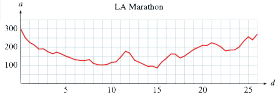
\includegraphics[width=\linewidth]{images/fig-LA-marathon}
\end{sbspanel}%
\end{sidebyside}%
\par
%
\begin{enumerate}[label=\alph*]
\item{}Which variable is the input, and which is the output?%
\item{}What is the elevation at mile 20?%
\item{}At what distances is the elevation 150 feet?%
\item{}What are the maximum and minimum values of \(a\), and when do these values occur?%
\item{}The runners pass by the Los Angeles Coliseum at about 4.2 miles into the race. What is the elevation there?%
\end{enumerate}
%
\par\smallskip%
\noindent\textbf{\blocktitlefont Answer}.\quad{}%
\begin{enumerate}[label=\alph*]
\item{}The input variable is \(d\), and the output variable is \(a\).%
\item{}Approximately \(210\) feet%
\item{}Approximately where \(d\approx 5\), \(d\approx 11\), \(d\approx 12\), \(d\approx 16\), \(d\approx 17.5\), and \(d\approx 18\)%
\item{}The maximum value of \(300\) feet occurs at the start, when \(d = 0\). The minimum of \(85\) feet occurs when \(d\approx 15\).%
\item{}Approximately \(165\) feet%
\end{enumerate}
%
\end{inlineexercisesolution}
\subsection*{1.2.4 Functions Defined by Equations}
\addcontentsline{toc}{subsection}{1.2.4 Functions Defined by Equations}
\begin{inlineexercisesolution}{1.2.9}{}{g:exercise:idm93550753072}
Write an equation that gives the volume, \(V\), of a sphere as a function of its radius, \(r\).%
\par\smallskip%
\noindent\textbf{\blocktitlefont Answer}.\quad{}\(V = \dfrac{4}{3}\pi r^3\)%
\end{inlineexercisesolution}
\subsection*{1.2.5 Function Notation}
\addcontentsline{toc}{subsection}{1.2.5 Function Notation}
\begin{inlineexercisesolution}{1.2.13}{}{g:exercise:idm93550717440}
Let \(F\) be the name of the function defined by the graph in Example~1.2.6, the number of hours of daylight in Peoria.%
\begin{enumerate}[label=\alph*]
\item{}Use function notation to state that \(H\) is a function of \(t\).%
\item{}What does the statement \(F(15) = 9.7\) mean in the context of the problem?%
\end{enumerate}
%
\par\smallskip%
\noindent\textbf{\blocktitlefont Answer}.\quad{}%
\begin{enumerate}[label=\alph*]
\item{}\(H = F(t)\)%
\item{}The sun is above the horizon in Peoria for \(9.7\) hours on January 16.%
\end{enumerate}
%
\end{inlineexercisesolution}
\subsection*{1.2.6 Evaluating a Function}
\addcontentsline{toc}{subsection}{1.2.6 Evaluating a Function}
\begin{inlineexercisesolution}{1.2.15}{}{g:exercise:idm93550692800}
When you exercise, your heart rate should increase until it reaches your target heart rate. The table shows target heart rate, \(r = f(a)\), as a function of age.%
\begin{sidebyside}{1}{0}{0}{0}%
\begin{sbspanel}{1}%
{\centering%
{\tabularfont%
\begin{tabular}{AcAcAcAcAcAcAcAcAcAcAcAcA}\hrulethick
\(a\)&\(20\)&\(25\)&\(30\)&\(35\)&\(40\)&\(45\)&\(50\)&\(55\)&\(60\)&\(65\)&\(70\)\tabularnewline\hrulethin
\(r\)&\(150\)&\(146\)&\(142\)&\(139\)&\(135\)&\(131\)&\(127\)&\(124\)&\(120\)&\(116\)&\(112\)\tabularnewline\hrulethin
\end{tabular}
}%
\par}
\end{sbspanel}%
\end{sidebyside}%
\par
%
\begin{enumerate}[label=\alph*]
\item{}Find \(f(25)\) and \(f(50)\).%
\item{}Find a value of \(a\) for which \(f(a) = 135\).%
\end{enumerate}
%
\par\smallskip%
\noindent\textbf{\blocktitlefont Answer}.\quad{}%
\begin{enumerate}[label=\alph*]
\item{}\(f (25) = 146, ~~f (50) = 127\)%
\item{}\(a = 40\)%
\end{enumerate}
%
\end{inlineexercisesolution}
\begin{inlineexercisesolution}{1.2.17}{}{x:exercise:exercise-function-notation}
Complete the table displaying ordered pairs for the function \(f(x) = 5 - x^3\). Evaluate the function to find the corresponding \(f(x)\)-value for each value of \(x\).%
\begin{sidebyside}{1}{0}{0}{0}%
\begin{sbspanel}{1}%
{\centering%
{\tabularfont%
\begin{tabular}{AcAcAl}\crulethick{1-2}
\(x\)&\(f(x)\)&\tabularnewline\crulethin{1-2}
\(-2\)&\(\)&\(f(\alert{-2})=5-(\alert{-2})^3=~\)\tabularnewline\crulethin{1-2}
\(0\)&\(\)&\(f(\alert{0})=5-\alert{0}^3=\)\tabularnewline\crulethin{1-2}
\(1\)&\(\)&\(f(\alert{1})=5-\alert{1}^3=\)\tabularnewline\crulethin{1-2}
\(3\)&\(\)&\(f(\alert{3})=5-\alert{3}^3=\)\tabularnewline\crulethin{1-2}
\end{tabular}
}%
\par}
\end{sbspanel}%
\end{sidebyside}%
\par\smallskip%
\noindent\textbf{\blocktitlefont Answer}.\quad{}\begin{sidebyside}{1}{0}{0}{0}%
\begin{sbspanel}{1}%
{\centering%
{\tabularfont%
\begin{tabular}{AcAcA}\hrulethick
\(x\)&\(f(x)\)\tabularnewline\hrulethin
\(-2\)&\(13 \)\tabularnewline\hrulethin
\(0\)&\(5\)\tabularnewline\hrulethin
\(1\)&\(4\)\tabularnewline\hrulethin
\(3\)&\(-22\)\tabularnewline\hrulethin
\end{tabular}
}%
\par}
\end{sbspanel}%
\end{sidebyside}%
\end{inlineexercisesolution}
\begin{inlineexercisesolution}{1.2.19}{}{g:exercise:idm93550620384}
The volume of a sphere of radius \(r\) centimeters is given by%
\begin{equation*}
V = V(r) = \frac{4}{3}\pi r^3
\end{equation*}
Evaluate \(V(10)\) and explain what it means.%
\par\smallskip%
\noindent\textbf{\blocktitlefont Answer}.\quad{}\(V(10) = 4000\pi/3\approx 4188.79 \text{ cm}^3\) is the volume of a sphere whose radius is \(10\) cm.%
\end{inlineexercisesolution}
\subsection*{1.2.7 Operations with Function Notation}
\addcontentsline{toc}{subsection}{1.2.7 Operations with Function Notation}
\begin{inlineexercisesolution}{1.2.21}{}{g:exercise:idm93550606912}
A spherical balloon has a radius of 10 centimeters.%
\begin{enumerate}[label=\alph*]
\item{}If we increase the radius by \(h\) centimeters, what will the new volume be?%
\item{}If \(h = 2\), how much did the volume increase?%
\end{enumerate}
%
\par\smallskip%
\noindent\textbf{\blocktitlefont Answer}.\quad{}%
\begin{enumerate}[label=\alph*]
\item{}\(V(10 + h) = \dfrac{4}{3}\pi(10 + h)^3 \text{ cm}^3\)%
\item{}By \(3049.44 \text{ cm}^3\)%
\end{enumerate}
%
\end{inlineexercisesolution}
\begin{inlineexercisesolution}{1.2.24}{}{g:exercise:idm93550587376}
Let \(f(x) = x^3 - 1\) and evaluate each expression.%
\begin{enumerate}[label=\alph*]
\item{}\(\displaystyle f(2) + f(3)\)%
\item{}\(\displaystyle f(2 + 3)\)%
\item{}\(\displaystyle 2 f(x) + 3\)%
\end{enumerate}
%
\par\smallskip%
\noindent\textbf{\blocktitlefont Answer}.\quad{}%
\begin{multicols}{3}
\begin{enumerate}[label=\alph*]
\item{}\(33\)%
\item{}\(124\)%
\item{}\(2x^3 + 1\)%
\end{enumerate}
\end{multicols}
%
\end{inlineexercisesolution}
\subsection*{1.2.10 Homework 1.2}
\addcontentsline{toc}{subsection}{1.2.10 Homework 1.2}
For which of Problems 1-6 is the second quantity a function of the first? Explain your answers.%
\begin{exercisegroup}
\begin{divisionsolutioneg}{1.2.10.1}{}{g:exercise:idm93550450128}%
Price of an item; sales tax on the item at 4\%%
\par\smallskip%
\noindent\textbf{\blocktitlefont Answer}.\quad{}Function; the tax is determined by the price of the item.%
\end{divisionsolutioneg}%
\begin{divisionsolutioneg}{1.2.10.2}{}{g:exercise:idm93550448592}%
Time traveled at constant speed; distance traveled%
\end{divisionsolutioneg}%
\begin{divisionsolutioneg}{1.2.10.3}{}{g:exercise:idm93550447632}%
Number of years of education; annual income%
\par\smallskip%
\noindent\textbf{\blocktitlefont Answer}.\quad{}Not a function; incomes may differ for same number of years of education.%
\end{divisionsolutioneg}%
\begin{divisionsolutioneg}{1.2.10.4}{}{g:exercise:idm93550446080}%
Distance flown in an airplane; price of the ticket%
\end{divisionsolutioneg}%
\begin{divisionsolutioneg}{1.2.10.5}{}{g:exercise:idm93550445120}%
Volume of a container of water; the weight of the water%
\par\smallskip%
\noindent\textbf{\blocktitlefont Answer}.\quad{}Function; weight is determined by volume.%
\end{divisionsolutioneg}%
\begin{divisionsolutioneg}{1.2.10.6}{}{g:exercise:idm93550443584}%
Amount of a paycheck; amount of Social Security tax withheld%
\end{divisionsolutioneg}%
\end{exercisegroup}
\par\medskip\noindent
Each of the objects in Problems 7-14 establishes a correspondence between two variables. Suggest appropriate input and output variables and decide whether the relationship is a function.%
\begin{exercisegroupcol}{2}
\begin{divisionsolutionegcol}{1.2.10.7}{}{g:exercise:idm93550441392}%
An itemized grocery receipt%
\par\smallskip%
\noindent\textbf{\blocktitlefont Answer}.\quad{}Input: items purchased; output: price of item. Yes, a function because each item has only one price.%
\end{divisionsolutionegcol}%
\begin{divisionsolutionegcol}{1.2.10.8}{}{g:exercise:idm93550439712}%
An inventory list%
\end{divisionsolutionegcol}%
\begin{divisionsolutionegcol}{1.2.10.9}{}{g:exercise:idm93550438784}%
An index%
\par\smallskip%
\noindent\textbf{\blocktitlefont Answer}.\quad{}Input: topics; output: page or pages on which topic occurs. No, not a function because the same topic may appear in more than one page.%
\end{divisionsolutionegcol}%
\begin{divisionsolutionegcol}{1.2.10.10}{}{g:exercise:idm93550437200}%
A will%
\end{divisionsolutionegcol}%
\begin{divisionsolutionegcol}{1.2.10.11}{}{g:exercise:idm93550436288}%
An instructor's grade book%
\par\smallskip%
\noindent\textbf{\blocktitlefont Answer}.\quad{}Input: students’ names; output: students’ scores on quizzes, tests, etc. No, not a function because the same student can have different grades on different tests.%
\end{divisionsolutionegcol}%
\begin{divisionsolutionegcol}{1.2.10.12}{}{g:exercise:idm93550434656}%
An address book%
\end{divisionsolutionegcol}%
\begin{divisionsolutionegcol}{1.2.10.13}{}{g:exercise:idm93550433744}%
A bathroom scale%
\par\smallskip%
\noindent\textbf{\blocktitlefont Answer}.\quad{}Input: person stepping on scales; output: person's weight. Yes, a function because a person cannot have two different weights at the same time.%
\end{divisionsolutionegcol}%
\begin{divisionsolutionegcol}{1.2.10.14}{}{g:exercise:idm93550432144}%
A radio dial%
\end{divisionsolutionegcol}%
\end{exercisegroupcol}
\par\medskip\noindent
Which of the tables in Problems 15-26 define the second variable as a function of the first variable? Explain why or why not.%
\begin{exercisegroupcol}{4}
\begin{divisionsolutionegcol}{1.2.10.15}{}{g:exercise:idm93550430064}%
\begin{sidebyside}{1}{0}{0}{0}%
\begin{sbspanel}{1}%
{\centering%
{\tabularfont%
\begin{tabular}{AcAcA}\hrulethick
\(x\)&\(t\)\tabularnewline\hrulethin
\(-1\)&\(2\)\tabularnewline\hrulethin
\(0\)&\(9\)\tabularnewline\hrulethin
\(1\)&\(-2\)\tabularnewline\hrulethin
\(0\)&\(-3\)\tabularnewline\hrulethin
\(-1\)&\(5\)\tabularnewline\hrulethin
\end{tabular}
}%
\par}
\end{sbspanel}%
\end{sidebyside}%
\par\smallskip%
\noindent\textbf{\blocktitlefont Answer}.\quad{}No%
\end{divisionsolutionegcol}%
\begin{divisionsolutionegcol}{1.2.10.16}{}{g:exercise:idm93550418128}%
\begin{sidebyside}{1}{0}{0}{0}%
\begin{sbspanel}{1}%
{\centering%
{\tabularfont%
\begin{tabular}{AcAcA}\hrulethick
\(y\)&\(w\)\tabularnewline\hrulethin
\(0\)&\(8\)\tabularnewline\hrulethin
\(1\)&\(12\)\tabularnewline\hrulethin
\(3\)&\(7\)\tabularnewline\hrulethin
\(5\)&\(-3\)\tabularnewline\hrulethin
\(7\)&\(4\)\tabularnewline\hrulethin
\end{tabular}
}%
\par}
\end{sbspanel}%
\end{sidebyside}%
\end{divisionsolutionegcol}%
\begin{divisionsolutionegcol}{1.2.10.17}{}{g:exercise:idm93550406896}%
\begin{sidebyside}{1}{0}{0}{0}%
\begin{sbspanel}{1}%
{\centering%
{\tabularfont%
\begin{tabular}{AcAcA}\hrulethick
\(x\)&\(y\)\tabularnewline\hrulethin
\(-3\)&\(8\)\tabularnewline\hrulethin
\(-2\)&\(3\)\tabularnewline\hrulethin
\(-1\)&\(0\)\tabularnewline\hrulethin
\(0\)&\(-1\)\tabularnewline\hrulethin
\(1\)&\(0\)\tabularnewline\hrulethin
\(2\)&\(3\)\tabularnewline\hrulethin
\(3\)&\(8\)\tabularnewline\hrulethin
\end{tabular}
}%
\par}
\end{sbspanel}%
\end{sidebyside}%
\par\smallskip%
\noindent\textbf{\blocktitlefont Answer}.\quad{}Yes%
\end{divisionsolutionegcol}%
\begin{divisionsolutionegcol}{1.2.10.18}{}{g:exercise:idm93550392288}%
\begin{sidebyside}{1}{0}{0}{0}%
\begin{sbspanel}{1}%
{\centering%
{\tabularfont%
\begin{tabular}{AcAcA}\hrulethick
\(s\)&\(t\)\tabularnewline\hrulethin
\(2\)&\(5\)\tabularnewline\hrulethin
\(4\)&\(10\)\tabularnewline\hrulethin
\(6\)&\(15\)\tabularnewline\hrulethin
\(8\)&\(20\)\tabularnewline\hrulethin
\(6\)&\(25\)\tabularnewline\hrulethin
\(4\)&\(30\)\tabularnewline\hrulethin
\(2\)&\(35\)\tabularnewline\hrulethin
\end{tabular}
}%
\par}
\end{sbspanel}%
\end{sidebyside}%
\end{divisionsolutionegcol}%
\end{exercisegroupcol}
\par\medskip\noindent
\begin{exercisegroupcol}{2}
\begin{divisionsolutionegcol}{1.2.10.19}{}{g:exercise:idm93550377728}%
\begin{sidebyside}{1}{0}{0}{0}%
\begin{sbspanel}{1}%
{\centering%
{\tabularfont%
\begin{tabular}{AcAcAcAcAcAcA}\hrulethick
\(r\)&\(-4\)&\(-2\)&\(0\)&\(2\)&\(4\)\tabularnewline\hrulethin
\(v\)&\(6\)&\(6\)&\(3\)&\(6\)&\(8\)\tabularnewline\hrulethin
\end{tabular}
}%
\par}
\end{sbspanel}%
\end{sidebyside}%
\par\smallskip%
\noindent\textbf{\blocktitlefont Answer}.\quad{}Yes%
\end{divisionsolutionegcol}%
\begin{divisionsolutionegcol}{1.2.10.20}{}{g:exercise:idm93550366944}%
\begin{sidebyside}{1}{0}{0}{0}%
\begin{sbspanel}{1}%
{\centering%
{\tabularfont%
\begin{tabular}{AcAcAcAcAcAcA}\hrulethick
\(p\)&\(-5\)&\(-4\)&\(-3\)&\(-2\)&\(-1\)\tabularnewline\hrulethin
\(d\)&\(-5\)&\(-4\)&\(-3\)&\(-2\)&\(-1\)\tabularnewline\hrulethin
\end{tabular}
}%
\par}
\end{sbspanel}%
\end{sidebyside}%
\end{divisionsolutionegcol}%
\begin{divisionsolutionegcol}{1.2.10.21}{}{g:exercise:idm93550357008}%
\begin{sidebyside}{1}{0}{0}{0}%
\begin{sbspanel}{1}%
{\centering%
{\tabularfont%
\begin{tabular}{AcAcA}\hrulethick
Pressure (\(p\))&Volume (\(v\))\tabularnewline\hrulethin
\(15\)&\(100.0\)\tabularnewline\hrulethin
\(20\)&\(75.0\)\tabularnewline\hrulethin
\(25\)&\(60.0\)\tabularnewline\hrulethin
\(30\)&\(50.0\)\tabularnewline\hrulethin
\(35\)&\(42.8\)\tabularnewline\hrulethin
\(40\)&\(37.5\)\tabularnewline\hrulethin
\(45\)&\(33.3\)\tabularnewline\hrulethin
\(50\)&\(30.0\)\tabularnewline\hrulethin
\end{tabular}
}%
\par}
\end{sbspanel}%
\end{sidebyside}%
\par\smallskip%
\noindent\textbf{\blocktitlefont Answer}.\quad{}Yes%
\end{divisionsolutionegcol}%
\begin{divisionsolutionegcol}{1.2.10.22}{}{g:exercise:idm93550340432}%
\begin{sidebyside}{1}{0}{0}{0}%
\begin{sbspanel}{1}%
{\centering%
{\tabularfont%
\begin{tabular}{AcAcA}\hrulethick
Frequency (\(f\))&Wavelength (\(w\))\tabularnewline\hrulethin
\(5\)&\(60.0\)\tabularnewline\hrulethin
\(10\)&\(30.0\)\tabularnewline\hrulethin
\(20\)&\(15.0\)\tabularnewline\hrulethin
\(30\)&\(10.0\)\tabularnewline\hrulethin
\(40\)&\(7.5\)\tabularnewline\hrulethin
\(50\)&\(6.0\)\tabularnewline\hrulethin
\(60\)&\(5.0\)\tabularnewline\hrulethin
\(70\)&\(4.3\)\tabularnewline\hrulethin
\end{tabular}
}%
\par}
\end{sbspanel}%
\end{sidebyside}%
\end{divisionsolutionegcol}%
\begin{divisionsolutionegcol}{1.2.10.23}{}{g:exercise:idm93550324384}%
\begin{sidebyside}{1}{0}{0}{0}%
\begin{sbspanel}{1}%
{\centering%
{\tabularfont%
\begin{tabular}{AcAcA}\hrulethick
Temperature (\(T\))&Humidity (\(h\))\tabularnewline\hrulethin
Jan. 1 \(\hphantom{000}34\degree\)F&\(42\%\)\tabularnewline\hrulethin
Jan. 2 \(\hphantom{000}36\degree\)F&\(44\%\)\tabularnewline\hrulethin
Jan. 3 \(\hphantom{000}35\degree\)F&\(47\%\)\tabularnewline\hrulethin
Jan. 4 \(\hphantom{000}29\degree\)F&\(50\%\)\tabularnewline\hrulethin
Jan. 5 \(\hphantom{000}31\degree\)F&\(52\%\)\tabularnewline\hrulethin
Jan. 6 \(\hphantom{000}35\degree\)F&\(51\%\)\tabularnewline\hrulethin
Jan. 7 \(\hphantom{000}34\degree\)F&\(49\%\)\tabularnewline\hrulethin
\end{tabular}
}%
\par}
\end{sbspanel}%
\end{sidebyside}%
\par\smallskip%
\noindent\textbf{\blocktitlefont Answer}.\quad{}No%
\end{divisionsolutionegcol}%
\begin{divisionsolutionegcol}{1.2.10.24}{}{g:exercise:idm93550307232}%
\begin{sidebyside}{1}{0}{0}{0}%
\begin{sbspanel}{1}%
{\centering%
{\tabularfont%
\begin{tabular}{AcAcA}\hrulethick
\tablecelllines{c}{m}
{Inflation\\
rate (\(I\))}
&\tablecelllines{c}{m}
{Unemployment\\
rate (\(U\))}
\tabularnewline\hrulethin
1972 \(\hphantom{000}5.6\%\)&\(5.1\%\)\tabularnewline\hrulethin
1973 \(\hphantom{000}6.2\%\)&\(4.5\%\)\tabularnewline\hrulethin
1974 \(\hphantom{000}10.1\%\)&\(4.9\%\)\tabularnewline\hrulethin
1975 \(\hphantom{000}9.2\%\)&\(7.4\%\)\tabularnewline\hrulethin
1976 \(\hphantom{000}5.8\%\)&\(6.7\%\)\tabularnewline\hrulethin
1977 \(\hphantom{000}5.6\%\)&\(6.8\%\)\tabularnewline\hrulethin
1978 \(\hphantom{000}6.7\%\)&\(7.4\%\)\tabularnewline\hrulethin
\end{tabular}
}%
\par}
\end{sbspanel}%
\end{sidebyside}%
\end{divisionsolutionegcol}%
\begin{divisionsolutionegcol}{1.2.10.25}{}{g:exercise:idm93550290832}%
\begin{sidebyside}{1}{0}{0}{0}%
\begin{sbspanel}{1}%
{\centering%
{\tabularfont%
\begin{tabular}{AcAcA}\hrulethick
\tablecelllines{c}{m}
{Adjusted gross\\
income (\(I\))}
&Tax bracket (\(T\))\tabularnewline\hrulethin
\textdollar{}\(0-2479\)&\(0\%\)\tabularnewline\hrulethin
\textdollar{}\(2480-3669\)&\(4.5\%\)\tabularnewline\hrulethin
\textdollar{}\(3670-4749\)&\(12\%\)\tabularnewline\hrulethin
\textdollar{}\(4750-7009\)&\(14\%\)\tabularnewline\hrulethin
\textdollar{}\(7010-9169\)&\(15\%\)\tabularnewline\hrulethin
\textdollar{}\(9170-11,649\)&\(16\%\)\tabularnewline\hrulethin
\textdollar{}\(11,650-13,919\)&\(18\%\)\tabularnewline\hrulethin
\end{tabular}
}%
\par}
\end{sbspanel}%
\end{sidebyside}%
\par\smallskip%
\noindent\textbf{\blocktitlefont Answer}.\quad{}Yes%
\end{divisionsolutionegcol}%
\begin{divisionsolutionegcol}{1.2.10.26}{}{g:exercise:idm93550274400}%
\begin{sidebyside}{1}{0}{0}{0}%
\begin{sbspanel}{1}%
{\centering%
{\tabularfont%
\begin{tabular}{AcAcA}\hrulethick
\tablecelllines{c}{m}
{Cost of\\
merchandise (\(M\))}
&\tablecelllines{c}{m}
{Shipping\\
charge  (\(C\))}
\tabularnewline\hrulethin
\(\$0.01-10.00\)&\(\$2.50\)\tabularnewline\hrulethin
\(10.01-20.00\)&\(3.75\)\tabularnewline\hrulethin
\(20.01-35.00\)&\(4.85\)\tabularnewline\hrulethin
\(35.01-50.00\)&\(5.95\)\tabularnewline\hrulethin
\(50.01-75.00\)&\(6.95\)\tabularnewline\hrulethin
\(75.01-100.00\)&\(7.95\)\tabularnewline\hrulethin
Over \(100.00\)&\(8.95\)\tabularnewline\hrulethin
\end{tabular}
}%
\par}
\end{sbspanel}%
\end{sidebyside}%
\end{divisionsolutionegcol}%
\end{exercisegroupcol}
\par\medskip\noindent
\begin{divisionsolution}{1.2.10.27}{}{g:exercise:idm93550258832}%
The function described in Problem 21 is called \(g\), so that \(v = g( p)\). Find the following:%
\begin{enumerate}[label=\alph*]
\item{}\(g(25)\)%
\item{}\(g(40)\)%
\item{}\(x\) so that \(g(x) = 50\)%
\end{enumerate}
%
\par\smallskip%
\noindent\textbf{\blocktitlefont Answer}.\quad{}%
\begin{enumerate}[label=\alph*]
\item{}\(60\)%
\item{}\(37.5\)%
\item{}\(30\)%
\end{enumerate}
%
\end{divisionsolution}%
\begin{divisionsolution}{1.2.10.28}{}{g:exercise:idm93550250912}%
The function described in Problem 22 is called \(h\), so that \(w = h( f)\). Find the following:%
\begin{enumerate}[label=\alph*]
\item{}\(h(20)\)%
\item{}\(h(60)\)%
\item{}\(x\) so that \(h(x) = 10\)%
\end{enumerate}
%
\end{divisionsolution}%
\begin{divisionsolution}{1.2.10.29}{}{g:exercise:idm93550246112}%
The function described in Problem 25 is called \(T\), so that \(T = T( I)\). Find the following:%
\begin{enumerate}[label=\alph*]
\item{}\(T(8750)\)%
\item{}\(T(6249)\)%
\item{}\(x\) so that \(T(x) = 15\%\)%
\end{enumerate}
%
\par\smallskip%
\noindent\textbf{\blocktitlefont Answer}.\quad{}%
\begin{enumerate}[label=\alph*]
\item{}\(15\%\)%
\item{}\(14\%\)%
\item{}\textdollar{}7010\textendash{}\textdollar{}9169%
\end{enumerate}
%
\end{divisionsolution}%
\begin{divisionsolution}{1.2.10.30}{}{g:exercise:idm93550238048}%
The function described in Problem 26 is called \(C\), so that \(C = C( M)\). Find the following:%
\begin{enumerate}[label=\alph*]
\item{}\(C(11.50)\)%
\item{}\(C(47.24)\)%
\item{}\(x\) so that \(C(x) = 7.95\)%
\end{enumerate}
%
\end{divisionsolution}%
\begin{divisionsolution}{1.2.10.31}{}{g:exercise:idm93550233248}%
Data indicate that U.S. women are delaying having children longer than their counterparts 50 years ago. The table shows \(f(t)\) the percent of 20\textendash{}24-year-old women in year \(t\) who had not yet had children. (Source: U.S. Dept of Health and Human Services)%
\begin{sidebyside}{1}{0}{0}{0}%
\begin{sbspanel}{1}%
{\centering%
{\tabularfont%
\begin{tabular}{AcAcAcAcAcAcAcAcAcAcA}\hrulethick
Year (\(t\))&\(1960\)&\(1965\)&\(1970\)&\(1975\)&\(1980\)&\(1985\)&\(1990\)&\(1995\)&\(2000\)\tabularnewline\hrulethin
\tablecelllines{c}{m}
{Percent of\\
women}
&\(47.5\)&\(51.4\)&\(47.0\)&\(62.5\)&\(66.2\)&\(67.7\)&\(68.3\)&\(65.5\)&\(66.0\)\tabularnewline\hrulethin
\end{tabular}
}%
\par}
\end{sbspanel}%
\end{sidebyside}%
\par
%
\begin{enumerate}[label=\alph*]
\item{}Evaluate \(f (1985)\) and explain what it means.%
\item{}Estimate a solution to the equation \(f (t) = 68\) and explain what it means.%
\item{}In 1997, \(64.9\%\) of 20\textendash{}24-year-old women had not yet had children. Write an equation with function notation that states this fact.%
\end{enumerate}
%
\par\smallskip%
\noindent\textbf{\blocktitlefont Answer}.\quad{}%
\begin{enumerate}[label=\alph*]
\item{}\(67.7\): In 1985, \(67.7\%\) of 20\textendash{}24 year old women had not yet had children.%
\item{}1987: Approximately \(68\%\) of 20\textendash{}24 year old women had not yet had children in 1987.%
\item{}\(f (1997) = 64.9\)%
\end{enumerate}
%
\end{divisionsolution}%
\begin{divisionsolution}{1.2.10.32}{}{g:exercise:idm93550206864}%
The table shows \(f (t)\), the death rate (per 100,000 people) from HIV among 15\textendash{}24-year-olds, and \(g(t)\), the death rate from HIV among 25\textendash{}34-year-olds, for selected years from 1997 to 2002. (Source: U.S. Dept of Health and Human Services)%
\begin{sidebyside}{1}{0}{0}{0}%
\begin{sbspanel}{1}%
{\centering%
{\tabularfont%
\begin{tabular}{AcAcAcAcAcAcAcAcAcAcAcA}\hrulethick
Year&\(1987\)&\(1988\)&\(1989\)&\(1990\)&\(1992\)&\(1994\)&\(1996\)&\(1998\)&\(2000\)&\(2002\)\tabularnewline\hrulethin
15\textendash{}24-year-olds&\(1.3\)&\(1.4\)&\(1.6\)&\(1.5\)&\(1.6\)&\(1.8\)&\(1.1\)&\(0.6\)&\(0.5\)&\(0.4\)\tabularnewline\hrulethin
25\textendash{}34-year-olds&\(11.7\)&\(14.0\)&\(17.9\)&\(19.7\)&\(24.2\)&\(28.6\)&\(19.2\)&\(8.1\)&\(6.1\)&\(4.6\)\tabularnewline\hrulethin
\end{tabular}
}%
\par}
\end{sbspanel}%
\end{sidebyside}%
\par
%
\begin{enumerate}[label=\alph*]
\item{}Evaluate \(f (1995)\) and explain what it means.%
\item{}Find a solution to the equation \(g (t) = 28.6\) and explain what it means.%
\item{}In 1988, the death rate from HIV for 25\textendash{}34-year-olds was \(10\) times the corresponding rate for 15\textendash{}24-year-olds. Write an equation with function notation that states this fact.%
\end{enumerate}
%
\end{divisionsolution}%
\begin{divisionsolution}{1.2.10.33}{}{g:exercise:idm93550175408}%
When you exercise, your heart rate should increase until it reaches your target heart rate. The table shows target heart rate, \(r = f (a)\), as a function of age.%
\begin{sidebyside}{1}{0}{0}{0}%
\begin{sbspanel}{1}%
{\centering%
{\tabularfont%
\begin{tabular}{AcAcAcAcAcAcAcAcAcAcAcAcA}\hrulethick
\(a\)&\(20\)&\(25\)&\(30\)&\(35\)&\(40\)&\(45\)&\(50\)&\(55\)&\(60\)&\(65\)&\(70\)\tabularnewline\hrulethin
\(r\)&\(150\)&\(146\)&\(142\)&\(139\)&\(135\)&\(131\)&\(127\)&\(124\)&\(120\)&\(116\)&\(112\)\tabularnewline\hrulethin
\end{tabular}
}%
\par}
\end{sbspanel}%
\end{sidebyside}%
\par
%
\begin{enumerate}[label=\alph*]
\item{}Does \(f (50) = 2 f (25)\)?%
\item{}Find a value of a for which \(f (a) = 2a\). Is \(f (a) = 2a\) for all values of \(a\)?%
\item{}Is \(r = f (a)\) an increasing function or a decreasing function?%
\end{enumerate}
%
\par\smallskip%
\noindent\textbf{\blocktitlefont Answer}.\quad{}%
\begin{enumerate}[label=\alph*]
\item{}No%
\item{}60; no%
\item{}Decreasing%
\end{enumerate}
%
\end{divisionsolution}%
\begin{divisionsolution}{1.2.10.34}{}{g:exercise:idm93550149056}%
The table shows \(M = f (d)\), the men's Olympic record time, and \(W = g(d)\), the women's Olympic record time, as a function of the length, \(d\), of the race. For example, the women’s record in the 100 meters is 10.62 seconds, and the men’s record in the 800 meters is 1 minute, 42.58 seconds. (Source: www.hickoksports.com)%
\begin{sidebyside}{1}{0}{0}{0}%
\begin{sbspanel}{1}%
{\centering%
{\tabularfont%
\begin{tabular}{AcAcAcAcAcAcAcAcA}\hrulethick
\tablecelllines{c}{m}
{Distance\\
(meters)}
&\(100\)&\(200\)&\(400\)&\(800\)&\(1500\)&\(5000\)&\(10,000\)\tabularnewline\hrulethin
Men&\(9.63\)&\(19.30\)&\(43.03\)&\(1:40.91\)&\(3:32.07\)&\(12:57.82\)&\(27:01.17\)\tabularnewline\hrulethin
Women&\(10.62\)&\(21.34\)&\(48.25\)&\(1:53.43\)&\(3:53.96\)&\(14:26.17\)&\(29:17.45\)\tabularnewline\hrulethin
\end{tabular}
}%
\par}
\end{sbspanel}%
\end{sidebyside}%
\par
%
\begin{enumerate}[label=\alph*]
\item{}Does \(f (800) = 2 f (400)\)? Does \(g(400) = 2g(200)\)?%
\item{}Find a value of \(d\) for which \(f (2d)\lt 2f (d)\). Is there a value of \(d\) for which \(g(2d)\lt 2g(d)\)?%
\end{enumerate}
%
\end{divisionsolution}%
In Problems 35\textemdash{}40, use the graph of the function to answer the questions.%
\begin{exercisegroup}
\begin{divisionsolutioneg}{1.2.10.35}{}{g:exercise:idm93550122672}%
The graph shows \(C\) as a function of \(t\). \(C\) stands for the number of students (in thousands) at State University who consider themselves computer literate, and \(t\) represents time, measured in years since 1990.%
\begin{sidebyside}{1}{0.32}{0.32}{0}%
\begin{sbspanel}{0.36}%
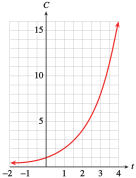
\includegraphics[width=\linewidth]{images/fig-ex-1-2-35}
\end{sbspanel}%
\end{sidebyside}%
\par
%
\begin{enumerate}[label=\alph*]
\item{}When did \(2000\) students consider themselves computer literate?%
\item{}How long did it take that number to double?%
\item{}How long did it take for the number to double again?%
\item{}How many students became computer literate between January 1992 and June 1993?%
\end{enumerate}
%
\par\smallskip%
\noindent\textbf{\blocktitlefont Answer}.\quad{}%
\begin{enumerate}[label=\alph*]
\item{}1991%
\item{}1 yr%
\item{}1 yr%
\item{}About 7300%
\end{enumerate}
%
\end{divisionsolutioneg}%
\begin{divisionsolutioneg}{1.2.10.36}{}{g:exercise:idm93550111952}%
The graph shows \(P\) as a function of \(t\). \(P\) is the number of people in Cedar Grove who owned a portable DVD player \(t\) years after 2000.%
\begin{sidebyside}{1}{0.32}{0.32}{0}%
\begin{sbspanel}{0.36}%
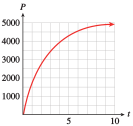
\includegraphics[width=\linewidth]{images/fig-ex-1-2-36}
\end{sbspanel}%
\end{sidebyside}%
%
\begin{enumerate}[label=\alph*]
\item{}When did 3500 people own portable DVD players?%
\item{}How many people owned portable DVD players in 2005?%
\item{}The number of owners of portable DVD players in Cedar Grove seems to be leveling off at what number?%
\item{}How many people acquired portable DVD players between 2001 and 2004?%
\end{enumerate}
\end{divisionsolutioneg}%
\begin{divisionsolutioneg}{1.2.10.37}{}{g:exercise:idm93550104864}%
The graph shows the revenue, \(R\), a movie theater collects as a function of the price, \(d\), it charges for a ticket.%
\begin{sidebyside}{1}{0.3}{0.3}{0}%
\begin{sbspanel}{0.4}%
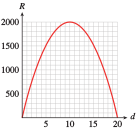
\includegraphics[width=\linewidth]{images/fig-ex-1-2-37}
\end{sbspanel}%
\end{sidebyside}%
%
\begin{enumerate}[label=\alph*]
\item{}What is the revenue if the theater charges \textdollar{}\(12.00\) for a ticket?%
\item{}What should the theater charge for a ticket in order to collect \textdollar{}\(1500\) in revenue?%
\item{}For what values of \(d\) is \(R\gt 1875\)?%
\end{enumerate}
\par\smallskip%
\noindent\textbf{\blocktitlefont Answer}.\quad{}%
\begin{enumerate}[label=\alph*]
\item{}Approximately \textdollar{}\(1920\)%
\item{}\textdollar{}\(5\) or \textdollar{}\(15\)%
\item{}\(7.50\lt d\lt 12.50\)%
\end{enumerate}
%
\end{divisionsolutioneg}%
\begin{divisionsolutioneg}{1.2.10.38}{}{g:exercise:idm93550093904}%
The graph shows \(S\) as a function of \(w\). \(S\) represents the weekly sales of a best-selling book, in thousands of dollars, \(w\) weeks after it is released.%
\begin{sidebyside}{1}{0.3}{0.3}{0}%
\begin{sbspanel}{0.4}%
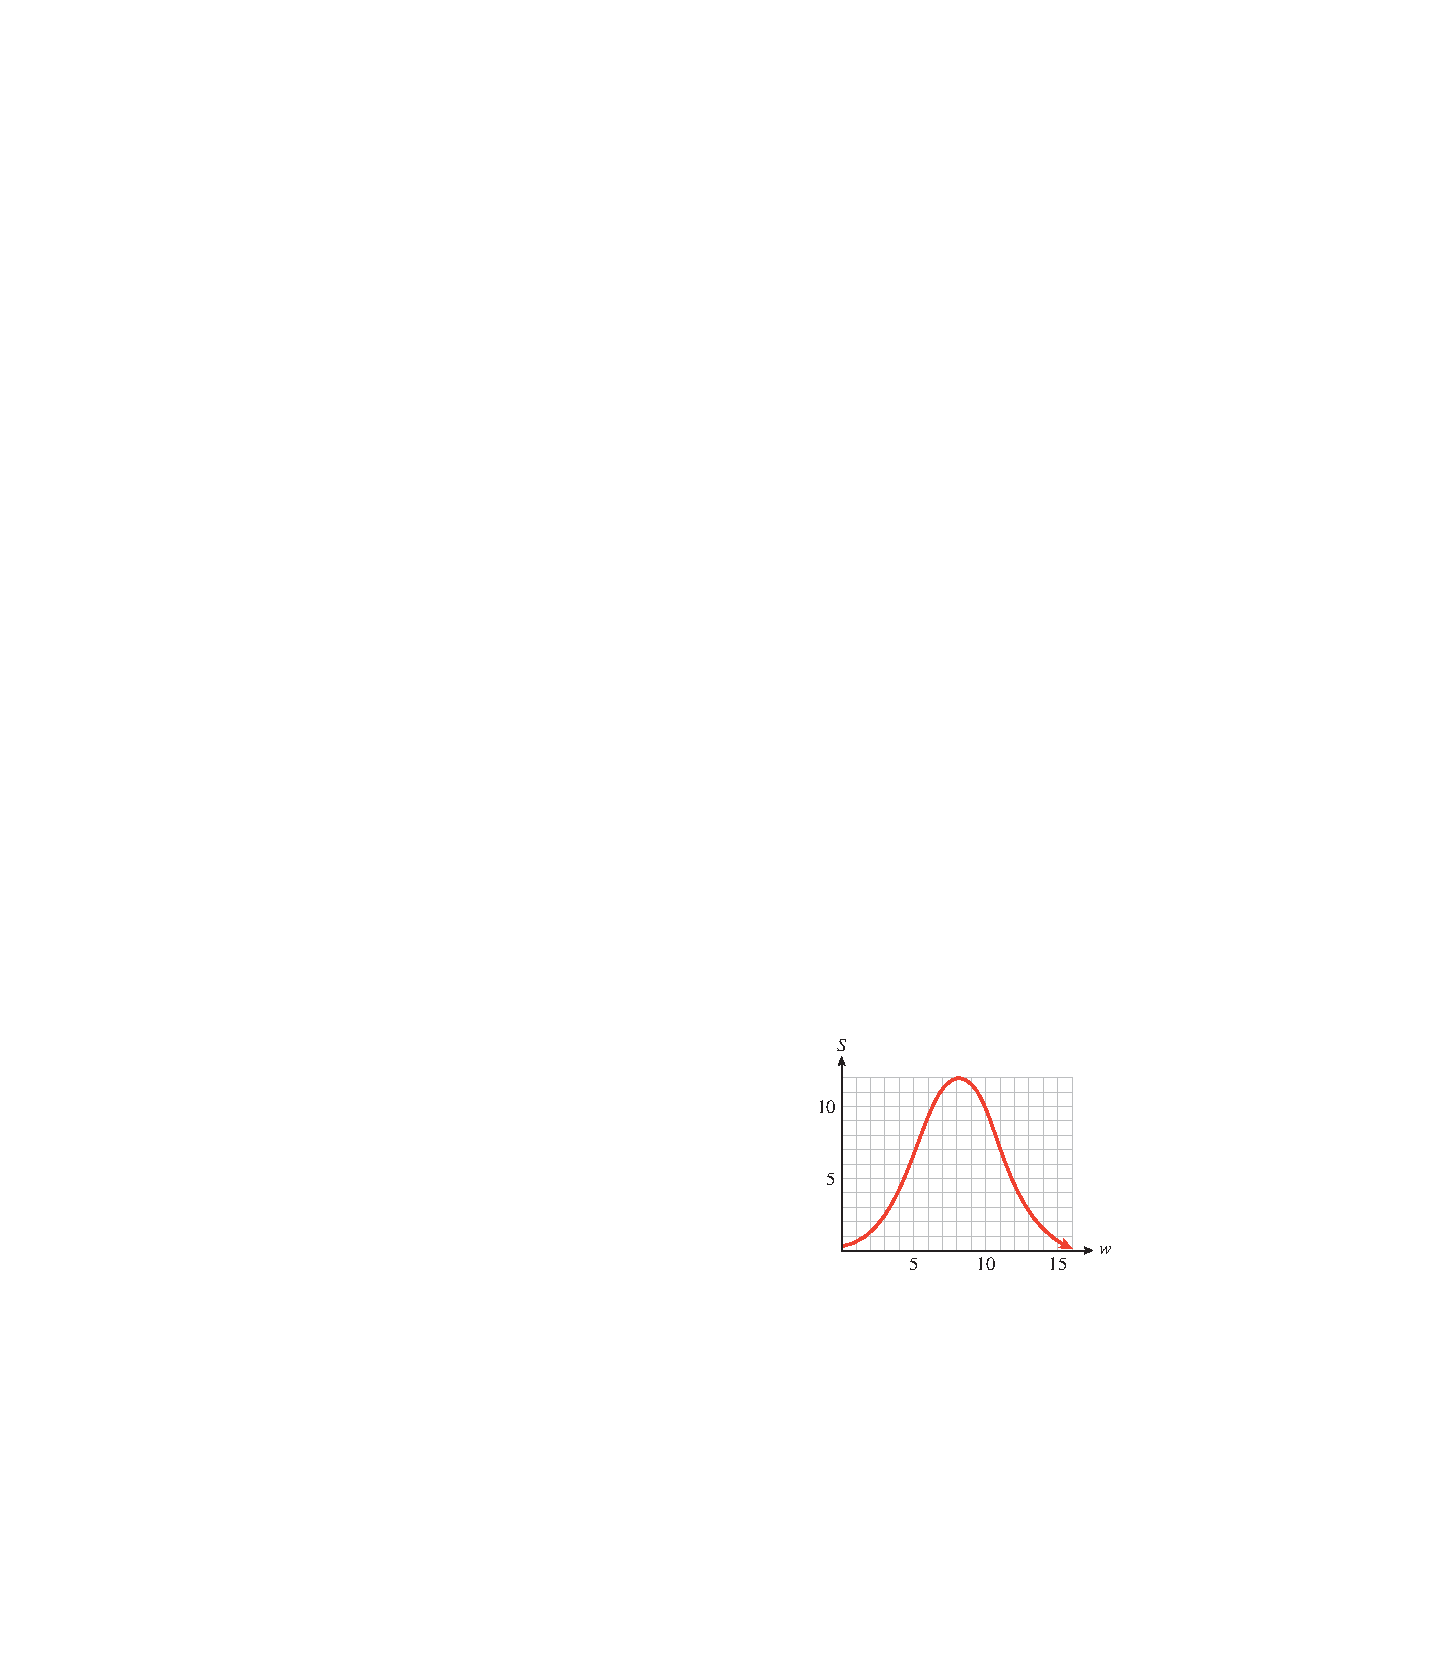
\includegraphics[width=\linewidth]{images/fig-ex-1-2-38}
\end{sbspanel}%
\end{sidebyside}%
%
\begin{enumerate}[label=\alph*]
\item{}In which weeks were sales over \textdollar{}\(7000\)?%
\item{}In which week did sales fall below \textdollar{}\(5000\) on their way down?%
\item{}For what values of \(w\) is \(S\gt 3.4\)?%
\end{enumerate}
\end{divisionsolutioneg}%
\begin{divisionsolutioneg}{1.2.10.39}{}{g:exercise:idm93550085936}%
The graph shows the federal minimum wage, \(M\), as a function of time, \(t\), adjusted for inflation to reflect its buying power in 2004 dollars. (Source: www.infoplease.com)%
\begin{sidebyside}{1}{0}{0}{0}%
\begin{sbspanel}{1}%
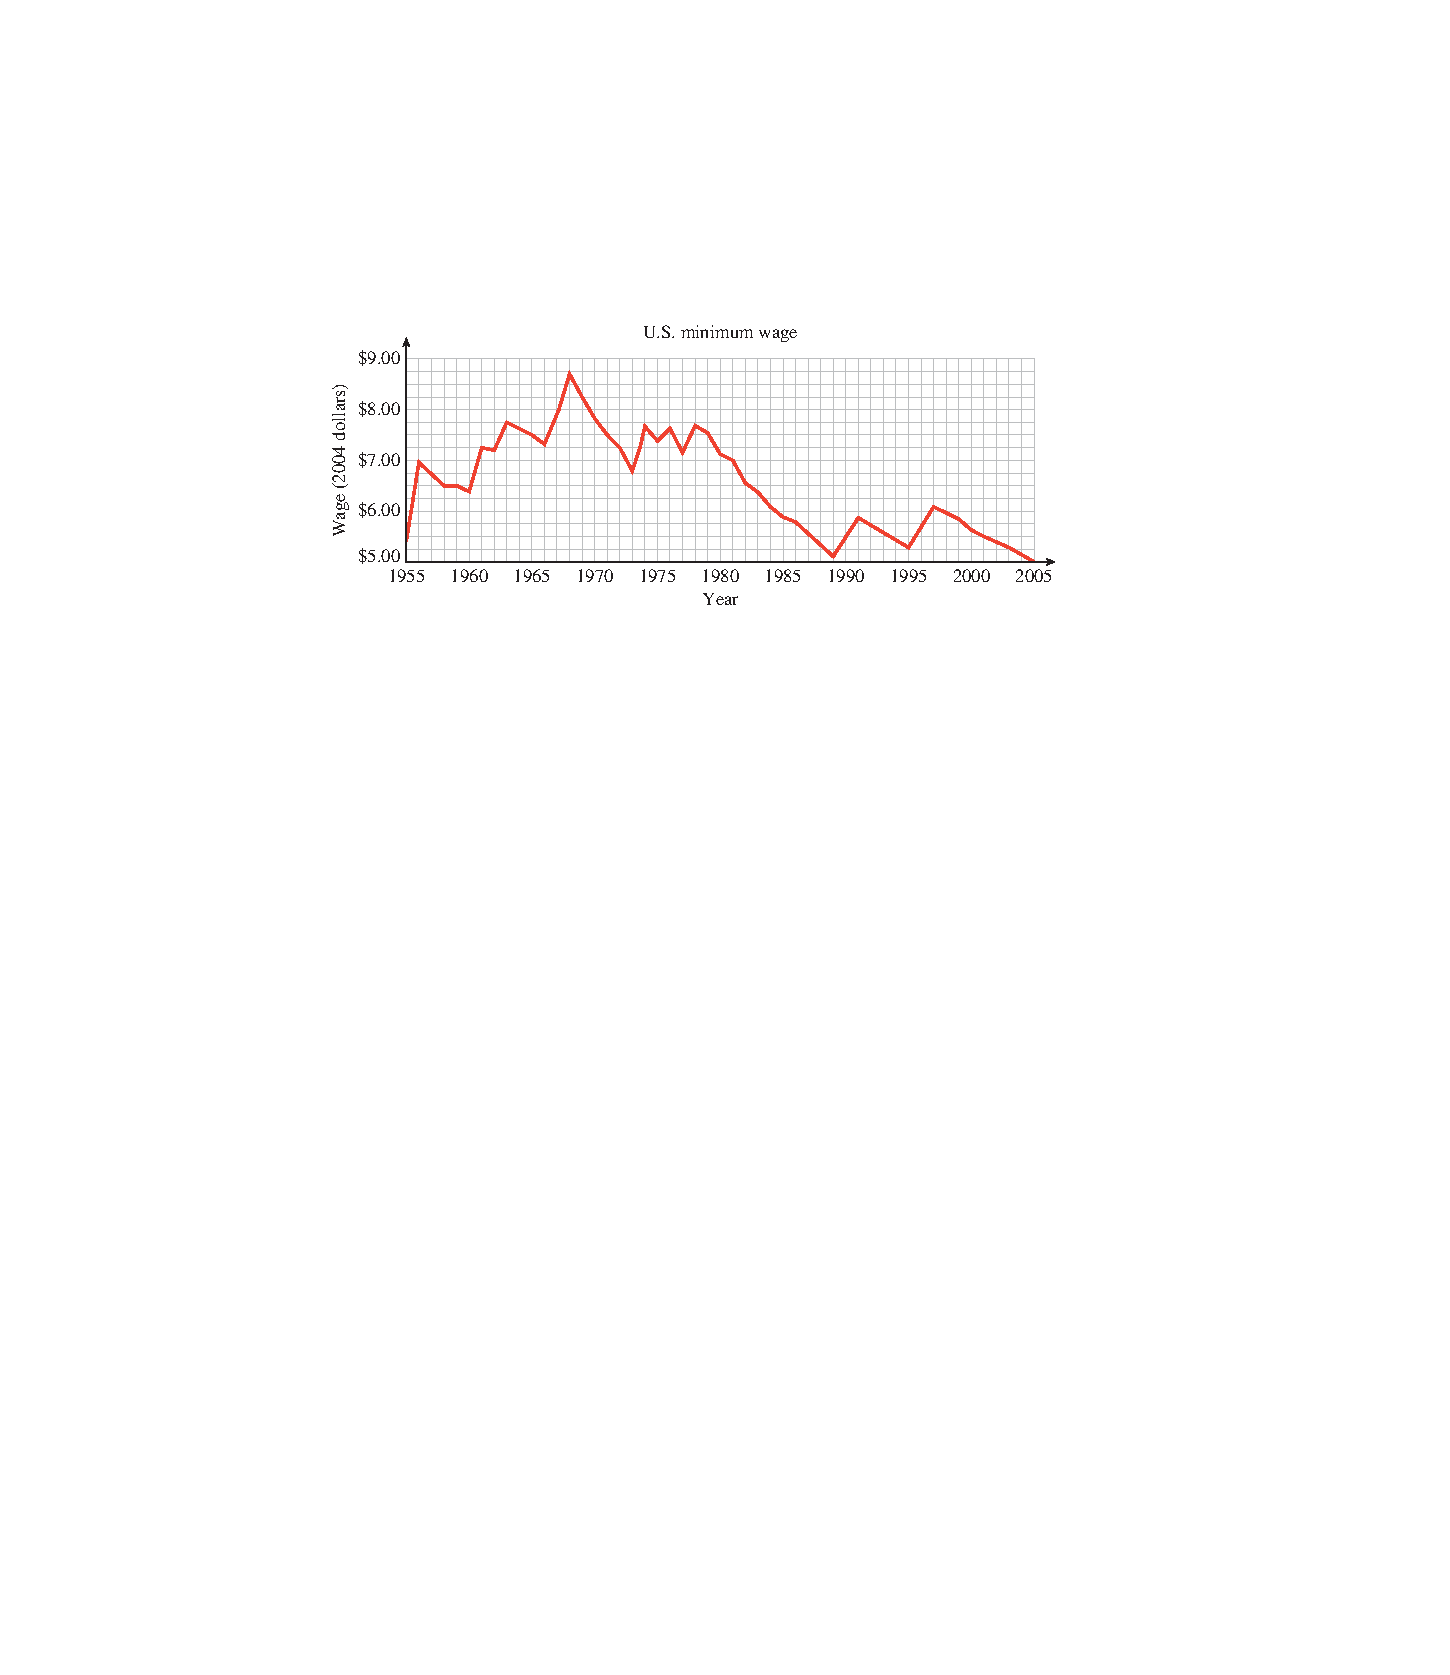
\includegraphics[width=\linewidth]{images/fig-ex-1-2-39}
\end{sbspanel}%
\end{sidebyside}%
\par
%
\begin{enumerate}[label=\alph*]
\item{}When did the minimum wage reach its highest buying power, and what was it worth in 2004 dollars?%
\item{}When did the minimum wage fall to its lowest buying power after its peak, and what was its worth at that time?%
\item{}Give two years in which the minimum wage was worth \textdollar{}\(8\) in 2004 dollars.%
\end{enumerate}
%
\par\smallskip%
\noindent\textbf{\blocktitlefont Answer}.\quad{}%
\begin{enumerate}[label=\alph*]
\item{}1968, about \textdollar{}\(8.70\)%
\item{}1989, about \textdollar{}\(5.10\)%
\item{}1967, approximately 1970%
\end{enumerate}
%
\end{divisionsolutioneg}%
\begin{divisionsolutioneg}{1.2.10.40}{}{g:exercise:idm93550076624}%
The graph shows the U.S. unemployment rate, \(U\), as a function of time, \(t\), for the years 1985\textendash{}2004. (Source: U.S. Bureau of Labor Statistics)%
\begin{sidebyside}{1}{0.2}{0.2}{0}%
\begin{sbspanel}{0.6}%
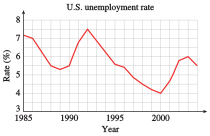
\includegraphics[width=\linewidth]{images/fig-ex-1-2-40}
\end{sbspanel}%
\end{sidebyside}%
\par
%
\begin{enumerate}[label=\alph*]
\item{}When did the unemployment rate reach its highest value, and what was its highest value?%
\item{}When did the unemployment rate fall to its lowest value, and what was its lowest value?%
\item{}Give two years in which the unemployment rate was \(4.5\%\).%
\end{enumerate}
%
\end{divisionsolutioneg}%
\end{exercisegroup}
\par\medskip\noindent
In Problems 41\textendash{}48, evaluate each function for the given values, if possible. If not, state why.%
\begin{exercisegroupcol}{2}
\begin{divisionsolutionegcol}{1.2.10.41}{}{g:exercise:idm93550068144}%
\(f (x) = 6 - 2x\)%
\begin{multicols}{2}
\begin{enumerate}[label=\alph*]
\item{}\(f(3)\)%
\item{}\(f(-2)\)%
\item{}\(f(12.7)\)%
\item{}\(f\left(\dfrac{2}{3}\right)\)%
\end{enumerate}
\end{multicols}
%
\par\smallskip%
\noindent\textbf{\blocktitlefont Answer}.\quad{}%
\begin{multicols}{2}
\begin{enumerate}[label=\alph*]
\item{}\(0\)%
\item{}\(10\)%
\item{}\(-19.4\)%
\item{}\(\dfrac{14}{3} \)%
\end{enumerate}
\end{multicols}
%
\end{divisionsolutionegcol}%
\begin{divisionsolutionegcol}{1.2.10.42}{}{g:exercise:idm93550059392}%
\(g(t) = 5t - 3\)%
\begin{multicols}{2}
\begin{enumerate}[label=\alph*]
\item{}\(g(1)\)%
\item{}\(g(-4)\)%
\item{}\(g(14.1)\)%
\item{}\(g\left(\dfrac{3}{4}\right)\)%
\end{enumerate}
\end{multicols}
%
\end{divisionsolutionegcol}%
\begin{divisionsolutionegcol}{1.2.10.43}{}{g:exercise:idm93550054688}%
\(h(v) = 2v^2 - 3v + 1\)%
\begin{multicols}{2}
\begin{enumerate}[label=\alph*]
\item{}\(h(0)\)%
\item{}\(h(-1)\)%
\item{}\(h\left(\dfrac{1}{4}\right)\)%
\item{}\(h(-6.2)\)%
\end{enumerate}
\end{multicols}
%
\par\smallskip%
\noindent\textbf{\blocktitlefont Answer}.\quad{}%
\begin{multicols}{2}
\begin{enumerate}[label=\alph*]
\item{}\(1\)%
\item{}\(6\)%
\item{}\(\dfrac{3}{8}\)%
\item{}\(96.48 \)%
\end{enumerate}
\end{multicols}
%
\end{divisionsolutionegcol}%
\begin{divisionsolutionegcol}{1.2.10.44}{}{g:exercise:idm93550045920}%
\(r (s) = 2s - s^2\)%
\begin{multicols}{2}
\begin{enumerate}[label=\alph*]
\item{}\(r(2)\)%
\item{}\(r(-4)\)%
\item{}\(r\left(\dfrac{1}{3}\right)\)%
\item{}\(r(-1.3)\)%
\end{enumerate}
\end{multicols}
%
\end{divisionsolutionegcol}%
\begin{divisionsolutionegcol}{1.2.10.45}{}{g:exercise:idm93550041200}%
\(H(z) = \dfrac{2z - 3}{z + 2}\)%
\begin{multicols}{2}
\begin{enumerate}[label=\alph*]
\item{}\(H(4)\)%
\item{}\(H(-3)\)%
\item{}\(H\left(\dfrac{4}{3}\right)\)%
\item{}\(H(4.5)\)%
\end{enumerate}
\end{multicols}
%
\par\smallskip%
\noindent\textbf{\blocktitlefont Answer}.\quad{}%
\begin{multicols}{2}
\begin{enumerate}[label=\alph*]
\item{}\(\dfrac{5}{6} \)%
\item{}\(9\)%
\item{}\(\dfrac{-1}{10}\)%
\item{}\(\dfrac{12}{13}\approx 0.923 \)%
\end{enumerate}
\end{multicols}
%
\end{divisionsolutionegcol}%
\begin{divisionsolutionegcol}{1.2.10.46}{}{g:exercise:idm93550032272}%
\(F(x) = \dfrac{1-x}{2x-3}\)%
\begin{multicols}{2}
\begin{enumerate}[label=\alph*]
\item{}\(F(0)\)%
\item{}\(F(-3)\)%
\item{}\(F\left(\dfrac{5}{2}\right)\)%
\item{}\(F(\dfrac{3}{2})\)%
\end{enumerate}
\end{multicols}
%
\end{divisionsolutionegcol}%
\begin{divisionsolutionegcol}{1.2.10.47}{}{g:exercise:idm93550027552}%
\(E(t) =\sqrt{t-4}\)%
\begin{multicols}{2}
\begin{enumerate}[label=\alph*]
\item{}\(E(16)\)%
\item{}\(E(4)\)%
\item{}\(E(7)\)%
\item{}\(E(4.2)\)%
\end{enumerate}
\end{multicols}
%
\par\smallskip%
\noindent\textbf{\blocktitlefont Answer}.\quad{}%
\begin{multicols}{2}
\begin{enumerate}[label=\alph*]
\item{}\(\sqrt{12} \)%
\item{}\(0\)%
\item{}\(\sqrt{3}\)%
\item{}\(\sqrt{0.2}\approx 0.447 \)%
\end{enumerate}
\end{multicols}
%
\end{divisionsolutionegcol}%
\begin{divisionsolutionegcol}{1.2.10.48}{}{g:exercise:idm93550018784}%
\(D(r) =\sqrt{5-r}\)%
\begin{multicols}{2}
\begin{enumerate}[label=\alph*]
\item{}\(D(4)\)%
\item{}\(D(-3)\)%
\item{}\(D(9)\)%
\item{}\(D(4.6)\)%
\end{enumerate}
\end{multicols}
%
\end{divisionsolutionegcol}%
\end{exercisegroupcol}
\par\medskip\noindent
\begin{divisionsolution}{1.2.10.49}{}{g:exercise:idm93550013936}%
A sport utility vehicle costs \textdollar{}\(28,000\) and depreciates according to the formula%
\begin{equation*}
V(t) = 28,000 (1 - 0.08t)
\end{equation*}
where \(V\) is the value of the vehicle after \(t\) years.%
\begin{enumerate}[label=\alph*]
\item{}Evaluate \(V(12)\) and explain what it means.%
\item{}Solve the equation \(V(t) = 0\) and explain what it means.%
\item{}If this year is \(t = n\), what does \(V(n + 2)\) mean?%
\end{enumerate}
%
\par\smallskip%
\noindent\textbf{\blocktitlefont Answer}.\quad{}%
\begin{enumerate}[label=\alph*]
\item{}\(V(12) = 1120\): After 12 years, the SUV is worth \textdollar{}\(1120\).%
\item{}\(t = 12.5\): The SUV has zero value after \(12\frac{1}{2}\) years.%
\item{}The value 2 years later%
\end{enumerate}
%
\end{divisionsolution}%
\begin{divisionsolution}{1.2.10.50}{}{g:exercise:idm93550003264}%
In a profit-sharing plan, an employee receives a salary of%
\begin{equation*}
S(x) = 20,000 + 0.01x
\end{equation*}
where \(x\) represents the company's profit for the year.%
\begin{enumerate}[label=\alph*]
\item{}Evaluate \(S(850,000)\) and explain what it means.%
\item{}Solve the equation \(S(x) = 30,000\) and explain what it means.%
\item{}If the company made a profit of \(p\) dollars this year, what does \(S(2p)\) mean?%
\end{enumerate}
%
\end{divisionsolution}%
\begin{divisionsolution}{1.2.10.51}{}{g:exercise:idm93549997440}%
The number of compact cars that a large dealership can sell at price \(p\) is given by%
\begin{equation*}
N( p) = \dfrac{12,000,000}{p}
\end{equation*}
%
\begin{enumerate}[label=\alph*]
\item{}Evaluate \(N(6000)\) and explain what it means.%
\item{}As \(p\) increases, does \(N(p)\) increase or decrease? Why is this reasonable?%
\item{}If the current price for a compact car is \(D\), what does \(2N(D)\) mean?%
\end{enumerate}
%
\par\smallskip%
\noindent\textbf{\blocktitlefont Answer}.\quad{}%
\begin{enumerate}[label=\alph*]
\item{}\(N(6000) = 2000\): \(2000\) cars will be sold at a price of \textdollar{}\(6000\).%
\item{}\(N(p)\) decreases with increasing \(p\) because fewer cars will be sold when the price increases.%
\item{}\(2N(D)\) represents twice the number of cars that can be sold at the current price.%
\end{enumerate}
%
\end{divisionsolution}%
\begin{divisionsolution}{1.2.10.52}{}{g:exercise:idm93549986400}%
A department store finds that the market value of its Christmas-related merchandise is given by%
\begin{equation*}
M(t) = \dfrac{600,000}{t},~~ t\le 30
\end{equation*}
where \(t\) is the number of weeks after Christmas.%
\begin{enumerate}[label=\alph*]
\item{}Evaluate \(M(2)\) and explain what it means.%
\item{}As \(t\) increases, does \(M(t)\) increase or decrease? Why is this reasonable?%
\item{}If this week \(t = n\), what does \(M(n + 1)\) mean?%
\end{enumerate}
%
\end{divisionsolution}%
\begin{divisionsolution}{1.2.10.53}{}{g:exercise:idm93549980144}%
The velocity of a car that brakes suddenly can be determined from the length of its skid marks, \(d\), by%
\begin{equation*}
v(d) = \sqrt{12d}
\end{equation*}
where \(d\) is in feet and \(v\) is in miles per hour.%
\begin{enumerate}[label=\alph*]
\item{}Evaluate \(v(250)\) and explain what it means.%
\item{}Estimate the length of the skid marks left by a car traveling at \(100\) miles per hour.%
\item{}Write your answer to part (b) with function notation.%
\end{enumerate}
%
\par\smallskip%
\noindent\textbf{\blocktitlefont Answer}.\quad{}%
\begin{enumerate}[label=\alph*]
\item{}\(v(250) = 54.8\) is the speed of a car that left \(250\)-foot skid marks.%
\item{}\(833\dfrac{1}{3}\) feet%
\item{}\(v\left(833\dfrac{1}{3}\right)= 100\)%
\end{enumerate}
%
\end{divisionsolution}%
\begin{divisionsolution}{1.2.10.54}{}{g:exercise:idm93549970464}%
The distance, \(d\), in miles that a person can see on a clear day from a height, \(h\), in feet is given by%
\begin{equation*}
d(h) = 1.22\sqrt{h}
\end{equation*}
%
\begin{enumerate}[label=\alph*]
\item{}Evaluate \(d(20,320)\) and explain what it means.%
\item{}Estimate the height you need in order to see \(100\) miles.%
\item{}Write your answer to part (b) with function notation.%
\end{enumerate}
%
\end{divisionsolution}%
\begin{divisionsolution}{1.2.10.55}{}{g:exercise:idm93549965232}%
The figure gives data about snowfall, air temperature, and number of avalanches on the Mikka glacier in Sarek, Lapland, in 1957. (Source: Leopold, Wolman, Miller, 1992)%
\begin{sidebyside}{1}{0.1}{0.1}{0}%
\begin{sbspanel}{0.8}%
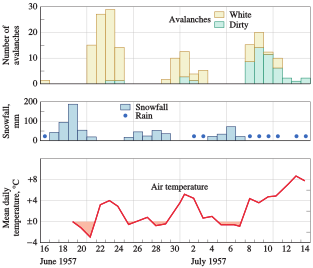
\includegraphics[width=\linewidth]{images/fig-ex-1-2-55}
\end{sbspanel}%
\end{sidebyside}%
\par
%
\begin{enumerate}[label=\alph*]
\item{}During June and July, avalanches occurred over three separate time intervals. What were they?%
\item{}Over what three time intervals did snow fall?%
\item{}When was the temperature above freezing (\(0\degree\)C)?%
\item{}Using your answers to parts (a)\textendash{}(c), make a conjecture about the conditions that encourage avalanches.%
\end{enumerate}
%
\par\smallskip%
\noindent\textbf{\blocktitlefont Answer}.\quad{}%
\begin{enumerate}[label=\alph*]
\item{}June 21\textendash{}24, June 29\textendash{}July 3, July 8\textendash{}14%
\item{}June 17\textendash{}21, June 25\textendash{}29, July 4\textendash{}7%
\item{}June 22\textendash{}24, June 27, June 29\textendash{}July 4, July 8\textendash{}14%
\item{}Avalanches occur when temperatures rise above freezing immediately after snowfall.%
\end{enumerate}
%
\end{divisionsolution}%
\begin{divisionsolution}{1.2.10.56}{}{g:exercise:idm93549953328}%
The bar graph shows the percent of Earth's surface that lies at various altitudes or depths below the surface of the oceans. (Depths are given as negative altitudes.) (Source: Open University)%
\begin{sidebyside}{1}{0.15}{0.15}{0}%
\begin{sbspanel}{0.7}%
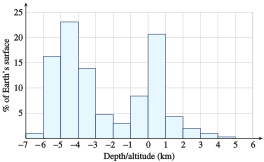
\includegraphics[width=\linewidth]{images/fig-ex-1-2-56}
\end{sbspanel}%
\end{sidebyside}%
\par
%
\begin{enumerate}[label=\alph*]
\item{}Read the graph and complete the table.%
\begin{sidebyside}{1}{0}{0}{0}%
\begin{sbspanel}{1}%
{\centering%
{\tabularfont%
\begin{tabular}{AcAcA}\hrulethick
Altitude (km)&\tablecelllines{c}{m}
{Percent of\\
Earth's surface}
\tabularnewline\hrulethin
\(-7\) to \(-6\)&\(\)\tabularnewline\hrulethin
\(-6\) to \(-5\)&\(\)\tabularnewline\hrulethin
\(-5\) to \(-4\)&\(\)\tabularnewline\hrulethin
\(-4\) to \(-3\)&\(\)\tabularnewline\hrulethin
\(-3\) to \(-2\)&\(\)\tabularnewline\hrulethin
\(-2\) to \(-1\)&\(\)\tabularnewline\hrulethin
\(-1\) to \(0\)&\(\)\tabularnewline\hrulethin
\(0\) to \(1\)&\(\)\tabularnewline\hrulethin
\(1\) to \(2\)&\(\)\tabularnewline\hrulethin
\(2\) to \(3\)&\(\)\tabularnewline\hrulethin
\(3\) to \(4\)&\(\)\tabularnewline\hrulethin
\(4\) to \(5\)&\(\)\tabularnewline\hrulethin
\end{tabular}
}%
\par}
\end{sbspanel}%
\end{sidebyside}%
\item{}What is the most common altitude? What is the second most common altitude??%
\item{}Approximately what percent of the Earth's surface is below sea level?%
\item{}The height of Mt. Everest is \(8.85\) kilometers. Can you think of a reason why it is not included in the graph?%
\end{enumerate}
%
\end{divisionsolution}%
\begin{divisionsolution}{1.2.10.57}{}{g:exercise:idm93549923552}%
The graph shows the temperature of the ocean at various depths. (Source: Open University)%
\begin{sidebyside}{2}{0.035}{0.035}{0.07}%
\begin{sbspanel}{0.36}%
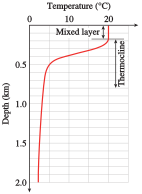
\includegraphics[width=\linewidth]{images/fig-ex-1-2-57}
\end{sbspanel}%
\begin{sbspanel}{0.5}%
%
\begin{enumerate}[label=\alph*]
\item{}Is depth a function of temperature?%
\item{}Is temperature a function of depth?%
\item{}The axes are scaled in an unusual way. Why is it useful to present the graph in this way?%
\end{enumerate}
%
\end{sbspanel}%
\end{sidebyside}%
\par\smallskip%
\noindent\textbf{\blocktitlefont Answer}.\quad{}%
\begin{enumerate}[label=\alph*]
\item{}No%
\item{}Yes%
\item{}Moving downwards on the graph corresponds to moving downwards in the ocean.%
\end{enumerate}
%
\end{divisionsolution}%
\begin{divisionsolution}{1.2.10.58}{}{g:exercise:idm93549916208}%
The graph shows the relationship between annual precipitation, \(p\), in a region and the amount of erosion, measured in tons per square mile, \(s\). (Source: Leopold, Wolman, Miller, 1992)%
\begin{sidebyside}{1}{0.25}{0.25}{0}%
\begin{sbspanel}{0.5}%
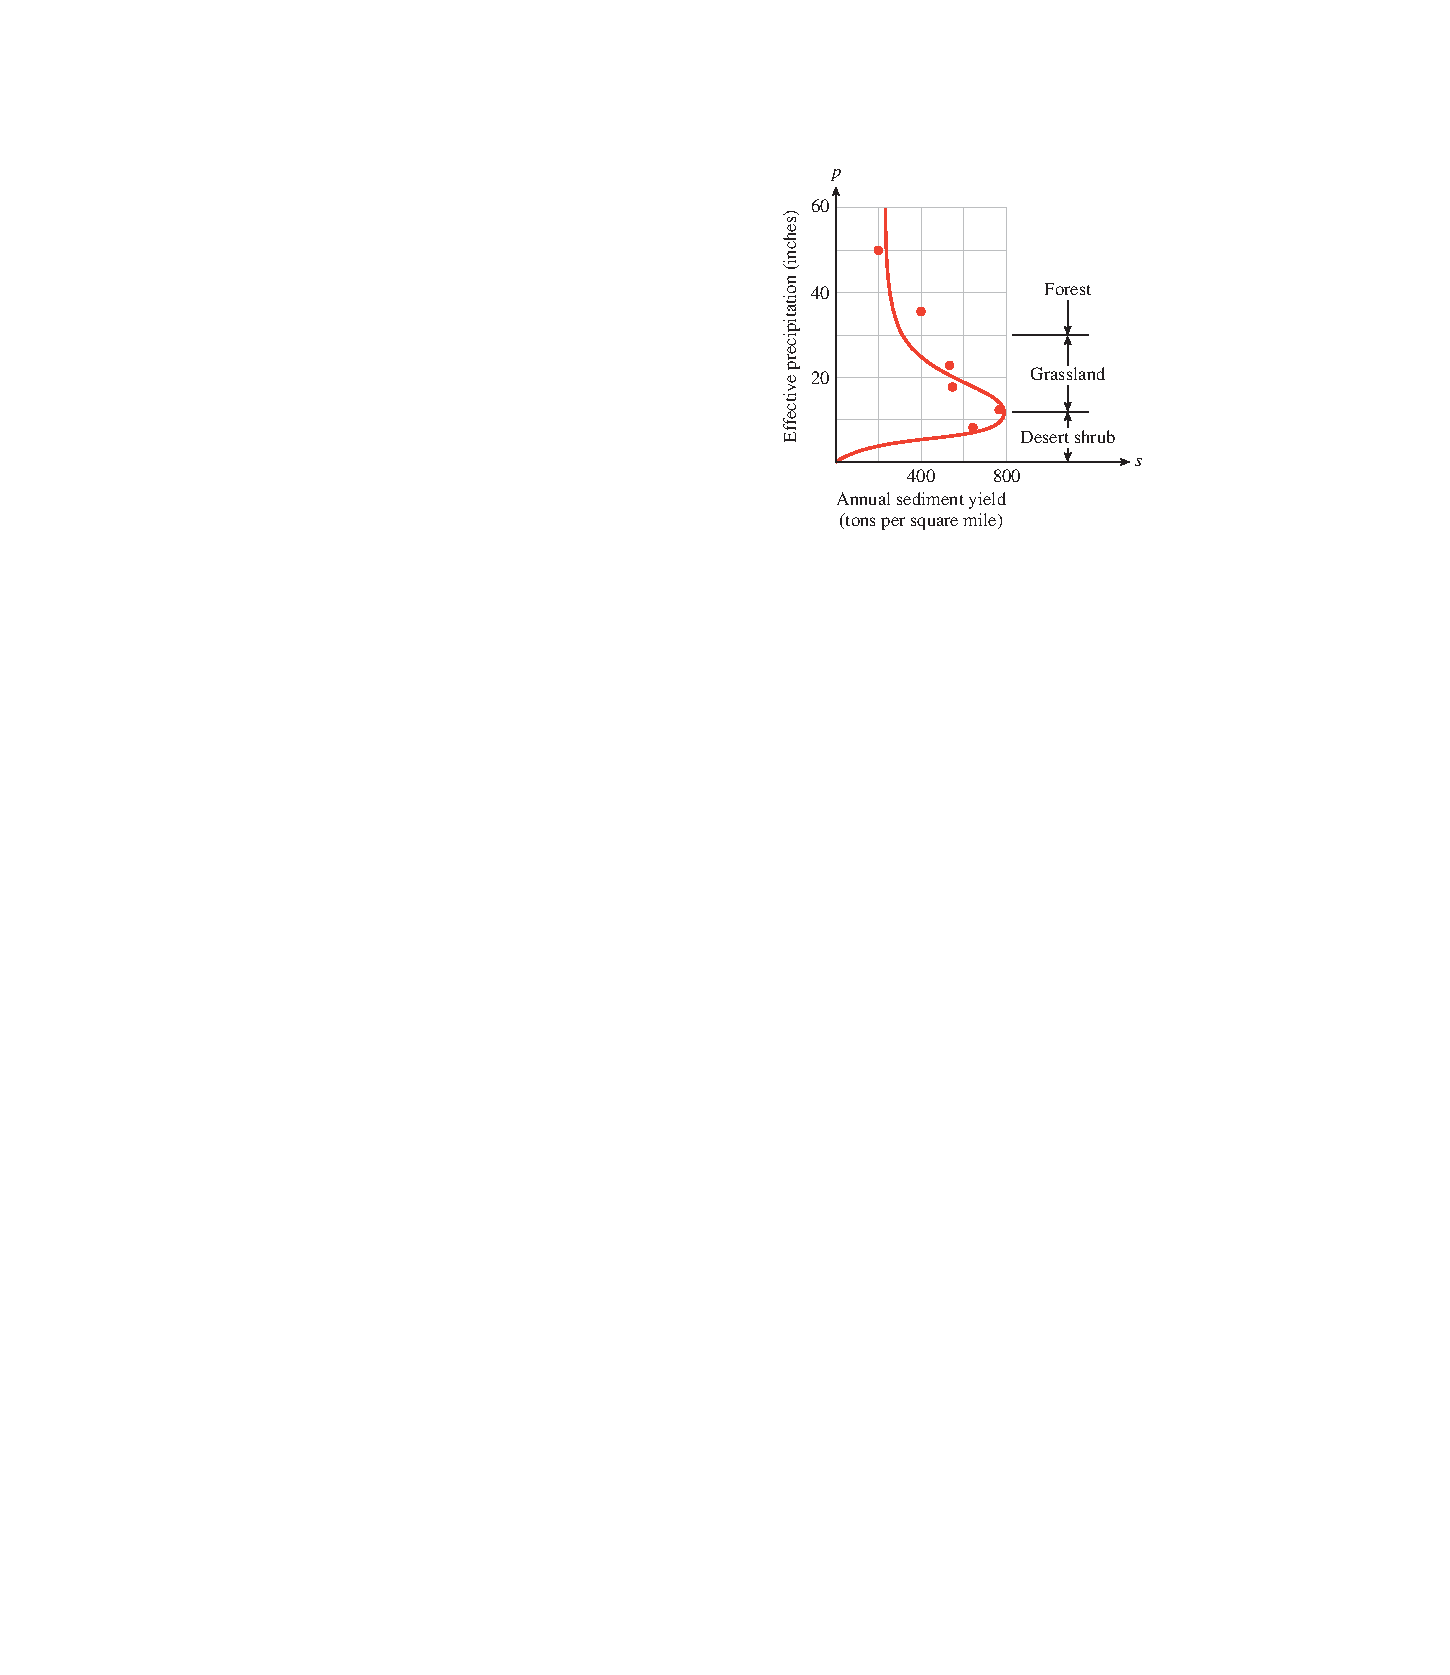
\includegraphics[width=\linewidth]{images/fig-ex-1-2-58}
\end{sbspanel}%
\end{sidebyside}%
\par
%
\begin{enumerate}[label=\alph*]
\item{}Is the amount of erosion a function of the amount of precipitation?%
\item{}At what annual precipitation is erosion at a maximum, and what is that maximum?%
\item{}Over what interval of annual precipitation does erosion decrease?%
\item{}An increase in vegetation inhibits erosion, and precipitation encourages vegetation. What happens to the amount of erosion as precipitation increases in each of these three environments?%
\begin{sidebyside}{1}{0}{0}{0}%
\begin{sbspanel}{1}%
{\centering%
{\tabularfont%
\begin{tabular}{ll}
desert shrub:&\(0\lt p\lt 12\)\tabularnewline[0pt]
grassland:&\(12\lt p\lt 30\)\tabularnewline[0pt]
forest:&\(30\lt p\lt 60\)
\end{tabular}
}%
\par}
\end{sbspanel}%
\end{sidebyside}%
\end{enumerate}
%
\end{divisionsolution}%
In Problems 59\textemdash{}64, evaluate the function and simplify.%
\begin{exercisegroupcol}{2}
\begin{divisionsolutionegcol}{1.2.10.59}{}{g:exercise:idm93549904000}%
\(G(s) = 3s^2 - 6s\)%
\begin{multicols}{2}
\begin{enumerate}[label=\alph*]
\item{}\(G(3a)\)%
\item{}\(G(a + 2)\)%
\item{}\(G(a) + 2\)%
\item{}\(G(-a)\)%
\end{enumerate}
\end{multicols}
%
\par\smallskip%
\noindent\textbf{\blocktitlefont Answer}.\quad{}%
\begin{multicols}{2}
\begin{enumerate}[label=\alph*]
\item{}\(27a^2 - 18a\)%
\item{}\(3a^2 + 6a\)%
\item{}\(3a^2 - 6a + 2\)%
\item{}\(3a^2 + 6a \)%
\end{enumerate}
\end{multicols}
%
\end{divisionsolutionegcol}%
\begin{divisionsolutionegcol}{1.2.10.60}{}{g:exercise:idm93549894960}%
\(h(x) = 2x^2 + 6x - 3\)%
\begin{multicols}{2}
\begin{enumerate}[label=\alph*]
\item{}\(h(2a)\)%
\item{}\(h(a + 3)\)%
\item{}\(h(a) + 3\)%
\item{}\(h(-a)\)%
\end{enumerate}
\end{multicols}
%
\end{divisionsolutionegcol}%
\begin{divisionsolutionegcol}{1.2.10.61}{}{g:exercise:idm93549890112}%
\(g(x) = 8\)%
\begin{multicols}{2}
\begin{enumerate}[label=\alph*]
\item{}\(g(2)\)%
\item{}\(g(8)\)%
\item{}\(g(a + 1)\)%
\item{}\(g(-x)\)%
\end{enumerate}
\end{multicols}
%
\par\smallskip%
\noindent\textbf{\blocktitlefont Answer}.\quad{}%
\begin{multicols}{2}
\begin{enumerate}[label=\alph*]
\item{}\(8\)%
\item{}\(8\)%
\item{}\(8\)%
\item{}\(8 \)%
\end{enumerate}
\end{multicols}
%
\end{divisionsolutionegcol}%
\begin{divisionsolutionegcol}{1.2.10.62}{}{g:exercise:idm93549881088}%
\(f (t) = -3\)%
\begin{multicols}{2}
\begin{enumerate}[label=\alph*]
\item{}\(f (4)\)%
\item{}\(f (-3)\)%
\item{}\(f (b - 2)\)%
\item{}\(f (-t)\)%
\end{enumerate}
\end{multicols}
%
\end{divisionsolutionegcol}%
\begin{divisionsolutionegcol}{1.2.10.63}{}{g:exercise:idm93549876256}%
\(P(x) = x^3 - 1\)%
\begin{multicols}{2}
\begin{enumerate}[label=\alph*]
\item{}\(P(2x)\)%
\item{}\(2P(x)\)%
\item{}\(P(x^2)\)%
\item{}\([P(x)]^2\)%
\end{enumerate}
\end{multicols}
%
\par\smallskip%
\noindent\textbf{\blocktitlefont Answer}.\quad{}%
\begin{multicols}{2}
\begin{enumerate}[label=\alph*]
\item{}\(8x^3 - 1\)%
\item{}\(2x^3 - 2\)%
\item{}\(x^6 - 1\)%
\item{}\(x^6 - 2x^3 + 1 \)%
\end{enumerate}
\end{multicols}
%
\end{divisionsolutionegcol}%
\begin{divisionsolutionegcol}{1.2.10.64}{}{g:exercise:idm93549867232}%
\(Q(t) = 5t^3\)%
\begin{multicols}{2}
\begin{enumerate}[label=\alph*]
\item{}\(Q(2t)\)%
\item{}\(2Q(t)\)%
\item{}\(Q(t^2)\)%
\item{}\([Q(t)]^2\)%
\end{enumerate}
\end{multicols}
%
\end{divisionsolutionegcol}%
\end{exercisegroupcol}
\par\medskip\noindent
In Problems 65\textemdash{}68, evaluate the function for the given expressions and simplify.%
\begin{exercisegroupcol}{2}
\begin{divisionsolutionegcol}{1.2.10.65}{}{g:exercise:idm93549861008}%
\(f (x) = x^3\)%
\begin{multicols}{2}
\begin{enumerate}[label=\alph*]
\item{}\(f (a^2)\)%
\item{}\(a^3 \cdot f (a^3)\)%
\item{}\(f (ab)\)%
\item{}\(f (a + b)\)%
\end{enumerate}
\end{multicols}
%
\par\smallskip%
\noindent\textbf{\blocktitlefont Answer}.\quad{}%
\begin{multicols}{2}
\begin{enumerate}[label=\alph*]
\item{}\(a^6\)%
\item{}\(a^{12}\)%
\item{}\(a^3b^3\)%
\item{}\(a^3 + 3a^2b + 3ab^2 + b^3 \)%
\end{enumerate}
\end{multicols}
%
\end{divisionsolutionegcol}%
\begin{divisionsolutionegcol}{1.2.10.66}{}{g:exercise:idm93549851952}%
\(g(x) = x^4\)%
\begin{multicols}{2}
\begin{enumerate}[label=\alph*]
\item{}\(g(a^3)\)%
\item{}\(a^4\cdot g(a^4)\)%
\item{}\(g(ab)\)%
\item{}\(g(a + b)\)%
\end{enumerate}
\end{multicols}
%
\end{divisionsolutionegcol}%
\begin{divisionsolutionegcol}{1.2.10.67}{}{g:exercise:idm93549847120}%
\(F(x) = 3x^5\)%
\begin{multicols}{2}
\begin{enumerate}[label=\alph*]
\item{}\(F(2a)\)%
\item{}\(2 F(a)\)%
\item{}\(F(a^2)\)%
\item{}\([F(a)]^2\)%
\end{enumerate}
\end{multicols}
%
\par\smallskip%
\noindent\textbf{\blocktitlefont Answer}.\quad{}%
\begin{multicols}{2}
\begin{enumerate}[label=\alph*]
\item{}\(96a^5\)%
\item{}\(6a^5\)%
\item{}\(3a^{10}\)%
\item{}\(9a^{10} \)%
\end{enumerate}
\end{multicols}
%
\end{divisionsolutionegcol}%
\begin{divisionsolutionegcol}{1.2.10.68}{}{g:exercise:idm93549838096}%
\(G(x) = 4x^3\)%
\begin{multicols}{2}
\begin{enumerate}[label=\alph*]
\item{}\(G(3a)\)%
\item{}\(3G(a)\)%
\item{}\(G(a^4)\)%
\item{}\([G(a)]^4\)%
\end{enumerate}
\end{multicols}
%
\end{divisionsolutionegcol}%
\end{exercisegroupcol}
\par\medskip\noindent
For the functions in Problems 69\textendash{}76, compute the following:%
\begin{multicols}{4}
\begin{enumerate}[label=\alph*]
\item{}\(f (2) + f (3)\)%
\item{}\(f (2 + 3)\)%
\item{}\(f (a) + f (b)\)%
\item{}\(f (a + b)\)%
\end{enumerate}
\end{multicols}
For which functions does \(f (a + b) = f (a) + f (b)\) for all values of \(a\) and \(b\)?%
\begin{exercisegroupcol}{3}
\begin{divisionsolutionegcol}{1.2.10.69}{}{g:exercise:idm93549826976}%
\(f (x) = 3x - 2\)%
\par\smallskip%
\noindent\textbf{\blocktitlefont Answer}.\quad{}%
\begin{multicols}{2}
\begin{enumerate}[label=\alph*]
\item{}\(11\)%
\item{}\(13\)%
\item{}\(3a + 3b - 4\)%
\item{}\(3a + 3b - 2 \)%
\end{enumerate}
\end{multicols}
This function does NOT satisfy \(f (a + b) = f (a) + f (b)\).%
\end{divisionsolutionegcol}%
\begin{divisionsolutionegcol}{1.2.10.70}{}{g:exercise:idm93549821152}%
\(f (x) = 1 - 4x\)%
\end{divisionsolutionegcol}%
\begin{divisionsolutionegcol}{1.2.10.71}{}{g:exercise:idm93549820112}%
\(f (x) = x^2 + 3\)%
\par\smallskip%
\noindent\textbf{\blocktitlefont Answer}.\quad{}%
\begin{multicols}{2}
\begin{enumerate}[label=\alph*]
\item{}\(19\)%
\item{}\(28\)%
\item{}\(a^2 + b^2 + 6\)%
\item{}\(a^2 + 2ab + b^2 + 3 \)%
\end{enumerate}
\end{multicols}
This function does NOT satisfy \(f (a + b) = f (a) + f (b)\).%
\end{divisionsolutionegcol}%
\begin{divisionsolutionegcol}{1.2.10.72}{}{g:exercise:idm93549814272}%
\(f (x) = x^2 - 1\)%
\end{divisionsolutionegcol}%
\begin{divisionsolutionegcol}{1.2.10.73}{}{g:exercise:idm93549813232}%
\(f (x) =\sqrt{x+1} \)%
\par\smallskip%
\noindent\textbf{\blocktitlefont Answer}.\quad{}%
\begin{multicols}{2}
\begin{enumerate}[label=\alph*]
\item{}\(\sqrt{3}+2 \)%
\item{}\(\sqrt{6} \)%
\item{}\(\sqrt{a+1}+\sqrt{b+1} \)%
\item{}\(\sqrt{a+b+1} \)%
\end{enumerate}
\end{multicols}
This function does NOT satisfy \(f (a + b) = f (a) + f (b)\).%
\end{divisionsolutionegcol}%
\begin{divisionsolutionegcol}{1.2.10.74}{}{g:exercise:idm93549807376}%
\(f (x) = \sqrt{6-x}\)%
\end{divisionsolutionegcol}%
\begin{divisionsolutionegcol}{1.2.10.75}{}{g:exercise:idm93549806320}%
\(f (x) =\dfrac{-2}{x} \)%
\par\smallskip%
\noindent\textbf{\blocktitlefont Answer}.\quad{}%
\begin{multicols}{2}
\begin{enumerate}[label=\alph*]
\item{}\(\dfrac{-5}{3} \)%
\item{}\(\dfrac{-2}{5} \)%
\item{}\(\dfrac{-2}{a}-\dfrac{-2}{b} \)%
\item{}\(\dfrac{-2}{a+b} \)%
\end{enumerate}
\end{multicols}
This function does NOT satisfy \(f (a + b) = f (a) + f (b)\).%
\end{divisionsolutionegcol}%
\begin{divisionsolutionegcol}{1.2.10.76}{}{g:exercise:idm93549800448}%
\(f (x) = \dfrac{3}{x}\)%
\end{divisionsolutionegcol}%
\end{exercisegroupcol}
\par\medskip\noindent
\begin{divisionsolution}{1.2.10.77}{}{g:exercise:idm93549799248}%
Use a table of values to estimate a solution to%
\begin{equation*}
f (x) = 800 + 6x - 0.2x^2 = 500
\end{equation*}
as follows:%
\begin{enumerate}[label=\alph*]
\item{}Make a table starting at \(x = 0\) and increasing by \(\Delta x = 10\), as shown in the accompanying tables. Find two \(x\)-values \(a\) and \(b\) so that \(f (a)\gt 500\gt f (b)\).%
\begin{sidebyside}{1}{0}{0}{0}%
\begin{sbspanel}{1}%
{\centering%
{\tabularfont%
\begin{tabular}{AcAcAcAcAcAcAcAcAcAcAcAcA}\hrulethick
\(x\)&\(0\)&\(10\)&\(20\)&\(30\)&\(40\)&\(50\)&\(60\)&\(70\)&\(80\)&\(90\)&\(100\)\tabularnewline\hrulethin
\(f(x)\)&\(\)&\(\)&\(\)&\(\)&\(\)&\(\)&\(\)&\(\)&\(\)&\(\)&\(\)\tabularnewline\hrulethin
\end{tabular}
}%
\par}
\end{sbspanel}%
\end{sidebyside}%
\item{}Make a new table starting at \(x = a\) and increasing by \(\Delta x = 1\). Find two \(x\)-values, \(c\) and \(d\), so that \(f (c)\gt 500\gt f (d)\).%
\item{}Make a new table starting at \(x = c\) and increasing by \(\Delta x = 0.1\). Find two \(x\)-values, \(p\) and \(q\), so that \(f (p)\gt 500\gt f (q)\).%
\item{}Take the average of \(p\) and \(q\), that is, set \(s = \dfrac{p + q}{2}\). Then \(s\) is an approximate solution that is off by at most \(0.05\).%
\item{}Evaluate \(f (s)\) to check that the output is approximately \(500\).%
\end{enumerate}
%
\par\smallskip%
\noindent\textbf{\blocktitlefont Answer}.\quad{}%
\begin{enumerate}[label=\alph*]
\item{}\begin{sidebyside}{1}{0}{0}{0}%
\begin{sbspanel}{1}%
{\centering%
{\tabularfont%
\begin{tabular}{AcAcAcAcAcAcAcAcAcAcAcA}\hrulethick
\(x\)&\(0\)&\(10\)&\(20\)&\(30\)&\(40\)&\(50\)&\(60\)&\(70\)&\(80\)&\(90\)\tabularnewline\hrulethin
\(f(x)\)&\(800\)&\(840\)&\(840\)&\(800\)&\(720\)&\(600\)&\(440\)&\(240\)&\(0\)&\(-280\)&\(-600\)\tabularnewline\hrulethin
\end{tabular}
}%
\par}
\end{sbspanel}%
\end{sidebyside}%
\par
\(a = 50\) and \(b = 60\)%
\item{}\begin{sidebyside}{1}{0}{0}{0}%
\begin{sbspanel}{1}%
{\centering%
{\tabularfont%
\begin{tabular}{AcAcAcAcAcAcAcAcAcAcA}\hrulethick
\(x\)&\(50\)&\(51\)&\(52\)&\(53\)&\(54\)&\(55\)&\(56\)&\(57\)&\(58\)\tabularnewline\hrulethin
\(f(x)\)&\(600\)&\(585.8\)&\(571.2\)&\(556.2\)&\(540.8\)&\(525\)&\(508.8\)&\(492.2\)&\(475.2\)\tabularnewline\hrulethin
\end{tabular}
}%
\par}
\end{sbspanel}%
\end{sidebyside}%
\par
\(c = 56\) and \(d = 57\)%
\item{}\begin{sidebyside}{1}{0}{0}{0}%
\begin{sbspanel}{1}%
{\centering%
{\tabularfont%
\begin{tabular}{AcAcAcAcAcAcAcAcA}\hrulethick
\(x\)&\(56\)&\(56.1\)&\(56.2\)&\(56.3\)&\(56.4\)&\(56.5\)&\(56.6\)\tabularnewline\hrulethin
\(f(x)\)&\(508.8\)&\(507.158\)&\(505.512\)&\(503.862\)&\(502.208\)&\(500.55\)&\(498.888\)\tabularnewline\hrulethin
\end{tabular}
}%
\par}
\end{sbspanel}%
\end{sidebyside}%
\par
\(p = 56.5\) and \(q = 56.6\)%
\item{}\(s = 56.55\)%
\item{}\(f (56.55) = 499.7195\)%
\end{enumerate}
%
\end{divisionsolution}%
\begin{divisionsolution}{1.2.10.78}{}{g:exercise:idm93549700928}%
Use a table of values to estimate a solution to%
\begin{equation*}
f (x) = x^3 - 4x^2 + 5x = 18, 000
\end{equation*}
as follows:%
\begin{enumerate}[label=\alph*]
\item{}Make a table starting at \(x = 0\) and increasing by \(\Delta x = 10\), as shown in the accompanying tables. Find two \(x\)-values \(a\) and \(b\) so that \(f (a)\lt 18,000\lt f (b)\).%
\begin{sidebyside}{1}{0}{0}{0}%
\begin{sbspanel}{1}%
{\centering%
{\tabularfont%
\begin{tabular}{AcAcAcAcAcAcAcAcAcAcAcAcA}\hrulethick
\(x\)&\(0\)&\(10\)&\(20\)&\(30\)&\(40\)&\(50\)&\(60\)&\(70\)&\(80\)&\(90\)&\(100\)\tabularnewline\hrulethin
\(f(x)\)&\(\)&\(\)&\(\)&\(\)&\(\)&\(\)&\(\)&\(\)&\(\)&\(\)&\(\)\tabularnewline\hrulethin
\end{tabular}
}%
\par}
\end{sbspanel}%
\end{sidebyside}%
\item{}Make a new table starting at \(x = a\) and increasing by \(\Delta x = 1\). Find two \(x\)-values, \(c\) and \(d\), so that \(f (c)\lt 18,000\lt f (d)\).%
\item{}Make a new table starting at \(x = c\) and increasing by \(\Delta x = 0.1\). Find two \(x\)-values, \(p\) and \(q\), so that \(f (p)\lt 18,000\lt f (q)\).%
\item{}Take the average of \(p\) and \(q\), that is, set \(s = \dfrac{p + q}{2}\). Then \(s\) is an approximate solution that is off by at most \(0.05\).%
\item{}Evaluate \(f (s)\) to check that the output is approximately \(18,000\).%
\end{enumerate}
%
\end{divisionsolution}%
\begin{divisionsolution}{1.2.10.79}{}{g:exercise:idm93549669392}%
Use tables of values to estimate the positive solution to%
\begin{equation*}
f (x) = x^2 - \dfrac{1}{x} = 9000\text{,}
\end{equation*}
accurate to within \(0.05\).%
\par\smallskip%
\noindent\textbf{\blocktitlefont Answer}.\quad{}\(94.85\)%
\end{divisionsolution}%
\begin{divisionsolution}{1.2.10.80}{}{g:exercise:idm93549666864}%
Use tables of values to estimate the positive solution to%
\begin{equation*}
f (x) = \dfrac{8}{x}+500-\dfrac{x^2}{9} = 300\text{,}
\end{equation*}
accurate to within \(0.05\).%
\end{divisionsolution}%
\begin{divisionsolution}{1.2.10.81}{}{g:exercise:idm93549665008}%
Let \(f(x)=-5x-5\) and \(g(x)=2x^2+1\). Evaluate each of the following.%
\begin{multicols}{2}
\begin{enumerate}[label=\alph*]
\item{}\(g(f(4))\)%
\item{}\(f(g(-4))\)%
\item{}\(f(f(2))\)%
\item{}\(g(g(4))\)%
\item{}\((g-f)(2)\)%
\item{}\((fg)(-4)\)%
\end{enumerate}
\end{multicols}
%
\end{divisionsolution}%
\begin{divisionsolution}{1.2.10.82}{}{g:exercise:idm93549657584}%
Answer "True" or "False": \(f(g(x))\) must always equal \(g(f(x))\).%
\end{divisionsolution}%
\begin{divisionsolution}{1.2.10.83}{}{g:exercise:idm93549655808}%
Suppose \(f(x)=3x+1\) and \(g(x)= |x|\). Evaluate each of the following.%
\begin{multicols}{2}
\begin{enumerate}[label=\alph*]
\item{}\(f(x)+g(x)\)%
\item{}\(g(x)-f(x)\)%
\item{}\(f(x)g(x)\)%
\item{}\(f(x)/g(x)\)%
\item{}\(f(g(x))\)%
\item{}\(g(f(x))\)%
\end{enumerate}
\end{multicols}
%
\end{divisionsolution}%
\begin{divisionsolution}{1.2.10.84}{}{g:exercise:idm93549648384}%
Let \(f(x)=x^2-2\) and \(g(x)=\sqrt{x}+6\).  Find \(f(g(x))\) and \(g(f(x))\).%
\begin{multicols}{2}
\begin{enumerate}[label=\alph*]
\item{}\(f(g(x))\)%
\item{}\(g(f(x))\)%
\end{enumerate}
\end{multicols}
%
\end{divisionsolution}%
\section*{1.3 Graphs of Functions}
\addcontentsline{toc}{section}{1.3 Graphs of Functions}
\sectionmark{1.3 Graphs of Functions}
\subsection*{1.3.1 Reading Function Values from a Graph}
\addcontentsline{toc}{subsection}{1.3.1 Reading Function Values from a Graph}
\begin{inlineexercisesolution}{1.3.2}{}{g:exercise:idm93549624192}
The water level in Lake Huron alters unpredictably over time. The graph below gives the average water level, \(L(t)\), in meters in the year \(t\) over a 20-year period. (Source: The Canadian Hydrographic Service)%
\begin{sidebyside}{1}{0.2}{0.2}{0}%
\begin{sbspanel}{0.6}%
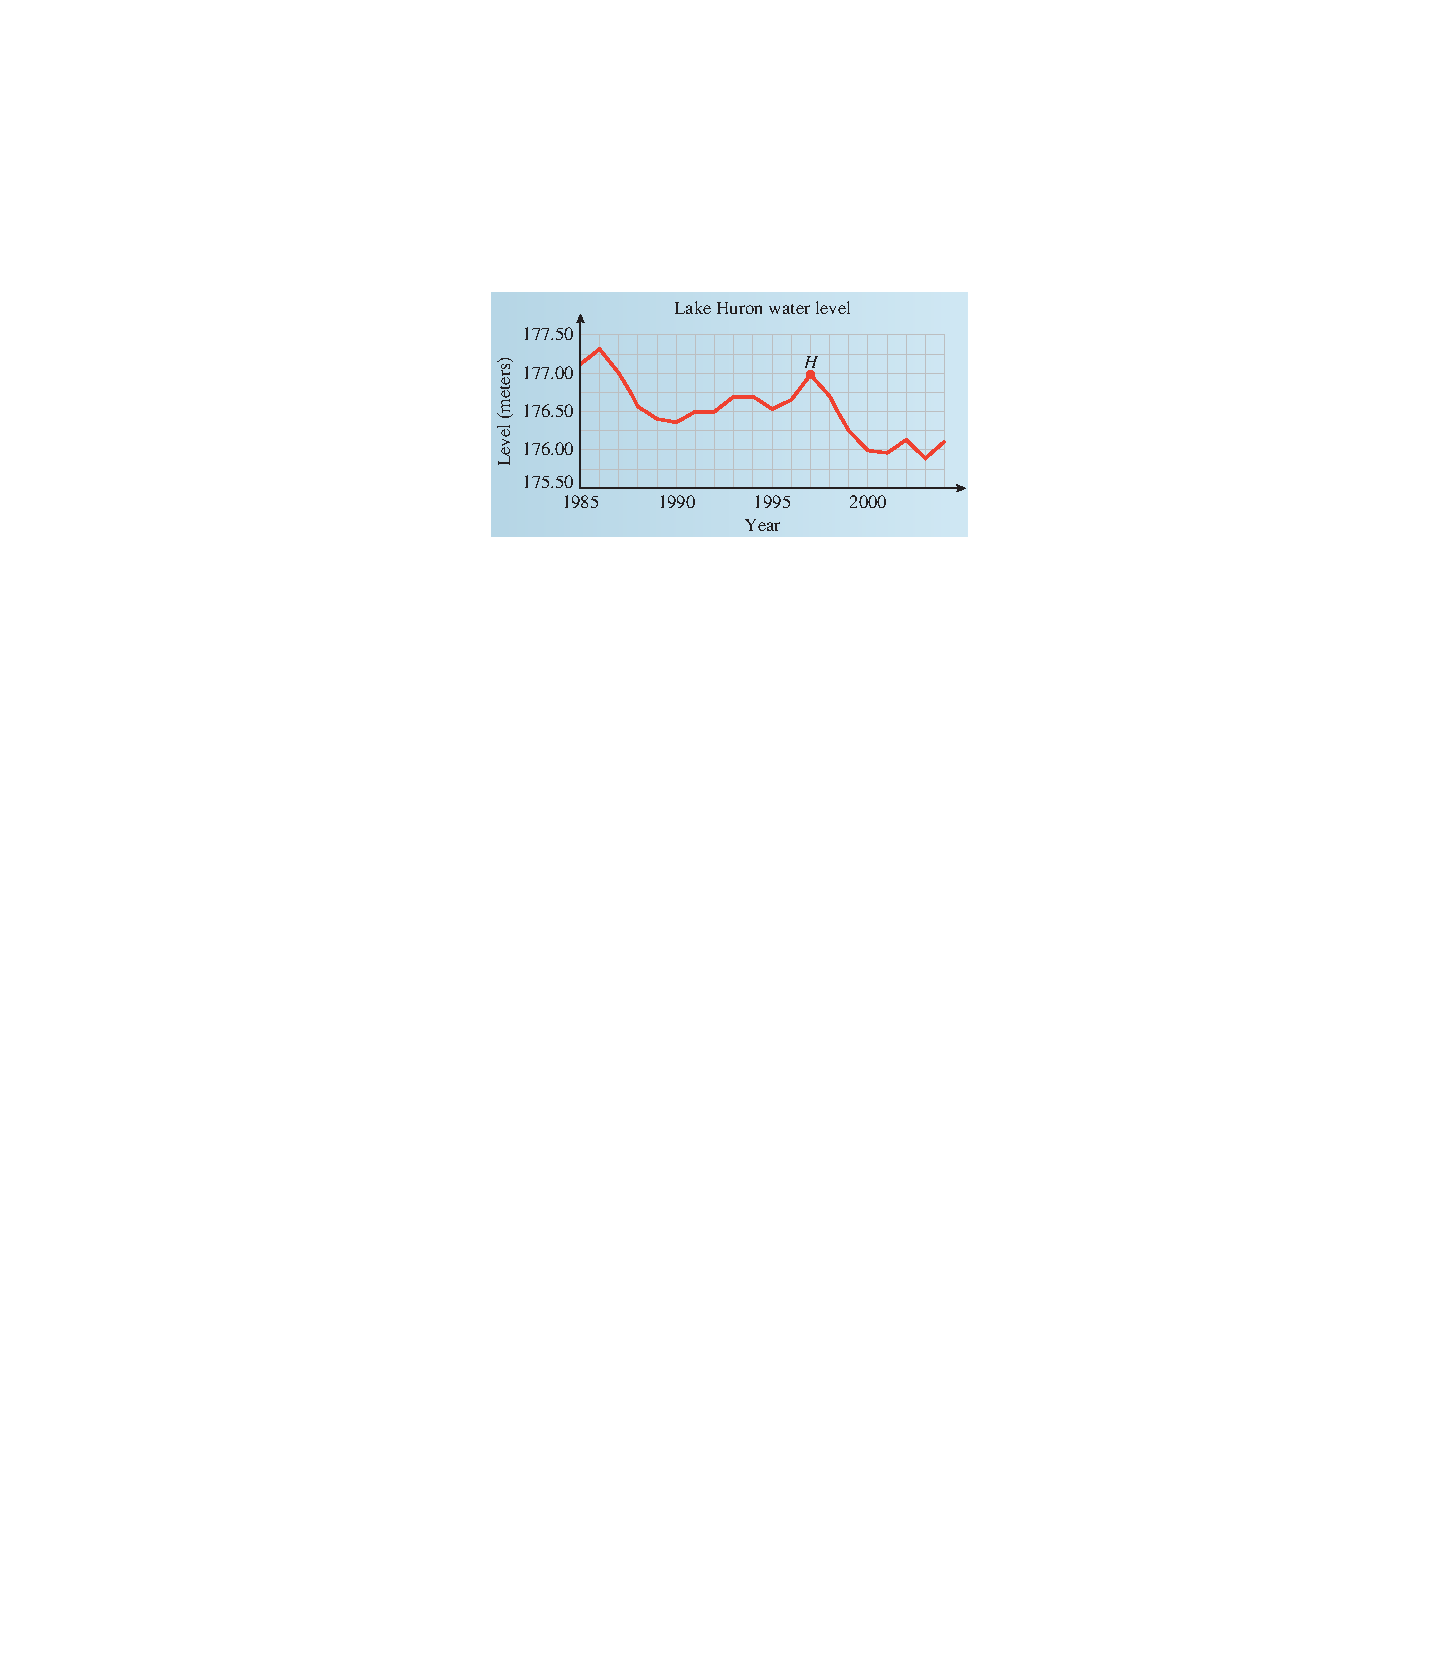
\includegraphics[width=\linewidth]{images/fig-Lake-Huron}
\end{sbspanel}%
\end{sidebyside}%
\par
%
\begin{enumerate}[label=\alph*]
\item{}The coordinates of point \(H\) on the graph are \((1997, 176.98)\). What do the coordinates tell you about the function \(L\)?%
\item{}The average water level in \(2004\) was \(176.11\) meters. Write this fact in function notation. What can you say about the graph of \(L\)?%
\end{enumerate}
%
\par\smallskip%
\noindent\textbf{\blocktitlefont Answer}.\quad{}%
\begin{enumerate}[label=\alph*]
\item{}\(L(1997) = 176.98\); the average water level was \(176.98\) meters in \(1997\).%
\item{}\(L(2004) = 176.11\). The point \((2004, 176.11)\) lies on the graph of \(L\).%
\end{enumerate}
%
\end{inlineexercisesolution}
\begin{inlineexercisesolution}{1.3.4}{}{g:exercise:idm93549583664}
Refer to the graph of the function \(g\) shown in Example~1.3.3.%
\begin{enumerate}[label=\alph*]
\item{}Find \(g(0)\).%
\item{}For what value(s) of \(t\) is \(g(t) = 0\)?%
\item{}What is the smallest, or minimum, value of \(g(t)\)? For what value of \(t\) does the function take on its minimum value?%
\item{}On what intervals is \(g\) decreasing?%
\end{enumerate}
%
\par\smallskip%
\noindent\textbf{\blocktitlefont Answer}.\quad{}%
\begin{multicols}{2}
\begin{enumerate}[label=\alph*]
\item{}\(3\)%
\item{}\(-2, 2, 4\)%
\item{}\(-3\); \(t = -4\)%
\item{}\((-5, -4)\) and \((1, 3)\)%
\end{enumerate}
\end{multicols}
%
\end{inlineexercisesolution}
\subsection*{1.3.2 Constructing the Graph of a Function}
\addcontentsline{toc}{subsection}{1.3.2 Constructing the Graph of a Function}
\begin{inlineexercisesolution}{1.3.6}{}{g:exercise:idm93549550912}
\(f(x) = x^3 - 2\)%
\begin{enumerate}[label=\alph*]
\item{}Complete the table of values and sketch a graph of the function.%
\begin{sidebyside}{1}{0}{0}{0}%
\begin{sbspanel}{1}%
{\centering%
{\tabularfont%
\begin{tabular}{AcAcAcAcAcAcAcAcA}\hrulethick
\(x\)&\(-2\)&\(-1\)&\(-\frac{1}{2}\)&\(0\)&\(\frac{1}{2}\)&\(1\)&\(2\)\tabularnewline\hrulethin
\(f(x)\)&\(\hphantom{000}\)&\(\hphantom{000}\)&\(\hphantom{000}\)&\(\hphantom{000}\)&\(\hphantom{000}\)&\(\hphantom{000}\)&\(\hphantom{000}\)\tabularnewline\hrulethin
\end{tabular}
}%
\par}
\end{sbspanel}%
\end{sidebyside}%
\item{}Use your calculator to make a table of values and graph the function.%
\end{enumerate}
%
\par\smallskip%
\noindent\textbf{\blocktitlefont Answer}.\quad{}%
\begin{enumerate}[label=\alph*]
\item{}\begin{sidebyside}{1}{0}{0.4}{0}%
\begin{sbspanel}{0.6}%
{\centering%
{\tabularfont%
\begin{tabular}{AcAcAcAcAcAcAcAcA}\hrulethick
\(x\)&\(-2\)&\(-1\)&\(-\frac{1}{2}\)&\(0\)&\(\frac{1}{2}\)&\(1\)&\(2\)\tabularnewline\hrulethin
\(f(x)\)&\(-10 \)&\(-3 \)&\(\frac{-17}{8}\)&\(-2\)&\(\frac{-15}{8} \)&\(-1\)&\(6\)\tabularnewline\hrulethin
\end{tabular}
}%
\par}
\end{sbspanel}%
\end{sidebyside}%
%
\item{}\begin{sidebyside}{1}{0}{0.75}{0}%
\begin{sbspanel}{0.2}%
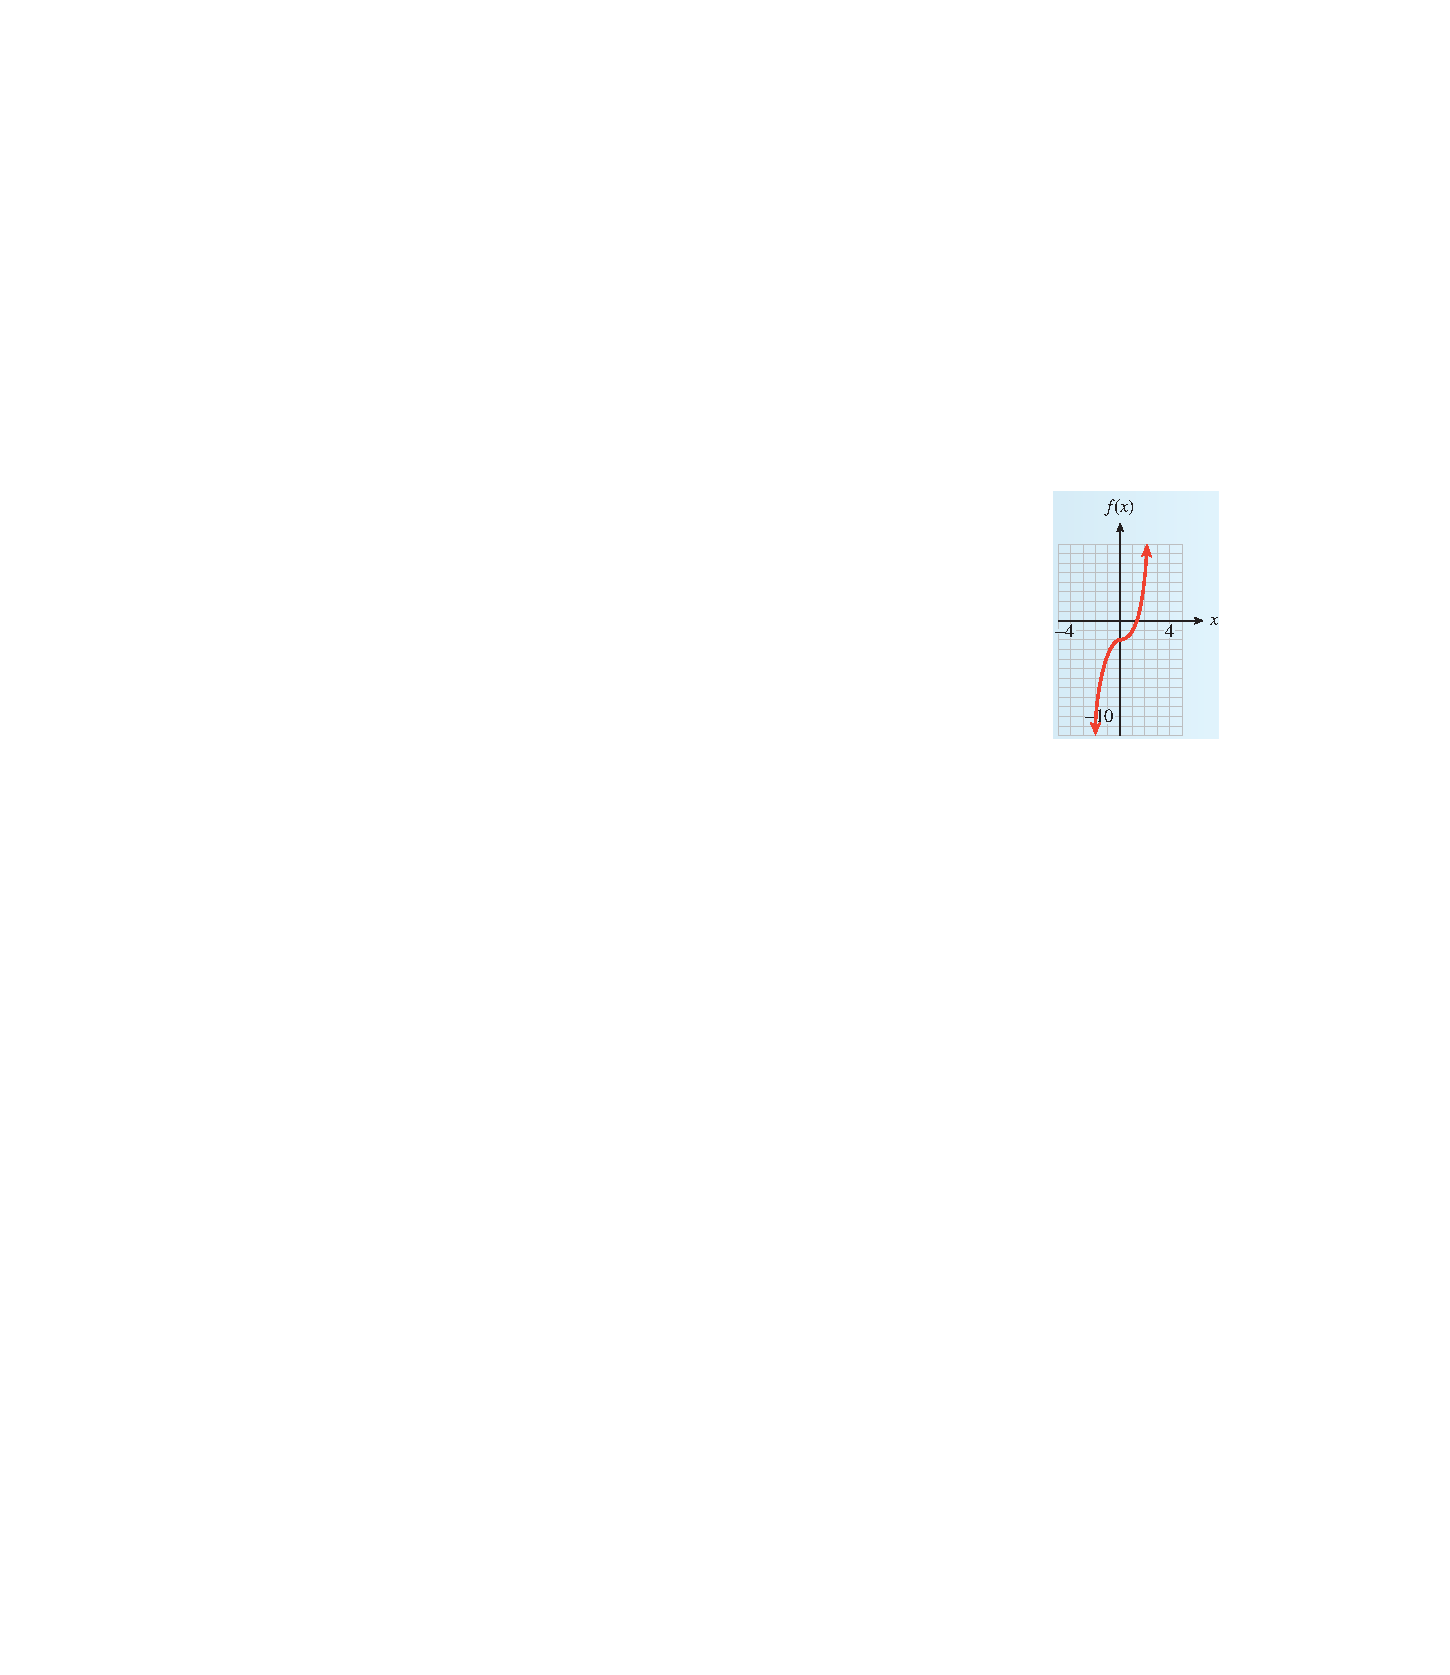
\includegraphics[width=\linewidth]{images/fig-in-ex-ans-1-3-3}
\end{sbspanel}%
\end{sidebyside}%
%
\end{enumerate}
%
\end{inlineexercisesolution}
\subsection*{1.3.3 The Vertical Line Test}
\addcontentsline{toc}{subsection}{1.3.3 The Vertical Line Test}
\begin{inlineexercisesolution}{1.3.8}{}{g:exercise:idm93549505216}
Use the vertical line test to determine which of the graphs below represent functions.%
\begin{sidebyside}{1}{0}{0}{0}%
\begin{sbspanel}{1}%
\includegraphics[width=\linewidth]{images/fig-vertical-line-test3}
\end{sbspanel}%
\end{sidebyside}%
\par\smallskip%
\noindent\textbf{\blocktitlefont Answer}.\quad{}Only (b) is a function.%
\end{inlineexercisesolution}
\subsection*{1.3.4 Graphical Solution of Equations and Inequalities}
\addcontentsline{toc}{subsection}{1.3.4 Graphical Solution of Equations and Inequalities}
\begin{inlineexercisesolution}{1.3.11}{}{g:exercise:idm93549473664}
%
\begin{enumerate}[label=\alph*]
\item{}Use the graph of \(y = 30 - 8x\) shown in the figure to solve the equation%
\begin{equation*}
30 - 8x = 50
\end{equation*}
%
\item{}Verify your solution algebraically.%
\end{enumerate}
\begin{sidebyside}{1}{0.35}{0.35}{0}%
\begin{sbspanel}{0.3}%
\includegraphics[width=\linewidth]{images/fig-graph-to-solve2}
\end{sbspanel}%
\end{sidebyside}%
\par\smallskip%
\noindent\textbf{\blocktitlefont Answer}.\quad{}\(-2.5\)%
\end{inlineexercisesolution}
\begin{inlineexercisesolution}{1.3.13}{}{g:exercise:idm93549448768}
%
\begin{enumerate}[label=\alph*]
\item{}Use the graph of \(y = 30 - 8x\) in  the previous Checkpoint to solve the inequality%
\begin{equation*}
30 - 8x \le 50
\end{equation*}
%
\item{}Solve the inequality algebraically.%
\end{enumerate}
\par\smallskip%
\noindent\textbf{\blocktitlefont Answer}.\quad{}\(x\ge -2.5\)%
\end{inlineexercisesolution}
\begin{inlineexercisesolution}{1.3.15}{}{x:exercise:exercise-graph-to-solve-quadratic}
Use the graph of \(~y = \frac{1}{2}n^2 + 2n - 10~\) shown below to solve%
\begin{equation*}
\frac{1}{2}n^2 + 2n - 10 = 6
\end{equation*}
and verify your solutions algebraically.%
\begin{sidebyside}{1}{0.35}{0.35}{0}%
\begin{sbspanel}{0.3}%
\includegraphics[width=\linewidth]{images/fig-graph-to-solve-quadratic}
\end{sbspanel}%
\end{sidebyside}%
\par\smallskip%
\noindent\textbf{\blocktitlefont Answer}.\quad{}\(-8, 4\)%
\end{inlineexercisesolution}
\begin{inlineexercisesolution}{1.3.17}{}{g:exercise:idm93549422048}
Use the graph in Checkpoint~1.3.15 to solve the inequality%
\begin{equation*}
\frac{1}{2}n^2 + 2n - 10 \lt 6
\end{equation*}
%
\par\smallskip%
\noindent\textbf{\blocktitlefont Answer}.\quad{}\((-8, 4)\)%
\end{inlineexercisesolution}
\subsection*{1.3.6 Homework 1.3}
\addcontentsline{toc}{subsection}{1.3.6 Homework 1.3}
In Problems 1\textendash{}8, use the graphs to answer the questions about the functions.%
\begin{exercisegroup}
\begin{divisionsolutioneg}{1.3.6.1}{}{g:exercise:idm93549388288}%
%
\begin{enumerate}[label=\alph*]
\item{}Find \(h(-3)\), \(h(1)\), and \(h(3)\).%
\item{}For what value(s) of \(z\) is \(h(z) = 3\)?%
\item{}Find the intercepts of the graph. List the function values given by the intercepts.%
\item{}What is the maximum value of \(h(z)\)?%
\item{}For what value(s) of \(z\) does \(h\) take on its maximum value?%
\item{}On what intervals is the function increasing? Decreasing?%
\end{enumerate}
%
\begin{sidebyside}{1}{0.325}{0.325}{0}%
\begin{sbspanel}{0.35}%
\includegraphics[width=\linewidth]{images/fig-ex-1-3-1}
\end{sbspanel}%
\end{sidebyside}%
\par\smallskip%
\noindent\textbf{\blocktitlefont Answer}.\quad{}%
\begin{enumerate}[label=\alph*]
\item{}\(\displaystyle -2, 0,5\)%
\item{}\(\displaystyle 2\)%
\item{}\(\displaystyle h(-2)=0,~h(1)=0,~h(0)=-2\)%
\item{}\(\displaystyle 5\)%
\item{}\(\displaystyle 3\)%
\item{}Increasing: \((-3,0)\) and \((1,3)\); decreasing: \((0,1)\) and \((3,5)\)%
\end{enumerate}
%
\end{divisionsolutioneg}%
\begin{divisionsolutioneg}{1.3.6.2}{}{g:exercise:idm93549373168}%
%
\begin{enumerate}[label=\alph*]
\item{}Find \(G(-3)\), \(G(-1)\), and \(G(2)\).%
\item{}For what value(s) of \(s\) is \(G(s) = 3\)?%
\item{}Find the intercepts of the graph. List the function values given by the intercepts.%
\item{}What is the minimum value of \(G(s)\)?%
\item{}For what value(s) of \(s\) does \(G\) take on its minimum value?%
\item{}On what intervals is the function increasing? Decreasing?%
\end{enumerate}
%
\begin{sidebyside}{1}{0.325}{0.325}{0}%
\begin{sbspanel}{0.35}%
\includegraphics[width=\linewidth]{images/fig-ex-1-3-2}
\end{sbspanel}%
\end{sidebyside}%
\end{divisionsolutioneg}%
\begin{divisionsolutioneg}{1.3.6.3}{}{g:exercise:idm93549363696}%
%
\begin{enumerate}[label=\alph*]
\item{}Find \(R(1)\) and \(R(3)\).%
\item{}For what value(s) of \(p\) is \(R(p)=2\)?%
\item{}Find the intercepts of the graph. List the function values given by the intercepts.%
\item{}Find the maximum and minimum values of \(R(p)\).%
\item{}For what value(s) of \(p\) does \(R\) take on its maximum and minimum values?%
\item{}On what intervals is the function increasing? Decreasing?%
\end{enumerate}
%
\begin{sidebyside}{1}{0.325}{0.325}{0}%
\begin{sbspanel}{0.35}%
\includegraphics[width=\linewidth]{images/fig-ex-1-3-3}
\end{sbspanel}%
\end{sidebyside}%
\par\smallskip%
\noindent\textbf{\blocktitlefont Answer}.\quad{}%
\begin{enumerate}[label=\alph*]
\item{}\(-1, 2\)%
\item{}\(3, -1.3\)%
\item{}\(R(-2) = 0\), \(R(2) = 0\), \(R(4) = 0\), \(R(0) = 4\)%
\item{}Max: \(4\); min: \(-5\)%
\item{}Max at \(p = 0\); min at \(p = 5\)%
\item{}Increasing: \((-3, 0)\) and \((1, 3)\); decreasing: \((0, 1)\) and \((3, 5)\)%
\end{enumerate}
%
\end{divisionsolutioneg}%
\begin{divisionsolutioneg}{1.3.6.4}{}{g:exercise:idm93549345936}%
%
\begin{enumerate}[label=\alph*]
\item{}Find \(f (-1)\) and \(f (3)\).%
\item{}For what value(s) of \(t\) is \(f(t)=5\)?%
\item{}Find the intercepts of the graph. List the function values given by the intercepts.%
\item{}Find the maximum and minimum values of \(f(t)\).%
\item{}For what value(s) of \(t\) does \(f\) take on its maximum and minimum values?%
\item{}On what intervals is the function increasing? Decreasing?%
\end{enumerate}
%
\begin{sidebyside}{1}{0.325}{0.325}{0}%
\begin{sbspanel}{0.35}%
\includegraphics[width=\linewidth]{images/fig-ex-1-3-4}
\end{sbspanel}%
\end{sidebyside}%
\end{divisionsolutioneg}%
\begin{divisionsolutioneg}{1.3.6.5}{}{g:exercise:idm93549336848}%
%
\begin{enumerate}[label=\alph*]
\item{}Find \(S(0)\), \(S\left(\dfrac{1}{6}\right)\), and \(S(-1)\).%
\item{}Estimate the value of \(S\left(\dfrac{1}{3}\right)\) from the graph.%
\item{}For what value(s) of \(x\) is \(S(x) = -\dfrac{1}{2}\)?%
\item{}Find the maximum and minimum values of \(S(x)\).%
\item{}For what value(s) of \(x\) does \(S\) take on its maximum and minimum values?%
\end{enumerate}
%
\begin{sidebyside}{1}{0.25}{0.25}{0}%
\begin{sbspanel}{0.5}%
\includegraphics[width=\linewidth]{images/fig-ex-1-3-5}
\end{sbspanel}%
\end{sidebyside}%
\par\smallskip%
\noindent\textbf{\blocktitlefont Answer}.\quad{}%
\begin{enumerate}[label=\alph*]
\item{}\(0, \dfrac{1}{2}, 0\)%
\item{}\(0.9\)%
\item{}\(\dfrac{-5}{6}\), \(\dfrac{-1}{6}\), \(\dfrac{7}{6}\), \(\dfrac{11}{6}\)%
\item{}Max: \(1\); min: \(-1\)%
\item{}Max at \(x=-1.5, 0.5\); min at \(x=-0.5, 1.5\)%
\end{enumerate}
%
\end{divisionsolutioneg}%
\begin{divisionsolutioneg}{1.3.6.6}{}{g:exercise:idm93549320928}%
%
\begin{enumerate}[label=\alph*]
\item{}Find \(C(0)\), \(C\left(-\dfrac{1}{3}\right)\), and \(C(1)\).%
\item{}Estimate the value of \(C\left(\dfrac{1}{6}\right)\) from the graph.%
\item{}For what value(s) of \(x\) is \(C(x) = \dfrac{1}{2}\)?%
\item{}Find the maximum and minimum values of \(C(x)\).%
\item{}For what value(s) of \(x\) does \(C\) take on its maximum and minimum values?%
\end{enumerate}
%
\begin{sidebyside}{1}{0.25}{0.25}{0}%
\begin{sbspanel}{0.5}%
\includegraphics[width=\linewidth]{images/fig-ex-1-3-6}
\end{sbspanel}%
\end{sidebyside}%
\end{divisionsolutioneg}%
\begin{divisionsolutioneg}{1.3.6.7}{}{g:exercise:idm93549311616}%
%
\begin{enumerate}[label=\alph*]
\item{}Find \(F(-3)\), \(F(-2)\), and \(F(2)\).%
\item{}For what value(s) of \(s\) is \(F(s) = -1\)?%
\item{}Find the maximum and minimum values of \(F(s)\).%
\item{}For what value(s) of \(s\) does \(F\) take on its maximum and minimum values?%
\end{enumerate}
%
\begin{sidebyside}{1}{0.3}{0.3}{0}%
\begin{sbspanel}{0.4}%
\includegraphics[width=\linewidth]{images/fig-ex-1-3-7}
\end{sbspanel}%
\end{sidebyside}%
\par\smallskip%
\noindent\textbf{\blocktitlefont Answer}.\quad{}%
\begin{enumerate}[label=\alph*]
\item{}\(2, 2, 1\)%
\item{}\(-6 \le s \lt -4~\) or \(~0\le s\lt 2\)%
\item{}Max: \(2\); min: \(-1\)%
\item{}Max for \(-3\le s\lt -1~\) or \(~3\le s\lt 5\); min for \(-6\le s\lt -4~\) or \(~0\le s\lt 2\)%
\end{enumerate}
%
\end{divisionsolutioneg}%
\begin{divisionsolutioneg}{1.3.6.8}{}{g:exercise:idm93549297504}%
%
\begin{enumerate}[label=\alph*]
\item{}Find \(P(-3)\), \(P(-2)\), and \(P(1)\).%
\item{}For what value(s) of \(n\) is \(P(n) = 0\)?%
\item{}Find the maximum and minimum values of \(P(n)\).%
\item{}For what value(s) of \(n\) does \(P\) take on its maximum and minimum values?%
\end{enumerate}
%
\begin{sidebyside}{1}{0.3}{0.3}{0}%
\begin{sbspanel}{0.4}%
\includegraphics[width=\linewidth]{images/fig-ex-1-3-8}
\end{sbspanel}%
\end{sidebyside}%
\end{divisionsolutioneg}%
\end{exercisegroup}
\par\medskip\noindent
Which of the graphs in Problems 9 and 10 represent functions?%
\begin{exercisegroup}
\begin{divisionsolutioneg}{1.3.6.9}{}{g:exercise:idm93549288384}%
\begin{sidebyside}{1}{0}{0}{0}%
\begin{sbspanel}{1}%
\includegraphics[width=\linewidth]{images/fig-ex-1-3-9}
\end{sbspanel}%
\end{sidebyside}%
\par\smallskip%
\noindent\textbf{\blocktitlefont Answer}.\quad{}(a) and (d)%
\end{divisionsolutioneg}%
\begin{divisionsolutioneg}{1.3.6.10}{}{g:exercise:idm93549286272}%
\begin{sidebyside}{1}{0}{0}{0}%
\begin{sbspanel}{1}%
\includegraphics[width=\linewidth]{images/fig-ex-1-3-10}
\end{sbspanel}%
\end{sidebyside}%
\end{divisionsolutioneg}%
\end{exercisegroup}
\par\medskip\noindent
In Problems 11\textendash{}16,%
\begin{enumerate}[label=\alph*]
\item{}Make a table of values and sketch a graph of the function by plotting points. (Use the suggested \(x\)-values.)%
\item{}Use your calculator to graph the function.%
\end{enumerate}
Compare the calculator's graph with your sketch.%
\begin{exercisegroupcol}{2}
\begin{divisionsolutionegcol}{1.3.6.11}{}{g:exercise:idm93549281040}%
\(g(x) = x^3 + 4\); \(\hphantom{00000}x = -2, -1, \ldots , 2\)%
\par\smallskip%
\noindent\textbf{\blocktitlefont Answer}.\quad{}\begin{sidebyside}{1}{0.225}{0.225}{0}%
\begin{sbspanel}{0.55}%
\includegraphics[width=\linewidth]{images/fig-ans-1-3-11}
\end{sbspanel}%
\end{sidebyside}%
\end{divisionsolutionegcol}%
\begin{divisionsolutionegcol}{1.3.6.12}{}{g:exercise:idm93549278112}%
\(h(x) = 2 +\sqrt{x}\); \(\hphantom{00000}x = 0,1, \ldots , 9\)%
\end{divisionsolutionegcol}%
\begin{divisionsolutionegcol}{1.3.6.13}{}{g:exercise:idm93549276464}%
\(G(x) =\sqrt{4 - x}\); \(\hphantom{00000}x = -5, -4, \ldots , 4\)%
\par\smallskip%
\noindent\textbf{\blocktitlefont Answer}.\quad{}\begin{sidebyside}{1}{0.2}{0.2}{0}%
\begin{sbspanel}{0.6}%
\includegraphics[width=\linewidth]{images/fig-ans-1-3-13}
\end{sbspanel}%
\end{sidebyside}%
\end{divisionsolutionegcol}%
\begin{divisionsolutionegcol}{1.3.6.14}{}{g:exercise:idm93549273520}%
\(F(x) = \sqrt{x-1}\); \(\hphantom{00000}x = 1,2, \ldots , 10\)%
\end{divisionsolutionegcol}%
\begin{divisionsolutionegcol}{1.3.6.15}{}{g:exercise:idm93549271872}%
\(v(x) = 1 + 6x - x^3\); \(\hphantom{00000}x = -3, -2, \ldots , 3\)%
\par\smallskip%
\noindent\textbf{\blocktitlefont Answer}.\quad{}\begin{sidebyside}{1}{0.225}{0.225}{0}%
\begin{sbspanel}{0.55}%
\includegraphics[width=\linewidth]{images/fig-ans-1-3-15}
\end{sbspanel}%
\end{sidebyside}%
\end{divisionsolutionegcol}%
\begin{divisionsolutionegcol}{1.3.6.16}{}{g:exercise:idm93549268928}%
\(w(x) = x^3 - 8x\); \(\hphantom{00000}x = -4, -3, \ldots , 4\)%
\end{divisionsolutionegcol}%
\end{exercisegroupcol}
\par\medskip\noindent
\begin{divisionsolution}{1.3.6.17}{}{g:exercise:idm93549267152}%
The graph shows the speed of sound in the ocean as a function of depth, \(S = f (d)\). The speed of sound is affected both by increasing water pressure and by dropping temperature. (Source: Scientific American)%
\begin{sidebyside}{1}{0.3}{0.3}{0}%
\begin{sbspanel}{0.4}%
\includegraphics[width=\linewidth]{images/fig-ex-1-3-17}
\end{sbspanel}%
\end{sidebyside}%
\par
%
\begin{enumerate}[label=\alph*]
\item{}Evaluate \(f (1000)\) and explain its meaning.%
\item{}Solve \(f (d) = 1500\) and explain its meaning.%
\item{}At what depth is the speed of sound the slowest, and what is the speed? Write your answer with function notation.%
\item{}Describe the behavior of \(f (d)\) as \(d\) increases.%
\end{enumerate}
%
\par\smallskip%
\noindent\textbf{\blocktitlefont Answer}.\quad{}%
\begin{enumerate}[label=\alph*]
\item{}\(f (1000) = 1495\): The speed of sound at a depth of \(1000\) meters is approximately \(1495\) meters per second.%
\item{}\(d = 570\) or \(d = 1070\): The speed of sound is \(1500\) meters per second at both a depth of \(570\) meters and a depth of \(1070\) meters.%
\item{}The slowest speed occurs at a depth of about \(810\) meters and the speed is about \(1487\) meters per second, so \(f (810) = 1487\).%
\item{}\(f\) increases from about \(1533\) to \(1541\) in the first \(110\) meters of depth, then drops to about \(1487\) at \(810\) meters, then rises again, passing \(1553\) at a depth of about \(1600\) meters.%
\end{enumerate}
%
\end{divisionsolution}%
\begin{divisionsolution}{1.3.6.18}{}{g:exercise:idm93549249200}%
The graph shows the water level in Lake Superior as a function of time, \(L = f (t)\). (Source: The Canadian Hydrographic Service)%
\begin{sidebyside}{1}{0.2}{0.2}{0}%
\begin{sbspanel}{0.6}%
\includegraphics[width=\linewidth]{images/fig-ex-1-3-18}
\end{sbspanel}%
\end{sidebyside}%
\par
%
\begin{enumerate}[label=\alph*]
\item{}Evaluate \(f (1997)\) and explain its meaning.%
\item{}Solve \(f (t) = 183.5\) and explain its meaning.%
\item{}In which two years did Lake Superior reach its highest levels, and what were those levels? Write your answers with function notation.%
\item{}Over which two-year period did the water level drop the most?%
\end{enumerate}
%
\end{divisionsolution}%
\begin{divisionsolution}{1.3.6.19}{}{g:exercise:idm93549242672}%
The graph shows the federal debt as a percentage of the gross domestic product (GDP), as a function of time, \(D = f (t)\). (Source: Office of Management and Budget)%
\begin{sidebyside}{1}{0.3}{0.3}{0}%
\begin{sbspanel}{0.4}%
\includegraphics[width=\linewidth]{images/fig-ex-1-3-19}
\end{sbspanel}%
\end{sidebyside}%
\par
%
\begin{enumerate}[label=\alph*]
\item{}Evaluate \(f (1985)\) and explain its meaning.%
\item{}Solve \(f (t) = 70\) and explain its meaning.%
\item{}When did the federal debt reach its highest level since 1960, and what was that level? Write your answer with function notation.%
\item{}What is the longest time interval over which the federal debt was decreasing?%
\end{enumerate}
%
\par\smallskip%
\noindent\textbf{\blocktitlefont Answer}.\quad{}%
\begin{enumerate}[label=\alph*]
\item{}\(f(1985)=41\): The federal debt in \(1985\) was about \(41\%\) of the gross domestic product.%
\item{}\(t = 1942\) or \(t = 1955\): The federal debt was \(70\%\) of the gross domestic product in \(1942\) and \(1955\).%
\item{}In about \(1997\), the debt was about \(67\%\) of the gross domestic product, so \(f (1997)\approx 67.3\).%
\item{}The percentage basically dropped from 1946 to 1973, but there were small rises around 1950, 1954, 1958, and 1968, so the longest time interval was from 1958 to 1967.%
\end{enumerate}
%
\end{divisionsolution}%
\begin{divisionsolution}{1.3.6.20}{}{g:exercise:idm93549228288}%
The graph shows the elevation of the Los Angeles Marathon course as a function of the distance into the race, \(a = f (t)\). (Source: Los Angeles Times, March 3, 2005)%
\begin{sidebyside}{1}{0.15}{0.15}{0}%
\begin{sbspanel}{0.7}%
\includegraphics[width=\linewidth]{images/fig-ex-1-3-20}
\end{sbspanel}%
\end{sidebyside}%
\par
%
\begin{enumerate}[label=\alph*]
\item{}Evaluate \(f (5)\) and explain its meaning.%
\item{}Solve \(f (d) = 200\) and explain its meaning.%
\item{}When does the marathon course reach its lowest elevation, and what is that elevation? Write your answer with function notation.%
\item{}Give three intervals over which the elevation is increasing.%
\end{enumerate}
%
\end{divisionsolution}%
\begin{divisionsolution}{1.3.6.21}{}{g:exercise:idm93549221744}%
The figure shows a graph of \(y = -2x + 6\).%
\begin{sidebyside}{1}{0.325}{0.325}{0}%
\begin{sbspanel}{0.35}%
\includegraphics[width=\linewidth]{images/fig-ex-1-3-21}
\end{sbspanel}%
\end{sidebyside}%
\par
%
\begin{enumerate}[label=\alph*]
\item{}Use the graph to find all values of \(x\) for which%
\begin{enumerate}[label=\Roman*]
\item{}\(y=12\)%
\item{}\(y\gt 12\)%
\item{}\(y\lt 12\)%
\end{enumerate}
%
\item{}Use the graph to solve%
\begin{enumerate}[label=\Roman*]
\item{}\(-2x + 6=12\)%
\item{}\(-2x + 6\gt 12\)%
\item{}\(-2x + 6\lt 12\)%
\end{enumerate}
%
\item{}Explain why your answers to parts (a) and (b) are the same.%
\end{enumerate}
%
\par\smallskip%
\noindent\textbf{\blocktitlefont Answer}.\quad{}%
\begin{enumerate}[label=\alph*]
\item{}%
\begin{enumerate}[label=\roman*]
\item{}\(x = -3\)%
\item{}\(x\lt -3\)%
\item{}\(x\gt -3\)%
\end{enumerate}
%
\item{}%
\begin{enumerate}[label=\Roman*]
\item{}\(x = -3\)%
\item{}\(x\lt -3\)%
\item{}\(x\gt -3\)%
\end{enumerate}
%
\item{}On the graph of \(y=-2x + 6\), a value of \(y\) is the same as a value of \(-2x + 6\), so parts (a) and (b) are asking for the same \(x\)'s.%
\end{enumerate}
%
\end{divisionsolution}%
\begin{divisionsolution}{1.3.6.22}{}{g:exercise:idm93549201824}%
The figure shows a graph of \(y =\dfrac{-x}{3} - 6\).%
\begin{sidebyside}{1}{0.3}{0.3}{0}%
\begin{sbspanel}{0.4}%
\includegraphics[width=\linewidth]{images/fig-ex-1-3-22}
\end{sbspanel}%
\end{sidebyside}%
\par
%
\begin{enumerate}[label=\alph*]
\item{}Use the graph to find all values of \(x\) for which%
\begin{enumerate}[label=\roman*]
\item{}\(y=-4\)%
\item{}\(y\gt -4\)%
\item{}\(y\lt -4\)%
\end{enumerate}
%
\item{}Use the graph to solve%
\begin{enumerate}[label=\roman*]
\item{}\(\dfrac{-x}{3} - 6=-4\)%
\item{}\(\dfrac{-x}{3} - 6\gt -4\)%
\item{}\(\dfrac{-x}{3} - 6\lt -4\)%
\end{enumerate}
%
\item{}Explain why your answers to parts (a) and (b) are the same.%
\end{enumerate}
%
\end{divisionsolution}%
In Problems 23 and 24, use the graph to solve the equation or inequality, and then solve algebraically. (To review solving linear inequalities algebraically, see Algebra Skills Refresher~A.2.)%
\begin{exercisegroup}
\begin{divisionsolutioneg}{1.3.6.23}{}{g:exercise:idm93549189280}%
The figure shows the graph of \(y = 1.4x - 0.64\). Solve the following:%
\begin{sidebyside}{1}{0.35}{0.35}{0}%
\begin{sbspanel}{0.3}%
\includegraphics[width=\linewidth]{images/fig-ex-1-3-23}
\end{sbspanel}%
\end{sidebyside}%
\par
%
\begin{enumerate}[label=\alph*]
\item{}\(1.4x - 0.64 = 0.2\)%
\item{}\(-1.2 = 1.4x - 0.64\)%
\item{}\(1.4x - 0.64\gt 0.2\)%
\item{}\(-1.2\gt 1.4x - 0.64\)%
\end{enumerate}
%
\par\smallskip%
\noindent\textbf{\blocktitlefont Answer}.\quad{}%
\begin{enumerate}[label=\alph*]
\item{}\(x = 0.6\)%
\item{}\(x=-0.4\)%
\item{}\(x\gt 0.6\)%
\item{}\(x\lt -0.4\)%
\end{enumerate}
%
\end{divisionsolutioneg}%
\begin{divisionsolutioneg}{1.3.6.24}{}{g:exercise:idm93549179632}%
The figure shows the graph of \(y = -2.4x + 2.32\). Solve the following:%
\begin{sidebyside}{1}{0.325}{0.325}{0}%
\begin{sbspanel}{0.35}%
\includegraphics[width=\linewidth]{images/fig-ex-1-3-24}
\end{sbspanel}%
\end{sidebyside}%
\par
%
\begin{enumerate}[label=\alph*]
\item{}\(1.6 = -2.4x + 2.32\)%
\item{}\(-2.4x + 2.32 = 0.4\)%
\item{}\(-2.4x + 2.32\ge 1.6\)%
\item{}\(0.4\ge -2.4x + 2.32\)%
\end{enumerate}
%
\end{divisionsolutioneg}%
\end{exercisegroup}
\par\medskip\noindent
For Problems 25\textendash{}30, use the graphs to estimate solutions to the equations and inequalities.%
\begin{exercisegroup}
\begin{divisionsolutioneg}{1.3.6.25}{}{g:exercise:idm93549172464}%
The figure shows the graph of \(g(x) = \dfrac{12}{2 + x^2}\).%
\begin{sidebyside}{1}{0.325}{0.325}{0}%
\begin{sbspanel}{0.35}%
\includegraphics[width=\linewidth]{images/fig-ex-1-3-25}
\end{sbspanel}%
\end{sidebyside}%
\par
%
\begin{enumerate}[label=\alph*]
\item{}Solve \(\dfrac{12}{2 + x^2} = 4\)%
\item{}Solve \(1\le \dfrac{12}{2 + x^2} \le 2\)%
\end{enumerate}
%
\par\smallskip%
\noindent\textbf{\blocktitlefont Answer}.\quad{}%
\begin{enumerate}[label=\alph*]
\item{}\(x=-1\)  or \(x = 1\)%
\item{}Approximately \(-3\le x\le -2\)  or \(2\le x\le 3\)%
\end{enumerate}
%
\end{divisionsolutioneg}%
\begin{divisionsolutioneg}{1.3.6.26}{}{g:exercise:idm93549164192}%
The figure shows the graph of \(f(x) = \dfrac{30\sqrt{x}}{1 + x}\).%
\begin{sidebyside}{1}{0.3}{0.3}{0}%
\begin{sbspanel}{0.4}%
\includegraphics[width=\linewidth]{images/fig-ex-1-3-26}
\end{sbspanel}%
\end{sidebyside}%
\par
%
\begin{enumerate}[label=\alph*]
\item{}Solve \(\dfrac{30\sqrt{x}}{1 + x} = 15\)%
\item{}Solve \(\dfrac{30\sqrt{x}}{1 + x} \lt 12\)%
\end{enumerate}
%
\end{divisionsolutioneg}%
\begin{divisionsolutioneg}{1.3.6.27}{}{g:exercise:idm93549159152}%
The figure shows a graph of \(B = \dfrac{1}{3}p^3 - 3p + 2\).%
\begin{sidebyside}{1}{0.3}{0.3}{0}%
\begin{sbspanel}{0.4}%
\includegraphics[width=\linewidth]{images/fig-ex-1-3-27}
\end{sbspanel}%
\end{sidebyside}%
\par
%
\begin{enumerate}[label=\alph*]
\item{}Solve \(\dfrac{1}{3}p^3 - 3p + 2 = 6\)%
\item{}Solve \(\dfrac{1}{3}p^3 - 3p + 2=5\)%
\item{}Solve \(\dfrac{1}{3}p^3 - 3p + 2\lt 1\)%
\item{}What range of values does \(B\) have for \(p\) between \(-2.5\) and \(0.5\)?%
\item{}For what values of \(p\) is \(B\) increasing?%
\end{enumerate}
%
\par\smallskip%
\noindent\textbf{\blocktitlefont Answer}.\quad{}%
\begin{enumerate}[label=\alph*]
\item{}\(3.5\)%
\item{}\(-2.2, -1.2, 3.4\)%
\item{}\(p\lt -3.1\) or \(0.3\lt p\lt 2.8\)%
\item{}\(0.5\lt B\lt 5.5\)%
\item{}\(p\lt -1.7\) or \(p\gt 1.7\)%
\end{enumerate}
%
\end{divisionsolutioneg}%
\begin{divisionsolutioneg}{1.3.6.28}{}{g:exercise:idm93549144464}%
The figure shows a graph of \(H = t^3 - 4t^2 - 4t + 12\).%
\begin{sidebyside}{1}{0.325}{0.325}{0}%
\begin{sbspanel}{0.35}%
\includegraphics[width=\linewidth]{images/fig-ex-1-3-28}
\end{sbspanel}%
\end{sidebyside}%
\par
%
\begin{enumerate}[label=\alph*]
\item{}Solve \(t^3 - 4t^2 - 4t + 12 = -4\)%
\item{}Solve \(t^3 - 4t^2 - 4t + 12=16\)%
\item{}Solve \(t^3 - 4t^2 - 4t + 12\gt 6\)%
\item{}Estimate the horizontal and vertical intercepts of the graph.%
\item{}For what values of \(t\) is \(H\) increasing?%
\end{enumerate}
%
\end{divisionsolutioneg}%
\begin{divisionsolutioneg}{1.3.6.29}{}{g:exercise:idm93549136592}%
The figure shows a graph of \(M = g(q)\).%
\begin{sidebyside}{1}{0.3}{0.3}{0}%
\begin{sbspanel}{0.4}%
\includegraphics[width=\linewidth]{images/fig-ex-1-3-29}
\end{sbspanel}%
\end{sidebyside}%
\par
%
\begin{enumerate}[label=\alph*]
\item{}Find all values of \(q\) for which%
\begin{enumerate}[label=\Roman*]
\item{}\(g(q) = 0\)%
\item{}\(g(q) = 16\)%
\item{}\(g(q)\lt 6\)%
\end{enumerate}
%
\item{}For what values of \(q\) is \(g(q)\) increasing?%
\end{enumerate}
%
\par\smallskip%
\noindent\textbf{\blocktitlefont Answer}.\quad{}%
\begin{enumerate}[label=\alph*]
\item{}%
\begin{enumerate}[label=\roman*]
\item{}\(-2, 2\)%
\item{}\(-2.8, 0, 2.8\)%
\item{}\(-2.5\lt q\lt-1.25\) or \(1.25\lt q\lt 2.5\)%
\end{enumerate}
%
\item{}\(-2 \lt q\lt 0\)  or \(q\gt 2\)%
\end{enumerate}
%
\end{divisionsolutioneg}%
\begin{divisionsolutioneg}{1.3.6.30}{}{g:exercise:idm93549122656}%
The figure shows a graph of \(P = f (t)\).%
\begin{sidebyside}{1}{0.35}{0.35}{0}%
\begin{sbspanel}{0.3}%
\includegraphics[width=\linewidth]{images/fig-ex-1-3-30}
\end{sbspanel}%
\end{sidebyside}%
\par
%
\begin{enumerate}[label=\alph*]
\item{}Find all values of \(t\) for which%
\begin{enumerate}[label=\Roman*]
\item{}\(f (t) = 3\)%
\item{}\(f (t)\gt 4.5\)%
\item{}\(2\le f (t)\le 4\)%
\end{enumerate}
%
\item{}For what values of \(t\) is \(f (t)\) decreasing?%
\end{enumerate}
%
\end{divisionsolutioneg}%
\end{exercisegroup}
\par\medskip\noindent
\begin{divisionsolution}{1.3.6.31}{}{g:exercise:idm93549114208}%
%
\begin{enumerate}[label=\alph*]
\item{}Delbert reads the following values from the graph of a function:%
\begin{equation*}
f (-3) = 5, ~f (-1) = 2, ~f (1) = 0,
\end{equation*}
%
\begin{equation*}
f (-1) = -4, ~f (-3) = -2
\end{equation*}
Can his readings be correct? Explain why or why not.%
\item{}Francine reads the following values from the graph of a function:%
\begin{equation*}
g(-2) = 6, ~g(0) = 0, ~g(2) = 6,
\end{equation*}
%
\begin{equation*}
g(4) = 0, ~g(6) = 6
\end{equation*}
Can her readings be correct? Explain why or why not.%
\end{enumerate}
%
\par\smallskip%
\noindent\textbf{\blocktitlefont Answer}.\quad{}%
\begin{enumerate}[label=\alph*]
\item{}He has an error: \(f(-3)\) cannot have both the value \(5\) and also the value \(-2\), and \(f(-1)\) cannot have both values \(2\) and \(-4\).%
\item{}Her readings are possible for a function: each input has only one output.%
\end{enumerate}
%
\end{divisionsolution}%
\begin{divisionsolution}{1.3.6.32}{}{g:exercise:idm93549105248}%
%
\begin{enumerate}[label=\alph*]
\item{}Sketch the graph of a function that has the following values:%
\begin{equation*}
F(-2) = 3, ~F(-1) = 3, ~F(0) = 3,
\end{equation*}
%
\begin{equation*}
F(1) = 3, ~F(2) = 3
\end{equation*}
%
\item{}Sketch the graph of a function that has the following values:%
\begin{equation*}
G(-2) = 1, ~G(-1) = 0, ~G(0) = -1,
\end{equation*}
%
\begin{equation*}
G(1) = 0, ~G(2) = 1
\end{equation*}
%
\end{enumerate}
%
\end{divisionsolution}%
For Problems 33\textendash{}36, graph each function in the friendly window%
\begin{align*}
\text{Xmin} \amp = -9.4 \amp\amp \text{Xmax} = 9.4\\
\text{Ymin} \amp = -10 \amp\amp \text{Ymax} = 10
\end{align*}
Then answer the questions about the graph. (See Appendix~B  for an explanation of friendly windows.)%
\begin{exercisegroup}
\begin{divisionsolutioneg}{1.3.6.33}{}{g:exercise:idm93549097728}%
\(g(x) =\sqrt{36 - x^2}\)%
\begin{enumerate}[label=\alph*]
\item{}Complete the table. (Round values to tenths.)%
\begin{sidebyside}{1}{0}{0}{0}%
\begin{sbspanel}{1}%
{\centering%
{\tabularfont%
\begin{tabular}{AcAcAcAcAcA}\hrulethick
\(x\)&\(-4\)&\(-2\)&\(3\)&\(5\)\tabularnewline\hrulethin
\(g(x)\)&\(\hphantom{000}\)&\(\hphantom{000}\)&\(\hphantom{000}\)&\(\hphantom{000}\)\tabularnewline\hrulethin
\end{tabular}
}%
\par}
\end{sbspanel}%
\end{sidebyside}%
\item{}Find all points on the graph for which \(g(x) = 3.6\).%
\end{enumerate}
%
\par\smallskip%
\noindent\textbf{\blocktitlefont Answer}.\quad{}%
\begin{enumerate}[label=\alph*]
\item{}\begin{sidebyside}{1}{0}{0.6}{0}%
\begin{sbspanel}{0.4}%
{\centering%
{\tabularfont%
\begin{tabular}{AcAcAcAcAcA}\hrulethick
\(x\)&\(-4\)&\(-2\)&\(3\)&\(5\)\tabularnewline\hrulethin
\(g(x)\)&\(4.5\)&\(5.7\)&\(5.2\)&\(3.3\)\tabularnewline\hrulethin
\end{tabular}
}%
\par}
\end{sbspanel}%
\end{sidebyside}%
%
\item{}\(-4.8, 4.8\)%
\end{enumerate}
%
\end{divisionsolutioneg}%
\begin{divisionsolutioneg}{1.3.6.34}{}{g:exercise:idm93549076032}%
\(g(x) =\sqrt{x^2}-6\)%
\begin{enumerate}[label=(\alph*)]
\item{}Complete the table. (Round values to tenths.)%
\begin{sidebyside}{1}{0}{0}{0}%
\begin{sbspanel}{1}%
{\centering%
{\tabularfont%
\begin{tabular}{AcAcAcAcAcA}\hrulethick
\(x\)&\(-8\)&\(-2\)&\(3\)&\(6\)\tabularnewline\hrulethin
\(f(x)\)&\(\hphantom{000}\)&\(\hphantom{000}\)&\(\hphantom{000}\)&\(\hphantom{000}\)\tabularnewline\hrulethin
\end{tabular}
}%
\par}
\end{sbspanel}%
\end{sidebyside}%
\item{}Find all points on the graph for which \(f(x) = -2\).%
\end{enumerate}
%
\end{divisionsolutioneg}%
\begin{divisionsolutioneg}{1.3.6.35}{}{g:exercise:idm93549064928}%
\(F(x) = 0.5x^3 - 4x\)%
\begin{enumerate}[label=\alph*]
\item{}Estimate the coordinates of the turning points of the graph, that is, where the graph changes from increasing to decreasing or vice versa.%
\item{}Write an equation of the form \(F(a) = b\) for each turning point.%
\end{enumerate}
%
\par\smallskip%
\noindent\textbf{\blocktitlefont Answer}.\quad{}%
\begin{enumerate}[label=\alph*]
\item{}\((-1.6, 4.352), (1.6, -4.352)\)%
\item{}\(F(-1.6) = 4.352\); \(F(1.6) = -4.352\)%
\end{enumerate}
%
\end{divisionsolutioneg}%
\begin{divisionsolutioneg}{1.3.6.36}{}{g:exercise:idm93549059232}%
\(G(x) = 2 + 4x - x^3\)%
\begin{enumerate}[label=\alph*]
\item{}Estimate the coordinates of the turning points of the graph, that is, where the graph changes from increasing to decreasing or vice versa.%
\item{}Write an equation of the form \(G(a) = b\) for each turning point.%
\end{enumerate}
%
\end{divisionsolutioneg}%
\end{exercisegroup}
\par\medskip\noindent
For Problems 37\textendash{}40, graph the function%
\begin{enumerate}[label=\alph*]
\item{}First using the standard window.%
\item{}Then using the suggested window. Explain how the window alters the appearance of the graph in each case.%
\end{enumerate}
%
\begin{exercisegroupcol}{2}
\begin{divisionsolutionegcol}{1.3.6.37}{}{g:exercise:idm93549053072}%
\(h(x) = \dfrac{1}{x^2 + 10}\)%
\begin{align*}
{\text{Xmin}} \amp = -5 \amp\amp {\text{Xmax}} = 5\\
{\text{Ymin}} \amp = 0 \amp\amp {\text{Ymax}} = 0.5
\end{align*}
%
\par\smallskip%
\noindent\textbf{\blocktitlefont Answer}.\quad{}%
\begin{enumerate}[label=\alph*]
\item{}\begin{sidebyside}{1}{0}{0.4}{0}%
\begin{sbspanel}{0.6}%
\includegraphics[width=\linewidth]{images/fig-ans-GC-standard-window.jpg}
\end{sbspanel}%
\end{sidebyside}%
%
\item{}\begin{sidebyside}{1}{0}{0.4}{0}%
\begin{sbspanel}{0.6}%
\includegraphics[width=\linewidth]{images/fig-ans-GC-curve-near-x-axis.jpg}
\end{sbspanel}%
\end{sidebyside}%
\par
The curve cannot be distinguished from the \(x\)-axis in the standard window because the values of \(y\) are closer to zero than the resolution of the calculator can display. The second window provides sufficient resolution to see the curve.%
\end{enumerate}
%
\end{divisionsolutionegcol}%
\begin{divisionsolutionegcol}{1.3.6.38}{}{g:exercise:idm93549045232}%
\(H(x) =\sqrt{1-x^2} \)%
\begin{align*}
{\text{Xmin}} \amp = -2 \amp\amp {\text{Xmax}} = 2\\
{\text{Ymin}} \amp = -2 \amp\amp {\text{Ymax}} = 2
\end{align*}
%
\end{divisionsolutionegcol}%
\begin{divisionsolutionegcol}{1.3.6.39}{}{g:exercise:idm93549042768}%
\(P(x) = (x - 8)(x + 6)(x - 15)\)%
\begin{align*}
{\text{Xmin}} \amp = -10 \amp\amp {\text{Xmax}} = 20\\
{\text{Ymin}} \amp = -250 \amp\amp {\text{Ymax}} = 750
\end{align*}
%
\par\smallskip%
\noindent\textbf{\blocktitlefont Answer}.\quad{}%
\begin{enumerate}[label=\alph*]
\item{}\begin{sidebyside}{1}{0}{0.4}{0}%
\begin{sbspanel}{0.6}%
\includegraphics[width=\linewidth]{images/fig-ans-GC-vertical-lines-in-standard-window.jpg}
\end{sbspanel}%
\end{sidebyside}%
%
\item{}\begin{sidebyside}{1}{0}{0.4}{0}%
\begin{sbspanel}{0.6}%
\includegraphics[width=\linewidth]{images/fig-ans-GC-big-cubic.jpg}
\end{sbspanel}%
\end{sidebyside}%
\par
The curve looks like two vertical lines in the standard window because that window covers too small a region of the plane. The second window allows us to see the turning points of the curve.%
\end{enumerate}
%
\end{divisionsolutionegcol}%
\begin{divisionsolutionegcol}{1.3.6.40}{}{g:exercise:idm93549035792}%
\(p(x) = 200x^3\)%
\begin{align*}
{\text{Xmin}} \amp = -5 \amp\amp {\text{Xmax}} = 5\\
{\text{Ymin}} \amp = -10,000 \amp\amp {\text{Ymax}} = 10,000
\end{align*}
%
\end{divisionsolutionegcol}%
\end{exercisegroupcol}
\par\medskip\noindent
For Problems 41\textendash{}44, graph the equation with the ZInteger setting. (Press \mono{ZOOM} \(6\),then \mono{ZOOM} \(8\) \mono{ENTER}.) Use the graph to answer each question. Use the equation to verify your answers.%
\begin{exercisegroup}
\begin{divisionsolutioneg}{1.3.6.41}{}{g:exercise:idm93549029888}%
Graph \(y = 2x - 3\)%
\begin{enumerate}[label=\alph*]
\item{}For what value of \(x\) is \(y = 5\)?%
\item{}For what value of \(x\) is \(y = -13\)?%
\item{}For what values of \(x\) is \(y\gt -1 \)?%
\item{}For what values of \(x\) is \(y\lt 25\)?%
\end{enumerate}
%
\par\smallskip%
\noindent\textbf{\blocktitlefont Answer}.\quad{}%
\begin{multicols}{4}
\begin{enumerate}[label=\alph*]
\item{}\(x = 4\)%
\item{}\(x = -5\)%
\item{}\(x\gt 1\)%
\item{}\(x\lt 14 \)%
\end{enumerate}
\end{multicols}
%
\end{divisionsolutioneg}%
\begin{divisionsolutioneg}{1.3.6.42}{}{g:exercise:idm93549018368}%
Graph \(y = 4 - 2x\)%
\begin{enumerate}[label=\alph*]
\item{}For what value of \(x\) is \(y = 6\)?%
\item{}For what value of \(x\) is \(y = -4\)?%
\item{}For what values of \(x\) is \(y\gt -12 \)?%
\item{}For what values of \(x\) is \(y\lt 18\)?%
\end{enumerate}
%
\end{divisionsolutioneg}%
\begin{divisionsolutioneg}{1.3.6.43}{}{g:exercise:idm93549011040}%
Graph \(y = 6.5 - 1.8x\)%
\begin{enumerate}[label=\alph*]
\item{}For what value of \(x\) is \(y = -13.3\)?%
\item{}For what value of \(x\) is \(y = 24.5\)?%
\item{}For what values of \(x\) is \(y\le 15.5 \)?%
\item{}For what values of \(x\) is \(y\ge -7.9\)?%
\end{enumerate}
%
\par\smallskip%
\noindent\textbf{\blocktitlefont Answer}.\quad{}%
\begin{multicols}{4}
\begin{enumerate}[label=\alph*]
\item{}\(x = 11\)%
\item{}\(x = -10\)%
\item{}\(x\ge -5\)%
\item{}\(x\le 8 \)%
\end{enumerate}
\end{multicols}
%
\end{divisionsolutioneg}%
\begin{divisionsolutioneg}{1.3.6.44}{}{g:exercise:idm93548999664}%
Graph \(y = 0.2x + 1.4\)%
\begin{enumerate}[label=\alph*]
\item{}For what value of \(x\) is \(y = -5.2\)?%
\item{}For what value of \(x\) is \(y = 2.8\)?%
\item{}For what values of \(x\) is \(y\le -3.2 \)?%
\item{}For what values of \(x\) is \(y\ge 4.4\)?%
\end{enumerate}
%
\end{divisionsolutioneg}%
\end{exercisegroup}
\par\medskip\noindent
For Problems 45\textendash{}48, graph the equation with the ZInteger setting. Use the graph to solve each equation or inequality. Check your solutions algebraically.%
\begin{exercisegroup}
\begin{divisionsolutioneg}{1.3.6.45}{}{g:exercise:idm93548991120}%
Graph \(y = -0.4x + 3.7\)%
\begin{enumerate}[label=\alph*]
\item{}Solve \(-0.4x + 3.7 = 2.1\)%
\item{}Solve \(-0.4x + 3.7\gt -5.1\)%
\end{enumerate}
%
\par\smallskip%
\noindent\textbf{\blocktitlefont Answer}.\quad{}%
\begin{multicols}{2}
\begin{enumerate}[label=\alph*]
\item{}\(x = 4 \)%
\item{}\(x\lt 22 \)%
\end{enumerate}
\end{multicols}
%
\end{divisionsolutioneg}%
\begin{divisionsolutioneg}{1.3.6.46}{}{g:exercise:idm93548985056}%
Graph \(y = 0.4 (x - 1.5)\)%
\begin{enumerate}[label=\alph*]
\item{}Solve \(0.4 (x - 1.5) = -8.6\)%
\item{}Solve \(0.4 (x - 1.5)\lt 8.6\)%
\end{enumerate}
%
\end{divisionsolutioneg}%
\begin{divisionsolutioneg}{1.3.6.47}{}{g:exercise:idm93548981648}%
Graph \(y = \dfrac{2}{3}x - 24\)%
\begin{enumerate}[label=\alph*]
\item{}Solve \(\dfrac{2}{3}x - 24 = -10\dfrac{2}{3} \)%
\item{}Solve \(\dfrac{2}{3}x - 24\le -19\dfrac{1}{3} \)%
\end{enumerate}
%
\par\smallskip%
\noindent\textbf{\blocktitlefont Answer}.\quad{}%
\begin{multicols}{2}
\begin{enumerate}[label=\alph*]
\item{}\(x = 20 \)%
\item{}\(x\le 7 \)%
\end{enumerate}
\end{multicols}
%
\end{divisionsolutioneg}%
\begin{divisionsolutioneg}{1.3.6.48}{}{g:exercise:idm93548975536}%
Graph \(y = \dfrac{80 - 3x}{5}\).%
\begin{enumerate}[label=\alph*]
\item{}Solve \(\dfrac{80 - 3x}{5} = 22\dfrac{3}{5} \).%
\item{}Solve \(\dfrac{80 - 3x}{5}\le -9\dfrac{2}{5} \).%
\end{enumerate}
%
\end{divisionsolutioneg}%
\end{exercisegroup}
\par\medskip\noindent
\begin{divisionsolution}{1.3.6.49}{}{g:exercise:idm93548971520}%
Graph \(y = 0.01x^3 - 0.1x^2 - 2.75x + 15\).%
\begin{enumerate}[label=\alph*]
\item{}Use your graph to solve \(0.01x^3 - 0.1x^2 - 2.75x + 15 = 0\).%
\item{}Press \mono{Y=} and enter \(Y_2 = 10\). Press \mono{GRAPH}, and you should see the horizontal line \(y = 10\) superimposed on your previous graph. How many solutions does the equation%
\begin{equation*}
0.01x^3 - 0.1x^2 - 2.75x + 15 = 10
\end{equation*}
have? Estimate each solution to the nearest whole number.%
\end{enumerate}
%
\par\smallskip%
\noindent\textbf{\blocktitlefont Answer}.\quad{}%
\begin{multicols}{2}
\begin{enumerate}[label=\alph*]
\item{}\(-15, 5, 20 \)%
\item{}\(-13, 2, 22 \)%
\end{enumerate}
\end{multicols}
%
\end{divisionsolution}%
\begin{divisionsolution}{1.3.6.50}{}{g:exercise:idm93548963120}%
Graph \(y = 2.5x - 0.025x^2 - 0.005x^3\).%
\begin{enumerate}[label=\alph*]
\item{}Use your graph to solve \(2.5x - 0.025x^2 - 0.005x^3 = 0\).%
\item{}Press \mono{Y=} and enter \(Y_2 = -5\). Press \mono{GRAPH}, and you should see the horizontal line \(y = -5\) superimposed on your previous graph. How many solutions does the equation%
\begin{equation*}
2.5x - 0.025x^2 - 0.005x^3 = -5
\end{equation*}
have? Estimate each solution to the nearest whole number.%
\end{enumerate}
%
\end{divisionsolution}%
\section*{1.4 Slope and Rate of Change}
\addcontentsline{toc}{section}{1.4 Slope and Rate of Change}
\sectionmark{1.4 Slope and Rate of Change}
\subsection*{1.4.1 Using Ratios for Comparison}
\addcontentsline{toc}{subsection}{1.4.1 Using Ratios for Comparison}
\begin{inlineexercisesolution}{1.4.2}{}{x:exercise:exercise-gas-mileage}
Delbert traveled \(258\) miles on \(12\) gallons of gas, and Francine traveled \(182\) miles on \(8\) gallons of gas. Compute the ratio \(\dfrac{\text{miles}}{\text{gallon}}\) for each car. Whose car gets the better gas mileage?%
\par\smallskip%
\noindent\textbf{\blocktitlefont Answer}.\quad{}Delbert: \(21.5\) mpg, Francine: \(22.75\) mpg. Francine gets better mileage.%
\end{inlineexercisesolution}
\subsection*{1.4.2 Measuring Steepness}
\addcontentsline{toc}{subsection}{1.4.2 Measuring Steepness}
\begin{inlineexercisesolution}{1.4.4}{}{g:exercise:idm93548931696}
Which is steeper, a staircase that rises \(10\) feet over a horizontal distance of \(4\) feet, or the steps in the football stadium, which rise \(20\) yards over a horizontal distance of \(12\) yards?%
\par\smallskip%
\noindent\textbf{\blocktitlefont Answer}.\quad{}The staircase is steeper.%
\end{inlineexercisesolution}
\subsection*{1.4.3 Definition of Slope}
\addcontentsline{toc}{subsection}{1.4.3 Definition of Slope}
\begin{inlineexercisesolution}{1.4.6}{}{g:exercise:idm93548909376}
\begin{sidebyside}{2}{0.0625}{0.0625}{0.125}%
\begin{sbspanel}{0.5}[center]%
Compute the slope of the line through the indicated points on the graph at right. On both axes, one square represents one unit.%
\begin{equation*}
\frac{\text{change in }y\text{-coordinate}}{\text{change in }x\text{-coordinate}}=
\end{equation*}
%
\end{sbspanel}%
\begin{sbspanel}{0.25}[center]%
\includegraphics[width=\linewidth]{images/fig-slope-grid2}
\end{sbspanel}%
\end{sidebyside}%
\par\smallskip%
\noindent\textbf{\blocktitlefont Answer}.\quad{}\(\dfrac{1}{4} \)%
\end{inlineexercisesolution}
\subsection*{1.4.4 Notation for Slope}
\addcontentsline{toc}{subsection}{1.4.4 Notation for Slope}
\begin{inlineexercisesolution}{1.4.9}{}{g:exercise:idm93548888304}
The Kukulcan Pyramid at Chichen Itza in Mexico was built around 800 A.D. It is \(24\) meters high, with a temple built on its top platform, as shown below.%
\begin{sidebyside}{2}{0.0125}{0.0125}{0.025}%
\begin{sbspanel}{0.45}%
The square base is \(55\) meters on each side, and the top platform is \(19.5\) meters on each side. Calculate the slope of the sides of the pyramid. Which pyramid is steeper, Kukulcan or the Great Pyramid?%
\end{sbspanel}%
\begin{sbspanel}{0.5}%
\includegraphics[width=\linewidth]{images/fig-Kukulcan-Pyramid}
\end{sbspanel}%
\end{sidebyside}%
\par\smallskip%
\noindent\textbf{\blocktitlefont Answer}.\quad{}\(1.35\); Kukulcan is steeper.%
\end{inlineexercisesolution}
\subsection*{1.4.5 Lines Have Constant Slope}
\addcontentsline{toc}{subsection}{1.4.5 Lines Have Constant Slope}
\begin{inlineexercisesolution}{1.4.11}{}{x:exercise:exercise-slope-any-points}
%
\begin{enumerate}[label=\alph*]
\item{}Graph the line \(4x - 2y = 8\) by finding the \(x\)- and \(y\)-intercepts%
\item{}Compute the slope of the line using the \(x\)-intercept and \(y\)-intercept.%
\item{}Compute the slope of the line using the points \((4, 4)\) and \((1, -2)\).%
\end{enumerate}
\par\smallskip%
\noindent\textbf{\blocktitlefont Answer}.\quad{}%
\begin{multicols}{3}
\begin{enumerate}[label=\alph*]
\item{}\begin{sidebyside}{1}{0.11}{0.11}{0}%
\begin{sbspanel}{0.78}%
\includegraphics[width=\linewidth]{images/fig-in-ex-ans-1-4-5}
\end{sbspanel}%
\end{sidebyside}%
%
\item{}\(2\)%
\item{}\(2\)%
\end{enumerate}
\end{multicols}
%
\end{inlineexercisesolution}
\subsection*{1.4.6 Meaning of Slope}
\addcontentsline{toc}{subsection}{1.4.6 Meaning of Slope}
\begin{inlineexercisesolution}{1.4.14}{}{g:exercise:idm93548830032}
\begin{sidebyside}{2}{0.0375}{0.0375}{0.075}%
\begin{sbspanel}{0.55}[center]%
The graph shows the altitude, \(a\) (in feet), of a skier \(t\) minutes after getting on a ski lift.%
\begin{enumerate}[label=\alph*]
\item{}Choose two points and compute the slope (including units).%
\item{}What does the slope tell us about the problem?%
\end{enumerate}
%
\end{sbspanel}%
\begin{sbspanel}{0.3}[center]%
\includegraphics[width=\linewidth]{images/fig-ski-lift}
\end{sbspanel}%
\end{sidebyside}%
\par\smallskip%
\noindent\textbf{\blocktitlefont Answer}.\quad{}%
\begin{enumerate}[label=\alph*]
\item{}\(150\)%
\item{}Altitude increases by \(150\) feet per minute.%
\end{enumerate}
%
\end{inlineexercisesolution}
\subsection*{1.4.7 A Formula for Slope}
\addcontentsline{toc}{subsection}{1.4.7 A Formula for Slope}
\begin{inlineexercisesolution}{1.4.16}{}{g:exercise:idm93548801200}
%
\begin{enumerate}[label=\alph*]
\item{}Find the slope of the line passing through the points \((2, -3)\) and \(( -2, -1)\).%
\item{}Sketch a graph of the line by hand.%
\end{enumerate}
\par\smallskip%
\noindent\textbf{\blocktitlefont Answer}.\quad{}%
\begin{multicols}{2}
\begin{enumerate}[label=\alph*]
\item{}\(\dfrac{-1}{2} \)%
\item{}\begin{sidebyside}{1}{0.25}{0.25}{0}%
\begin{sbspanel}{0.5}%
\includegraphics[width=\linewidth]{images/fig-in-ex-ans-1-4-7}
\end{sbspanel}%
\end{sidebyside}%
%
\end{enumerate}
\end{multicols}
%
\end{inlineexercisesolution}
\begin{inlineexercisesolution}{1.4.18}{}{g:exercise:idm93548778544}
The figure shows the graph of a function \(f\).%
\begin{sidebyside}{2}{0.025}{0.025}{0.05}%
\begin{sbspanel}{0.6}%
%
\begin{enumerate}[label=\alph*]
\item{}Find \(f (3)\) and \(f (5)\).%
\item{}Compute the slope of the line segment joining the points at \(x = 3\) and \(x = 5\).%
\item{}Write an expression for the slope of the line segment joining the points at \(x = a\) and \(x = b\).%
\end{enumerate}
%
\end{sbspanel}%
\begin{sbspanel}{0.3}%
\includegraphics[width=\linewidth]{images/fig-slope-on-curve}
\end{sbspanel}%
\end{sidebyside}%
\par\smallskip%
\noindent\textbf{\blocktitlefont Answer}.\quad{}%
\begin{enumerate}[label=\alph*]
\item{}\(f (3) = 2, ~f (5) = 8\)%
\item{}\(3\)%
\item{}\(\dfrac{f(b)-f(a)}{b-a} \)%
\end{enumerate}
%
\end{inlineexercisesolution}
\subsection*{1.4.9 Homework 1.4}
\addcontentsline{toc}{subsection}{1.4.9 Homework 1.4}
Compute ratios to answer the questions in Problems 1\textendash{}4.%
\begin{exercisegroup}
\begin{divisionsolutioneg}{1.4.9.1}{}{g:exercise:idm93548717312}%
Carl runs \(100\) meters in \(10\) seconds. Anthony runs \(200\) meters in \(19.6\) seconds. Who has the faster average speed?%
\par\smallskip%
\noindent\textbf{\blocktitlefont Answer}.\quad{}Anthony%
\end{divisionsolutioneg}%
\begin{divisionsolutioneg}{1.4.9.2}{}{g:exercise:idm93548714176}%
On his \(512\)-mile round trip to Las Vegas and back, Corey needed \(16\) gallons of gasoline. He used \(13\) gallons of gasoline on a \(429\)-mile trip to Los Angeles. On which trip did he get better fuel economy?%
\end{divisionsolutioneg}%
\begin{divisionsolutioneg}{1.4.9.3}{}{g:exercise:idm93548711456}%
Grimy Gulch Pass rises \(0.6\) miles over a horizontal distance of \(26\) miles. Bob's driveway rises \(12\) feet over a horizontal distance of \(150\) feet. Which is steeper?%
\par\smallskip%
\noindent\textbf{\blocktitlefont Answer}.\quad{}Bob's driveway%
\end{divisionsolutioneg}%
\begin{divisionsolutioneg}{1.4.9.4}{}{g:exercise:idm93548708224}%
Which is steeper, the truck ramp for Acme Movers, which rises \(4\) feet over a horizontal distance of \(9\) feet, or a toy truck ramp, which rises \(3\) centimeters over a horizontal distance of \(7\) centimeters?%
\end{divisionsolutioneg}%
\end{exercisegroup}
\par\medskip\noindent
In Problems 5-8, compute the slope of the line through the indicated points. On both axes, one square represents one unit.%
\begin{exercisegroupcol}{2}
\begin{divisionsolutionegcol}{1.4.9.5}{}{g:exercise:idm93548704336}%
\begin{sidebyside}{1}{0.25}{0.25}{0}%
\begin{sbspanel}{0.5}%
\includegraphics[width=\linewidth]{images/fig-ex-1-4-5}
\end{sbspanel}%
\end{sidebyside}%
\par\smallskip%
\noindent\textbf{\blocktitlefont Answer}.\quad{}\(-1\)%
\end{divisionsolutionegcol}%
\begin{divisionsolutionegcol}{1.4.9.6}{}{g:exercise:idm93548701856}%
\begin{sidebyside}{1}{0.25}{0.25}{0}%
\begin{sbspanel}{0.5}%
\includegraphics[width=\linewidth]{images/fig-ex-1-4-6}
\end{sbspanel}%
\end{sidebyside}%
\end{divisionsolutionegcol}%
\begin{divisionsolutionegcol}{1.4.9.7}{}{g:exercise:idm93548700048}%
\begin{sidebyside}{1}{0.25}{0.25}{0}%
\begin{sbspanel}{0.5}%
\includegraphics[width=\linewidth]{images/fig-ex-1-4-7}
\end{sbspanel}%
\end{sidebyside}%
\par\smallskip%
\noindent\textbf{\blocktitlefont Answer}.\quad{}\(\dfrac{-2}{3}\)%
\end{divisionsolutionegcol}%
\begin{divisionsolutionegcol}{1.4.9.8}{}{g:exercise:idm93548697568}%
\begin{sidebyside}{1}{0.25}{0.25}{0}%
\begin{sbspanel}{0.5}%
\includegraphics[width=\linewidth]{images/fig-ex-1-4-8}
\end{sbspanel}%
\end{sidebyside}%
\end{divisionsolutionegcol}%
\end{exercisegroupcol}
\par\medskip\noindent
For Problems 9\textendash{}14,%
\begin{enumerate}[label=\alph*]
\item{}Graph each line by the intercept method.%
\item{}Use the intercepts to compute the slope.%
\end{enumerate}
%
\begin{exercisegroupcol}{2}
\begin{divisionsolutionegcol}{1.4.9.9}{}{g:exercise:idm93548692736}%
\(3x - 4y = 12\)%
\par\smallskip%
\noindent\textbf{\blocktitlefont Answer}.\quad{}%
\begin{enumerate}[label=\alph*]
\item{}\begin{sidebyside}{1}{0}{0.4}{0}%
\begin{sbspanel}{0.6}%
\includegraphics[width=\linewidth]{images/fig-ans-1-4-9}
\end{sbspanel}%
\end{sidebyside}%
%
\item{}\(\dfrac{3}{4} \)%
\end{enumerate}
%
\end{divisionsolutionegcol}%
\begin{divisionsolutionegcol}{1.4.9.10}{}{g:exercise:idm93548688400}%
\(2y - 5x = 10\)%
\end{divisionsolutionegcol}%
\begin{divisionsolutionegcol}{1.4.9.11}{}{g:exercise:idm93548687360}%
\(2y + 6x = -18\)%
\par\smallskip%
\noindent\textbf{\blocktitlefont Answer}.\quad{}%
\begin{enumerate}[label=\alph*]
\item{}\begin{sidebyside}{1}{0}{0.4}{0}%
\begin{sbspanel}{0.6}%
\includegraphics[width=\linewidth]{images/fig-ans-1-4-11}
\end{sbspanel}%
\end{sidebyside}%
%
\item{}\(-3\)%
\end{enumerate}
%
\end{divisionsolutionegcol}%
\begin{divisionsolutionegcol}{1.4.9.12}{}{g:exercise:idm93548683168}%
\(9x + 12y = 36\)%
\end{divisionsolutionegcol}%
\begin{divisionsolutionegcol}{1.4.9.13}{}{g:exercise:idm93548682128}%
\(\dfrac{x}{5}- \dfrac{y}{8}= 1\)%
\par\smallskip%
\noindent\textbf{\blocktitlefont Answer}.\quad{}%
\begin{enumerate}[label=\alph*]
\item{}\begin{sidebyside}{1}{0}{0.4}{0}%
\begin{sbspanel}{0.6}%
\includegraphics[width=\linewidth]{images/fig-ans-1-4-13}
\end{sbspanel}%
\end{sidebyside}%
%
\item{}\(\dfrac{8}{5} \)%
\end{enumerate}
%
\end{divisionsolutionegcol}%
\begin{divisionsolutionegcol}{1.4.9.14}{}{g:exercise:idm93548677920}%
\(\dfrac{x}{7}- \dfrac{y}{4}= 1\)%
\end{divisionsolutionegcol}%
\end{exercisegroupcol}
\par\medskip\noindent
\begin{divisionsolution}{1.4.9.15}{}{g:exercise:idm93548676720}%
%
\begin{enumerate}[label=\alph*]
\item{}Use the points \((0, 2)\) and \((4, 8)\) to compute the slope of the line. Illustrate \(\Delta y\) and \(\Delta x\) on the graph.%
\item{}Use the points \((-4, -4)\) and \((4, 8)\) to compute the slope of the line. Illustrate \(\Delta y\) and \(\Delta x\) on the graph.%
\item{}Use the points \((0, 2)\) and \((-6, -7)\) to compute the slope of the line. Illustrate \(\Delta y\) and \(\Delta x\) on the graph.%
\end{enumerate}
%
\begin{sidebyside}{1}{0.325}{0.325}{0}%
\begin{sbspanel}{0.35}%
\includegraphics[width=\linewidth]{images/fig-ex-1-4-15}
\end{sbspanel}%
\end{sidebyside}%
\par\smallskip%
\noindent\textbf{\blocktitlefont Answer}.\quad{}%
\begin{enumerate}[label=\alph*]
\item{}\begin{sidebyside}{1}{0}{0.7}{0}%
\begin{sbspanel}{0.3}%
\includegraphics[width=\linewidth]{images/fig-ans-1-4-15}
\end{sbspanel}%
\end{sidebyside}%
%
\item{}\begin{sidebyside}{1}{0}{0.65}{0}%
\begin{sbspanel}{0.35}%
\includegraphics[width=\linewidth]{images/fig-ans-1-4-15b}
\end{sbspanel}%
\end{sidebyside}%
%
\item{}\begin{sidebyside}{1}{0}{0.65}{0}%
\begin{sbspanel}{0.35}%
\includegraphics[width=\linewidth]{images/fig-ans-1-4-15c}
\end{sbspanel}%
\end{sidebyside}%
%
\end{enumerate}
%
\end{divisionsolution}%
\begin{divisionsolution}{1.4.9.16}{}{g:exercise:idm93548661728}%
%
\begin{enumerate}[label=\alph*]
\item{}Use the points \((0, -6)\) and \((8, -12)\) to compute the slope of the line. Illustrate \(\Delta y\) and \(\Delta x\) on the graph.%
\item{}Use the points \((-8, 0)\) and \((4, -9)\) to compute the slope of the line. Illustrate \(\Delta y\) and \(\Delta x\) on the graph.%
\item{}Use the points \((4, -9)\) and \((0, -6)\) to compute the slope of the line. Illustrate \(\Delta y\) and \(\Delta x\) on the graph.%
\end{enumerate}
%
\begin{sidebyside}{1}{0.325}{0.325}{0}%
\begin{sbspanel}{0.35}%
\includegraphics[width=\linewidth]{images/fig-ex-1-4-16}
\end{sbspanel}%
\end{sidebyside}%
\end{divisionsolution}%
For Problems 17\textendash{}20, use the formula \(m=\dfrac{\Delta y}{\Delta x} \)%
\begin{exercisegroup}
\begin{divisionsolutioneg}{1.4.9.17}{}{g:exercise:idm93548651008}%
A line has slope \(\dfrac{-3}{4}\).%
\begin{enumerate}[label=\alph*]
\item{}Find the vertical change associated with each horizontal change along the line.%
\begin{multicols}{2}
\begin{enumerate}[label=\roman*]
\item{}\(\Delta x = 4\)%
\item{}\(\Delta x = -8\)%
\item{}\(\Delta x = 2\)%
\item{}\(\Delta x = -6\)%
\end{enumerate}
\end{multicols}
%
\item{}Find the horizontal change associated with each vertical change along the line.%
\begin{multicols}{2}
\begin{enumerate}[label=\roman*]
\item{}\(\Delta y = 3\)%
\item{}\(\Delta y = -6\)%
\item{}\(\Delta y = -2\)%
\item{}\(\Delta y = 1\)%
\end{enumerate}
\end{multicols}
%
\end{enumerate}
%
\par\smallskip%
\noindent\textbf{\blocktitlefont Answer}.\quad{}%
\begin{enumerate}[label=\alph*]
\item{}%
\begin{multicols}{4}
\begin{enumerate}[label=\roman*]
\item{}\(-3\)%
\item{}\(6\)%
\item{}\(\dfrac{-3}{2} \)%
\item{}\(\dfrac{9}{2}\)%
\end{enumerate}
\end{multicols}
%
\item{}%
\begin{multicols}{4}
\begin{enumerate}[label=\roman*]
\item{}\(-4\)%
\item{}\(8\)%
\item{}\(\dfrac{8}{3} \)%
\item{}\(\dfrac{4}{3}\)%
\end{enumerate}
\end{multicols}
%
\end{enumerate}
%
\end{divisionsolutioneg}%
\begin{divisionsolutioneg}{1.4.9.18}{}{g:exercise:idm93548631696}%
A line has slope \(\dfrac{5}{3}\).%
\begin{enumerate}[label=\alph*]
\item{}Find the vertical change associated with each horizontal change along the line.%
\begin{multicols}{2}
\begin{enumerate}[label=\roman*]
\item{}\(\Delta x = 3\)%
\item{}\(\Delta x = -6\)%
\item{}\(\Delta x = 1\)%
\item{}\(\Delta x = -24\)%
\end{enumerate}
\end{multicols}
%
\item{}Find the horizontal change associated with each vertical change along the line.%
\begin{multicols}{2}
\begin{enumerate}[label=\roman*]
\item{}\(\Delta y = -5\)%
\item{}\(\Delta y = -2.5\)%
\item{}\(\Delta y = -1\)%
\item{}\(\Delta y = 3\)%
\end{enumerate}
\end{multicols}
%
\end{enumerate}
%
\end{divisionsolutioneg}%
\begin{divisionsolutioneg}{1.4.9.19}{}{g:exercise:idm93548621488}%
Residential staircases are usually built with a slope of \(70\%\), or \(\dfrac{7}{10}\). If the vertical distance between stories is \(10\) feet, how much horizontal space does the staircase require?%
\par\smallskip%
\noindent\textbf{\blocktitlefont Answer}.\quad{}\(\dfrac{100}{7}\) ft \(\approx 14.286\) ft \(\approx 14\) ft \(~3.4\) in%
\end{divisionsolutioneg}%
\begin{divisionsolutioneg}{1.4.9.20}{}{g:exercise:idm93548616992}%
A straight section of highway in the Midwest maintains a grade (slope) of \(4\%\), or \(\dfrac{1}{25}\), for \(12\) miles. How much does your elevation change as you travel the road?%
\end{divisionsolutioneg}%
\end{exercisegroup}
\par\medskip\noindent
\begin{divisionsolution}{1.4.9.21}{}{g:exercise:idm93548614560}%
Choose the line with the correct slope. The scales are the same on both axes.%
\begin{multicols}{4}
\begin{enumerate}[label=\alph*]
\item{}\(m=2\)%
\item{}\(m=-\dfrac{1}{2} \)%
\item{}\(m=\dfrac{2}{3} \)%
\item{}\(m=-\dfrac{5}{3} \)%
\end{enumerate}
\end{multicols}
%
\begin{sidebyside}{1}{0.25}{0.25}{0}%
\begin{sbspanel}{0.5}%
\includegraphics[width=\linewidth]{images/fig-ex-1-4-21}
\end{sbspanel}%
\end{sidebyside}%
\par\smallskip%
\noindent\textbf{\blocktitlefont Answer}.\quad{}%
\begin{multicols}{4}
\begin{enumerate}[label=\alph*]
\item{}IV%
\item{}III%
\item{}II%
\item{}I%
\end{enumerate}
\end{multicols}
%
\end{divisionsolution}%
\begin{divisionsolution}{1.4.9.22}{}{g:exercise:idm93548605296}%
Choose the line with the correct slope. The scales are the same on both axes.%
\begin{multicols}{4}
\begin{enumerate}[label=\alph*]
\item{}\(0\lt m \lt 1\)%
\item{}\(m \lt -1\)%
\item{}\(m= \gt 1 \)%
\item{}\(m=0 \)%
\end{enumerate}
\end{multicols}
%
\begin{sidebyside}{1}{0.25}{0.25}{0}%
\begin{sbspanel}{0.5}%
\includegraphics[width=\linewidth]{images/fig-ex-1-4-22}
\end{sbspanel}%
\end{sidebyside}%
\end{divisionsolution}%
Compute the slope of the line in Problems 23-26. Note the scales on the axes.%
\begin{exercisegroupcol}{2}
\begin{divisionsolutionegcol}{1.4.9.23}{}{g:exercise:idm93548598496}%
\begin{sidebyside}{1}{0.2}{0.2}{0}%
\begin{sbspanel}{0.6}%
\includegraphics[width=\linewidth]{images/fig-ex-1-4-23}
\end{sbspanel}%
\end{sidebyside}%
\par\smallskip%
\noindent\textbf{\blocktitlefont Answer}.\quad{}\(\dfrac{3}{4} \)%
\end{divisionsolutionegcol}%
\begin{divisionsolutionegcol}{1.4.9.24}{}{g:exercise:idm93548595872}%
\begin{sidebyside}{1}{0.2}{0.2}{0}%
\begin{sbspanel}{0.6}%
\includegraphics[width=\linewidth]{images/fig-ex-1-4-24}
\end{sbspanel}%
\end{sidebyside}%
\end{divisionsolutionegcol}%
\begin{divisionsolutionegcol}{1.4.9.25}{}{g:exercise:idm93548593920}%
\begin{sidebyside}{1}{0.2}{0.2}{0}%
\begin{sbspanel}{0.6}%
\includegraphics[width=\linewidth]{images/fig-ex-1-4-25}
\end{sbspanel}%
\end{sidebyside}%
\par\smallskip%
\noindent\textbf{\blocktitlefont Answer}.\quad{}\(-4000\)%
\end{divisionsolutionegcol}%
\begin{divisionsolutionegcol}{1.4.9.26}{}{g:exercise:idm93548591296}%
\begin{sidebyside}{1}{0.2}{0.2}{0}%
\begin{sbspanel}{0.6}%
\includegraphics[width=\linewidth]{images/fig-ex-1-4-26}
\end{sbspanel}%
\end{sidebyside}%
\end{divisionsolutionegcol}%
\end{exercisegroupcol}
\par\medskip\noindent
Each table in Problems 27\textendash{}30 gives the coordinates of points on a line.%
\begin{enumerate}[label=\alph*]
\item{}Find the slope of the line.%
\item{}Fill in the missing table entries.%
\end{enumerate}
%
\begin{exercisegroupcol}{4}
\begin{divisionsolutionegcol}{1.4.9.27}{}{g:exercise:idm93548586304}%
\begin{sidebyside}{1}{0}{0}{0}%
\begin{sbspanel}{1}%
{\centering%
{\tabularfont%
\begin{tabular}{AcAcA}\hrulethick
\(x\)&\(y\)\tabularnewline\hrulethin
\(-4\)&\(-14\)\tabularnewline\hrulethin
\(-2\)&\(-9\)\tabularnewline\hrulethin
\(2\)&\(1\)\tabularnewline\hrulethin
\(3\)&\(\)\tabularnewline\hrulethin
\(\)&\(11\)\tabularnewline\hrulethin
\end{tabular}
}%
\par}
\end{sbspanel}%
\end{sidebyside}%
\par\smallskip%
\noindent\textbf{\blocktitlefont Answer}.\quad{}%
\begin{multicols}{2}
\begin{enumerate}[label=\alph*]
\item{}\(\dfrac{5}{2} \)%
\item{}\begin{sidebyside}{1}{0}{0}{0}%
\begin{sbspanel}{1}%
{\centering%
{\tabularfont%
\begin{tabular}{AcAcA}\hrulethick
\(x\)&\(y\)\tabularnewline\hrulethin
\(3\)&\(\frac{7}{2}\)\tabularnewline\hrulethin
\(6\)&\(11\)\tabularnewline\hrulethin
\end{tabular}
}%
\par}
\end{sbspanel}%
\end{sidebyside}%
%
\end{enumerate}
\end{multicols}
%
\end{divisionsolutionegcol}%
\begin{divisionsolutionegcol}{1.4.9.28}{}{g:exercise:idm93548567328}%
\begin{sidebyside}{1}{0}{0}{0}%
\begin{sbspanel}{1}%
{\centering%
{\tabularfont%
\begin{tabular}{AcAcA}\hrulethick
\(x\)&\(y\)\tabularnewline\hrulethin
\(-5\)&\(-3.8\)\tabularnewline\hrulethin
\(-1\)&\(-0.6\)\tabularnewline\hrulethin
\(2\)&\(1.8\)\tabularnewline\hrulethin
\(\)&\(4.2\)\tabularnewline\hrulethin
\(7\)&\(\)\tabularnewline\hrulethin
\end{tabular}
}%
\par}
\end{sbspanel}%
\end{sidebyside}%
\end{divisionsolutionegcol}%
\begin{divisionsolutionegcol}{1.4.9.29}{}{g:exercise:idm93548556528}%
\begin{sidebyside}{1}{0}{0}{0}%
\begin{sbspanel}{1}%
{\centering%
{\tabularfont%
\begin{tabular}{AcAcA}\hrulethick
\(x\)&\(y\)\tabularnewline\hrulethin
\(-3\)&\(36\)\tabularnewline\hrulethin
\(-1\)&\(\)\tabularnewline\hrulethin
\(\)&\(12\)\tabularnewline\hrulethin
\(6\)&\(9\)\tabularnewline\hrulethin
\(10\)&\(-3\)\tabularnewline\hrulethin
\end{tabular}
}%
\par}
\end{sbspanel}%
\end{sidebyside}%
\par\smallskip%
\noindent\textbf{\blocktitlefont Answer}.\quad{}%
\begin{multicols}{2}
\begin{enumerate}[label=\alph*]
\item{}\(-3 \)%
\item{}\begin{sidebyside}{1}{0}{0}{0}%
\begin{sbspanel}{1}%
{\centering%
{\tabularfont%
\begin{tabular}{AcAcA}\hrulethick
\(x\)&\(y\)\tabularnewline\hrulethin
\(-1\)&\(\alert{30}\)\tabularnewline\hrulethin
\(\alert{5}\)&\(12\)\tabularnewline\hrulethin
\end{tabular}
}%
\par}
\end{sbspanel}%
\end{sidebyside}%
%
\end{enumerate}
\end{multicols}
%
\end{divisionsolutionegcol}%
\begin{divisionsolutionegcol}{1.4.9.30}{}{g:exercise:idm93548537520}%
\begin{sidebyside}{1}{0}{0}{0}%
\begin{sbspanel}{1}%
{\centering%
{\tabularfont%
\begin{tabular}{AcAcA}\hrulethick
\(x\)&\(y\)\tabularnewline\hrulethin
\(-10\)&\(800\)\tabularnewline\hrulethin
\(-2\)&\(\)\tabularnewline\hrulethin
\(5\)&\(440\)\tabularnewline\hrulethin
\(\)&\(368\)\tabularnewline\hrulethin
\(16\)&\(176\)\tabularnewline\hrulethin
\end{tabular}
}%
\par}
\end{sbspanel}%
\end{sidebyside}%
\end{divisionsolutionegcol}%
\end{exercisegroupcol}
\par\medskip\noindent
\begin{divisionsolution}{1.4.9.31}{}{g:exercise:idm93548526576}%
A temporary typist's paycheck (before deductions) is given, in dollars, by \(S = 8t\), where \(t\) is the number of hours she worked.%
\begin{enumerate}[label=(\alph*)]
\item{}Make a table of values for the function.%
\begin{sidebyside}{1}{0}{0}{0}%
\begin{sbspanel}{1}%
{\centering%
{\tabularfont%
\begin{tabular}{AcAcAcAcAcA}\hrulethick
\(t\)&\(4\)&\(8\)&\(20\)&\(40\)\tabularnewline\hrulethin
\(S\)&\(\hphantom{0000} \)&\(\hphantom{0000}\)&\(\hphantom{0000}\)&\(\hphantom{0000}\)\tabularnewline\hrulethin
\end{tabular}
}%
\par}
\end{sbspanel}%
\end{sidebyside}%
\item{}Graph the function.%
\item{}Using two points on the graph, compute the slope \(\dfrac{\Delta S}{\Delta t}\), including units.%
\item{}What does the slope tell us about the typist's paycheck?%
\end{enumerate}
%
\par\smallskip%
\noindent\textbf{\blocktitlefont Answer}.\quad{}%
\begin{multicols}{2}
\begin{enumerate}[label=\alph*]
\item{}\begin{sidebyside}{1}{0}{0}{0}%
\begin{sbspanel}{1}%
{\centering%
{\tabularfont%
\begin{tabular}{AcAcAcAcAcA}\hrulethick
\(t\)&\(4\)&\(8\)&\(20\)&\(40\)\tabularnewline\hrulethin
\(S\)&\(32 \)&\(64\)&\(160\)&\(320\)\tabularnewline\hrulethin
\end{tabular}
}%
\par}
\end{sbspanel}%
\end{sidebyside}%
%
\item{}\begin{sidebyside}{1}{0}{0.4}{0}%
\begin{sbspanel}{0.6}%
\includegraphics[width=\linewidth]{images/fig-ans-1-4-31}
\end{sbspanel}%
\end{sidebyside}%
%
\item{}8 dollars\slash{}hour%
\item{}The typist is paid \textdollar{}\(8\) per hour.%
\end{enumerate}
\end{multicols}
%
\end{divisionsolution}%
\begin{divisionsolution}{1.4.9.32}{}{g:exercise:idm93548499664}%
The distance (in miles) covered by a cross-country competitor is given by \(d = 6t\), where \(t\) is the number of hours she runs.%
\begin{enumerate}[label=(\alph*)]
\item{}Make a table of values for the function.%
\begin{sidebyside}{1}{0}{0}{0}%
\begin{sbspanel}{1}%
{\centering%
{\tabularfont%
\begin{tabular}{AcAcAcAcAcA}\hrulethick
\(t\)&\(2\)&\(4\)&\(6\)&\(8\)\tabularnewline\hrulethin
\(d\)&\(\hphantom{0000} \)&\(\hphantom{0000}\)&\(\hphantom{0000}\)&\(\hphantom{0000}\)\tabularnewline\hrulethin
\end{tabular}
}%
\par}
\end{sbspanel}%
\end{sidebyside}%
\item{}Graph the function.%
\item{}Using two points on the graph, compute the slope \(\dfrac{\Delta d}{\Delta t}\), including units.%
\item{}What does the slope tell us about the cross-country runner?%
\end{enumerate}
%
\end{divisionsolution}%
In Problems 33\textendash{}40,%
\begin{enumerate}[label=\alph*]
\item{}Choose two points and compute the slope of the graph (including units).%
\item{}Explain what the slope measures in the context of the problem.%
\end{enumerate}
%
\begin{exercisegroup}
\begin{divisionsolutioneg}{1.4.9.33}{}{g:exercise:idm93548483152}%
The graph shows the number of barrels of oil, \(B\), that has been pumped at a drill site \(t\) days after a new drill is installed.%
\begin{sidebyside}{1}{0.325}{0.325}{0}%
\begin{sbspanel}{0.35}%
\includegraphics[width=\linewidth]{images/fig-ex-1-4-33}
\end{sbspanel}%
\end{sidebyside}%
\par\smallskip%
\noindent\textbf{\blocktitlefont Answer}.\quad{}%
\begin{enumerate}[label=\alph*]
\item{}\(1250\) barrels\slash{}day%
\item{}The slope indicates that oil is pumped at a rate of \(1250\) barrels per day.%
\end{enumerate}
%
\end{divisionsolutioneg}%
\begin{divisionsolutioneg}{1.4.9.34}{}{g:exercise:idm93548477360}%
The graph shows the amount of garbage, \(G\) (in tons), that has been deposited at a dump site \(t\) years after new regulations go into effect.%
\begin{sidebyside}{1}{0.325}{0.325}{0}%
\begin{sbspanel}{0.35}%
\includegraphics[width=\linewidth]{images/fig-ex-1-4-34}
\end{sbspanel}%
\end{sidebyside}%
\end{divisionsolutioneg}%
\begin{divisionsolutioneg}{1.4.9.35}{}{g:exercise:idm93548474176}%
The graph shows the amount of emergency water, \(W\) (in liters), remaining in a southern California household \(t\) days after an earthquake.%
\begin{sidebyside}{1}{0.325}{0.325}{0}%
\begin{sbspanel}{0.35}%
\includegraphics[width=\linewidth]{images/fig-ex-1-4-35}
\end{sbspanel}%
\end{sidebyside}%
\par\smallskip%
\noindent\textbf{\blocktitlefont Answer}.\quad{}%
\begin{enumerate}[label=\alph*]
\item{}\(-6\)  liters\slash{}day%
\item{}The slope indicates that the water is diminishing at a rate of \(6\) liters per day.%
\end{enumerate}
%
\end{divisionsolutioneg}%
\begin{divisionsolutioneg}{1.4.9.36}{}{g:exercise:idm93548468240}%
The graph shows the amount of money, \(M\) (in dollars), in Tammy's bank account \(w\) weeks after she loses all sources of income.%
\begin{sidebyside}{1}{0.325}{0.325}{0}%
\begin{sbspanel}{0.35}%
\includegraphics[width=\linewidth]{images/fig-ex-1-4-36}
\end{sbspanel}%
\end{sidebyside}%
\end{divisionsolutioneg}%
\begin{divisionsolutioneg}{1.4.9.37}{}{g:exercise:idm93548465088}%
The graph shows the length in inches, \(i\), corresponding to various lengths in feet \(f\).%
\begin{sidebyside}{1}{0.325}{0.325}{0}%
\begin{sbspanel}{0.35}%
\includegraphics[width=\linewidth]{images/fig-ex-1-4-37}
\end{sbspanel}%
\end{sidebyside}%
\par\smallskip%
\noindent\textbf{\blocktitlefont Answer}.\quad{}%
\begin{enumerate}[label=\alph*]
\item{}\(12\)  inches\slash{}foot%
\item{}The slope gives the conversion rate of 12 inches per foot.%
\end{enumerate}
%
\end{divisionsolutioneg}%
\begin{divisionsolutioneg}{1.4.9.38}{}{g:exercise:idm93548459616}%
The graph shows the number of ounces, \(z\), that correspond to various weights measured in pounds, \(p\).%
\begin{sidebyside}{1}{0.325}{0.325}{0}%
\begin{sbspanel}{0.35}%
\includegraphics[width=\linewidth]{images/fig-ex-1-4-38}
\end{sbspanel}%
\end{sidebyside}%
\end{divisionsolutioneg}%
\begin{divisionsolutioneg}{1.4.9.39}{}{g:exercise:idm93548456464}%
The graph shows the cost, \(C\) (in dollars), of coffee beans in terms of the amount of coffee, \(b\) (in kilograms).%
\begin{sidebyside}{1}{0.325}{0.325}{0}%
\begin{sbspanel}{0.35}%
\includegraphics[width=\linewidth]{images/fig-ex-1-4-39}
\end{sbspanel}%
\end{sidebyside}%
\par\smallskip%
\noindent\textbf{\blocktitlefont Answer}.\quad{}%
\begin{enumerate}[label=\alph*]
\item{}\(4\) dollars\slash{}kilogram%
\item{}The slope gives the unit price of \(\$4\) per kilogram%
\end{enumerate}
%
\end{divisionsolutioneg}%
\begin{divisionsolutioneg}{1.4.9.40}{}{g:exercise:idm93548450544}%
The graph shows Tracey's earnings, \(E\) (in dollars), in terms of the number of hours, \(h\), that she babysits.%
\begin{sidebyside}{1}{0.325}{0.325}{0}%
\begin{sbspanel}{0.35}%
\includegraphics[width=\linewidth]{images/fig-ex-1-4-40}
\end{sbspanel}%
\end{sidebyside}%
\end{divisionsolutioneg}%
\end{exercisegroup}
\par\medskip\noindent
Which of the tables in Problems 41 and 42 represent variables that are related by a linear function? (Hint: Which relationships have constant slope?)%
\begin{exercisegroup}
\begin{divisionsolutioneg}{1.4.9.41}{}{g:exercise:idm93548446416}%
%
\begin{multicols}{2}
\begin{enumerate}[label=\alph*]
\item{}\begin{sidebyside}{1}{0}{0.75}{0}%
\begin{sbspanel}{0.25}%
{\centering%
{\tabularfont%
\begin{tabular}{AcAcA}\hrulethick
\(x\)&\(y\)\tabularnewline\hrulethin
\(2\)&\(12\)\tabularnewline\hrulethin
\(3\)&\(17\)\tabularnewline\hrulethin
\(4\)&\(22\)\tabularnewline\hrulethin
\(5\)&\(27\)\tabularnewline\hrulethin
\(6\)&\(32\)\tabularnewline\hrulethin
\end{tabular}
}%
\par}
\end{sbspanel}%
\end{sidebyside}%
%
\item{}\begin{sidebyside}{1}{0}{0.75}{0}%
\begin{sbspanel}{0.25}%
{\centering%
{\tabularfont%
\begin{tabular}{AcAcA}\hrulethick
\(t\)&\(P\)\tabularnewline\hrulethin
\(2\)&\(4\)\tabularnewline\hrulethin
\(3\)&\(9\)\tabularnewline\hrulethin
\(4\)&\(16\)\tabularnewline\hrulethin
\(5\)&\(25\)\tabularnewline\hrulethin
\(6\)&\(36\)\tabularnewline\hrulethin
\end{tabular}
}%
\par}
\end{sbspanel}%
\end{sidebyside}%
%
\end{enumerate}
\end{multicols}
%
\par\smallskip%
\noindent\textbf{\blocktitlefont Answer}.\quad{}(a)%
\end{divisionsolutioneg}%
\begin{divisionsolutioneg}{1.4.9.42}{}{g:exercise:idm93548422112}%
%
\begin{multicols}{2}
\begin{enumerate}[label=\alph*]
\item{}\begin{sidebyside}{1}{0}{0.75}{0}%
\begin{sbspanel}{0.25}%
{\centering%
{\tabularfont%
\begin{tabular}{AcAcA}\hrulethick
\(h\)&\(w\)\tabularnewline\hrulethin
\(-6\)&\(20\)\tabularnewline\hrulethin
\(-3\)&\(18\)\tabularnewline\hrulethin
\(0\)&\(16\)\tabularnewline\hrulethin
\(3\)&\(14\)\tabularnewline\hrulethin
\(6\)&\(12\)\tabularnewline\hrulethin
\end{tabular}
}%
\par}
\end{sbspanel}%
\end{sidebyside}%
%
\item{}\begin{sidebyside}{1}{0}{0.75}{0}%
\begin{sbspanel}{0.25}%
{\centering%
{\tabularfont%
\begin{tabular}{AcAcA}\hrulethick
\(t\)&\(d\)\tabularnewline\hrulethin
\(5\)&\(0\)\tabularnewline\hrulethin
\(10\)&\(3\)\tabularnewline\hrulethin
\(15\)&\(6\)\tabularnewline\hrulethin
\(20\)&\(12\)\tabularnewline\hrulethin
\(25\)&\(24\)\tabularnewline\hrulethin
\end{tabular}
}%
\par}
\end{sbspanel}%
\end{sidebyside}%
%
\end{enumerate}
\end{multicols}
%
\end{divisionsolutioneg}%
\end{exercisegroup}
\par\medskip\noindent
\begin{divisionsolution}{1.4.9.43}{}{g:exercise:idm93548398208}%
The table shows the amount of ammonium chloride salt, in grams, that can be dissolved in 100 grams of water at different temperatures.%
\begin{sidebyside}{1}{0}{0}{0}%
\begin{sbspanel}{1}%
{\centering%
{\tabularfont%
\begin{tabular}{AlAcAcAcAcAcAcAcA}\hrulethick
Temperature,\(\degree\)C&\(10\)&\(12\)&\(15\)&\(21\)&\(25\)&\(40\)&\(52\)\tabularnewline\hrulethin
Grams of salt&\(33 \)&\(34\)&\(35.5\)&\(38.5\)&\(40.5\)&\(48\)&\(54\)\tabularnewline\hrulethin
\end{tabular}
}%
\par}
\end{sbspanel}%
\end{sidebyside}%
\par
%
\begin{enumerate}[label=\alph*]
\item{}If you plot the data, will the points lie on a straight line? Why or why not?%
\item{}Calculate the rate of change of salt dissolved with respect to temperature.%
\end{enumerate}
%
\par\smallskip%
\noindent\textbf{\blocktitlefont Answer}.\quad{}%
\begin{enumerate}[label=\alph*]
\item{}Yes, the slope between any two points is \(\frac{1}{2}\).%
\item{}\(0.5\) grams of salt per degree Celsius%
\end{enumerate}
%
\end{divisionsolution}%
\begin{divisionsolution}{1.4.9.44}{}{g:exercise:idm93548375456}%
A spring is suspended from the ceiling. The table shows the length of the spring, in centimeters, as it is stretched by hanging various weights from it.%
\begin{sidebyside}{1}{0}{0}{0}%
\begin{sbspanel}{1}%
{\centering%
{\tabularfont%
\begin{tabular}{AlAcAcAcAcAcAcAcA}\hrulethick
Weight, kg&\(3\)&\(4\)&\(8\)&\(10\)&\(12\)&\(15\)&\(22\)\tabularnewline\hrulethin
Length, cm&\(25.87 \)&\(25.88\)&\(26.36\)&\(26.6\)&\(26.84\)&\(27.2\)&\(28.04\)\tabularnewline\hrulethin
\end{tabular}
}%
\par}
\end{sbspanel}%
\end{sidebyside}%
\par
%
\begin{enumerate}[label=\alph*]
\item{}If you plot the data, will the points lie on a straight line? Why or why not?%
\item{}Calculate the rate of change of length with respect to weight.%
\end{enumerate}
%
\end{divisionsolution}%
\begin{divisionsolution}{1.4.9.45}{}{g:exercise:idm93548356048}%
The table gives the radius and circumference of various circles, rounded to three decimal places.%
\begin{sidebyside}{1}{0}{0}{0}%
\begin{sbspanel}{1}%
{\centering%
{\tabularfont%
\begin{tabular}{AcAcA}\hrulethick
\(r\)&\(C\)\tabularnewline\hrulethin
\(4\)&\(25.133\)\tabularnewline\hrulethin
\(6\)&\(37.699\)\tabularnewline\hrulethin
\(10\)&\(62.832\)\tabularnewline\hrulethin
\(15\)&\(94.248\)\tabularnewline\hrulethin
\end{tabular}
}%
\par}
\end{sbspanel}%
\end{sidebyside}%
\par
%
\begin{enumerate}[label=\alph*]
\item{}If we plot the data, will the points lie on a straight line?%
\item{}What familiar number does the slope turn out to be? (Hint: Recall a formula from geometry.)%
\end{enumerate}
%
\par\smallskip%
\noindent\textbf{\blocktitlefont Answer}.\quad{}%
\begin{multicols}{2}
\begin{enumerate}[label=\alph*]
\item{}Yes%
\item{}\(2\pi\)%
\end{enumerate}
\end{multicols}
%
\end{divisionsolution}%
\begin{divisionsolution}{1.4.9.46}{}{g:exercise:idm93548341568}%
The table gives the side and the diagonal of various squares, rounded to three decimal places.%
\begin{sidebyside}{1}{0}{0}{0}%
\begin{sbspanel}{1}%
{\centering%
{\tabularfont%
\begin{tabular}{AcAcA}\hrulethick
\(s\)&\(d\)\tabularnewline\hrulethin
\(3\)&\(4.243\)\tabularnewline\hrulethin
\(6\)&\(8.485\)\tabularnewline\hrulethin
\(8\)&\(11.314\)\tabularnewline\hrulethin
\(10\)&\(14.142\)\tabularnewline\hrulethin
\end{tabular}
}%
\par}
\end{sbspanel}%
\end{sidebyside}%
\par
%
\begin{enumerate}[label=\alph*]
\item{}If we plot the data, will the points lie on a straight line?%
\item{}What familiar number does the slope turn out to be? (Hint: Draw a picture of one of the squares and use the Pythagorean theorem to compute its diagonal.)%
\end{enumerate}
%
\end{divisionsolution}%
\begin{divisionsolution}{1.4.9.47}{}{g:exercise:idm93548329440}%
Geologists can measure the depth of the ocean at different points using a technique called echo-sounding. Scientists on board a ship send a pulse of sound toward the ocean floor and measure the time interval until the echo returns to the ship. The speed of sound in seawater is about \(1500\) meters per second.%
\begin{enumerate}[label=\alph*]
\item{}Write the speed of sound as a ratio.%
\item{}If the echo returns in \(4.5\) seconds, what is the depth of the ocean at that point?%
\end{enumerate}
%
\par\smallskip%
\noindent\textbf{\blocktitlefont Answer}.\quad{}%
\begin{multicols}{2}
\begin{enumerate}[label=\alph*]
\item{}\(\dfrac{1500\text{ meters}}{1 \text{ second}} \)%
\item{}\(3375\)  meters%
\end{enumerate}
\end{multicols}
%
\end{divisionsolution}%
\begin{divisionsolution}{1.4.9.48}{}{g:exercise:idm93548322832}%
Niagara Falls was discovered by Father Louis Hennepin in 1682. In 1952, much of the water of the Niagara River was diverted for hydroelectric power, but until that time erosion caused the Falls to recede upstream by \(3\) feet per year.%
\begin{enumerate}[label=\alph*]
\item{}How far did the Falls recede from 1682 to 1952?%
\item{}The Falls were formed about \(12,000\) years ago during the end of the last ice age. How far downstream from their current position were they then? (Give your answer in miles.)%
\end{enumerate}
%
\end{divisionsolution}%
\begin{divisionsolution}{1.4.9.49}{}{g:exercise:idm93548318928}%
Geologists calculate the speed of seismic waves by plotting the travel times for waves to reach seismometers at known distances from the epicenter. The speed of the wave can help them determine the nature of the material it passes through. The graph shows a  travel-time graph for P-waves from a shallow earthquake.%
\begin{sidebyside}{1}{0.32}{0.32}{0}%
\begin{sbspanel}{0.36}%
\includegraphics[width=\linewidth]{images/fig-ex-1-4-49}
\end{sbspanel}%
\end{sidebyside}%
\par
%
\begin{enumerate}[label=\alph*]
\item{}Why do you think the graph is plotted with distance as the input variable?%
\item{}Use the graph to calculate the speed of the wave.%
\end{enumerate}
%
\par\smallskip%
\noindent\textbf{\blocktitlefont Answer}.\quad{}%
\begin{enumerate}[label=\alph*]
\item{}The distances are known.%
\item{}\(5.7\) km per second%
\end{enumerate}
%
\end{divisionsolution}%
\begin{divisionsolution}{1.4.9.50}{}{g:exercise:idm93548312000}%
Energy (supplied by heat) is required to raise the temperature of a substance, and it is also needed to melt a solid substance to a liquid. The table shows data from heating a solid sample of stearic acid. Heat was applied at a constant rate throughout the experiment. (Source: J. A. Hunt and A. Sykes, 1984)%
\begin{sidebyside}{1}{0}{0}{0}%
\begin{sbspanel}{1}%
{\centering%
{\tabularfont%
\begin{tabular}{AlAcAcAcAcAcAcAcAcAcAcAcAcAcAcAcA}\hrulethick
Time (minutes&\(0\)&\(0.5\)&\(1.5\)&\(2\)&\(2.5\)&\(3\)&\(4\)&\(5\)&\(6\)&\(7\)&\(8\)&\(8.5\)&\(9\)&\(9.5\)&\(10\)\tabularnewline\hrulethin
Temperature, \(\degree\)C&\(19 \)&\(29\)&\(40\)&\(48\)&\(53\)&\(55\)&\(55\)&\(55 \)&\(55\)&\(55\)&\(55\)&\(64\)&\(70\)&\(73\)&\(74\)\tabularnewline\hrulethin
\end{tabular}
}%
\par}
\end{sbspanel}%
\end{sidebyside}%
\par
%
\begin{enumerate}[label=\alph*]
\item{}Did the temperature rise at a constant rate? Describe the temperature as a function of time.%
\item{}Graph temperature as a function of time.%
\item{}What is the melting point of stearic acid? How long did it take the sample to melt?%
\end{enumerate}
%
\end{divisionsolution}%
\begin{divisionsolution}{1.4.9.51}{}{g:exercise:idm93548277184}%
The graph shows the temperature of the ocean as a function of depth.%
\begin{sidebyside}{1}{0.32}{0.32}{0}%
\begin{sbspanel}{0.36}%
\includegraphics[width=\linewidth]{images/fig-ex-1-4-51}
\end{sbspanel}%
\end{sidebyside}%
\par
%
\begin{enumerate}[label=\alph*]
\item{}What is the difference in temperature between the surface of the ocean and the deepest level shown?%
\item{}Over what depths does the temperature change most rapidly?%
\item{}What is the average rate of change of temperature with respect to depth in the region called the thermocline?%
\end{enumerate}
%
\par\smallskip%
\noindent\textbf{\blocktitlefont Answer}.\quad{}%
\begin{enumerate}[label=\alph*]
\item{}About \(18\degree\)C%
\item{}0.3 km to 0.4 km%
\item{}About \(-28\degree\)C per kilometer%
\end{enumerate}
%
\end{divisionsolution}%
\begin{divisionsolution}{1.4.9.52}{}{g:exercise:idm93548268896}%
The graph shows the average air temperature as a function of altitude. (Figure (b) is an enlargement of the indicated region of Figure (a).) (Source: Ahrens, 1998)%
\begin{sidebyside}{1}{0}{0}{0}%
\begin{sbspanel}{1}%
\includegraphics[width=\linewidth]{images/fig-ex-1-4-52}
\end{sbspanel}%
\end{sidebyside}%
\par
%
\begin{enumerate}[label=\alph*]
\item{}Is temperature a decreasing function of altitude?%
\item{}The \terminology{lapse rate} is the rate at which the temperature changes with altitude. In which regions of the atmosphere is the lapse rate positive?%
\item{}The region where the lapse rate is zero is called the isothermal zone. Give an interval of altitudes that describes the isothermal zone.%
\item{}What is the lapse rate in the mesosphere?%
\item{}Describe the temperature for altitudes greater than 90 kilometers.%
\end{enumerate}
%
\end{divisionsolution}%
In Problems 53\textendash{}56, evaluate the function at \(x = a\) and \(x = b\), and then find the slope of the line segment joining the two corresponding points on the graph. Illustrate the line segment on a graph of the function.%
\begin{exercisegroupcol}{2}
\begin{divisionsolutionegcol}{1.4.9.53}{}{g:exercise:idm93548260400}%
\(f (x) = x^2 - 2x - 8\)%
\begin{enumerate}[label=\alph*]
\item{}\(a=-2, b = 1\)%
\item{}\(a=-1, b = 5\)%
\end{enumerate}
%
\par\smallskip%
\noindent\textbf{\blocktitlefont Answer}.\quad{}%
\begin{enumerate}[label=\alph*]
\item{}\(-3\)%
\begin{sidebyside}{1}{0.25}{0.25}{0}%
\begin{sbspanel}{0.5}%
\includegraphics[width=\linewidth]{images/fig-ans-1-4-53}
\end{sbspanel}%
\end{sidebyside}%
\item{}\(2\)%
\begin{sidebyside}{1}{0.25}{0.25}{0}%
\begin{sbspanel}{0.5}%
\includegraphics[width=\linewidth]{images/fig-ans-1-4-53b}
\end{sbspanel}%
\end{sidebyside}%
\end{enumerate}
%
\end{divisionsolutionegcol}%
\begin{divisionsolutionegcol}{1.4.9.54}{}{g:exercise:idm93548252528}%
\(g(x) = \sqrt{x+4} \)%
\begin{enumerate}[label=\alph*]
\item{}\(a=-2, b = 0\)%
\item{}\(a = 0, b = 5\)%
\end{enumerate}
%
\end{divisionsolutionegcol}%
\begin{divisionsolutionegcol}{1.4.9.55}{}{g:exercise:idm93548249568}%
\(h(x) =\dfrac{4}{x+2} \)%
\begin{multicols}{2}
\begin{enumerate}[label=\alph*]
\item{}\(a = 0, b = 6\)%
\item{}\(a=-1, b = 2\)%
\end{enumerate}
\end{multicols}
%
\par\smallskip%
\noindent\textbf{\blocktitlefont Answer}.\quad{}%
\begin{enumerate}[label=\alph*]
\item{}\(\dfrac{-1}{4} \)%
\begin{sidebyside}{1}{0.2}{0.2}{0}%
\begin{sbspanel}{0.6}%
\includegraphics[width=\linewidth]{images/fig-ans-1-4-55}
\end{sbspanel}%
\end{sidebyside}%
\item{}\(-1\)%
\begin{sidebyside}{1}{0.2}{0.2}{0}%
\begin{sbspanel}{0.6}%
\includegraphics[width=\linewidth]{images/fig-ans-1-4-55b}
\end{sbspanel}%
\end{sidebyside}%
\end{enumerate}
%
\end{divisionsolutionegcol}%
\begin{divisionsolutionegcol}{1.4.9.56}{}{g:exercise:idm93548241440}%
\(q(x) = x^3 - 4x \)%
\begin{enumerate}[label=\alph*]
\item{}\(a=-1, b = 2\)%
\item{}\(a=-1, b = 3\)%
\end{enumerate}
%
\end{divisionsolutionegcol}%
\end{exercisegroupcol}
\par\medskip\noindent
In Problems 57\textendash{}62, find the coordinates of the indicated points, then write an algebraic expression using function notation for the indicated quantity.%
\begin{exercisegroup}
\begin{divisionsolutioneg}{1.4.9.57}{}{g:exercise:idm93548237264}%
The length of the vertical line segment on the \(y\)-axis%
\begin{multicols}{2}
\begin{enumerate}[label=\alph*]
\item{}\begin{sidebyside}{1}{0.07}{0.07}{0}%
\begin{sbspanel}{0.86}%
\includegraphics[width=\linewidth]{images/fig-ex-1-4-57a}
\end{sbspanel}%
\end{sidebyside}%
%
\item{}\begin{sidebyside}{1}{0.07}{0.07}{0}%
\begin{sbspanel}{0.86}%
\includegraphics[width=\linewidth]{images/fig-ex-1-4-57b}
\end{sbspanel}%
\end{sidebyside}%
%
\end{enumerate}
\end{multicols}
%
\par\smallskip%
\noindent\textbf{\blocktitlefont Answer}.\quad{}%
\begin{enumerate}[label=\alph*]
\item{}\((1,F(1)),(4,F(4))\); \(~~~~F(4) - F(1)\)%
\item{}\((r,f(r)),(s,f(s))\); \(~~~~f(s) - f(r)\)%
\end{enumerate}
%
\end{divisionsolutioneg}%
\begin{divisionsolutioneg}{1.4.9.58}{}{g:exercise:idm93548229344}%
The length of the vertical line segment on the \(y\)-axis%
\begin{multicols}{2}
\begin{enumerate}[label=\alph*]
\item{}\begin{sidebyside}{1}{0.07}{0.07}{0}%
\begin{sbspanel}{0.86}%
\includegraphics[width=\linewidth]{images/fig-ex-1-4-58a}
\end{sbspanel}%
\end{sidebyside}%
%
\item{}\begin{sidebyside}{1}{0.07}{0.07}{0}%
\begin{sbspanel}{0.86}%
\includegraphics[width=\linewidth]{images/fig-ex-1-4-58b}
\end{sbspanel}%
\end{sidebyside}%
%
\end{enumerate}
\end{multicols}
%
\end{divisionsolutioneg}%
\begin{divisionsolutioneg}{1.4.9.59}{}{g:exercise:idm93548224624}%
%
\begin{multicols}{2}
\begin{enumerate}[label=\alph*]
\item{}The increase in \(y\) as \(x\) increases from \(2\) to \(3\)%
\begin{sidebyside}{1}{0.1}{0.1}{0}%
\begin{sbspanel}{0.8}%
\includegraphics[width=\linewidth]{images/fig-ex-1-4-59a}
\end{sbspanel}%
\end{sidebyside}%
\item{}The increase in \(y\) as \(x\) increases from \(a\) to \(b\)%
\begin{sidebyside}{1}{0.1}{0.1}{0}%
\begin{sbspanel}{0.8}%
\includegraphics[width=\linewidth]{images/fig-ex-1-4-59b}
\end{sbspanel}%
\end{sidebyside}%
\end{enumerate}
\end{multicols}
%
\par\smallskip%
\noindent\textbf{\blocktitlefont Answer}.\quad{}%
\begin{enumerate}[label=\alph*]
\item{}\((2,H(2)),(3,H(3))\); \(~~~~H(3) - H(2)\)%
\item{}\((a,g(a)),(b,g(b))\); \(~~~~g(b) - g(a)\)%
\end{enumerate}
%
\end{divisionsolutioneg}%
\begin{divisionsolutioneg}{1.4.9.60}{}{g:exercise:idm93548212944}%
%
\begin{multicols}{2}
\begin{enumerate}[label=\alph*]
\item{}The increase in \(y\) as \(x\) increases from \(-4\) to \(-1\)%
\begin{sidebyside}{1}{0.07}{0.07}{0}%
\begin{sbspanel}{0.86}%
\includegraphics[width=\linewidth]{images/fig-ex-1-4-60a}
\end{sbspanel}%
\end{sidebyside}%
\item{}The increase in \(y\) as \(x\) increases from \(u\) to \(v\)%
\begin{sidebyside}{1}{0.07}{0.07}{0}%
\begin{sbspanel}{0.86}%
\includegraphics[width=\linewidth]{images/fig-ex-1-4-60b}
\end{sbspanel}%
\end{sidebyside}%
\end{enumerate}
\end{multicols}
%
\end{divisionsolutioneg}%
\begin{divisionsolutioneg}{1.4.9.61}{}{g:exercise:idm93548204880}%
The shaded area%
\begin{multicols}{2}
\begin{enumerate}[label=\alph*]
\item{}\begin{sidebyside}{1}{0.07}{0.07}{0}%
\begin{sbspanel}{0.86}%
\includegraphics[width=\linewidth]{images/fig-ex-1-4-61a}
\end{sbspanel}%
\end{sidebyside}%
%
\item{}\begin{sidebyside}{1}{0.07}{0.07}{0}%
\begin{sbspanel}{0.86}%
\includegraphics[width=\linewidth]{images/fig-ex-1-4-61b}
\end{sbspanel}%
\end{sidebyside}%
%
\end{enumerate}
\end{multicols}
%
\par\smallskip%
\noindent\textbf{\blocktitlefont Answer}.\quad{}%
\begin{enumerate}[label=\alph*]
\item{}\((c,s(c)),(d,s(d))\); \(~~~~s(c)(d - c)\)%
\item{}\((x_1,q(x_1)),(x_2,q(x_2))\); \(~~~~q(x_2)(x_2 - x_1)\)%
\end{enumerate}
%
\end{divisionsolutioneg}%
\begin{divisionsolutioneg}{1.4.9.62}{}{g:exercise:idm93548197120}%
The shaded area%
\begin{multicols}{2}
\begin{enumerate}[label=\alph*]
\item{}\begin{sidebyside}{1}{0.1}{0.1}{0}%
\begin{sbspanel}{0.8}%
\includegraphics[width=\linewidth]{images/fig-ex-1-4-62a}
\end{sbspanel}%
\end{sidebyside}%
%
\item{}\begin{sidebyside}{1}{0.1}{0.1}{0}%
\begin{sbspanel}{0.8}%
\includegraphics[width=\linewidth]{images/fig-ex-1-4-62b}
\end{sbspanel}%
\end{sidebyside}%
%
\end{enumerate}
\end{multicols}
%
\end{divisionsolutioneg}%
\end{exercisegroup}
\par\medskip\noindent
In Problems 63\textendash{}66, find the coordinates of the indicated points on the graph of \(y = f (x)\) and write an algebraic expression using function notation for the slope of the line segment joining points \(P\) and \(Q\).%
\begin{exercisegroup}
\begin{divisionsolutioneg}{1.4.9.63}{}{g:exercise:idm93548190048}%
%
\begin{multicols}{2}
\begin{enumerate}[label=\alph*]
\item{}\begin{sidebyside}{1}{0.1}{0.1}{0}%
\begin{sbspanel}{0.8}%
\includegraphics[width=\linewidth]{images/fig-ex-1-4-63a}
\end{sbspanel}%
\end{sidebyside}%
%
\item{}\begin{sidebyside}{1}{0.1}{0.1}{0}%
\begin{sbspanel}{0.8}%
\includegraphics[width=\linewidth]{images/fig-ex-1-4-63b}
\end{sbspanel}%
\end{sidebyside}%
%
\end{enumerate}
\end{multicols}
%
\par\smallskip%
\noindent\textbf{\blocktitlefont Answer}.\quad{}%
\begin{enumerate}[label=\alph*]
\item{}\((1, f (1)), (5, f (5))\); \(~~~~\dfrac{f (5) - f (1)}{4}\)%
\item{}\((-1, f (-1)), (2, f (2))\); \(~~~~\dfrac{f (2) - f (-1)}{3}\)%
\end{enumerate}
%
\end{divisionsolutioneg}%
\begin{divisionsolutioneg}{1.4.9.64}{}{g:exercise:idm93548182432}%
%
\begin{multicols}{2}
\begin{enumerate}[label=\alph*]
\item{}\begin{sidebyside}{1}{0.1}{0.1}{0}%
\begin{sbspanel}{0.8}%
\includegraphics[width=\linewidth]{images/fig-ex-1-4-64a}
\end{sbspanel}%
\end{sidebyside}%
%
\item{}\begin{sidebyside}{1}{0.1}{0.1}{0}%
\begin{sbspanel}{0.8}%
\includegraphics[width=\linewidth]{images/fig-ex-1-4-64b}
\end{sbspanel}%
\end{sidebyside}%
%
\end{enumerate}
\end{multicols}
%
\end{divisionsolutioneg}%
\begin{divisionsolutioneg}{1.4.9.65}{}{g:exercise:idm93548177872}%
%
\begin{multicols}{2}
\begin{enumerate}[label=\alph*]
\item{}\begin{sidebyside}{1}{0.1}{0.1}{0}%
\begin{sbspanel}{0.8}%
\includegraphics[width=\linewidth]{images/fig-ex-1-4-65a}
\end{sbspanel}%
\end{sidebyside}%
%
\item{}\begin{sidebyside}{1}{0.1}{0.1}{0}%
\begin{sbspanel}{0.8}%
\includegraphics[width=\linewidth]{images/fig-ex-1-4-65b}
\end{sbspanel}%
\end{sidebyside}%
%
\end{enumerate}
\end{multicols}
%
\par\smallskip%
\noindent\textbf{\blocktitlefont Answer}.\quad{}%
\begin{enumerate}[label=\alph*]
\item{}\((a, f (a)), (b, f (b))\); \(~~~~\dfrac{f(b) - f(a)}{b-a}\)%
\item{}\((a, f (a)), (a+\Delta x, f(a+\Delta x))\); \(~~~~\dfrac{f(a+\Delta x) - f(a)}{\Delta x}\)%
\end{enumerate}
%
\end{divisionsolutioneg}%
\begin{divisionsolutioneg}{1.4.9.66}{}{g:exercise:idm93548170080}%
%
\begin{multicols}{2}
\begin{enumerate}[label=\alph*]
\item{}\begin{sidebyside}{1}{0.1}{0.1}{0}%
\begin{sbspanel}{0.8}%
\includegraphics[width=\linewidth]{images/fig-ex-1-4-66a}
\end{sbspanel}%
\end{sidebyside}%
%
\item{}\begin{sidebyside}{1}{0.1}{0.1}{0}%
\begin{sbspanel}{0.8}%
\includegraphics[width=\linewidth]{images/fig-ex-1-4-66b}
\end{sbspanel}%
\end{sidebyside}%
%
\end{enumerate}
\end{multicols}
%
\end{divisionsolutioneg}%
\end{exercisegroup}
\par\medskip\noindent
\section*{1.5 Linear Functions}
\addcontentsline{toc}{section}{1.5 Linear Functions}
\sectionmark{1.5 Linear Functions}
\subsection*{1.5.1 Slope-Intercept Form}
\addcontentsline{toc}{subsection}{1.5.1 Slope-Intercept Form}
\begin{inlineexercisesolution}{1.5.2}{}{g:exercise:idm93548109200}
Delbert decides to use DSL for his Internet service.%
\begin{itemize}[label=\textbullet]
\item{}Earthlink charges a \textdollar{}99 activation fee and \textdollar{}39.95 per month,%
\item{}DigitalRain charges \textdollar{}50 for activation and \textdollar{}34.95 per month,%
\item{}and FreeAmerica charges \textdollar{}149 for activation and \textdollar{}34.95 per month.%
\end{itemize}
%
\begin{enumerate}[label=\alph*]
\item{}Write a formula for Delbert's Internet costs under each plan.%
\item{}Match Delbert's Internet cost under each company with its graph shown below.%
\end{enumerate}
%
\begin{sidebyside}{1}{0.3}{0.3}{0}%
\begin{sbspanel}{0.4}%
\includegraphics[width=\linewidth]{images/fig-dsl-price}
\end{sbspanel}%
\end{sidebyside}%
\par\smallskip%
\noindent\textbf{\blocktitlefont Answer}.\quad{}%
\begin{enumerate}[label=\alph*]
\item{}Earthlink: \(f(x)=99 + 39.95x\); DigitalRain: \(g(x)=50 + 34.95x\); FreeAmerica: \(h(x)=149 + 34.95x\)%
\item{}DigitalRain: I; Earthlink: II; FreeAmerica: III%
\end{enumerate}
%
\end{inlineexercisesolution}
\subsection*{1.5.2 Slope-Intercept Method of Graphing}
\addcontentsline{toc}{subsection}{1.5.2 Slope-Intercept Method of Graphing}
\begin{inlineexercisesolution}{1.5.6}{}{g:exercise:idm93548064512}
%
\begin{enumerate}[label=\alph*]
\item{}Write the equation \(2y + 3x + 4 = 0\) in slope-intercept form.%
\item{}Use the slope-intercept method to graph the line.%
\end{enumerate}
%
\par\smallskip%
\noindent\textbf{\blocktitlefont Answer}.\quad{}%
\begin{enumerate}[label=\alph*]
\item{}\(y=-2-\dfrac{3}{2}x \)%
\item{}\begin{sidebyside}{1}{0}{0.7}{0}%
\begin{sbspanel}{0.3}%
\includegraphics[width=\linewidth]{images/fig-in-ex-ans-1-5-2}
\end{sbspanel}%
\end{sidebyside}%
%
\end{enumerate}
%
\end{inlineexercisesolution}
\subsection*{1.5.3 Finding a Linear Equation from a Graph}
\addcontentsline{toc}{subsection}{1.5.3 Finding a Linear Equation from a Graph}
\begin{inlineexercisesolution}{1.5.8}{}{g:exercise:idm93548049776}
\begin{sidebyside}{2}{0.025}{0.025}{0.05}%
\begin{sbspanel}{0.6}%
Find an equation for the line shown at right.%
\par
\(b  = \)%
\par
\(m  = \)%
\par
\(y  = \)%
\end{sbspanel}%
\begin{sbspanel}{0.3}%
\includegraphics[width=\linewidth]{images/fig-lin-equation-from-graph2}
\end{sbspanel}%
\end{sidebyside}%
\par\smallskip%
\noindent\textbf{\blocktitlefont Answer}.\quad{}\(b = 80, ~m =\dfrac{-5}{2}, ~y = 80 - \dfrac{5}{2}x\)%
\end{inlineexercisesolution}
\subsection*{1.5.4 Point-Slope Form}
\addcontentsline{toc}{subsection}{1.5.4 Point-Slope Form}
\begin{inlineexercisesolution}{1.5.10}{}{g:exercise:idm93548022128}
Use the point-slope form to find the equation of the line that passes through the point \((-3, 5)\) and has slope \(-1.4\).%
\begin{equation*}
\begin{aligned}[t]
y \amp= y_1 + m(x - x_1) \amp\amp\blert{\text{Substitute }-1.4\text{ for }m\text{ and }(-3, 5)\text{ for }(x_1, y_1).}\\
\amp\amp\amp\blert{\text{Simplify: Apply the distributive law.}}
\end{aligned}
\end{equation*}
%
\par\smallskip%
\noindent\textbf{\blocktitlefont Answer}.\quad{}\(y = 0.8 - 1.4x\)%
\end{inlineexercisesolution}
\begin{inlineexercisesolution}{1.5.12}{}{g:exercise:idm93547994912}
A healthy weight for a young woman of average height, 64 inches, is 120 pounds. To calculate a healthy weight for a woman taller than 64 inches, add 5 pounds for each inch of height over 64.%
\begin{enumerate}[label=\alph*]
\item{}Write a linear equation in point-slope form for the healthy weight, \(W\), for a woman of height, \(H\), in inches.%
\item{}Write the equation in slope-intercept form.%
\end{enumerate}
%
\par\smallskip%
\noindent\textbf{\blocktitlefont Answer}.\quad{}%
\begin{enumerate}[label=\alph*]
\item{}\(W = 120 + 5(H - 64)\)%
\item{}\(W = -200 + 5H\)%
\end{enumerate}
%
\end{inlineexercisesolution}
\subsection*{1.5.6 Homework 1.5}
\addcontentsline{toc}{subsection}{1.5.6 Homework 1.5}
In Problems 1\textendash{}10,%
\begin{enumerate}[label=\alph*]
\item{}Write each equation in slope-intercept form.%
\item{}State the slope and \(y\)-intercept of the line.%
\end{enumerate}
%
\begin{exercisegroupcol}{2}
\begin{divisionsolutionegcol}{1.5.6.1}{}{g:exercise:idm93547955072}%
\(3x + 2y = 1\)%
\par\smallskip%
\noindent\textbf{\blocktitlefont Answer}.\quad{}%
\begin{enumerate}[label=\alph*]
\item{}\(y = \dfrac{1}{2}- \dfrac{3}{2}x\)%
\item{}Slope \(\dfrac{-3}{2}\), \(y\)-intercept \(\dfrac{1}{2} \)%
\end{enumerate}
%
\end{divisionsolutionegcol}%
\begin{divisionsolutionegcol}{1.5.6.2}{}{g:exercise:idm93547950752}%
\(5x - 4y = 0\)%
\end{divisionsolutionegcol}%
\begin{divisionsolutionegcol}{1.5.6.3}{}{g:exercise:idm93547949712}%
\(\dfrac{1}{4}x + \dfrac{3}{2}y = \dfrac{1}{6}\)%
\par\smallskip%
\noindent\textbf{\blocktitlefont Answer}.\quad{}%
\begin{enumerate}[label=\alph*]
\item{}\(y = \dfrac{1}{9}- \dfrac{1}{6}x\)%
\item{}Slope \(\dfrac{-1}{6}\), \(y\)-intercept \(\dfrac{1}{9} \)%
\end{enumerate}
%
\end{divisionsolutionegcol}%
\begin{divisionsolutionegcol}{1.5.6.4}{}{g:exercise:idm93547945360}%
\(\dfrac{7}{6}x - \dfrac{2}{9}y = 3\)%
\end{divisionsolutionegcol}%
\begin{divisionsolutionegcol}{1.5.6.5}{}{g:exercise:idm93547944288}%
\(4.2x - 0.3y = 6.6\)%
\par\smallskip%
\noindent\textbf{\blocktitlefont Answer}.\quad{}%
\begin{enumerate}[label=\alph*]
\item{}\(y = -22 + 14x\)%
\item{}Slope \(14\), \(y\)-intercept \(-22 \)%
\end{enumerate}
%
\end{divisionsolutionegcol}%
\begin{divisionsolutionegcol}{1.5.6.6}{}{g:exercise:idm93547939968}%
\(0.8x + 0.004y = 0.24\)%
\end{divisionsolutionegcol}%
\begin{divisionsolutionegcol}{1.5.6.7}{}{g:exercise:idm93547938912}%
\(y + 29 = 0\)%
\par\smallskip%
\noindent\textbf{\blocktitlefont Answer}.\quad{}%
\begin{enumerate}[label=\alph*]
\item{}\(y = -29\)%
\item{}Slope \(0\), \(y\)-intercept \(-29 \)%
\end{enumerate}
%
\end{divisionsolutionegcol}%
\begin{divisionsolutionegcol}{1.5.6.8}{}{g:exercise:idm93547934608}%
\(0.7x-12 = 0\)%
\end{divisionsolutionegcol}%
\begin{divisionsolutionegcol}{1.5.6.9}{}{g:exercise:idm93547933568}%
\(250x + 150y = 2450\)%
\par\smallskip%
\noindent\textbf{\blocktitlefont Answer}.\quad{}%
\begin{enumerate}[label=\alph*]
\item{}\(y =\dfrac{49}{3}-\dfrac{5}{3}x \)%
\item{}Slope \(\dfrac{-5}{3}\), \(y\)-intercept \(\dfrac{49}{3} \)%
\end{enumerate}
%
\end{divisionsolutionegcol}%
\begin{divisionsolutionegcol}{1.5.6.10}{}{g:exercise:idm93547929232}%
\(80x - 360y = 6120\)%
\end{divisionsolutionegcol}%
\end{exercisegroupcol}
\par\medskip\noindent
In Problems 11\textendash{}14,%
\begin{enumerate}[label=\alph*]
\item{}Sketch by hand the graph of the line with the given slope and \(y\)-intercept.%
\item{}Write an equation for the line.%
\item{}Find the \(x\)-intercept of the line.%
\end{enumerate}
%
\begin{exercisegroupcol}{2}
\begin{divisionsolutionegcol}{1.5.6.11}{}{g:exercise:idm93547923792}%
\(m = 3\) and \(b = -2\)%
\par\smallskip%
\noindent\textbf{\blocktitlefont Answer}.\quad{}%
\begin{enumerate}[label=\alph*]
\item{}\begin{sidebyside}{1}{0}{0.4}{0}%
\begin{sbspanel}{0.6}%
\includegraphics[width=\linewidth]{images/fig-ans-1-5-11}
\end{sbspanel}%
\end{sidebyside}%
%
\item{}\(y = -2 + 3x\)%
\item{}\(\dfrac{2}{3} \)%
\end{enumerate}
%
\end{divisionsolutionegcol}%
\begin{divisionsolutionegcol}{1.5.6.12}{}{g:exercise:idm93547918336}%
\(m = -4\) and \(b = 1\)%
\end{divisionsolutionegcol}%
\begin{divisionsolutionegcol}{1.5.6.13}{}{g:exercise:idm93547916736}%
\(m =-\dfrac{5}{3} \) and \(b = -6\)%
\par\smallskip%
\noindent\textbf{\blocktitlefont Answer}.\quad{}%
\begin{enumerate}[label=\alph*]
\item{}\begin{sidebyside}{1}{0}{0.4}{0}%
\begin{sbspanel}{0.6}%
\includegraphics[width=\linewidth]{images/fig-ans-1-5-13}
\end{sbspanel}%
\end{sidebyside}%
%
\item{}\(y = -6 + \dfrac{5}{3}x\)%
\item{}\(\dfrac{-18}{5} \)%
\end{enumerate}
%
\end{divisionsolutionegcol}%
\begin{divisionsolutionegcol}{1.5.6.14}{}{g:exercise:idm93547911248}%
\(m = \dfrac{3}{4}\) and \(b = -2\)%
\end{divisionsolutionegcol}%
\end{exercisegroupcol}
\par\medskip\noindent
\begin{divisionsolution}{1.5.6.15}{}{g:exercise:idm93547909488}%
The point \((2, -1)\) lies on the graph of \(f (x) = -3x + b\). Find \(b\).%
\par\smallskip%
\noindent\textbf{\blocktitlefont Answer}.\quad{}\(5\)%
\end{divisionsolution}%
\begin{divisionsolution}{1.5.6.16}{}{g:exercise:idm93547906496}%
The point \((-3, -8)\) lies on the graph of \(f (x) =\dfrac{2}{3} x + b\). Find \(b\).%
\end{divisionsolution}%
\begin{divisionsolution}{1.5.6.17}{}{g:exercise:idm93547904016}%
The point \((8, -5)\) lies on the graph of \(f(x) = mx - 3\). Find \(m\).%
\par\smallskip%
\noindent\textbf{\blocktitlefont Answer}.\quad{}\(\dfrac{-1}{4} \)%
\end{divisionsolution}%
\begin{divisionsolution}{1.5.6.18}{}{g:exercise:idm93547901024}%
The point \((-5, -6)\) lies on the graph of \(f(x) = mx +2\). Find \(m\).%
\end{divisionsolution}%
\begin{divisionsolution}{1.5.6.19}{}{g:exercise:idm93547898704}%
Find the slope and intercepts of the line \(Ax + By = C\)%
\par\smallskip%
\noindent\textbf{\blocktitlefont Answer}.\quad{}\(m =\dfrac{-A}{B}\), \(x\)-intercept \(\left(\dfrac{C}{A},0\right) \), \(y\)-intercept \(\left(0,\dfrac{C}{B}\right) \)%
\end{divisionsolution}%
\begin{divisionsolution}{1.5.6.20}{}{g:exercise:idm93547895104}%
Find the slope and intercepts of the line \(\dfrac{x}{a}+\dfrac{y}{b}=1 \)%
\end{divisionsolution}%
In Problems 21\textendash{}26,%
\begin{enumerate}[label=\alph*]
\item{}Find a formula for the function whose graph is shown.%
\item{}Say what the slope and the vertical intercept tell us about the problem.%
\end{enumerate}
%
\par
%
\begin{exercisegroupcol}{2}
\begin{divisionsolutionegcol}{1.5.6.21}{}{g:exercise:idm93547890704}%
The graph shows the altitude, \(a\) (in feet), of a skier \(t\) minutes after getting on a ski lift.%
\begin{sidebyside}{1}{0.15}{0.15}{0}%
\begin{sbspanel}{0.7}%
\includegraphics[width=\linewidth]{images/fig-ex-1-5-21}
\end{sbspanel}%
\end{sidebyside}%
\par\smallskip%
\noindent\textbf{\blocktitlefont Answer}.\quad{}%
\begin{enumerate}[label=\alph*]
\item{}\(a = 100 + 150t\)%
\item{}The slope tells us that the skier's altitude is increasing at a rate of \(150\) feet per minute, the vertical intercept that the skier began at an altitude of \(200\) feet.%
\end{enumerate}
%
\end{divisionsolutionegcol}%
\begin{divisionsolutionegcol}{1.5.6.22}{}{g:exercise:idm93547884288}%
The graph shows the distance, \(d\) (in meters), traveled by a train \(t\) seconds after it passes an observer.%
\begin{sidebyside}{1}{0.15}{0.15}{0}%
\begin{sbspanel}{0.7}%
\includegraphics[width=\linewidth]{images/fig-ex-1-5-22}
\end{sbspanel}%
\end{sidebyside}%
\end{divisionsolutionegcol}%
\begin{divisionsolutionegcol}{1.5.6.23}{}{g:exercise:idm93547881136}%
The graph shows the amount of garbage, \(G\) (in tons), that has been deposited at a dump site \(t\) years after new regulations go into effect.%
\begin{sidebyside}{1}{0.15}{0.15}{0}%
\begin{sbspanel}{0.7}%
\includegraphics[width=\linewidth]{images/fig-ex-1-5-23}
\end{sbspanel}%
\end{sidebyside}%
\par\smallskip%
\noindent\textbf{\blocktitlefont Answer}.\quad{}%
\begin{enumerate}[label=\alph*]
\item{}\(G = 25 + 12.5t\)%
\item{}The slope tells us that the garbage is increasing at a rate of \(12.5\) tons per year, the vertical intercept that the dump already had \(25\) tons (when the new regulations went into effect).%
\end{enumerate}
%
\end{divisionsolutionegcol}%
\begin{divisionsolutionegcol}{1.5.6.24}{}{g:exercise:idm93547874672}%
The graph shows the number of barrels of oil, \(B\), that has been pumped at a drill site \(t\) days after a new drill is installed.%
\begin{sidebyside}{1}{0.125}{0.125}{0}%
\begin{sbspanel}{0.75}%
\includegraphics[width=\linewidth]{images/fig-ex-1-5-24}
\end{sbspanel}%
\end{sidebyside}%
\end{divisionsolutionegcol}%
\begin{divisionsolutionegcol}{1.5.6.25}{}{g:exercise:idm93547871520}%
The graph shows the amount of money, \(M\) (in dollars), in Tammy’s bank account \(w\) weeks after she loses all sources of income.%
\begin{sidebyside}{1}{0.15}{0.15}{0}%
\begin{sbspanel}{0.7}%
\includegraphics[width=\linewidth]{images/fig-ex-1-5-25}
\end{sbspanel}%
\end{sidebyside}%
\par\smallskip%
\noindent\textbf{\blocktitlefont Answer}.\quad{}%
\begin{enumerate}[label=\alph*]
\item{}\(M = 7000 - 400w\)%
\item{}The slope tells us that Tammy's bank account is diminishing at a rate of \textdollar{}\(400\) per week, the vertical intercept that she had \textdollar{}\(7000\) (when she lost all sources of income).%
\end{enumerate}
%
\end{divisionsolutionegcol}%
\begin{divisionsolutionegcol}{1.5.6.26}{}{g:exercise:idm93547865088}%
The graph shows the amount of emergency water, \(W\) (in liters), remaining in a southern California household \(t\) days after an earthquake.%
\begin{sidebyside}{1}{0.15}{0.15}{0}%
\begin{sbspanel}{0.7}%
\includegraphics[width=\linewidth]{images/fig-ex-1-5-26}
\end{sbspanel}%
\end{sidebyside}%
\end{divisionsolutionegcol}%
\end{exercisegroupcol}
\par\medskip\noindent
\begin{divisionsolution}{1.5.6.27}{}{g:exercise:idm93547861792}%
The formula \(F = \dfrac{9}{5}C + 32\) defines a function that converts the temperature in degrees Celsius to degrees Fahrenheit.%
\begin{enumerate}[label=\alph*]
\item{}What is the Fahrenheit temperature when it is \(10\degree\) Celsius?%
\item{}What is the Celsius temperature when it is \(-4\degree\) Fahrenheit?%
\item{}Choose appropriate \mono{WINDOW} settings and graph the equation \(y = \dfrac{9}{5}x + 32\).%
\item{}Find the slope and explain its meaning for this problem.%
\item{}Find the intercepts and explain their meanings for this problem.%
\end{enumerate}
%
\par\smallskip%
\noindent\textbf{\blocktitlefont Answer}.\quad{}%
\begin{enumerate}[label=\alph*]
\item{}\(50\degree\)F%
\item{}\(-20\degree\)C%
\item{}\begin{sidebyside}{1}{0}{0.7}{0}%
\begin{sbspanel}{0.3}%
\includegraphics[width=\linewidth]{images/fig-ans-1-5-27.jpg}
\end{sbspanel}%
\end{sidebyside}%
%
\item{}The slope, \(\frac{9}{5} = 1.8\), tells us that Fahrenheit temperatures increase by \(1.8\degree\) for each increase of \(1\degree\) Celsius.%
\item{}\(C\)-intercept \(\left(-17\frac{7}{9}, 0\right)\): \(-17\frac{7}{9}\degree\) C is the same as \(0\degree\)F; \(F\)-intercept \((0, 32)\): \(0\degree\)C is the same as \(32\degree\)F.%
\end{enumerate}
%
\end{divisionsolution}%
\begin{divisionsolution}{1.5.6.28}{}{g:exercise:idm93547845328}%
If the temperature on the ground is \(70\degree\) Fahrenheit, the formula \(T = 70 - \dfrac{3}{820}h\) defines a function that gives the temperature at an altitude of \(h\) feet.%
\begin{enumerate}[label=\alph*]
\item{}What is the temperature at an altitude of \(4100\) feet?%
\item{}At what altitude is the temperature \(34\degree\) Fahrenheit?%
\item{}Choose appropriate \mono{WINDOW} settings and graph the equation \(y = 70- \dfrac{3}{820}x\).%
\item{}Find the slope and explain its meaning for this problem.%
\item{}Find the intercepts and explain their meanings for this problem.%
\end{enumerate}
%
\end{divisionsolution}%
\begin{divisionsolution}{1.5.6.29}{}{g:exercise:idm93547837824}%
In England, oven cooking temperatures are often given as Gas Marks rather than degrees Fahrenheit. The table shows the equivalent oven temperatures for various Gas Marks.%
\begin{sidebyside}{1}{0}{0}{0}%
\begin{sbspanel}{1}%
{\centering%
{\tabularfont%
\begin{tabular}{AcAcAcAcAcA}\hrulethick
Gas Mark&\(3\)&\(5\)&\(7\)&\(9\)\tabularnewline\hrulethin
Degrees (F)&\(325\)&\(375\)&\(425\)&\(475\)\tabularnewline\hrulethin
\end{tabular}
}%
\par}
\end{sbspanel}%
\end{sidebyside}%
\par
%
\begin{enumerate}[label=\alph*]
\item{}Plot the data and draw a line through the data points.%
\item{}Calculate the slope of your line. Estimate the \(y\)-intercept from the graph.%
\item{}Find an equation that gives the temperature in degrees Fahrenheit in terms of the Gas Mark.%
\end{enumerate}
%
\par\smallskip%
\noindent\textbf{\blocktitlefont Answer}.\quad{}%
\begin{enumerate}[label=\alph*]
\item{}\begin{sidebyside}{1}{0}{0.7}{0}%
\begin{sbspanel}{0.3}%
\includegraphics[width=\linewidth]{images/fig-ans-1-5-29}
\end{sbspanel}%
\end{sidebyside}%
%
\item{}\(m = 25, ~b = 250\)%
\item{}\(y = 250 + 25x\)%
\end{enumerate}
%
\end{divisionsolution}%
\begin{divisionsolution}{1.5.6.30}{}{g:exercise:idm93547821840}%
European shoe sizes are scaled differently than American shoe sizes. The table shows the European equivalents for various American shoe sizes.%
\begin{sidebyside}{1}{0}{0}{0}%
\begin{sbspanel}{1}%
{\centering%
{\tabularfont%
\begin{tabular}{AcAcAcAcAcA}\hrulethick
American shoe size&\(5.5\)&\(6.5\)&\(7.5\)&\(8.5\)\tabularnewline\hrulethin
European shoe size&\(37\)&\(38\)&\(39\)&\(40\)\tabularnewline\hrulethin
\end{tabular}
}%
\par}
\end{sbspanel}%
\end{sidebyside}%
\par
%
\begin{enumerate}[label=\alph*]
\item{}Plot the data and draw a line through the data points.%
\item{}Calculate the slope of your line. Estimate the \(y\)-intercept from the graph.%
\item{}Find an equation that gives the European shoe size in terms of American shoe size.%
\end{enumerate}
%
\end{divisionsolution}%
\begin{divisionsolution}{1.5.6.31}{}{g:exercise:idm93547809744}%
A spring is suspended from the ceiling. The table shows the length of the spring in centimeters as it is stretched by hanging various weights from it.%
\begin{sidebyside}{1}{0}{0}{0}%
\begin{sbspanel}{1}%
{\centering%
{\tabularfont%
\begin{tabular}{AcAcAcAcAcAcAcAcA}\hrulethick
Weight, kg&\(3\)&\(4\)&\(8\)&\(10\)&\(12\)&\(15\)&\(22\)\tabularnewline\hrulethin
Length, cm&\(25.76\)&\(25.88\)&\(26.36\)&\(26.6\)&\(26.84\)&\(27.2\)&\(28.04\)\tabularnewline\hrulethin
\end{tabular}
}%
\par}
\end{sbspanel}%
\end{sidebyside}%
\par
%
\begin{enumerate}[label=\alph*]
\item{}Plot the data on graph paper and draw a straight line through the points. Estimate the \(y\)-intercept of your graph.%
\item{}Find an equation for the line.%
\item{}If the spring is stretched to \(27.56\) cm, how heavy is the attached weight?%
\end{enumerate}
%
\par\smallskip%
\noindent\textbf{\blocktitlefont Answer}.\quad{}%
\begin{enumerate}[label=\alph*]
\item{}\begin{sidebyside}{1}{0}{0.6}{0}%
\begin{sbspanel}{0.4}%
\includegraphics[width=\linewidth]{images/fig-ans-1-5-31}
\end{sbspanel}%
\end{sidebyside}%
%
\item{}\(y = 0.12x + 25.4\)%
\item{}\(18\) kg%
\end{enumerate}
%
\end{divisionsolution}%
\begin{divisionsolution}{1.5.6.32}{}{g:exercise:idm93547789872}%
The table shows the amount of ammonium chloride salt, in grams, that can be dissolved in \(100\) grams of water at different temperatures.%
\begin{sidebyside}{1}{0}{0}{0}%
\begin{sbspanel}{1}%
{\centering%
{\tabularfont%
\begin{tabular}{AcAcAcAcAcAcAcAcA}\hrulethick
Temperature, \(\degree\)C&\(10\)&\(12\)&\(15\)&\(21\)&\(25\)&\(40\)&\(52\)\tabularnewline\hrulethin
Grams of salt&\(33\)&\(34\)&\(35.5\)&\(38.5\)&\(40.5\)&\(48\)&\(54\)\tabularnewline\hrulethin
\end{tabular}
}%
\par}
\end{sbspanel}%
\end{sidebyside}%
\par
%
\begin{enumerate}[label=\alph*]
\item{}Plot the data on graph paper and draw a straight line through the points. Estimate the \(y\)-intercept of your graph.%
\item{}Find an equation for the line.%
\item{}At what temperature will \(46\) grams of salt dissolve?%
\end{enumerate}
%
\end{divisionsolution}%
In Problems 33\textendash{}36,%
\begin{enumerate}[label=\alph*]
\item{}Sketch by hand the graph of the line that passes through the given point and has the given slope.%
\item{}Write an equation for the line in point-slope form.%
\item{}Put your equation from part (b) into slope-intercept form.%
\end{enumerate}
%
\begin{exercisegroupcol}{2}
\begin{divisionsolutionegcol}{1.5.6.33}{}{g:exercise:idm93547769680}%
\((2, -5)\); \(m = -3\)%
\par\smallskip%
\noindent\textbf{\blocktitlefont Answer}.\quad{}%
\begin{enumerate}[label=\alph*]
\item{}\begin{sidebyside}{1}{0}{0.4}{0}%
\begin{sbspanel}{0.6}%
\includegraphics[width=\linewidth]{images/fig-ans-1-5-33}
\end{sbspanel}%
\end{sidebyside}%
%
\item{}\(y + 5 = -3(x - 2)\)%
\item{}\(y = 1 - 3x\)%
\end{enumerate}
%
\end{divisionsolutionegcol}%
\begin{divisionsolutionegcol}{1.5.6.34}{}{g:exercise:idm93547764352}%
\((-6, -1)\); \(m = 4\)%
\end{divisionsolutionegcol}%
\begin{divisionsolutionegcol}{1.5.6.35}{}{g:exercise:idm93547762896}%
\((2, -1)\); \(m =\dfrac{5}{3} \)%
\par\smallskip%
\noindent\textbf{\blocktitlefont Answer}.\quad{}%
\begin{enumerate}[label=\alph*]
\item{}\begin{sidebyside}{1}{0}{0.4}{0}%
\begin{sbspanel}{0.6}%
\includegraphics[width=\linewidth]{images/fig-ans-1-5-35}
\end{sbspanel}%
\end{sidebyside}%
%
\item{}\(y + 1 = \frac{5}{3}(x - 2)\)%
\item{}\(y = \frac{-13}{3} + \frac{5}{3}x\)%
\end{enumerate}
%
\end{divisionsolutionegcol}%
\begin{divisionsolutionegcol}{1.5.6.36}{}{g:exercise:idm93547757520}%
\((-1, 2)\); \(m =-\dfrac{3}{2} \)%
\end{divisionsolutionegcol}%
\end{exercisegroupcol}
\par\medskip\noindent
For Problems 37\textendash{}40,%
\begin{enumerate}[label=\alph*]
\item{}Write an equation in point-slope form for the line that passes through the given point and has the given slope.%
\item{}Put your equation from part (a) into slope-intercept form.%
\item{}Use your graphing calculator to graph the line.%
\end{enumerate}
%
\begin{exercisegroupcol}{2}
\begin{divisionsolutionegcol}{1.5.6.37}{}{g:exercise:idm93547752400}%
\((-6.4, -3.5)\), \(m =-0.25 \)%
\par\smallskip%
\noindent\textbf{\blocktitlefont Answer}.\quad{}%
\begin{enumerate}[label=\alph*]
\item{}\(y + 3.5 = -0.25(x + 6.4)\)%
\item{}\(y = -5.1 - 0.25x\)%
\item{}\begin{sidebyside}{1}{0}{0.5}{0}%
\begin{sbspanel}{0.5}%
\includegraphics[width=\linewidth]{images/fig-ans-1-5-37.jpg}
\end{sbspanel}%
\end{sidebyside}%
%
\end{enumerate}
%
\end{divisionsolutionegcol}%
\begin{divisionsolutionegcol}{1.5.6.38}{}{g:exercise:idm93547747056}%
\((7.2, -5.6)\), \(m =1.6 \)%
\end{divisionsolutionegcol}%
\begin{divisionsolutionegcol}{1.5.6.39}{}{g:exercise:idm93547745600}%
\((80, -250)\), \(m =2.4 \)%
\par\smallskip%
\noindent\textbf{\blocktitlefont Answer}.\quad{}%
\begin{enumerate}[label=\alph*]
\item{}\(y + 250 = 2.4(x - 80)\)%
\item{}\(y = -442 + 2.4x\)%
\item{}\begin{sidebyside}{1}{0}{0.5}{0}%
\begin{sbspanel}{0.5}%
\includegraphics[width=\linewidth]{images/fig-ans-1-5-39.jpg}
\end{sbspanel}%
\end{sidebyside}%
%
\end{enumerate}
%
\end{divisionsolutionegcol}%
\begin{divisionsolutionegcol}{1.5.6.40}{}{g:exercise:idm93547740272}%
\((-150, 1800)\), \(m =-24 \)%
\end{divisionsolutionegcol}%
\end{exercisegroupcol}
\par\medskip\noindent
For Problems 41 and 42,%
\begin{enumerate}[label=\alph*]
\item{}Find the slope of the line. (Note that not all the labeled points lie on the line.)%
\item{}Find an equation for the line.%
\end{enumerate}
%
\begin{exercisegroupcol}{2}
\begin{divisionsolutionegcol}{1.5.6.41}{}{g:exercise:idm93547736048}%
\begin{sidebyside}{1}{0.1}{0.1}{0}%
\begin{sbspanel}{0.8}%
\includegraphics[width=\linewidth]{images/fig-ex-1-5-41}
\end{sbspanel}%
\end{sidebyside}%
\par\smallskip%
\noindent\textbf{\blocktitlefont Answer}.\quad{}%
\begin{enumerate}[label=\alph*]
\item{}\(m =\dfrac{2}{3}\)%
\item{}\(y=\dfrac{-1}{3}+ \dfrac{2}{3}x\)%
\end{enumerate}
%
\end{divisionsolutionegcol}%
\begin{divisionsolutionegcol}{1.5.6.42}{}{g:exercise:idm93547731920}%
\begin{sidebyside}{1}{0.125}{0.125}{0}%
\begin{sbspanel}{0.75}%
\includegraphics[width=\linewidth]{images/fig-ex-1-5-42}
\end{sbspanel}%
\end{sidebyside}%
\end{divisionsolutionegcol}%
\end{exercisegroupcol}
\par\medskip\noindent
For Problems 43 and 44, the equation of line \(l_1\) is \(y = q + px\), and the equation of line \(l_2\) is \(y = v + tx\).%
\begin{enumerate}[label=\alph*]
\item{}Decide whether the coordinates of each labeled point are%
\begin{enumerate}[label=\Roman*]
\item{}a solution of \(y = q + px\),%
\item{}a solution of \(y = v + tx\),%
\item{}a solution of both equations, or%
\item{}a solution of neither equation.%
\end{enumerate}
%
\item{}Find \(p\), \(q\), \(t\), and \(v\).%
\end{enumerate}
%
\begin{exercisegroupcol}{2}
\begin{divisionsolutionegcol}{1.5.6.43}{}{g:exercise:idm93547720240}%
\begin{sidebyside}{1}{0.125}{0.125}{0}%
\begin{sbspanel}{0.75}%
\includegraphics[width=\linewidth]{images/fig-ex-1-5-43}
\end{sbspanel}%
\end{sidebyside}%
\par\smallskip%
\noindent\textbf{\blocktitlefont Answer}.\quad{}%
\begin{enumerate}[label=\alph*]
\item{}\((-4, 4)\): neither; \((0, 3)\): \(y = px + q\); \((3, 2)\): both; \((2, 1)\): neither; \((1,-2)\): \(y = tx + v\)%
\item{}\(p =\dfrac{-1}{3}\), \(q = 3\), \(t = 2\), \(v = -4\)%
\end{enumerate}
%
\end{divisionsolutionegcol}%
\begin{divisionsolutionegcol}{1.5.6.44}{}{g:exercise:idm93547712224}%
\begin{sidebyside}{1}{0.125}{0.125}{0}%
\begin{sbspanel}{0.75}%
\includegraphics[width=\linewidth]{images/fig-ex-1-5-44}
\end{sbspanel}%
\end{sidebyside}%
\end{divisionsolutionegcol}%
\end{exercisegroupcol}
\par\medskip\noindent
For Problems 45\textendash{}50,%
\begin{enumerate}[label=\alph*]
\item{}Estimate the slope and vertical intercept of each line. (Hint: To calculate the slope, find two points on the graph that lie on the intersection of grid lines.)%
\item{}Using your estimates from (a), write an equation for the line.%
\end{enumerate}
%
\begin{exercisegroupcol}{2}
\begin{divisionsolutionegcol}{1.5.6.45}{}{g:exercise:idm93547707104}%
\begin{sidebyside}{1}{0.1}{0.1}{0}%
\begin{sbspanel}{0.8}%
\includegraphics[width=\linewidth]{images/fig-ex-1-5-45}
\end{sbspanel}%
\end{sidebyside}%
\par\smallskip%
\noindent\textbf{\blocktitlefont Answer}.\quad{}%
\begin{enumerate}[label=\alph*]
\item{}\(m = 4, ~b = 40\)%
\item{}\(y = 40 + 4x\)%
\end{enumerate}
%
\end{divisionsolutionegcol}%
\begin{divisionsolutionegcol}{1.5.6.46}{}{g:exercise:idm93547702864}%
\begin{sidebyside}{1}{0.175}{0.175}{0}%
\begin{sbspanel}{0.65}%
\includegraphics[width=\linewidth]{images/fig-ex-1-5-46}
\end{sbspanel}%
\end{sidebyside}%
\end{divisionsolutionegcol}%
\begin{divisionsolutionegcol}{1.5.6.47}{}{g:exercise:idm93547701056}%
\begin{sidebyside}{1}{0.1}{0.1}{0}%
\begin{sbspanel}{0.8}%
\includegraphics[width=\linewidth]{images/fig-ex-1-5-47}
\end{sbspanel}%
\end{sidebyside}%
\par\smallskip%
\noindent\textbf{\blocktitlefont Answer}.\quad{}%
\begin{enumerate}[label=\alph*]
\item{}\(m = -80, ~b = -2000\)%
\item{}\(P = -2000 - 80t\)%
\end{enumerate}
%
\end{divisionsolutionegcol}%
\begin{divisionsolutionegcol}{1.5.6.48}{}{g:exercise:idm93547680288}%
\begin{sidebyside}{1}{0.175}{0.175}{0}%
\begin{sbspanel}{0.65}%
\includegraphics[width=\linewidth]{images/fig-ex-1-5-48}
\end{sbspanel}%
\end{sidebyside}%
\end{divisionsolutionegcol}%
\begin{divisionsolutionegcol}{1.5.6.49}{}{g:exercise:idm93547678336}%
\begin{sidebyside}{1}{0}{0}{0}%
\begin{sbspanel}{1}%
\includegraphics[width=\linewidth]{images/fig-ex-1-5-49}
\end{sbspanel}%
\end{sidebyside}%
\par\smallskip%
\noindent\textbf{\blocktitlefont Answer}.\quad{}%
\begin{enumerate}[label=\alph*]
\item{}\(m = \dfrac{1}{4}, ~b = 0\)%
\item{}\(V = \dfrac{1}{4}d\)%
\end{enumerate}
%
\end{divisionsolutionegcol}%
\begin{divisionsolutionegcol}{1.5.6.50}{}{g:exercise:idm93547674064}%
\begin{sidebyside}{1}{0.25}{0.25}{0}%
\begin{sbspanel}{0.5}%
\includegraphics[width=\linewidth]{images/fig-ex-1-5-50}
\end{sbspanel}%
\end{sidebyside}%
\end{divisionsolutionegcol}%
\end{exercisegroupcol}
\par\medskip\noindent
\begin{divisionsolution}{1.5.6.51}{}{g:exercise:idm93547672112}%
%
\begin{enumerate}[label=\alph*]
\item{}Write equations for three lines with slope \(m = \dfrac{3}{4}\). (Many answers are possible.)%
\item{}Graph all three lines on the same axis. What do you notice about the lines?%
\end{enumerate}
%
\par\smallskip%
\noindent\textbf{\blocktitlefont Answer}.\quad{}%
\begin{enumerate}[label=\alph*]
\item{}\(y = \dfrac{3}{4}x\), \(y = 1 + \dfrac{3}{4}x\), \(y = -2.7 + \dfrac{3}{4}x\)%
\item{}\begin{sidebyside}{1}{0}{0.75}{0}%
\begin{sbspanel}{0.25}%
\includegraphics[width=\linewidth]{images/fig-ans-1-5-51}
\end{sbspanel}%
\end{sidebyside}%
\par
The lines are parallel.%
\end{enumerate}
%
\end{divisionsolution}%
\begin{divisionsolution}{1.5.6.52}{}{g:exercise:idm93547664816}%
%
\begin{enumerate}[label=\alph*]
\item{}Write equations for three lines with slope \(m =0\). (Many answers are possible.)%
\item{}Graph all three lines in the same window. What do you notice about the lines?%
\end{enumerate}
%
\end{divisionsolution}%
In Problems 53\textendash{}56, choose the correct graph for each equation. The scales on both axes are the same.%
\begin{exercisegroup}
\begin{divisionsolutioneg}{1.5.6.53}{}{g:exercise:idm93547660848}%
%
\begin{multicols}{2}
\begin{enumerate}[label=\alph*]
\item{}\(y = \dfrac{3}{4}x + 2\)%
\item{}\(y = \dfrac{-3}{4}x + 2\)%
\item{}\(y = \dfrac{3}{4}x - 2 \)%
\item{}\(y =\dfrac{-3}{4}x - 2\)%
\end{enumerate}
\end{multicols}
%
\begin{sidebyside}{1}{0.15}{0.15}{0}%
\begin{sbspanel}{0.7}%
\includegraphics[width=\linewidth]{images/fig-ex-1-5-53}
\end{sbspanel}%
\end{sidebyside}%
\par\smallskip%
\noindent\textbf{\blocktitlefont Answer}.\quad{}%
\begin{multicols}{4}
\begin{enumerate}[label=\alph*]
\item{}II%
\item{}III%
\item{}I%
\item{}IV%
\end{enumerate}
\end{multicols}
%
\end{divisionsolutioneg}%
\begin{divisionsolutioneg}{1.5.6.54}{}{g:exercise:idm93547651648}%
%
\begin{multicols}{2}
\begin{enumerate}[label=\alph*]
\item{}\(m\lt 0\), \(b\gt 0\)%
\item{}\(m\gt 1\), \(b\lt 0\)%
\item{}\(0\lt m\lt 1\), \(b\lt 0\)%
\item{}\(m\lt -1\), \(b\lt 0 \)%
\end{enumerate}
\end{multicols}
%
\begin{sidebyside}{1}{0.15}{0.15}{0}%
\begin{sbspanel}{0.7}%
\includegraphics[width=\linewidth]{images/fig-ex-1-5-54}
\end{sbspanel}%
\end{sidebyside}%
\end{divisionsolutioneg}%
\begin{divisionsolutioneg}{1.5.6.55}{}{g:exercise:idm93547644240}%
%
\begin{multicols}{2}
\begin{enumerate}[label=\alph*]
\item{}\(y = 1 + 2(x+3) \)%
\item{}\(y = -1 + 2(x-3)\)%
\item{}\(y = -1 + 2(x+3) \)%
\item{}\(y = 1 + 2(x-3) \)%
\end{enumerate}
\end{multicols}
%
\begin{sidebyside}{1}{0.15}{0.15}{0}%
\begin{sbspanel}{0.7}%
\includegraphics[width=\linewidth]{images/fig-ex-1-5-55}
\end{sbspanel}%
\end{sidebyside}%
\par\smallskip%
\noindent\textbf{\blocktitlefont Answer}.\quad{}%
\begin{multicols}{4}
\begin{enumerate}[label=\alph*]
\item{}III%
\item{}IV%
\item{}II%
\item{}I%
\end{enumerate}
\end{multicols}
%
\end{divisionsolutioneg}%
\begin{divisionsolutioneg}{1.5.6.56}{}{g:exercise:idm93547635088}%
%
\begin{multicols}{2}
\begin{enumerate}[label=\alph*]
\item{}\(y = 2 - \dfrac{2}{3}(x - 3) \)%
\item{}\(y = 2 - \dfrac{3}{2}(x + 3) \)%
\item{}\(y = 2 + \dfrac{3}{2}(x - 3) \)%
\item{}\(y = 2 + \dfrac{2}{3}(x + 3) \)%
\end{enumerate}
\end{multicols}
%
\begin{sidebyside}{1}{0.15}{0.15}{0}%
\begin{sbspanel}{0.7}%
\includegraphics[width=\linewidth]{images/fig-ex-1-5-56}
\end{sbspanel}%
\end{sidebyside}%
\end{divisionsolutioneg}%
\end{exercisegroup}
\par\medskip\noindent
In Problems 57\textendash{}60, find the slope of each line and the coordinates of one point on the line. (No calculation is necessary!)%
\begin{exercisegroupcol}{2}
\begin{divisionsolutionegcol}{1.5.6.57}{}{g:exercise:idm93547627856}%
\(y + 1 = 2(x - 6)\)%
\par\smallskip%
\noindent\textbf{\blocktitlefont Answer}.\quad{}\(m = 2\); \((6,-1)\)%
\end{divisionsolutionegcol}%
\begin{divisionsolutionegcol}{1.5.6.58}{}{g:exercise:idm93547625712}%
\(2(y - 8) = 5(x + 2)\)%
\end{divisionsolutionegcol}%
\begin{divisionsolutionegcol}{1.5.6.59}{}{g:exercise:idm93547624656}%
\(y = 3 - \dfrac{4}{3}(x + 5)\)%
\par\smallskip%
\noindent\textbf{\blocktitlefont Answer}.\quad{}\(m =\dfrac{-4}{3} \); \((-5, 3)\)%
\end{divisionsolutionegcol}%
\begin{divisionsolutionegcol}{1.5.6.60}{}{g:exercise:idm93547622496}%
\(7x = -3y\)%
\end{divisionsolutionegcol}%
\end{exercisegroupcol}
\par\medskip\noindent
\begin{divisionsolution}{1.5.6.61}{}{g:exercise:idm93547621312}%
%
\begin{enumerate}[label=\alph*]
\item{}Draw a set of coordinate axes with a square grid (i.e., with units the same size in both directions). Sketch four lines through the point (0, 4) with the following slopes:%
\begin{equation*}
m = 3, ~~~ m = -3,~~~ m = \frac{1}{3}, ~~~ m =\frac{-1}{3}
\end{equation*}
%
\item{}What do you notice about these lines?%
\end{enumerate}
%
\par\smallskip%
\noindent\textbf{\blocktitlefont Hint}.\quad{}Look for perpendicular lines.%
\par\smallskip%
\noindent\textbf{\blocktitlefont Answer}.\quad{}%
\begin{enumerate}[label=\alph*]
\item{}\begin{sidebyside}{1}{0}{0.6}{0}%
\begin{sbspanel}{0.4}%
\includegraphics[width=\linewidth]{images/fig-ans-1-5-61}
\end{sbspanel}%
\end{sidebyside}%
%
\item{}The lines with slope \(3\) and \(\frac{-1}{3}\) are perpendicular to each other, and the lines with slope \(-3\) and \(\frac{1}{3}\) are perpendicular to each other.%
\end{enumerate}
%
\end{divisionsolution}%
\begin{divisionsolution}{1.5.6.62}{}{g:exercise:idm93547612896}%
%
\begin{enumerate}[label=\alph*]
\item{}Draw a set of coordinate axes with a square grid (see Problem 61). Sketch four lines through the point (0, -3) with the following slopes:%
\begin{equation*}
m = \frac{2}{5}, ~~~ m = \frac{-2}{5},~~~ m = \frac{5}{2}, ~~~ m =\frac{-5}{2}
\end{equation*}
%
\item{}What do you notice about these lines?%
\end{enumerate}
%
\end{divisionsolution}%
\begin{divisionsolution}{1.5.6.63}{}{g:exercise:idm93547609856}%
The boiling point of water changes with altitude and is approximated by the formula%
\begin{equation*}
B = f (h) = 212 - 0.0018h
\end{equation*}
where \(B\) is in degrees Fahrenheit and \(h\) is in feet. State the slope and vertical intercept of the graph, including units, and explain their meaning in this context.%
\par\smallskip%
\noindent\textbf{\blocktitlefont Answer}.\quad{}\(m = -0.0018\) degree\slash{}foot, so the boiling point drops with altitude at a rate of \(0.0018\) degree per foot. \(b = 212\), so the boiling point is \(212\degree\) at sea level (where the elevation \(h = 0\)).%
\end{divisionsolution}%
\begin{divisionsolution}{1.5.6.64}{}{g:exercise:idm93547604704}%
The height of a woman in centimeters is related to the length of her femur (in centimeters) by the formula%
\begin{equation*}
H = f (x) = 2.47x + 54.10
\end{equation*}
State the slope and the vertical intercept of the graph, including units, and explain their meaning in this context.%
\end{divisionsolution}%
\section*{1.6 Chapter Summary and Review}
\addcontentsline{toc}{section}{1.6 Chapter Summary and Review}
\sectionmark{1.6 Chapter Summary and Review}
\subsection*{1.6.2 Chapter 1 Review Problems}
\addcontentsline{toc}{subsection}{1.6.2 Chapter 1 Review Problems}
Write and graph a linear equation for each situation. Then answer the questions.%
\begin{exercisegroup}
\begin{divisionsolutioneg}{1.6.2.1}{}{g:exercise:idm93547574000}%
Last year, Pinwheel Industries introduced a new model calculator. It cost \textdollar{}\(2000\) to develop the calculator and \textdollar{}\(20\) to manufacture each one.%
\begin{enumerate}[label=\alph*]
\item{}Complete the table of values showing the total cost, \(C\), of producing \(n\) calculators.%
\begin{sidebyside}{1}{0}{0}{0}%
\begin{sbspanel}{1}%
{\centering%
{\tabularfont%
\begin{tabular}{AcAcAcAcAcAcA}\hrulethick
\(n\)&\(100\)&\(500\)&\(800\)&\(1200\)&\(1500\)\tabularnewline\hrulethin
\(C\)&\(\hphantom{0000}\)&\(\hphantom{0000}\)&\(\hphantom{0000}\)&\(\hphantom{0000}\)&\(\hphantom{0000}\)\tabularnewline\hrulethin
\end{tabular}
}%
\par}
\end{sbspanel}%
\end{sidebyside}%
\item{}Write an equation that expresses \(C\) in terms of \(n\).%
\item{}Graph the equation by hand.%
\item{}What is the cost of producing \(1000\) calculators? Illustrate this as a point on your graph.%
\item{}How many calculators can be produced for \textdollar{}\(10,000\)? Illustrate this as a point on your graph.%
\end{enumerate}
%
\par\smallskip%
\noindent\textbf{\blocktitlefont Answer}.\quad{}%
\begin{enumerate}[label=\alph*]
\item{}\begin{sidebyside}{1}{0}{0}{0}%
\begin{sbspanel}{1}%
{\centering%
{\tabularfont%
\begin{tabular}{AcAcAcAcAcAcA}\hrulethick
\(n\)&\(100\)&\(500\)&\(800\)&\(1200\)&\(1500\)\tabularnewline\hrulethin
\(C\)&\(4000\)&\(12,000\)&\(18,000\)&\(26,000\)&\(32,000\)\tabularnewline\hrulethin
\end{tabular}
}%
\par}
\end{sbspanel}%
\end{sidebyside}%
%
\item{}\(C = 20n + 2000\)%
\item{}\begin{sidebyside}{1}{0.3}{0.3}{0}%
\begin{sbspanel}{0.4}%
\includegraphics[width=\linewidth]{images/fig-ans-chap1-rev-1}
\end{sbspanel}%
\end{sidebyside}%
%
\item{}\textdollar{}\(22,000\)%
\item{}\(400\)%
\end{enumerate}
%
\end{divisionsolutioneg}%
\begin{divisionsolutioneg}{1.6.2.2}{}{g:exercise:idm93547542560}%
Megan weighed \(5\) pounds at birth and gained \(18\) ounces per month during her first year.%
\begin{enumerate}[label=\alph*]
\item{}Complete the table of values for Megan's weight, \(w\), in terms of her age, \(m\), in months.%
\begin{sidebyside}{1}{0}{0}{0}%
\begin{sbspanel}{1}%
{\centering%
{\tabularfont%
\begin{tabular}{AcAcAcAcAcAcA}\hrulethick
\(m\)&\(2\)&\(4\)&\(6\)&\(9\)&\(12\)\tabularnewline\hrulethin
\(w\)&\(\hphantom{0000}\)&\(\hphantom{0000}\)&\(\hphantom{0000}\)&\(\hphantom{0000}\)&\(\hphantom{0000}\)\tabularnewline\hrulethin
\end{tabular}
}%
\par}
\end{sbspanel}%
\end{sidebyside}%
\item{}Write an equation that expresses \(2\) in terms of \(m\).%
\item{}Graph the equation by hand.%
\item{}How much did Megan weigh at \(9\) months? Illustrate this as a point on your graph.%
\item{}When did Megan weigh \(9\) pounds? Illustrate this as a point on your graph.%
\end{enumerate}
%
\end{divisionsolutioneg}%
\begin{divisionsolutioneg}{1.6.2.3}{}{g:exercise:idm93547525264}%
The total amount of oil remaining in 2005 is estimated at \(2.1\) trillion barrels, and total annual consumption is about \(28\) billion barrels.%
\begin{enumerate}[label=\alph*]
\item{}Assuming that oil consumption continues at the same level, write an equation for the remaining oil, \(R\), as a function of time, \(t\) (in years since 2005).%
\item{}Find the intercepts and graph the equation by hand.%
\item{}What is the significance of the intercepts to the world's oil supply?%
\end{enumerate}
%
\par\smallskip%
\noindent\textbf{\blocktitlefont Answer}.\quad{}%
\begin{enumerate}[label=\alph*]
\item{}\(R = 2100 - 28t\)%
\item{}\((75, 0)\), \((0, 2100)\)%
\item{}\(t\)-intercept: The oil reserves will be gone in 2080; \(R\)-intercept: There were \(2100\) billion barrels of oil reserves in 2005.%
\end{enumerate}
%
\end{divisionsolutioneg}%
\begin{divisionsolutioneg}{1.6.2.4}{}{g:exercise:idm93547515392}%
The world's copper reserves were \(950\) million tons in 2004; total annual consumption was \(16.8\) million tons.%
\begin{enumerate}[label=\alph*]
\item{}Assuming that copper consumption continues at the same level, write an equation for the remaining copper reserves, \(R\), as a function of time, \(t\) (in years since 2004).%
\item{}Find the intercepts and graph the equation by hand.%
\item{}What is the significance of the intercepts to the world's copper supply?%
\end{enumerate}
%
\end{divisionsolutioneg}%
\begin{divisionsolutioneg}{1.6.2.5}{}{g:exercise:idm93547510128}%
The owner of a movie theater needs to bring in \textdollar{}\(1000\) at each screening in order to stay in business. He sells adult tickets at \textdollar{}\(5\) apiece and children's tickets at \textdollar{}\(2\) each.%
\begin{enumerate}[label=\alph*]
\item{}Write an equation that relates the number of adult tickets, \(A\), he must sell and the number of children's tickets, \(C\).%
\item{}Find the intercepts and graph the equation by hand.%
\item{}If the owner sells \(120\) adult tickets, how many children's tickets must he sell?%
\item{}What is the significance of the intercepts to the sale of tickets?%
\end{enumerate}
%
\par\smallskip%
\noindent\textbf{\blocktitlefont Answer}.\quad{}%
\begin{enumerate}[label=\alph*]
\item{}\(2C + 5A = 1000\)%
\item{}\((500, 0)\), \((0, 200)\)%
\begin{sidebyside}{1}{0.325}{0.325}{0}%
\begin{sbspanel}{0.35}%
\includegraphics[width=\linewidth]{images/fig-ans-chap1-rev-5}
\end{sbspanel}%
\end{sidebyside}%
\item{}\(C\)-intercept: If no adult tickets are sold, he must sell \(500\) children's tickets; \(A\)-intercept: If no children's tickets are sold, he must sell \(200\) adult tickets.%
\end{enumerate}
%
\end{divisionsolutioneg}%
\begin{divisionsolutioneg}{1.6.2.6}{}{g:exercise:idm93547497136}%
Alida plans to spend part of her vacation in Atlantic City and part in Saint-Tropez. She estimates that after airfare her vacation will cost \(\$60\) per day in Atlantic City and \(\$  100\) per day in Saint-Tropez. She has \(\$1200\) to spend after airfare.%
\begin{enumerate}[label=\alph*]
\item{}Write an equation that relates the number of days, \(C\), Alida can spend in Atlantic City and the number of days, \(T\), in Saint-Tropez.%
\item{}Find the intercepts and graph the equation by hand.%
\item{}If Alida spends \(10\) days in Atlantic City, how long can she spend in Saint-Tropez?%
\item{}What is the significance of the intercepts to Alida's vacation?%
\end{enumerate}
%
\end{divisionsolutioneg}%
\end{exercisegroup}
\par\medskip\noindent
Graph each equation on graph paper. Use the most convenient method for each problem.%
\begin{exercisegroupcol}{2}
\begin{divisionsolutionegcol}{1.6.2.7}{}{g:exercise:idm93547489232}%
\(4x - 3y = 12\)%
\par\smallskip%
\noindent\textbf{\blocktitlefont Answer}.\quad{}\begin{sidebyside}{1}{0.325}{0.325}{0}%
\begin{sbspanel}{0.35}%
\includegraphics[width=\linewidth]{images/fig-ans-chap1-rev-7}
\end{sbspanel}%
\end{sidebyside}%
\end{divisionsolutionegcol}%
\begin{divisionsolutionegcol}{1.6.2.8}{}{g:exercise:idm93547486592}%
\(\dfrac{x}{6}- \dfrac{y}{12}= 1\)%
\end{divisionsolutionegcol}%
\begin{divisionsolutionegcol}{1.6.2.9}{}{g:exercise:idm93547485536}%
\(50x = 40y - 20,000\)%
\par\smallskip%
\noindent\textbf{\blocktitlefont Answer}.\quad{}\begin{sidebyside}{1}{0.325}{0.325}{0}%
\begin{sbspanel}{0.35}%
\includegraphics[width=\linewidth]{images/fig-ans-chap1-rev-9}
\end{sbspanel}%
\end{sidebyside}%
\end{divisionsolutionegcol}%
\begin{divisionsolutionegcol}{1.6.2.10}{}{g:exercise:idm93547483024}%
\(1.4x + 2.1y = 8.4\)%
\end{divisionsolutionegcol}%
\begin{divisionsolutionegcol}{1.6.2.11}{}{g:exercise:idm93547481968}%
\(3x - 4y = 0\)%
\par\smallskip%
\noindent\textbf{\blocktitlefont Answer}.\quad{}\begin{sidebyside}{1}{0.325}{0.325}{0}%
\begin{sbspanel}{0.35}%
\includegraphics[width=\linewidth]{images/fig-ans-chap1-rev-11}
\end{sbspanel}%
\end{sidebyside}%
\end{divisionsolutionegcol}%
\begin{divisionsolutionegcol}{1.6.2.12}{}{g:exercise:idm93547479472}%
\(x = -4y\)%
\end{divisionsolutionegcol}%
\begin{divisionsolutionegcol}{1.6.2.13}{}{g:exercise:idm93547478432}%
\(4x = -12\)%
\par\smallskip%
\noindent\textbf{\blocktitlefont Answer}.\quad{}\begin{sidebyside}{1}{0.325}{0.325}{0}%
\begin{sbspanel}{0.35}%
\includegraphics[width=\linewidth]{images/fig-ans-chap1-rev-13}
\end{sbspanel}%
\end{sidebyside}%
\end{divisionsolutionegcol}%
\begin{divisionsolutionegcol}{1.6.2.14}{}{g:exercise:idm93547475952}%
\(2y - x = 0\)%
\end{divisionsolutionegcol}%
\end{exercisegroupcol}
\par\medskip\noindent
Which of the following tables describe functions? Explain.%
\begin{exercisegroupcol}{2}
\begin{divisionsolutionegcol}{1.6.2.15}{}{g:exercise:idm93547473808}%
\begin{sidebyside}{1}{0}{0}{0}%
\begin{sbspanel}{1}%
{\centering%
{\tabularfont%
\begin{tabular}{AcAcAcAcAcAcAcA}\hrulethick
\(x\)&\(-2\)&\(-1\)&\(0\)&\(1\)&\(2\)&\(3\)\tabularnewline\hrulethin
\(y\)&\(6\)&\(0\)&\(1\)&\(2\)&\(6\)&\(8\)\tabularnewline\hrulethin
\end{tabular}
}%
\par}
\end{sbspanel}%
\end{sidebyside}%
\par\smallskip%
\noindent\textbf{\blocktitlefont Answer}.\quad{}A function: Each \(x\) has exactly one associated \(y\)-value.%
\end{divisionsolutionegcol}%
\begin{divisionsolutionegcol}{1.6.2.16}{}{g:exercise:idm93547461120}%
\begin{sidebyside}{1}{0}{0}{0}%
\begin{sbspanel}{1}%
{\centering%
{\tabularfont%
\begin{tabular}{AcAcAcAcAcAcAcA}\hrulethick
\(p\)&\(3\)&\(-3\)&\(2\)&\(-2\)&\(-2\)&\(0\)\tabularnewline\hrulethin
\(q\)&\(2\)&\(-1\)&\(4\)&\(-4\)&\(3\)&\(0\)\tabularnewline\hrulethin
\end{tabular}
}%
\par}
\end{sbspanel}%
\end{sidebyside}%
\end{divisionsolutionegcol}%
\begin{divisionsolutionegcol}{1.6.2.17}{}{g:exercise:idm93547449840}%
\begin{sidebyside}{1}{0}{0}{0}%
\begin{sbspanel}{1}%
{\centering%
{\tabularfont%
\begin{tabular}{AcAcAcA}\hrulethick
Student&\tablecelllines{c}{m}
{Score on\\
IQ test}
&\tablecelllines{c}{m}
{Score on\\
SAT test}
\tabularnewline\hrulethin
(A)&\(118\)&\(649\)\tabularnewline\hrulethin
(B)&\(98\)&\(450\)\tabularnewline\hrulethin
(C)&\(110\)&\(590\)\tabularnewline\hrulethin
(D)&\(105\)&\(520\)\tabularnewline\hrulethin
(E)&\(98\)&\(490\)\tabularnewline\hrulethin
(F)&\(122\)&\(680\)\tabularnewline\hrulethin
\end{tabular}
}%
\par}
\end{sbspanel}%
\end{sidebyside}%
\par\smallskip%
\noindent\textbf{\blocktitlefont Answer}.\quad{}Not a function: The IQ of \(98\) has two possible SAT scores.%
\end{divisionsolutionegcol}%
\begin{divisionsolutionegcol}{1.6.2.18}{}{g:exercise:idm93547431760}%
\begin{sidebyside}{1}{0}{0}{0}%
\begin{sbspanel}{1}%
{\centering%
{\tabularfont%
\begin{tabular}{AcAcAcA}\hrulethick
Student&\tablecelllines{c}{m}
{Correct answers\\
on math quiz}
&\tablecelllines{c}{m}
{Quiz\\
grade}
\tabularnewline\hrulethin
(A)&\(13\)&\(85\)\tabularnewline\hrulethin
(B)&\(15\)&\(89\)\tabularnewline\hrulethin
(C)&\(10\)&\(79\)\tabularnewline\hrulethin
(D)&\(12\)&\(82\)\tabularnewline\hrulethin
(E)&\(16\)&\(91\)\tabularnewline\hrulethin
(F)&\(18\)&\(95\)\tabularnewline\hrulethin
\end{tabular}
}%
\par}
\end{sbspanel}%
\end{sidebyside}%
\end{divisionsolutionegcol}%
\end{exercisegroupcol}
\par\medskip\noindent
\begin{divisionsolution}{1.6.2.19}{}{g:exercise:idm93547414528}%
The total number of barrels of oil pumped by the AQ oil company is given by the formula%
\begin{equation*}
N(t) = 2000 + 500t
\end{equation*}
where \(N\) is the number of barrels of oil \(t\) days after a new well is opened. Evaluate \(N(10)\) and explain what it means.%
\par\smallskip%
\noindent\textbf{\blocktitlefont Answer}.\quad{}\(N(10) = 7000\): Ten days after the new well is opened, the company has pumped a total of \(7000\) barrels of oil.%
\end{divisionsolution}%
\begin{divisionsolution}{1.6.2.20}{}{g:exercise:idm93547410288}%
The number of hours required for a boat to travel upstream between two cities is given by the formula%
\begin{equation*}
H(v) = \dfrac{24}{v - 8}
\end{equation*}
where \(v\) represents the boat's top speed in miles per hour. Evaluate \(H(16)\) and explain what it means.%
\end{divisionsolution}%
Which of the following graphs represent functions?%
\begin{exercisegroupcol}{4}
\begin{divisionsolutionegcol}{1.6.2.21}{}{g:exercise:idm93547406704}%
\begin{sidebyside}{1}{0.05}{0.05}{0}%
\begin{sbspanel}{0.9}%
\includegraphics[width=\linewidth]{images/fig-chap1-rev-21}
\end{sbspanel}%
\end{sidebyside}%
\par\smallskip%
\noindent\textbf{\blocktitlefont Answer}.\quad{}Function%
\end{divisionsolutionegcol}%
\begin{divisionsolutionegcol}{1.6.2.22}{}{g:exercise:idm93547404352}%
\begin{sidebyside}{1}{0.05}{0.05}{0}%
\begin{sbspanel}{0.9}%
\includegraphics[width=\linewidth]{images/fig-chap1-rev-22}
\end{sbspanel}%
\end{sidebyside}%
\end{divisionsolutionegcol}%
\begin{divisionsolutionegcol}{1.6.2.23}{}{g:exercise:idm93547402544}%
\begin{sidebyside}{1}{0.05}{0.05}{0}%
\begin{sbspanel}{0.9}%
\includegraphics[width=\linewidth]{images/fig-chap1-rev-23}
\end{sbspanel}%
\end{sidebyside}%
\par\smallskip%
\noindent\textbf{\blocktitlefont Answer}.\quad{}Not a function%
\end{divisionsolutionegcol}%
\begin{divisionsolutionegcol}{1.6.2.24}{}{g:exercise:idm93547400192}%
\begin{sidebyside}{1}{0.05}{0.05}{0}%
\begin{sbspanel}{0.9}%
\includegraphics[width=\linewidth]{images/fig-chap1-rev-24}
\end{sbspanel}%
\end{sidebyside}%
\end{divisionsolutionegcol}%
\end{exercisegroupcol}
\par\medskip\noindent
Evaluate each function for the given values.%
\begin{exercisegroup}
\begin{divisionsolutioneg}{1.6.2.25}{}{g:exercise:idm93547397536}%
\(F(t)=\sqrt{1+4t^2}\), \(~~F(0)~~\) and \(~~F(-3)\)%
\par\smallskip%
\noindent\textbf{\blocktitlefont Answer}.\quad{}\(F(0) = 1, ~~F(-3) =\sqrt{37}\)%
\end{divisionsolutioneg}%
\begin{divisionsolutioneg}{1.6.2.26}{}{g:exercise:idm93547394672}%
\(G(x)=\sqrt[3]{x-8}\), \(~~G(0)~~\) and \(~~G(20)\)%
\end{divisionsolutioneg}%
\begin{divisionsolutioneg}{1.6.2.27}{}{g:exercise:idm93547392496}%
\(h(v)=6-\abs{4-2v} \), \(~~h(8)~~\) and \(~~h(-8)\)%
\par\smallskip%
\noindent\textbf{\blocktitlefont Answer}.\quad{}\(h(8) = -6, ~~h(-8) = -14\)%
\end{divisionsolutioneg}%
\begin{divisionsolutioneg}{1.6.2.28}{}{g:exercise:idm93547389632}%
\(m(p)=\dfrac{120}{p+15} \), \(~~m(5)~~\) and \(~~m(-40)\)%
\end{divisionsolutioneg}%
\end{exercisegroup}
\par\medskip\noindent
Refer to the graphs shown for Problems 29 and 30.%
\begin{exercisegroup}
\begin{divisionsolutioneg}{1.6.2.29}{}{g:exercise:idm93547386592}%
%
\begin{enumerate}[label=\alph*]
\item{}Find \(f (-2)\) and \(f (2)\).%
\item{}For what value(s) of \(t\) is \(f (t) = 4\)?%
\item{}Find the \(t\)- and \(f(t)\)-intercepts of the graph.%
\item{}What is the maximum value of \(f\)? For what value(s) of \(t\) does \(f\) take on its maximum value?%
\end{enumerate}
%
\begin{sidebyside}{1}{0.325}{0.325}{0}%
\begin{sbspanel}{0.35}%
\includegraphics[width=\linewidth]{images/fig-chap1-rev-29}
\end{sbspanel}%
\end{sidebyside}%
\par\smallskip%
\noindent\textbf{\blocktitlefont Answer}.\quad{}%
\begin{enumerate}[label=\alph*]
\item{}\(f (-2) = 3, ~~f (2) = 5\)%
\item{}\(t = 1, ~~t = 3\)%
\item{}\(t\)-intercepts \((-3, 0), (4, 0)\); \(f (t)\)-intercept: \((0, 2)\)%
\item{}Maximum value of \(5\) occurs at \(t = 2\)%
\end{enumerate}
%
\end{divisionsolutioneg}%
\begin{divisionsolutioneg}{1.6.2.30}{}{g:exercise:idm93547372416}%
%
\begin{enumerate}[label=\alph*]
\item{}Find \(P(-3)\) and \(P(3)\).%
\item{}For what value(s) of \(z\) is \(P(z) = 2\)?%
\item{}Find the \(z\)- and \(P(z)\)-intercepts of the graph.%
\item{}What is the minimum value of \(P\)? For what value(s) of \(z\) does \(P\) take on its minimum value?%
\end{enumerate}
%
\begin{sidebyside}{1}{0.325}{0.325}{0}%
\begin{sbspanel}{0.35}%
\includegraphics[width=\linewidth]{images/fig-chap1-rev-30}
\end{sbspanel}%
\end{sidebyside}%
\end{divisionsolutioneg}%
\end{exercisegroup}
\par\medskip\noindent
Graph the given function on a graphing calculator. Then use the graph to solve the equations and inequalities. Round your answers to one decimal place if necessary.%
\begin{exercisegroup}
\begin{divisionsolutioneg}{1.6.2.31}{}{g:exercise:idm93547362704}%
\(y=\sqrt[3]{x} \)%
\begin{multicols}{2}
\begin{enumerate}[label=\alph*]
\item{}Solve \(\sqrt[3]{x} = 0.8\)%
\item{}Solve \(\sqrt[3]{x} = 1.5\)%
\item{}Solve \(\sqrt[3]{x}\gt 1.7 \)%
\item{}Solve \(\sqrt[3]{x}\le 1.26 \)%
\end{enumerate}
\end{multicols}
%
\par\smallskip%
\noindent\textbf{\blocktitlefont Answer}.\quad{}%
\begin{multicols}{2}
\begin{enumerate}[label=\alph*]
\item{}\(x = \dfrac{1}{2}= 0.5\)%
\item{}\(x = \dfrac{27}{8}\approx 3.4\)%
\item{}\(x \gt 4.9\)%
\item{}\(x\le 2.0\)%
\end{enumerate}
\end{multicols}
%
\end{divisionsolutioneg}%
\begin{divisionsolutioneg}{1.6.2.32}{}{g:exercise:idm93547353424}%
\(y=\dfrac{1}{x} \)%
\begin{multicols}{2}
\begin{enumerate}[label=\alph*]
\item{}Solve \(\dfrac{1}{x} = 2.5\)%
\item{}Solve \(\dfrac{1}{x} = 0.3125\)%
\item{}Solve \(\dfrac{1}{x}\ge 0.\overline{2} \)%
\item{}Solve \(\dfrac{1}{x}\lt 5\)%
\end{enumerate}
\end{multicols}
%
\end{divisionsolutioneg}%
\begin{divisionsolutioneg}{1.6.2.33}{}{g:exercise:idm93547348160}%
\(y=\dfrac{1}{x^2} \)%
\begin{multicols}{2}
\begin{enumerate}[label=\alph*]
\item{}Solve \(\dfrac{1}{x^2} = 0.03\)%
\item{}Solve \(\dfrac{1}{x^2} = 6.25\)%
\item{}Solve \(\dfrac{1}{x^2}\gt 0.16 \)%
\item{}Solve \(\dfrac{1}{x^2}\le 4\)%
\end{enumerate}
\end{multicols}
%
\par\smallskip%
\noindent\textbf{\blocktitlefont Answer}.\quad{}%
\begin{multicols}{2}
\begin{enumerate}[label=\alph*]
\item{}\(x\approx\pm 5.8 \)%
\item{}\(x = \pm 0.4\)%
\item{}\(-2.5\lt x \lt 0\) or \(0\lt x\lt 2.5\)%
\item{}\(x\le -0.5\) or \(x\ge 0.5\)%
\end{enumerate}
\end{multicols}
%
\end{divisionsolutioneg}%
\begin{divisionsolutioneg}{1.6.2.34}{}{g:exercise:idm93547338192}%
\(y=\sqrt{x} \)%
\begin{multicols}{2}
\begin{enumerate}[label=\alph*]
\item{}Solve \(\sqrt{x} = 0.707\)%
\item{}Solve \(\sqrt{x} = 1.7\)%
\item{}Solve \(\sqrt{x}\lt 1.5 \)%
\item{}Solve \(\sqrt{x}\ge 1.3 \)%
\end{enumerate}
\end{multicols}
%
\end{divisionsolutioneg}%
\end{exercisegroup}
\par\medskip\noindent
Evaluate each function.%
\begin{exercisegroup}
\begin{divisionsolutioneg}{1.6.2.35}{}{g:exercise:idm93547332112}%
\(H(t)=t^2+2t\), \(~~H(2a)~~\) and \(~~H(a+1)\)%
\par\smallskip%
\noindent\textbf{\blocktitlefont Answer}.\quad{}\(H(2a) =4a^2 + 4a, ~~H(a+1) =a^2+4a+3\)%
\end{divisionsolutioneg}%
\begin{divisionsolutioneg}{1.6.2.36}{}{g:exercise:idm93547329248}%
\(F(x)=2-3x\), \(~~F(2)+F(3)~~\) and \(~~F(2+3)\)%
\end{divisionsolutioneg}%
\begin{divisionsolutioneg}{1.6.2.37}{}{g:exercise:idm93547327088}%
\(f(x)=2x^2-4 \), \(~~f(a)+f(b)~~\) and \(~~f(a+b)\)%
\par\smallskip%
\noindent\textbf{\blocktitlefont Answer}.\quad{}\(f (a) + f (b) = 2a^2 + 2b^2 - 8, ~~f (a + b) = 2a^2 + 4ab + 2b^2 - 4\)%
\end{divisionsolutioneg}%
\begin{divisionsolutioneg}{1.6.2.38}{}{g:exercise:idm93547324192}%
\(G(t)=1-t^2 \), \(~~G(3w)~~\) and \(~~G(s+1)\)%
\end{divisionsolutioneg}%
\end{exercisegroup}
\par\medskip\noindent
\begin{divisionsolution}{1.6.2.39}{}{g:exercise:idm93547321888}%
A spiked volleyball travels \(6\) feet in \(0.04\) seconds. A pitched baseball travels \(66\) feet in \(0.48\) seconds. Which ball travels faster?%
\par\smallskip%
\noindent\textbf{\blocktitlefont Answer}.\quad{}The volleyball%
\end{divisionsolution}%
\begin{divisionsolution}{1.6.2.40}{}{g:exercise:idm93547318544}%
Kendra needs \(4\frac{1}{2}\) gallons of Luke's Brand primer to cover \(1710\) square feet of wall. She uses \(5\frac{1}{3}\) gallons of Slattery's Brand primer for \(2040\) square feet of wall. Which brand covered more wall per gallon?%
\end{divisionsolution}%
\begin{divisionsolution}{1.6.2.41}{}{g:exercise:idm93547315392}%
Which is steeper, Stone Canyon Drive, which rises \(840\) feet over a horizontal distance of \(1500\) feet, or Highway 33, which rises \(1150\) feet over a horizontal distance of \(2000\) feet?%
\par\smallskip%
\noindent\textbf{\blocktitlefont Answer}.\quad{}Highway 33%
\end{divisionsolution}%
\begin{divisionsolution}{1.6.2.42}{}{g:exercise:idm93547311984}%
The top of Romeo's ladder is on Juliet's window sill that is \(11\) feet above the ground, and the bottom of the ladder is \(5\) feet from the base of the wall. Is the incline of this ladder as steep as a firefighter's ladder that rises a height of \(35\) feet over a horizontal distance of \(16\) feet?%
\end{divisionsolution}%
\begin{divisionsolution}{1.6.2.43}{}{g:exercise:idm93547309024}%
The table shows the amount of oil, \(B\) (in thousands of barrels), left in a tanker \(t\) minutes after it hits an iceberg and springs a leak.%
\begin{sidebyside}{1}{0}{0}{0}%
\begin{sbspanel}{1}%
{\centering%
{\tabularfont%
\begin{tabular}{AcAcAcAcAcA}\hrulethick
\(t\)&\(0\)&\(10\)&\(20\)&\(30\)\tabularnewline\hrulethin
\(B\)&\(800\)&\(750\)&\(700\)&\(650\)\tabularnewline\hrulethin
\end{tabular}
}%
\par}
\end{sbspanel}%
\end{sidebyside}%
\par
%
\begin{enumerate}[label=\alph*]
\item{}Write a linear function for \(B\) in terms of \(t\).%
\item{}Choose appropriate window settings on your calculator and graph your function.%
\item{}Give the slope of the graph, including units, and explain the meaning of the slope in terms of the oil leak.%
\end{enumerate}
%
\par\smallskip%
\noindent\textbf{\blocktitlefont Answer}.\quad{}%
\begin{enumerate}[label=\alph*]
\item{}\(B = 800 - 5t\)%
\item{}\begin{sidebyside}{1}{0.3}{0.3}{0}%
\begin{sbspanel}{0.4}%
\includegraphics[width=\linewidth]{images/fig-ans-chap1-rev-43.jpg}
\end{sbspanel}%
\end{sidebyside}%
%
\item{}\(m = -5\) thousand barrels\slash{}minute: The amount of oil in the tanker is decreasing by \(5000\) barrels per minute.%
\end{enumerate}
%
\end{divisionsolution}%
\begin{divisionsolution}{1.6.2.44}{}{g:exercise:idm93547291088}%
A traditional first experiment for chemistry students is to make \(98\) observations about a burning candle. Delbert records the height, \(h\), of the candle in inches at various times \(t\) minutes after he lit it.%
\begin{sidebyside}{1}{0}{0}{0}%
\begin{sbspanel}{1}%
{\centering%
{\tabularfont%
\begin{tabular}{AcAcAcAcAcA}\hrulethick
\(t\)&\(0\)&\(10\)&\(30\)&\(45\)\tabularnewline\hrulethin
\(h\)&\(12\)&\(11.5\)&\(10.5\)&\(9.75\)\tabularnewline\hrulethin
\end{tabular}
}%
\par}
\end{sbspanel}%
\end{sidebyside}%
\par
%
\begin{enumerate}[label=\alph*]
\item{}Write a linear function for \(h\) in terms of \(t\).%
\item{}Choose appropriate window settings on your calculator and graph your function.%
\item{}Give the slope of the graph, including units, and explain the meaning of the slope in terms of the candle.%
\end{enumerate}
%
\end{divisionsolution}%
\begin{divisionsolution}{1.6.2.45}{}{g:exercise:idm93547277008}%
An interior decorator bases her fee on the cost of a remodeling job. The accompanying table shows her fee, \(F\), for jobs of various costs, \(C\), both given in dollars.%
\begin{sidebyside}{1}{0}{0}{0}%
\begin{sbspanel}{1}%
{\centering%
{\tabularfont%
\begin{tabular}{AcAcAcAcAcA}\hrulethick
\(C\)&\(5000\)&\(10,000\)&\(20,000\)&\(50,000\)\tabularnewline\hrulethin
\(F\)&\(1000\)&\(1500\)&\(2500\)&\(5500\)\tabularnewline\hrulethin
\end{tabular}
}%
\par}
\end{sbspanel}%
\end{sidebyside}%
\par
%
\begin{enumerate}[label=\alph*]
\item{}Write a linear function for \(F\) in terms of \(C\).%
\item{}Choose appropriate window settings on your calculator and graph your function.%
\item{}Give the slope of the graph, including units, and explain the meaning of the slope in terms of the the decorator's fee.%
\end{enumerate}
%
\par\smallskip%
\noindent\textbf{\blocktitlefont Answer}.\quad{}%
\begin{enumerate}[label=\alph*]
\item{}\(F = 500 + 0.10C\)%
\item{}\begin{sidebyside}{1}{0.3}{0.3}{0}%
\begin{sbspanel}{0.4}%
\includegraphics[width=\linewidth]{images/fig-ans-chap1-rev-45.jpg}
\end{sbspanel}%
\end{sidebyside}%
%
\item{}\(m = 0.10\): The fee increases by \(\$0.10\) for each dollar increase in the remodeling job.%
\end{enumerate}
%
\end{divisionsolution}%
\begin{divisionsolution}{1.6.2.46}{}{g:exercise:idm93547259056}%
Auto registration fees in Connie's home state depend on the value of the automobile. The table below shows the registration fee, \(R\), for a car whose value is \(V\), both given in dollars.%
\begin{sidebyside}{1}{0}{0}{0}%
\begin{sbspanel}{1}%
{\centering%
{\tabularfont%
\begin{tabular}{AcAcAcAcAcA}\hrulethick
\(V\)&\(5000\)&\(10,000\)&\(15,000\)&\(20,000\)\tabularnewline\hrulethin
\(R\)&\(135\)&\(235\)&\(335\)&\(435\)\tabularnewline\hrulethin
\end{tabular}
}%
\par}
\end{sbspanel}%
\end{sidebyside}%
\par
%
\begin{enumerate}[label=\alph*]
\item{}Write a linear function for \(R\) in terms of \(V\).%
\item{}Choose appropriate window settings on your calculator and graph your function.%
\item{}Give the slope of the graph, including units, and explain the meaning of the slope in terms of the registration fee.%
\end{enumerate}
%
\end{divisionsolution}%
Find the slope of the line segment joining each pair of points.%
\begin{exercisegroupcol}{2}
\begin{divisionsolutionegcol}{1.6.2.47}{}{g:exercise:idm93547244432}%
\((-1, 4), ~(3, -2)\)%
\par\smallskip%
\noindent\textbf{\blocktitlefont Answer}.\quad{}\(\dfrac{-3}{2} \)%
\end{divisionsolutionegcol}%
\begin{divisionsolutionegcol}{1.6.2.48}{}{g:exercise:idm93547242416}%
\((5, 0), ~(2, -6)\)%
\end{divisionsolutionegcol}%
\begin{divisionsolutionegcol}{1.6.2.49}{}{g:exercise:idm93547241216}%
\((6.2, 1.4), ~(-2.1, 4.8)\)%
\par\smallskip%
\noindent\textbf{\blocktitlefont Answer}.\quad{}\(\dfrac{-34}{83}\approx-0.4 \)%
\end{divisionsolutionegcol}%
\begin{divisionsolutionegcol}{1.6.2.50}{}{g:exercise:idm93547239184}%
\((0, -6.4), ~(-5.6, 3.2)\)%
\end{divisionsolutionegcol}%
\end{exercisegroupcol}
\par\medskip\noindent
\begin{divisionsolution}{1.6.2.51}{}{g:exercise:idm93547237840}%
The planners at AquaWorld want the small water slide to have a slope of \(25\%\). If the slide is \(20\) feet tall, how far should the end of the slide be from the base of the ladder?%
\par\smallskip%
\noindent\textbf{\blocktitlefont Answer}.\quad{}\(80\) ft%
\end{divisionsolution}%
\begin{divisionsolution}{1.6.2.52}{}{g:exercise:idm93547234992}%
In areas with heavy snowfall, the pitch (or slope) of the roof of an A-frame house should be at least \(1.2\). If a small ski chalet is \(40\) feet wide at its base, how tall is the center of the roof?%
\end{divisionsolution}%
Find the coordinates of the indicated points, and then write an algebraic expression using function notation for the indicated quantities.%
\begin{exercisegroupcol}{2}
\begin{divisionsolutionegcol}{1.6.2.53}{}{g:exercise:idm93547231904}%
%
\begin{enumerate}[label=\alph*]
\item{}\(\Delta y\) as \(x\) increases from \(x_1\) to \(x_2\)%
\item{}The slope of the line segment joining \(P\) to \(Q\)%
\end{enumerate}
%
\begin{sidebyside}{1}{0.125}{0.125}{0}%
\begin{sbspanel}{0.75}%
\includegraphics[width=\linewidth]{images/fig-chap1-rev-53}
\end{sbspanel}%
\end{sidebyside}%
\par\smallskip%
\noindent\textbf{\blocktitlefont Answer}.\quad{}%
\begin{enumerate}[label=\alph*]
\item{}\(h(x_2) - h(x_1)\)%
\item{}\(\dfrac{h(x_2) - h(x_1)}{x_2 - x_1} \)%
\end{enumerate}
%
\end{divisionsolutionegcol}%
\begin{divisionsolutionegcol}{1.6.2.54}{}{g:exercise:idm93547223664}%
%
\begin{enumerate}[label=\alph*]
\item{}\(\Delta y\) as \(x\) increases from \(2\) to \(2+h\)%
\item{}The slope of the line segment joining \(P\) to \(Q\)%
\end{enumerate}
%
\begin{sidebyside}{1}{0.15}{0.15}{0}%
\begin{sbspanel}{0.7}%
\includegraphics[width=\linewidth]{images/fig-chap1-rev-54}
\end{sbspanel}%
\end{sidebyside}%
\end{divisionsolutionegcol}%
\end{exercisegroupcol}
\par\medskip\noindent
Which of the following tables could represent linear functions?%
\begin{exercisegroup}
\begin{divisionsolutioneg}{1.6.2.55}{}{g:exercise:idm93547216848}%
%
\begin{multicols}{2}
\begin{enumerate}[label=\alph*]
\item{}\begin{sidebyside}{1}{0}{0}{0}%
\begin{sbspanel}{1}%
{\centering%
{\tabularfont%
\begin{tabular}{AcAcA}\hrulethick
\(r\)&\(E\)\tabularnewline\hrulethin
\(1\)&\(5\)\tabularnewline\hrulethin
\(2\)&\(\frac{5}{2}\)\tabularnewline\hrulethin
\(3\)&\(\frac{5}{3}\)\tabularnewline\hrulethin
\(4\)&\(\frac{5}{4}\)\tabularnewline\hrulethin
\(5\)&\(1\)\tabularnewline\hrulethin
\end{tabular}
}%
\par}
\end{sbspanel}%
\end{sidebyside}%
%
\item{}\begin{sidebyside}{1}{0}{0}{0}%
\begin{sbspanel}{1}%
{\centering%
{\tabularfont%
\begin{tabular}{AcAcA}\hrulethick
\(s\)&\(t\)\tabularnewline\hrulethin
\(10\)&\(6.2\)\tabularnewline\hrulethin
\(20\)&\(9.7\)\tabularnewline\hrulethin
\(30\)&\(12.6\)\tabularnewline\hrulethin
\(40\)&\(15.8\)\tabularnewline\hrulethin
\(50\)&\(19.0\)\tabularnewline\hrulethin
\end{tabular}
}%
\par}
\end{sbspanel}%
\end{sidebyside}%
%
\end{enumerate}
\end{multicols}
%
\par\smallskip%
\noindent\textbf{\blocktitlefont Answer}.\quad{}Neither%
\end{divisionsolutioneg}%
\begin{divisionsolutioneg}{1.6.2.56}{}{g:exercise:idm93547191904}%
%
\begin{multicols}{2}
\begin{enumerate}[label=\alph*]
\item{}\begin{sidebyside}{1}{0}{0}{0}%
\begin{sbspanel}{1}%
{\centering%
{\tabularfont%
\begin{tabular}{AcAcA}\hrulethick
\(w\)&\(A\)\tabularnewline\hrulethin
\(2\)&\(-13\)\tabularnewline\hrulethin
\(4\)&\(-23\)\tabularnewline\hrulethin
\(6\)&\(-33\)\tabularnewline\hrulethin
\(8\)&\(-43\)\tabularnewline\hrulethin
\(10\)&\(-53\)\tabularnewline\hrulethin
\end{tabular}
}%
\par}
\end{sbspanel}%
\end{sidebyside}%
%
\item{}\begin{sidebyside}{1}{0}{0}{0}%
\begin{sbspanel}{1}%
{\centering%
{\tabularfont%
\begin{tabular}{AcAcA}\hrulethick
\(x\)&\(C\)\tabularnewline\hrulethin
\(0\)&\(0\)\tabularnewline\hrulethin
\(2\)&\(5\)\tabularnewline\hrulethin
\(4\)&\(10\)\tabularnewline\hrulethin
\(8\)&\(20\)\tabularnewline\hrulethin
\(16\)&\(40\)\tabularnewline\hrulethin
\end{tabular}
}%
\par}
\end{sbspanel}%
\end{sidebyside}%
%
\end{enumerate}
\end{multicols}
%
\end{divisionsolutioneg}%
\end{exercisegroup}
\par\medskip\noindent
Each table gives values for a linear function. Fill in the missing values.%
\begin{exercisegroupcol}{2}
\begin{divisionsolutionegcol}{1.6.2.57}{}{g:exercise:idm93547166528}%
\begin{sidebyside}{1}{0}{0}{0}%
\begin{sbspanel}{1}%
{\centering%
{\tabularfont%
\begin{tabular}{AcAcA}\hrulethick
\(d\)&\(V\)\tabularnewline\hrulethin
\(-5\)&\(-4.8\)\tabularnewline\hrulethin
\(-2\)&\(-3\)\tabularnewline\hrulethin
\(\)&\(-1.2\)\tabularnewline\hrulethin
\(6\)&\(1.8\)\tabularnewline\hrulethin
\(10\)&\(\)\tabularnewline\hrulethin
\end{tabular}
}%
\par}
\end{sbspanel}%
\end{sidebyside}%
\par\smallskip%
\noindent\textbf{\blocktitlefont Answer}.\quad{}\begin{sidebyside}{1}{0}{0}{0}%
\begin{sbspanel}{1}%
{\centering%
{\tabularfont%
\begin{tabular}{AcAcA}\hrulethick
\(d\)&\(V\)\tabularnewline\hrulethin
\(-5\)&\(-4.8\)\tabularnewline\hrulethin
\(-2\)&\(-3\)\tabularnewline\hrulethin
\(\)&\(-1.2\)\tabularnewline\hrulethin%%%% check
\(6\)&\(1.8\)\tabularnewline\hrulethin
\(10\)&\(4.2 \)\tabularnewline\hrulethin
\end{tabular}
}%
\par}
\end{sbspanel}%
\end{sidebyside}%
\end{divisionsolutionegcol}%
\begin{divisionsolutionegcol}{1.6.2.58}{}{g:exercise:idm93547144128}%
\begin{sidebyside}{1}{0}{0}{0}%
\begin{sbspanel}{1}%
{\centering%
{\tabularfont%
\begin{tabular}{AcAcA}\hrulethick
\(q\)&\(S\)\tabularnewline\hrulethin
\(-8\)&\(-8\)\tabularnewline\hrulethin
\(-4\)&\(56\)\tabularnewline\hrulethin
\(3\)&\(\)\tabularnewline\hrulethin
\(\)&\(200\)\tabularnewline\hrulethin
\(9\)&\(264\)\tabularnewline\hrulethin
\end{tabular}
}%
\par}
\end{sbspanel}%
\end{sidebyside}%
\end{divisionsolutionegcol}%
\end{exercisegroupcol}
\par\medskip\noindent
Find the slope and \(y\)-intercept of each line.%
\begin{exercisegroupcol}{2}
\begin{divisionsolutionegcol}{1.6.2.59}{}{g:exercise:idm93547131312}%
\(2x - 4y = 5\)%
\par\smallskip%
\noindent\textbf{\blocktitlefont Answer}.\quad{}\(m = \dfrac{1}{2}, ~b =\dfrac{-5}{4}\)%
\end{divisionsolutionegcol}%
\begin{divisionsolutionegcol}{1.6.2.60}{}{g:exercise:idm93547129424}%
\(\dfrac{1}{2}x + \dfrac{2}{3}y = \dfrac{5}{6}\)%
\end{divisionsolutionegcol}%
\begin{divisionsolutionegcol}{1.6.2.61}{}{g:exercise:idm93547128208}%
\(8.4x + 2.1y = 6.3\)%
\par\smallskip%
\noindent\textbf{\blocktitlefont Answer}.\quad{}\(m = -4, ~b = 3\)%
\end{divisionsolutionegcol}%
\begin{divisionsolutionegcol}{1.6.2.62}{}{g:exercise:idm93547126336}%
\(y - 3 = 0\)%
\end{divisionsolutionegcol}%
\end{exercisegroupcol}
\par\medskip\noindent
For Problems 63 and 64,%
\begin{enumerate}[label=\alph*]
\item{}Graph by hand the line that passes through the given point with the given slope.%
\item{}Find an equation for the line.%
\end{enumerate}
%
\begin{exercisegroupcol}{2}
\begin{divisionsolutionegcol}{1.6.2.63}{}{g:exercise:idm93547122384}%
\((-4, 6)\); \(m =\dfrac{-2}{3}\)%
\par\smallskip%
\noindent\textbf{\blocktitlefont Answer}.\quad{}%
\begin{enumerate}[label=\alph*]
\item{}\begin{sidebyside}{1}{0.2}{0.2}{0}%
\begin{sbspanel}{0.6}%
\includegraphics[width=\linewidth]{images/fig-ans-chap1-rev-63}
\end{sbspanel}%
\end{sidebyside}%
%
\item{}\(y = \dfrac{10}{3}- \dfrac{2}{3}x\)%
\end{enumerate}
%
\end{divisionsolutionegcol}%
\begin{divisionsolutionegcol}{1.6.2.64}{}{g:exercise:idm93547117856}%
\((2, -5)\); \(m =\dfrac{3}{2}\)%
\end{divisionsolutionegcol}%
\end{exercisegroupcol}
\par\medskip\noindent
For Problems 65 and 66,%
\begin{enumerate}[label=\alph*]
\item{}Find the slope and \(y\)-intercept of each line.%
\item{}Write an equation for the line.%
\end{enumerate}
%
\begin{exercisegroupcol}{2}
\begin{divisionsolutionegcol}{1.6.2.65}{}{g:exercise:idm93547113264}%
\begin{sidebyside}{1}{0.15}{0.15}{0}%
\begin{sbspanel}{0.7}%
\includegraphics[width=\linewidth]{images/fig-chap1-rev-65}
\end{sbspanel}%
\end{sidebyside}%
\par\smallskip%
\noindent\textbf{\blocktitlefont Answer}.\quad{}%
\begin{enumerate}[label=\alph*]
\item{}\(m = -2, ~b = 3\)%
\item{}\(y = 3 - 2x\)%
\end{enumerate}
%
\end{divisionsolutionegcol}%
\begin{divisionsolutionegcol}{1.6.2.66}{}{g:exercise:idm93547108768}%
\begin{sidebyside}{1}{0.15}{0.15}{0}%
\begin{sbspanel}{0.7}%
\includegraphics[width=\linewidth]{images/fig-chap1-rev-66}
\end{sbspanel}%
\end{sidebyside}%
\end{divisionsolutionegcol}%
\end{exercisegroupcol}
\par\medskip\noindent
\begin{divisionsolution}{1.6.2.67}{}{g:exercise:idm93547106816}%
What is the slope of the line whose intercepts are \((-5, 0)\) and \((0, 3)\)?%
\par\smallskip%
\noindent\textbf{\blocktitlefont Answer}.\quad{}\(\dfrac{3}{5} \)%
\end{divisionsolution}%
\begin{divisionsolution}{1.6.2.68}{}{g:exercise:idm93547104208}%
%
\begin{enumerate}[label=\alph*]
\item{}Find the \(x\)- and \(y\)-intercepts of the line \(\dfrac{x}{4}- \dfrac{y}{6}= 1\).%
\item{}What is the slope of the line in part (a)?%
\end{enumerate}
%
\end{divisionsolution}%
\begin{divisionsolution}{1.6.2.69}{}{g:exercise:idm93547100240}%
%
\begin{enumerate}[label=\alph*]
\item{}What is the slope of the line \(y = 2 + \dfrac{3}{2}(x - 4)\)?%
\item{}Find the point on the line whose \(x\)-coordinate is \(4\). Can there be more than one such point?%
\item{}Use your answers from parts (a) and (b) to find another point on the line.%
\end{enumerate}
%
\par\smallskip%
\noindent\textbf{\blocktitlefont Answer}.\quad{}%
\begin{multicols}{3}
\begin{enumerate}[label=\alph*]
\item{}\(\dfrac{3}{2} \)%
\item{}\((4,2)\), no%
\item{}\((6,5)\)%
\end{enumerate}
\end{multicols}
%
\end{divisionsolution}%
\begin{divisionsolution}{1.6.2.70}{}{g:exercise:idm93547092176}%
A line passes through the point \((-5, 3)\) and has slope \(\dfrac{2}{3} \). Find the coordinates of two more points on the line.%
\end{divisionsolution}%
\begin{divisionsolution}{1.6.2.71}{}{g:exercise:idm93547090208}%
A line passes through the point \((-2, -6)\) and has slope \(-\dfrac{8}{5} \). Find the coordinates of two more points on the line.%
\par\smallskip%
\noindent\textbf{\blocktitlefont Answer}.\quad{}\((3,-14), ~(-7, 2)\)%
\end{divisionsolution}%
\begin{divisionsolution}{1.6.2.72}{}{g:exercise:idm93547087552}%
Find an equation in point-slope form for the line of slope \(\dfrac{6}{5}\) that passes through \((-3, -4)\).%
\end{divisionsolution}%
\begin{divisionsolution}{1.6.2.73}{}{g:exercise:idm93547085600}%
The rate at which air temperature decreases with altitude is called the lapse rate. In the troposphere, the layer of atmosphere that extends from the Earth’s surface to a height of about \(7\) miles, the lapse rate is about \(3.6\degree\)F for every \(1000\) feet. (Source: Ahrens, 1998)%
\begin{enumerate}[label=\alph*]
\item{}If the temperature on the ground is \(62\degree\)F, write an equation for the temperature, \(T\), at an altitude of \(h\) feet.%
\item{}What is the temperature outside an aircraft flying at an altitude of \(30,000\) feet? How much colder is that than the ground temperature?%
\item{}What is the temperature at the top of the troposphere?%
\end{enumerate}
%
\par\smallskip%
\noindent\textbf{\blocktitlefont Answer}.\quad{}%
\begin{multicols}{3}
\begin{enumerate}[label=\alph*]
\item{}\(T = 62 - 0.0036h\)%
\item{}\(-46\degree\)F; \(108\degree\)F%
\item{}\(-71\degree\)F%
\end{enumerate}
\end{multicols}
%
\end{divisionsolution}%
\begin{divisionsolution}{1.6.2.74}{}{g:exercise:idm93547074976}%
In his television program \pubtitle{Notes from a Small Island}, aired in February 1999, Bill Bryson discussed the future of the British aristocracy. Because not all families produce an heir, 4 or 5 noble lines die out each year. At this rate, Mr. Bryson says, if no more peers are created, there will be no titled families left by the year 2175.%
\begin{enumerate}[label=\alph*]
\item{}Assuming that on average \(4.5\) titled families die out each year, write an equation for the number, \(N\), of noble houses left in year \(t\), where \(t = 0\) in the year 1999.%
\item{}Graph your equation.%
\item{}According to your graph, how many noble families existed in 1999? Which point on the graph corresponds to this information?%
\end{enumerate}
%
\end{divisionsolution}%
Find an equation for the line passing through the two given points.%
\begin{exercisegroupcol}{2}
\begin{divisionsolutionegcol}{1.6.2.75}{}{g:exercise:idm93547068160}%
\((3, -5), ~(-2, 4)\)%
\par\smallskip%
\noindent\textbf{\blocktitlefont Answer}.\quad{}\(y = \dfrac{2}{5}- \dfrac{9}{5}x\)%
\end{divisionsolutionegcol}%
\begin{divisionsolutionegcol}{1.6.2.76}{}{g:exercise:idm93547066272}%
\((0, 8), ~(4, -2)\)%
\end{divisionsolutionegcol}%
\end{exercisegroupcol}
\par\medskip\noindent
For Problems 77 and 78,%
\begin{enumerate}[label=\alph*]
\item{}Make a table of values showing two data points.%
\item{}Find a linear equation relating the variables.%
\item{}State the slope of the line, including units, and explain its meaning in the context of the problem.%
\end{enumerate}
%
\begin{exercisegroup}
\begin{divisionsolutioneg}{1.6.2.77}{}{g:exercise:idm93547061936}%
The population of Maple Rapids was \(4800\) in 1990 and had grown to \(6780\) by 2005. Assume that the population increases at a constant rate. Express the population, \(P\), of Maple Rapids in terms of the number of years, \(t\), since 1990.%
\par\smallskip%
\noindent\textbf{\blocktitlefont Answer}.\quad{}%
\begin{enumerate}[label=\alph*]
\item{}\begin{sidebyside}{1}{0}{0}{0}%
\begin{sbspanel}{1}%
{\centering%
{\tabularfont%
\begin{tabular}{AcAcAcA}\hrulethick
\(t\)&\(0\)&\(15\)\tabularnewline\hrulethin
\(P\)&\(4800\)&\(6780\)\tabularnewline\hrulethin
\end{tabular}
}%
\par}
\end{sbspanel}%
\end{sidebyside}%
%
\item{}\(P = 4800 + 132t\)%
\item{}\(m = 132\) people\slash{}year: the population grew at a rate of \(132\) people per year.%
\end{enumerate}
%
\end{divisionsolutioneg}%
\begin{divisionsolutioneg}{1.6.2.78}{}{g:exercise:idm93547049792}%
Cicely’s odometer read \(112\) miles when she filled up her \(14\)-gallon gas tank and \(308\) when the gas gauge read half full. Express her odometer reading, \(m\), in terms of the amount of gas, \(g\), she used.%
\end{divisionsolutioneg}%
\end{exercisegroup}
\par\medskip\noindent
\begin{divisionsolution}{1.6.2.79}{}{g:exercise:idm93547046368}%
In 1986, the space shuttle Challenger exploded because of O-ring failure on a morning when the temperature was about \(30\degree\)F. Previously, there had been one incident of O-ring failure when the temperature was \(70\degree\)F and three incidents when the temperature was \(54\degree\)F. Use linear extrapolation to estimate the number of incidents of O-ring failure you would expect when the temperature is \(30\degree\)F.%
\par\smallskip%
\noindent\textbf{\blocktitlefont Answer}.\quad{}\(6\)%
\end{divisionsolution}%
\begin{divisionsolution}{1.6.2.80}{}{g:exercise:idm93547042640}%
Thelma typed a \(19\)-page technical report in \(40\) minutes. She required only \(18\) minutes for an \(8\)-page technical report. Use linear interpolation to estimate how long Thelma would require to type a \(12\)-page technical report.%
\end{divisionsolution}%
\begin{divisionsolution}{1.6.2.81}{}{g:exercise:idm93547039344}%
The scatterplot shows weights (in pounds) and heights (in inches) for a team of distance runners.%
\begin{sidebyside}{1}{0.35}{0.35}{0}%
\begin{sbspanel}{0.3}%
\includegraphics[width=\linewidth]{images/fig-chap1-rev-81}
\end{sbspanel}%
\end{sidebyside}%
\par
%
\begin{enumerate}[label=\alph*]
\item{}Use a straightedge to draw a line that fits the data.%
\item{}Use your line to predict the weight of a \(65\)-inch-tall runner and the weight of a \(71\)-inch-tall runner.%
\item{}Use your answers from part (b) to approximate the equation of a regression line.%
\item{}Use your answer to part (c) to predict the weight of a runner who is \(68\) inches tall.%
\item{}The points on the scatterplot are \((65.5, 130)\), \((66.5, 133)\), \((67, 135)\), \((69, 140)\), and \((70, 143)\). Use your calculator to find the least squares regression line.%
\item{}Use the regression line to predict the weight of a runner who is \(68\) inches tall.%
\end{enumerate}
%
\par\smallskip%
\noindent\textbf{\blocktitlefont Answer}.\quad{}%
\begin{enumerate}[label=\alph*]
\item{}\begin{sidebyside}{1}{0.35}{0.35}{0}%
\begin{sbspanel}{0.3}%
\includegraphics[width=\linewidth]{images/fig-ans-chap1-rev-81}
\end{sbspanel}%
\end{sidebyside}%
%
\item{}\(129\) lb, \(145\) lb%
\item{}\(y = 2.\overline{6} x - 44.\overline{3}\)%
\item{}\(137\) lb%
\item{}\(y=2.84x - 55.74\)%
\item{}\(137.33\) lb%
\end{enumerate}
%
\end{divisionsolution}%
\begin{divisionsolution}{1.6.2.82}{}{g:exercise:idm93547022160}%
The scatterplot shows best times for various women running 400 meters and 100 meters.%
\begin{sidebyside}{1}{0.35}{0.35}{0}%
\begin{sbspanel}{0.3}%
\includegraphics[width=\linewidth]{images/fig-chap1-rev-82}
\end{sbspanel}%
\end{sidebyside}%
\par
%
\begin{enumerate}[label=\alph*]
\item{}Use a straightedge to draw a line that fits the data.%
\item{}Use your line to predict the 400-meter time of a woman who runs the 100-meter dash in \(11.2\) seconds and the 400-meter time of a woman who runs the 100-meter dash in \(13.2\) seconds.%
\item{}Use your answers from part (b) to approximate the equation of a regression line.%
\item{}Use your answer to part (c) to predict the 400-meter time of a woman who runs the 100-meter dash in \(12.1\) seconds.%
\item{}The points on the scatterplot are \((11.1, 52.4)\), \((11.5, 54.7)\), \((11.9, 57.4)\), \((12.2, 57.9)\), \((12.7, 61.3)\), and \((13.0, 63.0)\). Use your calculator to find the least squares regression line.%
\item{}Use the regression line to predict the 400-meter time of a woman who runs the 100-meter dash in \(12.1\) seconds.%
\end{enumerate}
%
\end{divisionsolution}%
\begin{divisionsolution}{1.6.2.83}{}{g:exercise:idm93547011056}%
\terminology{Archaeopteryx} is an extinct creature with characteristics of both birds and reptiles. Only six fossil specimens are known, and only five of those include both a femur (leg bone) and a humerus (forearm bone) The scatterplot shows the lengths of femur and humerus for the five Archaeopteryx specimens.%
\begin{sidebyside}{1}{0.35}{0.35}{0}%
\begin{sbspanel}{0.3}%
\includegraphics[width=\linewidth]{images/fig-chap1-rev-83}
\end{sbspanel}%
\end{sidebyside}%
\par
%
\begin{enumerate}[label=\alph*]
\item{}Use a straightedge to draw a line that fits the data.%
\item{}Predict the humerus length of an Archaeopteryx whose femur is \(40\) centimeters%
\item{}Predict the humerus length of an Archaeopteryx whose femur is \(75\) centimeters%
\item{}Use your answers from parts (b) and (c) to approximate the equation of a regression line.%
\item{}Use your answer to part (d) to predict the humerus length of an Archaeopteryx whose femur is \(60\) centimeters.%
\item{}Use your calculator and the given points on the scatterplot to find the least squares regression line. Compare the score this equation gives for part (d) with what you predicted earlier. The ordered pairs defining the data are \((38, 41)\), \((56, 63)\), \((59, 70)\), \((64, 72)\), \((74, 84)\).%
\end{enumerate}
%
\par\smallskip%
\noindent\textbf{\blocktitlefont Answer}.\quad{}%
\begin{enumerate}[label=\alph*]
\item{}\begin{sidebyside}{1}{0.325}{0.325}{0}%
\begin{sbspanel}{0.35}%
\includegraphics[width=\linewidth]{images/fig-ans-chap1-rev-83}
\end{sbspanel}%
\end{sidebyside}%
%
\item{}\(45\) cm%
\item{}\(87\) cm%
\item{}\(y = 1.2x - 3\)%
\item{}\(69\) cm%
\item{}\(y = 1.197x - 3.660\); \(68.16\) cm%
\end{enumerate}
%
\end{divisionsolution}%
\begin{divisionsolution}{1.6.2.84}{}{g:exercise:idm93546993616}%
The scatterplot shows the boiling temperature of various substances on the horizontal axis and their heats of vaporization on the vertical axis. (The heat of vaporization is the energy needed to change the substance from liquid to gas at its boiling point.)%
\begin{sidebyside}{1}{0.275}{0.275}{0}%
\begin{sbspanel}{0.45}%
\includegraphics[width=\linewidth]{images/fig-chap1-rev-84}
\end{sbspanel}%
\end{sidebyside}%
\par
%
\begin{enumerate}[label=\alph*]
\item{}Use a straightedge to estimate a line of best fit for the scatterplot.%
\item{}Use your line to predict the heat of vaporization of silver, whose boiling temperature is \(2160\degree\)C.%
\item{}Find the equation of the regression line.%
\item{}Use the regression line to predict the heat of vaporization of potassium bromide, whose boiling temperature is \(1435\degree\)C.%
\end{enumerate}
%
\end{divisionsolution}%
\section*{1.7 Projects for Chapter 1}
\addcontentsline{toc}{section}{1.7 Projects for Chapter 1}
\sectionmark{1.7 Projects for Chapter 1}
\begin{projectsolution}{1.7.1}{Optimal clutch size.}{g:project:idm93546983296}%
The number of eggs (clutch size) that a bird lays varies greatly. Is there an optimal clutch size for birds of a given species, or does it depend on the individual bird?%
\par
In 1980, biologists in Sweden conducted an experiment on magpies as follows: They reduced or enlarged the natural clutch size by adding or removing eggs from the nests. They then computed the average number of fledglings successfully raised by the parent birds in each case.%
\par
The graph shows the results for magpies that initially laid 5, 6, 7, or 8 eggs. (Source: Högstedt, 1980, via Krebs as developed in Davies, 1993)%
\begin{sidebyside}{1}{0.15}{0.15}{0}%
\begin{sbspanel}{0.7}%
\includegraphics[width=\linewidth]{images/fig-chap1-proj-1}
\end{sbspanel}%
\end{sidebyside}%
\par
%
\begin{enumerate}[label=\alph*]
\item{}Use the graph to fill in the table of values for the number of fledglings raised in each situation.%
\begin{sidebyside}{1}{0}{0}{0}%
\begin{sbspanel}{1}%
{\centering%
{\tabularfont%
\begin{tabular}{AcAcAcAcAcAcA}\hrulethick
\multicolumn{1}{AlA}{\tablecelllines{l}{m}
{Initial clutch\\
size laid}
}&\multicolumn{5}{cA}{Experimental clutch size}\tabularnewline\hrulethin
&\(4\)&\(5\)&\(6\)&\(7\)&\(8\)\tabularnewline\hrulethin
5&\(\hphantom{000}\)&\(\hphantom{000}\)&\(\hphantom{000}\)&\(\hphantom{000}\)&\(\hphantom{000}\)\tabularnewline\hrulethin
6&\(\hphantom{000}\)&\(\hphantom{000}\)&\(\hphantom{000}\)&\(\hphantom{000}\)&\(\hphantom{000}\)\tabularnewline\hrulethin
7&\(\hphantom{000}\)&\(\hphantom{000}\)&\(\hphantom{000}\)&\(\hphantom{000}\)&\(\hphantom{000}\)\tabularnewline\hrulethin
8&\(\hphantom{000}\)&\(\hphantom{000}\)&\(\hphantom{000}\)&\(\hphantom{000}\)&\(\hphantom{000}\)\tabularnewline\hrulethin
\end{tabular}
}%
\par}
\end{sbspanel}%
\end{sidebyside}%
\item{}For each initial clutch size, which experimental clutch size produced the most fledglings? Record your answers in the table.%
\begin{sidebyside}{1}{0}{0}{0}%
\begin{sbspanel}{1}%
{\centering%
{\tabularfont%
\begin{tabular}{AlAcAcAcAcA}\hrulethin
Initial clutch size&\(5\)&\(6\)&\(7\)&\(8\)\tabularnewline\hrulethin
Optimum clutch size&\(\hphantom{000}\)&\(\hphantom{000}\)&\(\hphantom{000}\)&\(\hphantom{000}\)\tabularnewline\hrulethin
\end{tabular}
}%
\par}
\end{sbspanel}%
\end{sidebyside}%
\item{}What conclusions can you draw in response to the question in the problem?%
\end{enumerate}
%
\end{projectsolution}%
\begin{projectsolution}{1.7.2}{Drift of Pacific tectonic plate.}{g:project:idm93546942768}%
The Big Island of Hawaii is the last island in a chain of islands and submarine mountain peaks that stretch almost 6000 kilometers across the Pacific Ocean. All are extinct volcanoes except for the Big Island itself, which is still active.%
\par
The ages of the extinct peaks are roughly proportional to their distance from the Big Island. Geologists believe that the volcanic islands were formed as the tectonic plate drifted across a hot spot in the Earth's mantle. The figure shows a map of the islands, scaled in kilometers. (Source: Open University, 1998)%
\begin{sidebyside}{1}{0.05}{0.05}{0}%
\begin{sbspanel}{0.9}%
\includegraphics[width=\linewidth]{images/fig-chap1-proj-2}
\end{sbspanel}%
\end{sidebyside}%
\par
%
\begin{enumerate}[label=\alph*]
\item{}The tables give the ages of the islands, in millions of years. Estimate the distance from each island to the Big Island, along a straight-line path through their centers. Fill in the third row of the tables.%
\begin{sidebyside}{1}{0}{0}{0}%
\begin{sbspanel}{1}%
{\centering%
{\tabularfont%
\begin{tabular}{AlAcAcAcAcAcA}\hrulethin
Island&Hawaii&Maui&Lanai&Molokai&Oahu&Kauai\tabularnewline\hrulethin
Age&\(0.5\)&\(0.8\)&\(1.3\)&\(1.8\)&\(3.8\)&\(5.1\)\tabularnewline\hrulethin
Distance&&&&&&\tabularnewline\hrulethin
\end{tabular}
}%
\par}
\end{sbspanel}%
\end{sidebyside}%
\begin{sidebyside}{1}{0}{0}{0}%
\begin{sbspanel}{1}%
{\centering%
{\tabularfont%
\begin{tabular}{AlAcAcAcAcAcAcA}\hrulethin
Island&Nihau&Nihoa&Necker&Laysan&Midway\tabularnewline\hrulethin
Age&\(4.9\)&\(7.5\)&\(10\)&\(20\)&\(27\)\tabularnewline\hrulethin
Distance&&&&&\tabularnewline\hrulethin
\end{tabular}
}%
\par}
\end{sbspanel}%
\end{sidebyside}%
\item{}Make a scatterplot showing the age of each island along the horizontal axis and its distance from Hawaii on the vertical axis.%
\item{}Draw a line of best fit through the data.%
\item{}Calculate the slope of the line of best fit, including units.%
\item{}Explain why the slope provides an estimate for the speed of the Pacific plate.%
\end{enumerate}
%
\end{projectsolution}%
\begin{projectsolution}{1.7.3}{Cross section of earth's surface.}{g:project:idm93546905952}%
The graph shows a cross section of Earth's surface along an east-west line from the coast of Africa through the Atlantic Ocean to South America. Both axes are scaled in kilometers. Use the figure to estimate the distances in this problem. (Source: Open University, 1998)%
\begin{sidebyside}{1}{0}{0}{0}%
\begin{sbspanel}{1}%
\includegraphics[width=\linewidth]{images/fig-chap1-proj-3}
\end{sbspanel}%
\end{sidebyside}%
\par
%
\begin{enumerate}[label=\alph*]
\item{}What is the highest land elevation shown in the figure? What is the lowest ocean depth shown? Give the horizontal coordinates of these two points, in kilometers west of the \(75\degree\)W longitude line.%
\item{}How deep is the Atlantic Ocean directly above the crest of the Mid-Atlantic Ridge? How deep is the ocean above the abyssal plain on either side of the ridge?%
\item{}What is the height of the Mid-Atlantic Ridge above the abyssal plain? What is the width of the Mid-Atlantic Ridge?%
\item{}Using your answers to part (c), calculate the slope from the abyssal plain to the crest of the Mid-Atlantic Ridge, rounded to five decimal places%
\item{}Estimate the slopes of the continental shelf, the continental slope, and the continental rise. Use the coordinates of the points indicated on the figure%
\item{}Why do these slopes look much steeper in the accompanying figure than their numerical values suggest?%
\end{enumerate}
%
\end{projectsolution}%
\begin{projectsolution}{1.7.4}{Mid-Atlantic Range.}{g:project:idm93546897808}%
The Mid-Atlantic Ridge is a mountain range on the sea floor beneath the Atlantic Ocean. It was discovered in the late nineteenth century during the laying of transatlantic telephone cables. The ridge is volcanic, and the ocean floor is moving away from the ridge on either side.%
\par
Geologists have estimated the speed of this sea-floor spreading by recording the age of the rocks on the sea floor and their distance from the ridge. (The age of the rocks is calculated by measuring their magnetic polarity. At known intervals over the last four million years, the Earth reversed its polarity, and this information is encoded in the rocks.) (Source: Open University, 1998)%
\par
%
\begin{enumerate}[label=\alph*]
\item{}According to the table, rocks that are \(0.78\) million years old have moved \(17\) kilometers from the ridge. What was the speed of spreading over the past \(0.78\) million years? (This is the rate of spreading closest to the ridge.)%
\item{}Plot the data in the table, with age on the horizontal axis and separation distance on the vertical axis. Draw a line of best fit through the data.%
\item{}Calculate the slope of the regression line. What are the units of the slope?%
\item{}The slope you calculated in part (c) represents the average spreading rate over the past \(3.58\) million years. Is the average rate greater or smaller than the rate of spreading closest to the ridge?%
\item{}Convert the average spreading rate to millimeters per year%
\end{enumerate}
%
\begin{sidebyside}{1}{0}{0}{0}%
\begin{sbspanel}{1}%
{\centering%
{\tabularfont%
\begin{tabular}{AlAcAcAcAcAcAcAcAcAcAcAcA}\hrulethin
\tablecelllines{l}{m}
{Age\\
(millions of years)}
&\(0.78\)&\(0.99\)&\(1.07\)&\(1.79\)&\(1.95\)&\(2.60\)&\(3.04\)&\(3.11\)&\(3.22\)&\(3.33\)&\(3.58\)\tabularnewline\hrulethin
Distance (km)&\(17\)&\(18\)&\(21\)&\(32\)&\(39\)&\(48\)&\(58\)&\(59\)&\(62\)&\(65\)&\(66\)\tabularnewline\hrulethin
\end{tabular}
}%
\par}
\end{sbspanel}%
\end{sidebyside}%
\end{projectsolution}%
\begin{projectsolution}{1.7.5}{Naismith's rule.}{x:project:Naismith}%
Naismith's rule is used by runners and walkers to estimate journey times in hilly terrain. In 1892, Naismith wrote in the \pubtitle{Scottish Mountaineering Club Journal} that a person “in fair condition should allow for easy expeditions an hour for every three miles on the map, with an additional hour for every 2000 feet of ascent.” (Source: Scarf, 1998)%
\begin{enumerate}[label=\alph*]
\item{}According to Naismith, one unit of ascent requires the same time as how many units of horizontal travel? (Convert miles to feet.) This is called \terminology{Naismith's number}. Round your answer to one decimal place%
\item{}A walk in the Brecon Beacons in Wales covers \(3.75\) kilometers horizontally and climbs \(582\) meters. What is the equivalent flat distance?%
\item{}If you can walk at a pace of \(15\) minutes per kilometer over flat ground, how long will the walk in the Brecon Beacons take?%
\end{enumerate}
%
\end{projectsolution}%
\begin{projectsolution}{1.7.6}{Improved Naismith's number.}{g:project:idm93546861648}%
Empirical investigations have improved Naismith's number (see Problem 5) to \(8.0\) for men and \(9.5\) for women. Part of the Karrimor International Mountain Marathon in the Arrochar Alps in Scotland has a choice of two routes. Route A is \(1.75\) kilometers long with a \(240\)-meter climb, and route B is \(3.25\) kilometers long with a \(90\)-meter climb. (Source: Scarf, 1998)%
\begin{enumerate}[label=\alph*]
\item{}Which route is faster for women?%
\item{}Which route is faster for men?%
\item{}At a pace of \(6\) minutes per flat kilometer, how much faster is the preferred route for women?%
\item{}At a pace of \(6\) minutes per flat kilometer, how much faster is the preferred route for men?%
\end{enumerate}
%
\end{projectsolution}%
\chapter*{2 Modeling with Functions}
\addcontentsline{toc}{chapter}{2 Modeling with Functions}
\chaptermark{2 Modeling with Functions}
\section*{2.1 Nonlinear Models}
\addcontentsline{toc}{section}{2.1 Nonlinear Models}
\sectionmark{2.1 Nonlinear Models}
\subsection*{2.1.1 Solving Nonlinear Equations}
\addcontentsline{toc}{subsection}{2.1.1 Solving Nonlinear Equations}
\begin{inlineexercisesolution}{2.1.4}{}{g:exercise:idm93551843040}
%
\begin{enumerate}[label=\alph*]
\item{}Solve by extracting roots \(\dfrac{3x^2 - 8}{5}= 10.\)%
\par
\(\blert{\text{First, isolate } x^2.}\)%
\par
\(\blert{\text{Take the square root of both sides.}}\)%
\item{}Give exact answers; then give approximations rounded to two decimal places.%
\end{enumerate}
%
\par\smallskip%
\noindent\textbf{\blocktitlefont Answer}.\quad{}\(x=\pm\sqrt{\dfrac{58}{3}}\approx \pm 4.40 \)%
\end{inlineexercisesolution}
\subsection*{2.1.2 Solving Formulas}
\addcontentsline{toc}{subsection}{2.1.2 Solving Formulas}
\begin{inlineexercisesolution}{2.1.6}{}{g:exercise:idm93551832080}
Find a formula for the radius of a circle in terms of its area.%
\par\smallskip%
\noindent\textbf{\blocktitlefont Hint}.\quad{}Start with the formula for the area of a circle: \(A =\) \fillin{3.636363636363636}%
\par
Solve for \(r\) in terms of \(A\).%
\par\smallskip%
\noindent\textbf{\blocktitlefont Answer}.\quad{}\(r=\sqrt{A/ \pi} \)%
\end{inlineexercisesolution}
\subsection*{2.1.3 More Extraction of Roots}
\addcontentsline{toc}{subsection}{2.1.3 More Extraction of Roots}
\begin{inlineexercisesolution}{2.1.8}{}{g:exercise:idm93551816672}
Solve \(~~2(5x + 3)^2 = 38~~\) by extracting roots.%
\begin{enumerate}[label=\alph*]
\item{}Give your answers as exact values.%
\item{}Find approximations for the solutions to two decimal places.%
\end{enumerate}
%
\par\smallskip%
\noindent\textbf{\blocktitlefont Answer}.\quad{}%
\begin{multicols}{2}
\begin{enumerate}[label=\alph*]
\item{}\(x=\dfrac{-3\pm \sqrt{19}}{5} \)%
\item{}\(x\approx -1.47\) or \(x\approx 0.27\)%
\end{enumerate}
\end{multicols}
%
\end{inlineexercisesolution}
\subsection*{2.1.4 Compound Interest and Inflation}
\addcontentsline{toc}{subsection}{2.1.4 Compound Interest and Inflation}
\begin{inlineexercisesolution}{2.1.10}{}{g:exercise:idm93551796304}
Two years ago, the average cost of dinner and a movie was \textdollar{}24. This year the average cost is \textdollar{}25.44. What was the rate of inflation over the past two years?%
\par\smallskip%
\noindent\textbf{\blocktitlefont Answer}.\quad{}\(r\approx 2.96\%\)%
\end{inlineexercisesolution}
\subsection*{2.1.5 Other Nonlinear Equations}
\addcontentsline{toc}{subsection}{2.1.5 Other Nonlinear Equations}
\begin{inlineexercisesolution}{2.1.12}{}{g:exercise:idm93551872272}
Solve \(~~2\sqrt{x + 4} = 6\)%
\par\smallskip%
\noindent\textbf{\blocktitlefont Answer}.\quad{}\(x=5\)%
\end{inlineexercisesolution}
\begin{inlineexercisesolution}{2.1.13}{}{g:exercise:idm93551870640}
Use the intersect feature to solve the equation \(2x^2 - 5 = 7\). Round your answers to three decimal places.%
\par\smallskip%
\noindent\textbf{\blocktitlefont Answer}.\quad{}\(x=\pm 2.449\)%
\end{inlineexercisesolution}
\subsection*{2.1.7 Homework 2.1}
\addcontentsline{toc}{subsection}{2.1.7 Homework 2.1}
For Problems 1-6, solve by extracting roots. Give exact values for your answers.%
\begin{exercisegroupcol}{3}
\begin{divisionsolutionegcol}{2.1.7.1}{}{g:exercise:idm93546744608}%
\(9x^2=25\)%
\par\smallskip%
\noindent\textbf{\blocktitlefont Answer}.\quad{}\(\pm\dfrac{5}{3} \)%
\end{divisionsolutionegcol}%
\begin{divisionsolutionegcol}{2.1.7.2}{}{g:exercise:idm93546742912}%
\(4x^2=9\)%
\end{divisionsolutionegcol}%
\begin{divisionsolutionegcol}{2.1.7.3}{}{g:exercise:idm93546741872}%
\(4x^2-24=0\)%
\par\smallskip%
\noindent\textbf{\blocktitlefont Answer}.\quad{}\(\pm\sqrt{6} \)%
\end{divisionsolutionegcol}%
\begin{divisionsolutionegcol}{2.1.7.4}{}{g:exercise:idm93546740160}%
\(3x^2-9=0\)%
\end{divisionsolutionegcol}%
\begin{divisionsolutionegcol}{2.1.7.5}{}{g:exercise:idm93546739120}%
\(\dfrac{2x^2}{3} =4\)%
\par\smallskip%
\noindent\textbf{\blocktitlefont Answer}.\quad{}\(\pm \sqrt{6} \)%
\end{divisionsolutionegcol}%
\begin{divisionsolutionegcol}{2.1.7.6}{}{g:exercise:idm93546737392}%
\(\dfrac{3x^2}{5}=6\)%
\end{divisionsolutionegcol}%
\end{exercisegroupcol}
\par\medskip\noindent
For Problems 7-12, solve by extracting roots. Round your answers to two decimal places.%
\begin{exercisegroupcol}{2}
\begin{divisionsolutionegcol}{2.1.7.7}{}{g:exercise:idm93546735200}%
\(2x^2 = 14\)%
\par\smallskip%
\noindent\textbf{\blocktitlefont Answer}.\quad{}\(\pm 2.65\)%
\end{divisionsolutionegcol}%
\begin{divisionsolutionegcol}{2.1.7.8}{}{g:exercise:idm93546733488}%
\(3x^2=15\)%
\end{divisionsolutionegcol}%
\begin{divisionsolutionegcol}{2.1.7.9}{}{g:exercise:idm93546732448}%
\(1.5x^2 = 0.7x^2 + 26.2\)%
\par\smallskip%
\noindent\textbf{\blocktitlefont Answer}.\quad{}\(\pm 5.72\)%
\end{divisionsolutionegcol}%
\begin{divisionsolutionegcol}{2.1.7.10}{}{g:exercise:idm93546730720}%
\(0.4x^2 = 2x^2 - 8.6\)%
\end{divisionsolutionegcol}%
\begin{divisionsolutionegcol}{2.1.7.11}{}{g:exercise:idm93546729664}%
\(5x^2 - 97 = 3.2x^2 - 38\)%
\par\smallskip%
\noindent\textbf{\blocktitlefont Answer}.\quad{}\(\pm 5.73\)%
\end{divisionsolutionegcol}%
\begin{divisionsolutionegcol}{2.1.7.12}{}{g:exercise:idm93546727936}%
\(17 - \dfrac{x^2}{4}= 43 - x^2\)%
\end{divisionsolutionegcol}%
\end{exercisegroupcol}
\par\medskip\noindent
\textgreater{}For Problems 13-16, solve the formulas for the specified variable.%
\begin{exercisegroupcol}{2}
\begin{divisionsolutionegcol}{2.1.7.13}{}{g:exercise:idm93546725760}%
\(F = \dfrac{mv^2}{r}\), for \(v\)%
\par\smallskip%
\noindent\textbf{\blocktitlefont Answer}.\quad{}\(\pm\sqrt{\dfrac{Fr}{m}} \)%
\end{divisionsolutionegcol}%
\begin{divisionsolutionegcol}{2.1.7.14}{}{g:exercise:idm93546723600}%
\(A =\dfrac{\sqrt{3}}{4}s^2\), for \(s\)%
\end{divisionsolutionegcol}%
\begin{divisionsolutionegcol}{2.1.7.15}{}{g:exercise:idm93546722128}%
\(s = \dfrac{1}{2}gt^2\), for \(t\)%
\par\smallskip%
\noindent\textbf{\blocktitlefont Answer}.\quad{}\(\pm\sqrt{\dfrac{2s}{g}} \)%
\end{divisionsolutionegcol}%
\begin{divisionsolutionegcol}{2.1.7.16}{}{g:exercise:idm93546719968}%
\(S = 4\pi r^2\), for \(r\)%
\end{divisionsolutionegcol}%
\end{exercisegroupcol}
\par\medskip\noindent
For Problems 17 and 18, refer to the geometric formulas in  Appendix~E.%
\begin{exercisegroup}
\begin{divisionsolutioneg}{2.1.7.17}{}{g:exercise:idm93546716896}%
A conical coffee filter is \(8.4\) centimeters tall.%
\begin{enumerate}[label=\alph*]
\item{}Write a formula for the filter's volume in terms of its widest radius (at the top of the filter).%
\item{}Complete the table of values for the volume equation. If you double the radius of the filter, by what factor does the volume increase?%
\begin{sidebyside}{1}{0}{0}{0}%
\begin{sbspanel}{1}%
{\centering%
{\tabularfont%
\begin{tabular}{AcAcAcAcAcAcAcAcAcA}\hrulethin
\(r\)&\(1\)&\(2\)&\(3\)&\(4\)&\(5\)&\(6\)&\(7\)&\(8\)\tabularnewline\hrulethin
\(V\)&\(\hphantom{000}\)&\(\hphantom{000}\)&\(\hphantom{000}\)&\(\hphantom{000}\)&\(\hphantom{000}\)&\(\hphantom{000}\)&\(\hphantom{000}\)&\(\hphantom{000}\)\tabularnewline\hrulethin
\end{tabular}
}%
\par}
\end{sbspanel}%
\end{sidebyside}%
\item{}If the volume of the filter is \(302.4\) cubic centimeters, what is its radius?%
\item{}Use your calculator to graph the volume equation. Locate the point on the graph that corresponds to the filter in part (c).%
\end{enumerate}
%
\par\smallskip%
\noindent\textbf{\blocktitlefont Answer}.\quad{}%
\begin{enumerate}[label=\alph*]
\item{}\(V = 2.8 \pi r^2\approx 8.8r^2\)%
\item{}\begin{sidebyside}{1}{0}{0}{0}%
\begin{sbspanel}{1}%
{\centering%
{\tabularfont%
\begin{tabular}{AcAcAcAcAcAcAcAcAcA}\hrulethin
\(r\)&\(1\)&\(2\)&\(3\)&\(4\)&\(5\)&\(6\)&\(7\)&\(8\)\tabularnewline\hrulethin
\(V\)&\(8.8\)&\(35.2\)&\(79.2\)&\(140.7\)&\(219.9\)&\(316.7\)&\(431.0\)&\(563.0\)\tabularnewline\hrulethin
\end{tabular}
}%
\par}
\end{sbspanel}%
\end{sidebyside}%
\par
The volume increases by a factor of \(4\).%
\item{}\(5.86\) cm%
\item{}\begin{sidebyside}{1}{0}{0.5}{0}%
\begin{sbspanel}{0.5}%
\includegraphics[width=\linewidth]{images/fig-ans-2-1-17.jpg}
\end{sbspanel}%
\end{sidebyside}%
%
\end{enumerate}
%
\end{divisionsolutioneg}%
\begin{divisionsolutioneg}{2.1.7.18}{}{g:exercise:idm93546660416}%
A large bottle of shampoo is \(20\) centimeters tall and cylindrical in shape.%
\begin{enumerate}[label=\alph*]
\item{}Write a formula for the volume of the bottle in terms of its radius.%
\item{}Complete the table of values for the volume equation. If you halve the radius of the bottle, by what factor does the volume decrease?%
\begin{sidebyside}{1}{0}{0}{0}%
\begin{sbspanel}{1}%
{\centering%
{\tabularfont%
\begin{tabular}{AcAcAcAcAcAcAcAcAcA}\hrulethin
\(r\)&\(1\)&\(2\)&\(3\)&\(4\)&\(5\)&\(6\)&\(7\)&\(8\)\tabularnewline\hrulethin
\(V\)&\(\hphantom{000}\)&\(\hphantom{000}\)&\(\hphantom{000}\)&\(\hphantom{000}\)&\(\hphantom{000}\)&\(\hphantom{000}\)&\(\hphantom{000}\)&\(\hphantom{000}\)\tabularnewline\hrulethin
\end{tabular}
}%
\par}
\end{sbspanel}%
\end{sidebyside}%
\item{}What radius should the bottle have if it must hold \(240\) milliliters of shampoo? (One milliliter is equal to 1 cubic centimeter.)%
\item{}Use your calculator to graph the volume equation. Locate the point on the graph that corresponds to the bottle in part (c).%
\end{enumerate}
%
\end{divisionsolutioneg}%
\end{exercisegroup}
\par\medskip\noindent
For Problems 19\textendash{}24,%
\begin{enumerate}[label=\alph*]
\item{}Make a sketch of the situation described, and label a right triangle.%
\item{}Use the Pythagorean theorem to solve each problem. (See Algebra Skills Refresher Section~A.11 to review the Pythagorean theorem.)%
\end{enumerate}
%
\begin{exercisegroup}
\begin{divisionsolutioneg}{2.1.7.19}{}{g:exercise:idm93551566688}%
The size of a TV screen is the length of its diagonal. If the width of a \(35\)-inch TV screen is \(28\) inches, what is its height?%
\begin{sidebyside}{1}{0.35}{0.35}{0}%
\begin{sbspanel}{0.3}%
\includegraphics[width=\linewidth]{images/fig-2-1-19.jpg}
\end{sbspanel}%
\end{sidebyside}%
\par\smallskip%
\noindent\textbf{\blocktitlefont Answer}.\quad{}\(21\) in.%
\end{divisionsolutioneg}%
\begin{divisionsolutioneg}{2.1.7.20}{}{g:exercise:idm93551562720}%
How high on a building will a \(25\)-foot ladder reach if its foot is \(15\) feet away from the base of the wall?%
\begin{sidebyside}{1}{0.35}{0.35}{0}%
\begin{sbspanel}{0.3}%
\includegraphics[width=\linewidth]{images/fig-2-1-20.jpg}
\end{sbspanel}%
\end{sidebyside}%
\end{divisionsolutioneg}%
\begin{divisionsolutioneg}{2.1.7.21}{}{g:exercise:idm93551559712}%
If a \(30\)-meter pine tree casts a shadow of \(30\) meters, how far is the tip of the shadow from the top of the tree?%
\begin{sidebyside}{1}{0.35}{0.35}{0}%
\begin{sbspanel}{0.3}%
\includegraphics[width=\linewidth]{images/fig-2-1-21.jpg}
\end{sbspanel}%
\end{sidebyside}%
\par\smallskip%
\noindent\textbf{\blocktitlefont Answer}.\quad{}\(\sqrt{1800}\approx 42.4\) m%
\end{divisionsolutioneg}%
\begin{divisionsolutioneg}{2.1.7.22}{}{g:exercise:idm93551555872}%
A baseball diamond is a square whose sides are \(90\) feet in length. Find the straight-line distance from home plate to second base.%
\begin{sidebyside}{1}{0.35}{0.35}{0}%
\begin{sbspanel}{0.3}%
\includegraphics[width=\linewidth]{images/fig-2-1-22.jpg}
\end{sbspanel}%
\end{sidebyside}%
\end{divisionsolutioneg}%
\begin{divisionsolutioneg}{2.1.7.23}{}{g:exercise:idm93551553248}%
What size square can be inscribed in a circle of radius \(8\) inches?%
\begin{sidebyside}{1}{0.375}{0.375}{0}%
\begin{sbspanel}{0.25}%
\includegraphics[width=\linewidth]{images/fig-2-1-23.jpg}
\end{sbspanel}%
\end{sidebyside}%
\par\smallskip%
\noindent\textbf{\blocktitlefont Answer}.\quad{}\(\sqrt{128}\) in. by \(\sqrt{128}\) in. \(\approx 11.3\) in. \({}\times{} 11.3\) in.%
\end{divisionsolutioneg}%
\begin{divisionsolutioneg}{2.1.7.24}{}{g:exercise:idm93551548480}%
What size rectangle can be inscribed in a circle of radius 30 feet if the length of the rectangle must be 3 times its width?%
\begin{sidebyside}{1}{0.375}{0.375}{0}%
\begin{sbspanel}{0.25}%
\includegraphics[width=\linewidth]{images/fig-2-1-24.jpg}
\end{sbspanel}%
\end{sidebyside}%
\end{divisionsolutioneg}%
\end{exercisegroup}
\par\medskip\noindent
For Problems 25\textendash{}30,%
\begin{enumerate}[label=\alph*]
\item{}Use a calculator or computer to graph the function in the suggested window.%
\item{}Use your graph to find two solutions for the given equation. (See Section~1.3 to review graphical solution of equations.)%
\item{}Check your solutions algebraically, using mental arithmetic.%
\end{enumerate}
%
\begin{exercisegroupcol}{2}
\begin{divisionsolutionegcol}{2.1.7.25}{}{g:exercise:idm93551541824}%
%
\begin{enumerate}[label=\alph*]
\item{}\(y=\dfrac{1}{4}x^2 \)%
\begin{align*}
{\text{Xmin}} \amp = -15 \amp\amp {\text{Xmax}} = 15\\
{\text{Ymin}} \amp = -10 \amp\amp {\text{Ymax}} = 40
\end{align*}
%
\item{}\(\dfrac{1}{4}x^2=36 \)%
\end{enumerate}
%
\par\smallskip%
\noindent\textbf{\blocktitlefont Answer}.\quad{}%
\begin{enumerate}[label=\alph*]
\item{}\begin{sidebyside}{1}{0}{0.4}{0}%
\begin{sbspanel}{0.6}%
\includegraphics[width=\linewidth]{images/fig-ans-2-1-25.jpg}
\end{sbspanel}%
\end{sidebyside}%
%
\item{}\(x=\pm 12\)%
\end{enumerate}
%
\end{divisionsolutionegcol}%
\begin{divisionsolutionegcol}{2.1.7.26}{}{g:exercise:idm93551534784}%
%
\begin{enumerate}[label=\alph*]
\item{}\(y=8x^2 \)%
\begin{align*}
{\text{Xmin}} \amp = -15 \amp\amp {\text{Xmax}} = 15\\
{\text{Ymin}} \amp = -50 \amp\amp {\text{Ymax}} = 450
\end{align*}
%
\item{}\(8x^2=392 \)%
\end{enumerate}
%
\end{divisionsolutionegcol}%
\begin{divisionsolutionegcol}{2.1.7.27}{}{g:exercise:idm93551530608}%
%
\begin{enumerate}[label=\alph*]
\item{}\(y=(x-5)^2 \)%
\begin{align*}
{\text{Xmin}} \amp = -5 \amp\amp {\text{Xmax}} = 15\\
{\text{Ymin}} \amp = -5 \amp\amp {\text{Ymax}} = 25
\end{align*}
%
\item{}\((x-5)^2=16 \)%
\end{enumerate}
%
\par\smallskip%
\noindent\textbf{\blocktitlefont Answer}.\quad{}%
\begin{enumerate}[label=\alph*]
\item{}\begin{sidebyside}{1}{0}{0.4}{0}%
\begin{sbspanel}{0.6}%
\includegraphics[width=\linewidth]{images/fig-ans-2-1-27.jpg}
\end{sbspanel}%
\end{sidebyside}%
%
\item{}\(x= 1\) or \(x=9\)%
\end{enumerate}
%
\end{divisionsolutionegcol}%
\begin{divisionsolutionegcol}{2.1.7.28}{}{g:exercise:idm93551523040}%
%
\begin{enumerate}[label=\alph*]
\item{}\(y=(x+2)^2 \)%
\begin{align*}
{\text{Xmin}} \amp = -10 \amp\amp {\text{Xmax}} = 10\\
{\text{Ymin}} \amp = -2 \amp\amp {\text{Ymax}} = 12
\end{align*}
%
\item{}\((x+2)^2=9 \)%
\end{enumerate}
%
\end{divisionsolutionegcol}%
\begin{divisionsolutionegcol}{2.1.7.29}{}{g:exercise:idm93551518864}%
%
\begin{enumerate}[label=\alph*]
\item{}\(y=3(x-4)^2 \)%
\begin{align*}
{\text{Xmin}} \amp = -5 \amp\amp {\text{Xmax}} = 15\\
{\text{Ymin}} \amp = -20 \amp\amp {\text{Ymax}} = 130
\end{align*}
%
\item{}\(3(x-4)^2=108 \)%
\end{enumerate}
%
\par\smallskip%
\noindent\textbf{\blocktitlefont Answer}.\quad{}%
\begin{enumerate}[label=\alph*]
\item{}\begin{sidebyside}{1}{0}{0.4}{0}%
\begin{sbspanel}{0.6}%
\includegraphics[width=\linewidth]{images/fig-ans-2-1-29.jpg}
\end{sbspanel}%
\end{sidebyside}%
%
\item{}\(x= 10\) or \(x=-2\)%
\end{enumerate}
%
\end{divisionsolutionegcol}%
\begin{divisionsolutionegcol}{2.1.7.30}{}{g:exercise:idm93551511296}%
%
\begin{enumerate}[label=\alph*]
\item{}\(y=\dfrac{1}{2} (x+3)^2 \)%
\begin{align*}
{\text{Xmin}} \amp = -15 \amp\amp {\text{Xmax}} = 5\\
{\text{Ymin}} \amp = -5 \amp\amp {\text{Ymax}} = 15
\end{align*}
%
\item{}\(\dfrac{1}{2} (x+3)^2=8 \)%
\end{enumerate}
%
\end{divisionsolutionegcol}%
\end{exercisegroupcol}
\par\medskip\noindent
For Problems 31-42, solve by extraction of roots.%
\begin{exercisegroupcol}{3}
\begin{divisionsolutionegcol}{2.1.7.31}{}{g:exercise:idm93551505984}%
\((x-2)^2=9 \)%
\par\smallskip%
\noindent\textbf{\blocktitlefont Answer}.\quad{}\(5, -1\)%
\end{divisionsolutionegcol}%
\begin{divisionsolutionegcol}{2.1.7.32}{}{g:exercise:idm93551504272}%
\((x+3)^2=4 \)%
\end{divisionsolutionegcol}%
\begin{divisionsolutionegcol}{2.1.7.33}{}{g:exercise:idm93551503232}%
\((2x-1)^2=16 \)%
\par\smallskip%
\noindent\textbf{\blocktitlefont Answer}.\quad{}\(\dfrac{5}{2}, \dfrac{-3}{2}\)%
\end{divisionsolutionegcol}%
\begin{divisionsolutionegcol}{2.1.7.34}{}{g:exercise:idm93551501504}%
\((3x+1)^2=25 \)%
\end{divisionsolutionegcol}%
\begin{divisionsolutionegcol}{2.1.7.35}{}{g:exercise:idm93551500464}%
\(4(x+2)^2=12 \)%
\par\smallskip%
\noindent\textbf{\blocktitlefont Answer}.\quad{}\(-2 \pm \sqrt{3}\)%
\end{divisionsolutionegcol}%
\begin{divisionsolutionegcol}{2.1.7.36}{}{g:exercise:idm93551498752}%
\(6(x-5)^2=42 \)%
\end{divisionsolutionegcol}%
\begin{divisionsolutionegcol}{2.1.7.37}{}{g:exercise:idm93551497712}%
\(\left(x-\dfrac{1}{2} \right)^2=\dfrac{3}{4} \)%
\par\smallskip%
\noindent\textbf{\blocktitlefont Answer}.\quad{}\(\dfrac{1}{2} \pm \dfrac{\sqrt{3}}{2} \)%
\end{divisionsolutionegcol}%
\begin{divisionsolutionegcol}{2.1.7.38}{}{g:exercise:idm93551495936}%
\(\left(x-\dfrac{2}{3} \right)^2=\dfrac{5}{9} \)%
\end{divisionsolutionegcol}%
\begin{divisionsolutionegcol}{2.1.7.39}{}{g:exercise:idm93551494864}%
\(81\left(x+\dfrac{1}{3} \right)^2=1 \)%
\par\smallskip%
\noindent\textbf{\blocktitlefont Answer}.\quad{}\(\dfrac{-2}{9} , \dfrac{-4}{9} \)%
\end{divisionsolutionegcol}%
\begin{divisionsolutionegcol}{2.1.7.40}{}{g:exercise:idm93551493104}%
\(16\left(x+\dfrac{1}{2} \right)^2=1 \)%
\end{divisionsolutionegcol}%
\begin{divisionsolutionegcol}{2.1.7.41}{}{g:exercise:idm93551492032}%
\(3(8x-7)^2=24 \)%
\par\smallskip%
\noindent\textbf{\blocktitlefont Answer}.\quad{}\(\dfrac{7}{8} \pm \dfrac{\sqrt{8}}{8}\)%
\end{divisionsolutionegcol}%
\begin{divisionsolutionegcol}{2.1.7.42}{}{g:exercise:idm93551490288}%
\(-2(5x-12)^2=48 \)%
\end{divisionsolutionegcol}%
\end{exercisegroupcol}
\par\medskip\noindent
For Problems 43\textendash{}54,%
\begin{enumerate}[label=\alph*]
\item{}Solve algebraically.%
\item{}Use the \terminology{intersect} feature on a graphing calculator to solve.%
\end{enumerate}
%
\begin{exercisegroupcol}{3}
\begin{divisionsolutionegcol}{2.1.7.43}{}{g:exercise:idm93551485856}%
\(4x^3 - 12 = 852\)%
\par\smallskip%
\noindent\textbf{\blocktitlefont Answer}.\quad{}\(6\)%
\end{divisionsolutionegcol}%
\begin{divisionsolutionegcol}{2.1.7.44}{}{g:exercise:idm93551484144}%
\(\dfrac{8x^3 + 6}{3}= 74\)%
\end{divisionsolutionegcol}%
\begin{divisionsolutionegcol}{2.1.7.45}{}{g:exercise:idm93551483088}%
\(5\sqrt{x} - 9 = 31\)%
\par\smallskip%
\noindent\textbf{\blocktitlefont Answer}.\quad{}\(64\)%
\end{divisionsolutionegcol}%
\begin{divisionsolutionegcol}{2.1.7.46}{}{g:exercise:idm93551481360}%
\(25-2\sqrt{x} =1\)%
\end{divisionsolutionegcol}%
\begin{divisionsolutionegcol}{2.1.7.47}{}{g:exercise:idm93551480320}%
\(\dfrac{1}{2x-3}=\dfrac{3}{4} \)%
\par\smallskip%
\noindent\textbf{\blocktitlefont Answer}.\quad{}\(\dfrac{13}{6} \)%
\end{divisionsolutionegcol}%
\begin{divisionsolutionegcol}{2.1.7.48}{}{g:exercise:idm93551478592}%
\(\dfrac{15}{x+16}=3\)%
\end{divisionsolutionegcol}%
\begin{divisionsolutionegcol}{2.1.7.49}{}{g:exercise:idm93551477536}%
\(8-6\sqrt[3]{x} =-4\)%
\par\smallskip%
\noindent\textbf{\blocktitlefont Answer}.\quad{}\(8\)%
\end{divisionsolutionegcol}%
\begin{divisionsolutionegcol}{2.1.7.50}{}{g:exercise:idm93551475808}%
\(\dfrac{4\sqrt[3]{x}}{5}+3 =7\)%
\end{divisionsolutionegcol}%
\begin{divisionsolutionegcol}{2.1.7.51}{}{g:exercise:idm93551474752}%
\(\sqrt{3x-2}+3 =8\)%
\par\smallskip%
\noindent\textbf{\blocktitlefont Answer}.\quad{}\(9\)%
\end{divisionsolutionegcol}%
\begin{divisionsolutionegcol}{2.1.7.52}{}{g:exercise:idm93551473024}%
\(6\sqrt{1-2x} =30\)%
\end{divisionsolutionegcol}%
\begin{divisionsolutionegcol}{2.1.7.53}{}{g:exercise:idm93551471968}%
\(\dfrac{2}{\sqrt{4x-2}} =8\)%
\par\smallskip%
\noindent\textbf{\blocktitlefont Answer}.\quad{}\(\dfrac{33}{64} \)%
\end{divisionsolutionegcol}%
\begin{divisionsolutionegcol}{2.1.7.54}{}{g:exercise:idm93551470240}%
\(\dfrac{1}{\sqrt{x+2}} =\dfrac{3}{4} \)%
\end{divisionsolutionegcol}%
\end{exercisegroupcol}
\par\medskip\noindent
\begin{divisionsolution}{2.1.7.55}{}{g:exercise:idm93551469024}%
Cyril plans to invest \textdollar{}\(5000\) in a money market account that pays interest compounded annually.%
\begin{enumerate}[label=\alph*]
\item{}Write a formula for the balance, \(B\), in Cyril's account after two years as a function of the interest rate, \(r\).%
\item{}If Cyril would like to have \textdollar{}\(6250\) in two years, what interest rate must the account pay?%
\item{}Use your calculator to graph the formula for Cyril's account balance. Locate the point on the graph that corresponds to the amount in part (b).%
\end{enumerate}
%
\par\smallskip%
\noindent\textbf{\blocktitlefont Answer}.\quad{}%
\begin{multicols}{2}
\begin{enumerate}[label=\alph*]
\item{}\(B = 5000 (1 + r )^2\)%
\item{}\(11.8\%\)%
\item{}\begin{sidebyside}{1}{0}{0.2}{0}%
\begin{sbspanel}{0.8}%
\includegraphics[width=\linewidth]{images/fig-ans-2-1-55.jpg}
\end{sbspanel}%
\end{sidebyside}%
%
\end{enumerate}
\end{multicols}
%
\end{divisionsolution}%
\begin{divisionsolution}{2.1.7.56}{}{g:exercise:idm93551459888}%
You plan to deposit your savings of \textdollar{}\(1600\) in an account that compounds interest annually.%
\begin{enumerate}[label=\alph*]
\item{}Write a formula for the amount in your savings account after two years as a function of the interest rate, \(r\).%
\item{}To the nearest tenth of a percent, what interest rate will you require if you want your \textdollar{}\(1600\) to grow to \textdollar{}\(2000\) in two years?%
\item{}Use your calculator to graph the formula for the account balance. Locate the point on the graph that corresponds to the amount in part (b).%
\end{enumerate}
%
\end{divisionsolution}%
\begin{divisionsolution}{2.1.7.57}{}{g:exercise:idm93551454784}%
Carol's living expenses two years ago were \textdollar{}\(1200\) per month. This year, the same items cost Carol \textdollar{}\(1400\) per month. What was the annual inflation rate for the past two years?%
\par\smallskip%
\noindent\textbf{\blocktitlefont Answer}.\quad{}\(8\%\)%
\end{divisionsolution}%
\begin{divisionsolution}{2.1.7.58}{}{g:exercise:idm93551452224}%
Two years ago, the average price of a house in the suburbs was \textdollar{}\(188,600\). This year, the average price is \textdollar{}\(203,700\). What was the annual percent increase in the cost of a house?%
\end{divisionsolution}%
\begin{divisionsolution}{2.1.7.59}{}{g:exercise:idm93551450336}%
A machinist wants to make a metal section of pipe that is \(80\) millimeters long and has an interior volume of \(9000\) cubic millimeters. If the pipe is \(2\) millimeters thick, its interior volume is given by the formula%
\begin{equation*}
V = \pi (r - 2)^2h
\end{equation*}
where \(h\) is the length of the pipe and \(r\) is its radius. What should the radius of the pipe be?%
\par\smallskip%
\noindent\textbf{\blocktitlefont Answer}.\quad{}\(7.98\) mm%
\end{divisionsolution}%
\begin{divisionsolution}{2.1.7.60}{}{g:exercise:idm93551445840}%
A storage box for sweaters is constructed from a square sheet of corrugated cardboard measuring \(x\) inches on a side. The volume of the box, in cubic inches, is%
\begin{equation*}
V = 10(x - 20)^2
\end{equation*}
If the box should have a volume of \(1960\) cubic inches, what size cardboard square is needed?%
\end{divisionsolution}%
\begin{divisionsolution}{2.1.7.61}{}{g:exercise:idm93551443424}%
The area of an equilateral triangle is given by the formula \(A = \dfrac{\sqrt{3}}{4}s^2\), where \(s\) is the length of the side.%
\begin{enumerate}[label=\alph*]
\item{}Find the areas of equilateral triangles with sides of length \(2\) centimeters, \(4\) centimeters, and \(10\) centimeters. First give exact values, then approximations to hundredths.%
\item{}Graph the area equation in the window%
\begin{align*}
{\text{Xmin}} \amp = 0 \amp\amp {\text{Xmax}} = 14.1\\
{\text{Ymin}} \amp = 0 \amp\amp {\text{Ymax}} = 60
\end{align*}
Use the \mono{TRACE} or \terminology{value} feature to verify your answers to part (a).%
\item{}What does the coordinate \((5.1, 11.26266)\) represent?%
\item{}Use your graph to estimate the side of an equilateral triangle whose area is \(20\) square centimeters.%
\item{}Write and solve an equation to answer part (d).%
\item{}If the area of an equilateral triangle is \(100\sqrt{3}\) square centimeters, what is the length of its side?%
\end{enumerate}
%
\par\smallskip%
\noindent\textbf{\blocktitlefont Answer}.\quad{}%
\begin{enumerate}[label=\alph*]
\item{}\(\sqrt{3}\approx 1.73\)  sq cm, \(4\sqrt{3}\approx 6.93\) sq cm, \(25\sqrt{3}\approx  43.3\) sq cm%
\item{}\begin{sidebyside}{1}{0}{0.65}{0}%
\begin{sbspanel}{0.35}%
\includegraphics[width=\linewidth]{images/fig-ans-2-1-61.jpg}
\end{sbspanel}%
\end{sidebyside}%
%
\item{}An equilateral triangle with side \(5.1\) cm has area \(11.263 \text{ cm}^2\).%
\item{}\(\text{side}\approx 6.8 \) cm%
\item{}\(\dfrac{\sqrt{3}}{4}s^2=20\); \(s \approx 6.8\)%
\item{}\(\approx 20 \) cm%
\end{enumerate}
%
\end{divisionsolution}%
\begin{divisionsolution}{2.1.7.62}{}{g:exercise:idm93551424336}%
The area of the ring in the figure is given by the formula \(A =\pi R^2 -\pi r^2\), where \(R\) is the radius of the outer circle and \(r\) is the radius of the inner circle.%
\begin{sidebyside}{1}{0.395}{0.395}{0}%
\begin{sbspanel}{0.21}%
\includegraphics[width=\linewidth]{images/fig-2-1-62}
\end{sbspanel}%
\end{sidebyside}%
\par
%
\begin{enumerate}[label=\alph*]
\item{}Suppose the inner radius of the ring is kept fixed at \(r = 4\) centimeters, but the radius of the outer circle, \(R\), is allowed to vary. Find the area of the ring when the outer radius is \(6\) centimeters, \(8\) centimeters, and \(12\) centimeters. First give exact values, then approximations to hundredths.%
\item{}Graph the area equation, with r = 4, in the window%
\begin{align*}
{\text{Xmin}} \amp = 0 \amp\amp {\text{Xmax}} = 14.1\\
{\text{Ymin}} \amp = 0 \amp\amp {\text{Ymax}} = 400
\end{align*}
Use the \mono{TRACE} feature to verify your answers to part (a).%
\item{}\terminology{Trace} along the curve to the point \((9.75, 248.38217)\). What do the coordinates of this point represent?%
\item{}Use your graph to estimate the outer radius of the ring when its area is \(100\) square centimeters.%
\item{}Write and solve an equation to answer part (d).%
\item{}If the area of the ring is \(9\pi\) square centimeters, what is the radius of the outer circle?%
\end{enumerate}
%
\end{divisionsolution}%
For Problems 63\textendash{}68, solve for \(x\) in terms of \(a\), \(b\), and \(c\).%
\begin{exercisegroupcol}{3}
\begin{divisionsolutionegcol}{2.1.7.63}{}{g:exercise:idm93551408000}%
\(\dfrac{ax^2}{b}=c \)%
\par\smallskip%
\noindent\textbf{\blocktitlefont Answer}.\quad{}\(\pm \sqrt{\dfrac{bc}{a}}\)%
\end{divisionsolutionegcol}%
\begin{divisionsolutionegcol}{2.1.7.64}{}{g:exercise:idm93551406256}%
\(\dfrac{bx^2}{c}-a=0 \)%
\end{divisionsolutionegcol}%
\begin{divisionsolutionegcol}{2.1.7.65}{}{g:exercise:idm93551405200}%
\((x-a)^2=16 \)%
\par\smallskip%
\noindent\textbf{\blocktitlefont Answer}.\quad{}\(a \pm 4\)%
\end{divisionsolutionegcol}%
\begin{divisionsolutionegcol}{2.1.7.66}{}{g:exercise:idm93551403488}%
\((x+a)^2=36 \)%
\end{divisionsolutionegcol}%
\begin{divisionsolutionegcol}{2.1.7.67}{}{g:exercise:idm93551402448}%
\((ax+b)^2=9 \)%
\par\smallskip%
\noindent\textbf{\blocktitlefont Answer}.\quad{}\(\dfrac{-b\pm 3}{a} \)%
\end{divisionsolutionegcol}%
\begin{divisionsolutionegcol}{2.1.7.68}{}{g:exercise:idm93551400720}%
\((ax-b)^2=25 \)%
\end{divisionsolutionegcol}%
\end{exercisegroupcol}
\par\medskip\noindent
\begin{divisionsolution}{2.1.7.69}{}{g:exercise:idm93551399536}%
You have \(36\) feet of rope and you want to enclose a rectangular display area against one wall of an exhibit hall. The area enclosed depends on the dimensions of the rectangle you make. Because the wall makes one side of the rectangle, the length of the rope accounts for only three sides. Thus%
\begin{equation*}
\text{Base} + 2 (\text{Height}) = 36
\end{equation*}
%
\begin{sidebyside}{1}{0.3}{0.3}{0}%
\begin{sbspanel}{0.4}%
\includegraphics[width=\linewidth]{images/fig-2-1-69}
\end{sbspanel}%
\end{sidebyside}%
\par
%
\begin{enumerate}[label=\alph*]
\item{}Complete the table showing the base and the area of the rectangle for the given heights.%
\begin{sidebyside}{1}{0}{0}{0}%
\begin{sbspanel}{1}%
{\centering%
{\tabularfont%
\begin{tabular}{AcAcAcAcAcAcAcA}\crulethick{1-3}\crulethick{5-7}
Height&Base&Area&&Height&Base&Area\tabularnewline\crulethin{1-3}\crulethin{5-7}
\(1\)&\(34\)&\(34\)&&\(10\)&\(\)&\(\)\tabularnewline\crulethin{1-3}\crulethin{5-7}
\(2\)&\(32\)&\(64\)&&\(11\)&\(\)&\(\)\tabularnewline\crulethin{1-3}\crulethin{5-7}
\(3\)&\(\)&\(\)&&\(12\)&\(\)&\(\)\tabularnewline\crulethin{1-3}\crulethin{5-7}
\(4\)&\(\)&\(\)&&\(13\)&\(\)&\(\)\tabularnewline\crulethin{1-3}\crulethin{5-7}
\(5\)&\(\)&\(\)&&\(14\)&\(\)&\(\)\tabularnewline\crulethin{1-3}\crulethin{5-7}
\(6\)&\(\)&\(\)&&\(15\)&\(\)&\(\)\tabularnewline\crulethin{1-3}\crulethin{5-7}
\(7\)&\(\)&\(\)&&\(16\)&\(\)&\(\)\tabularnewline\crulethin{1-3}\crulethin{5-7}
\(8\)&\(\)&\(\)&&\(17\)&\(\)&\(\)\tabularnewline\crulethin{1-3}\crulethin{5-7}
\(9\)&\(\)&\(\)&&\(18\)&\(\)&\(\)\tabularnewline\crulethin{1-3}\crulethin{5-7}
\end{tabular}
}%
\par}
\end{sbspanel}%
\end{sidebyside}%
\item{}Make a graph with \emph{Height} on the horizontal axis and \emph{Area} on the vertical axis. Draw a smooth curve through your data points.%
\item{}What is the area of the largest rectangle you can enclose in this way? What are its dimensions? On your graph, label the point that corresponds to this rectangle with the letter \(M\).%
\item{}Let \(x\) stand for the height of a rectangle and write algebraic expressions for the base and the area of the rectangle.%
\item{}Enter your algebraic expression for the area in your calculator, then use the \terminology{Table} feature to verify the entries in your table in part (a).%
\item{}Graph your formula for area on your graphing calculator. Use your table of values and your handdrawn graph to help you choose appropriate \mono{WINDOW} settings.%
\item{}Use the \terminology{intersect} command to find the height of the rectangle whose area is \(149.5\) square feet.%
\end{enumerate}
%
\par\smallskip%
\noindent\textbf{\blocktitlefont Answer}.\quad{}%
\begin{enumerate}[label=\alph*]
\item{}\begin{sidebyside}{1}{0}{0.3}{0}%
\begin{sbspanel}{0.7}%
{\centering%
{\tabularfont%
\begin{tabular}{AcAcAcAcAcAcAcA}\crulethick{1-3}\crulethick{5-7}
Height&Base&Area&&Height&Base&Area\tabularnewline\crulethin{1-3}\crulethin{5-7}
\(1\)&\(34\)&\(34\)&&\(10\)&\(16 \)&\(160\)\tabularnewline\crulethin{1-3}\crulethin{5-7}
\(2\)&\(32\)&\(64\)&&\(11\)&\(14\)&\(154\)\tabularnewline\crulethin{1-3}\crulethin{5-7}
\(3\)&\(30\)&\(90\)&&\(12\)&\(12\)&\(144\)\tabularnewline\crulethin{1-3}\crulethin{5-7}
\(4\)&\(28\)&\(112\)&&\(13\)&\(10\)&\(130\)\tabularnewline\crulethin{1-3}\crulethin{5-7}
\(5\)&\(26\)&\(130\)&&\(14\)&\(8\)&\(112\)\tabularnewline\crulethin{1-3}\crulethin{5-7}
\(6\)&\(24\)&\(144\)&&\(15\)&\(6\)&\(90\)\tabularnewline\crulethin{1-3}\crulethin{5-7}
\(7\)&\(22\)&\(154\)&&\(16\)&\(4\)&\(64\)\tabularnewline\crulethin{1-3}\crulethin{5-7}
\(8\)&\(20\)&\(160\)&&\(17\)&\(2\)&\(34\)\tabularnewline\crulethin{1-3}\crulethin{5-7}
\(9\)&\(18\)&\(162\)&&\(18\)&\(0\)&\(0\)\tabularnewline\crulethin{1-3}\crulethin{5-7}
\end{tabular}
}%
\par}
\end{sbspanel}%
\end{sidebyside}%
%
\item{}\begin{sidebyside}{1}{0}{0.6}{0}%
\begin{sbspanel}{0.4}%
\includegraphics[width=\linewidth]{images/fig-ans-2-1-69}
\end{sbspanel}%
\end{sidebyside}%
%
\item{}\(162\) sq ft, with base \(18\) ft, height \(9\) ft%
\item{}Base: \(36 - 2x\); area: \(x (36 - 2x)\)%
\item{}See (a)%
\item{}\(6.5\) ft or \(11.5\) ft%
\end{enumerate}
%
\end{divisionsolution}%
\begin{divisionsolution}{2.1.7.70}{}{g:exercise:idm93551292080}%
We are going to make an open box from a square piece of cardboard by cutting \(3\)-inch squares from each corner and then turning up the edges as shown in the figure.%
\begin{sidebyside}{1}{0.275}{0.275}{0}%
\begin{sbspanel}{0.45}%
\includegraphics[width=\linewidth]{images/fig-2-1-70}
\end{sbspanel}%
\end{sidebyside}%
\par
%
\begin{enumerate}[label=\alph*]
\item{}Complete the table showing the side of the original sheet of cardboard, the dimensions of the box created from it, and the volume of the box.%
\begin{sidebyside}{1}{0}{0}{0}%
\begin{sbspanel}{1}%
{\centering%
{\tabularfont%
\begin{tabular}{AcAcAcAcAcA}\hrulethick
Side&\tablecelllines{c}{m}
{Length\\
of box}
&\tablecelllines{c}{m}
{Width\\
of box}
&\tablecelllines{c}{m}
{Height\\
of box}
&\tablecelllines{c}{m}
{Volume\\
of box}
\tabularnewline\hrulethin
\(7\)&\(1\)&\(1\)&\(3\)&\(3\)\tabularnewline\hrulethin
\(8\)&\(2\)&\(2\)&\(3\)&\(12\)\tabularnewline\hrulethin
\(9\)&\(\)&\(\)&\(\)&\(\)\tabularnewline\hrulethin
\(10\)&\(\)&\(\)&\(\)&\(\)\tabularnewline\hrulethin
\(11\)&\(\)&\(\)&\(\)&\(\)\tabularnewline\hrulethin
\(12\)&\(\)&\(\)&\(\)&\(\)\tabularnewline\hrulethin
\(13\)&\(\)&\(\)&\(\)&\(\)\tabularnewline\hrulethin
\(14\)&\(\)&\(\)&\(\)&\(\)\tabularnewline\hrulethin
\(15\)&\(\)&\(\)&\(\)&\(\)\tabularnewline\hrulethin
\end{tabular}
}%
\par}
\end{sbspanel}%
\end{sidebyside}%
\par
Explain why the side of the cardboard square cannot be smaller than \(6\) inches. What happens if the cardboard is exactly \(6\) inches on a side?%
\item{}Make a graph with \emph{Side} on the horizontal axis and \emph{Volume} on the vertical axis. Draw a smooth curve through your data points. (Use your table to help you decide on appropriate scales for the axes.)%
\item{}Let \(x\) represent the side of the original sheet of cardboard. Write algebraic expressions for the dimensions of the box and for its volume.%
\item{}Enter your expression for the volume of the box in your calculator; then use the \terminology{Table} feature to verify the values in your table in part (a).%
\item{}Graph your formula for volume on your graphing calculator. Use your table of values and your handdrawn graph to help you choose appropriate \mono{WINDOW} settings.%
\item{}Use the \terminology{intersect} command to find out how large a square of cardboard you need to make a box with volume \(126.75\) cubic inches.%
\item{}Does your graph have a highest point? What happens to the volume of the box as you increase \(x\)?%
\end{enumerate}
%
\end{divisionsolution}%
\begin{divisionsolution}{2.1.7.71}{}{g:exercise:idm93551250032}%
The jump height, \(J\), in meters, achieved by a pole vaulter is given approximately by \(J = v^2/(2g)\), where v is the vaulter's speed in meters per second at the end of his run, and \(g = 9.8\) is the gravitational acceleration. (Source: Alexander, 1992)%
\begin{enumerate}[label=\alph*]
\item{}Fill in the table of values for jump heights achieved with values of \(v\) from \(0\) to \(11\) meters per second.%
\begin{sidebyside}{1}{0}{0}{0}%
\begin{sbspanel}{1}%
{\centering%
{\tabularfont%
\begin{tabular}{AcAcAcAcAcAcAcAcAcAcAcAcAcA}\hrulethick
\(v\)&\(0\)&\(1\)&\(2\)&\(3\)&\(4\)&\(5\)&\(6\)&\(7\)&\(8\)&\(9\)&\(10\)&\(11\)\tabularnewline\hrulethin
\(J\)&\(\hphantom{000}\)&\(\hphantom{000}\)&\(\hphantom{000}\)&\(\hphantom{000}\)&\(\hphantom{000}\)&\(\hphantom{000}\)&\(\hphantom{000}\)&\(\hphantom{000}\)&\(\hphantom{000}\)&\(\hphantom{000}\)&\(\hphantom{000}\)&\(\hphantom{000}\)\tabularnewline\hrulethin
\end{tabular}
}%
\par}
\end{sbspanel}%
\end{sidebyside}%
\item{}Graph the jump height versus final speed. (Use the table values to help you choose a window for the graph.)%
\item{}The jump height should be added to the height of the vaulter's center of gravity (at about hip level) to give the maximum height, \(H\), he can clear. For a typical pole vaulter, his center of gravity at the end of the run is \(0.9\) meters from the ground. Complete the table of values for maximum heights, \(H\), and graph \(H\) on your graph of \(J\).%
\begin{sidebyside}{1}{0}{0}{0}%
\begin{sbspanel}{1}%
{\centering%
{\tabularfont%
\begin{tabular}{AcAcAcAcAcAcAcAcAcAcAcAcAcA}\hrulethick
\(v\)&\(0\)&\(1\)&\(2\)&\(3\)&\(4\)&\(5\)&\(6\)&\(7\)&\(8\)&\(9\)&\(10\)&\(11\)\tabularnewline\hrulethin
\(H\)&\(\hphantom{000}\)&\(\hphantom{000}\)&\(\hphantom{000}\)&\(\hphantom{000}\)&\(\hphantom{000}\)&\(\hphantom{000}\)&\(\hphantom{000}\)&\(\hphantom{000}\)&\(\hphantom{000}\)&\(\hphantom{000}\)&\(\hphantom{000}\)&\(\hphantom{000}\)\tabularnewline\hrulethin
\end{tabular}
}%
\par}
\end{sbspanel}%
\end{sidebyside}%
\item{}A good pole vaulter can reach a final speed of \(9.5\) meters per second. What height will he clear?%
\item{}In 2016, the world record in pole vaulting, established by Renaud Lavillenie in 2014, was 6.16 meters. What was the vaulter's speed at the end of his run?%
\end{enumerate}
%
\par\smallskip%
\noindent\textbf{\blocktitlefont Answer}.\quad{}%
\begin{enumerate}[label=\alph*]
\item{}\begin{sidebyside}{1}{0}{0}{0}%
\begin{sbspanel}{1}%
{\centering%
{\tabularfont%
\begin{tabular}{AcAcAcAcAcAcAcAcAcAcAcAcAcA}\hrulethick
\(v\)&\(0\)&\(1\)&\(2\)&\(3\)&\(4\)&\(5\)&\(6\)&\(7\)&\(8\)&\(9\)&\(10\)&\(11\)\tabularnewline\hrulethin
\(J\)&\(0\)&\(0.05\)&\(0.2\)&\(0.46\)&\(0.82\)&\(1.28\)&\(1.84\)&\(2.5\)&\(3.27\)&\(4.13\)&\(5.1\)&\(6.17\)\tabularnewline\hrulethin
\end{tabular}
}%
\par}
\end{sbspanel}%
\end{sidebyside}%
%
\item{}\begin{sidebyside}{1}{0}{0.6}{0}%
\begin{sbspanel}{0.4}%
\includegraphics[width=\linewidth]{images/fig-ans-2-1-71}
\end{sbspanel}%
\end{sidebyside}%
%
\item{}\begin{sidebyside}{1}{0}{0}{0}%
\begin{sbspanel}{1}%
{\centering%
{\tabularfont%
\begin{tabular}{AcAcAcAcAcAcAcAcAcAcAcAcAcA}\hrulethick
\(v\)&\(0\)&\(1\)&\(2\)&\(3\)&\(4\)&\(5\)&\(6\)&\(7\)&\(8\)&\(9\)&\(10\)&\(11\)\tabularnewline\hrulethin
\(H\)&\(0.9\)&\(0.95\)&\(1.1\)&\(1.36\)&\(1.72\)&\(2.18\)&\(2.74\)&\(3.4\)&\(4.17\)&\(5.03\)&\(6.0\)&\(7.07\)\tabularnewline\hrulethin
\end{tabular}
}%
\par}
\end{sbspanel}%
\end{sidebyside}%
%
\item{}\(5.5\) meters%
\item{}\(10.15\) meters per second%
\end{enumerate}
%
\end{divisionsolution}%
\begin{divisionsolution}{2.1.7.72}{}{g:exercise:idm93551168000}%
To be launched into space, a satellite must travel fast enough to escape Earth's gravity. This escape velocity, \(v\), satisfies the equation%
\begin{equation*}
\frac{1}{2}mv^2=\frac{GMm}{R} 
\end{equation*}
where \(m\) is the mass of the satellite, \(M\) is the mass of the Earth, \(R\) is the radius of the Earth, and \(G\) is the universal gravitational constant.%
\begin{enumerate}[label=\alph*]
\item{}Solve the equation for \(v\) in terms of the other variables.%
\item{}The equation%
\begin{equation*}
mg=\frac{GMm}{R^2} 
\end{equation*}
gives the force of gravity at the Earth's surface. We can use this equation to simplify the expression for \(v\): First, multiply both sides of the equation by \(\frac{R}{m}\). You now have an expression for \(\frac{GM}{R}\). Substitute this new expression into your formula for \(v\).%
\item{}The radius of the Earth is about \(6400\) km, and \(g = 0.0098 \frac{\text{km}}{\text{s}^2}\). Calculate the escape velocity from Earth in kilometers per second. Convert your answer to miles per hour. (One kilometer is \(0.621\) miles.)%
\item{}The radius of the moon is \(1740\) km, and the value of \(g\) at the moon's surface is \(0.0016\). Calculate the escape velocity from the moon in kilometers per second and convert to miles per hour.%
\end{enumerate}
%
\end{divisionsolution}%
\section*{2.2 Some Basic Functions}
\addcontentsline{toc}{section}{2.2 Some Basic Functions}
\sectionmark{2.2 Some Basic Functions}
\subsection*{2.2.1 Absolute Value}
\addcontentsline{toc}{subsection}{2.2.1 Absolute Value}
\begin{inlineexercisesolution}{2.2.3}{}{g:exercise:idm93551135712}
Simplify each expression.%
\begin{multicols}{2}
\begin{enumerate}[label=\alph*]
\item{}\(12 - 3\abs{-6}\)%
\item{}\(-7 - 3\abs{2 - 9}\)%
\end{enumerate}
\end{multicols}
%
\par\smallskip%
\noindent\textbf{\blocktitlefont Answer}.\quad{}%
\begin{multicols}{2}
\begin{enumerate}[label=\alph*]
\item{}\(-6\)%
\item{}\(-28\)%
\end{enumerate}
\end{multicols}
%
\end{inlineexercisesolution}
\subsection*{2.2.2 Examples of Models}
\addcontentsline{toc}{subsection}{2.2.2 Examples of Models}
\begin{investigationsolution}{2.2.1}{Eight Basic Functions.}{x:investigation:Eight-basic-functions}%
Part I Some Powers%
\begin{sidebyside}{2}{0}{0}{0}%
\begin{sbspanel}{0.6}[center]%
%
\begin{enumerate}
\item{}Complete the table of values for the squaring function, \(f(x) = x^2\), and the cubing function, \(g(x) = x^3\). Then sketch each function on graph paper, using the table values to help you scale the axes.%
\item{}Verify both graphs with your graphing calculator.%
\item{}State the intervals on which each graph is increasing.%
\item{}Write a few sentences comparing the two graphs. The graph of \(y = x^2\) is called a \terminology{parabola}\index{parabola}, and the graph of \(y = x^3\) is called a \terminology{cubic}\index{cubic}.%
\end{enumerate}
%
\end{sbspanel}%
\begin{sbspanel}{0.4}[center]%
{\centering%
{\tabularfont%
\begin{tabular}{AcAcAcA}\hrulethick
\(x\)&\(f(x)=x^2\)&\(g(x)=x^3\)\tabularnewline\hrulethin
\(-3\)&\(\)&\(\)\tabularnewline\hrulethin
\(-2\)&\(\)&\(\)\tabularnewline\hrulethin
\(-1\)&\(\)&\(\)\tabularnewline\hrulethin
\(-\frac{1}{2}\)&\(\)&\(\)\tabularnewline\hrulethin
\(0\)&\(\)&\(\)\tabularnewline\hrulethin
\(\frac{1}{2}\)&\(\)&\(\)\tabularnewline\hrulethin
\(1\)&\(\)&\(\)\tabularnewline\hrulethin
\(2\)&\(\)&\(\)\tabularnewline\hrulethin
\(3\)&\(\)&\(\)\tabularnewline\hrulethin
\end{tabular}
}%
\par}
\end{sbspanel}%
\end{sidebyside}%
\par
Part II Some Roots%
\begin{sidebyside}{3}{0.00833333333333333}{0.00833333333333333}{0.0166666666666667}%
\begin{sbspanel}{0.55}[center]%
%
\begin{enumerate}
\item{}Complete the tables for the square root function, \(f(x) = \sqrt{x}\), and the cube root function, \(g(x) = \sqrt[3]{x} \). (Round your answers to two decimal places.) Then sketch each function on graph paper, using the table values to help you scale the axes.%
\item{}Verify both graphs with your graphing calculator.%
\item{}State the intervals on which each graph is increasing.%
\item{}Write a few sentences comparing the two graphs.%
\end{enumerate}
%
\end{sbspanel}%
\begin{sbspanel}{0.2}[center]%
{\centering%
{\tabularfont%
\begin{tabular}{AcAcA}\hrulethick
\(x\)&\(f(x)=\sqrt{x}\)\tabularnewline\hrulethin
\(0\)&\(\)\tabularnewline\hrulethin
\(\frac{1}{2}\)&\(\)\tabularnewline\hrulethin
\(1\)&\(\)\tabularnewline\hrulethin
\(2\)&\(\)\tabularnewline\hrulethin
\(3\)&\(\)\tabularnewline\hrulethin
\(4\)&\(\)\tabularnewline\hrulethin
\(5\)&\(\)\tabularnewline\hrulethin
\(7\)&\(\)\tabularnewline\hrulethin
\(9\)&\(\)\tabularnewline\hrulethin
\end{tabular}
}%
\par}
\end{sbspanel}%
\begin{sbspanel}{0.2}[center]%
{\centering%
{\tabularfont%
\begin{tabular}{AcAcA}\hrulethick
\(x\)&\(g(x)=\sqrt[3]{x}\)\tabularnewline\hrulethin
\(-8\)&\(\)\tabularnewline\hrulethin
\(-4\)&\(\)\tabularnewline\hrulethin
\(-1\)&\(\)\tabularnewline\hrulethin
\(-\frac{1}{2}\)&\(\)\tabularnewline\hrulethin
\(0\)&\(\)\tabularnewline\hrulethin
\(\frac{1}{2}\)&\(\)\tabularnewline\hrulethin
\(1\)&\(\)\tabularnewline\hrulethin
\(4\)&\(\)\tabularnewline\hrulethin
\(8\)&\(\)\tabularnewline\hrulethin
\end{tabular}
}%
\par}
\end{sbspanel}%
\end{sidebyside}%
\par
Part III Asymptotes%
\begin{sidebyside}{2}{0}{0}{0}%
\begin{sbspanel}{0.6}[center]%
%
\begin{enumerate}
\item{}Complete the table for the functions%
\begin{equation*}
f(x)=\dfrac{1}{x} ~\text{ and } ~ g(x)=\dfrac{1}{x^2}
\end{equation*}
What is true about \(f(0)\) and \(g(0)\)?%
\item{}Prepare a grid on graph paper, scaling both axes from \(-5\) to \(5\). Plot the points from the table and connect them with smooth curves.%
\item{}As \(x\) increases through larger and larger values, what happens to the values of \(f (x)\)? Extend your graph to reflect your answer.%
\item{}What happens to \(f (x)\) as \(x\) decreases through larger and larger negative values (that is, for \(x = -5,-6,-7, \ldots \))? Extend your graph for these \(x\)-values.%
\end{enumerate}
%
\end{sbspanel}%
\begin{sbspanel}{0.4}[center]%
{\centering%
{\tabularfont%
\begin{tabular}{AcAcAcA}\hrulethick
\(x\)&\(f(x)=\dfrac{1}{x}\)&\(g(x)=\dfrac{1}{x^2}\)\tabularnewline\hrulethin
\(-4\)&\(\)&\(\)\tabularnewline\hrulethin
\(-3\)&\(\)&\(\)\tabularnewline\hrulethin
\(-2\)&\(\)&\(\)\tabularnewline\hrulethin
\(-1\)&\(\)&\(\)\tabularnewline\hrulethin
\(-\frac{1}{2}\)&\(\)&\(\)\tabularnewline\hrulethin
\(0\)&\(\)&\(\)\tabularnewline\hrulethin
\(\frac{1}{2}\)&\(\)&\(\)\tabularnewline\hrulethin
\(1\)&\(\)&\(\)\tabularnewline\hrulethin
\(2\)&\(\)&\(\)\tabularnewline\hrulethin
\(3\)&\(\)&\(\)\tabularnewline\hrulethin
\(4\)&\(\)&\(\)\tabularnewline\hrulethin
\end{tabular}
}%
\par}
\end{sbspanel}%
\end{sidebyside}%
\par
As the values of \(x\) get larger in absolute value, the graph approaches the \(x\)-axis. However, because \(\dfrac{1}{x}\) never \emph{equals} zero for any \(x\)-value, the graph never actually touches the \(x\)-axis. We say that the \(x\)-axis is a \terminology{horizontal asymptote}\index{horizontal asymptote} for the graph.%
\par
Repeat step (3) for the graph of \(g(x)\).%
\par
Next we'll examine the graphs of \(f\) and \(g\) near \(x = 0\).%
\par
%
\begin{enumerate}
\item{}Use your calculator to evaluate \(f\) for several \(x\)-values close to zero and record the results in the tables below.%
\begin{sidebyside}{2}{0}{0}{0}%
\begin{sbspanel}{0.5}%
{\centering%
{\tabularfont%
\begin{tabular}{AcAcAcA}\hrulethick
\(x\)&\(f(x)=\dfrac{1}{x}\)&\(g(x)=\dfrac{1}{x^2}\)\tabularnewline\hrulethin
\(-2\)&\(\)&\(\)\tabularnewline\hrulethin
\(-1\)&\(\)&\(\)\tabularnewline\hrulethin
\(-0.1\)&\(\)&\(\)\tabularnewline\hrulethin
\(-0.01\)&\(\)&\(\)\tabularnewline\hrulethin
\(-0.001\)&\(\)&\(\)\tabularnewline\hrulethin
\end{tabular}
}%
\par}
\end{sbspanel}%
\begin{sbspanel}{0.5}%
{\centering%
{\tabularfont%
\begin{tabular}{AcAcAcA}\hrulethick
\(x\)&\(f(x)=\dfrac{1}{x}\)&\(g(x)=\dfrac{1}{x^2}\)\tabularnewline\hrulethin
\(2\)&\(\)&\(\)\tabularnewline\hrulethin
\(1\)&\(\)&\(\)\tabularnewline\hrulethin
\(0.1\)&\(\)&\(\)\tabularnewline\hrulethin
\(0.01\)&\(\)&\(\)\tabularnewline\hrulethin
\(0.001\)&\(\)&\(\)\tabularnewline\hrulethin
\end{tabular}
}%
\par}
\end{sbspanel}%
\end{sidebyside}%
\par
What happens to the values of \(f(x)\) as \(x\) approaches zero? Extend your graph of \(f\) to reflect your answer.%
\par
As \(x\) approaches zero from the left (through negative values), the function values decrease toward \(-\infty\). As \(x\) approaches zero from the right (through positive values), the function values increase toward \(\infty\). The graph approaches but never touches the vertical line \(x = 0\) (the \(y\)-axis.)We say that the graph of \(f\) has a \terminology{vertical asymptote}\index{vertical asymptote} at \(x = 0\).%
\item{}Repeat step (1) for the graph of \(g(x)\).%
\item{}The functions \(f(x) = \dfrac{1}{x}\) and \(g(x) = \dfrac{1}{x^2}\) are examples of \terminology{rational functions}\index{rational functions}, so called because they are fractions, or ratios. Verify both graphs with your graphing calculator. Use the window%
\begin{equation*}
\begin{aligned}[t]
\text{Xmin} \amp = -4 \amp\amp \text{Xmax} = 4\\
\text{Ymin} \amp = -4 \amp\amp \text{Ymax} = 4
\end{aligned}
\end{equation*}
%
\item{}State the intervals on which each graph is increasing.%
\item{}Write a few sentences comparing the two graphs.%
\end{enumerate}
%
\par
Part IV Absolute Value%
\begin{sidebyside}{2}{0}{0}{0}%
\begin{sbspanel}{0.6}[center]%
%
\begin{enumerate}
\item{}Complete the table for the two functions \(f (x) = x\) and \(g(x) = \abs{x}\). Then sketch each function on graph paper, using the table values to help you scale the axes.%
\item{}Verify both graphs with your graphing calculator. Your calculator uses the notation \(abs (x)\) instead of \(\abs{x}\) for the absolute value of \(x\). First, position the cursor after \(Y_1 =\) in the graphing window. Now access the absolute value function by pressing \mono{2nd} \(0\) for \emph{CATALOG}; then \mono{ENTER} for \emph{abs(}. Don’t forget to press \(X\) if you want to graph \(y = \abs{x}\).%
\item{}State the intervals on which each graph is increasing.%
\item{}Write a few sentences comparing the two graphs.%
\end{enumerate}
%
\end{sbspanel}%
\begin{sbspanel}{0.4}[center]%
{\centering%
{\tabularfont%
\begin{tabular}{AcAcAcA}\hrulethick
\(x\)&\(f(x)=x\)&\(g(x)=\abs{x}\)\tabularnewline\hrulethin
\(-4\)&\(\)&\(\)\tabularnewline\hrulethin
\(-3\)&\(\)&\(\)\tabularnewline\hrulethin
\(-2\)&\(\)&\(\)\tabularnewline\hrulethin
\(-1\)&\(\)&\(\)\tabularnewline\hrulethin
\(-\frac{1}{2}\)&\(\)&\(\)\tabularnewline\hrulethin
\(0\)&\(\)&\(\)\tabularnewline\hrulethin
\(\frac{1}{2}\)&\(\)&\(\)\tabularnewline\hrulethin
\(1\)&\(\)&\(\)\tabularnewline\hrulethin
\(2\)&\(\)&\(\)\tabularnewline\hrulethin
\(3\)&\(\)&\(\)\tabularnewline\hrulethin
\(4\)&\(\)&\(\)\tabularnewline\hrulethin
\end{tabular}
}%
\par}
\end{sbspanel}%
\end{sidebyside}%
\end{investigationsolution}%
\subsection*{2.2.4 Properties of the Basic Functions}
\addcontentsline{toc}{subsection}{2.2.4 Properties of the Basic Functions}
\begin{inlineexercisesolution}{2.2.6}{}{g:exercise:idm93550912928}
Verify the multiplicative property of absolute value for the three cases in Example~2.2.4.%
\par\smallskip%
\noindent\textbf{\blocktitlefont Answer}.\quad{}%
\begin{itemize}[label=\textbullet]
\item{}\(\displaystyle \abs{3}\abs{5}=15=\abs{3\cdot 5} \)%
\item{}\(\displaystyle \abs{-3}\abs{-5}=15=\abs{(-3)\cdot (-5)}\)%
\item{}\(\displaystyle \abs{3}\abs{-5}=15=\abs{3(-5)}\)%
\end{itemize}
%
\end{inlineexercisesolution}
\subsection*{2.2.5 Functions Defined Piecewise}
\addcontentsline{toc}{subsection}{2.2.5 Functions Defined Piecewise}
\begin{inlineexercisesolution}{2.2.8}{}{g:exercise:idm93550895488}
Graph the piecewise defined function%
\begin{equation*}
g(x) =\begin{cases}
-1 - x \amp \text { if } x \le -1\\
x^3 \amp \text{ if } x \gt -1
\end{cases}
\end{equation*}
%
\par\smallskip%
\noindent\textbf{\blocktitlefont Answer}.\quad{}\begin{sidebyside}{1}{0.4}{0.4}{0}%
\begin{sbspanel}{0.2}%
\includegraphics[width=\linewidth]{images/fig-in-ex-ans-2-2-3}
\end{sbspanel}%
\end{sidebyside}%
\end{inlineexercisesolution}
\begin{inlineexercisesolution}{2.2.10}{}{g:exercise:idm93550878016}
%
\begin{enumerate}[label=\alph*]
\item{}Use your calculator to graph \(g(x) =\abs{x-3}\) and \(h(x) =\abs{x} + \abs{-3}\). Are the graphs the same?%
\item{}Explain why the functions \(f (x) =\abs{x + k}\) and \(g(x) =\abs{x} + \abs{k}\) are not the same if \(k\ne 0\).%
\end{enumerate}
\par\smallskip%
\noindent\textbf{\blocktitlefont Answer}.\quad{}%
\begin{enumerate}[label=\alph*]
\item{}No%
\item{}Because \(\abs{x + k}\ne \abs{x} + \abs{k}\) when \(x\) and \(k\) have opposite signs.%
\end{enumerate}
%
\end{inlineexercisesolution}
\subsection*{2.2.7 Homework 2.2}
\addcontentsline{toc}{subsection}{2.2.7 Homework 2.2}
For problems 1-10, simplify the expression according to the order of operations.%
\begin{exercisegroupcol}{2}
\begin{divisionsolutionegcol}{2.2.7.1}{}{g:exercise:idm93546619168}%
%
\begin{enumerate}[label=\alph*]
\item{}\(-\abs{-9} \)%
\item{}\(-(-9) \)%
\end{enumerate}
\par\smallskip%
\noindent\textbf{\blocktitlefont Answer}.\quad{}%
\begin{multicols}{2}
\begin{enumerate}[label=\alph*]
\item{}\(-9\)%
\item{}\(9\)%
\end{enumerate}
\end{multicols}
%
\end{divisionsolutionegcol}%
\begin{divisionsolutionegcol}{2.2.7.2}{}{g:exercise:idm93546614176}%
%
\begin{enumerate}[label=\alph*]
\item{}\(2-(-6) \)%
\item{}\(2-\abs{-6} \)%
\end{enumerate}
\end{divisionsolutionegcol}%
\begin{divisionsolutionegcol}{2.2.7.3}{}{g:exercise:idm93546611680}%
%
\begin{enumerate}[label=\alph*]
\item{}\(\abs{-8}-\abs{12} \)%
\item{}\(\abs{-8-12} \)%
\end{enumerate}
\par\smallskip%
\noindent\textbf{\blocktitlefont Answer}.\quad{}%
\begin{multicols}{2}
\begin{enumerate}[label=\alph*]
\item{}\(-4\)%
\item{}\(20\)%
\end{enumerate}
\end{multicols}
%
\end{divisionsolutionegcol}%
\begin{divisionsolutionegcol}{2.2.7.4}{}{g:exercise:idm93546606640}%
%
\begin{enumerate}[label=\alph*]
\item{}\(\abs{-3}+\abs{-5} \)%
\item{}\(\abs{-3+(-5)} \)%
\end{enumerate}
\end{divisionsolutionegcol}%
\begin{divisionsolutionegcol}{2.2.7.5}{}{g:exercise:idm93546604272}%
\(4-9\abs{2-8} \)%
\par\smallskip%
\noindent\textbf{\blocktitlefont Answer}.\quad{}\(-50 \)%
\end{divisionsolutionegcol}%
\begin{divisionsolutionegcol}{2.2.7.6}{}{g:exercise:idm93546602560}%
\(2-5\abs{-6-3} \)%
\end{divisionsolutionegcol}%
\begin{divisionsolutionegcol}{2.2.7.7}{}{g:exercise:idm93546601520}%
\(\abs{-4-5} \abs{1-3(-5)} \)%
\par\smallskip%
\noindent\textbf{\blocktitlefont Answer}.\quad{}\(144 \)%
\end{divisionsolutionegcol}%
\begin{divisionsolutionegcol}{2.2.7.8}{}{g:exercise:idm93546599792}%
\(\abs{-3+7}\abs{-2(6-10)} \)%
\end{divisionsolutionegcol}%
\begin{divisionsolutionegcol}{2.2.7.9}{}{g:exercise:idm93546598736}%
\(\abs{ \abs{-5}-\abs{-6}} \)%
\par\smallskip%
\noindent\textbf{\blocktitlefont Answer}.\quad{}\(1 \)%
\end{divisionsolutionegcol}%
\begin{divisionsolutionegcol}{2.2.7.10}{}{g:exercise:idm93546597008}%
\(\abs{ \abs{4}-\abs{-6}} \)%
\end{divisionsolutionegcol}%
\end{exercisegroupcol}
\par\medskip\noindent
In Problems 11\textendash{}14, show how to use the graphs to find the values. Estimate your answers to one decimal point. Compare your estimates to values obtained with a calculator.%
\begin{exercisegroup}
\begin{divisionsolutioneg}{2.2.7.11}{}{g:exercise:idm93546594720}%
Refer to the graph of \(f (x) = x^3\).%
\begin{sidebyside}{2}{0.08}{0.08}{0.09}%
\begin{sbspanel}{0.45}[center]%
%
\begin{enumerate}[label=\alph*]
\item{}Estimate the value of \((1.4)^3\).%
\item{}Find all numbers whose cubes are \(-20\).%
\item{}Find all solutions of the equation \(x^3 = 6\).%
\item{}Estimate the value of \(\sqrt[3]{24} \).%
\end{enumerate}
%
\end{sbspanel}%
\begin{sbspanel}{0.3}%
\includegraphics[width=\linewidth]{images/fig-2-2-11}
\end{sbspanel}%
\end{sidebyside}%
\par\smallskip%
\noindent\textbf{\blocktitlefont Answer}.\quad{}%
\begin{multicols}{4}
\begin{enumerate}[label=\alph*]
\item{}\(2.7\)%
\item{}\(-2.7\)%
\item{}\(1.8\)%
\item{}\(2.9\)%
\end{enumerate}
\end{multicols}
%
\end{divisionsolutioneg}%
\begin{divisionsolutioneg}{2.2.7.12}{}{g:exercise:idm93546583024}%
Refer to the graph of \(f (x) = x^2\).%
\begin{sidebyside}{2}{0.08}{0.08}{0.09}%
\begin{sbspanel}{0.45}[center]%
%
\begin{enumerate}[label=\alph*]
\item{}Estimate the value of \((-2.5)^2\).%
\item{}Find all numbers whose squares are \(12\).%
\item{}Find all solutions of the equation \(x^2 = 15\).%
\item{}Estimate the value of \(\sqrt{10.5} \).%
\end{enumerate}
%
\end{sbspanel}%
\begin{sbspanel}{0.3}%
\includegraphics[width=\linewidth]{images/fig-2-2-12}
\end{sbspanel}%
\end{sidebyside}%
\end{divisionsolutioneg}%
\begin{divisionsolutioneg}{2.2.7.13}{}{g:exercise:idm93546574784}%
Refer to the graph of \(f (x) = \dfrac{1}{x} \).%
\begin{sidebyside}{1}{0.25}{0.25}{0}%
\begin{sbspanel}{0.5}%
\includegraphics[width=\linewidth]{images/fig-2-2-13}
\end{sbspanel}%
\end{sidebyside}%
\par
%
\begin{enumerate}[label=\alph*]
\item{}Estimate the value of \(\dfrac{1}{3.4}\).%
\item{}Find all numbers whose reciprocals are \(-2.5\).%
\item{}Find all solutions of the equation \(\dfrac{1}{x} = 4.8\).%
\end{enumerate}
%
\par\smallskip%
\noindent\textbf{\blocktitlefont Answer}.\quad{}%
\begin{multicols}{3}
\begin{enumerate}[label=\alph*]
\item{}\(0.3\)%
\item{}\(-0.4\)%
\item{}\(0.2\)%
\end{enumerate}
\end{multicols}
%
\end{divisionsolutioneg}%
\begin{divisionsolutioneg}{2.2.7.14}{}{g:exercise:idm93546565184}%
Refer to the graph of \(f (x) =\abs{x-2} \).%
\begin{sidebyside}{1}{0.23}{0.23}{0}%
\begin{sbspanel}{0.54}%
\includegraphics[width=\linewidth]{images/fig-2-2-14}
\end{sbspanel}%
\end{sidebyside}%
\par
%
\begin{enumerate}[label=\alph*]
\item{}Estimate the value of \(\abs{1.6-2} \).%
\item{}Find all values of \(x\) for which \(\abs{x-2}=3\).%
\item{}Find all solutions of the equation \(\abs{x-2} = 0.4\).%
\end{enumerate}
%
\end{divisionsolutioneg}%
\end{exercisegroup}
\par\medskip\noindent
For Problems 15\textendash{}18,%
\begin{enumerate}[label=\alph*]
\item{}Sketch both functions on the same grid, paying attention to the shape of the graph. Plot at least three guidepoints for each graph to ensure accuracy.%
\item{}Use the graph to find all solutions of the equation \(f (x) = g(x)\).%
\item{}On what intervals is \(f (x)\gt g(x)\)?%
\end{enumerate}
%
\begin{exercisegroupcol}{2}
\begin{divisionsolutionegcol}{2.2.7.15}{}{g:exercise:idm93546554144}%
\(f(x) = x^2, ~g(x) = x^3\)%
\par\smallskip%
\noindent\textbf{\blocktitlefont Answer}.\quad{}%
\begin{enumerate}[label=\alph*]
\item{}\begin{sidebyside}{1}{0}{0.55}{0}%
\begin{sbspanel}{0.45}%
\includegraphics[width=\linewidth]{images/fig-ans-2-2-15}
\end{sbspanel}%
\end{sidebyside}%
%
\item{}\(x = 0, ~x = 1\)%
\item{}\((-\infty,0) \) and \((0,1)\)%
\end{enumerate}
%
\end{divisionsolutionegcol}%
\begin{divisionsolutionegcol}{2.2.7.16}{}{g:exercise:idm93546548864}%
\(f(x) =\sqrt{x}, ~g(x) =\sqrt[3]{x}\)%
\end{divisionsolutionegcol}%
\begin{divisionsolutionegcol}{2.2.7.17}{}{g:exercise:idm93546547792}%
\(f(x) =\dfrac{1}{x} , ~g(x) = \dfrac{1}{x^2}\)%
\par\smallskip%
\noindent\textbf{\blocktitlefont Answer}.\quad{}%
\begin{multicols}{2}
\begin{enumerate}[label=\alph*]
\item{}\begin{sidebyside}{1}{0}{0.35}{0}%
\begin{sbspanel}{0.65}%
\includegraphics[width=\linewidth]{images/fig-ans-2-2-17}
\end{sbspanel}%
\end{sidebyside}%
%
\item{}\(x = 1\)%
\item{}\((1, +\infty) \)%
\end{enumerate}
\end{multicols}
%
\end{divisionsolutionegcol}%
\begin{divisionsolutionegcol}{2.2.7.18}{}{g:exercise:idm93546542528}%
\(f(x) = x, ~g(x) = \abs{x}\)%
\end{divisionsolutionegcol}%
\end{exercisegroupcol}
\par\medskip\noindent
For Problems 19-24, graph each set of functions together in the \terminology{ZDecimal} window. Describe how graphs (b) and (c) are different from the basic graph.%
\begin{exercisegroupcol}{2}
\begin{divisionsolutionegcol}{2.2.7.19}{}{g:exercise:idm93546539872}%
%
\begin{enumerate}[label=\alph*]
\item{}\(f(x)=x^3\)%
\item{}\(g(x)=x^3-2\)%
\item{}\(h(x)=x^3+1\)%
\end{enumerate}
%
\par\smallskip%
\noindent\textbf{\blocktitlefont Answer}.\quad{}Graph (b) is the basic graph shifted 2 units down; graph (c) is the basic graph shifted 1 unit up.%
\end{divisionsolutionegcol}%
\begin{divisionsolutionegcol}{2.2.7.20}{}{g:exercise:idm93546535792}%
%
\begin{enumerate}[label=\alph*]
\item{}\(f(x)=\abs{x} \)%
\item{}\(g(x)=\abs{x-2}\)%
\item{}\(h(x)=\abs{x+1}\)%
\end{enumerate}
%
\end{divisionsolutionegcol}%
\begin{divisionsolutionegcol}{2.2.7.21}{}{g:exercise:idm93546532352}%
%
\begin{enumerate}[label=\alph*]
\item{}\(f(x)=\dfrac{1}{x} \)%
\item{}\(g(x)=\dfrac{1}{x+1.5} \)%
\item{}\(h(x)=\dfrac{1}{x-1} \)%
\end{enumerate}
%
\par\smallskip%
\noindent\textbf{\blocktitlefont Answer}.\quad{}Graph (b) is the basic graph shifted 1.5 units left; graph (c) is the basic graph shifted 1 unit right.%
\end{divisionsolutionegcol}%
\begin{divisionsolutionegcol}{2.2.7.22}{}{g:exercise:idm93546528224}%
%
\begin{enumerate}[label=\alph*]
\item{}\(f(x)=\dfrac{1}{x^2} \)%
\item{}\(g(x)=\dfrac{1}{x^2}+2 \)%
\item{}\(h(x)=\dfrac{1}{x^2}-1 \)%
\end{enumerate}
%
\end{divisionsolutionegcol}%
\begin{divisionsolutionegcol}{2.2.7.23}{}{g:exercise:idm93546524880}%
%
\begin{enumerate}[label=\alph*]
\item{}\(f(x)=\sqrt{x} \)%
\item{}\(g(x)=-\sqrt{x} \)%
\item{}\(h(x)=\sqrt{-x} \)%
\end{enumerate}
%
\par\smallskip%
\noindent\textbf{\blocktitlefont Answer}.\quad{}Graph (b) is the basic graph reflected about the \(x\)-axis; graph (c) is the basic graph reflected about the \(y\)-axis.%
\end{divisionsolutionegcol}%
\begin{divisionsolutionegcol}{2.2.7.24}{}{g:exercise:idm93546520112}%
%
\begin{enumerate}[label=\alph*]
\item{}\(f(x)=\sqrt[3]{x} \)%
\item{}\(g(x)=-\sqrt[3]{x} \)%
\item{}\(h(x)=\sqrt[3]{-x} \)%
\end{enumerate}
%
\end{divisionsolutionegcol}%
\end{exercisegroupcol}
\par\medskip\noindent
Each graph in Problems 25-26 is a variation of one of the eight basic graphs of Investigation~2.2.1. Identify the basic graph for each problem.%
\begin{exercisegroupcol}{2}
\begin{divisionsolutionegcol}{2.2.7.25}{}{g:exercise:idm93546514832}%
\begin{sidebyside}{1}{0}{0}{0}%
\begin{sbspanel}{1}%
\includegraphics[width=\linewidth]{images/fig-2-2-25}
\end{sbspanel}%
\end{sidebyside}%
\par\smallskip%
\noindent\textbf{\blocktitlefont Answer}.\quad{}%
\begin{multicols}{3}
\begin{enumerate}[label=\alph*]
\item{}\(\sqrt{x} \)%
\item{}\(\sqrt[3]{x} \)%
\item{}\(\abs{x} \)%
\item{}\(\dfrac{1}{x} \)%
\item{}\(x^3 \)%
\item{}\(\dfrac{1}{x^2} \)%
\end{enumerate}
\end{multicols}
%
\end{divisionsolutionegcol}%
\begin{divisionsolutionegcol}{2.2.7.26}{}{g:exercise:idm93546507968}%
\begin{sidebyside}{1}{0}{0}{0}%
\begin{sbspanel}{1}%
\includegraphics[width=\linewidth]{images/fig-2-2-26}
\end{sbspanel}%
\end{sidebyside}%
\end{divisionsolutionegcol}%
\end{exercisegroupcol}
\par\medskip\noindent
In Problems 27\textendash{}30, use the graph to estimate the solution to the equation or inequality. Show the solution or solutions on the graph.%
\begin{exercisegroup}
\begin{divisionsolutioneg}{2.2.7.27}{}{g:exercise:idm93546505088}%
The figure shows a graph of \(f (x) = \sqrt{x} - 2\), for \(x\gt 0\). Solve the following:%
\begin{sidebyside}{1}{0.2}{0.2}{0}%
\begin{sbspanel}{0.6}%
\includegraphics[width=\linewidth]{images/fig-2-2-27}
\end{sbspanel}%
\end{sidebyside}%
\par
%
\begin{multicols}{2}
\begin{enumerate}[label=\alph*]
\item{}\(\sqrt{x} - 2=1.5\)%
\item{}\(\sqrt{x} - 2=2.25\)%
\item{}\(\sqrt{x} - 2\lt 1\)%
\item{}\(\sqrt{x} - 2\gt -0.25\)%
\end{enumerate}
\end{multicols}
%
\par\smallskip%
\noindent\textbf{\blocktitlefont Answer}.\quad{}%
\begin{multicols}{4}
\begin{enumerate}[label=\alph*]
\item{}\(x\approx 12\)%
\item{}\(x\approx 18\)%
\item{}\(x \lt 9\)%
\item{}\(x\gt 3\)%
\end{enumerate}
\end{multicols}
%
\end{divisionsolutioneg}%
\begin{divisionsolutioneg}{2.2.7.28}{}{g:exercise:idm93546494496}%
The figure shows a graph of \(g(x) = \dfrac{4}{x+2} \), for \(x\gt -2\). Solve the following:%
\begin{sidebyside}{1}{0.325}{0.325}{0}%
\begin{sbspanel}{0.35}%
\includegraphics[width=\linewidth]{images/fig-2-2-28}
\end{sbspanel}%
\end{sidebyside}%
\par
%
\begin{multicols}{2}
\begin{enumerate}[label=\alph*]
\item{}\(\dfrac{4}{x+2}=4\)%
\item{}\(\dfrac{4}{x+2}=0.8\)%
\item{}\(\dfrac{4}{x+2}\gt 1\)%
\item{}\(\dfrac{4}{x+2}\lt 3\)%
\end{enumerate}
\end{multicols}
%
\end{divisionsolutioneg}%
\begin{divisionsolutioneg}{2.2.7.29}{}{g:exercise:idm93546487744}%
The figure shows a graph of \(w(t) = -10(t+1)^3+10 \). Solve the following:%
\begin{sidebyside}{1}{0.3}{0.3}{0}%
\begin{sbspanel}{0.4}%
\includegraphics[width=\linewidth]{images/fig-2-2-29}
\end{sbspanel}%
\end{sidebyside}%
\par
%
\begin{multicols}{2}
\begin{enumerate}[label=\alph*]
\item{}\(-10(t+1)^3+10=100\)%
\item{}\(-10(t+1)^3+10=-140\)%
\item{}\(-10(t+1)^3+10\gt -50\)%
\item{}\(-20\lt -10(t+1)^3+10\lt 40\)%
\end{enumerate}
\end{multicols}
%
\par\smallskip%
\noindent\textbf{\blocktitlefont Answer}.\quad{}%
\begin{multicols}{4}
\begin{enumerate}[label=\alph*]
\item{}\(t\approx -3.1\)%
\item{}\(t\approx 1.5\)%
\item{}\(t \lt 0.8\)%
\item{}\(-2.4\lt t\lt 0.4\)%
\end{enumerate}
\end{multicols}
%
\end{divisionsolutioneg}%
\begin{divisionsolutioneg}{2.2.7.30}{}{g:exercise:idm93546477552}%
The figure shows a graph of \(H(z) =4\sqrt[3]{z-4}+6 \). Solve the following:%
\begin{sidebyside}{1}{0.325}{0.325}{0}%
\begin{sbspanel}{0.35}%
\includegraphics[width=\linewidth]{images/fig-2-2-30}
\end{sbspanel}%
\end{sidebyside}%
\par
%
\begin{multicols}{2}
\begin{enumerate}[label=\alph*]
\item{}\(4\sqrt[3]{z-4}+6=2\)%
\item{}\(4\sqrt[3]{z-4}+6=12\)%
\item{}\(4\sqrt[3]{z-4}+6\gt 14\)%
\item{}\(4\sqrt[3]{z-4}+6\lt 6\)%
\end{enumerate}
\end{multicols}
%
\end{divisionsolutioneg}%
\end{exercisegroup}
\par\medskip\noindent
For Problems 31-34, gaph the function with the \terminology{ZInteger} setting. Use the graph to solve each equation or inequality. Check your solutionsalgebraically.%
\begin{exercisegroup}
\begin{divisionsolutioneg}{2.2.7.31}{}{g:exercise:idm93546469712}%
Graph \(~~F(x) = 4\sqrt{x - 25}\).%
\begin{enumerate}[label=\alph*]
\item{}Solve \(~~4\sqrt{x - 25}=16\)%
\item{}Solve \(~~8\lt 4\sqrt{x - 25}\le 24\)%
\end{enumerate}
%
\par\smallskip%
\noindent\textbf{\blocktitlefont Answer}.\quad{}%
\begin{multicols}{2}
\begin{enumerate}[label=\alph*]
\item{}\(x = 41\)%
\item{}\(29\lt x\lt 61\)%
\end{enumerate}
\end{multicols}
%
\end{divisionsolutioneg}%
\begin{divisionsolutioneg}{2.2.7.32}{}{g:exercise:idm93546463696}%
Graph \(~~G(x) = 15 - 0.01(x - 2)^3 \).%
\begin{enumerate}[label=\alph*]
\item{}Solve \(~~15 - 0.01(x - 2)^3 =-18.75\)%
\item{}Solve \(~~15 - 0.01(x - 2)^3 \le 25\)%
\end{enumerate}
%
\end{divisionsolutioneg}%
\begin{divisionsolutioneg}{2.2.7.33}{}{g:exercise:idm93546460176}%
Graph \(~~H(x) = 24 - 0.25(x - 6)^2\).%
\begin{enumerate}[label=\alph*]
\item{}Solve \(~~24 - 0.25(x - 6)^2=-6.25\)%
\item{}Solve \(~~24 - 0.25(x - 6)^2\gt 11.75\)%
\end{enumerate}
%
\par\smallskip%
\noindent\textbf{\blocktitlefont Answer}.\quad{}%
\begin{multicols}{2}
\begin{enumerate}[label=\alph*]
\item{}\(x = -5\) or \(x=17\)%
\item{}\(-1\lt x\lt 13\)%
\end{enumerate}
\end{multicols}
%
\end{divisionsolutioneg}%
\begin{divisionsolutioneg}{2.2.7.34}{}{g:exercise:idm93546453744}%
Graph \(~~R(x) = 0.1(x + 12)^2 - 18 \).%
\begin{enumerate}[label=\alph*]
\item{}Solve \(~~0.1(x + 12)^2 - 18 =14.4\)%
\item{}Solve \(~~0.1(x + 12)^2 - 18 \lt 4.5\)%
\end{enumerate}
%
\end{divisionsolutioneg}%
\end{exercisegroup}
\par\medskip\noindent
For Problems 35\textendash{}40,%
\begin{enumerate}[label=\alph*]
\item{}Graph the equation by completing the table and plotting points.%
\item{}Does the equation define \(y\) as a function of \(x\)? Why or why not?%
\end{enumerate}
%
\begin{exercisegroup}
\begin{divisionsolutioneg}{2.2.7.35}{}{g:exercise:idm93546446608}%
\(x=y^2\)%
\begin{sidebyside}{1}{0}{0}{0}%
\begin{sbspanel}{1}%
{\centering%
{\tabularfont%
\begin{tabular}{AcAcAcAcAcAcAcAcA}\hrulethin
\(x\)&\(\hphantom{000} \)&\(\hphantom{000} \)&\(\hphantom{000} \)&\(\hphantom{000} \)&\(\hphantom{000} \)&\(\hphantom{000} \)&\(\hphantom{000} \)\tabularnewline\hrulethin
\(y\)&\(-2\)&\(-1 \)&\(-\frac{1}{2} \)&\(0 \)&\(\frac{1}{2} \)&\(1 \)&\(2 \)\tabularnewline\hrulethin
\end{tabular}
}%
\par}
\end{sbspanel}%
\end{sidebyside}%
\par\smallskip%
\noindent\textbf{\blocktitlefont Answer}.\quad{}%
\begin{enumerate}[label=\alph*]
\item{}\begin{sidebyside}{2}{0}{0.15}{0.18}%
\begin{sbspanel}{0.45}[center]%
{\centering%
{\tabularfont%
\begin{tabular}{AcAcAcAcAcAcAcAcA}\hrulethin
\(x\)&\(4 \)&\(1 \)&\(\frac{1}{4} \)&\(0 \)&\(\frac{1}{4} \)&\(1 \)&\(4 \)\tabularnewline\hrulethin
\(y\)&\(-2\)&\(-1 \)&\(-\frac{1}{2} \)&\(0 \)&\(\frac{1}{2} \)&\(1 \)&\(2 \)\tabularnewline\hrulethin
\end{tabular}
}%
\par}
\end{sbspanel}%
\begin{sbspanel}{0.22}[center]%
\includegraphics[width=\linewidth]{images/fig-ans-2-2-35}
\end{sbspanel}%
\end{sidebyside}%
%
\item{}no%
\end{enumerate}
%
\end{divisionsolutioneg}%
\begin{divisionsolutioneg}{2.2.7.36}{}{g:exercise:idm93546420112}%
\(x=y^3\)%
\begin{sidebyside}{1}{0}{0}{0}%
\begin{sbspanel}{1}%
{\centering%
{\tabularfont%
\begin{tabular}{AcAcAcAcAcAcAcAcA}\hrulethin
\(x\)&\(\hphantom{000} \)&\(\hphantom{000} \)&\(\hphantom{000} \)&\(\hphantom{000} \)&\(\hphantom{000} \)&\(\hphantom{000} \)&\(\hphantom{000} \)\tabularnewline\hrulethin
\(y\)&\(-2\)&\(-1 \)&\(-\frac{1}{2} \)&\(0 \)&\(\frac{1}{2} \)&\(1 \)&\(2 \)\tabularnewline\hrulethin
\end{tabular}
}%
\par}
\end{sbspanel}%
\end{sidebyside}%
\end{divisionsolutioneg}%
\begin{divisionsolutioneg}{2.2.7.37}{}{g:exercise:idm93546407824}%
\(x=\abs{y} \)%
\begin{sidebyside}{1}{0}{0}{0}%
\begin{sbspanel}{1}%
{\centering%
{\tabularfont%
\begin{tabular}{AcAcAcAcAcAcAcAcA}\hrulethin
\(x\)&\(\hphantom{000} \)&\(\hphantom{000} \)&\(\hphantom{000} \)&\(\hphantom{000} \)&\(\hphantom{000} \)&\(\hphantom{000} \)&\(\hphantom{000} \)\tabularnewline\hrulethin
\(y\)&\(-2\)&\(-1 \)&\(-\frac{1}{2} \)&\(0 \)&\(\frac{1}{2} \)&\(1 \)&\(2 \)\tabularnewline\hrulethin
\end{tabular}
}%
\par}
\end{sbspanel}%
\end{sidebyside}%
\par\smallskip%
\noindent\textbf{\blocktitlefont Answer}.\quad{}%
\begin{enumerate}[label=\alph*]
\item{}\begin{sidebyside}{2}{0}{0.15}{0.18}%
\begin{sbspanel}{0.45}[center]%
{\centering%
{\tabularfont%
\begin{tabular}{AcAcAcAcAcAcAcAcA}\hrulethin
\(x\)&\(2 \)&\(1 \)&\(\frac{1}{2} \)&\(0 \)&\(\frac{1}{2} \)&\(1 \)&\(2 \)\tabularnewline\hrulethin
\(y\)&\(-2\)&\(-1 \)&\(-\frac{1}{2} \)&\(0 \)&\(\frac{1}{2} \)&\(1 \)&\(2 \)\tabularnewline\hrulethin
\end{tabular}
}%
\par}
\end{sbspanel}%
\begin{sbspanel}{0.22}[center]%
\includegraphics[width=\linewidth]{images/fig-ans-2-2-37}
\end{sbspanel}%
\end{sidebyside}%
%
\item{}no%
\end{enumerate}
%
\end{divisionsolutioneg}%
\begin{divisionsolutioneg}{2.2.7.38}{}{g:exercise:idm93546381152}%
\(\abs{x}=\abs{y} \)%
\begin{sidebyside}{1}{0}{0}{0}%
\begin{sbspanel}{1}%
{\centering%
{\tabularfont%
\begin{tabular}{AcAcAcAcAcAcAcAcA}\hrulethin
\(x\)&\(\hphantom{000} \)&\(\hphantom{000} \)&\(\hphantom{000} \)&\(\hphantom{000} \)&\(\hphantom{000} \)&\(\hphantom{000} \)&\(\hphantom{000} \)\tabularnewline\hrulethin
\(y\)&\(-2\)&\(-1 \)&\(-\frac{1}{2} \)&\(0 \)&\(\frac{1}{2} \)&\(1 \)&\(2 \)\tabularnewline\hrulethin
\end{tabular}
}%
\par}
\end{sbspanel}%
\end{sidebyside}%
\end{divisionsolutioneg}%
\begin{divisionsolutioneg}{2.2.7.39}{}{g:exercise:idm93546368848}%
\(x=\dfrac{1}{y} \)%
\begin{sidebyside}{1}{0}{0}{0}%
\begin{sbspanel}{1}%
{\centering%
{\tabularfont%
\begin{tabular}{AcAcAcAcAcAcAcAcA}\hrulethin
\(x\)&\(\hphantom{000} \)&\(\hphantom{000} \)&\(\hphantom{000} \)&\(\hphantom{000} \)&\(\hphantom{000} \)&\(\hphantom{000} \)&\(\hphantom{000} \)\tabularnewline\hrulethin
\(y\)&\(-2\)&\(-1 \)&\(-\frac{1}{2} \)&\(0 \)&\(\frac{1}{2} \)&\(1 \)&\(2 \)\tabularnewline\hrulethin
\end{tabular}
}%
\par}
\end{sbspanel}%
\end{sidebyside}%
\par\smallskip%
\noindent\textbf{\blocktitlefont Answer}.\quad{}%
\begin{enumerate}[label=\alph*]
\item{}\begin{sidebyside}{2}{0}{0.15}{0.15}%
\begin{sbspanel}{0.45}[center]%
{\centering%
{\tabularfont%
\begin{tabular}{AcAcAcAcAcAcAcAcA}\hrulethin
\(x\)&\(-\frac{1}{2} \)&\(-1 \)&\(-2 \)&undefined&\(2 \)&\(1 \)&\(\frac{1}{2} \)\tabularnewline\hrulethin
\(y\)&\(-2\)&\(-1 \)&\(-\frac{1}{2} \)&\(0 \)&\(\frac{1}{2} \)&\(1 \)&\(2 \)\tabularnewline\hrulethin
\end{tabular}
}%
\par}
\end{sbspanel}%
\begin{sbspanel}{0.25}[center]%
\includegraphics[width=\linewidth]{images/fig-ans-2-2-39}
\end{sbspanel}%
\end{sidebyside}%
%
\item{}yes%
\end{enumerate}
%
\end{divisionsolutioneg}%
\begin{divisionsolutioneg}{2.2.7.40}{}{g:exercise:idm93546342304}%
\(x=\dfrac{1}{y^2} \)%
\begin{sidebyside}{1}{0}{0}{0}%
\begin{sbspanel}{1}%
{\centering%
{\tabularfont%
\begin{tabular}{AcAcAcAcAcAcAcAcA}\hrulethin
\(x\)&\(\hphantom{000} \)&\(\hphantom{000} \)&\(\hphantom{000} \)&\(\hphantom{000} \)&\(\hphantom{000} \)&\(\hphantom{000} \)&\(\hphantom{000} \)\tabularnewline\hrulethin
\(y\)&\(-2\)&\(-1 \)&\(-\frac{1}{2} \)&\(0 \)&\(\frac{1}{2} \)&\(1 \)&\(2 \)\tabularnewline\hrulethin
\end{tabular}
}%
\par}
\end{sbspanel}%
\end{sidebyside}%
\end{divisionsolutioneg}%
\end{exercisegroup}
\par\medskip\noindent
For Problems 41\textendash{}52, graph the following piecewise defined functions. Indicate whether the endpoints of each piece are included on the graph.%
\begin{exercisegroupcol}{2}
\begin{divisionsolutionegcol}{2.2.7.41}{}{g:exercise:idm93546328560}%
\(f(x) =
\begin{cases}
-2 \amp \text{if } x\le 1\\
x-3  \amp \text{if } x\gt 1
\end{cases}\)%
\par\smallskip%
\noindent\textbf{\blocktitlefont Answer}.\quad{}\begin{sidebyside}{1}{0}{0.6}{0}%
\begin{sbspanel}{0.4}%
\includegraphics[width=\linewidth]{images/fig-ans-2-2-41}
\end{sbspanel}%
\end{sidebyside}%
\end{divisionsolutionegcol}%
\begin{divisionsolutionegcol}{2.2.7.42}{}{g:exercise:idm93546325840}%
\(h(x) =
\begin{cases}
-x+2 \amp \text{if } x\le -1\\
3  \amp \text{if } x\gt -1
\end{cases}\)%
\end{divisionsolutionegcol}%
\begin{divisionsolutionegcol}{2.2.7.43}{}{g:exercise:idm93546324672}%
\(G(t) =
\begin{cases}
3t+9 \amp \text{if } t\lt -2\\
-3-\dfrac{1}{2}t  \amp \text{if } t\ge -2
\end{cases}\)%
\par\smallskip%
\noindent\textbf{\blocktitlefont Answer}.\quad{}\begin{sidebyside}{1}{0}{0.6}{0}%
\begin{sbspanel}{0.4}%
\includegraphics[width=\linewidth]{images/fig-ans-2-2-43}
\end{sbspanel}%
\end{sidebyside}%
\end{divisionsolutionegcol}%
\begin{divisionsolutionegcol}{2.2.7.44}{}{g:exercise:idm93546321936}%
\(F(s) =
\begin{cases}
\dfrac{1}{3}s+3 \amp \text{if } s\lt 3\\
2s-3  \amp \text{if } s\ge 3
\end{cases}\)%
\end{divisionsolutionegcol}%
\begin{divisionsolutionegcol}{2.2.7.45}{}{g:exercise:idm93546320752}%
\(H(t) =
\begin{cases}
t^2 \amp \text{if } t\le 1\\
\dfrac{1}{2}t+\dfrac{1}{2}  \amp \text{if } t\gt 1
\end{cases}\)%
\par\smallskip%
\noindent\textbf{\blocktitlefont Answer}.\quad{}\begin{sidebyside}{1}{0}{0.6}{0}%
\begin{sbspanel}{0.4}%
\includegraphics[width=\linewidth]{images/fig-ans-2-2-45}
\end{sbspanel}%
\end{sidebyside}%
\end{divisionsolutionegcol}%
\begin{divisionsolutionegcol}{2.2.7.46}{}{g:exercise:idm93546318016}%
\(g(t) =
\begin{cases}
\dfrac{3}{2}t+7 \amp \text{if } t\le -2\\
t^2  \amp \text{if } t\gt -2
\end{cases}\)%
\end{divisionsolutionegcol}%
\begin{divisionsolutionegcol}{2.2.7.47}{}{g:exercise:idm93546316832}%
\(k(x) =
\begin{cases}
\abs{x} \amp \text{if } x\le 2\\
\sqrt{x}  \amp \text{if } x\gt 2
\end{cases}\)%
\par\smallskip%
\noindent\textbf{\blocktitlefont Answer}.\quad{}\begin{sidebyside}{1}{0}{0.55}{0}%
\begin{sbspanel}{0.45}%
\includegraphics[width=\linewidth]{images/fig-ans-2-2-47}
\end{sbspanel}%
\end{sidebyside}%
\end{divisionsolutionegcol}%
\begin{divisionsolutionegcol}{2.2.7.48}{}{g:exercise:idm93546314096}%
\(S(x) =
\begin{cases}
\dfrac{1}{x} \amp \text{if } x\lt 1\\
\abs{x}  \amp \text{if } x\ge 1
\end{cases}\)%
\end{divisionsolutionegcol}%
\begin{divisionsolutionegcol}{2.2.7.49}{}{g:exercise:idm93546312912}%
\(D(x) =
\begin{cases}
\abs{x} \amp \text{if } x\lt -1\\
x^3  \amp \text{if } x\ge -1
\end{cases}\)%
\par\smallskip%
\noindent\textbf{\blocktitlefont Answer}.\quad{}\begin{sidebyside}{1}{0}{0.6}{0}%
\begin{sbspanel}{0.4}%
\includegraphics[width=\linewidth]{images/fig-ans-2-2-49}
\end{sbspanel}%
\end{sidebyside}%
\end{divisionsolutionegcol}%
\begin{divisionsolutionegcol}{2.2.7.50}{}{g:exercise:idm93546310192}%
\(m(x) =
\begin{cases}
x^2 \amp \text{if } x\le \dfrac{1}{2} \\
\abs{x}  \amp \text{if } x\gt \dfrac{1}{2}
\end{cases}\)%
\end{divisionsolutionegcol}%
\begin{divisionsolutionegcol}{2.2.7.51}{}{g:exercise:idm93546308992}%
\(P(t) =
\begin{cases}
t^3 \amp \text{if } t\le 1\\
\dfrac{1}{t^2}  \amp \text{if } t\gt 1
\end{cases}\)%
\par\smallskip%
\noindent\textbf{\blocktitlefont Answer}.\quad{}\begin{sidebyside}{1}{0}{0.6}{0}%
\begin{sbspanel}{0.4}%
\includegraphics[width=\linewidth]{images/fig-ans-2-2-51}
\end{sbspanel}%
\end{sidebyside}%
\end{divisionsolutionegcol}%
\begin{divisionsolutionegcol}{2.2.7.52}{}{g:exercise:idm93546306256}%
\(Q(t) =
\begin{cases}
t^2 \amp \text{if } t\le -1\\
\sqrt[3]{t}  \amp \text{if } t\gt -1
\end{cases}\)%
\end{divisionsolutionegcol}%
\end{exercisegroupcol}
\par\medskip\noindent
For Problems 53-58, write a piecewise definition for the function and sketch its graph.%
\begin{exercisegroupcol}{2}
\begin{divisionsolutionegcol}{2.2.7.53}{}{g:exercise:idm93546303936}%
\(f(x)=\abs{2x-8} \)%
\par\smallskip%
\noindent\textbf{\blocktitlefont Answer}.\quad{}\(f(x) =
\begin{cases}
8-2x \amp x\lt 4\\
2x-8  \amp x\ge 4
\end{cases}\)%
\begin{sidebyside}{1}{0}{0.6}{0}%
\begin{sbspanel}{0.4}%
\includegraphics[width=\linewidth]{images/fig-ans-2-2-53}
\end{sbspanel}%
\end{sidebyside}%
\end{divisionsolutionegcol}%
\begin{divisionsolutionegcol}{2.2.7.54}{}{g:exercise:idm93546300544}%
\(g(x)=\abs{3x+6} \)%
\end{divisionsolutionegcol}%
\begin{divisionsolutionegcol}{2.2.7.55}{}{g:exercise:idm93546299488}%
\(g(t)=\abs{1+\dfrac{t}{3} } \)%
\par\smallskip%
\noindent\textbf{\blocktitlefont Answer}.\quad{}\(g(t) =
\begin{cases}
-1-\dfrac{t}{3} \amp t\lt -3\\
1+\dfrac{t}{3}  \amp t\ge -3
\end{cases}\)%
\begin{sidebyside}{1}{0}{0.6}{0}%
\begin{sbspanel}{0.4}%
\includegraphics[width=\linewidth]{images/fig-ans-2-2-55}
\end{sbspanel}%
\end{sidebyside}%
\end{divisionsolutionegcol}%
\begin{divisionsolutionegcol}{2.2.7.56}{}{g:exercise:idm93546296208}%
\(f(t)=\abs{\dfrac{1}{2}t-3} \)%
\end{divisionsolutionegcol}%
\begin{divisionsolutionegcol}{2.2.7.57}{}{g:exercise:idm93546295152}%
\(F(x)=\abs{x^3 } \)%
\par\smallskip%
\noindent\textbf{\blocktitlefont Answer}.\quad{}\(F(x) =
\begin{cases}
-x^3 \amp x\lt 0\\
x^3  \amp x\ge 0
\end{cases}\)%
\begin{sidebyside}{1}{0}{0.6}{0}%
\begin{sbspanel}{0.4}%
\includegraphics[width=\linewidth]{images/fig-ans-2-2-57}
\end{sbspanel}%
\end{sidebyside}%
\end{divisionsolutionegcol}%
\begin{divisionsolutionegcol}{2.2.7.58}{}{g:exercise:idm93546291904}%
\(G(x) =\abs{\dfrac{1}{x} } \)%
\end{divisionsolutionegcol}%
\end{exercisegroupcol}
\par\medskip\noindent
In Problems 59\textendash{}64, decide whether each statement is true for all values of \(a\) and \(b\). If the statement is true, give an algebraic justification. If it is false, find values of \(a\) and \(b\) to disprove it.%
\begin{multicols}{2}
\begin{enumerate}[label=\alph*]
\item{}\(f(a + b) = f(a) + f(b)\)%
\item{}\(f(ab) = f(a)f(b)\)%
\end{enumerate}
\end{multicols}
%
\begin{exercisegroupcol}{2}
\begin{divisionsolutionegcol}{2.2.7.59}{}{g:exercise:idm93546285584}%
\(f(x)=x^2 \)%
\par\smallskip%
\noindent\textbf{\blocktitlefont Answer}.\quad{}%
\begin{enumerate}[label=\alph*]
\item{}Not always true: \(f (1 + 2)\ne f (1) + f (2)\) because \(9\ne 5\).%
\item{}True: \((ab)^2 = a^2b^2\)%
\end{enumerate}
%
\end{divisionsolutionegcol}%
\begin{divisionsolutionegcol}{2.2.7.60}{}{g:exercise:idm93546281408}%
\(f(x)=x^3 \)%
\end{divisionsolutionegcol}%
\begin{divisionsolutionegcol}{2.2.7.61}{}{g:exercise:idm93546280368}%
\(f(x)=\dfrac{1}{x} \)%
\par\smallskip%
\noindent\textbf{\blocktitlefont Answer}.\quad{}%
\begin{enumerate}[label=\alph*]
\item{}Not always true: \(f (1 + 2)\ne f (1) + f (2)\) because \(\frac{1}{3} \ne\frac{3}{2} \).%
\item{}True: \(\dfrac{1}{ab} = \dfrac{1}{a}\cdot\dfrac{1}{b} \)%
\end{enumerate}
%
\end{divisionsolutionegcol}%
\begin{divisionsolutionegcol}{2.2.7.62}{}{g:exercise:idm93546276128}%
\(f(x)=\sqrt{x} \)%
\end{divisionsolutionegcol}%
\begin{divisionsolutionegcol}{2.2.7.63}{}{g:exercise:idm93546275088}%
\(f(x)=mx+b \)%
\par\smallskip%
\noindent\textbf{\blocktitlefont Answer}.\quad{}%
\begin{enumerate}[label=\alph*]
\item{}Not always true (unless \(b=0\)): \(f (1 + 2)\ne f (1) + f (2)\) because \(3m+b \ne 3m+2b \).%
\item{}Not always true: \(f (1\cdot 2)\ne f (1)\cdot f (2)\) because \(2m+b \ne 2m^2 + 3mb + b^2 \).%
\end{enumerate}
%
\end{divisionsolutionegcol}%
\begin{divisionsolutionegcol}{2.2.7.64}{}{g:exercise:idm93546269872}%
\(f(x)=kx \)%
\end{divisionsolutionegcol}%
\end{exercisegroupcol}
\par\medskip\noindent
\begin{divisionsolution}{2.2.7.65}{}{g:exercise:idm93546268688}%
Verify that \(\abs{a - b}\) gives the distance between \(a\) and \(b\) on a number line.%
\begin{multicols}{2}
\begin{enumerate}[label=\alph*]
\item{}\(a=3, ~b=8\)%
\item{}\(a=-2, ~b=-6\)%
\item{}\(a=4, ~b=-3\)%
\item{}\(a=-2, ~b=5\)%
\end{enumerate}
\end{multicols}
%
\par\smallskip%
\noindent\textbf{\blocktitlefont Answer}.\quad{}%
\begin{multicols}{2}
\begin{enumerate}[label=\alph*]
\item{}\begin{sidebyside}{1}{0.05}{0.05}{0}%
\begin{sbspanel}{0.9}%
\includegraphics[width=\linewidth]{images/fig-ans-2-2-65a}
\end{sbspanel}%
\end{sidebyside}%
%
\item{}\begin{sidebyside}{1}{0.05}{0.05}{0}%
\begin{sbspanel}{0.9}%
\includegraphics[width=\linewidth]{images/fig-ans-2-2-65b}
\end{sbspanel}%
\end{sidebyside}%
%
\item{}\begin{sidebyside}{1}{0.05}{0.05}{0}%
\begin{sbspanel}{0.9}%
\includegraphics[width=\linewidth]{images/fig-ans-2-2-65c}
\end{sbspanel}%
\end{sidebyside}%
%
\item{}\begin{sidebyside}{1}{0.05}{0.05}{0}%
\begin{sbspanel}{0.9}%
\includegraphics[width=\linewidth]{images/fig-ans-2-2-65d}
\end{sbspanel}%
\end{sidebyside}%
%
\end{enumerate}
\end{multicols}
%
\end{divisionsolution}%
\begin{divisionsolution}{2.2.7.66}{}{g:exercise:idm93546256720}%
Which of the following statements is true for all values of \(a\) and \(b\)?%
\begin{enumerate}[label=\arabic*]
\item{}\(\abs{a-b}=\abs{a}+\abs{b} \)%
\item{}\(\abs{a-b}\le \abs{a}+\abs{b} \)%
\item{}\(\abs{a-b}\ge \abs{a}+\abs{b} \)%
\end{enumerate}
%
\end{divisionsolution}%
\begin{divisionsolution}{2.2.7.67}{}{g:exercise:idm93546252352}%
Explain how the distributive law, \(a(b + c) = ab + ac\), is different from the equation \(f (a + b) = f (a) + f (b)\) .%
\par\smallskip%
\noindent\textbf{\blocktitlefont Answer}.\quad{}The distributive law shows a relationship between multiplication and addition that always holds. The equation \(f (a + b) = f (a) + f (b)\) is not about multiplication and may or may not be true.%
\end{divisionsolution}%
\begin{divisionsolution}{2.2.7.68}{}{g:exercise:idm93546249392}%
For each function, decide whether \(f (kx) = k f (x)\) for all \(x\ne 0\), where \(k\ne 0\) is a constant.%
\begin{multicols}{2}
\begin{enumerate}[label=\alph*]
\item{}\(f(x)=x^2 \)%
\item{}\(f(x)=\dfrac{1}{x} \)%
\item{}\(f(x)=\sqrt{x} \)%
\item{}\(f(x)=\abs{x} \)%
\end{enumerate}
\end{multicols}
%
\end{divisionsolution}%
For Problems 69-70,find the indicated value.%
\begin{exercisegroupcol}{2}
\begin{divisionsolutionegcol}{2.2.7.69}{}{g:exercise:idm93546242784}%
Use the function \(F(s) =
\begin{cases}
\dfrac{1}{3}s+3 \amp \text{if } s\lt 3\\
2s-3  \amp \text{if } s\ge 3
\end{cases}\) (from Problem 44) and add the indicated values%
\begin{multicols}{2}
\begin{enumerate}[label=\alph*]
\item{}\(F(0) \)%
\item{}\(F(3) \)%
\item{}\(F(−9) \)%
\end{enumerate}
\end{multicols}
%
\end{divisionsolutionegcol}%
\begin{divisionsolutionegcol}{2.2.7.70}{}{g:exercise:idm93546237856}%
Use the function \(k(x) =
\begin{cases}
\abs{x} \amp \text{if } x\le 2\\
\sqrt{x}  \amp \text{if } x\gt 2
\end{cases}\) (from Problem 47) and add the indicated values%
\begin{multicols}{2}
\begin{enumerate}[label=\alph*]
\item{}\(k(2) \)%
\item{}\(k(1) \)%
\item{}\(k(-3) \)%
\item{}\(k(4.5) \)%
\end{enumerate}
\end{multicols}
%
\end{divisionsolutionegcol}%
\end{exercisegroupcol}
\par\medskip\noindent
\section*{2.3 Transformations of Graphs}
\addcontentsline{toc}{section}{2.3 Transformations of Graphs}
\sectionmark{2.3 Transformations of Graphs}
\subsection*{2.3.1 Vertical Translations}
\addcontentsline{toc}{subsection}{2.3.1 Vertical Translations}
\begin{inlineexercisesolution}{2.3.2}{}{g:exercise:idm93546146192}
%
\begin{enumerate}[label=\alph*]
\item{}Graph the function \(f (x) = \abs{x} + 1\).%
\item{}How is the graph of \(f\) different from the graph of \(y = \abs{x}\)?%
\end{enumerate}
%
\par\smallskip%
\noindent\textbf{\blocktitlefont Answer}.\quad{}%
\begin{multicols}{2}
\begin{enumerate}[label=\alph*]
\item{}\begin{sidebyside}{1}{0}{0.5}{0}%
\begin{sbspanel}{0.5}%
\includegraphics[width=\linewidth]{images/fig-in-ex-ans-2-3-1}
\end{sbspanel}%
\end{sidebyside}%
%
\item{}Translate \(y =\abs{x}\) one unit up.%
\end{enumerate}
\end{multicols}
%
\end{inlineexercisesolution}
\begin{inlineexercisesolution}{2.3.4}{}{g:exercise:idm93546131200}
An evaporative cooler, or swamp cooler, is an energy-efficient type of air conditioner used in dry climates. A typical swamp cooler can reduce the temperature inside a house by 15 degrees.%
\par
Figure (a) shows the graph of \(T = f (t)\), the temperature inside Kate’s house \(t\) hours after she turns on the swamp cooler. Write a formula in terms of \(f\) for the function \(g\) shown in figure (b), and give a possible explanation of its meaning.%
\begin{sidebyside}{1}{0.1}{0.1}{0}%
\begin{sbspanel}{0.8}%
\includegraphics[width=\linewidth]{images/fig-swamp-cooler}
\end{sbspanel}%
\end{sidebyside}%
\par\smallskip%
\noindent\textbf{\blocktitlefont Answer}.\quad{}\(g(t) = f (t) + 10\). The outside temperature was \(10\degree\) hotter.%
\end{inlineexercisesolution}
\subsection*{2.3.2 Horizontal Translations}
\addcontentsline{toc}{subsection}{2.3.2 Horizontal Translations}
\begin{inlineexercisesolution}{2.3.7}{}{g:exercise:idm93546064192}
%
\begin{enumerate}[label=\alph*]
\item{}Graph the function \(f (x) = \abs{x + 1}\).%
\item{}How is the graph of \(f\) different from the graph of \(y = \abs{x}\)?%
\end{enumerate}
\par\smallskip%
\noindent\textbf{\blocktitlefont Answer}.\quad{}%
\begin{multicols}{2}
\begin{enumerate}[label=\alph*]
\item{}\begin{sidebyside}{1}{0}{0.5}{0}%
\begin{sbspanel}{0.5}%
\includegraphics[width=\linewidth]{images/fig-in-ex-ans-2-3-3}
\end{sbspanel}%
\end{sidebyside}%
%
\item{}Translate \(y =\abs{x}\) one unit left.%
\end{enumerate}
\end{multicols}
%
\end{inlineexercisesolution}
\begin{inlineexercisesolution}{2.3.9}{}{g:exercise:idm93546045376}
The function \(C = f (t)\) shown below gives the caffeine level in Delbert's bloodstream at time \(t\) hours after he drinks a cup of coffee, and \(g(t)\) gives the caffeine level in Francine's bloodstream. Write a formula for \(g\) in terms of \(f\), and explain what it tells you about Delbert and Francine.%
\begin{sidebyside}{1}{0.25}{0.25}{0}%
\begin{sbspanel}{0.5}%
\includegraphics[width=\linewidth]{images/fig-shift-surge-curve}
\end{sbspanel}%
\end{sidebyside}%
\par\smallskip%
\noindent\textbf{\blocktitlefont Answer}.\quad{}\(g(t) = f(t - 3)\). Francine drank her coffee \(3\) hours after Delbert drank his.%
\end{inlineexercisesolution}
\begin{inlineexercisesolution}{2.3.11}{}{g:exercise:idm93546033632}
%
\begin{enumerate}[label=\alph*]
\item{}Graph the function \(f(x) = \abs{x - 2} - 1\).%
\item{}How is the graph of \(f\) different from the graph of \(y=\abs{x}\)?%
\end{enumerate}
\par\smallskip%
\noindent\textbf{\blocktitlefont Answer}.\quad{}%
\begin{multicols}{2}
\begin{enumerate}[label=\alph*]
\item{}\begin{sidebyside}{1}{0}{0.5}{0}%
\begin{sbspanel}{0.5}%
\includegraphics[width=\linewidth]{images/fig-in-ex-ans-2-3-5}
\end{sbspanel}%
\end{sidebyside}%
%
\item{}Translate \(y =\abs{x}\) one unit down and two units right.%
\end{enumerate}
\end{multicols}
%
\end{inlineexercisesolution}
\subsection*{2.3.3 Scale Factors}
\addcontentsline{toc}{subsection}{2.3.3 Scale Factors}
\begin{inlineexercisesolution}{2.3.13}{}{g:exercise:idm93545953680}
%
\begin{enumerate}[label=\alph*]
\item{}Graph the function \(f (x) = 2\abs{x}\).%
\item{}How is the graph of \(f\) different from the graph of \(y =\abs{x}\)?%
\end{enumerate}
\par\smallskip%
\noindent\textbf{\blocktitlefont Answer}.\quad{}%
\begin{multicols}{2}
\begin{enumerate}[label=\alph*]
\item{}\begin{sidebyside}{1}{0}{0.5}{0}%
\begin{sbspanel}{0.4}%
\includegraphics[width=\linewidth]{images/fig-in-ex-ans-2-3-6}
\end{sbspanel}%
\end{sidebyside}%
%
\item{}Stretch \(y =\abs{x}\) vertically by a factor of 2.%
\end{enumerate}
\end{multicols}
%
\end{inlineexercisesolution}
\begin{inlineexercisesolution}{2.3.15}{}{x:exercise:daylight-hours}
If the Earth were not tilted on its axis, there would be 12 daylight hours every day all over the planet. But in fact, the length of a day in a particular location depends on the latitude and the time of year.%
\par
The graph below shows \(H = f(t)\), the length of a day in Helsinki, Finland, \(t\) days after January 1, and \(R = g(t)\), the length of a day in Rome. Each is expressed as the number of hours greater or less than 12. Write a formula for \(f\) in terms of \(g\). What does this formula tell you?%
\begin{sidebyside}{1}{0.15}{0.15}{0}%
\begin{sbspanel}{0.7}%
\includegraphics[width=\linewidth]{images/fig-daylight-hours}
\end{sbspanel}%
\end{sidebyside}%
\par\smallskip%
\noindent\textbf{\blocktitlefont Answer}.\quad{}\(f(t)\approx 2g(t)\). On any given day, the number of daylight hours  varies from \(12\) hours about twice as much in Helsinki as it does in Rome.%
\end{inlineexercisesolution}
\subsection*{2.3.5 Homework 2.3}
\addcontentsline{toc}{subsection}{2.3.5 Homework 2.3}
In Problems 1\textendash{}6, identify the graph as a translation of a basic function, and write a formula for the graph.%
\begin{exercisegroupcol}{2}
\begin{divisionsolutionegcol}{2.3.5.1}{}{g:exercise:idm93545885536}%
\begin{sidebyside}{1}{0.2}{0.2}{0}%
\begin{sbspanel}{0.6}%
\includegraphics[width=\linewidth]{images/fig-2-3-1}
\end{sbspanel}%
\end{sidebyside}%
\par\smallskip%
\noindent\textbf{\blocktitlefont Answer}.\quad{}\(y=\sqrt{x+2} \)%
\end{divisionsolutionegcol}%
\begin{divisionsolutionegcol}{2.3.5.2}{}{g:exercise:idm93545883216}%
\begin{sidebyside}{1}{0.2}{0.2}{0}%
\begin{sbspanel}{0.6}%
\includegraphics[width=\linewidth]{images/fig-2-3-2}
\end{sbspanel}%
\end{sidebyside}%
\end{divisionsolutionegcol}%
\begin{divisionsolutionegcol}{2.3.5.3}{}{g:exercise:idm93545881536}%
\begin{sidebyside}{1}{0.2}{0.2}{0}%
\begin{sbspanel}{0.6}%
\includegraphics[width=\linewidth]{images/fig-2-3-3}
\end{sbspanel}%
\end{sidebyside}%
\par\smallskip%
\noindent\textbf{\blocktitlefont Answer}.\quad{}\(y=x^3-1 \)%
\end{divisionsolutionegcol}%
\begin{divisionsolutionegcol}{2.3.5.4}{}{g:exercise:idm93545879184}%
\begin{sidebyside}{1}{0.2}{0.2}{0}%
\begin{sbspanel}{0.6}%
\includegraphics[width=\linewidth]{images/fig-2-3-4}
\end{sbspanel}%
\end{sidebyside}%
\end{divisionsolutionegcol}%
\begin{divisionsolutionegcol}{2.3.5.5}{}{g:exercise:idm93545877504}%
\begin{sidebyside}{1}{0.2}{0.2}{0}%
\begin{sbspanel}{0.6}%
\includegraphics[width=\linewidth]{images/fig-2-3-5}
\end{sbspanel}%
\end{sidebyside}%
\par\smallskip%
\noindent\textbf{\blocktitlefont Answer}.\quad{}\(y=\dfrac{1}{x-4} \)%
\end{divisionsolutionegcol}%
\begin{divisionsolutionegcol}{2.3.5.6}{}{g:exercise:idm93545875136}%
\begin{sidebyside}{1}{0.2}{0.2}{0}%
\begin{sbspanel}{0.6}%
\includegraphics[width=\linewidth]{images/fig-2-3-6}
\end{sbspanel}%
\end{sidebyside}%
\end{divisionsolutionegcol}%
\end{exercisegroupcol}
\par\medskip\noindent
For Problems 7\textendash{}18,%
\begin{enumerate}[label=\alph*]
\item{}Describe how to transform one of the basic graphs to obtain the graph of the given function.%
\item{}Using guidepoints, sketch the basic graph and the graph of the given function on the same axes. Label the coordinates of three points on the graph of the given function.%
\end{enumerate}
%
\begin{exercisegroupcol}{3}
\begin{divisionsolutionegcol}{2.3.5.7}{}{g:exercise:idm93545870144}%
\(f(x)=\abs{x}-2 \)%
\par\smallskip%
\noindent\textbf{\blocktitlefont Answer}.\quad{}%
\begin{enumerate}[label=\alph*]
\item{}Translate \(y =\abs{x}\) by \(2\) units down.%
\item{}\begin{sidebyside}{1}{0}{0.6}{0}%
\begin{sbspanel}{0.4}%
\includegraphics[width=\linewidth]{images/fig-ans-2-3-7}
\end{sbspanel}%
\end{sidebyside}%
%
\end{enumerate}
%
\end{divisionsolutionegcol}%
\begin{divisionsolutionegcol}{2.3.5.8}{}{g:exercise:idm93545865264}%
\(g(x)=(x+1)^3 \)%
\end{divisionsolutionegcol}%
\begin{divisionsolutionegcol}{2.3.5.9}{}{g:exercise:idm93545864224}%
\(g(s)=\sqrt[3]{s-4} \)%
\par\smallskip%
\noindent\textbf{\blocktitlefont Answer}.\quad{}%
\begin{enumerate}[label=\alph*]
\item{}Translate \(y =\sqrt[3]{s} \) by \(4\) units right.%
\item{}\begin{sidebyside}{1}{0.3}{0.3}{0}%
\begin{sbspanel}{0.4}%
\includegraphics[width=\linewidth]{images/fig-ans-2-3-9}
\end{sbspanel}%
\end{sidebyside}%
%
\end{enumerate}
%
\end{divisionsolutionegcol}%
\begin{divisionsolutionegcol}{2.3.5.10}{}{g:exercise:idm93545859568}%
\(f(s)=s^2+3 \)%
\end{divisionsolutionegcol}%
\begin{divisionsolutionegcol}{2.3.5.11}{}{g:exercise:idm93545858528}%
\(F(t)=\dfrac{1}{t^2}+1 \)%
\par\smallskip%
\noindent\textbf{\blocktitlefont Answer}.\quad{}%
\begin{enumerate}[label=\alph*]
\item{}Translate \(y =\dfrac{1}{t^2} \) by \(1\) unit up.%
\item{}\begin{sidebyside}{1}{0.3}{0.3}{0}%
\begin{sbspanel}{0.4}%
\includegraphics[width=\linewidth]{images/fig-ans-2-3-11}
\end{sbspanel}%
\end{sidebyside}%
%
\end{enumerate}
%
\end{divisionsolutionegcol}%
\begin{divisionsolutionegcol}{2.3.5.12}{}{g:exercise:idm93545853856}%
\(G(t)=\sqrt{t-2} \)%
\end{divisionsolutionegcol}%
\begin{divisionsolutionegcol}{2.3.5.13}{}{g:exercise:idm93545852800}%
\(G(r)=(r+2)^3 \)%
\par\smallskip%
\noindent\textbf{\blocktitlefont Answer}.\quad{}%
\begin{enumerate}[label=\alph*]
\item{}Translate \(y =r^3 \) by \(2\) units left.%
\item{}\begin{sidebyside}{1}{0.3}{0.3}{0}%
\begin{sbspanel}{0.4}%
\includegraphics[width=\linewidth]{images/fig-ans-2-3-13}
\end{sbspanel}%
\end{sidebyside}%
%
\end{enumerate}
%
\end{divisionsolutionegcol}%
\begin{divisionsolutionegcol}{2.3.5.14}{}{g:exercise:idm93545848160}%
\(F(r)=\dfrac{1}{r-4} \)%
\end{divisionsolutionegcol}%
\begin{divisionsolutionegcol}{2.3.5.15}{}{g:exercise:idm93545847104}%
\(H(d)=\sqrt{d}-3 \)%
\par\smallskip%
\noindent\textbf{\blocktitlefont Answer}.\quad{}%
\begin{enumerate}[label=\alph*]
\item{}Translate \(y =\sqrt{d} \) by \(3\) units down.%
\item{}\begin{sidebyside}{1}{0.3}{0.3}{0}%
\begin{sbspanel}{0.4}%
\includegraphics[width=\linewidth]{images/fig-ans-2-3-15}
\end{sbspanel}%
\end{sidebyside}%
%
\end{enumerate}
%
\end{divisionsolutionegcol}%
\begin{divisionsolutionegcol}{2.3.5.16}{}{g:exercise:idm93545842464}%
\(h(d)=\sqrt[3]{d}+5 \)%
\end{divisionsolutionegcol}%
\begin{divisionsolutionegcol}{2.3.5.17}{}{g:exercise:idm93545841408}%
\(h(v)=\dfrac{1}{v+6} \)%
\par\smallskip%
\noindent\textbf{\blocktitlefont Answer}.\quad{}%
\begin{enumerate}[label=\alph*]
\item{}Translate \(y =\dfrac{1}{v} \) by \(6\) units left.%
\item{}\begin{sidebyside}{1}{0.3}{0.3}{0}%
\begin{sbspanel}{0.4}%
\includegraphics[width=\linewidth]{images/fig-ans-2-3-17}
\end{sbspanel}%
\end{sidebyside}%
%
\end{enumerate}
%
\end{divisionsolutionegcol}%
\begin{divisionsolutionegcol}{2.3.5.18}{}{g:exercise:idm93545836736}%
\(H(v)=\dfrac{1}{v^2}-2 \)%
\end{divisionsolutionegcol}%
\end{exercisegroupcol}
\par\medskip\noindent
For Problems 19-22, identify the graph as a stretch, compression, or reflection of a basic function, and write a formula for the graph.%
\begin{exercisegroupcol}{2}
\begin{divisionsolutionegcol}{2.3.5.19}{}{g:exercise:idm93545834496}%
\begin{sidebyside}{1}{0.2}{0.2}{0}%
\begin{sbspanel}{0.6}%
\includegraphics[width=\linewidth]{images/fig-2-3-19}
\end{sbspanel}%
\end{sidebyside}%
\par\smallskip%
\noindent\textbf{\blocktitlefont Answer}.\quad{}A vertical stretch by a factor of \(3\): \(y = \dfrac{3}{x}\)%
\end{divisionsolutionegcol}%
\begin{divisionsolutionegcol}{2.3.5.20}{}{g:exercise:idm93545831248}%
\begin{sidebyside}{1}{0.2}{0.2}{0}%
\begin{sbspanel}{0.6}%
\includegraphics[width=\linewidth]{images/fig-2-3-20}
\end{sbspanel}%
\end{sidebyside}%
\end{divisionsolutionegcol}%
\begin{divisionsolutionegcol}{2.3.5.21}{}{g:exercise:idm93545829424}%
\begin{sidebyside}{1}{0.2}{0.2}{0}%
\begin{sbspanel}{0.6}%
\includegraphics[width=\linewidth]{images/fig-2-3-21}
\end{sbspanel}%
\end{sidebyside}%
\par\smallskip%
\noindent\textbf{\blocktitlefont Answer}.\quad{}A vertical compression, the scale factor is \(\dfrac{1}{2}\): \(y = \dfrac{1}{2}x^3\)%
\end{divisionsolutionegcol}%
\begin{divisionsolutionegcol}{2.3.5.22}{}{g:exercise:idm93545826032}%
\begin{sidebyside}{1}{0.2}{0.2}{0}%
\begin{sbspanel}{0.6}%
\includegraphics[width=\linewidth]{images/fig-2-3-22}
\end{sbspanel}%
\end{sidebyside}%
\end{divisionsolutionegcol}%
\end{exercisegroupcol}
\par\medskip\noindent
For Problems 23\textendash{}32,%
\begin{enumerate}[label=\alph*]
\item{}Identify the scale factor for each function and describe how it affects the graph of the corresponding basic function.%
\item{}Using guidepoints, sketch the basic graph and the graph of the given function on the same axes. Label the coordinates of three points on the graph of the given function.%
\end{enumerate}
%
\begin{exercisegroupcol}{3}
\begin{divisionsolutionegcol}{2.3.5.23}{}{g:exercise:idm93545820864}%
\(f(x)=\dfrac{1}{3}\abs{x} \)%
\par\smallskip%
\noindent\textbf{\blocktitlefont Answer}.\quad{}%
\begin{enumerate}[label=\alph*]
\item{}Scale factor \(\frac{1}{3} \); \(y =\abs{x}\) is compressed vertically by the scale factor.%
\item{}\begin{sidebyside}{1}{0.275}{0.275}{0}%
\begin{sbspanel}{0.45}%
\includegraphics[width=\linewidth]{images/fig-ans-2-3-23}
\end{sbspanel}%
\end{sidebyside}%
%
\end{enumerate}
%
\end{divisionsolutionegcol}%
\begin{divisionsolutionegcol}{2.3.5.24}{}{g:exercise:idm93545816176}%
\(H(x)=-3\abs{x} \)%
\end{divisionsolutionegcol}%
\begin{divisionsolutionegcol}{2.3.5.25}{}{g:exercise:idm93545815136}%
\(h(z)=\dfrac{-2}{z^2} \)%
\par\smallskip%
\noindent\textbf{\blocktitlefont Answer}.\quad{}%
\begin{enumerate}[label=\alph*]
\item{}Scale factor \(-2 \); \(y =\frac{1}{z^2}\) is reflected over the \(z\)-axis and stretched vertically by a factor of \(2\).%
\item{}\begin{sidebyside}{1}{0.275}{0.275}{0}%
\begin{sbspanel}{0.45}%
\includegraphics[width=\linewidth]{images/fig-ans-2-3-25}
\end{sbspanel}%
\end{sidebyside}%
%
\end{enumerate}
%
\end{divisionsolutionegcol}%
\begin{divisionsolutionegcol}{2.3.5.26}{}{g:exercise:idm93545809584}%
\(g(z)=\dfrac{2}{z} \)%
\end{divisionsolutionegcol}%
\begin{divisionsolutionegcol}{2.3.5.27}{}{g:exercise:idm93545808528}%
\(G(v)=-3\sqrt{v} \)%
\par\smallskip%
\noindent\textbf{\blocktitlefont Answer}.\quad{}%
\begin{enumerate}[label=\alph*]
\item{}Scale factor \(-3 \); \(y =\sqrt{v}\) is reflected over the \(v\)-axis and stretched vertically by a factor of \(3\).%
\item{}\begin{sidebyside}{1}{0.275}{0.275}{0}%
\begin{sbspanel}{0.45}%
\includegraphics[width=\linewidth]{images/fig-ans-2-3-27}
\end{sbspanel}%
\end{sidebyside}%
%
\end{enumerate}
%
\end{divisionsolutionegcol}%
\begin{divisionsolutionegcol}{2.3.5.28}{}{g:exercise:idm93545802992}%
\(F(v)= -4\sqrt[3]{v} \)%
\end{divisionsolutionegcol}%
\begin{divisionsolutionegcol}{2.3.5.29}{}{g:exercise:idm93545801936}%
\(g(s)=\dfrac{-1}{2}s^3 \)%
\par\smallskip%
\noindent\textbf{\blocktitlefont Answer}.\quad{}%
\begin{enumerate}[label=\alph*]
\item{}Scale factor \(\frac{-1}{2} \); \(y =s^3 \) is reflected over the \(s\)-axis and compressed vertically by a factor of \(\frac{1}{2}\).%
\item{}\begin{sidebyside}{1}{0.275}{0.275}{0}%
\begin{sbspanel}{0.45}%
\includegraphics[width=\linewidth]{images/fig-ans-2-3-29}
\end{sbspanel}%
\end{sidebyside}%
%
\end{enumerate}
%
\end{divisionsolutionegcol}%
\begin{divisionsolutionegcol}{2.3.5.30}{}{g:exercise:idm93545796400}%
\(f(s)=\dfrac{1}{8}s^3 \)%
\end{divisionsolutionegcol}%
\begin{divisionsolutionegcol}{2.3.5.31}{}{g:exercise:idm93545795344}%
\(H(x)=\dfrac{1}{3x} \)%
\par\smallskip%
\noindent\textbf{\blocktitlefont Answer}.\quad{}%
\begin{enumerate}[label=\alph*]
\item{}Scale factor \(\frac{1}{3} \); \(y =\frac{1}{x} \) is compressed vertically by the scale factor.%
\item{}\begin{sidebyside}{1}{0.275}{0.275}{0}%
\begin{sbspanel}{0.45}%
\includegraphics[width=\linewidth]{images/fig-ans-2-3-31}
\end{sbspanel}%
\end{sidebyside}%
%
\end{enumerate}
%
\end{divisionsolutionegcol}%
\begin{divisionsolutionegcol}{2.3.5.32}{}{g:exercise:idm93545790656}%
\(h(x)=\dfrac{-1}{4x^2} \)%
\end{divisionsolutionegcol}%
\end{exercisegroupcol}
\par\medskip\noindent
In Problems 33 and 34, match each graph with its equation.%
\begin{exercisegroup}
\begin{divisionsolutioneg}{2.3.5.33}{}{g:exercise:idm93545788720}%
\begin{sidebyside}{1}{0.1}{0.1}{0}%
\begin{sbspanel}{0.8}%
\includegraphics[width=\linewidth]{images/fig-2-3-33}
\end{sbspanel}%
\end{sidebyside}%
\par
%
\begin{multicols}{3}
\begin{enumerate}[label=\roman*]
\item{}\(f(x)=3\sqrt{x} \)%
\item{}\(f(x)=2x^3 \)%
\item{}\(f(x)=\dfrac{x}{3} \)%
\item{}\(f(x)=\dfrac{3}{x} \)%
\item{}\(f(x)=2\sqrt[3]{x} \)%
\item{}\(f(x)=3x^2 \)%
\end{enumerate}
\end{multicols}
%
\par\smallskip%
\noindent\textbf{\blocktitlefont Answer}.\quad{}%
\begin{multicols}{3}
\begin{enumerate}[label=\alph*]
\item{}vi%
\item{}ii%
\item{}iv%
\item{}i%
\item{}v%
\item{}iii%
\end{enumerate}
\end{multicols}
%
\end{divisionsolutioneg}%
\begin{divisionsolutioneg}{2.3.5.34}{}{g:exercise:idm93545777392}%
\begin{sidebyside}{1}{0.1}{0.1}{0}%
\begin{sbspanel}{0.8}%
\includegraphics[width=\linewidth]{images/fig-2-3-34}
\end{sbspanel}%
\end{sidebyside}%
\par
%
\begin{multicols}{3}
\begin{enumerate}[label=\roman*]
\item{}\(f(x)=x^3-2 \)%
\item{}\(f(x)=\sqrt[3]{x}+2 \)%
\item{}\(f(x)=\dfrac{1}{(x-3)^2} \)%
\item{}\(f(x)=\abs{x}-3 \)%
\item{}\(f(x)=x^2+3 \)%
\item{}\(f(x)=\sqrt{x-3} \)%
\end{enumerate}
\end{multicols}
%
\end{divisionsolutioneg}%
\end{exercisegroup}
\par\medskip\noindent
In Problems 35\textendash{}38, the graph of a function is shown. Describe each transformation of the graph; then give a formula for each in terms of the original function.%
\begin{exercisegroup}
\begin{divisionsolutioneg}{2.3.5.35}{}{g:exercise:idm93545769248}%
\begin{sidebyside}{1}{0.1}{0.1}{0}%
\begin{sbspanel}{0.8}%
\includegraphics[width=\linewidth]{images/fig-2-3-35}
\end{sbspanel}%
\end{sidebyside}%
\par\smallskip%
\noindent\textbf{\blocktitlefont Answer}.\quad{}%
\begin{enumerate}[label=\alph*]
\item{}Vertical stretch by a factor of \(3\): \(y = 3 f (x)\)%
\item{}Reflection about the \(x\)-axis: \(y = -f (x)\)%
\item{}Translation \(1\) unit right: \(y = f (x - 1)\)%
\item{}Translation \(4\) units up: \(y = f (x) + 4\)%
\end{enumerate}
%
\end{divisionsolutioneg}%
\begin{divisionsolutioneg}{2.3.5.36}{}{g:exercise:idm93545761392}%
\begin{sidebyside}{1}{0.1}{0.1}{0}%
\begin{sbspanel}{0.8}%
\includegraphics[width=\linewidth]{images/fig-2-3-36}
\end{sbspanel}%
\end{sidebyside}%
\end{divisionsolutioneg}%
\begin{divisionsolutioneg}{2.3.5.37}{}{g:exercise:idm93545759424}%
\begin{sidebyside}{1}{0.1}{0.1}{0}%
\begin{sbspanel}{0.8}%
\includegraphics[width=\linewidth]{images/fig-2-3-37}
\end{sbspanel}%
\end{sidebyside}%
\par\smallskip%
\noindent\textbf{\blocktitlefont Answer}.\quad{}%
\begin{enumerate}[label=\alph*]
\item{}Reflection about the \(v\)-axis and vertical stretch by a factor of \(2\): \(T = -2h(v)\)%
\item{}Vertical stretch by a factor of \(3\): \(T = 3h(v)\)%
\item{}Translation \(3\) units up: \(T = h(v) + 3\)%
\item{}Translation \(3\) units left: \(T = h(v + 3)\)%
\end{enumerate}
%
\end{divisionsolutioneg}%
\begin{divisionsolutioneg}{2.3.5.38}{}{g:exercise:idm93545751120}%
\begin{sidebyside}{1}{0.1}{0.1}{0}%
\begin{sbspanel}{0.8}%
\includegraphics[width=\linewidth]{images/fig-2-3-38}
\end{sbspanel}%
\end{sidebyside}%
\end{divisionsolutioneg}%
\end{exercisegroup}
\par\medskip\noindent
In Problems 39\textendash{}42, each table in parts (a)\textendash{}(d) describes a transformation of \(f (x)\). Identify the transformation and write a formula for the new function in terms of \(f\).%
\begin{exercisegroup}
\begin{divisionsolutioneg}{2.3.5.39}{}{g:exercise:idm93545746816}%
\begin{sidebyside}{1}{0}{0}{0}%
\begin{sbspanel}{1}%
{\centering%
{\tabularfont%
\begin{tabular}{AlA}\hrulethin
\(x\)&\(~~1~~\)&\(~~2~~\)&\(~~3~~\)&\(~~4~~\)&\(~~5~~\)&\(~~6~~\)\tabularnewline\hrulethin
\(f(x)\)&\(8\)&\(6\)&\(4\)&\(2\)&\(0\)&\(2\)\tabularnewline\hrulethin
\end{tabular}
}%
\par}
\end{sbspanel}%
\end{sidebyside}%
\par
%
\begin{enumerate}[label=\alph*]
\item{}\begin{sidebyside}{1}{0}{0}{0}%
\begin{sbspanel}{1}%
{\centering%
{\tabularfont%
\begin{tabular}{AcAcAcAcAcAcAcA}\hrulethin
\(~~x~~\)&\(~~1~~\)&\(~~2~~\)&\(~~3~~\)&\(~~4~~\)&\(~~5~~\)&\(~~6~~\)\tabularnewline\hrulethin
\(y\)&\(10\)&\(8\)&\(6\)&\(4\)&\(2\)&\(4\)\tabularnewline\hrulethin
\end{tabular}
}%
\par}
\end{sbspanel}%
\end{sidebyside}%
%
\item{}\begin{sidebyside}{1}{0}{0}{0}%
\begin{sbspanel}{1}%
{\centering%
{\tabularfont%
\begin{tabular}{AcAcAcAcAcAcAcA}\hrulethin
\(~~x~~\)&\(~~1~~\)&\(~~2~~\)&\(~~3~~\)&\(~~4~~\)&\(~~5~~\)&\(~~6~~\)\tabularnewline\hrulethin
\(y\)&\(4\)&\(2\)&\(0\)&\(-2\)&\(-4\)&\(-2\)\tabularnewline\hrulethin
\end{tabular}
}%
\par}
\end{sbspanel}%
\end{sidebyside}%
%
\item{}\begin{sidebyside}{1}{0}{0}{0}%
\begin{sbspanel}{1}%
{\centering%
{\tabularfont%
\begin{tabular}{AcAcAcAcAcAcAcA}\hrulethin
\(~~x~~\)&\(~~1~~\)&\(~~2~~\)&\(~~3~~\)&\(~~4~~\)&\(~~5~~\)&\(~~6~~\)\tabularnewline\hrulethin
\(y\)&\(4\)&\(3\)&\(2\)&\(1\)&\(0\)&\(1\)\tabularnewline\hrulethin
\end{tabular}
}%
\par}
\end{sbspanel}%
\end{sidebyside}%
%
\item{}\begin{sidebyside}{1}{0}{0}{0}%
\begin{sbspanel}{1}%
{\centering%
{\tabularfont%
\begin{tabular}{AcAcAcAcAcAcAcA}\hrulethin
\(~~x~~\)&\(~~1~~\)&\(~~2~~\)&\(~~3~~\)&\(~~4~~\)&\(~~5~~\)&\(~~6~~\)\tabularnewline\hrulethin
\(y\)&\(10\)&\(8\)&\(6\)&\(4\)&\(2\)&\(0\)\tabularnewline\hrulethin
\end{tabular}
}%
\par}
\end{sbspanel}%
\end{sidebyside}%
%
\end{enumerate}
%
\par\smallskip%
\noindent\textbf{\blocktitlefont Answer}.\quad{}%
\begin{enumerate}[label=\alph*]
\item{}Translation \(2\) units up: \(y = f (x) + 2\)%
\item{}Translation \(4\) units down: \(y = f (x) - 4\)%
\item{}Vertical compression by a factor of \(\frac{1}{2} \): \(y = \frac{1}{2}f (x)\)%
\item{}Translation \(1\) unit right: \(y = f (x - 1)\)%
\end{enumerate}
%
\end{divisionsolutioneg}%
\begin{divisionsolutioneg}{2.3.5.40}{}{g:exercise:idm93545687360}%
\begin{sidebyside}{1}{0}{0}{0}%
\begin{sbspanel}{1}%
{\centering%
{\tabularfont%
\begin{tabular}{AlA}\hrulethin
\(x\)&\(~-3~\)&\(~-2~\)&\(~-1~\)&\(~~0~~\)&\(~~1~~\)&\(~~2~~\)\tabularnewline\hrulethin
\(f(x)\)&\(13\)&\(3\)&\(-3\)&\(-5\)&\(-3\)&\(3\)\tabularnewline\hrulethin
\end{tabular}
}%
\par}
\end{sbspanel}%
\end{sidebyside}%
\par
%
\begin{enumerate}[label=\alph*]
\item{}\begin{sidebyside}{1}{0}{0}{0}%
\begin{sbspanel}{1}%
{\centering%
{\tabularfont%
\begin{tabular}{AcAcAcAcAcAcAcA}\hrulethin
\(x\)&\(~-3~\)&\(~-2~\)&\(~-1~\)&\(~~0~~\)&\(~~1~~\)&\(~~2~~\)\tabularnewline\hrulethin
\(y\)&\(-26\)&\(-6\)&\(6\)&\(10\)&\(6\)&\(-6\)\tabularnewline\hrulethin
\end{tabular}
}%
\par}
\end{sbspanel}%
\end{sidebyside}%
%
\item{}\begin{sidebyside}{1}{0}{0}{0}%
\begin{sbspanel}{1}%
{\centering%
{\tabularfont%
\begin{tabular}{AcAcAcAcAcAcAcA}\hrulethin
\(x\)&\(~-3~\)&\(~-2~\)&\(~-1~\)&\(~~0~~\)&\(~~1~~\)&\(~~2~~\)\tabularnewline\hrulethin
\(y\)&\(18\)&\(8\)&\(2\)&\(0\)&\(2\)&\(8\)\tabularnewline\hrulethin
\end{tabular}
}%
\par}
\end{sbspanel}%
\end{sidebyside}%
%
\item{}\begin{sidebyside}{1}{0}{0}{0}%
\begin{sbspanel}{1}%
{\centering%
{\tabularfont%
\begin{tabular}{AcAcAcAcAcAcAcA}\hrulethin
\(x\)&\(~-3~\)&\(~-2~\)&\(~-1~\)&\(~~0~~\)&\(~~1~~\)&\(~~2~~\)\tabularnewline\hrulethin
\(y\)&\(-3\)&\(-5\)&\(-3\)&\(3\)&\(13\)&\(27\)\tabularnewline\hrulethin
\end{tabular}
}%
\par}
\end{sbspanel}%
\end{sidebyside}%
%
\item{}\begin{sidebyside}{1}{0}{0}{0}%
\begin{sbspanel}{1}%
{\centering%
{\tabularfont%
\begin{tabular}{AcAcAcAcAcAcAcA}\hrulethin
\(x\)&\(~-3~\)&\(~-2~\)&\(~-1~\)&\(~~0~~\)&\(~~1~~\)&\(~~2~~\)\tabularnewline\hrulethin
\(y\)&\(2.6\)&\(0.6\)&\(-0.6\)&\(-1\)&\(-0.6\)&\(0.6\)\tabularnewline\hrulethin
\end{tabular}
}%
\par}
\end{sbspanel}%
\end{sidebyside}%
%
\end{enumerate}
%
\end{divisionsolutioneg}%
\begin{divisionsolutioneg}{2.3.5.41}{}{g:exercise:idm93545634512}%
\begin{sidebyside}{1}{0}{0}{0}%
\begin{sbspanel}{1}%
{\centering%
{\tabularfont%
\begin{tabular}{AlA}\hrulethin
\(x\)&\(~-2~\)&\(~-1~\)&\(~~0~~\)&\(~~1~~\)&\(~~2~~\)&\(~~3~~\)\tabularnewline\hrulethin
\(f(x)\)&\(-9\)&\(-8\)&\(-7\)&\(-6\)&\(1\)&\(20\)\tabularnewline\hrulethin
\end{tabular}
}%
\par}
\end{sbspanel}%
\end{sidebyside}%
\par
%
\begin{enumerate}[label=\alph*]
\item{}\begin{sidebyside}{1}{0}{0}{0}%
\begin{sbspanel}{1}%
{\centering%
{\tabularfont%
\begin{tabular}{AcAcAcAcAcAcAcA}\hrulethin
\(~~x~~\)&\(~-2~\)&\(~-1~\)&\(~~0~~\)&\(~~1~~\)&\(~~2~~\)&\(~~3~~\)\tabularnewline\hrulethin
\(y\)&\(-34\)&\(-9\)&\(-8\)&\(-7\)&\(-6\)&\(1\)\tabularnewline\hrulethin
\end{tabular}
}%
\par}
\end{sbspanel}%
\end{sidebyside}%
%
\item{}\begin{sidebyside}{1}{0}{0}{0}%
\begin{sbspanel}{1}%
{\centering%
{\tabularfont%
\begin{tabular}{AcAcAcAcAcAcAcA}\hrulethin
\(~~x~~\)&\(~-2~\)&\(~-1~\)&\(~~0~~\)&\(~~1~~\)&\(~~2~~\)&\(~~3~~\)\tabularnewline\hrulethin
\(y\)&\(-4\)&\(21\)&\(22\)&\(23\)&\(24\)&\(31\)\tabularnewline\hrulethin
\end{tabular}
}%
\par}
\end{sbspanel}%
\end{sidebyside}%
%
\item{}\begin{sidebyside}{1}{0}{0}{0}%
\begin{sbspanel}{1}%
{\centering%
{\tabularfont%
\begin{tabular}{AcAcAcAcAcAcAcA}\hrulethin
\(~~x~~\)&\(~-2~\)&\(~-1~\)&\(~~0~~\)&\(~~1~~\)&\(~~2~~\)&\(~~3~~\)\tabularnewline\hrulethin
\(y\)&\(18\)&\(16\)&\(14\)&\(12\)&\(-2\)&\(-40\)\tabularnewline\hrulethin
\end{tabular}
}%
\par}
\end{sbspanel}%
\end{sidebyside}%
%
\item{}\begin{sidebyside}{1}{0}{0}{0}%
\begin{sbspanel}{1}%
{\centering%
{\tabularfont%
\begin{tabular}{AcAcAcAcAcAcAcA}\hrulethin
\(~~x~~\)&\(~-2~\)&\(~-1~\)&\(~~0~~\)&\(~~1~~\)&\(~~2~~\)&\(~~3~~\)\tabularnewline\hrulethin
\(y\)&\(8\)&\(6\)&\(4\)&\(2\)&\(-12\)&\(-50\)\tabularnewline\hrulethin
\end{tabular}
}%
\par}
\end{sbspanel}%
\end{sidebyside}%
%
\end{enumerate}
%
\par\smallskip%
\noindent\textbf{\blocktitlefont Answer}.\quad{}%
\begin{enumerate}[label=\alph*]
\item{}Translation \(1\) unit right: \(y = f (x - 1)\)%
\item{}Part (a) is translated \(30\) units up: \(y = f (x - 1) + 30\)%
\item{}\(f\) is reflected about the \(x\)-axis and stretched vertically by a factor of \(2\): \(y = -2 f (x)\)%
\item{}Part (c) is translated \(10\) units down: \(y = -2 f (x) - 10\)%
\end{enumerate}
%
\end{divisionsolutioneg}%
\begin{divisionsolutioneg}{2.3.5.42}{}{g:exercise:idm93545558512}%
\begin{sidebyside}{1}{0}{0}{0}%
\begin{sbspanel}{1}%
{\centering%
{\tabularfont%
\begin{tabular}{AlA}\hrulethin
\(x\)&\(~~1~~\)&\(~~2~~\)&\(~~3~~\)&\(~~4~~\)&\(~~5~~\)&\(~~6~~\)\tabularnewline\hrulethin
\(f(x)\)&\(60\)&\(30\)&\(20\)&\(15\)&\(12\)&\(10\)\tabularnewline\hrulethin
\end{tabular}
}%
\par}
\end{sbspanel}%
\end{sidebyside}%
\par
%
\begin{enumerate}[label=\alph*]
\item{}\begin{sidebyside}{1}{0}{0}{0}%
\begin{sbspanel}{1}%
{\centering%
{\tabularfont%
\begin{tabular}{AcAcAcAcAcAcAcA}\hrulethin
\(x\)&\(~~1~~\)&\(~~2~~\)&\(~~3~~\)&\(~~4~~\)&\(~~5~~\)&\(~~6~~\)\tabularnewline\hrulethin
\(y\)&\(30\)&\(15\)&\(10\)&\(7.5\)&\(6\)&\(5\)\tabularnewline\hrulethin
\end{tabular}
}%
\par}
\end{sbspanel}%
\end{sidebyside}%
%
\item{}\begin{sidebyside}{1}{0}{0}{0}%
\begin{sbspanel}{1}%
{\centering%
{\tabularfont%
\begin{tabular}{AcAcAcAcAcAcAcA}\hrulethin
\(x\)&\(~~1~~\)&\(~~2~~\)&\(~~3~~\)&\(~~4~~\)&\(~~5~~\)&\(~~6~~\)\tabularnewline\hrulethin
\(y\)&\(35\)&\(20\)&\(15\)&\(12.5\)&\(11\)&\(10\)\tabularnewline\hrulethin
\end{tabular}
}%
\par}
\end{sbspanel}%
\end{sidebyside}%
%
\item{}\begin{sidebyside}{1}{0}{0}{0}%
\begin{sbspanel}{1}%
{\centering%
{\tabularfont%
\begin{tabular}{AcAcAcAcAcAcAcA}\hrulethin
\(x\)&\(~~1~~\)&\(~~2~~\)&\(~~3~~\)&\(~~4~~\)&\(~~5~~\)&\(~~6~~\)\tabularnewline\hrulethin
\(y\)&\(-12\)&\(-6\)&\(-4\)&\(-3\)&\(-2.4\)&\(-2\)\tabularnewline\hrulethin
\end{tabular}
}%
\par}
\end{sbspanel}%
\end{sidebyside}%
%
\item{}\begin{sidebyside}{1}{0}{0}{0}%
\begin{sbspanel}{1}%
{\centering%
{\tabularfont%
\begin{tabular}{AcAcAcAcAcAcAcA}\hrulethin
\(x\)&\(~~1~~\)&\(~~2~~\)&\(~~3~~\)&\(~~4~~\)&\(~~5~~\)&\(~~6~~\)\tabularnewline\hrulethin
\(y\)&\(-10\)&\(-4\)&\(-2\)&\(-1\)&\(1.4\)&\(0\)\tabularnewline\hrulethin
\end{tabular}
}%
\par}
\end{sbspanel}%
\end{sidebyside}%
%
\end{enumerate}
%
\end{divisionsolutioneg}%
\end{exercisegroup}
\par\medskip\noindent
For Problems 43-50, write the function in the form \(y = kf(x)\), where \(f (x)\) is one of the basic functions. Describe how the graph differs from that of the basic function.%
\begin{exercisegroupcol}{4}
\begin{divisionsolutionegcol}{2.3.5.43}{}{g:exercise:idm93545503648}%
\(y=\dfrac{1}{2x^2} \)%
\par\smallskip%
\noindent\textbf{\blocktitlefont Answer}.\quad{}\(y = \dfrac{1}{2}\cdot\dfrac{1}{x^2}\) is a vertical compression with factor \(dfrac{1}{2} \) of \(y = \dfrac{1}{x^2}\).%
\end{divisionsolutionegcol}%
\begin{divisionsolutionegcol}{2.3.5.44}{}{g:exercise:idm93545500864}%
\(y=\sqrt{9x} \)%
\end{divisionsolutionegcol}%
\begin{divisionsolutionegcol}{2.3.5.45}{}{g:exercise:idm93545499824}%
\(y=\sqrt[3]{8x} \)%
\par\smallskip%
\noindent\textbf{\blocktitlefont Answer}.\quad{}\(y = 2\sqrt[3]{x}\) is a vertical stretch with factor \(2 \) of \(y = \sqrt[3]{x}\).%
\end{divisionsolutionegcol}%
\begin{divisionsolutionegcol}{2.3.5.46}{}{g:exercise:idm93545497088}%
\(y=\dfrac{1}{4x} \)%
\end{divisionsolutionegcol}%
\begin{divisionsolutionegcol}{2.3.5.47}{}{g:exercise:idm93545496032}%
\(y=\abs{3x} \)%
\par\smallskip%
\noindent\textbf{\blocktitlefont Answer}.\quad{}\(y = 3\abs{x}\) is a vertical stretch with factor \(3 \) of \(y = \abs{x}\).%
\end{divisionsolutionegcol}%
\begin{divisionsolutionegcol}{2.3.5.48}{}{g:exercise:idm93545493312}%
\(y=\left(\dfrac{x}{2}\right)^2 \)%
\end{divisionsolutionegcol}%
\begin{divisionsolutionegcol}{2.3.5.49}{}{g:exercise:idm93545492256}%
\(y=\left(\dfrac{x}{2}\right)^3 \)%
\par\smallskip%
\noindent\textbf{\blocktitlefont Answer}.\quad{}\(y = \dfrac{1}{8}x^3 \) is a vertical compression with factor \(\dfrac{1}{8} \) of \(y = x^3\).%
\end{divisionsolutionegcol}%
\begin{divisionsolutionegcol}{2.3.5.50}{}{g:exercise:idm93545489360}%
\(y=\abs{\dfrac{x}{5}} \)%
\end{divisionsolutionegcol}%
\end{exercisegroupcol}
\par\medskip\noindent
For Problems 51\textendash{}62,%
\begin{enumerate}[label=\alph*]
\item{}The graph of each function can be obtained from one of the basic graphs by two or more transformations. Describe the transformations.%
\item{}Sketch the basic graph and the graph of the given function by hand on the same axes. Label the coordinates of three points on the graph of the given function.%
\end{enumerate}
%
\begin{exercisegroupcol}{2}
\begin{divisionsolutionegcol}{2.3.5.51}{}{g:exercise:idm93545485104}%
\(f(x)=2+(x-3)^2  \)%
\par\smallskip%
\noindent\textbf{\blocktitlefont Answer}.\quad{}%
\begin{enumerate}[label=\alph*]
\item{}Translation by \(2\) units up and \(3\) units right%
\item{}\begin{sidebyside}{1}{0.3}{0.3}{0}%
\begin{sbspanel}{0.4}%
\includegraphics[width=\linewidth]{images/fig-ans-2-3-51}
\end{sbspanel}%
\end{sidebyside}%
%
\end{enumerate}
%
\end{divisionsolutionegcol}%
\begin{divisionsolutionegcol}{2.3.5.52}{}{g:exercise:idm93545480448}%
\(f(x)=(x+4)^2+1  \)%
\end{divisionsolutionegcol}%
\begin{divisionsolutionegcol}{2.3.5.53}{}{g:exercise:idm93545479392}%
\(g(z)=\dfrac{1}{z+2}-3  \)%
\par\smallskip%
\noindent\textbf{\blocktitlefont Answer}.\quad{}%
\begin{enumerate}[label=\alph*]
\item{}Translation by \(2\) units left and \(3\) units down.%
\item{}\begin{sidebyside}{1}{0.3}{0.3}{0}%
\begin{sbspanel}{0.4}%
\includegraphics[width=\linewidth]{images/fig-ans-2-3-53}
\end{sbspanel}%
\end{sidebyside}%
%
\end{enumerate}
%
\end{divisionsolutionegcol}%
\begin{divisionsolutionegcol}{2.3.5.54}{}{g:exercise:idm93545474720}%
\(g(z)=\dfrac{1}{z-1}+1\)%
\end{divisionsolutionegcol}%
\begin{divisionsolutionegcol}{2.3.5.55}{}{g:exercise:idm93545473664}%
\(F(u)=-3\sqrt{u+4}+4  \)%
\par\smallskip%
\noindent\textbf{\blocktitlefont Answer}.\quad{}%
\begin{enumerate}[label=\alph*]
\item{}Reflection across the \(u\)-axis, vertical stretch by a factor of \(3\), translation by \(4\) units left and \(4\) units up%
\item{}\begin{sidebyside}{1}{0.3}{0.3}{0}%
\begin{sbspanel}{0.4}%
\includegraphics[width=\linewidth]{images/fig-ans-2-3-55}
\end{sbspanel}%
\end{sidebyside}%
%
\end{enumerate}
%
\end{divisionsolutionegcol}%
\begin{divisionsolutionegcol}{2.3.5.56}{}{g:exercise:idm93545468096}%
\(F(u)=4\sqrt{u-3}-5  \)%
\end{divisionsolutionegcol}%
\begin{divisionsolutionegcol}{2.3.5.57}{}{g:exercise:idm93545467040}%
\(G(t)=2\abs{t-5}-1  \)%
\par\smallskip%
\noindent\textbf{\blocktitlefont Answer}.\quad{}%
\begin{enumerate}[label=\alph*]
\item{}Vertical stretch by a factor of  \(2\), translation by \(5\) units right and \(1\) down%
\item{}\begin{sidebyside}{1}{0.25}{0.25}{0}%
\begin{sbspanel}{0.5}%
\includegraphics[width=\linewidth]{images/fig-ans-2-3-57}
\end{sbspanel}%
\end{sidebyside}%
%
\end{enumerate}
%
\end{divisionsolutionegcol}%
\begin{divisionsolutionegcol}{2.3.5.58}{}{g:exercise:idm93545461904}%
\(G(t)=2-\abs{t+4}  \)%
\end{divisionsolutionegcol}%
\begin{divisionsolutionegcol}{2.3.5.59}{}{g:exercise:idm93545460848}%
\(H(w)=6-\dfrac{2}{(w-1)^2}  \)%
\par\smallskip%
\noindent\textbf{\blocktitlefont Answer}.\quad{}%
\begin{enumerate}[label=\alph*]
\item{}Reflection across the \(w\)-axis, vertical stretch by a factor of \(2\), translation by \(6\) units up and \(1\) unit right%
\item{}\begin{sidebyside}{1}{0.3}{0.3}{0}%
\begin{sbspanel}{0.4}%
\includegraphics[width=\linewidth]{images/fig-ans-2-3-59}
\end{sbspanel}%
\end{sidebyside}%
%
\end{enumerate}
%
\end{divisionsolutionegcol}%
\begin{divisionsolutionegcol}{2.3.5.60}{}{g:exercise:idm93545455296}%
\(H(w)=\dfrac{3}{(w+2)^2}-1  \)%
\end{divisionsolutionegcol}%
\begin{divisionsolutionegcol}{2.3.5.61}{}{g:exercise:idm93545454240}%
\(f(t)=\sqrt[3]{t-8}-1  \)%
\par\smallskip%
\noindent\textbf{\blocktitlefont Answer}.\quad{}%
\begin{enumerate}[label=\alph*]
\item{}Translation by \(8\) units right and \(1\) unit down%
\item{}\begin{sidebyside}{1}{0.25}{0.25}{0}%
\begin{sbspanel}{0.5}%
\includegraphics[width=\linewidth]{images/fig-ans-2-3-61}
\end{sbspanel}%
\end{sidebyside}%
%
\end{enumerate}
%
\end{divisionsolutionegcol}%
\begin{divisionsolutionegcol}{2.3.5.62}{}{g:exercise:idm93545449568}%
\(f(t)=\sqrt[3]{t+1}+8  \)%
\end{divisionsolutionegcol}%
\end{exercisegroupcol}
\par\medskip\noindent
In Problems 63 and 64, each graph can be obtained by two transformations of the given graph. Describe the transformations and write a formula for the new graph in terms of f.%
\begin{exercisegroup}
\begin{divisionsolutioneg}{2.3.5.63}{}{g:exercise:idm93545447520}%
\begin{sidebyside}{1}{0}{0}{0}%
\begin{sbspanel}{1}%
\includegraphics[width=\linewidth]{images/fig-2-3-63}
\end{sbspanel}%
\end{sidebyside}%
\par\smallskip%
\noindent\textbf{\blocktitlefont Answer}.\quad{}%
\begin{enumerate}[label=\alph*]
\item{}Translation by \(4\) units up and \(1\) unit right: \(y = f (x - 1) + 4\)%
\item{}Vertical stretch by a factor of \(2\) and a translation by \(4\) units up: \(y = 2 f (x) + 4\)%
\end{enumerate}
%
\end{divisionsolutioneg}%
\begin{divisionsolutioneg}{2.3.5.64}{}{g:exercise:idm93545441376}%
\begin{sidebyside}{1}{0}{0}{0}%
\begin{sbspanel}{1}%
\includegraphics[width=\linewidth]{images/fig-2-3-64}
\end{sbspanel}%
\end{sidebyside}%
\end{divisionsolutioneg}%
\end{exercisegroup}
\par\medskip\noindent
For Problems 65\textendash{}70,%
\begin{enumerate}[label=\alph*]
\item{}Describe the graph as a transformation of a basic function.%
\item{}Give an equation for the function shown.%
\end{enumerate}
%
\begin{exercisegroupcol}{2}
\begin{divisionsolutionegcol}{2.3.5.65}{}{g:exercise:idm93545436496}%
\begin{sidebyside}{1}{0.125}{0.125}{0}%
\begin{sbspanel}{0.75}%
\includegraphics[width=\linewidth]{images/fig-2-3-65}
\end{sbspanel}%
\end{sidebyside}%
\par\smallskip%
\noindent\textbf{\blocktitlefont Answer}.\quad{}%
\begin{enumerate}[label=\alph*]
\item{}\(y =\abs{x}\) translated by \(1\) unit left and \(2\) units down%
\item{}\(y =\abs{x+1} - 2\)%
\end{enumerate}
%
\end{divisionsolutionegcol}%
\begin{divisionsolutionegcol}{2.3.5.66}{}{g:exercise:idm93545431568}%
\begin{sidebyside}{1}{0.15}{0.15}{0}%
\begin{sbspanel}{0.7}%
\includegraphics[width=\linewidth]{images/fig-2-3-66}
\end{sbspanel}%
\end{sidebyside}%
\end{divisionsolutionegcol}%
\begin{divisionsolutionegcol}{2.3.5.67}{}{g:exercise:idm93545429888}%
\begin{sidebyside}{1}{0.05}{0.05}{0}%
\begin{sbspanel}{0.9}%
\includegraphics[width=\linewidth]{images/fig-2-3-67}
\end{sbspanel}%
\end{sidebyside}%
\par\smallskip%
\noindent\textbf{\blocktitlefont Answer}.\quad{}%
\begin{enumerate}[label=\alph*]
\item{}\(y =\sqrt{x}\) reflected about the \(x\)-axis and shifted \(3\) units up%
\item{}\(y =-\sqrt{x} +3\)%
\end{enumerate}
%
\end{divisionsolutionegcol}%
\begin{divisionsolutionegcol}{2.3.5.68}{}{g:exercise:idm93545424800}%
\begin{sidebyside}{1}{0.175}{0.175}{0}%
\begin{sbspanel}{0.65}%
\includegraphics[width=\linewidth]{images/fig-2-3-68}
\end{sbspanel}%
\end{sidebyside}%
\end{divisionsolutionegcol}%
\begin{divisionsolutionegcol}{2.3.5.69}{}{g:exercise:idm93545423120}%
\begin{sidebyside}{1}{0.175}{0.175}{0}%
\begin{sbspanel}{0.65}%
\includegraphics[width=\linewidth]{images/fig-2-3-69}
\end{sbspanel}%
\end{sidebyside}%
\par\smallskip%
\noindent\textbf{\blocktitlefont Answer}.\quad{}%
\begin{enumerate}[label=\alph*]
\item{}\(y =x^3\) translated by \(3\) units right and \(1\) unit up%
\item{}\(y =(x - 3)^3 + 1\)%
\end{enumerate}
%
\end{divisionsolutionegcol}%
\begin{divisionsolutionegcol}{2.3.5.70}{}{g:exercise:idm93545418032}%
\begin{sidebyside}{1}{0.175}{0.175}{0}%
\begin{sbspanel}{0.65}%
\includegraphics[width=\linewidth]{images/fig-2-3-70}
\end{sbspanel}%
\end{sidebyside}%
\end{divisionsolutionegcol}%
\end{exercisegroupcol}
\par\medskip\noindent
\begin{divisionsolution}{2.3.5.71}{}{g:exercise:idm93545416064}%
\begin{sidebyside}{2}{0.0125}{0.0125}{0.025}%
\begin{sbspanel}{0.5}[center]%
The graph of \(f (x)\) shows the number of students in Professor Hilbert's class who scored \(x\) points on a quiz. Write a formula for each transformation. Explain how the quiz results given in (a) and (b) compare to the results in Professor Hilbert’s class.%
\end{sbspanel}%
\begin{sbspanel}{0.45}[center]%
\includegraphics[width=\linewidth]{images/fig-2-3-71}
\end{sbspanel}%
\end{sidebyside}%
\begin{sidebyside}{2}{0.025}{0.025}{0.05}%
\begin{sbspanel}{0.45}%
\includegraphics[width=\linewidth]{images/fig-2-3-71a}
\end{sbspanel}%
\begin{sbspanel}{0.45}%
\includegraphics[width=\linewidth]{images/fig-2-3-71b}
\end{sbspanel}%
\end{sidebyside}%
\par\smallskip%
\noindent\textbf{\blocktitlefont Answer}.\quad{}%
\begin{enumerate}[label=\alph*]
\item{}\(y = f(x - 20)\): Students scored \(20\) points higher than Professor Hilbert's class.%
\item{}\(y = 1.5 f(x)\): The class is about \(50\%\) larger than Hilbert's, but the classes scored the same.%
\end{enumerate}
%
\end{divisionsolution}%
\begin{divisionsolution}{2.3.5.72}{}{g:exercise:idm93545407184}%
\begin{sidebyside}{2}{0.0125}{0.0125}{0.025}%
\begin{sbspanel}{0.5}%
The graph of \(f(x)\) shows the number of men at Tyler College who are \(x\) inches tall. Write a formula for each transformation of \(f\) ; then explain how the heights in that population compare to the Tyler College men.%
\end{sbspanel}%
\begin{sbspanel}{0.45}%
\includegraphics[width=\linewidth]{images/fig-2-3-72}
\end{sbspanel}%
\end{sidebyside}%
\begin{sidebyside}{2}{0.025}{0.025}{0.05}%
\begin{sbspanel}{0.45}%
\includegraphics[width=\linewidth]{images/fig-2-3-72a}
\end{sbspanel}%
\begin{sbspanel}{0.45}%
\includegraphics[width=\linewidth]{images/fig-2-3-72b}
\end{sbspanel}%
\end{sidebyside}%
\end{divisionsolution}%
\begin{divisionsolution}{2.3.5.73}{}{g:exercise:idm93545401520}%
\begin{sidebyside}{2}{0.025}{0.025}{0.05}%
\begin{sbspanel}{0.5}%
The graph of \(f (x)\) shows the California state income tax rate, in percent, for a single taxpayer whose annual taxable income is \(x\) dollars. Write a formula for each transformation of \(f\); then explain what it tells you about the income tax scheme in that state.%
\end{sbspanel}%
\begin{sbspanel}{0.4}%
\includegraphics[width=\linewidth]{images/fig-2-3-73}
\end{sbspanel}%
\end{sidebyside}%
\begin{sidebyside}{2}{0.025}{0.025}{0.05}%
\begin{sbspanel}{0.45}%
\includegraphics[width=\linewidth]{images/fig-2-3-73a}
\end{sbspanel}%
\begin{sbspanel}{0.45}%
\includegraphics[width=\linewidth]{images/fig-2-3-73b}
\end{sbspanel}%
\end{sidebyside}%
\par\smallskip%
\noindent\textbf{\blocktitlefont Answer}.\quad{}%
\begin{enumerate}[label=\alph*]
\item{}\(y = f (x - 5000)\): Taxpayers earn \textdollar{}\(5000\) more than Californians in each tax rate%
\item{}\(y = f (x) - 0.2\): Taxpayers pay \(0.2\%\) less tax than Californians on the same income.%
\end{enumerate}
%
\end{divisionsolution}%
\begin{divisionsolution}{2.3.5.74}{}{g:exercise:idm93545392528}%
\begin{sidebyside}{2}{0.025}{0.025}{0.05}%
\begin{sbspanel}{0.5}%
The graph of \(f (w)\) shows the shipping rate at SendIt for a package that weighs \(w\) pounds. Write a formula for each transformation of \(f\) and explain how the shipping rates compare to the rates at SendIt.%
\end{sbspanel}%
\begin{sbspanel}{0.4}%
\includegraphics[width=\linewidth]{images/fig-2-3-74}
\end{sbspanel}%
\end{sidebyside}%
\begin{sidebyside}{2}{0.025}{0.025}{0.05}%
\begin{sbspanel}{0.45}%
\includegraphics[width=\linewidth]{images/fig-2-3-74a}
\end{sbspanel}%
\begin{sbspanel}{0.45}%
\includegraphics[width=\linewidth]{images/fig-2-3-74b}
\end{sbspanel}%
\end{sidebyside}%
\end{divisionsolution}%
\begin{divisionsolution}{2.3.5.75}{}{g:exercise:idm93545387072}%
\begin{sidebyside}{2}{0.0125}{0.0125}{0.025}%
\begin{sbspanel}{0.5}%
The graph of \(g(t)\) shows the population of marmots in a national park \(t\) months after January 1. Write a formula for each transformation of \(g\) and explain how the population of that species compares to the population of marmots.%
\end{sbspanel}%
\begin{sbspanel}{0.45}%
\includegraphics[width=\linewidth]{images/fig-2-3-75}
\end{sbspanel}%
\end{sidebyside}%
\begin{sidebyside}{2}{0.025}{0.025}{0.05}%
\begin{sbspanel}{0.45}%
\includegraphics[width=\linewidth]{images/fig-2-3-75a}
\end{sbspanel}%
\begin{sbspanel}{0.45}%
\includegraphics[width=\linewidth]{images/fig-2-3-75b}
\end{sbspanel}%
\end{sidebyside}%
\par\smallskip%
\noindent\textbf{\blocktitlefont Answer}.\quad{}%
\begin{enumerate}[label=\alph*]
\item{}\(y = g(t + 2)\): This population has its maximum and minimum two months before the marmots.%
\item{}\(y = g(t) - 20\): This population remains \(20\) fewer than that of the marmots.%
\end{enumerate}
%
\end{divisionsolution}%
\begin{divisionsolution}{2.3.5.76}{}{g:exercise:idm93545378368}%
\begin{sidebyside}{2}{0.0125}{0.0125}{0.025}%
\begin{sbspanel}{0.5}%
The graph of \(f (x)\) is a dose-response curve. It shows the intensity of the response to a drug as a function of the dosage \(x\) milligrams administered. The intensity is given as a percentage of the maximum response. Write a formula for each transformation of \(f\) and explain what it tells you about the response to that drug%
\end{sbspanel}%
\begin{sbspanel}{0.45}%
\includegraphics[width=\linewidth]{images/fig-2-3-76}
\end{sbspanel}%
\end{sidebyside}%
\begin{sidebyside}{2}{0.025}{0.025}{0.05}%
\begin{sbspanel}{0.45}%
\includegraphics[width=\linewidth]{images/fig-2-3-76a}
\end{sbspanel}%
\begin{sbspanel}{0.45}%
\includegraphics[width=\linewidth]{images/fig-2-3-76b}
\end{sbspanel}%
\end{sidebyside}%
\end{divisionsolution}%
\section*{2.4 Functions as Mathematical Models}
\addcontentsline{toc}{section}{2.4 Functions as Mathematical Models}
\sectionmark{2.4 Functions as Mathematical Models}
\subsection*{2.4.1 The Shape of the Graph}
\addcontentsline{toc}{subsection}{2.4.1 The Shape of the Graph}
\begin{inlineexercisesolution}{2.4.2}{}{g:exercise:idm93545356864}
Erin walks from her home to a convenience store, where she buys some cat food, and then walks back home. Sketch a possible graph of her distance from home as a function of time.%
\par\smallskip%
\noindent\textbf{\blocktitlefont Answer}.\quad{}\begin{sidebyside}{1}{0.35}{0.35}{0}%
\begin{sbspanel}{0.3}%
\includegraphics[width=\linewidth]{images/fig-in-ex-ans-2-4-1}
\end{sbspanel}%
\end{sidebyside}%
\end{inlineexercisesolution}
\begin{inlineexercisesolution}{2.4.4}{}{g:exercise:idm93545319552}
Francine bought a cup of cocoa at the cafeteria. The cocoa cooled off rapidly at first, and then gradually approached room temperature. Which graph more accurately reflects the temperature of the cocoa as a function of time? Explain why. Is the graph you chose concave up or concave down?%
\begin{sidebyside}{1}{0.275}{0.275}{0}%
\begin{sbspanel}{0.45}%
\includegraphics[width=\linewidth]{images/fig-concavity2}
\end{sbspanel}%
\end{sidebyside}%
\par\smallskip%
\noindent\textbf{\blocktitlefont Answer}.\quad{}(a): The graph has a steep negative slope at first, corresponding to an initial rapid drop in the temperature of the cocoa. The graph becomes closer to a horizontal line, corresponding to the cocoa approaching room temperature. The graph is concave up.%
\end{inlineexercisesolution}
\subsection*{2.4.2 Using the Basic Functions as Models}
\addcontentsline{toc}{subsection}{2.4.2 Using the Basic Functions as Models}
\begin{inlineexercisesolution}{2.4.6}{}{g:exercise:idm93545283520}
The ultraviolet index (UVI) is issued by the National Weather Service as a forecast of the amount of ultraviolet radiation expected to reach Earth around noon on a given day. The data show how much exposure to the sun people can take before risking sunburn.%
\begin{sidebyside}{1}{0}{0}{0}%
\begin{sbspanel}{1}%
{\centering%
{\tabularfont%
\begin{tabular}{AcAcAcAcAcAcAcAcAcA}\hrulethick
UVI&\(2\)&\(3\)&\(4\)&\(5\)&\(6\)&\(8\)&\(10\)&\(12\)\tabularnewline\hrulethin
\tablecelllines{c}{m}
{Minutes to burn\\
(more sensitive)}
&\(30\)&\(20\)&\(15\)&\(12\)&\(10\)&\(7.5\)&\(6\)&\(5\)\tabularnewline\hrulethin
\tablecelllines{c}{m}
{Minutes to burn\\
(more sensitive)}
&\(150\)&\(100\)&\(75\)&\(60\)&\(50\)&\(37.5\)&\(30\)&\(25\)\tabularnewline\hrulethin
\end{tabular}
}%
\par}
\end{sbspanel}%
\end{sidebyside}%
\par
%
\begin{enumerate}[label=\alph*]
\item{}Plot \(m\), the minutes to burn, against \(u\), the UVI, to obtain two graphs, one for people who are more sensitive to sunburn, and another for people less sensitive to sunburn. Which of the basic functions do your graphs most resemble?%
\item{}For each graph, find a value of \(k\) so that \(m = k f(u)\) fits the data.%
\end{enumerate}
%
\par\smallskip%
\noindent\textbf{\blocktitlefont Answer}.\quad{}%
\begin{enumerate}[label=\alph*]
\item{}\begin{sidebyside}{1}{0.375}{0.375}{0}%
\begin{sbspanel}{0.25}%
\includegraphics[width=\linewidth]{images/fig-in-ex-ans-2-4-3}
\end{sbspanel}%
\end{sidebyside}%
\par
The graphs resemble \(f (x) = \dfrac{1}{x}\).%
\item{}More sensitive: \(k = 60\), Less sensitive: \(k = 300\)%
\end{enumerate}
%
\end{inlineexercisesolution}
\subsection*{2.4.3 Modeling with Piecewise Functions}
\addcontentsline{toc}{subsection}{2.4.3 Modeling with Piecewise Functions}
\begin{inlineexercisesolution}{2.4.8}{}{x:exercise:exercise-water-bill}
As part of a water conservation program, the utilities commission in Arid, New Mexico, establishes a two-tier system of monthly billing for residential water usage: The commission charges a \textdollar{}30 service fee plus \textdollar{}2 per hundred cubic feet (HCF) of water if you use 50 HCF or less, and a \textdollar{}50 service fee plus \textdollar{}3 per HCF of water if you use over 50 HCF (1 HCF of water is about 750 gallons).%
\begin{enumerate}[label=\alph*]
\item{}Write a piecewise formula for the water bill, \(B(w)\), as a function of the amount of water used, \(w\), in HCF.%
\item{}Graph the function \(B\).%
\end{enumerate}
%
\par\smallskip%
\noindent\textbf{\blocktitlefont Answer}.\quad{}%
\begin{enumerate}[label=\alph*]
\item{}\(B(w) =
\begin{cases}
30 + 2w \amp  0 \le w \le 50\\
50 + 3w \amp w \gt 50\\
\end{cases}\)%
\item{}\begin{sidebyside}{1}{0.3}{0.3}{0}%
\begin{sbspanel}{0.4}%
\includegraphics[width=\linewidth]{images/fig-in-ex-ans-2-4-4}
\end{sbspanel}%
\end{sidebyside}%
%
\end{enumerate}
%
\end{inlineexercisesolution}
\subsection*{2.4.5 Homework 2.4}
\addcontentsline{toc}{subsection}{2.4.5 Homework 2.4}
In Problems 1\textendash{}4, which graph best illustrates each of the following situations?%
\begin{exercisegroupcol}{2}
\begin{divisionsolutionegcol}{2.4.5.1}{}{g:exercise:idm93545177632}%
Your pulse rate during an aerobics class%
\begin{sidebyside}{1}{0.025}{0.025}{0}%
\begin{sbspanel}{0.95}%
\includegraphics[width=\linewidth]{images/fig-2-4-1}
\end{sbspanel}%
\end{sidebyside}%
\par\smallskip%
\noindent\textbf{\blocktitlefont Answer}.\quad{}(b)%
\end{divisionsolutionegcol}%
\begin{divisionsolutionegcol}{2.4.5.2}{}{g:exercise:idm93545175008}%
The stopping distances for cars traveling at various speeds%
\begin{sidebyside}{1}{0.025}{0.025}{0}%
\begin{sbspanel}{0.95}%
\includegraphics[width=\linewidth]{images/fig-2-4-2}
\end{sbspanel}%
\end{sidebyside}%
\end{divisionsolutionegcol}%
\begin{divisionsolutionegcol}{2.4.5.3}{}{g:exercise:idm93545172736}%
Your income in terms of the number of hours you worked%
\begin{sidebyside}{1}{0.025}{0.025}{0}%
\begin{sbspanel}{0.95}%
\includegraphics[width=\linewidth]{images/fig-2-4-3}
\end{sbspanel}%
\end{sidebyside}%
\par\smallskip%
\noindent\textbf{\blocktitlefont Answer}.\quad{}(a)%
\end{divisionsolutionegcol}%
\begin{divisionsolutionegcol}{2.4.5.4}{}{g:exercise:idm93545170064}%
Your temperature during an illness%
\begin{sidebyside}{1}{0.025}{0.025}{0}%
\begin{sbspanel}{0.95}%
\includegraphics[width=\linewidth]{images/fig-2-4-4}
\end{sbspanel}%
\end{sidebyside}%
\end{divisionsolutionegcol}%
\end{exercisegroupcol}
\par\medskip\noindent
In Problems 5\textendash{}8, sketch graphs to illustrate the following situations%
\begin{exercisegroup}
\begin{divisionsolutioneg}{2.4.5.5}{}{g:exercise:idm93545166672}%
Halfway from your English class to your math class, you realize that you left your math book in the classroom. You retrieve the book, then walk to your math class. Graph the distance between you and your English classroom as a function of time, from the moment you originally leave the English classroom until you reach the math classroom.%
\par\smallskip%
\noindent\textbf{\blocktitlefont Answer}.\quad{}\begin{sidebyside}{1}{0.3}{0.3}{0}%
\begin{sbspanel}{0.4}%
\includegraphics[width=\linewidth]{images/fig-ans-2-4-5}
\end{sbspanel}%
\end{sidebyside}%
\end{divisionsolutioneg}%
\begin{divisionsolutioneg}{2.4.5.6}{}{g:exercise:idm93545164112}%
After you leave your math class, you start off toward your music class. Halfway there you meet an old friend, so you stop and chat for a while. Then you continue to the music class. Graph the distance between you and your math classroom as a function of time, from the moment you leave the math classroom until you reach the music classroom.%
\end{divisionsolutioneg}%
\begin{divisionsolutioneg}{2.4.5.7}{}{g:exercise:idm93545162864}%
Toni drives from home to meet her friend at the gym, which is halfway between their homes. They work out together at the gym; then they both go to the friend's home for a snack. Finally Toni drives home. Graph the distance between Toni and her home as a function of time, from the moment she leaves home until she returns.%
\par\smallskip%
\noindent\textbf{\blocktitlefont Answer}.\quad{}\begin{sidebyside}{1}{0.3}{0.3}{0}%
\begin{sbspanel}{0.4}%
\includegraphics[width=\linewidth]{images/fig-ans-2-4-7}
\end{sbspanel}%
\end{sidebyside}%
\end{divisionsolutioneg}%
\begin{divisionsolutioneg}{2.4.5.8}{}{g:exercise:idm93545160320}%
While bicycling from home to school, Greg gets a flat tire. He repairs the tire in just a few minutes but decides to backtrack a few miles to a service station, where he cleans up. Finally, he bicycles the rest of the way to school. Graph the distance between Greg and his home as a function of time, from the moment he leaves home until he arrives at school.%
\end{divisionsolutioneg}%
\end{exercisegroup}
\par\medskip\noindent
Choose the graph that depicts the function described in Problems 9 and 10.%
\begin{exercisegroupcol}{2}
\begin{divisionsolutionegcol}{2.4.5.9}{}{g:exercise:idm93545157936}%
Inflation is still rising, but by less each month.%
\begin{sidebyside}{1}{0.025}{0.025}{0}%
\begin{sbspanel}{0.95}%
\includegraphics[width=\linewidth]{images/fig-2-4-9}
\end{sbspanel}%
\end{sidebyside}%
\par\smallskip%
\noindent\textbf{\blocktitlefont Answer}.\quad{}(b)%
\end{divisionsolutionegcol}%
\begin{divisionsolutionegcol}{2.4.5.10}{}{g:exercise:idm93545155264}%
The price of wheat was rising more rapidly in 1996 than at any time during the previous decade.%
\begin{sidebyside}{1}{0.025}{0.025}{0}%
\begin{sbspanel}{0.95}%
\includegraphics[width=\linewidth]{images/fig-2-4-10}
\end{sbspanel}%
\end{sidebyside}%
\end{divisionsolutionegcol}%
\end{exercisegroupcol}
\par\medskip\noindent
In Problems 11 and 12, match each graph with the function it illustrates.%
\begin{exercisegroup}
\begin{divisionsolutioneg}{2.4.5.11}{}{g:exercise:idm93545152080}%
%
\begin{enumerate}[label=\alph*]
\item{}The volume of a cylindrical container of constant height as a function of its radius%
\item{}The time it takes to travel a fixed distance as a function of average speed%
\item{}The simple interest earned at a given interest rate as a function of the investment%
\item{}The number of Senators present versus the number absent in the U.S. Senate%
\end{enumerate}
%
\begin{sidebyside}{1}{0.1}{0.1}{0}%
\begin{sbspanel}{0.8}%
\includegraphics[width=\linewidth]{images/fig-2-4-11}
\end{sbspanel}%
\end{sidebyside}%
\par\smallskip%
\noindent\textbf{\blocktitlefont Answer}.\quad{}%
\begin{multicols}{4}
\begin{enumerate}[label=\alph*]
\item{}II%
\item{}IV%
\item{}I%
\item{}III%
\end{enumerate}
\end{multicols}
%
\end{divisionsolutioneg}%
\begin{divisionsolutioneg}{2.4.5.12}{}{g:exercise:idm93545144128}%
%
\begin{enumerate}[label=\alph*]
\item{}Unemployment was falling but is now steady.%
\item{}Inflation, which rose slowly until last month, is now rising rapidly.%
\item{}The birthrate rose steadily until 1990 but is now beginning to fall.%
\item{}The price of gasoline has fallen steadily over the past few months.%
\end{enumerate}
%
\begin{sidebyside}{1}{0.1}{0.1}{0}%
\begin{sbspanel}{0.8}%
\includegraphics[width=\linewidth]{images/fig-2-4-12}
\end{sbspanel}%
\end{sidebyside}%
\end{divisionsolutioneg}%
\end{exercisegroup}
\par\medskip\noindent
Sketch possible graphs to illustrate the situations described in Problems 13\textendash{}18.%
\begin{exercisegroup}
\begin{divisionsolutioneg}{2.4.5.13}{}{g:exercise:idm93545137984}%
The height of a man as a function of his age, from birth to adulthood%
\par\smallskip%
\noindent\textbf{\blocktitlefont Answer}.\quad{}\begin{sidebyside}{1}{0.35}{0.35}{0}%
\begin{sbspanel}{0.3}%
\includegraphics[width=\linewidth]{images/fig-ans-2-4-13}
\end{sbspanel}%
\end{sidebyside}%
\end{divisionsolutioneg}%
\begin{divisionsolutioneg}{2.4.5.14}{}{g:exercise:idm93545135712}%
The number of people willing to buy a new high-definition television, as a function of its price%
\end{divisionsolutioneg}%
\begin{divisionsolutioneg}{2.4.5.15}{}{g:exercise:idm93545134704}%
The height of your head above the ground during a ride on a Ferris wheel%
\par\smallskip%
\noindent\textbf{\blocktitlefont Answer}.\quad{}\begin{sidebyside}{1}{0.35}{0.35}{0}%
\begin{sbspanel}{0.3}%
\includegraphics[width=\linewidth]{images/fig-ans-2-4-15}
\end{sbspanel}%
\end{sidebyside}%
\end{divisionsolutioneg}%
\begin{divisionsolutioneg}{2.4.5.16}{}{g:exercise:idm93545132432}%
The height above the ground of a rubber ball dropped from the top of a \(10\)-foot ladder%
\end{divisionsolutioneg}%
\begin{divisionsolutioneg}{2.4.5.17}{}{g:exercise:idm93545131040}%
The average age at which women first marry decreased from 1940 to 1960, but it has been increasing since then%
\par\smallskip%
\noindent\textbf{\blocktitlefont Answer}.\quad{}\begin{sidebyside}{1}{0.35}{0.35}{0}%
\begin{sbspanel}{0.3}%
\includegraphics[width=\linewidth]{images/fig-ans-2-4-17}
\end{sbspanel}%
\end{sidebyside}%
\end{divisionsolutioneg}%
\begin{divisionsolutioneg}{2.4.5.18}{}{g:exercise:idm93545128736}%
When you learn a foreign language, the number of vocabulary words you know increases slowly at first, then increases more rapidly, and finally starts to level off.%
\end{divisionsolutioneg}%
\end{exercisegroup}
\par\medskip\noindent
Each situation in Problems 19\textendash{}24 can be modeled by a transformation of a basic function. Name the basic function and sketch a possible graph.%
\begin{exercisegroup}
\begin{divisionsolutioneg}{2.4.5.19}{}{g:exercise:idm93545126464}%
The volume of a hot air balloon, as a function of its radius%
\par\smallskip%
\noindent\textbf{\blocktitlefont Answer}.\quad{}\(y = x^3\) stretched or compressed vertically%
\begin{sidebyside}{1}{0.4}{0.4}{0}%
\begin{sbspanel}{0.2}%
\includegraphics[width=\linewidth]{images/fig-ans-2-4-19}
\end{sbspanel}%
\end{sidebyside}%
\end{divisionsolutioneg}%
\begin{divisionsolutioneg}{2.4.5.20}{}{g:exercise:idm93545123344}%
The length of a rectangle as a function of its width, if its area is \(24\) square feet%
\end{divisionsolutioneg}%
\begin{divisionsolutioneg}{2.4.5.21}{}{g:exercise:idm93545121952}%
The time it takes you to travel \(600\) miles, as a function of your average speed%
\par\smallskip%
\noindent\textbf{\blocktitlefont Answer}.\quad{}\(y =\dfrac{1}{x} \) stretched or compressed vertically%
\begin{sidebyside}{1}{0.4}{0.4}{0}%
\begin{sbspanel}{0.2}%
\includegraphics[width=\linewidth]{images/fig-ans-2-4-21}
\end{sbspanel}%
\end{sidebyside}%
\end{divisionsolutioneg}%
\begin{divisionsolutioneg}{2.4.5.22}{}{g:exercise:idm93545118384}%
The sales tax on a purchase, as a function of its price%
\end{divisionsolutioneg}%
\begin{divisionsolutioneg}{2.4.5.23}{}{g:exercise:idm93545117424}%
The width of a square skylight, as a function of its area%
\par\smallskip%
\noindent\textbf{\blocktitlefont Answer}.\quad{}\(y =\sqrt{x} \)%
\begin{sidebyside}{1}{0.4}{0.4}{0}%
\begin{sbspanel}{0.2}%
\includegraphics[width=\linewidth]{images/fig-ans-2-4-23}
\end{sbspanel}%
\end{sidebyside}%
\end{divisionsolutioneg}%
\begin{divisionsolutioneg}{2.4.5.24}{}{g:exercise:idm93545114480}%
The sales tax on a purchase, as a function of its price%
\end{divisionsolutioneg}%
\end{exercisegroup}
\par\medskip\noindent
In Problems 25\textendash{}28, use the table of values to answer the questions.%
\begin{enumerate}[label=\alph*]
\item{}Based on the given values, is the function increasing or decreasing?%
\item{}Could the function be concave up, concave down, or linear?%
\end{enumerate}
%
\begin{exercisegroupcol}{2}
\begin{divisionsolutionegcol}{2.4.5.25}{}{g:exercise:idm93545110432}%
\begin{sidebyside}{1}{0}{0}{0}%
\begin{sbspanel}{1}%
{\centering%
{\tabularfont%
\begin{tabular}{AlA}\hrulethin
\(x\)&\(0\)&\(1\)&\(2\)&\(3\)&\(4\)\tabularnewline\hrulethin
\(f(x)\)&\(1\)&\(1.5\)&\(2.25\)&\(3.375\)&\(5.0625\)\tabularnewline\hrulethin
\end{tabular}
}%
\par}
\end{sbspanel}%
\end{sidebyside}%
\par\smallskip%
\noindent\textbf{\blocktitlefont Answer}.\quad{}%
\begin{enumerate}[label=\alph*]
\item{}Increasing%
\item{}Concave up%
\end{enumerate}
%
\end{divisionsolutionegcol}%
\begin{divisionsolutionegcol}{2.4.5.26}{}{g:exercise:idm93545099040}%
\begin{sidebyside}{1}{0}{0}{0}%
\begin{sbspanel}{1}%
{\centering%
{\tabularfont%
\begin{tabular}{AlA}\hrulethin
\(x\)&\(0\)&\(1\)&\(2\)&\(3\)&\(4\)\tabularnewline\hrulethin
\(g(x)\)&\(1\)&\(0.8\)&\(0.64\)&\(0.512\)&\(0.4096\)\tabularnewline\hrulethin
\end{tabular}
}%
\par}
\end{sbspanel}%
\end{sidebyside}%
\end{divisionsolutionegcol}%
\begin{divisionsolutionegcol}{2.4.5.27}{}{g:exercise:idm93545089216}%
\begin{sidebyside}{1}{0}{0}{0}%
\begin{sbspanel}{1}%
{\centering%
{\tabularfont%
\begin{tabular}{AlA}\hrulethin
\(x\)&\(0\)&\(1\)&\(2\)&\(3\)&\(4\)\tabularnewline\hrulethin
\(f(x)\)&\(0\)&\(0.174\)&\(0.342\)&\(0.5\)&\(0.643\)\tabularnewline\hrulethin
\end{tabular}
}%
\par}
\end{sbspanel}%
\end{sidebyside}%
\par\smallskip%
\noindent\textbf{\blocktitlefont Answer}.\quad{}%
\begin{enumerate}[label=\alph*]
\item{}Increasing%
\item{}Concave down%
\end{enumerate}
%
\end{divisionsolutionegcol}%
\begin{divisionsolutionegcol}{2.4.5.28}{}{g:exercise:idm93545077824}%
\begin{sidebyside}{1}{0}{0}{0}%
\begin{sbspanel}{1}%
{\centering%
{\tabularfont%
\begin{tabular}{AlA}\hrulethin
\(x\)&\(0\)&\(1\)&\(2\)&\(3\)&\(4\)\tabularnewline\hrulethin
\(c(x)\)&\(1\)&\(0.985\)&\(0.940\)&\(0.866\)&\(0.766\)\tabularnewline\hrulethin
\end{tabular}
}%
\par}
\end{sbspanel}%
\end{sidebyside}%
\end{divisionsolutionegcol}%
\end{exercisegroupcol}
\par\medskip\noindent
In Problems 29\textendash{}34,%
\begin{enumerate}[label=\alph*]
\item{}Is the graph increasing or decreasing, concave up or concave down?%
\item{}Match the graph of the function with the graph of its rate of change, shown in Figures A\textendash{}F.%
\end{enumerate}
%
\begin{sidebyside}{3}{0.0416666666666667}{0.0416666666666667}{0.0833333333333333}%
\begin{sbspanel}{0.25}%
\includegraphics[width=\linewidth]{images/fig-2-4-29-34A}
\end{sbspanel}%
\begin{sbspanel}{0.25}%
\includegraphics[width=\linewidth]{images/fig-2-4-29-34B}
\end{sbspanel}%
\begin{sbspanel}{0.25}%
\includegraphics[width=\linewidth]{images/fig-2-4-29-34C}
\end{sbspanel}%
\end{sidebyside}%
\begin{sidebyside}{3}{0.0416666666666667}{0.0416666666666667}{0.0833333333333333}%
\begin{sbspanel}{0.25}%
\includegraphics[width=\linewidth]{images/fig-2-4-29-34D}
\end{sbspanel}%
\begin{sbspanel}{0.25}%
\includegraphics[width=\linewidth]{images/fig-2-4-29-34E}
\end{sbspanel}%
\begin{sbspanel}{0.25}%
\includegraphics[width=\linewidth]{images/fig-2-4-29-34F}
\end{sbspanel}%
\end{sidebyside}%
\begin{exercisegroupcol}{3}
\begin{divisionsolutionegcol}{2.4.5.29}{}{g:exercise:idm93545058736}%
\begin{sidebyside}{1}{0.1}{0.1}{0}%
\begin{sbspanel}{0.8}%
\includegraphics[width=\linewidth]{images/fig-2-4-29}
\end{sbspanel}%
\end{sidebyside}%
\par\smallskip%
\noindent\textbf{\blocktitlefont Answer}.\quad{}%
\begin{enumerate}[label=\alph*]
\item{}Increasing, linear (neither concave up nor down)%
\item{}C%
\end{enumerate}
%
\end{divisionsolutionegcol}%
\begin{divisionsolutionegcol}{2.4.5.30}{}{g:exercise:idm93545055008}%
\begin{sidebyside}{1}{0.1}{0.1}{0}%
\begin{sbspanel}{0.8}%
\includegraphics[width=\linewidth]{images/fig-2-4-30}
\end{sbspanel}%
\end{sidebyside}%
\end{divisionsolutionegcol}%
\begin{divisionsolutionegcol}{2.4.5.31}{}{g:exercise:idm93545053328}%
\begin{sidebyside}{1}{0.1}{0.1}{0}%
\begin{sbspanel}{0.8}%
\includegraphics[width=\linewidth]{images/fig-2-4-31}
\end{sbspanel}%
\end{sidebyside}%
\par\smallskip%
\noindent\textbf{\blocktitlefont Answer}.\quad{}%
\begin{enumerate}[label=\alph*]
\item{}Increasing, concave down%
\item{}F%
\end{enumerate}
%
\end{divisionsolutionegcol}%
\begin{divisionsolutionegcol}{2.4.5.32}{}{g:exercise:idm93545049632}%
\begin{sidebyside}{1}{0.1}{0.1}{0}%
\begin{sbspanel}{0.8}%
\includegraphics[width=\linewidth]{images/fig-2-4-32}
\end{sbspanel}%
\end{sidebyside}%
\end{divisionsolutionegcol}%
\begin{divisionsolutionegcol}{2.4.5.33}{}{g:exercise:idm93545047952}%
\begin{sidebyside}{1}{0.1}{0.1}{0}%
\begin{sbspanel}{0.8}%
\includegraphics[width=\linewidth]{images/fig-2-4-33}
\end{sbspanel}%
\end{sidebyside}%
\par\smallskip%
\noindent\textbf{\blocktitlefont Answer}.\quad{}%
\begin{enumerate}[label=\alph*]
\item{}Decreasing, linear (neither concave up nor down)%
\item{}D%
\end{enumerate}
%
\end{divisionsolutionegcol}%
\begin{divisionsolutionegcol}{2.4.5.34}{}{g:exercise:idm93545044240}%
\begin{sidebyside}{1}{0.1}{0.1}{0}%
\begin{sbspanel}{0.8}%
\includegraphics[width=\linewidth]{images/fig-2-4-34}
\end{sbspanel}%
\end{sidebyside}%
\end{divisionsolutionegcol}%
\end{exercisegroupcol}
\par\medskip\noindent
For Problems 35\textendash{}40, plot the data; then decide which of the basic functions could describe the data.%
\begin{exercisegroupcol}{2}
\begin{divisionsolutionegcol}{2.4.5.35}{}{g:exercise:idm93545041152}%
\begin{sidebyside}{1}{0}{0}{0}%
\begin{sbspanel}{1}%
{\centering%
{\tabularfont%
\begin{tabular}{AcAcAcAcAcAcA}\hrulethin
\(~x~\)&\(~0~\)&\(0.5\)&\(~1~\)&\(2\)&\(4\)\tabularnewline\hrulethin
\(y\)&\(0\)&\(3.17\)&\(4\)&\(5.04\)&\(6.35\)\tabularnewline\hrulethin
\end{tabular}
}%
\par}
\end{sbspanel}%
\end{sidebyside}%
\par\smallskip%
\noindent\textbf{\blocktitlefont Answer}.\quad{}\begin{sidebyside}{1}{0.35}{0.35}{0}%
\begin{sbspanel}{0.3}%
\includegraphics[width=\linewidth]{images/fig-ans-2-4-35}
\end{sbspanel}%
\end{sidebyside}%
\par
\(y=4 \sqrt[3]{x} \)%
\end{divisionsolutionegcol}%
\begin{divisionsolutionegcol}{2.4.5.36}{}{g:exercise:idm93545029696}%
\begin{sidebyside}{1}{0}{0}{0}%
\begin{sbspanel}{1}%
{\centering%
{\tabularfont%
\begin{tabular}{AcAcAcAcAcAcA}\hrulethin
\(~x~\)&\(~0~\)&\(0.5\)&\(~1~\)&\(2\)&\(4\)\tabularnewline\hrulethin
\(y\)&\(0\)&\(5.66\)&\(8\)&\(11.31\)&\(16\)\tabularnewline\hrulethin
\end{tabular}
}%
\par}
\end{sbspanel}%
\end{sidebyside}%
\end{divisionsolutionegcol}%
\begin{divisionsolutionegcol}{2.4.5.37}{}{g:exercise:idm93545020096}%
\begin{sidebyside}{1}{0}{0}{0}%
\begin{sbspanel}{1}%
{\centering%
{\tabularfont%
\begin{tabular}{AcAcAcAcAcAcA}\hrulethin
\(~x~\)&\(0.5\)&\(~1~\)&\(~2~\)&\(3\)&\(4\)\tabularnewline\hrulethin
\(y\)&\(12\)&\(3\)&\(0.75\)&\(0.33\)&\(0.1875\)\tabularnewline\hrulethin
\end{tabular}
}%
\par}
\end{sbspanel}%
\end{sidebyside}%
\par\smallskip%
\noindent\textbf{\blocktitlefont Answer}.\quad{}\begin{sidebyside}{1}{0.35}{0.35}{0}%
\begin{sbspanel}{0.3}%
\includegraphics[width=\linewidth]{images/fig-ans-2-4-37}
\end{sbspanel}%
\end{sidebyside}%
\par
\(y=3\cdot \dfrac{1}{x^2} \)%
\end{divisionsolutionegcol}%
\begin{divisionsolutionegcol}{2.4.5.38}{}{g:exercise:idm93545008640}%
\begin{sidebyside}{1}{0}{0}{0}%
\begin{sbspanel}{1}%
{\centering%
{\tabularfont%
\begin{tabular}{AcAcAcAcAcAcA}\hrulethin
\(~x~\)&\(0.5\)&\(~1~\)&\(~2~\)&\(~3~\)&\(~4~\)\tabularnewline\hrulethin
\(y\)&\(12\)&\(6\)&\(3\)&\(2\)&\(1.5\)\tabularnewline\hrulethin
\end{tabular}
}%
\par}
\end{sbspanel}%
\end{sidebyside}%
\end{divisionsolutionegcol}%
\begin{divisionsolutionegcol}{2.4.5.39}{}{g:exercise:idm93544999040}%
\begin{sidebyside}{1}{0}{0}{0}%
\begin{sbspanel}{1}%
{\centering%
{\tabularfont%
\begin{tabular}{AcAcAcAcAcAcA}\hrulethin
\(~x~\)&\(~0~\)&\(0.5\)&\(~1~\)&\(~2~\)&\(3\)\tabularnewline\hrulethin
\(y\)&\(0\)&\(0.125\)&\(0.5\)&\(2\)&\(4.5\)\tabularnewline\hrulethin
\end{tabular}
}%
\par}
\end{sbspanel}%
\end{sidebyside}%
\par\smallskip%
\noindent\textbf{\blocktitlefont Answer}.\quad{}\begin{sidebyside}{1}{0.35}{0.35}{0}%
\begin{sbspanel}{0.3}%
\includegraphics[width=\linewidth]{images/fig-ans-2-4-39}
\end{sbspanel}%
\end{sidebyside}%
\par
\(y=0.5 x^2 \)%
\end{divisionsolutionegcol}%
\begin{divisionsolutionegcol}{2.4.5.40}{}{g:exercise:idm93607348304}%
\begin{sidebyside}{1}{0}{0}{0}%
\begin{sbspanel}{1}%
{\centering%
{\tabularfont%
\begin{tabular}{AcAcAcAcAcAcA}\hrulethin
\(~x~\)&\(~0~\)&\(0.5\)&\(~1~\)&\(~2~\)&\(3\)\tabularnewline\hrulethin
\(y\)&\(0\)&\(0.0125\)&\(0.1\)&\(0.8\)&\(2.7\)\tabularnewline\hrulethin
\end{tabular}
}%
\par}
\end{sbspanel}%
\end{sidebyside}%
\end{divisionsolutionegcol}%
\end{exercisegroupcol}
\par\medskip\noindent
\begin{divisionsolution}{2.4.5.41}{}{g:exercise:idm93544985968}%
Four different functions are described below. Match each description with the appropriate table of values and with its graph.%
\begin{enumerate}[label=\alph*]
\item{}As a chemical pollutant pours into a lake, its concentration is a function of time. The concentration of the pollutant initially increases quite rapidly, but due to the natural mixing and self-cleansing action of the lake, the concentration levels off and stabilizes at some saturation level.%
\item{}An overnight express train travels at a constant speed across the Great Plains. The train's distance from its point of origin is a function of time.%
\item{}The population of a small suburb of a Florida city is a function of time. The population began increasing rather slowly, but it has continued to grow at a faster and faster rate.%
\item{}The level of production at a manufacturing plant is a function of capital outlay, that is, the amount of money invested in the plant. At first, small increases in capital outlay result in large increases in production, but eventually the investors begin to experience diminishing returns on their money, so that although production continues to increase, it is at a disappointingly slow rate.%
\end{enumerate}
%
\begin{enumerate}[label=\arabic*]
\item{}\begin{sidebyside}{1}{0}{0}{0}%
\begin{sbspanel}{1}%
{\centering%
{\tabularfont%
\begin{tabular}{AcAcAcAcAcAcAcAcAcA}\hrulethin
\(~x~\)&\(~1~\)&\(~2~\)&\(~3~\)&\(~4~\)&\(~5~\)&\(~6~\)&\(~7~\)&\(~8~\)\tabularnewline\hrulethin
\(y\)&\(60\)&\(72\)&\(86\)&\(104\)&\(124\)&\(149\)&\(179\)&\(215\)\tabularnewline\hrulethin
\end{tabular}
}%
\par}
\end{sbspanel}%
\end{sidebyside}%
%
\item{}\begin{sidebyside}{1}{0}{0}{0}%
\begin{sbspanel}{1}%
{\centering%
{\tabularfont%
\begin{tabular}{AcAcAcAcAcAcAcAcAcA}\hrulethin
\(~x~\)&\(~1~\)&\(~2~\)&\(~3~\)&\(~4~\)&\(~5~\)&\(~6~\)&\(~7~\)&\(~8~\)\tabularnewline\hrulethin
\(y\)&\(60\)&\(85\)&\(103\)&\(120\)&\(134\)&\(147\)&\(159\)&\(169\)\tabularnewline\hrulethin
\end{tabular}
}%
\par}
\end{sbspanel}%
\end{sidebyside}%
%
\item{}\begin{sidebyside}{1}{0}{0}{0}%
\begin{sbspanel}{1}%
{\centering%
{\tabularfont%
\begin{tabular}{AcAcAcAcAcAcAcAcAcA}\hrulethin
\(~x~\)&\(~1~\)&\(~2~\)&\(~3~\)&\(~4~\)&\(~5~\)&\(~6~\)&\(~7~\)&\(~8~\)\tabularnewline\hrulethin
\(y\)&\(60\)&\(120\)&\(180\)&\(240\)&\(300\)&\(360\)&\(420\)&\(480\)\tabularnewline\hrulethin
\end{tabular}
}%
\par}
\end{sbspanel}%
\end{sidebyside}%
%
\item{}\begin{sidebyside}{1}{0}{0}{0}%
\begin{sbspanel}{1}%
{\centering%
{\tabularfont%
\begin{tabular}{AcAcAcAcAcAcAcAcAcA}\hrulethin
\(~x~\)&\(~1~\)&\(~2~\)&\(~3~\)&\(~4~\)&\(~5~\)&\(~6~\)&\(~7~\)&\(~8~\)\tabularnewline\hrulethin
\(y\)&\(60\)&\(96\)&\(118\)&\(131\)&\(138\)&\(143\)&\(146\)&\(147\)\tabularnewline\hrulethin
\end{tabular}
}%
\par}
\end{sbspanel}%
\end{sidebyside}%
%
\end{enumerate}
%
\begin{sidebyside}{4}{0.025}{0.025}{0.05}%
\begin{sbspanel}{0.2}%
\includegraphics[width=\linewidth]{images/fig-2-4-41A.jpg}
\end{sbspanel}%
\begin{sbspanel}{0.2}%
\includegraphics[width=\linewidth]{images/fig-2-4-41B.jpg}
\end{sbspanel}%
\begin{sbspanel}{0.2}%
\includegraphics[width=\linewidth]{images/fig-2-4-41C.jpg}
\end{sbspanel}%
\begin{sbspanel}{0.2}%
\includegraphics[width=\linewidth]{images/fig-2-4-41D.jpg}
\end{sbspanel}%
\end{sidebyside}%
\par\smallskip%
\noindent\textbf{\blocktitlefont Answer}.\quad{}%
\begin{multicols}{2}
\begin{enumerate}[label=\alph*]
\item{}Table (4), Graph (C)%
\item{}Table (3), Graph (B)%
\item{}Table (1), Graph (D)%
\item{}Table (2), Graph (A)%
\end{enumerate}
\end{multicols}
%
\end{divisionsolution}%
\begin{divisionsolution}{2.4.5.42}{}{g:exercise:idm93544922048}%
Four different functions are described below. Match each description with the appropriate table of values and with its graph.%
\begin{enumerate}[label=\alph*]
\item{}Fresh water flowing through Crystal Lake has gradually reduced the phosphate concentration to its natural level, and it is now stable.%
\item{}The number of bacteria in a person during the course of an illness is a function of time. It increases rapidly at first, then decreases slowly as the patient recovers.%
\item{}A squirrel drops a pine cone from the top of a California redwood. The height of the pine cone is a function of time, decreasing ever more rapidly as gravity accelerates its descent.%
\item{}Enrollment in Ginny's Weight Reduction program is a function of time. It began declining last fall. After the holidays, enrollment stabilized for a while but soon began to fall off again.%
\end{enumerate}
%
\begin{enumerate}[label=\arabic*]
\item{}\begin{sidebyside}{1}{0}{0}{0}%
\begin{sbspanel}{1}%
{\centering%
{\tabularfont%
\begin{tabular}{AcAcAcAcAcAcA}\hrulethin
\(~x~\)&\(~0~\)&\(~1~\)&\(~2~\)&\(~3~\)&\(~4~\)\tabularnewline\hrulethin
\(y\)&\(160\)&\(144\)&\(96\)&\(16\)&\(0\)\tabularnewline\hrulethin
\end{tabular}
}%
\par}
\end{sbspanel}%
\end{sidebyside}%
%
\item{}\begin{sidebyside}{1}{0}{0}{0}%
\begin{sbspanel}{1}%
{\centering%
{\tabularfont%
\begin{tabular}{AcAcAcAcAcAcA}\hrulethin
\(~x~\)&\(~0~\)&\(~1~\)&\(~2~\)&\(~3~\)&\(~4~\)\tabularnewline\hrulethin
\(y\)&\(20\)&\(560\)&\(230\)&\(90\)&\(30\)\tabularnewline\hrulethin
\end{tabular}
}%
\par}
\end{sbspanel}%
\end{sidebyside}%
%
\item{}\begin{sidebyside}{1}{0}{0}{0}%
\begin{sbspanel}{1}%
{\centering%
{\tabularfont%
\begin{tabular}{AcAcAcAcAcAcA}\hrulethin
\(~x~\)&\(~0~\)&\(~1~\)&\(~2~\)&\(~3~\)&\(~4~\)\tabularnewline\hrulethin
\(y\)&\(480\)&\(340\)&\(240\)&\(160\)&\(120\)\tabularnewline\hrulethin
\end{tabular}
}%
\par}
\end{sbspanel}%
\end{sidebyside}%
%
\item{}\begin{sidebyside}{1}{0}{0}{0}%
\begin{sbspanel}{1}%
{\centering%
{\tabularfont%
\begin{tabular}{AcAcAcAcAcAcA}\hrulethin
\(~x~\)&\(~0~\)&\(~1~\)&\(~2~\)&\(~3~\)&\(~4~\)\tabularnewline\hrulethin
\(y\)&\(250\)&\(180\)&\(170\)&\(150\)&\(80\)\tabularnewline\hrulethin
\end{tabular}
}%
\par}
\end{sbspanel}%
\end{sidebyside}%
%
\end{enumerate}
%
\begin{sidebyside}{4}{0.025}{0.025}{0.05}%
\begin{sbspanel}{0.2}%
\includegraphics[width=\linewidth]{images/fig-2-4-42A.jpg}
\end{sbspanel}%
\begin{sbspanel}{0.2}%
\includegraphics[width=\linewidth]{images/fig-2-4-42B.jpg}
\end{sbspanel}%
\begin{sbspanel}{0.2}%
\includegraphics[width=\linewidth]{images/fig-2-4-42C.jpg}
\end{sbspanel}%
\begin{sbspanel}{0.2}%
\includegraphics[width=\linewidth]{images/fig-2-4-42D.jpg}
\end{sbspanel}%
\end{sidebyside}%
\end{divisionsolution}%
\begin{divisionsolution}{2.4.5.43}{}{g:exercise:idm93544875312}%
The table shows the radii, \(r\), of several gold coins, in centimeters, and their value, \(v\), in dollars.%
\begin{sidebyside}{1}{0}{0}{0}%
\begin{sbspanel}{1}%
{\centering%
{\tabularfont%
\begin{tabular}{AlA}\hrulethin
Radius&\(0.5\)&\(1\)&\(1.5\)&\(2\)&\(2.5\)\tabularnewline\hrulethin
Value&\(200\)&\(800\)&\(1800\)&\(3200\)&\(5000\)\tabularnewline\hrulethin
\end{tabular}
}%
\par}
\end{sbspanel}%
\end{sidebyside}%
\par
%
\begin{enumerate}[label=\alph*]
\item{}Which graph represents the data?%
\begin{sidebyside}{1}{0.1}{0.1}{0}%
\begin{sbspanel}{0.8}%
\includegraphics[width=\linewidth]{images/fig-2-4-43}
\end{sbspanel}%
\end{sidebyside}%
\item{}Which equation describes the function?%
\begin{multicols}{4}
\begin{enumerate}[label=\arabic*]
\item{}\(v=k\sqrt{r} \)%
\item{}\(v=kr\)%
\item{}\(v=kr^2\)%
\item{}\(v=\dfrac{k}{r} \)%
\end{enumerate}
\end{multicols}
%
\end{enumerate}
%
\par\smallskip%
\noindent\textbf{\blocktitlefont Answer}.\quad{}%
\begin{multicols}{2}
\begin{enumerate}[label=\alph*]
\item{}III%
\item{}3%
\end{enumerate}
\end{multicols}
%
\end{divisionsolution}%
\begin{divisionsolution}{2.4.5.44}{}{g:exercise:idm93544855568}%
The table shows how the amount of water, \(A\), flowing past a point on a river is related to the width, \(W\), of the river at that point.%
\begin{sidebyside}{1}{0}{0}{0}%
\begin{sbspanel}{1}%
{\centering%
{\tabularfont%
\begin{tabular}{AlA}\hrulethin
Width (feet)&\(11\)&\(23\)&\(34\)&\(46\)\tabularnewline\hrulethin
\tablecelllines{l}{m}
{Amount of water\\
\(\text{(ft}^3/\text{sec)} \)}
&\(23\)&\(34\)&\(41\)&\(47\)\tabularnewline\hrulethin
\end{tabular}
}%
\par}
\end{sbspanel}%
\end{sidebyside}%
\par
%
\begin{enumerate}[label=\alph*]
\item{}Which graph represents the data?%
\begin{sidebyside}{1}{0.1}{0.1}{0}%
\begin{sbspanel}{0.8}%
\includegraphics[width=\linewidth]{images/fig-2-4-44}
\end{sbspanel}%
\end{sidebyside}%
\item{}Which equation describes the function?%
\begin{multicols}{4}
\begin{enumerate}[label=\arabic*]
\item{}\(A=k\sqrt{W} \)%
\item{}\(A=kW\)%
\item{}\(A=kW^2\)%
\item{}\(A=\dfrac{k}{W} \)%
\end{enumerate}
\end{multicols}
%
\end{enumerate}
%
\end{divisionsolution}%
\begin{divisionsolution}{2.4.5.45}{}{g:exercise:idm93544838720}%
If you order from Coldwater Creek, the shipping charges are given by the following table.%
\begin{sidebyside}{1}{0}{0}{0}%
\begin{sbspanel}{1}%
{\centering%
{\tabularfont%
\begin{tabular}{AcAcA}\hrulethin
\tablecelllines{c}{m}
{Purchase\\
amount}
&\tablecelllines{c}{m}
{Shipping\\
charge}
\tabularnewline\hrulethin
Up to \textdollar{}25&\textdollar{}5.95\tabularnewline\hrulethin
\textdollar{}25.01 to \textdollar{}50&\textdollar{}7.95\tabularnewline\hrulethin
\textdollar{}50.01 to \textdollar{}75&\textdollar{}9.95\tabularnewline\hrulethin
\textdollar{}75.01 to \textdollar{}100&\textdollar{}10.95\tabularnewline\hrulethin
\end{tabular}
}%
\par}
\end{sbspanel}%
\end{sidebyside}%
\par
%
\begin{enumerate}[label=\alph*]
\item{}Write a piecewise formula for \(S(x)\), the shipping charge as a function of the purchase amount, \(x\).%
\item{}Graph \(S(x)\).%
\end{enumerate}
%
\par\smallskip%
\noindent\textbf{\blocktitlefont Answer}.\quad{}%
\begin{enumerate}[label=\alph*]
\item{}\(S(x) =
\begin{cases}
5.95 \amp  x \le 25\\
7.95  \amp  25\lt x\le 50\\
9.95 \amp  50\lt x\le 75\\
10.95 \amp 75\lt x\le 100
\end{cases}\)%
\item{}\begin{sidebyside}{1}{0.35}{0.35}{0}%
\begin{sbspanel}{0.3}%
\includegraphics[width=\linewidth]{images/fig-ans-2-4-45}
\end{sbspanel}%
\end{sidebyside}%
%
\end{enumerate}
%
\end{divisionsolution}%
\begin{divisionsolution}{2.4.5.46}{}{g:exercise:idm93544823328}%
The Bopp-Busch Tool and Die Company markets its products to individuals, to contractors, and to wholesale distributors. The company offers three different price structures for its toggle bolts. If you order \(20\) or fewer boxes, the price is \textdollar{}\(2.50\) each. If you order more than \(20\) but no more than \(50\) boxes, the price is \textdollar{}\(2.25\) each. If you order more than \(50\) boxes, the price is \textdollar{}\(2.10\) each.%
\begin{enumerate}[label=\alph*]
\item{}Write a piecewise formula for \(C(x)\), the cost of ordering \(x\) boxes of toggle bolts.%
\item{}Graph \(C(x)\).%
\end{enumerate}
%
\end{divisionsolution}%
\begin{divisionsolution}{2.4.5.47}{}{g:exercise:idm93544816320}%
Bob goes skydiving on his birthday. The function \(h(t)\) approximates Bob's altitude \(t\) seconds into the trip.%
\begin{equation*}
h(t) =
\begin{cases}
25t \amp  0\le t \lt 400\\
10,000  \amp  400\le t\lt 500\\
10,000-16(t-500)^2 \amp  500\le t\lt 520\\
3600-120(t-520) \amp 520\le t\le 550
\end{cases}
\end{equation*}
%
\begin{enumerate}[label=\alph*]
\item{}Graph \(h(t)\). Describe what you think is happening during each piece of the graph.%
\item{}Find two times when Bob is at an altitude of \(6000\) feet.%
\end{enumerate}
%
\par\smallskip%
\noindent\textbf{\blocktitlefont Answer}.\quad{}%
\begin{enumerate}[label=\alph*]
\item{}\begin{sidebyside}{1}{0.15}{0.15}{0}%
\begin{sbspanel}{0.7}%
\includegraphics[width=\linewidth]{images/fig-ans-2-4-47}
\end{sbspanel}%
\end{sidebyside}%
\par
During the first 400 seconds Bob's altitude is climbing with the aircraft; then the aircraft maintains a constant altitude of 10,000 feet for the next 100 seconds; after jumping from the plane, Bob falls for 20 seconds before opening the parachute; he falls at a constant rate after the chute opens.%
\item{}\(240\) seconds (4 minutes) and \(500 + \sqrt{250}\approx 515.8\)%
\end{enumerate}
%
\end{divisionsolution}%
\begin{divisionsolution}{2.4.5.48}{}{g:exercise:idm93544807296}%
Jenni lives in the San Fernando Valley, where it is hot during summer days but cools down at night. Jenni  the air conditioner as little as possible. The function \(T(h)\) approximates the temperature in Jenni's house \(h\) hours after midnight.%
\begin{equation*}
T(h) =
\begin{cases}
65 \amp  0\le h \lt 8\\
25+5h  \amp  8\le h\lt 14\\
\dfrac{2240}{h}-65 \amp  14\le h\lt 16\\
75 \amp  16\le h \lt 20\\
125-2.5h \amp 20\le h\lt 24
\end{cases}
\end{equation*}
%
\begin{enumerate}[label=\alph*]
\item{}Graph \(T(h)\). Describe what you think is happening during each piece of the graph.%
\item{}Find two times when the temperature inside the house is \(85\degree\) Fahrenheit.%
\end{enumerate}
%
\end{divisionsolution}%
\begin{divisionsolution}{2.4.5.49}{}{g:exercise:idm93544802144}%
Lead nitrate and potassium iodide react in solution to produce lead iodide, which settles out, or precipitates, as a yellow solid at the bottom of the container. As you add more lead nitrate to the solution, more lead iodide is produced until all the potassium iodide is used up. The table shows the height of the precipitate in the container as a function of the amount of lead nitrate added. (Source: Hunt and Sykes, 1984)%
\begin{sidebyside}{1}{0}{0}{0}%
\begin{sbspanel}{1}%
{\centering%
{\tabularfont%
\begin{tabular}{AlA}\hrulethin
\tablecelllines{l}{m}
{Lead nitrate\\
solution (cc)}
&\(0.5\)&\(1.0\)&\(1.5\)&\(2.0\)&\(2.5\)&\(3.0\)&\(3.5\)&\(4.0\)\tabularnewline\hrulethin
\tablecelllines{l}{m}
{Height of\\
precipitate (mm)}
&\(2.8\)&\(4.8\)&\(6.2\)&\(7.4\)&\(9.5\)&\(9.6\)&\(9.6\)&\(9.6\)\tabularnewline\hrulethin
\end{tabular}
}%
\par}
\end{sbspanel}%
\end{sidebyside}%
\par
%
\begin{enumerate}[label=\alph*]
\item{}Plot the data. Sketch a piecewise linear function with two parts to fit the data points%
\item{}Calculate the slope of the increasing part of the graph, including units. What is the significance of the slope?%
\item{}Write a formula for your piecewise function.%
\item{}Interpret your graph in the context of the problem.%
\end{enumerate}
%
\par\smallskip%
\noindent\textbf{\blocktitlefont Answer}.\quad{}%
\begin{enumerate}[label=\alph*]
\item{}\begin{sidebyside}{1}{0.35}{0.35}{0}%
\begin{sbspanel}{0.3}%
\includegraphics[width=\linewidth]{images/fig-ans-2-4-49}
\end{sbspanel}%
\end{sidebyside}%
%
\item{}\(m\approx 3.2\) mm\slash{}cc: The height of precipitate increases by \(1\) mm for each additional cc of lead nitrate%
\item{}\(f(x)=
\begin{cases}
1.34 + 3.2x \amp  x \lt 2.6\\
9.6 \amp x\ge 2.6
\end{cases}\)%
\item{}The increasing portion of the graph corresponds to the period when the reaction was occurring, and the horizontal section corresponds to when the potassium iodide is used up.%
\end{enumerate}
%
\end{divisionsolution}%
\begin{divisionsolution}{2.4.5.50}{}{g:exercise:idm93544779264}%
The graph shows the temperature of \(1\) gram of water as a function of the amount of heat applied, in calories. Recall that water freezes at \(0\degree\)C and boils at \(100\degree\)C.%
\begin{sidebyside}{1}{0.2}{0.2}{0}%
\begin{sbspanel}{0.6}%
\includegraphics[width=\linewidth]{images/fig-2-4-50}
\end{sbspanel}%
\end{sidebyside}%
\par
%
\begin{enumerate}[label=\alph*]
\item{}How much heat is required to raise the temperature of \(1\) gram of water by \(1\) degree?%
\item{}How much heat is required to convert \(1\) gram of ice to water?%
\item{}How much heat is required to convert \(1\) gram of water to steam?%
\item{}Write a piecewise function to describe the graph.%
\end{enumerate}
%
\end{divisionsolution}%
\begin{divisionsolution}{2.4.5.51}{}{g:exercise:idm93544770944}%
As the global population increases, many scientists believe it is approaching, or has already exceeded, the maximum number the Earth can sustain. This maximum number, or carrying capacity, depends on the finite natural resources of the planet—water, land, air, and materials—but also on how people use and preserve the resources. The graphs show four different ways that a growing population can approach its carrying capacity over time. (Source: Meadows, Randers, and Meadows, 2004)%
\begin{sidebyside}{1}{0.2}{0.2}{0}%
\begin{sbspanel}{0.6}%
\includegraphics[width=\linewidth]{images/fig-2-4-51}
\end{sbspanel}%
\end{sidebyside}%
\par
Match each graph to one of the scenarios described in (a)\textendash{}(d) and explain your choice.%
\begin{enumerate}[label=\alph*]
\item{}Sigmoid growth: The population levels off smoothly below the carrying capacity.%
\item{}Overshoot and collapse: The population exceeds the carrying capacity with severe damage to the resource base and is forced to decline rapidly to achieve a new balance with a reduced carrying capacity%
\item{}Continued growth: The carrying capacity is far away, or growing faster than the population.%
\item{}Overshoot and oscillation: The population exceeds the carrying capacity without inflicting permanent damage, then oscillates around the limit before leveling off.%
\end{enumerate}
%
\par\smallskip%
\noindent\textbf{\blocktitlefont Answer}.\quad{}%
\begin{multicols}{4}
\begin{enumerate}[label=\alph*]
\item{}II%
\item{}IV%
\item{}I%
\item{}III%
\end{enumerate}
\end{multicols}
%
\end{divisionsolution}%
\begin{divisionsolution}{2.4.5.52}{}{g:exercise:idm93544761056}%
The introduction of a new species into an environment can affect the growth of an existing species in various ways. The graphs show four hypothetical scenarios after Species A is introduced into an environment where Species B is established.%
\begin{sidebyside}{1}{0.2}{0.2}{0}%
\begin{sbspanel}{0.6}%
\includegraphics[width=\linewidth]{images/fig-2-4-52}
\end{sbspanel}%
\end{sidebyside}%
\par
Match each graph to one of the scenarios described in (a)\textendash{}(d) and explain your choice.%
\begin{enumerate}[label=\alph*]
\item{}Predator-prey (sustained): Species A becomes a predator population that grows when its prey, Species B, is abundant, but declines when the prey population is small. The prey population grows when predators are scarce but shrinks when predators are abundant.%
\item{}Predator-prey (extinction): Species A becomes a predator population that annihilates Species B, but then Species A itself declines toward extinction.%
\item{}Competition: Species A and B have a common food source, and the Species A replaces Species B in the environment.%
\item{}Symbiosis: Species A and B help each other to grow.%
\end{enumerate}
%
\end{divisionsolution}%
\begin{divisionsolution}{2.4.5.53}{}{g:exercise:idm93544754688}%
The Java Stop uses paper cups at a rate of \(300\) per day. At opening on Tuesday morning Java Stop has on hand \(1200\) paper cups. On Friday mornings Java Stop takes delivery of a week's worth of cups.%
\begin{enumerate}[label=\alph*]
\item{}Write a piecewise function for the number of cups Java Stop has on hand for one week, starting Tuesday morning.%
\item{}Graph the function.%
\item{}State the domain and range of the function.%
\end{enumerate}
%
\end{divisionsolution}%
\section*{2.5 The Absolute Value Function}
\addcontentsline{toc}{section}{2.5 The Absolute Value Function}
\sectionmark{2.5 The Absolute Value Function}
\subsection*{2.5.1 Introduction}
\addcontentsline{toc}{subsection}{2.5.1 Introduction}
\begin{inlineexercisesolution}{2.5.2}{}{x:exercise:exercise-write-abs}
Write each statement using absolute value notation; then illustrate the solutions on a number line.%
\begin{enumerate}[label=\alph*]
\item{}\(x\) is five units away from \(-3\).%
\item{}\(x\) is at least six units away from \(4\).%
\end{enumerate}
%
\par\smallskip%
\noindent\textbf{\blocktitlefont Answer}.\quad{}%
\begin{enumerate}[label=\alph*]
\item{}\(\abs{x+3}=5\)%
\begin{sidebyside}{1}{0}{0.45}{0}%
\begin{sbspanel}{0.55}%
\resizebox{\linewidth}{!}{%
\tikzset{%
}
\begin{tikzpicture} [scale=.7]
\draw[black,thick,->,>=stealth'] (-9.4,0)--(2.85,0);
\foreach \x  in  {-8, -7, ..., 2}
 \draw[black] (\x,.15) --++(0,-.3);
\foreach \x in  {-8, -6, ..., 2} {
 \node[below] at (\x,-.1) {\x};
}
\draw [black, decorate, decoration={brace,amplitude=5pt}]
(-8,.25) -- ++(5,0) node [black,above,midway, yshift=.2cm] 
{Five units};
\draw [black, decorate, decoration={brace,amplitude=5pt}]
(-3,.25) -- ++(5,0) node [black,above,midway, yshift=.2cm] 
{Five units};
\filldraw[red] (-8,0) circle (.1);
\filldraw[red] (2,0) circle (.1);
\end{tikzpicture}
}%
\end{sbspanel}%
\end{sidebyside}%
\item{}\(\abs{x-4}\ge 6\)%
\begin{sidebyside}{1}{0}{0.45}{0}%
\begin{sbspanel}{0.55}%
\resizebox{\linewidth}{!}{%
\tikzset{%
}
\begin{tikzpicture} [scale=.4]
\draw[black,thick] (-5.9,0)--(13.,0);
\foreach \x  in  {-5, -4, ..., 13}
 \draw[black] (\x,.25) --++(0,-.5);
\foreach \x in  {-4, -2, ..., 12} {
 \node[below] at (\x,-.2) {\x};
}
\draw [black, decorate, decoration={brace,amplitude=5pt}]
(-2,.35) -- ++(6,0) node [black,above,midway, yshift=.2cm] 
{Six units};
\draw [black, decorate, decoration={brace,amplitude=5pt}]
(4,.35) -- ++(6,0) node [black,above,midway, yshift=.2cm] 
{Six units};
\draw[red, ultra thick,->, >=stealth'] (-2,0)--(-5.9,0);
\draw[red, ultra thick,->, >=stealth'] (10,0)--(13.9,0);
\filldraw[red] (-2,0) circle (.15);
\filldraw[red] (10,0) circle (.15);
\end{tikzpicture}
}%
\end{sbspanel}%
\end{sidebyside}%
\end{enumerate}
%
\end{inlineexercisesolution}
\subsection*{2.5.2 Absolute Value Equations}
\addcontentsline{toc}{subsection}{2.5.2 Absolute Value Equations}
\begin{inlineexercisesolution}{2.5.4}{}{x:exercise:exercise-GC-solve-abs-equation}
%
\begin{enumerate}[label=\alph*]
\item{}Graph \(y = \abs{2x + 7}\) for \(-12 \le x \le 8\).%
\item{}Use your graph to solve the equation \(\abs{2x + 7} = 11\).%
\end{enumerate}
\par\smallskip%
\noindent\textbf{\blocktitlefont Answer}.\quad{}%
\begin{multicols}{2}
\begin{enumerate}[label=\alph*]
\item{}\begin{sidebyside}{1}{0}{0}{0}%
\begin{sbspanel}{1}%
\resizebox{\linewidth}{!}{%
\tikzset{%
}
\begin{tikzpicture} [scale=.3]
\draw[cyan] (-12,-4) grid[step=2] (8,16);
\draw[black,thick, ->, >=stealth'] (-12,0)--(8.9,0) node[right]{$x$};
\draw[black,thick, ->, >=stealth'] (0,-4)--(0,16.9) node[above]{$y$};
\foreach \x in  {-8, 6, 8} {
 \node[below, fill=white, inner sep=1] at (\x,-.3) {\x};
}
\draw[gray, very thick, dashed] (-9,0)--++(0,11);
\draw[gray, very thick, dashed] (2,0)--++(0,11);
\draw[blue, very thick] (-12,11)--(8,11) node[above, xshift=-0.52cm, fill=white, inner sep=1] {$y=11$};
\\draw[red, ultra thick,->, >=stealth'] (-2,0)--(-5.9,0);
\draw[red, thick,->, >=stealth'] (-7/2,0)--(-11.5,16) node[right, xshift=.4cm, yshift=-.5cm, fill=white, inner sep=1] {$y= | 2x+7|$};
\draw[red, thick,->, >=stealth'] (-7/2,0)--(4.5,16);
\filldraw[red] (-9,0) circle (.25);
\filldraw[red] (2,0) circle (.25);
\end{tikzpicture}
}%
\end{sbspanel}%
\end{sidebyside}%
%
\item{}\(x=9\) or \(x=2\)%
\end{enumerate}
\end{multicols}
%
\end{inlineexercisesolution}
\begin{inlineexercisesolution}{2.5.6}{}{g:exercise:idm93544661312}
Solve \(\abs{2x + 7} = 11\) algebraically.%
\par\smallskip%
\noindent\textbf{\blocktitlefont Answer}.\quad{}\(x=-9\) or \(x=2\)%
\end{inlineexercisesolution}
\subsection*{2.5.3 Absolute Value Inequalities}
\addcontentsline{toc}{subsection}{2.5.3 Absolute Value Inequalities}
\begin{inlineexercisesolution}{2.5.8}{}{g:exercise:idm93544638064}
%
\begin{enumerate}[label=\alph*]
\item{}Solve the inequality \(~\abs{2x + 7} \lt 11\)%
\item{}Solve the inequality \(~\abs{2x + 7} \gt 11\)%
\end{enumerate}
\par\smallskip%
\noindent\textbf{\blocktitlefont Answer}.\quad{}%
\begin{multicols}{2}
\begin{enumerate}[label=\alph*]
\item{}\((-9,2)\)%
\item{}\((-\infty,-9) \cup (2, \infty)\)%
\end{enumerate}
\end{multicols}
%
\end{inlineexercisesolution}
\subsection*{2.5.4 Using the Absolute Value in Modeling}
\addcontentsline{toc}{subsection}{2.5.4 Using the Absolute Value in Modeling}
\begin{inlineexercisesolution}{2.5.10}{}{g:exercise:idm93544600352}
%
\begin{enumerate}[label=\alph*]
\item{}Use the graph in Example~2.5.9 to determine how far Marlene has driven when she is within \(5\) miles of the mall. Write and solve an absolute value inequality to verify your answer.%
\item{}Write and solve an absolute value inequality to determine how far Marlene has driven when she is at least \(10\) miles from the mall.%
\end{enumerate}
\par\smallskip%
\noindent\textbf{\blocktitlefont Answer}.\quad{}%
\begin{enumerate}[label=\alph*]
\item{}\(\abs{x-15} \lt 5\); \(~10 \lt x \lt 20\)%
\begin{sidebyside}{1}{0}{0.55}{0}%
\begin{sbspanel}{0.45}%
\resizebox{\linewidth}{!}{%
\tikzset{%
}
\begin{tikzpicture} [scale=.2]
\draw[cyan] (0,0) grid[step=5/2] (30,15);
\draw[black,thick, ->, >=stealth'] (0,0)--(32,0) node[right]{$x$};
\draw[black,thick, ->, >=stealth'] (0,0)--(0,17) node[above]{$y$};
\foreach \x in  {10,20,30} {
 \node[below] at (\x,-.4) {\x};
}
\foreach \y in  {5,10,15} {
 \node[left, fill=white, inner sep=1] at (-.3,\y) {\y};
}
\draw[black,thick] (0,15)--(15,0)--(30,15);
\draw[red, very thick] (10,5)--(15,0)--(20,5);
\draw[red, very thick] (10,0)--(20,0);
\draw[red, fill=white] (10,5) circle (.35);
\draw[red, fill=white] (20,5) circle (.35);
\draw[red, fill=white] (10,0) circle (.35);
\draw[red, fill=white] (20,0) circle (.35);
  \node[label=left:\rotatebox{90}{Miles from mall}] at (-2.5,8) {};
  \node[below] at (15,-2.5) {Miles on highway};
\end{tikzpicture}
}%
\end{sbspanel}%
\end{sidebyside}%
\item{}\(\abs{x-15} \ge 10\); \(~x\le 5~\) or \(~x\ge25\)%
\begin{sidebyside}{1}{0}{0.55}{0}%
\begin{sbspanel}{0.45}%
\resizebox{\linewidth}{!}{%
\tikzset{%
}
\begin{tikzpicture} [scale=.2]
\draw[cyan] (0,0) grid[step=5/2] (30,15);
\draw[black,thick, ->, >=stealth'] (0,0)--(32,0) node[right]{$x$};
\draw[black,thick, ->, >=stealth'] (0,0)--(0,17) node[above]{$y$};
\foreach \x in  {10,20,30} {
 \node[below] at (\x,-.4) {\x};
}
\foreach \y in  {5,10,15} {
 \node[left, fill=white, inner sep=1] at (-.3,\y) {\y};
}
\draw[black,thick] (0,15)--(15,0)--(30,15);
\draw[red, very thick] (0,15)--(5,10);
\draw[red, very thick] (0,0)--(5,0);
\draw[red, very thick] (30,15)--(25,10);
\draw[red, very thick] (30,0)--(25,0);
\draw[red, fill=red] (5,10) circle (.35);
\draw[red, fill=red] (25,10) circle (.35);
\draw[red, fill=red] (5,0) circle (.35);
\draw[red, fill=red] (25,0) circle (.35);
  \node[label=left:\rotatebox{90}{Miles from mall}] at (-2.5,8) {};
  \node[below] at (15,-2.5) {Miles on highway};
\end{tikzpicture}
}%
\end{sbspanel}%
\end{sidebyside}%
\end{enumerate}
\end{inlineexercisesolution}
\subsection*{2.5.5 Measurement Error}
\addcontentsline{toc}{subsection}{2.5.5 Measurement Error}
\begin{inlineexercisesolution}{2.5.12}{}{g:exercise:idm93544565312}
The temperature, \(T\), in a laboratory must remain between \(9\degree\text{C}\) and \(12\degree\text{C}\).%
\begin{enumerate}[label=\alph*]
\item{}Write the error tolerance as an absolute value inequality.%
\item{}For a special experiment, the temperature in degrees celsius must satisfy \(~~\abs{T - 6.7} \le 0.03\). Give the interval of possible temperatures.%
\end{enumerate}
%
\par\smallskip%
\noindent\textbf{\blocktitlefont Answer}.\quad{}%
\begin{multicols}{2}
\begin{enumerate}[label=\alph*]
\item{}\(\abs{T-10.5} \lt 1.5\)%
\item{}\(6.67 \le T \le 6.73\)%
\end{enumerate}
\end{multicols}
%
\end{inlineexercisesolution}
\subsection*{2.5.7 Homework 2.5}
\addcontentsline{toc}{subsection}{2.5.7 Homework 2.5}
In Problems 1\textendash{}8,%
\begin{enumerate}[label=\alph*]
\item{}Use absolute value notation to write each expression as an equation or an inequality. (It may be helpful to restate each sentence using the word \emph{distance}.)%
\item{}Illustrate the solutions on a number line.%
\end{enumerate}
%
\begin{exercisegroup}
\begin{divisionsolutioneg}{2.5.7.1}{}{g:exercise:idm93544498800}%
\(x\) is six units from the origin.%
\par\smallskip%
\noindent\textbf{\blocktitlefont Answer}.\quad{}%
\begin{enumerate}[label=\alph*]
\item{}\(\abs{x}=6 \)%
\item{}\begin{sidebyside}{1}{0.25}{0.25}{0}%
\begin{sbspanel}{0.5}%
\includegraphics[width=\linewidth]{images/fig-ans-2-5-1}
\end{sbspanel}%
\end{sidebyside}%
%
\end{enumerate}
%
\end{divisionsolutioneg}%
\begin{divisionsolutioneg}{2.5.7.2}{}{g:exercise:idm93544494752}%
\(a\) is seven units from the origin.%
\end{divisionsolutioneg}%
\begin{divisionsolutioneg}{2.5.7.3}{}{g:exercise:idm93544493536}%
The distance from \(p\) to \(-3\) is five units.%
\par\smallskip%
\noindent\textbf{\blocktitlefont Answer}.\quad{}%
\begin{enumerate}[label=\alph*]
\item{}\(\abs{p+3}=5 \)%
\item{}\begin{sidebyside}{1}{0.25}{0.25}{0}%
\begin{sbspanel}{0.5}%
\includegraphics[width=\linewidth]{images/fig-ans-2-5-3}
\end{sbspanel}%
\end{sidebyside}%
%
\end{enumerate}
%
\end{divisionsolutioneg}%
\begin{divisionsolutioneg}{2.5.7.4}{}{g:exercise:idm93544488896}%
The distance from \(q\) to \(-7\) is two units.%
\end{divisionsolutioneg}%
\begin{divisionsolutioneg}{2.5.7.5}{}{g:exercise:idm93544487136}%
\(t\) is within three units of \(6\).%
\par\smallskip%
\noindent\textbf{\blocktitlefont Answer}.\quad{}%
\begin{enumerate}[label=\alph*]
\item{}\(\abs{t-6}\lt 3 \)%
\item{}\begin{sidebyside}{1}{0.25}{0.25}{0}%
\begin{sbspanel}{0.5}%
\includegraphics[width=\linewidth]{images/fig-ans-2-5-5}
\end{sbspanel}%
\end{sidebyside}%
%
\end{enumerate}
%
\end{divisionsolutioneg}%
\begin{divisionsolutioneg}{2.5.7.6}{}{g:exercise:idm93544482640}%
\(w\) is no more than one unit from \(-5\).%
\end{divisionsolutioneg}%
\begin{divisionsolutioneg}{2.5.7.7}{}{g:exercise:idm93544481024}%
\(b\) is at least \(0.5\) unit from \(-1\).%
\par\smallskip%
\noindent\textbf{\blocktitlefont Answer}.\quad{}%
\begin{enumerate}[label=\alph*]
\item{}\(\abs{b+1}\ge 0.5 \)%
\item{}\begin{sidebyside}{1}{0.25}{0.25}{0}%
\begin{sbspanel}{0.5}%
\includegraphics[width=\linewidth]{images/fig-ans-2-5-7}
\end{sbspanel}%
\end{sidebyside}%
%
\end{enumerate}
%
\end{divisionsolutioneg}%
\begin{divisionsolutioneg}{2.5.7.8}{}{g:exercise:idm93544475968}%
\(m\) is more than \(0.1\) unit from \(8\).%
\end{divisionsolutioneg}%
\end{exercisegroup}
\par\medskip\noindent
\begin{divisionsolution}{2.5.7.9}{}{g:exercise:idm93544473664}%
Graph \(y = \abs{x + 3}\). Use your graph to solve the following equations and inequalities.%
\begin{multicols}{3}
\begin{enumerate}[label=\alph*]
\item{}\(\abs{x + 3} = 2 \)%
\item{}\(\abs{x+3}\le 4 \)%
\item{}\(\abs{x+3}\gt 5 \)%
\end{enumerate}
\end{multicols}
%
\par\smallskip%
\noindent\textbf{\blocktitlefont Answer}.\quad{}\begin{sidebyside}{1}{0.35}{0.35}{0}%
\begin{sbspanel}{0.3}%
\includegraphics[width=\linewidth]{images/fig-ans-2-5-9}
\end{sbspanel}%
\end{sidebyside}%
\par
%
\begin{enumerate}[label=\alph*]
\item{}\(x = -5\) or \(x = -1\)%
\item{}\(-7\le x\le 1\)%
\item{}\(x\lt -8\) or \(x\gt 2\)%
\end{enumerate}
%
\end{divisionsolution}%
\begin{divisionsolution}{2.5.7.10}{}{g:exercise:idm93544464256}%
Graph \(y = \abs{x -2}\). Use your graph to solve the following equations and inequalities.%
\begin{multicols}{3}
\begin{enumerate}[label=\alph*]
\item{}\(\abs{x-2} = 5 \)%
\item{}\(\abs{x-2}\lt 8 \)%
\item{}\(\abs{x-2}\ge 4 \)%
\end{enumerate}
\end{multicols}
%
\end{divisionsolution}%
\begin{divisionsolution}{2.5.7.11}{}{g:exercise:idm93544460096}%
Graph \(y = \abs{2x-8}\). Use your graph to solve the following equations and inequalities.%
\begin{multicols}{3}
\begin{enumerate}[label=\alph*]
\item{}\(\abs{2x-8} = 0 \)%
\item{}\(\abs{2x-8}=-2 \)%
\item{}\(\abs{2x-8}\lt -6 \)%
\end{enumerate}
\end{multicols}
%
\par\smallskip%
\noindent\textbf{\blocktitlefont Answer}.\quad{}\begin{sidebyside}{1}{0.35}{0.35}{0}%
\begin{sbspanel}{0.3}%
\includegraphics[width=\linewidth]{images/fig-ans-2-5-11}
\end{sbspanel}%
\end{sidebyside}%
\par
%
\begin{enumerate}[label=\alph*]
\item{}\(x = 4\)%
\item{}No solution%
\item{}No solution%
\end{enumerate}
%
\end{divisionsolution}%
\begin{divisionsolution}{2.5.7.12}{}{g:exercise:idm93544451920}%
Graph \(y = \abs{4x+8}\). Use your graph to solve the following equations and inequalities.%
\begin{multicols}{3}
\begin{enumerate}[label=\alph*]
\item{}\(\abs{4x+8} = 0 \)%
\item{}\(\abs{4x+8}\lt 0 \)%
\item{}\(\abs{4x+8}\gt -3 \)%
\end{enumerate}
\end{multicols}
%
\end{divisionsolution}%
For Problems 13-24, solve.%
\begin{exercisegroupcol}{3}
\begin{divisionsolutionegcol}{2.5.7.13}{}{g:exercise:idm93544446800}%
\(\abs{2x-1}=4 \)%
\par\smallskip%
\noindent\textbf{\blocktitlefont Answer}.\quad{}\(x=\dfrac{-3}{2} \) or \(x=\dfrac{5}{2} \)%
\end{divisionsolutionegcol}%
\begin{divisionsolutionegcol}{2.5.7.14}{}{g:exercise:idm93544444656}%
\(\abs{3x-1}=5 \)%
\end{divisionsolutionegcol}%
\begin{divisionsolutionegcol}{2.5.7.15}{}{g:exercise:idm93544443616}%
\(0=\abs{7+3q} \)%
\par\smallskip%
\noindent\textbf{\blocktitlefont Answer}.\quad{}\(q=\dfrac{-7}{3} \)%
\end{divisionsolutionegcol}%
\begin{divisionsolutionegcol}{2.5.7.16}{}{g:exercise:idm93544441888}%
\(\abs{-11-5t}=0 \)%
\end{divisionsolutionegcol}%
\begin{divisionsolutionegcol}{2.5.7.17}{}{g:exercise:idm93544440848}%
\(4=\dfrac{\abs{b+2}}{3} \)%
\par\smallskip%
\noindent\textbf{\blocktitlefont Answer}.\quad{}\(b=-14 \) or \(b=10 \)%
\end{divisionsolutionegcol}%
\begin{divisionsolutionegcol}{2.5.7.18}{}{g:exercise:idm93544438704}%
\(6\abs{n+2}=9 \)%
\end{divisionsolutionegcol}%
\begin{divisionsolutionegcol}{2.5.7.19}{}{g:exercise:idm93544437664}%
\(\abs{2(w-7)}=1 \)%
\par\smallskip%
\noindent\textbf{\blocktitlefont Answer}.\quad{}\(w=\dfrac{13}{2} \) or \(w=\dfrac{15}{2} \)%
\end{divisionsolutionegcol}%
\begin{divisionsolutionegcol}{2.5.7.20}{}{g:exercise:idm93544435504}%
\(2=\abs{\dfrac{a-4}{5}} \)%
\end{divisionsolutionegcol}%
\begin{divisionsolutionegcol}{2.5.7.21}{}{g:exercise:idm93544434448}%
\(\abs{c-2}+3=1 \)%
\par\smallskip%
\noindent\textbf{\blocktitlefont Answer}.\quad{}No solution%
\end{divisionsolutionegcol}%
\begin{divisionsolutionegcol}{2.5.7.22}{}{g:exercise:idm93544432864}%
\(5=4-\abs{h+3} \)%
\end{divisionsolutionegcol}%
\begin{divisionsolutionegcol}{2.5.7.23}{}{g:exercise:idm93544431824}%
\(-7=\abs{2m+3} \)%
\par\smallskip%
\noindent\textbf{\blocktitlefont Answer}.\quad{}No solution%
\end{divisionsolutionegcol}%
\begin{divisionsolutionegcol}{2.5.7.24}{}{g:exercise:idm93544430240}%
\(\abs{5r-3}=-2 \)%
\end{divisionsolutionegcol}%
\end{exercisegroupcol}
\par\medskip\noindent
For Problems 25-36, solve.%
\begin{exercisegroupcol}{3}
\begin{divisionsolutionegcol}{2.5.7.25}{}{g:exercise:idm93544428128}%
\(\abs{2x+6}\lt 3 \)%
\par\smallskip%
\noindent\textbf{\blocktitlefont Answer}.\quad{}\(\dfrac{-9}{2}\lt x \lt \dfrac{-3}{2} \)%
\end{divisionsolutionegcol}%
\begin{divisionsolutionegcol}{2.5.7.26}{}{g:exercise:idm93544426368}%
\(\abs{5-3x}\le 1 \)%
\end{divisionsolutionegcol}%
\begin{divisionsolutionegcol}{2.5.7.27}{}{g:exercise:idm93544425312}%
\(7\le \abs{3-2d} \)%
\par\smallskip%
\noindent\textbf{\blocktitlefont Answer}.\quad{}\(d\le -2~ \) or \(~ d\ge 5 \)%
\end{divisionsolutionegcol}%
\begin{divisionsolutionegcol}{2.5.7.28}{}{g:exercise:idm93544423168}%
\(10 \lt \abs{3r+2} \)%
\end{divisionsolutionegcol}%
\begin{divisionsolutionegcol}{2.5.7.29}{}{g:exercise:idm93544422112}%
\(\abs{6s+15}\gt -3 \)%
\par\smallskip%
\noindent\textbf{\blocktitlefont Answer}.\quad{}All real numbers%
\end{divisionsolutionegcol}%
\begin{divisionsolutionegcol}{2.5.7.30}{}{g:exercise:idm93544420496}%
\(\abs{8b-12}\lt -4 \)%
\end{divisionsolutionegcol}%
\begin{divisionsolutionegcol}{2.5.7.31}{}{g:exercise:idm93544419440}%
\(\abs{t-1.5}\lt 0.1 \)%
\par\smallskip%
\noindent\textbf{\blocktitlefont Answer}.\quad{}\(1.4 \lt t\lt 1.6 \)%
\end{divisionsolutionegcol}%
\begin{divisionsolutionegcol}{2.5.7.32}{}{g:exercise:idm93544417696}%
\(\abs{z-2.6}\le 0.1 \)%
\end{divisionsolutionegcol}%
\begin{divisionsolutionegcol}{2.5.7.33}{}{g:exercise:idm93544416640}%
\(\abs{T-3.25}\ge 0.05 \)%
\par\smallskip%
\noindent\textbf{\blocktitlefont Answer}.\quad{}\(T\le 3.2~\) or \(~T\ge 3.3 \)%
\end{divisionsolutionegcol}%
\begin{divisionsolutionegcol}{2.5.7.34}{}{g:exercise:idm93544414496}%
\(\abs{P-0.6}\gt 0.01 \)%
\end{divisionsolutionegcol}%
\begin{divisionsolutionegcol}{2.5.7.35}{}{g:exercise:idm93544413440}%
\(-1\ge \abs{\dfrac{n-3}{2}} \)%
\par\smallskip%
\noindent\textbf{\blocktitlefont Answer}.\quad{}No solution%
\end{divisionsolutionegcol}%
\begin{divisionsolutionegcol}{2.5.7.36}{}{g:exercise:idm93544411840}%
\(-0.1\le \abs{9(p+2)} \)%
\end{divisionsolutionegcol}%
\end{exercisegroupcol}
\par\medskip\noindent
In Problems 37\textendash{}40, give an interval of possible values for the measurement.%
\begin{exercisegroup}
\begin{divisionsolutioneg}{2.5.7.37}{}{g:exercise:idm93544409648}%
The length, \(l\), of a rod is given by \(\abs{l - 4.3}\lt 0.001\), in centimeters.%
\par\smallskip%
\noindent\textbf{\blocktitlefont Answer}.\quad{}\(4.299\lt l\lt 4.301\)%
\end{divisionsolutioneg}%
\begin{divisionsolutioneg}{2.5.7.38}{}{g:exercise:idm93544407168}%
The mass, \(m\), of the device shall be \(\abs{m - 450}\lt 4\), in grams.%
\end{divisionsolutioneg}%
\begin{divisionsolutioneg}{2.5.7.39}{}{g:exercise:idm93544405248}%
The candle will burn for \(t\) minutes, where \(\abs{t - 300}\le 50\).%
\par\smallskip%
\noindent\textbf{\blocktitlefont Answer}.\quad{}\(250\le t\le 350\)%
\end{divisionsolutioneg}%
\begin{divisionsolutioneg}{2.5.7.40}{}{g:exercise:idm93544402784}%
The ramp will have angle of inclination \(\alpha\), and \(\abs{\alpha - 10\degree}\le 0.5\degree\).%
\end{divisionsolutioneg}%
\end{exercisegroup}
\par\medskip\noindent
In Problems 41\textendash{}44, write the error tolerance using absolute values.%
\begin{exercisegroup}
\begin{divisionsolutioneg}{2.5.7.41}{}{g:exercise:idm93544399840}%
The chemical compound must be maintained at a temperature, \(T\), between \(4.7\degree\) and \(5.3\degree\)C.%
\par\smallskip%
\noindent\textbf{\blocktitlefont Answer}.\quad{}\(\abs{T - 5}\lt 0.3\)%
\end{divisionsolutioneg}%
\begin{divisionsolutioneg}{2.5.7.42}{}{g:exercise:idm93544396944}%
The diameter, \(d\), of the hole shall be in the range of \(24.98\) to \(25.02\) centimeters.%
\end{divisionsolutioneg}%
\begin{divisionsolutioneg}{2.5.7.43}{}{g:exercise:idm93544394752}%
The subject will receive a dosage \(D\) from \(95\) to \(105\) milligrams of the drug.%
\par\smallskip%
\noindent\textbf{\blocktitlefont Answer}.\quad{}\(\abs{D-100}\le 5\)%
\end{divisionsolutioneg}%
\begin{divisionsolutioneg}{2.5.7.44}{}{g:exercise:idm93544391856}%
The pendulum swings out and back in a time period \(t\) between \(0.9995\) and \(1.0005\) seconds.%
\end{divisionsolutioneg}%
\end{exercisegroup}
\par\medskip\noindent
\begin{divisionsolution}{2.5.7.45}{}{g:exercise:idm93544389504}%
An electrical component of a high-tech sensor requires \(0.25\) ounce of gold. Assume that the actual amount of gold used, \(g\), is not in error by more than \(0.001\) ounce. Write an absolute value inequality for the possible error and show the possible values of \(g\) on a number line.%
\par\smallskip%
\noindent\textbf{\blocktitlefont Answer}.\quad{}\(\abs{g-0.25}\le 0.001\)%
\begin{sidebyside}{1}{0.3}{0.3}{0}%
\begin{sbspanel}{0.4}%
\includegraphics[width=\linewidth]{images/fig-ans-2-5-45}
\end{sbspanel}%
\end{sidebyside}%
\end{divisionsolution}%
\begin{divisionsolution}{2.5.7.46}{}{g:exercise:idm93544384704}%
In a pasteurization process, milk is to be irradiated for \(10\) seconds. The actual period \(t\) of irradiation cannot be off by more than \(0.8\) second. Write an absolute value inequality for the possible error and show the possiblev alues of \(t\) on a number line.%
\end{divisionsolution}%
\begin{divisionsolution}{2.5.7.47}{}{g:exercise:idm93544381920}%
In a lab assignment, a student reports that a chemical reaction required \(200\) minutes to complete. Let \(t\) represent the actual time of the reaction.%
\begin{enumerate}[label=\alph*]
\item{}Write an absolute value inequality for \(t\), assuming that the student rounded his answer to the nearest \(100\) minutes. Give the smallest and largest possible value for \(t\).%
\item{}Write an absolute value inequality for \(t\), assuming that the student rounded his answer to the nearest minute. Give the smallest and largest possible value for \(t\).%
\item{}Write an absolute value inequality for \(t\), assuming that the student rounded his answer to the nearest \(0.1\) minute. Give the smallest and largest possible value for \(t\).%
\end{enumerate}
%
\par\smallskip%
\noindent\textbf{\blocktitlefont Hint}.\quad{}What is the shortest time that would round to \(200\) minutes? The greatest time?%
\par\smallskip%
\noindent\textbf{\blocktitlefont Answer}.\quad{}%
\begin{enumerate}[label=\alph*]
\item{}\(\abs{t - 200}\lt 50\), \(~150\le t\lt 250\)%
\item{}\(\abs{t - 200}\lt 0.5\), \(~199.5\le t\lt 200.5\)%
\item{}\(\abs{t - 200}\lt 0.05\), \(~199.95\le t\lt 200.05\)%
\end{enumerate}
%
\end{divisionsolution}%
\begin{divisionsolution}{2.5.7.48}{}{g:exercise:idm93544368912}%
An espresso machine has a square metal plate. The side of the plate is \(2\pm 0.01\) cm.%
\begin{enumerate}[label=\alph*]
\item{}Write an absolute value inequality for the length of the side, \(x\). Give the smallest and largest possible value for s.%
\item{}Compute the smallest and largest possible area of the plate, including units.%
\item{}Write an absolute value inequality for the area, \(A\).%
\end{enumerate}
%
\end{divisionsolution}%
\begin{divisionsolution}{2.5.7.49}{}{g:exercise:idm93544364336}%
%
\begin{enumerate}[label=\alph*]
\item{}Write the piecewise definition for \(\abs{3x - 6}\).%
\item{}Use your answer to part (a) to write two inequalities that together are equivalent to \(\abs{3x - 6}\lt 9\).%
\item{}Solve the inequalities in part (b) and check that the solutions agree with the solutions of \(\abs{3x - 6}\lt 9\).%
\item{}Show that \(\abs{3x - 6}\lt 9\) is equivalent to the compound inequality \(-9\lt 3x - 6\lt 9\).%
\end{enumerate}
\par\smallskip%
\noindent\textbf{\blocktitlefont Answer}.\quad{}%
\begin{enumerate}[label=\alph*]
\item{}\(\abs{3x-6} =
\begin{cases}
-(3x-6)  \amp \text{if } x\lt 2 \\
3x-6 \amp \text{if }  x\ge 2
\end{cases}\)%
\item{}\(-(3x - 6)\le 9\), \(~3x - 6\lt 9\)%
\item{}\(-1\lt x\lt 5\)%
\item{}The solutions are the same.%
\end{enumerate}
%
\end{divisionsolution}%
\begin{divisionsolution}{2.5.7.50}{}{g:exercise:idm93544354592}%
%
\begin{enumerate}[label=\alph*]
\item{}Write the piecewise definition for \(\abs{3x - 6}\).%
\item{}Use your answer to part (a) to write two inequalities that together are equivalent to \(\abs{3x - 6}\gt 9\).%
\item{}Solve the inequalities in part (b) and check that the solutions agree with the solutions of \(\abs{3x - 6}\gt 9\).%
\item{}Show that \(\abs{3x - 6}\gt 9\) is equivalent to the compound inequality \(3x - 6\lt -9~\) or \(~3x-6\gt 9\).%
\end{enumerate}
\end{divisionsolution}%
\begin{divisionsolution}{2.5.7.51}{}{g:exercise:idm93544348496}%
%
\begin{enumerate}[label=\alph*]
\item{}Write the piecewise definition for \(\abs{2x+5}\).%
\item{}Use your answer to part (a) to write two inequalities that together are equivalent to \(\abs{2x+5}\gt 7\).%
\item{}Solve the inequalities in part (b) and check that the solutions agree with the solutions of \(\abs{2x+5}\gt 7\).%
\item{}Show that \(\abs{2x+5}\gt 7\) is equivalent to the compound inequality \(2x+5\lt -7~\) or \(~2x+5\gt 7\).%
\end{enumerate}
\par\smallskip%
\noindent\textbf{\blocktitlefont Answer}.\quad{}%
\begin{enumerate}[label=\alph*]
\item{}\(\abs{2x+5} =
\begin{cases}
-(2x+5)  \amp \text{if } x\lt \dfrac{-5}{2} \\
2x+5 \amp \text{if }  x\ge \dfrac{-5}{2}
\end{cases}\)%
\item{}\(-(2x+5)\gt 7\), \(~2x+5\gt 7\)%
\item{}\(x\lt -6\) or \(~x\gt 1\)%
\item{}The solutions are the same.%
\end{enumerate}
%
\end{divisionsolution}%
\begin{divisionsolution}{2.5.7.52}{}{g:exercise:idm93544337968}%
%
\begin{enumerate}[label=\alph*]
\item{}Write the piecewise definition for \(\abs{2x+5}\).%
\item{}Use your answer to part (a) to write two inequalities that together are equivalent to \(\abs{2x+5}\lt 7\).%
\item{}Solve the inequalities in part (b) and check that the solutions agree with the solutions of \(\abs{2x+5}\lt 7\).%
\item{}Show that \(\abs{2x+5}\lt 7\) is equivalent to the compound inequality \(-7\lt 2x+5\lt  7\).%
\end{enumerate}
\end{divisionsolution}%
For Problems 53\textendash{}56, graph the function and answer the questions.%
\begin{exercisegroup}
\begin{divisionsolutioneg}{2.5.7.53}{}{g:exercise:idm93544331328}%
\(f (x) = \abs{x + 4} + \abs{x - 4}\)%
\begin{enumerate}[label=\alph*]
\item{}Using your graph, write a piecewise formula for \(f (x)\).%
\item{}Experiment by graphing \(g(x) = \abs{x + p} + \abs{x - q}\) for different positive values of \(p\) and \(q\). Make a conjecture about how the graph depends on \(p\) and \(q\).%
\item{}Write a piecewise formula for \(g(x) = \abs{x + p} + \abs{x - q}\).%
\end{enumerate}
%
\par\smallskip%
\noindent\textbf{\blocktitlefont Answer}.\quad{}\begin{sidebyside}{1}{0.375}{0.375}{0}%
\begin{sbspanel}{0.25}%
\includegraphics[width=\linewidth]{images/fig-ans-2-5-53}
\end{sbspanel}%
\end{sidebyside}%
\par
%
\begin{enumerate}[label=\alph*]
\item{}\(f(x) =
\begin{cases}
-2x,  \amp  x\lt -4 \\
8,  \amp  -4\le x\le 4 \\
2x, \amp x\gt 4
\end{cases}            \)%
\item{}The graphs looks like like a trough. The middle horizontal section is \(y = p + q\) for \(-p \le x\le q\), the left side, \(x\lt -p\), has slope \(-2\) and the right side, \(x\gt q\), has slope \(2\).%
\item{}\(g(x) =
\begin{cases}
-2x+q-p,  \amp  x\lt -p \\
p+q,  \amp  -p\le x\le q \\
2x+p-q, \amp x\gt q
\end{cases}            \)%
\end{enumerate}
%
\end{divisionsolutioneg}%
\begin{divisionsolutioneg}{2.5.7.54}{}{g:exercise:idm93544318064}%
\(f (x) = \abs{x + 4} - \abs{x - 4}\)%
\begin{enumerate}[label=\alph*]
\item{}Using your graph, write a piecewise formula for \(f (x)\).%
\item{}Experiment by graphing \(g(x) = \abs{x + p} - \abs{x - q}\) for different positive values of \(p\) and \(q\). Make a conjecture about how the graph depends on \(p\) and \(q\).%
\end{enumerate}
%
\end{divisionsolutioneg}%
\begin{divisionsolutioneg}{2.5.7.55}{}{g:exercise:idm93544312720}%
\(f (x) = \abs{x + 4} +\abs{x} + \abs{x - 4}\)%
\begin{enumerate}[label=\alph*]
\item{}Using your graph, write a piecewise formula for \(f (x)\).%
\item{}What is the minimum value of \(f (x)\)?%
\item{}If \(p, q \ge 0\), what is the minimum value of  \(g(x) = \abs{x + p}+\abs{x} + \abs{x - q}\)?%
\end{enumerate}
%
\par\smallskip%
\noindent\textbf{\blocktitlefont Answer}.\quad{}\begin{sidebyside}{1}{0.35}{0.35}{0}%
\begin{sbspanel}{0.3}%
\includegraphics[width=\linewidth]{images/fig-ans-2-5-55}
\end{sbspanel}%
\end{sidebyside}%
\par
%
\begin{enumerate}[label=\alph*]
\item{}\(f(x) =
\begin{cases}
-3x,  \amp  x\lt -4 \\
-x+8,  \amp  -4\le x\le 0 \\
x+8,  \amp  0\lt x\lt 4 \\
3x, \amp x\ge 4
\end{cases}            \)%
\item{}\(8\)%
\item{}\(p+q\)%
\end{enumerate}
%
\end{divisionsolutioneg}%
\begin{divisionsolutioneg}{2.5.7.56}{}{g:exercise:idm93544303408}%
\(f(x) = \abs{x + 4} -\abs{x}+ \abs{x - 4}\)%
\begin{enumerate}[label=\alph*]
\item{}Using your graph, write a piecewise formula for \(f (x)\).%
\item{}What is the minimum value of \(f (x)\)?%
\item{}If \(p, q \ge 0\), what is the minimum value of  \(g(x) = \abs{x + p}-\abs{x} + \abs{x - q}\)?%
\end{enumerate}
%
\end{divisionsolutioneg}%
\end{exercisegroup}
\par\medskip\noindent
Problems 57\textendash{}60 use the absolute value function to model distance. Use the strategy outlined in Problems 57 and 58 to solve Problems 59 and 60.%
\begin{exercisegroup}
\begin{divisionsolutioneg}{2.5.7.57}{}{g:exercise:idm93544297184}%
A small pottery is setting up a workshop to produce mugs. Three machines are located on a long table, as shown in the figure. The potter must use each machine once in the course of producing a mug. Let \(x\) represent the coordinate of the potter's station.%
\begin{sidebyside}{1}{0.15}{0.15}{0}%
\begin{sbspanel}{0.7}%
\includegraphics[width=\linewidth]{images/fig-2-5-57.jpg}
\end{sbspanel}%
\end{sidebyside}%
\par
%
\begin{enumerate}[label=\alph*]
\item{}Write expressions for the distance from the potter's station to each of the machines.%
\item{}Write a function that gives the sum of the distances from the potter's station to the three machines.%
\item{}Graph your function for \(-20\le x\le 30\). Where should the potter stand in order to minimize the distance she must walk to the machines?%
\end{enumerate}
%
\par\smallskip%
\noindent\textbf{\blocktitlefont Answer}.\quad{}%
\begin{enumerate}[label=\alph*]
\item{}\(\abs{x + 12}\), \(\abs{x + 4}\), \(\abs{x - 24}\)%
\item{}\(f(x)=\abs{x + 12}+\abs{x + 4}+\abs{x - 24}\)%
\item{}\begin{sidebyside}{1}{0.35}{0.35}{0}%
\begin{sbspanel}{0.3}%
\includegraphics[width=\linewidth]{images/fig-ans-2-5-57}
\end{sbspanel}%
\end{sidebyside}%
\par
At \(x\)-coordinate \(-4\)%
\end{enumerate}
%
\end{divisionsolutioneg}%
\begin{divisionsolutioneg}{2.5.7.58}{}{g:exercise:idm93544285488}%
Suppose the pottery in Problem 57 adds a fourth machine to the procedure for producing a mug, located at \(x = 16\) in the figure.%
\begin{enumerate}[label=\alph*]
\item{}Write and graph a new function for the sum of the potter's distances to the four machines.%
\item{}Where should the potter stand now to minimize the distance she has to walk while producing a mug?%
\end{enumerate}
%
\end{divisionsolutioneg}%
\begin{divisionsolutioneg}{2.5.7.59}{}{g:exercise:idm93544282272}%
Richard and Marian are moving to Parkville to take jobs after they graduate. The main road through Parkville runs east and west, crossing a river in the center of town. Richard's job is located \(10\) miles east of the river on the main road, and Marian's job is \(6\) miles west of the river. There is a health club they both like located \(2\) miles east of the river. If they plan to visit the health club every workday, where should Richard and Marian look for an apartment to minimize their total daily driving distance?%
\par\smallskip%
\noindent\textbf{\blocktitlefont Answer}.\quad{}\(2\) miles east of the river%
\end{divisionsolutioneg}%
\begin{divisionsolutioneg}{2.5.7.60}{}{g:exercise:idm93544278800}%
Romina's Bakery has just signed contracts to provide baked goods for three new restaurants located on Route 28 outside of town. The Coffee Stop is \(2\) miles north of town center, Sneaky Pete's is \(8\) miles north, and the Sea Shell is \(12\) miles south. Romina wants to open a branch bakery on Route 28 to handle the new business. Where should she locate the bakery in order to minimize the distance she must drive for deliveries?%
\end{divisionsolutioneg}%
\end{exercisegroup}
\par\medskip\noindent
\section*{2.6 Domain and Range}
\addcontentsline{toc}{section}{2.6 Domain and Range}
\sectionmark{2.6 Domain and Range}
\subsection*{2.6.2 Finding Domain and Range from a Graph}
\addcontentsline{toc}{subsection}{2.6.2 Finding Domain and Range from a Graph}
\begin{inlineexercisesolution}{2.6.2}{}{g:exercise:idm93544235728}
%
\begin{enumerate}[label=\alph*]
\item{}Draw the smallest viewing window possible around the graph shown below.%
\item{}Find the domain and range of the function.%
\end{enumerate}
\begin{sidebyside}{1}{0.375}{0.375}{0}%
\begin{sbspanel}{0.25}%
\includegraphics[width=\linewidth]{images/fig-domain-and-range-from-graph3}
\end{sbspanel}%
\end{sidebyside}%
\par\smallskip%
\noindent\textbf{\blocktitlefont Answer}.\quad{}domain: \([-4, 2]\); range: \([-6, 10.1]\)%
\begin{sidebyside}{1}{0.375}{0.375}{0}%
\begin{sbspanel}{0.25}%
\includegraphics[width=\linewidth]{images/fig-in-ex-ans-2-6-1}
\end{sbspanel}%
\end{sidebyside}%
\end{inlineexercisesolution}
\begin{inlineexercisesolution}{2.6.4}{}{g:exercise:idm93544198048}
Graph the function \(g(x) = x^3 - 4\) on the domain \([-2, 3]\) and give its range.%
\par\smallskip%
\noindent\textbf{\blocktitlefont Answer}.\quad{}range: \([-12, 23]\)%
\begin{sidebyside}{1}{0.375}{0.375}{0}%
\begin{sbspanel}{0.25}%
\resizebox{\linewidth}{!}{%
\tikzset{%
}
\begin{tikzpicture} [xscale=.4, yscale = .08]
\draw[lightgray] (-4,-15) grid[ystep=5] (4,25);
\draw[black,thick,->,>=stealth'] (-4,0)--(4.8,0) node[right] {$x$};
\draw[black,thick,->,>=stealth'] (0,-15)--(0,28) node[above] {$g(x)$};
\foreach \x   in  {-4, 4} {
 \draw[black, thick] (\x,0.8) --++(0,-1.6) node[below, yshift=-2, fill=white, inner sep=1, scale=.9] {$\x$};
};
 \draw[black, thick] (0.14,20) --++(-.28,0) node[left, xshift=-2, fill=white, inner sep=1, scale=.9] {$20$};

\draw[samples=65,domain=-2:3,smooth,variable=\x,red!80!black,ultra thick] plot ({\x},{\x^3 -4)});
\filldraw[red!80!black] (-2,-12) ellipse (.15 and .75);
\filldraw[red!80!black] (3,23) ellipse (.15 and .75);
\end{tikzpicture}
}%
\end{sbspanel}%
\end{sidebyside}%
\end{inlineexercisesolution}
\begin{inlineexercisesolution}{2.6.6}{}{g:exercise:idm93544155888}
In Checkpoint~2.4.8 of Section~2.4, you wrote a formula for residential water bills, \(B(w)\), in Arid, New Mexico:%
\begin{equation*}
B(w) =
\begin{cases}
30 + 2w\text{, } \amp   0 \le w \le 50\\
50 + 3w\text{, } \amp  w\gt 50
\end{cases}
\end{equation*}
If the utilities commission imposes a cap on monthly water consumption at \(120\) HCF, find the domain and range of the function \(B(w)\).%
\par\smallskip%
\noindent\textbf{\blocktitlefont Answer}.\quad{}domain: \([0, 120]\); range: \([30, 130]\cup (200, 410]\)%
\end{inlineexercisesolution}
\subsection*{2.6.3 Finding the Domain from a Formula}
\addcontentsline{toc}{subsection}{2.6.3 Finding the Domain from a Formula}
\begin{inlineexercisesolution}{2.6.8}{}{g:exercise:idm93544138240}
%
\begin{enumerate}[label=\alph*]
\item{}Find the domain of the function \(h(x) = \dfrac{1}{(x - 4)^2}\).%
\item{}Graph the function in the window%
\begin{equation*}
\begin{aligned}[t]
\text{Xmin} \amp = -2 \amp\amp \text{Xmax} = 8\\
\text{Ymin} \amp = -2 \amp\amp \text{Ymax} = 8
\end{aligned}
\end{equation*}
Use your graph and the function’s formula to find its range.%
\end{enumerate}
\par\smallskip%
\noindent\textbf{\blocktitlefont Answer}.\quad{}%
\begin{enumerate}[label=\alph*]
\item{}Domain:  \(~~x\ne 4\)%
\begin{sidebyside}{1}{0.35}{0.35}{0}%
\begin{sbspanel}{0.3}%
\includegraphics[width=\linewidth]{images/fig-in-ex-ans-2-6-4.jpg}
\end{sbspanel}%
\end{sidebyside}%
\item{}Range: \(y\gt 0\)%
\end{enumerate}
%
\end{inlineexercisesolution}
\subsection*{2.6.4 Restricting the Domain}
\addcontentsline{toc}{subsection}{2.6.4 Restricting the Domain}
\begin{inlineexercisesolution}{2.6.10}{}{g:exercise:idm93544111392}
The children in Francine’s art class are going to make cardboard boxes. Each child is given a sheet of cardboard that measures 18 inches by 24 inches. To make a box, the child will cut out a square from each corner and turn up the edges, as shown below.%
\par
%
\begin{sidebyside}{1}{0.15}{0.15}{0}%
\begin{sbspanel}{0.7}%
\includegraphics[width=\linewidth]{images/fig-boxes}
\end{sbspanel}%
\end{sidebyside}%
\par
%
%
\begin{enumerate}[label=\alph*]
\item{}Write a formula \(V = f (x)\) for the volume of the box in terms of \(x\), the side of the cut-out square. (See the geometric formulas inside the front cover for the formula for the volume of a box.)%
\item{}What is the domain of the function? (What are the largest and smallest possible values of \(x\)?)%
\item{}Graph the function and estimate its range.%
\end{enumerate}
\par\smallskip%
\noindent\textbf{\blocktitlefont Answer}.\quad{}%
\begin{enumerate}[label=\alph*]
\item{}\(V = f (x) = x(24 - 2x)(18 - 2x)\)%
\item{}\((0,9) \)%
\item{}\((0, 655)\)%
\begin{sidebyside}{1}{0.35}{0.35}{0}%
\begin{sbspanel}{0.3}%
\includegraphics[width=\linewidth]{images/fig-in-ex-ans-2-6-5}
\end{sbspanel}%
\end{sidebyside}%
\end{enumerate}
%
\end{inlineexercisesolution}
\subsection*{2.6.6 Homework 2.6}
\addcontentsline{toc}{subsection}{2.6.6 Homework 2.6}
For Problems 1-8, find the domain and range of the function from its graph.  Write answers in interval notation.%
\begin{exercisegroupcol}{2}
\begin{divisionsolutionegcol}{2.6.6.1}{}{g:exercise:idm93544072320}%
\begin{sidebyside}{1}{0.15}{0.15}{0}%
\begin{sbspanel}{0.7}%
\includegraphics[width=\linewidth]{images/fig-2-6-1}
\end{sbspanel}%
\end{sidebyside}%
\par\smallskip%
\noindent\textbf{\blocktitlefont Answer}.\quad{}Domain: \([-5, 3]\); Range: \([-3, 7]\)%
\end{divisionsolutionegcol}%
\begin{divisionsolutionegcol}{2.6.6.2}{}{g:exercise:idm93544069456}%
\begin{sidebyside}{1}{0.15}{0.15}{0}%
\begin{sbspanel}{0.7}%
\includegraphics[width=\linewidth]{images/fig-2-6-2}
\end{sbspanel}%
\end{sidebyside}%
\end{divisionsolutionegcol}%
\begin{divisionsolutionegcol}{2.6.6.3}{}{g:exercise:idm93544067792}%
\begin{sidebyside}{1}{0.15}{0.15}{0}%
\begin{sbspanel}{0.7}%
\includegraphics[width=\linewidth]{images/fig-2-6-3}
\end{sbspanel}%
\end{sidebyside}%
\par\smallskip%
\noindent\textbf{\blocktitlefont Answer}.\quad{}Domain: \([-4,5]\); Range: \([-1, 1) \cup [3, 6]\)%
\end{divisionsolutionegcol}%
\begin{divisionsolutionegcol}{2.6.6.4}{}{g:exercise:idm93544064880}%
\begin{sidebyside}{1}{0.15}{0.15}{0}%
\begin{sbspanel}{0.7}%
\includegraphics[width=\linewidth]{images/fig-2-6-4}
\end{sbspanel}%
\end{sidebyside}%
\end{divisionsolutionegcol}%
\begin{divisionsolutionegcol}{2.6.6.5}{}{g:exercise:idm93544063216}%
\begin{sidebyside}{1}{0}{0}{0}%
\begin{sbspanel}{1}%
\includegraphics[width=\linewidth]{images/fig-2-6-5}
\end{sbspanel}%
\end{sidebyside}%
\par\smallskip%
\noindent\textbf{\blocktitlefont Answer}.\quad{}Domain: \([-2,2]\); Range: \([-1,1]\)%
\end{divisionsolutionegcol}%
\begin{divisionsolutionegcol}{2.6.6.6}{}{g:exercise:idm93544060320}%
\begin{sidebyside}{1}{0}{0}{0}%
\begin{sbspanel}{1}%
\includegraphics[width=\linewidth]{images/fig-2-6-6}
\end{sbspanel}%
\end{sidebyside}%
\end{divisionsolutionegcol}%
\begin{divisionsolutionegcol}{2.6.6.7}{}{g:exercise:idm93544058656}%
\begin{sidebyside}{1}{0.1}{0.1}{0}%
\begin{sbspanel}{0.8}%
\includegraphics[width=\linewidth]{images/fig-2-6-7}
\end{sbspanel}%
\end{sidebyside}%
\par\smallskip%
\noindent\textbf{\blocktitlefont Answer}.\quad{}Domain: \((-5,5]\); Range: \(\{-1,0,2,3\}\)%
\end{divisionsolutionegcol}%
\begin{divisionsolutionegcol}{2.6.6.8}{}{g:exercise:idm93544055760}%
\begin{sidebyside}{1}{0.1}{0.1}{0}%
\begin{sbspanel}{0.8}%
\includegraphics[width=\linewidth]{images/fig-2-6-8}
\end{sbspanel}%
\end{sidebyside}%
\end{divisionsolutionegcol}%
\end{exercisegroupcol}
\par\medskip\noindent
For Problems 9\textendash{}2, state the domain and range of the basic function.%
\begin{exercisegroupcol}{2}
\begin{divisionsolutionegcol}{2.6.6.9}{}{g:exercise:idm93544052720}%
%
\begin{enumerate}[label=\alph*]
\item{}\(f(x)=x^3\)%
\item{}\(g(x)=x^2\)%
\end{enumerate}
%
\par\smallskip%
\noindent\textbf{\blocktitlefont Answer}.\quad{}%
\begin{enumerate}[label=\alph*]
\item{}Domain: all real numbers; Range: all real numbers%
\item{}Domain: all real numbers; Range: \([0, \infty)\)%
\end{enumerate}
%
\end{divisionsolutionegcol}%
\begin{divisionsolutionegcol}{2.6.6.10}{}{g:exercise:idm93544047744}%
%
\begin{enumerate}[label=\alph*]
\item{}\(F(x)=\abs{x} \)%
\item{}\(G(x)=x\)%
\end{enumerate}
%
\end{divisionsolutionegcol}%
\begin{divisionsolutionegcol}{2.6.6.11}{}{g:exercise:idm93544045120}%
%
\begin{enumerate}[label=\alph*]
\item{}\(H(x)=\dfrac{1}{x^2} \)%
\item{}\(M(x)=\dfrac{1}{x} \)%
\end{enumerate}
%
\par\smallskip%
\noindent\textbf{\blocktitlefont Answer}.\quad{}%
\begin{enumerate}[label=\alph*]
\item{}Domain: all real numbers except zero; Range: \((0, \infty)\)%
\item{}Domain: all real numbers except zero; Range: all real numbers except zero%
\end{enumerate}
%
\end{divisionsolutionegcol}%
\begin{divisionsolutionegcol}{2.6.6.12}{}{g:exercise:idm93544040096}%
%
\begin{enumerate}[label=\alph*]
\item{}\(p(x)=\sqrt[3]{x} \)%
\item{}\(q(x)=\sqrt{x} \)%
\end{enumerate}
%
\end{divisionsolutionegcol}%
\end{exercisegroupcol}
\par\medskip\noindent
\begin{divisionsolution}{2.6.6.13}{}{g:exercise:idm93544037312}%
The graph shows the elevation of the Los Angeles Marathon course as a function of the distance into the race, \(a = f (d)\). Estimate the domain and range of the function. (Source: Los Angeles Times)%
\begin{sidebyside}{1}{0.15}{0.15}{0}%
\begin{sbspanel}{0.7}%
\includegraphics[width=\linewidth]{images/fig-2-6-13}
\end{sbspanel}%
\end{sidebyside}%
\par\smallskip%
\noindent\textbf{\blocktitlefont Answer}.\quad{}Domain: \([0, 26.2]\); Range: \([90, 300]\)%
\end{divisionsolution}%
\begin{divisionsolution}{2.6.6.14}{}{g:exercise:idm93544033408}%
The graph shows the federal debt as a percentage of the gross domestic product, as a function of time, \(D = f (t)\). Estimate the domain and range of the function. (Source: Office of Management and Budget)%
\begin{sidebyside}{1}{0.3}{0.3}{0}%
\begin{sbspanel}{0.4}%
\includegraphics[width=\linewidth]{images/fig-2-6-14}
\end{sbspanel}%
\end{sidebyside}%
\end{divisionsolution}%
\begin{divisionsolution}{2.6.6.15}{}{g:exercise:idm93544030592}%
The graph shows the average air temperature as a function of altitude, \(T = f (h)\). Estimate the domain and range of the function. (Source: Ahrens, 1998)%
\begin{sidebyside}{1}{0.3}{0.3}{0}%
\begin{sbspanel}{0.4}%
\includegraphics[width=\linewidth]{images/fig-2-6-15}
\end{sbspanel}%
\end{sidebyside}%
\par\smallskip%
\noindent\textbf{\blocktitlefont Answer}.\quad{}Domain: \([0, 600]\); Range: \([-90, 700]\)%
\end{divisionsolution}%
\begin{divisionsolution}{2.6.6.16}{}{g:exercise:idm93544026720}%
The graph shows the speed of sound in the ocean as a function of depth, \(S = f (d)\). Estimate the domain and range of the function. (Source: Scientific American)%
\begin{sidebyside}{1}{0.3}{0.3}{0}%
\begin{sbspanel}{0.4}%
\includegraphics[width=\linewidth]{images/fig-2-6-16}
\end{sbspanel}%
\end{sidebyside}%
\end{divisionsolution}%
\begin{divisionsolution}{2.6.6.17}{}{g:exercise:idm93544024080}%
Clinton purchases \textdollar{}\(6000\) of photographic equipment to set up his studio. He estimates a salvage value of \textdollar{}\(500\) for the equipment in \(10\) years, and for tax purposes he uses straight-line depreciation.%
\begin{enumerate}[label=\alph*]
\item{}Write a formula for the value of the equipment, \(V(t)\), after \(t\) years.%
\item{}State the domain and range of the function \(V(t)\).%
\end{enumerate}
%
\par\smallskip%
\noindent\textbf{\blocktitlefont Answer}.\quad{}%
\begin{enumerate}[label=\alph*]
\item{}\(V(t) = 6000 - 550t\)%
\item{}Domain: \([0, 10]\); Range: \([500, 6000]\)%
\end{enumerate}
%
\end{divisionsolution}%
\begin{divisionsolution}{2.6.6.18}{}{g:exercise:idm93544015984}%
Leslie plans to invest some money in two CD accounts. The first account pays \(3.6\%\) interest per year, and the second account pays \(2.8\%\) interest per year. Leslie would like to earn \textdollar{}\(500\) per year on her investment.%
\begin{enumerate}[label=\alph*]
\item{}Write a linear equation in general form that relates \(x\), the amount Leslie invests at \(3.6\%\), and \(y\), the amount she invests at \(2.8\%\).%
\item{}Use your equation from part (a) to write \(y\) as a function of \(x\), \(y = f (x)\).%
\item{}Find the domain and range of \(f\).%
\end{enumerate}
%
\end{divisionsolution}%
\begin{divisionsolution}{2.6.6.19}{}{g:exercise:idm93544008032}%
The height of a golfball, in feet, \(t\) seconds after being hit is given by the function \(h = f(t)=-16(t-2)^2 + 64\).%
\begin{enumerate}[label=\alph*]
\item{}Graph the function.%
\item{}State the domain and range of the function and explain what they tell us about the golfball.%
\end{enumerate}
%
\par\smallskip%
\noindent\textbf{\blocktitlefont Answer}.\quad{}%
\begin{enumerate}[label=\alph*]
\item{}\begin{sidebyside}{1}{0.375}{0.375}{0}%
\begin{sbspanel}{0.25}%
\includegraphics[width=\linewidth]{images/fig-ans-2-6-19}
\end{sbspanel}%
\end{sidebyside}%
%
\item{}Domain: \([0, 4]\); Range: \([0, 64].~~\)The ball reaches a height of 64 feet and hits the ground 4 seconds after being hit.%
\end{enumerate}
%
\end{divisionsolution}%
\begin{divisionsolution}{2.6.6.20}{}{g:exercise:idm93544000832}%
Gameworld is marketing a new boardgame called Synaps. If Gameworld charges \(p\) dollars for the game, their revenue is given by the function \(R = f(p) = -50(p-10)^2+5000\).%
\begin{enumerate}[label=\alph*]
\item{}Graph the function.%
\item{}State the domain and range of the function and explain what they tell us about the revenue.%
\end{enumerate}
%
\end{divisionsolution}%
\begin{divisionsolution}{2.6.6.21}{}{g:exercise:idm93543997264}%
In New York City, taxi cabs charge \textdollar{}2.50 for distances up to \(\dfrac{1}{3} \) mile, plus \textdollar{}0.40 for each additional \(\dfrac{1}{5} \) mile or portion thereof. (Source: www.visitnyc.com)%
\begin{enumerate}[label=\alph*]
\item{}Sketch a graph of \(F(d)\), which gives taxi fare as a function of distance traveled, on the domain \(0\lt d \lt 1\).%
\item{}State the range of \(F(d)\) on that domain.%
\item{}How much will it cost Renee to travel by taxi from Columbia University to Rockefeller Center, a distance of 5.7 miles?%
\end{enumerate}
%
\par\smallskip%
\noindent\textbf{\blocktitlefont Answer}.\quad{}%
\begin{enumerate}[label=\alph*]
\item{}\begin{sidebyside}{1}{0.35}{0.35}{0}%
\begin{sbspanel}{0.3}%
\includegraphics[width=\linewidth]{images/fig-ans-2-6-21}
\end{sbspanel}%
\end{sidebyside}%
%
\item{}Range: \(\{2.50, 2.90, 3.30, 3.70, 4.10\}\)%
\item{}\textdollar{}\(13.30\)%
\end{enumerate}
%
\end{divisionsolution}%
\begin{divisionsolution}{2.6.6.22}{}{g:exercise:idm93543987904}%
If you order from Coldwater Creek, the shipping charges are given by the following table.%
\begin{sidebyside}{1}{0}{0}{0}%
\begin{sbspanel}{1}%
{\centering%
{\tabularfont%
\begin{tabular}{AcAcA}\hrulethin
\tablecelllines{c}{m}
{Purchase\\
amount}
&\tablecelllines{c}{m}
{Shipping\\
charge}
\tabularnewline\hrulethin
\multicolumn{1}{AlA}{Up to \textdollar{}\(25\)}&\textdollar{}\(5.95\)\tabularnewline\hrulethin
\multicolumn{1}{AlA}{\textdollar{}\(25.01\) to \textdollar{}\(50\)}&\textdollar{}\(7.95\)\tabularnewline\hrulethin
\multicolumn{1}{AlA}{\textdollar{}\(50.01\) to \textdollar{}\(75\)}&\textdollar{}\(9.95\)\tabularnewline\hrulethin
\multicolumn{1}{AlA}{\textdollar{}\(75.01\) to 4\(100\)}&\textdollar{}\(10.95\)\tabularnewline\hrulethin
\end{tabular}
}%
\par}
\end{sbspanel}%
\end{sidebyside}%
\par
State the domain and range of \(S(x)\), the shipping charge as a function of the purchase amount, \(x\).%
\end{divisionsolution}%
\begin{divisionsolution}{2.6.6.23}{}{g:exercise:idm93543973152}%
The Bopp-Busch Tool and Die Company markets its products to individuals, to contractors, and to wholesale distributors. The company offers three different price structures for its toggle bolts. If you order \(20\) or fewer boxes, the price is \textdollar{}\(2.50\) each. If you order more than \(20\) but no more than \(50\) boxes, the price is \textdollar{}\(2.25\) each. If you order more than \(50\) boxes, the price is \textdollar{}\(2.10\) each. State the domain and range of \(C(x)\), the cost of ordering \(x\) boxes of toggle bolts.%
\par\smallskip%
\noindent\textbf{\blocktitlefont Answer}.\quad{}Domain: nonnegative integers; The range includes all whole number multiples of \(2.50\) up to \(20\times 2.50 = 50\), all integer multiples of \(2.25\) from \(21\times 2.25 = 47.25\) to \(50 \times   2.25 = 112.50\) and all integer multiples of \(2.10\) from \(51\times 2.10 = 107.10\) onwards: \(0, 2.50, 5.00, 7.50, \ldots, 50\), \(47.25, 49.50, 51.75, \ldots , 112.50\), \(107.10, 109.20, 111.30, \ldots\)%
\end{divisionsolution}%
\begin{divisionsolution}{2.6.6.24}{}{g:exercise:idm93543963360}%
The Java Stop uses paper cups at a rate of \(300\) per day. At opening on Tuesday morning Java Stop has on hand \(1200\) paper cups. On Friday mornings Java Stop takes delivery of a week's worth of cups.%
\begin{enumerate}[label=\alph*]
\item{}Write a piecewise function for the number of cups Java Stop has on hand for one week, starting Tuesday morning.%
\item{}Graph the function.%
\item{}State the domain and range of the function.%
\end{enumerate}
%
\end{divisionsolution}%
For Problems 25-30, find the domain of each function algebraically. Then graph the function, and use the graph to help you find the range.%
\begin{exercisegroup}
\begin{divisionsolutioneg}{2.6.6.25}{}{g:exercise:idm93543958224}%
%
\begin{multicols}{2}
\begin{enumerate}[label=\alph*]
\item{}\(f(x)=\dfrac{1}{(x-4)^2} \)%
\item{}\(h(x)=\dfrac{1}{x^2}-4 \)%
\end{enumerate}
\end{multicols}
\par\smallskip%
\noindent\textbf{\blocktitlefont Answer}.\quad{}%
\begin{enumerate}[label=\alph*]
\item{}\(f (x)\) domain: \(x \ne 4\); Range: \((0,\infty)\)%
\begin{sidebyside}{1}{0.375}{0.375}{0}%
\begin{sbspanel}{0.25}%
\includegraphics[width=\linewidth]{images/fig-ans-2-6-25}
\end{sbspanel}%
\end{sidebyside}%
\item{}\(h (x)\) domain: \(x \ne 0\); Range: \((-4,\infty)\)%
\begin{sidebyside}{1}{0.375}{0.375}{0}%
\begin{sbspanel}{0.25}%
\includegraphics[width=\linewidth]{images/fig-ans-2-6-25b}
\end{sbspanel}%
\end{sidebyside}%
\end{enumerate}
%
\end{divisionsolutioneg}%
\begin{divisionsolutioneg}{2.6.6.26}{}{g:exercise:idm93543948960}%
%
\begin{multicols}{2}
\begin{enumerate}[label=\alph*]
\item{}\(g(t)=\dfrac{1}{t}+2 \)%
\item{}\(F(t)=\dfrac{1}{t+2} \)%
\end{enumerate}
\end{multicols}
\end{divisionsolutioneg}%
\begin{divisionsolutioneg}{2.6.6.27}{}{g:exercise:idm93543946192}%
%
\begin{multicols}{2}
\begin{enumerate}[label=\alph*]
\item{}\(G(v)=v^3+35 \)%
\item{}\(H(v)=(v+5)^3 \)%
\end{enumerate}
\end{multicols}
\par\smallskip%
\noindent\textbf{\blocktitlefont Answer}.\quad{}%
\begin{enumerate}[label=\alph*]
\item{}\(G(v)\) domain: all real numbers; Range: all real numbers%
\begin{sidebyside}{1}{0.375}{0.375}{0}%
\begin{sbspanel}{0.25}%
\includegraphics[width=\linewidth]{images/fig-ans-2-6-27}
\end{sbspanel}%
\end{sidebyside}%
\item{}\(H(v)\) domain: all real numbers; Range: all real numbers%
\begin{sidebyside}{1}{0.375}{0.375}{0}%
\begin{sbspanel}{0.25}%
\includegraphics[width=\linewidth]{images/fig-ans-2-6-27b}
\end{sbspanel}%
\end{sidebyside}%
\end{enumerate}
%
\end{divisionsolutioneg}%
\begin{divisionsolutioneg}{2.6.6.28}{}{g:exercise:idm93543938144}%
%
\begin{multicols}{2}
\begin{enumerate}[label=\alph*]
\item{}\(h(n)=3+(n-1)^2 \)%
\item{}\(g(n)=3-(n+1)^2 \)%
\end{enumerate}
\end{multicols}
\end{divisionsolutioneg}%
\begin{divisionsolutioneg}{2.6.6.29}{}{g:exercise:idm93543935408}%
%
\begin{multicols}{2}
\begin{enumerate}[label=\alph*]
\item{}\(T(z)=\sqrt{z-2} \)%
\item{}\(S(z)=\sqrt{z}-2 \)%
\end{enumerate}
\end{multicols}
\par\smallskip%
\noindent\textbf{\blocktitlefont Answer}.\quad{}%
\begin{enumerate}[label=\alph*]
\item{}\(G(v)\) domain: \([2,\infty)\); Range: \([0,\infty)\)%
\begin{sidebyside}{1}{0.375}{0.375}{0}%
\begin{sbspanel}{0.25}%
\includegraphics[width=\linewidth]{images/fig-ans-2-6-29}
\end{sbspanel}%
\end{sidebyside}%
\item{}\(H(v)\) domain: \([0,\infty)\); Range: \([-2,\infty)\)%
\begin{sidebyside}{1}{0.375}{0.375}{0}%
\begin{sbspanel}{0.25}%
\includegraphics[width=\linewidth]{images/fig-ans-2-6-29b}
\end{sbspanel}%
\end{sidebyside}%
\end{enumerate}
%
\end{divisionsolutioneg}%
\begin{divisionsolutioneg}{2.6.6.30}{}{g:exercise:idm93543925920}%
%
\begin{multicols}{2}
\begin{enumerate}[label=\alph*]
\item{}\(Q(x)=4-\abs{x} \)%
\item{}\(P(x)=\abs{4-x} \)%
\end{enumerate}
\end{multicols}
\end{divisionsolutioneg}%
\end{exercisegroup}
\par\medskip\noindent
For Problems 31-38, decide whether the given value is in the range of the function. If so, find the domain value(s) that produce each range value.%
\begin{exercisegroupcol}{2}
\begin{divisionsolutionegcol}{2.6.6.31}{}{g:exercise:idm93543921984}%
\(f(x)=6-\abs{2x+4} \)%
\begin{enumerate}[label=\alph*]
\item{}\(f(x)=8 \)%
\item{}\(f(x)=-2 \)%
\end{enumerate}
%
\par\smallskip%
\noindent\textbf{\blocktitlefont Answer}.\quad{}%
\begin{enumerate}[label=\alph*]
\item{}Not in range%
\item{}\(x = -6\) or \(x = 2\)%
\end{enumerate}
%
\end{divisionsolutionegcol}%
\begin{divisionsolutionegcol}{2.6.6.32}{}{g:exercise:idm93543916528}%
\(g(x)=(x-5)^3+1 \)%
\begin{enumerate}[label=\alph*]
\item{}\(g(x)=0 \)%
\item{}\(g(x)=-7 \)%
\end{enumerate}
%
\end{divisionsolutionegcol}%
\begin{divisionsolutionegcol}{2.6.6.33}{}{g:exercise:idm93543913632}%
\(h(t)=4+2\sqrt[3]{t} \)%
\begin{enumerate}[label=\alph*]
\item{}\(h(t)=-4 \)%
\item{}\(h(t)=0 \)%
\end{enumerate}
%
\par\smallskip%
\noindent\textbf{\blocktitlefont Answer}.\quad{}%
\begin{enumerate}[label=\alph*]
\item{}\(t = -64\)%
\item{}\(t=-8\)%
\end{enumerate}
%
\end{divisionsolutionegcol}%
\begin{divisionsolutionegcol}{2.6.6.34}{}{g:exercise:idm93543908464}%
\(F(t)=12+0.5(t-2)^2 \)%
\begin{enumerate}[label=\alph*]
\item{}\(F(t)=10 \)%
\item{}\(F(t)=20 \)%
\end{enumerate}
%
\end{divisionsolutionegcol}%
\begin{divisionsolutionegcol}{2.6.6.35}{}{g:exercise:idm93543905552}%
\(G(w)=3+\dfrac{2}{w-1} \)%
\begin{enumerate}[label=\alph*]
\item{}\(G(w)=-1 \)%
\item{}\(G(w)=3 \)%
\end{enumerate}
%
\par\smallskip%
\noindent\textbf{\blocktitlefont Answer}.\quad{}%
\begin{enumerate}[label=\alph*]
\item{}\(w=\dfrac{1}{2} \)%
\item{}Not in range%
\end{enumerate}
%
\end{divisionsolutionegcol}%
\begin{divisionsolutionegcol}{2.6.6.36}{}{g:exercise:idm93543900512}%
\(H(n)=\dfrac{4}{(n+2)^2}-5 \)%
\begin{enumerate}[label=\alph*]
\item{}\(H(n)=-6 \)%
\item{}\(H(n)=-1 \)%
\end{enumerate}
%
\end{divisionsolutionegcol}%
\begin{divisionsolutionegcol}{2.6.6.37}{}{g:exercise:idm93543897600}%
\(Q(h)=2+\sqrt{h+5} \)%
\begin{enumerate}[label=\alph*]
\item{}\(Q(h)=1 \)%
\item{}\(Q(h)=5 \)%
\end{enumerate}
%
\par\smallskip%
\noindent\textbf{\blocktitlefont Answer}.\quad{}%
\begin{enumerate}[label=\alph*]
\item{}Not in range%
\item{}\(h=4\)%
\end{enumerate}
%
\end{divisionsolutionegcol}%
\begin{divisionsolutionegcol}{2.6.6.38}{}{g:exercise:idm93543892560}%
\(P(q)=8-\sqrt{4-q} \)%
\begin{enumerate}[label=\alph*]
\item{}\(P(q)=4 \)%
\item{}\(P(q)=12 \)%
\end{enumerate}
%
\end{divisionsolutionegcol}%
\end{exercisegroupcol}
\par\medskip\noindent
For Problems 39\textendash{}50,%
\begin{enumerate}[label=\alph*]
\item{}Use a graphing calculator to graph each function on the given domain. Using the \mono{TRACE} key, adjust \terminology{Ymin} and \terminology{Ymax} until you can estimate the range of the function.%
\item{}Verify your answer algebraically by evaluating the function. State the domain and range in interval notation.%
\end{enumerate}
%
\begin{exercisegroupcol}{2}
\begin{divisionsolutionegcol}{2.6.6.39}{}{g:exercise:idm93543885248}%
\(f (x) = x^2 - 4x \text{;} ~~ -2\le x\le 5\)%
\par\smallskip%
\noindent\textbf{\blocktitlefont Answer}.\quad{}Domain: \([-2, 5]\); Range: \([-4, 12]\)%
\end{divisionsolutionegcol}%
\begin{divisionsolutionegcol}{2.6.6.40}{}{g:exercise:idm93543882944}%
\(g(x)=6x-x^2 \text{;} ~~ -1\le x\le 5\)%
\end{divisionsolutionegcol}%
\begin{divisionsolutionegcol}{2.6.6.41}{}{g:exercise:idm93543881872}%
\(g(t)=-t^2-2t \text{;} ~~ -5\le t\le 3\)%
\par\smallskip%
\noindent\textbf{\blocktitlefont Answer}.\quad{}Domain: \([-5, 3]\); Range: \([-15, 1]\)%
\end{divisionsolutionegcol}%
\begin{divisionsolutionegcol}{2.6.6.42}{}{g:exercise:idm93543879568}%
\(f(t)=-t^2-4t \text{;} ~~ -6\le t\le 2\)%
\end{divisionsolutionegcol}%
\begin{divisionsolutionegcol}{2.6.6.43}{}{g:exercise:idm93543878496}%
\(h(x)=x^3-1 \text{;} ~~ -2\le x\le 2\)%
\par\smallskip%
\noindent\textbf{\blocktitlefont Answer}.\quad{}Domain: \([-2, 2]\); Range: \([-9, 7]\)%
\end{divisionsolutionegcol}%
\begin{divisionsolutionegcol}{2.6.6.44}{}{g:exercise:idm93543876192}%
\(q(x)=x^3+4 \text{;} ~~ -3\le x\le 2\)%
\end{divisionsolutionegcol}%
\begin{divisionsolutionegcol}{2.6.6.45}{}{g:exercise:idm93543875120}%
\(F(t)=\sqrt{8-t} \text{;} ~~ -1\le t\le 8\)%
\par\smallskip%
\noindent\textbf{\blocktitlefont Answer}.\quad{}Domain: \([-1, 8]\); Range: \([0, 3]\)%
\end{divisionsolutionegcol}%
\begin{divisionsolutionegcol}{2.6.6.46}{}{g:exercise:idm93543872816}%
\(G(t)=\sqrt{t+6} \text{;} ~~ -6\le t\le 3\)%
\end{divisionsolutionegcol}%
\begin{divisionsolutionegcol}{2.6.6.47}{}{g:exercise:idm93543871744}%
\(G(x)=\dfrac{1}{3-x} \text{;} ~~ -1.25\le x\le 2.75\)%
\par\smallskip%
\noindent\textbf{\blocktitlefont Answer}.\quad{}Domain: \([-1.25, 2.75]\); Range: \(\left[\dfrac{4}{17} , 4\right]\)%
\end{divisionsolutionegcol}%
\begin{divisionsolutionegcol}{2.6.6.48}{}{g:exercise:idm93543869408}%
\(H(x)=\dfrac{1}{x-1} \text{;} ~~ -3.25\le x\le -1.25\)%
\end{divisionsolutionegcol}%
\begin{divisionsolutionegcol}{2.6.6.49}{}{g:exercise:idm93543868320}%
\(G(x)=\dfrac{1}{3-x} \text{;} ~~ 3\lt x\le 6\)%
\par\smallskip%
\noindent\textbf{\blocktitlefont Answer}.\quad{}Domain: \((3, 6]\); Range: \(\left[-\infty,\dfrac{-1}{3} \right]\)%
\end{divisionsolutionegcol}%
\begin{divisionsolutionegcol}{2.6.6.50}{}{g:exercise:idm93543865984}%
\(H(x)=\dfrac{1}{x-1} \text{;} ~~ 1\lt x\le 4\)%
\end{divisionsolutionegcol}%
\end{exercisegroupcol}
\par\medskip\noindent
\begin{divisionsolution}{2.6.6.51}{}{g:exercise:idm93543864768}%
%
\begin{enumerate}[label=\alph*]
\item{}Show that the graph of \(y=\sqrt{16-x^2} \) is a semicircle.%
\item{}State the domain and range of the function.%
\item{}Graph the function in the window%
\begin{align*}
{\text{Xmin}} \amp = -6 \amp\amp {\text{Xmax}} = 6\\
{\text{Ymin}} \amp = 0 \amp\amp {\text{Ymax}} = 8
\end{align*}
In what way is the calculator’s graph misleading?%
\end{enumerate}
%
\par\smallskip%
\noindent\textbf{\blocktitlefont Hint}.\quad{}(Hint: Write the equation in the form \(x^2 + y^2 = r^2\). See Algebra Skills Refresher Section~A.11 to review circles.)%
\par\smallskip%
\noindent\textbf{\blocktitlefont Answer}.\quad{}%
\begin{enumerate}[label=\alph*]
\item{}Squaring both sides of the equation gives the equation of the circle centered on the origin with radius \(4\), but the points in the third and fourth quadrants are extraneous solutions introduced by squaring. (The original equation allowed only \(y\ge 0\).)%
\item{}Domain: \([-4, 4]\); Range: \([0, 4]\)%
\item{}\begin{sidebyside}{1}{0.35}{0.35}{0}%
\begin{sbspanel}{0.3}%
\includegraphics[width=\linewidth]{images/fig-ans-2-6-51.jpg}
\end{sbspanel}%
\end{sidebyside}%
\par
The calculator does not show the graph extending down to the \(x\)-axis.%
\end{enumerate}
%
\end{divisionsolution}%
\begin{divisionsolution}{2.6.6.52}{}{g:exercise:idm93543852048}%
%
\begin{enumerate}[label=\alph*]
\item{}For what values of \(x\) is the function \(y = \dfrac{2x - 8}{x-2}\) undefined?%
\item{}Graph the function in the standard window. In what way is the calculator's graph misleading?%
\item{}Graph the function in the window%
\begin{align*}
{\text{Xmin}} \amp = -9.4 \amp\amp {\text{Xmax}} = 9.4\\
{\text{Ymin}} \amp = -10 \amp\amp {\text{Ymax}} = 10
\end{align*}
State the domain and range of the function.%
\end{enumerate}
%
\end{divisionsolution}%
In Problems 53\textendash{}60, find the domain and range of each transformation of the given function.%
\begin{exercisegroupcol}{2}
\begin{divisionsolutionegcol}{2.6.6.53}{}{g:exercise:idm93543845616}%
\(f(x)=\dfrac{1}{x^2} \)%
\begin{enumerate}[label=\alph*]
\item{}\(y=f(x-2) \)%
\item{}\(y=f(x)-2 \)%
\item{}\(y=f(x-3)-5 \)%
\end{enumerate}
%
\par\smallskip%
\noindent\textbf{\blocktitlefont Answer}.\quad{}%
\begin{enumerate}[label=\alph*]
\item{}Domain: \(x \ne 2\); Range: \((0, \infty)\)%
\item{}Domain: \(x \ne 0\); Range: \((-2, \infty)\)%
\item{}Domain: \(x \ne 3\); Range: \((-5, \infty)\)%
\end{enumerate}
%
\end{divisionsolutionegcol}%
\begin{divisionsolutionegcol}{2.6.6.54}{}{g:exercise:idm93543837424}%
\(f(x)=\sqrt{x} \)%
\begin{enumerate}[label=\alph*]
\item{}\(y=-f(x) \)%
\item{}\(y=4+f(x) \)%
\item{}\(y=4-f(x) \)%
\end{enumerate}
%
\end{divisionsolutionegcol}%
\begin{divisionsolutionegcol}{2.6.6.55}{}{g:exercise:idm93543833856}%
\(f(x)=x^2 \)%
\begin{enumerate}[label=\alph*]
\item{}\(y=-2f(x) \)%
\item{}\(y=6-2f(x) \)%
\item{}\(y=6-2f(x+3) \)%
\end{enumerate}
%
\par\smallskip%
\noindent\textbf{\blocktitlefont Answer}.\quad{}%
\begin{enumerate}[label=\alph*]
\item{}Domain: all real numbers; Range: \((-\infty,0)\)%
\item{}Domain: all real numbers; Range: \((-\infty,6]\)%
\item{}Domain: all real numbers; Range: \((-\infty,6]\)%
\end{enumerate}
%
\end{divisionsolutionegcol}%
\begin{divisionsolutionegcol}{2.6.6.56}{}{g:exercise:idm93543826832}%
\(f(x)=\dfrac{1}{x} \)%
\begin{enumerate}[label=\alph*]
\item{}\(y=3f(x) \)%
\item{}\(y=3+f(x-1) \)%
\item{}\(y=3-f(x-1) \)%
\end{enumerate}
%
\end{divisionsolutionegcol}%
\begin{divisionsolutionegcol}{2.6.6.57}{}{g:exercise:idm93543823248}%
The domain of \(f\) is \([0, 10]\) and the range is \([-2, 2]\).%
\begin{enumerate}[label=\alph*]
\item{}\(y=f(x-3) \)%
\item{}\(y=3f(x) \)%
\item{}\(y=2f(x-5) \)%
\end{enumerate}
%
\par\smallskip%
\noindent\textbf{\blocktitlefont Answer}.\quad{}%
\begin{enumerate}[label=\alph*]
\item{}Domain: \([3,13]\); Range: \([-2,2]\)%
\item{}Domain: \([0,10]\); Range: \([-6,6]\)%
\item{}Domain: \([5,15]\); Range: \([-4,4]\)%
\end{enumerate}
%
\end{divisionsolutionegcol}%
\begin{divisionsolutionegcol}{2.6.6.58}{}{g:exercise:idm93543813936}%
The domain of \(f\) is \([-4, 4]\) and the range is \([3, 10]\).%
\begin{enumerate}[label=\alph*]
\item{}\(y=f(x)+10 \)%
\item{}\(y=f(x+10) \)%
\item{}\(y=f(x-1)+4 \)%
\end{enumerate}
%
\end{divisionsolutionegcol}%
\begin{divisionsolutionegcol}{2.6.6.59}{}{g:exercise:idm93543809232}%
The domain of \(f\) is \((0,+\infty)\) and the range is \((0, 1)\).%
\begin{enumerate}[label=\alph*]
\item{}\(y=5f(x) \)%
\item{}\(y=3f(x+2) \)%
\item{}\(y=2f(x-3)+2 \)%
\end{enumerate}
%
\par\smallskip%
\noindent\textbf{\blocktitlefont Answer}.\quad{}%
\begin{enumerate}[label=\alph*]
\item{}Domain: \((0,\infty)\); Range: \((0,5)\)%
\item{}Domain: \((-2,\infty)\); Range: \((0,3)\)%
\item{}Domain: \((3,\infty)\); Range: \((2,4)\)%
\end{enumerate}
%
\end{divisionsolutionegcol}%
\begin{divisionsolutionegcol}{2.6.6.60}{}{g:exercise:idm93543799920}%
The domain of \(f\) is \((-1, 1)\) and the range is \((-\infty, 0)\).%
\begin{enumerate}[label=\alph*]
\item{}\(y=f(x+1) \)%
\item{}\(y=3-f(x+1) \)%
\item{}\(y=4+2f(x-1) \)%
\end{enumerate}
%
\end{divisionsolutionegcol}%
\end{exercisegroupcol}
\par\medskip\noindent
In Problems 61\textendash{}64, use a graphing calculator to explore some properties of the basic functions.%
\begin{exercisegroup}
\begin{divisionsolutioneg}{2.6.6.61}{}{g:exercise:idm93543794048}%
%
\begin{enumerate}[label=\alph*]
\item{}Graph \(f (x) = x^2\) and \(g(x) = x^3\) on the domain \([0, 1]\) and state the range of each function. On the interval \((0, 1)\), which is greater, \(f (x)\) or \(g(x)\)?%
\item{}Graph \(f (x) = x^2\) and \(g(x) = x^3\) on the domain \([1, 10]\) and state the range of each function. On the interval \((1, 100)\), which is greater, \(f(x)\) or \(g(x)\)?%
\end{enumerate}
%
\par\smallskip%
\noindent\textbf{\blocktitlefont Answer}.\quad{}%
\begin{multicols}{2}
\begin{enumerate}[label=\alph*]
\item{}\(f(x)\)%
\item{}\(g(x) \)%
\end{enumerate}
\end{multicols}
%
\end{divisionsolutioneg}%
\begin{divisionsolutioneg}{2.6.6.62}{}{g:exercise:idm93543784064}%
%
\begin{enumerate}[label=\alph*]
\item{}Graph \(f (x) =\sqrt{x} \) and \(g(x) =\sqrt[3]{x} \) on the domain \([0, 1]\) and state the range of each function. On the interval \((0, 1)\), which is greater, \(f (x)\) or \(g(x)\)?%
\item{}Graph \(f (x) = \sqrt{x}\) and \(g(x) = \sqrt[3]{x}\) on the domain \([1, 100]\) and state the range of each function. On the interval \((1, 100)\), which is greater, \(f(x)\) or \(g(x)\)?%
\end{enumerate}
%
\end{divisionsolutioneg}%
\begin{divisionsolutioneg}{2.6.6.63}{}{g:exercise:idm93543776512}%
%
\begin{enumerate}[label=\alph*]
\item{}Graph \(f (x) =\dfrac{1}{x} \) and \(g(x) = \dfrac{1}{x^2}\) on the domain \([0.01, 1]\) and state the range of each function. On the interval \((0, 1)\), which is greater, \(f (x)\) or \(g(x)\)?%
\item{}Graph \(f (x) = \dfrac{1}{x}\) and \(g(x) = \dfrac{1}{x^2}\) on the domain \([1, 10]\) and state the range of each function. On the interval \((1, \infty)\), which is greater, \(f(x)\) or \(g(x)\)?%
\end{enumerate}
%
\par\smallskip%
\noindent\textbf{\blocktitlefont Answer}.\quad{}%
\begin{multicols}{2}
\begin{enumerate}[label=\alph*]
\item{}\(g(x)\)%
\item{}\(f(x) \)%
\end{enumerate}
\end{multicols}
%
\end{divisionsolutioneg}%
\begin{divisionsolutioneg}{2.6.6.64}{}{g:exercise:idm93543766464}%
%
\begin{enumerate}[label=\alph*]
\item{}Graph \(F (x) =\abs{x^3} \) in the \terminology{ZDecimal} window. How does the graph compare to the graph of \(y = x^3\)?%
\item{}Graph \(G (x) = \abs{\dfrac{1}{x}}\) in the \terminology{ZDecimal} window. How does the graph compare to the graph of \(y = \dfrac{1}{x}\)?%
\end{enumerate}
%
\end{divisionsolutioneg}%
\begin{divisionsolutioneg}{2.6.6.65}{}{g:exercise:idm93543761456}%
The number of hours of daylight on the summer solstice is a function of latitude in the northern hemisphere. Give the domain and range of the function.%
\par\smallskip%
\noindent\textbf{\blocktitlefont Answer}.\quad{}Domain: \([0\degree , 90\degree]\); Range: \([12 , 24]\)%
\end{divisionsolutioneg}%
\begin{divisionsolutioneg}{2.6.6.66}{}{g:exercise:idm93543759008}%
A semicircular window has a radius of 2 feet. The area of a sector of the window (a pie-shaped wedge) is a function of the angle at the center of the circle. Give the domain and range of this function.%
\end{divisionsolutioneg}%
\end{exercisegroup}
\par\medskip\noindent
\section*{2.7 Chapter Summary and Review}
\addcontentsline{toc}{section}{2.7 Chapter Summary and Review}
\sectionmark{2.7 Chapter Summary and Review}
\subsection*{2.7.2 Chapter 2 Review Problems}
\addcontentsline{toc}{subsection}{2.7.2 Chapter 2 Review Problems}
For Problems 1-4, solve by extraction of roots.%
\begin{exercisegroupcol}{2}
\begin{divisionsolutionegcol}{2.7.2.1}{}{g:exercise:idm93543705696}%
\((2x - 5)^2 = 9\)%
\par\smallskip%
\noindent\textbf{\blocktitlefont Answer}.\quad{}\(x = 1\) or \(x = 4\)%
\end{divisionsolutionegcol}%
\begin{divisionsolutionegcol}{2.7.2.2}{}{g:exercise:idm93543703280}%
\((7x - 1)^2 = 15\)%
\end{divisionsolutionegcol}%
\begin{divisionsolutionegcol}{2.7.2.3}{}{g:exercise:idm93543701952}%
\(6\left(\dfrac{w-1}{3} \right)^2- 4 = 2\)%
\par\smallskip%
\noindent\textbf{\blocktitlefont Answer}.\quad{}\(w = -2\) or \(w = 4\)%
\end{divisionsolutionegcol}%
\begin{divisionsolutionegcol}{2.7.2.4}{}{g:exercise:idm93543699360}%
\(\left(\dfrac{2p}{5} \right)^2=-3 \)%
\end{divisionsolutionegcol}%
\end{exercisegroupcol}
\par\medskip\noindent
For problems 5-6, solve the formula for the specified variable.%
\begin{exercisegroupcol}{2}
\begin{divisionsolutionegcol}{2.7.2.5}{}{g:exercise:idm93543696896}%
\(A = P(1 + r )^2\) , for \(r\)%
\par\smallskip%
\noindent\textbf{\blocktitlefont Answer}.\quad{}\(r = -1 \pm \sqrt{\dfrac{A}{P}}\)%
\end{divisionsolutionegcol}%
\begin{divisionsolutionegcol}{2.7.2.6}{}{g:exercise:idm93543694464}%
\(V = \dfrac{4}{3}\pi r^3\), for \(r\)%
\end{divisionsolutionegcol}%
\end{exercisegroupcol}
\par\medskip\noindent
\begin{divisionsolution}{2.7.2.7}{}{g:exercise:idm93543692560}%
Lewis invested \textdollar{}\(2000\) in an account that compounds interest annually. He made no deposits or withdrawals after that. Two years later, he closed the account, withdrawing \textdollar{}\(2464.20\). What interest rate did Lewis earn?%
\par\smallskip%
\noindent\textbf{\blocktitlefont Answer}.\quad{}\(11\%\)%
\end{divisionsolution}%
\begin{divisionsolution}{2.7.2.8}{}{g:exercise:idm93543689808}%
Earl borrowed \textdollar{}\(5500\) from his uncle for two years with interest compounded annually. At the end of two years, he owed his uncle \textdollar{}\(6474.74\). What was the interest rate on the loan?%
\end{divisionsolution}%
For Problems 9-14, solve.%
\begin{exercisegroupcol}{2}
\begin{divisionsolutionegcol}{2.7.2.9}{}{g:exercise:idm93543687008}%
\(\sqrt[3]{P-1}=0.1 \)%
\par\smallskip%
\noindent\textbf{\blocktitlefont Answer}.\quad{}\(P = 1.001\)%
\end{divisionsolutionegcol}%
\begin{divisionsolutionegcol}{2.7.2.10}{}{g:exercise:idm93543685136}%
\(\dfrac{1}{1 - t}= \dfrac{2}{3}\)%
\end{divisionsolutionegcol}%
\begin{divisionsolutionegcol}{2.7.2.11}{}{g:exercise:idm93543683936}%
\(\dfrac{3}{\sqrt{m+7}}=\dfrac{1}{2} \)%
\par\smallskip%
\noindent\textbf{\blocktitlefont Answer}.\quad{}\(m = 29\)%
\end{divisionsolutionegcol}%
\begin{divisionsolutionegcol}{2.7.2.12}{}{g:exercise:idm93543682048}%
\(15 = 3\sqrt{w + 1}\)%
\end{divisionsolutionegcol}%
\begin{divisionsolutionegcol}{2.7.2.13}{}{g:exercise:idm93543680992}%
\(4r^3 - 8 = 100\)%
\par\smallskip%
\noindent\textbf{\blocktitlefont Answer}.\quad{}\(r = 3\)%
\end{divisionsolutionegcol}%
\begin{divisionsolutionegcol}{2.7.2.14}{}{g:exercise:idm93543679136}%
\(5s^2 + 6 = 3s^2 + 31\)%
\end{divisionsolutionegcol}%
\end{exercisegroupcol}
\par\medskip\noindent
For Problems 15-16, use the Pythagorean theorem to write and solve an equation.%
\begin{exercisegroup}
\begin{divisionsolutioneg}{2.7.2.15}{}{g:exercise:idm93543677200}%
A widescreen television measures \(96\) cm by \(54\) cm. How long is the diagonal?%
\par\smallskip%
\noindent\textbf{\blocktitlefont Answer}.\quad{}\(\sqrt{12,132}\approx 110\) cm%
\end{divisionsolutioneg}%
\begin{divisionsolutioneg}{2.7.2.16}{}{g:exercise:idm93543674432}%
A \(15\)-foot ladder leans to the top of a \(12\)-foot fence. How far is the foot of the ladder from the base of the fence?%
\end{divisionsolutioneg}%
\end{exercisegroup}
\par\medskip\noindent
For Problems 17-20, simplify.%
\begin{exercisegroupcol}{2}
\begin{divisionsolutionegcol}{2.7.2.17}{}{g:exercise:idm93543671760}%
\(\abs{-18}-\abs{20} \)%
\par\smallskip%
\noindent\textbf{\blocktitlefont Answer}.\quad{}\(-2\)%
\end{divisionsolutionegcol}%
\begin{divisionsolutionegcol}{2.7.2.18}{}{g:exercise:idm93543669888}%
\(\abs{-2\cdot(3-18)} \)%
\end{divisionsolutionegcol}%
\begin{divisionsolutionegcol}{2.7.2.19}{}{g:exercise:idm93543668832}%
\(\abs{-2\cdot 3 - 18} \)%
\par\smallskip%
\noindent\textbf{\blocktitlefont Answer}.\quad{}\(24\)%
\end{divisionsolutionegcol}%
\begin{divisionsolutionegcol}{2.7.2.20}{}{g:exercise:idm93543666960}%
\(-2\cdot \abs{3-18} \)%
\end{divisionsolutionegcol}%
\end{exercisegroupcol}
\par\medskip\noindent
For Problems 21-24, use the graph to solve the equation or inequality.%
\begin{exercisegroup}
\begin{divisionsolutioneg}{2.7.2.21}{}{g:exercise:idm93543665024}%
Refer to the graph of \(y = \abs{\dfrac{x}{2}-1}\)%
\begin{sidebyside}{1}{0.305}{0.305}{0}%
\begin{sbspanel}{0.39}%
\includegraphics[width=\linewidth]{images/fig-chap2-rev-21}
\end{sbspanel}%
\end{sidebyside}%
\par
%
\begin{enumerate}[label=(\alph*)]
\item{}Solve \(\abs{\dfrac{x}{2}-1}=2\)%
\item{}Solve \(\abs{\dfrac{x}{2}-1}\lt 2\)%
\item{}Solve \(\abs{\dfrac{x}{2}-1}\ge 2\)%
\end{enumerate}
%
\par\smallskip%
\noindent\textbf{\blocktitlefont Answer}.\quad{}%
\begin{enumerate}[label=\alph*]
\item{}\(x = -2\) or \(x = 6\)%
\item{}\((-2, 6)\)%
\item{}\((-\infty,-2] \cup [6,+\infty)\)%
\end{enumerate}
%
\end{divisionsolutioneg}%
\begin{divisionsolutioneg}{2.7.2.22}{}{g:exercise:idm93543655344}%
Refer to the graph of \(y = \dfrac{-x^2}{2}+x+1\)%
\begin{sidebyside}{1}{0.325}{0.325}{0}%
\begin{sbspanel}{0.35}%
\includegraphics[width=\linewidth]{images/fig-chap2-rev-22}
\end{sbspanel}%
\end{sidebyside}%
\par
%
\begin{enumerate}[label=(\alph*)]
\item{}Solve \(\dfrac{-x^2}{2}+x+1=-3\)%
\item{}Solve \(\dfrac{-x^2}{2}+x+1\ge -3\)%
\item{}Solve \(\dfrac{-x^2}{2}+x+1\le -3\)%
\end{enumerate}
%
\end{divisionsolutioneg}%
\begin{divisionsolutioneg}{2.7.2.23}{}{g:exercise:idm93543649328}%
Refer to the graph of \(y = \dfrac{6}{x^2-3x+3}\)%
\begin{sidebyside}{1}{0.35}{0.35}{0}%
\begin{sbspanel}{0.3}%
\includegraphics[width=\linewidth]{images/fig-chap2-rev-23}
\end{sbspanel}%
\end{sidebyside}%
\par
%
\begin{enumerate}[label=(\alph*)]
\item{}Solve \(2=\dfrac{6}{x^2-3x+3}\)%
\item{}Solve \(2\gt\dfrac{6}{x^2-3x+3}\)%
\item{}Solve \(2\lt\dfrac{6}{x^2-3x+3}\)%
\end{enumerate}
%
\par\smallskip%
\noindent\textbf{\blocktitlefont Answer}.\quad{}%
\begin{enumerate}[label=\alph*]
\item{}\(x = 0\) or \(x = 3\)%
\item{}\((-\infty,0) \cup (3,\infty)\)%
\item{}\((0, 3)\)%
\end{enumerate}
%
\end{divisionsolutioneg}%
\begin{divisionsolutioneg}{2.7.2.24}{}{g:exercise:idm93543639632}%
Refer to the graph of \(y = \abs{x^3 + 3x^2 + 3x +1}\)%
\begin{sidebyside}{1}{0.3}{0.3}{0}%
\begin{sbspanel}{0.4}%
\includegraphics[width=\linewidth]{images/fig-chap2-rev-24}
\end{sbspanel}%
\end{sidebyside}%
\par
%
\begin{enumerate}[label=(\alph*)]
\item{}Solve \(8=\abs{x^3 + 3x^2 + 3x +1}\)%
\item{}Solve \(8\gt\abs{x^3 + 3x^2 + 3x +1}\)%
\item{}Solve \(8\lt\abs{x^3 + 3x^2 + 3x +1}\)%
\end{enumerate}
%
\end{divisionsolutioneg}%
\end{exercisegroup}
\par\medskip\noindent
For Problems 25-30, graph the piecewise defined function.%
\begin{exercisegroupcol}{2}
\begin{divisionsolutionegcol}{2.7.2.25}{}{g:exercise:idm93543632512}%
\(f(x) =
\begin{cases}
x+1 \amp \text{if } x\le 0\\
x^2  \amp \text{if } x\gt 0
\end{cases}\)%
\par\smallskip%
\noindent\textbf{\blocktitlefont Answer}.\quad{}\begin{sidebyside}{1}{0.3}{0.3}{0}%
\begin{sbspanel}{0.4}%
\includegraphics[width=\linewidth]{images/fig-ans-chap2-rev-25}
\end{sbspanel}%
\end{sidebyside}%
\end{divisionsolutionegcol}%
\begin{divisionsolutionegcol}{2.7.2.26}{}{g:exercise:idm93543629888}%
\(g(x) =
\begin{cases}
x-1 \amp \text{if } x\le 1\\
x^3  \amp \text{if } x\gt 1
\end{cases}\)%
\end{divisionsolutionegcol}%
\begin{divisionsolutionegcol}{2.7.2.27}{}{g:exercise:idm93543628576}%
\(H(x) =
\begin{cases}
x^2 \amp \text{if } x\le 0\\
\sqrt{x}  \amp \text{if } x\gt 0
\end{cases}\)%
\par\smallskip%
\noindent\textbf{\blocktitlefont Answer}.\quad{}\begin{sidebyside}{1}{0.25}{0.25}{0}%
\begin{sbspanel}{0.5}%
\includegraphics[width=\linewidth]{images/fig-ans-chap2-rev-27}
\end{sbspanel}%
\end{sidebyside}%
\end{divisionsolutionegcol}%
\begin{divisionsolutionegcol}{2.7.2.28}{}{g:exercise:idm93543625952}%
\(F(x) =
\begin{cases}
\abs{x} \amp \text{if } x\le 0\\
\dfrac{1}{x}  \amp \text{if } x\gt 0
\end{cases}\)%
\end{divisionsolutionegcol}%
\begin{divisionsolutionegcol}{2.7.2.29}{}{g:exercise:idm93543624624}%
\(S(x) =
\begin{cases}
x^3 \amp \text{if } x\le 1\\
\abs{x}  \amp \text{if } x\gt 1
\end{cases}\)%
\par\smallskip%
\noindent\textbf{\blocktitlefont Answer}.\quad{}\begin{sidebyside}{1}{0.3}{0.3}{0}%
\begin{sbspanel}{0.4}%
\includegraphics[width=\linewidth]{images/fig-ans-chap2-rev-29}
\end{sbspanel}%
\end{sidebyside}%
\end{divisionsolutionegcol}%
\begin{divisionsolutionegcol}{2.7.2.30}{}{g:exercise:idm93543622000}%
\(T(x) =
\begin{cases}
\dfrac{1}{x^2} \amp \text{if } x\lt 0\\
\sqrt{x}  \amp \text{if } x\ge 0
\end{cases}\)%
\end{divisionsolutionegcol}%
\end{exercisegroupcol}
\par\medskip\noindent
For Problems 31\textendash{}38,%
\begin{enumerate}[label=\alph*]
\item{}Describe each function as transformation of a basic function.%
\item{}Sketch a graph of the basic function and the given function on the same axes.%
\end{enumerate}
%
\begin{exercisegroupcol}{2}
\begin{divisionsolutionegcol}{2.7.2.31}{}{g:exercise:idm93543617488}%
\(g(x) = \abs{x} + 2\)%
\par\smallskip%
\noindent\textbf{\blocktitlefont Answer}.\quad{}%
\begin{enumerate}[label=\alph*]
\item{}\(y =\abs{x}\) shifted up \(2\) units%
\item{}\begin{sidebyside}{1}{0.25}{0.25}{0}%
\begin{sbspanel}{0.5}%
\includegraphics[width=\linewidth]{images/fig-ans-chap2-rev-31}
\end{sbspanel}%
\end{sidebyside}%
%
\end{enumerate}
%
\end{divisionsolutionegcol}%
\begin{divisionsolutionegcol}{2.7.2.32}{}{g:exercise:idm93543612544}%
\(F(t) = \dfrac{1}{t}- 2\)%
\end{divisionsolutionegcol}%
\begin{divisionsolutionegcol}{2.7.2.33}{}{g:exercise:idm93543611344}%
\(f (s) =\sqrt{s} + 3\)%
\par\smallskip%
\noindent\textbf{\blocktitlefont Answer}.\quad{}%
\begin{enumerate}[label=\alph*]
\item{}\(y =\sqrt{x}\) shifted up \(3\) units%
\item{}\begin{sidebyside}{1}{0.25}{0.25}{0}%
\begin{sbspanel}{0.5}%
\includegraphics[width=\linewidth]{images/fig-ans-chap2-rev-33}
\end{sbspanel}%
\end{sidebyside}%
%
\end{enumerate}
%
\end{divisionsolutionegcol}%
\begin{divisionsolutionegcol}{2.7.2.34}{}{g:exercise:idm93543606400}%
\(g(u) =\sqrt{u + 2} - 3\)%
\end{divisionsolutionegcol}%
\begin{divisionsolutionegcol}{2.7.2.35}{}{g:exercise:idm93543605200}%
\(G(t) = \abs{t + 2} - 3\)%
\par\smallskip%
\noindent\textbf{\blocktitlefont Answer}.\quad{}%
\begin{enumerate}[label=\alph*]
\item{}\(y =\abs{x}\) shifted left \(2\) units and down \(3\) units%
\item{}\begin{sidebyside}{1}{0.25}{0.25}{0}%
\begin{sbspanel}{0.5}%
\includegraphics[width=\linewidth]{images/fig-ans-chap2-rev-35}
\end{sbspanel}%
\end{sidebyside}%
%
\end{enumerate}
%
\end{divisionsolutionegcol}%
\begin{divisionsolutionegcol}{2.7.2.36}{}{g:exercise:idm93543599824}%
\(H(t) = \dfrac{1}{(t - 2)^2}+ 3\)%
\end{divisionsolutionegcol}%
\begin{divisionsolutionegcol}{2.7.2.37}{}{g:exercise:idm93543598624}%
\(h(s) = -2\sqrt{s} \)%
\par\smallskip%
\noindent\textbf{\blocktitlefont Answer}.\quad{}%
\begin{enumerate}[label=\alph*]
\item{}\(y =\sqrt{x}\) reflected across the horizontal axis and stretched vertically by a factor of \(2\)%
\item{}\begin{sidebyside}{1}{0.25}{0.25}{0}%
\begin{sbspanel}{0.5}%
\includegraphics[width=\linewidth]{images/fig-ans-chap2-rev-37}
\end{sbspanel}%
\end{sidebyside}%
%
\end{enumerate}
%
\end{divisionsolutionegcol}%
\begin{divisionsolutionegcol}{2.7.2.38}{}{g:exercise:idm93543593744}%
\(H(t) = \dfrac{1}{ 2}\abs{s} \)%
\end{divisionsolutionegcol}%
\end{exercisegroupcol}
\par\medskip\noindent
In Problems 39\textendash{}42, write a formula for each transformation of the given function.%
\begin{exercisegroup}
\begin{divisionsolutioneg}{2.7.2.39}{}{g:exercise:idm93543591392}%
\begin{sidebyside}{1}{0.1}{0.1}{0}%
\begin{sbspanel}{0.8}%
\includegraphics[width=\linewidth]{images/fig-chap2-rev-39}
\end{sbspanel}%
\end{sidebyside}%
\par\smallskip%
\noindent\textbf{\blocktitlefont Answer}.\quad{}%
\begin{enumerate}[label=\alph*]
\item{}\(y =\dfrac{-3}{2}f (t)\)%
\item{}\(y =\dfrac{-3}{2}f (t)+3\)%
\item{}\(y =\dfrac{-3}{2}f (t+2)+3\)%
\end{enumerate}
%
\end{divisionsolutioneg}%
\begin{divisionsolutioneg}{2.7.2.40}{}{g:exercise:idm93543585696}%
\begin{sidebyside}{1}{0.1}{0.1}{0}%
\begin{sbspanel}{0.8}%
\includegraphics[width=\linewidth]{images/fig-chap2-rev-40}
\end{sbspanel}%
\end{sidebyside}%
\end{divisionsolutioneg}%
\begin{divisionsolutioneg}{2.7.2.41}{}{g:exercise:idm93543583264}%
\begin{sidebyside}{1}{0}{0}{0}%
\begin{sbspanel}{1}%
{\centering%
{\tabularfont%
\begin{tabular}{AcAcAcAcAcAcAcA}\hrulethick
\(t\)&\(0\)&\(1\)&\(2\)&\(3\)&\(4\)&\(5\)\tabularnewline\hrulethin
\(f(t)\)&\(243\)&\(81\)&\(27\)&\(9\)&\(3\)&\(1\)\tabularnewline\hrulethin
\end{tabular}
}%
\par}
\end{sbspanel}%
\end{sidebyside}%
\par
%
\begin{enumerate}[label=\alph*]
\item{}\begin{sidebyside}{1}{0}{0}{0}%
\begin{sbspanel}{1}%
{\centering%
{\tabularfont%
\begin{tabular}{AcAcAcAcAcAcAcA}\hrulethick
\(t\)&\(1\)&\(2\)&\(3\)&\(4\)&\(5\)&\(6\)\tabularnewline\hrulethin
\(y\)&\(243\)&\(81\)&\(27\)&\(9\)&\(3\)&\(1\)\tabularnewline\hrulethin
\end{tabular}
}%
\par}
\end{sbspanel}%
\end{sidebyside}%
%
\item{}\begin{sidebyside}{1}{0}{0}{0}%
\begin{sbspanel}{1}%
{\centering%
{\tabularfont%
\begin{tabular}{AcAcAcAcAcAcAcA}\hrulethick
\(t\)&\(1\)&\(2\)&\(3\)&\(4\)&\(5\)&\(6\)\tabularnewline\hrulethin
\(y\)&\(-243\)&\(-81\)&\(-27\)&\(-9\)&\(-3\)&\(-1\)\tabularnewline\hrulethin
\end{tabular}
}%
\par}
\end{sbspanel}%
\end{sidebyside}%
%
\item{}\begin{sidebyside}{1}{0}{0}{0}%
\begin{sbspanel}{1}%
{\centering%
{\tabularfont%
\begin{tabular}{AcAcAcAcAcAcAcA}\hrulethick
\(t\)&\(1\)&\(2\)&\(3\)&\(4\)&\(5\)&\(6\)\tabularnewline\hrulethin
\(y\)&\(57\)&\(219\)&\(273\)&\(291\)&\(297\)&\(299\)\tabularnewline\hrulethin
\end{tabular}
}%
\par}
\end{sbspanel}%
\end{sidebyside}%
%
\end{enumerate}
%
\par\smallskip%
\noindent\textbf{\blocktitlefont Answer}.\quad{}%
\begin{enumerate}[label=\alph*]
\item{}\(y = f (t - 1)\)%
\item{}\(y = -f (t - 1)\)%
\item{}\(y = -f (t - 1)+300\)%
\end{enumerate}
%
\end{divisionsolutioneg}%
\begin{divisionsolutioneg}{2.7.2.42}{}{g:exercise:idm93543535120}%
\begin{sidebyside}{1}{0}{0}{0}%
\begin{sbspanel}{1}%
{\centering%
{\tabularfont%
\begin{tabular}{AcAcAcAcAcAcAcA}\hrulethick
\(x\)&\(1\)&\(2\)&\(3\)&\(4\)&\(5\)&\(6\)\tabularnewline\hrulethin
\(f(x)\)&\(25\)&\(24\)&\(21\)&\(16\)&\(9\)&\(0\)\tabularnewline\hrulethin
\end{tabular}
}%
\par}
\end{sbspanel}%
\end{sidebyside}%
\par
%
\begin{enumerate}[label=\alph*]
\item{}\begin{sidebyside}{1}{0}{0}{0}%
\begin{sbspanel}{1}%
{\centering%
{\tabularfont%
\begin{tabular}{AcAcAcAcAcAcAcA}\hrulethick
\(x\)&\(-1\)&\(0\)&\(1\)&\(2\)&\(3\)&\(4\)\tabularnewline\hrulethin
\(y\)&\(25\)&\(24\)&\(21\)&\(16\)&\(9\)&\(0\)\tabularnewline\hrulethin
\end{tabular}
}%
\par}
\end{sbspanel}%
\end{sidebyside}%
%
\item{}\begin{sidebyside}{1}{0}{0}{0}%
\begin{sbspanel}{1}%
{\centering%
{\tabularfont%
\begin{tabular}{AcAcAcAcAcAcAcA}\hrulethick
\(x\)&\(-1\)&\(0\)&\(1\)&\(2\)&\(3\)&\(4\)\tabularnewline\hrulethin
\(y\)&\(50\)&\(48\)&\(42\)&\(32\)&\(18\)&\(0\)\tabularnewline\hrulethin
\end{tabular}
}%
\par}
\end{sbspanel}%
\end{sidebyside}%
%
\item{}\begin{sidebyside}{1}{0}{0}{0}%
\begin{sbspanel}{1}%
{\centering%
{\tabularfont%
\begin{tabular}{AcAcAcAcAcAcAcA}\hrulethick
\(x\)&\(-1\)&\(0\)&\(1\)&\(2\)&\(3\)&\(4\)\tabularnewline\hrulethin
\(y\)&\(70\)&\(68\)&\(62\)&\(52\)&\(38\)&\(20\)\tabularnewline\hrulethin
\end{tabular}
}%
\par}
\end{sbspanel}%
\end{sidebyside}%
%
\end{enumerate}
%
\end{divisionsolutioneg}%
\end{exercisegroup}
\par\medskip\noindent
For Problems 43-44, give an equation for the function graphed.%
\begin{exercisegroupcol}{2}
\begin{divisionsolutionegcol}{2.7.2.43}{}{g:exercise:idm93543472592}%
\begin{sidebyside}{1}{0.175}{0.175}{0}%
\begin{sbspanel}{0.65}%
\includegraphics[width=\linewidth]{images/fig-chap2-rev-43}
\end{sbspanel}%
\end{sidebyside}%
\par\smallskip%
\noindent\textbf{\blocktitlefont Answer}.\quad{}\(y = (x - 2)^2 - 4\)%
\end{divisionsolutionegcol}%
\begin{divisionsolutionegcol}{2.7.2.44}{}{g:exercise:idm93543470096}%
\begin{sidebyside}{1}{0.175}{0.175}{0}%
\begin{sbspanel}{0.65}%
\includegraphics[width=\linewidth]{images/fig-chap2-rev-44}
\end{sbspanel}%
\end{sidebyside}%
\end{divisionsolutionegcol}%
\end{exercisegroupcol}
\par\medskip\noindent
Sketch graphs to illustrate the situations in Problems 45 and 46.%
\begin{exercisegroup}
\begin{divisionsolutioneg}{2.7.2.45}{}{g:exercise:idm93543467408}%
Inga runs hot water into the bathtub until it is about half full. Because the water is too hot, she lets it sit for a while before getting into the tub. After several minutes of bathing, she gets out and drains the tub. Graph the water level in the bathtub as a function of time, from the moment Inga starts filling the tub until it is drained.%
\par\smallskip%
\noindent\textbf{\blocktitlefont Answer}.\quad{}\begin{sidebyside}{1}{0.25}{0.25}{0}%
\begin{sbspanel}{0.5}%
\includegraphics[width=\linewidth]{images/fig-ans-chap2-rev-45}
\end{sbspanel}%
\end{sidebyside}%
\end{divisionsolutioneg}%
\begin{divisionsolutioneg}{2.7.2.46}{}{g:exercise:idm93543464720}%
David turns on the oven and it heats up steadily until the proper baking temperature is reached. The oven maintains that temperature during the time David bakes a pot roast. When he turns the oven off, David leaves the oven door open for a few minutes, and the temperature drops fairly rapidly during that time. After David closes the door, the temperature continues to drop, but at a much slower rate. Graph the temperature of the oven as a function of time, from the moment David first turns on the oven until shortly after David closes the door when the oven is cooling.%
\end{divisionsolutioneg}%
\end{exercisegroup}
\par\medskip\noindent
For Problems 47-48, match each table with its graph.%
\begin{exercisegroup}
\begin{divisionsolutioneg}{2.7.2.47}{}{g:exercise:idm93543462240}%
%
\begin{multicols}{2}
\begin{enumerate}[label=\Roman*]
\item{}\begin{sidebyside}{1}{0}{0}{0}%
\begin{sbspanel}{1}%
{\centering%
{\tabularfont%
\begin{tabular}{AcAcAcAcAcAcA}\hrulethick
\(x\)&\(0\)&\(2\)&\(4\)&\(6\)&\(8\)\tabularnewline\hrulethin
\(y\)&\(10\)&\(14\)&\(21\)&\(30\)&\(43\)\tabularnewline\hrulethin
\end{tabular}
}%
\par}
\end{sbspanel}%
\end{sidebyside}%
%
\item{}\begin{sidebyside}{1}{0}{0}{0}%
\begin{sbspanel}{1}%
{\centering%
{\tabularfont%
\begin{tabular}{AcAcAcAcAcAcA}\hrulethick
\(x\)&\(0\)&\(10\)&\(20\)&\(30\)&\(40\)\tabularnewline\hrulethin
\(y\)&\(20\)&\(52\)&\(65\)&\(75\)&\(83\)\tabularnewline\hrulethin
\end{tabular}
}%
\par}
\end{sbspanel}%
\end{sidebyside}%
%
\item{}\begin{sidebyside}{1}{0}{0}{0}%
\begin{sbspanel}{1}%
{\centering%
{\tabularfont%
\begin{tabular}{AcAcAcAcAcAcA}\hrulethick
\(x\)&\(0\)&\(1\)&\(2\)&\(3\)&\(4\)\tabularnewline\hrulethin
\(y\)&\(140\)&\(190\)&\(240\)&\(290\)&\(340\)\tabularnewline\hrulethin
\end{tabular}
}%
\par}
\end{sbspanel}%
\end{sidebyside}%
%
\end{enumerate}
\end{multicols}
%
\begin{sidebyside}{1}{0.25}{0.25}{0}%
\begin{sbspanel}{0.5}%
\includegraphics[width=\linewidth]{images/fig-chap2-rev-47}
\end{sbspanel}%
\end{sidebyside}%
\par\smallskip%
\noindent\textbf{\blocktitlefont Answer}.\quad{}I (c), II (b), III (a)%
\end{divisionsolutioneg}%
\begin{divisionsolutioneg}{2.7.2.48}{}{g:exercise:idm93543428816}%
%
\begin{multicols}{2}
\begin{enumerate}[label=\Roman*]
\item{}\begin{sidebyside}{1}{0}{0}{0}%
\begin{sbspanel}{1}%
{\centering%
{\tabularfont%
\begin{tabular}{AcAcAcAcAcAcA}\hrulethick
\(x\)&\(0\)&\(0.1\)&\(0.2\)&\(0.3\)&\(0.4\)\tabularnewline\hrulethin
\(y\)&\(100\)&\(95\)&\(80\)&\(55\)&\(20\)\tabularnewline\hrulethin
\end{tabular}
}%
\par}
\end{sbspanel}%
\end{sidebyside}%
%
\item{}\begin{sidebyside}{1}{0}{0}{0}%
\begin{sbspanel}{1}%
{\centering%
{\tabularfont%
\begin{tabular}{AcAcAcAcAcAcA}\hrulethick
\(x\)&\(0\)&\(1\)&\(2\)&\(3\)&\(4\)\tabularnewline\hrulethin
\(y\)&\(8.5\)&\(7.1\)&\(5.7\)&\(4.3\)&\(2.9\)\tabularnewline\hrulethin
\end{tabular}
}%
\par}
\end{sbspanel}%
\end{sidebyside}%
%
\item{}\begin{sidebyside}{1}{0}{0}{0}%
\begin{sbspanel}{1}%
{\centering%
{\tabularfont%
\begin{tabular}{AcAcAcAcAcAcA}\hrulethick
\(x\)&\(0\)&\(10\)&\(20\)&\(30\)&\(40\)\tabularnewline\hrulethin
\(y\)&\(50\)&\(37\)&\(27\)&\(20\)&\(15\)\tabularnewline\hrulethin
\end{tabular}
}%
\par}
\end{sbspanel}%
\end{sidebyside}%
%
\end{enumerate}
\end{multicols}
%
\begin{sidebyside}{1}{0.25}{0.25}{0}%
\begin{sbspanel}{0.5}%
\includegraphics[width=\linewidth]{images/fig-chap2-rev-48}
\end{sbspanel}%
\end{sidebyside}%
\end{divisionsolutioneg}%
\end{exercisegroup}
\par\medskip\noindent
Write and graph a piecewise function for Problems 49 and 50.%
\begin{exercisegroup}
\begin{divisionsolutioneg}{2.7.2.49}{}{g:exercise:idm93543395088}%
The fluid level in a tank is a function of the number of days since the year began. The level was initially at \(60\) inches and rose an inch a day for \(10\) days, remained constant for the next \(20\) days, then dropped a half-inch each day for \(30\) days.%
\par\smallskip%
\noindent\textbf{\blocktitlefont Answer}.\quad{}\(g(t) =
\begin{cases}
60+t, \amp  0\le t \lt 10\\
70, \amp 10\le t \lt 30\\
70 - \frac{1}{2}(t - 30),  \amp 30\le t \le 60
\end{cases}\)%
\begin{sidebyside}{1}{0.35}{0.35}{0}%
\begin{sbspanel}{0.3}%
\includegraphics[width=\linewidth]{images/fig-ans-chap2-rev-49}
\end{sbspanel}%
\end{sidebyside}%
\end{divisionsolutioneg}%
\begin{divisionsolutioneg}{2.7.2.50}{}{g:exercise:idm93543390016}%
The temperature at different locations in a large room is a function of distance from the window. Within \(2\) feet of the window, the temperature is \(66\degree\) Fahrenheit, but the temperature rises by \(0.5\degree\) for each of the next \(10\) feet, then maintains the temperature at \(12\) feet for the rest of the room.%
\end{divisionsolutioneg}%
\end{exercisegroup}
\par\medskip\noindent
For Problems 51-54, use absolute value notation to write the expression as an equation or inequality.%
\begin{exercisegroupcol}{2}
\begin{divisionsolutionegcol}{2.7.2.51}{}{g:exercise:idm93543385648}%
\(x\) is four units from the origin.%
\par\smallskip%
\noindent\textbf{\blocktitlefont Answer}.\quad{}\(\abs{x}=4 \)%
\end{divisionsolutionegcol}%
\begin{divisionsolutionegcol}{2.7.2.52}{}{g:exercise:idm93543383632}%
The distance from \(y\) to \(-5\) is three units.%
\end{divisionsolutionegcol}%
\begin{divisionsolutionegcol}{2.7.2.53}{}{g:exercise:idm93543381712}%
\(p\) is within four units of \(7\).%
\par\smallskip%
\noindent\textbf{\blocktitlefont Answer}.\quad{}\(\abs{p-7}\lt 4 \)%
\end{divisionsolutionegcol}%
\begin{divisionsolutionegcol}{2.7.2.54}{}{g:exercise:idm93543379280}%
\(q\) is at least \(\dfrac{3}{10}\) unit from \(-4\).%
\end{divisionsolutionegcol}%
\end{exercisegroupcol}
\par\medskip\noindent
For Problems 55-64, solve.%
\begin{exercisegroupcol}{2}
\begin{divisionsolutionegcol}{2.7.2.55}{}{g:exercise:idm93543376048}%
\(\abs{9 - 5t} = 3\)%
\par\smallskip%
\noindent\textbf{\blocktitlefont Answer}.\quad{}\(t = \dfrac{6}{5}\) or \(t = \dfrac{12}{5}\)%
\end{divisionsolutionegcol}%
\begin{divisionsolutionegcol}{2.7.2.56}{}{g:exercise:idm93543373584}%
\(1=\abs{4q-7} \)%
\end{divisionsolutionegcol}%
\begin{divisionsolutionegcol}{2.7.2.57}{}{g:exercise:idm93543372400}%
\(-29=\abs{2w + 3}\)%
\par\smallskip%
\noindent\textbf{\blocktitlefont Answer}.\quad{}No solutions%
\end{divisionsolutionegcol}%
\begin{divisionsolutionegcol}{2.7.2.58}{}{g:exercise:idm93543370656}%
\(\abs{\dfrac{8n+3}{5}}=-11 \)%
\end{divisionsolutionegcol}%
\begin{divisionsolutionegcol}{2.7.2.59}{}{g:exercise:idm93543369456}%
\(1=\abs{\dfrac{7-2p}{5}}\)%
\par\smallskip%
\noindent\textbf{\blocktitlefont Answer}.\quad{}\(p = 1\) or \(p = 6\)%
\end{divisionsolutionegcol}%
\begin{divisionsolutionegcol}{2.7.2.60}{}{g:exercise:idm93543367168}%
\(\abs{6(r-10)}=30 \)%
\end{divisionsolutionegcol}%
\begin{divisionsolutionegcol}{2.7.2.61}{}{g:exercise:idm93543365968}%
\(\abs{3x-2}\lt 4\)%
\par\smallskip%
\noindent\textbf{\blocktitlefont Answer}.\quad{}\(\left(\dfrac{-2}{3}, 2\right)\)%
\end{divisionsolutionegcol}%
\begin{divisionsolutionegcol}{2.7.2.62}{}{g:exercise:idm93543364096}%
\(\abs{2x + 0.3}\le  0.5 \)%
\end{divisionsolutionegcol}%
\begin{divisionsolutionegcol}{2.7.2.63}{}{g:exercise:idm93543362896}%
\(\abs{3y + 1.2}\ge 1.5\)%
\par\smallskip%
\noindent\textbf{\blocktitlefont Answer}.\quad{}\((-\infty,-0.9] \cup [0.1,\infty)\)%
\end{divisionsolutionegcol}%
\begin{divisionsolutionegcol}{2.7.2.64}{}{g:exercise:idm93543360992}%
\(\abs{3z+\dfrac{1}{2}}\gt  \dfrac{1}{3} \)%
\end{divisionsolutionegcol}%
\end{exercisegroupcol}
\par\medskip\noindent
For Problems 65-66, express the error tolerance using absolute value.%
\begin{exercisegroup}
\begin{divisionsolutioneg}{2.7.2.65}{}{g:exercise:idm93543358896}%
The height, \(H\), of a female trainee must be between \(56\) inches and \(75\) inches.%
\par\smallskip%
\noindent\textbf{\blocktitlefont Answer}.\quad{}\(\abs{H - 65.5}\lt 9.5\)%
\end{divisionsolutioneg}%
\begin{divisionsolutioneg}{2.7.2.66}{}{g:exercise:idm93543355872}%
The time, \(t\), in freefall must be at least \(3.5\) seconds but no more than \(8.1\) seconds.%
\end{divisionsolutioneg}%
\end{exercisegroup}
\par\medskip\noindent
For Problems 67-68, give an interval of possible values for the measurement.%
\begin{exercisegroup}
\begin{divisionsolutioneg}{2.7.2.67}{}{g:exercise:idm93543352656}%
The mass, \(M\), of the sample must satisfy \(\abs{M - 2.1}\le 0.05\).%
\par\smallskip%
\noindent\textbf{\blocktitlefont Answer}.\quad{}\([2.05, 2.15]\)%
\end{divisionsolutioneg}%
\begin{divisionsolutioneg}{2.7.2.68}{}{g:exercise:idm93543350064}%
The temperature, \(T\), of the refrigerator is specified by \(\abs{T - 4.0}\lt 0.5\).%
\end{divisionsolutioneg}%
\end{exercisegroup}
\par\medskip\noindent
In Problems 69 and 70,%
\begin{enumerate}[label=\alph*]
\item{}Plot the points and sketch a smooth curve through them.%
\item{}Use your graph to help you discover the equation that describes the function.%
\end{enumerate}
%
\begin{exercisegroupcol}{2}
\begin{divisionsolutionegcol}{2.7.2.69}{}{g:exercise:idm93543345184}%
\begin{sidebyside}{1}{0}{0}{0}%
\begin{sbspanel}{1}%
{\centering%
{\tabularfont%
\begin{tabular}{AcAcA}\hrulethick
\(x\)&\(g(x)\)\tabularnewline\hrulethin
\(2\)&\(12\)\tabularnewline\hrulethin
\(3\)&\(8\)\tabularnewline\hrulethin
\(4\)&\(6\)\tabularnewline\hrulethin
\(6\)&\(4\)\tabularnewline\hrulethin
\(8\)&\(3\)\tabularnewline\hrulethin
\(12\)&\(2\)\tabularnewline\hrulethin
\end{tabular}
}%
\par}
\end{sbspanel}%
\end{sidebyside}%
\par\smallskip%
\noindent\textbf{\blocktitlefont Answer}.\quad{}%
\begin{enumerate}[label=\alph*]
\item{}\begin{sidebyside}{1}{0.25}{0.25}{0}%
\begin{sbspanel}{0.5}%
\includegraphics[width=\linewidth]{images/fig-ans-chap2-rev-69}
\end{sbspanel}%
\end{sidebyside}%
%
\item{}\(g(x)=\dfrac{24}{x} \)%
\end{enumerate}
%
\end{divisionsolutionegcol}%
\begin{divisionsolutionegcol}{2.7.2.70}{}{g:exercise:idm93543328576}%
\begin{sidebyside}{1}{0}{0}{0}%
\begin{sbspanel}{1}%
{\centering%
{\tabularfont%
\begin{tabular}{AcAcA}\hrulethick
\(x\)&\(F(x)\)\tabularnewline\hrulethin
\(-2\)&\(8\)\tabularnewline\hrulethin
\(-1\)&\(1\)\tabularnewline\hrulethin
\(0\)&\(0\)\tabularnewline\hrulethin
\(1\)&\(-1\)\tabularnewline\hrulethin
\(2\)&\(-8\)\tabularnewline\hrulethin
\(3\)&\(-27\)\tabularnewline\hrulethin
\end{tabular}
}%
\par}
\end{sbspanel}%
\end{sidebyside}%
\end{divisionsolutionegcol}%
\end{exercisegroupcol}
\par\medskip\noindent
In Problems 71\textendash{}76,%
\begin{enumerate}[label=\alph*]
\item{}Use the graph to complete the table of values.%
\item{}By finding a pattern in the table of values, write an equation for the graph.%
\end{enumerate}
%
\begin{exercisegroupcol}{2}
\begin{divisionsolutionegcol}{2.7.2.71}{}{g:exercise:idm93543311984}%
\begin{sidebyside}{1}{0.125}{0.125}{0}%
\begin{sbspanel}{0.75}%
\includegraphics[width=\linewidth]{images/fig-chap2-rev-71}
\end{sbspanel}%
\end{sidebyside}%
\begin{sidebyside}{1}{0}{0}{0}%
\begin{sbspanel}{1}%
{\centering%
{\tabularfont%
\begin{tabular}{AcAcAcAcAcAcAcA}\hrulethin
\(x\)&\(0\)&\(4\)&\(8\)&\(\hphantom{000}\)&\(16\)&\(\hphantom{000}\)\tabularnewline\hrulethin
\(y\)&\(\hphantom{000}\)&\(\hphantom{000}\)&\(\hphantom{000}\)&\(10\)&\(\hphantom{000}\)&\(2\)\tabularnewline\hrulethin
\end{tabular}
}%
\par}
\end{sbspanel}%
\end{sidebyside}%
\par\smallskip%
\noindent\textbf{\blocktitlefont Answer}.\quad{}%
\begin{enumerate}[label=\alph*]
\item{}\begin{sidebyside}{1}{0}{0}{0}%
\begin{sbspanel}{1}%
{\centering%
{\tabularfont%
\begin{tabular}{AcAcAcAcAcAcAcA}\hrulethin
\(x\)&\(0\)&\(4\)&\(8\)&\(14\)&\(16\)&\(22\)\tabularnewline\hrulethin
\(y\)&\(24\)&\(20\)&\(16\)&\(10\)&\(8\)&\(2\)\tabularnewline\hrulethin
\end{tabular}
}%
\par}
\end{sbspanel}%
\end{sidebyside}%
%
\item{}\(y = 24 - x\)%
\end{enumerate}
%
\end{divisionsolutionegcol}%
\begin{divisionsolutionegcol}{2.7.2.72}{}{g:exercise:idm93543286672}%
\begin{sidebyside}{1}{0.15}{0.15}{0}%
\begin{sbspanel}{0.7}%
\includegraphics[width=\linewidth]{images/fig-chap2-rev-72}
\end{sbspanel}%
\end{sidebyside}%
\begin{sidebyside}{1}{0}{0}{0}%
\begin{sbspanel}{1}%
{\centering%
{\tabularfont%
\begin{tabular}{AcAcAcAcAcAcAcA}\hrulethin
\(x\)&\(0\)&\(4\)&\(10\)&\(\hphantom{000}\)&\(14\)&\(\hphantom{000}\)\tabularnewline\hrulethin
\(y\)&\(\hphantom{000}\)&\(\hphantom{000}\)&\(\hphantom{000}\)&\(18\)&\(\hphantom{000}\)&\(24\)\tabularnewline\hrulethin
\end{tabular}
}%
\par}
\end{sbspanel}%
\end{sidebyside}%
\end{divisionsolutionegcol}%
\begin{divisionsolutionegcol}{2.7.2.73}{}{g:exercise:idm93543274160}%
\begin{sidebyside}{1}{0.125}{0.125}{0}%
\begin{sbspanel}{0.75}%
\includegraphics[width=\linewidth]{images/fig-chap2-rev-73}
\end{sbspanel}%
\end{sidebyside}%
\begin{sidebyside}{1}{0}{0}{0}%
\begin{sbspanel}{1}%
{\centering%
{\tabularfont%
\begin{tabular}{AcAcAcAcAcAcAcA}\hrulethin
\(x\)&\(0\)&\(\hphantom{000}\)&\(4\)&\(\hphantom{000}\)&\(16\)&\(25\)\tabularnewline\hrulethin
\(y\)&\(\hphantom{000}\)&\(1\)&\(\hphantom{000}\)&\(3\)&\(\hphantom{000}\)&\(\hphantom{000}\)\tabularnewline\hrulethin
\end{tabular}
}%
\par}
\end{sbspanel}%
\end{sidebyside}%
\par\smallskip%
\noindent\textbf{\blocktitlefont Answer}.\quad{}%
\begin{enumerate}[label=\alph*]
\item{}\begin{sidebyside}{1}{0}{0}{0}%
\begin{sbspanel}{1}%
{\centering%
{\tabularfont%
\begin{tabular}{AcAcAcAcAcAcAcA}\hrulethin
\(x\)&\(0\)&\(1\)&\(4\)&\(9\)&\(16\)&\(25\)\tabularnewline\hrulethin
\(y\)&\(0\)&\(1\)&\(2\)&\(3\)&\(4\)&\(5\)\tabularnewline\hrulethin
\end{tabular}
}%
\par}
\end{sbspanel}%
\end{sidebyside}%
%
\item{}\(y = \sqrt{x} \)%
\end{enumerate}
%
\end{divisionsolutionegcol}%
\begin{divisionsolutionegcol}{2.7.2.74}{}{g:exercise:idm93543248848}%
\begin{sidebyside}{1}{0.15}{0.15}{0}%
\begin{sbspanel}{0.7}%
\includegraphics[width=\linewidth]{images/fig-chap2-rev-74}
\end{sbspanel}%
\end{sidebyside}%
\begin{sidebyside}{1}{0}{0}{0}%
\begin{sbspanel}{1}%
{\centering%
{\tabularfont%
\begin{tabular}{AcAcAcAcAcAcAcA}\hrulethin
\(x\)&\(\hphantom{000}\)&\(0.5\)&\(1\)&\(1.5\)&\(\hphantom{000}\)&\(4\)\tabularnewline\hrulethin
\(y\)&\(4\)&\(\hphantom{000}\)&\(\hphantom{000}\)&\(\hphantom{000}\)&\(0.5\)&\(\hphantom{000}\)\tabularnewline\hrulethin
\end{tabular}
}%
\par}
\end{sbspanel}%
\end{sidebyside}%
\end{divisionsolutionegcol}%
\begin{divisionsolutionegcol}{2.7.2.75}{}{g:exercise:idm93543236336}%
\begin{sidebyside}{1}{0.15}{0.15}{0}%
\begin{sbspanel}{0.7}%
\includegraphics[width=\linewidth]{images/fig-chap2-rev-75}
\end{sbspanel}%
\end{sidebyside}%
\begin{sidebyside}{1}{0}{0}{0}%
\begin{sbspanel}{1}%
{\centering%
{\tabularfont%
\begin{tabular}{AcAcAcAcAcAcAcA}\hrulethin
\(x\)&\(-3\)&\(-2\)&\(\hphantom{000}\)&\(0\)&\(1\)&\(2\)\tabularnewline\hrulethin
\(y\)&\(\hphantom{000}\)&\(\hphantom{000}\)&\(-3\)&\(\hphantom{000}\)&\(\hphantom{000}\)&\(\hphantom{000}\)\tabularnewline\hrulethin
\end{tabular}
}%
\par}
\end{sbspanel}%
\end{sidebyside}%
\par\smallskip%
\noindent\textbf{\blocktitlefont Answer}.\quad{}%
\begin{enumerate}[label=\alph*]
\item{}\begin{sidebyside}{1}{0}{0}{0}%
\begin{sbspanel}{1}%
{\centering%
{\tabularfont%
\begin{tabular}{AcAcAcAcAcAcAcA}\hrulethin
\(x\)&\(-3\)&\(-2\)&\(-1\)&\(0\)&\(1\)&\(2\)\tabularnewline\hrulethin
\(y\)&\(5\)&\(0\)&\(-3\)&\(-4\)&\(-3\)&\(0\)\tabularnewline\hrulethin
\end{tabular}
}%
\par}
\end{sbspanel}%
\end{sidebyside}%
%
\item{}\(y = x^2-4 \)%
\end{enumerate}
%
\end{divisionsolutionegcol}%
\begin{divisionsolutionegcol}{2.7.2.76}{}{g:exercise:idm93543211024}%
\begin{sidebyside}{1}{0.175}{0.175}{0}%
\begin{sbspanel}{0.65}%
\includegraphics[width=\linewidth]{images/fig-chap2-rev-76}
\end{sbspanel}%
\end{sidebyside}%
\begin{sidebyside}{1}{0}{0}{0}%
\begin{sbspanel}{1}%
{\centering%
{\tabularfont%
\begin{tabular}{AcAcAcAcAcAcAcA}\hrulethin
\(x\)&\(-3\)&\(-2\)&\(\hphantom{000}\)&\(0\)&\(1\)&\(\hphantom{000}\)\tabularnewline\hrulethin
\(y\)&\(\hphantom{000}\)&\(\hphantom{000}\)&\(8\)&\(\hphantom{000}\)&\(\hphantom{000}\)&\(-7\)\tabularnewline\hrulethin
\end{tabular}
}%
\par}
\end{sbspanel}%
\end{sidebyside}%
\end{divisionsolutionegcol}%
\end{exercisegroupcol}
\par\medskip\noindent
For Problems 77-80, use a graphing calculator to graph the function on the given domain. Adjust \terminology{Ymin} and \terminology{Ymax} until you can determine the range of the function using the \mono{TRACE} key. Then verify your answer algebraically by evaluating the function. State the domain and corresponding range in interval notation.%
\begin{exercisegroupcol}{2}
\begin{divisionsolutionegcol}{2.7.2.77}{}{g:exercise:idm93543195920}%
\(f(t)=-t^2+3t\); \(~~-2\le t\le 4\)%
\par\smallskip%
\noindent\textbf{\blocktitlefont Answer}.\quad{}Domain: \([-2, 4]\); Range: \([-10, -4]\)%
\end{divisionsolutionegcol}%
\begin{divisionsolutionegcol}{2.7.2.78}{}{g:exercise:idm93543192800}%
\(g(x)=\sqrt{s-2} \); \(~~2\le s\le 6\)%
\end{divisionsolutionegcol}%
\begin{divisionsolutionegcol}{2.7.2.79}{}{g:exercise:idm93543190896}%
\(F(x)=\dfrac{1}{x+2} \); \(~~-2\lt x\le 4\)%
\par\smallskip%
\noindent\textbf{\blocktitlefont Answer}.\quad{}Domain: \((-2, 4]\); Range: \(\left[\dfrac{1}{6} , \infty\right)\)%
\end{divisionsolutionegcol}%
\begin{divisionsolutionegcol}{2.7.2.80}{}{g:exercise:idm93543187728}%
\(H(x)=\dfrac{1}{2-x} \); \(~~-4\le x\lt 2\)%
\end{divisionsolutionegcol}%
\end{exercisegroupcol}
\par\medskip\noindent
\section*{2.8 Projects for Chapter 2: Periodic Functions}
\addcontentsline{toc}{section}{2.8 Projects for Chapter 2: Periodic Functions}
\sectionmark{2.8 Projects for Chapter 2: Periodic Functions}
\begin{projectsolution}{2.8.1}{Part I.}{g:project:idm93543172592}%
%
\begin{enumerate}[label=\arabic*]
\item{}Which of the functions are periodic? If the function is periodic, give its period.%
\begin{sidebyside}{1}{0}{0}{0}%
\begin{sbspanel}{1}%
\includegraphics[width=\linewidth]{images/fig-chap2-proj-ex-1-1}
\end{sbspanel}%
\end{sidebyside}%
\item{}Which of the functions are periodic? If the function is periodic, give its period.%
\begin{sidebyside}{1}{0}{0}{0}%
\begin{sbspanel}{1}%
\includegraphics[width=\linewidth]{images/fig-chap2-proj-ex-1-2}
\end{sbspanel}%
\end{sidebyside}%
\item{}Match each of the following situations with the appropriate graph.%
\begin{sidebyside}{1}{0}{0}{0}%
\begin{sbspanel}{1}%
\includegraphics[width=\linewidth]{images/fig-chap2-proj-ex-1-3}
\end{sbspanel}%
\end{sidebyside}%
\par
%
\begin{enumerate}[label=\alph*]
\item{}When the heart contracts, blood pressure in the arteries rises rapidly to a peak (systolic blood pressure) and then falls off quickly to a minimum (diastolic blood pressure). Blood pressure is a periodic function of time.%
\item{}After an injection is given to a patient, the amount of the drug present in his bloodstream decreases exponentially. The patient receives injections at regular intervals to restore the drug level to the prescribed level. The amount of the drug present is a periodic function of time.%
\item{}The monorail shuttle train between the north and south terminals at Gatwick Airport departs from the south terminal every 12 minutes. The distance from the train to the south terminal is a periodic function of time.%
\item{}Delbert gets a haircut every two weeks. The length of his hair is a periodic function of time.%
\end{enumerate}
%
\item{}A patient receives regular doses of medication to maintain a certain level of the drug in his body. After each dose, the patient's body eliminates a certain percent of the medication before the next dose is administered. The graph shows the amount of the drug, in milliliters, in the patient's body as a function of time in hours.%
\begin{sidebyside}{1}{0.25}{0.25}{0}%
\begin{sbspanel}{0.5}%
\includegraphics[width=\linewidth]{images/fig-chap2-proj-ex-1-4}
\end{sbspanel}%
\end{sidebyside}%
\par
%
\begin{enumerate}[label=\alph*]
\item{}How much of the medication is administered with each dose?%
\item{}How often is the medication administered?%
\item{}What percent of the drug is eliminated from the body between doses?%
\end{enumerate}
%
\item{}You are sitting on your front porch late one evening, and you see a light coming down the road tracing out the path shown below, with distances in inches. You realize that you are seeing a bicycle light, fixed to the front wheel of the bike.%
\begin{sidebyside}{1}{0.25}{0.25}{0}%
\begin{sbspanel}{0.5}%
\includegraphics[width=\linewidth]{images/fig-chap2-proj-ex-1-5}
\end{sbspanel}%
\end{sidebyside}%
\par
%
\begin{enumerate}[label=\alph*]
\item{}Approximately what is the period of the graph?%
\item{}How far above the ground is the light?%
\item{}What is the diameter of the bicycle wheel?%
\end{enumerate}
%
\item{}The graph shows arterial blood pressure, measured in millimeters of mercury (mmHg), as a function of time.%
\begin{sidebyside}{1}{0.225}{0.225}{0}%
\begin{sbspanel}{0.55}%
\includegraphics[width=\linewidth]{images/fig-chap2-proj-ex-1-6}
\end{sbspanel}%
\end{sidebyside}%
\par
%
\begin{enumerate}[label=\alph*]
\item{}What are the maximum (systolic) and minimum (diastolic) pressures? The \terminology{pulse pressure} is the difference of systolic and diastolic pressures. What is the pulse pressure?%
\item{}The \terminology{mean arterial pressure} is the diastolic pressure plus one-third of the pulse pressure. Calculate the mean arterial pressure and draw a horizontal line on the graph at that pressure.%
\item{}The blood pressure graph repeats its cycle with each heartbeat. What is the heart rate, in beats per minute, of the person whose blood pressure is shown in the graph?%
\end{enumerate}
%
\item{}At a ski slope, the lift chairs take 5 minutes to travel from the bottom, at an elevation of 3000 feet, to the top, at elevation 4000 feet. The cable supporting the ski lift chairs is a loop turning on pulleys at a constant speed. At the top and bottom, the chairs are at a constant elevation for a few seconds to allow skiers to get on and off.%
\begin{enumerate}[label=\alph*]
\item{}Sketch a graph of \(h(t)\), the height of one chair at time \(t\). Show at least two complete up-and-down trips.%
\item{}What is the period of \(h(t)\)?%
\end{enumerate}
%
\item{}The heater in Paul's house doesn’t have a thermostat; it runs on a timer. It uses \(300\) watts when it is running. Paul sets the heater to run from 6 a.m. to noon, and again from 4 p.m. to 10 p.m.%
\begin{enumerate}[label=\alph*]
\item{}Sketch a graph of \(P(t)\), the power drawn by the heater as a function of time. Show at least two days of heater use.%
\item{}What is the period of \(P(t)\)?%
\end{enumerate}
%
\item{}Francine adds water to her fish pond once a week to keep the depth at \(30\) centimeters. During the week, the water evaporates at a constant rate of \(0.5\) centimeter per day.%
\begin{enumerate}[label=\alph*]
\item{}Sketch a graph of \(D(t)\), the depth of the water, as a function of time. Show at least two weeks.%
\item{}What is the period of \(D(t)\)?%
\end{enumerate}
%
\item{}Erin's fox terrier, Casey, is very energetic and bounces excitedly at dinner time. Casey can jump \(30\) inches high,and each jump takes him \(0.8\) second.%
\begin{enumerate}[label=\alph*]
\item{}Sketch a graph of Casey's height, \(h(t)\), as a function of time. Show at least two jumps.%
\item{}What is the period of \(h(t)\)?%
\end{enumerate}
%
\end{enumerate}
%
\end{projectsolution}%
\begin{projectsolution}{2.8.2}{Part II.}{g:project:idm93543094000}%
%
\begin{enumerate}[label=\arabic*]
\item{}The graph shows the number of daylight hours in Jacksonville, in Anchorage, at the Arctic Circle, and at the Equator.%
\begin{sidebyside}{1}{0.125}{0.125}{0}%
\begin{sbspanel}{0.75}%
\includegraphics[width=\linewidth]{images/fig-chap2-proj-ex-2-1}
\end{sbspanel}%
\end{sidebyside}%
\par
%
\begin{enumerate}[label=\alph*]
\item{}Which graph corresponds to each location?%
\item{}What are the maximum and minimum number of daylight hours in Jacksonville?%
\item{}For how long are there \(24\) hours of daylight per day at the Arctic Circle?%
\end{enumerate}
%
\item{}Match each of the following situations with the appropriate graph.%
\begin{sidebyside}{2}{0}{0}{0.05}%
\begin{sbspanel}{0.5}%
%
\begin{enumerate}[label=\alph*]
\item{}The number of hours of daylight in Salt Lake City varies from a minimum of \(9.6\) hours on the winter solstice to a maximum of \(14.4\) hours on the summer solstice.%
\item{}A weight is \(6.5\) feet above the floor, suspended from the ceiling by a spring. The weight is pulled down to \(5\) feet above the floor and released, rising past \(6.5\) feet in \(0.5\) second before attaining its maximum height of \(8\) feet. Neglecting the effects of friction, the height of the weight will continue to oscillate between its minimum and maximum height.%
\item{}The voltage used in U.S. electrical current changes from \(155\) V to \(-155\) V and back \(60\) times each second.%
\item{}Although the moon is spherical, what we can see from Earth looks like a (sometimes only partly visible) disk. The percentage of the moon's disk that is visible varies between \(0\) (at new moon) to \(100\) (at full moon).%
\end{enumerate}
%
\end{sbspanel}%
\begin{sbspanel}{0.45}%
\includegraphics[width=\linewidth]{images/fig-chap2-proj-ex-2-2}
\end{sbspanel}%
\end{sidebyside}%
\item{}\begin{sidebyside}{2}{0}{0}{0.15}%
\begin{sbspanel}{0.45}%
As the moon revolves around the Earth, the percent of the disk that we see varies sinusoidally with a period of approximately 30 days. There are eight phases, starting with the new moon, when the moon's disk is dark, followed by waxing crescent, first quarter, waxing gibbous, full moon (when the disk is \(100\%\) visible), waning gibbous, last quarter, and waning crescent. Which graph best represents the phases of the moon?%
\end{sbspanel}%
\begin{sbspanel}{0.4}%
\includegraphics[width=\linewidth]{images/fig-chap2-proj-ex-2-3}
\end{sbspanel}%
\end{sidebyside}%
%
\item{}The table shows sunrise and sunset times in Los Angeles on the fifteenth of each month.%
\begin{sidebyside}{1}{0}{0}{0}%
\begin{sbspanel}{1}%
{\centering%
{\tabularfont%
\begin{tabular}{AlAcAcAcAcAcAcA}\hrulethin
Month&Oct&Nov&Dec&Jan&Feb&Mar\tabularnewline\hrulethin
Sunrise&5:58&6:26&6:51&6:59&6:39&6:04\tabularnewline\hrulethin
Sunset&17:20&16:50&16:45&17:07&17:37&18:01\tabularnewline\hrulethin
\end{tabular}
}%
\par}
\end{sbspanel}%
\end{sidebyside}%
\begin{sidebyside}{1}{0}{0}{0}%
\begin{sbspanel}{1}%
{\centering%
{\tabularfont%
\begin{tabular}{AlAcAcAcAcAcAcA}\hrulethin
Month&Apr&May&Jun&Jul&Aug&Sep\tabularnewline\hrulethin
Sunrise&\(5:22\)&\(4:52\)&\(4:42\)&\(4:43\)&\(5:15\)&\(5:37\)\tabularnewline\hrulethin
Sunset&\(18:25\)&\(18:48\)&\(19:07\)&\(19:05\)&\(18:40\)&\(18:00\)\tabularnewline\hrulethin
\end{tabular}
}%
\par}
\end{sbspanel}%
\end{sidebyside}%
\par
%
\begin{enumerate}[label=\alph*]
\item{}Use the grid (a) to plot the sunrise times and sketch a sinusoidal graph through the points%
\item{}Use the grid (b) to plot the sunset times and sketch a sinusoidal graph through the points.%
\end{enumerate}
%
\begin{sidebyside}{1}{0.115}{0.115}{0}%
\begin{sbspanel}{0.77}%
\includegraphics[width=\linewidth]{images/fig-chap2-proj-ex-2-4}
\end{sbspanel}%
\end{sidebyside}%
\item{}%
\begin{enumerate}[label=\alph*]
\item{}Use the data from Problem 4 to complete the table with the hours of sunlight in Los Angeles on the fifteenth of each month.%
\begin{sidebyside}{1}{0}{0}{0}%
\begin{sbspanel}{1}%
{\centering%
{\tabularfont%
\begin{tabular}{AlAcAcAcAcAcAcA}\hrulethin
Month&Oct&Nov&Dec&Jan&Feb&Mar\tabularnewline\hrulethin
\tablecelllines{l}{m}
{Hours of\\
daylight}
&\(\hphantom{00000}\)&\(\hphantom{00000}\)&\(\hphantom{00000}\)&\(\hphantom{00000}\)&\(\hphantom{00000}\)&\(\hphantom{00000}\)\tabularnewline\hrulethin
\end{tabular}
}%
\par}
\end{sbspanel}%
\end{sidebyside}%
\begin{sidebyside}{1}{0}{0}{0}%
\begin{sbspanel}{1}%
{\centering%
{\tabularfont%
\begin{tabular}{AlAcAcAcAcAcAcA}\hrulethin
Month&Apr&May&Jun&Jul&Aug&Sep\tabularnewline\hrulethin
\tablecelllines{l}{m}
{Hours of\\
daylight}
&\(\hphantom{00000}\)&\(\hphantom{00000}\)&\(\hphantom{00000}\)&\(\hphantom{00000}\)&\(\hphantom{00000}\)&\(\hphantom{000000}\)\tabularnewline\hrulethin
\end{tabular}
}%
\par}
\end{sbspanel}%
\end{sidebyside}%
\item{}Plot the daylight hours and sketch a sinusoidal graph through the points.%
\end{enumerate}
%
\item{}Many people who believe in astrology also believe in biorhythms. The graph shows an individual's three biorhythms—physical, emotional, and intellectual—for \(36\) days, from \(t = 0\) on September 30 to November 5.%
\begin{sidebyside}{1}{0.17}{0.17}{0}%
\begin{sbspanel}{0.66}%
\includegraphics[width=\linewidth]{images/fig-chap2-proj-ex-2-6}
\end{sbspanel}%
\end{sidebyside}%
\par
%
\begin{enumerate}[label=\alph*]
\item{}Find the dates of highest and lowest activity for each biorhythm during the month of October.%
\item{}Find the period of each biorhythm in days%
\item{}On the day of your birth, all three biorhythms are at their maximum. How old will you be before all three are again at the maximum level?%
\end{enumerate}
%
\item{}%
\begin{enumerate}[label=\alph*]
\item{}Is the function shown periodic? If so, what is its period? If not, explain why not.%
\begin{sidebyside}{1}{0.17}{0.17}{0}%
\begin{sbspanel}{0.66}%
\includegraphics[width=\linewidth]{images/fig-chap2-proj-ex-2-7}
\end{sbspanel}%
\end{sidebyside}%
\item{}Compute the difference between the maximum and minimum function values. Sketch in the midline of the graph.%
\item{}Find the smallest positive value of \(k\) for which \(f (x) = f (x + k)\) for all \(x\).%
\item{}Find the smallest positive values of \(a\) and \(b\) for which \(f (b) - f (a)\) is a maximum.%
\end{enumerate}
%
\item{}%
\begin{enumerate}[label=\alph*]
\item{}Find the period, the maximum and minimum values, and the midline of the graph of \(y = f (x)\).%
\begin{sidebyside}{1}{0.17}{0.17}{0}%
\begin{sbspanel}{0.66}%
\includegraphics[width=\linewidth]{images/fig-chap2-proj-ex-2-8}
\end{sbspanel}%
\end{sidebyside}%
\item{}Sketch a graph of \(y = 2 f (x)\).%
\item{}Sketch a graph of \(y = 2 + f (x)\).%
\item{}Modify the graph of \(f (x)\) so that the period is twice its current value.%
\end{enumerate}
%
\item{}The apparent magnitude of a star is a measure of its brightness as seen from Earth. Smaller values for the apparent magnitude correspond to brighter stars. The graph below, called a light curve, shows the apparent magnitude of the star Algol as a function of time. Algol is an eclipsing binary star, which means that it is actually a system of two stars, a bright principal star and its dimmer companion, in orbit around each other. As each star passes in front of the other, it eclipses some of the light that reaches Earth from the system. (Source: Gamow, 1965, Brandt \& Maran, 1972)%
\begin{sidebyside}{1}{0.05}{0.05}{0}%
\begin{sbspanel}{0.9}%
\includegraphics[width=\linewidth]{images/fig-chap2-proj-ex-2-9}
\end{sbspanel}%
\end{sidebyside}%
\par
%
\begin{enumerate}[label=\alph*]
\item{}The light curve is periodic. What is its period?%
\item{}What is the range of apparent magnitudes of the Algol system?%
\item{}Explain the large and small dips in the light curve. What is happening to cause the dips?%
\end{enumerate}
%
\item{}Some stars, called Cepheid variable stars, appear to pulse, getting brighter and dimmer periodically. The graph shows the light curve for the star Delta Cephei. (Source: Ingham, 1997)%
\begin{sidebyside}{1}{0}{0}{0}%
\begin{sbspanel}{1}%
\includegraphics[width=\linewidth]{images/fig-chap2-proj-ex-2-10}
\end{sbspanel}%
\end{sidebyside}%
\par
%
\begin{enumerate}[label=\alph*]
\item{}What is the period of the graph?%
\item{}What is the range of apparent magnitudes for Delta Cephei?%
\end{enumerate}
%
\item{}The figure is a tide chart for Los Angeles for the week of December 17\textendash{}23, 2000. The horizontal axis shows time in hours, with \(t = 12\) corresponding to noon on December 17. The vertical axis shows the height of the tide in feet above mean sea level.%
\begin{sidebyside}{1}{0.05}{0.05}{0}%
\begin{sbspanel}{0.9}%
\includegraphics[width=\linewidth]{images/fig-chap2-proj-ex-2-11}
\end{sbspanel}%
\end{sidebyside}%
\par
%
\begin{enumerate}[label=\alph*]
\item{}High tides occurred at 3:07 a.m. and 2:08 p.m. on December 17, and low tides at 8:41 a.m. and 9:02 p.m. Estimate the heights of the high and low tides on that day.%
\item{}Is tide height a periodic function of time? Use the information from part (a) to justify your answer.%
\item{}Make a table showing approximate times and heights for the high tides throughout the week. Make a similar table for the low tides%
\item{}Describe the trend in the heights of the high tides over the week. Describe the trend in the heights of the low tides.%
\item{}What is the largest height difference between consecutive high and low tides during the week shown? When does it occur?%
\end{enumerate}
%
\end{enumerate}
%
\end{projectsolution}%
\chapter*{3 Power Functions}
\addcontentsline{toc}{chapter}{3 Power Functions}
\chaptermark{3 Power Functions}
\section*{3.1 Variation}
\addcontentsline{toc}{section}{3.1 Variation}
\sectionmark{3.1 Variation}
\subsection*{3.1.1 Direct Variation}
\addcontentsline{toc}{subsection}{3.1.1 Direct Variation}
\begin{inlineexercisesolution}{3.1.3}{}{g:exercise:idm93553586720}
Which of the graphs below could represent direct variation? Explain why.%
\begin{sidebyside}{1}{0.2}{0.2}{0}%
\begin{sbspanel}{0.6}%
\includegraphics[width=\linewidth]{images/fig-three-lines}
\end{sbspanel}%
\end{sidebyside}%
\par\smallskip%
\noindent\textbf{\blocktitlefont Answer}.\quad{}(b): The graph is a straight line through the origin.%
\end{inlineexercisesolution}
\subsection*{3.1.2 The Scaling Property of Direct Variation}
\addcontentsline{toc}{subsection}{3.1.2 The Scaling Property of Direct Variation}
\begin{inlineexercisesolution}{3.1.5}{}{g:exercise:idm93553507936}
Which table could represent direct variation? Explain why. (Hint: What happens to\(y\) if you multiply \(x\) by a constant?)%
\begin{enumerate}[label=\alph*]
\item{}\begin{sidebyside}{1}{0}{0}{0}%
\begin{sbspanel}{1}%
{\centering%
{\tabularfont%
\begin{tabular}{AcAcAcAcAcAcAcA}\hrulethick
\(x\)&\(1\)&\(2\)&\(3\)&\(6\)&\(8\)&\(9\)\tabularnewline\hrulethin
\(y\)&\(2.5\)&\(5\)&\(7.5\)&\(15\)&\(20\)&\(22.5\)\tabularnewline\hrulethin
\end{tabular}
}%
\par}
\end{sbspanel}%
\end{sidebyside}%
%
\item{}\begin{sidebyside}{1}{0}{0}{0}%
\begin{sbspanel}{1}%
{\centering%
{\tabularfont%
\begin{tabular}{AcAcAcAcAcAcAcA}\hrulethick
\(x\)&\(2\)&\(3\)&\(4\)&\(6\)&\(8\)&\(9\)\tabularnewline\hrulethin
\(y\)&\(2\)&\(3.5\)&\(5\)&\(7\)&\(8.5\)&\(10\)\tabularnewline\hrulethin
\end{tabular}
}%
\par}
\end{sbspanel}%
\end{sidebyside}%
%
\end{enumerate}
%
\par\smallskip%
\noindent\textbf{\blocktitlefont Answer}.\quad{}(a): If we multiply \(x\) by \(c\), \(y\) is also multiplied by \(c\).%
\end{inlineexercisesolution}
\subsection*{3.1.3 Finding a Formula for Direct Variation}
\addcontentsline{toc}{subsection}{3.1.3 Finding a Formula for Direct Variation}
\begin{inlineexercisesolution}{3.1.7}{}{g:exercise:idm93556986560}
The volume of a bag of rice, in cups, is directly proportional to the weight of the bag. A \(2\)-pound bag contains \(3.5\) cups of rice.%
\begin{enumerate}[label=\alph*]
\item{}Express the volume, \(V\), of a bag of rice as a function of its weight, \(w\).%
\item{}How many cups of rice are in a \(15\)-pound bag?%
\end{enumerate}
%
\par\smallskip%
\noindent\textbf{\blocktitlefont Answer}.\quad{}%
\begin{multicols}{2}
\begin{enumerate}[label=\alph*]
\item{}\(V = 1.75w\)%
\item{}\(26.25\)%
\end{enumerate}
\end{multicols}
%
\end{inlineexercisesolution}
\subsection*{3.1.4 Direct Variation with a Power of \(x\)}
\addcontentsline{toc}{subsection}{3.1.4 Direct Variation with a Power of \(x\)}
\begin{inlineexercisesolution}{3.1.9}{}{g:exercise:idm93556535040}
The volume of a sphere varies directly with the \emph{cube} of its radius. A balloon of radius \(5\) centimeters has volume \(\dfrac{500\pi}{3}\) cubic centimeters, or about \(524\) cubic centimeters. Find a formula for the volume of a sphere as a function of its radius.%
\par\smallskip%
\noindent\textbf{\blocktitlefont Answer}.\quad{}\(V=\dfrac{4}{3}\pi r^3\)%
\end{inlineexercisesolution}
\begin{inlineexercisesolution}{3.1.12}{}{g:exercise:idm93556965200}
Does \(B\) vary directly with the cube of \(r\)? Explain your decision.%
\begin{sidebyside}{1}{0}{0}{0}%
\begin{sbspanel}{1}%
{\centering%
{\tabularfont%
\begin{tabular}{AcAcAcAcAcAcA}\hrulethick
\(r\)&\(0.1\)&\(0.3\)&\(0.5\)&\(0.8\)&\(1.2\)\tabularnewline\hrulethin
\(B\)&\(0.072\)&\(1.944\)&\(9.0\)&\(16.864\)&\(124.416\)\tabularnewline\hrulethin
\end{tabular}
}%
\par}
\end{sbspanel}%
\end{sidebyside}%
\par\smallskip%
\noindent\textbf{\blocktitlefont Answer}.\quad{}Yes, \(\dfrac{B}{r^3}\) is constant.%
\end{inlineexercisesolution}
\subsection*{3.1.5 Scaling}
\addcontentsline{toc}{subsection}{3.1.5 Scaling}
\begin{inlineexercisesolution}{3.1.14}{}{g:exercise:idm93556940864}
Use the formula for the area of a circle to show that doubling the diameter of a pizza quadruples its area.%
\par\smallskip%
\noindent\textbf{\blocktitlefont Answer}.\quad{}\(A =\pi r^2\), so \(A_\text{new} = \pi(2r )^2 = 4\pi r^2 = 4A_\text{old}\)%
\end{inlineexercisesolution}
\subsection*{3.1.6 Inverse Variation}
\addcontentsline{toc}{subsection}{3.1.6 Inverse Variation}
\begin{inlineexercisesolution}{3.1.17}{}{x:exercise:exercise-rusty-bolt}
The amount of force, \(F\), (in pounds) needed to loosen a rusty bolt with a wrench is inversely proportional to the length, \(l\), of the wrench. Thus,%
\begin{equation*}
F = \frac{k}{l}
\end{equation*}
If you increase the length of the wrench by 50\% so that the new length is \(1.5l\), what happens to the amount of force required to loosen the bolt?%
\par\smallskip%
\noindent\textbf{\blocktitlefont Answer}.\quad{}\(F_\text{new}=\dfrac{2}{3}F_\text{old} \)%
\end{inlineexercisesolution}
\subsection*{3.1.7 Finding a Formula for Inverse Variation}
\addcontentsline{toc}{subsection}{3.1.7 Finding a Formula for Inverse Variation}
\begin{inlineexercisesolution}{3.1.19}{}{g:exercise:idm93556853440}
Delbert’s officemates want to buy a \textdollar{}120 gold watch for a colleague who is retiring. The cost per person is inversely proportional to the number of people who contribute.%
\begin{enumerate}[label=\alph*]
\item{}Express the cost per person, \(C\), as a function of the number of people, \(p\), who contribute.%
\item{}Sketch the function on the domain \(0 \le p \le 20\).%
\end{enumerate}
%
\par\smallskip%
\noindent\textbf{\blocktitlefont Answer}.\quad{}%
\begin{enumerate}[label=\alph*]
\item{}\(C=\dfrac{120}{p} \)%
\item{}\begin{sidebyside}{1}{0.35}{0.35}{0}%
\begin{sbspanel}{0.3}%
\includegraphics[width=\linewidth]{images/fig-in-ex-ans-3-1-8}
\end{sbspanel}%
\end{sidebyside}%
%
\end{enumerate}
%
\end{inlineexercisesolution}
\subsection*{3.1.9 Homework 3.1}
\addcontentsline{toc}{subsection}{3.1.9 Homework 3.1}
\begin{divisionsolution}{3.1.9.1}{}{g:exercise:idm93556798000}%
Delbert's credit card statement lists three purchases he made while on a business trip in the Midwest. His company's accountant would like to know the sales tax rate on the purchases.%
\begin{sidebyside}{1}{0}{0}{0}%
\begin{sbspanel}{1}%
{\centering%
{\tabularfont%
\begin{tabular}{AlCcAcAcA}\hrulethin
\(\text{Price of item} \)&\(18\)&\(28\)&\(12\)\tabularnewline\hrulethin
\(\text{Tax} \)&\(1.17\)&\(1.82\)&\(0.78\)\tabularnewline\hrulethin
\(\text{Tax}/\text{Price} \)&\(\hphantom{00000}\)&\(\hphantom{00000}\)&\(\hphantom{00000}\)\tabularnewline\hrulethin
\end{tabular}
}%
\par}
\end{sbspanel}%
\end{sidebyside}%
\par
%
\begin{enumerate}[label=\alph*]
\item{}Compute the ratio of the tax to the price of each item. Is the tax proportional to the price? What is the tax rate?%
\item{}Express the tax, \(T\), as a function of the price, \(p\), of the item.%
\item{}Sketch a graph of the function by hand, and label the scales on the axes.%
\end{enumerate}
%
\par\smallskip%
\noindent\textbf{\blocktitlefont Answer}.\quad{}%
\begin{enumerate}[label=\alph*]
\item{}\begin{sidebyside}{1}{0}{0}{0}%
\begin{sbspanel}{1}%
{\centering%
{\tabularfont%
\begin{tabular}{AlCcAcAcA}\hrulethin
\(\text{Price of item} \)&\(18\)&\(28\)&\(12\)\tabularnewline\hrulethin
\(\text{Tax} \)&\(1.17\)&\(1.82\)&\(0.78\)\tabularnewline\hrulethin
\(\text{Tax}/\text{Price} \)&\(\alert{0.065}\)&\(\alert{0.065}\)&\(\alert{0.065}\)\tabularnewline\hrulethin
\end{tabular}
}%
\par}
\end{sbspanel}%
\end{sidebyside}%
\par
Yes; \(6.5\%\)%
\item{}\(T = 0.065p\)%
\item{}\begin{sidebyside}{1}{0.25}{0.25}{0}%
\begin{sbspanel}{0.5}%
\includegraphics[width=\linewidth]{images/fig-ans-3-1-1}
\end{sbspanel}%
\end{sidebyside}%
%
\end{enumerate}
%
\end{divisionsolution}%
\begin{divisionsolution}{3.1.9.2}{}{g:exercise:idm93556769024}%
At constant acceleration from rest, the distance traveled by a race car is proportional to the square of the time elapsed. The highest recorded road-tested acceleration is \(0\) to \(60\) miles per hour in \(3.07\) seconds, which produces the following data.%
\begin{sidebyside}{1}{0}{0}{0}%
\begin{sbspanel}{1}%
{\centering%
{\tabularfont%
\begin{tabular}{AlCcAcAcA}\hrulethin
\(\text{Time (seconds)} \)&\(2\)&\(2.5\)&\(3\)\tabularnewline\hrulethin
\(\text{Distance (feet)} \)&\(57.32\)&\(89.563\)&\(128.97\)\tabularnewline\hrulethin
\(\text{Distance/Time}^2\)&\(\hphantom{00000}\)&\(\hphantom{00000}\)&\(\hphantom{00000}\)\tabularnewline\hrulethin
\end{tabular}
}%
\par}
\end{sbspanel}%
\end{sidebyside}%
\par
%
\begin{enumerate}[label=\alph*]
\item{}Compute the ratios of the distance traveled to the square of the time elapsed. What was the acceleration, in feet per second squared?%
\item{}Express the distance traveled, \(d\), as a function of time in seconds, \(t\).%
\item{}Sketch a graph of the function by hand, and label the scales on the axes.%
\end{enumerate}
%
\end{divisionsolution}%
\begin{divisionsolution}{3.1.9.3}{}{g:exercise:idm93556752848}%
The marketing department for a paper company is testing wrapping paper rolls in various dimensions to see which shape consumers prefer. All the rolls contain the same amount of wrapping paper.%
\begin{sidebyside}{1}{0}{0}{0}%
\begin{sbspanel}{1}%
{\centering%
{\tabularfont%
\begin{tabular}{AlCcAcAcA}\hrulethin
\(\text{Width (feet)} \)&\(2\)&\(2.5\)&\(3\)\tabularnewline\hrulethin
\(\text{Length (feet)} \)&\(12\)&\(9.6\)&\(8\)\tabularnewline\hrulethin
\(\text{Length}\times \text{width} \)&\(\hphantom{00000}\)&\(\hphantom{00000}\)&\(\hphantom{00000}\)\tabularnewline\hrulethin
\end{tabular}
}%
\par}
\end{sbspanel}%
\end{sidebyside}%
\par
%
\begin{enumerate}[label=\alph*]
\item{}Compute the product of the length and width for each roll of wrapping paper. What is the constant of inverse proportionality?%
\item{}Express the length, \(L\), of the paper as a function of the width, \(w\), of the roll.%
\item{}Sketch a graph of the function by hand, and label the scales on the axes.%
\end{enumerate}
%
\par\smallskip%
\noindent\textbf{\blocktitlefont Answer}.\quad{}%
\begin{enumerate}[label=\alph*]
\item{}\begin{sidebyside}{1}{0}{0}{0}%
\begin{sbspanel}{1}%
{\centering%
{\tabularfont%
\begin{tabular}{AlCcAcAcA}\hrulethin
\(\text{Width (feet)} \)&\(2\)&\(2.5\)&\(3\)\tabularnewline\hrulethin
\(\text{Length (feet)} \)&\(12\)&\(9.6\)&\(8\)\tabularnewline\hrulethin
\(\text{Length}\times \text{width} \)&\(\alert{24}\)&\(\alert{24}\)&\(\alert{24}\)\tabularnewline\hrulethin
\end{tabular}
}%
\par}
\end{sbspanel}%
\end{sidebyside}%
\par
\(24\) square feet%
\item{}\(L = \dfrac{24}{w} \)%
\item{}\begin{sidebyside}{1}{0.25}{0.25}{0}%
\begin{sbspanel}{0.5}%
\includegraphics[width=\linewidth]{images/fig-ans-3-1-3}
\end{sbspanel}%
\end{sidebyside}%
%
\end{enumerate}
%
\end{divisionsolution}%
\begin{divisionsolution}{3.1.9.4}{}{g:exercise:idm93556723584}%
The force of gravity on a \(1\)-kilogram mass is inversely proportional to the square of the object's distance from the center of the Earth. The table shows the force on the object, in newtons, at distances that are multiples of the Earth's radius.%
\begin{sidebyside}{1}{0}{0}{0}%
\begin{sbspanel}{1}%
{\centering%
{\tabularfont%
\begin{tabular}{AlCcAcAcA}\hrulethin
\(\text{Distance (Earth radii)} \)&\(1\)&\(2\)&\(4\)\tabularnewline\hrulethin
\(\text{Force (newtons)} \)&\(9.8\)&\(2.45\)&\(0.6125\)\tabularnewline\hrulethin
\(\text{Force}\times\text{distance}^2\)&\(\hphantom{00000}\)&\(\hphantom{00000}\)&\(\hphantom{00000}\)\tabularnewline\hrulethin
\end{tabular}
}%
\par}
\end{sbspanel}%
\end{sidebyside}%
\par
%
\begin{enumerate}[label=\alph*]
\item{}Compute the products of the force and the square of the distance. What is the constant of inverse proportionality%
\item{}Express the gravitational force, \(F\), on a \(1\)-kilogram mass as a function of its distance, \(r\), from the Earth's center, measured in Earth radii%
\item{}Sketch a graph of the function by hand, and label the scales on the axes.%
\end{enumerate}
%
\end{divisionsolution}%
\begin{divisionsolution}{3.1.9.5}{}{g:exercise:idm93556707744}%
%
\begin{enumerate}[label=\alph*]
\item{}How can you tell from a table of values whether \(y\) varies directly with \(x\)?%
\item{}How can you tell from a table of values whether \(y\) varies inversely with \(x\)?%
\end{enumerate}
%
\par\smallskip%
\noindent\textbf{\blocktitlefont Answer}.\quad{}%
\begin{enumerate}[label=\alph*]
\item{}The ratio \(\frac{y}{x} \) is a constant.%
\item{}The product \(xy\) is a constant.%
\end{enumerate}
%
\end{divisionsolution}%
\begin{divisionsolution}{3.1.9.6}{}{g:exercise:idm93556700752}%
%
\begin{enumerate}[label=\alph*]
\item{}How can you tell from a table of values whether \(y\) varies directly with a power of \(x\)?%
\item{}How can you tell from a table of values whether \(y\) varies inversely with a power of \(x\)?%
\end{enumerate}
%
\end{divisionsolution}%
\begin{divisionsolution}{3.1.9.7}{}{g:exercise:idm93556696560}%
The length of a rectangle is \(10\) inches, and its width is \(8\) inches. Suppose we increase the length of the rectangle while holding the width constant.%
\begin{enumerate}[label=\alph*]
\item{}Fill in the table.%
\begin{sidebyside}{1}{0}{0}{0}%
\begin{sbspanel}{1}%
{\centering%
{\tabularfont%
\begin{tabular}{AcAcAcAcA}\hrulethin
Length&Width&Perimeter&Area\tabularnewline\hrulethin
\(10\)&\(8\)&&\tabularnewline\hrulethin
\(12\)&\(8\)&&\tabularnewline\hrulethin
\(15\)&\(8\)&&\tabularnewline\hrulethin
\(20\)&\(8\)&&\tabularnewline\hrulethin
\end{tabular}
}%
\par}
\end{sbspanel}%
\end{sidebyside}%
\item{}Does the perimeter vary directly with the length?%
\item{}Write a formula for the perimeter of the rectangle in terms of its length.%
\item{}Does the area vary directly with the length?%
\item{}Write a formula for the area of the rectangle in terms of its length.%
\end{enumerate}
%
\par\smallskip%
\noindent\textbf{\blocktitlefont Answer}.\quad{}%
\begin{enumerate}[label=\alph*]
\item{}\begin{sidebyside}{1}{0}{0}{0}%
\begin{sbspanel}{1}%
{\centering%
{\tabularfont%
\begin{tabular}{AcAcAcAcA}\hrulethin
Length&Width&Perimeter&Area\tabularnewline\hrulethin
\(10\)&\(8\)&\(\alert{36} \)&\(\alert{80} \)\tabularnewline\hrulethin
\(12\)&\(8\)&\(\alert{40} \)&\(\alert{96} \)\tabularnewline\hrulethin
\(15\)&\(8\)&\(\alert{46} \)&\(\alert{120} \)\tabularnewline\hrulethin
\(20\)&\(8\)&\(\alert{56} \)&\(\alert{160} \)\tabularnewline\hrulethin
\end{tabular}
}%
\par}
\end{sbspanel}%
\end{sidebyside}%
%
\item{}No%
\item{}\(P=16+2l\)%
\item{}Yes%
\item{}\(A=8l\)%
\end{enumerate}
%
\end{divisionsolution}%
\begin{divisionsolution}{3.1.9.8}{}{g:exercise:idm93556176288}%
The base of an isosceles triangle is \(12\) centimeters, and the equal sides have length \(15\) centimeters. Suppose we increase the base of the triangle while holding the sides constant.%
\begin{enumerate}[label=\alph*]
\item{}Fill in the table.%
\begin{sidebyside}{1}{0}{0}{0}%
\begin{sbspanel}{1}%
{\centering%
{\tabularfont%
\begin{tabular}{AcAcAcAcAcA}\hrulethin
Base&Sides&Height&Perimeter&Area\tabularnewline\hrulethin
\(12\)&\(15\)&&&\tabularnewline\hrulethin
\(15\)&\(15\)&&&\tabularnewline\hrulethin
\(18\)&\(15\)&&&\tabularnewline\hrulethin
\(20\)&\(15\)&&&\tabularnewline\hrulethin
\end{tabular}
}%
\par}
\end{sbspanel}%
\end{sidebyside}%
\item{}Does the perimeter vary directly with the base?%
\item{}Write a formula for the perimeter of the triangle in terms of its base.%
\item{}Write a formula for the area of the triangle in terms of its base.%
\item{}Does the area vary directly with the base?%
\end{enumerate}
%
\end{divisionsolution}%
\begin{divisionsolution}{3.1.9.9}{}{g:exercise:idm93556157760}%
Which of the graphs could describe direct variation? Explain your answer.%
\begin{sidebyside}{1}{0.05}{0.05}{0}%
\begin{sbspanel}{0.9}%
\includegraphics[width=\linewidth]{images/fig-3-1-9.jpg}
\end{sbspanel}%
\end{sidebyside}%
\par\smallskip%
\noindent\textbf{\blocktitlefont Answer}.\quad{}(b)%
\end{divisionsolution}%
\begin{divisionsolution}{3.1.9.10}{}{g:exercise:idm93556154928}%
Which of the graphs could describe direct variation? Explain your answer.%
\begin{sidebyside}{1}{0.05}{0.05}{0}%
\begin{sbspanel}{0.9}%
\includegraphics[width=\linewidth]{images/fig-3-1-10.jpg}
\end{sbspanel}%
\end{sidebyside}%
\end{divisionsolution}%
\begin{divisionsolution}{3.1.9.11}{}{g:exercise:idm93556152640}%
Which of the graphs could describe inverse variation? Explain your answer.%
\begin{sidebyside}{1}{0.05}{0.05}{0}%
\begin{sbspanel}{0.9}%
\includegraphics[width=\linewidth]{images/fig-3-1-11.jpg}
\end{sbspanel}%
\end{sidebyside}%
\par\smallskip%
\noindent\textbf{\blocktitlefont Answer}.\quad{}(c)%
\end{divisionsolution}%
\begin{divisionsolution}{3.1.9.12}{}{g:exercise:idm93556149568}%
Which of the graphs could describe inverse variation? Explain your answer.%
\begin{sidebyside}{1}{0.05}{0.05}{0}%
\begin{sbspanel}{0.9}%
\includegraphics[width=\linewidth]{images/fig-3-1-12.jpg}
\end{sbspanel}%
\end{sidebyside}%
\end{divisionsolution}%
\begin{divisionsolution}{3.1.9.13}{}{g:exercise:idm93556147280}%
The weight of an object on the Moon varies directly with its weight on Earth. A person who weighs \(150\) pounds on Earth would weigh only \(24.75\) pounds on the Moon.%
\begin{enumerate}[label=\alph*]
\item{}Find a function that gives the weight \(m\) of an object on the Moon in terms of its weight \(w\) on Earth. Complete the table and graph your function in a suitable window.%
\begin{sidebyside}{1}{0}{0}{0}%
\begin{sbspanel}{1}%
{\centering%
{\tabularfont%
\begin{tabular}{AcAcAcAcAcA}\hrulethin
\(w\)&\(50\)&\(100\)&\(200\)&\(400\)\tabularnewline\hrulethin
\(m\)&\(\hphantom{0000}\)&\(\hphantom{0000}\)&\(\hphantom{0000}\)&\(\hphantom{0000}\)\tabularnewline\hrulethin
\end{tabular}
}%
\par}
\end{sbspanel}%
\end{sidebyside}%
\item{}How much would a person weigh on the Moon if she weighs \(120\) pounds on Earth?%
\item{}A piece of rock weighs \(50\) pounds on the Moon. How much will it weigh back on Earth?%
\item{}If you double the weight of an object on Earth, what will happen to its weight on the Moon?%
\end{enumerate}
%
\par\smallskip%
\noindent\textbf{\blocktitlefont Answer}.\quad{}%
\begin{enumerate}[label=\alph*]
\item{}\(m = 0.165w\)%
\begin{sidebyside}{1}{0}{0}{0}%
\begin{sbspanel}{1}%
{\centering%
{\tabularfont%
\begin{tabular}{AcAcAcAcAcA}\hrulethin
\(w\)&\(50\)&\(100\)&\(200\)&\(400\)\tabularnewline\hrulethin
\(m\)&\(\alert{8.25}\)&\(\alert{16.5}\)&\(\alert{33}\)&\(\alert{66}\)\tabularnewline\hrulethin
\end{tabular}
}%
\par}
\end{sbspanel}%
\end{sidebyside}%
\item{}\(19.8\) lb%
\item{}\(303.03\) lb%
\item{}It will double.%
\end{enumerate}
%
\end{divisionsolution}%
\begin{divisionsolution}{3.1.9.14}{}{g:exercise:idm93556121088}%
Hubble's law says that distant galaxies are receding from us at a rate that varies directly with their distance. (The speeds of the galaxies are measured using a phenomenon called redshifting.) A galaxy in the constellation Ursa Major is \(980\) million light-years away and is receding at a speed of \(15,000\) kilometers per second.%
\begin{enumerate}[label=\alph*]
\item{}Find a function that gives the speed, \(v\), of a galaxy in terms of its distance, \(d\), from Earth. Complete the table and graph your function in a suitable window. (Distances are given in millions of light-years.)%
\begin{sidebyside}{1}{0}{0}{0}%
\begin{sbspanel}{1}%
{\centering%
{\tabularfont%
\begin{tabular}{AcAcAcAcAcA}\hrulethin
\(d\)&\(500\)&\(1000\)&\(2000\)&\(4000\)\tabularnewline\hrulethin
\(m\)&\(\hphantom{0000}\)&\(\hphantom{0000}\)&\(\hphantom{0000}\)&\(\hphantom{0000}\)\tabularnewline\hrulethin
\end{tabular}
}%
\par}
\end{sbspanel}%
\end{sidebyside}%
\item{}How far away is a galaxy in the constellation Hydra that is receding at \(61,000\) kilometers per second?%
\item{}A galaxy in Leo is \(1240\) million light-years away. How fast is it receding from us?%
\item{}If one constellation is twice as distant as another, how do their speeds compare?%
\end{enumerate}
%
\end{divisionsolution}%
\begin{divisionsolution}{3.1.9.15}{}{g:exercise:idm93556106368}%
The length, \(L\), of a pendulum varies directly with the square of its period, \(T\), the time required for the pendulum to make one complete swing back and forth. The pendulum on a grandfather clock is \(3.25\) feet long and has a period of \(2\) seconds.%
\begin{enumerate}[label=\alph*]
\item{}Express \(L\) as a function of \(T\). Complete the table and graph your function in a suitable window.%
\begin{sidebyside}{1}{0}{0}{0}%
\begin{sbspanel}{1}%
{\centering%
{\tabularfont%
\begin{tabular}{AcAcAcAcAcA}\hrulethin
\(T\)&\(1\)&\(5\)&\(10\)&\(20\)\tabularnewline\hrulethin
\(L\)&\(\hphantom{0000} \)&\(\hphantom{0000} \)&\(\hphantom{0000} \)&\(\hphantom{0000} \)\tabularnewline\hrulethin
\end{tabular}
}%
\par}
\end{sbspanel}%
\end{sidebyside}%
\item{}How long is the Foucault pendulum in the Pantheon in Paris, which has a period of \(17\) seconds?%
\item{}A hypnotist uses a gold pendant as a pendulum to mesmerize his clients. If the chain on the pendant is \(9\) inches long, what is the period of its swing?%
\item{}In order to double the period of a pendulum, how must you vary its length?%
\end{enumerate}
%
\par\smallskip%
\noindent\textbf{\blocktitlefont Answer}.\quad{}%
\begin{enumerate}[label=\alph*]
\item{}\(L = 0.8125T^2\)%
\begin{sidebyside}{1}{0}{0}{0}%
\begin{sbspanel}{1}%
{\centering%
{\tabularfont%
\begin{tabular}{AcAcAcAcAcA}\hrulethin
\(T\)&\(1\)&\(5\)&\(10\)&\(20\)\tabularnewline\hrulethin
\(L\)&\(\alert{0.8125} \)&\(\alert{20.3} \)&\(\alert{81.25} \)&\(\alert{325} \)\tabularnewline\hrulethin
\end{tabular}
}%
\par}
\end{sbspanel}%
\end{sidebyside}%
\item{}\(234.8125\) ft%
\item{}\(0.96\) sec%
\item{}It must be four times as long.%
\end{enumerate}
%
\end{divisionsolution}%
\begin{divisionsolution}{3.1.9.16}{}{g:exercise:idm93552917024}%
The load, \(L\), that a beam can support varies directly with the square of its vertical thickness, \(h\). A beam that is \(4\) inches thick can support a load of \(2000\) pounds.%
\begin{enumerate}[label=\alph*]
\item{}Express \(L\) as a function of \(h\). Complete the table and graph your function in a suitable window.%
\begin{sidebyside}{1}{0}{0}{0}%
\begin{sbspanel}{1}%
{\centering%
{\tabularfont%
\begin{tabular}{AcAcAcAcAcA}\hrulethin
\(h\)&\(1\)&\(2\)&\(4\)&\(8\)\tabularnewline\hrulethin
\(L\)&\(\hphantom{0000} \)&\(\hphantom{0000} \)&\(\hphantom{0000} \)&\(\hphantom{0000} \)\tabularnewline\hrulethin
\end{tabular}
}%
\par}
\end{sbspanel}%
\end{sidebyside}%
\item{}What size load can be supported by a beam that is \(6\) inches thick?%
\item{}How thick a beam is needed to support a load of \(100\) pounds?%
\item{}If you double the thickness of a beam, how will the load it can support change?%
\end{enumerate}
%
\end{divisionsolution}%
\begin{divisionsolution}{3.1.9.17}{}{g:exercise:idm93552901744}%
Computer monitors produce a magnetic field. The effect of the field, \(B\), on the user varies inversely with his or her distance, \(d\), from the screen. The field from a certain color monitor was measured at \(22\) milligauss \(4\) inches from the screen.%
\begin{enumerate}[label=\alph*]
\item{}Express the field strength as a function of distance from the screen. Complete the table and graph your function in a suitable window.%
\begin{sidebyside}{1}{0}{0}{0}%
\begin{sbspanel}{1}%
{\centering%
{\tabularfont%
\begin{tabular}{AcAcAcAcAcA}\hrulethin
\(d\)&\(1\)&\(2\)&\(12\)&\(24\)\tabularnewline\hrulethin
\(B\)&\(\hphantom{0000} \)&\(\hphantom{0000} \)&\(\hphantom{0000} \)&\(\hphantom{0000} \)\tabularnewline\hrulethin
\end{tabular}
}%
\par}
\end{sbspanel}%
\end{sidebyside}%
\item{}What is the field strength \(10\) inches from the screen?%
\item{}An elevated risk of cancer can result from exposure to field strengths of \(4.3\) milligauss. How far from the screen should the computer user sit to keep the field level below \(4.3\) milligauss?%
\item{}If you double your distance from the screen, how does the field strength change?%
\end{enumerate}
%
\par\smallskip%
\noindent\textbf{\blocktitlefont Answer}.\quad{}%
\begin{enumerate}[label=\alph*]
\item{}\(B = \dfrac{88}{d}\)%
\begin{sidebyside}{1}{0}{0}{0}%
\begin{sbspanel}{1}%
{\centering%
{\tabularfont%
\begin{tabular}{AcAcAcAcAcA}\hrulethin
\(d\)&\(1\)&\(2\)&\(12\)&\(24\)\tabularnewline\hrulethin
\(B\)&\(\alert{88} \)&\(\alert{44} \)&\(\alert{7.3} \)&\(\alert{3.7} \)\tabularnewline\hrulethin
\end{tabular}
}%
\par}
\end{sbspanel}%
\end{sidebyside}%
\item{}\(8.8\) milligauss%
\item{}More than \(20.47\) in%
\item{}It is one half as strong.%
\end{enumerate}
%
\end{divisionsolution}%
\begin{divisionsolution}{3.1.9.18}{}{g:exercise:idm93552874832}%
The amount of current, \(I\), that flows through a circuit varies inversely with the resistance, \(R\), on the circuit. An iron with a resistance of \(12\) ohms draws \(10\) amps of current.%
\begin{enumerate}[label=\alph*]
\item{}Express the current as a function of the resistance. Complete the table and graph your function in a suitable window.%
\begin{sidebyside}{1}{0}{0}{0}%
\begin{sbspanel}{1}%
{\centering%
{\tabularfont%
\begin{tabular}{AcAcAcAcAcA}\hrulethin
\(R\)&\(1\)&\(2\)&\(10\)&\(20\)\tabularnewline\hrulethin
\(I\)&\(\hphantom{0000} \)&\(\hphantom{0000} \)&\(\hphantom{0000} \)&\(\hphantom{0000} \)\tabularnewline\hrulethin
\end{tabular}
}%
\par}
\end{sbspanel}%
\end{sidebyside}%
\item{}How much current is drawn by a light bulb with a resistance of \(533.3\) ohms?%
\item{}What is the resistance of a toaster that draws \(12.5\) amps of current?%
\item{}If the resistance of one appliance is double the resistance of a second appliance, how does the current they draw compare?%
\end{enumerate}
%
\end{divisionsolution}%
\begin{divisionsolution}{3.1.9.19}{}{g:exercise:idm93552860304}%
The amount of power, \(P\), generated by a windmill varies directly with the cube of the wind speed, \(w\). A windmill on Oahu, Hawaii, produces \(7300\) kilowatts of power when the wind speed is \(32\) miles per hour.%
\begin{enumerate}[label=\alph*]
\item{}Express the power as a function of wind speed. Complete the table and graph your function in a suitable window.%
\begin{sidebyside}{1}{0}{0}{0}%
\begin{sbspanel}{1}%
{\centering%
{\tabularfont%
\begin{tabular}{AcAcAcAcAcA}\hrulethin
\(w\)&\(10\)&\(20\)&\(40\)&\(80\)\tabularnewline\hrulethin
\(P\)&\(\hphantom{0000} \)&\(\hphantom{0000} \)&\(\hphantom{0000} \)&\(\hphantom{0000} \)\tabularnewline\hrulethin
\end{tabular}
}%
\par}
\end{sbspanel}%
\end{sidebyside}%
\item{}How much power would the windmill produce in a light breeze of \(15\) miles per hour?%
\item{}What wind speed is needed to produce \(10,000\) kilowatts of power?%
\item{}If the wind speed doubles, what  happens to the amount of power generated?%
\end{enumerate}
%
\par\smallskip%
\noindent\textbf{\blocktitlefont Answer}.\quad{}%
\begin{enumerate}[label=\alph*]
\item{}\(P = \dfrac{1825}{8192}w^3\approx0.2228w^3\)%
\begin{sidebyside}{1}{0}{0}{0}%
\begin{sbspanel}{1}%
{\centering%
{\tabularfont%
\begin{tabular}{AcAcAcAcAcA}\hrulethin
\(w\)&\(10\)&\(20\)&\(40\)&\(80\)\tabularnewline\hrulethin
\(P\)&\(\alert{223} \)&\(\alert{1782} \)&\(\alert{14,259} \)&\(\alert{114,074} \)\tabularnewline\hrulethin
\end{tabular}
}%
\par}
\end{sbspanel}%
\end{sidebyside}%
\item{}\(752\) kilowatts%
\item{}\(33.54\) mph%
\item{}It is multiplied by \(8\).%
\end{enumerate}
%
\end{divisionsolution}%
\begin{divisionsolution}{3.1.9.20}{}{g:exercise:idm93552822160}%
A crystal form of pyrite (a compound of iron and sulfur) has the shape of a regular solid with \(12\) faces. Each face is a regular pentagon. This compound is called pyritohedron, and its mass, \(M\), varies directly with the cube of the length, \(L\), of one edge. If each edge is \(1.1\) centimeters, then the mass is \(51\) grams.%
\begin{enumerate}[label=\alph*]
\item{}Express the mass of pyritohedron as a function of the length of one edge. Complete the table and graph your function in a suitable window.%
\begin{sidebyside}{1}{0}{0}{0}%
\begin{sbspanel}{1}%
{\centering%
{\tabularfont%
\begin{tabular}{AcAcAcAcAcA}\hrulethin
\(L\)&\(0.5\)&\(1\)&\(2\)&\(4\)\tabularnewline\hrulethin
\(M\)&\(\hphantom{0000} \)&\(\hphantom{0000} \)&\(\hphantom{0000} \)&\(\hphantom{0000} \)\tabularnewline\hrulethin
\end{tabular}
}%
\par}
\end{sbspanel}%
\end{sidebyside}%
\item{}What is the weight of a chunk of pyritohedron if each edge is \(2.2\) centimeters?%
\item{}How long would each edge be for a \(1643\)-gram piece of pyritohedron?%
\item{}If one chunk has double the length of a second chunk, how do their weights compare?%
\end{enumerate}
%
\end{divisionsolution}%
For Problems 21\textendash{}26,%
\begin{enumerate}[label=\alph*]
\item{}Use the values in the table to find the constant of variation, \(k\), and write \(y\) as a function of \(x\).%
\item{}Fill in the rest of the table with the correct values.%
\item{}What happens to \(y\) when you double the value of \(x\)?%
\end{enumerate}
%
\begin{exercisegroupcol}{2}
\begin{divisionsolutionegcol}{3.1.9.21}{}{g:exercise:idm93552801584}%
\(y\) varies directly with \(x\).%
\begin{sidebyside}{1}{0}{0}{0}%
\begin{sbspanel}{1}%
{\centering%
{\tabularfont%
\begin{tabular}{AcAcA}\hrulethin
\(x\)&\(y\)\tabularnewline\hrulethin
\(2\)&\(\hphantom{000}\)\tabularnewline\hrulethin
\(5\)&\(1.5\)\tabularnewline\hrulethin
\(\hphantom{000}\)&\(2.4\)\tabularnewline\hrulethin
\(12\)&\(\hphantom{000} \)\tabularnewline\hrulethin
\(\hphantom{000} \)&\(4.5\)\tabularnewline\hrulethin
\end{tabular}
}%
\par}
\end{sbspanel}%
\end{sidebyside}%
\par\smallskip%
\noindent\textbf{\blocktitlefont Answer}.\quad{}%
\begin{enumerate}[label=\alph*]
\item{}\(y= 0.3x\)%
\item{}\begin{sidebyside}{1}{0}{0}{0}%
\begin{sbspanel}{1}%
{\centering%
{\tabularfont%
\begin{tabular}{AcAcA}\hrulethin
\(x\)&\(y\)\tabularnewline\hrulethin
\(2\)&\(\alert{0.6}\)\tabularnewline\hrulethin
\(5\)&\(1.5\)\tabularnewline\hrulethin
\(\alert{8}\)&\(2.4\)\tabularnewline\hrulethin
\(12\)&\(\alert{3.6} \)\tabularnewline\hrulethin
\(\alert{15} \)&\(4.5\)\tabularnewline\hrulethin
\end{tabular}
}%
\par}
\end{sbspanel}%
\end{sidebyside}%
%
\item{}\(y\) doubles.%
\end{enumerate}
%
\end{divisionsolutionegcol}%
\begin{divisionsolutionegcol}{3.1.9.22}{}{g:exercise:idm93552639488}%
\(y\) varies directly with \(x\).%
\begin{sidebyside}{1}{0}{0}{0}%
\begin{sbspanel}{1}%
{\centering%
{\tabularfont%
\begin{tabular}{AcAcA}\hrulethin
\(x\)&\(y\)\tabularnewline\hrulethin
\(0.8\)&\(\hphantom{000}\)\tabularnewline\hrulethin
\(1.5\)&\(54\)\tabularnewline\hrulethin
\(\hphantom{000}\)&\(108\)\tabularnewline\hrulethin
\(\hphantom{000} \)&\(126 \)\tabularnewline\hrulethin
\(6 \)&\(\hphantom{000} \)\tabularnewline\hrulethin
\end{tabular}
}%
\par}
\end{sbspanel}%
\end{sidebyside}%
\end{divisionsolutionegcol}%
\begin{divisionsolutionegcol}{3.1.9.23}{}{g:exercise:idm93552627968}%
\(y\) varies directly with the square of \(x\).%
\begin{sidebyside}{1}{0}{0}{0}%
\begin{sbspanel}{1}%
{\centering%
{\tabularfont%
\begin{tabular}{AcAcA}\hrulethin
\(x\)&\(y\)\tabularnewline\hrulethin
\(3\)&\(\hphantom{000}\)\tabularnewline\hrulethin
\(6\)&\(24\)\tabularnewline\hrulethin
\(\hphantom{000}\)&\(54\)\tabularnewline\hrulethin
\(12\)&\(\hphantom{000} \)\tabularnewline\hrulethin
\(\hphantom{000} \)&\(150\)\tabularnewline\hrulethin
\end{tabular}
}%
\par}
\end{sbspanel}%
\end{sidebyside}%
\par\smallskip%
\noindent\textbf{\blocktitlefont Answer}.\quad{}%
\begin{enumerate}[label=\alph*]
\item{}\(y= \dfrac{2}{3} x^2\)%
\item{}\begin{sidebyside}{1}{0}{0}{0}%
\begin{sbspanel}{1}%
{\centering%
{\tabularfont%
\begin{tabular}{AcAcA}\hrulethin
\(x\)&\(y\)\tabularnewline\hrulethin
\(3\)&\(\alert{6}\)\tabularnewline\hrulethin
\(6\)&\(24\)\tabularnewline\hrulethin
\(\alert{9}\)\tabularnewline\hrulethin
\(12\)&\(\alert{96} \)\tabularnewline\hrulethin
\(\alert{15} \)&\(150\)\tabularnewline\hrulethin
\end{tabular}
}%
\par}
\end{sbspanel}%
\end{sidebyside}%
%
\item{}\(y\) is quadrupled.%
\end{enumerate}
%
\end{divisionsolutionegcol}%
\begin{divisionsolutionegcol}{3.1.9.24}{}{g:exercise:idm93552604528}%
\(y\) varies directly with the cube of \(x\).%
\begin{sidebyside}{1}{0}{0}{0}%
\begin{sbspanel}{1}%
{\centering%
{\tabularfont%
\begin{tabular}{AcAcA}\hrulethin
\(x\)&\(y\)\tabularnewline\hrulethin
\(2\)&\(120\)\tabularnewline\hrulethin
\(3\)&\(\hphantom{000}\)\tabularnewline\hrulethin
\(\hphantom{000}\)&\(1875\)\tabularnewline\hrulethin
\(6 \)&\(\hphantom{000} \)\tabularnewline\hrulethin
\(\hphantom{000} \)&\(15,000 \)\tabularnewline\hrulethin
\end{tabular}
}%
\par}
\end{sbspanel}%
\end{sidebyside}%
\end{divisionsolutionegcol}%
\begin{divisionsolutionegcol}{3.1.9.25}{}{g:exercise:idm93552592992}%
\(y\) varies inversely with \(x\).%
\begin{sidebyside}{1}{0}{0}{0}%
\begin{sbspanel}{1}%
{\centering%
{\tabularfont%
\begin{tabular}{AcAcA}\hrulethin
\(x\)&\(y\)\tabularnewline\hrulethin
\(4\)&\(\hphantom{000}\)\tabularnewline\hrulethin
\(\hphantom{000} \)&\(15\)\tabularnewline\hrulethin
\(20\)&\(6\)\tabularnewline\hrulethin
\(30\)&\(\hphantom{000} \)\tabularnewline\hrulethin
\(\hphantom{000} \)&\(3\)\tabularnewline\hrulethin
\end{tabular}
}%
\par}
\end{sbspanel}%
\end{sidebyside}%
\par\smallskip%
\noindent\textbf{\blocktitlefont Answer}.\quad{}%
\begin{enumerate}[label=\alph*]
\item{}\(y= \dfrac{120}{x} \)%
\item{}\begin{sidebyside}{1}{0}{0}{0}%
\begin{sbspanel}{1}%
{\centering%
{\tabularfont%
\begin{tabular}{AcAcA}\hrulethin
\(4\)&\(\alert{30}\)\tabularnewline\hrulethin
\(\alert{8} \)&\(15\)\tabularnewline\hrulethin
\(20\)&\(6\)\tabularnewline\hrulethin
\(30\)&\(\alert{4} \)\tabularnewline\hrulethin
\(\alert{40} \)&\(3\)\tabularnewline\hrulethin
\end{tabular}
}%
\par}
\end{sbspanel}%
\end{sidebyside}%
%
\item{}\(y\) is halved.%
\end{enumerate}
%
\end{divisionsolutionegcol}%
\begin{divisionsolutionegcol}{3.1.9.26}{}{g:exercise:idm93552570384}%
\(y\) varies inversely with the square of \(x\).%
\begin{sidebyside}{1}{0}{0}{0}%
\begin{sbspanel}{1}%
{\centering%
{\tabularfont%
\begin{tabular}{AcAcA}\hrulethin
\(x\)&\(y\)\tabularnewline\hrulethin
\(0.2\)&\(\hphantom{000}\)\tabularnewline\hrulethin
\(\hphantom{000}\)&\(80\)\tabularnewline\hrulethin
\(2\)&\(\hphantom{000}\)\tabularnewline\hrulethin
\(4 \)&\(1.25 \)\tabularnewline\hrulethin
\(\hphantom{000} \)&\(0.8 \)\tabularnewline\hrulethin
\end{tabular}
}%
\par}
\end{sbspanel}%
\end{sidebyside}%
\end{divisionsolutionegcol}%
\end{exercisegroupcol}
\par\medskip\noindent
For Problems 27-30, decide whether%
\begin{enumerate}[label=\alph*]
\item{}\(y\) varies directly with \(x\),%
\item{}\(y\) varies directly with \(x^2\), or%
\item{}\(y\) does not vary directly with a power of \(x\).%
\end{enumerate}
Explain why your choice is correct. If your choice is (a) or (b), find the constant of variation.%
\begin{exercisegroupcol}{4}
\begin{divisionsolutionegcol}{3.1.9.27}{}{g:exercise:idm93552553200}%
\begin{sidebyside}{1}{0}{0}{0}%
\begin{sbspanel}{1}%
{\centering%
{\tabularfont%
\begin{tabular}{AcAcA}\hrulethin
\(x\)&\(y\)\tabularnewline\hrulethin
\(2\)&\(2.0\)\tabularnewline\hrulethin
\(3 \)&\(4.5\)\tabularnewline\hrulethin
\(5\)&\(12.5\)\tabularnewline\hrulethin
\(8\)&\(32.0\)\tabularnewline\hrulethin
\end{tabular}
}%
\par}
\end{sbspanel}%
\end{sidebyside}%
\par\smallskip%
\noindent\textbf{\blocktitlefont Answer}.\quad{}(b) \(y = 0.5x^2\)%
\end{divisionsolutionegcol}%
\begin{divisionsolutionegcol}{3.1.9.28}{}{g:exercise:idm93552543056}%
\begin{sidebyside}{1}{0}{0}{0}%
\begin{sbspanel}{1}%
{\centering%
{\tabularfont%
\begin{tabular}{AcAcA}\hrulethin
\(x\)&\(y\)\tabularnewline\hrulethin
\(2\)&\(12\)\tabularnewline\hrulethin
\(4 \)&\(28\)\tabularnewline\hrulethin
\(6\)&\(44\)\tabularnewline\hrulethin
\(9\)&\(68\)\tabularnewline\hrulethin
\end{tabular}
}%
\par}
\end{sbspanel}%
\end{sidebyside}%
\end{divisionsolutionegcol}%
\begin{divisionsolutionegcol}{3.1.9.29}{}{g:exercise:idm93552533872}%
\begin{sidebyside}{1}{0}{0}{0}%
\begin{sbspanel}{1}%
{\centering%
{\tabularfont%
\begin{tabular}{AcAcA}\hrulethin
\(x\)&\(y\)\tabularnewline\hrulethin
\(1.5\)&\(3.0\)\tabularnewline\hrulethin
\(2.4 \)&\(5.3\)\tabularnewline\hrulethin
\(5.5\)&\(33\)\tabularnewline\hrulethin
\(8.2\)&\(73.8\)\tabularnewline\hrulethin
\end{tabular}
}%
\par}
\end{sbspanel}%
\end{sidebyside}%
\par\smallskip%
\noindent\textbf{\blocktitlefont Answer}.\quad{}(c) \(\dfrac{y}{x^p}\) is not constant for any exponent \(p\).%
\end{divisionsolutionegcol}%
\begin{divisionsolutionegcol}{3.1.9.30}{}{g:exercise:idm93552523280}%
\begin{sidebyside}{1}{0}{0}{0}%
\begin{sbspanel}{1}%
{\centering%
{\tabularfont%
\begin{tabular}{AcAcA}\hrulethin
\(x\)&\(y\)\tabularnewline\hrulethin
\(1.2\)&\(7.20\)\tabularnewline\hrulethin
\(2.5 \)&\(31.25\)\tabularnewline\hrulethin
\(6.4\)&\(204.80\)\tabularnewline\hrulethin
\(12\)&\(720.00\)\tabularnewline\hrulethin
\end{tabular}
}%
\par}
\end{sbspanel}%
\end{sidebyside}%
\end{divisionsolutionegcol}%
\end{exercisegroupcol}
\par\medskip\noindent
For Problems 31-34, decide whether%
\begin{enumerate}[label=\alph*]
\item{}\(y\) varies inversely with \(x\),%
\item{}\(y\) varies inversely with \(x^2\), or%
\item{}\(y\) does not vary inversely with a power of \(x\).%
\end{enumerate}
Explain why your choice is correct. If your choice is (a) or (b), find the constant of variation.%
\begin{exercisegroupcol}{4}
\begin{divisionsolutionegcol}{3.1.9.31}{}{g:exercise:idm93552508448}%
\begin{sidebyside}{1}{0}{0}{0}%
\begin{sbspanel}{1}%
{\centering%
{\tabularfont%
\begin{tabular}{AcAcA}\hrulethin
\(x\)&\(y\)\tabularnewline\hrulethin
\(0.5\)&\(288\)\tabularnewline\hrulethin
\(2.0 \)&\(18\)\tabularnewline\hrulethin
\(3.0\)&\(8\)\tabularnewline\hrulethin
\(6.0\)&\(2\)\tabularnewline\hrulethin
\end{tabular}
}%
\par}
\end{sbspanel}%
\end{sidebyside}%
\par\smallskip%
\noindent\textbf{\blocktitlefont Answer}.\quad{}(b) \(y =\dfrac{72}{x^2}\)%
\end{divisionsolutionegcol}%
\begin{divisionsolutionegcol}{3.1.9.32}{}{g:exercise:idm93552498288}%
\begin{sidebyside}{1}{0}{0}{0}%
\begin{sbspanel}{1}%
{\centering%
{\tabularfont%
\begin{tabular}{AcAcA}\hrulethin
\(x\)&\(y\)\tabularnewline\hrulethin
\(0.5\)&\(100.0\)\tabularnewline\hrulethin
\(2.0 \)&\(25.0\)\tabularnewline\hrulethin
\(4.0\)&\(12.5\)\tabularnewline\hrulethin
\(5.0\)&\(10.0\)\tabularnewline\hrulethin
\end{tabular}
}%
\par}
\end{sbspanel}%
\end{sidebyside}%
\end{divisionsolutionegcol}%
\begin{divisionsolutionegcol}{3.1.9.33}{}{g:exercise:idm93552489104}%
\begin{sidebyside}{1}{0}{0}{0}%
\begin{sbspanel}{1}%
{\centering%
{\tabularfont%
\begin{tabular}{AcAcA}\hrulethin
\(x\)&\(y\)\tabularnewline\hrulethin
\(1.0\)&\(4.0\)\tabularnewline\hrulethin
\(1.3\)&\(3.7\)\tabularnewline\hrulethin
\(3.0\)&\(2.0\)\tabularnewline\hrulethin
\(4.0\)&\(1.0\)\tabularnewline\hrulethin
\end{tabular}
}%
\par}
\end{sbspanel}%
\end{sidebyside}%
\par\smallskip%
\noindent\textbf{\blocktitlefont Answer}.\quad{}(c) \(x^p y\) is not constant for any exponent \(p\).%
\end{divisionsolutionegcol}%
\begin{divisionsolutionegcol}{3.1.9.34}{}{g:exercise:idm93552478512}%
\begin{sidebyside}{1}{0}{0}{0}%
\begin{sbspanel}{1}%
{\centering%
{\tabularfont%
\begin{tabular}{AcAcA}\hrulethin
\(x\)&\(y\)\tabularnewline\hrulethin
\(0.5\)&\(180.00\)\tabularnewline\hrulethin
\(2.0 \)&\(11.25\)\tabularnewline\hrulethin
\(3.0\)&\(5.00\)\tabularnewline\hrulethin
\(5.0\)&\(1.80\)\tabularnewline\hrulethin
\end{tabular}
}%
\par}
\end{sbspanel}%
\end{sidebyside}%
\end{divisionsolutionegcol}%
\end{exercisegroupcol}
\par\medskip\noindent
The functions described by a table of data or by a graph in Problems 35\textendash{}42 are examples of direct or inverse variation.%
\begin{enumerate}[label=\alph*]
\item{}Find an algebraic formula for the function, including the constant of variation, \(k\).%
\item{}Answer the question in the problem.%
\end{enumerate}
%
\begin{exercisegroup}
\begin{divisionsolutioneg}{3.1.9.35}{}{g:exercise:idm93552466016}%
\begin{sidebyside}{2}{0.0575}{0.0575}{0.115}%
\begin{sbspanel}{0.5}[center]%
The faster a car moves, the more difficult it is to stop. The graph shows the distance, \(d\), required to stop a car as a function of its velocity, \(v\), before the brakes were applied. What distance is needed to stop a car moving at \(100\) kilometers per hour?%
\end{sbspanel}%
\begin{sbspanel}{0.27}[center]%
\includegraphics[width=\linewidth]{images/fig-3-1-35}
\end{sbspanel}%
\end{sidebyside}%
\par\smallskip%
\noindent\textbf{\blocktitlefont Answer}.\quad{}%
\begin{multicols}{2}
\begin{enumerate}[label=\alph*]
\item{}\(d = 0.005v^2\)%
\item{}\(50\) m%
\end{enumerate}
\end{multicols}
%
\end{divisionsolutioneg}%
\begin{divisionsolutioneg}{3.1.9.36}{}{g:exercise:idm93552459568}%
\begin{sidebyside}{2}{0.0575}{0.0575}{0.115}%
\begin{sbspanel}{0.5}[center]%
A wide pipe can handle a greater water flow than a narrow pipe. The graph shows the water flow through a pipe, \(w\), as a function of its radius, \(r\). How great is the water flow through a pipe of radius of \(10\) inches?%
\end{sbspanel}%
\begin{sbspanel}{0.27}[center]%
\includegraphics[width=\linewidth]{images/fig-3-1-36}
\end{sbspanel}%
\end{sidebyside}%
\end{divisionsolutioneg}%
\begin{divisionsolutioneg}{3.1.9.37}{}{g:exercise:idm93552455680}%
\begin{sidebyside}{2}{0.035}{0.035}{0.07}%
\begin{sbspanel}{0.5}[center]%
If the price of mushrooms goes up, the amount consumers are willing to buy goes down. The graph shows the number of tons of shiitake mushrooms, \(m\), sold in California each week as a function of their price, \(p\). If the price of shiitake mushrooms rises to \(\$10\) per pound, how many tons will be sold?%
\end{sbspanel}%
\begin{sbspanel}{0.36}[center]%
\includegraphics[width=\linewidth]{images/fig-3-1-37}
\end{sbspanel}%
\end{sidebyside}%
\par\smallskip%
\noindent\textbf{\blocktitlefont Answer}.\quad{}%
\begin{multicols}{2}
\begin{enumerate}[label=\alph*]
\item{}\(m =\dfrac{8}{p} \)%
\item{}\(0.8\) ton%
\end{enumerate}
\end{multicols}
%
\end{divisionsolutioneg}%
\begin{divisionsolutioneg}{3.1.9.38}{}{g:exercise:idm93552448800}%
\begin{sidebyside}{2}{0.035}{0.035}{0.07}%
\begin{sbspanel}{0.5}[center]%
When an adult plays with a small child on a seesaw, the adult must sit closer to the pivot point to balance the seesaw. The graph shows this distance, \(d\), as a function of the adult's weight, \(w\). How far from the pivot must Kareem sit if he weighs \(280\) pounds?%
\end{sbspanel}%
\begin{sbspanel}{0.36}[center]%
\includegraphics[width=\linewidth]{images/fig-3-1-38}
\end{sbspanel}%
\end{sidebyside}%
\end{divisionsolutioneg}%
\begin{divisionsolutioneg}{3.1.9.39}{}{g:exercise:idm93552444608}%
Ocean temperatures are generally colder at the greater depths. The table shows the temperature of the water as a function of depth. What is the ocean temperature at a depth of \(6\) kilometers?%
\begin{sidebyside}{1}{0}{0}{0}%
\begin{sbspanel}{1}%
{\centering%
{\tabularfont%
\begin{tabular}{AcAcA}\hrulethin
Depth (km)&Temperature (\(\degree\)C)\tabularnewline\hrulethin
\(0.5\)&\(12\)\tabularnewline\hrulethin
\(1\)&\(6\)\tabularnewline\hrulethin
\(2\)&\(3\)\tabularnewline\hrulethin
\(3\)&\(2\)\tabularnewline\hrulethin
\end{tabular}
}%
\par}
\end{sbspanel}%
\end{sidebyside}%
\par\smallskip%
\noindent\textbf{\blocktitlefont Answer}.\quad{}%
\begin{multicols}{2}
\begin{enumerate}[label=\alph*]
\item{}\(T=\dfrac{6}{d} \)%
\item{}\(1\degree\)C%
\end{enumerate}
\end{multicols}
%
\end{divisionsolutioneg}%
\begin{divisionsolutioneg}{3.1.9.40}{}{g:exercise:idm93542972800}%
The shorter the length of a vibrating guitar string, the higher the frequency of the vibrations. The fifth string is \(65\) centimeters long and is tuned to A (with a frequency of \(220\) vibrations per second). The placement of the fret relative to the bridge changes the effective length of the guitar string. The table shows frequency as a function of effective length. How far from the bridge should the fret be placed for the note C (\(256\) vibrations per second)?%
\begin{sidebyside}{1}{0}{0}{0}%
\begin{sbspanel}{1}%
{\centering%
{\tabularfont%
\begin{tabular}{AcAcA}\hrulethin
Length (cm)&Frequency\tabularnewline\hrulethin
\(55\)&\(260\)\tabularnewline\hrulethin
\(57.2\)&\(250\)\tabularnewline\hrulethin
\(65\)&\(220\)\tabularnewline\hrulethin
\(71.5\)&\(200\)\tabularnewline\hrulethin
\end{tabular}
}%
\par}
\end{sbspanel}%
\end{sidebyside}%
\end{divisionsolutioneg}%
\begin{divisionsolutioneg}{3.1.9.41}{}{g:exercise:idm93542961968}%
The strength of a cylindrical rod depends on its diameter. The greater the diameter of the rod, the more weight it can support before collapsing. The table shows the maximum weight supported by a rod as a function of its diameter. How much weight can a \(1.2\)-centimeter rod support before collapsing?%
\begin{sidebyside}{1}{0}{0}{0}%
\begin{sbspanel}{1}%
{\centering%
{\tabularfont%
\begin{tabular}{AcAcA}\hrulethin
Diameter (cm)&Weight (newtons)\tabularnewline\hrulethin
\(0.5\)&\(150\)\tabularnewline\hrulethin
\(1.0\)&\(600\)\tabularnewline\hrulethin
\(1.5\)&\(1350\)\tabularnewline\hrulethin
\(2.0\)&\(2400\)\tabularnewline\hrulethin
\end{tabular}
}%
\par}
\end{sbspanel}%
\end{sidebyside}%
\par\smallskip%
\noindent\textbf{\blocktitlefont Answer}.\quad{}%
\begin{multicols}{2}
\begin{enumerate}[label=\alph*]
\item{}\(W = 600d^2 \)%
\item{}\(864\) newtons%
\end{enumerate}
\end{multicols}
%
\end{divisionsolutioneg}%
\begin{divisionsolutioneg}{3.1.9.42}{}{g:exercise:idm93542949424}%
The maximum height attained by a cannonball depends on the speed at which it was shot. The table shows maximum height as a function of initial speed. What height is attained by a cannonball whose initial upward speed was \(100\) feet per second?%
\begin{sidebyside}{1}{0}{0}{0}%
\begin{sbspanel}{1}%
{\centering%
{\tabularfont%
\begin{tabular}{AcAcA}\hrulethin
Speed (ft\slash{}sec)&Height (ft)\tabularnewline\hrulethin
\(40\)&\(200\)\tabularnewline\hrulethin
\(50\)&\(31.25\)\tabularnewline\hrulethin
\(60\)&\(450\)\tabularnewline\hrulethin
\(70\)&\(612.5\)\tabularnewline\hrulethin
\end{tabular}
}%
\par}
\end{sbspanel}%
\end{sidebyside}%
\end{divisionsolutioneg}%
\end{exercisegroup}
\par\medskip\noindent
\begin{divisionsolution}{3.1.9.43}{}{g:exercise:idm93542939440}%
The wind resistance, \(W\), experienced by a vehicle on the freeway varies directly with the square of its speed, \(v\).%
\begin{enumerate}[label=\alph*]
\item{}If you double your speed, what happens to the wind resistance?%
\item{}If you drive one-third as fast, what happens to the wind resistance?%
\item{}If you decrease your speed by \(10\%\), what happens to the wind resistance?%
\end{enumerate}
%
\par\smallskip%
\noindent\textbf{\blocktitlefont Answer}.\quad{}%
\begin{enumerate}[label=\alph*]
\item{}Wind resistance quadruples.%
\item{}It is one-ninth as great.%
\item{}It is decreased by \(19\%\) because it is \(81\%\) of the original.%
\end{enumerate}
%
\end{divisionsolution}%
\begin{divisionsolution}{3.1.9.44}{}{g:exercise:idm93542931440}%
The weight, \(w\), of a bronze statue varies directly with the cube of its height, \(h\).%
\begin{enumerate}[label=\alph*]
\item{}If you double the height of the statue, what happens to its weight?%
\item{}If you make the statue one-fourth as tall, what happens to its weight?%
\item{}If you increase the height of the statue by \(50\%\), what happens to its weight?%
\end{enumerate}
%
\end{divisionsolution}%
\begin{divisionsolution}{3.1.9.45}{}{g:exercise:idm93542926896}%
The intensity of illumination, \(I\), from a lamp varies inversely with the square of your distance, \(d\), from the lamp.%
\begin{enumerate}[label=\alph*]
\item{}If you double your distance from a reading lamp, what happens to the illumination?%
\item{}If you triple the distance, what happens to the illumination?%
\item{}If you increase the distance by \(25\%\), what happens to the illumination?%
\end{enumerate}
%
\par\smallskip%
\noindent\textbf{\blocktitlefont Answer}.\quad{}%
\begin{enumerate}[label=\alph*]
\item{}It is one-fourth the original illumination.%
\item{}It is one-ninth the illumination.%
\item{}It is \(64\%\) of the illumination.%
\end{enumerate}
%
\end{divisionsolution}%
\begin{divisionsolution}{3.1.9.46}{}{g:exercise:idm93542919264}%
The resistance, \(R\), of an electrical wire varies inversely with the square of its diameter, \(d\).%
\begin{enumerate}[label=\alph*]
\item{}If you replace an old wire with a new one whose diameter is half that of the old one, what happens to the resistance?%
\item{}If you replace an old wire with a new one whose diameter is two-thirds of the old one, what happens to the resistance?%
\item{}If you decrease the diameter of the wire by \(30\%\), what happens to the resistance?%
\end{enumerate}
%
\end{divisionsolution}%
The quoted material in Problems 47\textendash{}50  is taken from the article "Quantum Black Holes," by Bernard J. Carr and Steven B. Giddings, in the May 2005 issue of \pubtitle{Scientific American}. (See Algebra Skills Refresher A.1.4 to review scientific notation.)%
\begin{exercisegroup}
\begin{divisionsolutioneg}{3.1.9.47}{}{g:exercise:idm93542912240}%
``The density to which matter must be squeezed [to create a black hole] scales as the inverse square of the mass. For a hole with the mass of the Sun, the density is about \(10^{19}\) kilograms per cubic meter, higher than that of an atomic nucleus.''%
\begin{enumerate}[label=\alph*]
\item{}Recall that the density of an object is its mass per unit volume. Given that the mass of the sun is about \(2\times 10^{30}\) kilograms, write a formula for the density, \(D\), of a black hole as a function of its mass, \(m\).%
\item{}``The known laws of physics allow for a matter density up to the so-called Planck value of \(10^{97}\) kilograms per cubic meter.'' If a black hole with this density could be created, it would be the smallest possible black hole. What would its mass be?%
\item{}Assuming that a black hole is spherical, what would be the radius of the smallest possible black hole?%
\end{enumerate}
%
\end{divisionsolutioneg}%
\begin{divisionsolutioneg}{3.1.9.48}{}{g:exercise:idm93542905552}%
``A black hole radiates thermally, like a hot coal, with a temperature inversely proportional to its mass. For a solar-mass black hole, the temperature is around a millionth of a kelvin.''%
\begin{enumerate}[label=\alph*]
\item{}The solar mass is given in Problem 47. Write a formula for the temperature, \(T\), of a black hole as a function of its mass, \(m\).%
\item{}What is the temperature of a black hole of mass \(10^{12}\) kilograms, about the mass of a mountain?%
\end{enumerate}
%
\end{divisionsolutioneg}%
\begin{divisionsolutioneg}{3.1.9.49}{}{g:exercise:idm93542901312}%
``The total time for a black hole to evaporate away is proportional to the cube of its initial mass. For a solar-mass hole, the lifetime is an unobservably long \(10^{64}\) years.''%
\begin{enumerate}[label=\alph*]
\item{}The solar mass is given in Problem 47. Write a formula for the lifetime, \(L\), of a black hole as a function of its mass, \(m\).%
\item{}The present age of the universe is about \(10^{10}\) years. What would be the mass of a black hole as old as the universe?%
\end{enumerate}
%
\par\smallskip%
\noindent\textbf{\blocktitlefont Answer}.\quad{}%
\begin{enumerate}[label=\alph*]
\item{}\(L = (1.25\times 10{-27})m^3\)%
\item{}\(2\times 10^{12}\) kg%
\end{enumerate}
%
\end{divisionsolutioneg}%
\begin{divisionsolutioneg}{3.1.9.50}{}{g:exercise:idm93542894256}%
``String theory \(\ldots\) predicts that space has dimensions beyond the usual three. In three dimensions, the force of  as strong.'' In three dimensions, the forcgravity quadruples as you halve the distance between two objects. But in nine dimensions, gravity would get \(256\) timese of gravity varies inversely with the square of distance. Write a formula for the force of gravity in nine dimensions.%
\end{divisionsolutioneg}%
\end{exercisegroup}
\par\medskip\noindent
Use algebra to support your answers to Problems 51\textendash{}56. Begin with a formula for direct or inverse variation.%
\begin{exercisegroup}
\begin{divisionsolutioneg}{3.1.9.51}{}{g:exercise:idm93542890720}%
Suppose \(y\) varies directly with \(x\). Show that if you multiply \(x\) by any constant \(c\), then \(y\) will be multiplied by the same constant.%
\par\smallskip%
\noindent\textbf{\blocktitlefont Answer}.\quad{}\(y = kx\) implies that \(k(cx)=c(kx)=cy\).%
\end{divisionsolutioneg}%
\begin{divisionsolutioneg}{3.1.9.52}{}{g:exercise:idm93542886416}%
Suppose \(y\) varies inversely with \(x\). Show that if you multiply \(x\) by any constant \(c\), then \(y\) will be divided by the same constant.%
\end{divisionsolutioneg}%
\begin{divisionsolutioneg}{3.1.9.53}{}{g:exercise:idm93542883344}%
Explain why the ratio \(\dfrac{y}{x^2}\) is a constant when \(y\) varies directly with \(x^2\).%
\par\smallskip%
\noindent\textbf{\blocktitlefont Answer}.\quad{}If \(y = kx^2\), then dividing both sides of the equation by \(x^2\) gives \(\dfrac{y}{x^2} = k\).%
\end{divisionsolutioneg}%
\begin{divisionsolutioneg}{3.1.9.54}{}{g:exercise:idm93542879296}%
Explain why the product \(yx^2\) is a constant when \(y\) varies inversely with \(x^2\).%
\end{divisionsolutioneg}%
\begin{divisionsolutioneg}{3.1.9.55}{}{g:exercise:idm93542877088}%
If \(x\) varies directly with \(y\) and \(y\) varies directly with \(z\), does \(x\) vary directly with \(z\)?%
\par\smallskip%
\noindent\textbf{\blocktitlefont Answer}.\quad{}Yes%
\end{divisionsolutioneg}%
\begin{divisionsolutioneg}{3.1.9.56}{}{g:exercise:idm93542873088}%
If \(x\) varies inversely with \(y\) and \(y\) varies inversely with \(z\), does \(x\) vary invesely with \(z\)?%
\end{divisionsolutioneg}%
\end{exercisegroup}
\par\medskip\noindent
\section*{3.2 Integer Exponents}
\addcontentsline{toc}{section}{3.2 Integer Exponents}
\sectionmark{3.2 Integer Exponents}
\subsection*{3.2.1 Negative Exponents}
\addcontentsline{toc}{subsection}{3.2.1 Negative Exponents}
\begin{inlineexercisesolution}{3.2.3}{}{g:exercise:idm93542844112}
Write each expression without using negative exponents.%
\begin{multicols}{2}
\begin{enumerate}[label=\alph*]
\item{}\(5^{-4}\)%
\item{}\(5x^{-4}\)%
\end{enumerate}
\end{multicols}
%
\par\smallskip%
\noindent\textbf{\blocktitlefont Answer}.\quad{}%
\begin{multicols}{2}
\begin{enumerate}[label=\alph*]
\item{}\(\dfrac{1}{5^4}\)%
\item{}\(\dfrac{5}{x^4} \)%
\end{enumerate}
\end{multicols}
%
\end{inlineexercisesolution}
\begin{inlineexercisesolution}{3.2.5}{}{g:exercise:idm93542821184}
Solve the equation \(~~0.2x^{-3} = 1.5\)%
\par\smallskip%
\noindent\textbf{\blocktitlefont Hint}.\quad{}\(\blert{\text{Rewrite without a negative exponent.}}\)%
\par
\(\blert{\text{Clear the fraction.}}\)%
\par
\(\blert{\text{Isolate the variable.}}\)%
\par\smallskip%
\noindent\textbf{\blocktitlefont Answer}.\quad{}\(x=\sqrt[3]{\dfrac{2}{15}}\approx 0.51 \)%
\end{inlineexercisesolution}
\subsection*{3.2.2 Power Functions}
\addcontentsline{toc}{subsection}{3.2.2 Power Functions}
\begin{inlineexercisesolution}{3.2.7}{}{g:exercise:idm93542800944}
Write each function as a power function in the form \(y = kx ^p\).%
\begin{multicols}{3}
\begin{enumerate}[label=\alph*]
\item{}\(f(x) = \dfrac{12}{x^2}\)%
\item{}\(g(x) = \dfrac{1}{4x}\)%
\item{}\(h(x) = \dfrac{2}{5x^6}\)%
\end{enumerate}
\end{multicols}
%
\par\smallskip%
\noindent\textbf{\blocktitlefont Answer}.\quad{}%
\begin{multicols}{3}
\begin{enumerate}[label=\alph*]
\item{}\(f(x) = 12x^{-2}\)%
\item{}\(g(x)=\dfrac{1}{4}x^{-1} \)%
\item{}\(h(x)=\dfrac{2}{5}x^{-6} \)%
\end{enumerate}
\end{multicols}
%
\end{inlineexercisesolution}
\begin{inlineexercisesolution}{3.2.9}{}{g:exercise:idm93542768176}
Cell phone towers typically transmit signals at \(10\) watts of power. The signal strength varies inversely with the square of distance from the tower, and \(1\) kilometer away the signal strength is \(0.8\) picowatt. (A picowatt is \(10^{-12}\) watt.) Cell phones can receive a signal as small as \(0.01\) picowatt. How far can you be from the nearest tower and still hope to have cell phone reception?%
\par\smallskip%
\noindent\textbf{\blocktitlefont Answer}.\quad{}About \(9\) km%
\end{inlineexercisesolution}
\subsection*{3.2.3 Working with Negative Exponents}
\addcontentsline{toc}{subsection}{3.2.3 Working with Negative Exponents}
\begin{inlineexercisesolution}{3.2.11}{}{g:exercise:idm93542759552}
Simplify \(\left(\dfrac{2}{x^2} \right)^{-4}\)%
\par\smallskip%
\noindent\textbf{\blocktitlefont Answer}.\quad{}\(\dfrac{x^8}{16} \)%
\end{inlineexercisesolution}
\begin{inlineexercisesolution}{3.2.13}{}{g:exercise:idm93542754000}
Write each expression without using negative exponents.%
\begin{multicols}{2}
\begin{enumerate}[label=\alph*]
\item{}\(\left(\dfrac{3}{b^4}\right)^{-2}\)%
\item{}\(\dfrac{12}{x^{-6}}\)%
\end{enumerate}
\end{multicols}
%
\par\smallskip%
\noindent\textbf{\blocktitlefont Answer}.\quad{}%
\begin{multicols}{2}
\begin{enumerate}[label=\alph*]
\item{}\(\dfrac{b^8}{9} \)%
\item{}\(12x^6\)%
\end{enumerate}
\end{multicols}
%
\end{inlineexercisesolution}
\subsection*{3.2.4 Laws of Exponents}
\addcontentsline{toc}{subsection}{3.2.4 Laws of Exponents}
\begin{inlineexercisesolution}{3.2.15}{}{g:exercise:idm93542732944}
Simplify by applying the laws of exponents.%
\begin{multicols}{2}
\begin{enumerate}[label=\alph*]
\item{}\(\left(2a^{-4}\right) \left(-4a^2\right)\)%
\item{}\(\dfrac{(r^2)^{-3}}{3r^{-4}}\)%
\end{enumerate}
\end{multicols}
%
\par\smallskip%
\noindent\textbf{\blocktitlefont Answer}.\quad{}%
\begin{multicols}{2}
\begin{enumerate}[label=\alph*]
\item{}\(\dfrac{-8}{a^2} \)%
\item{}\(\dfrac{1}{3r^2} \)%
\end{enumerate}
\end{multicols}
%
\end{inlineexercisesolution}
\subsection*{3.2.6 Homework 3.2}
\addcontentsline{toc}{subsection}{3.2.6 Homework 3.2}
\begin{divisionsolution}{3.2.6.1}{}{g:exercise:idm93542683232}%
Make a table showing powers of \(3\) from \(3^{-5}\) to \(3^5\). Illustrate why defining \(3^0 = 1\) makes sense.%
\par\smallskip%
\noindent\textbf{\blocktitlefont Answer}.\quad{}\begin{sidebyside}{1}{0}{0}{0}%
\begin{sbspanel}{1}%
{\centering%
{\tabularfont%
\begin{tabular}{AcCcAcAcAcAcAcAcAcAcAcAcA}\hrulethin
\(n\)&\(-5\)&\(-4\)&\(-3\)&\(-2\)&\(-1\)&\(0\)&\(1\)&\(2\)&\(3\)&\(4\)&\(5\)\tabularnewline\hrulethin
\(3^n\)&\(\frac{1}{243} \)&\(\frac{1}{81} \)&\(\frac{1}{27} \)&\(\frac{1}{9} \)&\(\frac{1}{3} \)&\(1\)&\(3\)&\(9\)&\(27\)&\(81\)&\(243\)\tabularnewline\hrulethin
\end{tabular}
}%
\par}
\end{sbspanel}%
\end{sidebyside}%
\par
Each time \(n\) increases by \(1\), we multiply the power in the bottom row by \(3\).%
\end{divisionsolution}%
\begin{divisionsolution}{3.2.6.2}{}{g:exercise:idm93542661120}%
Make a table showing powers of \(5\) from \(5^{-4}\) to \(5^4\). Illustrate why defining \(5^0 = 1\) makes sense.%
\end{divisionsolution}%
For Problems 3\textendash{}6, compute each power.%
\begin{exercisegroup}
\begin{divisionsolutioneg}{3.2.6.3}{}{g:exercise:idm93542657376}%
%
\begin{multicols}{4}
\begin{enumerate}[label=\alph*]
\item{}\(2^3\)%
\item{}\((-2)^3 \)%
\item{}\(2^{-3}\)%
\item{}\((-2)^{-3} \)%
\end{enumerate}
\end{multicols}
%
\par\smallskip%
\noindent\textbf{\blocktitlefont Answer}.\quad{}%
\begin{multicols}{4}
\begin{enumerate}[label=\alph*]
\item{}\(8\)%
\item{}\(-8\)%
\item{}\(\dfrac{1}{8} \)%
\item{}\(\dfrac{-1}{8} \)%
\end{enumerate}
\end{multicols}
%
\end{divisionsolutioneg}%
\begin{divisionsolutioneg}{3.2.6.4}{}{g:exercise:idm93542649184}%
%
\begin{multicols}{4}
\begin{enumerate}[label=\alph*]
\item{}\(4^2\)%
\item{}\((-4)^2 \)%
\item{}\(4^{-2}\)%
\item{}\((-4)^{-2} \)%
\end{enumerate}
\end{multicols}
%
\end{divisionsolutioneg}%
\begin{divisionsolutioneg}{3.2.6.5}{}{g:exercise:idm93542644976}%
%
\begin{multicols}{4}
\begin{enumerate}[label=\alph*]
\item{}\(\left(\dfrac{1}{2} \right)^3\)%
\item{}\(\left(-\dfrac{1}{2} \right)^3 \)%
\item{}\(\left(\dfrac{1}{2} \right)^{-3}\)%
\item{}\(\left(-\dfrac{1}{2} \right)^{-3} \)%
\end{enumerate}
\end{multicols}
%
\par\smallskip%
\noindent\textbf{\blocktitlefont Answer}.\quad{}%
\begin{multicols}{4}
\begin{enumerate}[label=\alph*]
\item{}\(\dfrac{1}{8} \)%
\item{}\(\dfrac{-1}{8} \)%
\item{}\(8 \)%
\item{}\(-8 \)%
\end{enumerate}
\end{multicols}
%
\end{divisionsolutioneg}%
\begin{divisionsolutioneg}{3.2.6.6}{}{g:exercise:idm93542636704}%
%
\begin{multicols}{4}
\begin{enumerate}[label=\alph*]
\item{}\(\left(\dfrac{1}{4} \right)^2\)%
\item{}\(\left(-\dfrac{1}{4} \right)^2 \)%
\item{}\(\left(\dfrac{1}{4} \right)^{-2}\)%
\item{}\(\left(-\dfrac{1}{4} \right)^{-2} \)%
\end{enumerate}
\end{multicols}
%
\end{divisionsolutioneg}%
\end{exercisegroup}
\par\medskip\noindent
For Problems 7\textendash{}12, write without negative exponents and simplify.%
\begin{exercisegroup}
\begin{divisionsolutioneg}{3.2.6.7}{}{g:exercise:idm93542631264}%
%
\begin{multicols}{4}
\begin{enumerate}[label=\alph*]
\item{}\(2^{-1}\)%
\item{}\((-5)^{-2} \)%
\item{}\(\left(\dfrac{1}{3} \right)^{-3} \)%
\item{}\(\dfrac{1}{(-2)^{-4}} \)%
\end{enumerate}
\end{multicols}
%
\par\smallskip%
\noindent\textbf{\blocktitlefont Answer}.\quad{}%
\begin{multicols}{4}
\begin{enumerate}[label=\alph*]
\item{}\(\dfrac{1}{2^1}=\dfrac{1}{2} \)%
\item{}\(\dfrac{1}{(-5)^2}=\dfrac{1}{25} \)%
\item{}\(3^3=27 \)%
\item{}\((-2)^4=16 \)%
\end{enumerate}
\end{multicols}
%
\end{divisionsolutioneg}%
\begin{divisionsolutioneg}{3.2.6.8}{}{g:exercise:idm93542622976}%
%
\begin{multicols}{4}
\begin{enumerate}[label=\alph*]
\item{}\(3^{-2}\)%
\item{}\((-2)^{-3} \)%
\item{}\(\left(\dfrac{3}{5} \right)^{-2} \)%
\item{}\(\dfrac{1}{(-3)^{-3}} \)%
\end{enumerate}
\end{multicols}
%
\end{divisionsolutioneg}%
\begin{divisionsolutioneg}{3.2.6.9}{}{g:exercise:idm93542618576}%
%
\begin{multicols}{4}
\begin{enumerate}[label=\alph*]
\item{}\(\dfrac{5}{4^{-3}}\)%
\item{}\((2q)^{-5} \)%
\item{}\(-4x^{-2} \)%
\item{}\(\dfrac{8}{b^{-3}} \)%
\end{enumerate}
\end{multicols}
%
\par\smallskip%
\noindent\textbf{\blocktitlefont Answer}.\quad{}%
\begin{multicols}{4}
\begin{enumerate}[label=\alph*]
\item{}\(5\cdot 4^3=320 \)%
\item{}\(\dfrac{1}{(2q)^5}=\dfrac{1}{32q^5} \)%
\item{}\(\dfrac{-4}{x^2} \)%
\item{}\(8b^3 \)%
\end{enumerate}
\end{multicols}
%
\end{divisionsolutioneg}%
\begin{divisionsolutioneg}{3.2.6.10}{}{g:exercise:idm93542610304}%
%
\begin{multicols}{4}
\begin{enumerate}[label=\alph*]
\item{}\(\dfrac{3}{2^{-6}} \)%
\item{}\((4k)^{-3} \)%
\item{}\(-7x^{-4} \)%
\item{}\(\dfrac{5}{a^{-5}} \)%
\end{enumerate}
\end{multicols}
\end{divisionsolutioneg}%
\begin{divisionsolutioneg}{3.2.6.11}{}{g:exercise:idm93542606048}%
%
\begin{multicols}{2}
\begin{enumerate}[label=\alph*]
\item{}\((m-n)^{-2} \)%
\item{}\(y^{-2}+y^{-3} \)%
\item{}\(2pq^{-4} \)%
\item{}\(\dfrac{-5y^{-2}}{x^{-5}} \)%
\end{enumerate}
\end{multicols}
%
\par\smallskip%
\noindent\textbf{\blocktitlefont Answer}.\quad{}%
\begin{multicols}{2}
\begin{enumerate}[label=\alph*]
\item{}\(\dfrac{1}{(m-n)^2} \)%
\item{}\(\dfrac{1}{y^2}+\dfrac{1}{y^3} \)%
\item{}\(\dfrac{2p}{q^4} \)%
\item{}\(\dfrac{-5x^{5}}{y^{2}} \)%
\end{enumerate}
\end{multicols}
%
\end{divisionsolutioneg}%
\begin{divisionsolutioneg}{3.2.6.12}{}{g:exercise:idm93542597776}%
%
\begin{multicols}{2}
\begin{enumerate}[label=\alph*]
\item{}\((p+q)^{-3} \)%
\item{}\(z^{-1}-z^{-2} \)%
\item{}\(8m^{-2}n^2 \)%
\item{}\(\dfrac{-6y^{-3}}{x^{-3}} \)%
\end{enumerate}
\end{multicols}
%
\end{divisionsolutioneg}%
\end{exercisegroup}
\par\medskip\noindent
Use your calculator to fill in the tables in Problems 13 and 14. Round your answers to two decimal places.%
\begin{exercisegroup}
\begin{divisionsolutioneg}{3.2.6.13}{}{g:exercise:idm93542592480}%
\(f(x)=x^{-2}\)%
\begin{enumerate}[label=\alph*]
\item{}\begin{sidebyside}{1}{0}{0}{0}%
\begin{sbspanel}{1}%
{\centering%
{\tabularfont%
\begin{tabular}{AcAcAcAcAcAcA}\hrulethin
\(x\)&\(1\)&\(2\)&\(4\)&\(8\)&\(16\)\tabularnewline\hrulethin
\(f(x)\)&\(\hphantom{0000} \)&\(\hphantom{0000} \)&\(\hphantom{0000} \)&\(\hphantom{0000} \)&\(\hphantom{0000} \)\tabularnewline\hrulethin
\end{tabular}
}%
\par}
\end{sbspanel}%
\end{sidebyside}%
%
\item{}What happens to the values of \(f (x)\) as the values of \(x\) increase? Explain why.%
\item{}\begin{sidebyside}{1}{0}{0}{0}%
\begin{sbspanel}{1}%
{\centering%
{\tabularfont%
\begin{tabular}{AcAcAcAcAcAcA}\hrulethin
\(x\)&\(1\)&\(0.5\)&\(0.25\)&\(0.125\)&\(0.0625\)\tabularnewline\hrulethin
\(f(x)\)&\(\hphantom{0000} \)&\(\hphantom{0000} \)&\(\hphantom{0000} \)&\(\hphantom{0000} \)&\(\hphantom{0000} \)\tabularnewline\hrulethin
\end{tabular}
}%
\par}
\end{sbspanel}%
\end{sidebyside}%
%
\item{}What happens to the values of \(f (x)\) as the values of \(x\) decrease toward \(0\)? Explain why.%
\end{enumerate}
%
\par\smallskip%
\noindent\textbf{\blocktitlefont Answer}.\quad{}%
\begin{enumerate}[label=(\alph*)]
\item{}\begin{sidebyside}{1}{0}{0}{0}%
\begin{sbspanel}{1}%
{\centering%
{\tabularfont%
\begin{tabular}{AcAcAcAcAcAcA}\hrulethin
\(x\)&\(1\)&\(2\)&\(4\)&\(8\)&\(16\)\tabularnewline\hrulethin
\(x^{-2}\)&\(1 \)&\(0.25 \)&\(0.06 \)&\(0.02 \)&\(0.00 \)\tabularnewline\hrulethin
\end{tabular}
}%
\par}
\end{sbspanel}%
\end{sidebyside}%
%
\item{}The values of \(f (x)\) decrease, because \(x^{-2}\) is the reciprocal of \(x^2\).%
\item{}\begin{sidebyside}{1}{0}{0}{0}%
\begin{sbspanel}{1}%
{\centering%
{\tabularfont%
\begin{tabular}{AcAcAcAcAcAcA}\hrulethin
\(x\)&\(1\)&\(0.5\)&\(0.25\)&\(0.125\)&\(0.0625\)\tabularnewline\hrulethin
\(x^{-2}\)&\(1 \)&\(4 \)&\(16 \)&\(64 \)&\(256 \)\tabularnewline\hrulethin
\end{tabular}
}%
\par}
\end{sbspanel}%
\end{sidebyside}%
%
\item{}The values of \(f (x)\) increase toward infinity, because \(x^{-2}\) is the reciprocal of \(x^2\).%
\end{enumerate}
%
\end{divisionsolutioneg}%
\begin{divisionsolutioneg}{3.2.6.14}{}{g:exercise:idm93542545904}%
\(g(x)=x^{-3}\)%
\begin{enumerate}[label=\alph*]
\item{}\begin{sidebyside}{1}{0}{0}{0}%
\begin{sbspanel}{1}%
{\centering%
{\tabularfont%
\begin{tabular}{AcAcAcAcAcAcA}\hrulethin
\(x\)&\(1\)&\(2\)&\(4.5\)&\(6.2\)&\(9.3\)\tabularnewline\hrulethin
\(g(x)\)&\(\hphantom{0000} \)&\(\hphantom{0000} \)&\(\hphantom{0000} \)&\(\hphantom{0000} \)&\(\hphantom{0000} \)\tabularnewline\hrulethin
\end{tabular}
}%
\par}
\end{sbspanel}%
\end{sidebyside}%
%
\item{}What happens to the values of \(g(x)\) as the values of \(x\) increase? Explain why.%
\item{}\begin{sidebyside}{1}{0}{0}{0}%
\begin{sbspanel}{1}%
{\centering%
{\tabularfont%
\begin{tabular}{AcAcAcAcAcAcA}\hrulethin
\(x\)&\(1.5\)&\(0.6\)&\(0.1\)&\(0.03\)&\(0.002\)\tabularnewline\hrulethin
\(f(x)\)&\(\hphantom{0000} \)&\(\hphantom{0000} \)&\(\hphantom{0000} \)&\(\hphantom{0000} \)&\(\hphantom{0000} \)\tabularnewline\hrulethin
\end{tabular}
}%
\par}
\end{sbspanel}%
\end{sidebyside}%
%
\item{}What happens to the values of \(g(x)\) as the values of \(x\) decrease toward \(0\)? Explain why.%
\end{enumerate}
%
\end{divisionsolutioneg}%
\end{exercisegroup}
\par\medskip\noindent
\begin{divisionsolution}{3.2.6.15}{}{g:exercise:idm93542520656}%
%
\begin{enumerate}[label=(\alph*)]
\item{}Use your calculator to graph each of the following functions on the window%
\begin{align*}
{\text{Xmin}} \amp = -5 \amp\amp {\text{Xmax}} = 5\\
{\text{Ymin}} \amp = -2 \amp\amp {\text{Ymax}} = 10
\end{align*}
%
\begin{multicols}{2}
\begin{enumerate}[label=\roman*.]
\item{}\(\displaystyle f(x)=x^2\)%
\item{}\(\displaystyle f(x)=x^{-2} \)%
\item{}\(\displaystyle f(x)=\dfrac{1}{x^2} \)%
\item{}\(\displaystyle f(x)=\left(\dfrac{1}{x} \right)^2 \)%
\end{enumerate}
\end{multicols}
%
\item{}Which functions have the same graph? Explain your results.%
\end{enumerate}
%
\par\smallskip%
\noindent\textbf{\blocktitlefont Answer}.\quad{}b. (ii), (iii), and (iv) have the same graph, because they represent the same function.%
\end{divisionsolution}%
\begin{divisionsolution}{3.2.6.16}{}{g:exercise:idm93542512928}%
%
\begin{enumerate}[label=(\alph*)]
\item{}Use your calculator to graph each of the following functions on the window%
\begin{align*}
{\text{Xmin}} \amp = -3 \amp\amp {\text{Xmax}} = 5\\
{\text{Ymin}} \amp = -5 \amp\amp {\text{Ymax}} = 5
\end{align*}
%
\begin{multicols}{2}
\begin{enumerate}[label=\roman*.]
\item{}\(\displaystyle f(x)=x^3\)%
\item{}\(\displaystyle f(x)=x^{-3} \)%
\item{}\(\displaystyle f(x)=\dfrac{1}{x^3} \)%
\item{}\(\displaystyle f(x)=\left(\dfrac{1}{x} \right)^3 \)%
\end{enumerate}
\end{multicols}
%
\item{}Which functions have the same graph? Explain your results.%
\end{enumerate}
%
\end{divisionsolution}%
For Problems 17\textendash{}18, write each expression as a power function using negative exponents.%
\begin{exercisegroup}
\begin{divisionsolutioneg}{3.2.6.17}{}{g:exercise:idm93542504800}%
%
\begin{multicols}{3}
\begin{enumerate}[label=(\alph*)]
\item{}\(\displaystyle F(r)=\dfrac{3}{r^4} \)%
\item{}\(\displaystyle G(w)=\dfrac{2}{5w^3} \)%
\item{}\(\displaystyle H(z)=\dfrac{1}{(3z)^2} \)%
\end{enumerate}
\end{multicols}
%
\par\smallskip%
\noindent\textbf{\blocktitlefont Answer}.\quad{}%
\begin{multicols}{3}
\begin{enumerate}[label=(\alph*)]
\item{}\(\displaystyle F(r)=3r^{-4} \)%
\item{}\(\displaystyle G(w)=\dfrac{2}{5}w^{-3} \)%
\item{}\(\displaystyle H(z)=\dfrac{1}{9}z^{-2} \)%
\end{enumerate}
\end{multicols}
%
\end{divisionsolutioneg}%
\begin{divisionsolutioneg}{3.2.6.18}{}{g:exercise:idm93542499120}%
%
\begin{multicols}{3}
\begin{enumerate}[label=(\alph*)]
\item{}\(\displaystyle h(s)=\dfrac{9}{s^3} \)%
\item{}\(\displaystyle f(v)=\dfrac{3}{8v^6} \)%
\item{}\(\displaystyle g(t)=\dfrac{1}{(5t)^4} \)%
\end{enumerate}
\end{multicols}
%
\end{divisionsolutioneg}%
\end{exercisegroup}
\par\medskip\noindent
For Problems 19\textendash{}24, olve.%
\begin{exercisegroupcol}{2}
\begin{divisionsolutionegcol}{3.2.6.19}{}{g:exercise:idm93542494688}%
\(6x^{-2}=3.84 \)%
\par\smallskip%
\noindent\textbf{\blocktitlefont Answer}.\quad{}\(x=-1.25\) or \(x=1.25\)%
\end{divisionsolutionegcol}%
\begin{divisionsolutionegcol}{3.2.6.20}{}{g:exercise:idm93542492416}%
\(0.8w^{-2} = 1.25 \)%
\end{divisionsolutionegcol}%
\begin{divisionsolutionegcol}{3.2.6.21}{}{g:exercise:idm93542491216}%
\(12 + 0.04t^{-3} = 175.84 \)%
\par\smallskip%
\noindent\textbf{\blocktitlefont Answer}.\quad{}\(t=\dfrac{1}{16} \)%
\end{divisionsolutionegcol}%
\begin{divisionsolutionegcol}{3.2.6.22}{}{g:exercise:idm93542489328}%
\(854 - 48z^{-3} = 104 \)%
\end{divisionsolutionegcol}%
\begin{divisionsolutionegcol}{3.2.6.23}{}{g:exercise:idm93542488128}%
\(100 - 0.15v^{-4} = 6.25 \)%
\par\smallskip%
\noindent\textbf{\blocktitlefont Answer}.\quad{}\(v=\dfrac{1}{5} \) or \(v=\dfrac{-1}{5}\)%
\end{divisionsolutionegcol}%
\begin{divisionsolutionegcol}{3.2.6.24}{}{g:exercise:idm93542485840}%
\(8100p^{-4} - 250 = 3656.25 \)%
\end{divisionsolutionegcol}%
\end{exercisegroupcol}
\par\medskip\noindent
\begin{divisionsolution}{3.2.6.25}{}{g:exercise:idm93542484496}%
When an automobile accelerates, the power, \(P\), needed to overcome air resistance varies directly with a power of the speed, \(v\).%
\begin{enumerate}[label=(\alph*)]
\item{}Use the data and the graph to find the scaling exponent and the constant of variation. Then write a formula for \(P\) as a power function of \(v\).%
\begin{sidebyside}{2}{0.025}{0.025}{0.05}%
\begin{sbspanel}{0.5}[center]%
{\centering%
{\tabularfont%
\begin{tabular}{AlC}\hrulethin
\(v\) (mph)&\(10\)&\(20\)&\(30\)&\(40\)\tabularnewline\hrulethin
\(P\) (watts)&\(355\)&\(2840\)&\(9585\)&\(22,720\)\tabularnewline\hrulethin
\end{tabular}
}%
\par}
\end{sbspanel}%
\begin{sbspanel}{0.4}[center]%
\includegraphics[width=\linewidth]{images/fig-3-2-25}
\end{sbspanel}%
\end{sidebyside}%
\item{}Find the speed that requires \(50,000\) watts of power.%
\item{}If you increase your speed by \(50\%\), by what factor does the power requirement increase?%
\end{enumerate}
%
\par\smallskip%
\noindent\textbf{\blocktitlefont Answer}.\quad{}%
\begin{multicols}{3}
\begin{enumerate}[label=(\alph*)]
\item{}\(\displaystyle P = 0.355v^3\)%
\item{}\(v\approx 52.03\) mph%
\item{}\(\displaystyle 3.375\)%
\end{enumerate}
\end{multicols}
%
\end{divisionsolution}%
\begin{divisionsolution}{3.2.6.26}{}{g:exercise:idm93542464880}%
The power, \(P\), generated by a windmill varies directly with a power of wind velocity, \(v\).%
\begin{enumerate}[label=(\alph*)]
\item{}Use the data and the graph to find the scaling exponent and the constant of variation. Then write a formula for \(P\) as a power function of \(v\).%
\begin{sidebyside}{2}{0.0375}{0.0375}{0.075}%
\begin{sbspanel}{0.5}[center]%
{\centering%
{\tabularfont%
\begin{tabular}{AlC}\hrulethin
\(v\) (mph)&\(10\)&\(20\)&\(30\)&\(40\)\tabularnewline\hrulethin
\(P\) (watts)&\(15\)&\(120\)&\(405\)&\(960\)\tabularnewline\hrulethin
\end{tabular}
}%
\par}
\end{sbspanel}%
\begin{sbspanel}{0.35}[center]%
\includegraphics[width=\linewidth]{images/fig-3-2-26}
\end{sbspanel}%
\end{sidebyside}%
\item{}Find the wind velocity needed to generate \(500\) watts of power.%
\item{}If the wind speed drops by half, what happens to the power generated?%
\end{enumerate}
%
\end{divisionsolution}%
\begin{divisionsolution}{3.2.6.27}{}{g:exercise:idm93542431440}%
The ``Rule of 70'' is used to estimate how long it takes an investment to double in value when interest is compounded annually. The doubling time, \(D\), is inversely proportional to the interest rate, \(i\). (Note that \(i\) is expressed as a percent, not as a decimal fraction. For example, if the interest rate is \(8\%\), then \(i = 8\).)%
\begin{enumerate}[label=(\alph*)]
\item{}Use the data and the graph to find the constant of proportionality and write \(D\) as a power function of \(i\).%
\begin{sidebyside}{2}{0.0375}{0.0375}{0.075}%
\begin{sbspanel}{0.5}[center]%
{\centering%
{\tabularfont%
\begin{tabular}{AlC}\hrulethin
\(i\) (mph)&\(4\)&\(6\)&\(8\)&\(10\)\tabularnewline\hrulethin
\(D\) (watts)&\(17.5\)&\(11.67\)&\(8.75\)&\(7\)\tabularnewline\hrulethin
\end{tabular}
}%
\par}
\end{sbspanel}%
\begin{sbspanel}{0.35}[center]%
\includegraphics[width=\linewidth]{images/fig-3-2-26}
\end{sbspanel}%
\end{sidebyside}%
\item{}If the interest rate increases from \(5\%\) to \(6\%\), how will the doubling time change?%
\end{enumerate}
%
\par\smallskip%
\noindent\textbf{\blocktitlefont Answer}.\quad{}%
\begin{multicols}{3}
\begin{enumerate}[label=(\alph*)]
\item{}\(\displaystyle D =\dfrac{70}{i} \)%
\item{}It decreases by about \(2.3\) years.%
\end{enumerate}
\end{multicols}
%
\end{divisionsolution}%
\begin{divisionsolution}{3.2.6.28}{}{g:exercise:idm93542410992}%
The f-stop setting on a camera regulates the size of the aperture and thus the amount of light entering the camera. The f-stop \(f\) is inversely proportional to the diameter, \(d\), of the aperture.%
\begin{enumerate}[label=(\alph*)]
\item{}Use the data and the graph to find the constant of proportionality and write \(d\) as a power function of \(f\). Values of \(d\) have been rounded to one decimal place.%
\begin{sidebyside}{2}{0.025}{0.025}{0.05}%
\begin{sbspanel}{0.5}[center]%
{\centering%
{\tabularfont%
\begin{tabular}{AlC}\hrulethin
\(f\)&\(2.8\)&\(4\)&\(5.6\)&\(8\)&\(11\)\tabularnewline\hrulethin
\(d\)&\(17.9\)&\(12.5\)&\(8.9\)&\(6.3\)&\(4.5\)\tabularnewline\hrulethin
\end{tabular}
}%
\par}
\end{sbspanel}%
\begin{sbspanel}{0.4}[center]%
\includegraphics[width=\linewidth]{images/fig-3-2-28}
\end{sbspanel}%
\end{sidebyside}%
\item{}Why are the f-stop settings labeled with the values given in the table?%
\end{enumerate}
%
\par\smallskip%
\noindent\textbf{\blocktitlefont Hint}.\quad{}As you stop down the aperture from one f-value to the next, by what factor does \(d\) increase?%
\end{divisionsolution}%
\begin{divisionsolution}{3.2.6.29}{}{g:exercise:idm93542393104}%
The Stefan-Boltzmann law relates the total amount of radiation emitted by a star to its temperature, \(T\), in kelvins, by the following formula:%
\begin{equation*}
sT^4=\frac{L}{4\pi R^2} 
\end{equation*}
where \(R\) is the radius of the star, \(L\) is its luminosity, and \(s = 5.7\times 10^{-8} \text{ watt/m}^2\) is a constant governing radiation. (See Algebra Skills Refresher A.1.4 to review scientific notation.)%
\begin{enumerate}[label=\alph*]
\item{}Write a formula for luminosity as a power function of temperature for a fixed radius.%
\item{}The radius of the Sun is \(R = 9.96\times 10^8\) meters, and its luminosity is \(L = 3.9\times 10^{26}\) watts. Calculate the temperature of the Sun.%
\end{enumerate}
%
\par\smallskip%
\noindent\textbf{\blocktitlefont Answer}.\quad{}%
\begin{enumerate}[label=(\alph*)]
\item{}\(L = \left(4\pi sR^2 \right)T^4\approx 7.2\times 10^{-7}R^2T^4\)%
\item{}\(4840\) K%
\end{enumerate}
%
\end{divisionsolution}%
\begin{divisionsolution}{3.2.6.30}{}{g:exercise:idm93542383936}%
Poiseuille's law for the flow of liquid through a tube can be used to describe blood flow through an artery. The rate of flow, \(F\), in liters per minute is proportional to the fourth power of the radius, \(r\), divided by the length, \(L\), of the artery.%
\begin{enumerate}[label=\alph*]
\item{}Write a formula for the rate of flow as a power function of radius.%
\item{}If the radius and length of the artery are measured in centimeters, then the constant of variation, \(k = 7.8\times 10^5\), is determined by blood pressure and viscosity. If a certain artery is \(20\) centimeters long, what should its radius be in order to allow a blood flow of \(5\) liters per minute?%
\end{enumerate}
%
\end{divisionsolution}%
\begin{divisionsolution}{3.2.6.31}{}{g:exercise:idm93542378096}%
Airplanes use radar to detect the distances to other objects. A radar unit transmits a pulse of energy, which bounces off a distant object, and the echo of the pulse returns to the sender. The power, \(P\), of the returning echo is inversely proportional to the fourth power of the distance, \(d\), to the object. A radar operator receives an echo of \(5\times 10^{-10}\) watts from an aircraft \(2\) nautical miles away.%
\begin{enumerate}[label=\alph*]
\item{}Express the power of the echo received in picowatts. (\(1\) picowatt \(= 10^{-12}\) watts.)%
\item{}Write a function that expresses \(P\) in terms of d using negative exponents. Use picowatts for the units of power.%
\item{}Complete the table of values for the power of the echo received from objects at various distances.%
\begin{sidebyside}{1}{0}{0}{0}%
\begin{sbspanel}{1}%
{\centering%
{\tabularfont%
\begin{tabular}{AlAcAcAcAcA}\hrulethin
\(d\) (nautical miles)&\(4\)&\(5\)&\(7\)&\(10\)\tabularnewline\hrulethin
\(P\) (picowatts)&\(\hphantom{0000} \)&\(\hphantom{0000}\)&\(\hphantom{0000}\)&\(\hphantom{0000}\)\tabularnewline\hrulethin
\end{tabular}
}%
\par}
\end{sbspanel}%
\end{sidebyside}%
\item{}Radar unit scan typically detect signals as low as \(10^{-13}\) watts. How far away is an aircraft whose echo is \(10^{-13}\) watts?%
\item{}Sketch a graph of \(P\) as a function of \(d\). Use units of picowatts on the vertical axis%
\end{enumerate}
%
\par\smallskip%
\noindent\textbf{\blocktitlefont Hint}.\quad{}Convert \(10^{-13}\) watts to picowatts.%
\par\smallskip%
\noindent\textbf{\blocktitlefont Answer}.\quad{}%
\begin{enumerate}[label=(\alph*)]
\item{}\(500\) picowatts%
\item{}\(P = 8000d^{-4}\)%
\item{}\begin{sidebyside}{1}{0}{0}{0}%
\begin{sbspanel}{1}%
{\centering%
{\tabularfont%
\begin{tabular}{AlA}\hrulethin
\(d\) (nautical miles)&\(4\)&\(5\)&\(7\)&\(10\)\tabularnewline\hrulethin
\(P\) (picowatts)&\(31.3 \)&\(12.8\)&\(3.3\)&\(0.8\)\tabularnewline\hrulethin
\end{tabular}
}%
\par}
\end{sbspanel}%
\end{sidebyside}%
%
\item{}\(16.8\) nautical miles%
\item{}\begin{sidebyside}{1}{0.3}{0.3}{0}%
\begin{sbspanel}{0.4}%
\includegraphics[width=\linewidth]{images/fig-ans-3-2-31}
\end{sbspanel}%
\end{sidebyside}%
%
\end{enumerate}
%
\end{divisionsolution}%
\begin{divisionsolution}{3.2.6.32}{}{g:exercise:idm93542344048}%
The lifetime of a star is roughly inversely proportional to the cube of its mass. Our Sun, which has a mass of one solar mass, will last for approximately \(10\) billion years.%
\begin{enumerate}[label=(\alph*)]
\item{}Write a power function for the lifetime, \(L\), of a star in terms of its mass, \(m\).%
\item{}Sketch a graph of the function using units of solar mass on the horizontal axis.%
\item{}How long will a star that is \(10\) times as massive as the Sun last?%
\item{}One solar mass is about \(2\times 10^{30}\) kilograms. Rewrite your formula for \(L\) with the units of mass in kilograms.%
\item{}How long will a star that is half as massive as the Sun last?%
\end{enumerate}
%
\end{divisionsolution}%
\begin{divisionsolution}{3.2.6.33}{}{g:exercise:idm93542337008}%
The amount of force or thrust generated by the propeller of a ship is a function of two variables: the diameter of the propeller and its speed, in rotations per minute. The thrust, \(T\), in pounds, is proportional to the square of the speed, \(r\), and the fourth power of the diameter, \(d\), in feet.%
\begin{enumerate}[label=(\alph*)]
\item{}Write a formula for the thrust in terms of the speed if the diameter of the propeller is \(2\) feet.%
\item{}A propeller of diameter \(2\) feet generates a thrust of \(1000\) pounds at \(100\) rotations per minute. Find the constant of variation in the formula for thrust.%
\item{}Sketch a graph of the thrust as a function of the propeller speed for a propellor of diameter \(4\) feet. If the speed of the propeller is doubled, by what factor does the thrust increase?%
\end{enumerate}
%
\par\smallskip%
\noindent\textbf{\blocktitlefont Answer}.\quad{}%
\begin{enumerate}[label=(\alph*)]
\item{}\(T = 16kr^2\)%
\item{}\(T = 0.1r^2\)%
\item{}\begin{sidebyside}{1}{0.3}{0.3}{0}%
\begin{sbspanel}{0.4}%
\includegraphics[width=\linewidth]{images/fig-ans-3-2-33}
\end{sbspanel}%
\end{sidebyside}%
%
\end{enumerate}
%
\end{divisionsolution}%
\begin{divisionsolution}{3.2.6.34}{}{g:exercise:idm93542326656}%
Refer to Problem 33.%
\begin{enumerate}[label=(\alph*)]
\item{}Write a formula for the thrust, \(T\), in terms of the diameter of the propeller if its speed is \(100\) rotations per minute.%
\item{}A propeller of diameter \(4\) feet generates a thrust of \(32,000\) pounds at \(100\) rotations per minute. Find the constant of variation in the formula for thrust.%
\item{}Sketch a graph of the thrust as a function of the diameter of the propeller at a speed of \(100\) rotations per minute. If the diameter of the propeller is doubled, by what factor does the thrust increase?%
\end{enumerate}
%
\end{divisionsolution}%
For Problems 35\textendash{}40, use the laws of exponents to simplify and write without negative exponents.%
\begin{exercisegroup}
\begin{divisionsolutioneg}{3.2.6.35}{}{g:exercise:idm93542319616}%
%
\begin{multicols}{2}
\begin{enumerate}[label=(\alph*)]
\item{}\(a^{-3}\cdot a^8 \)%
\item{}\(5^{-4} \cdot 5^{-3} \)%
\item{}\(\dfrac{p^{-7}}{p^{-4}} \)%
\item{}\(\left(7^{-2} \right)^{5} \)%
\end{enumerate}
\end{multicols}
%
\par\smallskip%
\noindent\textbf{\blocktitlefont Answer}.\quad{}%
\begin{multicols}{2}
\begin{enumerate}[label=(\alph*)]
\item{}\(a^5\)%
\item{}\(\dfrac{1}{5^7} \)%
\item{}\(\dfrac{1}{p^3} \)%
\item{}\(\dfrac{1}{7^{10}} \)%
\end{enumerate}
\end{multicols}
%
\end{divisionsolutioneg}%
\begin{divisionsolutioneg}{3.2.6.36}{}{g:exercise:idm93542311824}%
%
\begin{multicols}{2}
\begin{enumerate}[label=(\alph*)]
\item{}\(b^{2}\cdot b^{-6} \)%
\item{}\(4^{-2} \cdot 4^{-6} \)%
\item{}\(\dfrac{w^{-9}}{w^{2}} \)%
\item{}\(\left(9^{-4} \right)^{3} \)%
\end{enumerate}
\end{multicols}
%
\end{divisionsolutioneg}%
\begin{divisionsolutioneg}{3.2.6.37}{}{g:exercise:idm93542307648}%
%
\begin{multicols}{3}
\begin{enumerate}[label=(\alph*)]
\item{}\(\left(4x^{-5} \right)\left(5x^2 \right) \)%
\item{}\(\dfrac{3u^{-3}}{9u^{9}} \)%
\item{}\(\dfrac{5^6 t^0}{5^{-2}t^{-1}} \)%
\end{enumerate}
\end{multicols}
%
\par\smallskip%
\noindent\textbf{\blocktitlefont Answer}.\quad{}%
\begin{multicols}{3}
\begin{enumerate}[label=(\alph*)]
\item{}\(\dfrac{20}{x^3} \)%
\item{}\(\dfrac{1}{3u^{12}} \)%
\item{}\(5^8 t \)%
\end{enumerate}
\end{multicols}
%
\end{divisionsolutioneg}%
\begin{divisionsolutioneg}{3.2.6.38}{}{g:exercise:idm93542301184}%
%
\begin{multicols}{3}
\begin{enumerate}[label=(\alph*)]
\item{}\(\left(3y^{-8} \right)\left(2y^4 \right) \)%
\item{}\(\dfrac{4c^{-4}}{8c^{-8}} \)%
\item{}\(\dfrac{3^{10}s^{-1}}{3^{-5}s^0} \)%
\end{enumerate}
\end{multicols}
%
\end{divisionsolutioneg}%
\begin{divisionsolutioneg}{3.2.6.39}{}{g:exercise:idm93542297664}%
%
\begin{multicols}{3}
\begin{enumerate}[label=(\alph*)]
\item{}\(\left(3x^{-2}y^3 \right)^{-2} \)%
\item{}\(\left(\dfrac{6a^{-3}}{b^{2}} \right)^{-2} \)%
\item{}\(\dfrac{5h^{-3}(h^4)^{-2}}{6h^{-5}} \)%
\end{enumerate}
\end{multicols}
%
\par\smallskip%
\noindent\textbf{\blocktitlefont Answer}.\quad{}%
\begin{multicols}{3}
\begin{enumerate}[label=(\alph*)]
\item{}\(\dfrac{x^4}{9y^6} \)%
\item{}\(\dfrac{a^6 b^4}{36} \)%
\item{}\(\dfrac{5}{6h^6} \)%
\end{enumerate}
\end{multicols}
%
\end{divisionsolutioneg}%
\begin{divisionsolutioneg}{3.2.6.40}{}{g:exercise:idm93542291168}%
%
\begin{multicols}{3}
\begin{enumerate}[label=(\alph*)]
\item{}\(\left(2x^{3}y^{-4} \right)^{-3} \)%
\item{}\(\left(\dfrac{a^{4}}{4b^{-5}}\right)^{-3} \)%
\item{}\(\dfrac{4v^{-5}(v^{-2})^{-4}}{3v^{-8}} \)%
\end{enumerate}
\end{multicols}
%
\end{divisionsolutioneg}%
\end{exercisegroup}
\par\medskip\noindent
For Problems 41\textendash{}44, write each expression as a sum of terms of the form \(kx^p\).%
\begin{exercisegroup}
\begin{divisionsolutioneg}{3.2.6.41}{}{g:exercise:idm93542286064}%
%
\begin{multicols}{2}
\begin{enumerate}[label=(\alph*)]
\item{}\(\dfrac{x}{3}+\dfrac{3}{x} \)%
\item{}\(\dfrac{x-6x^2}{4x^3} \)%
\end{enumerate}
\end{multicols}
%
\par\smallskip%
\noindent\textbf{\blocktitlefont Answer}.\quad{}%
\begin{multicols}{2}
\begin{enumerate}[label=(\alph*)]
\item{}\(\dfrac{1}{3}x+3x^{-1} \)%
\item{}\(\dfrac{1}{4}x^{-2}-\dfrac{3}{2}x^{-1} \)%
\end{enumerate}
\end{multicols}
%
\end{divisionsolutioneg}%
\begin{divisionsolutioneg}{3.2.6.42}{}{g:exercise:idm93542280960}%
%
\begin{multicols}{2}
\begin{enumerate}[label=(\alph*)]
\item{}\(\dfrac{2}{x^2}-\dfrac{x^2}{2} \)%
\item{}\(\dfrac{5x+1}{(3x)^2} \)%
\end{enumerate}
\end{multicols}
%
\end{divisionsolutioneg}%
\begin{divisionsolutioneg}{3.2.6.43}{}{g:exercise:idm93542278160}%
%
\begin{multicols}{2}
\begin{enumerate}[label=(\alph*)]
\item{}\(\dfrac{2}{x^4}\left(\dfrac{x^2}{4}+\dfrac{x}{2}-\dfrac{1}{4} \right) \)%
\item{}\(\dfrac{x^2}{3}\left(\dfrac{2}{x^4}-\dfrac{1}{3x^2}+\dfrac{1}{2} \right) \)%
\end{enumerate}
\end{multicols}
%
\par\smallskip%
\noindent\textbf{\blocktitlefont Answer}.\quad{}%
\begin{multicols}{2}
\begin{enumerate}[label=(\alph*)]
\item{}\(\dfrac{1}{2}x^{-2}+x^{-3}-\dfrac{1}{2}x^{-4} \)%
\item{}\(\dfrac{2}{3}x^{-2}-\dfrac{1}{9}+\dfrac{1}{6}x^{2} \)%
\end{enumerate}
\end{multicols}
%
\end{divisionsolutioneg}%
\begin{divisionsolutioneg}{3.2.6.44}{}{g:exercise:idm93542272928}%
%
\begin{multicols}{2}
\begin{enumerate}[label=(\alph*)]
\item{}\(\dfrac{9}{x^3}\left(\dfrac{x^3}{3}-1-\dfrac{1}{x^3} \right) \)%
\item{}\(\dfrac{x^2}{2}\left(\dfrac{3}{x}-\dfrac{5}{x^3}+\dfrac{7}{x^5} \right) \)%
\end{enumerate}
\end{multicols}
%
\end{divisionsolutioneg}%
\end{exercisegroup}
\par\medskip\noindent
For Problems 45\textendash{}50, use the distributive law to write each product as a sum of power functions.%
\begin{exercisegroupcol}{2}
\begin{divisionsolutionegcol}{3.2.6.45}{}{g:exercise:idm93542268624}%
\(x^{-1}(x^2 - 3x + 2)\)%
\par\smallskip%
\noindent\textbf{\blocktitlefont Answer}.\quad{}\(x - 3 + 2x^{-1}\)%
\end{divisionsolutionegcol}%
\begin{divisionsolutionegcol}{3.2.6.46}{}{g:exercise:idm93542266752}%
\(3x^{-2}(2x^4 +x^2 -4)\)%
\end{divisionsolutionegcol}%
\begin{divisionsolutionegcol}{3.2.6.47}{}{g:exercise:idm93542265552}%
\(-3t^{-2}(t^2 - 2 + 4t^{-2})\)%
\par\smallskip%
\noindent\textbf{\blocktitlefont Answer}.\quad{}\(-3 + 6t^{-2} + 12t^{-4}\)%
\end{divisionsolutionegcol}%
\begin{divisionsolutionegcol}{3.2.6.48}{}{g:exercise:idm93542263664}%
\(-t^{-3}(3t^2 - 1 - t^{-2})\)%
\end{divisionsolutionegcol}%
\begin{divisionsolutionegcol}{3.2.6.49}{}{g:exercise:idm93542262464}%
\(2u^{-3}(-2u^3 - u^2 + 3u)\)%
\par\smallskip%
\noindent\textbf{\blocktitlefont Answer}.\quad{}\(-4 - 2u^{-1} + 6u^{-2}\)%
\end{divisionsolutionegcol}%
\begin{divisionsolutionegcol}{3.2.6.50}{}{g:exercise:idm93542260576}%
\(2u^{-1}(-1 - u - 2u^2)\)%
\end{divisionsolutionegcol}%
\end{exercisegroupcol}
\par\medskip\noindent
For Problems 51\textendash{}54, factor as indicated, writing the second factor with positive exponents only.%
\begin{exercisegroupcol}{2}
\begin{divisionsolutionegcol}{3.2.6.51}{}{g:exercise:idm93542257952}%
\(4x^2 + 16x^{-2} = 4x^{-2}(~~ \text{?} ~~)\)%
\par\smallskip%
\noindent\textbf{\blocktitlefont Answer}.\quad{}\(4x^{-2}(x^4 + 4)\)%
\end{divisionsolutionegcol}%
\begin{divisionsolutionegcol}{3.2.6.52}{}{g:exercise:idm93542256048}%
\(20y - 15y^{-1} = 5y^{-1} (~~ \text{?} ~~)\)%
\end{divisionsolutionegcol}%
\begin{divisionsolutionegcol}{3.2.6.53}{}{g:exercise:idm93542254832}%
\(3a^{-3} - 3a + a^3 = a^{-3} (~~ \text{?} ~~)\)%
\par\smallskip%
\noindent\textbf{\blocktitlefont Answer}.\quad{}\(a^{-3}(3 - 3a^4 + a^6)\)%
\end{divisionsolutionegcol}%
\begin{divisionsolutionegcol}{3.2.6.54}{}{g:exercise:idm93542252928}%
\(2 - 4q^{-2} - 8q^{-4} = 2q^{-4} (~~ \text{?} ~~)\)%
\end{divisionsolutionegcol}%
\end{exercisegroupcol}
\par\medskip\noindent
\begin{divisionsolution}{3.2.6.55}{}{g:exercise:idm93542251552}%
%
\begin{enumerate}[label=(\alph*)]
\item{}Is it true that \((x + y)^{-2} = x^{-2} + y^{-2}\)? Explain why or why not.%
\item{}Give a numerical example to support your answer.%
\end{enumerate}
%
\par\smallskip%
\noindent\textbf{\blocktitlefont Answer}.\quad{}%
\begin{enumerate}[label=(\alph*)]
\item{}No, because \(\frac{1}{(x+y)^2}\) is not \(\frac{1}{x^2} + \frac{1}{y^2}\).%
\item{}Let \(x = 1\), \(y = 2\), then \((x + y)^{-2} = (1 + 2)^{-2} = 3^{-2} = \frac{1}{9}\), but \(x^{-2} + y^{-2} = 1^{-2} + 2^{-2} = 1 + \frac{1}{4} = \frac{5}{4}\)%
\end{enumerate}
%
\end{divisionsolution}%
\begin{divisionsolution}{3.2.6.56}{}{g:exercise:idm93542244368}%
%
\begin{enumerate}[label=(\alph*)]
\item{}Is it true that \((a - b)^{-1} = a^{-1} - b^{-1}\)? Explain why or why not.%
\item{}Give a numerical example to support your answer.%
\end{enumerate}
%
\end{divisionsolution}%
\begin{divisionsolution}{3.2.6.57}{}{g:exercise:idm93542241584}%
%
\begin{enumerate}[label=(\alph*)]
\item{}Show that \(x + x^{-1} = \dfrac{x^2 +1}{x}\).%
\item{}Show that \(x^3 + x^{-3} = \dfrac{x^6 +1}{x^3}\).%
\item{}Write \(x^n + x^{-n}\) as an algebraic fraction. Justify your answer.%
\end{enumerate}
%
\par\smallskip%
\noindent\textbf{\blocktitlefont Answer}.\quad{}%
\begin{enumerate}[label=(\alph*)]
\item{}\(x + x^{-1} = x + \dfrac{1}{x} = \dfrac{x^2}{x}+\dfrac{1}{x}= \dfrac{x^2 + 1}{x}\)%
\item{}\(x^3 + x^{-3} = x^3 + \dfrac{1}{x^3} = \dfrac{x^6}{x^3}+\dfrac{1}{x^3}= \dfrac{x^6 + 1}{x^3}\)%
\item{}\(x^n + x^{-n} = x^n + \dfrac{1}{x^n} = \dfrac{x^{2n}}{x^n}+\dfrac{1}{x^n}= \dfrac{x^{2n} + 1}{x^2}\)%
\end{enumerate}
%
\end{divisionsolution}%
\begin{divisionsolution}{3.2.6.58}{}{g:exercise:idm93542234512}%
%
\begin{enumerate}[label=(\alph*)]
\item{}Show that \(x^{-m} + x^{-n} = \dfrac{x^n +x^m}{x^{n +m}}\).%
\item{}If \(m \lt n\), show that \(x^{-m} + x^{-n} = \dfrac{x^{n-m} +1}{x^{n} }\).%
\end{enumerate}
%
\end{divisionsolution}%
By rewriting the expressions in Problems 59\textendash{}62 as fractions, verify that the laws of exponents hold for negative exponents . Show where you apply the corresponding law for positive exponents. Here is the fourth law as an example:%
\begin{align*}
(ab)^{-3} \amp= \frac{1}{(ab)^3}= \frac{1}{a^3b^3} \amp\amp\text{By the fourth law of exponents.}\\
\amp= \frac{1}{a^3}\cdot\frac{1}{b^3}=a^{-3}b^{-3} 
\end{align*}
%
\begin{exercisegroupcol}{2}
\begin{divisionsolutionegcol}{3.2.6.59}{}{g:exercise:idm93542228128}%
\(a^{-2}a^{-3}=a^{-5} \)%
\par\smallskip%
\noindent\textbf{\blocktitlefont Answer}.\quad{}%
\begin{align*}
a^{-2}a^{-3} \amp= \frac{1}{a^2}\cdot\frac{1}{a^3}=\frac{1}{a^2\cdot a^3} \\
\amp= \frac{1}{a^{2+3}} \amp\amp \text{By the first law of exponents.} \\
\amp= \frac{1}{a^5}=a^{-5} 
\end{align*}
%
\end{divisionsolutionegcol}%
\begin{divisionsolutionegcol}{3.2.6.60}{}{g:exercise:idm93542224864}%
\(\dfrac{a^{-6}}{a^{-2}}=a^{-4}\)%
\end{divisionsolutionegcol}%
\begin{divisionsolutionegcol}{3.2.6.61}{}{g:exercise:idm93542223664}%
\(\dfrac{a^{-2}}{a^{-6}}=a^{4}\)%
\par\smallskip%
\noindent\textbf{\blocktitlefont Answer}.\quad{}%
\begin{align*}
\frac{a^{-2}}{a^{-6}} \amp= a^{-2}\div a^{-6} = \frac{1}{a^2}\div\frac{1}{a^6} \\
\amp= \frac{1}{a^{2}}\cdot\frac{a^6}{1} = \frac{a^6}{a^2}  \\
\amp= a^{6-2}\amp\amp \text{By the second law of exponents.} \\
\amp= a^4
\end{align*}
%
\end{divisionsolutionegcol}%
\begin{divisionsolutionegcol}{3.2.6.62}{}{g:exercise:idm93542219968}%
\(\left(a^{-2}\right)^{-3}=a^6 \)%
\end{divisionsolutionegcol}%
\end{exercisegroupcol}
\par\medskip\noindent
\section*{3.3 Roots and Radicals}
\addcontentsline{toc}{section}{3.3 Roots and Radicals}
\sectionmark{3.3 Roots and Radicals}
\subsection*{3.3.1 \(n\)th Roots}
\addcontentsline{toc}{subsection}{3.3.1 \(n\)th Roots}
\begin{inlineexercisesolution}{3.3.2}{}{x:exercise:exercise-nth-roots}
Evaluate each radical.%
\begin{multicols}{2}
\begin{enumerate}[label=\alph*]
\item{}\(\displaystyle \sqrt[4]{16}\)%
\item{}\(\displaystyle \sqrt[5]{243}\)%
\end{enumerate}
\end{multicols}
%
\par\smallskip%
\noindent\textbf{\blocktitlefont Answer}.\quad{}%
\begin{multicols}{2}
\begin{enumerate}[label=\alph*]
\item{}\(2\)%
\item{}\(3\)%
\end{enumerate}
\end{multicols}
%
\end{inlineexercisesolution}
\subsection*{3.3.2 Exponential Notation for Radicals}
\addcontentsline{toc}{subsection}{3.3.2 Exponential Notation for Radicals}
\begin{inlineexercisesolution}{3.3.4}{}{g:exercise:idm93542178912}
Evaluate each power.%
\begin{multicols}{4}
\begin{enumerate}[label=\alph*]
\item{}\(\displaystyle 4^{1/2}\)%
\item{}\(\displaystyle 4^{-2}\)%
\item{}\(\displaystyle 4^{-1/2}\)%
\item{}\(\displaystyle \left(\dfrac{1}{4}\right)^{1/2}\)%
\end{enumerate}
\end{multicols}
%
\par\smallskip%
\noindent\textbf{\blocktitlefont Answer}.\quad{}%
\begin{multicols}{4}
\begin{enumerate}[label=\alph*]
\item{}\(2\)%
\item{}\(\dfrac{1}{16} \)%
\item{}\(\dfrac{1}{2} \)%
\item{}\(\dfrac{1}{2} \)%
\end{enumerate}
\end{multicols}
%
\end{inlineexercisesolution}
\begin{inlineexercisesolution}{3.3.7}{}{g:exercise:idm93542162736}
Write each power with radical notation, and then evaluate.%
\begin{multicols}{2}
\begin{enumerate}[label=\alph*]
\item{}\(\displaystyle 32^{1/5}\)%
\item{}\(\displaystyle 625^{1/4}\)%
\end{enumerate}
\end{multicols}
%
\par\smallskip%
\noindent\textbf{\blocktitlefont Answer}.\quad{}%
\begin{multicols}{2}
\begin{enumerate}[label=\alph*]
\item{}\(\sqrt[5]{32}= 2\)%
\item{}\(\sqrt[4]{625}= 5\)%
\end{enumerate}
\end{multicols}
%
\end{inlineexercisesolution}
\begin{inlineexercisesolution}{3.3.9}{}{g:exercise:idm93542153936}
Write each power with radical notation, and then evaluate.%
\begin{multicols}{2}
\begin{enumerate}[label=\alph*]
\item{}\(\displaystyle 100,000^{0.2}\)%
\item{}\(\displaystyle 81^{0.25}\)%
\end{enumerate}
\end{multicols}
%
\par\smallskip%
\noindent\textbf{\blocktitlefont Answer}.\quad{}%
\begin{multicols}{2}
\begin{enumerate}[label=\alph*]
\item{}\(\sqrt[5]{100,000}=10 \)%
\item{}\(\sqrt[4]{81}=3 \)%
\end{enumerate}
\end{multicols}
%
\end{inlineexercisesolution}
\subsection*{3.3.4 Working with Fractional Exponents}
\addcontentsline{toc}{subsection}{3.3.4 Working with Fractional Exponents}
\begin{inlineexercisesolution}{3.3.12}{}{g:exercise:idm93542132848}
Convert each radical to exponential notation.%
\begin{multicols}{2}
\begin{enumerate}[label=\alph*]
\item{}\(\displaystyle \dfrac{1}{\sqrt[5]{ab}}\)%
\item{}\(\displaystyle 3\sqrt[6]{w}\)%
\end{enumerate}
\end{multicols}
%
\par\smallskip%
\noindent\textbf{\blocktitlefont Answer}.\quad{}%
\begin{multicols}{2}
\begin{enumerate}[label=\alph*]
\item{}\((ab)^{-1/5} \)%
\item{}\(3w^{1/6} \)%
\end{enumerate}
\end{multicols}
%
\end{inlineexercisesolution}
\begin{inlineexercisesolution}{3.3.15}{}{g:exercise:idm93542121408}
%
\begin{enumerate}[label=\alph*]
\item{}Convert \(\dfrac{3}{\sqrt[4]{2x} } \) to exponential notation.%
\item{}Convert \(-5b^{0.125}\) to radical notation.%
\end{enumerate}
%
\par\smallskip%
\noindent\textbf{\blocktitlefont Answer}.\quad{}%
\begin{multicols}{2}
\begin{enumerate}[label=\alph*]
\item{}\(3(2x)^{-1/4} \)%
\item{}\(-5\sqrt[8]{b} \)%
\end{enumerate}
\end{multicols}
%
\end{inlineexercisesolution}
\subsection*{3.3.5 Using Fractional Exponents to Solve Equations}
\addcontentsline{toc}{subsection}{3.3.5 Using Fractional Exponents to Solve Equations}
\begin{inlineexercisesolution}{3.3.17}{}{g:exercise:idm93542095232}
A spherical fish tank in the lobby of the Atlantis Hotel holds about \(905\) cubic feet of water. What is the radius of the fish tank?%
\par\smallskip%
\noindent\textbf{\blocktitlefont Answer}.\quad{}About \(6\) feet%
\end{inlineexercisesolution}
\subsection*{3.3.6 Power Functions}
\addcontentsline{toc}{subsection}{3.3.6 Power Functions}
\begin{inlineexercisesolution}{3.3.19}{}{g:exercise:idm93542034384}
%
\begin{enumerate}[label=\alph*]
\item{}Complete the table of values for the power function \(f (x) = x^{-1/2}\).%
\begin{sidebyside}{1}{0}{0}{0}%
\begin{sbspanel}{1}%
{\centering%
{\tabularfont%
\begin{tabular}{AcAcAcAcAcAcAcAcAcAcAcA}\hrulethick
\(x\)&\(0.1\)&\(0.25\)&\(0.5\)&\(1\)&\(2\)&\(4\)&\(8\)&\(10\)&\(20\)&\(200\)\tabularnewline\hrulethin
\(f(x)\)&\(\)&\(\)&\(\)&\(\)&\(\)&\(\)&\(\)&\(\)&\(\)&\(\)\tabularnewline\hrulethin
\end{tabular}
}%
\par}
\end{sbspanel}%
\end{sidebyside}%
\item{}Sketch the graph of \(y = f (x)\).%
\item{}Write the formula for \(f (x)\) with a decimal exponent, and with radical notation.%
\end{enumerate}
%
\par\smallskip%
\noindent\textbf{\blocktitlefont Answer}.\quad{}%
\begin{enumerate}[label=\alph*]
\item{}\begin{sidebyside}{1}{0}{0}{0}%
\begin{sbspanel}{1}%
{\centering%
{\tabularfont%
\begin{tabular}{AcAcAcAcAcAcAcAcAcAcAcA}\hrulethick
\(x\)&\(0.1\)&\(0.25\)&\(0.5\)&\(1\)&\(2\)&\(4\)&\(8\)&\(10\)&\(20\)&\(200\)\tabularnewline\hrulethin
\(f(x)\)&\(3.2\)&\(2\)&\(1.4\)&\(1\)&\(0.71\)&\(0.5\)&\(0.35\)&\(0.32\)&\(0.22\)&\(0.1\)\tabularnewline\hrulethin
\end{tabular}
}%
\par}
\end{sbspanel}%
\end{sidebyside}%
%
\item{}\begin{sidebyside}{1}{0.4}{0.4}{0}%
\begin{sbspanel}{0.2}%
\includegraphics[width=\linewidth]{images/fig-in-ex-ans-3-3-8}
\end{sbspanel}%
\end{sidebyside}%
%
\item{}\(f (x) = x^{-0.5}\), \(f(x)=\dfrac{1}{\sqrt{x}} \)%
\end{enumerate}
%
\end{inlineexercisesolution}
\subsection*{3.3.7 Solving Radical Equations}
\addcontentsline{toc}{subsection}{3.3.7 Solving Radical Equations}
\begin{inlineexercisesolution}{3.3.22}{}{g:exercise:idm93541977776}
In Example~3.3.18, we found the heart-rate function, \(H(m) = 202.5m^{-1/4}\). What would be the mass of an animal whose heart rate is \(120\) beats per minute?%
\par\smallskip%
\noindent\textbf{\blocktitlefont Answer}.\quad{}\(81\) kg%
\end{inlineexercisesolution}
\subsection*{3.3.8 A Note on Roots of Negative Numbers}
\addcontentsline{toc}{subsection}{3.3.8 A Note on Roots of Negative Numbers}
\begin{inlineexercisesolution}{3.3.24}{}{g:exercise:idm93541952768}
Evaluate each power, if possible.%
\begin{multicols}{2}
\begin{enumerate}[label=\alph*]
\item{}\(\displaystyle -81^{1/4}\)%
\item{}\(\displaystyle (-81)^{1/4}\)%
\item{}\(\displaystyle -64^{1/3}\)%
\item{}\(\displaystyle (-64)^{1/3}\)%
\end{enumerate}
\end{multicols}
%
\par\smallskip%
\noindent\textbf{\blocktitlefont Answer}.\quad{}%
\begin{multicols}{4}
\begin{enumerate}[label=\alph*]
\item{}\(-3\)%
\item{}undefined%
\item{}\(-4\)%
\item{}\(-4\)%
\end{enumerate}
\end{multicols}
%
\end{inlineexercisesolution}
\subsection*{3.3.10 Homework 3.3}
\addcontentsline{toc}{subsection}{3.3.10 Homework 3.3}
Find the indicated root without using a calculator; then check your answers.%
\begin{exercisegroup}
\begin{divisionsolutioneg}{3.3.10.1}{}{g:exercise:idm93541904480}%
%
\begin{multicols}{3}
\begin{enumerate}[label=(\alph*)]
\item{}\(\sqrt{121} \)%
\item{}\(\sqrt[3]{27} \)%
\item{}\(\sqrt[4]{625} \)%
\end{enumerate}
\end{multicols}
%
\par\smallskip%
\noindent\textbf{\blocktitlefont Answer}.\quad{}%
\begin{multicols}{3}
\begin{enumerate}[label=(\alph*)]
\item{}\(11\)%
\item{}\(3\)%
\item{}\(5\)%
\end{enumerate}
\end{multicols}
%
\end{divisionsolutioneg}%
\begin{divisionsolutioneg}{3.3.10.2}{}{g:exercise:idm93541898112}%
%
\begin{multicols}{3}
\begin{enumerate}[label=(\alph*)]
\item{}\(\sqrt{169} \)%
\item{}\(\sqrt[3]{64} \)%
\item{}\(\sqrt[4]{81} \)%
\end{enumerate}
\end{multicols}
%
\end{divisionsolutioneg}%
\begin{divisionsolutioneg}{3.3.10.3}{}{g:exercise:idm93541894672}%
%
\begin{multicols}{3}
\begin{enumerate}[label=(\alph*)]
\item{}\(\sqrt[5]{32} \)%
\item{}\(\sqrt[4]{16} \)%
\item{}\(\sqrt[3]{729} \)%
\end{enumerate}
\end{multicols}
%
\par\smallskip%
\noindent\textbf{\blocktitlefont Answer}.\quad{}%
\begin{multicols}{3}
\begin{enumerate}[label=(\alph*)]
\item{}\(2\)%
\item{}\(2\)%
\item{}\(9\)%
\end{enumerate}
\end{multicols}
%
\end{divisionsolutioneg}%
\begin{divisionsolutioneg}{3.3.10.4}{}{g:exercise:idm93541888304}%
%
\begin{multicols}{3}
\begin{enumerate}[label=(\alph*)]
\item{}\(\sqrt[5]{100,000} \)%
\item{}\(\sqrt[4]{1296} \)%
\item{}\(\sqrt[3]{343} \)%
\end{enumerate}
\end{multicols}
%
\end{divisionsolutioneg}%
\end{exercisegroup}
\par\medskip\noindent
Find the indicated power without using a calculator; then check your answers.%
\begin{exercisegroup}
\begin{divisionsolutioneg}{3.3.10.5}{}{g:exercise:idm93541883984}%
%
\begin{multicols}{3}
\begin{enumerate}[label=(\alph*)]
\item{}\(9^{1/2} \)%
\item{}\(81^{1/4} \)%
\item{}\(64^{1/6} \)%
\end{enumerate}
\end{multicols}
%
\par\smallskip%
\noindent\textbf{\blocktitlefont Answer}.\quad{}%
\begin{multicols}{3}
\begin{enumerate}[label=(\alph*)]
\item{}\(3\)%
\item{}\(3\)%
\item{}\(2 \)%
\end{enumerate}
\end{multicols}
%
\end{divisionsolutioneg}%
\begin{divisionsolutioneg}{3.3.10.6}{}{g:exercise:idm93541877616}%
%
\begin{multicols}{3}
\begin{enumerate}[label=(\alph*)]
\item{}\(25^{1/2} \)%
\item{}\(16^{1/4} \)%
\item{}\(27^{1/3} \)%
\end{enumerate}
\end{multicols}
%
\end{divisionsolutioneg}%
\begin{divisionsolutioneg}{3.3.10.7}{}{g:exercise:idm93541874176}%
%
\begin{multicols}{3}
\begin{enumerate}[label=(\alph*)]
\item{}\(32^{0.2} \)%
\item{}\(8^{-1/3} \)%
\item{}\(64^{-0.5} \)%
\end{enumerate}
\end{multicols}
%
\par\smallskip%
\noindent\textbf{\blocktitlefont Answer}.\quad{}%
\begin{multicols}{3}
\begin{enumerate}[label=(\alph*)]
\item{}\(2\)%
\item{}\(\dfrac{1}{2} \)%
\item{}\(\dfrac{1}{8} \)%
\end{enumerate}
\end{multicols}
%
\end{divisionsolutioneg}%
\begin{divisionsolutioneg}{3.3.10.8}{}{g:exercise:idm93541867808}%
%
\begin{multicols}{3}
\begin{enumerate}[label=(\alph*)]
\item{}\(625^{0.25} \)%
\item{}\(243^{-1/5} \)%
\item{}\(49^{-0.5} \)%
\end{enumerate}
\end{multicols}
%
\end{divisionsolutioneg}%
\end{exercisegroup}
\par\medskip\noindent
Write each expression in radical form.%
\begin{exercisegroup}
\begin{divisionsolutioneg}{3.3.10.9}{}{g:exercise:idm93541863520}%
%
\begin{multicols}{3}
\begin{enumerate}[label=(\alph*)]
\item{}\(3^{1/2} \)%
\item{}\(4x^{1/3} \)%
\item{}\((4x)^{0.2} \)%
\end{enumerate}
\end{multicols}
%
\par\smallskip%
\noindent\textbf{\blocktitlefont Answer}.\quad{}%
\begin{multicols}{3}
\begin{enumerate}[label=(\alph*)]
\item{}\(\sqrt{3} \)%
\item{}\(4\sqrt[3]{x} \)%
\item{}\(\sqrt[5]{4x} \)%
\end{enumerate}
\end{multicols}
%
\end{divisionsolutioneg}%
\begin{divisionsolutioneg}{3.3.10.10}{}{g:exercise:idm93541857152}%
%
\begin{multicols}{3}
\begin{enumerate}[label=(\alph*)]
\item{}\(7^{1/2} \)%
\item{}\(3x^{1/4} \)%
\item{}\((3x)^{0.25} \)%
\end{enumerate}
\end{multicols}
%
\end{divisionsolutioneg}%
\begin{divisionsolutioneg}{3.3.10.11}{}{g:exercise:idm93541853712}%
%
\begin{multicols}{3}
\begin{enumerate}[label=(\alph*)]
\item{}\(6^{-1/3} \)%
\item{}\(3(xy)^{-0.125} \)%
\item{}\((x-2)^{1/4} \)%
\end{enumerate}
\end{multicols}
%
\par\smallskip%
\noindent\textbf{\blocktitlefont Answer}.\quad{}%
\begin{multicols}{3}
\begin{enumerate}[label=(\alph*)]
\item{}\(\dfrac{1}{\sqrt[3]{6}} \)%
\item{}\(\dfrac{3}{\sqrt[8]{xy}} \)%
\item{}\(\sqrt[4]{x-2} \)%
\end{enumerate}
\end{multicols}
%
\end{divisionsolutioneg}%
\begin{divisionsolutioneg}{3.3.10.12}{}{g:exercise:idm93541847312}%
%
\begin{multicols}{3}
\begin{enumerate}[label=(\alph*)]
\item{}\(8^{-1/4} \)%
\item{}\(y(5x)^{-0.5} \)%
\item{}\((y+2)^{1/3} \)%
\end{enumerate}
\end{multicols}
%
\end{divisionsolutioneg}%
\end{exercisegroup}
\par\medskip\noindent
Write each expression in exponential form.%
\begin{exercisegroup}
\begin{divisionsolutioneg}{3.3.10.13}{}{g:exercise:idm93541843008}%
%
\begin{multicols}{3}
\begin{enumerate}[label=(\alph*)]
\item{}\(\sqrt{7} \)%
\item{}\(\sqrt[3]{2x} \)%
\item{}\(2\sqrt[5]{z} \)%
\end{enumerate}
\end{multicols}
%
\par\smallskip%
\noindent\textbf{\blocktitlefont Answer}.\quad{}%
\begin{multicols}{3}
\begin{enumerate}[label=(\alph*)]
\item{}\(7^{1/2} \)%
\item{}\((2x)^{1/3} \)%
\item{}\(2z^{1/5} \)%
\end{enumerate}
\end{multicols}
%
\end{divisionsolutioneg}%
\begin{divisionsolutioneg}{3.3.10.14}{}{g:exercise:idm93541836640}%
%
\begin{multicols}{3}
\begin{enumerate}[label=(\alph*)]
\item{}\(\sqrt{5} \)%
\item{}\(\sqrt[3]{4y} \)%
\item{}\(5\sqrt[3]{x} \)%
\end{enumerate}
\end{multicols}
%
\end{divisionsolutioneg}%
\begin{divisionsolutioneg}{3.3.10.15}{}{g:exercise:idm93541833200}%
%
\begin{multicols}{3}
\begin{enumerate}[label=(\alph*)]
\item{}\(\dfrac{-3} {\sqrt[4]{6} }\)%
\item{}\(\sqrt[4]{x-3y} \)%
\item{}\(\dfrac{-1} {\sqrt[5]{1+3b} } \)%
\end{enumerate}
\end{multicols}
%
\par\smallskip%
\noindent\textbf{\blocktitlefont Answer}.\quad{}%
\begin{multicols}{3}
\begin{enumerate}[label=(\alph*)]
\item{}\(-3\cdot 6^{-1/4} \)%
\item{}\((x-3y)^{1/4} \)%
\item{}\(-(1+3b)^{-1/5} \)%
\end{enumerate}
\end{multicols}
%
\end{divisionsolutioneg}%
\begin{divisionsolutioneg}{3.3.10.16}{}{g:exercise:idm93541826784}%
%
\begin{multicols}{3}
\begin{enumerate}[label=(\alph*)]
\item{}\(\dfrac{2} {\sqrt[5]{3} } \)%
\item{}\(\sqrt[3]{y+2x} \)%
\item{}\(\dfrac{-1} {\sqrt[4]{3a-2b} } \)%
\end{enumerate}
\end{multicols}
%
\end{divisionsolutioneg}%
\end{exercisegroup}
\par\medskip\noindent
Simplify.%
\begin{exercisegroup}
\begin{divisionsolutioneg}{3.3.10.17}{}{g:exercise:idm93541822496}%
%
\begin{multicols}{4}
\begin{enumerate}[label=(\alph*)]
\item{}\(\left(\sqrt[3]{125} \right)^3 \)%
\item{}\(\left(\sqrt[4]{2} \right)^4 \)%
\item{}\(\left(3\sqrt{7} \right)^2 \)%
\item{}\(\left(-x^2\sqrt[3]{2x} \right)^3 \)%
\end{enumerate}
\end{multicols}
%
\par\smallskip%
\noindent\textbf{\blocktitlefont Answer}.\quad{}%
\begin{multicols}{4}
\begin{enumerate}[label=(\alph*)]
\item{}\(125\)%
\item{}\(2\)%
\item{}\(63\)%
\item{}\(-2x^7\)%
\end{enumerate}
\end{multicols}
%
\end{divisionsolutioneg}%
\begin{divisionsolutioneg}{3.3.10.18}{}{g:exercise:idm93541814704}%
%
\begin{multicols}{4}
\begin{enumerate}[label=(\alph*)]
\item{}\(\left(\sqrt[4]{16} \right)^4 \)%
\item{}\(\left(\sqrt[3]{6} \right)^3 \)%
\item{}\(\left(2\sqrt[3]{12} \right)^3 \)%
\item{}\(\left(-a^3\sqrt[4]{a^2} \right)^4 \)%
\end{enumerate}
\end{multicols}
%
\end{divisionsolutioneg}%
\end{exercisegroup}
\par\medskip\noindent
Use a calculator to approximate each irrational number to the nearest thousandth.%
\begin{exercisegroup}
\begin{divisionsolutioneg}{3.3.10.19}{}{g:exercise:idm93541809616}%
%
\begin{multicols}{3}
\begin{enumerate}[label=(\alph*)]
\item{}\(2^{1/2} \)%
\item{}\(\sqrt[3]{75} \)%
\item{}\(\sqrt[4]{1.6} \)%
\item{}\(365^{-1/3} \)%
\item{}\(0.006^{-0.2} \)%
\end{enumerate}
\end{multicols}
%
\par\smallskip%
\noindent\textbf{\blocktitlefont Answer}.\quad{}%
\begin{multicols}{5}
\begin{enumerate}[label=(\alph*)]
\item{}\(1.414\)%
\item{}\(4.217\)%
\item{}\(1.125\)%
\item{}\(0.140\)%
\item{}\(2.782 \)%
\end{enumerate}
\end{multicols}
%
\end{divisionsolutioneg}%
\begin{divisionsolutioneg}{3.3.10.20}{}{g:exercise:idm93541800560}%
%
\begin{multicols}{3}
\begin{enumerate}[label=(\alph*)]
\item{}\(3^{1/2} \)%
\item{}\(\sqrt[4]{60} \)%
\item{}\(\sqrt[3]{1.4} \)%
\item{}\(1058^{-1/5} \)%
\item{}\(1.05^{-0.1} \)%
\end{enumerate}
\end{multicols}
%
\end{divisionsolutioneg}%
\end{exercisegroup}
\par\medskip\noindent
Write each expression as a power function.%
\begin{exercisegroup}
\begin{divisionsolutioneg}{3.3.10.21}{}{g:exercise:idm93541794912}%
%
\begin{multicols}{3}
\begin{enumerate}[label=(\alph*)]
\item{}\(g(x)=3.7 \sqrt[3]{x} \)%
\item{}\(H(x)=\sqrt[4]{85x} \)%
\item{}\(F(t)=\dfrac{25}{\sqrt[5]{t}} \)%
\end{enumerate}
\end{multicols}
%
\par\smallskip%
\noindent\textbf{\blocktitlefont Answer}.\quad{}%
\begin{multicols}{3}
\begin{enumerate}[label=(\alph*)]
\item{}\(g(x) = 3.7x^{1/3} \)%
\item{}\(H(x) = 85^{1/4}x^{1/4} \)%
\item{}\(F(t) = 25t^{-1/5} \)%
\end{enumerate}
\end{multicols}
%
\end{divisionsolutioneg}%
\begin{divisionsolutioneg}{3.3.10.22}{}{g:exercise:idm93541788448}%
%
\begin{multicols}{3}
\begin{enumerate}[label=(\alph*)]
\item{}\(h(v)=12.7 \sqrt{v} \)%
\item{}\(F(p)=\sqrt[3]{2.9p} \)%
\item{}\(G(w)=\dfrac{5}{8\sqrt[8]{w}} \)%
\end{enumerate}
\end{multicols}
%
\end{divisionsolutioneg}%
\end{exercisegroup}
\par\medskip\noindent
Solve.%
\begin{exercisegroupcol}{2}
\begin{divisionsolutionegcol}{3.3.10.23}{}{g:exercise:idm93541783904}%
\(6.5x^{1/3} + 3.8 = 33.05\)%
\par\smallskip%
\noindent\textbf{\blocktitlefont Answer}.\quad{}\(x = 91.125\)%
\end{divisionsolutionegcol}%
\begin{divisionsolutionegcol}{3.3.10.24}{}{g:exercise:idm93541782032}%
\(9.8 - 76x^{1/4} + 15 = 9.6\)%
\end{divisionsolutionegcol}%
\begin{divisionsolutionegcol}{3.3.10.25}{}{g:exercise:idm93541780976}%
\(4(x + 2)^{1/5} = 12\)%
\par\smallskip%
\noindent\textbf{\blocktitlefont Answer}.\quad{}\(x = 241\)%
\end{divisionsolutionegcol}%
\begin{divisionsolutionegcol}{3.3.10.26}{}{g:exercise:idm93541779104}%
\(-9(x - 3)^{1/5} = 18\)%
\end{divisionsolutionegcol}%
\begin{divisionsolutionegcol}{3.3.10.27}{}{g:exercise:idm93541778048}%
\((2x - 3)^{-1/4} = \dfrac{1}{2}\)%
\par\smallskip%
\noindent\textbf{\blocktitlefont Answer}.\quad{}\(x = \dfrac{19}{2} \)%
\end{divisionsolutionegcol}%
\begin{divisionsolutionegcol}{3.3.10.28}{}{g:exercise:idm93541776160}%
\((5x + 2)^{-1/3} = \dfrac{1}{4}\)%
\end{divisionsolutionegcol}%
\begin{divisionsolutionegcol}{3.3.10.29}{}{g:exercise:idm93541775104}%
\(\sqrt[3]{x^2-3} = 3\)%
\par\smallskip%
\noindent\textbf{\blocktitlefont Answer}.\quad{}\(x = \pm\sqrt{30} \)%
\end{divisionsolutionegcol}%
\begin{divisionsolutionegcol}{3.3.10.30}{}{g:exercise:idm93541773216}%
\(\sqrt[4]{x^3-7} = 2\)%
\end{divisionsolutionegcol}%
\end{exercisegroupcol}
\par\medskip\noindent
Solve each formula for the indicated variable.%
\begin{exercisegroupcol}{2}
\begin{divisionsolutionegcol}{3.3.10.31}{}{g:exercise:idm93541771056}%
\(T = 2\pi\sqrt{\dfrac{L}{g}}\)  for \(L\).  Also solve for \(g\).%
\par\smallskip%
\noindent\textbf{\blocktitlefont Answer}.\quad{}\(L=\dfrac{gT^2}{4\pi^2} \)%
\end{divisionsolutionegcol}%
\begin{divisionsolutionegcol}{3.3.10.32}{}{g:exercise:idm93541768176}%
\(T = 2\pi \sqrt{\dfrac{m}{k}}\) for \(m\)%
\end{divisionsolutionegcol}%
\begin{divisionsolutionegcol}{3.3.10.33}{}{g:exercise:idm93541766704}%
\(r = \sqrt{t^2-s^2}\)  for \(s\). Also solve for \(t\).%
\par\smallskip%
\noindent\textbf{\blocktitlefont Answer}.\quad{}\(s=\pm\sqrt{t^2-r^2} \)%
\end{divisionsolutionegcol}%
\begin{divisionsolutionegcol}{3.3.10.34}{}{g:exercise:idm93541763824}%
\(c = \sqrt{a^2-b^2}\) for \(b\)%
\end{divisionsolutionegcol}%
\begin{divisionsolutionegcol}{3.3.10.35}{}{g:exercise:idm93541762352}%
\(r = \sqrt[3] {\dfrac{3V}{4\pi}}\)  for \(V\)%
\par\smallskip%
\noindent\textbf{\blocktitlefont Answer}.\quad{}\(v=\dfrac{4}{3}\pi r^3 \)%
\end{divisionsolutionegcol}%
\begin{divisionsolutionegcol}{3.3.10.36}{}{g:exercise:idm93541760048}%
\(d = \sqrt[3] {\dfrac{16Mr^2}{m}}\) for \(M\)%
\end{divisionsolutionegcol}%
\begin{divisionsolutionegcol}{3.3.10.37}{}{g:exercise:idm93541758560}%
\(R = \sqrt[4] {\dfrac{8Lvf}{\pi p}}\)  for \(p\)%
\par\smallskip%
\noindent\textbf{\blocktitlefont Answer}.\quad{}\(p=\dfrac{8Lvf}{\pi R^4} \)%
\end{divisionsolutionegcol}%
\begin{divisionsolutionegcol}{3.3.10.36}{}{g:exercise:idm93541756240}%
\(T = \sqrt[4] {\dfrac{E}{SA}}\) for \(A\)%
\end{divisionsolutionegcol}%
\end{exercisegroupcol}
\par\medskip\noindent
\begin{divisionsolution}{3.3.10.39}{}{g:exercise:idm93541754624}%
The period of a pendulum is the time it takes for the pendulum to complete one entire swing, from left to right and back again. The greater the length, \(L\), of the pendulum, the longer its period, \(T\). In fact, if \(L\) is measured in feet, then the period is given in seconds by%
\begin{equation*}
T=2\pi\sqrt{\frac{L}{32}} 
\end{equation*}
%
\begin{enumerate}[label=(\alph*)]
\item{}Write the formula for \(T\) as a power function in the form \(f (x) = kx^p\).%
\item{}Suppose you are standing in the Convention Center in Portland, Oregon, and you time the period of its Foucault pendulum (the longest in the world). Its period is approximately \(10.54\) seconds. How long is the pendulum?%
\item{}Choose a reasonable domain for the function \(T = f (L)\) and graph the function.%
\end{enumerate}
%
\par\smallskip%
\noindent\textbf{\blocktitlefont Answer}.\quad{}%
\begin{multicols}{3}
\begin{enumerate}[label=(\alph*)]
\item{}\(T=\dfrac{2\pi}{\sqrt{32}}L^{1/2} \)%
\item{}\(90\) feet%
\item{}\begin{sidebyside}{1}{0.05}{0.05}{0}%
\begin{sbspanel}{0.9}%
\includegraphics[width=\linewidth]{images/fig-ans-3-3-39}
\end{sbspanel}%
\end{sidebyside}%
%
\end{enumerate}
\end{multicols}
%
\end{divisionsolution}%
\begin{divisionsolution}{3.3.10.40}{}{g:exercise:idm93541743904}%
If you are flying in an airplane at an altitude of \(h\) miles, on a clear day you can see a distance of \(d\) miles to the horizon, where%
\begin{equation*}
d =\sqrt{7920h}\text{.}
\end{equation*}
%
\begin{enumerate}[label=(\alph*)]
\item{}Write the formula for \(d\) as a power function in the form \(f (x) = kx^p\).%
\item{}Choose a reasonable domain for the function \(d = f (h)\) and graph the function.%
\item{}At what altitude will you be able to see for a distance of \(100\) miles? How high is that in feet?%
\end{enumerate}
%
\end{divisionsolution}%
\begin{divisionsolution}{3.3.10.41}{}{g:exercise:idm93541737584}%
If you walk in the normal way, your maximum speed, \(v\), in meters per second, is limited by the length of your legs, \(r\), according to the formula%
\begin{equation*}
v=\sqrt{gr} 
\end{equation*}
where the constant \(g\) is approximately \(10\) meters per second squared. (Source: Alexander, 1992)%
\begin{enumerate}[label=(\alph*)]
\item{}A typical adult man has legs about \(0.9\) meter long. How fast can he walk?%
\item{}A typical four-year-old has legs \(0.5\) meter long. How fast can she walk?%
\item{}Graph maximum walking speed as a function of leg length.%
\item{}Race-walkers can walk as fast as \(4.4\) meters per second by rotating their hips so that the effective length of their legs is increased. What is that effective length?%
\item{}On the Moon the value of \(g\) is \(1.6\) meters per second squared. How fast can a typical adult man walk on the Moon?%
\end{enumerate}
%
\par\smallskip%
\noindent\textbf{\blocktitlefont Answer}.\quad{}%
\begin{multicols}{2}
\begin{enumerate}[label=(\alph*)]
\item{}\(3\) meters per second%
\item{}\(b\approx 2.2\) meters per second%
\item{}\begin{sidebyside}{1}{0.2}{0.2}{0}%
\begin{sbspanel}{0.6}%
\includegraphics[width=\linewidth]{images/fig-ans-3-3-41}
\end{sbspanel}%
\end{sidebyside}%
%
\item{}\(1.9\) meters%
\item{}\(1.2\)meters per second%
\end{enumerate}
\end{multicols}
%
\end{divisionsolution}%
\begin{divisionsolution}{3.3.10.42}{}{g:exercise:idm93541723104}%
When a ship moves through the water, it creates waves that impede its own progress. Because of this resistance, there is an upper limit to the speed at which a ship can travel, given, in knots, by%
\begin{equation*}
v_{\text{max}}=1.3\sqrt{L} 
\end{equation*}
where \(L\) is the length of the vessel, in feet. (Source: Gilner, 1972)%
\begin{enumerate}[label=(\alph*)]
\item{}Graph maximum speed as a function of vessel length.%
\item{}The world's largest ship, the oil tanker \emph{Jahre Viking}, is \(1054\) feet long. What is its top speed?%
\item{}As a ship approaches its maximum speed, the power required increases sharply. Therefore, most merchant ships are designed to cruise at speeds no higher than \(v_c = 0.8\sqrt{L}\). Graph \(v_c\) on the same axes with \(v_\text{max}\).%
\item{}What is the cruising speed of the \emph{Jahre Viking}? What percent of its maximum speed is that?%
\end{enumerate}
%
\end{divisionsolution}%
\begin{divisionsolution}{3.3.10.43}{}{g:exercise:idm93541715504}%
A rough estimate for the radius of the nucleus of an atom is provided by the formula%
\begin{equation*}
r=kA^{1/3}
\end{equation*}
where \(A\) is the mass number of the nucleus and \(k\approx 1.3 \times   10^{-13}\) centimeter.%
\begin{enumerate}[label=(\alph*)]
\item{}Estimate the radius of the nucleus of an atom of iodine-127, which has mass number \(127\). If the nucleus is roughly spherical, what is its volume?%
\item{}The nuclear mass of iodine-127 is \(2.1 \times 10^{-22}\) gram. What is the density of the nucleus? (Density is mass per unit volume.)%
\item{}Complete the table of values for the radii of various radioisotopes.%
\begin{sidebyside}{1}{0}{0}{0}%
\begin{sbspanel}{1}%
{\centering%
{\tabularfont%
\begin{tabular}{AlAcAcAcAcAcA}\hrulethin
Element&Carbon&Potassium&Cobalt&Technetium&Radium\tabularnewline\hrulethin
\tablecelllines{l}{m}
{Mass\\
number, \(A\)}
&\(14\)&\(40\)&\(60\)&\(99\)&\(226\)\tabularnewline\hrulethin
Radius, \(r\)&\(\)&\(\)&\(\)&\(\)&\(\)\tabularnewline\hrulethin
\end{tabular}
}%
\par}
\end{sbspanel}%
\end{sidebyside}%
\item{}Sketch a graph of \(r\) as a function of \(A\). (Use units of \(10^{-13}\) centimeter on the vertical axis.)%
\end{enumerate}
%
\par\smallskip%
\noindent\textbf{\blocktitlefont Answer}.\quad{}%
\begin{enumerate}[label=(\alph*)]
\item{}\(6.5\times 10^{-13}\) cm; \(1.17\times 10^{-36} \text{ cm}^3\)%
\item{}\(1.8\times 10^{14} g/\text{cm}^3\)%
\item{}\begin{sidebyside}{1}{0}{0}{0}%
\begin{sbspanel}{1}%
{\centering%
{\tabularfont%
\begin{tabular}{AlA}\hrulethin
Element&Carbon&Potassium&Cobalt&Technetium&Radium\tabularnewline\hrulethin
\tablecelllines{l}{m}
{Mass\\
number, \(A\)}
&\(14\)&\(40\)&\(60\)&\(99\)&\(226\)\tabularnewline\hrulethin
\tablecelllines{l}{m}
{Radius, \(r\)\\
(\(10^{-13}\) cm)}
&\(3.1\)&\(4.4\)&\(5.1\)&\(6\)&\(7.9\)\tabularnewline\hrulethin
\end{tabular}
}%
\par}
\end{sbspanel}%
\end{sidebyside}%
%
\item{}\begin{sidebyside}{1}{0.325}{0.325}{0}%
\begin{sbspanel}{0.35}%
\includegraphics[width=\linewidth]{images/fig-ans-3-3-43}
\end{sbspanel}%
\end{sidebyside}%
%
\end{enumerate}
%
\end{divisionsolution}%
\begin{divisionsolution}{3.3.10.44}{}{g:exercise:idm93541675776}%
In the sport of crew racing, the best times vary closely with the number of men in the crew, according to the formula%
\begin{equation*}
t = kn^{-1/9}
\end{equation*}
where \(n\) is the number of men in the crew and \(t\) is the winning time, in minutes, for a \(2000\)-meter race.%
\begin{enumerate}[label=(\alph*)]
\item{}If the winning time for the \(8\)-man crew was \(5.73\) minutes, estimate the value of \(k\).%
\item{}Complete the table of values of predicted winning times for the other racing classes.%
\begin{sidebyside}{1}{0}{0}{0}%
\begin{sbspanel}{1}%
{\centering%
{\tabularfont%
\begin{tabular}{AlA}\hrulethin
Size of crew, \(n\)&\(1\)&\(2\)&\(4\)&\(8\)\tabularnewline\hrulethin
Winning time, \(t\)&\(\hphantom{0000} \)&\(\hphantom{0000} \)&\(\hphantom{0000} \)&\(\hphantom{0000} \)\tabularnewline\hrulethin
\end{tabular}
}%
\par}
\end{sbspanel}%
\end{sidebyside}%
\item{}Sketch a graph of \(t\) as a function of \(n\).%
\end{enumerate}
%
\end{divisionsolution}%
In Problems 45\textendash{}48, one quantity varies directly with the square root of the other, that is, \(y = k\sqrt{x}\).%
\begin{enumerate}[label=\alph*]
\item{}Find the value of \(k\) and write a power function relating the variables.%
\item{}Use your function to answer the question.%
\item{}Graph your function and verify your answer to part (b) on the graph.%
\end{enumerate}
%
\begin{exercisegroup}
\begin{divisionsolutioneg}{3.3.10.45}{}{g:exercise:idm93541655296}%
The stream speed necessary to move a granite particle is a function of the diameter of the particle; faster river currents can move larger particles. The table shows the stream speed necessary to move particles of different sizes. What speed is needed to carry a particle with diameter \(0.36\) centimeter?%
\begin{sidebyside}{1}{0}{0}{0}%
\begin{sbspanel}{1}%
{\centering%
{\tabularfont%
\begin{tabular}{AcAcA}\hrulethin
Diameter, \(d\) (cm)&Speed, \(s\) (cm\slash{}sec)\tabularnewline\hrulethin
\(0.01\)&\(5\)\tabularnewline\hrulethin
\(0.04\)&\(10\)\tabularnewline\hrulethin
\(0.09\)&\(15\)\tabularnewline\hrulethin
\(0.16\)&\(20\)\tabularnewline\hrulethin
\end{tabular}
}%
\par}
\end{sbspanel}%
\end{sidebyside}%
\par\smallskip%
\noindent\textbf{\blocktitlefont Answer}.\quad{}%
\begin{multicols}{2}
\begin{enumerate}[label=(\alph*)]
\item{}\(s = 50\sqrt{d}\)%
\item{}\(30\) cm\slash{}sec%
\item{}\begin{sidebyside}{1}{0.05}{0.05}{0}%
\begin{sbspanel}{0.9}%
\includegraphics[width=\linewidth]{images/fig-ans-3-3-45.jpg}
\end{sbspanel}%
\end{sidebyside}%
%
\end{enumerate}
\end{multicols}
%
\end{divisionsolutioneg}%
\begin{divisionsolutioneg}{3.3.10.46}{}{g:exercise:idm93541639856}%
The speed at which water comes out of the spigot at the bottom of a water jug is a function of the water level in the jug; it slows down as the water level drops. The table shows different water levels and the resulting flow speeds. What is the flow speed when the water level is at  \(16\) inches?%
\begin{sidebyside}{1}{0}{0}{0}%
\begin{sbspanel}{1}%
{\centering%
{\tabularfont%
\begin{tabular}{AcAcA}\hrulethin
Level, \(L\) (in)&Speed, \(s\) (gal\slash{}min)\tabularnewline\hrulethin
\(9\)&\(1.5\)\tabularnewline\hrulethin
\(6.25\)&\(1.25\)\tabularnewline\hrulethin
\(4\)&\(1\)\tabularnewline\hrulethin
\(2.25\)&\(0.75\)\tabularnewline\hrulethin
\end{tabular}
}%
\par}
\end{sbspanel}%
\end{sidebyside}%
\end{divisionsolutioneg}%
\begin{divisionsolutioneg}{3.3.10.47}{}{g:exercise:idm93541628112}%
The rate, \(r\), in feet per second, at which water flows from a fire hose is a function of the water pressure, \(P\), in psi (pounds per square inch). What is the rate of water flow at a typical water pressure of \(60\) psi?%
\begin{sidebyside}{1}{0}{0}{0}%
\begin{sbspanel}{1}%
{\centering%
{\tabularfont%
\begin{tabular}{AcAcAcAcAcA}\hrulethin
\(P\) (psi)&\(10\)&\(20\)&\(30\)&\(40\)\tabularnewline\hrulethin
\(r\) (ft\slash{}sec)&\(38.3\)&\(54.1\)&\(66.3\)&\(76.5\)\tabularnewline\hrulethin
\end{tabular}
}%
\par}
\end{sbspanel}%
\end{sidebyside}%
\par\smallskip%
\noindent\textbf{\blocktitlefont Answer}.\quad{}%
\begin{multicols}{2}
\begin{enumerate}[label=(\alph*)]
\item{}\(r = 12.1\sqrt{P}\)%
\item{}\(94\) ft\slash{}sec%
\item{}\begin{sidebyside}{1}{0.05}{0.05}{0}%
\begin{sbspanel}{0.9}%
\includegraphics[width=\linewidth]{images/fig-ans-3-3-47.jpg}
\end{sbspanel}%
\end{sidebyside}%
%
\end{enumerate}
\end{multicols}
%
\end{divisionsolutioneg}%
\begin{divisionsolutioneg}{3.3.10.48}{}{g:exercise:idm93541613456}%
When a layer of ice forms on a pond, the thickness of the ice, \(d\), in centimeters, is a function of time, \(t\), in minutes. How thick is the ice after \(3\) hours?%
\begin{sidebyside}{1}{0}{0}{0}%
\begin{sbspanel}{1}%
{\centering%
{\tabularfont%
\begin{tabular}{AcAcAcAcAcA}\hrulethin
\(t\) (min)&\(10\)&\(30\)&\(40\)&\(60\)\tabularnewline\hrulethin
\(d\) (cm)&\(0.50\)&\(0.87\)&\(1.01\)&\(1.24\)\tabularnewline\hrulethin
\end{tabular}
}%
\par}
\end{sbspanel}%
\end{sidebyside}%
\end{divisionsolutioneg}%
\end{exercisegroup}
\par\medskip\noindent
\begin{divisionsolution}{3.3.10.49}{}{g:exercise:idm93541602432}%
Membership in the County Museum has been increasing since it was built in \(1980\). The number of members is given by the function%
\begin{equation*}
M(t) = 72 + 100 t^{1/3}
\end{equation*}
where \(t\) is the number of years since \(1980\).%
\begin{enumerate}[label=(\alph*)]
\item{}How many members were there in \(1990\)? In \(2000\)?%
\item{}In what year will the museum have \(400\) members? If the membership continues to grow according to the given function, when will the museum have \(500\) members?%
\item{}Graph the function \(M(t)\). How would you describe the growth of the membership over time?%
\end{enumerate}
%
\par\smallskip%
\noindent\textbf{\blocktitlefont Answer}.\quad{}%
\begin{multicols}{2}
\begin{enumerate}[label=(\alph*)]
\item{}\(287\); \(343\)%
\item{}\(2015\); \(2058\)%
\item{}The membership grows rapidly at first but is growing less rapidly with time.%
\begin{sidebyside}{1}{0.05}{0.05}{0}%
\begin{sbspanel}{0.9}%
\includegraphics[width=\linewidth]{images/fig-ans-3-3-49.jpg}
\end{sbspanel}%
\end{sidebyside}%
\end{enumerate}
\end{multicols}
%
\end{divisionsolution}%
\begin{divisionsolution}{3.3.10.50}{}{g:exercise:idm93541589904}%
Due to improvements in technology, the annual electricity cost of running most major appliances has decreased steadily since \(1970\). The average annual cost of running a refrigerator is given, in dollars, by the function%
\begin{equation*}
C(t) = 148- 28 t^{1/3}
\end{equation*}
where \(t\) is the number of years since \(1970\).%
\begin{enumerate}[label=(\alph*)]
\item{}How much did it cost to run a refrigerator in \(1980\)? In \(1990\)?%
\item{}When was the cost of running a refrigerator half of the cost in \(1970\)? If the cost continues to decline according to the given function, when will it cost \(\$50\) per year to run a refrigerator?%
\item{}Graph the function \(C(t)\). Do you think that the cost will continue to decline indefinitely according to the given function? Why or why not?%
\end{enumerate}
%
\end{divisionsolution}%
\begin{divisionsolution}{3.3.10.51}{}{g:exercise:idm93541582480}%
Match each function with the description of its graph in the first quadrant.%
\begin{enumerate}[label=\Roman*]
\item{}\(f (x) = x^2\)%
\item{}\(f (x) = x^{-2}\)%
\item{}\(f (x) = x^{1/2}\)%
\end{enumerate}
%
\begin{enumerate}[label=(\alph*)]
\item{}Increasing and concave up%
\item{}Increasing and concave down%
\item{}Decreasing and concave up%
\item{}Decreasing and concave down%
\end{enumerate}
%
\par\smallskip%
\noindent\textbf{\blocktitlefont Answer}.\quad{}%
\begin{multicols}{4}
\begin{enumerate}[label=(\alph*)]
\item{}I%
\item{}III%
\item{}II%
\item{}none%
\end{enumerate}
\end{multicols}
%
\end{divisionsolution}%
\begin{divisionsolution}{3.3.10.52}{}{g:exercise:idm93541572928}%
In each pair, match the functions with their graphs.%
\begin{sidebyside}{1}{0.05}{0.05}{0}%
\begin{sbspanel}{0.9}%
\includegraphics[width=\linewidth]{images/fig-3-3-52}
\end{sbspanel}%
\end{sidebyside}%
\end{divisionsolution}%
\begin{divisionsolution}{3.3.10.53}{}{g:exercise:idm93541570640}%
%
\begin{enumerate}[label=(\alph*)]
\item{}Graph the functions%
\begin{equation*}
y_1 = x^{1/2},~~ y_2 = x^{1/3},~~ y_3 = x^{1/4},~~ y_4 = x^{1/5}
\end{equation*}
in the window%
\begin{align*}
{\text{Xmin}} \amp = 0 \amp\amp {\text{Xmax}} = 100\\
{\text{Ymin}} \amp = 0 \amp\amp {\text{Ymax}} = 10
\end{align*}
What do you observe?%
\item{}Use your graphs to evaluate \(100^{1/2}\), \(100^{1/3}\), \(100^{1/4}\), and \(100^{1/5}\).%
\item{}Use your calculator to evaluate \(100^{1/n}\) for \(n = 10\), \(n = 100\), and \(n = 1000\). What happens when \(n\) gets large?%
\end{enumerate}
%
\par\smallskip%
\noindent\textbf{\blocktitlefont Answer}.\quad{}%
\begin{enumerate}[label=(\alph*)]
\item{}The graphs of \(x^{1/n}\) become closer and closer to horizontal when \(n\) increases (for \(x\gt 1\)).%
\item{}\(10,~ 4.64,~ 3.16,~ 2.51\)%
\item{}\(1.58,  1.05,~ 1.005\); the values decrease towards \(1\).%
\end{enumerate}
%
\end{divisionsolution}%
\begin{divisionsolution}{3.3.10.54}{}{g:exercise:idm93541557792}%
%
\begin{enumerate}[label=(\alph*)]
\item{}Graph the functions%
\begin{equation*}
y_1 = x^{1/2},~~ y_2 = x^{1/3},~~ y_3 = x^{1/4},~~ y_4 = x^{1/5}
\end{equation*}
in the window%
\begin{align*}
{\text{Xmin}} \amp = 0 \amp\amp {\text{Xmax}} = 1\\
{\text{Ymin}} \amp = 0 \amp\amp {\text{Ymax}} = 1
\end{align*}
What do you observe?%
\item{}Use your graphs to evaluate \(0.5^{1/2}\), \(0.5^{1/3}\), \(0.5^{1/4}\), and \(0.5^{1/5}\).%
\item{}Use your calculator to evaluate \(0.5^{1/n}\) for \(n = 10\), \(n = 100\), and \(n = 1000\). What happens when \(n\) gets large?%
\end{enumerate}
%
\end{divisionsolution}%
For Problems 55\textendash{}58, graph each set of functions in the given window. What do you observe?%
\begin{exercisegroupcol}{2}
\begin{divisionsolutionegcol}{3.3.10.55}{}{g:exercise:idm93541548160}%
\(y_1 = \sqrt{x}\), \(y_2 = x^2\), \(y_3 = x\)%
\begin{align*}
{\text{Xmin}} \amp = 0 \amp\amp {\text{Xmax}} = 4\\
{\text{Ymin}} \amp = 0 \amp\amp {\text{Ymax}} = 4
\end{align*}
%
\par\smallskip%
\noindent\textbf{\blocktitlefont Answer}.\quad{}The graphs of \(y_1\) and \(y_2\) are symmetric about \(y_3 = x\).%
\end{divisionsolutionegcol}%
\begin{divisionsolutionegcol}{3.3.10.56}{}{g:exercise:idm93541542672}%
\(y_1 = \sqrt[3]{x}\), \(y_2 = x^3\), \(y_3 = x\)%
\begin{align*}
{\text{Xmin}} \amp = -4 \amp\amp {\text{Xmax}} = 4\\
{\text{Ymin}} \amp = -4 \amp\amp {\text{Ymax}} = 4
\end{align*}
%
\end{divisionsolutionegcol}%
\begin{divisionsolutionegcol}{3.3.10.57}{}{g:exercise:idm93541539120}%
\(y_1 = \sqrt[5]{x}\), \(y_2 = x^5\), \(y_3 = x\)%
\begin{align*}
{\text{Xmin}} \amp = -2 \amp\amp {\text{Xmax}} = 2\\
{\text{Ymin}} \amp = -2 \amp\amp {\text{Ymax}} = 2
\end{align*}
%
\par\smallskip%
\noindent\textbf{\blocktitlefont Answer}.\quad{}The graphs of \(y_1\) and \(y_2\) are symmetric about \(y_3 = x\).%
\end{divisionsolutionegcol}%
\begin{divisionsolutionegcol}{3.3.10.58}{}{g:exercise:idm93541533616}%
\(y_1 = \sqrt[4]{x}\), \(y_2 = x^4\), \(y_3 = x\)%
\begin{align*}
{\text{Xmin}} \amp = 0 \amp\amp {\text{Xmax}} = 2\\
{\text{Ymin}} \amp = 0 \amp\amp {\text{Ymax}} = 2
\end{align*}
%
\end{divisionsolutionegcol}%
\end{exercisegroupcol}
\par\medskip\noindent
\begin{divisionsolution}{3.3.10.59}{}{g:exercise:idm93541529776}%
%
\begin{enumerate}[label=(\alph*)]
\item{}Graph the functions \(f (x) = 4 \sqrt[3]{x - 9}\) and \(g(x) = 12\) in the window%
\begin{align*}
{\text{Xmin}} \amp = 0 \amp\amp {\text{Xmax}} = 47\\
{\text{Ymin}} \amp = -8 \amp\amp {\text{Ymax}} = 16
\end{align*}
%
\item{}Use the graph to solve the equation \(4 \sqrt[3]{x - 9}=12\).%
\item{}Solve the equation algebraically.%
\end{enumerate}
%
\par\smallskip%
\noindent\textbf{\blocktitlefont Answer}.\quad{}%
\begin{multicols}{2}
\begin{enumerate}[label=(\alph*)]
\item{}\begin{sidebyside}{1}{0.05}{0.05}{0}%
\begin{sbspanel}{0.9}%
\includegraphics[width=\linewidth]{images/fig-ans-3-3-59.jpg}
\end{sbspanel}%
\end{sidebyside}%
%
\item{}\(x=36\)%
\end{enumerate}
\end{multicols}
%
\end{divisionsolution}%
\begin{divisionsolution}{3.3.10.60}{}{g:exercise:idm93541521328}%
%
\begin{enumerate}[label=(\alph*)]
\item{}Graph the functions \(f (x) = 6+2 \sqrt[4]{12-x}\) and \(g(x) = 10\) in the window%
\begin{align*}
{\text{Xmin}} \amp = -27 \amp\amp {\text{Xmax}} = 20\\
{\text{Ymin}} \amp = 4 \amp\amp {\text{Ymax}} = 12
\end{align*}
%
\item{}Use the graph to solve the equation \(6+2 \sqrt[4]{12-x}=10\).%
\item{}Solve the equation algebraically.%
\end{enumerate}
%
\end{divisionsolution}%
\begin{divisionsolution}{3.3.10.61}{}{g:exercise:idm93541515760}%
%
\begin{enumerate}[label=(\alph*)]
\item{}Write \(\sqrt{x}\) with a fractional exponent.%
\item{}Write \(\displaystyle{\sqrt{\sqrt{x}}}\) with a fractional exponents.%
\item{}Use the laws of exponents to show that \(\displaystyle{\sqrt{\sqrt{x}}=\sqrt[4]{x}} \).%
\end{enumerate}
%
\par\smallskip%
\noindent\textbf{\blocktitlefont Answer}.\quad{}%
\begin{enumerate}[label=(\alph*)]
\item{}\(x^{1/2}\)%
\item{}\(\left(x^{1/2} \right)^{1/2} \)%
\item{}%
\begin{equation*}
\begin{aligned}[t]
\sqrt{\sqrt{x}}\amp =\left(x^{1/2} \right)^{1/2} \amp\amp\text{By definition of fractional exponents.}\\
\amp=x^{1/4}  \amp\amp\text{By the third law of exponents.}\\
\amp=\sqrt[4]{x}  \amp\amp\text{By definition of fractional exponents.}                
\end{aligned}
\end{equation*}
%
\end{enumerate}
%
\end{divisionsolution}%
\begin{divisionsolution}{3.3.10.62}{}{g:exercise:idm93541508000}%
%
\begin{enumerate}[label=(\alph*)]
\item{}Write \(\sqrt[3]{x}\) with a fractional exponent.%
\item{}Write \(\displaystyle{\sqrt{\sqrt[3]{x}}}\) with a fractional exponents.%
\item{}Use the laws of exponents to show that \(\displaystyle{\sqrt{\sqrt[3]{x}}=\sqrt[6]{x}} \).%
\end{enumerate}
%
\end{divisionsolution}%
Write each expression as a sum of terms of the form \(kx^p\).%
\begin{exercisegroupcol}{2}
\begin{divisionsolutionegcol}{3.3.10.63}{}{g:exercise:idm93541502432}%
\(\dfrac{\sqrt{x}}{4}-\dfrac{2}{\sqrt{x}}+\dfrac{x}{\sqrt{2}}\)%
\par\smallskip%
\noindent\textbf{\blocktitlefont Answer}.\quad{}\(\displaystyle{\frac{1}{4}x^{1/2}-2x^{-1/2}+\frac{1}{\sqrt{2}}x}\)%
\end{divisionsolutionegcol}%
\begin{divisionsolutionegcol}{3.3.10.64}{}{g:exercise:idm93541500448}%
\(\dfrac{\sqrt{3}}{x}+\dfrac{3}{\sqrt{x}}-\dfrac{\sqrt{x}}{3}\)%
\end{divisionsolutionegcol}%
\begin{divisionsolutionegcol}{3.3.10.65}{}{g:exercise:idm93541499200}%
\(\dfrac{6-\sqrt[3]{x}}{2\sqrt[3]{x}}\)%
\par\smallskip%
\noindent\textbf{\blocktitlefont Answer}.\quad{}\(\displaystyle{3x^{-1/3}-\frac{1}{2}}\)%
\end{divisionsolutionegcol}%
\begin{divisionsolutionegcol}{3.3.10.66}{}{g:exercise:idm93541497280}%
\(\dfrac{\sqrt[4]{x}+2}{2\sqrt[4]{x}}\)%
\end{divisionsolutionegcol}%
\begin{divisionsolutionegcol}{3.3.10.67}{}{g:exercise:idm93541496064}%
\(x^{-0.5}\left(x+x^{0.25}-x^{0.5} \right)\)%
\par\smallskip%
\noindent\textbf{\blocktitlefont Answer}.\quad{}\(x^{0.5} + x^{-0.25} - x^0\)%
\end{divisionsolutionegcol}%
\begin{divisionsolutionegcol}{3.3.10.68}{}{g:exercise:idm93541494160}%
\(x^{0.5}\left(x^{-1}+x^{-0.5}+x^{-0.25} \right)\)%
\end{divisionsolutionegcol}%
\end{exercisegroupcol}
\par\medskip\noindent
\section*{3.4 Rational Exponents}
\addcontentsline{toc}{section}{3.4 Rational Exponents}
\sectionmark{3.4 Rational Exponents}
\subsection*{3.4.1 Powers of the Form \(a^{m/n}\)}
\addcontentsline{toc}{subsection}{3.4.1 Powers of the Form \(a^{m/n}\)}
\begin{inlineexercisesolution}{3.4.3}{}{g:exercise:idm93541467616}
Evaluate each power.%
\begin{multicols}{2}
\begin{enumerate}[label=\alph*]
\item{}\(32^{-3/5}\)%
\item{}\(-81^{1.25}\)%
\end{enumerate}
\end{multicols}
%
\par\smallskip%
\noindent\textbf{\blocktitlefont Answer}.\quad{}%
\begin{multicols}{2}
\begin{enumerate}[label=\alph*]
\item{}\(\dfrac{1}{8} \)%
\item{}\(-243\)%
\end{enumerate}
\end{multicols}
%
\end{inlineexercisesolution}
\subsection*{3.4.2 Power Functions}
\addcontentsline{toc}{subsection}{3.4.2 Power Functions}
\begin{inlineexercisesolution}{3.4.5}{}{g:exercise:idm93541417328}
%
\begin{enumerate}[label=\alph*]
\item{}Complete the table of values for the function \(f (x) = x^{-3/4}\).%
\begin{sidebyside}{1}{0}{0}{0}%
\begin{sbspanel}{1}%
{\centering%
{\tabularfont%
\begin{tabular}{AcAcAcAcAcAcAcAcAcA}\hrulethick
\(x\)&\(0.1\)&\(0.2\)&\(0.5\)&\(1\)&\(2\)&\(5\)&\(8\)&\(10\)\tabularnewline\hrulethin
\(f (x)\)&\(\)&\(\)&\(\)&\(\)&\(\)&\(\)&\(\)&\(\)\tabularnewline\hrulethin
\end{tabular}
}%
\par}
\end{sbspanel}%
\end{sidebyside}%
\item{}Sketch the graph of the function.%
\end{enumerate}
%
\par\smallskip%
\noindent\textbf{\blocktitlefont Answer}.\quad{}%
\begin{enumerate}[label=\alph*]
\item{}\begin{sidebyside}{1}{0}{0}{0}%
\begin{sbspanel}{1}%
{\centering%
{\tabularfont%
\begin{tabular}{AcAcAcAcAcAcAcAcAcA}\hrulethick
\(x\)&\(0.1\)&\(0.2\)&\(0.5\)&\(1\)&\(2\)&\(5\)&\(8\)&\(10\)\tabularnewline\hrulethin
\(f (x)\)&\(5.623\)&\(3.344\)&\(1.682\)&\(1\)&\(0.595\)&\(0.299\)&\(0.210\)&\(0.178\)\tabularnewline\hrulethin
\end{tabular}
}%
\par}
\end{sbspanel}%
\end{sidebyside}%
%
\item{}\begin{sidebyside}{1}{0.325}{0.325}{0}%
\begin{sbspanel}{0.35}%
\includegraphics[width=\linewidth]{images/fig-in-ex-ans-3-4-2}
\end{sbspanel}%
\end{sidebyside}%
%
\end{enumerate}
%
\end{inlineexercisesolution}
\subsection*{3.4.3 More about Scaling}
\addcontentsline{toc}{subsection}{3.4.3 More about Scaling}
\begin{inlineexercisesolution}{3.4.7}{}{g:exercise:idm93541360384}
A human being weighs about \(70\) kg, and \(0.2\) mg of LSD is enough to induce severe psychotic symptoms. Use these data and Kleiber's rule to predict what dosage would produce a similar effect in an elephant.%
\par\smallskip%
\noindent\textbf{\blocktitlefont Answer}.\quad{}About \(3.3\) mg%
\end{inlineexercisesolution}
\subsection*{3.4.4 Radical Notation}
\addcontentsline{toc}{subsection}{3.4.4 Radical Notation}
\begin{inlineexercisesolution}{3.4.9}{}{g:exercise:idm93541350976}
Write each expression in radical notation.%
\begin{multicols}{2}
\begin{enumerate}[label=\alph*]
\item{}\(5t^{1.25}\)%
\item{}\(3m^{-5/3}\)%
\end{enumerate}
\end{multicols}
%
\par\smallskip%
\noindent\textbf{\blocktitlefont Answer}.\quad{}%
\begin{multicols}{2}
\begin{enumerate}[label=\alph*]
\item{}\(5\sqrt[4]{t^5} \)%
\item{}\(\dfrac{3}{\sqrt[3]{m^5} } \)%
\end{enumerate}
\end{multicols}
%
\end{inlineexercisesolution}
\begin{inlineexercisesolution}{3.4.11}{}{g:exercise:idm93541340672}
Convert to exponential notation.%
%
\begin{multicols}{2}
\begin{enumerate}[label=\alph*]
\item{}\(\sqrt[3]{6w^2}\)%
\item{}\(\sqrt[4]{\dfrac{v^3}{s^5}}\)%
\end{enumerate}
\end{multicols}
\par\smallskip%
\noindent\textbf{\blocktitlefont Answer}.\quad{}%
\begin{multicols}{2}
\begin{enumerate}[label=\alph*]
\item{}\(6^{1/3} w^{2/3} \)%
\item{}\(v^{3/4} s^{-5/4} \)%
\end{enumerate}
\end{multicols}
%
\end{inlineexercisesolution}
\subsection*{3.4.5 Operations with Rational Exponents}
\addcontentsline{toc}{subsection}{3.4.5 Operations with Rational Exponents}
\begin{inlineexercisesolution}{3.4.13}{}{g:exercise:idm93541326592}
Simplify by applying the laws of exponents.%
\begin{multicols}{2}
\begin{enumerate}[label=\alph*]
\item{}\(\displaystyle x^{1/3}\left(x + x^{2/3}\right)\)%
\item{}\(\displaystyle \dfrac{n^{9/4}}{4n^{3/4}}\)%
\end{enumerate}
\end{multicols}
%
\par\smallskip%
\noindent\textbf{\blocktitlefont Answer}.\quad{}%
\begin{multicols}{2}
\begin{enumerate}[label=\alph*]
\item{}\(x^{4/3}+x \)%
\item{}\(\dfrac{n^{3/2}}{4} \)%
\end{enumerate}
\end{multicols}
%
\end{inlineexercisesolution}
\subsection*{3.4.6 Solving Equations}
\addcontentsline{toc}{subsection}{3.4.6 Solving Equations}
\begin{inlineexercisesolution}{3.4.15}{}{g:exercise:idm93541313872}
Solve the equation \(3.2z^{0.6} - 9.7 = 8.7\). Round your answer to two decimal places.%
\par\smallskip%
\noindent\textbf{\blocktitlefont Hint}.\quad{}\(\blert{\text{Isolate the power.}}\)%
\par
\(\blert{\text{\Raise both sides to the reciprocal power}}.\)%
\par\smallskip%
\noindent\textbf{\blocktitlefont Answer}.\quad{}\(18.45\)%
\end{inlineexercisesolution}
\begin{investigationsolution}{3.4.1}{Vampire Bats.}{g:investigation:idm93541310512}%
Small animals such as bats cannot survive for long without eating. The graph below shows how the weight, \(W\), of a typical vampire bat decreases over time until its next meal, until the bat reaches the point of starvation. The curve is the graph of the function%
\begin{equation*}
W(h) = 130.25h^{-0.126}
\end{equation*}
where \(h\) is the number of hours since the bat’s most recent meal. (Source: Wilkinson, 1984)%
\begin{sidebyside}{1}{0.25}{0.25}{0}%
\begin{sbspanel}{0.5}%
\includegraphics[width=\linewidth]{images/fig-vampire-bats}
\end{sbspanel}%
\end{sidebyside}%
\par
%
\begin{enumerate}
\item{}Use the graph to estimate answers to the following questions: How long can the bat survive after eating until its next meal? What is the bat’s weight at the point of starvation?%
\item{}Use the formula for \(W(h)\) to verify your answers.%
\item{}Write and solve an equation to answer the question: When the bat's weight has dropped to \(90\) grams, how long can it survive before eating again?%
\item{}Complete the table showing the number of hours since the bat last ate when its weight has dropped to the given values.%
\begin{sidebyside}{1}{0}{0}{0}%
\begin{sbspanel}{1}%
{\centering%
{\tabularfont%
\begin{tabular}{AcAcAcAcAcA}\hrulethick
Weight (grams)&\(97.5\)&\(92.5\)&\(85\)&\(80\)\tabularnewline\hrulethin
Hours since eating&\(\)&\(\)&\(\)&\(\)\tabularnewline\hrulethin
Point on graph&\(A\)&\(B\)&\(C\)&\(D\)\tabularnewline\hrulethin
\end{tabular}
}%
\par}
\end{sbspanel}%
\end{sidebyside}%
\item{}Compute the slope of the line segments from point \(A\) to point \(B\), and from point \(C\) to point \(D\). Include units in your answers.%
\begin{sidebyside}{1}{0.25}{0.25}{0}%
\begin{sbspanel}{0.5}%
\includegraphics[width=\linewidth]{images/fig-vampire-bats2}
\end{sbspanel}%
\end{sidebyside}%
\item{}What happens to the slope of the curve as \(h\) increases? What does this tell you about the concavity of the curve?%
\item{}Suppose a bat that weighs \(80\) grams consumes \(5\) grams of blood. How many hours of life does it gain? Suppose a bat that weighs \(97.5\) grams gives up a meal of \(5\) grams of blood. How many hours of life does it forfeit?%
\item{}Vampire bats sometimes donate blood (through regurgitation) to other bats that are close to starvation. Suppose a bat at point \(A\) on the curve donates \(5\) grams of blood to a bat at point \(D\). Explain why this strategy is effective for the survival of the bat community.%
\end{enumerate}
%
\end{investigationsolution}%
\subsection*{3.4.8 Homework 3.4}
\addcontentsline{toc}{subsection}{3.4.8 Homework 3.4}
Evaluate each power in Problems 1\textendash{}4.%
\begin{exercisegroup}
\begin{divisionsolutioneg}{3.4.8.1}{}{g:exercise:idm93541249360}%
%
\begin{multicols}{3}
\begin{enumerate}[label=(\alph*)]
\item{}\(81^{3/4} \)%
\item{}\(125^{2/3} \)%
\item{}\(625^{0.75} \)%
\end{enumerate}
\end{multicols}
%
\par\smallskip%
\noindent\textbf{\blocktitlefont Answer}.\quad{}%
\begin{multicols}{3}
\begin{enumerate}[label=(\alph*)]
\item{}\(27\)%
\item{}\(25\)%
\item{}\(125\)%
\end{enumerate}
\end{multicols}
%
\end{divisionsolutioneg}%
\begin{divisionsolutioneg}{3.4.8.2}{}{g:exercise:idm93541242992}%
%
\begin{multicols}{3}
\begin{enumerate}[label=(\alph*)]
\item{}\(-8^{2/3} \)%
\item{}\(-64^{2/3} \)%
\item{}\(243^{0.4} \)%
\end{enumerate}
\end{multicols}
%
\end{divisionsolutioneg}%
\begin{divisionsolutioneg}{3.4.8.3}{}{g:exercise:idm93541239552}%
%
\begin{multicols}{3}
\begin{enumerate}[label=(\alph*)]
\item{}\(16^{-3/2} \)%
\item{}\(8^{-4/3} \)%
\item{}\(32^{-1.6} \)%
\end{enumerate}
\end{multicols}
%
\par\smallskip%
\noindent\textbf{\blocktitlefont Answer}.\quad{}%
\begin{multicols}{3}
\begin{enumerate}[label=(\alph*)]
\item{}\(\dfrac{1}{64} \)%
\item{}\(\dfrac{1}{16} \)%
\item{}\(\dfrac{1}{256} \)%
\end{enumerate}
\end{multicols}
%
\end{divisionsolutioneg}%
\begin{divisionsolutioneg}{3.4.8.4}{}{g:exercise:idm93541233184}%
%
\begin{multicols}{3}
\begin{enumerate}[label=(\alph*)]
\item{}\(-125^{-4/3} \)%
\item{}\(-32^{-3/5} \)%
\item{}\(100^{-2.5} \)%
\end{enumerate}
\end{multicols}
%
\end{divisionsolutioneg}%
\end{exercisegroup}
\par\medskip\noindent
For Problems 5\textendash{}8, write each power in radical form.%
\begin{exercisegroup}
\begin{divisionsolutioneg}{3.4.8.5}{}{g:exercise:idm93541228640}%
%
\begin{multicols}{3}
\begin{enumerate}[label=(\alph*)]
\item{}\(x^{4/5} \)%
\item{}\(b^{-5/6} \)%
\item{}\((pq)^{-2/3} \)%
\end{enumerate}
\end{multicols}
%
\par\smallskip%
\noindent\textbf{\blocktitlefont Answer}.\quad{}%
\begin{multicols}{3}
\begin{enumerate}[label=(\alph*)]
\item{}\(\sqrt[5]{x^4} \)%
\item{}\(\dfrac{1}{\sqrt[6]{b^5} } \)%
\item{}\(\dfrac{1}{\sqrt[3]{(pq)^2}} \)%
\end{enumerate}
\end{multicols}
%
\end{divisionsolutioneg}%
\begin{divisionsolutioneg}{3.4.8.6}{}{g:exercise:idm93541222240}%
%
\begin{multicols}{3}
\begin{enumerate}[label=(\alph*)]
\item{}\(y^{3/4} \)%
\item{}\(a^{-2/7} \)%
\item{}\((st)^{-3/5} \)%
\end{enumerate}
\end{multicols}
%
\end{divisionsolutioneg}%
\begin{divisionsolutioneg}{3.4.8.7}{}{g:exercise:idm93541218800}%
%
\begin{multicols}{3}
\begin{enumerate}[label=(\alph*)]
\item{}\(3x^{0.4} \)%
\item{}\(4z^{-4/3} \)%
\item{}\(-2x^{0.25}y^{0.75} \)%
\end{enumerate}
\end{multicols}
%
\par\smallskip%
\noindent\textbf{\blocktitlefont Answer}.\quad{}%
\begin{multicols}{3}
\begin{enumerate}[label=(\alph*)]
\item{}\(3\sqrt[5]{x^2} \)%
\item{}\(\dfrac{4}{\sqrt[3]{z^4}} \)%
\item{}\(-2\sqrt[4]{xy^3} \)%
\end{enumerate}
\end{multicols}
%
\end{divisionsolutioneg}%
\begin{divisionsolutioneg}{3.4.8.8}{}{g:exercise:idm93541212384}%
%
\begin{multicols}{3}
\begin{enumerate}[label=(\alph*)]
\item{}\(5y^{2/3} \)%
\item{}\(6w^{-1.5} \)%
\item{}\(-3x^{0.4}y^{0.6} \)%
\end{enumerate}
\end{multicols}
%
\end{divisionsolutioneg}%
\end{exercisegroup}
\par\medskip\noindent
For Problems 9\textendash{}12, write each expression with fractional exponents.%
\begin{exercisegroup}
\begin{divisionsolutioneg}{3.4.8.9}{}{g:exercise:idm93541207776}%
%
\begin{multicols}{3}
\begin{enumerate}[label=(\alph*)]
\item{}\(\sqrt[3]{x^2} \)%
\item{}\(2\sqrt[5]{ab^3} \)%
\item{}\(\dfrac{-4m}{\sqrt[6]{p^7}} \)%
\end{enumerate}
\end{multicols}
%
\par\smallskip%
\noindent\textbf{\blocktitlefont Answer}.\quad{}%
\begin{multicols}{3}
\begin{enumerate}[label=(\alph*)]
\item{}\(x^{2/3} \)%
\item{}\(2a^{1/5}b^{3/5} \)%
\item{}\(-4m p^{-7/6} \)%
\end{enumerate}
\end{multicols}
%
\end{divisionsolutioneg}%
\begin{divisionsolutioneg}{3.4.8.10}{}{g:exercise:idm93541201360}%
%
\begin{multicols}{3}
\begin{enumerate}[label=(\alph*)]
\item{}\(\sqrt{y^3} \)%
\item{}\(6\sqrt[5]{(ab)^3} \)%
\item{}\(\dfrac{-2n}{\sqrt[8]{q^{11}}} \)%
\end{enumerate}
\end{multicols}
%
\end{divisionsolutioneg}%
\begin{divisionsolutioneg}{3.4.8.11}{}{g:exercise:idm93541197888}%
%
\begin{multicols}{3}
\begin{enumerate}[label=(\alph*)]
\item{}\(\sqrt[3]{(ab)^{2}} \)%
\item{}\(\dfrac{8}{\sqrt[4]{x^3}} \)%
\item{}\(\dfrac{R}{3\sqrt{TK^5}} \)%
\end{enumerate}
\end{multicols}
%
\par\smallskip%
\noindent\textbf{\blocktitlefont Answer}.\quad{}%
\begin{multicols}{3}
\begin{enumerate}[label=(\alph*)]
\item{}\((ab)^{2/3} \)%
\item{}\(8x^{-3/4} \)%
\item{}\(\dfrac{1}{3}RT^{-1/2}K^{-5/2} \)%
\end{enumerate}
\end{multicols}
%
\end{divisionsolutioneg}%
\begin{divisionsolutioneg}{3.4.8.12}{}{g:exercise:idm93541191456}%
%
\begin{multicols}{3}
\begin{enumerate}[label=(\alph*)]
\item{}\(\sqrt[3]{ab^2} \)%
\item{}\(\dfrac{5}{\sqrt[3]{y^2}} \)%
\item{}\(\dfrac{S}{4\sqrt{VH^3}} \)%
\end{enumerate}
\end{multicols}
%
\end{divisionsolutioneg}%
\end{exercisegroup}
\par\medskip\noindent
For Problems 13\textendash{}16, evaluate each root without using a calculator.%
\begin{exercisegroup}
\begin{divisionsolutioneg}{3.4.8.13}{}{g:exercise:idm93541186832}%
%
\begin{multicols}{3}
\begin{enumerate}[label=(\alph*)]
\item{}\(\sqrt[5]{32^3} \)%
\item{}\(-\sqrt[3]{27^4} \)%
\item{}\(\sqrt[4]{16y^{12}} \)%
\end{enumerate}
\end{multicols}
%
\par\smallskip%
\noindent\textbf{\blocktitlefont Answer}.\quad{}%
\begin{multicols}{3}
\begin{enumerate}[label=(\alph*)]
\item{}\(8 \)%
\item{}\(-81 \)%
\item{}\(2y^3 \)%
\end{enumerate}
\end{multicols}
%
\end{divisionsolutioneg}%
\begin{divisionsolutioneg}{3.4.8.14}{}{g:exercise:idm93541180432}%
%
\begin{multicols}{3}
\begin{enumerate}[label=(\alph*)]
\item{}\(\sqrt[4]{16^5} \)%
\item{}\(-\sqrt[3]{125^2} \)%
\item{}\(\sqrt[5]{243x^{10}} \)%
\end{enumerate}
\end{multicols}
%
\end{divisionsolutioneg}%
\begin{divisionsolutioneg}{3.4.8.15}{}{g:exercise:idm93541176960}%
%
\begin{multicols}{3}
\begin{enumerate}[label=(\alph*)]
\item{}\(-\sqrt{a^8b^{16}} \)%
\item{}\(\sqrt[3]{8x^9y^{27}} \)%
\item{}\(-\sqrt[4]{81a^8b^{12}} \)%
\end{enumerate}
\end{multicols}
%
\par\smallskip%
\noindent\textbf{\blocktitlefont Answer}.\quad{}%
\begin{multicols}{3}
\begin{enumerate}[label=(\alph*)]
\item{}\(-a^4 b^8 \)%
\item{}\(2x^3y^9 \)%
\item{}\(-3a^2 b^3 \)%
\end{enumerate}
\end{multicols}
%
\end{divisionsolutioneg}%
\begin{divisionsolutioneg}{3.4.8.16}{}{g:exercise:idm93541170544}%
%
\begin{multicols}{3}
\begin{enumerate}[label=(\alph*)]
\item{}\(-\sqrt{a^{10} b^{35}} \)%
\item{}\(\sqrt[3]{64x^6 y^{18}} \)%
\item{}\(\sqrt[5]{32x^{25}y^{5}} \)%
\end{enumerate}
\end{multicols}
%
\end{divisionsolutioneg}%
\end{exercisegroup}
\par\medskip\noindent
For Problems 17\textendash{}18, use a calculator to approximate each power or root to the nearest thousandth.%
\begin{exercisegroup}
\begin{divisionsolutioneg}{3.4.8.17}{}{g:exercise:idm93541165872}%
%
\begin{multicols}{4}
\begin{enumerate}[label=(\alph*)]
\item{}\(12^{5/6} \)%
\item{}\(\sqrt[3]{6^4} \)%
\item{}\(37^{-2/3} \)%
\item{}\(4.7^{2.3} \)%
\end{enumerate}
\end{multicols}
%
\par\smallskip%
\noindent\textbf{\blocktitlefont Answer}.\quad{}%
\begin{enumerate}[label=(\alph*)]
\item{}\(7.931\)%
\item{}\(10.903\)%
\item{}\(0.090\)%
\item{}\(\displaystyle 35.142\)%
\end{enumerate}
%
\end{divisionsolutioneg}%
\begin{divisionsolutioneg}{3.4.8.18}{}{g:exercise:idm93541158528}%
%
\begin{multicols}{4}
\begin{enumerate}[label=(\alph*)]
\item{}\(20^{5/4} \)%
\item{}\(\sqrt[5]{8^3} \)%
\item{}\(128^{-3/4} \)%
\item{}\(16.1^{0.29} \)%
\end{enumerate}
\end{multicols}
%
\end{divisionsolutioneg}%
\end{exercisegroup}
\par\medskip\noindent
\begin{divisionsolution}{3.4.8.19}{}{g:exercise:idm93541154272}%
During a flu epidemic in a small town, health officials estimate that the number of people infected \(t\) days after the first case was discovered is given by%
\begin{equation*}
I (t) = 50 t^{3/5}
\end{equation*}
%
\begin{enumerate}[label=(\alph*)]
\item{}Make a table of values for \(I (t)\) on the domain \(0\le t\le 20\). What is the range of the function on that domain?%
\begin{sidebyside}{1}{0}{0}{0}%
\begin{sbspanel}{1}%
{\centering%
{\tabularfont%
\begin{tabular}{AcAcAcAcAcA}\hrulethin
\(t\)&\(5\)&\(10\)&\(15\)&\(20\)\tabularnewline\hrulethin
\(I(t)\)&\(\hphantom{00000} \)&\(\hphantom{00000} \)&\(\hphantom{00000} \)&\(\hphantom{00000} \)\tabularnewline\hrulethin
\end{tabular}
}%
\par}
\end{sbspanel}%
\end{sidebyside}%
\item{}How long will it be before \(300\) people are ill?%
\item{}Graph the function \(I(t)\) and verify your answer to part (b) on your graph.%
\end{enumerate}
%
\par\smallskip%
\noindent\textbf{\blocktitlefont Answer}.\quad{}%
\begin{enumerate}[label=(\alph*)]
\item{}\begin{sidebyside}{1}{0}{0}{0}%
\begin{sbspanel}{1}%
{\centering%
{\tabularfont%
\begin{tabular}{AcAcAcAcAcA}\hrulethin
\(t\)&\(5\)&\(10\)&\(15\)&\(20\)\tabularnewline\hrulethin
\(I(t)\)&\(131 \)&\(199 \)&\(254 \)&\(302 \)\tabularnewline\hrulethin
\end{tabular}
}%
\par}
\end{sbspanel}%
\end{sidebyside}%
\par
Range: \([0, 302]\)%
\item{}\(\approx 19.812\) or about \(20\) days%
\item{}\begin{sidebyside}{1}{0.3}{0.3}{0}%
\begin{sbspanel}{0.4}%
\includegraphics[width=\linewidth]{images/fig-ans-3-4-19.jpg}
\end{sbspanel}%
\end{sidebyside}%
%
\end{enumerate}
%
\end{divisionsolution}%
\begin{divisionsolution}{3.4.8.20}{}{g:exercise:idm93541127488}%
The research division of an advertising firm estimates that the number of people who have seen their ads \(t\) days after the campaign begins is given by the function%
\begin{equation*}
N (t) = 2000 t^{5/4}
\end{equation*}
%
\begin{enumerate}[label=(\alph*)]
\item{}Make a table of values for \(N (t)\) on the domain \(0\le t\le 20\). What is the range of the function on that domain?%
\begin{sidebyside}{1}{0}{0}{0}%
\begin{sbspanel}{1}%
{\centering%
{\tabularfont%
\begin{tabular}{AcAcAcAcAcA}\hrulethin
\(t\)&\(6\)&\(10\)&\(14\)&\(20\)\tabularnewline\hrulethin
\(N(t)\)&\(\hphantom{00000} \)&\(\hphantom{00000} \)&\(\hphantom{00000} \)&\(\hphantom{00000} \)\tabularnewline\hrulethin
\end{tabular}
}%
\par}
\end{sbspanel}%
\end{sidebyside}%
\item{}How long will it be before \(75,000\) people have seen the ads?%
\item{}Graph the function \(N(t)\) and verify your answer to part (b) on your graph.%
\end{enumerate}
%
\end{divisionsolution}%
In Problems 21\textendash{}22, graph each set of power functions in the suggested window and compare the graphs.%
\begin{exercisegroup}
\begin{divisionsolutioneg}{3.4.8.21}{}{g:exercise:idm93541112144}%
\(y_1 = x,~~ y_2 = x^{5/4},~~ y_3 = x^{3/2},~~ y_4 = x^2,~~ y_5 = x^{5/2}\)%
\par
\({\text{Xmin}} = 0,~~~ {\text{Xmax}} = 6,~~~ {\text{Ymin}} = 0,~~~ {\text{Ymax}} = 10\)%
\par\smallskip%
\noindent\textbf{\blocktitlefont Answer}.\quad{}All the graphs are increasing and concave up. For \(x \gt 1\), each graph increases more quickly than the previous one.%
\end{divisionsolutioneg}%
\begin{divisionsolutioneg}{3.4.8.22}{}{g:exercise:idm93541108928}%
\(y_1 = x^{2/5},~~ y_2 = x^{1/2},~~ y_3 = x^{2/3},~~ y_4 = x^{3/4},~~ y_5 = x\)%
\par
\({\text{Xmin}} = 0,~~~ {\text{Xmax}} = 6,~~~ {\text{Ymin}} = 0,~~~ {\text{Ymax}} = 4\)%
\end{divisionsolutioneg}%
\end{exercisegroup}
\par\medskip\noindent
\begin{divisionsolution}{3.4.8.23}{}{g:exercise:idm93541106624}%
The \emph{surface to volume ratio} is important in studying how organisms grow and why animals of different sizes have different characteristics.%
\begin{enumerate}[label=(\alph*)]
\item{}Write formulas for the volume, \(V\), and the surface area, \(A\), of a cube in terms of its length, \(L\).%
\item{}Express the length of the cube as a function of its volume. Express the length of the cube as a function of its surface area.%
\item{}Express the surface area of the cube as a function of its volume.%
\item{}Express the surface to volume ratio of a cube in terms of its length. What happens to the surface to volume ratio as \(L\) increases?%
\end{enumerate}
%
\par\smallskip%
\noindent\textbf{\blocktitlefont Answer}.\quad{}%
\begin{enumerate}[label=(\alph*)]
\item{}\(V = L^3\), \(A = 6L^2\)%
\item{}\(L=V^{1/3}\), \(L=\left(\dfrac{A}{6} \right)^{1/2}\)%
\item{}\(A=6V^{2/3}\)%
\item{}\(\frac{A}{V}=\frac{6}{L} \). As \(L\) increases, the surface-to-volume ratio decreases.%
\end{enumerate}
%
\end{divisionsolution}%
\begin{divisionsolution}{3.4.8.24}{}{g:exercise:idm93541095424}%
Repeat Problem 23 for the volume and surface area of a sphere in terms of its radius, \(R\).%
\begin{enumerate}[label=(\alph*)]
\item{}Write formulas for the volume, \(V\), and the surface area, \(A\), of a sphere in terms of its radius, \(R\).%
\item{}Express the radius of the sphere as a function of its volume. Express the radius of the sphere as a function of its surface area.%
\item{}Express the surface area of the sphere as a function of its volume.%
\item{}Express the surface to volume ratio of a sphere in terms of its radius. What happens to the surface to volume ratio as \(R\) increases?%
\end{enumerate}
%
\end{divisionsolution}%
\begin{divisionsolution}{3.4.8.25}{}{g:exercise:idm93541089248}%
A brewery wants to replace its old vats with larger ones. To estimate the cost of the new equipment, the accountant uses the \(0.6\) rule for industrial costs, which states that the cost of a new container is approximately \(N = Cr^{0.6}\), where \(C\) is the cost of the old container and \(r\) is the ratio of the capacity of the new container to the old one.%
\begin{enumerate}[label=(\alph*)]
\item{}If an old vat cost \(\$5000\), graph \(N\) as a function of \(r\).%
\item{}How much should the accountant budget for a new vat that holds \(1.8\) times as much as the old one?%
\end{enumerate}
%
\par\smallskip%
\noindent\textbf{\blocktitlefont Answer}.\quad{}%
\begin{multicols}{2}
\begin{enumerate}[label=(\alph*)]
\item{}\begin{sidebyside}{1}{0.1}{0.1}{0}%
\begin{sbspanel}{0.8}%
\includegraphics[width=\linewidth]{images/fig-ans-3-4-25}
\end{sbspanel}%
\end{sidebyside}%
%
\item{}\(\$7114.32\)%
\end{enumerate}
\end{multicols}
%
\end{divisionsolution}%
\begin{divisionsolution}{3.4.8.26}{}{g:exercise:idm93541080080}%
If a quantity of air expands without changing temperature, its pressure, in pounds per square inch, is given by \(P = kV^{-1.4}\), where \(V\) is the volume of the air in cubic inches and \(k = 2.79\times 10^4\).%
\begin{enumerate}[label=(\alph*)]
\item{}Graph \(P\) as a function of \(V\).%
\item{}Find the air pressure of an air sample when its volume is \(50\) cubic inches.%
\end{enumerate}
%
\end{divisionsolution}%
\begin{divisionsolution}{3.4.8.27}{}{g:exercise:idm93541074800}%
In the 1970s, Jared Diamond studied the number of bird species on small islands near New Guinea. He found that larger islands support a larger number of different species, according to the formula%
\begin{equation*}
S = 15.1A^{0.22}
\end{equation*}
where \(S\) is the number of species on an island of area \(A\) square kilometers. (Source: Chapman and Reiss, 1992)%
\begin{enumerate}[label=(\alph*)]
\item{}Fill in the table.%
\begin{sidebyside}{1}{0}{0}{0}%
\begin{sbspanel}{1}%
{\centering%
{\tabularfont%
\begin{tabular}{AcAcAcAcAcAcA}\hrulethin
\(A\)&\(10\)&\(100\)&\(1000\)&\(5000\)&\(10,000\)\tabularnewline\hrulethin
\(S\)&\(\hphantom{000000} \)&\(\hphantom{000000} \)&\(\hphantom{000000} \)&\(\hphantom{000000} \)&\(\hphantom{000000} \)\tabularnewline\hrulethin
\end{tabular}
}%
\par}
\end{sbspanel}%
\end{sidebyside}%
\item{}Graph the function on the domain \(0\lt A\le 10,000\).%
\item{}How many species of birds would you expect to find on Manus Island, with an area of \(2100\) square kilometers? On Lavongai, which bird's area is \(1140\) square kilometers?%
\item{}How large must an island be in order to support \(200\) different species of bird?%
\end{enumerate}
%
\par\smallskip%
\noindent\textbf{\blocktitlefont Answer}.\quad{}%
\begin{multicols}{2}
\begin{enumerate}[label=(\alph*)]
\item{}\begin{sidebyside}{1}{0}{0}{0}%
\begin{sbspanel}{1}%
{\centering%
{\tabularfont%
\begin{tabular}{AcAcAcAcAcAcA}\hrulethin
\(A\)&\(10\)&\(100\)&\(1000\)&\(5000\)&\(10,000\)\tabularnewline\hrulethin
\(S\)&\(25 \)&\(42 \)&\(69 \)&\(98 \)&\(115 \)\tabularnewline\hrulethin
\end{tabular}
}%
\par}
\end{sbspanel}%
\end{sidebyside}%
%
\item{}\begin{sidebyside}{1}{0.1}{0.1}{0}%
\begin{sbspanel}{0.8}%
\includegraphics[width=\linewidth]{images/fig-ans-3-4-27}
\end{sbspanel}%
\end{sidebyside}%
%
\item{}\(81\), \(71\)%
\item{}\(126,000\) sq km%
\end{enumerate}
\end{multicols}
%
\end{divisionsolution}%
\begin{divisionsolution}{3.4.8.28}{}{g:exercise:idm93541044208}%
The drainage basin of a river channel is the area of land that contributes water to the river. The table gives the lengths in miles of some of the world’s largest rivers and the areas of their drainage basins in square miles. (Source: Leopold, Wolman, and Miller 1992)%
\begin{sidebyside}{2}{0}{0}{0.02}%
\begin{sbspanel}{0.53}[center]%
%
\begin{enumerate}[label=(\alph*)]
\item{}Plot the data, using units of \(100,000\) on the horizontal axis and units of \(500\) on the vertical axis.%
\item{}The length, \(L\), of the channel is related to the area, \(A\), of its drainage basin according to the formula%
\begin{equation*}
L = 1.05A^{0.58}
\end{equation*}
Graph this function on top of the data points.%
\item{}The drainage basin for the Congo covers about \(1,600,000\) square miles. Estimate the length of the Congo River.%
\item{}The Rio Grande is \(1700\) miles long. What is the area of its drainage basin?%
\end{enumerate}
%
\end{sbspanel}%
\begin{sbspanel}{0.45}[center]%
{\centering%
{\tabularfont%
\begin{tabular}{AlAcAcA}\hrulethin
\multicolumn{1}{AcA}{River}&\tablecelllines{c}{m}
{Area of\\
drainage basin}
&Length\tabularnewline\hrulethin
Amazon&\(2,700,000\)&\(4300\)\tabularnewline\hrulethin
Nile&\(1,400,000\)&\(4200\)\tabularnewline\hrulethin
Mississippi&\(1,300,000\)&\(4100\)\tabularnewline\hrulethin
Yangtze&\(580,000\)&\(2900\)\tabularnewline\hrulethin
Volga&\(480,000\)&\(2300\)\tabularnewline\hrulethin
St. Lawrence&\(460,000\)&\(1900\)\tabularnewline\hrulethin
Ganges&\(440,000\)&\(1400\)\tabularnewline\hrulethin
Orinoco&\(380,000\)&\(1400\)\tabularnewline\hrulethin
Indus&\(360,000\)&\(2000\)\tabularnewline\hrulethin
Danube&\(350,000\)&\(1800\)\tabularnewline\hrulethin
Colorado&\(250,000\)&\(1700\)\tabularnewline\hrulethin
Platte&\(72,000\)&\(800\)\tabularnewline\hrulethin
Rhine&\(63,000\)&\(900\)\tabularnewline\hrulethin
Seine&\(48,000\)&\(500\)\tabularnewline\hrulethin
Delaware&\(12,000\)&\(200\)\tabularnewline\hrulethin
\end{tabular}
}%
\par}
\end{sbspanel}%
\end{sidebyside}%
\end{divisionsolution}%
\begin{divisionsolution}{3.4.8.29}{}{g:exercise:idm93541002416}%
\begin{sidebyside}{2}{0}{0}{0}%
\begin{sbspanel}{0.55}[center]%
The table at right shows the exponent, \(p\), in the allometric equation%
\begin{equation*}
\text{variable} = k (\text{body mass})^p
\end{equation*}
for some variables related to mammals. (Source: Chapman and Reiss, 1992)%
\end{sbspanel}%
\begin{sbspanel}{0.45}[center]%
{\centering%
{\tabularfont%
\begin{tabular}{AlAcA}\hrulethin
\multicolumn{1}{AcA}{Variable}&Exponent, \(p\)\tabularnewline\hrulethin
Home range size&\(1.26\)\tabularnewline\hrulethin
Lung volume&\(1.02\)\tabularnewline\hrulethin
Brain mass&\(0.70\)\tabularnewline\hrulethin
Respiration rate&\(-0.26\)\tabularnewline\hrulethin
\end{tabular}
}%
\par}
\end{sbspanel}%
\end{sidebyside}%
\par
%
\begin{enumerate}[label=\alph*]
\item{}Match each equation to one of the graphs shown in the figure.%
\begin{sidebyside}{1}{0}{0}{0}%
\begin{sbspanel}{1}%
\includegraphics[width=\linewidth]{images/fig-3-4-29}
\end{sbspanel}%
\end{sidebyside}%
\item{}Explain how the value of \(p\) in the allometric equation determines the shape of the graph. Consider the cases \(p\gt 1\), \(0\lt p\lt 1\), and \(p\lt 0\).%
\end{enumerate}
%
\par\smallskip%
\noindent\textbf{\blocktitlefont Answer}.\quad{}%
\begin{enumerate}[label=(\alph*)]
\item{}Home range size: II, lung volume: III, brain mass: I, respiration rate: IV%
\item{}If \(p\gt 1\), the graph is increasing and concave up. If \(0\lt p\lt 1\), the graph is increasing and concave down. If \(p\lt 0\), the graph is decreasing and concave up.%
\end{enumerate}
%
\end{divisionsolution}%
\begin{divisionsolution}{3.4.8.30}{}{g:exercise:idm93540981552}%
The average body mass of a dolphin is about \(140\) kilograms, twice the body mass of an average human male.%
\begin{enumerate}[label=(\alph*)]
\item{}Using the allometric equations in Problem 29, calculate the ratio of the brain mass of a dolphin to that of a human.%
\item{}A good-sized brown bear weighs about \(280\) kilograms, twice the weight of a dolphin. Calculate the ratio of the brain mass of a brown bear to that of a dolphin.%
\item{}Use a ratio to compare the heartbeat frequencies of a dolphin and a human, and those of a brown bear and a dolphin. (See Example~3.3.18 of Section~3.3.)%
\end{enumerate}
%
\end{divisionsolution}%
\begin{divisionsolution}{3.4.8.31}{}{g:exercise:idm93540975760}%
The gourd species \emph{Tricosanthes} grows according to the formula \(L = ad^{2.2}\), where \(L\)  is its length and \(d\) is its width. The species \emph{Lagenaria} has the growth law \(L = ad^{0.81}\). (Source: Burton, 1998)%
\begin{enumerate}[label=(\alph*)]
\item{}By comparing the exponents, predict which gourd grows into a long, thin shape, and which is relatively fatter. Which species is called the snake gourd, and which is the bottle gourd?%
\item{}The snake gourd reaches a length of \(2\) meters (\(200\) cm), with a diameter of only \(4\) cm. Find the value of \(a\) in its growth law.%
\item{}The bottle gourd is \(10\) cm long and \(7\) cm in diameter at maturity. Find the value of \(a\) in its growth law.%
\item{}The giant bottle gourd grows to a length of \(23\) cm with a diameter of \(20\) cm. Does it grow according to the same law as standard bottle gourds?%
\end{enumerate}
%
\par\smallskip%
\noindent\textbf{\blocktitlefont Answer}.\quad{}%
\begin{enumerate}[label=(\alph*)]
\item{}Tricosanthes is the snake gourd and Lagenaria is the bottle gourd. Tricosanthes is thinner and Lagenaria is fatter.%
\item{}\(a\approx 9.5\)%
\item{}\(a\approx 2\)%
\item{}Yes%
\end{enumerate}
%
\end{divisionsolution}%
\begin{divisionsolution}{3.4.8.32}{}{g:exercise:idm93540962112}%
As a fiddler crab grows, one claw (called the chela) grows much faster than the rest of the body. The table shows the mass of the chela, \(C\), versus the mass of the rest of the body, \(b\), for a number of fiddler crabs. (Source: Burton, 1998)%
\begin{sidebyside}{1}{0}{0}{0}%
\begin{sbspanel}{1}%
{\centering%
{\tabularfont%
\begin{tabular}{AcAcAcAcAcAcAcAcA}\hrulethin
\(b\)&\(65\)&\(110\)&\(170\)&\(205\)&\(300\)&\(360\)&\(615\)\tabularnewline\hrulethin
\(C\)&\(6\)&\(15\)&\(30\)&\(40\)&\(68\)&\(110\)&\(240\)\tabularnewline\hrulethin
\end{tabular}
}%
\par}
\end{sbspanel}%
\end{sidebyside}%
\par
%
\begin{enumerate}[label=(\alph*)]
\item{}Plot the data.%
\item{}On the same axes, graph the function \(C = 0.007b^{1.63}\). How well does the function fit the data?%
\item{}Using the function in part (b), predict the chela mass of a fiddler crab if the rest of its body weighs \(400\) mg.%
\item{}The chela from a fiddler crab weighs \(250\) mg. How much does the rest of its body weigh?%
\item{}As the body mass of a fiddler crab doubles from \(100\) mg to \(200\) mg, by what factor does the mass of its chela increase? As the body mass doubles from \(200\) mg to \(400\) mg?%
\end{enumerate}
%
\end{divisionsolution}%
\begin{divisionsolution}{3.4.8.33}{}{g:exercise:idm93540942192}%
The climate of a region has a great influence on the types of animals that can survive there. Extreme temperatures create difficult living conditions, so the diversity of wildlife decreases as the annual temperature range increases. Along the west coast of North America, the number of species of mammals, \(M\), is approximately related to the temperature range, \(R\), (in degrees Celsius) by the function \(M = f (R) = 433.8R^{-0.742}\). (Source: Chapman and Reiss, 1992)%
\begin{enumerate}[label=(\alph*)]
\item{}Graph the function for temperature ranges up to \(30\degree\)C.%
\item{}How many species would you expect to find in a region where the temperature range is \(10\degree \)C? Label the corresponding point on your graph.%
\item{}If \(50\) different species are found in a certain region, what temperature range would you expect the region to experience? Label the corresponding point on your graph.%
\item{}Evaluate the function to find \(f (9)\), \(f (10)\), \(f (19)\), and \(f (20)\). What do these values represent? Calculate the change in the number of species as the temperature range increases from \(9\degree\)C to \(10\degree\)C and from \(19\degree\)C to \(20\degree\)C. Which \(1\degree\) increase results in a greater decrease in diversity? Explain your answer in terms of slopes on your graph.%
\end{enumerate}
%
\par\smallskip%
\noindent\textbf{\blocktitlefont Answer}.\quad{}%
\begin{enumerate}[label=(\alph*)]
\item{}\begin{sidebyside}{1}{0.3}{0.3}{0}%
\begin{sbspanel}{0.4}%
\includegraphics[width=\linewidth]{images/fig-ans-3-4-33}
\end{sbspanel}%
\end{sidebyside}%
%
\item{}\(\approx 78.5\) or about \(79\) species%
\item{}\(18.4\degree\)C%
\item{}\(f (9)\approx 85\), \(f (10)\approx 79\), \(f (19)\approx 49\), \(f (20)\approx 47\); from \(9\degree\)C to \(10\degree\)C has the greater decrease, corresponding to the steeper slope. If the temperature range is \(9\degree\)C, there will be approximately \(85\) species. If the temperature range is \(10\degree\)C, there will be approximately \(79\) species. If the temperature range is \(19\degree\)C, there will be approximately \(49\) species. If the temperature range is \(20\degree\)C, there will be approximately \(47\) species.%
\end{enumerate}
%
\end{divisionsolution}%
\begin{divisionsolution}{3.4.8.34}{}{g:exercise:idm93540920800}%
A bicycle ergometer is used to measure the amount of power generated by a cyclist. The scatterplot shows how long an athlete was able to sustain various levels of power output. The curve is the graph of \(y = 500x^{-0.29}\), which approximately models the data. (Source: Alexander, 1992)%
\begin{sidebyside}{1}{0.3}{0.3}{0}%
\begin{sbspanel}{0.4}%
\includegraphics[width=\linewidth]{images/fig-3-4-34}
\end{sbspanel}%
\end{sidebyside}%
\par
%
\begin{enumerate}[label=(\alph*)]
\item{}In this graph, which variable is independent and which is dependent?%
\item{}The athlete maintained \(650\) watts of power for \(40\) seconds. What power output does the equation predict for \(40\) seconds?%
\item{}The athlete maintained \(300\) watts of power for \(10\) minutes. How long does the equation predict that power output can be maintained?%
\item{}In 1979, a remarkable pedal-powered aircraft called the Gossamer Albatross was successfully flown across the English Channel. The flight took \(3\) hours. According to the equation, what level of power can be maintained for \(3\) hours?%
\item{}The Gossamer Albatross needed \(250\) watts of power to keep it airborne. For how long can \(250\) watts be maintained according to the given equation?%
\end{enumerate}
%
\end{divisionsolution}%
\begin{divisionsolution}{3.4.8.35}{}{g:exercise:idm93540910288}%
Investigation~3.0.1 at the start of this chapter gives data for the pressure inside April and Tolu's balloon as a function of its diameter. As the diameter of the balloon increases from \(5\) cm to \(20\) cm, the pressure inside decreases. Can we find a function that describes this portion of the graph?%
\begin{enumerate}[label=(\alph*)]
\item{}Pressure is the force per unit area exerted by the balloon on the air inside, or \(P = \dfrac{F}{A}\). Because the balloon is spherical, its surface area, \(A\), is given by \(A = \pi d^2\). Because the force increases as the balloon expands, we will try a power function \(F = kd^p\), where \(k\) and \(p\) are constants, and see if this fits the data. Combine the three equations, \(P = \dfrac{F}{A}\), \(A = \pi d^2\), and \(F = kd^p\), to express \(P\) as a power function of \(d\).%
\item{}Use your calculator's power regression feature to find a power function that fits the data. Graph the function \(P = 211d^{-0.7}\) on top of the data. Do the data support the hypothesis that \(P\) is a power function of \(d\)?%
\item{}What is the value of the exponent \(p\) in \(F = kd^p\)?%
\end{enumerate}
%
\par\smallskip%
\noindent\textbf{\blocktitlefont Answer}.\quad{}%
\begin{enumerate}[label=(\alph*)]
\item{}\(P=\dfrac{k}{\pi}d^{p-2} \)%
\item{}\begin{sidebyside}{1}{0.35}{0.35}{0}%
\begin{sbspanel}{0.3}%
\includegraphics[width=\linewidth]{images/fig-ans-3-4-35.jpg}
\end{sbspanel}%
\end{sidebyside}%
\par
The power function is a good fit on this interval.%
\item{}\(1.3\)%
\end{enumerate}
%
\end{divisionsolution}%
\begin{divisionsolution}{3.4.8.36}{}{g:exercise:idm93540894512}%
\begin{sidebyside}{2}{0.005}{0.005}{0.01}%
\begin{sbspanel}{0.68}[center]%
The table shows the total number of frequent flyer miles redeemed by customers through the given year. (Source: www.hotelnewsresource.com)%
\begin{enumerate}[label=(\alph*)]
\item{}Plot the data, with \(t = 0\) in 1980. What type of function might model the data?%
\item{}Graph the function \(f (t) = 3.13t^{2.33}\) on top of the data.%
\item{}Evaluate \(f (5)\) and \(f (25)\). What do those values mean in this context?%
\item{}Use the regression equation to predict when the total number of miles redeemed will reach 10 trillion.%
\end{enumerate}
%
\end{sbspanel}%
\begin{sbspanel}{0.3}[center]%
{\centering%
{\tabularfont%
\begin{tabular}{AcAcA}\hrulethin
Year&\tablecelllines{c}{m}
{Cumulative\\
miles redeemed\\
(billions)}
\tabularnewline\hrulethin
\(1982\)&\(14.8\)\tabularnewline\hrulethin
\(1984\)&\(85.3\)\tabularnewline\hrulethin
\(1986\)&\(215.4\)\tabularnewline\hrulethin
\(1988\)&\(387.5\)\tabularnewline\hrulethin
\(1990\)&\(641.3\)\tabularnewline\hrulethin
\(1992\)&\(975.2\)\tabularnewline\hrulethin
\(1994\)&\(1455.9\)\tabularnewline\hrulethin
\(1996\)&\(1996\)\tabularnewline\hrulethin
\(1998\)&\(2670.8\)\tabularnewline\hrulethin
\(2000\)&\(3379.1\)\tabularnewline\hrulethin
\(2002\)&\(4123.6\)\tabularnewline\hrulethin
\end{tabular}
}%
\par}
\end{sbspanel}%
\end{sidebyside}%
\par\smallskip%
\noindent\textbf{\blocktitlefont Hint}.\quad{}(For part d): How many billions make a trillion?%
\end{divisionsolution}%
For Problems 37\textendash{}42, simplify by applying the laws of exponents. Write your answers with positive exponents only.%
\begin{exercisegroup}
\begin{divisionsolutioneg}{3.4.8.37}{}{g:exercise:idm93540866032}%
%
\begin{multicols}{2}
\begin{enumerate}[label=(\alph*)]
\item{}\(4a^{6/5}a^{4/5} \)%
\item{}\(9b^{4/3}b^{1/3}\)%
\end{enumerate}
\end{multicols}
%
\par\smallskip%
\noindent\textbf{\blocktitlefont Answer}.\quad{}%
\begin{multicols}{2}
\begin{enumerate}[label=(\alph*)]
\item{}\(4a^2\)%
\item{}\(9b^{5/3} \)%
\end{enumerate}
\end{multicols}
%
\end{divisionsolutioneg}%
\begin{divisionsolutioneg}{3.4.8.38}{}{g:exercise:idm93540860992}%
%
\begin{multicols}{2}
\begin{enumerate}[label=(\alph*)]
\item{}\((-2m^{2/3})^4 \)%
\item{}\((-5n^{3/4})^3\)%
\end{enumerate}
\end{multicols}
%
\end{divisionsolutioneg}%
\begin{divisionsolutioneg}{3.4.8.39}{}{g:exercise:idm93540858224}%
%
\begin{multicols}{2}
\begin{enumerate}[label=(\alph*)]
\item{}\(\dfrac{8w^{9/4}}{2w^{3/4}} \)%
\item{}\(\dfrac{12z^{11/3}}{4z^{5/3}}\)%
\end{enumerate}
\end{multicols}
%
\par\smallskip%
\noindent\textbf{\blocktitlefont Answer}.\quad{}%
\begin{multicols}{2}
\begin{enumerate}[label=(\alph*)]
\item{}\(4w^{3/2} \)%
\item{}\(3z^2 \)%
\end{enumerate}
\end{multicols}
%
\end{divisionsolutioneg}%
\begin{divisionsolutioneg}{3.4.8.40}{}{g:exercise:idm93540853168}%
%
\begin{multicols}{2}
\begin{enumerate}[label=(\alph*)]
\item{}\((-3u^{5/3}) (5u^{-2/3}) \)%
\item{}\((-2v^{7/8})(-3v^{-3/8})\)%
\end{enumerate}
\end{multicols}
%
\end{divisionsolutioneg}%
\begin{divisionsolutioneg}{3.4.8.41}{}{g:exercise:idm93540850368}%
%
\begin{multicols}{2}
\begin{enumerate}[label=(\alph*)]
\item{}\(\dfrac{k^{3/4}}{2k} \)%
\item{}\(\dfrac{4h^{2/3}}{3h}\)%
\end{enumerate}
\end{multicols}
%
\par\smallskip%
\noindent\textbf{\blocktitlefont Answer}.\quad{}%
\begin{multicols}{2}
\begin{enumerate}[label=(\alph*)]
\item{}\(\dfrac{1}{2k^{1/4}} \)%
\item{}\(\dfrac{4}{3h^{1/3}} \)%
\end{enumerate}
\end{multicols}
%
\end{divisionsolutioneg}%
\begin{divisionsolutioneg}{3.4.8.42}{}{g:exercise:idm93540845280}%
%
\begin{multicols}{2}
\begin{enumerate}[label=(\alph*)]
\item{}\(c^{-2/3}\left(\dfrac{2}{3}c^2 \right) \)%
\item{}\(\dfrac{r^3}{4}(r^{-5/2}) \)%
\end{enumerate}
\end{multicols}
%
\end{divisionsolutioneg}%
\end{exercisegroup}
\par\medskip\noindent
\begin{divisionsolution}{3.4.8.43}{}{g:exercise:idm93540842320}%
The incubation time for a bird's egg is a function of the mass, \(m\), of the egg, and has been experimentally determined as%
\begin{equation*}
I(m) = 12.0m^{0.217}
\end{equation*}
where \(m\) is measured in grams and \(I\) is in days. (Source: Burton, 1998)%
\begin{enumerate}[label=(\alph*)]
\item{}Calculate the incubation time (to the nearest day) for the wren, whose eggs weigh about \(2.5\) grams, and the greylag goose, whose eggs weigh \(46\) grams.%
\item{}During incubation, birds' eggs lose water vapor through their porous shells. The rate of water loss from the egg is also a function of its mass, and it appears to follow the rule%
\begin{equation*}
W(m) = 0.015m^{0.742}
\end{equation*}
in grams per day. Combine the functions \(I(m)\) and \(W(m)\) to calculate the fraction of the initial egg mass that is lost during the entire incubation period.%
\item{}Explain why your result shows that most eggs lose about \(18\%\) of their mass during incubation.%
\end{enumerate}
%
\par\smallskip%
\noindent\textbf{\blocktitlefont Answer}.\quad{}%
\begin{enumerate}[label=(\alph*)]
\item{}Wren: \(15\) days, greylag goose: \(28\) days%
\item{}\(\dfrac{I(m)\cdot W(m)}{m}=0.18m^{-0.041} \)%
\item{}Because \(m^{-0.041}\) is close to \(m^0\), the fraction lost is close to \(0.18\).%
\end{enumerate}
%
\end{divisionsolution}%
\begin{divisionsolution}{3.4.8.44}{}{g:exercise:idm93540829744}%
The incubation time for birds' eggs is given by%
\begin{equation*}
I(m) = 12.0m^{0.217}
\end{equation*}
where \(m\) is the weight of the egg in grams, and \(I\) is in days. (See Problem 43.) Before hatching, the eggs take in oxygen at the rate of%
\begin{equation*}
O(m) = 22.2m^{0.77}
\end{equation*}
in milliliters per day. (Source: Burton, 1998)%
\begin{enumerate}[label=(\alph*)]
\item{}Combine the functions \(I(m)\) and \(O(m)\) to calculate the total amount of oxygen taken in by the egg during its incubation.%
\item{}Use your result from part (a) to explain why total oxygen consumption per unit mass is approximately inversely proportional to incubation time.%
\item{}Predict the oxygen consumption per gram of a herring gull's eggs, given that their incubation time is \(26\) days. (The actual value is \(11\) milliliters per day.)%
\end{enumerate}
%
\end{divisionsolution}%
For Problems 45\textendash{}50, solve. Round your answers to the nearest thousandth if necessary.%
\begin{exercisegroupcol}{3}
\begin{divisionsolutionegcol}{3.4.8.45}{}{g:exercise:idm93540821616}%
\(x^{2/3} - 1 = 15\)%
\par\smallskip%
\noindent\textbf{\blocktitlefont Answer}.\quad{}\(x = 64\)%
\end{divisionsolutionegcol}%
\begin{divisionsolutionegcol}{3.4.8.46}{}{g:exercise:idm93540819456}%
\(x^{3/4} + 3 = 11 \)%
\end{divisionsolutionegcol}%
\begin{divisionsolutionegcol}{3.4.8.47}{}{g:exercise:idm93540817968}%
\(x^{-2/5} = 9\)%
\par\smallskip%
\noindent\textbf{\blocktitlefont Answer}.\quad{}\(x = \dfrac{1}{243} \)%
\end{divisionsolutionegcol}%
\begin{divisionsolutionegcol}{3.4.8.48}{}{g:exercise:idm93540815808}%
\(x^{-3/2} = 8 \)%
\end{divisionsolutionegcol}%
\begin{divisionsolutionegcol}{3.4.8.49}{}{g:exercise:idm93540814336}%
\(2(5.2 - x^{5/3}) = 1.4\)%
\par\smallskip%
\noindent\textbf{\blocktitlefont Answer}.\quad{}\(x\approx 2.466 \)%
\end{divisionsolutionegcol}%
\begin{divisionsolutionegcol}{3.4.8.50}{}{g:exercise:idm93540812176}%
\(3(8.6 - x^{5/2}) = 6.5 \)%
\end{divisionsolutionegcol}%
\end{exercisegroupcol}
\par\medskip\noindent
\begin{divisionsolution}{3.4.8.51}{}{g:exercise:idm93540810544}%
Kepler's law gives a relation between the period, \(p\), of a planet's revolution, in years, and its average distance, \(a\), from the sun:%
\begin{equation*}
p^2 = Ka^3
\end{equation*}
where \(K = 1.243\times 10^{-24}\), \(a\) is measured in miles, and \(p\) is in years.%
\begin{enumerate}[label=(\alph*)]
\item{}Solve Kepler's law for \(p\) as a function of \(a\).%
\item{}Find the period of Mars if its average distance from the sun is \(1.417\times 10^8\) miles.%
\end{enumerate}
%
\par\smallskip%
\noindent\textbf{\blocktitlefont Answer}.\quad{}%
\begin{enumerate}[label=(\alph*)]
\item{}\(p= 1.115\times 10^{-12} a^{3/2}\)%
\item{}\(1.88\) years%
\end{enumerate}
%
\end{divisionsolution}%
\begin{divisionsolution}{3.4.8.52}{}{g:exercise:idm93540801776}%
Refer to Kepler's law, \(p^2 = Ka^3\), in Problem 51.%
\begin{enumerate}[label=(\alph*)]
\item{}Solve Kepler's law for \(a\) as a function of \(p\).%
\item{}Find the distance from Venus to the sun if its period is \(0.615\) years.%
\end{enumerate}
%
\end{divisionsolution}%
\begin{divisionsolution}{3.4.8.53}{}{g:exercise:idm93540797728}%
If \(f (x) = (3x - 4)^{3/2}\), find \(x\) so that \(f (x) = 27\).%
\par\smallskip%
\noindent\textbf{\blocktitlefont Answer}.\quad{}\(\dfrac{13}{3} \)%
\end{divisionsolution}%
\begin{divisionsolution}{3.4.8.54}{}{g:exercise:idm93540794736}%
If \(g(x) = (6x - 2)^{5/3}\), find \(x\) so that \(g(x) = 32\).%
\end{divisionsolution}%
\begin{divisionsolution}{3.4.8.55}{}{g:exercise:idm93540792560}%
If \(S(x) = 12x^{-5/4}\), find \(x\) so that \(S(x) = 20\).%
\par\smallskip%
\noindent\textbf{\blocktitlefont Answer}.\quad{}\(0.665 \)%
\end{divisionsolution}%
\begin{divisionsolution}{3.4.8.56}{}{g:exercise:idm93540789568}%
If \(T (x) = 9x^{-6/5}\), find \(x\) so that \(T (x) = 15\).%
\end{divisionsolution}%
For Problems 57\textendash{}64, use the distributive law to find the product.%
\begin{exercisegroupcol}{2}
\begin{divisionsolutionegcol}{3.4.8.57}{}{g:exercise:idm93540786144}%
\(2x^{1/2}(x-x^{1/2}) \)%
\par\smallskip%
\noindent\textbf{\blocktitlefont Answer}.\quad{}\(2x^{3/2} - 2x\)%
\end{divisionsolutionegcol}%
\begin{divisionsolutionegcol}{3.4.8.58}{}{g:exercise:idm93540783984}%
\(x^{1/3} (2x^{2/3} - x^{1/3})\)%
\end{divisionsolutionegcol}%
\begin{divisionsolutionegcol}{3.4.8.59}{}{g:exercise:idm93540782928}%
\(\dfrac{1}{2}y^{-1/3}(y^{2/3}+3y^{-5/6}) \)%
\par\smallskip%
\noindent\textbf{\blocktitlefont Answer}.\quad{}\(\dfrac{1}{2}y^{1/3}+\dfrac{3}{2}y^{-7/6} \)%
\end{divisionsolutionegcol}%
\begin{divisionsolutionegcol}{3.4.8.60}{}{g:exercise:idm93540780720}%
\(3y^{-3/8}\left(\dfrac{1}{4}y^{-1/4} + y^{3/4} \right)\)%
\end{divisionsolutionegcol}%
\begin{divisionsolutionegcol}{3.4.8.61}{}{g:exercise:idm93540779632}%
\((2x^{1/4} + 1) (x^{1/4} - 1) \)%
\par\smallskip%
\noindent\textbf{\blocktitlefont Answer}.\quad{}\(2x^{1/2} - x^{1/4} - 1 \)%
\end{divisionsolutionegcol}%
\begin{divisionsolutionegcol}{3.4.8.62}{}{g:exercise:idm93540777456}%
\((2x^{1/3} - 1) (x^{1/3} + 1)\)%
\end{divisionsolutionegcol}%
\begin{divisionsolutionegcol}{3.4.8.63}{}{g:exercise:idm93540776384}%
\((a^{3/4}-2)^2 \)%
\par\smallskip%
\noindent\textbf{\blocktitlefont Answer}.\quad{}\(a^{3/2}-4a^{3/4}+4 \)%
\end{divisionsolutionegcol}%
\begin{divisionsolutionegcol}{3.4.8.64}{}{g:exercise:idm93540774224}%
\((a^{2/3}+3)^2\)%
\end{divisionsolutionegcol}%
\end{exercisegroupcol}
\par\medskip\noindent
For Problems 65\textendash{}70, factor out the smallest power from each expression. Write your answers with positive exponents only.%
\begin{exercisegroupcol}{2}
\begin{divisionsolutionegcol}{3.4.8.65}{}{g:exercise:idm93540771728}%
\(x^{3/2} + x = x(~~\text{?}~~)\)%
\par\smallskip%
\noindent\textbf{\blocktitlefont Answer}.\quad{}\(x(x^{1/2} + 1)\)%
\end{divisionsolutionegcol}%
\begin{divisionsolutionegcol}{3.4.8.66}{}{g:exercise:idm93540769856}%
\(y - y^{2/3} = y^{2/3}(~~\text{?}~~)\)%
\end{divisionsolutionegcol}%
\begin{divisionsolutionegcol}{3.4.8.67}{}{g:exercise:idm93540768640}%
\(y^{3/4} - y^{-1/4} = y^{-1/4}(~~\text{?}~~)\)%
\par\smallskip%
\noindent\textbf{\blocktitlefont Answer}.\quad{}\(\dfrac{y-1}{y^{1/4}} \)%
\end{divisionsolutionegcol}%
\begin{divisionsolutionegcol}{3.4.8.68}{}{g:exercise:idm93540766736}%
\(x^{-3/2} + x^{-1/2} = x^{-3/2}(~~\text{?}~~)\)%
\end{divisionsolutionegcol}%
\begin{divisionsolutionegcol}{3.4.8.69}{}{g:exercise:idm93540765520}%
\(a^{1/3} + 3 - a^{-1/3} = a^{-1/3}(~~\text{?}~~)\)%
\par\smallskip%
\noindent\textbf{\blocktitlefont Answer}.\quad{}\(\dfrac{a^{2/3}+a^{1/3}-1}{a^{1/3}} \)%
\end{divisionsolutionegcol}%
\begin{divisionsolutionegcol}{3.4.8.70}{}{g:exercise:idm93540763600}%
\(3b - b^{3/4} + 4b^{-3/4} = b^{-3/4}(~~\text{?}~~)\)%
\end{divisionsolutionegcol}%
\end{exercisegroupcol}
\par\medskip\noindent
\section*{3.5 Chapter Summary and Review}
\addcontentsline{toc}{section}{3.5 Chapter Summary and Review}
\sectionmark{3.5 Chapter Summary and Review}
\subsection*{3.5.2 Chapter 3 Review Problems}
\addcontentsline{toc}{subsection}{3.5.2 Chapter 3 Review Problems}
\begin{divisionsolution}{3.5.2.1}{}{g:exercise:idm93540699328}%
The distance s a pebble falls through a thick liquid varies directly with the square of the length of time \(t\) it falls.%
\begin{enumerate}[label=\alph*]
\item{}If the pebble falls \(28\) centimeters in \(4\) seconds, express the distance it will fall as a function of time.%
\item{}Find the distance the pebble will fall in \(6\) seconds.%
\end{enumerate}
%
\par\smallskip%
\noindent\textbf{\blocktitlefont Answer}.\quad{}%
\begin{enumerate}[label=\alph*]
\item{}\(d = 1.75t^2\)%
\item{}\(63\) cm%
\end{enumerate}
%
\end{divisionsolution}%
\begin{divisionsolution}{3.5.2.2}{}{g:exercise:idm93540692064}%
The volume, \(V\), of a gas varies directly with the temperature, \(T\), and inversely with the pressure, \(P\), of the gas.%
\begin{enumerate}[label=\alph*]
\item{}If \(V = 40\) when \(T = 300\) and \(P = 30\), express the volume of the gas as a function of the temperature and pressure of the gas.%
\item{}Find the volume when \(T = 320\) and \(P = 40\).%
\end{enumerate}
%
\end{divisionsolution}%
\begin{divisionsolution}{3.5.2.3}{}{g:exercise:idm93540685584}%
The demand for bottled water is inversely proportional to the price per bottle. If Droplets can sell \(600\) bottles at \(\$8\) each, how many bottles can the company sell at \(\$10\) each?%
\par\smallskip%
\noindent\textbf{\blocktitlefont Answer}.\quad{}\(480\) bottles%
\end{divisionsolution}%
\begin{divisionsolution}{3.5.2.4}{}{g:exercise:idm93540682176}%
The intensity of illumination from a light source varies inversely with the square of the distance from the source. If a reading lamp has an intensity of \(100\) lumens at a distance of \(3\) feet, what is its intensity \(8\) feet away?%
\end{divisionsolution}%
\begin{divisionsolution}{3.5.2.5}{}{g:exercise:idm93540679552}%
A person's weight, \(w\), varies inversely with the square of his or her distance, \(r\), from the center of the Earth.%
\begin{enumerate}[label=\alph*]
\item{}Express \(w\) as a function of \(r\). Let \(k\) stand for the constant of variation.%
\item{}Make a rough graph of your function.%
\item{}How far from the center of the Earth must Neil be in order to weigh one-third of his weight on the surface? The radius of the Earth is about \(3960\) miles.%
\end{enumerate}
%
\par\smallskip%
\noindent\textbf{\blocktitlefont Answer}.\quad{}%
\begin{enumerate}[label=\alph*]
\item{}\(w = \dfrac{k}{r^2}\)%
\item{}\begin{sidebyside}{1}{0.325}{0.325}{0}%
\begin{sbspanel}{0.35}%
\includegraphics[width=\linewidth]{images/fig-ans-chap3-rev-5}
\end{sbspanel}%
\end{sidebyside}%
%
\item{}\(3960\sqrt{3}\approx 6860\) miles%
\end{enumerate}
%
\end{divisionsolution}%
\begin{divisionsolution}{3.5.2.6}{}{g:exercise:idm93540669504}%
The period, \(T\), of a pendulum varies directly with the square root of its length, \(L\).%
\begin{enumerate}[label=\alph*]
\item{}Express \(T\) as a function of \(L\). Let \(k\) stand for the constant of variation.%
\item{}Make a rough graph of your function.%
\item{}If a certain pendulum is replaced by a new one four-fifths as long as the old one, what happens to the period?%
\end{enumerate}
%
\end{divisionsolution}%
In Problems 7\textendash{}10, \(y\) varies directly or inversely with a power of \(x\). Find the power of \(x\) and the constant of variation, \(k\). Write a formula for each function of the form \(y = kx^n\) or \(y = \dfrac{k}{x^n}\).%
\begin{exercisegroupcol}{4}
\begin{divisionsolutionegcol}{3.5.2.7}{}{g:exercise:idm93540659840}%
\begin{sidebyside}{1}{0}{0}{0}%
\begin{sbspanel}{1}%
{\centering%
{\tabularfont%
\begin{tabular}{AcAcA}\hrulethin
\(x\)&\(y\)\tabularnewline\hrulethin
\(2\)&\(4.8\)\tabularnewline\hrulethin
\(5\)&\(30.0\)\tabularnewline\hrulethin
\(8\)&\(76.8\)\tabularnewline\hrulethin
\(11\)&\(145.2\)\tabularnewline\hrulethin
\end{tabular}
}%
\par}
\end{sbspanel}%
\end{sidebyside}%
\par\smallskip%
\noindent\textbf{\blocktitlefont Answer}.\quad{}\(y = 1.2x^2\)%
\end{divisionsolutionegcol}%
\begin{divisionsolutionegcol}{3.5.2.8}{}{g:exercise:idm93540649120}%
\begin{sidebyside}{1}{0}{0}{0}%
\begin{sbspanel}{1}%
{\centering%
{\tabularfont%
\begin{tabular}{AcAcA}\hrulethin
\(x\)&\(y\)\tabularnewline\hrulethin
\(1.4\)&\(75.6\)\tabularnewline\hrulethin
\(2.3\)&\(124.2\)\tabularnewline\hrulethin
\(5.9\)&\(318.6\)\tabularnewline\hrulethin
\(8.3\)&\(448.2\)\tabularnewline\hrulethin
\end{tabular}
}%
\par}
\end{sbspanel}%
\end{sidebyside}%
\end{divisionsolutionegcol}%
\begin{divisionsolutionegcol}{3.5.2.9}{}{g:exercise:idm93540639072}%
\begin{sidebyside}{1}{0}{0}{0}%
\begin{sbspanel}{1}%
{\centering%
{\tabularfont%
\begin{tabular}{AcAcA}\hrulethin
\(x\)&\(y\)\tabularnewline\hrulethin
\(0.5\)&\(40.0\)\tabularnewline\hrulethin
\(2.0\)&\(10.0\)\tabularnewline\hrulethin
\(4.0\)&\(5.0\)\tabularnewline\hrulethin
\(8.0\)&\(2.5\)\tabularnewline\hrulethin
\end{tabular}
}%
\par}
\end{sbspanel}%
\end{sidebyside}%
\par\smallskip%
\noindent\textbf{\blocktitlefont Answer}.\quad{}\(y =\dfrac{20}{x} \)%
\end{divisionsolutionegcol}%
\begin{divisionsolutionegcol}{3.5.2.10}{}{g:exercise:idm93540628336}%
\begin{sidebyside}{1}{0}{0}{0}%
\begin{sbspanel}{1}%
{\centering%
{\tabularfont%
\begin{tabular}{AcAcA}\hrulethin
\(x\)&\(y\)\tabularnewline\hrulethin
\(1.5\)&\(320.0\)\tabularnewline\hrulethin
\(2.5\)&\(115.2\)\tabularnewline\hrulethin
\(4.0\)&\(45.0\)\tabularnewline\hrulethin
\(6.0\)&\(20.0\)\tabularnewline\hrulethin
\end{tabular}
}%
\par}
\end{sbspanel}%
\end{sidebyside}%
\end{divisionsolutionegcol}%
\end{exercisegroupcol}
\par\medskip\noindent
For Problems 11\textendash{}16, write without negative exponents and simplify.%
\begin{exercisegroup}
\begin{divisionsolutioneg}{3.5.2.11}{}{g:exercise:idm93540617136}%
%
\begin{multicols}{2}
\begin{enumerate}[label=\alph*]
\item{}\((-3)^{-4} \)%
\item{}\(4^{-3}\)%
\end{enumerate}
\end{multicols}
%
\par\smallskip%
\noindent\textbf{\blocktitlefont Answer}.\quad{}%
\begin{multicols}{2}
\begin{enumerate}[label=\alph*]
\item{}\(\dfrac{1}{81} \)%
\item{}\(\dfrac{1}{64} \)%
\end{enumerate}
\end{multicols}
%
\end{divisionsolutioneg}%
\begin{divisionsolutioneg}{3.5.2.12}{}{g:exercise:idm93540611632}%
%
\begin{multicols}{2}
\begin{enumerate}[label=\alph*]
\item{}\(\left(\dfrac{1}{3}\right)^{-2} \)%
\item{}\(\dfrac{3}{5^{-2}} \)%
\end{enumerate}
\end{multicols}
%
\end{divisionsolutioneg}%
\begin{divisionsolutioneg}{3.5.2.13}{}{g:exercise:idm93540608592}%
%
\begin{multicols}{2}
\begin{enumerate}[label=\alph*]
\item{}\((3m)^{-5} \)%
\item{}\(-7y^{-8}\)%
\end{enumerate}
\end{multicols}
%
\par\smallskip%
\noindent\textbf{\blocktitlefont Answer}.\quad{}%
\begin{multicols}{2}
\begin{enumerate}[label=\alph*]
\item{}\(\dfrac{1}{243m^5} \)%
\item{}\(\dfrac{-7}{y^8} \)%
\end{enumerate}
\end{multicols}
%
\end{divisionsolutioneg}%
\begin{divisionsolutioneg}{3.5.2.14}{}{g:exercise:idm93540603056}%
%
\begin{multicols}{2}
\begin{enumerate}[label=\alph*]
\item{}\(a^{-1}+ a^{-2} \)%
\item{}\(\dfrac{3q^{-9}}{r^{-2}} \)%
\end{enumerate}
\end{multicols}
%
\end{divisionsolutioneg}%
\begin{divisionsolutioneg}{3.5.2.15}{}{g:exercise:idm93540600032}%
%
\begin{multicols}{2}
\begin{enumerate}[label=\alph*]
\item{}\(6c^{-7}\cdot (3)^{-1} c^4 \)%
\item{}\(\dfrac{11z^{-7}}{3^{-2} z^{-5}}\)%
\end{enumerate}
\end{multicols}
%
\par\smallskip%
\noindent\textbf{\blocktitlefont Answer}.\quad{}%
\begin{multicols}{2}
\begin{enumerate}[label=\alph*]
\item{}\(\dfrac{2}{c^3}  \)%
\item{}\(\dfrac{99}{z^2} \)%
\end{enumerate}
\end{multicols}
%
\end{divisionsolutioneg}%
\begin{divisionsolutioneg}{3.5.2.16}{}{g:exercise:idm93540594464}%
%
\begin{multicols}{2}
\begin{enumerate}[label=\alph*]
\item{}\(\left(2d^{-2}k^3 \right)^{-4} \)%
\item{}\(\dfrac{2w^3(w^{-2})^{-3}}{5w^{-5}} \)%
\end{enumerate}
\end{multicols}
%
\end{divisionsolutioneg}%
\end{exercisegroup}
\par\medskip\noindent
For Problems 17\textendash{}20, write each power in radical form.%
\begin{exercisegroup}
\begin{divisionsolutioneg}{3.5.2.17}{}{g:exercise:idm93540590288}%
%
\begin{multicols}{2}
\begin{enumerate}[label=\alph*]
\item{}\(25m^{1/2} \)%
\item{}\(8n^{-1/3} \)%
\end{enumerate}
\end{multicols}
%
\par\smallskip%
\noindent\textbf{\blocktitlefont Answer}.\quad{}%
\begin{multicols}{2}
\begin{enumerate}[label=\alph*]
\item{}\(25\sqrt{m} \)%
\item{}\(\dfrac{8}{\sqrt[3]{n}} \)%
\end{enumerate}
\end{multicols}
%
\end{divisionsolutioneg}%
\begin{divisionsolutioneg}{3.5.2.18}{}{g:exercise:idm93540584768}%
%
\begin{multicols}{2}
\begin{enumerate}[label=\alph*]
\item{}\((13d)^{2/3} \)%
\item{}\(6x^{2/5}y^{3/5} \)%
\end{enumerate}
\end{multicols}
%
\end{divisionsolutioneg}%
\begin{divisionsolutioneg}{3.5.2.19}{}{g:exercise:idm93540581744}%
%
\begin{multicols}{2}
\begin{enumerate}[label=\alph*]
\item{}\((3q)^{-3/4} \)%
\item{}\(7(uv)^{3/2} \)%
\end{enumerate}
\end{multicols}
%
\par\smallskip%
\noindent\textbf{\blocktitlefont Answer}.\quad{}%
\begin{multicols}{2}
\begin{enumerate}[label=\alph*]
\item{}\(\dfrac{1}{\sqrt[4]{27q^3}} \)%
\item{}\(7\sqrt{u^3v^3} \)%
\end{enumerate}
\end{multicols}
%
\end{divisionsolutioneg}%
\begin{divisionsolutioneg}{3.5.2.20}{}{g:exercise:idm93540576224}%
%
\begin{multicols}{2}
\begin{enumerate}[label=\alph*]
\item{}\((a^2+b^2)^{0.5} \)%
\item{}\((16-x^2)^{0.25} \)%
\end{enumerate}
\end{multicols}
%
\end{divisionsolutioneg}%
\end{exercisegroup}
\par\medskip\noindent
For Problems 21\textendash{}24, write each radical as a power with a fractional exponent.%
\begin{exercisegroup}
\begin{divisionsolutioneg}{3.5.2.21}{}{g:exercise:idm93540572048}%
%
\begin{multicols}{2}
\begin{enumerate}[label=\alph*]
\item{}\(2\sqrt[3]{x^2} \)%
\item{}\(\dfrac{1}{4}\sqrt[4]{x} \)%
\end{enumerate}
\end{multicols}
%
\par\smallskip%
\noindent\textbf{\blocktitlefont Answer}.\quad{}%
\begin{multicols}{2}
\begin{enumerate}[label=\alph*]
\item{}\(2x^{2/3} \)%
\item{}\(\dfrac{1}{4}x^{1/4} \)%
\end{enumerate}
\end{multicols}
%
\end{divisionsolutioneg}%
\begin{divisionsolutioneg}{3.5.2.22}{}{g:exercise:idm93540566512}%
%
\begin{multicols}{2}
\begin{enumerate}[label=\alph*]
\item{}\(z^2\sqrt{z} \)%
\item{}\(z\sqrt[3]{z} \)%
\end{enumerate}
\end{multicols}
%
\end{divisionsolutioneg}%
\begin{divisionsolutioneg}{3.5.2.23}{}{g:exercise:idm93540563504}%
%
\begin{multicols}{2}
\begin{enumerate}[label=\alph*]
\item{}\(\dfrac{6}{\sqrt[4]{b^3}} \)%
\item{}\(\dfrac{-1}{3\sqrt[3]{b}} \)%
\end{enumerate}
\end{multicols}
%
\par\smallskip%
\noindent\textbf{\blocktitlefont Answer}.\quad{}%
\begin{multicols}{2}
\begin{enumerate}[label=\alph*]
\item{}\(6b^{-3/4} \)%
\item{}\(\dfrac{-1}{3}b^{-1/3} \)%
\end{enumerate}
\end{multicols}
%
\end{divisionsolutioneg}%
\begin{divisionsolutioneg}{3.5.2.24}{}{g:exercise:idm93540557952}%
%
\begin{multicols}{2}
\begin{enumerate}[label=\alph*]
\item{}\(\dfrac{-4}{(\sqrt[4]{a})^2} \)%
\item{}\(\dfrac{2}{(\sqrt{a})^3} \)%
\end{enumerate}
\end{multicols}
%
\end{divisionsolutioneg}%
\end{exercisegroup}
\par\medskip\noindent
For Problems 25\textendash{}28, sketch graphs by hand for each function on the domain \((0,\infty)\).%
\begin{exercisegroup}
\begin{divisionsolutioneg}{3.5.2.25}{}{g:exercise:idm93540553360}%
\(y\) varies directly with \(x^2\). The constant of variation is \(k = 0.25\).%
\par\smallskip%
\noindent\textbf{\blocktitlefont Answer}.\quad{}\begin{sidebyside}{1}{0.325}{0.325}{0}%
\begin{sbspanel}{0.35}%
\includegraphics[width=\linewidth]{images/fig-ans-chap3-rev-25}
\end{sbspanel}%
\end{sidebyside}%
\end{divisionsolutioneg}%
\begin{divisionsolutioneg}{3.5.2.26}{}{g:exercise:idm93540549728}%
\(y\) varies directly with \(x\). The constant of variation is \(k = 1.5\).%
\end{divisionsolutioneg}%
\begin{divisionsolutioneg}{3.5.2.27}{}{g:exercise:idm93540547536}%
\(y\) varies inversely with \(x\). The constant of variation is \(k = 2\).%
\par\smallskip%
\noindent\textbf{\blocktitlefont Answer}.\quad{}\begin{sidebyside}{1}{0.325}{0.325}{0}%
\begin{sbspanel}{0.35}%
\includegraphics[width=\linewidth]{images/fig-ans-chap3-rev-27}
\end{sbspanel}%
\end{sidebyside}%
\end{divisionsolutioneg}%
\begin{divisionsolutioneg}{3.5.2.28}{}{g:exercise:idm93540543904}%
\(y\) varies inversely with \(x^2\). The constant of variation is \(k = 4\).%
\end{divisionsolutioneg}%
\end{exercisegroup}
\par\medskip\noindent
For Problems 29\textendash{}30, write each function in the form \(y = kx^p\).%
\begin{exercisegroupcol}{2}
\begin{divisionsolutionegcol}{3.5.2.29}{}{g:exercise:idm93540539920}%
\(f(x)=\dfrac{2}{3x^4} \)%
\par\smallskip%
\noindent\textbf{\blocktitlefont Answer}.\quad{}\(f(x)=\dfrac{2}{3}x^{-4} \)%
\end{divisionsolutionegcol}%
\begin{divisionsolutionegcol}{3.5.2.30}{}{g:exercise:idm93540538032}%
\(g(x)=\dfrac{8x^7}{29} \)%
\end{divisionsolutionegcol}%
\end{exercisegroupcol}
\par\medskip\noindent
For Problems 31\textendash{}34,%
\begin{enumerate}[label=(\alph*)]
\item{}Evaluate each function for the given values.%
\item{}Graph the function.%
\end{enumerate}
%
\begin{exercisegroupcol}{2}
\begin{divisionsolutionegcol}{3.5.2.31}{}{g:exercise:idm93540533856}%
\(Q(x)=4x^{5/2} \)%
\begin{sidebyside}{1}{0}{0}{0}%
\begin{sbspanel}{1}%
{\centering%
{\tabularfont%
\begin{tabular}{AcAcAcAcAcA}\hrulethin
\multicolumn{1}{AlA}{\(x\)}&\(16\)&\(\dfrac{1}{4} \)&\(3\)&\(100\)\tabularnewline\hrulethin
\multicolumn{1}{AlA}{\(Q(x)\)}&\(\hphantom{000} \)&\(\hphantom{000} \)&\(\hphantom{000}\)&\(\hphantom{000}\)\tabularnewline\hrulethin
\end{tabular}
}%
\par}
\end{sbspanel}%
\end{sidebyside}%
\par\smallskip%
\noindent\textbf{\blocktitlefont Answer}.\quad{}%
\begin{enumerate}[label=(\alph*)]
\item{}\begin{sidebyside}{1}{0}{0}{0}%
\begin{sbspanel}{1}%
{\centering%
{\tabularfont%
\begin{tabular}{AcAcAcAcAcA}\hrulethin
\multicolumn{1}{AlA}{\(x\)}&\(16\)&\(\dfrac{1}{4} \)&\(3\)&\(100\)\tabularnewline\hrulethin
\multicolumn{1}{AlA}{\(Q(x)\)}&\(4096 \)&\(\dfrac{1}{8} \)&\(4\sqrt{3^5}\approx 62.35 \)&\(400,000\)\tabularnewline\hrulethin
\end{tabular}
}%
\par}
\end{sbspanel}%
\end{sidebyside}%
%
\item{}\begin{sidebyside}{1}{0.325}{0.325}{0}%
\begin{sbspanel}{0.35}%
\includegraphics[width=\linewidth]{images/fig-ans-chap3-rev-31}
\end{sbspanel}%
\end{sidebyside}%
%
\end{enumerate}
%
\end{divisionsolutionegcol}%
\begin{divisionsolutionegcol}{3.5.2.32}{}{g:exercise:idm93540512512}%
\(T(w)=-3w^{2/3} \)%
\begin{sidebyside}{1}{0}{0}{0}%
\begin{sbspanel}{1}%
{\centering%
{\tabularfont%
\begin{tabular}{AcAcAcAcAcA}\hrulethin
\multicolumn{1}{AlA}{\(w\)}&\(27\)&\(\dfrac{1}{8} \)&\(20\)&\(1000\)\tabularnewline\hrulethin
\multicolumn{1}{AlA}{\(T(w) \)}&\(\hphantom{000} \)&\(\hphantom{000} \)&\(\hphantom{000}\)&\(\hphantom{000}\)\tabularnewline\hrulethin
\end{tabular}
}%
\par}
\end{sbspanel}%
\end{sidebyside}%
\end{divisionsolutionegcol}%
\begin{divisionsolutionegcol}{3.5.2.33}{}{g:exercise:idm93540502544}%
\(f(x)=x^{0.3} \)%
\begin{sidebyside}{1}{0}{0}{0}%
\begin{sbspanel}{1}%
{\centering%
{\tabularfont%
\begin{tabular}{AcAcAcAcAcAcAcAcAcA}\hrulethin
\multicolumn{1}{AlA}{\(x\)}&\(0\)&\(1 \)&\(5\)&\(10\)&\(20\)&\(50\)&\(70\)&\(100\)\tabularnewline\hrulethin
\multicolumn{1}{AlA}{\(f(x)\)}&\(\hphantom{000} \)&\(\hphantom{000} \)&\(\hphantom{000}\)&\(\hphantom{000} \)&\(\hphantom{000} \)&\(\hphantom{000}\)&\(\hphantom{000}\)&\(\hphantom{000}\)\tabularnewline\hrulethin
\end{tabular}
}%
\par}
\end{sbspanel}%
\end{sidebyside}%
\par\smallskip%
\noindent\textbf{\blocktitlefont Answer}.\quad{}%
\begin{enumerate}[label=(\alph*)]
\item{}\begin{sidebyside}{1}{0}{0}{0}%
\begin{sbspanel}{1}%
{\centering%
{\tabularfont%
\begin{tabular}{AcAcAcAcAcAcAcAcAcA}\hrulethin
\multicolumn{1}{AlA}{\(x\)}&\(0\)&\(1 \)&\(5\)&\(10\)&\(20\)&\(50\)&\(70\)&\(100\)\tabularnewline\hrulethin
\multicolumn{1}{AlA}{\(f(x)\)}&\(0 \)&\(1 \)&\(1.62\)&\(2.00 \)&\(2.46 \)&\(3.23\)&\(3.58\)&\(3.98\)\tabularnewline\hrulethin
\end{tabular}
}%
\par}
\end{sbspanel}%
\end{sidebyside}%
%
\item{}\begin{sidebyside}{1}{0.325}{0.325}{0}%
\begin{sbspanel}{0.35}%
\includegraphics[width=\linewidth]{images/fig-ans-chap3-rev-33}
\end{sbspanel}%
\end{sidebyside}%
%
\end{enumerate}
%
\end{divisionsolutionegcol}%
\begin{divisionsolutionegcol}{3.5.2.34}{}{g:exercise:idm93540472384}%
\(g(x)=-x^{-0.7} \)%
\begin{sidebyside}{1}{0}{0}{0}%
\begin{sbspanel}{1}%
{\centering%
{\tabularfont%
\begin{tabular}{AcAcAcAcAcAcAcAcAcA}\hrulethin
\multicolumn{1}{AlA}{\(x\)}&\(0.1\)&\(0.2 \)&\(0.5\)&\(1\)&\(2\)&\(5\)&\(8\)&\(10\)\tabularnewline\hrulethin
\multicolumn{1}{AlA}{\(g(x) \)}&\(\hphantom{000} \)&\(\hphantom{000} \)&\(\hphantom{000}\)&\(\hphantom{000}\)&\(\hphantom{000} \)&\(\hphantom{000} \)&\(\hphantom{000}\)&\(\hphantom{000}\)\tabularnewline\hrulethin
\end{tabular}
}%
\par}
\end{sbspanel}%
\end{sidebyside}%
\end{divisionsolutionegcol}%
\end{exercisegroupcol}
\par\medskip\noindent
\begin{divisionsolution}{3.5.2.35}{}{g:exercise:idm93540457920}%
According to the theory of relativity, the mass of an object traveling at velocity \(v\) is given by the function%
\begin{equation*}
m=\dfrac{M}{\sqrt{1-\dfrac{v^2}{c^2}}} 
\end{equation*}
where \(M\) is the mass of the object at rest and \(c\) is the speed of light. Find the mass of a man traveling at a velocity of \(0.7c\) if his rest mass is \(80\) kilograms.%
\par\smallskip%
\noindent\textbf{\blocktitlefont Answer}.\quad{}\(112\) kg%
\end{divisionsolution}%
\begin{divisionsolution}{3.5.2.36}{}{g:exercise:idm93540453312}%
The cylinder of smallest surface area for a given volume has a radius and height both equal to \(\sqrt[3]{\dfrac{V}{\pi}} \). Find the dimensions of the tin can of smallest surface area with volume \(60\) cubic inches.%
\end{divisionsolution}%
\begin{divisionsolution}{3.5.2.37}{}{g:exercise:idm93540451392}%
Membership in the Wildlife Society has grown according to the function%
\begin{equation*}
M(t) = 30t^{3/4}
\end{equation*}
where \(t\) is the number of years since its founding in \(1970\).%
\begin{enumerate}[label=\alph*]
\item{}Sketch a graph of the function \(M(t)\).%
\item{}What was the society's membership in \(1990\)?%
\item{}In what year will the membership be \(810\) people?%
\end{enumerate}
%
\par\smallskip%
\noindent\textbf{\blocktitlefont Answer}.\quad{}%
\begin{enumerate}[label=\alph*]
\item{}\begin{sidebyside}{1}{0.3}{0.3}{0}%
\begin{sbspanel}{0.4}%
\includegraphics[width=\linewidth]{images/fig-ans-chap3-rev-37}
\end{sbspanel}%
\end{sidebyside}%
%
\item{}\(283.7\) or \(\approx 284\)%
\item{}2051%
\end{enumerate}
%
\end{divisionsolution}%
\begin{divisionsolution}{3.5.2.38}{}{g:exercise:idm93540441488}%
The heron population in Saltmarsh Refuge is estimated by conservationists at%
\begin{equation*}
P(t) = 360t^{-2/3}
\end{equation*}
where \(t\) is the number of years since the refuge was established in \(1990\).%
\begin{enumerate}[label=\alph*]
\item{}Sketch a graph of the function \(P(t)\).%
\item{}How many heron were there in \(1995\)?%
\item{}In what year will there be only \(40\) heron left?%
\end{enumerate}
%
\end{divisionsolution}%
\begin{divisionsolution}{3.5.2.39}{}{g:exercise:idm93540435584}%
Manufacturers of ships (and other complex products) find that the average cost of producing a ship decreases as more of those ships are produced. This relationship is called the \terminology{experience curve}\index{experience curve}, given by the equation%
\begin{equation*}
C = ax^{-b}
\end{equation*}
where \(C\) is the average cost per ship in millions of dollars and \(x\) is the number of ships produced. The value of the constant \(b\) depends on the complexity of the ship. (Source: Storch, Hammon, and Bunch, 1988)%
\begin{enumerate}[label=\alph*]
\item{}What is the significance of the constant of proportionality \(a\)?%
\item{}For one kind of ship, \(b = \dfrac{1}{8}\), and the cost of producing the first ship is \(\$12\) million. Write the equation for \(C\) as a function of \(x\) using radical notation.%
\item{}Compute the cost per ship when \(2\) ships have been built. By what percent does the cost per ship decrease? By what percent does the cost per ship decrease from building \(2\) ships to building \(4\) ships?%
\item{}By what percent does the average cost decrease from building \(n\) ships to building \(2n\) ships? (In the shipbuilding industry, the average cost per ship usually decreases by \(5\) to \(10\%\) each time the number of ships doubles.)%
\end{enumerate}
%
\par\smallskip%
\noindent\textbf{\blocktitlefont Hint}.\quad{}What is the value of \(C\) if only one ship is built?%
\par\smallskip%
\noindent\textbf{\blocktitlefont Answer}.\quad{}%
\begin{enumerate}[label=\alph*]
\item{}It is the cost of producing the first ship.%
\item{}\(C = \dfrac{12}{ \sqrt[8]{x}} \) million%
\item{}About \(\$11\) million; about \(8.3\%\)%
\item{}About \(8.3\%\)%
\end{enumerate}
%
\end{divisionsolution}%
\begin{divisionsolution}{3.5.2.40}{}{g:exercise:idm93540417920}%
A population is in a period of \terminology{supergrowth}\index{supergrowth} if its rate of growth, \(R\), at any time is proportional to \(P^k\), where \(P\) is the population at that time and \(k\) is a constant greater than \(1\). Suppose \(R\) is given by%
\begin{equation*}
R = 0.015 P^{1.2}
\end{equation*}
where \(P\) is measured in thousands and \(R\) is measured in thousands per year.%
\begin{enumerate}[label=\alph*]
\item{}Find \(R\) when \(P = 20\), when \(P = 40\), and when \(P = 60\).%
\item{}What will the population be when its rate of growth is \(5000\) per year?%
\item{}Graph \(R\) and use your graph to verify your answers to parts (a) and (b).%
\end{enumerate}
%
\end{divisionsolution}%
For Problems 41\textendash{}50, solve%
\begin{exercisegroupcol}{2}
\begin{divisionsolutionegcol}{3.5.2.41}{}{g:exercise:idm93540406288}%
\(6t^{-3} = \dfrac{3}{500}\)%
\par\smallskip%
\noindent\textbf{\blocktitlefont Answer}.\quad{}\(t=10\)%
\end{divisionsolutionegcol}%
\begin{divisionsolutionegcol}{3.5.2.42}{}{g:exercise:idm93540404416}%
\(3.5 - 2.4p^{-2} = -6.1\)%
\end{divisionsolutionegcol}%
\begin{divisionsolutionegcol}{3.5.2.43}{}{g:exercise:idm93540403360}%
\(\sqrt[3]{x+1} = 2 \)%
\par\smallskip%
\noindent\textbf{\blocktitlefont Answer}.\quad{}\(x=7\)%
\end{divisionsolutionegcol}%
\begin{divisionsolutionegcol}{3.5.2.44}{}{g:exercise:idm93540401488}%
\(x^{2/3}+2 = 6\)%
\end{divisionsolutionegcol}%
\begin{divisionsolutionegcol}{3.5.2.45}{}{g:exercise:idm93540400448}%
\((x-1)^{-3/2} = \dfrac{1}{8}\)%
\par\smallskip%
\noindent\textbf{\blocktitlefont Answer}.\quad{}\(x=5\)%
\end{divisionsolutionegcol}%
\begin{divisionsolutionegcol}{3.5.2.46}{}{g:exercise:idm93540398576}%
\((2x+1)^{-1/2} =\dfrac{1}{3} \)%
\end{divisionsolutionegcol}%
\begin{divisionsolutionegcol}{3.5.2.47}{}{g:exercise:idm93540397520}%
\(8\sqrt[4]{x+6} =24 \)%
\par\smallskip%
\noindent\textbf{\blocktitlefont Answer}.\quad{}\(x=75\)%
\end{divisionsolutionegcol}%
\begin{divisionsolutionegcol}{3.5.2.48}{}{g:exercise:idm93540395648}%
\(9.8 =7\sqrt[3]{z-4} \)%
\end{divisionsolutionegcol}%
\begin{divisionsolutionegcol}{3.5.2.49}{}{g:exercise:idm93540394592}%
\(\dfrac{2}{3} (2y+1)^{0.2} = 6\)%
\par\smallskip%
\noindent\textbf{\blocktitlefont Answer}.\quad{}\(y=29,524\)%
\end{divisionsolutionegcol}%
\begin{divisionsolutionegcol}{3.5.2.50}{}{g:exercise:idm93540392720}%
\(1.3w^{0.3}+4.7 =5.2 \)%
\end{divisionsolutionegcol}%
\end{exercisegroupcol}
\par\medskip\noindent
For Problems 51\textendash{}54, solve each formula for the indicated variable.%
\begin{exercisegroupcol}{2}
\begin{divisionsolutionegcol}{3.5.2.51}{}{g:exercise:idm93540390288}%
\(t=\sqrt{\dfrac{2v}{g}} \), for \(g\)%
\par\smallskip%
\noindent\textbf{\blocktitlefont Answer}.\quad{}\(g=\dfrac{2v}{t^2} \)%
\end{divisionsolutionegcol}%
\begin{divisionsolutionegcol}{3.5.2.52}{}{g:exercise:idm93540388128}%
\(q-1=2\sqrt{\dfrac{r^2-1}{3}} \), for \(r\)%
\end{divisionsolutionegcol}%
\begin{divisionsolutionegcol}{3.5.2.53}{}{g:exercise:idm93540386656}%
\(R=\dfrac{1+\sqrt{p^2+1}}{2} \), for \(p\)%
\par\smallskip%
\noindent\textbf{\blocktitlefont Answer}.\quad{}\(p=\pm 2 \sqrt{R^2-R} \)%
\end{divisionsolutionegcol}%
\begin{divisionsolutionegcol}{3.5.2.54}{}{g:exercise:idm93540384496}%
\(q=\sqrt[3]{\dfrac{1+r^2}{2}} \), for \(r\)%
\end{divisionsolutionegcol}%
\end{exercisegroupcol}
\par\medskip\noindent
For Problems 55\textendash{}60, simplify by applying the laws of exponents.%
\begin{exercisegroupcol}{3}
\begin{divisionsolutionegcol}{3.5.2.55}{}{g:exercise:idm93540381664}%
\((7t)^3 (7t)^{-1} \)%
\par\smallskip%
\noindent\textbf{\blocktitlefont Answer}.\quad{}\(49t^2\)%
\end{divisionsolutionegcol}%
\begin{divisionsolutionegcol}{3.5.2.56}{}{g:exercise:idm93540379792}%
\(\dfrac{36r^{-2}s}{9r^{-3}s^4} \)%
\end{divisionsolutionegcol}%
\begin{divisionsolutionegcol}{3.5.2.57}{}{g:exercise:idm93540378592}%
\(\dfrac{(2k^{-1})^{-4}}{4k^{-3}} \)%
\par\smallskip%
\noindent\textbf{\blocktitlefont Answer}.\quad{}\(\dfrac{k^7}{64} \)%
\end{divisionsolutionegcol}%
\begin{divisionsolutionegcol}{3.5.2.58}{}{g:exercise:idm93540376688}%
\((2w^{-3})(2w^{-3})^{5}(-5w^2) \)%
\end{divisionsolutionegcol}%
\begin{divisionsolutionegcol}{3.5.2.59}{}{g:exercise:idm93540375488}%
\(\dfrac{8a^{-3/4}}{a^{-11/4}} \)%
\par\smallskip%
\noindent\textbf{\blocktitlefont Answer}.\quad{}\(8a^2 \)%
\end{divisionsolutionegcol}%
\begin{divisionsolutionegcol}{3.5.2.60}{}{g:exercise:idm93540373616}%
\(b^{2/3}(4b^{-2/3}-b^{1/3}) \)%
\end{divisionsolutionegcol}%
\end{exercisegroupcol}
\par\medskip\noindent
\begin{divisionsolution}{3.5.2.61}{}{g:exercise:idm93540372272}%
When the Concorde landed at Heathrow Airport in London, the width, \(w\), of the sonic boom felt on the ground is given in kilometers by the following formula:%
\begin{equation*}
w=4\left(\frac{Th}{m} \right)^{1/2} 
\end{equation*}
where \(T\) stands for the temperature on the ground in kelvins, \(h\) is the altitude of the Concorde when it breaks the sound barrier, and \(m\) is the drop in temperature for each gain in altitude of one kilometer.%
\begin{enumerate}[label=\alph*]
\item{}Find the width of the sonic boom if the ground temperature was \(293\) K, the altitude of the Concorde was \(15\) kilometers, and the temperature drop was \(4\) K per kilometer of altitude.%
\item{}Graph \(w\) as a function of \(h\) if \(T = 293\) and \(m = 4\).%
\end{enumerate}
%
\par\smallskip%
\noindent\textbf{\blocktitlefont Answer}.\quad{}%
\begin{enumerate}[label=(\alph*)]
\item{}\(132.6\) km%
\item{}\begin{sidebyside}{1}{0.325}{0.325}{0}%
\begin{sbspanel}{0.35}%
\includegraphics[width=\linewidth]{images/fig-ans-chap3-rev-61}
\end{sbspanel}%
\end{sidebyside}%
%
\end{enumerate}
%
\end{divisionsolution}%
\begin{divisionsolution}{3.5.2.62}{}{g:exercise:idm93540361184}%
The manager of an office supply store must decide how many of each item in stock she should order. The Wilson lot size formula gives the most cost-efficient quantity, \(Q\), as a function of the cost, \(C\), of placing an order, the number of items, \(N\), sold per week, and the weekly inventory cost, \(I\), per item (cost of storage, maintenance, and so on).%
\begin{equation*}
Q=\left(\frac{2CN}{I} \right)^{1/2} 
\end{equation*}
%
\begin{enumerate}[label=\alph*]
\item{}How many reams of computer paper should she order if she sells on average \(80\) reams per week, the weekly inventory cost for a ream is \(\$0.20\), and the cost of ordering, including delivery charges, is \(\$25\)?%
\item{}Graph \(Q\) as a function of \(N\) if \(C = 25\) and \(I = 0.2\).%
\end{enumerate}
%
\end{divisionsolution}%
\begin{divisionsolution}{3.5.2.63}{}{g:exercise:idm93540336368}%
Two businesswomen start a small company to produce saddle bags for bicycles. The number of saddle bags, \(q\), they can produce depends on the amount of money, \(m\), they invest and the number of hours of labor, \(w\), they employ, according to the Cobb-Douglas formula%
\begin{equation*}
q= 0.6m^{1/4}w^{3/4} 
\end{equation*}
where \(m\) is measured in thousands of dollars.%
\begin{enumerate}[label=\alph*]
\item{}If the businesswomen invest \(\$100,000\) and employ \(1600\) hours of labor in their first month of production, how many saddle bags can they expect to produce?%
\item{}With the same initial investment, how many hours of labor would they need in order to produce \(200\) saddle bags?%
\end{enumerate}
%
\par\smallskip%
\noindent\textbf{\blocktitlefont Answer}.\quad{}%
\begin{enumerate}[label=(\alph*)]
\item{}\(480\)%
\item{}\(498\)%
\end{enumerate}
%
\end{divisionsolution}%
\begin{divisionsolution}{3.5.2.64}{}{g:exercise:idm93540327744}%
A child who weighs \(w\) pounds and is \(h\) inches tall has a surface area (in square inches) given approximately by%
\begin{equation*}
S= 8.5 h^{0.35}w^{0.55} 
\end{equation*}
%
\begin{enumerate}[label=\alph*]
\item{}What is the surface area of a child who weighs \(60\) pounds and is \(40\) inches tall?%
\item{}What is the weight of a child who is \(50\) inches tall and whose surface area is \(397\) square inches?%
\end{enumerate}
%
\end{divisionsolution}%
\begin{divisionsolution}{3.5.2.65}{}{g:exercise:idm93540321840}%
The cost, \(C\), of insulating the ceiling in a building depends on the thickness of the insulation and the area of the ceiling. The table shows values of \(C = f (t, A)\), where \(t\) is the thickness of the insulation and \(A\) is the area of the ceiling.%
\begin{sidebyside}{1}{0}{0}{0}%
\begin{sbspanel}{1}%
{\centering%
{\tabularfont%
\begin{tabular}{AcCcAcAcAcAcAcA}\hrulethin
\multicolumn{7}{AcA}{Cost of Insulation (dollars)}\tabularnewline\hrulethin
&\multicolumn{6}{cA}{Area (sq m)}\tabularnewline\hrulethick
\tablecelllines{c}{m}
{Thickness\\
(cm)}
&\(100\)&\(200\)&\(300\)&\(400\)&\(500\)&\(600\)\tabularnewline\hrulethin
\(4\)&\(72\)&\(144\)&\(216\)&\(288\)&\(300\)&\(432\)\tabularnewline\hrulethin
\(5\)&\(90\)&\(180\)&\(270\)&\(360\)&\(450\)&\(540\)\tabularnewline\hrulethin
\(6\)&\(108\)&\(216\)&\(324\)&\(432\)&\(540\)&\(648\)\tabularnewline\hrulethin
\(7\)&\(126\)&\(252\)&\(378\)&\(504\)&\(630\)&\(756\)\tabularnewline\hrulethin
\(8\)&\(144\)&\(288\)&\(432\)&\(576\)&\(720\)&\(864\)\tabularnewline\hrulethin
\(9\)&\(162\)&\(324\)&\(486\)&\(648\)&\(810\)&\(972\)\tabularnewline\hrulethin
\end{tabular}
}%
\par}
\end{sbspanel}%
\end{sidebyside}%
\par
%
\begin{enumerate}[label=\alph*]
\item{}What does it cost to insulate a ceiling with an area of \(500\) square meters with \(5\) cm of insulation? Write your answer in function notation.%
\item{}Solve the equation \(864 = f (t, 600)\) and interpret your answer.%
\item{}Consider the row corresponding to a thickness of \(4\) cm. How does the cost of insulating the ceiling depend on the area of the ceiling?%
\item{}Consider the column corresponding to an area of \(100\) square meters. How does the cost depend on the thickness of the insulation?%
\item{}Given that the cost varies jointly with the thickness of the insulation and the area of the ceiling, write an equation for cost as a function of area and thickness of insulation.%
\item{}Use your formula from part (e) to determine the cost of insulating a building with \(10\) centimeters of insulation if the area of the ceiling is \(800\) square meters.%
\end{enumerate}
%
\par\smallskip%
\noindent\textbf{\blocktitlefont Answer}.\quad{}%
\begin{enumerate}[label=\alph*]
\item{}\(\$450\)%
\item{}\(t = 8\): It costs \(\$864\) to insulate a ceiling with \(8\) cm of insulation over an area of \(600\) square meters.%
\item{}\(C = 0.72A\)%
\item{}\(C = 18T\)%
\item{}\(C = 0.18AT\)%
\item{}\(\$1440\)%
\end{enumerate}
%
\end{divisionsolution}%
\begin{divisionsolution}{3.5.2.66}{}{g:exercise:idm93540269184}%
The volume, \(V\), of a quantity of helium depends on both the temperature and the pressure of the gas. The table shows values of \(V = f (P, T )\) for temperature in kelvins and pressure in atmospheres.%
\begin{sidebyside}{1}{0}{0}{0}%
\begin{sbspanel}{1}%
{\centering%
{\tabularfont%
\begin{tabular}{AcCcAcAcAcAcAcA}\hrulethin
\multicolumn{7}{AcA}{Volume (cubic meters)}\tabularnewline\hrulethin
&\multicolumn{6}{cA}{Temperature (K)}\tabularnewline\hrulethick
\tablecelllines{c}{m}
{Pressure\\
(atmospheres)}
&\(100\)&\(150\)&\(200\)&\(250\)&\(300\)&\(350\)\tabularnewline\hrulethin
\(1\)&\(18\)&\(27\)&\(36\)&\(45\)&\(54\)&\(63\)\tabularnewline\hrulethin
\(2\)&\(9\)&\(13.5\)&\(18\)&\(22.5\)&\(27\)&\(31.5\)\tabularnewline\hrulethin
\(3\)&\(6\)&\(9\)&\(12\)&\(15\)&\(18\)&\(21\)\tabularnewline\hrulethin
\(4\)&\(4.5\)&\(6.75\)&\(9\)&\(11.25\)&\(13.5\)&\(15.75\)\tabularnewline\hrulethin
\end{tabular}
}%
\par}
\end{sbspanel}%
\end{sidebyside}%
\par
%
\begin{enumerate}[label=\alph*]
\item{}What is the volume of helium when the pressure is \(4\) atmospheres and the temperature is \(350\) K? Write your answer in function notation.%
\item{}Solve the equation \(15 = f (3, T )\) and interpret your answer.%
\item{}Consider the row corresponding to \(2\) atmospheres. How is the volume related to the absolute temperature?%
\item{}Consider the column corresponding to \(300\) K. How is the volume related to the pressure?%
\item{}Given that the volume of the gas varies directly with temperature and inversely with pressure, write an equation for volume as a function of temperature and pressure.%
\item{}Use your formula from part (e) to determine the volume of the helium at \(50\) K and pressure of \(0.4\) atmospheres.%
\end{enumerate}
%
\end{divisionsolution}%
\begin{divisionsolution}{3.5.2.67}{}{g:exercise:idm93540232384}%
In his hiking guidebook, \pubtitle{Afoot and Afield in Los Angeles County}, Jerry Schad notes that the number of people on a wilderness trail is inversely proportional to "the square of the distance and the cube of the elevation gain from the nearest road."%
\begin{enumerate}[label=\alph*]
\item{}Choose variables and write a formula for this relationship.%
\item{}On a sunny Saturday afternoon, you count \(42\) people enjoying the Rock Pool at Malibu Creek State Park. The Rock Pool is \(1.5\) miles from the main parking lot, and the trail includes an elevation gain of \(250\) feet. Calculate the constant of variation in your formula from part (a).%
\textbf{\blocktitlefont Hint}.\quad{}Hint: Convert the elevation gain to miles.%
\item{}Lookout Trail leads \(1.9\) miles from the parking lot and involves an elevation gain of \(500\) feet. How many people would you expect to encounter at the end of the trail?%
\end{enumerate}
%
\par\smallskip%
\noindent\textbf{\blocktitlefont Answer}.\quad{}%
\begin{enumerate}[label=\alph*]
\item{}\(N =\dfrac{k}{d^2E^3}\), where \(N\) is number of people, \(d\) is distance in miles from the road, \(E\) is the elevation gain, and \(k\) is the constant of variation.%
\item{}\(k\approx 0.01 \)%
\item{}\(3\)%
\end{enumerate}
%
\end{divisionsolution}%
\begin{divisionsolution}{3.5.2.68}{}{g:exercise:idm93540220512}%
A company's monthly production, \(P\), depends on the capital, \(C\), the company has invested and the amount of labor, \(L\), available each month. The Cobb-Douglas model for production assumes that \(P\) varies jointly with \(C^a\) and \(L^b\), where \(a\) and \(b\) are positive constants less than \(1\). The Aztech Chip Company invested \(625\) units of capital and hired \(256\) workers and produces \(8000\) computer chips each month.%
\begin{enumerate}[label=\alph*]
\item{}Suppose that \(a = 0.25\), \(b = 0.75\). Find the constant of variation and a formula giving \(P\) in terms of \(C\) and \(L\).%
\item{}If Aztech increases its labor force to \(300\) workers, what production level can they expect?%
\item{}If Aztech maintains its labor force at \(256\) workers, what amount of capital outlay would be required for monthly production to reach \(16,000\) computer chips?%
\end{enumerate}
%
\end{divisionsolution}%
\section*{3.6 Projects for Chapter 3}
\addcontentsline{toc}{section}{3.6 Projects for Chapter 3}
\sectionmark{3.6 Projects for Chapter 3}
\begin{projectsolution}{3.6.1}{Wien's Law.}{g:project:idm93540204560}%
A hot object such as a light bulb or a star radiates energy over a range of wavelengths, but the wavelength with maximum energy is inversely proportional to the temperature of the object. If temperature is measured in kelvins, and wavelength in micrometers, the constant of proportionality is \(2898\). (One micrometer is one thousandth of a millimeter, or \(1 \mu m = 10^{-6}\) meter.)%
\begin{enumerate}[label=\alph*]
\item{}Write a formula for the wavelength of maximum energy, \(\lambda_{\text{max}}\), as a function of temperature, \(T\). This formula, called Wien's law, was discovered in 1894.%
\item{}Our sun's temperature is about \(5765\) K. At what wavelength is most of its energy radiated?%
\item{}The color of light depends on its wavelength, as shown in the table. Can you explain why the sun does not appear to be green? Use Wien's law to describe how the color of a star depends on its temperature.%
\begin{sidebyside}{1}{0}{0}{0}%
\begin{sbspanel}{1}%
{\centering%
{\tabularfont%
\begin{tabular}{AlAcA}\hrulethin
Color&Wavelength (\(\mu\)m)\tabularnewline\hrulethick
Red&0.64 \textendash{} 0.74\tabularnewline\hrulethin
Orange&0.59 \textendash{} 0.64\tabularnewline\hrulethin
Yellow&0.56 \textendash{} 0.59\tabularnewline\hrulethin
Green&0.50 \textendash{} 0.56\tabularnewline\hrulethin
Blue&0.44 \textendash{} 0.50\tabularnewline\hrulethin
Violet&0.39 \textendash{} 0.44\tabularnewline\hrulethin
\end{tabular}
}%
\par}
\end{sbspanel}%
\end{sidebyside}%
\item{}Astronomers cannot measure the temperature of a star directly, but they can determine the color or wavelength of its light. Write a formula for \(T\) as a function of \(\lambda_{\text{max}}\).%
\item{}Estimate the temperatures of the following stars, given the approximate value of \(\lambda_{\text{max}}\) for each.%
\begin{sidebyside}{1}{0}{0}{0}%
\begin{sbspanel}{1}%
{\centering%
{\tabularfont%
\begin{tabular}{AlAcAcA}\hrulethin
\multicolumn{1}{AcA}{Star}&\(\lambda_{\text{max}}\)&Temperature\tabularnewline\hrulethin
R Cygni&\(1.115\)&\tabularnewline\hrulethin
Betelgeuse&\(0.966\)&\tabularnewline\hrulethin
Arcturus&\(0.725\)&\tabularnewline\hrulethin
Polaris&\(0.414\)&\tabularnewline\hrulethin
Sirius&\(0.322\)&\tabularnewline\hrulethin
Rigel&\(0.223\)&\tabularnewline\hrulethin
\end{tabular}
}%
\par}
\end{sbspanel}%
\end{sidebyside}%
\item{}Sketch a graph of \(T\) as a function of \(\lambda_{\text{max}}\) and locate each star on the graph.%
\end{enumerate}
%
\end{projectsolution}%
\begin{projectsolution}{3.6.2}{Halley's Comet.}{g:project:idm93540166192}%
Halley's comet which orbits the sun every \(76\) years, was first observed in 240 B.C. Its orbit is highly elliptical, so that its closest approach to the Sun (\terminology{perihelion}\index{perihelion}) is only \(0.587\) AU, while at its greatest distance (\terminology{aphelion}\index{aphelion}) the comet is \(34.39\) AU from the Sun. (An AU, or astronomical unit, is the distance from the Earth to the Sun, \(1.5\times 10^8\) kilometers.)%
\begin{enumerate}[label=\alph*]
\item{}Calculate the distances in meters from the Sun to Halley's comet at perihelion and aphelion.%
\item{}Halley's comet has a volume of \(700\) cubic kilometers, and its density is about \(0.1\) gram per cubic centimeter. Calculate the mass of the comet in kilograms.%
\item{}The gravitational force (in newtons) exerted by the Sun on its satellites is inversely proportional to the square of the distance to the satellite in meters. The constant of variation is \(Gm_1 m_2\), where \(m_1 = 1.99\times 10^{30}\) kilograms is the mass of the Sun, \(m_2\) is the mass of the satellite, and \(G = 6.67\times 10^{-11}\) is the gravitational constant. Write a formula for the force, \(F\), exerted by the sun on Halley's comet at a distance of \(d\) meters.%
\item{}Calculate the force exerted by the sun on Halley's comet at perihelion and at aphelion.%
\end{enumerate}
%
\end{projectsolution}%
\begin{projectsolution}{3.6.3}{World Records.}{x:project:fatigue}%
Are world record times for track events proportional to the length of the race? The table gives the men's and women's world records in 2005 for races from 1 kilometer to 100 kilometers in length.%
\begin{sidebyside}{1}{0}{0}{0}%
\begin{sbspanel}{1}%
{\centering%
{\tabularfont%
\begin{tabular}{AcAcAcA}\hrulethin
\tablecelllines{c}{m}
{Distance\\
(km)}
&\tablecelllines{c}{m}
{Men's\\
record (min)}
&\tablecelllines{c}{m}
{Women's\\
record (min)}
\tabularnewline\hrulethin
\(1\)&\(2.199\)&\(2.483\)\tabularnewline\hrulethin
\(1.5\)&\(3.433\)&\(3.841\)\tabularnewline\hrulethin
\(2\)&\(4.747\)&\(5.423\)\tabularnewline\hrulethin
\(3\)&\(7.345\)&\(8.102\)\tabularnewline\hrulethin
\(5\)&\(12.656\)&\(14.468\)\tabularnewline\hrulethin
\(10\)&\(26.379\)&\(29.530\)\tabularnewline\hrulethin
\(20\)&\(56.927\)&\(65.443\)\tabularnewline\hrulethin
\(25\)&\(73.93\)&\(87.098\)\tabularnewline\hrulethin
\(30\)&\(89.313\)&\(105.833\)\tabularnewline\hrulethin
\end{tabular}
}%
\par}
\end{sbspanel}%
\end{sidebyside}%
\par
%
\begin{enumerate}[label=\alph*]
\item{}On separate graphs, plot the men's and women's times against distance. Does time appear to be proportional to distance?%
\item{}Use slopes to decide whether the graphs of time versus distance are in fact linear.%
\item{}Both sets of data can be modeled by power functions of the form \(t = kx^b\), where \(b\) is called the \terminology{fatigue index}\index{fatigue index}. Graph the function \(M(x) = 2.21x^{1.086}\) over the men's data points, and \(W(x) = 2.46x^{1.099}\) over the women's data. Describe how the graphs of the two functions differ. Explain why \(b\) is called the fatigue index.%
\end{enumerate}
%
\end{projectsolution}%
\begin{projectsolution}{3.6.4}{Naismith's Number.}{g:project:idm93540125168}%
Fell running is a popular sport in the hills, or fells, of the British Isles. Fell running records depend on the altitude gain over the course of the race as well as its length. The equivalent horizontal distance for a race of length \(x\) kilometers with an ascent of \(y\) kilometers is given by \(x + Ny\), where \(N\) is Naismith's number (see Project~1.7.5). The record times for women's races are approximated in minutes by \(t = 2.43(x + 9.5y)^{1.15}\), and men's times by \(t = 2.18(x + 8.0y)^{1.14}\). (Source: Scarf, 1998)%
\begin{enumerate}[label=\alph*]
\item{}Whose times show a greater fatigue index, men or women? (See Project~3.6.3.)%
\item{}Whose times are more strongly affected by ascents?%
\item{}Predict the winning times for both men and women in a \(56\)-kilometer race with an ascent of \(2750\) meters.%
\end{enumerate}
%
\end{projectsolution}%
\begin{projectsolution}{3.6.5}{Elasticity.}{g:project:idm93540116640}%
Elasticity is the property of an object that causes it to regain its original shape after being compressed or deformed. One measure of elasticity considers how high the object bounces when dropped onto a hard surface,%
\begin{equation*}
e=\sqrt{\dfrac{\text{height bounced}}{\text{height dropped}}} 
\end{equation*}
(Source: Davis, Kimmet, and Autry, 1986)%
\begin{enumerate}[label=\alph*]
\item{}The table gives the value of \(e\) for various types of balls. Calculate the bounce height for each ball when it is dropped from a height of \(6\) feet onto a wooden floor.%
\begin{sidebyside}{1}{0}{0}{0}%
\begin{sbspanel}{1}%
{\centering%
{\tabularfont%
\begin{tabular}{AcAcAcA}\hrulethin
Type of ball&Bounce height&\(e\)\tabularnewline\hrulethin
Baseball&&\(0.50\)\tabularnewline\hrulethin
Basketball&&\(0.75\)\tabularnewline\hrulethin
Golfball&&\(0.60\)\tabularnewline\hrulethin
Handball&&\(0.80\)\tabularnewline\hrulethin
Softball&&\(0.55\)\tabularnewline\hrulethin
Superball&&\(0.90\)\tabularnewline\hrulethin
Tennisball&&\(0.74\)\tabularnewline\hrulethin
Volleyball&&\(0.75\)\tabularnewline\hrulethin
\end{tabular}
}%
\par}
\end{sbspanel}%
\end{sidebyside}%
\item{}Write a formula for \(e\) in terms of \(H\), the bounce height, for the data in part (a).%
\item{}Graph the function from part (b).%
\item{}If Ball A has twice the elasticity of Ball B, how much higher will Ball A bounce than Ball B?%
\end{enumerate}
%
\end{projectsolution}%
\begin{projectsolution}{3.6.6}{Mersenne's Laws.}{g:project:idm93540092704}%
The tone produced by a vibrating string depends on the frequency of the vibration. The frequency in turn depends on the length of the string, its weight, and its tension. In 1636, Marin Mersenne quantified these relationships as follows. The frequency, \(f\), of the vibration is%
\begin{enumerate}[label=\roman*]
\item{}inversely proportional to the string's length, \(L\),%
\item{}directly proportional to the square root of the string’s tension, \(T\), and%
\item{}inversely proportional to the square root of the string's weight per unit length, \(w\). (Source: Berg and Stork, 1982)%
\end{enumerate}
%
\begin{enumerate}[label=\alph*]
\item{}Write a formula for \(f\) that summarizes Mersenne's laws.%
\item{}Sketch a graph of \(f\) as a function of \(L\), assuming that \(T\) and \(w\) are constant. (You do not have enough information to put scales on the axes, but you can show the shape of the graph.)%
\item{}On a piano, the frequency of the highest note is about \(4200\) hertz. This frequency is \(150\) times the frequency of the lowest note, at about \(28\) hertz. Ideally, only the lengths of the strings should change, so that all the notes have the same tonal quality. If the string for the highest note is \(5\) centimeters long, how long should the string for the lowest note be?%
\item{}Sketch a graph of \(f\) as a function of \(T\), assuming that \(L\) and \(w\) are constant%
\item{}Sketch a graph of \(f\) as a function of \(w\), assuming that \(L\) and \(T\) are constant.%
\item{}The tension of all the strings in a piano should be about the same to avoid warping the frame. Suggest another way to produce a lower note.%
\textbf{\blocktitlefont Hint}.\quad{}Look at a piano's strings.%
\item{}The longest string on the piano in part (c) is \(133.5\) cm long. How much heavier (per unit length) is the longest string than the shortest string?%
\end{enumerate}
%
\end{projectsolution}%
\begin{projectsolution}{3.6.7}{Damuth's Formula.}{g:project:idm93540074224}%
In 1981, John Damuth collected data on the average body mass, \(m\), and the average population density, \(D\), for 307 species of herbivores. He found that, very roughly,%
\begin{equation*}
D = km^{-0.75}
\end{equation*}
(Source: Burton, 1998)%
\begin{enumerate}[label=\alph*]
\item{}Explain why you might expect an animal's rate of food consumption to be proportional to its metabolic rate. (See Example~3.4.4 in Section~3.4 for an explanation of metabolic rate.)%
\item{}Explain why you might expect the population density of a species to be inversely proportional to the rate of food consumption of an individual animal.%
\item{}Use Kleiber's rule and your answers to parts (a) and (b) to explain why Damuth's proposed formula for population density is reasonable.%
\item{}Sketch a graph of the function \(D\). You do not have enough information to put scales on the axes, but you can show the shape of the graph.%
\textbf{\blocktitlefont Hint}.\quad{}Graph the function for \(k = 1\).%
\end{enumerate}
%
\end{projectsolution}%
\begin{projectsolution}{3.6.8}{Self-thinning Law.}{g:project:idm93540065536}%
Studies on pine plantations in the 1930s showed that as the trees grow and compete for space, some of the die, so that the density of trees per unit area decreases. The average mass of an individual tree is a power function of the density, \(d\), of the trees per unit area, given by%
\begin{equation*}
M(d) = kd^{-1.5}
\end{equation*}
This formula is known as the \(\dfrac{-3}{2}\) \terminology{self-thinning law}. (Source: Chapman and Reiss, 1992)%
\begin{enumerate}[label=\alph*]
\item{}To simplify the calculations, suppose that a pine tree is shaped like a tall circular cone and that as it grows, its height is always a constant multiple of its base radius, \(r\). Explain why the base radius of the tree is proportional to the square root of the area the tree covers. Write \(r\) as a power function of \(d\).%
\item{}Write a formula for the volume of the tree in terms of its base radius, \(r\). Use part (b) to write the volume as a power function of \(d\).%
\item{}The mass (or weight) of a pine tree is roughly proportional to its volume, and the area taken up by a single tree is inversely proportional to the plant density, \(d\). Use these facts to justify the self-thinning law.%
\item{}Sketch a graph of the function \(M\). You do not have enough information to put scales on the axes, but you can show the shape of the graph.%
\textbf{\blocktitlefont Hint}.\quad{}Graph the function for \(k = 1\).%
\end{enumerate}
%
\end{projectsolution}%
\chapter*{4 Exponential Functions}
\addcontentsline{toc}{chapter}{4 Exponential Functions}
\chaptermark{4 Exponential Functions}
\section*{4.1 Exponential Growth and Decay}
\addcontentsline{toc}{section}{4.1 Exponential Growth and Decay}
\sectionmark{4.1 Exponential Growth and Decay}
\subsection*{4.1.1 Exponential Growth}
\addcontentsline{toc}{subsection}{4.1.1 Exponential Growth}
\begin{inlineexercisesolution}{4.1.3}{}{g:exercise:idm93553224784}
A population of \(24\) fruit flies triples every month.%
\begin{enumerate}[label=\alph*]
\item{}Write a formula for the population of fruit flies after \(t\) weeks.%
\item{}How many fruit flies will there be after \(6\) months? After \(3\) weeks? (Assume that a month equals \(4\) weeks.)%
\end{enumerate}
%
\par\smallskip%
\noindent\textbf{\blocktitlefont Answer}.\quad{}%
\begin{multicols}{2}
\begin{enumerate}[label=\alph*]
\item{}\(P(t) = 24\cdot 3^t\)%
\item{}\(17,496\); \(55\)%
\end{enumerate}
\end{multicols}
%
\end{inlineexercisesolution}
\subsection*{4.1.2 Growth Factors}
\addcontentsline{toc}{subsection}{4.1.2 Growth Factors}
\begin{inlineexercisesolution}{4.1.5}{}{g:exercise:idm93553143808}
In 1999, analysts expected the number of Internet service providers to double in five years.%
\begin{enumerate}[label=\alph*]
\item{}What was the annual growth factor for the number of Internet service providers?%
\item{}If there were \(5078\) Internet service providers in April 1999, estimate the number of providers in April 2000 and in April 2001.%
\item{}Write a formula for \(I (t)\), the number of Internet service providers \(t\) years after 1999.%
\end{enumerate}
Source: LA Times, Sept. 6, 1999%
\par\smallskip%
\noindent\textbf{\blocktitlefont Answer}.\quad{}%
\begin{multicols}{3}
\begin{enumerate}[label=\alph*]
\item{}\(2^{1/5}\)%
\item{}\(5833\) and \(6700\)%
\item{}\(I (t) = 5078\cdot 2^{t/5}\)%
\end{enumerate}
\end{multicols}
%
\end{inlineexercisesolution}
\subsection*{4.1.3 Percent Increase}
\addcontentsline{toc}{subsection}{4.1.3 Percent Increase}
\begin{inlineexercisesolution}{4.1.8}{}{g:exercise:idm93553090960}
In \(1998\), the average annual cost of attending a public college was \(\$10,069\), and costs were climbing by \(6\)\% per year.%
\begin{enumerate}[label=\alph*]
\item{}Write a formula for \(C(t)\), the cost of one year of college \(t\) years after \(1998\).%
\item{}Complete the table and sketch a graph of \(C(t)\).%
\begin{sidebyside}{1}{0}{0}{0}%
\begin{sbspanel}{1}%
{\centering%
{\tabularfont%
\begin{tabular}{AcAcAcAcAcAcAcA}\hrulethick
\(t\)&\(0\)&\(5\)&\(10\)&\(15\)&\(20\)&\(25\)\tabularnewline\hrulethin
\(C(t)\)&\(\hphantom{0000}\)&\(\hphantom{0000}\)&\(\hphantom{0000}\)&\(\hphantom{0000}\)&\(\hphantom{0000}\)&\(\hphantom{0000}\)\tabularnewline\hrulethin
\end{tabular}
}%
\par}
\end{sbspanel}%
\end{sidebyside}%
\item{}If the percent growth rate remained steady, how much did a year of college cost in \(2005\)?%
\item{}If the percent growth rate continues to remain steady, how much will a year of college cost in \(2020\)?%
\end{enumerate}
%
\par\smallskip%
\noindent\textbf{\blocktitlefont Answer}.\quad{}%
\begin{enumerate}[label=\alph*]
\item{}\(C(t) = 10,069\cdot 1.06^t\)%
\item{}\begin{sidebyside}{1}{0}{0}{0}%
\begin{sbspanel}{1}%
{\centering%
{\tabularfont%
\begin{tabular}{AlA}\hrulethick
\(t\)&\(0\)&\(5\)&\(10\)&\(15\)&\(20\)&\(25\)\tabularnewline\hrulethin
\(C(t)\)&\(10,069\)&\(13,475\)&\(18,032\)&\(24,131\)&\(32,293\)&\(43,215\)\tabularnewline\hrulethin
\end{tabular}
}%
\par}
\end{sbspanel}%
\end{sidebyside}%
 \begin{sidebyside}{1}{0.35}{0.35}{0}%
\begin{sbspanel}{0.3}%
\includegraphics[width=\linewidth]{images/fig-in-ex-ans-4-1-3}
\end{sbspanel}%
\end{sidebyside}%
%
\item{}\textdollar{}\(15,140\) per year%
\item{}\textdollar{}\(36,284\)%
\end{enumerate}
%
\end{inlineexercisesolution}
\subsection*{4.1.4 Exponential Decay}
\addcontentsline{toc}{subsection}{4.1.4 Exponential Decay}
\begin{investigationsolution}{4.1.1}{Exponential Decay.}{x:investigation:investigation-exponential-decay}%
%
\begin{enumerate}[label=\Alph*]
\item{}A small coal-mining town has been losing population since 1940, when 5000 people lived there. At each census thereafter (taken at 10-year intervals), the population declined to approximately 0.90 of its earlier figure.%
\begin{sidebyside}{1}{0}{0}{0}%
\begin{sbspanel}{1}%
{\centering%
{\tabularfont%
\begin{tabular}{AcAcAcAlA}\crulethin{1-2}
\(t\)&\(P(t)\)&\multicolumn{1}{c}{}&\multicolumn{1}{l}{}\tabularnewline\crulethin{1-2}
\(0\)&\(5000\)&\multicolumn{1}{c}{}&\multicolumn{1}{l}{\(P(0)=5000\)}\tabularnewline\crulethin{1-2}
\(10\)&\(\)&\multicolumn{1}{c}{}&\multicolumn{1}{l}{\(P(10)=5000\cdot 0.90=\)}\tabularnewline\crulethin{1-2}
\(20\)&\(\)&\multicolumn{1}{c}{}&\multicolumn{1}{l}{\(P(20)=[5000\cdot 0.90]\cdot 0.90=\)}\tabularnewline\crulethin{1-2}
\(30\)&\(\)&\multicolumn{1}{c}{}&\multicolumn{1}{l}{\(P(3)=\)}\tabularnewline\crulethin{1-2}
\(40\)&\(\)&\multicolumn{1}{c}{}&\multicolumn{1}{l}{\(P(4)=\)}\tabularnewline\crulethin{1-2}
\(50\)&\(\)&\multicolumn{1}{c}{}&\multicolumn{1}{l}{\(P(5)=\)}\tabularnewline\crulethin{1-2}
\end{tabular}
}%
\par}
\end{sbspanel}%
\end{sidebyside}%
\begin{sidebyside}{2}{0.015}{0.015}{0.03}%
\begin{sbspanel}{0.62}[center]%
%
\begin{enumerate}[label=\arabic*]
\item{}Fill in the table showing the population \(P(t)\) of the town \(t\) years after 1940.%
\item{}Plot the data points and connect them with a smooth curve.%
\item{}Write a function that gives the population of the town at any time \(t\) in years after 1940. \textbf{\blocktitlefont Hint}.\quad{}Express the values you calculated in part (1) using powers of \(0.90\). Do you see a connection between the value of \(t\) and the exponent on \(0.90\)?%
%
\item{}Graph your function from part (3) using a calculator. (Use the table to choose an appropriate domain and range.) The graph should resemble your hand-drawn graph from part (2).%
\item{}Evaluate your function to find the population of the town in 1995. What was the population in 2000?%
\end{enumerate}
%
\end{sbspanel}%
\begin{sbspanel}{0.32}[center]%
\includegraphics[width=\linewidth]{images/fig-grid-for-population-decay}
\end{sbspanel}%
\end{sidebyside}%
\item{}A plastic window coating \(1\) millimeter thick decreases the light coming through a window by \(25\)\%. This means that \(75\)\% of the original amount of light comes through \(1\) millimeter of the coating. Each additional millimeter of coating reduces the light by another \(25\)\%.%
\par
%
\begin{enumerate}[label=\arabic*]
\item{}Fill in the table showing the percent of the light, \(P(x)\), that shines through \(x\) millimeters of the window coating.%
\item{}Plot the data points and connect them with a smooth curve.%
\begin{sidebyside}{2}{0.03}{0.03}{0.06}%
\begin{sbspanel}{0.48}[center]%
{\centering%
{\tabularfont%
\begin{tabular}{AcAcAcAlA}\crulethin{1-2}
\(x\)&\(P(x)\)&\multicolumn{1}{c}{}&\multicolumn{1}{l}{}\tabularnewline\crulethin{1-2}
\(0\)&\(100\)&\multicolumn{1}{c}{}&\multicolumn{1}{l}{\(P(0)=100\)}\tabularnewline\crulethin{1-2}
\(1\)&\(\)&\multicolumn{1}{c}{}&\multicolumn{1}{l}{\(P(1)=100\cdot 0.75=\)}\tabularnewline\crulethin{1-2}
\(2\)&\(\)&\multicolumn{1}{c}{}&\multicolumn{1}{l}{\(P(2)=[100\cdot 0.75]\cdot 0.75=\)}\tabularnewline\crulethin{1-2}
\(3\)&\(\)&\multicolumn{1}{c}{}&\multicolumn{1}{l}{\(P(3)=\)}\tabularnewline\crulethin{1-2}
\(4\)&\(\)&\multicolumn{1}{c}{}&\multicolumn{1}{l}{\(P(4)=\)}\tabularnewline\crulethin{1-2}
\(5\)&\(\)&\multicolumn{1}{c}{}&\multicolumn{1}{l}{\(P(5)=\)}\tabularnewline\crulethin{1-2}
\end{tabular}
}%
\par}
\end{sbspanel}%
\begin{sbspanel}{0.4}[center]%
\includegraphics[width=\linewidth]{images/fig-grid-for-light-decay}
\end{sbspanel}%
\end{sidebyside}%
\item{}Write a function that gives the percent of the light that shines through \(x\) millimeters of the coating. \textbf{\blocktitlefont Hint}.\quad{}Express the values you calculated in part (1) using powers of \(0.75\). Do you see a connection between the value of \(x\) and the exponent on \(0.75\)?%
%
\item{}Graph your function from part (3) using a calculator. (Use your table of values to choose an appropriate domain and range.) The graph should resemble your hand-drawn graph from part (2).%
\item{}Evaluate your function to find the percent of the light that comes through 6 millimeters of plastic coating.  What percent comes through \(\dfrac{1}{2}\) millimeter?%
\end{enumerate}
%
\end{enumerate}
%
\end{investigationsolution}%
\subsection*{4.1.5 Decay Factors}
\addcontentsline{toc}{subsection}{4.1.5 Decay Factors}
\begin{inlineexercisesolution}{4.1.11}{}{g:exercise:idm93539059904}
The number of butterflies visiting a nature station is declining by 18\% per year. In 1998, \(3600\) butterflies visited the nature station.%
\begin{enumerate}[label=\alph*]
\item{}What is the decay factor in the annual butterfly count?%
\item{}Write a formula for \(B(t)\), the number of butterflies \(t\) years after 1998.%
\item{}Complete the table and sketch a graph of \(B(t)\).%
\begin{sidebyside}{1}{0}{0}{0}%
\begin{sbspanel}{1}%
{\centering%
{\tabularfont%
\begin{tabular}{AcAcAcAcAcAcAcA}\hrulethick
\(t\)&\(0\)&\(2\)&\(4\)&\(6\)&\(8\)&\(10\)\tabularnewline\hrulethin
\(B(t)\)&\(\hphantom{0000}\)&\(\hphantom{0000}\)&\(\hphantom{0000}\)&\(\hphantom{0000}\)&\(\hphantom{0000}\)&\(\hphantom{0000}\)\tabularnewline\hrulethin
\end{tabular}
}%
\par}
\end{sbspanel}%
\end{sidebyside}%
\end{enumerate}
%
\par\smallskip%
\noindent\textbf{\blocktitlefont Answer}.\quad{}%
\begin{enumerate}[label=\alph*]
\item{}\(0.82\)%
\item{}\(B(t) = 3600\cdot 0.82^t\)%
\item{}\begin{sidebyside}{1}{0}{0}{0}%
\begin{sbspanel}{1}%
{\centering%
{\tabularfont%
\begin{tabular}{AcAcAcAcAcAcAcA}\hrulethick
\(t\)&\(0\)&\(2\)&\(4\)&\(6\)&\(8\)&\(10\)\tabularnewline\hrulethin
\(B(t)\)&\(3600\)&\(2421\)&\(1628\)&\(1094\)&\(736\)&\(495\)\tabularnewline\hrulethin
\end{tabular}
}%
\par}
\end{sbspanel}%
\end{sidebyside}%
 \begin{sidebyside}{1}{0.35}{0.35}{0}%
\begin{sbspanel}{0.3}%
\includegraphics[width=\linewidth]{images/fig-in-ex-ans-4-1-4}
\end{sbspanel}%
\end{sidebyside}%
%
\end{enumerate}
%
\end{inlineexercisesolution}
\subsection*{4.1.6 Comparing Linear Growth and Exponential Growth}
\addcontentsline{toc}{subsection}{4.1.6 Comparing Linear Growth and Exponential Growth}
\begin{inlineexercisesolution}{4.1.13}{}{g:exercise:idm93538953232}
A new car begins to depreciate in value as soon as you drive it off the lot. Some models depreciate linearly, and others depreciate exponentially. Suppose you buy a new car for \textdollar{}\(20,000\), and \(1\) year later its value has decreased to \textdollar{}\(17,000\).%
\begin{enumerate}[label=\alph*]
\item{}If the value decreased linearly, what was its annual rate of decrease?%
\item{}If the value decreased exponentially, what was its annual decay factor? What was its annual percent depreciation?%
\item{}Calculate the value of your car when it is \(5\) years old under each assumption, linear or exponential depreciation.%
\end{enumerate}
%
\par\smallskip%
\noindent\textbf{\blocktitlefont Answer}.\quad{}%
\begin{enumerate}[label=\alph*]
\item{}\(\$3000\) per year%
\item{}\(0.85\); \(15\%\)%
\item{}Linear: \(\$5000\); Exponential: \(\$8874\)%
\end{enumerate}
%
\end{inlineexercisesolution}
\subsection*{4.1.8 Homework 4.1}
\addcontentsline{toc}{subsection}{4.1.8 Homework 4.1}
\begin{divisionsolution}{4.1.8.1}{}{g:exercise:idm93538893168}%
%
\begin{enumerate}[label=(\alph*)]
\item{}A parking permit at Huron College cost \textdollar{}\(25\) last year, but this year the price increased by \(12\%\). What is the price this year?%
\item{}If the price of a parking permit increases by \(12\%\) again next year, what will the price be then?%
\end{enumerate}
%
\par\smallskip%
\noindent\textbf{\blocktitlefont Answer}.\quad{}%
\begin{multicols}{2}
\begin{enumerate}[label=(\alph*)]
\item{}\textdollar{}\(28\)%
\item{}\textdollar{}\(31.36\)%
\end{enumerate}
\end{multicols}
%
\end{divisionsolution}%
\begin{divisionsolution}{4.1.8.2}{}{g:exercise:idm93538887120}%
%
\begin{enumerate}[label=(\alph*)]
\item{}The computer you want cost \textdollar{}\(1200\) when it first came on the market, but after \(3\) months the price was reduced by \(15\%\). What was the price then?%
\item{}If the price falls by another \(15\%\) next month, what will the price be then?%
\end{enumerate}
%
\end{divisionsolution}%
\begin{divisionsolution}{4.1.8.3}{}{g:exercise:idm93538883184}%
The value of your stock portfolio fell \(10\%\) last year, but this year it increased by \(10\%\). How does the current value of your portfolio compare to what it was two years ago?%
\par\smallskip%
\noindent\textbf{\blocktitlefont Answer}.\quad{}It is \(99\%\) of what it was \(2\) years ago.%
\end{divisionsolution}%
\begin{divisionsolution}{4.1.8.4}{}{g:exercise:idm93538879904}%
You got a \(5\%\) raise in January, but then in March everyone took a pay cut of \(5\%\). How does your new salary compare to what it was last December?%
\end{divisionsolution}%
\begin{divisionsolution}{4.1.8.5}{}{g:exercise:idm93538878032}%
The population of Summerville is currently \(12\) hundred people.%
\begin{enumerate}[label=(\alph*)]
\item{}Write a formula for the population if it grows at a constant rate of \(1.5\) hundred people per year. What is the population after \(3\) years?%
\item{}Write a formula for the population if it has a constant growth factor of \(1.5\) per year. What is the population after \(3\) years?%
\end{enumerate}
%
\par\smallskip%
\noindent\textbf{\blocktitlefont Answer}.\quad{}%
\begin{multicols}{2}
\begin{enumerate}[label=(\alph*)]
\item{}\(P = 1200 + 150t\);  \(1650\)%
\item{}\(P = 1200\cdot 1.5^t\);  \(4050\)%
\end{enumerate}
\end{multicols}
%
\end{divisionsolution}%
\begin{divisionsolution}{4.1.8.6}{}{g:exercise:idm93538870320}%
Delbert's sports car was worth  \textdollar{}\(45,000\) when he bought it.%
\begin{enumerate}[label=(\alph*)]
\item{}Write a formula for the value of the car if it depreciates at a constant rate of \textdollar{}\(7000\) per year. What is the value of the car after \(4\) years?%
\item{}Write a formula for the value of the car if it has a constant depreciation factor of \(0.70\) per year. What is the value of the car after \(4\) years?%
\end{enumerate}
%
\end{divisionsolution}%
\begin{divisionsolution}{4.1.8.7}{}{g:exercise:idm93538865696}%
Francine's truck was worth \textdollar{}\(18,000\) when she bought it.%
\begin{enumerate}[label=(\alph*)]
\item{}Write a formula for the value of the truck if it depreciates by \textdollar{}\(2000\) per year. What is the value of the truck after \(5\) years?%
\item{}Write a formula for the value of the truck if it depreciates by \(20\%\) per year. What is the value of the truck after \(5\) years?%
\end{enumerate}
%
\par\smallskip%
\noindent\textbf{\blocktitlefont Answer}.\quad{}%
\begin{multicols}{2}
\begin{enumerate}[label=(\alph*)]
\item{}\(V = 18,000 - 2000t\); \textdollar{}\(8000\)%
\item{}\(V = 18,000\cdot 0.8^t\); \textdollar{}\(5898.24\)%
\end{enumerate}
\end{multicols}
%
\end{divisionsolution}%
\begin{divisionsolution}{4.1.8.8}{}{g:exercise:idm93538857968}%
The population of Lakeview is currently \(150,000\) people.%
\begin{enumerate}[label=(\alph*)]
\item{}Write a formula for the population if it grows by \(6000\) people per year. What is the population after \(2\) years?%
\item{}Write a formula for the population if grows by \(6\%\) per year. What is the population after \(2\) years?%
\end{enumerate}
%
\end{divisionsolution}%
\begin{divisionsolution}{4.1.8.9}{}{g:exercise:idm93538853440}%
The table shows the growth factor for a number of different populations. For each population, find the percent growth rate.%
\begin{sidebyside}{1}{0}{0}{0}%
\begin{sbspanel}{1}%
{\centering%
{\tabularfont%
\begin{tabular}{AlAcAcAcAcAcA}\hrulethin
Population&\(A\)&\(B\)&\(C\)&\(D\)&\(E\)\tabularnewline\hrulethin
Growth factor&\(1.2\)&\(1.02\)&\(1.075\)&\(2.0\)&\(2.15\)\tabularnewline\hrulethin
Percent growth rate&\(\hphantom{00000}\)&\(\hphantom{00000}\)&\(\hphantom{00000}\)&\(\hphantom{00000}\)&\(\hphantom{00000}\)\tabularnewline\hrulethin
\end{tabular}
}%
\par}
\end{sbspanel}%
\end{sidebyside}%
\par\smallskip%
\noindent\textbf{\blocktitlefont Answer}.\quad{}A: \(20\%\); B: \(2\%\); C: \(7.5\%\); D: \(100\%\); E: \(115\%\)%
\end{divisionsolution}%
\begin{divisionsolution}{4.1.8.10}{}{g:exercise:idm93538836432}%
The table shows the decay factor for a number of different populations. For each population, find the percent growth rate.%
\begin{sidebyside}{1}{0}{0}{0}%
\begin{sbspanel}{1}%
{\centering%
{\tabularfont%
\begin{tabular}{AlAcAcAcAcA}\hrulethin
Population&\(A\)&\(B\)&\(C\)&\(D\)&\(E\)\tabularnewline\hrulethin
Decay factor&\(0.6\)&\(0.06\)&\(0.96\)&\(0.996\)&\(0.096\)\tabularnewline\hrulethin
Percent decay rate&\(\hphantom{00000}\)&\(\hphantom{00000}\)&\(\hphantom{00000}\)&\(\hphantom{00000}\)&\(\hphantom{00000}\)\tabularnewline\hrulethin
\end{tabular}
}%
\par}
\end{sbspanel}%
\end{sidebyside}%
\end{divisionsolution}%
For Problems 11\textendash{}16,%
\begin{enumerate}[label=\alph*]
\item{}Write a function that describes exponential growth.%
\item{}Graph the function.%
\item{}Evaluate the function at the given values.%
\end{enumerate}
%
\begin{exercisegroup}
\begin{divisionsolutioneg}{4.1.8.11}{}{g:exercise:idm93538819280}%
A typical beehive contains \(20,000\) insects. The population can increase in size by a factor of \(2.5\) every \(6\) weeks. How many bees could there be after \(4\) weeks? After \(20\) weeks?%
\par\smallskip%
\noindent\textbf{\blocktitlefont Answer}.\quad{}%
\begin{multicols}{2}
\begin{enumerate}[label=\alph*]
\item{}\(P = 20,000\cdot 2.5^{t/6}\)%
\item{}\begin{sidebyside}{1}{0.15}{0.15}{0}%
\begin{sbspanel}{0.7}%
\includegraphics[width=\linewidth]{images/fig-ans-4-1-11}
\end{sbspanel}%
\end{sidebyside}%
%
\item{}\(36,840\) bees; \(424,128\) bees%
\end{enumerate}
\end{multicols}
%
\end{divisionsolutioneg}%
\begin{divisionsolutioneg}{4.1.8.12}{}{g:exercise:idm93538811808}%
A rancher who started with \(800\) head of cattle finds that his herd increases by a factor of \(1.8\) every \(3\) years. How many head of cattle will he have after \(1\) year? After \(10\) years?%
\end{divisionsolutioneg}%
\begin{divisionsolutioneg}{4.1.8.13}{}{g:exercise:idm93538808704}%
A sum of \textdollar{}\(4000\) is invested in an account that pays \(8\%\) interest compounded annually. How much is in the account after \(2\) years? After \(10\) years?%
\par\smallskip%
\noindent\textbf{\blocktitlefont Answer}.\quad{}%
\begin{multicols}{2}
\begin{enumerate}[label=\alph*]
\item{}\(A = 4000\cdot 1.08^t\)%
\item{}\begin{sidebyside}{1}{0.15}{0.15}{0}%
\begin{sbspanel}{0.7}%
\includegraphics[width=\linewidth]{images/fig-ans-4-1-13}
\end{sbspanel}%
\end{sidebyside}%
%
\item{}\textdollar{}\(4665.60\); \textdollar{}\(8635.70\)%
\end{enumerate}
\end{multicols}
%
\end{divisionsolutioneg}%
\begin{divisionsolutioneg}{4.1.8.14}{}{g:exercise:idm93538801648}%
Otto invests \textdollar{}\(600\) in an account that pays \(7.3\%\) interest compounded annually. How much is in Otto's account after \(3\) years? After \(6\) years?%
\end{divisionsolutioneg}%
\begin{divisionsolutioneg}{4.1.8.15}{}{g:exercise:idm93538798992}%
Paul bought a house for \textdollar{}\(200,000\) in \(2003\). Since \(2003\), housing prices have risen an average of \(5\%\) per year. How much was the house worth in \(2015\)? How much will it be worth in 2030?%
\par\smallskip%
\noindent\textbf{\blocktitlefont Answer}.\quad{}%
\begin{multicols}{2}
\begin{enumerate}[label=\alph*]
\item{}\(P = 200,000\cdot 1.05^t\)%
\item{}\begin{sidebyside}{1}{0.05}{0.05}{0}%
\begin{sbspanel}{0.9}%
\includegraphics[width=\linewidth]{images/fig-ans-4-1-15}
\end{sbspanel}%
\end{sidebyside}%
%
\item{}\textdollar{}\(359,171\); \textdollar{}\(746,691\)%
\end{enumerate}
\end{multicols}
%
\end{divisionsolutioneg}%
\begin{divisionsolutioneg}{4.1.8.16}{}{g:exercise:idm93538791504}%
Sales of Windsurfers have increased \(12\%\) per year since \(2010\). If Sunsails sold \(1500\) Windsurfers in \(2010\), how many did it sell in \(2015\)? How many should it expect to sell in \(2022\)?%
\end{divisionsolutioneg}%
\end{exercisegroup}
\par\medskip\noindent
For Problems 17\textendash{}22,%
\begin{enumerate}[label=\alph*]
\item{}Write a function that describes exponential decay.%
\item{}Graph the function.%
\item{}Evaluate the function at the given values.%
\end{enumerate}
%
\begin{exercisegroup}
\begin{divisionsolutioneg}{4.1.8.17}{}{g:exercise:idm93538784640}%
During a vigorous spraying program, the mosquito population was reduced to \(\dfrac{3}{4} \) of its previous size every \(2\) weeks. If the mosquito population was originally estimated at \(250,000\), how many mosquitoes remained after \(3\) weeks of spraying? After \(8\) weeks?%
\par\smallskip%
\noindent\textbf{\blocktitlefont Answer}.\quad{}%
\begin{multicols}{2}
\begin{enumerate}[label=\alph*]
\item{}\(P = 250,000\cdot 0.75^{t/2}\)%
\item{}\begin{sidebyside}{1}{0.05}{0.05}{0}%
\begin{sbspanel}{0.9}%
\includegraphics[width=\linewidth]{images/fig-ans-4-1-17}
\end{sbspanel}%
\end{sidebyside}%
%
\item{}\(162,380\); \(79,102\)%
\end{enumerate}
\end{multicols}
%
\end{divisionsolutioneg}%
\begin{divisionsolutioneg}{4.1.8.18}{}{g:exercise:idm93538777232}%
The number of perch in Hidden Lake has declined to half of its previous value every \(5\) years since 1985, when the perch population was estimated at \(8000\). How many perch were there in 1995? In 2013?%
\end{divisionsolutioneg}%
\begin{divisionsolutioneg}{4.1.8.19}{}{g:exercise:idm93538775328}%
Scuba divers find that the water in Emerald Lake filters out \(15\%\) of the sunlight for each \(4\) feet that they descend. How much sunlight penetrates to a depth of \(20\) feet? To a depth of \(45\) feet?%
\par\smallskip%
\noindent\textbf{\blocktitlefont Answer}.\quad{}%
\begin{multicols}{2}
\begin{enumerate}[label=\alph*]
\item{}\(L = 0.85^{d/4}\)%
\item{}\begin{sidebyside}{1}{0.15}{0.15}{0}%
\begin{sbspanel}{0.7}%
\includegraphics[width=\linewidth]{images/fig-ans-4-1-19}
\end{sbspanel}%
\end{sidebyside}%
%
\item{}\(44\%\); \(16\%\)%
\end{enumerate}
\end{multicols}
%
\end{divisionsolutioneg}%
\begin{divisionsolutioneg}{4.1.8.20}{}{g:exercise:idm93538768384}%
Arch's motorboat cost \textdollar{}\(15,000\) in \(2005\) and has depreciated by \(10\%\) every \(3\) years. How much was the boat worth in \(2014\)? In \(2015\)?%
\end{divisionsolutioneg}%
\begin{divisionsolutioneg}{4.1.8.21}{}{g:exercise:idm93538764912}%
Plutonium-238 is a radioactive element that decays over time into a less harmful element at a rate of \(0.8\%\) per year. A power plant has \(50\) pounds of plutonium-238 to dispose of. How much plutonium-238 will be left after \(10\) years? After \(100\) years?%
\par\smallskip%
\noindent\textbf{\blocktitlefont Answer}.\quad{}%
\begin{multicols}{2}
\begin{enumerate}[label=\alph*]
\item{}\(P = 50\cdot 0.992^t\)%
\item{}\begin{sidebyside}{1}{0.15}{0.15}{0}%
\begin{sbspanel}{0.7}%
\includegraphics[width=\linewidth]{images/fig-ans-4-1-21}
\end{sbspanel}%
\end{sidebyside}%
%
\item{}\(46.1\) lb; \(22.4\) lb%
\end{enumerate}
\end{multicols}
%
\end{divisionsolutioneg}%
\begin{divisionsolutioneg}{4.1.8.22}{}{g:exercise:idm93538757760}%
Iodine-131 is a radioactive element that decays at a rate of \(8.3\%\) per day. How much of a \(12\)-gram sample will be left after \(1\) week? After \(15\) days?%
\end{divisionsolutioneg}%
\end{exercisegroup}
\par\medskip\noindent
In Problems 23\textendash{}26, use the laws of exponents to simplify.%
\begin{exercisegroup}
\begin{divisionsolutioneg}{4.1.8.23}{}{g:exercise:idm93538753968}%
%
\begin{multicols}{3}
\begin{enumerate}[label=\alph*]
\item{}\(3^x \, 3^4\)%
\item{}\((3^x)^4\)%
\item{}\(3^x \, 4^x\)%
\end{enumerate}
\end{multicols}
\par\smallskip%
\noindent\textbf{\blocktitlefont Answer}.\quad{}%
\begin{multicols}{3}
\begin{enumerate}[label=\alph*]
\item{}\(3^{x+4}\)%
\item{}\(3^{4x}\)%
\item{}\(12^x \)%
\end{enumerate}
\end{multicols}
%
\end{divisionsolutioneg}%
\begin{divisionsolutioneg}{4.1.8.24}{}{g:exercise:idm93538747392}%
%
\begin{multicols}{3}
\begin{enumerate}[label=\alph*]
\item{}\(8^x \, 8^x\)%
\item{}\(8^{x+2} \, 8^{x-1} \)%
\item{}\(\dfrac{8^{2x}}{8^x} \)%
\end{enumerate}
\end{multicols}
\end{divisionsolutioneg}%
\begin{divisionsolutioneg}{4.1.8.25}{}{g:exercise:idm93538743952}%
%
\begin{multicols}{3}
\begin{enumerate}[label=\alph*]
\item{}\(b^{-4t} \, b^{2t} \)%
\item{}\((b^t)^{1/2} \)%
\item{}\(b^{t-1} \, b^{1-t} \)%
\end{enumerate}
\end{multicols}
\par\smallskip%
\noindent\textbf{\blocktitlefont Answer}.\quad{}%
\begin{multicols}{3}
\begin{enumerate}[label=\alph*]
\item{}\(b^{-2t} \)%
\item{}\(b^{t/2} \)%
\item{}\(1\)%
\end{enumerate}
\end{multicols}
%
\end{divisionsolutioneg}%
\begin{divisionsolutioneg}{4.1.8.26}{}{g:exercise:idm93538737344}%
%
\begin{multicols}{3}
\begin{enumerate}[label=\alph*]
\item{}\(b^{t/2} \, b^{t/2}  \)%
\item{}\(\dfrac{b^{2t}}{b} \)%
\item{}\(b^{1/t} \, b^t \)%
\end{enumerate}
\end{multicols}
\end{divisionsolutioneg}%
\end{exercisegroup}
\par\medskip\noindent
\begin{divisionsolution}{4.1.8.27}{}{g:exercise:idm93538733760}%
Let \(P(t) = 12(3)^t\). Show that \(P(t + 1) = 3P(t)\).%
\par\smallskip%
\noindent\textbf{\blocktitlefont Answer}.\quad{}\(P (t + 1)  = 12 (3)^{t+1}= 12 (3)^{t}\cdot 3= P(t)  \cdot 3 \)%
\end{divisionsolution}%
\begin{divisionsolution}{4.1.8.28}{}{g:exercise:idm93538731280}%
Let \(N(t) = 8(5)^t\). Show that \(\dfrac{N(t + k)}{N(t)}= 5^k\)%
\end{divisionsolution}%
\begin{divisionsolution}{4.1.8.29}{}{g:exercise:idm93538729664}%
Let \(P(x) = P_0 a^x\). Show that \(P(x+k) = a^k P(x)\).%
\par\smallskip%
\noindent\textbf{\blocktitlefont Answer}.\quad{}\(P (x+k) = P_0 a^{x+k} = P_0 a^{x}\cdot a^k = P(x)  \cdot a^k \)%
\end{divisionsolution}%
\begin{divisionsolution}{4.1.8.30}{}{g:exercise:idm93538727184}%
Let \(N(x) = N_0 b^x\). Show that \(\dfrac{N(x+1)}{N(x)}= b\)%
\end{divisionsolution}%
\begin{divisionsolution}{4.1.8.31}{}{g:exercise:idm93538725568}%
%
\begin{enumerate}[label=\alph*]
\item{}Explain why \(P(t) = 2\cdot 3^t\) and \(Q(t) = 6^t\) are not the same function.%
\item{}Complete the table of values for \(P\) and \(Q\), showing that their values are not the same.%
\begin{sidebyside}{1}{0}{0}{0}%
\begin{sbspanel}{1}%
{\centering%
{\tabularfont%
\begin{tabular}{AlAcAcAcA}\hrulethin
\(t\)&\(0\)&\(1\)&\(2\)\tabularnewline\hrulethin
\(P(t)\)&\(\hphantom{000} \)&\(\hphantom{000} \)&\(\hphantom{000} \)\tabularnewline\hrulethin
\(Q(t)\)&\(\hphantom{000} \)&\(\hphantom{000} \)&\(\hphantom{000} \)\tabularnewline\hrulethin
\end{tabular}
}%
\par}
\end{sbspanel}%
\end{sidebyside}%
\end{enumerate}
%
\par\smallskip%
\noindent\textbf{\blocktitlefont Answer}.\quad{}%
\begin{enumerate}[label=\alph*]
\item{}In the expression \(2\cdot 3^t\), only the \(3\) is raised to a power \(t\), and the result is doubled, but if both the \(2\) and the \(3\) were raised to the power \(t\), the result would be \(6^t\).%
\item{}\begin{sidebyside}{1}{0}{0}{0}%
\begin{sbspanel}{1}%
{\centering%
{\tabularfont%
\begin{tabular}{AlAcAcAcA}\hrulethin
\(t\)&\(0\)&\(1\)&\(2\)\tabularnewline\hrulethin
\(P(t)\)&\(2\)&\(6\)&\(18\)\tabularnewline\hrulethin
\(Q(t)\)&\(1\)&\(6\)&\(36\)\tabularnewline\hrulethin
\end{tabular}
}%
\par}
\end{sbspanel}%
\end{sidebyside}%
%
\end{enumerate}
%
\end{divisionsolution}%
\begin{divisionsolution}{4.1.8.32}{}{g:exercise:idm93538696640}%
%
\begin{enumerate}[label=\alph*]
\item{}Explain why \(P(t) = 4\cdot \left(\dfrac{1}{2}\right)^t\) and \(Q(t) = 2^t\) are not the same function.%
\item{}Complete the table of values for \(P\) and \(Q\), showing that their values are not the same.%
\begin{sidebyside}{1}{0}{0}{0}%
\begin{sbspanel}{1}%
{\centering%
{\tabularfont%
\begin{tabular}{AlAcAcAcA}\hrulethin
\(t\)&\(0\)&\(1\)&\(2\)\tabularnewline\hrulethin
\(P(t)\)&\(\hphantom{000} \)&\(\hphantom{000} \)&\(\hphantom{000} \)\tabularnewline\hrulethin
\(Q(t)\)&\(\hphantom{000} \)&\(\hphantom{000} \)&\(\hphantom{000} \)\tabularnewline\hrulethin
\end{tabular}
}%
\par}
\end{sbspanel}%
\end{sidebyside}%
\end{enumerate}
%
\end{divisionsolution}%
Solve each equation. (See Section~3.3 to review solving equations involving powers of the variable.) Round your answer to two places if necessary.%
\begin{exercisegroupcol}{2}
\begin{divisionsolutionegcol}{4.1.8.33}{}{g:exercise:idm93538680672}%
\(768 = 12b^3\)%
\par\smallskip%
\noindent\textbf{\blocktitlefont Answer}.\quad{}\(4\)%
\end{divisionsolutionegcol}%
\begin{divisionsolutionegcol}{4.1.8.34}{}{g:exercise:idm93538678960}%
\(75 = 3b^4\)%
\end{divisionsolutionegcol}%
\begin{divisionsolutionegcol}{4.1.8.35}{}{g:exercise:idm93538677920}%
\(14,929.92 = 5000b^6\)%
\par\smallskip%
\noindent\textbf{\blocktitlefont Answer}.\quad{}\(1.2\)%
\end{divisionsolutionegcol}%
\begin{divisionsolutionegcol}{4.1.8.36}{}{g:exercise:idm93538676192}%
\(151,875 = 20,000b^5\)%
\end{divisionsolutionegcol}%
\begin{divisionsolutionegcol}{4.1.8.37}{}{g:exercise:idm93538675136}%
\(1253 = 260(1 + r )^{12}\)%
\par\smallskip%
\noindent\textbf{\blocktitlefont Answer}.\quad{}\(r\approx 0.14\)%
\end{divisionsolutionegcol}%
\begin{divisionsolutionegcol}{4.1.8.38}{}{g:exercise:idm93538673408}%
\(116,473 = 48,600(1 + r )^{15}\)%
\end{divisionsolutionegcol}%
\begin{divisionsolutionegcol}{4.1.8.39}{}{g:exercise:idm93538672352}%
\(56.27 = 78(1 - r )^8\)%
\par\smallskip%
\noindent\textbf{\blocktitlefont Answer}.\quad{}\(r\approx 0.04\)%
\end{divisionsolutionegcol}%
\begin{divisionsolutionegcol}{4.1.8.40}{}{g:exercise:idm93538670480}%
\(10.56 = 12.4(1 - r )^{20}\)%
\end{divisionsolutionegcol}%
\end{exercisegroupcol}
\par\medskip\noindent
\begin{divisionsolution}{4.1.8.41}{}{g:exercise:idm93538669280}%
%
\begin{enumerate}[label=\alph*]
\item{}Riverside County is the fastest growing county in California. In \(2000\), the population was \(1,545,387\). Write a formula for the population of Riverside County. (You do not know the value of the growth factor, \(b\), yet.)%
\item{}In \(2004\), the population had grown to \(1,871,950\). Find the growth factor and the percent rate of growth, rounded to the nearest tenth of a percent.%
\item{}Estimate the population of Riverside County in \(2010\).%
\end{enumerate}
%
\par\smallskip%
\noindent\textbf{\blocktitlefont Answer}.\quad{}%
\begin{enumerate}[label=\alph*]
\item{}\(P(t) = 1,545,387b^t\)%
\item{}Growth factor \(1.049\); Percent rate of growth \(4.9\%\)%
\item{}\(2,493,401\)%
\end{enumerate}
%
\end{divisionsolution}%
\begin{divisionsolution}{4.1.8.42}{}{g:exercise:idm93538660032}%
%
\begin{enumerate}[label=\alph*]
\item{}In \(2006\), a new Ford Focus cost \(\$15,574\). The value of a Focus decreases exponentially over time. Write a formula for the value of a Focus. (You do not know the value of the decay factor, \(b\), yet.)%
\item{}A \(2\)-year old Focus cost \(\$11,788\). Find the decay factor and the percent rate of depreciation, rounded to the nearest tenth of a percent.%
\item{}About how much would a \(4\)-year old Focus cost?%
\end{enumerate}
%
\end{divisionsolution}%
\begin{divisionsolution}{4.1.8.43}{}{g:exercise:idm93538654320}%
In the 1940s, David Lack undertook a study of the European robin. He tagged \(130\) one-year-old robins and found that on average \(35.6\%\) of the birds survived each year. (Source: Burton, 1998)%
\begin{enumerate}[label=\alph*]
\item{}According to the data, how many robins would have originally hatched to produce \(130\) one-year-olds?%
\item{}Write a formula for the number of the original robins still alive after \(t\) years.%
\item{}Graph your function.%
\item{}One of the original robins actually survived for \(9\) years. How many robins does the model predict will survive for \(9\) years?%
\end{enumerate}
%
\par\smallskip%
\noindent\textbf{\blocktitlefont Answer}.\quad{}%
\begin{multicols}{2}
\begin{enumerate}[label=\alph*]
\item{}\(365\)%
\item{}\(N(t) = 365(0.356)^t\)%
\item{}\begin{sidebyside}{1}{0.1}{0.1}{0}%
\begin{sbspanel}{0.8}%
\includegraphics[width=\linewidth]{images/fig-ans-4-1-43.jpg}
\end{sbspanel}%
\end{sidebyside}%
%
\item{}\(0.03\). (Therefore, none)%
\end{enumerate}
\end{multicols}
%
\end{divisionsolution}%
\begin{divisionsolution}{4.1.8.44}{}{g:exercise:idm93538643168}%
Many insects grow by discrete amounts each time they shed their exoskeletons. Dyar's rule says that the size of the insect increases by a constant ratio at each stage. (Source: Burton, 1998)%
\begin{enumerate}[label=\alph*]
\item{}Dyar measured the width of the head of a caterpillar of a swallowtail butterfly at each stage. The caterpillar's head was initially approximately \(42\) millimeters wide, and \(63.84\) millimeters wide after its first stage. Find the growth ratio.%
\item{}Write a formula for the width of the caterpillar's head at the \(n\)th stage.%
\item{}Graph your function.%
\item{}What head width does the model predict after \(5\) stages?%
\end{enumerate}
%
\end{divisionsolution}%
For Problems 45\textendash{}54,%
\begin{enumerate}[label=\alph*]
\item{}Each table describes exponential growth or decay. Find the growth or decay factor.%
\item{}Complete the table. Round values to two decimal places if necessary.%
\end{enumerate}
%
\begin{exercisegroupcol}{2}
\begin{divisionsolutionegcol}{4.1.8.45}{}{g:exercise:idm93538634480}%
\begin{sidebyside}{1}{0}{0}{0}%
\begin{sbspanel}{1}%
{\centering%
{\tabularfont%
\begin{tabular}{AcAcAcAcAcAcA}\hrulethin
\(t\)&\(0\)&\(1\)&\(2\)&\(3\)&\(4\)\tabularnewline\hrulethin
\(P\)&\(~~8~~\)&\(12\)&\(18\)&\(\hphantom{000}\)&\(\hphantom{000}\)\tabularnewline\hrulethin
\end{tabular}
}%
\par}
\end{sbspanel}%
\end{sidebyside}%
\par\smallskip%
\noindent\textbf{\blocktitlefont Answer}.\quad{}The growth factor is \(1.5\).%
\begin{sidebyside}{1}{0}{0}{0}%
\begin{sbspanel}{1}%
{\centering%
{\tabularfont%
\begin{tabular}{AcAcAcAcAcAcA}\hrulethin
\(t\)&\(0\)&\(1\)&\(2\)&\(3\)&\(4\)\tabularnewline\hrulethin
\(P\)&\(~8~\)&\(12\)&\(18\)&\(27\)&\({40.5\)\tabularnewline\hrulethin
\end{tabular}
}%
\par}
\end{sbspanel}%
\end{sidebyside}%
\end{divisionsolutionegcol}%
\begin{divisionsolutionegcol}{4.1.8.46}{}{g:exercise:idm93538615232}%
\begin{sidebyside}{1}{0}{0}{0}%
\begin{sbspanel}{1}%
{\centering%
{\tabularfont%
\begin{tabular}{AcAcAcAcAcAcA}\hrulethin
\(t\)&\(0\)&\(1\)&\(2\)&\(3\)&\(4\)\tabularnewline\hrulethin
\(P\)&\(~~4~~\)&\(~~5~~\)&\(6.25\)&\(\hphantom{000}\)&\(\hphantom{000}\)\tabularnewline\hrulethin
\end{tabular}
}%
\par}
\end{sbspanel}%
\end{sidebyside}%
\end{divisionsolutionegcol}%
\begin{divisionsolutionegcol}{4.1.8.47}{}{g:exercise:idm93538605776}%
\begin{sidebyside}{1}{0}{0}{0}%
\begin{sbspanel}{1}%
{\centering%
{\tabularfont%
\begin{tabular}{AcAcAcAcAcAcA}\hrulethin
\(x\)&\(0\)&\(1\)&\(2\)&\(3\)&\(4\)\tabularnewline\hrulethin
\(Q\)&\(20\)&\(24\)&\(\hphantom{000}\)&\(\hphantom{000}\)&\(\hphantom{000}\)\tabularnewline\hrulethin
\end{tabular}
}%
\par}
\end{sbspanel}%
\end{sidebyside}%
\par\smallskip%
\noindent\textbf{\blocktitlefont Answer}.\quad{}The growth factor is \(1.2\).%
\begin{sidebyside}{1}{0}{0}{0}%
\begin{sbspanel}{1}%
{\centering%
{\tabularfont%
\begin{tabular}{AcAcAcAcAcAcA}\hrulethin
\(x\)&\(0\)&\(1\)&\(2\)&\(3\)&\(4\)\tabularnewline\hrulethin
\(Q\)&\(20\)&\(24\)&\(28.8\)&\(34.56\)&\(41.47\)\tabularnewline\hrulethin
\end{tabular}
}%
\par}
\end{sbspanel}%
\end{sidebyside}%
\end{divisionsolutionegcol}%
\begin{divisionsolutionegcol}{4.1.8.48}{}{g:exercise:idm93538586528}%
\begin{sidebyside}{1}{0}{0}{0}%
\begin{sbspanel}{1}%
{\centering%
{\tabularfont%
\begin{tabular}{AcAcAcAcAcAcA}\hrulethin
\(x\)&\(0\)&\(1\)&\(2\)&\(3\)&\(4\)\tabularnewline\hrulethin
\(Q\)&\(100\)&\(105\)&\(\hphantom{000}\)&\(\hphantom{000}\)&\(\hphantom{000}\)\tabularnewline\hrulethin
\end{tabular}
}%
\par}
\end{sbspanel}%
\end{sidebyside}%
\end{divisionsolutionegcol}%
\begin{divisionsolutionegcol}{4.1.8.49}{}{g:exercise:idm93538577072}%
\begin{sidebyside}{1}{0}{0}{0}%
\begin{sbspanel}{1}%
{\centering%
{\tabularfont%
\begin{tabular}{AcAcAcAcAcAcA}\hrulethin
\(w\)&\(0\)&\(1\)&\(2\)&\(3\)&\(4\)\tabularnewline\hrulethin
\(N\)&\(120\)&\(96\)&\(\hphantom{000}\)&\(\hphantom{000}\)&\(\hphantom{000}\)\tabularnewline\hrulethin
\end{tabular}
}%
\par}
\end{sbspanel}%
\end{sidebyside}%
\par\smallskip%
\noindent\textbf{\blocktitlefont Answer}.\quad{}The decay factor is \(0.8\).%
\begin{sidebyside}{1}{0}{0}{0}%
\begin{sbspanel}{1}%
{\centering%
{\tabularfont%
\begin{tabular}{AcAcAcAcAcAcA}\hrulethin
\(w\)&\(0\)&\(1\)&\(2\)&\(3\)&\(4\)\tabularnewline\hrulethin
\(N\)&\(120\)&\(96\)&\(76.8\)&\(61.44\)&\(49.15\)\tabularnewline\hrulethin
\end{tabular}
}%
\par}
\end{sbspanel}%
\end{sidebyside}%
\end{divisionsolutionegcol}%
\begin{divisionsolutionegcol}{4.1.8.50}{}{g:exercise:idm93538557824}%
\begin{sidebyside}{1}{0}{0}{0}%
\begin{sbspanel}{1}%
{\centering%
{\tabularfont%
\begin{tabular}{AcAcAcAcAcAcA}\hrulethin
\(w\)&\(0\)&\(1\)&\(2\)&\(3\)&\(4\)\tabularnewline\hrulethin
\(N\)&\(640\)&\(480\)&\(\hphantom{000}\)&\(\hphantom{000}\)&\(\hphantom{000}\)\tabularnewline\hrulethin
\end{tabular}
}%
\par}
\end{sbspanel}%
\end{sidebyside}%
\end{divisionsolutionegcol}%
\begin{divisionsolutionegcol}{4.1.8.51}{}{g:exercise:idm93538548368}%
\begin{sidebyside}{1}{0}{0}{0}%
\begin{sbspanel}{1}%
{\centering%
{\tabularfont%
\begin{tabular}{AcAcAcAcAcAcA}\hrulethin
\(t\)&\(0\)&\(1\)&\(2\)&\(3\)&\(4\)\tabularnewline\hrulethin
\(C\)&\(10\)&\(\hphantom{000}\)&\(6.4\)&\(\hphantom{000}\)&\(\hphantom{000}\)\tabularnewline\hrulethin
\end{tabular}
}%
\par}
\end{sbspanel}%
\end{sidebyside}%
\par\smallskip%
\noindent\textbf{\blocktitlefont Answer}.\quad{}The decay factor is \(0.8\).%
\begin{sidebyside}{1}{0}{0}{0}%
\begin{sbspanel}{1}%
{\centering%
{\tabularfont%
\begin{tabular}{AcAcAcAcAcAcA}\hrulethin
\(t\)&\(0\)&\(1\)&\(2\)&\(3\)&\(4\)\tabularnewline\hrulethin
\(C\)&\(10\)&\(8\)&\(6.4\)&\(5.12\)&\(4.10\)\tabularnewline\hrulethin
\end{tabular}
}%
\par}
\end{sbspanel}%
\end{sidebyside}%
\end{divisionsolutionegcol}%
\begin{divisionsolutionegcol}{4.1.8.52}{}{g:exercise:idm93538529120}%
\begin{sidebyside}{1}{0}{0}{0}%
\begin{sbspanel}{1}%
{\centering%
{\tabularfont%
\begin{tabular}{AcAcAcAcAcAcA}\hrulethin
\(t\)&\(0\)&\(1\)&\(2\)&\(3\)&\(4\)\tabularnewline\hrulethin
\(C\)&\(20\)&\(\hphantom{000}\)&\(\hphantom{000}\)&\(2.5\)&\(\hphantom{000}\)\tabularnewline\hrulethin
\end{tabular}
}%
\par}
\end{sbspanel}%
\end{sidebyside}%
\end{divisionsolutionegcol}%
\begin{divisionsolutionegcol}{4.1.8.53}{}{g:exercise:idm93538519664}%
\begin{sidebyside}{1}{0}{0}{0}%
\begin{sbspanel}{1}%
{\centering%
{\tabularfont%
\begin{tabular}{AcAcAcAcAcAcA}\hrulethin
\(n\)&\(0\)&\(1\)&\(2\)&\(3\)&\(4\)\tabularnewline\hrulethin
\(B\)&\(200\)&\(\hphantom{000}\)&\(\hphantom{000}\)&\(266.2\)&\(\hphantom{000}\)\tabularnewline\hrulethin
\end{tabular}
}%
\par}
\end{sbspanel}%
\end{sidebyside}%
\par\smallskip%
\noindent\textbf{\blocktitlefont Answer}.\quad{}The growth factor is \(1.1\).%
\begin{sidebyside}{1}{0}{0}{0}%
\begin{sbspanel}{1}%
{\centering%
{\tabularfont%
\begin{tabular}{AcAcAcAcAcAcA}\hrulethin
\(n\)&\(0\)&\(1\)&\(2\)&\(3\)&\(4\)\tabularnewline\hrulethin
\(B\)&\(200\)&\(220\)&\(242\)&\(266.2\)&\(292.82\)\tabularnewline\hrulethin
\end{tabular}
}%
\par}
\end{sbspanel}%
\end{sidebyside}%
\end{divisionsolutionegcol}%
\begin{divisionsolutionegcol}{4.1.8.54}{}{g:exercise:idm93538500416}%
\begin{sidebyside}{1}{0}{0}{0}%
\begin{sbspanel}{1}%
{\centering%
{\tabularfont%
\begin{tabular}{AcAcAcAcAcAcA}\hrulethin
\(n\)&\(0\)&\(1\)&\(2\)&\(3\)&\(4\)\tabularnewline\hrulethin
\(B\)&\(40\)&\(\hphantom{000}\)&\(62.5\)&\(\hphantom{000}\)&\(\hphantom{000}\)\tabularnewline\hrulethin
\end{tabular}
}%
\par}
\end{sbspanel}%
\end{sidebyside}%
\end{divisionsolutionegcol}%
\end{exercisegroupcol}
\par\medskip\noindent
Each graph in Problems 55\textendash{}58 represents exponential growth or decay.%
\begin{enumerate}[label=(\alph*)]
\item{}Find the initial value and the growth or decay factor.%
\item{}Write a formula for the function.%
\end{enumerate}
%
\begin{exercisegroupcol}{2}
\begin{divisionsolutionegcol}{4.1.8.55}{}{g:exercise:idm93538488144}%
\begin{sidebyside}{1}{0.15}{0.15}{0}%
\begin{sbspanel}{0.7}%
\includegraphics[width=\linewidth]{images/fig-ex-4-1-55}
\end{sbspanel}%
\end{sidebyside}%
\par\smallskip%
\noindent\textbf{\blocktitlefont Answer}.\quad{}%
\begin{enumerate}[label=(\alph*)]
\item{}Initial value \(4\), growth factor \(2^{1/3}\)%
\item{}\(f (x) = 4\cdot 2^{x/3}\)%
\end{enumerate}
%
\end{divisionsolutionegcol}%
\begin{divisionsolutionegcol}{4.1.8.56}{}{g:exercise:idm93538483728}%
\begin{sidebyside}{1}{0.15}{0.15}{0}%
\begin{sbspanel}{0.7}%
\includegraphics[width=\linewidth]{images/fig-ex-4-1-56}
\end{sbspanel}%
\end{sidebyside}%
\end{divisionsolutionegcol}%
\begin{divisionsolutionegcol}{4.1.8.57}{}{g:exercise:idm93538481920}%
\begin{sidebyside}{1}{0.15}{0.15}{0}%
\begin{sbspanel}{0.7}%
\includegraphics[width=\linewidth]{images/fig-ex-4-1-57}
\end{sbspanel}%
\end{sidebyside}%
\par\smallskip%
\noindent\textbf{\blocktitlefont Answer}.\quad{}%
\begin{enumerate}[label=(\alph*)]
\item{}Initial value \(80\), decay factor \(\frac{1}{2}\)%
\item{}\(f (x) = 80\cdot \left(\dfrac{1}{2} \right)^x \)%
\end{enumerate}
%
\end{divisionsolutionegcol}%
\begin{divisionsolutionegcol}{4.1.8.58}{}{g:exercise:idm93538477504}%
\begin{sidebyside}{1}{0.2}{0.2}{0}%
\begin{sbspanel}{0.6}%
\includegraphics[width=\linewidth]{images/fig-ex-4-1-58}
\end{sbspanel}%
\end{sidebyside}%
\end{divisionsolutionegcol}%
\end{exercisegroupcol}
\par\medskip\noindent
\begin{divisionsolution}{4.1.8.59}{}{g:exercise:idm93538475552}%
If \(8\%\) of the air leaks out of Brian's bicycle tire every day, what percent of the air will be left after \(2\) days? After a week?%
\par\smallskip%
\noindent\textbf{\blocktitlefont Answer}.\quad{}\(84.6\%\), \(55.8\%\)%
\end{divisionsolution}%
\begin{divisionsolution}{4.1.8.60}{}{g:exercise:idm93538472608}%
If housing prices are increasing by \(15\%\) per year, by what percent will they increase in \(2\) years? In \(3\) years?%
\end{divisionsolution}%
\begin{divisionsolution}{4.1.8.61}{}{g:exercise:idm93538470368}%
Francine says that if a population grew by \(48\%\) in \(6\) years, then it grew by \(8\%\) per year. Is she correct? Either justify or correct her calculation.%
\par\smallskip%
\noindent\textbf{\blocktitlefont Answer}.\quad{}No, an increase of \(48\%\) in \(6\) years corresponds to a growth factor of \(1.48^{1/6}\approx 1.0675\), or an annual growth rate of about \(6.75\%\).%
\end{divisionsolution}%
\begin{divisionsolution}{4.1.8.62}{}{g:exercise:idm93538465792}%
Delbert says that if a population decreased by \(60\%\) in 5 years, then it decreased by \(12\%\) per year. Is he correct? Either justify or correct his calculation.%
\end{divisionsolution}%
In Problems 63\textendash{}66, assume that each population grows exponentially with constant annual percent increase, \(r\).%
\begin{exercisegroup}
\begin{divisionsolutioneg}{4.1.8.63}{}{g:exercise:idm93538462480}%
%
\begin{enumerate}[label=\alph*]
\item{}The population of the state of Texas was \(16,986,335\) in \(1990\). Write a formula in terms of \(r\) for the population in millions \(t\) years later. Round to the nearest hundredth.%
\item{}In \(2000\), the population was \(20.85\) million. Write an equation and solve for \(r\). What was the annual percent increase to the nearest hundredth of a percent?%
\end{enumerate}
%
\par\smallskip%
\noindent\textbf{\blocktitlefont Answer}.\quad{}%
\begin{multicols}{2}
\begin{enumerate}[label=\alph*]
\item{}\(P(t) = 16,986,335(1 + r)^t\)%
\item{}\(2.07\%\)%
\end{enumerate}
\end{multicols}
%
\end{divisionsolutioneg}%
\begin{divisionsolutioneg}{4.1.8.64}{}{g:exercise:idm93538454464}%
%
\begin{enumerate}[label=\alph*]
\item{}The population of the state of Florida was \(12,937,926\) in \(1990\). Write a formula in terms of \(r\) for the population of Florida \(t\) years later.%
\item{}In \(2000\), the population was \(15,982,378\). Write an equation and solve for \(r\). What was the annual percent increase to the nearest hundredth of a percent?%
\end{enumerate}
%
\end{divisionsolutioneg}%
\begin{divisionsolutioneg}{4.1.8.65}{}{g:exercise:idm93538449008}%
%
\begin{enumerate}[label=\alph*]
\item{}The population of Rainville was \(10,000\) in \(1990\) and doubled in \(20\) years. What was the annual percent increase to the nearest hundredth percent?%
\item{}The population of Elmira was \(350,000\) in \(1990\) and doubled in \(20\) years. What was the annual percent increase to the nearest hundredth of a percent?%
\item{}If a population doubles in \(20\) years, does the percent increase depend on the size of the original population?%
\item{}The population of Grayling doubled in \(20\) years. What was the annual percent increase to the nearest hundredth of a percent?%
\end{enumerate}
%
\par\smallskip%
\noindent\textbf{\blocktitlefont Answer}.\quad{}%
\begin{multicols}{4}
\begin{enumerate}[label=\alph*]
\item{}\(3.53\%\)%
\item{}\(3.53\%\)%
\item{}No%
\item{}\(3.53\%\)%
\end{enumerate}
\end{multicols}
%
\end{divisionsolutioneg}%
\begin{divisionsolutioneg}{4.1.8.66}{}{g:exercise:idm93538438080}%
%
\begin{enumerate}[label=\alph*]
\item{}The population of Boomtown was \(300\) in \(1908\) and tripled in \(7\) years. What was the annual percent increase to the nearest hundredth of a percent?%
\item{}The population of Fairview was \(15,000\) in \(1962\) and tripled in \(7\) years. What was the annual percent increase to the nearest hundredth of a percent?%
\item{}If a population triples in \(7\) years, does the percent increase depend on the size of the original population?%
\item{}The population of Pleasant Lake tripled in \(7\) years. What was the annual percent increase to the nearest hundredth of a percent?%
\end{enumerate}
%
\end{divisionsolutioneg}%
\begin{divisionsolutioneg}{4.1.8.67}{}{g:exercise:idm93538430864}%
A researcher starts 2 populations of fruit flies of different species, each with \(30\) flies. Species A increases by \(30\%\) in \(6\) days and species B increases by \(20\%\) in \(4\) days.%
\begin{enumerate}[label=\alph*]
\item{}What was the population of species A after \(6\) days? Find the daily growth factor for species A.%
\item{}What was the population of species B after \(4\) days? Find the daily growth factor for species B.%
\item{}Which species multiplies more rapidly?%
\end{enumerate}
%
\par\smallskip%
\noindent\textbf{\blocktitlefont Answer}.\quad{}%
\begin{multicols}{3}
\begin{enumerate}[label=\alph*]
\item{}\(39\); \(1.045\)%
\item{}\(35\); \(1.047\)%
\item{}Species B%
\end{enumerate}
\end{multicols}
%
\end{divisionsolutioneg}%
\begin{divisionsolutioneg}{4.1.8.68}{}{g:exercise:idm93538420704}%
A biologist isolates two strains of a particular virus and monitors the growth of each, starting with samples of \(0.01\) gram. Strain A increases by \(10\%\) in \(8\) hours and strain B increases by \(12\%\) in \(9\) hours.%
\begin{enumerate}[label=\alph*]
\item{}How much did the sample of strain A weigh after \(8\) hours? What was its hourly growth factor?%
\item{}How much did the sample of strain B weigh after \(9\) hours? What was its hourly growth factor?%
\item{}Which strain of virus grows more rapidly?%
\end{enumerate}
%
\end{divisionsolutioneg}%
\end{exercisegroup}
\par\medskip\noindent
In Problems 69\textendash{}72, we compare linear and exponential growth.%
\begin{exercisegroup}
\begin{divisionsolutioneg}{4.1.8.69}{}{g:exercise:idm93538413264}%
At a large university \(3\) students start a rumor that final exams have been canceled. After \(2\) hours, \(6\) students (including the first \(3\)) have heard the rumor.%
\begin{enumerate}[label=\alph*]
\item{}Assuming that the rumor grows linearly, complete the table below for \(L(t)\), the number of students who have heard the rumor after \(t\) hours. Then write a formula for the function \(L(t)\). Graph the function.%
\begin{sidebyside}{1}{0}{0}{0}%
\begin{sbspanel}{1}%
{\centering%
{\tabularfont%
\begin{tabular}{AlAcAcAcAcAcA}\hrulethin
\(t\)&\(0\)&\(2\)&\(4\)&\(6\)&\(8\)\tabularnewline\hrulethin
\(L(t)\)&\(\hphantom{0000}\)&\(\hphantom{0000}\)&\(\hphantom{0000}\)&\(\hphantom{0000}\)&\(\hphantom{0000}\)\tabularnewline\hrulethin
\end{tabular}
}%
\par}
\end{sbspanel}%
\end{sidebyside}%
\item{}Complete the table below, assuming that the rumor grows exponentially. Write a formula for the function \(E(t)\) and graph it on the same set of axes with \(L(t)\).%
\begin{sidebyside}{1}{0}{0}{0}%
\begin{sbspanel}{1}%
{\centering%
{\tabularfont%
\begin{tabular}{AlAcAcAcAcAcA}\hrulethin
\(t\)&\(0\)&\(2\)&\(4\)&\(6\)&\(8\)\tabularnewline\hrulethin
\(E(t)\)&\(\hphantom{0000}\)&\(\hphantom{0000}\)&\(\hphantom{0000}\)&\(\hphantom{0000}\)&\(\hphantom{0000}\)\tabularnewline\hrulethin
\end{tabular}
}%
\par}
\end{sbspanel}%
\end{sidebyside}%
\end{enumerate}
%
\par\smallskip%
\noindent\textbf{\blocktitlefont Answer}.\quad{}%
\begin{enumerate}[label=\alph*]
\item{}\begin{sidebyside}{1}{0}{0}{0}%
\begin{sbspanel}{1}%
{\centering%
{\tabularfont%
\begin{tabular}{AlAcAcAcAcAcA}\hrulethin
\(t\)&\(0\)&\(2\)&\(4\)&\(6\)&\(8\)\tabularnewline\hrulethin
\(L(t)\)&\(3\)&\(6\)&\(9\)&\(12\)&\(15\)\tabularnewline\hrulethin
\end{tabular}
}%
\par}
\end{sbspanel}%
\end{sidebyside}%
\par
\(L(t) = 3 + 1.5t\)%
\begin{sidebyside}{1}{0.3}{0.3}{0}%
\begin{sbspanel}{0.4}%
\includegraphics[width=\linewidth]{images/fig-ans-4-1-69.jpg}
\end{sbspanel}%
\end{sidebyside}%
\item{}\begin{sidebyside}{1}{0}{0}{0}%
\begin{sbspanel}{1}%
{\centering%
{\tabularfont%
\begin{tabular}{AlAcAcAcAcAcA}\hrulethin
\(t\)&\(0\)&\(2\)&\(4\)&\(6\)&\(8\)\tabularnewline\hrulethin
\(E(t)\)&\(3\)&\(6\)&\(12\)&\(24\)&\(48\)\tabularnewline\hrulethin
\end{tabular}
}%
\par}
\end{sbspanel}%
\end{sidebyside}%
\par
\(E(t) = 3\cdot 2^{t/2}\)%
\end{enumerate}
%
\end{divisionsolutioneg}%
\begin{divisionsolutioneg}{4.1.8.70}{}{g:exercise:idm93538362672}%
Over the weekend the Midland Infirmary identifies four cases of 2009 H1N1 Pandemic flu. Three days later it has treated a total of ten cases.%
\begin{enumerate}[label=\alph*]
\item{}Assuming that the number of flu cases grows linearly, complete the table below for \(L(t)\), the number of people infected after \(t\) days. Then write a formula for the function \(L(t)\). Graph the function.%
\begin{sidebyside}{1}{0}{0}{0}%
\begin{sbspanel}{1}%
{\centering%
{\tabularfont%
\begin{tabular}{AlAcAcAcAcAcA}\hrulethin
\(t\)&\(0\)&\(3\)&\(6\)&\(9\)&\(12\)\tabularnewline\hrulethin
\(L(t)\)&\(\hphantom{0000}\)&\(\hphantom{0000}\)&\(16\)&\(\hphantom{0000}\)&\(\hphantom{0000}\)\tabularnewline\hrulethin
\end{tabular}
}%
\par}
\end{sbspanel}%
\end{sidebyside}%
\item{}Complete the table below, assuming that the flu grows exponentially. Write a formula for the function \(E(t)\) and graph it on the same set of axes with \(L(t)\).%
\begin{sidebyside}{1}{0}{0}{0}%
\begin{sbspanel}{1}%
{\centering%
{\tabularfont%
\begin{tabular}{AlAcAcAcAcAcA}\hrulethin
\(t\)&\(0\)&\(3\)&\(6\)&\(9\)&\(12\)\tabularnewline\hrulethin
\(E(t)\)&\(\hphantom{0000}\)&\(\hphantom{0000}\)&\(\hphantom{0000}\)&\(62.5\)&\(\hphantom{0000}\)\tabularnewline\hrulethin
\end{tabular}
}%
\par}
\end{sbspanel}%
\end{sidebyside}%
\end{enumerate}
%
\end{divisionsolutioneg}%
\begin{divisionsolutioneg}{4.1.8.71}{}{g:exercise:idm93538337568}%
The world’s population of tigers declined from \(10,400\) in \(1980\) to \(6000\) in \(1998\).%
\begin{enumerate}[label=\alph*]
\item{}If the population declined linearly, what was its annual rate of decrease?%
\item{}If the population declined exponentially, what was its annual decay factor? What was its annual percent decrease?%
\item{}Predict the number of tigers in \(2010\) under each assumption, linear or exponential decline.%
\end{enumerate}
%
\par\smallskip%
\noindent\textbf{\blocktitlefont Answer}.\quad{}%
\begin{multicols}{2}
\begin{enumerate}[label=\alph*]
\item{}\(244\) tigers per year%
\item{}\(0.97\); \(3\%\)%
\item{}Linear: \(3067\); Exponential: \(4170\)%
\end{enumerate}
\end{multicols}
%
\end{divisionsolutioneg}%
\begin{divisionsolutioneg}{4.1.8.72}{}{g:exercise:idm93538327824}%
In 2003, the Center for Biological Diversity filed a lawsuit against the federal government for failing to protect Alaskan sea otters. The population of sea otters, which numbered between \(150,000\) and \(300,000\) before hunting began in \(1741\), declined from about \(20,000\) in \(1992\) to \(6000\) in \(2000\). (Source: Center for Biological Diversity)%
\begin{enumerate}[label=\alph*]
\item{}If the population declined linearly after \(1992\), what was its annual rate of decrease?%
\item{}If the population declined exponentially after \(1992\), what was its annual rate of decrease?%
\item{}Predict the number of sea otters in \(2010\) under each assumption, linear or exponential decline%
\end{enumerate}
%
\end{divisionsolutioneg}%
\end{exercisegroup}
\par\medskip\noindent
\section*{4.2 Exponential Functions}
\addcontentsline{toc}{section}{4.2 Exponential Functions}
\sectionmark{4.2 Exponential Functions}
\subsection*{4.2.1 Graphs of Exponential Functions}
\addcontentsline{toc}{subsection}{4.2.1 Graphs of Exponential Functions}
\begin{inlineexercisesolution}{4.2.4}{}{g:exercise:idm93538214192}
%
\begin{enumerate}[label=\alph*]
\item{}State the ranges of the functions \(f\) and \(g\) in Example~4.2.2 on the domain \([-2, 2]\).%
\item{}State the ranges of the functions \(p\) and \(q\) shown in the Note above on the domain \([-2, 2]\). Round your answers to two decimal places.%
\end{enumerate}
\par\smallskip%
\noindent\textbf{\blocktitlefont Answer}.\quad{}%
\begin{enumerate}[label=\alph*]
\item{}\(\displaystyle f: \left[\dfrac{1}{9}, 9\right];~~g: \left[\dfrac{1}{16}, 16\right]\)%
\item{}\(\displaystyle p: [0.64, 1.56];~~q: [0.25, 4]\)%
\end{enumerate}
%
\end{inlineexercisesolution}
\subsection*{4.2.2 Transformations of Exponential Functions}
\addcontentsline{toc}{subsection}{4.2.2 Transformations of Exponential Functions}
\begin{inlineexercisesolution}{4.2.6}{}{g:exercise:idm93538166176}
Which of the functions below have the same graph? Explain why.%
\begin{multicols}{3}
\begin{enumerate}[label=\alph*]
\item{}\(\displaystyle f (x) =\left(\dfrac{1}{4}\right)^x\)%
\item{}\(\displaystyle g(x) = -4^x\)%
\item{}\(\displaystyle h(x) = 4^{-x}\)%
\end{enumerate}
\end{multicols}
%
\par\smallskip%
\noindent\textbf{\blocktitlefont Answer}.\quad{}(a) and (c)%
\end{inlineexercisesolution}
\subsection*{4.2.3 Comparing Exponential and Power Functions}
\addcontentsline{toc}{subsection}{4.2.3 Comparing Exponential and Power Functions}
\begin{inlineexercisesolution}{4.2.8}{}{x:exercise:exercise-identify-power-and-exponential-functions}
Which of the following functions are exponential functions, and which are power functions?%
\begin{multicols}{2}
\begin{enumerate}[label=\alph*]
\item{}\(\displaystyle F(x) = 1.5^x\)%
\item{}\(\displaystyle G(x) = 3x^{1.5}\)%
\item{}\(\displaystyle H(x) = 3^{1.5x}\)%
\item{}\(\displaystyle K(x) = (3x)^{1.5}\)%
\end{enumerate}
\end{multicols}
%
\par\smallskip%
\noindent\textbf{\blocktitlefont Answer}.\quad{}Exponential:  (a) and (c); power: (b) and (d)%
\end{inlineexercisesolution}
\subsection*{4.2.4 Exponential Equations}
\addcontentsline{toc}{subsection}{4.2.4 Exponential Equations}
\begin{inlineexercisesolution}{4.2.10}{}{g:exercise:idm93538087056}
Solve the equation \(~~2^{x+2} = 128\).%
\par\smallskip%
\noindent\textbf{\blocktitlefont Hint}.\quad{}\(\blert{\text{Write each side as a power of 2.}}\)%
\par
\(\blert{\text{Equate exponents.}}\)%
\par\smallskip%
\noindent\textbf{\blocktitlefont Answer}.\quad{}\(x=5\)%
\end{inlineexercisesolution}
\begin{inlineexercisesolution}{4.2.12}{}{g:exercise:idm93538074704}
During an advertising campaign in a large city, the makers of Chip-O’s corn chips estimate that the number of people who have heard of Chip-O’s increases by a factor of \(8\) every 4 days.%
\begin{enumerate}[label=\alph*]
\item{}If 100 people are given trial bags of Chip-O's to start the campaign, write a function, \(N(t)\), for the number of people who have heard of Chip-O's after \(t\) days of advertising.%
\item{}Use your calculator to graph the function \(N(t)\) on the domain \(0 \le t \le 15\).%
\item{}How many days should the makers run the campaign in order for Chip-O's to be familiar to \(51,200\) people? Use algebraic methods to find your answer and verify on your graph.%
\end{enumerate}
%
\par\smallskip%
\noindent\textbf{\blocktitlefont Answer}.\quad{}%
\begin{enumerate}[label=\alph*]
\item{}\(\displaystyle N(t)=100 \cdot 8^{t/4}\)%
\item{}\begin{sidebyside}{1}{0.3}{0.3}{0}%
\begin{sbspanel}{0.4}%
\includegraphics[width=\linewidth]{images/fig-4-2-ex5ans}
\end{sbspanel}%
\end{sidebyside}%
%
\item{}12 days%
\end{enumerate}
%
\end{inlineexercisesolution}
\begin{inlineexercisesolution}{4.2.13}{}{g:exercise:idm93538066112}
Use the graph of \(y = 5^x\) to find an approximate solution to \(5^x = 285\), accurate to two decimal places.%
\par\smallskip%
\noindent\textbf{\blocktitlefont Answer}.\quad{}\(x \approx 3.51\)%
\end{inlineexercisesolution}
\subsection*{4.2.6 Homework 4.2}
\addcontentsline{toc}{subsection}{4.2.6 Homework 4.2}
Find the \(y\)-intercept of each exponential function and decide whether the graph is increasing or decreasing.%
\begin{exercisegroup}
\begin{divisionsolutioneg}{4.2.6.1}{}{g:exercise:idm93538019856}%
%
\begin{multicols}{2}
\begin{enumerate}[label=(\alph*)]
\item{}\(f (x) = 26(1.4)^x\)%
\item{}\(g(x) = 1.2(0.84)^x\)%
\item{}\(h(x)=75\left(\dfrac{4}{5} \right)^x \)%
\item{}\(k(x)=\dfrac{2}{3}\left(\dfrac{9}{8} \right)^x \)%
\end{enumerate}
\end{multicols}
%
\par\smallskip%
\noindent\textbf{\blocktitlefont Answer}.\quad{}%
\begin{multicols}{2}
\begin{enumerate}[label=(\alph*)]
\item{}\(26\); increasing%
\item{}\(1.2\); decreasing%
\item{}\(75\); decreasing%
\item{}\(\frac{2}{3} \); increasing%
\end{enumerate}
\end{multicols}
%
\end{divisionsolutioneg}%
\begin{divisionsolutioneg}{4.2.6.2}{}{g:exercise:idm93538011504}%
%
\begin{multicols}{2}
\begin{enumerate}[label=(\alph*)]
\item{}\(M(x) = 1.5(0.05)^x\)%
\item{}\(N(x) = 0.05(1.05)^x\)%
\item{}\(P(x)=\left(\dfrac{5}{8} \right)^x \)%
\item{}\(Q(x)=\left(\dfrac{4}{3} \right)^x \)%
\end{enumerate}
\end{multicols}
%
\end{divisionsolutioneg}%
\end{exercisegroup}
\par\medskip\noindent
Sketch the functions on the same set of axis with a domain of \([-3, 3]\). Be sure to label your functions. Describe the similarities and differences between the two graphs.%
\begin{exercisegroup}
\begin{divisionsolutioneg}{4.2.6.3}{}{g:exercise:idm93538006064}%
%
\begin{multicols}{2}
\begin{enumerate}[label=\alph*]
\item{}\(f(x)=3^x \)%
\item{}\(g(x)=\left(\dfrac{1}{3} \right)^x \)%
\end{enumerate}
\end{multicols}
%
\par\smallskip%
\noindent\textbf{\blocktitlefont Answer}.\quad{}\begin{sidebyside}{1}{0}{0}{0}%
\begin{sbspanel}{1}%
{\centering%
{\tabularfont%
\begin{tabular}{AlAcAcAcAcAcAcAcA}\hrulethin
\(x\)&\(-3\)&\(-2\)&\(-1\)&\(0\)&\(1\)&\(2\)&\(3\)\tabularnewline\hrulethin
\(f(x)=3^x \)&\(\frac{1}{27} \)&\(\frac{1}{9} \)&\(\frac{1}{3} \)&\(1\)&\(3\)&\(9\)&\(27\)\tabularnewline\hrulethin
\(g(x)=\left(\frac{1}{3} \right)^x \)&\(27\)&\(9\)&\(3\)&\(1\)&\(\frac{1}{3} \)&\(\frac{1}{9} \)&\(\frac{1}{27} \)\tabularnewline\hrulethin
\end{tabular}
}%
\par}
\end{sbspanel}%
\end{sidebyside}%
\begin{sidebyside}{1}{0.35}{0.35}{0}%
\begin{sbspanel}{0.3}%
\includegraphics[width=\linewidth]{images/fig-ans-4-2-3}
\end{sbspanel}%
\end{sidebyside}%
\par
The two graphs are reflections of each other across the \(y\)-axis. \(f\) is increasing, \(g\) is decreasing. \(f\) has the negative \(x\)-axis as an asymptote, and \(g\) has the positive \(x\)-axis as its asymptote.%
\end{divisionsolutioneg}%
\begin{divisionsolutioneg}{4.2.6.4}{}{g:exercise:idm93537981184}%
%
\begin{multicols}{2}
\begin{enumerate}[label=\alph*]
\item{}\(F(x)=\left(\dfrac{1}{10} \right)^x \)%
\item{}\(G(x)=10^x \)%
\end{enumerate}
\end{multicols}
%
\end{divisionsolutioneg}%
\begin{divisionsolutioneg}{4.2.6.5}{}{g:exercise:idm93537978288}%
%
\begin{multicols}{2}
\begin{enumerate}[label=\alph*]
\item{}\(h(t)=4^{-t} \)%
\item{}\(q(t)=-4^t \)%
\end{enumerate}
\end{multicols}
%
\par\smallskip%
\noindent\textbf{\blocktitlefont Answer}.\quad{}\begin{sidebyside}{1}{0}{0}{0}%
\begin{sbspanel}{1}%
{\centering%
{\tabularfont%
\begin{tabular}{AlAcAcAcAcAcAcAcA}\hrulethin
\(t\)&\(-3\)&\(-2\)&\(-1\)&\(0\)&\(1\)&\(2\)&\(3\)\tabularnewline\hrulethin
\(h(t)=4^{-t} \)&\(64\)&\(16\)&\(4\)&\(1\)&\(\frac{1}{4} \)&\(\frac{1}{16} \)&\(\frac{1}{64} \)\tabularnewline\hrulethin
\(q(t)=-4^t \)&\(\frac{-1}{64} \)&\(\frac{-1}{16} \)&\(\frac{-1}{4} \)&\(-1\)&\(-4\)&\(-16\)&\(-64\)\tabularnewline\hrulethin
\end{tabular}
}%
\par}
\end{sbspanel}%
\end{sidebyside}%
\begin{sidebyside}{1}{0.35}{0.35}{0}%
\begin{sbspanel}{0.3}%
\includegraphics[width=\linewidth]{images/fig-ans-4-2-5}
\end{sbspanel}%
\end{sidebyside}%
\par
The graphs are reflections of each other across the origin. Both are decreasing, but \(h\) has the negative \(t\)-axis as an asymptote, and \(q\) has the positive t-axis as its asymptote.%
\end{divisionsolutioneg}%
\begin{divisionsolutioneg}{4.2.6.6}{}{g:exercise:idm93537955120}%
%
\begin{multicols}{2}
\begin{enumerate}[label=\alph*]
\item{}\(g(t)=5^t \)%
\item{}\(P(t)=-5^t \)%
\item{}\(R(t)=5^{-t} \)%
\end{enumerate}
\end{multicols}
%
\end{divisionsolutioneg}%
\end{exercisegroup}
\par\medskip\noindent
Match each function with its graph.%
\begin{exercisegroup}
\begin{divisionsolutioneg}{4.2.6.7}{}{g:exercise:idm93537950736}%
\begin{sidebyside}{1}{0.05}{0.05}{0}%
\begin{sbspanel}{0.9}%
\includegraphics[width=\linewidth]{images/fig-4-2-7}
\end{sbspanel}%
\end{sidebyside}%
\par
%
\begin{multicols}{2}
\begin{enumerate}[label=\alph*]
\item{}\(f(x)=3(2^x) \)%
\item{}\(f(x)=3\left(\dfrac{1}{2} \right)^x \)%
\item{}\(f(x)=3\left(\dfrac{1}{3} \right)^x  \)%
\item{}\(f(x)=3(3^x)\)%
\end{enumerate}
\end{multicols}
%
\par\smallskip%
\noindent\textbf{\blocktitlefont Answer}.\quad{}%
\begin{multicols}{4}
\begin{enumerate}[label=\alph*]
\item{}I%
\item{}IV%
\item{}III%
\item{}II%
\end{enumerate}
\end{multicols}
%
\end{divisionsolutioneg}%
\begin{divisionsolutioneg}{4.2.6.8}{}{g:exercise:idm93537941808}%
\begin{sidebyside}{1}{0}{0}{0}%
\begin{sbspanel}{1}%
\includegraphics[width=\linewidth]{images/fig-4-2-8}
\end{sbspanel}%
\end{sidebyside}%
\par
%
\begin{multicols}{2}
\begin{enumerate}[label=\alph*]
\item{}\(g(x)=2(1.5^x) \)%
\item{}\(g(x)=2\left(1.25 \right)^x \)%
\item{}\(g(x)=2\left(0.75 \right)^x  \)%
\item{}\(g(x)=2(0.25)^x\)%
\end{enumerate}
\end{multicols}
%
\end{divisionsolutioneg}%
\end{exercisegroup}
\par\medskip\noindent
For Problems 9\textendash{}12,%
\begin{enumerate}[label=\alph*]
\item{}Use a graphing calculator to graph the functions on the domain \([-5, 5]\).%
\item{}Give the range of the function on that domain, accurate to hundredths.%
\end{enumerate}
%
\begin{exercisegroupcol}{2}
\begin{divisionsolutionegcol}{4.2.6.9}{}{g:exercise:idm93537932864}%
\(g(t) = 4(1.3^t )\)%
\par\smallskip%
\noindent\textbf{\blocktitlefont Answer}.\quad{}%
\begin{enumerate}[label=\alph*]
\item{}\begin{sidebyside}{1}{0.25}{0.25}{0}%
\begin{sbspanel}{0.5}%
\includegraphics[width=\linewidth]{images/fig-ans-4-2-9}
\end{sbspanel}%
\end{sidebyside}%
%
\item{}\([1.08, 14.85] \)%
\end{enumerate}
%
\end{divisionsolutionegcol}%
\begin{divisionsolutionegcol}{4.2.6.10}{}{g:exercise:idm93537928928}%
\(h(t) = 3(2.4^t )\)%
\end{divisionsolutionegcol}%
\begin{divisionsolutionegcol}{4.2.6.11}{}{g:exercise:idm93537927872}%
\(N(x) = 50(0.8^x)\)%
\par\smallskip%
\noindent\textbf{\blocktitlefont Answer}.\quad{}%
\begin{enumerate}[label=\alph*]
\item{}\begin{sidebyside}{1}{0.25}{0.25}{0}%
\begin{sbspanel}{0.5}%
\includegraphics[width=\linewidth]{images/fig-ans-4-2-11.jpg}
\end{sbspanel}%
\end{sidebyside}%
%
\item{}\([16.38, 152.59]\)%
\end{enumerate}
%
\end{divisionsolutionegcol}%
\begin{divisionsolutionegcol}{4.2.6.12}{}{g:exercise:idm93537923936}%
\(P(x) = 80(0.7^x)\)%
\end{divisionsolutionegcol}%
\end{exercisegroupcol}
\par\medskip\noindent
In each group of functions, which have identical graphs? Explain why using algebra and the properties of exponents.%
\begin{exercisegroup}
\begin{divisionsolutioneg}{4.2.6.13}{}{g:exercise:idm93537921952}%
%
\begin{multicols}{2}
\begin{enumerate}[label=\alph*]
\item{}\(h(x) = 6^x \)%
\item{}\(k(x)=\left(\dfrac{1}{6} \right)^x \)%
\item{}\(m(x)=6^{-x} \)%
\item{}\(n(x)=\dfrac{1}{6^x} \)%
\end{enumerate}
\end{multicols}
%
\par\smallskip%
\noindent\textbf{\blocktitlefont Answer}.\quad{}Because they are defined by equivalent expressions, (b), (c), and (d) have identical graphs%
\end{divisionsolutioneg}%
\begin{divisionsolutioneg}{4.2.6.14}{}{g:exercise:idm93537917072}%
%
\begin{multicols}{2}
\begin{enumerate}[label=\alph*]
\item{}\(Q(t)=5^t \)%
\item{}\(R(t)=\left(\dfrac{1}{5} \right)^t \)%
\item{}\(F(t)=\left(\dfrac{1}{5} \right)^{-t} \)%
\item{}\(G(t)=\dfrac{1}{5^{-t}} \)%
\end{enumerate}
\end{multicols}
%
\end{divisionsolutioneg}%
\end{exercisegroup}
\par\medskip\noindent
For Problems 15\textendash{}18,%
\begin{enumerate}[label=\alph*]
\item{}Use the order of operations to explain why the two functions are different.%
\item{}Complete the table of values and graph both functions on the same set of axes.%
\item{}Describe each as a transformation of \(y = 2^x\) or \(y = 3^x\).%
\end{enumerate}
%
\begin{exercisegroup}
\begin{divisionsolutioneg}{4.2.6.15}{}{g:exercise:idm93537908560}%
\(f (x) = 2^{x-1}\), \(~g(x) = 2^x - 1\)%
\begin{sidebyside}{1}{0}{0}{0}%
\begin{sbspanel}{1}%
{\centering%
{\tabularfont%
\begin{tabular}{AcAcAcAcA}\hrulethin
\(x\)&\(y=2^x\)&\(f(x)\)&\(g(x)\)\tabularnewline\hrulethin
\(-2\)&\(\hphantom{0000} \)&\(\hphantom{0000} \)&\(\hphantom{0000} \)\tabularnewline\hrulethin
\(-1\)&\(\)&\(\)&\(\)\tabularnewline\hrulethin
\(0\)&\(\)&\(\)&\(\)\tabularnewline\hrulethin
\(1\)&\(\)&\(\)&\(\)\tabularnewline\hrulethin
\(2\)&\(\)&\(\)&\(\)\tabularnewline\hrulethin
\end{tabular}
}%
\par}
\end{sbspanel}%
\end{sidebyside}%
\par\smallskip%
\noindent\textbf{\blocktitlefont Answer}.\quad{}%
\begin{enumerate}[label=\alph*]
\item{}To evaluate \(f\) we subtract \(1\) from the input before evaluating the exponential function; to evaluate \(g\) we subtract \(1\) from the output of the exponential function.%
\item{}\begin{sidebyside}{1}{0}{0}{0}%
\begin{sbspanel}{1}%
{\centering%
{\tabularfont%
\begin{tabular}{AcAcAcAcA}\hrulethin
\(x\)&\(y=2^x\)&\(f(x)\)&\(g(x)\)\tabularnewline\hrulethin
\(-2\)&\(\dfrac{1}{4} \)&\(\dfrac{1}{8} \)&\(\dfrac{-3}{4} \)\tabularnewline\hrulethin
\(-1\)&\(\dfrac{1}{2} \)&\(\dfrac{1}{4} \)&\(\dfrac{-1}{2} \)\tabularnewline\hrulethin
\(0\)&\(1 \)&\(\dfrac{1}{2} \)&\(0 \)\tabularnewline\hrulethin
\(1\)&\(2 \)&\(1 \)&\(1 \)\tabularnewline\hrulethin
\(2\)&\(4 \)&\(2 \)&\(3 \)\tabularnewline\hrulethin
\end{tabular}
}%
\par}
\end{sbspanel}%
\end{sidebyside}%
 \begin{sidebyside}{1}{0.325}{0.325}{0}%
\begin{sbspanel}{0.35}%
\includegraphics[width=\linewidth]{images/fig-ans-4-2-15}
\end{sbspanel}%
\end{sidebyside}%
%
\item{}The graph of \(f\) is translated \(1\) unit to the right; the graph of \(g\) is shifted \(1\) unit down.%
\end{enumerate}
%
\end{divisionsolutioneg}%
\begin{divisionsolutioneg}{4.2.6.16}{}{g:exercise:idm93537867136}%
\(f (x) = 3^x+2\), \(~g(x) = 3^{x+2}\)%
\par
%
\begin{sidebyside}{1}{0}{0}{0}%
\begin{sbspanel}{1}%
{\centering%
{\tabularfont%
\begin{tabular}{AcAcAcAcA}\hrulethin
\(x\)&\(y=3^x\)&\(f(x)\)&\(g(x)\)\tabularnewline\hrulethin
\(-2\)&\(\hphantom{0000} \)&\(\hphantom{0000} \)&\(\hphantom{0000} \)\tabularnewline\hrulethin
\(-1\)&\(\)&\(\)&\(\)\tabularnewline\hrulethin
\(0\)&\(\)&\(\)&\(\)\tabularnewline\hrulethin
\(1\)&\(\)&\(\)&\(\)\tabularnewline\hrulethin
\(2\)&\(\)&\(\)&\(\)\tabularnewline\hrulethin
\end{tabular}
}%
\par}
\end{sbspanel}%
\end{sidebyside}%
\end{divisionsolutioneg}%
\begin{divisionsolutioneg}{4.2.6.17}{}{g:exercise:idm93537849072}%
\(f (x) = -3^{x}\), \(~g(x) = 3^{-x}\)%
\begin{sidebyside}{1}{0}{0}{0}%
\begin{sbspanel}{1}%
{\centering%
{\tabularfont%
\begin{tabular}{AcAcAcAcA}\hrulethin
\(x\)&\(y=3^x\)&\(f(x)\)&\(g(x)\)\tabularnewline\hrulethin
\(-2\)&\(\hphantom{0000} \)&\(\hphantom{0000} \)&\(\hphantom{0000} \)\tabularnewline\hrulethin
\(-1\)&\(\)&\(\)&\(\)\tabularnewline\hrulethin
\(0\)&\(\)&\(\)&\(\)\tabularnewline\hrulethin
\(1\)&\(\)&\(\)&\(\)\tabularnewline\hrulethin
\(2\)&\(\)&\(\)&\(\)\tabularnewline\hrulethin
\end{tabular}
}%
\par}
\end{sbspanel}%
\end{sidebyside}%
\par\smallskip%
\noindent\textbf{\blocktitlefont Answer}.\quad{}%
\begin{enumerate}[label=\alph*]
\item{}To evaluate \(f\) we take the negative of the output of the exponential function; to evaluate \(g\) we take the negative of the input.%
\item{}\begin{sidebyside}{1}{0}{0}{0}%
\begin{sbspanel}{1}%
{\centering%
{\tabularfont%
\begin{tabular}{AcAcAcAcA}\hrulethin
\(x\)&\(y=3^x\)&\(f(x)\)&\(g(x)\)\tabularnewline\hrulethin
\(-2\)&\(\dfrac{1}{9} \)&\(\dfrac{-1}{9} \)&\(9 \)\tabularnewline\hrulethin
\(-1\)&\(\dfrac{1}{3} \)&\(\dfrac{-1}{3} \)&\(3 \)\tabularnewline\hrulethin
\(0\)&\(1 \)&\(-1 \)&\(1 \)\tabularnewline\hrulethin
\(1\)&\(3 \)&\(-3 \)&\(\dfrac{1}{3} \)\tabularnewline\hrulethin
\(2\)&\(9 \)&\(-9 \)&\(\dfrac{1}{9} \)\tabularnewline\hrulethin
\end{tabular}
}%
\par}
\end{sbspanel}%
\end{sidebyside}%
 \begin{sidebyside}{1}{0.325}{0.325}{0}%
\begin{sbspanel}{0.35}%
\includegraphics[width=\linewidth]{images/fig-ans-4-2-17.jpg}
\end{sbspanel}%
\end{sidebyside}%
%
\item{}The graph of \(f\) is reflected about the \(x\)-axis; the graph of \(g\) is reflected about the \(y\)-axis.%
\end{enumerate}
%
\end{divisionsolutioneg}%
\begin{divisionsolutioneg}{4.2.6.18}{}{g:exercise:idm93537808464}%
\(f (x) = 2^{-x}\), \(~g(x) = -2^{x}\)%
\begin{sidebyside}{1}{0}{0}{0}%
\begin{sbspanel}{1}%
{\centering%
{\tabularfont%
\begin{tabular}{AcAcAcAcA}\hrulethin
\(x\)&\(y=2^x\)&\(f(x)\)&\(g(x)\)\tabularnewline\hrulethin
\(-2\)&\(\hphantom{0000} \)&\(\hphantom{0000} \)&\(\hphantom{0000} \)\tabularnewline\hrulethin
\(-1\)&\(\)&\(\)&\(\)\tabularnewline\hrulethin
\(0\)&\(\)&\(\)&\(\)\tabularnewline\hrulethin
\(1\)&\(\)&\(\)&\(\)\tabularnewline\hrulethin
\(2\)&\(\)&\(\)&\(\)\tabularnewline\hrulethin
\end{tabular}
}%
\par}
\end{sbspanel}%
\end{sidebyside}%
\end{divisionsolutioneg}%
\end{exercisegroup}
\par\medskip\noindent
For the given function, evaluate each pair of expressions. Are they equivalent?%
\begin{exercisegroupcol}{2}
\begin{divisionsolutionegcol}{4.2.6.19}{}{g:exercise:idm93537789392}%
\(f (x) = 3(5^x )\)%
\begin{enumerate}[label=\alph*]
\item{}\(f (a + 2)\) and \(9f (a)\)%
\item{}\(f (2a)\) and \(2 f (a)\)%
\end{enumerate}
%
\par\smallskip%
\noindent\textbf{\blocktitlefont Answer}.\quad{}%
\begin{enumerate}[label=\alph*]
\item{}\(3(5^{a+2})\) is not equivalent to \(9\cdot 3(5^a)\).%
\item{}\(3(5^{2a})\) is not equivalent to \(2\cdot 3 (5^a)\).%
\end{enumerate}
%
\end{divisionsolutionegcol}%
\begin{divisionsolutionegcol}{4.2.6.20}{}{g:exercise:idm93537782112}%
\(g(x) = 1.8^x\)%
\begin{enumerate}[label=\alph*]
\item{}\(g(h + 3)\) and \(g(h) g(3)\)%
\item{}\(g(2h)\) and \([g(h)]^2 \)%
\end{enumerate}
%
\end{divisionsolutionegcol}%
\begin{divisionsolutionegcol}{4.2.6.21}{}{g:exercise:idm93537778240}%
\(P(t) = 8^t\)%
\begin{enumerate}[label=\alph*]
\item{}\(P(w)-P(z) \) and \(P(w-z) \)%
\item{}\(P(-x) \) and \(\dfrac{1}{P(x)} \)%
\end{enumerate}
%
\par\smallskip%
\noindent\textbf{\blocktitlefont Answer}.\quad{}%
\begin{enumerate}[label=\alph*]
\item{}\(8^w - 8^z\) is not equivalent to \(8^{w-z}\).%
\item{}\(8^{-x}\) is equivalent to \(\dfrac{1}{8^x}\).%
\end{enumerate}
%
\end{divisionsolutionegcol}%
\begin{divisionsolutionegcol}{4.2.6.22}{}{g:exercise:idm93537770944}%
\(Q(t)=5(0.2)^t \)%
\begin{enumerate}[label=\alph*]
\item{}\(Q(b-1)\) and \(5Q(b) \)%
\item{}\(Q(a)Q(b) \) and \(5Q(a+b) \)%
\end{enumerate}
%
\end{divisionsolutionegcol}%
\end{exercisegroupcol}
\par\medskip\noindent
\begin{divisionsolution}{4.2.6.23}{}{g:exercise:idm93537766928}%
The graph of \(f (x) = P_0 b^x\) is shown in the figure.%
\begin{sidebyside}{1}{0.375}{0.375}{0}%
\begin{sbspanel}{0.25}%
\includegraphics[width=\linewidth]{images/fig-4-2-23}
\end{sbspanel}%
\end{sidebyside}%
\par
%
\begin{enumerate}[label=\alph*]
\item{}Read the value of \(P_0\) from the graph.%
\item{}Make a short table of values for the function by reading values from the graph. Does your table confirm that the function is exponential?%
\item{}Use your table to calculate the growth factor, \(b\).%
\item{}Using your answers to parts (a) and (c), write a formula for \(f (x)\).%
\end{enumerate}
%
\par\smallskip%
\noindent\textbf{\blocktitlefont Answer}.\quad{}%
\begin{multicols}{2}
\begin{enumerate}[label=\alph*]
\item{}\(P_0=300\)%
\item{}\begin{sidebyside}{1}{0}{0}{0}%
\begin{sbspanel}{1}%
{\centering%
{\tabularfont%
\begin{tabular}{AlArArArA}\hrulethin
\(x\)&\(0\)&\(1\)&\(2\)\tabularnewline\hrulethin
\(f(x)\)&\(300\)&\(600\)&\(1200\)\tabularnewline\hrulethin
\end{tabular}
}%
\par}
\end{sbspanel}%
\end{sidebyside}%
%
\item{}\(b=2\)%
\item{}\(f(x)=300(2)^x \)%
\end{enumerate}
\end{multicols}
%
\end{divisionsolution}%
\begin{divisionsolution}{4.2.6.24}{}{g:exercise:idm93537749280}%
The graph of \(g(x) = P_0 b^x\) is shown in the figure.%
\begin{sidebyside}{1}{0.375}{0.375}{0}%
\begin{sbspanel}{0.25}%
\includegraphics[width=\linewidth]{images/fig-4-2-24}
\end{sbspanel}%
\end{sidebyside}%
\par
%
\begin{enumerate}[label=\alph*]
\item{}Read the value of \(P_0\) from the graph.%
\item{}Make a short table of values for the function by reading values from the graph. Does your table confirm that the function is exponential?%
\item{}Use your table to calculate the decay factor, \(b\).%
\item{}Using your answers to parts (a) and (c), write a formula for \(g(x)\).%
\end{enumerate}
%
\end{divisionsolution}%
\begin{divisionsolution}{4.2.6.25}{}{g:exercise:idm93537742320}%
For several days after the Northridge earthquake on January 17, 1994, the area received a number of significant aftershocks. The red graph shows that the number of aftershocks decreased exponentially over time. The graph of the function \(S(d) = S_0b^d\), shown in black, approximates the data. (Source: \pubtitle{Los Angeles Times}, June 27, 1995)%
\begin{sidebyside}{1}{0.32}{0.32}{0}%
\begin{sbspanel}{0.36}%
\includegraphics[width=\linewidth]{images/fig-4-2-25}
\end{sbspanel}%
\end{sidebyside}%
\par
%
\begin{enumerate}[label=\alph*]
\item{}Read the value of \(S_0\) from the graph.%
\item{}Find an approximation for the decay factor, \(b\), by comparing two points on the graph. (Some of the points on the graph of \(S(d)\) are approximately \((1, 82)\), \((2, 45)\), \((3, 25)\), and \((4, 14)\).)%
\item{}Using your answers to (a) and (b), write a formula for \(S(d)\).%
\end{enumerate}
%
\par\smallskip%
\noindent\textbf{\blocktitlefont Answer}.\quad{}%
\begin{multicols}{3}
\begin{enumerate}[label=\alph*]
\item{}\(S_0=150\)%
\item{}\(b\approx 0.55\)%
\item{}\(S(d) = 150(0.55)^d\)%
\end{enumerate}
\end{multicols}
%
\end{divisionsolution}%
\begin{divisionsolution}{4.2.6.26}{}{g:exercise:idm93537729984}%
The frequency of a musical note depends on its pitch. The graph shows that the frequency increases exponentially. The function \(F(p) = F_0b^p\) gives the frequency as a function of the number of half-tones, \(p\), above the starting point on the scale%
\begin{sidebyside}{1}{0.345}{0.345}{0}%
\begin{sbspanel}{0.31}%
\includegraphics[width=\linewidth]{images/fig-4-2-26}
\end{sbspanel}%
\end{sidebyside}%
\par
%
\begin{enumerate}[label=\alph*]
\item{}Read the value of \(F_0\) from the graph. (This is the frequency of the note A above middle C.)%
\item{}Find an approximation for the growth factor, \(b\), by comparing two points on the graph. (Some of the points on the graph of \(F(p)\) are approximately \((1, 466)\), \((2, 494)\), \((3, 523)\), and \((4, 554)\).)%
\item{}Using your answers to (a) and (b), write a formula for \(F(p)\).%
\item{}The frequency doubles when you raise a note by one octave, which is equivalent to \(12\) half-tones. Use this information to find an exact value for \(b\).%
\end{enumerate}
%
\end{divisionsolution}%
Solve each equation algebraically.%
\begin{exercisegroupcol}{3}
\begin{divisionsolutionegcol}{4.2.6.27}{}{g:exercise:idm93537718432}%
\(5^{x+2} = 25\)%
\par\smallskip%
\noindent\textbf{\blocktitlefont Answer}.\quad{}\(\dfrac{2}{3} \)%
\end{divisionsolutionegcol}%
\begin{divisionsolutionegcol}{4.2.6.28}{}{g:exercise:idm93537716720}%
\(3^{x-1} = 27^{1/2}\)%
\end{divisionsolutionegcol}%
\begin{divisionsolutionegcol}{4.2.6.29}{}{g:exercise:idm93537715664}%
\(3^{2x-1} =\dfrac{\sqrt{3}}{9} \)%
\par\smallskip%
\noindent\textbf{\blocktitlefont Answer}.\quad{}\(\dfrac{-1}{4} \)%
\end{divisionsolutionegcol}%
\begin{divisionsolutionegcol}{4.2.6.30}{}{g:exercise:idm93537713936}%
\(2^{3x-1} =\dfrac{\sqrt{2}}{16} \)%
\end{divisionsolutionegcol}%
\begin{divisionsolutionegcol}{4.2.6.31}{}{g:exercise:idm93537712880}%
\(4\cdot 2^{x-3} = 8 \)%
\par\smallskip%
\noindent\textbf{\blocktitlefont Answer}.\quad{}\(\dfrac{1}{7} \)%
\end{divisionsolutionegcol}%
\begin{divisionsolutionegcol}{4.2.6.32}{}{g:exercise:idm93537711152}%
\(9\cdot 3^{x+2} =81^{-x} \)%
\end{divisionsolutionegcol}%
\begin{divisionsolutionegcol}{4.2.6.33}{}{g:exercise:idm93537710096}%
\(27^{4x+2} =81^{x-1} \)%
\par\smallskip%
\noindent\textbf{\blocktitlefont Answer}.\quad{}\(\dfrac{-5}{4} \)%
\end{divisionsolutionegcol}%
\begin{divisionsolutionegcol}{4.2.6.34}{}{g:exercise:idm93537708368}%
\(16^{2-3x} =64^{x+5} \)%
\end{divisionsolutionegcol}%
\begin{divisionsolutionegcol}{4.2.6.35}{}{g:exercise:idm93537707312}%
\(10^{x^2-1} =1000 \)%
\par\smallskip%
\noindent\textbf{\blocktitlefont Answer}.\quad{}\(\pm 2 \)%
\end{divisionsolutionegcol}%
\begin{divisionsolutionegcol}{4.2.6.36}{}{g:exercise:idm93537705584}%
\(5^{x^2-x-4} =25 \)%
\end{divisionsolutionegcol}%
\end{exercisegroupcol}
\par\medskip\noindent
\begin{divisionsolution}{4.2.6.37}{}{g:exercise:idm93537704384}%
Before the advent of antibiotics, an outbreak of cholera might spread through a city so that the number of cases doubled every \(6\) days.%
\begin{enumerate}[label=\alph*]
\item{}Twenty-six cases were discovered on July 5. Write a function for the number of cases of cholera \(t\) days later.%
\item{}Use your calculator to graph your function on the interval \(0 \le t\le 90\).%
\item{}When should hospitals expect to be treating \(106,496\) cases? Use algebraic methods to find your answer, and verify it on your graph.%
\end{enumerate}
%
\par\smallskip%
\noindent\textbf{\blocktitlefont Answer}.\quad{}%
\begin{multicols}{2}
\begin{enumerate}[label=\alph*]
\item{}\(N(t) = 26(2)^{t/6}\)%
\item{}\begin{sidebyside}{1}{0.05}{0.05}{0}%
\begin{sbspanel}{0.9}%
\includegraphics[width=\linewidth]{images/fig-ans-4-2-37.jpg}
\end{sbspanel}%
\end{sidebyside}%
%
\item{}\(72\) days later%
\end{enumerate}
\end{multicols}
%
\end{divisionsolution}%
\begin{divisionsolution}{4.2.6.38}{}{g:exercise:idm93537695360}%
An outbreak of ungulate fever can sweep through the livestock in a region so that the number of animals affected triples every \(4\) days.%
\begin{enumerate}[label=\alph*]
\item{}A rancher discovers \(4\) cases of ungulate fever among his herd. Write a function for the number of cases of ungulate fever \(t\) days later.%
\item{}Use your calculator to graph your function on the interval \(0 \le t\le 20\).%
\item{}If the rancher does not act quickly, how long will it be until \(324\) head are affected? Use algebraic methods to find your answer, and verify it on your graph.%
\end{enumerate}
%
\end{divisionsolution}%
\begin{divisionsolution}{4.2.6.39}{}{g:exercise:idm93537689824}%
A color television set loses \(30\%\) of its value every \(2\) years.%
\begin{enumerate}[label=\alph*]
\item{}Write a function for the value of a television set \(t\) years after it was purchased if it cost \(\$700\) originally.%
\item{}Use your calculator to graph your function on the interval \(0 \le t\le 20\).%
\item{}How long will it be before a \(\$700\) television set depreciates to \(\$343\)? Use algebraic methods to find your answer, and verify it on your graph.%
\end{enumerate}
%
\par\smallskip%
\noindent\textbf{\blocktitlefont Answer}.\quad{}%
\begin{multicols}{2}
\begin{enumerate}[label=\alph*]
\item{}\(V(t) = 700(0.7)^{t/2}\)%
\item{}\begin{sidebyside}{1}{0.05}{0.05}{0}%
\begin{sbspanel}{0.9}%
\includegraphics[width=\linewidth]{images/fig-ans-4-2-39.jpg}
\end{sbspanel}%
\end{sidebyside}%
%
\item{}\(4\) yr%
\end{enumerate}
\end{multicols}
%
\end{divisionsolution}%
\begin{divisionsolution}{4.2.6.40}{}{g:exercise:idm93537679648}%
A mobile home loses \(20\%\) of its value every \(3\) years.%
\begin{enumerate}[label=\alph*]
\item{}A certain mobile home costs \(\$20,000\). Write a function for its value after \(t\) years.%
\item{}Use your calculator to graph your function on the interval \(0 \le t\le 30\).%
\item{}How long will it be before a \(\$20,000\) mobile home depreciates to \(\$12,800\)? Use algebraic methods to find your answer, and verify it on your graph.%
\end{enumerate}
%
\end{divisionsolution}%
Use a graph to find an approximate solution accurate to the nearest hundredth.%
\begin{exercisegroupcol}{4}
\begin{divisionsolutionegcol}{4.2.6.41}{}{g:exercise:idm93537672480}%
\(3^{x-1}=4 \)%
\par\smallskip%
\noindent\textbf{\blocktitlefont Answer}.\quad{}\(x = 2.26\)%
\end{divisionsolutionegcol}%
\begin{divisionsolutionegcol}{4.2.6.42}{}{g:exercise:idm93537670768}%
\(2^{x+3}=5 \)%
\end{divisionsolutionegcol}%
\begin{divisionsolutionegcol}{4.2.6.43}{}{g:exercise:idm93537669728}%
\(4^{-x}=7 \)%
\par\smallskip%
\noindent\textbf{\blocktitlefont Answer}.\quad{}\(x = -1.40\)%
\end{divisionsolutionegcol}%
\begin{divisionsolutionegcol}{4.2.6.44}{}{g:exercise:idm93537668016}%
\(6^{-x}=3 \)%
\end{divisionsolutionegcol}%
\end{exercisegroupcol}
\par\medskip\noindent
Decide whether each function is an exponential function, a power function, or neither.%
\begin{exercisegroup}
\begin{divisionsolutioneg}{4.2.6.45}{}{g:exercise:idm93537666080}%
%
\begin{multicols}{2}
\begin{enumerate}[label=\alph*]
\item{}\(g(t)=3 t^{0.4} \)%
\item{}\(h(t)=4(0.3)^t \)%
\item{}\(D(x)=6x^{1/2} \)%
\item{}\(E(x)=4x+x^4 \)%
\end{enumerate}
\end{multicols}
%
\par\smallskip%
\noindent\textbf{\blocktitlefont Answer}.\quad{}%
\begin{multicols}{2}
\begin{enumerate}[label=\alph*]
\item{}Power%
\item{}Exponential%
\item{}Power%
\item{}Neither%
\end{enumerate}
\end{multicols}
%
\end{divisionsolutioneg}%
\begin{divisionsolutioneg}{4.2.6.46}{}{g:exercise:idm93537658544}%
%
\begin{multicols}{2}
\begin{enumerate}[label=\alph*]
\item{}\(R(w) = 5(5)^{w-1} \)%
\item{}\(Q(w) = 2^w-w^2 \)%
\item{}\(M(z) = 0.2z^{1.3} \)%
\item{}\(N(z) = z^{-3} \)%
\end{enumerate}
\end{multicols}
%
\end{divisionsolutioneg}%
\end{exercisegroup}
\par\medskip\noindent
Decide whether the table could describe a linear function, a power function, an exponential function, or none of these.%
\begin{exercisegroupcol}{2}
\begin{divisionsolutionegcol}{4.2.6.47}{}{g:exercise:idm93537653136}%
%
\begin{multicols}{2}
\begin{enumerate}[label=\alph*]
\item{}\begin{sidebyside}{1}{0}{0}{0}%
\begin{sbspanel}{1}%
{\centering%
{\tabularfont%
\begin{tabular}{AcArA}\hrulethin
\(x\)&\multicolumn{1}{cA}{\(y\)}\tabularnewline\hrulethin
\(0\)&\(3\)\tabularnewline\hrulethin
\(1\)&\(6\)\tabularnewline\hrulethin
\(2\)&\(12\)\tabularnewline\hrulethin
\(3\)&\(24\)\tabularnewline\hrulethin
\(4\)&\(48\)\tabularnewline\hrulethin
\end{tabular}
}%
\par}
\end{sbspanel}%
\end{sidebyside}%
%
\item{}\begin{sidebyside}{1}{0}{0}{0}%
\begin{sbspanel}{1}%
{\centering%
{\tabularfont%
\begin{tabular}{AcArA}\hrulethin
\(t\)&\multicolumn{1}{cA}{\(P\)}\tabularnewline\hrulethin
\(0\)&\(0\)\tabularnewline\hrulethin
\(1\)&\(0.5\)\tabularnewline\hrulethin
\(2\)&\(2\)\tabularnewline\hrulethin
\(3\)&\(4.5\)\tabularnewline\hrulethin
\(4\)&\(8\)\tabularnewline\hrulethin
\end{tabular}
}%
\par}
\end{sbspanel}%
\end{sidebyside}%
%
\end{enumerate}
\end{multicols}
%
\par\smallskip%
\noindent\textbf{\blocktitlefont Answer}.\quad{}%
\begin{enumerate}[label=\alph*]
\item{}Exponential \(y=3\cdot 2^x\)%
\item{}Power \(P=0.5 t^2\)%
\end{enumerate}
%
\end{divisionsolutionegcol}%
\begin{divisionsolutionegcol}{4.2.6.48}{}{g:exercise:idm93537626864}%
%
\begin{multicols}{2}
\begin{enumerate}[label=\alph*]
\item{}\begin{sidebyside}{1}{0}{0}{0}%
\begin{sbspanel}{1}%
{\centering%
{\tabularfont%
\begin{tabular}{AcArA}\hrulethin
\(x\)&\multicolumn{1}{cA}{\(N\)}\tabularnewline\hrulethin
\(0\)&\(0\)\tabularnewline\hrulethin
\(1\)&\(2\)\tabularnewline\hrulethin
\(2\)&\(16\)\tabularnewline\hrulethin
\(3\)&\(54\)\tabularnewline\hrulethin
\(4\)&\(128\)\tabularnewline\hrulethin
\end{tabular}
}%
\par}
\end{sbspanel}%
\end{sidebyside}%
%
\item{}\begin{sidebyside}{1}{0}{0}{0}%
\begin{sbspanel}{1}%
{\centering%
{\tabularfont%
\begin{tabular}{AcArA}\hrulethin
\(p\)&\multicolumn{1}{cA}{\(R\)}\tabularnewline\hrulethin
\(0\)&\(405\)\tabularnewline\hrulethin
\(1\)&\(135\)\tabularnewline\hrulethin
\(2\)&\(45\)\tabularnewline\hrulethin
\(3\)&\(15\)\tabularnewline\hrulethin
\(4\)&\(5\)\tabularnewline\hrulethin
\end{tabular}
}%
\par}
\end{sbspanel}%
\end{sidebyside}%
%
\end{enumerate}
\end{multicols}
%
\end{divisionsolutionegcol}%
\begin{divisionsolutionegcol}{4.2.6.49}{}{g:exercise:idm93537603136}%
%
\begin{multicols}{2}
\begin{enumerate}[label=\alph*]
\item{}\begin{sidebyside}{1}{0}{0}{0}%
\begin{sbspanel}{1}%
{\centering%
{\tabularfont%
\begin{tabular}{AcArA}\hrulethin
\(t\)&\multicolumn{1}{cA}{\(y\)}\tabularnewline\hrulethin
\(1\)&\(100\)\tabularnewline\hrulethin
\(2\)&\(50\)\tabularnewline\hrulethin
\(3\)&\(33\frac{1}{3} \)\tabularnewline\hrulethin
\(4\)&\(25\)\tabularnewline\hrulethin
\(5\)&\(20\)\tabularnewline\hrulethin
\end{tabular}
}%
\par}
\end{sbspanel}%
\end{sidebyside}%
%
\item{}\begin{sidebyside}{1}{0}{0}{0}%
\begin{sbspanel}{1}%
{\centering%
{\tabularfont%
\begin{tabular}{AcArA}\hrulethin
\(x\)&\multicolumn{1}{cA}{\(P\)}\tabularnewline\hrulethin
\(1\)&\(\frac{1}{2} \)\tabularnewline\hrulethin
\(2\)&\(1\)\tabularnewline\hrulethin
\(3\)&\(2\)\tabularnewline\hrulethin
\(4\)&\(4\)\tabularnewline\hrulethin
\(5\)&\(8\)\tabularnewline\hrulethin
\end{tabular}
}%
\par}
\end{sbspanel}%
\end{sidebyside}%
%
\end{enumerate}
\end{multicols}
%
\par\smallskip%
\noindent\textbf{\blocktitlefont Answer}.\quad{}%
\begin{enumerate}[label=\alph*]
\item{}Power \(y=100 x^{-1}\)%
\item{}Exponential \(P=\frac{1}{4} \cdot 2^x\)%
\end{enumerate}
%
\end{divisionsolutionegcol}%
\begin{divisionsolutionegcol}{4.2.6.50}{}{g:exercise:idm93537576848}%
%
\begin{multicols}{2}
\begin{enumerate}[label=\alph*]
\item{}\begin{sidebyside}{1}{0}{0}{0}%
\begin{sbspanel}{1}%
{\centering%
{\tabularfont%
\begin{tabular}{AcAlA}\hrulethin
\(h\)&\multicolumn{1}{cA}{\(a\)}\tabularnewline\hrulethin
\(0\)&\(70\)\tabularnewline\hrulethin
\(1\)&\(7\)\tabularnewline\hrulethin
\(2\)&\(0.7\)\tabularnewline\hrulethin
\(3\)&\(0.07\)\tabularnewline\hrulethin
\(4\)&\(0.007\)\tabularnewline\hrulethin
\end{tabular}
}%
\par}
\end{sbspanel}%
\end{sidebyside}%
%
\item{}\begin{sidebyside}{1}{0}{0}{0}%
\begin{sbspanel}{1}%
{\centering%
{\tabularfont%
\begin{tabular}{AcArA}\hrulethin
\(t\)&\multicolumn{1}{cA}{\(Q\)}\tabularnewline\hrulethin
\(0\)&\(0\)\tabularnewline\hrulethin
\(1\)&\(\frac{1}{4} \)\tabularnewline\hrulethin
\(2\)&\(1\)\tabularnewline\hrulethin
\(3\)&\(\frac{9}{4} \)\tabularnewline\hrulethin
\(4\)&\(4\)\tabularnewline\hrulethin
\end{tabular}
}%
\par}
\end{sbspanel}%
\end{sidebyside}%
%
\end{enumerate}
\end{multicols}
%
\end{divisionsolutionegcol}%
\end{exercisegroupcol}
\par\medskip\noindent
Fill in the tables. Graph each pair of functions in the same window. Then answer the questions below.%
\begin{enumerate}[label=\alph*]
\item{}Give the range of \(f\) and the range of \(g\).%
\item{}For how many values of \(x\) does \(f (x) = g(x)\)?%
\item{}Estimate the value(s) of \(x\) for which \(f (x) = g(x)\).%
\item{}For what values of \(x\) is \(f (x)\lt g(x)\)?%
\item{}Which function grows more rapidly for large values of \(x\)?%
\end{enumerate}
%
\begin{exercisegroupcol}{2}
\begin{divisionsolutionegcol}{4.2.6.51}{}{g:exercise:idm93537544864}%
\begin{sidebyside}{1}{0}{0}{0}%
\begin{sbspanel}{1}%
{\centering%
{\tabularfont%
\begin{tabular}{AcAcAcA}\hrulethin
\(x\)&\(f(x)=x^2\)&\(g(x)=2^x \)\tabularnewline\hrulethin
\(-2\)&&\tabularnewline\hrulethin
\(-1\)&&\tabularnewline\hrulethin
\(0\)&&\tabularnewline\hrulethin
\(1\)&&\tabularnewline\hrulethin
\(2\)&&\tabularnewline\hrulethin
\(3\)&&\tabularnewline\hrulethin
\(4\)&&\tabularnewline\hrulethin
\(5\)&&\tabularnewline\hrulethin
\end{tabular}
}%
\par}
\end{sbspanel}%
\end{sidebyside}%
\par\smallskip%
\noindent\textbf{\blocktitlefont Answer}.\quad{}\begin{sidebyside}{1}{0}{0}{0}%
\begin{sbspanel}{1}%
{\centering%
{\tabularfont%
\begin{tabular}{AcAcAcA}\hrulethin
\(x\)&\(f(x)=x^2\)&\(g(x)=2^x \)\tabularnewline\hrulethin
\(-2\)&\(4\)&\(\frac{1}{4} \)\tabularnewline\hrulethin
\(-1\)&\(1\)&\(\frac{1}{2} \)\tabularnewline\hrulethin
\(0\)&\(0\)&1\tabularnewline\hrulethin
\(1\)&\(1\)&\(2\)\tabularnewline\hrulethin
\(2\)&\(4\)&\(4\)\tabularnewline\hrulethin
\(3\)&\(9\)&\(8\)\tabularnewline\hrulethin
\(4\)&\(16\)&\(16\)\tabularnewline\hrulethin
\(5\)&\(25\)&\(32\)\tabularnewline\hrulethin
\end{tabular}
}%
\par}
\end{sbspanel}%
\end{sidebyside}%
\begin{sidebyside}{1}{0.25}{0.25}{0}%
\begin{sbspanel}{0.5}%
\includegraphics[width=\linewidth]{images/fig-ans-4-2-51}
\end{sbspanel}%
\end{sidebyside}%
\par
%
\begin{enumerate}[label=\alph*]
\item{}Range of \(f\): \([0, \infty)\); Range of \(g\): \((0, \infty)\)%
\item{}\(3\)%
\item{}\(-0.7667\), \(2\), \(4\)%
\item{}\((-0.7667, 2) \) and \((4,\infty)\)%
\item{}g%
\end{enumerate}
%
\end{divisionsolutionegcol}%
\begin{divisionsolutionegcol}{4.2.6.52}{}{g:exercise:idm93537502672}%
\begin{sidebyside}{1}{0}{0}{0}%
\begin{sbspanel}{1}%
{\centering%
{\tabularfont%
\begin{tabular}{AcAcAcA}\hrulethin
\(x\)&\(f(x)=x^3\)&\(g(x)=3^x \)\tabularnewline\hrulethin
\(-2\)&&\tabularnewline\hrulethin
\(-1\)&&\tabularnewline\hrulethin
\(0\)&&\tabularnewline\hrulethin
\(1\)&&\tabularnewline\hrulethin
\(2\)&&\tabularnewline\hrulethin
\(3\)&&\tabularnewline\hrulethin
\(4\)&&\tabularnewline\hrulethin
\(5\)&&\tabularnewline\hrulethin
\end{tabular}
}%
\par}
\end{sbspanel}%
\end{sidebyside}%
\end{divisionsolutionegcol}%
\end{exercisegroupcol}
\par\medskip\noindent
For Problems 53\textendash{}60, state the domain and range of each transformation, its intercept(s), and any asymptotes.%
\begin{exercisegroupcol}{2}
\begin{divisionsolutionegcol}{4.2.6.53}{}{g:exercise:idm93537486096}%
\(f(x)=3^x \)%
\begin{enumerate}[label=\alph*]
\item{}\(y = f (x) - 4\)%
\item{}\(y = f (x - 4)\)%
\item{}\(y = -4 f (x)\)%
\end{enumerate}
%
\par\smallskip%
\noindent\textbf{\blocktitlefont Answer}.\quad{}%
\begin{enumerate}[label=\alph*]
\item{}\(y = 3^x - 4\)%
\begin{sidebyside}{1}{0.3}{0.3}{0}%
\begin{sbspanel}{0.4}%
\includegraphics[width=\linewidth]{images/fig-ans-4-2-53}
\end{sbspanel}%
\end{sidebyside}%
\par
Domain: \((-\infty, \infty)\); range: \((-4, \infty)\), \(x\)-intercept \((1.26, 0)\); \(y\)-intercept \((0, -3)\); horizontal asymptote \(y=-4\)%
\item{}\(y=3^{x-4}\),%
\begin{sidebyside}{1}{0.3}{0.3}{0}%
\begin{sbspanel}{0.4}%
\includegraphics[width=\linewidth]{images/fig-ans-4-2-53b}
\end{sbspanel}%
\end{sidebyside}%
\par
Domain: \((-\infty, \infty)\); range: \((0, \infty)\), no \(x\)-intercept; \(y\)-intercept \(\left(0, \dfrac{1}{81}\right)\); the \(x\)-axis is the horizontal asymptote.%
\item{}\(y=-4\cdot 3^{x}\),%
\begin{sidebyside}{1}{0.3}{0.3}{0}%
\begin{sbspanel}{0.4}%
\includegraphics[width=\linewidth]{images/fig-ans-4-2-53c}
\end{sbspanel}%
\end{sidebyside}%
\par
Domain: \((-\infty, \infty)\); range: \((-\infty, 0)\), no \(x\)-intercept; \(y\)-intercept \((0, -4)\); the \(x\)-axis is the horizontal asymptote.%
\end{enumerate}
%
\end{divisionsolutionegcol}%
\begin{divisionsolutionegcol}{4.2.6.54}{}{g:exercise:idm93537466496}%
\(g(x)=4^x \)%
\begin{enumerate}[label=\alph*]
\item{}\(y = g(x) +2\)%
\item{}\(y = g(x +2)\)%
\item{}\(y = 2g(x)\)%
\end{enumerate}
%
\end{divisionsolutionegcol}%
\begin{divisionsolutionegcol}{4.2.6.55}{}{g:exercise:idm93537462784}%
\(h(t)=6^t \)%
\begin{enumerate}[label=\alph*]
\item{}\(y = -h(t) \)%
\item{}\(y = h(-t) \)%
\item{}\(y = -h(-t) \)%
\end{enumerate}
%
\par\smallskip%
\noindent\textbf{\blocktitlefont Answer}.\quad{}%
\begin{enumerate}[label=\alph*]
\item{}\(y =-6^t\)%
\begin{sidebyside}{1}{0.3}{0.3}{0}%
\begin{sbspanel}{0.4}%
\includegraphics[width=\linewidth]{images/fig-ans-4-2-55}
\end{sbspanel}%
\end{sidebyside}%
\par
Domain: \((-\infty, \infty)\); range: \((-\infty, 0)\), no \(t\)-intercept; \(y\)-intercept \((0, -1)\); the \(t\)-axis is the horizontal asymptote.%
\item{}\(y=6^{-t}\),%
\begin{sidebyside}{1}{0.3}{0.3}{0}%
\begin{sbspanel}{0.4}%
\includegraphics[width=\linewidth]{images/fig-ans-4-2-55b}
\end{sbspanel}%
\end{sidebyside}%
\par
Domain: \((-\infty, \infty)\); range: \((0, \infty)\), no \(t\)-intercept; \(y\)-intercept \((0, 1)\); the \(t\)-axis is the horizontal asymptote.%
\item{}\(y=-6^{-t}\),%
\begin{sidebyside}{1}{0.3}{0.3}{0}%
\begin{sbspanel}{0.4}%
\includegraphics[width=\linewidth]{images/fig-ans-4-2-55c}
\end{sbspanel}%
\end{sidebyside}%
\par
Domain: \((-\infty, \infty)\); range: \((-\infty, 0)\), no \(t\)-intercept; \(y\)-intercept \((0, -1)\); the \(t\)-axis is the horizontal asymptote.%
\end{enumerate}
%
\end{divisionsolutionegcol}%
\begin{divisionsolutionegcol}{4.2.6.56}{}{g:exercise:idm93537443312}%
\(j(t)=\left(\dfrac{1}{3} \right)^t \)%
\begin{enumerate}[label=\alph*]
\item{}\(y = j(-t) \)%
\item{}\(y = -j(t)\)%
\item{}\(y = -j(-t) \)%
\end{enumerate}
%
\end{divisionsolutionegcol}%
\begin{divisionsolutionegcol}{4.2.6.57}{}{g:exercise:idm93537439568}%
\(g(x)=2^x \)%
\begin{enumerate}[label=\alph*]
\item{}\(y = g(x-3) \)%
\item{}\(y = g(x-3)+4 \)%
\end{enumerate}
%
\par\smallskip%
\noindent\textbf{\blocktitlefont Answer}.\quad{}%
\begin{enumerate}[label=\alph*]
\item{}\(y =2^{x-3}\)%
\begin{sidebyside}{1}{0.3}{0.3}{0}%
\begin{sbspanel}{0.4}%
\includegraphics[width=\linewidth]{images/fig-ans-4-2-57}
\end{sbspanel}%
\end{sidebyside}%
\par
Domain: \((-\infty, \infty)\); range: \((0, \infty)\), no \(x\)-intercept; \(y\)-intercept \(\left(0, \frac{1}{8}\right)\); the \(x\)-axis is the horizontal asymptote.%
\item{}\(y=2^{x-3}+4 \),%
\begin{sidebyside}{1}{0.3}{0.3}{0}%
\begin{sbspanel}{0.4}%
\includegraphics[width=\linewidth]{images/fig-ans-4-2-57b}
\end{sbspanel}%
\end{sidebyside}%
\par
Domain: \((-\infty, \infty)\); range: \((4, \infty)\), no \(x\)-intercept; \(y\)-intercept \(>\left(0, \frac{33}{8}\right)\); horizontal asymptote \(y=4\)%
\end{enumerate}
%
\end{divisionsolutionegcol}%
\begin{divisionsolutionegcol}{4.2.6.58}{}{g:exercise:idm93537425856}%
\(f(x)=10^x \)%
\begin{enumerate}[label=\alph*]
\item{}\(y = f(x+5) \)%
\item{}\(y = f(x+5)-20 \)%
\end{enumerate}
%
\end{divisionsolutionegcol}%
\begin{divisionsolutionegcol}{4.2.6.59}{}{g:exercise:idm93537422816}%
\(N(t)=\left(\dfrac{1}{2} \right)^t \)%
\begin{enumerate}[label=\alph*]
\item{}\(y = -N(t) \)%
\item{}\(y = 6-N(t) \)%
\end{enumerate}
%
\par\smallskip%
\noindent\textbf{\blocktitlefont Answer}.\quad{}%
\begin{enumerate}[label=\alph*]
\item{}\(y =-\left(\dfrac{1}{2}\right)^t\)%
\begin{sidebyside}{1}{0.3}{0.3}{0}%
\begin{sbspanel}{0.4}%
\includegraphics[width=\linewidth]{images/fig-ans-4-2-59}
\end{sbspanel}%
\end{sidebyside}%
\par
Domain: \((-\infty, \infty)\); range: \((-\infty, 0)\), no \(t\)-intercept; \(y\)-intercept \((0, -1)\); the \(t\)-axis is the horizontal asymptote.%
\item{}\(y=6-\left(\dfrac{1}{2} \right)^t \),%
\begin{sidebyside}{1}{0.3}{0.3}{0}%
\begin{sbspanel}{0.4}%
\includegraphics[width=\linewidth]{images/fig-ans-4-2-59b}
\end{sbspanel}%
\end{sidebyside}%
\par
Domain: \((-\infty, \infty)\); range: \((-\infty,6)\), \(t\)-intercept approximately \((-2.58,0)\); \(y\)-intercept \((0, 5)\); horizontal asymptote is \(y=6\)%
\end{enumerate}
%
\end{divisionsolutionegcol}%
\begin{divisionsolutionegcol}{4.2.6.60}{}{g:exercise:idm93537408752}%
\(P(t)=0.4^t \)%
\begin{enumerate}[label=\alph*]
\item{}\(y = -P(t) \)%
\item{}\(y = 8-P(t) \)%
\end{enumerate}
%
\end{divisionsolutionegcol}%
\end{exercisegroupcol}
\par\medskip\noindent
For Problems 61\textendash{}64,%
\begin{enumerate}[label=\alph*]
\item{}Describe the graph as a transformation of \(y = 2^x\).%
\item{}Give an equation for the function graphed.%
\end{enumerate}
%
\begin{exercisegroupcol}{2}
\begin{divisionsolutionegcol}{4.2.6.61}{}{g:exercise:idm93537402288}%
\begin{sidebyside}{1}{0.25}{0.25}{0}%
\begin{sbspanel}{0.5}%
\includegraphics[width=\linewidth]{images/fig-4-2-61}
\end{sbspanel}%
\end{sidebyside}%
\par\smallskip%
\noindent\textbf{\blocktitlefont Answer}.\quad{}%
\begin{enumerate}[label=\alph*]
\item{}The graph of \(y = 2^x\) has been reflected about the \(y\)-axis and shifted up \(2\) units.%
\item{}\(y=2^{-x}+2 \)%
\end{enumerate}
%
\end{divisionsolutionegcol}%
\begin{divisionsolutionegcol}{4.2.6.62}{}{g:exercise:idm93537397072}%
\begin{sidebyside}{1}{0.25}{0.25}{0}%
\begin{sbspanel}{0.5}%
\includegraphics[width=\linewidth]{images/fig-4-2-62}
\end{sbspanel}%
\end{sidebyside}%
\end{divisionsolutionegcol}%
\begin{divisionsolutionegcol}{4.2.6.63}{}{g:exercise:idm93537395264}%
\begin{sidebyside}{1}{0.25}{0.25}{0}%
\begin{sbspanel}{0.5}%
\includegraphics[width=\linewidth]{images/fig-4-2-63}
\end{sbspanel}%
\end{sidebyside}%
\par\smallskip%
\noindent\textbf{\blocktitlefont Answer}.\quad{}%
\begin{enumerate}[label=\alph*]
\item{}The graph of \(y = 2^x\) has been reflected about the \(x\)-axis and shifted up \(10\) units.%
\item{}\(y=-2^{x}+10 \)%
\end{enumerate}
%
\end{divisionsolutionegcol}%
\begin{divisionsolutionegcol}{4.2.6.64}{}{g:exercise:idm93537390032}%
\begin{sidebyside}{1}{0.25}{0.25}{0}%
\begin{sbspanel}{0.5}%
\includegraphics[width=\linewidth]{images/fig-4-2-64}
\end{sbspanel}%
\end{sidebyside}%
\end{divisionsolutionegcol}%
\end{exercisegroupcol}
\par\medskip\noindent
Match the graph of each function to its formula. In each formula, \(a\gt 0\) and \(b \gt 1\).%
\begin{exercisegroup}
\begin{divisionsolutioneg}{4.2.6.65}{}{g:exercise:idm93537386512}%
%
\begin{multicols}{3}
\begin{enumerate}[label=\alph*]
\item{}\(y=ab^x\)%
\item{}\(y=ab^{-x} \)%
\item{}\(y=ax^b \)%
\end{enumerate}
\end{multicols}
%
\begin{sidebyside}{1}{0.15}{0.15}{0}%
\begin{sbspanel}{0.7}%
\includegraphics[width=\linewidth]{images/fig-4-2-65}
\end{sbspanel}%
\end{sidebyside}%
\par\smallskip%
\noindent\textbf{\blocktitlefont Answer}.\quad{}%
\begin{multicols}{3}
\begin{enumerate}[label=\alph*]
\item{}I%
\item{}III%
\item{}II%
\end{enumerate}
\end{multicols}
%
\end{divisionsolutioneg}%
\begin{divisionsolutioneg}{4.2.6.66}{}{g:exercise:idm93537378880}%
%
\begin{multicols}{3}
\begin{enumerate}[label=\alph*]
\item{}\(y=ax^{-b}\)%
\item{}\(y=-ab^{x} \)%
\item{}\(y=ax^{1/b} \)%
\end{enumerate}
\end{multicols}
%
\begin{sidebyside}{1}{0.15}{0.15}{0}%
\begin{sbspanel}{0.7}%
\includegraphics[width=\linewidth]{images/fig-4-2-66}
\end{sbspanel}%
\end{sidebyside}%
\end{divisionsolutioneg}%
\end{exercisegroup}
\par\medskip\noindent
\begin{divisionsolution}{4.2.6.67}{}{g:exercise:idm93537373888}%
The function \(f (t)\) describes a volunteer's heart rate during a treadmill test.%
\begin{equation*}
f (t) =
\begin{cases}
100 \amp 0 \le t \lt 3\\
56t - 68 \amp 3 \le t \lt 4\\
186 - 500(0.5)^t \amp 4 \le t \lt 9\\
100 + 6.6(0.6)^{t-14} \amp  9\le t \lt 20
\end{cases}
\end{equation*}
The heart rate is given in beats per minute and \(t\) is in minutes. (See Section~2.2 to review functions defined piecewise.) (Source: Davis, Kimmet, and Autry, 1986)%
\begin{enumerate}[label=\alph*]
\item{}Evaluate the function to complete the table.%
\begin{sidebyside}{1}{0}{0}{0}%
\begin{sbspanel}{1}%
{\centering%
{\tabularfont%
\begin{tabular}{AcAcAcAcAcAcA}\hrulethin
\(t\)&\(3.5\)&\(4\)&\(8\)&\(10\)&\(15\)\tabularnewline\hrulethin
\(f(t)\)&\(\hphantom{0000}\)&\(\hphantom{0000}\)&\(\hphantom{0000}\)&\(\hphantom{0000}\)&\(\hphantom{0000}\)\tabularnewline\hrulethin
\end{tabular}
}%
\par}
\end{sbspanel}%
\end{sidebyside}%
\item{}Sketch the graph of the function.%
\item{}The treadmill test began with walking at \(5.5\) kilometers per hour, then jogging, starting at \(12\) kilometers per hour and increasing to \(14\) kilometers per hour, and finished with a cool-down walking period. Identify each of these activities on the graph and describe the volunteer's heart rate during each phase.%
\end{enumerate}
%
\par\smallskip%
\noindent\textbf{\blocktitlefont Answer}.\quad{}%
\begin{enumerate}[label=\alph*]
\item{}\begin{sidebyside}{1}{0}{0}{0}%
\begin{sbspanel}{1}%
{\centering%
{\tabularfont%
\begin{tabular}{AcAcAcAcAcAcA}\hrulethin
\(t\)&\(3.5\)&\(4\)&\(8\)&\(10\)&\(15\)\tabularnewline\hrulethin
\(f(t)\)&\(128\)&\(154.75\)&\(184.05\)&\(150.93\)&\(103.96\)\tabularnewline\hrulethin
\end{tabular}
}%
\par}
\end{sbspanel}%
\end{sidebyside}%
%
\item{}\begin{sidebyside}{1}{0.3}{0.3}{0}%
\begin{sbspanel}{0.4}%
\includegraphics[width=\linewidth]{images/fig-ans-4-2-67}
\end{sbspanel}%
\end{sidebyside}%
%
\item{}From \(0\) to \(3\) minutes, the volunteer is walking with heart rate \(100\) beats per minute. The volunteer jogged at a steady pace from \(3\) to \(4\) minutes, and the heart rate increased to about \(155\) beats per minutes. From \(4\) to \(9\) minutes, the jogging pace increased, and the heart rate rose to about \(185\) beats per minute. The cooldown started at \(9\) minutes, and the heart rate decreased rapidly and leveled off to about \(100\) beats per minute.%
\end{enumerate}
%
\end{divisionsolution}%
\begin{divisionsolution}{4.2.6.68}{}{g:exercise:idm93537340832}%
Carbon dioxide (\(\text{CO}_2\)) is called a greenhouse gas because it traps part of the Earth's outgoing energy. Animals release \(\text{CO}_2\) into the atmosphere, and plants remove \(\text{CO}_2\) through photosynthesis. In modern times, deforestation and the burning of fossil fuels both contribute to \(\text{CO}_2\) levels. The figure shows atmospheric concentrations of \(\text{CO}_2\), in parts per million, measured at the Mauna Loa Observatory in Hawaii.%
\begin{enumerate}[label=\alph*]
\item{}The red curve shows annual oscillations in \(\text{CO}_2\) levels. Can you explain why \(\text{CO}_2\) levels vary throughout the year?%
\item{}The blue curve shows the average annual \(\text{CO}_2\) readings. By approximately how much does the \(\text{CO}_2\) level vary from its average value during the year?%
\item{}In 1960, the average \(\text{CO}_2\) level was \(316.75\) parts per million, and the average level has been rising by \(0.4\%\) per year. If the level continues to rise at this rate, what \(\text{CO}_2\) readings can we expect in the year 2100?%
\end{enumerate}
%
\begin{sidebyside}{1}{0.15}{0.15}{0}%
\begin{sbspanel}{0.7}%
\includegraphics[width=\linewidth]{images/fig-4-2-68}
\end{sbspanel}%
\end{sidebyside}%
\par\smallskip%
\noindent\textbf{\blocktitlefont Hint}.\quad{}For part (a): Why would photosynthesis vary throughout the year?%
\end{divisionsolution}%
\section*{4.3 Logarithms}
\addcontentsline{toc}{section}{4.3 Logarithms}
\sectionmark{4.3 Logarithms}
\subsection*{4.3.1 Introduction}
\addcontentsline{toc}{subsection}{4.3.1 Introduction}
\begin{inlineexercisesolution}{4.3.3}{}{g:exercise:idm93537297648}
Find each logarithm.%
\begin{multicols}{2}
\begin{enumerate}[label=\alph*]
\item{}\(\log_{3}(81)\)%
\item{}\(\log_{}\left(\dfrac{1}{1000}\right)\)%
\end{enumerate}
\end{multicols}
%
\par\smallskip%
\noindent\textbf{\blocktitlefont Answer}.\quad{}%
\begin{multicols}{2}
\begin{enumerate}[label=\alph*]
\item{}\(4\)%
\item{}\(-3\)%
\end{enumerate}
\end{multicols}
%
\end{inlineexercisesolution}
\begin{inlineexercisesolution}{4.3.5}{}{g:exercise:idm93537279280}
Find each logarithm.%
\begin{multicols}{2}
\begin{enumerate}[label=\alph*]
\item{}\(\log_{n}(1)\)%
\item{}\(\log_{n}(n^3)\)%
\end{enumerate}
\end{multicols}
%
\par\smallskip%
\noindent\textbf{\blocktitlefont Answer}.\quad{}%
\begin{multicols}{2}
\begin{enumerate}[label=\alph*]
\item{}\(0\)%
\item{}\(3\)%
\end{enumerate}
\end{multicols}
%
\end{inlineexercisesolution}
\subsection*{4.3.2 Using the Conversion Equations}
\addcontentsline{toc}{subsection}{4.3.2 Using the Conversion Equations}
\begin{inlineexercisesolution}{4.3.7}{}{g:exercise:idm93537254560}
Rewrite each equation in logarithmic form.%
\begin{multicols}{2}
\begin{enumerate}[label=\alph*]
\item{}\(8^{-1/3} = \dfrac{1}{2}\)%
\item{}\(5^x = 46\)%
\end{enumerate}
\end{multicols}
%
\par\smallskip%
\noindent\textbf{\blocktitlefont Answer}.\quad{}%
\begin{multicols}{2}
\begin{enumerate}[label=\alph*]
\item{}\(\log_{8} \left(\dfrac{1}{2} \right)=\dfrac{-1}{3} \)%
\item{}\(\log_{5} (46)=x \)%
\end{enumerate}
\end{multicols}
%
\end{inlineexercisesolution}
\subsection*{4.3.3 Base 10 Logarithms}
\addcontentsline{toc}{subsection}{4.3.3 Base 10 Logarithms}
\begin{inlineexercisesolution}{4.3.10}{}{g:exercise:idm93537223488}
%
\begin{enumerate}[label=\alph*]
\item{}Evaluate \(\log_{} (250)\), and round your answer to two decimal places. Check your answer using the conversion equations.%
\item{}Evaluate \(\log_{} (250)\), and round your answer to four decimal places. Check your answer using the conversion equations.%
\end{enumerate}
\par\smallskip%
\noindent\textbf{\blocktitlefont Answer}.\quad{}%
\begin{multicols}{2}
\begin{enumerate}[label=\alph*]
\item{}\(2.40\)%
\item{}\(2.3979\)%
\end{enumerate}
\end{multicols}
%
\end{inlineexercisesolution}
\subsection*{4.3.4 Solving Exponential Equations}
\addcontentsline{toc}{subsection}{4.3.4 Solving Exponential Equations}
\begin{inlineexercisesolution}{4.3.13}{}{g:exercise:idm93537173168}
Solve \(~~12 - 30(10^{-0.2x} ) = 11.25\)%
\par\smallskip%
\noindent\textbf{\blocktitlefont Answer}.\quad{}\(8.01\)%
\end{inlineexercisesolution}
\subsection*{4.3.5 Application to Exponential Models}
\addcontentsline{toc}{subsection}{4.3.5 Application to Exponential Models}
\begin{inlineexercisesolution}{4.3.15}{}{g:exercise:idm93537155312}
The percentage of American homes with computers grew exponentially from 1994 to 1999. For \(t = 0\) in 1994, the growth law was%
\begin{equation*}
P(t) = 25.85(10)^{0.052t}
\end{equation*}
[Source: Los Angeles Times, August 20, 1999]%
\begin{enumerate}[label=\alph*]
\item{}What percent of American homes had computers in 1994?%
\item{}If the percentage of homes with computers continued to grow at the same rate, when did \(90\)\% of American homes have a computer?%
\item{}Do you think that the function \(P(t)\) will continue to model the percentage of American homes with computers? Why or why not?%
\end{enumerate}
%
\par\smallskip%
\noindent\textbf{\blocktitlefont Answer}.\quad{}%
\begin{enumerate}[label=\alph*]
\item{}\(25.85\%\)%
\item{}\(t\approx 10.4\) (year 2004)%
\item{}No, the percent of homes with computers cannot exceed \(100\%\).%
\end{enumerate}
%
\end{inlineexercisesolution}
\subsection*{4.3.7 Homework 4.3}
\addcontentsline{toc}{subsection}{4.3.7 Homework 4.3}
For Problems 1-10, find each logarithm without using a calculator.%
\begin{exercisegroupcol}{2}
\begin{divisionsolutionegcol}{4.3.7.1}{}{g:exercise:idm93537105328}%
%
\begin{multicols}{2}
\begin{enumerate}[label=(\alph*)]
\item{}\(\log_{7} (49)\)%
\item{}\(\log_{2} (32) \)%
\end{enumerate}
\end{multicols}
%
\par\smallskip%
\noindent\textbf{\blocktitlefont Answer}.\quad{}%
\begin{multicols}{2}
\begin{enumerate}[label=(\alph*)]
\item{}\(2\)%
\item{}\(5\)%
\end{enumerate}
\end{multicols}
%
\end{divisionsolutionegcol}%
\begin{divisionsolutionegcol}{4.3.7.2}{}{g:exercise:idm93537100448}%
%
\begin{multicols}{2}
\begin{enumerate}[label=(\alph*)]
\item{}\(\log_{4} (64)\)%
\item{}\(\log_{3} (27) \)%
\end{enumerate}
\end{multicols}
%
\end{divisionsolutionegcol}%
\begin{divisionsolutionegcol}{4.3.7.3}{}{g:exercise:idm93537097824}%
%
\begin{multicols}{2}
\begin{enumerate}[label=(\alph*)]
\item{}\(\log_{3} (\sqrt{3}) \)%
\item{}\(\log_{3} \left(\dfrac{1}{3}\right) \)%
\end{enumerate}
\end{multicols}
%
\par\smallskip%
\noindent\textbf{\blocktitlefont Answer}.\quad{}%
\begin{multicols}{2}
\begin{enumerate}[label=(\alph*)]
\item{}\(\dfrac{1}{2} \)%
\item{}\(-1\)%
\end{enumerate}
\end{multicols}
%
\end{divisionsolutionegcol}%
\begin{divisionsolutionegcol}{4.3.7.4}{}{g:exercise:idm93537092928}%
%
\begin{multicols}{2}
\begin{enumerate}[label=(\alph*)]
\item{}\(\log_{5} \left(\dfrac{1}{5}\right) \)%
\item{}\(\log_{5} (\sqrt{5}) \)%
\end{enumerate}
\end{multicols}
%
\end{divisionsolutionegcol}%
\begin{divisionsolutionegcol}{4.3.7.5}{}{g:exercise:idm93537090112}%
%
\begin{multicols}{2}
\begin{enumerate}[label=(\alph*)]
\item{}\(\log_{4} (4) \)%
\item{}\(\log_{6} (1) \)%
\end{enumerate}
\end{multicols}
%
\par\smallskip%
\noindent\textbf{\blocktitlefont Answer}.\quad{}%
\begin{multicols}{2}
\begin{enumerate}[label=(\alph*)]
\item{}\(1 \)%
\item{}\(0 \)%
\end{enumerate}
\end{multicols}
%
\end{divisionsolutionegcol}%
\begin{divisionsolutionegcol}{4.3.7.6}{}{g:exercise:idm93537085088}%
%
\begin{multicols}{2}
\begin{enumerate}[label=(\alph*)]
\item{}\(\log_{} (1) \)%
\item{}\(\log_{} (10^{-6}) \)%
\end{enumerate}
\end{multicols}
%
\end{divisionsolutionegcol}%
\begin{divisionsolutionegcol}{4.3.7.7}{}{g:exercise:idm93537082160}%
%
\begin{multicols}{2}
\begin{enumerate}[label=(\alph*)]
\item{}\(\log_{8} (8^5) \)%
\item{}\(\log_{7} (7^6) \)%
\end{enumerate}
\end{multicols}
%
\par\smallskip%
\noindent\textbf{\blocktitlefont Answer}.\quad{}%
\begin{multicols}{2}
\begin{enumerate}[label=(\alph*)]
\item{}\(5 \)%
\item{}\(6 \)%
\end{enumerate}
\end{multicols}
%
\end{divisionsolutionegcol}%
\begin{divisionsolutionegcol}{4.3.7.8}{}{g:exercise:idm93537077280}%
%
\begin{multicols}{2}
\begin{enumerate}[label=(\alph*)]
\item{}\(\log_{} (10^{-4}) \)%
\item{}\(\log_{} (10^{-6}) \)%
\end{enumerate}
\end{multicols}
%
\end{divisionsolutionegcol}%
\begin{divisionsolutionegcol}{4.3.7.9}{}{g:exercise:idm93537074336}%
%
\begin{multicols}{2}
\begin{enumerate}[label=(\alph*)]
\item{}\(\log_{} (0.1) \)%
\item{}\(\log_{} (0.001) \)%
\end{enumerate}
\end{multicols}
%
\par\smallskip%
\noindent\textbf{\blocktitlefont Answer}.\quad{}%
\begin{multicols}{2}
\begin{enumerate}[label=(\alph*)]
\item{}\(-1 \)%
\item{}\(-3 \)%
\end{enumerate}
\end{multicols}
%
\end{divisionsolutionegcol}%
\begin{divisionsolutionegcol}{4.3.7.10}{}{g:exercise:idm93537069440}%
%
\begin{multicols}{2}
\begin{enumerate}[label=(\alph*)]
\item{}\(\log_{} (10,000) \)%
\item{}\(\log_{} (1000) \)%
\end{enumerate}
\end{multicols}
%
\end{divisionsolutionegcol}%
\end{exercisegroupcol}
\par\medskip\noindent
For Problems 11-22, rewrite the equation in logarithmic form.%
\begin{exercisegroupcol}{3}
\begin{divisionsolutionegcol}{4.3.7.11}{}{g:exercise:idm93537065696}%
\(2^{10}=1024 \)%
\par\smallskip%
\noindent\textbf{\blocktitlefont Answer}.\quad{}\(\log_{2} (1024)=10\)%
\end{divisionsolutionegcol}%
\begin{divisionsolutionegcol}{4.3.7.12}{}{g:exercise:idm93537063968}%
\(11^{4}=14,641 \)%
\end{divisionsolutionegcol}%
\begin{divisionsolutionegcol}{4.3.7.13}{}{g:exercise:idm93537062928}%
\(10^{0.699}\approx 5 \)%
\par\smallskip%
\noindent\textbf{\blocktitlefont Answer}.\quad{}\(\log_{} (5)\approx 0.699\)%
\end{divisionsolutionegcol}%
\begin{divisionsolutionegcol}{4.3.7.14}{}{g:exercise:idm93537061184}%
\(10^{-0.602}\approx 0.25 \)%
\end{divisionsolutionegcol}%
\begin{divisionsolutionegcol}{4.3.7.15}{}{g:exercise:idm93537060128}%
\(t^{3/2}=16 \)%
\par\smallskip%
\noindent\textbf{\blocktitlefont Answer}.\quad{}\(\log_{t} (16)=\dfrac{3}{2} \)%
\end{divisionsolutionegcol}%
\begin{divisionsolutionegcol}{4.3.7.16}{}{g:exercise:idm93537058400}%
\(v^{5/3}=12 \)%
\end{divisionsolutionegcol}%
\begin{divisionsolutionegcol}{4.3.7.17}{}{g:exercise:idm93537057360}%
\(0.8^{1.2}=M \)%
\par\smallskip%
\noindent\textbf{\blocktitlefont Answer}.\quad{}\(\log_{0.8} (M)=1.2 \)%
\end{divisionsolutionegcol}%
\begin{divisionsolutionegcol}{4.3.7.18}{}{g:exercise:idm93537055632}%
\(3.7^{2.5}=Q \)%
\end{divisionsolutionegcol}%
\begin{divisionsolutionegcol}{4.3.7.19}{}{g:exercise:idm93537054592}%
\(x^{5t}=W-3 \)%
\par\smallskip%
\noindent\textbf{\blocktitlefont Answer}.\quad{}\(\log_{x} (W-3)=5t \)%
\end{divisionsolutionegcol}%
\begin{divisionsolutionegcol}{4.3.7.20}{}{g:exercise:idm93537052864}%
\(z^{-3t}=2P+5 \)%
\end{divisionsolutionegcol}%
\begin{divisionsolutionegcol}{4.3.7.21}{}{g:exercise:idm93537051824}%
\(3^{-0.2t}=2N_0 \)%
\par\smallskip%
\noindent\textbf{\blocktitlefont Answer}.\quad{}\(\log_{3} (2N_0)=-0.2t \)%
\end{divisionsolutionegcol}%
\begin{divisionsolutionegcol}{4.3.7.22}{}{g:exercise:idm93537050096}%
\(10^{1.3t}=3M_0 \)%
\end{divisionsolutionegcol}%
\end{exercisegroupcol}
\par\medskip\noindent
For Problems 23\textendash{}26,%
\begin{enumerate}[label=\alph*]
\item{}Solve each equation, writing your answer as a logarithm.%
\item{}Use trial and error to approximate the logarithm to one decimal place.%
\end{enumerate}
%
\begin{exercisegroupcol}{4}
\begin{divisionsolutionegcol}{4.3.7.23}{}{g:exercise:idm93537046016}%
\(4^x=2.5 \)%
\par\smallskip%
\noindent\textbf{\blocktitlefont Answer}.\quad{}%
\begin{multicols}{2}
\begin{enumerate}[label=\alph*]
\item{}\(\log_{4} (2.5) \)%
\item{}\(0.7\)%
\end{enumerate}
\end{multicols}
%
\end{divisionsolutionegcol}%
\begin{divisionsolutionegcol}{4.3.7.24}{}{g:exercise:idm93537042480}%
\(2^x=0.2 \)%
\end{divisionsolutionegcol}%
\begin{divisionsolutionegcol}{4.3.7.25}{}{g:exercise:idm93537041440}%
\(10^x=0.003 \)%
\par\smallskip%
\noindent\textbf{\blocktitlefont Answer}.\quad{}%
\begin{multicols}{2}
\begin{enumerate}[label=\alph*]
\item{}\(\log_{} (0.003) \)%
\item{}\(-2.5\)%
\end{enumerate}
\end{multicols}
%
\end{divisionsolutionegcol}%
\begin{divisionsolutionegcol}{4.3.7.26}{}{g:exercise:idm93537037888}%
\(10^x=4500 \)%
\end{divisionsolutionegcol}%
\end{exercisegroupcol}
\par\medskip\noindent
For Problems 27\textendash{}30,%
\begin{enumerate}[label=\alph*]
\item{}By computing successive powers of the base, trap each log between two integers.%
\item{}Use a graph to approximate each logarithm to the nearest hundredth. (\emph{Hint}: Use the conversion equations to rewrite \(x = \log_{b}  (y)\) as an appropriate exponential equation.)%
\end{enumerate}
%
\begin{exercisegroupcol}{4}
\begin{divisionsolutionegcol}{4.3.7.27}{}{g:exercise:idm93537032880}%
\(\log_{} (7) \)%
\par\smallskip%
\noindent\textbf{\blocktitlefont Answer}.\quad{}%
\begin{enumerate}[label=\alph*]
\item{}\(0\lt \log_{} (7) \lt 1\)%
\item{}\(0.85\)%
\end{enumerate}
%
\end{divisionsolutionegcol}%
\begin{divisionsolutionegcol}{4.3.7.28}{}{g:exercise:idm93537029568}%
\(\log_{} (50) \)%
\end{divisionsolutionegcol}%
\begin{divisionsolutionegcol}{4.3.7.29}{}{g:exercise:idm93537028528}%
\(\log_{3} (67.9) \)%
\par\smallskip%
\noindent\textbf{\blocktitlefont Answer}.\quad{}%
\begin{enumerate}[label=\alph*]
\item{}\(3\lt \log_{3} (67.9) \lt 4\)%
\item{}\(3.84\)%
\end{enumerate}
%
\end{divisionsolutionegcol}%
\begin{divisionsolutionegcol}{4.3.7.30}{}{g:exercise:idm93537025200}%
\(\log_{5} (86.3) \)%
\end{divisionsolutionegcol}%
\end{exercisegroupcol}
\par\medskip\noindent
For Problems 31-34, use a calculator to approximate each logarithm to four decimal places. Make a conjecture about logarithms based on the results of each problem.%
\begin{exercisegroupcol}{2}
\begin{divisionsolutionegcol}{4.3.7.31}{}{g:exercise:idm93537022928}%
%
\begin{enumerate}[label=(\alph*)]
\item{}\(\log_{} (5.43)\)%
\item{}\(\log_{} (54.3)\)%
\item{}\(\log_{} (543)\)%
\item{}\(\log_{} (5430)\)%
\end{enumerate}
%
\par\smallskip%
\noindent\textbf{\blocktitlefont Answer}.\quad{}%
\begin{multicols}{2}
\begin{enumerate}[label=(\alph*)]
\item{}\(0.7348\)%
\item{}\(1.7348\)%
\item{}\(2.7348\)%
\item{}\(3.7348\)%
\end{enumerate}
\end{multicols}
When the input to the common logarithm is multiplied by \(10\), the output is increased by \(1\).%
\end{divisionsolutionegcol}%
\begin{divisionsolutionegcol}{4.3.7.32}{}{g:exercise:idm93537014560}%
%
\begin{enumerate}[label=(\alph*)]
\item{}\(\log_{} (0.625)\)%
\item{}\(\log_{} (0.0625)\)%
\item{}\(\log_{} (0.00625)\)%
\item{}\(\log_{} (0.000625)\)%
\end{enumerate}
%
\end{divisionsolutionegcol}%
\begin{divisionsolutionegcol}{4.3.7.33}{}{g:exercise:idm93537010784}%
%
\begin{enumerate}[label=(\alph*)]
\item{}\(\log_{} (2)\)%
\item{}\(\log_{} (4) \)%
\item{}\(\log_{} (8) \)%
\item{}\(\log_{} (16)\)%
\end{enumerate}
%
\par\smallskip%
\noindent\textbf{\blocktitlefont Answer}.\quad{}%
\begin{multicols}{2}
\begin{enumerate}[label=(\alph*)]
\item{}\(0.3010\)%
\item{}\(0.6021\)%
\item{}\(0.9031\)%
\item{}\(1.2041\)%
\end{enumerate}
\end{multicols}
When the input to the common logarithm is doubled, the output is increased by about \(0.3010\).%
\end{divisionsolutionegcol}%
\begin{divisionsolutionegcol}{4.3.7.34}{}{g:exercise:idm93537002816}%
%
\begin{enumerate}[label=(\alph*)]
\item{}\(\log_{} (4)\)%
\item{}\(\log_{} (0.25)\)%
\item{}\(\log_{} (5)\)%
\item{}\(\log_{} (0.2)\)%
\end{enumerate}
%
\end{divisionsolutionegcol}%
\end{exercisegroupcol}
\par\medskip\noindent
For Problems 35-44, solve for \(x\). Give both the exact answer and the solution rounded to the nearest hundredth.%
\begin{exercisegroupcol}{2}
\begin{divisionsolutionegcol}{4.3.7.35}{}{g:exercise:idm93536997536}%
\(10^{-3x}=5 \)%
\par\smallskip%
\noindent\textbf{\blocktitlefont Answer}.\quad{}\(-0.23\)%
\end{divisionsolutionegcol}%
\begin{divisionsolutionegcol}{4.3.7.36}{}{g:exercise:idm93536995824}%
\(640=10x^3 \)%
\end{divisionsolutionegcol}%
\begin{divisionsolutionegcol}{4.3.7.37}{}{g:exercise:idm93536994784}%
\(25\cdot 10^{0.2x}=80 \)%
\par\smallskip%
\noindent\textbf{\blocktitlefont Answer}.\quad{}\(2.53\)%
\end{divisionsolutionegcol}%
\begin{divisionsolutionegcol}{4.3.7.36}{}{g:exercise:idm93536993056}%
\(8\cdot 10^{1.6x}=312 \)%
\end{divisionsolutionegcol}%
\begin{divisionsolutionegcol}{4.3.7.39}{}{g:exercise:idm93536992000}%
\(12.2=2\left(10^{1.4x}\right)-11.6 \)%
\par\smallskip%
\noindent\textbf{\blocktitlefont Answer}.\quad{}\(0.77\)%
\end{divisionsolutionegcol}%
\begin{divisionsolutionegcol}{4.3.7.40}{}{g:exercise:idm93536990256}%
\(163=3\left(10^{0.7x}\right)-49.3 \)%
\end{divisionsolutionegcol}%
\begin{divisionsolutionegcol}{4.3.7.41}{}{g:exercise:idm93536989184}%
\(3\left(10^{-1.5x}\right)-14.7=17.1 \)%
\par\smallskip%
\noindent\textbf{\blocktitlefont Answer}.\quad{}\(-0.68\)%
\end{divisionsolutionegcol}%
\begin{divisionsolutionegcol}{4.3.7.42}{}{g:exercise:idm93536987440}%
\(4\left(10^{-0.6x}\right)+16.1=28.2 \)%
\end{divisionsolutionegcol}%
\begin{divisionsolutionegcol}{4.3.7.43}{}{g:exercise:idm93536986368}%
\(80\left(1-10^{-0.2x}\right) =65 \)%
\par\smallskip%
\noindent\textbf{\blocktitlefont Answer}.\quad{}\(3.63\)%
\end{divisionsolutionegcol}%
\begin{divisionsolutionegcol}{4.3.7.44}{}{g:exercise:idm93536984624}%
\(250\left(1-10^{-0.3x}\right) =100 \)%
\end{divisionsolutionegcol}%
\end{exercisegroupcol}
\par\medskip\noindent
In Problems 45\textendash{}48, each calculation contains an error.Identify the error and without simply correcting it, \emph{explain} why it is a mistake.%
\begin{exercisegroupcol}{2}
\begin{divisionsolutionegcol}{4.3.7.45}{}{g:exercise:idm93536981712}%
%
\begin{equation*}
\begin{aligned}[t]
2\cdot 5^x\amp =848 \amp\amp\\
10^x\amp = 848\\    
x\amp=\log_{} (848)  \amp\amp\bluetext{(Incorrect!)}
\end{aligned}
\end{equation*}
%
\par\smallskip%
\noindent\textbf{\blocktitlefont Answer}.\quad{}\(2\cdot 5^x\ne 10^x\); the first step should be to divide both sides of the equation by \(2\); \(x = \log_{5} (424)\).%
\end{divisionsolutionegcol}%
\begin{divisionsolutionegcol}{4.3.7.46}{}{g:exercise:idm93536978208}%
%
\begin{equation*}
\begin{aligned}[t]
15\cdot 10^x\amp =20 \amp\amp\\
10^x\amp = 5\\    
x\amp=\log_{} (5)  \amp\amp\bluetext{(Incorrect!)}
\end{aligned}
\end{equation*}
%
\end{divisionsolutionegcol}%
\begin{divisionsolutionegcol}{4.3.7.47}{}{g:exercise:idm93536976448}%
%
\begin{equation*}
\begin{aligned}[t]
10^{4x}\amp =20 \amp\amp\\
10^x\amp = 5\\    
x\amp=\log_{} (5)  \amp\amp\bluetext{(Incorrect!)}
\end{aligned}
\end{equation*}
%
\par\smallskip%
\noindent\textbf{\blocktitlefont Answer}.\quad{}\(\frac{10^{4x}}{4} \ne 10^x\); the first step should be to write \(4x = \log_{} (20)\); \(x = \frac{\log_{} (20)}{4}\).%
\end{divisionsolutionegcol}%
\begin{divisionsolutionegcol}{4.3.7.48}{}{g:exercise:idm93536972960}%
%
\begin{equation*}
\begin{aligned}[t]
12+ 6^x\amp =42 \amp\amp\\
6^x\amp = 30\\    
x\amp= 5  \amp\amp\bluetext{(Incorrect!)}
\end{aligned}
\end{equation*}
%
\end{divisionsolutionegcol}%
\end{exercisegroupcol}
\par\medskip\noindent
\begin{divisionsolution}{4.3.7.49}{}{g:exercise:idm93536971072}%
The population of the state of California increased during the years 1990 to 2000 according to the formula%
\begin{equation*}
P(t) = 29,760,021 (10)^{0.0056t}\text{,}
\end{equation*}
where \(t\) is measured in years since \(1990\).%
\begin{enumerate}[label=(\alph*)]
\item{}What was the population in \(2000\)?%
\item{}Assuming the same rate of growth, estimate the population of California in the year \(2015\).%
\item{}When did the population of California reach \(35,000,000\)?%
\item{}When should the population reach \(40\) million?%
\item{}Graph the function \(P\) with a suitable domain and range, then verify your answers to parts (a) through (d).%
\end{enumerate}
%
\par\smallskip%
\noindent\textbf{\blocktitlefont Answer}.\quad{}%
\begin{enumerate}[label=(\alph*)]
\item{}\(33,855,812\)%
\item{}\(38,515,295\); \(~41,080,265\); \(~43,816,051\)%
\item{}\(2002\)%
\item{}\(2012\)%
\item{}\begin{sidebyside}{1}{0.375}{0.375}{0}%
\begin{sbspanel}{0.25}%
\includegraphics[width=\linewidth]{images/fig-ans-4-3-49}
\end{sbspanel}%
\end{sidebyside}%
%
\end{enumerate}
%
\end{divisionsolution}%
\begin{divisionsolution}{4.3.7.50}{}{g:exercise:idm93536957936}%
The population of the state of New York increased during the years 1990 to 2000 according to the formula%
\begin{equation*}
P(t) = 17.9905 (10)^{0.0023t}\text{,}
\end{equation*}
where \(t\) is measured in years since \(1990\).%
\begin{enumerate}[label=(\alph*)]
\item{}What was the population in \(2000\)? Give units in your answer.%
\item{}Assuming the same rate of growth, estimate the population of New York in millions in the year \(2015\).%
\item{}When did the population of New York reach \(20,000,000\)?%
\item{}When should the population reach \(30,000,000\)?%
\item{}Graph the function \(P\) with a suitable domain and range, then verify your answers to parts (a) through (d).%
\end{enumerate}
%
\end{divisionsolution}%
\begin{divisionsolution}{4.3.7.51}{}{g:exercise:idm93536950304}%
The absolute magnitude, \(M\), of a star is a measurement of its brightness. For example, our Sun, not a particularly bright star, has magnitude \(M = 4.83\). The magnitude in turn is a measure of the luminosity, \(L\), or amount of light energy emitted by the star, where%
\begin{equation*}
L = L_0 10^{-0.4M}
\end{equation*}
%
\begin{enumerate}[label=(\alph*)]
\item{}The luminosity of a star is measured in solar units, so that our Sun has luminosity \(L = 1\). Use the values of \(L\) and \(M\) for the Sun to calculate a value of \(L_0\) in the equation above.%
\item{}Is luminosity an increasing or decreasing function of magnitude? Graph the function on the domain \([-3, 3]\). What is its range on that domain?%
\item{}The luminosity of Sirius is \(22.5\) times that of the Sun, or \(L = 22.5\). Calculate the magnitude of Sirius.%
\item{}If two stars differ in magnitude by \(5\), what is the ratio of their luminosities?%
\item{}A decrease in magnitude by \(1\) corresponds to an increase in luminosity by what factor? Give an exact value and an approximation to four decimal places.%
\item{}Normal stars have magnitudes between \(-10\) and \(19\). What range of luminosities do stars exhibit?%
\end{enumerate}
%
\par\smallskip%
\noindent\textbf{\blocktitlefont Answer}.\quad{}%
\begin{multicols}{2}
\begin{enumerate}[label=(\alph*)]
\item{}\(85.5\)%
\item{}Decreasing; range: \([5.4, 1355.2]\)%
\begin{sidebyside}{1}{0.25}{0.25}{0}%
\begin{sbspanel}{0.5}%
\includegraphics[width=\linewidth]{images/fig-ans-4-3-51}
\end{sbspanel}%
\end{sidebyside}%
\item{}\(1.45\)%
\item{}\(\dfrac{1}{100} \)%
\item{}\(10^{0.4}\approx 2.5119 \)%
\item{}\(2.15\times 10^{-6}\) to \(855,067\)%
\end{enumerate}
\end{multicols}
%
\end{divisionsolution}%
\begin{divisionsolution}{4.3.7.52}{}{g:exercise:idm93536931760}%
The loudness of a sound is a consequence of its intensity, \(I\), or the amount of energy it generates, in watts per square meter. The intensity is related to the decibel level, \(D\), which is another measure of loudness, by%
\begin{equation*}
I = 10^{-12+D/10}
\end{equation*}
%
\begin{enumerate}[label=(\alph*)]
\item{}Is intensity an increasing or decreasing function of decibel level? The faintest sound a healthy human can hear is \(0\) decibels. What is the intensity of a \(0\) decibel sound?%
\item{}A whisper produces an energy intensity of \(10^{-9}\) watts per square meter. What is the decibel level of a whisper?%
\item{}If two sounds differ in loudness by \(10\) decibels, what is the ratio of their intensities?%
\item{}An increase in loudness of \(1\) decibel produces a just noticeable difference to the human ear. By what factor does the intensity increase?%
\item{}Sounds of \(130\) decibels are at the threshold of pain for people. What is the range of the intensity function on the domain \([0, 130]\)?%
\end{enumerate}
%
\end{divisionsolution}%
The atmospheric pressure decreases with altitude above the surface of the Earth. For Problems 53\textendash{}58, use the function%
\begin{equation*}
P(h) = 30 (10)^{-0.09h}
\end{equation*}
where altitude, \(h\), is given in miles and atmospheric pressure, \(P\), in inches of mercury. Graph this function in the window%
\begin{align*}
{\text{Xmin}} \amp = 0 \amp\amp {\text{Xmax}} = 9.4\\
{\text{Ymin}} \amp = 0 \amp\amp {\text{Ymax}} = 30
\end{align*}
Solve the problems below algebraically, and verify with your graph.%
\begin{exercisegroup}
\begin{divisionsolutioneg}{4.3.7.53}{}{g:exercise:idm93536919264}%
The elevation of Mount Everest, the highest mountain in the world, is \(29,028\) feet. What is the atmospheric pressure at the top?%
\par\smallskip%
\noindent\textbf{\blocktitlefont Hint}.\quad{}\(1\) mile \(= 5280\) feet%
\par\smallskip%
\noindent\textbf{\blocktitlefont Answer}.\quad{}\(9.60\) in%
\end{divisionsolutioneg}%
\begin{divisionsolutioneg}{4.3.7.54}{}{g:exercise:idm93536915632}%
The elevation of Mount McKinley, the highest mountain in the United States, is \(20,320\) feet. What is the atmospheric pressure at the top?%
\end{divisionsolutioneg}%
\begin{divisionsolutioneg}{4.3.7.55}{}{g:exercise:idm93536914192}%
How high above sea level is the atmospheric pressure \(20.2\) inches of mercury?%
\par\smallskip%
\noindent\textbf{\blocktitlefont Answer}.\quad{}\(1.91\) mi%
\end{divisionsolutioneg}%
\begin{divisionsolutioneg}{4.3.7.56}{}{g:exercise:idm93536911984}%
How high above sea level is the atmospheric pressure \(16.1\) inches of mercury?%
\end{divisionsolutioneg}%
\begin{divisionsolutioneg}{4.3.7.57}{}{g:exercise:idm93536910592}%
Find the height above sea level at which the atmospheric pressure is equal to one-half the pressure at sea level.%
\par\smallskip%
\noindent\textbf{\blocktitlefont Hint}.\quad{}What is the altitude at sea level?%
\par\smallskip%
\noindent\textbf{\blocktitlefont Answer}.\quad{}\(3.34\) mi%
\end{divisionsolutioneg}%
\begin{divisionsolutioneg}{4.3.7.58}{}{g:exercise:idm93536908176}%
Find the height above sea level at which the atmospheric pressure is equal to one-fourth the pressure at sea level.%
\par\smallskip%
\noindent\textbf{\blocktitlefont Hint}.\quad{}What is the altitude at sea level?%
\end{divisionsolutioneg}%
\end{exercisegroup}
\par\medskip\noindent
For Problems 59-66, simplify the expression.%
\begin{exercisegroupcol}{2}
\begin{divisionsolutionegcol}{4.3.7.59}{}{g:exercise:idm93536905632}%
\(\log_{2} (\log_{4} (16)) \)%
\par\smallskip%
\noindent\textbf{\blocktitlefont Answer}.\quad{}\(1\)%
\end{divisionsolutionegcol}%
\begin{divisionsolutionegcol}{4.3.7.60}{}{g:exercise:idm93536903904}%
\(\log_{5} (\log_{5} (5)) \)%
\end{divisionsolutionegcol}%
\begin{divisionsolutionegcol}{4.3.7.61}{}{g:exercise:idm93536902848}%
\(\log_{} [\log_{3} (\log_{5} (125)) ]  \)%
\par\smallskip%
\noindent\textbf{\blocktitlefont Answer}.\quad{}\(0\)%
\end{divisionsolutionegcol}%
\begin{divisionsolutionegcol}{4.3.7.62}{}{g:exercise:idm93536901104}%
\(\log_{} \left(\log_{2} (\log_{3} (9))\right) \)%
\end{divisionsolutionegcol}%
\begin{divisionsolutionegcol}{4.3.7.63}{}{g:exercise:idm93536900032}%
\(\log_{2} \left(\log_{2} (\log_{3} (81))\right) \)%
\par\smallskip%
\noindent\textbf{\blocktitlefont Answer}.\quad{}\(1\)%
\end{divisionsolutionegcol}%
\begin{divisionsolutionegcol}{4.3.7.64}{}{g:exercise:idm93536898288}%
\(\log_{4} \left(\log_{2} (\log_{3} (81))\right) \)%
\end{divisionsolutionegcol}%
\begin{divisionsolutionegcol}{4.3.7.65}{}{g:exercise:idm93536897216}%
\(\log_{b} (\log_{b} (b))  \)%
\par\smallskip%
\noindent\textbf{\blocktitlefont Answer}.\quad{}\(0\)%
\end{divisionsolutionegcol}%
\begin{divisionsolutionegcol}{4.3.7.66}{}{g:exercise:idm93536895488}%
\(\log_{b}  (\log_a (a^b)) \)%
\end{divisionsolutionegcol}%
\end{exercisegroupcol}
\par\medskip\noindent
\section*{4.4 Properties of Logarithms}
\addcontentsline{toc}{section}{4.4 Properties of Logarithms}
\sectionmark{4.4 Properties of Logarithms}
\subsection*{4.4.1 Using the Properties of Logarithms}
\addcontentsline{toc}{subsection}{4.4.1 Using the Properties of Logarithms}
\begin{inlineexercisesolution}{4.4.2}{}{g:exercise:idm93536869968}
Simplify \(~~\log_{b}(xy^2)\).%
\par\smallskip%
\noindent\textbf{\blocktitlefont Answer}.\quad{}\(\log_{b}  (x) - 2\log_{b}  (y)\)%
\end{inlineexercisesolution}
\begin{inlineexercisesolution}{4.4.5}{}{g:exercise:idm93536858928}
Express \(~~2\log_{b}  (x) + 4\log_{b}(x + 3)\) as a single logarithm with a coefficient of \(1\).%
\par\smallskip%
\noindent\textbf{\blocktitlefont Answer}.\quad{}\(\log_{b}  (x^2(x+3)^4) \)%
\end{inlineexercisesolution}
\subsection*{4.4.2 Solving Exponential Equations}
\addcontentsline{toc}{subsection}{4.4.2 Solving Exponential Equations}
\begin{inlineexercisesolution}{4.4.9}{}{g:exercise:idm93536826768}
Solve \(~~5(1.2)^{2.5x} = 77\)%
\par\smallskip%
\noindent\textbf{\blocktitlefont Hint}.\quad{}\(\blert{\text{Divide both sides by 5.}}\)%
\par
\(\blert{\text{ the log of both sides.}}\)%
\par
\(\blert{\text{Apply Property (3) to simplify the left side.}}\)%
\par
\(\blert{\text{Solve for}~x.}\)%
\par\smallskip%
\noindent\textbf{\blocktitlefont Answer}.\quad{}\(x=\dfrac{\log_{} (15.4)}{2.5\log_{} (1.2)}\approx 5.999 \)%
\end{inlineexercisesolution}
\subsection*{4.4.3 Applications}
\addcontentsline{toc}{subsection}{4.4.3 Applications}
\begin{inlineexercisesolution}{4.4.11}{}{g:exercise:idm93536811104}
Traffic on U.S. highways is growing by \(2.7\)\% per year. (Source: \emph{Time}, Jan. 25, 1999)%
\begin{enumerate}[label=\alph*]
\item{}Write a formula for the volume, \(V\), of traffic as a function of time, using \(V_0\) for the current volume.%
\item{}How long will it take the volume of traffic to double? \emph{Hint:} Find the value of \(t\) that gives \(V = 2V_0\).%
\end{enumerate}
%
\par\smallskip%
\noindent\textbf{\blocktitlefont Answer}.\quad{}%
\begin{multicols}{2}
\begin{enumerate}[label=\alph*]
\item{}\(V(t) = V_0(1.027)^t\)%
\item{}about \(26\) years%
\end{enumerate}
\end{multicols}
%
\end{inlineexercisesolution}
\subsection*{4.4.4 Compound Interest}
\addcontentsline{toc}{subsection}{4.4.4 Compound Interest}
\begin{inlineexercisesolution}{4.4.14}{}{g:exercise:idm93536768960}
Calculate the amount in Rashad’s account after \(5\) years if the interest is compounded daily. (See Example~4.4.12. There are \(365\) days in a year.)%
\par\smallskip%
\noindent\textbf{\blocktitlefont Answer}.\quad{}\textdollar{}\(1221.39\)%
\end{inlineexercisesolution}
\subsection*{4.4.5 Solving Formulas}
\addcontentsline{toc}{subsection}{4.4.5 Solving Formulas}
\begin{inlineexercisesolution}{4.4.16}{}{g:exercise:idm93536757936}
Solve \(~~A = P(1 + r )^t~~\) for \(t\).%
\par\smallskip%
\noindent\textbf{\blocktitlefont Answer}.\quad{}\(t=\dfrac{\log_{} (A/P)}{\log_{} (1+r)} \)%
\end{inlineexercisesolution}
\subsection*{4.4.7 Homework 4.4}
\addcontentsline{toc}{subsection}{4.4.7 Homework 4.4}
\begin{divisionsolution}{4.4.7.1}{}{g:exercise:idm93536711760}%
%
\begin{enumerate}[label=(\alph*)]
\item{}Simplify \(10^2 \cdot 10^6\).%
\item{}Compute \(\log_{} (10^2)\), \(\log_{} (10^6)\), and \(\log_{} (10^2\cdot 10^6)\). How are they related?%
\end{enumerate}
%
\par\smallskip%
\noindent\textbf{\blocktitlefont Answer}.\quad{}%
\begin{multicols}{2}
\begin{enumerate}[label=(\alph*)]
\item{}\(10^8 \)%
\item{}\(2\); \(~6\); \(~8\); \(~2+6=8\)%
\end{enumerate}
\end{multicols}
%
\end{divisionsolution}%
\begin{divisionsolution}{4.4.7.2}{}{g:exercise:idm93536704464}%
%
\begin{enumerate}[label=(\alph*)]
\item{}Simplify \(\dfrac{10^9}{10^6} \).%
\item{}Compute \(\log_{} (10^9)\), \(\log_{} (10^6)\), and \(\log\left(\dfrac{10^9}{10^6} \right) \). How are they related?%
\end{enumerate}
%
\end{divisionsolution}%
\begin{divisionsolution}{4.4.7.3}{}{g:exercise:idm93536700608}%
%
\begin{enumerate}[label=(\alph*)]
\item{}Simplify \(\dfrac{b^8}{b^5} \).%
\item{}Compute \(\log_{b}  (b^8)\), \(\log_{b}  (b^5)\), and \(\log_{b} \left(\dfrac{b^8}{b^5} \right) \). How are they related?%
\end{enumerate}
%
\par\smallskip%
\noindent\textbf{\blocktitlefont Answer}.\quad{}%
\begin{multicols}{2}
\begin{enumerate}[label=(\alph*)]
\item{}\(b^3 \)%
\item{}\(8\); \(~5\); \(~3\); \(~8-5=3\)%
\end{enumerate}
\end{multicols}
%
\end{divisionsolution}%
\begin{divisionsolution}{4.4.7.4}{}{g:exercise:idm93536693104}%
%
\begin{enumerate}[label=(\alph*)]
\item{}Simplify \(b^4 \cdot b^3\).%
\item{}Compute \(\log_{b}  (b^4)\), \(\log_{b}  (b^3)\), and \(\log_{b} (b^4\cdot b^3)\). How are they related?%
\end{enumerate}
%
\end{divisionsolution}%
\begin{divisionsolution}{4.4.7.5}{}{g:exercise:idm93536689280}%
%
\begin{enumerate}[label=(\alph*)]
\item{}Simplify \(\left(10^3 \right)^5 \).%
\item{}Compute \(\log\left(10^3 \right)^5\)  and \(\log\left(10^3 \right) \). How are they related?%
\end{enumerate}
%
\par\smallskip%
\noindent\textbf{\blocktitlefont Answer}.\quad{}%
\begin{multicols}{2}
\begin{enumerate}[label=(\alph*)]
\item{}\(10^{15} \)%
\item{}\(15\); \(~3\);  \(~15=3\cdot 5\)%
\end{enumerate}
\end{multicols}
%
\end{divisionsolution}%
\begin{divisionsolution}{4.4.7.6}{}{g:exercise:idm93536682752}%
%
\begin{enumerate}[label=(\alph*)]
\item{}Simplify \(\left(b^2 \right)^6 \).%
\item{}Compute \(\log_{b} \left(b^2 \right)^6\)  and \(\log_{b} \left(b^2 \right) \). How are they related?%
\end{enumerate}
%
\end{divisionsolution}%
For Problems 7-14, use the properties of logarithms to expand each expression in terms of simpler logarithms. Assume that all variable expressions denote positive numbers.%
\begin{exercisegroupcol}{2}
\begin{divisionsolutionegcol}{4.4.7.7}{}{g:exercise:idm93536678240}%
%
\begin{multicols}{2}
\begin{enumerate}[label=(\alph*)]
\item{}\(\log_{b} (2x) \)%
\item{}\(\log_{b} \left(\dfrac{x}{2}\right) \)%
\end{enumerate}
\end{multicols}
%
\par\smallskip%
\noindent\textbf{\blocktitlefont Answer}.\quad{}%
\begin{multicols}{2}
\begin{enumerate}[label=(\alph*)]
\item{}\(\log_{b}  (2) + \log_{b}  (x)\)%
\item{}\(\log_{b}  (2) - \log_{b}  (x)\)%
\end{enumerate}
\end{multicols}
%
\end{divisionsolutionegcol}%
\begin{divisionsolutionegcol}{4.4.7.8}{}{g:exercise:idm93536673296}%
%
\begin{multicols}{2}
\begin{enumerate}[label=(\alph*)]
\item{}\(\log_{b} \left(\dfrac{2x}{x-2}\right) \)%
\item{}\(\log_{b} (x(2x+3)) \)%
\end{enumerate}
\end{multicols}
%
\end{divisionsolutionegcol}%
\begin{divisionsolutionegcol}{4.4.7.9}{}{g:exercise:idm93536670624}%
%
\begin{multicols}{2}
\begin{enumerate}[label=(\alph*)]
\item{}\(\log_{3} (3x^4) \)%
\item{}\(\log_{5} (1.1^{1/t}) \)%
\end{enumerate}
\end{multicols}
%
\par\smallskip%
\noindent\textbf{\blocktitlefont Answer}.\quad{}%
\begin{multicols}{2}
\begin{enumerate}[label=(\alph*)]
\item{}\(1 + 4\log_{3} (x)\)%
\item{}\(\dfrac{1}{t}\log_{5} (1.1) \)%
\end{enumerate}
\end{multicols}
%
\end{divisionsolutionegcol}%
\begin{divisionsolutionegcol}{4.4.7.10}{}{g:exercise:idm93536665680}%
%
\begin{multicols}{2}
\begin{enumerate}[label=(\alph*)]
\item{}\(\log_{b} \left((4b)^t\right) \)%
\item{}\(\log_{2} \left(5(2^x)\right) \)%
\end{enumerate}
\end{multicols}
%
\end{divisionsolutionegcol}%
\begin{divisionsolutionegcol}{4.4.7.11}{}{g:exercise:idm93536663024}%
%
\begin{multicols}{2}
\begin{enumerate}[label=(\alph*)]
\item{}\(\log_{b} (\sqrt{bx}) \)%
\item{}\(\log_{3} (\sqrt[3]{x^2+1}) \)%
\end{enumerate}
\end{multicols}
%
\par\smallskip%
\noindent\textbf{\blocktitlefont Answer}.\quad{}%
\begin{multicols}{2}
\begin{enumerate}[label=(\alph*)]
\item{}\(\dfrac{1}{2} + \dfrac{1}{2}\log_{b} (x)\)%
\item{}\(\dfrac{1}{3}\log_{3} ((x^2+1)) \)%
\end{enumerate}
\end{multicols}
%
\end{divisionsolutionegcol}%
\begin{divisionsolutionegcol}{4.4.7.12}{}{g:exercise:idm93536658064}%
%
\begin{multicols}{2}
\begin{enumerate}[label=(\alph*)]
\item{}\(\log\left(\sqrt{\dfrac{2L}{R^2}}\right) \)%
\item{}\(\log\left(2\pi\sqrt{\dfrac{l}{g}}\right) \)%
\end{enumerate}
\end{multicols}
%
\end{divisionsolutionegcol}%
\begin{divisionsolutionegcol}{4.4.7.13}{}{g:exercise:idm93536655376}%
%
\begin{enumerate}[label=(\alph*)]
\item{}\(\log\left(P_0 (1-m)^t\right) \)%
\item{}\(\log_{4} \left(\left(1+\dfrac{r}{4}\right)^{4t}\right) \)%
\end{enumerate}
%
\par\smallskip%
\noindent\textbf{\blocktitlefont Answer}.\quad{}%
\begin{multicols}{2}
\begin{enumerate}[label=(\alph*)]
\item{}\(\log_{} (P_0) + t\log_{} (1-m) \)%
\item{}\(4t [\log_{4} (4+r) -1] \)%
\end{enumerate}
\end{multicols}
%
\end{divisionsolutionegcol}%
\begin{divisionsolutionegcol}{4.4.7.14}{}{g:exercise:idm93536650640}%
%
\begin{enumerate}[label=(\alph*)]
\item{}\(\log_{3} \left(\dfrac{a^2-2}{a^5}\right) \)%
\item{}\(\log_{} \left(\dfrac{a^3b^2}{(a+b)^{3/2}}\right) \)%
\end{enumerate}
%
\end{divisionsolutionegcol}%
\end{exercisegroupcol}
\par\medskip\noindent
For Problems 15-20, combine into one logarithm and simplify. Assume all expressions are defined.%
\begin{exercisegroupcol}{2}
\begin{divisionsolutionegcol}{4.4.7.15}{}{g:exercise:idm93536646880}%
%
\begin{enumerate}[label=(\alph*)]
\item{}\(\log_{b}  (8) - \log_{b}  (2)\)%
\item{}\(2 \log_{4} (x) + 3 \log_{4} (y)\)%
\end{enumerate}
%
\par\smallskip%
\noindent\textbf{\blocktitlefont Answer}.\quad{}%
\begin{multicols}{2}
\begin{enumerate}[label=(\alph*)]
\item{}\(\log_{b}  (4)\)%
\item{}\(\log_{4} (x^2y^3) \)%
\end{enumerate}
\end{multicols}
%
\end{divisionsolutionegcol}%
\begin{divisionsolutionegcol}{4.4.7.16}{}{g:exercise:idm93536642192}%
%
\begin{enumerate}[label=(\alph*)]
\item{}\(\log_{b}  (5) + \log_{b}  (2)\)%
\item{}\(\dfrac{1}{4} \log_{5} (x) - \dfrac{3}{4} \log_{5} (y)\)%
\end{enumerate}
%
\end{divisionsolutionegcol}%
\begin{divisionsolutionegcol}{4.4.7.17}{}{g:exercise:idm93536639744}%
%
\begin{enumerate}[label=(\alph*)]
\item{}\(\log_{} (2x)+ 2\log_{} (x) -\log\left(\sqrt{x}\right) \)%
\item{}\(\log_{} (t^2-16)-\log_{} (t+4) \)%
\end{enumerate}
%
\par\smallskip%
\noindent\textbf{\blocktitlefont Answer}.\quad{}%
\begin{multicols}{2}
\begin{enumerate}[label=(\alph*)]
\item{}\(\log_{} (2x^{5/2}) \)%
\item{}\(\log_{} (t-4) \)%
\end{enumerate}
\end{multicols}
%
\end{divisionsolutionegcol}%
\begin{divisionsolutionegcol}{4.4.7.18}{}{g:exercise:idm93536635024}%
%
\begin{enumerate}[label=(\alph*)]
\item{}\(\log_{} (x^2) + \log_{} (x^3) -5\log_{} (x)\)%
\item{}\(\log_{} (x^2-x)-\log\left(\sqrt{x^3}\right) \)%
\end{enumerate}
%
\end{divisionsolutionegcol}%
\begin{divisionsolutionegcol}{4.4.7.19}{}{g:exercise:idm93536632576}%
%
\begin{enumerate}[label=(\alph*)]
\item{}\(3-3\log_{} (30) \)%
\item{}\(\dfrac{1}{3}\log_{6} (8w^6) \)%
\end{enumerate}
%
\par\smallskip%
\noindent\textbf{\blocktitlefont Answer}.\quad{}%
\begin{multicols}{2}
\begin{enumerate}[label=(\alph*)]
\item{}\(\log_{} \left(\dfrac{1}{27}\right) \)%
\item{}\(\log_{6} (2w^2) \)%
\end{enumerate}
\end{multicols}
%
\end{divisionsolutionegcol}%
\begin{divisionsolutionegcol}{4.4.7.20}{}{g:exercise:idm93536627856}%
%
\begin{enumerate}[label=(\alph*)]
\item{}\(2-\log_{4} (16z^2) \)%
\item{}\(1-2\log_{3} (x) \)%
\end{enumerate}
%
\end{divisionsolutionegcol}%
\end{exercisegroupcol}
\par\medskip\noindent
For Problems 21-24, use the three logs below to find the value of each expression.%
\begin{equation*}
\log_{b} (2) = 1.6931, ~~\log_{b} (3) = 2.0986, ~~\log_{b} (5) = 3.6094
\end{equation*}
(\emph{Hint}: For example, \(\log_{b} (15) = \log_{b} (3) + \log_{b} (5)\).)%
\begin{exercisegroupcol}{2}
\begin{divisionsolutionegcol}{4.4.7.21}{}{g:exercise:idm93536622816}%
%
\begin{multicols}{2}
\begin{enumerate}[label=(\alph*)]
\item{}\(\log_{b}  (6)\)%
\item{}\(\log_{b} \left(\dfrac{2}{5}\right) \)%
\end{enumerate}
\end{multicols}
%
\par\smallskip%
\noindent\textbf{\blocktitlefont Answer}.\quad{}%
\begin{multicols}{2}
\begin{enumerate}[label=(\alph*)]
\item{}\(1.7917\)%
\item{}\(-0.9163\)%
\end{enumerate}
\end{multicols}
%
\end{divisionsolutionegcol}%
\begin{divisionsolutionegcol}{4.4.7.22}{}{g:exercise:idm93536617904}%
%
\begin{multicols}{2}
\begin{enumerate}[label=(\alph*)]
\item{}\(\log_{b}  (10)\)%
\item{}\(\log_{b} (\dfrac{3}{2}) \)%
\end{enumerate}
\end{multicols}
%
\end{divisionsolutionegcol}%
\begin{divisionsolutionegcol}{4.4.7.23}{}{g:exercise:idm93536615264}%
%
\begin{multicols}{2}
\begin{enumerate}[label=(\alph*)]
\item{}\(\log_{b}  (9)\)%
\item{}\(\log_{b} (\sqrt{50}) \)%
\end{enumerate}
\end{multicols}
%
\par\smallskip%
\noindent\textbf{\blocktitlefont Answer}.\quad{}%
\begin{multicols}{2}
\begin{enumerate}[label=(\alph*)]
\item{}\(2.1972\)%
\item{}\(1.9560\)%
\end{enumerate}
\end{multicols}
%
\end{divisionsolutionegcol}%
\begin{divisionsolutionegcol}{4.4.7.24}{}{g:exercise:idm93536610368}%
%
\begin{multicols}{2}
\begin{enumerate}[label=(\alph*)]
\item{}\(\log_{b}  (25)\)%
\item{}\(\log_{b}  (75) \)%
\end{enumerate}
\end{multicols}
%
\end{divisionsolutionegcol}%
\end{exercisegroupcol}
\par\medskip\noindent
For Problems 25-36, solve the equation by using logarithms base \(10\). “Give both the exact answer and the solution rounded to the nearest four decimal places.%
\begin{exercisegroupcol}{3}
\begin{divisionsolutionegcol}{4.4.7.25}{}{g:exercise:idm93536606128}%
\(2^x=7 \)%
\par\smallskip%
\noindent\textbf{\blocktitlefont Answer}.\quad{}\(2.8074\)%
\end{divisionsolutionegcol}%
\begin{divisionsolutionegcol}{4.4.7.26}{}{g:exercise:idm93536604416}%
\(3^x=4 \)%
\end{divisionsolutionegcol}%
\begin{divisionsolutionegcol}{4.4.7.27}{}{g:exercise:idm93536603376}%
\(3^{x+1}=8 \)%
\par\smallskip%
\noindent\textbf{\blocktitlefont Answer}.\quad{}\(0.8928\)%
\end{divisionsolutionegcol}%
\begin{divisionsolutionegcol}{4.4.7.28}{}{g:exercise:idm93536601664}%
\(2^{x-1}=9 \)%
\end{divisionsolutionegcol}%
\begin{divisionsolutionegcol}{4.4.7.29}{}{g:exercise:idm93536600624}%
\(4^{x^2}=15 \)%
\par\smallskip%
\noindent\textbf{\blocktitlefont Answer}.\quad{}\(\pm 1.3977\)%
\end{divisionsolutionegcol}%
\begin{divisionsolutionegcol}{4.4.7.30}{}{g:exercise:idm93536598912}%
\(3^{x^2}=21 \)%
\end{divisionsolutionegcol}%
\begin{divisionsolutionegcol}{4.4.7.31}{}{g:exercise:idm93536597872}%
\(4.26^{-x}=10.3 \)%
\par\smallskip%
\noindent\textbf{\blocktitlefont Answer}.\quad{}\(-1.6092\)%
\end{divisionsolutionegcol}%
\begin{divisionsolutionegcol}{4.4.7.32}{}{g:exercise:idm93536596160}%
\(2.13^{-x}=8.1 \)%
\end{divisionsolutionegcol}%
\begin{divisionsolutionegcol}{4.4.7.33}{}{g:exercise:idm93536595120}%
\(25\cdot 3^{2.1x}=47 \)%
\par\smallskip%
\noindent\textbf{\blocktitlefont Answer}.\quad{}\(0.2736\)%
\end{divisionsolutionegcol}%
\begin{divisionsolutionegcol}{4.4.7.34}{}{g:exercise:idm93536593392}%
\(12\cdot 5^{1.5x}=85 \)%
\end{divisionsolutionegcol}%
\begin{divisionsolutionegcol}{4.4.7.35}{}{g:exercise:idm93536592336}%
\(3600=20\cdot 8^{-0.2x} \)%
\par\smallskip%
\noindent\textbf{\blocktitlefont Answer}.\quad{}\(-12.4864\)%
\end{divisionsolutionegcol}%
\begin{divisionsolutionegcol}{4.4.7.36}{}{g:exercise:idm93536590608}%
\(0.06=50\cdot 4^{-0.6x} \)%
\end{divisionsolutionegcol}%
\end{exercisegroupcol}
\par\medskip\noindent
\begin{divisionsolution}{4.4.7.37}{}{g:exercise:idm93536589264}%
If raw meat is allowed to thaw at \(50\degree\)F, Salmonella grows at a rate of \(9\%\) per hour.%
\begin{enumerate}[label=(\alph*)]
\item{}Write a formula for the amount of Salmonella present after \(t\) hours, if the initial amount is \(S_0\).%
\item{}Health officials advise that the amount of Salmonella initially present in meat should not be allowed to increase by more than \(50\%\). How long can meat be left to thaw at \(50\degree\)F?%
\end{enumerate}
%
\par\smallskip%
\noindent\textbf{\blocktitlefont Answer}.\quad{}%
\begin{multicols}{2}
\begin{enumerate}[label=(\alph*)]
\item{}\(S (t) = S_0(1.09)^t\)%
\item{}\(4.7\) hours%
\end{enumerate}
\end{multicols}
%
\end{divisionsolution}%
\begin{divisionsolution}{4.4.7.38}{}{g:exercise:idm93536581792}%
Starting in 1998, the demand for electricity in Ireland grew at a rate of \(5.8\%\) per year. In 1998, \(20,500\) gigawatts were used. (Source: Electricity Supply Board of Ireland)%
\begin{enumerate}[label=(\alph*)]
\item{}Write a formula for electricity demand in Ireland as a function of time.%
\item{}If demand continues to grow at the same rate, when would it reach \(30,000\) gigawatts?%
\end{enumerate}
%
\end{divisionsolution}%
\begin{divisionsolution}{4.4.7.39}{}{g:exercise:idm93536578000}%
The concentration of a certain drug injected into the bloodstream decreases by \(20\%\) each hour as the drug is eliminated from the body. The initial dose creates a concentration of \(0.7\) milligrams per milliliter.%
\begin{enumerate}[label=(\alph*)]
\item{}Write a function for the concentration of the drug as a function of time.%
\item{}The minimum effective concentration of the drug is \(0.4\) milligrams per milliliter. When should the second dose be administered?%
\item{}Verify your answer with a graph.%
\end{enumerate}
%
\par\smallskip%
\noindent\textbf{\blocktitlefont Answer}.\quad{}%
\begin{multicols}{3}
\begin{enumerate}[label=(\alph*)]
\item{}\(C (t) = 0.7(0.80)^t\)%
\item{}After \(2.5\) hours%
\item{}\begin{sidebyside}{1}{0}{0}{0}%
\begin{sbspanel}{1}%
\includegraphics[width=\linewidth]{images/fig-ans-4-4-39.jpg}
\end{sbspanel}%
\end{sidebyside}%
%
\end{enumerate}
\end{multicols}
%
\end{divisionsolution}%
\begin{divisionsolution}{4.4.7.40}{}{g:exercise:idm93536569936}%
A small pond is tested for pollution and the concentration of toxic chemicals is found to be \(80\) parts per million. Clean water enters the pond from a stream, mixes with the polluted water, then leaves the pond so that the pollution level is reduced by \(10\%\) each month.%
\begin{enumerate}[label=(\alph*)]
\item{}Write a function for the concentration of toxic chemicals as a function of time.%
\item{}How long will it be before the concentration of toxic chemicals reaches a safe level of \(25\) parts per million?%
\item{}Verify your answer with a graph.%
\end{enumerate}
%
\end{divisionsolution}%
\begin{divisionsolution}{4.4.7.41}{}{g:exercise:idm93536565296}%
According to the National Council of Churches, the fastest growing denomination in the United States in \(2004\) was the Jehovah's Witnesses, with an annual growth rate of \(1.82\%\).%
\begin{enumerate}[label=(\alph*)]
\item{}The Jehovah's Witnesses had \(1,041,000\) members in \(2004\). Write a formula for the membership in the Jehovah's Witnesses in millions as a function of time, assuming that the church continues to grow at the same rate.%
\item{}According to this model, when will the Jehovah's Witnesses have \(2,000,000\) members?%
\end{enumerate}
%
\par\smallskip%
\noindent\textbf{\blocktitlefont Answer}.\quad{}%
\begin{multicols}{2}
\begin{enumerate}[label=(\alph*)]
\item{}\(J(t) = 1,041,000\cdot 1.0182^t\)%
\item{}In \(2040\)%
\end{enumerate}
\end{multicols}
%
\end{divisionsolution}%
\begin{divisionsolution}{4.4.7.42}{}{g:exercise:idm93536558016}%
In \(2004\), the Presbyterian Church had \(3,241,000\) members, but membership was declining by \(4.87\%\) annually.%
\begin{enumerate}[label=(\alph*)]
\item{}Write a formula for the membership in the Presbyterian Church as a function of time, assuming that the membership continues to decline at the same rate.%
\item{}When will the Presbyterian Church have \(2,000,000\) members?%
\end{enumerate}
%
\end{divisionsolution}%
\begin{divisionsolution}{4.4.7.43}{}{g:exercise:idm93536553856}%
Sodium-24 is a radioactive isotope that is used in diagnosing circulatory disease. It decays into stable isotopes of sodium at a rate of \(4.73\%\) per hour.%
\begin{enumerate}[label=(\alph*)]
\item{}Technicians inject a quantity of sodium-24 into a patient's bloodstream. Write a formula for the amount of sodium-24 present in the bloodstream as a function of time.%
\item{}How long will it take for \(75\%\) of the isotope to decay?%
\end{enumerate}
%
\par\smallskip%
\noindent\textbf{\blocktitlefont Answer}.\quad{}%
\begin{multicols}{2}
\begin{enumerate}[label=(\alph*)]
\item{}\(S(t) = S_0 \cdot 0.9527^t\)%
\item{}\(28.61\) hours%
\end{enumerate}
\end{multicols}
%
\end{divisionsolution}%
\begin{divisionsolution}{4.4.7.44}{}{g:exercise:idm93536548016}%
The population of Afghanistan is growing at \(2.6\%\) per year.%
\begin{enumerate}[label=(\alph*)]
\item{}Write a formula for the population of Afghanistan as a function of time.%
\item{}In 2005, the population of Afghanistan was \(29.9\) million. At the given rate of growth, how long would it take the population to reach \(40\) million?%
\end{enumerate}
%
\end{divisionsolution}%
For Problems 46-52, evaluate each expression. Which (if any) are equal?%
\begin{exercisegroup}
\begin{divisionsolutioneg}{4.4.7.45}{}{g:exercise:idm93536543552}%
%
\begin{multicols}{3}
\begin{enumerate}[label=(\alph*)]
\item{}\(\log_{2} (4\cdot 8) \)%
\item{}\((\log_{2} (4))(\log_{2} (8)) \)%
\item{}\(\log_{2} (4) + \log_{2} (8) \)%
\end{enumerate}
\end{multicols}
%
\par\smallskip%
\noindent\textbf{\blocktitlefont Answer}.\quad{}%
\begin{multicols}{3}
\begin{enumerate}[label=(\alph*)]
\item{}\(5\)%
\item{}\(6\)%
\item{}\(5\)%
\end{enumerate}
\end{multicols}
(a) and (c) are equal.%
\end{divisionsolutioneg}%
\begin{divisionsolutioneg}{4.4.7.46}{}{g:exercise:idm93536537120}%
%
\begin{multicols}{3}
\begin{enumerate}[label=(\alph*)]
\item{}\(\log_{2} (16+16) \)%
\item{}\(\log_{2} (16)+\log_{2} (16) \)%
\item{}\(\log_{2} (2) + \log_{2} (16) \)%
\end{enumerate}
\end{multicols}
%
\end{divisionsolutioneg}%
\begin{divisionsolutioneg}{4.4.7.47}{}{g:exercise:idm93536533776}%
%
\begin{multicols}{3}
\begin{enumerate}[label=(\alph*)]
\item{}\(\log_{3} (27^2) \)%
\item{}\((\log_{3} (27)^2) \)%
\item{}\(\log_{3} (27) + \log_{3} (27) \)%
\end{enumerate}
\end{multicols}
%
\par\smallskip%
\noindent\textbf{\blocktitlefont Answer}.\quad{}%
\begin{multicols}{3}
\begin{enumerate}[label=(\alph*)]
\item{}\(6\)%
\item{}\(9\)%
\item{}\(6\)%
\end{enumerate}
\end{multicols}
(a) and (c) are equal.%
\end{divisionsolutioneg}%
\begin{divisionsolutioneg}{4.4.7.48}{}{g:exercise:idm93536527344}%
%
\begin{multicols}{3}
\begin{enumerate}[label=(\alph*)]
\item{}\(\log_{3} (3 \cdot 27) \)%
\item{}\(\log_{3} (3) +\log_{3} (27) \)%
\item{}\(\log_{3} (3) \cdot \log_{3} (27) \)%
\end{enumerate}
\end{multicols}
%
\end{divisionsolutioneg}%
\begin{divisionsolutioneg}{4.4.7.49}{}{g:exercise:idm93536523984}%
%
\begin{multicols}{3}
\begin{enumerate}[label=(\alph*)]
\item{}\(\log\left(\dfrac{240}{10} \right) \)%
\item{}\(\dfrac{\log_{} (240)}{\log_{} (10)} \)%
\item{}\(\log_{} (240)-\log_{} (10) \)%
\end{enumerate}
\end{multicols}
%
\par\smallskip%
\noindent\textbf{\blocktitlefont Answer}.\quad{}%
\begin{multicols}{3}
\begin{enumerate}[label=(\alph*)]
\item{}\(\log_{} (24)\approx 1.38\)%
\item{}\(\log_{} (240)\approx 2.38\)%
\item{}\(\log_{} (230)\approx 2.36\)%
\end{enumerate}
\end{multicols}
None are equal.%
\end{divisionsolutioneg}%
\begin{divisionsolutioneg}{4.4.7.50}{}{g:exercise:idm93536517488}%
%
\begin{multicols}{3}
\begin{enumerate}[label=(\alph*)]
\item{}\(\log\left(\dfrac{1}{2}\cdot 80 \right) \)%
\item{}\(\dfrac{1}{2} \log_{} (80) \)%
\item{}\(\log\left(\sqrt{80}\right) \)%
\end{enumerate}
\end{multicols}
%
\end{divisionsolutioneg}%
\begin{divisionsolutioneg}{4.4.7.51}{}{g:exercise:idm93536514128}%
%
\begin{multicols}{3}
\begin{enumerate}[label=(\alph*)]
\item{}\(\log_{} (75-15) \)%
\item{}\(\log_{} (75)-\log_{} (15) \)%
\item{}\(\dfrac{\log_{} (75)}{\log_{} (15)}  \)%
\end{enumerate}
\end{multicols}
%
\par\smallskip%
\noindent\textbf{\blocktitlefont Answer}.\quad{}%
\begin{multicols}{3}
\begin{enumerate}[label=(\alph*)]
\item{}\(\log_{} ( 60)\approx 1.78\)%
\item{}\(\log_{} ( 5)\approx 0.70\)%
\item{}\(\dfrac{\log_{} (75)}{\log_{} (15)}\approx 1.59\)%
\end{enumerate}
\end{multicols}
None are equal.%
\end{divisionsolutioneg}%
\begin{divisionsolutioneg}{4.4.7.52}{}{g:exercise:idm93536507632}%
%
\begin{multicols}{3}
\begin{enumerate}[label=(\alph*)]
\item{}\(\log\left(8\cdot 25 \right) \)%
\item{}\(\log_{} (25^8) \)%
\item{}\(\log_{} (8+25) \)%
\end{enumerate}
\end{multicols}
%
\end{divisionsolutioneg}%
\end{exercisegroup}
\par\medskip\noindent
For Problems 53\textendash{}58, use the formula for compound interest,%
\begin{equation*}
A=P\left(1+\dfrac{r}{n} \right)^{nt} 
\end{equation*}
%
\begin{exercisegroup}
\begin{divisionsolutioneg}{4.4.7.53}{}{g:exercise:idm93536502736}%
What rate of interest is required so that \(\$1000\) will yield \(\$1900\) after \(5\) years if the interest rate is compounded monthly?%
\par\smallskip%
\noindent\textbf{\blocktitlefont Answer}.\quad{}\(12.9\%\)%
\end{divisionsolutioneg}%
\begin{divisionsolutioneg}{4.4.7.54}{}{g:exercise:idm93536499824}%
What rate of interest is required so that \(\$400\) will yield \(\$600\) after \(3\) years if the interest rate is compounded quarterly?%
\end{divisionsolutioneg}%
\begin{divisionsolutioneg}{4.4.7.55}{}{g:exercise:idm93536497584}%
How long will it take a sum of money to triple if it is invested at \(10\%\) compounded daily?%
\par\smallskip%
\noindent\textbf{\blocktitlefont Answer}.\quad{}About \(11\) years%
\end{divisionsolutioneg}%
\begin{divisionsolutioneg}{4.4.7.56}{}{g:exercise:idm93536495216}%
How long will it take a sum of money to increase by a factor of \(5\) if it is invested at \(10\%\) compounded quarterly?%
\end{divisionsolutioneg}%
\begin{divisionsolutioneg}{4.4.7.57}{}{g:exercise:idm93536493376}%
%
\begin{enumerate}[label=(\alph*)]
\item{}Suppose you invest \(\$1000\) at \(12\%\) annual interest for \(5\) years. In this problem, we will investigate how the number of compounding periods,\(n\), affects the amount, \(A\). Write \(A\) as a function of \(n\), with \(P = 1000\), \(r = 0.12\), and \(t = 5\).%
\item{}Use your calculator to make a table of values for \(A\) as a function of \(n\). What happens to \(A\) as \(n\) increases?%
\item{}What value of \(n\) is necessary to produce an amount \(A\gt 1818\)? To produce \(A\gt 1820\)? To produce \(A\gt 1822\)?%
\item{}Graph the function \(A(n)\) in the window%
\begin{align*}
{\text{Xmin}} \amp = 0 \amp\amp {\text{Xmax}} = 52\\
{\text{Ymin}} \amp = 1750 \amp\amp {\text{Ymax}} = 1850
\end{align*}
Describe the graph: Is it increasing or decreasing? Concave up or down? Does it appear to have an asymptote? Give your best estimate for the asymptote.%
\end{enumerate}
%
\par\smallskip%
\noindent\textbf{\blocktitlefont Answer}.\quad{}%
\begin{multicols}{2}
\begin{enumerate}[label=(\alph*)]
\item{}\(A=1000\left(1+\dfrac{0.12}{n} \right)^{5n} \)%
\item{}\begin{sidebyside}{1}{0.2}{0.2}{0}%
\begin{sbspanel}{0.6}%
\includegraphics[width=\linewidth]{images/fig-ans-4-4-57.jpg}
\end{sbspanel}%
\end{sidebyside}%
\par
\(A\) increases.%
\item{}\(16\); \(31\); \(553\)%
\item{}Increasing, concave down, asymptotically approaching \(A\approx 1822.12\)%
\end{enumerate}
\end{multicols}
%
\end{divisionsolutioneg}%
\begin{divisionsolutioneg}{4.4.7.58}{}{g:exercise:idm93536474592}%
%
\begin{enumerate}[label=(\alph*)]
\item{}In this problem we will repeat Problem 49 for \(4\%\) interest. Write \(A\) as a function of \(n\), with \(P = 1000\), \(r = 0.04\), and \(t = 5\).%
\item{}Use your calculator to make a table of values for \(A\) as a function of \(n\). What happens to \(A\) as \(n\) increases?%
\item{}What value of \(n\) is necessary to produce an amount \(A\gt 1218\)? To produce \(A\gt 1220\)? To produce \(A\gt 1221.40\)?%
\item{}Graph the function \(A(n)\) in the window%
\begin{align*}
{\text{Xmin}} \amp = 0 \amp\amp {\text{Xmax}} = 52\\
{\text{Ymin}} \amp = 1210 \amp\amp {\text{Ymax}} = 1225
\end{align*}
Describe the graph: Is it increasing or decreasing? Concave up or down? Does it appear to have an asymptote? Give your best estimate for the asymptote.%
\end{enumerate}
%
\end{divisionsolutioneg}%
\end{exercisegroup}
\par\medskip\noindent
For Problems 59-64, solve the formula for the specified variable.%
\begin{exercisegroupcol}{2}
\begin{divisionsolutionegcol}{4.4.7.59}{}{g:exercise:idm93536462272}%
\(N = N_0a^{kt}\), for \(k\)%
\par\smallskip%
\noindent\textbf{\blocktitlefont Answer}.\quad{}\(k=\dfrac{1}{t}\dfrac{\log_{} (N/N_0)}{\log_{} (a)} \)%
\end{divisionsolutionegcol}%
\begin{divisionsolutionegcol}{4.4.7.60}{}{g:exercise:idm93536460096}%
\(Q=Q_0 b^{t/2} \), for \(t\)%
\end{divisionsolutionegcol}%
\begin{divisionsolutionegcol}{4.4.7.61}{}{g:exercise:idm93536458640}%
\(A = A_0(10^{kt}-1)\), for \(t\)%
\par\smallskip%
\noindent\textbf{\blocktitlefont Answer}.\quad{}\(t=\dfrac{1}{k}\log\left(\dfrac{A}{A_0}+1\right) \)%
\end{divisionsolutionegcol}%
\begin{divisionsolutionegcol}{4.4.7.62}{}{g:exercise:idm93536456448}%
\(B=B_0 (1-10^{-kt}) \), for \(t\)%
\end{divisionsolutionegcol}%
\begin{divisionsolutionegcol}{4.4.7.63}{}{g:exercise:idm93536454976}%
\(w = pv^q\), for \(q\)%
\par\smallskip%
\noindent\textbf{\blocktitlefont Answer}.\quad{}\(q=\dfrac{\log_{} (w/p)}{\log_{} (v)} \)%
\end{divisionsolutionegcol}%
\begin{divisionsolutionegcol}{4.4.7.64}{}{g:exercise:idm93536452816}%
\(l=p^a q^b \), for \(b\)%
\end{divisionsolutionegcol}%
\end{exercisegroupcol}
\par\medskip\noindent
In Problems 65\textendash{}68 we use the laws of exponents to prove the properties of logarithms.%
\begin{exercisegroup}
\begin{divisionsolutioneg}{4.4.7.65}{}{g:exercise:idm93536450208}%
We will use the first law of exponents, \(a^p\cdot a^q = a^{p+q}\), to prove the first property of logarithms.%
\begin{enumerate}[label=(\alph*)]
\item{}Let \(m = \log_{b}  (x)\) and \(n = \log_{b}  (y)\). Rewrite these equations in exponential form:%
\begin{equation*}
x=\fillin{6.818181818181818}~~~ \text{ and } ~~~y=\fillin{6.818181818181818} 
\end{equation*}
%
\item{}Now consider the expression \(\log_{b}  (xy)\). Replace \(x\) and \(y\) by your answers to part (a).%
\item{}Apply the first law of exponents to your expression in part (b).%
\item{}Use the definition of logarithm to simplify your answer to part (c).%
\item{}Refer to the definitions of \(m\) and \(n\) in part (a) to finish the proof.%
\end{enumerate}
%
\par\smallskip%
\noindent\textbf{\blocktitlefont Answer}.\quad{}%
\begin{multicols}{2}
\begin{enumerate}[label=(\alph*)]
\item{}\(x=b^m \), \(y=b^n\)%
\item{}\(\log_{b} (b^m\cdot b^n)\)%
\item{}\(\log_{b} (b^m\cdot b^n)=\log_{b}  (b^{m+n}) \)%
\item{}\(\log_{b} (b^{m+n})=m+n \)%
\item{}\(\log_{b} (b^{m+n})=\log_{b} (x)+\log_{b}  (y) \)%
\end{enumerate}
\end{multicols}
%
\end{divisionsolutioneg}%
\begin{divisionsolutioneg}{4.4.7.66}{}{g:exercise:idm93536436512}%
We will use the second law of exponents, \(\dfrac{a^p}{a^q}=a^{p-q} \), to prove the second property of logarithms.%
\begin{enumerate}[label=(\alph*)]
\item{}Let \(m = \log_{b}  (x)\) and \(n = \log_{b}  (y)\). Rewrite these equations in exponential form:%
\begin{equation*}
x=\fillin{6.818181818181818}~~~ \text{ and } ~~~y=\fillin{6.818181818181818} 
\end{equation*}
%
\item{}Now consider the expression \(\log_{b}  \left(\frac{x}{y}\right)\). Replace \(x\) and \(y\) by your answers to part (a).%
\item{}Apply the second law of exponents to your expression in part (b).%
\item{}Use the definition of logarithm to simplify your answer to part (c).%
\item{}Refer to the definitions of \(m\) and \(n\) in part (a) to finish the proof.%
\end{enumerate}
%
\end{divisionsolutioneg}%
\begin{divisionsolutioneg}{4.4.7.67}{}{g:exercise:idm93536427568}%
We will use the third law of exponents, \((a^p)^q = a^{pq}\), to prove the third property of logarithms.%
\begin{enumerate}[label=(\alph*)]
\item{}Let \(m = \log_{b}  (x)\). Rewrite this equation in exponential form:%
\begin{equation*}
x=\fillin{6.818181818181818}
\end{equation*}
%
\item{}Now consider the expression \(\log_{b}  (x^k)\). Replace \(x\) by your answers to part (a).%
\item{}Apply the third law of exponents to your expression in part (b).%
\item{}Use the definition of logarithm to simplify your answer to part (c).%
\item{}Refer to the definitions of \(m\) in part (a) to finish the proof.%
\end{enumerate}
%
\par\smallskip%
\noindent\textbf{\blocktitlefont Answer}.\quad{}%
\begin{multicols}{2}
\begin{enumerate}[label=(\alph*)]
\item{}\(x=b^m \)%
\item{}\(\log_{b} (b^m)^k\)%
\item{}\(\log_{b} (b^m)^k=\log_{b}  (b^{mk}) \)%
\item{}\(\log_{b} (b^{mk})=mk \)%
\item{}\(\log_{b} (b^{mk})=(\log_{b}  (x))\cdot k \)%
\end{enumerate}
\end{multicols}
%
\end{divisionsolutioneg}%
\begin{divisionsolutioneg}{4.4.7.68}{}{g:exercise:idm93536416080}%
%
\begin{enumerate}[label=(\alph*)]
\item{}Use the laws of exponents to explain why \(\log_{b}  (1) = 0\).%
\item{}Use the laws of exponents to explain why \(\log_{b}  (b^x) = x\).%
\item{}Use the laws of exponents to explain why \(b^{\log_{b}  (x)} = x\).%
\end{enumerate}
%
\end{divisionsolutioneg}%
\end{exercisegroup}
\par\medskip\noindent
\section*{4.5 Exponential Models}
\addcontentsline{toc}{section}{4.5 Exponential Models}
\sectionmark{4.5 Exponential Models}
\subsection*{4.5.1 Fitting an Exponential Function through Two Points}
\addcontentsline{toc}{subsection}{4.5.1 Fitting an Exponential Function through Two Points}
\begin{inlineexercisesolution}{4.5.3}{}{g:exercise:idm93536380768}
Use the ratio method to find an exponential function whose graph includes the points \((1, 20)\) and \((3, 125)\).%
\par\smallskip%
\noindent\textbf{\blocktitlefont Answer}.\quad{}\(f (x) = 8(2.5)^x\)%
\end{inlineexercisesolution}
\begin{inlineexercisesolution}{4.5.5}{}{g:exercise:idm93536369248}
The number of earthquakes that occur worldwide is a decreasing exponential function of their magnitude on the Richter scale. Between 2000 and 2005, there were \(7480\) earthquakes of magnitude \(5\) and \(793\) earthquakes of magnitude \(6\). (Source: National Earthquake Information Center, U.S. Geological Survey)%
\begin{enumerate}[label=\alph*]
\item{}Find a formula for the number of earthquakes, \(N(m)\), in terms of their magnitude.%
\item{}It is difficult to keep an accurate count of small earthquakes. Use your formula to estimate the number of magnitude \(1\) earthquakes that occurred between 2000 and 2005. How many earthquakes of magnitude \(8\) occurred?%
\end{enumerate}
%
\par\smallskip%
\noindent\textbf{\blocktitlefont Answer}.\quad{}%
\begin{enumerate}[label=\alph*]
\item{}\(N(m) = 558,526,329(0.106)^m\)%
\item{}\(59,212,751\); \(~9\)%
\end{enumerate}
%
\end{inlineexercisesolution}
\subsection*{4.5.2 Doubling Time}
\addcontentsline{toc}{subsection}{4.5.2 Doubling Time}
\begin{inlineexercisesolution}{4.5.7}{}{g:exercise:idm93536343088}
In 2005, the population of Uganda was \(26.9\) million people and was growing by \(3.2\)\% per year.%
\begin{enumerate}[label=\alph*]
\item{}Write a formula for the population of Uganda as a function of years since 2005.%
\item{}How long will it take the population of Uganda to double?%
\item{}Use your formula from part (a) to verify the doubling time for three doubling periods.%
\end{enumerate}
%
\par\smallskip%
\noindent\textbf{\blocktitlefont Answer}.\quad{}%
\begin{enumerate}[label=\alph*]
\item{}\(P(t) = 26.9(1.032)^t\) million%
\item{}\(22\) years%
\item{}\(P(0) = 26.9\); \(~P(22)\approx 53.8\), \(~P(44)\approx 107.6\), \(~P(66)\approx 215.1\)%
\end{enumerate}
%
\end{inlineexercisesolution}
\begin{inlineexercisesolution}{4.5.9}{}{g:exercise:idm93536320944}
At its current rate of growth, the population of Mexico will double in \(36.8\) years. What is its annual percent rate of growth?%
\par\smallskip%
\noindent\textbf{\blocktitlefont Answer}.\quad{}\(1.9\%\)%
\end{inlineexercisesolution}
\subsection*{4.5.3 Half-Life}
\addcontentsline{toc}{subsection}{4.5.3 Half-Life}
\begin{inlineexercisesolution}{4.5.11}{}{g:exercise:idm93536293248}
Alcohol is eliminated from the body at a rate of \(15\)\% per hour.%
\begin{enumerate}[label=\alph*]
\item{}Write a decay formula for the amount of alcohol remaining in the body.%
\item{}What is the half-life of alcohol in the body?%
\end{enumerate}
%
\par\smallskip%
\noindent\textbf{\blocktitlefont Answer}.\quad{}%
\begin{multicols}{2}
\begin{enumerate}[label=\alph*]
\item{}\(A(t) = A_0(0.85)^t\)%
\item{}\(4.3\) hours%
\end{enumerate}
\end{multicols}
%
\end{inlineexercisesolution}
\begin{inlineexercisesolution}{4.5.13}{}{g:exercise:idm93536270640}
Cesium-137, with a half-life of \(30\) years, is one of the most dangerous by-products of nuclear fission. What is the annual decay rate for cesium-137?%
\par\smallskip%
\noindent\textbf{\blocktitlefont Answer}.\quad{}\(2.28\%\)%
\end{inlineexercisesolution}
\subsection*{4.5.4 Annuities and Amortization}
\addcontentsline{toc}{subsection}{4.5.4 Annuities and Amortization}
\begin{inlineexercisesolution}{4.5.15}{}{g:exercise:idm93536246864}
Rufus is saving for a new car. He puts \textdollar{}\(2500\) a year into an account that pays \(4\)\% interest compounded annually. How many years will it take him to accumulate \textdollar{}\(20,000\)? (Round up to the next whole year.)%
\par\smallskip%
\noindent\textbf{\blocktitlefont Answer}.\quad{}\(8\) years%
\end{inlineexercisesolution}
\begin{inlineexercisesolution}{4.5.17}{}{g:exercise:idm93536229152}
Use the formula for the present value of an annuity to calculate your monthly mortgage payment on a home loan of \textdollar{}\(250,000\) amortized over \(30\) years at \(6\)\% interest compounded monthly.%
\par\smallskip%
\noindent\textbf{\blocktitlefont Answer}.\quad{}\(\$1498.88\)%
\end{inlineexercisesolution}
\subsection*{4.5.6 Homework 4.5}
\addcontentsline{toc}{subsection}{4.5.6 Homework 4.5}
For Problems 1-8, find an exponential function that has the given values.%
\begin{exercisegroupcol}{2}
\begin{divisionsolutionegcol}{4.5.6.1}{}{g:exercise:idm93536177360}%
\(A(0) = 0.14\), \(A(3) = 7\)%
\par\smallskip%
\noindent\textbf{\blocktitlefont Answer}.\quad{}\(A(x) = 0.14(50)^{x/3}\)%
\end{divisionsolutionegcol}%
\begin{divisionsolutionegcol}{4.5.6.2}{}{g:exercise:idm93536175248}%
\(B(0) = 28\), \(B(5) = 0.25\)%
\end{divisionsolutionegcol}%
\begin{divisionsolutionegcol}{4.5.6.3}{}{g:exercise:idm93536173792}%
\(f(7) = 12\), \(f(8) = 9\)%
\par\smallskip%
\noindent\textbf{\blocktitlefont Answer}.\quad{}\(f(x) = \dfrac{65,536}{729}\left(\dfrac{3}{4} \right)^x \)%
\end{divisionsolutionegcol}%
\begin{divisionsolutionegcol}{4.5.6.4}{}{g:exercise:idm93536171616}%
\(g(2) = 2.6\), \(g(3) = 3.9 \)%
\end{divisionsolutionegcol}%
\begin{divisionsolutionegcol}{4.5.6.5}{}{g:exercise:idm93536170160}%
\(M(4) = 100\), \(M(7) = 0.8\)%
\par\smallskip%
\noindent\textbf{\blocktitlefont Answer}.\quad{}\(M(x) = 62,500(0.2)^x \)%
\end{divisionsolutionegcol}%
\begin{divisionsolutionegcol}{4.5.6.6}{}{g:exercise:idm93536168016}%
\(N(12) = 512,000\), \(N(14) = 1,024,000 \)%
\end{divisionsolutionegcol}%
\begin{divisionsolutionegcol}{4.5.6.7}{}{g:exercise:idm93536166544}%
\(s(3.5) = 16.2\), \(s(6) = 3936.6\)%
\par\smallskip%
\noindent\textbf{\blocktitlefont Answer}.\quad{}\(s(x) = \dfrac{1}{135}(9)^x \)%
\end{divisionsolutionegcol}%
\begin{divisionsolutionegcol}{4.5.6.8}{}{g:exercise:idm93536147888}%
\(T(1.2) = 15\), \(T(1.8) = 1.875 \)%
\end{divisionsolutionegcol}%
\end{exercisegroupcol}
\par\medskip\noindent
For Problems 9-12, find a formula for the exponential function shown.%
\begin{exercisegroupcol}{2}
\begin{divisionsolutionegcol}{4.5.6.9}{}{g:exercise:idm93536145312}%
\begin{sidebyside}{1}{0.2}{0.2}{0}%
\begin{sbspanel}{0.6}%
\includegraphics[width=\linewidth]{images/fig-4-5-9}
\end{sbspanel}%
\end{sidebyside}%
\par\smallskip%
\noindent\textbf{\blocktitlefont Answer}.\quad{}\(y=\dfrac{4}{3}(3)^{x/4}\)%
\end{divisionsolutionegcol}%
\begin{divisionsolutionegcol}{4.5.6.10}{}{g:exercise:idm93536142960}%
\begin{sidebyside}{1}{0.2}{0.2}{0}%
\begin{sbspanel}{0.6}%
\includegraphics[width=\linewidth]{images/fig-4-5-10}
\end{sbspanel}%
\end{sidebyside}%
\end{divisionsolutionegcol}%
\begin{divisionsolutionegcol}{4.5.6.11}{}{g:exercise:idm93536141296}%
\begin{sidebyside}{1}{0.2}{0.2}{0}%
\begin{sbspanel}{0.6}%
\includegraphics[width=\linewidth]{images/fig-4-5-11}
\end{sbspanel}%
\end{sidebyside}%
\par\smallskip%
\noindent\textbf{\blocktitlefont Answer}.\quad{}\(y=50(2)^{-x/4} \)%
\end{divisionsolutionegcol}%
\begin{divisionsolutionegcol}{4.5.6.12}{}{g:exercise:idm93536138960}%
\begin{sidebyside}{1}{0.15}{0.15}{0}%
\begin{sbspanel}{0.7}%
\includegraphics[width=\linewidth]{images/fig-4-5-12}
\end{sbspanel}%
\end{sidebyside}%
\end{divisionsolutionegcol}%
\end{exercisegroupcol}
\par\medskip\noindent
For Problems 13\textendash{}18,%
\begin{enumerate}[label=\alph*]
\item{}Fit a linear function to the points.%
\item{}Fit an exponential function to the points.%
\item{}Graph both functions on the same axes.%
\end{enumerate}
%
\begin{exercisegroupcol}{2}
\begin{divisionsolutionegcol}{4.5.6.13}{}{g:exercise:idm93536133728}%
\((0, 2.6), ~(1, 1.3)\)%
\par\smallskip%
\noindent\textbf{\blocktitlefont Answer}.\quad{}%
\begin{enumerate}[label=(\alph*)]
\item{}\(y= 2.6 -1.3x\)%
\item{}\(y = 2.6(0.5)^x\)%
\item{}\begin{sidebyside}{1}{0.3}{0.3}{0}%
\begin{sbspanel}{0.4}%
\includegraphics[width=\linewidth]{images/fig-ans-4-5-13}
\end{sbspanel}%
\end{sidebyside}%
%
\end{enumerate}
%
\end{divisionsolutionegcol}%
\begin{divisionsolutionegcol}{4.5.6.14}{}{g:exercise:idm93536129344}%
\((0, 0.48), ~(1, 0.16)\)%
\end{divisionsolutionegcol}%
\begin{divisionsolutionegcol}{4.5.6.15}{}{g:exercise:idm93536128288}%
\((-6, 60), ~(-3, 12)\)%
\par\smallskip%
\noindent\textbf{\blocktitlefont Answer}.\quad{}%
\begin{enumerate}[label=(\alph*)]
\item{}\(y= -36-16x \)%
\item{}\(y = \dfrac{12}{5}(5)^{-x/3} \)%
\item{}\begin{sidebyside}{1}{0.3}{0.3}{0}%
\begin{sbspanel}{0.4}%
\includegraphics[width=\linewidth]{images/fig-ans-4-5-15}
\end{sbspanel}%
\end{sidebyside}%
%
\end{enumerate}
%
\end{divisionsolutionegcol}%
\begin{divisionsolutionegcol}{4.5.6.16}{}{g:exercise:idm93536123888}%
\((2, 1.5), ~(4, 4.5)\)%
\end{divisionsolutionegcol}%
\begin{divisionsolutionegcol}{4.5.6.17}{}{g:exercise:idm93536122832}%
\((-2, 0.75), ~(4,6)\)%
\par\smallskip%
\noindent\textbf{\blocktitlefont Answer}.\quad{}%
\begin{enumerate}[label=(\alph*)]
\item{}\(y= 2.5+0.875x \)%
\item{}\(y = 1.5(2)^{x/2} \)%
\item{}\begin{sidebyside}{1}{0.3}{0.3}{0}%
\begin{sbspanel}{0.4}%
\includegraphics[width=\linewidth]{images/fig-ans-4-5-17}
\end{sbspanel}%
\end{sidebyside}%
%
\end{enumerate}
%
\end{divisionsolutionegcol}%
\begin{divisionsolutionegcol}{4.5.6.18}{}{g:exercise:idm93536118432}%
\((-1, 0.5), ~(1,1)\)%
\end{divisionsolutionegcol}%
\end{exercisegroupcol}
\par\medskip\noindent
\begin{divisionsolution}{4.5.6.19}{}{g:exercise:idm93536117232}%
Nevada was the fastest growing state in the nation between \(1990\) and \(2000\), with an annual growth rate of \(5.2\%\).%
\begin{enumerate}[label=\alph*]
\item{}Write a function for the population of Nevada as a function of time. Let the initial population be \(P_0\).%
\item{}How long will it take for the population to double?%
\item{}In \(1990\), the population of Nevada was \(12\) hundred thousand. Write this in function notation.%
\item{}\(P(5)\) represents the population of what year?%
\end{enumerate}
%
\par\smallskip%
\noindent\textbf{\blocktitlefont Answer}.\quad{}%
\begin{enumerate}[label=(\alph*)]
\item{}\(P = P_0(1.052)^t\); \(t\) is the number of years since \(1990\).%
\item{}\(\dfrac{\log_{} (2)}{\log_{} (1.052)}\approx 13.7 \) years%
\item{}\begin{sidebyside}{1}{0.325}{0.325}{0}%
\begin{sbspanel}{0.35}%
\includegraphics[width=\linewidth]{images/fig-ans-4-5-19.jpg}
\end{sbspanel}%
\end{sidebyside}%
%
\end{enumerate}
%
\end{divisionsolution}%
\begin{divisionsolution}{4.5.6.20}{}{g:exercise:idm93536106032}%
In 1986, the inflation rate in Bolivia was \(8000\%\) annually. The unit of currency in Bolivia is the boliviano.%
\begin{enumerate}[label=\alph*]
\item{}Write a formula for the price of an item as a function of time. Let \(P_0\) be its initial price.%
\item{}How long did it take for prices to double? Give both an exact value and a decimal approximation rounded to two decimal places.%
\item{}Suppose \(P_0 = 5\) bolivianos. Graph your function in the window \(\text{Xmin} = 0\), \(\text{Xmax} = 0.94\), \(\text{Ymin} = 0\), \(\text{Ymax} = 100\).%
\item{}Use \terminology{intersect} to verify that the price of the item doubles from \(5\) to \(10\) bolivianos, from \(10\) to \(20\), and from \(20\) to \(40\) in equal periods of time.%
\end{enumerate}
%
\end{divisionsolution}%
\begin{divisionsolution}{4.5.6.21}{}{g:exercise:idm93536096192}%
The gross domestic product (GDP) of the United Kingdom was \(1\) million pounds in the year \(2000\) and is growing at a rate of \(2.8\%\) per year. (The unit of currency in the U.K. is the pound, denoted by £.)%
\begin{enumerate}[label=\alph*]
\item{}Write a formula for the GDP as a function of years since \(2000\).%
\item{}How long will it take for the GDP to grow to \(2\) million pounds? Give both an exact value and a decimal approximation rounded to two decimal places.%
\item{}How long should it take for the GDP to \(4\) million pounds?%
\item{}Using your answers to (b) and (c), make a rough sketch of the function.%
\end{enumerate}
%
\par\smallskip%
\noindent\textbf{\blocktitlefont Answer}.\quad{}%
\begin{enumerate}[label=(\alph*)]
\item{}\(GDP = 1.028^t\) million pounds%
\item{}\(\dfrac{\log_{} (2)}{\log_{} (1.028)}\approx 25.1 \) years%
\item{}\(50.2\) years%
\item{}\begin{sidebyside}{1}{0.35}{0.35}{0}%
\begin{sbspanel}{0.3}%
\includegraphics[width=\linewidth]{images/fig-ans-4-5-21}
\end{sbspanel}%
\end{sidebyside}%
%
\end{enumerate}
%
\end{divisionsolution}%
\begin{divisionsolution}{4.5.6.22}{}{g:exercise:idm93536084912}%
The number of phishing Web sites (fraudulent Web sites designed to trick victims into revealing personal financial information) is growing by \(15\%\) each month. In June \(2005\), there were \(4000\) phishing Web sites. (Source: www.itnews.com.au\slash{}newsstory)%
\begin{enumerate}[label=\alph*]
\item{}Write a formula for the number of phishing Web sites as a function of months since June \(2005\).%
\item{}How long will it take for the number of sites to reach \(8000\)? Give both an exact value and a decimal approximation rounded to two decimal places.%
\item{}How long should it take for the number of sites to reach \(16,000\)?%
\item{}Using your answers to (b) and (c), make a rough sketch of the function.%
\end{enumerate}
%
\end{divisionsolution}%
\begin{divisionsolution}{4.5.6.23}{}{g:exercise:idm93536078304}%
Radioactive potassium-42, which is used by cardiologists as a tracer, decays at a rate of \(5.4\%\) per hour.%
\begin{enumerate}[label=\alph*]
\item{}Find the half-life of potassium-42.%
\item{}How long will it take for three-fourths of the sample to decay? For seven-eighths of the sample?%
\item{}Suppose you start with \(400\) milligrams of potassium-42. Using your answers to (a) and (b), make a rough sketch of the decay function.%
\end{enumerate}
%
\par\smallskip%
\noindent\textbf{\blocktitlefont Answer}.\quad{}%
\begin{multicols}{2}
\begin{enumerate}[label=\alph*]
\item{}\(\dfrac{\log_{} (0.5)}{\log_{} (0.946)}\approx 12.5 \) hours%
\item{}\(25\) hours%
\item{}\begin{sidebyside}{1}{0.3}{0.3}{0}%
\begin{sbspanel}{0.4}%
\includegraphics[width=\linewidth]{images/fig-ans-4-5-23}
\end{sbspanel}%
\end{sidebyside}%
%
\end{enumerate}
\end{multicols}
%
\end{divisionsolution}%
\begin{divisionsolution}{4.5.6.24}{}{g:exercise:idm93536069968}%
In October 2005, the \pubtitle{Los Angeles Times} published an article about efforts to save the endangered Channel Island foxes. "Their population declined by \(95\%\) to about \(120\) between \(1994\) and \(2000\), according to the park service."%
\begin{enumerate}[label=\alph*]
\item{}What was the fox population in \(1994\)?%
\item{}Write a formula for the fox population as a function of time since \(1994\), assuming that their numbers declined exponentially.%
\item{}How long did it take for the fox population to be reduced to half its \(1994\) level? To one-quarter of the \(1994\) level?%
\item{}Using your answers to part (c), make a rough sketch of the decay function.%
\end{enumerate}
%
\end{divisionsolution}%
\begin{divisionsolution}{4.5.6.25}{}{g:exercise:idm93536062192}%
Caffeine leaves the body at a rate of \(15.6\%\) each hour. Your first cup of coffee in the morning has \(100\) mg of caffeine.%
\begin{enumerate}[label=\alph*]
\item{}How long will it take before you have \(50\) mg of that caffeine in your body?%
\item{}How long will it take before you have \(25\) mg of that caffeine in your body?%
\item{}Using your answers to (a) and (b), make a rough sketch of the decay function.%
\end{enumerate}
%
\par\smallskip%
\noindent\textbf{\blocktitlefont Answer}.\quad{}%
\begin{multicols}{2}
\begin{enumerate}[label=\alph*]
\item{}\(\dfrac{\log_{} (0.5)}{\log_{} (0.844)}\approx 4.1 \) hours%
\item{}\(8.2\) hours%
\item{}\begin{sidebyside}{1}{0.3}{0.3}{0}%
\begin{sbspanel}{0.4}%
\includegraphics[width=\linewidth]{images/fig-ans-4-5-25}
\end{sbspanel}%
\end{sidebyside}%
%
\end{enumerate}
\end{multicols}
%
\end{divisionsolution}%
\begin{divisionsolution}{4.5.6.26}{}{g:exercise:idm93536053056}%
Pregnant women should monitor their intake of caffeine, because it leaves the body more slowly during pregnancy and can be absorbed by the unborn child through the bloodstream. Caffeine leaves a pregnant woman's body at a rate of \(6.7\%\) each hour.%
\begin{enumerate}[label=\alph*]
\item{}How long will it take before the \(100\) mg of caffeine in a cup of coffee is reduced to \(50\) mg?%
\item{}How long will it take before the \(100\) mg of caffeine in a cup of coffee is reduced to \(25\) mg?%
\item{}Make a rough sketch of the decay function, and compare with the graph in Problem 25.%
\end{enumerate}
%
\end{divisionsolution}%
For Problems 27\textendash{}30,%
\begin{enumerate}[label=\alph*]
\item{}Write a growth or decay formula for the exponential function.%
\item{}Find the percent growth or decay rate.%
\end{enumerate}
%
\begin{exercisegroup}
\begin{divisionsolutioneg}{4.5.6.27}{}{g:exercise:idm93536044832}%
A population starts with \(2000\) and has a doubling time of \(5\) years.%
\par\smallskip%
\noindent\textbf{\blocktitlefont Answer}.\quad{}%
\begin{multicols}{2}
\begin{enumerate}[label=\alph*]
\item{}\(P = 2000(2)^{t/5} \)%
\item{}\(14.87\% \)%
\end{enumerate}
\end{multicols}
%
\end{divisionsolutioneg}%
\begin{divisionsolutioneg}{4.5.6.28}{}{g:exercise:idm93536040544}%
You have \(10\) grams of a radioactive isotope whose half-life is \(42\) years.%
\end{divisionsolutioneg}%
\begin{divisionsolutioneg}{4.5.6.29}{}{g:exercise:idm93536038752}%
A certain medication has a half-life of \(18\) hours in the body. You are given an initial dose of \(D_0\) mg.%
\par\smallskip%
\noindent\textbf{\blocktitlefont Answer}.\quad{}%
\begin{multicols}{2}
\begin{enumerate}[label=\alph*]
\item{}\(D = D_0 \left(\dfrac{1}{2} \right)^{t/18} \)%
\item{}\(3.78\% \)%
\end{enumerate}
\end{multicols}
%
\end{divisionsolutioneg}%
\begin{divisionsolutioneg}{4.5.6.30}{}{g:exercise:idm93536034400}%
The doubling time of a certain financial investment is \(8\) years. You invest an amount \(M_0\).%
\end{divisionsolutioneg}%
\end{exercisegroup}
\par\medskip\noindent
\begin{divisionsolution}{4.5.6.31}{}{g:exercise:idm93536032304}%
The half-life of radium-226 is \(1620\) years.%
\begin{enumerate}[label=\alph*]
\item{}Write a decay law for radium-226.%
\item{}What is the annual decay rate for radium-226?%
\end{enumerate}
%
\par\smallskip%
\noindent\textbf{\blocktitlefont Answer}.\quad{}%
\begin{multicols}{2}
\begin{enumerate}[label=(\alph*)]
\item{}\(A = A_0 \left(\dfrac{1}{2} \right)^{t/1620 }\)%
\item{}\(0.043\%\)%
\end{enumerate}
\end{multicols}
%
\end{divisionsolution}%
\begin{divisionsolution}{4.5.6.32}{}{g:exercise:idm93536027008}%
Dichloro-diphenyl-trichloroethane (DDT) is a pesticide that was used in the middle decades of the twentieth century to control malaria. After 1945, it was also widely used on crops in the United States, and as much as one ton might be sprayed on a single cotton field. However, after the toxic effects of DDT on the environment began to appear, the chemical was banned in 1972.%
\begin{enumerate}[label=\alph*]
\item{}A common estimate for the half-life of DDT in the soil is \(15\) years. Write a decay law for DDT in the soil.%
\item{}In 1970, many soil samples in the United States contained about \(0.5\) mg of DDT per kg of soil. The NOAA (National Oceanic and Atmospheric Administration) safe level for DDT in the soil is \(0.008\) mg\slash{}kg. When will DDT content in the soil be reduced to a safe level?%
\end{enumerate}
%
\end{divisionsolution}%
\begin{divisionsolution}{4.5.6.33}{}{g:exercise:idm93536022560}%
In 1798, the English political economist Thomas R. Malthus claimed that human populations, unchecked by environmental or social constraints, double every \(25\) years, regardless of the initial population size.%
\begin{enumerate}[label=\alph*]
\item{}Write a growth law for human populations under these conditions.%
\item{}What is the growth rate in unconstrained conditions?%
\end{enumerate}
%
\par\smallskip%
\noindent\textbf{\blocktitlefont Answer}.\quad{}%
\begin{multicols}{2}
\begin{enumerate}[label=(\alph*)]
\item{}\(P = P_0 (2)^{t/25 }\)%
\item{}\(2.81\%\)%
\end{enumerate}
\end{multicols}
%
\end{divisionsolution}%
\begin{divisionsolution}{4.5.6.34}{}{g:exercise:idm93536017056}%
David Sifry observed in 2005 that over the previous two years, the number of Weblogs, or blogs, was doubling every \(5\) months. (Source: www.sifry.com\slash{}alerts\slash{}archives)%
\begin{enumerate}[label=\alph*]
\item{}Write a formula for the number of blogs \(t\) years after January 2005, assuming it continues to grow at the same rate.%
\item{}What is the growth rate for the number of blogs?%
\end{enumerate}
%
\end{divisionsolution}%
\begin{divisionsolution}{4.5.6.35}{}{g:exercise:idm93536013408}%
Let \(y = f (t) = ab^t\) be an exponential growth function, with \(a \gt 0\) and \(b\gt 1\).%
\begin{enumerate}[label=\alph*]
\item{}Suppose that the value of \(y\) doubles from \(t = 0\) to \(t = D\), so that \(f (D) = 2\cdot f (0)\). Rewrite this fact as an equation in terms of \(a\), \(b\), and \(D\).%
\item{}What does your answer to (a) tell you about the value of \(b^D\)?%
\item{}Use the first law of exponents and your result from (b) to rewrite \(f (t + D)\) in terms of \(f (t)\).%
\item{}Explain why your result from (c) shows that the doubling time is constant.%
\end{enumerate}
%
\par\smallskip%
\noindent\textbf{\blocktitlefont Answer}.\quad{}%
\begin{enumerate}[label=(\alph*)]
\item{}\(ab^D = 2\cdot ab^0 = 2a\)%
\item{}\(b^D=2\)%
\item{}\(f (t + D) = ab^{t+D} = a\cdot b^t\cdot b^D = ab^t\cdot 2 = 2 f (t)\)%
\item{}For any value of \(t\), after \(D\) units of time, the new value of \(f\) is \(2\) times the old value.%
\end{enumerate}
%
\end{divisionsolution}%
\begin{divisionsolution}{4.5.6.36}{}{g:exercise:idm93535999072}%
Let \(y = g(t) = ab^t\) be an exponential decay function, with \(a \gt 0\) and \(0\lt b\lt 1\).%
\begin{enumerate}[label=\alph*]
\item{}Suppose that the value of \(y\) is halved from \(t = 0\) to \(t = H\), so that \(g(H) = \dfrac{1}{2}\cdot g(0)\). Rewrite this fact as an equation in terms of \(a\), \(b\), and \(H\).%
\item{}What does your answer to (a) tell you about the value of \(b^H\)?%
\item{}Use the first law of exponents and your result from (b) to rewrite \(g(t + H)\) in terms of \(g(t)\).%
\item{}Explain why your result from (c) shows that the half-life is constant.%
\end{enumerate}
%
\end{divisionsolution}%
\begin{divisionsolution}{4.5.6.37}{}{g:exercise:idm93535989776}%
Let \(y = g(t) = ab^t\) be an exponential decay function, with \(a \gt 0\) and \(0\lt b\lt 1\). In this problem, we will show that there is a fixed value \(R\) such that \(y\) is decreased by a factor of \(\dfrac{1}{3} \) every \(R\) units.%
\begin{enumerate}[label=\alph*]
\item{}Suppose that  \(g(R) = \dfrac{1}{3} \cdot g(0)\). Rewrite this fact as an equation in terms of \(a\), \(b\), and \(R\).%
\item{}What does your answer to (a) tell you about the value of \(b^R\)?%
\item{}Use the first law of exponents and your result from (b) to rewrite \(g(t + R)\) in terms of \(g(t)\).%
\item{}Explain why your result from (c) shows that an exponential decay function has a constant "one-third-life."%
\end{enumerate}
%
\par\smallskip%
\noindent\textbf{\blocktitlefont Answer}.\quad{}%
\begin{enumerate}[label=(\alph*)]
\item{}\(ab^R = \frac{1}{3} \cdot ab^0 = \frac{1}{3} a\)%
\item{}\(b^R=\frac{1}{3} \)%
\item{}\(g(t + R) = ab^{t+R} = a\cdot b^t\cdot b^R = ab^t\cdot \frac{1}{3}  = \frac{1}{3}  g(t)\)%
\item{}For any value of \(t\), after \(R\) units of time, the new value of \(g\) is \(\frac{1}{3} \) times the old value.%
\end{enumerate}
%
\end{divisionsolution}%
\begin{divisionsolution}{4.5.6.38}{}{g:exercise:idm93535974912}%
Let \(y = f(t) = ab^t\) be an exponential decay function, with \(a \gt 0\) and \(b\gt 1\). In this problem, we will show that there is a fixed value \(T\) such that \(y\) triples every \(T\) units.%
\begin{enumerate}[label=\alph*]
\item{}Suppose that  \(f(T) = 3 \cdot f(0)\). Rewrite this fact as an equation in terms of \(a\), \(b\), and \(T\).%
\item{}What does your answer to (a) tell you about the value of \(b^T\)?%
\item{}Use the first law of exponents and your result from (b) to rewrite \(f(t + T)\) in terms of \(f(t)\).%
\item{}Explain why your result from (c) shows that an exponential decay function has a constant tripling time.%
\end{enumerate}
%
\end{divisionsolution}%
In Problems 39\textendash{}42,%
\begin{enumerate}[label=\alph*]
\item{}Write a decay law for the isotope.%
\item{}Use the decay law to answer the question. (Round to the nearest ten years.)%
\end{enumerate}
%
\begin{exercisegroup}
\begin{divisionsolutioneg}{4.5.6.39}{}{g:exercise:idm93535962928}%
Carbon-14 occurs in living organisms with a fixed ratio to nonradioactive carbon-12. After a plant or animal dies, the carbon-14 decays into stable carbon with a halflife of \(5730\) years. When samples from the Shroud of Turin were analyzed in 1988, they were found to have \(91.2\%\) of their original carbon-14. How old were those samples in 1988?%
\par\smallskip%
\noindent\textbf{\blocktitlefont Answer}.\quad{}%
\begin{multicols}{2}
\begin{enumerate}[label=(\alph*)]
\item{}\(A = A_0 \left(\dfrac{1}{2} \right)^{t/5730}\)%
\item{}About \(760\) years old%
\end{enumerate}
\end{multicols}
%
\end{divisionsolutioneg}%
\begin{divisionsolutioneg}{4.5.6.40}{}{g:exercise:idm93535958304}%
Rubidium-strontium radioactive dating is used in geologic studies to measure the age of minerals. Rubidium-87 decays into strontium-87 with a half-life of \(48.8\) billion years. Several meteors were found to have \(93.7\%\) of their original rubidium. How old are the meteors?%
\end{divisionsolutioneg}%
\begin{divisionsolutioneg}{4.5.6.41}{}{g:exercise:idm93535956320}%
Americium-241 (Am-241) is used in residential smoke detectors. Particles emitted as Am-241 decays cause the air in a smoke alarm to ionize, allowing current to flow between two electrodes. If smoke absorbs the particles, the current changes and sets off the alarm. The half-life of Am-241 is \(432\) years. How long will it take for \(30\%\) of the Am-241 to decay?%
\par\smallskip%
\noindent\textbf{\blocktitlefont Answer}.\quad{}%
\begin{multicols}{2}
\begin{enumerate}[label=(\alph*)]
\item{}\(A = A_0 \left(\dfrac{1}{2} \right)^{t/432}\)%
\item{}About \(220\) years%
\end{enumerate}
\end{multicols}
%
\end{divisionsolutioneg}%
\begin{divisionsolutioneg}{4.5.6.42}{}{g:exercise:idm93535951664}%
Doctors can measure the amount of blood in a patient by injecting a known volume of red blood cells tagged with chromium-51. After allowing the blood to mix, they measure the percentage of tagged cells in a sample of the patient's blood and use a proportion to compute the original blood volume. Chromium-51 has a half-life of \(27.7\) days. How much of the original chromium-51 will still be present after \(2\) days?%
\end{divisionsolutioneg}%
\end{exercisegroup}
\par\medskip\noindent
For Problems 43 and 44, use the formula for future value of an annuity.%
\begin{exercisegroup}
\begin{divisionsolutioneg}{4.5.6.43}{}{g:exercise:idm93535948656}%
You want to retire with a nest egg of one million dollars. You plan to make fixed monthly payments of \textdollar{}\(1000\) into a savings account until then. How long will you need to make payments if the account earns \(6\%\) interest compounded monthly? What if the annual interest rate is \(5\%\)?%
\par\smallskip%
\noindent\textbf{\blocktitlefont Answer}.\quad{}\(\approx 30\) years; \(\approx 33\) years%
\end{divisionsolutioneg}%
\begin{divisionsolutioneg}{4.5.6.44}{}{g:exercise:idm93535945008}%
Francine plans to make monthly payments into an account to save up for a cruise vacation. She wants to save \textdollar{}\(25,000\) for the trip. How many \textdollar{}\(200\) payments will she need if the account pays \(3\%\) interest compounded monthly? What if the rate is \(4\%\)?%
\end{divisionsolutioneg}%
\end{exercisegroup}
\par\medskip\noindent
For Problems 45 and 46, use the formula for present value of an annuity.%
\begin{exercisegroup}
\begin{divisionsolutioneg}{4.5.6.45}{}{g:exercise:idm93535941360}%
You want to finance \textdollar{}\(25,000\) to purchase a new car, and your financing institution charges an annual interest rate of \(2.7\%\), compounded monthly. How large will your monthly payment be to pay off the loan in \(5\) years? In \(6\) years?%
\par\smallskip%
\noindent\textbf{\blocktitlefont Answer}.\quad{}\textdollar{}\(445.89\); \textdollar{}\(376.50\)%
\end{divisionsolutioneg}%
\begin{divisionsolutioneg}{4.5.6.46}{}{g:exercise:idm93535937376}%
Delbert has accumulated \textdollar{}\(5000\) in credit card debt. The account charges an annual interest rate of \(17\%\), compounded monthly. Delbert decides not to make any further charges to his account and to pay it off in equal monthly payments. What will the payment be if Delbert decides to pay off the entire amount in \(5\) years? In \(10\) years?%
\end{divisionsolutioneg}%
\end{exercisegroup}
\par\medskip\noindent
\begin{divisionsolution}{4.5.6.47}{}{g:exercise:idm93535934384}%
Moore's law predicts that the number of transistors per computer chip will continue to grow exponentially, with a doubling time of \(18\) months.%
\begin{enumerate}[label=(\alph*)]
\item{}Write a formula for Moore's law, with \(t\) in years and \(M_0 = 2200\) in \(1970\).%
\item{}From \(1970\) to \(1999\), the number of transistors per chip was actually modeled approximately by \(N(t) = 2200(1.356)^t\). How does this function compare with your answer to part (a)?%
\item{}Complete the table showing the number of transistors per chip in recent years, the number predicted by Moore's law, and the number predicted by \(N(t)\).%
\begin{sidebyside}{1}{0}{0}{0}%
\begin{sbspanel}{1}%
{\centering%
{\tabularfont%
\begin{tabular}{AlAcAcAcAcA}\hrulethin
Name of chip&Year&\tablecelllines{c}{m}
{Moore's\\
law}
&\(N(t)\)&\tablecelllines{c}{m}
{Actual\\
number}
\tabularnewline\hrulethin
Pentium IV&\(2000\)&&&\(42,000,000\)\tabularnewline\hrulethin
Pentium M (Banias)&\(2003\)&&&\(77,000,000\)\tabularnewline\hrulethin
Pentium M (Dothan)&\(2004\)&&&\(140,000,000\)\tabularnewline\hrulethin
\end{tabular}
}%
\par}
\end{sbspanel}%
\end{sidebyside}%
\item{}What is the doubling time for \(N(t)\)?%
\end{enumerate}
%
\par\smallskip%
\noindent\textbf{\blocktitlefont Answer}.\quad{}%
\begin{enumerate}[label=(\alph*)]
\item{}\(N(t) = 2200(2)^{t/1.5}\)%
\item{}The given model has a smaller growth factor, \(1.356\), than \(2^{1/1.5}\approx 1.59\).%
\item{}\begin{sidebyside}{1}{0}{0}{0}%
\begin{sbspanel}{1}%
{\centering%
{\tabularfont%
\begin{tabular}{AlAcAcAcAcA}\hrulethin
Name of chip&Year&\tablecelllines{c}{m}
{Moore's\\
law}
&\(N(t)\)&\tablecelllines{c}{m}
{Actual\\
number}
\tabularnewline\hrulethin
Pentium IV&\(2000\)&\(2,306,867,200\)&\(20,427,413\)&\(42,000,000\)\tabularnewline\hrulethin
Pentium M (Banias)&\(2003\)&\(9,227,468,800\)&\(50,932,200\)&\(77,000,000\)\tabularnewline\hrulethin
Pentium M (Dothan)&\(2004\)&\(14,647,693,680\)&\(69,064,063\)&\(140,000,000\)\tabularnewline\hrulethin
\end{tabular}
}%
\par}
\end{sbspanel}%
\end{sidebyside}%
%
\item{}About \(2.3\) years%
\end{enumerate}
%
\end{divisionsolution}%
\begin{divisionsolution}{4.5.6.48}{}{g:exercise:idm93535894752}%
If the population of a particular animal is very small, inbreeding will cause a loss of genetic diversity. In a population of \(N\) individuals, the percent of the species' original genetic variation that remains after \(t\) generations is given by%
\begin{equation*}
V=V_0\left(1-\dfrac{1}{2N} \right)^t 
\end{equation*}
(Source: Chapman and Reiss, 1992)%
\begin{enumerate}[label=(\alph*)]
\item{}Assuming \(V_0 = 100\), graph \(V\) as a function of \(t\) for three different values of \(N\): \(N = 1000\), \(100\), and \(10\).%
\item{}Fill in the table to compare the values of \(V\) after \(5\), \(50\), and \(100\) generations.%
\begin{sidebyside}{1}{0}{0}{0}%
\begin{sbspanel}{1}%
{\centering%
{\tabularfont%
\begin{tabular}{AcAcAcAcA}\hrulethin
Population size&\multicolumn{3}{cA}{Number of generations}\tabularnewline\hrulethin
&\(5\)&\(50\)&\(100\)\tabularnewline\hrulethin
\(1000\)&&&\tabularnewline\hrulethin
\(100\)&&&\tabularnewline\hrulethin
\(10\)&&&\tabularnewline\hrulethin
\end{tabular}
}%
\par}
\end{sbspanel}%
\end{sidebyside}%
\item{}Studies of the cheetah have revealed variation at only \(3.2\%\) of its genes. (Other species show variation at \(10\%\) to \(43\%\) of their genes.) The population of cheetah may be less than \(5000\). Assuming the population can be maintained at its current level, how many generations will it take before the cheetah's genetic variation is reduced to \(1\%\)?%
\end{enumerate}
%
\end{divisionsolution}%
\section*{4.6 Chapter Summary and Review}
\addcontentsline{toc}{section}{4.6 Chapter Summary and Review}
\sectionmark{4.6 Chapter Summary and Review}
\subsection*{4.6.2 Chapter 4 Review Problems}
\addcontentsline{toc}{subsection}{4.6.2 Chapter 4 Review Problems}
For Problems 1\textendash{}4,%
\begin{enumerate}[label=\alph*]
\item{}Write a function that describes exponential growth or decay.%
\item{}Evaluate the function at the given values.%
\end{enumerate}
%
\begin{exercisegroup}
\begin{divisionsolutioneg}{4.6.2.1}{}{g:exercise:idm93535770560}%
The number of computer science degrees awarded by Monroe College has increased by a factor of \(1.5\) every \(5\) years since 1984. If the college granted \(8\) degrees in 1984, how many did it award in 1994? In 2005?%
\par\smallskip%
\noindent\textbf{\blocktitlefont Answer}.\quad{}%
\begin{multicols}{2}
\begin{enumerate}[label=\alph*]
\item{}\(D = 8(1.5)^{t/5}\)%
\item{}\(18\); \(44\)%
\end{enumerate}
\end{multicols}
%
\end{divisionsolutioneg}%
\begin{divisionsolutioneg}{4.6.2.2}{}{g:exercise:idm93535765312}%
The price of public transportation has been rising by \(10\%\) per year since \(1975\). If it cost \textdollar{}\(0.25\) to ride the bus in \(1975\), how much did it cost in \(1985\)? How much will it cost in the year \(2010\) if the current trend continues?%
\end{divisionsolutioneg}%
\begin{divisionsolutioneg}{4.6.2.3}{}{g:exercise:idm93535761744}%
A certain medication is eliminated from the body at a rate of \(15\%\) per hour. If an initial dose of \(100\) milligrams is taken at \(8\) a.m., how much is left at \(12\) noon? At \(6\) p.m.?%
\par\smallskip%
\noindent\textbf{\blocktitlefont Answer}.\quad{}%
\begin{multicols}{2}
\begin{enumerate}[label=\alph*]
\item{}\(M = 100(0.85)^t\)%
\item{}\(52.2\) mg; \(19.7\) mg%
\end{enumerate}
\end{multicols}
%
\end{divisionsolutioneg}%
\begin{divisionsolutioneg}{4.6.2.4}{}{g:exercise:idm93535755584}%
After the World Series, sales of T-shirts and other baseball memorabilia decline \(30\%\) per week. If \textdollar{}\(200,000\) worth of souvenirs were sold during the Series, how much will be sold \(4\) weeks later? After \(6\) weeks?%
\end{divisionsolutioneg}%
\end{exercisegroup}
\par\medskip\noindent
For Problems 5-8, use the laws of exponents to simplify.%
\begin{exercisegroupcol}{2}
\begin{divisionsolutionegcol}{4.6.2.5}{}{g:exercise:idm93535751744}%
\((4n^{x+5})^2\)%
\par\smallskip%
\noindent\textbf{\blocktitlefont Answer}.\quad{}\(16n^{2x+10}\)%
\end{divisionsolutionegcol}%
\begin{divisionsolutionegcol}{4.6.2.6}{}{g:exercise:idm93535750032}%
\(9^x\cdot 3^{x-3}\)%
\end{divisionsolutionegcol}%
\begin{divisionsolutionegcol}{4.6.2.7}{}{g:exercise:idm93535748976}%
\(\dfrac{m^{x+2}}{m^{2x+4}} \)%
\par\smallskip%
\noindent\textbf{\blocktitlefont Answer}.\quad{}\(\dfrac{1}{m^{x+2}} \)%
\end{divisionsolutionegcol}%
\begin{divisionsolutionegcol}{4.6.2.8}{}{g:exercise:idm93535747232}%
\(\sqrt[3]{8^{2x+1}\cdot 8^{x-2}} \)%
\end{divisionsolutionegcol}%
\end{exercisegroupcol}
\par\medskip\noindent
For Problems 5-8, find a growth or decay law for the function.%
\begin{exercisegroupcol}{2}
\begin{divisionsolutionegcol}{4.6.2.9}{}{g:exercise:idm93535745056}%
\begin{sidebyside}{1}{0}{0}{0}%
\begin{sbspanel}{1}%
{\centering%
{\tabularfont%
\begin{tabular}{AcAcAcAcAcA}\hrulethin
\(t\)&\(0\)&\(1\)&\(2\)&\(3\)\tabularnewline\hrulethin
\(g(t)\)&\(16\)&\(13.6\)&\(11.56\)&\(9.83\)\tabularnewline\hrulethin
\end{tabular}
}%
\par}
\end{sbspanel}%
\end{sidebyside}%
\par\smallskip%
\noindent\textbf{\blocktitlefont Answer}.\quad{}\(g(t)=16(0.85)^t \)%
\end{divisionsolutionegcol}%
\begin{divisionsolutionegcol}{4.6.2.10}{}{g:exercise:idm93535736000}%
\begin{sidebyside}{1}{0}{0}{0}%
\begin{sbspanel}{1}%
{\centering%
{\tabularfont%
\begin{tabular}{AcAcAcAcAcA}\hrulethin
\(t\)&\(0\)&\(1\)&\(2\)&\(3\)\tabularnewline\hrulethin
\(f(t)\)&\(12\)&\(19.2\)&\(30.72\)&\(49.15\)\tabularnewline\hrulethin
\end{tabular}
}%
\par}
\end{sbspanel}%
\end{sidebyside}%
\end{divisionsolutionegcol}%
\begin{divisionsolutionegcol}{4.6.2.11}{}{g:exercise:idm93535727632}%
\begin{sidebyside}{1}{0.15}{0.15}{0}%
\begin{sbspanel}{0.7}%
\includegraphics[width=\linewidth]{images/fig-chap4-rev-11}
\end{sbspanel}%
\end{sidebyside}%
\par\smallskip%
\noindent\textbf{\blocktitlefont Answer}.\quad{}\(f (x) = 500\left(\dfrac{1}{5}\right)^x\)%
\end{divisionsolutionegcol}%
\begin{divisionsolutionegcol}{4.6.2.12}{}{g:exercise:idm93535725120}%
\begin{sidebyside}{1}{0.2}{0.2}{0}%
\begin{sbspanel}{0.6}%
\includegraphics[width=\linewidth]{images/fig-chap4-rev-12}
\end{sbspanel}%
\end{sidebyside}%
\end{divisionsolutionegcol}%
\end{exercisegroupcol}
\par\medskip\noindent
\begin{divisionsolution}{4.6.2.13}{}{g:exercise:idm93535723168}%
The president's approval rating increased by \(12\%\) and then decreased by \(15\%\). What was the net change in his approval rating?%
\par\smallskip%
\noindent\textbf{\blocktitlefont Answer}.\quad{}\(4.8\%\) loss%
\end{divisionsolution}%
\begin{divisionsolution}{4.6.2.14}{}{g:exercise:idm93535720512}%
The number of students at Salt Creek Elementary School fell by \(18\%\) last year but increased by \(26\%\) this year. What was the net change in the number of students?%
\end{divisionsolution}%
\begin{divisionsolution}{4.6.2.15}{}{g:exercise:idm93535718656}%
Enviroco's stock is growing exponentially in value and increased by \(33.8\%\) over the past \(5\) years. What was its annual rate of increase?%
\par\smallskip%
\noindent\textbf{\blocktitlefont Answer}.\quad{}\(6\%\) loss%
\end{divisionsolution}%
\begin{divisionsolution}{4.6.2.16}{}{g:exercise:idm93535716000}%
Sales of the software package Home Accountant 3.0 fell exponentially when the new version came out, decreasing by \(60\%\) over the past 3 months. What was the monthly rate of decrease?%
\end{divisionsolution}%
For Problems 17\textendash{}20,%
\begin{enumerate}[label=(\alph*)]
\item{}Graph the function.%
\item{}List all intercepts and asymptotes.%
\item{}Give the range of the function on the domain \([-3, 3]\).%
\end{enumerate}
%
\begin{exercisegroupcol}{2}
\begin{divisionsolutionegcol}{4.6.2.17}{}{g:exercise:idm93535710928}%
\(f (t) = 6(1.2)^t\)%
\par\smallskip%
\noindent\textbf{\blocktitlefont Answer}.\quad{}%
\begin{enumerate}[label=(\alph*)]
\item{}\begin{sidebyside}{1}{0.3}{0.3}{0}%
\begin{sbspanel}{0.4}%
\includegraphics[width=\linewidth]{images/fig-ans-chap4-rev-17}
\end{sbspanel}%
\end{sidebyside}%
%
\item{}\(y\)-intercept \((0, 6)\); asymptote: \(y = 0\)%
\item{}\([3.472, 10.368]\)%
\end{enumerate}
%
\end{divisionsolutionegcol}%
\begin{divisionsolutionegcol}{4.6.2.18}{}{g:exercise:idm93535705728}%
\(g(t) = 35(0.6)^{-t}\)%
\end{divisionsolutionegcol}%
\begin{divisionsolutionegcol}{4.6.2.19}{}{g:exercise:idm93535704672}%
\(P(x) = 2^x - 3\)%
\par\smallskip%
\noindent\textbf{\blocktitlefont Answer}.\quad{}%
\begin{enumerate}[label=(\alph*)]
\item{}\begin{sidebyside}{1}{0.3}{0.3}{0}%
\begin{sbspanel}{0.4}%
\includegraphics[width=\linewidth]{images/fig-ans-chap4-rev-19}
\end{sbspanel}%
\end{sidebyside}%
%
\item{}\(x\)-intercept \(\left(\frac{\log_{} (3)}{\log_{} (2)}, 0 \right) \); \(y\)-intercept \((0, -2)\); asymptote: \(y = -3\)%
\item{}\([-2.875,5]\)%
\end{enumerate}
%
\end{divisionsolutionegcol}%
\begin{divisionsolutionegcol}{4.6.2.20}{}{g:exercise:idm93535698608}%
\(R(x) = 2^{x+3}\)%
\end{divisionsolutionegcol}%
\end{exercisegroupcol}
\par\medskip\noindent
For Problems 21-24, solve the equation.%
\begin{exercisegroupcol}{2}
\begin{divisionsolutionegcol}{4.6.2.21}{}{g:exercise:idm93535696480}%
\(3^{x+2} = 9^{1/3}\)%
\par\smallskip%
\noindent\textbf{\blocktitlefont Answer}.\quad{}\(\dfrac{-4}{3}\)%
\end{divisionsolutionegcol}%
\begin{divisionsolutionegcol}{4.6.2.22}{}{g:exercise:idm93535694608}%
\(2^{x-1} = 8^{-2x}\)%
\end{divisionsolutionegcol}%
\begin{divisionsolutionegcol}{4.6.2.23}{}{g:exercise:idm93535693552}%
\(4^{2x+1} = 8^{x-3}\)%
\par\smallskip%
\noindent\textbf{\blocktitlefont Answer}.\quad{}\(-11\)%
\end{divisionsolutionegcol}%
\begin{divisionsolutionegcol}{4.6.2.24}{}{g:exercise:idm93535691680}%
\(3^{x^2-4} = 27\)%
\end{divisionsolutionegcol}%
\end{exercisegroupcol}
\par\medskip\noindent
For Problems 25\textendash{}28,%
\begin{enumerate}[label=\alph*]
\item{}Graph both functions in the same window. Are they equivalent?%
\item{}Justify your answer to part (a) algebraically.%
\end{enumerate}
%
\begin{exercisegroup}
\begin{divisionsolutioneg}{4.6.2.25}{}{g:exercise:idm93535687872}%
\(P(t) = 5(2^{t/8}), ~~~Q(t) = 5(1.0905)^t\)%
\par\smallskip%
\noindent\textbf{\blocktitlefont Answer}.\quad{}%
\begin{enumerate}[label=(\alph*)]
\item{}\begin{sidebyside}{1}{0.325}{0.325}{0}%
\begin{sbspanel}{0.35}%
\includegraphics[width=\linewidth]{images/fig-ans-chap4-rev-25}
\end{sbspanel}%
\end{sidebyside}%
\par
Not (quite) equivalent%
\item{}\(2^{1/8}\approx 1.090507733\gt 1.0905 \)%
\end{enumerate}
%
\end{divisionsolutioneg}%
\begin{divisionsolutioneg}{4.6.2.26}{}{g:exercise:idm93535683824}%
\(M(x) = 4(3^{x/5}), ~~~N(x) = 4(1.2457)^x\)%
\end{divisionsolutioneg}%
\begin{divisionsolutioneg}{4.6.2.27}{}{g:exercise:idm93535682752}%
\(H(x) =\left(\dfrac{1}{3}  \right)^{x-2}, ~~~G(x) = 9\left(\dfrac{1}{3} \right)^x\)%
\par\smallskip%
\noindent\textbf{\blocktitlefont Answer}.\quad{}%
\begin{enumerate}[label=(\alph*)]
\item{}\begin{sidebyside}{1}{0.375}{0.375}{0}%
\begin{sbspanel}{0.25}%
\includegraphics[width=\linewidth]{images/fig-ans-chap4-rev-27}
\end{sbspanel}%
\end{sidebyside}%
\par
Equivalent%
\item{}\(\left(\dfrac{1}{3} \right)^{x-2} =\left(\dfrac{1}{3} \right)^{x}\cdot \left(\dfrac{1}{3} \right)^{-2} =\left(\dfrac{1}{3} \right)^{x}\cdot 9 \)%
\end{enumerate}
%
\end{divisionsolutioneg}%
\begin{divisionsolutioneg}{4.6.2.28}{}{g:exercise:idm93535678576}%
\(F(x) = \left(\dfrac{1}{2} \right)^{2x-3}, ~~~L(x) = 8\left(\dfrac{1}{4} \right)^{x}\)%
\end{divisionsolutioneg}%
\end{exercisegroup}
\par\medskip\noindent
For Problems 29\textendash{}32, \(f (x) = 2^x\).%
\begin{enumerate}[label=(\alph*)]
\item{}Write a formula for the function.%
\item{}Use transformations to sketch the graph, indicating any intercepts and asymptotes.%
\end{enumerate}
%
\begin{exercisegroupcol}{2}
\begin{divisionsolutionegcol}{4.6.2.29}{}{g:exercise:idm93535674096}%
\(y = 4 + f (x + 1)\)%
\par\smallskip%
\noindent\textbf{\blocktitlefont Answer}.\quad{}%
\begin{enumerate}[label=(\alph*)]
\item{}\(y = 4 + 2^{x+1}\)%
\item{}Shift the graph of \(f~~1\)  unit left, \(4\) units up.%
\begin{sidebyside}{1}{0.3}{0.3}{0}%
\begin{sbspanel}{0.4}%
\includegraphics[width=\linewidth]{images/fig-ans-chap4-rev-29}
\end{sbspanel}%
\end{sidebyside}%
\end{enumerate}
%
\end{divisionsolutionegcol}%
\begin{divisionsolutionegcol}{4.6.2.30}{}{g:exercise:idm93535668976}%
\(y =-3 +f(x-2)\)%
\end{divisionsolutionegcol}%
\begin{divisionsolutionegcol}{4.6.2.31}{}{g:exercise:idm93535667936}%
\(y = 6 - 3 f(x)\)%
\par\smallskip%
\noindent\textbf{\blocktitlefont Answer}.\quad{}%
\begin{enumerate}[label=(\alph*)]
\item{}\(y = 6 - 3\cdot 2^{x}\)%
\item{}Scale vertically by \(3\), reflect about \(x\)-axis, shift \(6\) units up.%
\begin{sidebyside}{1}{0.3}{0.3}{0}%
\begin{sbspanel}{0.4}%
\includegraphics[width=\linewidth]{images/fig-ans-chap4-rev-31.jpg}
\end{sbspanel}%
\end{sidebyside}%
\end{enumerate}
%
\end{divisionsolutionegcol}%
\begin{divisionsolutionegcol}{4.6.2.32}{}{g:exercise:idm93535662384}%
\(y = 10 - 4 f (x)\)%
\end{divisionsolutionegcol}%
\end{exercisegroupcol}
\par\medskip\noindent
In Problems 33\textendash{}36, we compare power and exponential functions. Let%
\begin{equation*}
f (x) = 4x^{1.5}, ~~~g(x) = 4(1.5)^x
\end{equation*}
%
\begin{exercisegroup}
\begin{divisionsolutioneg}{4.6.2.33}{}{g:exercise:idm93535659744}%
Graph both functions in the window \(\text{Xmin} = 0\), \(\text{Xmax} = 10\), \(\text{Ymin} = 0\), \(\text{Ymax} = 120\). Which function grows more rapidly for large values of \(x\)?%
\par\smallskip%
\noindent\textbf{\blocktitlefont Answer}.\quad{}\begin{sidebyside}{1}{0.35}{0.35}{0}%
\begin{sbspanel}{0.3}%
\includegraphics[width=\linewidth]{images/fig-ans-chap4-rev-33.jpg}
\end{sbspanel}%
\end{sidebyside}%
\par
\(g\) eventually grows faster.%
\end{divisionsolutioneg}%
\begin{divisionsolutioneg}{4.6.2.34}{}{g:exercise:idm93535654480}%
Estimate the solutions of \(f (x) = g(x)\). For what values of \(x\) is \(f (x) \gt g(x)\)?%
\end{divisionsolutioneg}%
\begin{divisionsolutioneg}{4.6.2.35}{}{g:exercise:idm93535652288}%
When \(x\) doubles from \(2\) to \(4\), \(f (x)\) grows by a factor of \fillin{1.818181818181818}, and \(g(x)\) grows by a factor of \fillin{1.818181818181818}.%
\par\smallskip%
\noindent\textbf{\blocktitlefont Answer}.\quad{}\(2^{1.5}\approx 2.83\); \(2.25\)%
\end{divisionsolutioneg}%
\begin{divisionsolutioneg}{4.6.2.36}{}{g:exercise:idm93535647136}%
What is the range of \(f (x)\) on the domain \([0, 100]\)? What is the range of \(g(x)\) on the same domain?%
\end{divisionsolutioneg}%
\end{exercisegroup}
\par\medskip\noindent
\begin{divisionsolution}{4.6.2.37}{}{g:exercise:idm93535644784}%
"Within belts of uniform moisture conditions and comparable vegetation, the organic matter content of soil decreases exponentially with increasing temperature." Data indicate that the organic content doubles with each \(10\degree\)C decrease in temperature. Write a formula for this function, stating clearly what each variable represents. (Source: Leopold, Wolman, Gordon, and Miller, 1992)%
\par\smallskip%
\noindent\textbf{\blocktitlefont Answer}.\quad{}\(M = M_0(2)^{t/10}\), where \(M\) is the organic content, \(M_0\) is the organic content at \(0\degree\)C, and \(t\) is the temperature in \(\degree\) Celsius.%
\end{divisionsolution}%
\begin{divisionsolution}{4.6.2.38}{}{g:exercise:idm93535640128}%
In 1951, a study of barley yields under diverse soil conditions led to the formula%
\begin{equation*}
Y = cV^aG^b
\end{equation*}
where \(V\) is a soil texture rating, \(G\) is a drainage rating, and \(a\), \(b\), and \(c\) are constants. In fields with similar drainage systems, the formula gives barley yields, \(Y\), as a function of \(V\), the soil texture. What type of function is it? If it is an increasing function, what can you say about \(a\)? (Source: Briggs and Courtney, 1985)%
\end{divisionsolution}%
For Problems 39-44, find the logarithm.%
\begin{exercisegroupcol}{3}
\begin{divisionsolutionegcol}{4.6.2.39}{}{g:exercise:idm93535634192}%
\(\log_{2} (16) \)%
\par\smallskip%
\noindent\textbf{\blocktitlefont Answer}.\quad{}\(4\)%
\end{divisionsolutionegcol}%
\begin{divisionsolutionegcol}{4.6.2.40}{}{g:exercise:idm93535632480}%
\(\log_{4} (2) \)%
\end{divisionsolutionegcol}%
\begin{divisionsolutionegcol}{4.6.2.41}{}{g:exercise:idm93535631440}%
\(\log_{3} \left(\dfrac{1}{3}\right) \)%
\par\smallskip%
\noindent\textbf{\blocktitlefont Answer}.\quad{}\(-1\)%
\end{divisionsolutionegcol}%
\begin{divisionsolutionegcol}{4.6.2.42}{}{g:exercise:idm93535629696}%
\(\log_{7} (7) \)%
\end{divisionsolutionegcol}%
\begin{divisionsolutionegcol}{4.6.2.43}{}{g:exercise:idm93535628656}%
\(\log_{} (10^{-3}) \)%
\par\smallskip%
\noindent\textbf{\blocktitlefont Answer}.\quad{}\(-3\)%
\end{divisionsolutionegcol}%
\begin{divisionsolutionegcol}{4.6.2.44}{}{g:exercise:idm93535626928}%
\(\log_{} (0.0001) \)%
\end{divisionsolutionegcol}%
\end{exercisegroupcol}
\par\medskip\noindent
For Problems 45-46, write the equation in logarithmic form.%
\begin{exercisegroupcol}{2}
\begin{divisionsolutionegcol}{4.6.2.45}{}{g:exercise:idm93535624768}%
\(0.3^{-2} = x + 1\)%
\par\smallskip%
\noindent\textbf{\blocktitlefont Answer}.\quad{}\(\log_{0.3}(x + 1) = -2\)%
\end{divisionsolutionegcol}%
\begin{divisionsolutionegcol}{4.6.2.46}{}{g:exercise:idm93535623024}%
\(4^{0.3 t} = 3N_0\)%
\end{divisionsolutionegcol}%
\end{exercisegroupcol}
\par\medskip\noindent
For Problems 47-50, solve.%
\begin{exercisegroupcol}{2}
\begin{divisionsolutionegcol}{4.6.2.47}{}{g:exercise:idm93535620896}%
\(4\cdot 10^{1.3x} = 20.4\)%
\par\smallskip%
\noindent\textbf{\blocktitlefont Answer}.\quad{}\(\dfrac{\log_{} (5.1)}{1.3}\approx 0.5433 \)%
\end{divisionsolutionegcol}%
\begin{divisionsolutionegcol}{4.6.2.48}{}{g:exercise:idm93535619136}%
\(127= 2(10^{0.5x} )-17.3\)%
\end{divisionsolutionegcol}%
\begin{divisionsolutionegcol}{4.6.2.49}{}{g:exercise:idm93535618080}%
\(3 (10^{-0.7x})+6.1 = 9\)%
\par\smallskip%
\noindent\textbf{\blocktitlefont Answer}.\quad{}\(\dfrac{\log_{} (2.9/3)}{-0.7}\approx 0.21 \)%
\end{divisionsolutionegcol}%
\begin{divisionsolutionegcol}{4.6.2.50}{}{g:exercise:idm93535616320}%
\(40(1-10^{-1.2x} )=30\)%
\end{divisionsolutionegcol}%
\end{exercisegroupcol}
\par\medskip\noindent
For Problems 51-54, write the expression in terms of simpler logarithms. (Assume that all variables and variable expressions denote positive real numbers.)%
\begin{exercisegroupcol}{2}
\begin{divisionsolutionegcol}{4.6.2.51}{}{g:exercise:idm93535614064}%
\(\log_{b}  \left(\dfrac{xy^{1/3}}{z^2} \right) \)%
\par\smallskip%
\noindent\textbf{\blocktitlefont Answer}.\quad{}\(\log_{b} (x) + \dfrac{1}{3} \log_{b} (y) - 2 \log_{b} (z)\)%
\end{divisionsolutionegcol}%
\begin{divisionsolutionegcol}{4.6.2.52}{}{g:exercise:idm93535612272}%
\(\log_{b}  \left(\sqrt{\dfrac{L^2}{2R} }\right) \)%
\end{divisionsolutionegcol}%
\begin{divisionsolutionegcol}{4.6.2.53}{}{g:exercise:idm93535611200}%
\(\log_{} \left(x\sqrt[3]{\dfrac{x}{y} } \right) \)%
\par\smallskip%
\noindent\textbf{\blocktitlefont Answer}.\quad{}\(\dfrac{4}{3} \log_{} (x) -\dfrac{1}{3} \log_{} (y)\)%
\end{divisionsolutionegcol}%
\begin{divisionsolutionegcol}{4.6.2.54}{}{g:exercise:idm93535609408}%
\(\log_{}\left( \sqrt{(s-a)(s-g)^2 }\right) \)%
\end{divisionsolutionegcol}%
\end{exercisegroupcol}
\par\medskip\noindent
For Problems 55-58, write the expression as a single logarithm with coefficient \(1\).%
\begin{exercisegroupcol}{2}
\begin{divisionsolutionegcol}{4.6.2.55}{}{g:exercise:idm93535606784}%
\(\dfrac{1}{3}\left(\log_{} (x) - 2\log_{}(y) \right) \)%
\par\smallskip%
\noindent\textbf{\blocktitlefont Answer}.\quad{}\(\log\left(\sqrt[3] {\dfrac{x}{y^{2}}}\right) \)%
\end{divisionsolutionegcol}%
\begin{divisionsolutionegcol}{4.6.2.56}{}{g:exercise:idm93535604848}%
\(\dfrac{1}{2}\log_{}( 3x)-\dfrac{2}{3}\log_{}(y)  \)%
\end{divisionsolutionegcol}%
\begin{divisionsolutionegcol}{4.6.2.57}{}{g:exercise:idm93535603472}%
\(\dfrac{1}{3} \log_{} (8) -2\left(\log_{}(8)-\log_{} (2) \right) \)%
\par\smallskip%
\noindent\textbf{\blocktitlefont Answer}.\quad{}\(\log_{} \left({\dfrac{1}{8}}\right) \)%
\end{divisionsolutionegcol}%
\begin{divisionsolutionegcol}{4.6.2.58}{}{g:exercise:idm93535601520}%
\(\dfrac{1}{2}(\log_{}(9)+2\log_{}(4))+2\log_{}(5)\)%
\end{divisionsolutionegcol}%
\end{exercisegroupcol}
\par\medskip\noindent
For Problems 59\textendash{}62, solve the equation by using base 10 logarithms.%
\begin{exercisegroupcol}{2}
\begin{divisionsolutionegcol}{4.6.2.59}{}{g:exercise:idm93535598768}%
\(3^{x-2}=7 \)%
\par\smallskip%
\noindent\textbf{\blocktitlefont Answer}.\quad{}\(\dfrac{\log_{} (63)}{\log_{} (3)}\approx 3.77 \)%
\end{divisionsolutionegcol}%
\begin{divisionsolutionegcol}{4.6.2.60}{}{g:exercise:idm93535597024}%
\(4\cdot 2^{1.2x}=64 \)%
\end{divisionsolutionegcol}%
\begin{divisionsolutionegcol}{4.6.2.61}{}{g:exercise:idm93535595968}%
\(1200=24\cdot 6^{-0.3x} \)%
\par\smallskip%
\noindent\textbf{\blocktitlefont Answer}.\quad{}\(\dfrac{\log_{} (50)}{-0.3\log_{} (6)}\approx -7.278 \)%
\end{divisionsolutionegcol}%
\begin{divisionsolutionegcol}{4.6.2.62}{}{g:exercise:idm93535594192}%
\(0.08=12\cdot 3^{-1.5x} \)%
\end{divisionsolutionegcol}%
\end{exercisegroupcol}
\par\medskip\noindent
\begin{divisionsolution}{4.6.2.63}{}{g:exercise:idm93535592992}%
Solve \(N = N_0(10^{kt} )\) for \(t\).%
\par\smallskip%
\noindent\textbf{\blocktitlefont Answer}.\quad{}\(\dfrac{\log_{}\left(N/N_0\right)}{k}\)%
\end{divisionsolution}%
\begin{divisionsolution}{4.6.2.64}{}{g:exercise:idm93535590528}%
Solve \(Q = R_0+R \log_{} (kt)\) for \(t\).%
\end{divisionsolution}%
\begin{divisionsolution}{4.6.2.65}{}{g:exercise:idm93535588768}%
The population of Dry Gulch has been declining according to the function%
\begin{equation*}
P(t) = 3800 \cdot  2^{-t/20}
\end{equation*}
where \(t\) is the number of years since the town's heyday in \(1910\).%
\begin{enumerate}[label=(\alph*)]
\item{}What was the population of Dry Gulch in 1990?%
\item{}In what year did the population dip below \(120\) people?%
\end{enumerate}
%
\par\smallskip%
\noindent\textbf{\blocktitlefont Answer}.\quad{}%
\begin{multicols}{2}
\begin{enumerate}[label=(\alph*)]
\item{}\(238\)%
\item{}\(2010\)%
\end{enumerate}
\end{multicols}
%
\end{divisionsolution}%
\begin{divisionsolution}{4.6.2.66}{}{g:exercise:idm93535582384}%
The number of compact discs produced each year by Delta Discs is given by the function%
\begin{equation*}
N(t)=8000\cdot 3^{t/4}
\end{equation*}
where \(t\) is the number of years since discs were introduced in \(1980\).%
\begin{enumerate}[label=(\alph*)]
\item{}How many discs did Delta produce in \(1989\)?%
\item{}In what year did Delta first produce over 2 million discs?%
\end{enumerate}
%
\end{divisionsolution}%
\begin{divisionsolution}{4.6.2.67}{}{g:exercise:idm93535578224}%
%
\begin{enumerate}[label=(\alph*)]
\item{}Write a formula for the cost of a camera \(t\) years from now if it costs \textdollar{}\(90\) now and the inflation rate is \(6\%\) annually.%
\item{}How much will the camera cost \(10\) months from now?%
\item{}How long will it be before the camera costs \textdollar{}120?%
\end{enumerate}
%
\par\smallskip%
\noindent\textbf{\blocktitlefont Answer}.\quad{}%
\begin{multicols}{3}
\begin{enumerate}[label=(\alph*)]
\item{}\(C = 90(1.06)^t\)%
\item{}\textdollar{}\(94.48\)%
\item{}\(5\) years%
\end{enumerate}
\end{multicols}
%
\end{divisionsolution}%
\begin{divisionsolution}{4.6.2.68}{}{g:exercise:idm93535570528}%
%
\begin{enumerate}[label=(\alph*)]
\item{}Write a formula for the cost of a sofa \(t\) years from now if it costs \textdollar{}\(1200\) now and the inflation rate is \(8\%\) annually.%
\item{}How much will the sofa cost \(20\) months from now?%
\item{}How long will it be before the sofa costs \textdollar{}\(1500\)?%
\end{enumerate}
%
\end{divisionsolution}%
\begin{divisionsolution}{4.6.2.69}{}{g:exercise:idm93535565648}%
Francine inherited \textdollar{}\(5000\) and plans to deposit the money in an account that compounds interest monthly.%
\begin{enumerate}[label=(\alph*)]
\item{}If she can get \(5.5\%\) interest, how long will it take for the money to grow to \textdollar{}\(7500\)?%
\item{}What interest rate will she need if she would like the money to grow to \textdollar{}\(6000\) in \(3\) years?%
\end{enumerate}
%
\par\smallskip%
\noindent\textbf{\blocktitlefont Answer}.\quad{}%
\begin{multicols}{2}
\begin{enumerate}[label=(\alph*)]
\item{}\(7.4\) years%
\item{}\(6.1%\)%
\end{enumerate}
\end{multicols}
%
\end{divisionsolution}%
\begin{divisionsolution}{4.6.2.70}{}{g:exercise:idm93535558704}%
Delbert received a signing bonus of \textdollar{}\(2500\) and wants to invest the money in a certificate of deposit (CD) that compounds interest quarterly.%
\begin{enumerate}[label=(\alph*)]
\item{}If the CD pays \(4.8\%\) interest, how long will it take his money to grow to \textdollar{}\(3000\)?%
\item{}What interest rate will he need if he would like the money to grow to \textdollar{}\(3000\) in \(1\) year?%
\end{enumerate}
%
\end{divisionsolution}%
For Problems 71-74, find an exponential growth or decay function that fits the data.%
\begin{exercisegroupcol}{2}
\begin{divisionsolutionegcol}{4.6.2.71}{}{g:exercise:idm93535552976}%
\(f(2) = 1714, ~~~f (4) = 1836\)%
\par\smallskip%
\noindent\textbf{\blocktitlefont Answer}.\quad{}\(f(x)\approx 1600(1.035)^x \)%
\end{divisionsolutionegcol}%
\begin{divisionsolutionegcol}{4.6.2.72}{}{g:exercise:idm93535551232}%
\(g(1) = 10,665, ~~~ g(6) = 24,920\)%
\end{divisionsolutionegcol}%
\begin{divisionsolutionegcol}{4.6.2.73}{}{g:exercise:idm93535550160}%
\(g(1) = 45, ~~~ g(5) = 0.00142\)%
\par\smallskip%
\noindent\textbf{\blocktitlefont Answer}.\quad{}\(g(x)\approx 600(0.075)^x \)%
\end{divisionsolutionegcol}%
\begin{divisionsolutionegcol}{4.6.2.74}{}{g:exercise:idm93535548416}%
\(f(2) = 17,464, ~~~f (5) = 16.690\)%
\end{divisionsolutionegcol}%
\end{exercisegroupcol}
\par\medskip\noindent
\begin{divisionsolution}{4.6.2.75}{}{g:exercise:idm93535547200}%
The population of Sweden is growing at \(0.1\%\) annually.%
\begin{enumerate}[label=(\alph*)]
\item{}What is the doubling time for Sweden's population?%
\item{}In \(2005\), the population of Sweden was \(9\) million. At the current rate of growth, how long will it take the population to reach \(10\) million?%
\end{enumerate}
%
\par\smallskip%
\noindent\textbf{\blocktitlefont Answer}.\quad{}%
\begin{multicols}{2}
\begin{enumerate}[label=(\alph*)]
\item{}\(\dfrac{\log_{} (2)}{\log_{} (1.001)}\approx 693 \) years%
\item{}\(105\) years%
\end{enumerate}
\end{multicols}
%
\end{divisionsolution}%
\begin{divisionsolution}{4.6.2.76}{}{g:exercise:idm93535540496}%
The bacteria \emph{E. sakazakii} is found in powdered infant formula and can has a doubling time of \(4.98\) hours even if kept chilled to \(50\degree\)F.%
\begin{enumerate}[label=(\alph*)]
\item{}What is the hourly growth rate for \emph{E. sakazakii?}%
\item{}How long would it take a colony of \emph{E. sakazakii} to increase by \(50\%\)?%
\end{enumerate}
%
\end{divisionsolution}%
\begin{divisionsolution}{4.6.2.77}{}{g:exercise:idm93535535712}%
Manganese-53 decays to chromium-53 with a half-life of \(3.7\) million years and is used to estimate the age of meteorites. What is the decay rate of manganese-53, with time expressed in millions of years?%
\par\smallskip%
\noindent\textbf{\blocktitlefont Answer}.\quad{}\(17\%\)%
\end{divisionsolution}%
\begin{divisionsolution}{4.6.2.78}{}{g:exercise:idm93535533536}%
The cold medication pseudoephedrine decays at a rate of \(5.95\%\) per hour in the body. What is the half-life of pseudoephedrine?%
\end{divisionsolution}%
\begin{divisionsolution}{4.6.2.79}{}{g:exercise:idm93535532096}%
You would like to buy a house with a \(20\)-year mortgage for \textdollar{}\(300,000\), at an interest rate of \(6.25\%\), compounded monthly. Use the formula for the present value of an annuity to calculate your monthly payment.%
\par\smallskip%
\noindent\textbf{\blocktitlefont Answer}.\quad{}\textdollar{}\(2192.78\)%
\end{divisionsolution}%
\begin{divisionsolution}{4.6.2.80}{}{g:exercise:idm93535528960}%
Rosalie's retirement fund pays \(7\%\) interest compounded monthly. Use the formula for the future value of an annuity to calculate how much should she contribute monthly in order to have \textdollar{}\(500,000\) in \(25\) years.%
\end{divisionsolution}%
\begin{divisionsolution}{4.6.2.81}{}{g:exercise:idm93535526640}%
An eccentric millionaire offers you a summer job for the month of June. She will pay you \(2\) cents for your first day of work and will double your wages every day thereafter. (Assume that you work every day, including weekends.)%
\begin{enumerate}[label=(\alph*)]
\item{}Make a table showing your wages on each day. Do you see a pattern?%
\item{}Write a function that gives your wages in terms of the number of days you have worked.%
\item{}How much will you make on June 15? On June 30?%
\end{enumerate}
%
\par\smallskip%
\noindent\textbf{\blocktitlefont Answer}.\quad{}%
\begin{enumerate}[label=(\alph*)]
\item{}\begin{sidebyside}{1}{0}{0}{0}%
\begin{sbspanel}{1}%
{\centering%
{\tabularfont%
\begin{tabular}{AlAlAlAlAlAlAlAlA}\hrulethin
Day&\(1\)&\(2\)&\(3\)&\(\cdots\)&\(t\)&\(\cdots\)&\(30\)\tabularnewline\hrulethin
Wage (cent)&\(2\)&\(4\)&\(8\)&\(\cdots\)&\(2^t\)&\(\cdots\)&\(2^{30}\)\tabularnewline\hrulethin
\end{tabular}
}%
\par}
\end{sbspanel}%
\end{sidebyside}%
%
\item{}\(W(t)=2^t\) cents%
\item{}\textdollar{}\(327.68\); \textdollar{}\(10,737,418.24\)%
\end{enumerate}
%
\end{divisionsolution}%
\begin{divisionsolution}{4.6.2.82}{}{g:exercise:idm93535509280}%
The king of Persia offered one of his subjects anything he desired in return for services rendered. The subject requested that the king give him an amount of grain calculated as follows: Place one grain of wheat on the first square of a chessboard, two grains on the second square, four grains on the third square, and so on, until the entire chessboard is covered.%
\begin{enumerate}[label=(\alph*)]
\item{}Make a table showing the number of grains of wheat on each square of the chessboard%
\item{}Write a function for the amount of wheat on each square.%
\item{}How many grains of wheat should be placed on the last (64th) square?%
\end{enumerate}
%
\end{divisionsolution}%
\section*{4.7 Projects for Chapter 4}
\addcontentsline{toc}{section}{4.7 Projects for Chapter 4}
\sectionmark{4.7 Projects for Chapter 4}
\begin{projectsolution}{4.7.1}{Bode's Law.}{g:project:idm93535502144}%
In 1772, the astronomer Johann Bode promoted a formula for the orbital radii of the six planets known at the time. This formula calculated the orbital radius, \(r\), as a function of the planet's position, \(n\), in line from the Sun. (Source: Bolton, 1974)%
\begin{enumerate}[label=\alph*]
\item{}Evaluate Bode's law, \(r (n) = 0.4 + 0.3(2^{n-1})\), for the values in the table. (Use a large negative number, such as \(n = -100\), to approximate \(r (-\infty)\).)%
\begin{sidebyside}{1}{0}{0}{0}%
\begin{sbspanel}{1}%
{\centering%
{\tabularfont%
\begin{tabular}{AcAcAcAcAcAcAcAcA}\hrulethin
\(n\)&\(-\infty\)&\(1\)&\(2\)&\(3\)&\(4\)&\(5\)&\(6\)\tabularnewline\hrulethin
\(r(n)\)&\(\hphantom{000}\)&\(\hphantom{000}\)&\(\hphantom{000}\)&\(\hphantom{000}\)&\(\hphantom{000}\)&\(\hphantom{000}\)&\(\hphantom{000}\)\tabularnewline\hrulethin
\end{tabular}
}%
\par}
\end{sbspanel}%
\end{sidebyside}%
\item{}How do the values of \(r(n)\) compare with the actual orbital radii of the planets shown in the table? (The radii are given in astronomical units (AU). One AU is the distance from the Earth to the Sun, about \(149.6\times 10^6\) kilometers.) Assign values of \(n\) to each of the planets so that they conform to Bode's law.%
\begin{sidebyside}{1}{0}{0}{0}%
\begin{sbspanel}{1}%
{\centering%
{\tabularfont%
\begin{tabular}{AlAcAcAcAcAcAcA}\hrulethin
Planet&Mercury&Venus&Earth&Mars&Jupiter&Saturn\tabularnewline\hrulethin
Orbitan radius (AU)&\(0.39\)&\(0.72\)&\(1.00\)&\(1.52\)&\(5.20\)&\(9.54\)\tabularnewline\hrulethin
\(n\)&\(\)&\(\)&\(\)&\(\)&\(\)&\(\)\tabularnewline\hrulethin
\end{tabular}
}%
\par}
\end{sbspanel}%
\end{sidebyside}%
\item{}In 1781, William Herschel discovered the planet Uranus at a distance of \(19.18\) AU from the Sun. If \(n = 7\) for Uranus, what does Bode's law predict for the orbital radius of Uranus?%
\item{}None of the planets’ orbital radii corresponds to \(n = 2\) in Bode's law. However, in 1801 the first of a group of asteroids between the orbits of Mars and Jupiter was discovered. The asteroids have orbital radii between \(2.5\) and \(3.0\) AU. If we consider the asteroids as one planet, what orbital radius does Bode's law predict?%
\item{}In 1846, Neptune was discovered \(30.6\) AU from the Sun, and Pluto was discovered in 1930 \(39.4\) AU from the Sun. What orbital radii does Bode's law predict for these planets?%
\end{enumerate}
%
\end{projectsolution}%
\begin{projectsolution}{4.7.2}{Plague.}{g:project:idm93535464944}%
In 1665, there was an outbreak of the plague in London. The table shows the number of people who died of plague during each week of the summer that year. (Source: Bolton, 1974)%
\begin{sidebyside}{1}{0}{0}{0}%
\begin{sbspanel}{1}%
{\centering%
{\tabularfont%
\begin{tabular}{AlArAlAlArA}\crulethin{1-2}\crulethin{4-5}
Week&Deaths&&Week&Deaths\tabularnewline\crulethin{1-2}\crulethin{4-5}
\(0\), May 9&\(9\)&&\(12\), August 1&\(2010\)\tabularnewline\crulethin{1-2}\crulethin{4-5}
\(1\), May 16&\(3\)&&\(13\), August 8&\(2817\)\tabularnewline\crulethin{1-2}\crulethin{4-5}
\(2\), May 23&\(14\)&&\(14\), August 15&\(3880\)\tabularnewline\crulethin{1-2}\crulethin{4-5}
\(3\), May 30&\(17\)&&\(15\), August 22&\(4237\)\tabularnewline\crulethin{1-2}\crulethin{4-5}
\(4\), June 6&\(43\)&&\(16\), August 29&\(6102\)\tabularnewline\crulethin{1-2}\crulethin{4-5}
\(5\), June 13&\(112\)&&\(17\), September 5&\(6988\)\tabularnewline\crulethin{1-2}\crulethin{4-5}
\(6\), June 20&\(168\)&&\(18\), September 12&\(6544\)\tabularnewline\crulethin{1-2}\crulethin{4-5}
\(7\), June 27&\(267\)&&\(19\), September 19&\(7165\)\tabularnewline\crulethin{1-2}\crulethin{4-5}
\(8\), July 4&\(470\)&&\(20\), September 26&\(5533\)\tabularnewline\crulethin{1-2}\crulethin{4-5}
\(9\), July 11&\(725\)&&\(21\), October 3&\(4929\)\tabularnewline\crulethin{1-2}\crulethin{4-5}
\(10\), July 18&\(1089\)&&\(22\), October 10&\(4327\)\tabularnewline\crulethin{1-2}\crulethin{4-5}
\(11\), July 25&\(1843\)&&&\(\)\tabularnewline\crulethin{1-2}\crulethin{4-5}
\end{tabular}
}%
\par}
\end{sbspanel}%
\end{sidebyside}%
\par
%
\begin{enumerate}
\item{}Scale horizontal and vertical axes for the entire data set, but plot only the data for the first 8 weeks of the epidemic, from May 9 through July 4. On the same axes, graph the function \(f (x) = 2.18 (1.83)^x\).%
\item{}By what weekly percent rate did the number of victims increase during the first eight weeks?%
\item{}Add data points for July 11 through October 10 to your graph. Describe the progress of the epidemic relative to the function \(f\) and offer an explanation.%
\item{}Make a table showing the total number of plague victims at the end of each week and plot the data. Describe the graph.%
\end{enumerate}
%
\end{projectsolution}%
\begin{projectsolution}{4.7.3}{Koch snowflake.}{g:project:idm93535412944}%
The Koch snowflake is an example of a fractal. It is named in honor of the Swiss mathematician Niels Fabian Helge von Koch (1870\textendash{}1924). Here is how to construct a Koch snowflake:%
\begin{itemize}[label=\textbullet]
\item{}Draw an equilateral triangle with sides of length \(1\) unit. This is stage \(n = 0\).%
\item{}Divide each side into \(3\) equal segments and draw a smaller equilateral triangle on each middle segment, as shown in the figure. The new figure (stage \(n = 1\)) is a \(6\)-pointed star with \(12\) sides.%
\item{}Repeat the process to obtain stage \(n = 2\): Trisect each of the \(12\) sides and draw an equilateral triangle on each middle third.%
\item{}If you continue this process forever, the resulting figure is the \terminology{Koch snowflake}.%
\end{itemize}
%
\begin{sidebyside}{1}{0.1}{0.1}{0}%
\begin{sbspanel}{0.8}%
\includegraphics[width=\linewidth]{images/fig-4-projects-3}
\end{sbspanel}%
\end{sidebyside}%
\par
%
\begin{enumerate}[label=\alph*]
\item{}We will consider several functions related to the Koch snowflake:%
\begin{sidebyside}{1}{0}{0}{0}%
\begin{sbspanel}{1}%
{\centering%
{\tabularfont%
\begin{tabular}{l}
\(S(n)\) is the length of each side in stage \(n\)\tabularnewline[0pt]
\(N(n)\) is the number of sides in stage \(n\)\tabularnewline[0pt]
\(P(n)\) is the perimeter of the snowflake at stage \(n\)
\end{tabular}
}%
\par}
\end{sbspanel}%
\end{sidebyside}%
\par
Fill in the table describing the snowflake at each stage.%
\begin{sidebyside}{1}{0}{0}{0}%
\begin{sbspanel}{1}%
{\centering%
{\tabularfont%
\begin{tabular}{AcAcAcAcA}\hrulethin
Stage \(n\)&\(S(n)\)&\(N(n)\)&\(P(n)\)\tabularnewline\hrulethin
\(0\)&&&\tabularnewline\hrulethin
\(1\)&&&\tabularnewline\hrulethin
\(2\)&&&\tabularnewline\hrulethin
\(3\)&&&\tabularnewline\hrulethin
\end{tabular}
}%
\par}
\end{sbspanel}%
\end{sidebyside}%
\item{}Write an expression for \(S(n)\).%
\item{}Write an expression for \(N(n)\).%
\item{}Write an expression for \(P(n)\).%
\item{}What happens to the perimeter as \(n\) gets larger and larger?%
\item{}As \(n\) increases, the area of the snowflake increases also. Is the area of the completed Koch snowflake finite or infinite?%
\end{enumerate}
%
\end{projectsolution}%
\begin{projectsolution}{4.7.4}{Sierpinski carpet.}{g:project:idm93535380288}%
The Sierpinski carpet is another fractal. It is named for the Polish mathematician Waclaw Sierpinski (1882\textendash{}1969). Here is how to build a Sierpinski carpet:%
\begin{itemize}[label=\textbullet]
\item{}Start with a unit square (sides of length 1 unit.)%
\item{}For stage \(n = 1\), trisect each side and partition the square into 9 smaller squares. Remove the center square, leaving a hole surrounded by 8 squares, as shown in the figure.%
\item{}For stage \(n = 2\), repeat the process on each of the remaining 8 squares.%
\item{}If you continue this process forever, the resulting is the \terminology{Sierpinski carpet}.%
\end{itemize}
%
\begin{sidebyside}{1}{0.25}{0.25}{0}%
\begin{sbspanel}{0.5}%
\includegraphics[width=\linewidth]{images/fig-4-projects-4}
\end{sbspanel}%
\end{sidebyside}%
\par
%
\begin{enumerate}[label=\alph*]
\item{}We will consider several functions related to the Sierpinski carpet:%
\begin{sidebyside}{1}{0}{0}{0}%
\begin{sbspanel}{1}%
{\centering%
{\tabularfont%
\begin{tabular}{l}
\(S(n)\) is the side of a new square at stage \(n\)\tabularnewline[0pt]
\(A(n)\) is the area of a new square at stage \(n\)\tabularnewline[0pt]
\(N(n)\) is the number of new squares removed at stage \(n\)\tabularnewline[0pt]
\(R(n)\) is the total area removed at stage \(n\)\tabularnewline[0pt]
\(T(n)\) is the total area remaining at stage \(n\)
\end{tabular}
}%
\par}
\end{sbspanel}%
\end{sidebyside}%
\par
Fill in the table describing the carpet at each stage.%
\begin{sidebyside}{1}{0}{0}{0}%
\begin{sbspanel}{1}%
{\centering%
{\tabularfont%
\begin{tabular}{AcAcAcAcAcAcA}\hrulethin
Stage \(n\)&\(S(n)\)&\(A(n)\)&\(N(n)\)&\(R(n)\)&\(T(n)\)\tabularnewline\hrulethin
\(0\)&&&&&\tabularnewline\hrulethin
\(1\)&&&&&\tabularnewline\hrulethin
\(2\)&&&&&\tabularnewline\hrulethin
\(3\)&&&&&\tabularnewline\hrulethin
\end{tabular}
}%
\par}
\end{sbspanel}%
\end{sidebyside}%
\item{}Write an expression for \(S(n)\).%
\item{}Write an expression for \(A(n)\).%
\item{}Write an expression for \(N(n)\).%
\item{}Write an expression for \(R(n)\).%
\item{}Write an expression for \(T(n)\).%
\item{}What happens to the area remaining as \(n\) approaches infinity?%
\end{enumerate}
%
\end{projectsolution}%
\begin{projectsolution}{4.7.5}{Stream order.}{g:project:idm93535343040}%
The \terminology{order} of a stream or river is a measure of its relative size. A first-order stream is the smallest, one that has no tributaries. Second-order streams have only first-order streams as tributaries. Third-order streams may have first- and second-order streams as tributaries, and so on. The Mississippi River is an example of a tenth-order stream, and the Columbia River is ninth order.%
\par
Both the number of streams of a given order and their average length are exponential functions of their order. In this problem, we consider all streams in the United States. (Source: Leopold, Luna, Gordon, and Miller, 1992)%
\begin{enumerate}[label=\alph*]
\item{}Using the given values, find a function \(N(x) = ab^{x-1}\) for the number of streams of a given order.%
\item{}Complete the column for number of streams of each order. (Round to the nearest whole number of streams for each order.)%
\item{}Find a function \(L(x) = ab^{x-1}\) for the average lengthof streams of a given order, then complete that column.%
\item{}Find the total length of all streams of each order, hence estimating the total length of all stream channels in the United States.%
\end{enumerate}
%
\begin{sidebyside}{1}{0}{0}{0}%
\begin{sbspanel}{1}%
{\centering%
{\tabularfont%
\begin{tabular}{AcAcAcAcA}\hrulethin
Order&Number&Average Length&Total Length\tabularnewline\hrulethin
\(1\)&\(1,600,000\)&\(1\)&\tabularnewline\hrulethin
\(2\)&\(339,200\)&\(2.3\)&\tabularnewline\hrulethin
\(3\)&&&\tabularnewline\hrulethin
\(4\)&&&\tabularnewline\hrulethin
\(5\)&&&\tabularnewline\hrulethin
\(6\)&&&\tabularnewline\hrulethin
\(7\)&&&\tabularnewline\hrulethin
\(8\)&&&\tabularnewline\hrulethin
\(9\)&&&\tabularnewline\hrulethin
\(10\)&&&\tabularnewline\hrulethin
\end{tabular}
}%
\par}
\end{sbspanel}%
\end{sidebyside}%
\end{projectsolution}%
\begin{projectsolution}{4.7.6}{Species rank.}{g:project:idm93535314080}%
Related species living in the same area often evolve in different sizes to minimize competition for food and habitat. Here are the masses of eight species of fruit pigeon found in New Guinea, ranked from smallest to largest. (Source: Burton, 1998)%
\begin{sidebyside}{1}{0}{0}{0}%
\begin{sbspanel}{1}%
{\centering%
{\tabularfont%
\begin{tabular}{AlAcAcAcAcA}\hrulethin
Size rank&\(1\)&\(2\)&\(3\)&\(4\)\tabularnewline\hrulethin
Mass (grams)&\(49\)&\(76\)&\(123\)&\(163\)\tabularnewline\hrulethin
\multicolumn{1}{l}{}&\multicolumn{1}{c}{}&\multicolumn{1}{c}{}&\multicolumn{1}{c}{}&\multicolumn{1}{c}{}\tabularnewline\hrulethin
Size rank&\(5\)&\(6\)&\(7\)&\(8\)\tabularnewline\hrulethin
Mass (grams)&\(245\)&\(414\)&\(592\)&\(802\)\tabularnewline\hrulethin
\end{tabular}
}%
\par}
\end{sbspanel}%
\end{sidebyside}%
\par
%
\begin{enumerate}[label=\alph*]
\item{}Plot the masses of the pigeons against their order of increasing size. What kind of function might fit the data?%
\item{}Compute the ratios of the masses of successive sizes of fruit pigeons. Are the ratios approximately constant? What does this information tell you about your answer to part (a)?%
\item{}Compute the average ratio to two decimal places. Using this ratio, estimate the mass of a hypothetical fruit pigeon of size rank \(0\).%
\item{}Using your answers to part (c), write an exponential function that approximates the data. Graph this function on top of the data and evaluate the fit.%
\end{enumerate}
%
\end{projectsolution}%
\begin{projectsolution}{4.7.7}{Future value.}{g:project:idm93535286320}%
Suppose you deposit \(\$100\) at the end of every \(6\) months into an account that pays \(4\%\) compounded annually. How much money will be in the account at the end of \(3\) years?%
\begin{enumerate}[label=\alph*]
\item{}During the \(3\) years, you will make \(6\) deposits. Use the formula \(F = P(1 + \dfrac{r}{n})^{nt}\) to write an expression for the future value (principal plus interest) of each deposit. (Do not evaluate the expression!)%
\begin{sidebyside}{1}{0}{0}{0}%
\begin{sbspanel}{1}%
{\centering%
{\tabularfont%
\begin{tabular}{AcAcAcAcA}\hrulethin
\tablecelllines{c}{m}
{Deposit\\
number}
&\tablecelllines{c}{m}
{Amount\\
deposited}
&\tablecelllines{c}{m}
{Time in\\
account}
&\tablecelllines{c}{m}
{Future\\
value}
\tabularnewline\hrulethin
\(1\)&\(100\)&\(2.5\)&\(100(1.02)^5\)\tabularnewline\hrulethin
\(2\)&\(100\)&\(2\)&\(\)\tabularnewline\hrulethin
\(3\)&\(100\)&\(1.5\)&\(\)\tabularnewline\hrulethin
\(4\)&\(100\)&\(1\)&\(\)\tabularnewline\hrulethin
\(5\)&\(100\)&\(0.5\)&\(\)\tabularnewline\hrulethin
\(6\)&\(100\)&\(0\)&\(\)\tabularnewline\hrulethin
\end{tabular}
}%
\par}
\end{sbspanel}%
\end{sidebyside}%
\item{}Let \(S\) stand for the sum of the future values of all the deposits. Write out the sum, without evaluating the terms you found in part (a).%
\begin{equation*}
S = \hphantom{000000}
\end{equation*}
%
\item{}You could find \(S\) by working out all the terms and adding them up, but what if there were \(100\) terms, or more? We will use a trick to find the sum in an easier way. Multiply both sides of the equation in part (b) by \(1.02\). (Use the distributive law on the right side!)%
\begin{equation*}
1.02S = \hphantom{000000}
\end{equation*}
%
\item{}Now subtract the equation in part (b) from the equation in part (c). Be sure to line up like terms on the right side.%
\begin{align*}
1.02S \amp=\amp\amp~~~~\\
-S \amp=\\
0.02S \amp=
\end{align*}
%
\item{}Finally, solve for \(S\). If you factor \(100\) from the numerator on the right side, your expression should look a lot like the formula for the future value of an annuity. (To help you see this, note that, for this example, \(\dfrac{r}{n}=\text{?} \) and \(nt=\text{?} \))%
\item{}Try to repeat the argument above, using letters for the parameters instead of numerical values.%
\end{enumerate}
%
\end{projectsolution}%
\begin{projectsolution}{4.7.8}{Present value.}{g:project:idm93535251040}%
You would like to set up an account that pays \(4\%\) interest compounded semiannually so that you can withdraw \(\$100\) at the end of every \(6\) months for the next \(3\) years. How much should you deposit now?%
\begin{enumerate}[label=\alph*]
\item{}During the \(3\) years, you will make \(6\) withdrawals. Use the formula \(P = A(1 + \dfrac{r}{n})^{-nt}\) to write an expression for the present value of those withdrawals. (Do not evaluate the expression!)%
\begin{sidebyside}{1}{0}{0}{0}%
\begin{sbspanel}{1}%
{\centering%
{\tabularfont%
\begin{tabular}{AcAcAcAcA}\hrulethin
\tablecelllines{c}{m}
{Withdrawal\\
number}
&\tablecelllines{c}{m}
{Amount\\
withdrawn}
&\tablecelllines{c}{m}
{Time in\\
account}
&\tablecelllines{c}{m}
{Present\\
value}
\tabularnewline\hrulethin
\(1\)&\(100\)&\(0.5\)&\(100(1.02)^{-1}\)\tabularnewline\hrulethin
\(2\)&\(100\)&\(1\)&\(\)\tabularnewline\hrulethin
\(3\)&\(100\)&\(1.5\)&\(\)\tabularnewline\hrulethin
\(4\)&\(100\)&\(2\)&\(\)\tabularnewline\hrulethin
\(5\)&\(100\)&\(2.5\)&\(\)\tabularnewline\hrulethin
\(6\)&\(100\)&\(3\)&\(\)\tabularnewline\hrulethin
\end{tabular}
}%
\par}
\end{sbspanel}%
\end{sidebyside}%
\item{}Let \(S\) stand for the sum of the present values of all the withdrawals. Write out the sum, without evaluating the terms you found in part (a).%
\begin{equation*}
S = \hphantom{000000}
\end{equation*}
%
\item{}We will use a trick to evaluate the sum. Multiply both sides of the equation in part (b) by \(1.02\). (Use the distributive law on the right side!)%
\begin{equation*}
1.02S = \hphantom{000000}
\end{equation*}
%
\item{}Now subtract the equation in part (b) from the equation in part (c). Be sure to line up like terms on the right side.%
\begin{align*}
1.02S \amp=\amp\amp~~~~\\
-S \amp=\\
0.02S \amp=
\end{align*}
%
\item{}Finally, solve for \(S\). If you factor \(100\) from the numerator on the right side, your expression should look a lot like the formula for the present value of an annuity. (To help you see this, note that, for this example, \(\dfrac{r}{n}=\text{?} \) and \(nt=\text{?} \))%
\item{}Try to repeat the argument above, using letters for the parameters instead of numerical values.%
\end{enumerate}
%
\end{projectsolution}%
\chapter*{5 Logarithmic Functions}
\addcontentsline{toc}{chapter}{5 Logarithmic Functions}
\chaptermark{5 Logarithmic Functions}
\section*{5.1 Inverse Functions}
\addcontentsline{toc}{section}{5.1 Inverse Functions}
\sectionmark{5.1 Inverse Functions}
\subsection*{5.1.1 Introduction}
\addcontentsline{toc}{subsection}{5.1.1 Introduction}
\begin{inlineexercisesolution}{5.1.2}{}{g:exercise:idm93554823264}
Suppose \(g\) is the inverse function for \(f\), and suppose we know the following function values for f :%
\begin{equation*}
f (-1) = 0,~~ f (0) = 1, ~~ f (1) = 2
\end{equation*}
Find \(g(0)\) and \(g(1)\).%
\par\smallskip%
\noindent\textbf{\blocktitlefont Answer}.\quad{}\(g(0) = -1\), \(~g(1) = 0\)%
\end{inlineexercisesolution}
\subsection*{5.1.2 Finding a Formula for the Inverse Function}
\addcontentsline{toc}{subsection}{5.1.2 Finding a Formula for the Inverse Function}
\begin{inlineexercisesolution}{5.1.5}{}{g:exercise:idm93554777280}
Carol can burn \(600\) calories per hour bicycling and \(400\) calories per hour swimming. She would like to lose \(5\) pounds, which is equivalent to \(16,000\) calories.%
\begin{enumerate}[label=\alph*]
\item{}Write an equation relating the number of hours of cycling, \(x\), and the number of hours swimming, \(y\), that Carol must spend to lose \(5\) pounds.%
\item{}Write \(y\) as a function of \(x\), \(y = f (x)\). What does \(f (10)\) tell you?%
\item{}Find the inverse function, \(x = g(y)\). What does \(g(10)\) tell you?%
\end{enumerate}
%
\par\smallskip%
\noindent\textbf{\blocktitlefont Answer}.\quad{}%
\begin{enumerate}[label=\alph*]
\item{}\(600x + 400y = 16,000\)%
\item{}\(y = f (x) = 40 - 1.5x\); \(f (10) = 25\); If Carol cycles for \(10\) hrs, she must swim for \(25\) hrs.%
\item{}\(x = g(y) = 26\frac{2}{3} - \frac{2}{3} y\); \(g(10) = 20\); If Carol swims for \(10\) hrs, she must cycle for \(20\) hrs.%
\end{enumerate}
%
\end{inlineexercisesolution}
\subsection*{5.1.3 Inverse Function Notation}
\addcontentsline{toc}{subsection}{5.1.3 Inverse Function Notation}
\begin{inlineexercisesolution}{5.1.9}{}{g:exercise:idm93554743824}
%
\begin{enumerate}[label=\alph*]
\item{}If \(~~z = f (w) = \dfrac{1}{w + 3}~~\), find \(~~f^{-1}(1)\).%
\item{}Write two equations about the value of \(f^{-1}(1)\), one using \(f^{-1}\) and one using \(f\).%
\item{}Show that \(f^{-1}(1)\) is not equal to \(\dfrac{1}{f(1)}\).%
\end{enumerate}
\par\smallskip%
\noindent\textbf{\blocktitlefont Answer}.\quad{}%
\begin{enumerate}[label=\alph*]
\item{}\(-2\)%
\item{}\(f^{-1}(1) = -2\), \(f (-2) = 1\)%
\item{}\(f^{-1}(1) = -2\), but \(\dfrac{1}{f (1)}= 4\)%
\end{enumerate}
%
\end{inlineexercisesolution}
\begin{inlineexercisesolution}{5.1.11}{}{g:exercise:idm93535076672}
%
\begin{enumerate}[label=\alph*]
\item{}Use the graph of \(h\) in Example~5.1.10 to find \(h^{-1}(-10)\).%
\item{}Does \(h^{-1}(-10) = -h^{-1}(10)\)?%
\item{}Write two equations, one using \(h\) and one using \(h^{-1}\), stating the Fahrenheit temperature when the Celsius temperature is \(0\degree\).%
\end{enumerate}
\par\smallskip%
\noindent\textbf{\blocktitlefont Answer}.\quad{}%
\begin{multicols}{2}
\begin{enumerate}[label=\alph*]
\item{}\(-14\)%
\item{}No%
\item{}\(h(32) = 0\), \(h^{-1}(0) = 32\)%
\end{enumerate}
\end{multicols}
%
\end{inlineexercisesolution}
\subsection*{5.1.4 Graph of the Inverse Function}
\addcontentsline{toc}{subsection}{5.1.4 Graph of the Inverse Function}
\begin{inlineexercisesolution}{5.1.13}{}{g:exercise:idm93535022144}
The formula \(T = f(L) = 2\pi \sqrt{\dfrac{L}{32}}\) gives the period in seconds, \(T\), of a pendulum as a function of its length in feet, \(L\).%
\begin{enumerate}[label=\alph*]
\item{}Graph the function on the domain \([0, 5]\).%
\item{}Find a formula for the inverse function, \(L = f^{-1}(T )\). What is the meaning of the inverse function in this context?%
\item{}Sketch a graph of the inverse function.%
\end{enumerate}
%
\par\smallskip%
\noindent\textbf{\blocktitlefont Answer}.\quad{}%
\begin{multicols}{2}
\begin{enumerate}[label=\alph*]
\item{}\begin{sidebyside}{1}{0.15}{0.15}{0}%
\begin{sbspanel}{0.7}%
\includegraphics[width=\linewidth]{images/fig-in-ex-ans-5-1-5.jpg}
\end{sbspanel}%
\end{sidebyside}%
%
\item{}\(L = f^{-1}(T ) =\dfrac{8}{\pi^2} T^2.~~~~~~\) \(~f^{-1}\) gives the length of a pendulum as a function of its period.%
\item{}See graph for part(a).%
\end{enumerate}
\end{multicols}
%
\end{inlineexercisesolution}
\subsection*{5.1.5 When Is the Inverse a Function?}
\addcontentsline{toc}{subsection}{5.1.5 When Is the Inverse a Function?}
\begin{inlineexercisesolution}{5.1.15}{}{g:exercise:idm93534996672}
Which of the functions whose graphs are shown below have inverses that are also functions?%
\begin{sidebyside}{1}{0.05}{0.05}{0}%
\begin{sbspanel}{0.9}%
\includegraphics[width=\linewidth]{images/fig-invertible-or-not2}
\end{sbspanel}%
\end{sidebyside}%
\par\smallskip%
\noindent\textbf{\blocktitlefont Answer}.\quad{}(a) and (d)%
\end{inlineexercisesolution}
\subsection*{5.1.6 Mathematical Properties of the Inverse Function}
\addcontentsline{toc}{subsection}{5.1.6 Mathematical Properties of the Inverse Function}
\begin{inlineexercisesolution}{5.1.18}{}{x:exercise:exercise-inverse-of-inverse}
%
\begin{enumerate}[label=\alph*]
\item{}Find a formula for the inverse of the function \(f(x)=\dfrac{2}{x - 1}\)%
\item{}Show that \(f^{-1}\) undoes the effect of \(f\) on \(x = 3\).%
\item{}Show that \(f\) undoes the effect of \(f^{-1}\) on \(y = -2\).%
\end{enumerate}
\par\smallskip%
\noindent\textbf{\blocktitlefont Answer}.\quad{}%
\begin{multicols}{2}
\begin{enumerate}[label=\alph*]
\item{}\(f^{-1}(y) = 1 + \dfrac{2}{y}\)%
\item{}\(f(3)=1 \), and \(f^{-1}(1)=3 \)%
\item{}\(f^{-1}(-2)=0 \) and \(f(0)=-2 \)%
\end{enumerate}
\end{multicols}
%
\end{inlineexercisesolution}
\subsection*{5.1.7 Symmetry}
\addcontentsline{toc}{subsection}{5.1.7 Symmetry}
\begin{inlineexercisesolution}{5.1.20}{}{g:exercise:idm93534922960}
Graph the function \(f (x) = x^3 + 2\) and its inverse \(f^{-1}(x) = \sqrt[3]{x - 2}\) on the same set of axes, along with the line \(y = x\).%
\par\smallskip%
\noindent\textbf{\blocktitlefont Answer}.\quad{}\begin{sidebyside}{1}{0.35}{0.35}{0}%
\begin{sbspanel}{0.3}%
\includegraphics[width=\linewidth]{images/fig-in-ex-ans-5-1-8}
\end{sbspanel}%
\end{sidebyside}%
\end{inlineexercisesolution}
\subsection*{5.1.8 Domain and Range}
\addcontentsline{toc}{subsection}{5.1.8 Domain and Range}
\begin{inlineexercisesolution}{5.1.22}{}{g:exercise:idm93534893264}
%
\begin{enumerate}[label=\alph*]
\item{}Graph the function \(f(x) = \dfrac{2}{x -1}\) and its inverse function, \(f^{-1}\) (which you found in Checkpoint~5.1.18), on the same set of axes, along with the line \(y = x\).%
\item{}State the domain and range of \(f\), and of \(f^{-1}\).%
\end{enumerate}
\par\smallskip%
\noindent\textbf{\blocktitlefont Answer}.\quad{}%
\begin{enumerate}[label=\alph*]
\item{}\begin{sidebyside}{1}{0.325}{0.325}{0}%
\begin{sbspanel}{0.35}%
\includegraphics[width=\linewidth]{images/fig-in-ex-ans-5-1-9}
\end{sbspanel}%
\end{sidebyside}%
%
\item{}Domain of \(f\):  all real numbers except \(1\), Range of \(f\): all real numbers except \(0\), Domain of \(f^{-1}\): all real numbers except \(0\), Range of \(f^{-1}\): all real numbers except \(1\)%
\end{enumerate}
%
\end{inlineexercisesolution}
\subsection*{5.1.10 Homework 5.1}
\addcontentsline{toc}{subsection}{5.1.10 Homework 5.1}
\begin{divisionsolution}{5.1.10.1}{}{g:exercise:idm93534831520}%
Let \(f (-1) = 0\), \(f (0) = 1\), \(f (1) = -2\), and \(f (2) = -1\).%
\begin{enumerate}[label=(\alph*)]
\item{}Make a table of values for \(f (x)\) and another table for its inverse function.%
\item{}Find \(f^{-1}(1) \)%
\item{}Find \(f^{-1}(-1) \)%
\end{enumerate}
%
\par\smallskip%
\noindent\textbf{\blocktitlefont Answer}.\quad{}%
\begin{enumerate}[label=(\alph*)]
\item{}\begin{sidebyside}{1}{0}{0}{0}%
\begin{sbspanel}{1}%
{\centering%
{\tabularfont%
\begin{tabular}{AlAcAcAcAcA}\hrulethin
\(x\)&\(-1\)&\(0\)&\(1\)&\(2\)\tabularnewline\hrulethin
\(f(x)\)&\(0\)&\(1\)&\(-2\)&\(-1\)\tabularnewline\hrulethin
\end{tabular}
}%
\par}
\end{sbspanel}%
\end{sidebyside}%
 \begin{sidebyside}{1}{0}{0}{0}%
\begin{sbspanel}{1}%
{\centering%
{\tabularfont%
\begin{tabular}{AlAcAcAcAcA}\hrulethin
\(y\)&\(0\)&\(1\)&\(-2\)&\(-1\)\tabularnewline\hrulethin
\(f^{-1}(y) \)&\(-1\)&\(0\)&\(1\)&\(2\)\tabularnewline\hrulethin
\end{tabular}
}%
\par}
\end{sbspanel}%
\end{sidebyside}%
%
\item{}\(f^{-1}(1)=0 \)%
\item{}\(f^{-1}(-1)=2 \)%
\end{enumerate}
%
\end{divisionsolution}%
\begin{divisionsolution}{5.1.10.2}{}{g:exercise:idm93534806096}%
Let \(f (-1) = 1\), \(f (-1) = -2\), \(f (0) = 0\), and \(f (1) = -1\).%
\begin{enumerate}[label=(\alph*)]
\item{}Make a table of values for \(f (x)\) and another table for its inverse function.%
\item{}Find \(f^{-1}(-1) \)%
\item{}Find \(f^{-1}(1) \)%
\end{enumerate}
%
\end{divisionsolution}%
\begin{divisionsolution}{5.1.10.3}{}{g:exercise:idm93534800608}%
\(f (x) = x^3+x+1\)%
\begin{enumerate}[label=(\alph*)]
\item{}Make a table of values for \(f (x)\) and another table for its inverse function.%
\item{}Find \(f^{-1}(1) \)%
\item{}Find \(f^{-1}(3) \)%
\end{enumerate}
%
\par\smallskip%
\noindent\textbf{\blocktitlefont Answer}.\quad{}%
\begin{enumerate}[label=(\alph*)]
\item{}\begin{sidebyside}{1}{0}{0}{0}%
\begin{sbspanel}{1}%
{\centering%
{\tabularfont%
\begin{tabular}{AlAcAcAcAcA}\hrulethin
\(x\)&\(-1\)&\(0\)&\(1\)&\(2\)\tabularnewline\hrulethin
\(f(x)\)&\(-1\)&\(1\)&\(3\)&\(11\)\tabularnewline\hrulethin
\end{tabular}
}%
\par}
\end{sbspanel}%
\end{sidebyside}%
 \begin{sidebyside}{1}{0}{0}{0}%
\begin{sbspanel}{1}%
{\centering%
{\tabularfont%
\begin{tabular}{AlAcAcAcAcA}\hrulethin
\(y\)&\(-1\)&\(1\)&\(3\)&\(11\)\tabularnewline\hrulethin
\(f^{-1}(y) \)&\(-1\)&\(0\)&\(1\)&\(2\)\tabularnewline\hrulethin
\end{tabular}
}%
\par}
\end{sbspanel}%
\end{sidebyside}%
%
\item{}\(f^{1}(1)=0 \)%
\item{}\(f^{-1}(3)=1 \)%
\end{enumerate}
%
\end{divisionsolution}%
\begin{divisionsolution}{5.1.10.4}{}{g:exercise:idm93534776832}%
\(f (x) =x^5+x^3+7 \)%
\begin{enumerate}[label=(\alph*)]
\item{}Make a table of values for \(f (x)\) and another table for its inverse function.%
\item{}Find \(f^{-1}(7) \)%
\item{}Find \(f^{-1}(5) \)%
\end{enumerate}
%
\end{divisionsolution}%
For Problems 5-8, use the graph to evaluate each expression.%
\begin{exercisegroup}
\begin{divisionsolutioneg}{5.1.10.5}{}{g:exercise:idm93534772144}%
An insurance investigator measures the length, \(d\), of the skid marks at an accident scene, in feet. The graph shows the function \(v = f (d)\), which gives the velocity, \(v\) (mph), at which a car was traveling when it hit the brakes.%
\begin{sidebyside}{1}{0.3}{0.3}{0}%
\begin{sbspanel}{0.4}%
\includegraphics[width=\linewidth]{images/fig-5-1-5}
\end{sbspanel}%
\end{sidebyside}%
\par
%
\begin{enumerate}[label=(\alph*)]
\item{}Use the graph to estimate \(f (60)\) and explain its meaning in this context.%
\item{}Use the graph to estimate \(f^{-1}(60)\) and explain its meaning in this context.%
\end{enumerate}
%
\par\smallskip%
\noindent\textbf{\blocktitlefont Answer}.\quad{}%
\begin{enumerate}[label=(\alph*)]
\item{}\(f (60)\approx 38\). The car that left the \(60\)-foot skid marks was traveling at \(38\) mph.%
\item{}\(f^{-1} (60) \approx 150\). The car traveling at \(60\) mph left \(150\)-foot skid marks%
\end{enumerate}
%
\end{divisionsolutioneg}%
\begin{divisionsolutioneg}{5.1.10.6}{}{g:exercise:idm93534761968}%
The weight, \(m\), of a missile launched from a catapult is a function of the distance, \(d\), to the target. The graph shows the function \(m = f (d)\), where \(d\) is in meters and \(m\) is in kilograms.%
\begin{sidebyside}{1}{0.35}{0.35}{0}%
\begin{sbspanel}{0.3}%
\includegraphics[width=\linewidth]{images/fig-5-1-6}
\end{sbspanel}%
\end{sidebyside}%
\par
%
\begin{enumerate}[label=(\alph*)]
\item{}Use the graph to estimate \(f (100)\) and explain its meaning in this context.%
\item{}Use the graph to estimate \(f^{-1}(100)\) and explain its meaning in this context.%
\end{enumerate}
%
\end{divisionsolutioneg}%
\begin{divisionsolutioneg}{5.1.10.7}{}{g:exercise:idm93534755248}%
After eating, the weight of a vampire bat drops steadily until its next meal. The graph shows the function \(W = f (t)\), which gives the weight, \(W\), of the bat in grams \(t\) hours since its last meal.%
\begin{sidebyside}{1}{0.25}{0.25}{0}%
\begin{sbspanel}{0.5}%
\includegraphics[width=\linewidth]{images/fig-5-1-7}
\end{sbspanel}%
\end{sidebyside}%
\par
%
\begin{enumerate}[label=(\alph*)]
\item{}What are the coordinates of the point of starvation? Include units in your answer.%
\item{}Use the graph to estimate \(f^{-1}(90)\) and explain its meaning in this context.%
\end{enumerate}
%
\par\smallskip%
\noindent\textbf{\blocktitlefont Answer}.\quad{}%
\begin{enumerate}[label=(\alph*)]
\item{}\((60~ \text{hours}, 78~ \text{grams})\)%
\item{}\(f^{-1} (90) \approx  19\), so that the vampire bat's weight has dropped to \(90\) grams about \(19\) hours after its last meal.%
\end{enumerate}
%
\end{divisionsolutioneg}%
\begin{divisionsolutioneg}{5.1.10.8}{}{g:exercise:idm93534746480}%
The amount of money, \(A\), in an interest-bearing savings account is a function of the number of years, \(t\), it remains in the account. The graph shows \(A = f (t)\), where \(A\) is in thousands of dollars.%
\begin{sidebyside}{1}{0.35}{0.35}{0}%
\begin{sbspanel}{0.3}%
\includegraphics[width=\linewidth]{images/fig-5-1-8}
\end{sbspanel}%
\end{sidebyside}%
\par
%
\begin{enumerate}[label=(\alph*)]
\item{}Use the graph to estimate \(f (30)\) and explain its meaning in this context.%
\item{}Use the graph to estimate \(f^{-1}(30)\) and explain its meaning in this context.%
\end{enumerate}
%
\end{divisionsolutioneg}%
\end{exercisegroup}
\par\medskip\noindent
\begin{divisionsolution}{5.1.10.9}{}{g:exercise:idm93534739888}%
The function \(I = g(r ) = (1 + r )^5 - 1\) gives the interest, \(I\), that a dollar earns in \(5\) years in terms of the interest rate, \(r\).%
\begin{enumerate}[label=(\alph*)]
\item{}Evaluate \(g(0.05)\) and explain its meaning in this context.%
\item{}Find the interest rate needed to earn \(\$0.50\) by substituting \(I = 0.50\) in the formula and solving for \(r\).%
\item{}Find a formula for the inverse function.%
\item{}Write your answer to part (b) with inverse function notation.%
\end{enumerate}
%
\par\smallskip%
\noindent\textbf{\blocktitlefont Answer}.\quad{}%
\begin{enumerate}[label=(\alph*)]
\item{}\(g (0.05) = 0.28\). At \(5\%\) interest, \(\$1\) earns \(\$0.28\) interest in \(5\) years.%
\item{}\(8.45\%\)%
\item{}\(g^{-1} (I ) = (I + 1)^{1/5} -1\)%
\item{}\(g^{-1} (0.50)\approx 0.0845\)%
\end{enumerate}
%
\end{divisionsolution}%
\begin{divisionsolution}{5.1.10.10}{}{g:exercise:idm93534727728}%
The function \(C = h(F) = \dfrac{5}{9}(F - 32)\) gives the Celsius temperature \(C\) in terms of the Fahrenheit temperature \(F\).%
\begin{enumerate}[label=(\alph*)]
\item{}Evaluate \(h(104)\) and explain its meaning in this context.%
\item{}Find the Fahrenheit temperature of \(37\degree\) Celsius by substituting \(C = 37\) in the formula and solving for \(F\).%
\item{}Find a formula for the inverse function.%
\item{}Write your answer to part (b) with inverse function notation.%
\end{enumerate}
%
\end{divisionsolution}%
\begin{divisionsolution}{5.1.10.11}{}{g:exercise:idm93534721200}%
If you are flying in an airplane at an altitude of \(h\) miles, on a clear day you can see a distance of \(d\) miles to the horizon, where \(d = f (h) = \sqrt{7920h}\).%
\begin{enumerate}[label=(\alph*)]
\item{}Evaluate \(f(0.5)\) and explain its meaning in this context.%
\item{}Find the altitude needed in order to see a distance of \(10\) mile by substituting \(d = 10\) in the formula and solving for \(h\).%
\item{}Find a formula for the inverse function.%
\item{}Write your answer to part (b) with inverse function notation.%
\end{enumerate}
%
\par\smallskip%
\noindent\textbf{\blocktitlefont Answer}.\quad{}%
\begin{enumerate}[label=(\alph*)]
\item{}\(f(0.5) \approx 62.9\). At an altitude of \(0.5\) miles, you can see \(62.9\) miles to the horizon.%
\item{}\(0.0126\) mile, or \(66.7\) feet%
\item{}\(h = f^{-1}(d) =\dfrac{d^2}{7920} \)%
\item{}\(f^{-1} (10)\approx 0.0126\)%
\end{enumerate}
%
\end{divisionsolution}%
\begin{divisionsolution}{5.1.10.12}{}{g:exercise:idm93534709584}%
A moving ship creates waves that impede its own speed. The function \(v = f (L) = 1.3\sqrt{L}\) gives the ship's maximum speed in knots in terms of its length, \(L\), in feet.%
\begin{enumerate}[label=(\alph*)]
\item{}Evaluate \(f(400)\) and explain its meaning in this context.%
\item{}Find the length needed for a maximum speed of \(35\) knots by substituting \(v = 35\) in the formula and solving for \(L\).%
\item{}Find a formula for the inverse function.%
\item{}Write your answer to part (b) with inverse function notation.%
\end{enumerate}
%
\end{divisionsolution}%
\begin{divisionsolution}{5.1.10.13}{}{g:exercise:idm93534703392}%
%
\begin{enumerate}[label=(\alph*)]
\item{}Use the graph of \(h(x) = \sqrt{5 - x}\) to find \(h^{-1}(3)\).%
\item{}Find a formula for \(h^{-1}(x)\) and evaluate \(h^{-1}(3)\).%
\end{enumerate}
%
\begin{sidebyside}{1}{0.325}{0.325}{0}%
\begin{sbspanel}{0.35}%
\includegraphics[width=\linewidth]{images/fig-5-1-13}
\end{sbspanel}%
\end{sidebyside}%
\par\smallskip%
\noindent\textbf{\blocktitlefont Answer}.\quad{}%
\begin{enumerate}[label=(\alph*)]
\item{}\(h^{-1} (3)\approx -4\)%
\item{}\(h^{-1} (x)= 5 - x^2\); \(~ h^{-1} (3)  = -4\)%
\end{enumerate}
%
\end{divisionsolution}%
\begin{divisionsolution}{5.1.10.14}{}{g:exercise:idm93534696032}%
%
\begin{enumerate}[label=(\alph*)]
\item{}Use the graph of \(g(x) = \dfrac{1}{3 - x}\) to find \(g^{-1}(-2)\).%
\item{}Find a formula for \(g^{-1}(x)\) and evaluate \(g^{-1}(-2)\).%
\end{enumerate}
%
\begin{sidebyside}{1}{0.3}{0.3}{0}%
\begin{sbspanel}{0.4}%
\resizebox{\linewidth}{!}{%
\tikzset{%
}
\begin{tikzpicture} [xscale=.5, yscale = .25]
\draw[lightgray!80!white] (-4,-8) grid[ystep=2] (8,8);
\draw[black,thick,->,>=stealth'] (-4,0)--(8.8,0) node[right] {$x$};
\draw[black,thick,->,>=stealth'] (0,-8)--(0,9.2) node[above] {$y$};
\foreach \x   in  {-3,5} {
 \draw[black, thick] (\x,0.15) --++(0,-.3) node[below, yshift=-2, fill=white, inner sep=1, scale=.9] {$\x$};
};
\foreach \y   in  {-8, -4, 4, 8} {
 \draw[black, thick] (0.14,\y) --++(-.28,0) node[left, xshift=-2, fill=white, inner sep=1, scale=.9] {$\y$};
};

\draw[dashed] (3,-8)--(3,8);
\draw[samples=65,domain=-4:23/8,smooth,variable=\x,red!95!black,very thick, <->, >=stealth'] plot ({\x},{1/(3-\x)});
\draw[samples=65,domain=25/8:8,smooth,variable=\x,red!95!black,very thick, <->, >=stealth'] plot ({\x},{1/(3-\x)});
\node[right, text=red, fill=white, inner sep = 2] at (3.,4) {$\displaystyle g(x) = \frac{1}{3-x}$};
\end{tikzpicture}
}%
\end{sbspanel}%
\end{sidebyside}%
\end{divisionsolution}%
\begin{divisionsolution}{5.1.10.15}{}{g:exercise:idm93534689360}%
%
\begin{enumerate}[label=(\alph*)]
\item{}Find \(f^{-1}\) for the function \(f (x) = (x - 2)^3\).%
\item{}Show that \(f^{-1}\) undoes the effect of \(f\) on \(x = 4\).%
\item{}Show that \(f\) undoes the effect of \(f^{-1}\) on \(x = -8\).%
\item{}Graph the function and its inverse on the same grid, along with the graph of \(y = x\).%
\end{enumerate}
%
\par\smallskip%
\noindent\textbf{\blocktitlefont Answer}.\quad{}%
\begin{enumerate}[label=(\alph*)]
\item{}\(f^{-1} (y) = 3 \sqrt[3]{y} + 2\)%
\item{}\(f^{-1} ( f (4)) = f^{-1} (8) = 4\)%
\item{}\(f ( f^{-1} (-8)) = f (0) = -8\)%
\item{}\begin{sidebyside}{1}{0.3}{0.3}{0}%
\begin{sbspanel}{0.4}%
\includegraphics[width=\linewidth]{images/fig-ans-5-1-15}
\end{sbspanel}%
\end{sidebyside}%
%
\end{enumerate}
%
\end{divisionsolution}%
\begin{divisionsolution}{5.1.10.16}{}{g:exercise:idm93534678208}%
%
\begin{enumerate}[label=(\alph*)]
\item{}Find \(f^{-1}\) for the function \(f (x) = \dfrac{2}{x+1} \).%
\item{}Show that \(f^{-1}\) undoes the effect of \(f\) on \(x = 3\).%
\item{}Show that \(f\) undoes the effect of \(f^{-1}\) on \(x = -1\).%
\item{}Graph the function and its inverse on the same grid, along with the graph of \(y = x\).%
\end{enumerate}
%
\end{divisionsolution}%
\begin{divisionsolution}{5.1.10.17}{}{g:exercise:idm93534671120}%
If \(F(t) = \dfrac{2}{3}t + 1\), find \(F^{-1}(5)\).%
\par\smallskip%
\noindent\textbf{\blocktitlefont Answer}.\quad{}\(6\)%
\end{divisionsolution}%
\begin{divisionsolution}{5.1.10.18}{}{g:exercise:idm93534668688}%
If \(G(s) = \dfrac{s-3}{4} \), find \(G^{-1}(-2)\).%
\end{divisionsolution}%
\begin{divisionsolution}{5.1.10.19}{}{g:exercise:idm93534666928}%
If \(m(v) =6- \dfrac{2}{v}\), find \(m^{-1}(-3)\).%
\par\smallskip%
\noindent\textbf{\blocktitlefont Answer}.\quad{}\(\dfrac{2}{9} \)%
\end{divisionsolution}%
\begin{divisionsolution}{5.1.10.20}{}{g:exercise:idm93534664496}%
If \(p(z) = 1- 2z^3 \), find \(p^{-1}(7)\).%
\end{divisionsolution}%
\begin{divisionsolution}{5.1.10.21}{}{g:exercise:idm93534662752}%
If \(f(x) = \dfrac{x+2}{x-1}\), find \(f^{-1}(2)\).%
\par\smallskip%
\noindent\textbf{\blocktitlefont Answer}.\quad{}\(4 \)%
\end{divisionsolution}%
\begin{divisionsolution}{5.1.10.22}{}{g:exercise:idm93534660320}%
If \(g(n) = \dfrac{3n+1}{n-3} \), find \(g^{-1}(-2)\).%
\end{divisionsolution}%
For Problems 23\textendash{}26,%
\begin{enumerate}[label=\alph*]
\item{}Use the graph to make a table of values for the function \(y = f (x)\).%
\item{}Make a table of values and a graph of the inverse function.%
\end{enumerate}
%
\begin{exercisegroupcol}{2}
\begin{divisionsolutionegcol}{5.1.10.23}{}{g:exercise:idm93534655264}%
\begin{sidebyside}{1}{0.2}{0.2}{0}%
\begin{sbspanel}{0.6}%
\includegraphics[width=\linewidth]{images/fig-5-1-23}
\end{sbspanel}%
\end{sidebyside}%
\par\smallskip%
\noindent\textbf{\blocktitlefont Answer}.\quad{}%
\begin{enumerate}[label=(\alph*)]
\item{}\begin{sidebyside}{1}{0}{0}{0}%
\begin{sbspanel}{1}%
{\centering%
{\tabularfont%
\begin{tabular}{AcAcAcA}\hrulethin
\(x\)&\(0\)&\(6\)\tabularnewline\hrulethin
\(y\)&\(300\)&\(1200\)\tabularnewline\hrulethin
\end{tabular}
}%
\par}
\end{sbspanel}%
\end{sidebyside}%
%
\item{}\begin{sidebyside}{1}{0}{0}{0}%
\begin{sbspanel}{1}%
{\centering%
{\tabularfont%
\begin{tabular}{AcAcAcA}\hrulethin
\(x\)&\(300\)&\(1200\)\tabularnewline\hrulethin
\(y\)&\(0\)&\(6\)\tabularnewline\hrulethin
\end{tabular}
}%
\par}
\end{sbspanel}%
\end{sidebyside}%
 \begin{sidebyside}{1}{0.1}{0.1}{0}%
\begin{sbspanel}{0.8}%
\includegraphics[width=\linewidth]{images/fig-ans-5-1-23}
\end{sbspanel}%
\end{sidebyside}%
%
\end{enumerate}
%
\end{divisionsolutionegcol}%
\begin{divisionsolutionegcol}{5.1.10.24}{}{g:exercise:idm93534639776}%
\begin{sidebyside}{1}{0.225}{0.225}{0}%
\begin{sbspanel}{0.55}%
\includegraphics[width=\linewidth]{images/fig-5-1-24}
\end{sbspanel}%
\end{sidebyside}%
\end{divisionsolutionegcol}%
\begin{divisionsolutionegcol}{5.1.10.25}{}{g:exercise:idm93534637824}%
\begin{sidebyside}{1}{0.225}{0.225}{0}%
\begin{sbspanel}{0.55}%
\includegraphics[width=\linewidth]{images/fig-5-1-25}
\end{sbspanel}%
\end{sidebyside}%
\par\smallskip%
\noindent\textbf{\blocktitlefont Answer}.\quad{}%
\begin{enumerate}[label=(\alph*)]
\item{}\begin{sidebyside}{1}{0}{0}{0}%
\begin{sbspanel}{1}%
{\centering%
{\tabularfont%
\begin{tabular}{AcAcAcAcA}\hrulethin
\(x\)&\(0\)&\(1\)&\(2\)\tabularnewline\hrulethin
\(y\)&\(5\)&\(20\)&\(100\)\tabularnewline\hrulethin
\end{tabular}
}%
\par}
\end{sbspanel}%
\end{sidebyside}%
%
\item{}\begin{sidebyside}{1}{0}{0}{0}%
\begin{sbspanel}{1}%
{\centering%
{\tabularfont%
\begin{tabular}{AcAcAcAcA}\hrulethin
\(x\)&\(5\)&\(20\)&\(100\)\tabularnewline\hrulethin
\(y\)&\(0\)&\(1\)&\(2\)\tabularnewline\hrulethin
\end{tabular}
}%
\par}
\end{sbspanel}%
\end{sidebyside}%
 \begin{sidebyside}{1}{0.1}{0.1}{0}%
\begin{sbspanel}{0.8}%
\includegraphics[width=\linewidth]{images/fig-ans-5-1-25}
\end{sbspanel}%
\end{sidebyside}%
%
\end{enumerate}
%
\end{divisionsolutionegcol}%
\begin{divisionsolutionegcol}{5.1.10.26}{}{g:exercise:idm93534620240}%
\begin{sidebyside}{1}{0.15}{0.15}{0}%
\begin{sbspanel}{0.7}%
\includegraphics[width=\linewidth]{images/fig-5-1-26}
\end{sbspanel}%
\end{sidebyside}%
\end{divisionsolutionegcol}%
\end{exercisegroupcol}
\par\medskip\noindent
For Problems 27\textendash{}32,%
\begin{enumerate}[label=\alph*]
\item{}Find a formula for the inverse of the function.%
\item{}Graph the function and its inverse on the same set of axes, along with the graph of \(y = x\).%
\end{enumerate}
%
\begin{exercisegroupcol}{3}
\begin{divisionsolutionegcol}{5.1.10.27}{}{g:exercise:idm93534614832}%
\(f(x)=2x-6 \)%
\par\smallskip%
\noindent\textbf{\blocktitlefont Answer}.\quad{}%
\begin{enumerate}[label=(\alph*)]
\item{}\(f^{-1}(x)=\dfrac{x+6}{2} \)%
\item{}\begin{sidebyside}{1}{0}{0}{0}%
\begin{sbspanel}{1}%
\includegraphics[width=\linewidth]{images/fig-ans-5-1-27}
\end{sbspanel}%
\end{sidebyside}%
%
\end{enumerate}
%
\end{divisionsolutionegcol}%
\begin{divisionsolutionegcol}{5.1.10.28}{}{g:exercise:idm93534611360}%
\(f(x)=3x-1 \)%
\end{divisionsolutionegcol}%
\begin{divisionsolutionegcol}{5.1.10.29}{}{g:exercise:idm93534610320}%
\(f(x)=x^3+1 \)%
\par\smallskip%
\noindent\textbf{\blocktitlefont Answer}.\quad{}%
\begin{enumerate}[label=(\alph*)]
\item{}\(f^{-1}(x)=\sqrt[3]{x-1} \)%
\item{}\begin{sidebyside}{1}{0}{0}{0}%
\begin{sbspanel}{1}%
\includegraphics[width=\linewidth]{images/fig-ans-5-1-29}
\end{sbspanel}%
\end{sidebyside}%
%
\end{enumerate}
%
\end{divisionsolutionegcol}%
\begin{divisionsolutionegcol}{5.1.10.30}{}{g:exercise:idm93534606848}%
\(f(x)=\sqrt[3]{x+1} \)%
\end{divisionsolutionegcol}%
\begin{divisionsolutionegcol}{5.1.10.31}{}{g:exercise:idm93534605792}%
\(f(x)=\dfrac{1}{x-1} \)%
\par\smallskip%
\noindent\textbf{\blocktitlefont Answer}.\quad{}%
\begin{enumerate}[label=(\alph*)]
\item{}\(f^{-1}(x)=\dfrac{1}{x}+1 \)%
\item{}\begin{sidebyside}{1}{0}{0}{0}%
\begin{sbspanel}{1}%
\includegraphics[width=\linewidth]{images/fig-ans-5-1-31}
\end{sbspanel}%
\end{sidebyside}%
%
\end{enumerate}
%
\end{divisionsolutionegcol}%
\begin{divisionsolutionegcol}{5.1.10.32}{}{g:exercise:idm93534602304}%
\(f(x)=\dfrac{1}{x}-3 \)%
\end{divisionsolutionegcol}%
\end{exercisegroupcol}
\par\medskip\noindent
\begin{divisionsolution}{5.1.10.33}{}{g:exercise:idm93534601104}%
%
\begin{enumerate}[label=(\alph*)]
\item{}Find the domain and range of the function \(g(x) = \sqrt{4 - x}\).%
\item{}Find a formula for \(g^{-1}(x)\).%
\item{}State the domain and range of \(g^{-1}(x)\).%
\item{}Graph \(g\) and \(g^{-1}\) on the same grid.%
\end{enumerate}
%
\par\smallskip%
\noindent\textbf{\blocktitlefont Answer}.\quad{}%
\begin{enumerate}[label=(\alph*)]
\item{}Domain: \((-\infty, 4]\); Range: \([0,\infty)\)%
\item{}\(g^{-1}(x)=4-x^2 \)%
\item{}Domain: \([0,\infty)\); Range: \((-\infty,4]\)%
\item{}\begin{sidebyside}{1}{0}{0}{0}%
\begin{sbspanel}{1}%
\includegraphics[width=\linewidth]{images/fig-ans-5-1-33}
\end{sbspanel}%
\end{sidebyside}%
%
\end{enumerate}
%
\end{divisionsolution}%
\begin{divisionsolution}{5.1.10.34}{}{g:exercise:idm93534590672}%
%
\begin{enumerate}[label=(\alph*)]
\item{}Find the domain and range of the function \(g(x) =8- \sqrt{x}\).%
\item{}Find a formula for \(g^{-1}(x)\).%
\item{}State the domain and range of \(g^{-1}(x)\).%
\item{}Graph \(g\) and \(g^{-1}\) on the same grid.%
\end{enumerate}
%
\end{divisionsolution}%
Which of the functions in Problems 35\textendash{}42 have inverses that are also functions?%
\begin{exercisegroupcol}{2}
\begin{divisionsolutionegcol}{5.1.10.35}{}{g:exercise:idm93534584032}%
\begin{sidebyside}{1}{0.025}{0.025}{0}%
\begin{sbspanel}{0.95}%
\includegraphics[width=\linewidth]{images/fig-5-1-35}
\end{sbspanel}%
\end{sidebyside}%
\par\smallskip%
\noindent\textbf{\blocktitlefont Answer}.\quad{}(a) and (d)%
\end{divisionsolutionegcol}%
\begin{divisionsolutionegcol}{5.1.10.36}{}{g:exercise:idm93534581680}%
\begin{sidebyside}{1}{0.025}{0.025}{0}%
\begin{sbspanel}{0.95}%
\includegraphics[width=\linewidth]{images/fig-5-1-36}
\end{sbspanel}%
\end{sidebyside}%
\end{divisionsolutionegcol}%
\begin{divisionsolutionegcol}{5.1.10.37}{}{g:exercise:idm93534579872}%
%
\begin{enumerate}[label=(\alph*)]
\item{}\(f(x)=x \)%
\item{}\(f(x)=x^2 \)%
\end{enumerate}
%
\par\smallskip%
\noindent\textbf{\blocktitlefont Answer}.\quad{}(a)%
\end{divisionsolutionegcol}%
\begin{divisionsolutionegcol}{5.1.10.38}{}{g:exercise:idm93534576944}%
%
\begin{enumerate}[label=(\alph*)]
\item{}\(f(x)=x^3 \)%
\item{}\(f(x)=\abs{x} \)%
\end{enumerate}
%
\end{divisionsolutionegcol}%
\begin{divisionsolutionegcol}{5.1.10.39}{}{g:exercise:idm93534574560}%
%
\begin{enumerate}[label=(\alph*)]
\item{}\(f(x)=\dfrac{1}{x} \)%
\item{}\(f(x)=\dfrac{1}{x^2} \)%
\end{enumerate}
%
\par\smallskip%
\noindent\textbf{\blocktitlefont Answer}.\quad{}(a)%
\end{divisionsolutionegcol}%
\begin{divisionsolutionegcol}{5.1.10.40}{}{g:exercise:idm93534571600}%
%
\begin{enumerate}[label=(\alph*)]
\item{}\(f(x)=\sqrt{x} \)%
\item{}\(f(x)=\sqrt[3]{x} \)%
\end{enumerate}
%
\end{divisionsolutionegcol}%
\begin{divisionsolutionegcol}{5.1.10.41}{}{g:exercise:idm93534569200}%
%
\begin{enumerate}[label=(\alph*)]
\item{}\(f(x)=2^x \)%
\item{}\(f(x)=\left(\dfrac{1}{2}\right)^x \)%
\end{enumerate}
%
\par\smallskip%
\noindent\textbf{\blocktitlefont Answer}.\quad{}(a) and (b)%
\end{divisionsolutionegcol}%
\begin{divisionsolutionegcol}{5.1.10.42}{}{g:exercise:idm93534566240}%
%
\begin{enumerate}[label=(\alph*)]
\item{}\(f(x)=x^3+x^2 \)%
\item{}\(f(x)=x^3+x \)%
\end{enumerate}
%
\end{divisionsolutionegcol}%
\end{exercisegroupcol}
\par\medskip\noindent
\begin{divisionsolution}{5.1.10.43}{}{g:exercise:idm93534563712}%
Match each function with its inverse from I\textendash{}IV.%
\begin{sidebyside}{1}{0.2}{0.2}{0}%
\begin{sbspanel}{0.6}%
\includegraphics[width=\linewidth]{images/fig-5-1-43}
\end{sbspanel}%
\end{sidebyside}%
\par\smallskip%
\noindent\textbf{\blocktitlefont Answer}.\quad{}%
\begin{multicols}{2}
\begin{enumerate}[label=(\alph*)]
\item{}\(f(x)=4+2x \); IV%
\item{}\(f(x)=2-\dfrac{x}{2} \); III%
\item{}\(f(x)=-4-2x \); I%
\item{}\(f(x)=\dfrac{x}{2} \); II%
\end{enumerate}
\end{multicols}
%
\end{divisionsolution}%
\begin{divisionsolution}{5.1.10.44}{}{g:exercise:idm93534557104}%
Find a formula for each function shown in (a)\textendash{}(d). Then match each function with its inverse from I\textendash{}IV.%
\begin{sidebyside}{1}{0.15}{0.15}{0}%
\begin{sbspanel}{0.7}%
\includegraphics[width=\linewidth]{images/fig-5-1-44}
\end{sbspanel}%
\end{sidebyside}%
\end{divisionsolution}%
For Problems 45 and 46, use the graph of \(f\) to match the other graphs with the appropriate function. (\emph{Hint}: Look at the coordinates of some specific points.)%
\begin{exercisegroup}
\begin{divisionsolutioneg}{5.1.10.45}{}{g:exercise:idm93534552608}%
\begin{sidebyside}{2}{0.1}{0.1}{0.05}%
\begin{sbspanel}{0.25}%
\includegraphics[width=\linewidth]{images/fig-5-1-45}
\end{sbspanel}%
\begin{sbspanel}{0.5}%
%
\begin{enumerate}[label=\alph*]
\item{}\(-f\)%
\item{}\(\dfrac{1}{f} \)%
\item{}\(f^{-1} \)%
\end{enumerate}
%
\end{sbspanel}%
\end{sidebyside}%
\par
%
\begin{multicols}{3}
\begin{enumerate}[label=\Roman*]
\item{}\begin{sidebyside}{1}{0.1}{0.1}{0}%
\begin{sbspanel}{0.8}%
\includegraphics[width=\linewidth]{images/fig-5-1-45-I}
\end{sbspanel}%
\end{sidebyside}%
%
\item{}\begin{sidebyside}{1}{0.1}{0.1}{0}%
\begin{sbspanel}{0.8}%
\includegraphics[width=\linewidth]{images/fig-5-1-45-II}
\end{sbspanel}%
\end{sidebyside}%
%
\item{}\begin{sidebyside}{1}{0.1}{0.1}{0}%
\begin{sbspanel}{0.8}%
\includegraphics[width=\linewidth]{images/fig-5-1-45-III}
\end{sbspanel}%
\end{sidebyside}%
%
\end{enumerate}
\end{multicols}
%
\par\smallskip%
\noindent\textbf{\blocktitlefont Answer}.\quad{}%
\begin{multicols}{3}
\begin{enumerate}[label=(\alph*)]
\item{}III%
\item{}II%
\item{}I%
\end{enumerate}
\end{multicols}
%
\end{divisionsolutioneg}%
\begin{divisionsolutioneg}{5.1.10.46}{}{g:exercise:idm93534540288}%
\begin{sidebyside}{2}{0.1}{0.1}{0.05}%
\begin{sbspanel}{0.25}%
\includegraphics[width=\linewidth]{images/fig-5-1-46}
\end{sbspanel}%
\begin{sbspanel}{0.5}%
%
\begin{enumerate}[label=\alph*]
\item{}\(-f\)%
\item{}\(\dfrac{1}{f} \)%
\item{}\(f^{-1} \)%
\end{enumerate}
%
\end{sbspanel}%
\end{sidebyside}%
\par
%
\begin{multicols}{3}
\begin{enumerate}[label=\Roman*]
\item{}\begin{sidebyside}{1}{0.1}{0.1}{0}%
\begin{sbspanel}{0.8}%
\includegraphics[width=\linewidth]{images/fig-5-1-46-I}
\end{sbspanel}%
\end{sidebyside}%
%
\item{}\begin{sidebyside}{1}{0.1}{0.1}{0}%
\begin{sbspanel}{0.8}%
\includegraphics[width=\linewidth]{images/fig-5-1-46-II}
\end{sbspanel}%
\end{sidebyside}%
%
\item{}\begin{sidebyside}{1}{0.1}{0.1}{0}%
\begin{sbspanel}{0.8}%
\includegraphics[width=\linewidth]{images/fig-5-1-46-III}
\end{sbspanel}%
\end{sidebyside}%
%
\end{enumerate}
\end{multicols}
%
\end{divisionsolutioneg}%
\end{exercisegroup}
\par\medskip\noindent
\section*{5.2 Logarithmic Functions}
\addcontentsline{toc}{section}{5.2 Logarithmic Functions}
\sectionmark{5.2 Logarithmic Functions}
\subsection*{5.2.1 Inverse of the Exponential Function}
\addcontentsline{toc}{subsection}{5.2.1 Inverse of the Exponential Function}
\begin{inlineexercisesolution}{5.2.2}{}{g:exercise:idm93534498272}
Simplify each expression.%
\begin{enumerate}[label=\alph*]
\item{}\(\displaystyle \log_{}(10^6)\)%
\item{}\(\log_{w}(w^{x+1}),~~\) for \(~~~~w \gt 0, ~~w\ne 1\)%
\end{enumerate}
%
\par\smallskip%
\noindent\textbf{\blocktitlefont Answer}.\quad{}%
\begin{multicols}{2}
\begin{enumerate}[label=\alph*]
\item{}\(6\)%
\item{}\(x+1\)%
\end{enumerate}
\end{multicols}
%
\end{inlineexercisesolution}
\begin{inlineexercisesolution}{5.2.4}{}{g:exercise:idm93534481584}
Simplify each expression.%
\begin{multicols}{2}
\begin{enumerate}[label=\alph*]
\item{}\(\displaystyle 4^{\log_{4} (64)}\)%
\item{}\(\displaystyle 2^{\log_{2}(x^2+1)}\)%
\end{enumerate}
\end{multicols}
%
\par\smallskip%
\noindent\textbf{\blocktitlefont Answer}.\quad{}%
\begin{multicols}{2}
\begin{enumerate}[label=\alph*]
\item{}\(64\)%
\item{}\(x^2+1\)%
\end{enumerate}
\end{multicols}
%
\end{inlineexercisesolution}
\subsection*{5.2.2 Graphs of Logarithmic Functions}
\addcontentsline{toc}{subsection}{5.2.2 Graphs of Logarithmic Functions}
\begin{inlineexercisesolution}{5.2.6}{}{g:exercise:idm93534421184}
Make a table of values and graph the function \(h(x) = \log_{4} (x)\).%
\par\smallskip%
\noindent\textbf{\blocktitlefont Answer}.\quad{}\begin{sidebyside}{1}{0.35}{0.35}{0}%
\begin{sbspanel}{0.3}%
\includegraphics[width=\linewidth]{images/fig-in-ex-ans-5-2-3}
\end{sbspanel}%
\end{sidebyside}%
\end{inlineexercisesolution}
\begin{inlineexercisesolution}{5.2.8}{}{g:exercise:idm93534387728}
%
\begin{enumerate}[label=\alph*]
\item{}Find the inverse function for \(f(x) = 2 \log_{} (x + 1)\).%
\item{}Graph \(f\) and \(f^{-1}\) in the window%
\begin{equation*}
\begin{aligned}[t]
\text{Xmin} \amp = -6 \amp\amp \text{Xmax} = 6\\
\text{Ymin} \amp = -4 \amp\amp \text{Ymax} = 4
\end{aligned}
\end{equation*}
%
\item{}State the domain and range of \(f\) and \(f^{-1}\).%
\end{enumerate}
\par\smallskip%
\noindent\textbf{\blocktitlefont Answer}.\quad{}%
\begin{enumerate}[label=\alph*]
\item{}\(f^{-1}(x) = 10^{x/2} - 1 \)%
\item{}\begin{sidebyside}{1}{0.35}{0.35}{0}%
\begin{sbspanel}{0.3}%
\includegraphics[width=\linewidth]{images/fig-in-ex-ans-5-2-4.jpg}
\end{sbspanel}%
\end{sidebyside}%
%
\item{}Domain of \(f\):  \((-1,\infty)\), Range of \(f\): all real numbers, Domain of \(f^{-1}\): all real numbers, Range of \(f^{-1}\):  \((-1, \infty)\)%
\end{enumerate}
%
\end{inlineexercisesolution}
\subsection*{5.2.3 Evaluating Logarithmic Functions}
\addcontentsline{toc}{subsection}{5.2.3 Evaluating Logarithmic Functions}
\begin{inlineexercisesolution}{5.2.10}{}{g:exercise:idm93534367088}
The formula \(T = \dfrac{\log_{} \left(2 \cdot t_i\right)}{3 \log\left(D_f /D_0\right)}\) is used by X-ray technicians to calculate the doubling time of a malignant tumor. \(D_0\) is the diameter of the tumor when first detected, \(D_f\) is its diameter at the next reading, and \(t_i\) is the time interval between readings, in days. Calculate the doubling time of the following tumor: its diameter when first detected was \(1\) cm, and \(7\) days later its diameter was \(1.05\) cm.%
\par\smallskip%
\noindent\textbf{\blocktitlefont Answer}.\quad{}\(33\) days%
\end{inlineexercisesolution}
\subsection*{5.2.4 Logarithmic Equations}
\addcontentsline{toc}{subsection}{5.2.4 Logarithmic Equations}
\begin{inlineexercisesolution}{5.2.12}{}{g:exercise:idm93534351424}
Solve for the unknown value in each equation.%
\begin{multicols}{2}
\begin{enumerate}[label=\alph*]
\item{}\(\displaystyle \log_{b}  (2) = \dfrac{1}{2}\)%
\item{}\(\displaystyle \log_{3} (2x - 1) = 4\)%
\end{enumerate}
\end{multicols}
%
\par\smallskip%
\noindent\textbf{\blocktitlefont Answer}.\quad{}%
\begin{multicols}{2}
\begin{enumerate}[label=\alph*]
\item{}\(b=4\)%
\item{}\(x=41\)%
\end{enumerate}
\end{multicols}
%
\end{inlineexercisesolution}
\begin{inlineexercisesolution}{5.2.15}{}{g:exercise:idm93534332032}
Imagine the graph of \(f(x) = \log_{}(x)\). How far must you travel along the \(x\)-axis until the \(y\)-coordinate reaches a height of \(5.25\)?%
\par\smallskip%
\noindent\textbf{\blocktitlefont Answer}.\quad{}\(x = 177,827.941\)%
\end{inlineexercisesolution}
\subsection*{5.2.5 Using the Properties of Logarithms}
\addcontentsline{toc}{subsection}{5.2.5 Using the Properties of Logarithms}
\begin{inlineexercisesolution}{5.2.17}{}{g:exercise:idm93534313552}
Solve \(~~\log_{2} (x) + \log_{2}(x - 2) = 3\).%
\par\smallskip%
\noindent\textbf{\blocktitlefont Hint}.\quad{}Rewrite the left side as a single logarithm.%
\par
Rewrite the equation in exponential form.%
\par
Solve for \(x\).%
\par
Check for extraneous solutions.%
\par\smallskip%
\noindent\textbf{\blocktitlefont Answer}.\quad{}\(x=4\)%
\end{inlineexercisesolution}
\subsection*{5.2.7 Homework 5.2}
\addcontentsline{toc}{subsection}{5.2.7 Homework 5.2}
In Problems 1\textendash{}4,%
\begin{enumerate}[label=\alph*]
\item{}Make tables of values for each exponential function and its inverse logarithmic function.%
\item{}Graph both functions on the same set of axes.%
\end{enumerate}
%
\begin{exercisegroupcol}{2}
\begin{divisionsolutionegcol}{5.2.7.1}{}{g:exercise:idm93534260208}%
\(f(x)=2^x \)%
\par\smallskip%
\noindent\textbf{\blocktitlefont Answer}.\quad{}%
\begin{enumerate}[label=(\alph*)]
\item{}\begin{sidebyside}{1}{0}{0}{0}%
\begin{sbspanel}{1}%
{\centering%
{\tabularfont%
\begin{tabular}{AcAcAcAcAcA}\hrulethin
\(x\)&\(-1\)&\(0\)&\(1\)&\(2\)\tabularnewline\hrulethin
\(2^x\)&\(\frac{1}{2} \)&\(1\)&\(2\)&\(4\)\tabularnewline\hrulethin
\end{tabular}
}%
\par}
\end{sbspanel}%
\end{sidebyside}%
 \begin{sidebyside}{1}{0}{0}{0}%
\begin{sbspanel}{1}%
{\centering%
{\tabularfont%
\begin{tabular}{AcAcAcAcAcA}\hrulethin
\(x\)&\(\frac{1}{2} \)&\(1\)&\(2\)&\(4\)\tabularnewline\hrulethin
\(\log_{2} (x)\)&\(-1\)&\(0\)&\(1\)&\(2\)\tabularnewline\hrulethin
\end{tabular}
}%
\par}
\end{sbspanel}%
\end{sidebyside}%
%
\item{}\begin{sidebyside}{1}{0.25}{0.25}{0}%
\begin{sbspanel}{0.5}%
\includegraphics[width=\linewidth]{images/fig-ans-5-2-1}
\end{sbspanel}%
\end{sidebyside}%
%
\end{enumerate}
%
\end{divisionsolutionegcol}%
\begin{divisionsolutionegcol}{5.2.7.2}{}{g:exercise:idm93534241312}%
\(f(x)=3^x \)%
\end{divisionsolutionegcol}%
\begin{divisionsolutionegcol}{5.2.7.3}{}{g:exercise:idm93534240272}%
\(f(x)=\left(\dfrac{1}{3} \right)^x \)%
\par\smallskip%
\noindent\textbf{\blocktitlefont Answer}.\quad{}%
\begin{enumerate}[label=(\alph*)]
\item{}\begin{sidebyside}{1}{0}{0}{0}%
\begin{sbspanel}{1}%
{\centering%
{\tabularfont%
\begin{tabular}{AcAcAcAcAcA}\hrulethin
\(x\)&\(-2\)&\(-1\)&\(0\)&\(1\)\tabularnewline\hrulethin
\(\left(\frac{1}{3}\right)^x\)&\(9\)&\(3\)&\(1\)&\(\frac{1}{3} \)\tabularnewline\hrulethin
\end{tabular}
}%
\par}
\end{sbspanel}%
\end{sidebyside}%
 \begin{sidebyside}{1}{0}{0}{0}%
\begin{sbspanel}{1}%
{\centering%
{\tabularfont%
\begin{tabular}{AcAcAcAcAcA}\hrulethin
\(x\)&\(9\)&\(3\)&\(1\)&\(\frac{1}{3} \)\tabularnewline\hrulethin
\(\log_{1/3} (x)\)&\(-2\)&\(-1\)&\(0\)&\(1\)\tabularnewline\hrulethin
\end{tabular}
}%
\par}
\end{sbspanel}%
\end{sidebyside}%
%
\item{}\begin{sidebyside}{1}{0.25}{0.25}{0}%
\begin{sbspanel}{0.5}%
\includegraphics[width=\linewidth]{images/fig-ans-5-2-3}
\end{sbspanel}%
\end{sidebyside}%
%
\end{enumerate}
%
\end{divisionsolutionegcol}%
\begin{divisionsolutionegcol}{5.2.7.4}{}{g:exercise:idm93534221296}%
\(f(x)=\left(\dfrac{1}{2} \right)^x \)%
\end{divisionsolutionegcol}%
\end{exercisegroupcol}
\par\medskip\noindent
\begin{divisionsolution}{5.2.7.5}{}{g:exercise:idm93534220080}%
%
\begin{enumerate}[label=(\alph*)]
\item{}How large must \(x\) be before the graph of \(y = \log_{} (x)\) reaches a height of \(4\)?%
\item{}How large must \(x\) be before the graph of \(y = \log_{} (x)\) reaches a height of \(8\)?%
\end{enumerate}
%
\par\smallskip%
\noindent\textbf{\blocktitlefont Answer}.\quad{}%
\begin{multicols}{2}
\begin{enumerate}[label=(\alph*)]
\item{}\(x=10,000\)%
\item{}\(x=10^{8} \)%
\end{enumerate}
\end{multicols}
%
\end{divisionsolution}%
\begin{divisionsolution}{5.2.7.6}{}{g:exercise:idm93534213136}%
%
\begin{enumerate}[label=(\alph*)]
\item{}How large must \(x\) be before the graph of \(y = \log_{2} (x)\) reaches a height of \(5\)?%
\item{}How large must \(x\) be before the graph of \(y = \log_{} (x)\) reaches a height of \(10\)?%
\end{enumerate}
%
\end{divisionsolution}%
\begin{divisionsolution}{5.2.7.7}{}{g:exercise:idm93534208432}%
For what values of \(x\) is \(y = \log_{} (x) \lt -2\)?%
\par\smallskip%
\noindent\textbf{\blocktitlefont Answer}.\quad{}\(0\lt x \lt 0.01\)%
\end{divisionsolution}%
\begin{divisionsolution}{5.2.7.8}{}{g:exercise:idm93534205984}%
For what values of \(x\) is \(y = \log_{2}(x) \lt -3\)?%
\end{divisionsolution}%
In Problems 9\textendash{}14, \(f(x) = \log_{} (x)\). Evaluate.%
\begin{exercisegroupcol}{2}
\begin{divisionsolutionegcol}{5.2.7.9}{}{g:exercise:idm93534202592}%
%
\begin{enumerate}[label=(\alph*)]
\item{}\(f(487)+f(206) \)%
\item{}\(f(487+206) \)%
\end{enumerate}
%
\par\smallskip%
\noindent\textbf{\blocktitlefont Answer}.\quad{}%
\begin{multicols}{2}
\begin{enumerate}[label=(\alph*)]
\item{}\(\log_{} (100,322)\approx 5.001\)%
\item{}\(\log_{} (693)\approx 2.841\)%
\end{enumerate}
\end{multicols}
%
\end{divisionsolutionegcol}%
\begin{divisionsolutionegcol}{5.2.7.10}{}{g:exercise:idm93534197920}%
%
\begin{enumerate}[label=(\alph*)]
\item{}\(f(93)+f(1500) \)%
\item{}\(f(93+1500) \)%
\end{enumerate}
%
\end{divisionsolutionegcol}%
\begin{divisionsolutionegcol}{5.2.7.11}{}{g:exercise:idm93534195536}%
%
\begin{enumerate}[label=(\alph*)]
\item{}\(f(-7) \)%
\item{}\(6f(28) \)%
\end{enumerate}
%
\par\smallskip%
\noindent\textbf{\blocktitlefont Answer}.\quad{}%
\begin{multicols}{2}
\begin{enumerate}[label=(\alph*)]
\item{}\(\log_{} (-7)\) is undefined.%
\item{}\(6 \log_{} (28)\approx 8.683\)%
\end{enumerate}
\end{multicols}
%
\end{divisionsolutionegcol}%
\begin{divisionsolutionegcol}{5.2.7.12}{}{g:exercise:idm93534190736}%
%
\begin{enumerate}[label=(\alph*)]
\item{}\(f(0) \)%
\item{}\(f(-7) \)%
\end{enumerate}
%
\end{divisionsolutionegcol}%
\begin{divisionsolutionegcol}{5.2.7.13}{}{g:exercise:idm93534188352}%
%
\begin{enumerate}[label=(\alph*)]
\item{}\(18-5f(3) \)%
\item{}\(\dfrac{2}{5+f(0.6)} \)%
\end{enumerate}
%
\par\smallskip%
\noindent\textbf{\blocktitlefont Answer}.\quad{}%
\begin{multicols}{2}
\begin{enumerate}[label=(\alph*)]
\item{}\(15.614\)%
\item{}\(0.419\)%
\end{enumerate}
\end{multicols}
%
\end{divisionsolutionegcol}%
\begin{divisionsolutionegcol}{5.2.7.14}{}{g:exercise:idm93534183696}%
%
\begin{enumerate}[label=(\alph*)]
\item{}\(15-4f(7) \)%
\item{}\(\dfrac{3}{2+f(0.2)} \)%
\end{enumerate}
%
\end{divisionsolutionegcol}%
\end{exercisegroupcol}
\par\medskip\noindent
\begin{divisionsolution}{5.2.7.15}{}{g:exercise:idm93534181152}%
Let \(f(x) = 3^x\) and \(g(x) = \log_{3} (x)\).%
\begin{enumerate}[label=(\alph*)]
\item{}Compute \(f (4)\).%
\item{}Compute \(g[ f (4)]\).%
\item{}Explain why \(\log_{3} (3^x) = x\) for any \(x\).%
\item{}Compute \(\log_{3} (3^{1.8})\).%
\item{}Simplify \(\log_{3} (3^a)\).%
\end{enumerate}
%
\par\smallskip%
\noindent\textbf{\blocktitlefont Answer}.\quad{}%
\begin{multicols}{3}
\begin{enumerate}[label=(\alph*)]
\item{}\(81\)%
\item{}\(4\)%
\item{}Definition of logarithm base \(3\)%
\item{}\(1.8\)%
\item{}\(a\)%
\end{enumerate}
\end{multicols}
%
\end{divisionsolution}%
\begin{divisionsolution}{5.2.7.16}{}{g:exercise:idm93534169440}%
Let \(f(x) = 2^x\) and \(g(x) = \log_{2} (x)\).%
\begin{enumerate}[label=(\alph*)]
\item{}Compute \(f (32)\).%
\item{}Compute \(g[ f (32)]\).%
\item{}Explain why \(2^{\log_{2} (x)} = x\) for any \(x\gt 0\).%
\item{}Compute \(2^{\log_{2} (6)} \).%
\item{}Simplify \(2^{\log_{2} (Q)}\).%
\end{enumerate}
%
\end{divisionsolution}%
\begin{divisionsolution}{5.2.7.17}{}{g:exercise:idm93534162144}%
%
\begin{enumerate}[label=(\alph*)]
\item{}If \(h(r ) = \log_{2} (r)\), find \(h^{-1}(8)\).%
\item{}If \(H(w) = 3^w\), find \(H^{-1}\left(\dfrac{1}{9} \right) \).%
\end{enumerate}
%
\par\smallskip%
\noindent\textbf{\blocktitlefont Answer}.\quad{}%
\begin{multicols}{2}
\begin{enumerate}[label=(\alph*)]
\item{}\(2^8\)%
\item{}\(-2\)%
\end{enumerate}
\end{multicols}
%
\end{divisionsolution}%
\begin{divisionsolution}{5.2.7.18}{}{g:exercise:idm93534156048}%
%
\begin{enumerate}[label=(\alph*)]
\item{}If \(g(z ) = \log_{3} (z)\), find \(g^{-1}(-3)\).%
\item{}If \(G(q) = 2^q\), find \(G^{-1}(1) \).%
\end{enumerate}
%
\end{divisionsolution}%
For Problems 19\textendash{}20, simplify.%
\begin{exercisegroupcol}{2}
\begin{divisionsolutionegcol}{5.2.7.19}{}{g:exercise:idm93534151056}%
%
\begin{enumerate}[label=(\alph*)]
\item{}\(10^{\log_{} (2k)} \)%
\item{}\(10^{3\log_{} (x)} \)%
\item{}\((\sqrt{10})^{\log_{} (x)} \)%
\item{}\(\log_{} (100^m) \)%
\end{enumerate}
%
\par\smallskip%
\noindent\textbf{\blocktitlefont Answer}.\quad{}%
\begin{multicols}{2}
\begin{enumerate}[label=(\alph*)]
\item{}\(2k\)%
\item{}\(x^3\)%
\item{}\(\sqrt{x} \)%
\item{}\(2m\)%
\end{enumerate}
\end{multicols}
%
\end{divisionsolutionegcol}%
\begin{divisionsolutionegcol}{5.2.7.20}{}{g:exercise:idm93534143664}%
%
\begin{enumerate}[label=(\alph*)]
\item{}\(\log_{} (10^{(1-x)}) \)%
\item{}\(100^{\log_{} (2x)} \)%
\item{}\((0.1)^{\log_{} (x-1)} \)%
\item{}\(\log_{} \left(10^{\log_{} (10)}\right) \)%
\end{enumerate}
%
\end{divisionsolutionegcol}%
\end{exercisegroupcol}
\par\medskip\noindent
\begin{divisionsolution}{5.2.7.21}{}{g:exercise:idm93534139712}%
%
\begin{enumerate}[label=(\alph*)]
\item{}What is the domain of the function \(f(x) = 4 + \log_{3} (x - 9)\)?%
\item{}Find a formula for \(f^{-1}(x)\).%
\end{enumerate}
%
\par\smallskip%
\noindent\textbf{\blocktitlefont Answer}.\quad{}%
\begin{multicols}{2}
\begin{enumerate}[label=(\alph*)]
\item{}\((9,\infty) \)%
\item{}\(f^{-1} (x) = 3^{x-4} + 9 \)%
\end{enumerate}
\end{multicols}
%
\end{divisionsolution}%
\begin{divisionsolution}{5.2.7.22}{}{g:exercise:idm93534134416}%
%
\begin{enumerate}[label=(\alph*)]
\item{}What is the domain of the function \(f(x) = 1- \log_{2} (16-4x)\)?%
\item{}Find a formula for \(f^{-1}(x)\).%
\end{enumerate}
%
\end{divisionsolution}%
\begin{divisionsolution}{5.2.7.23}{}{g:exercise:idm93534131392}%
%
\begin{enumerate}[label=(\alph*)]
\item{}Find the inverse of the function \(f (x) = 100 - 4^{x+2}\).%
\item{}Show that \(f^{-1}\) undoes the effect of \(f\) on \(x = 1\).%
\item{}Show that \(f\) undoes the effect of \(f^{-1}\) on \(x = 84\).%
\end{enumerate}
%
\par\smallskip%
\noindent\textbf{\blocktitlefont Answer}.\quad{}%
\begin{enumerate}[label=(\alph*)]
\item{}\(f^{-1}(x)= \log_{4} (100 - x) - 2 \)%
\item{}\(f^{-1} (f(1)) = f^{-1}(36)=\log_{4} (64)-2=1 \)%
\item{}\(f\left(f^{-1} (84)\right)= f (0) = 100 - 4^2 = 84\)%
\end{enumerate}
%
\end{divisionsolution}%
\begin{divisionsolution}{5.2.7.24}{}{g:exercise:idm93534122928}%
%
\begin{enumerate}[label=(\alph*)]
\item{}Find the inverse of the function \(f (x) = 5 + 2^{-x}\).%
\item{}Show that \(f^{-1}\) undoes the effect of \(f\) on \(x = -2\).%
\item{}Show that \(f\) undoes the effect of \(f^{-1}\) on \(x = 6\).%
\end{enumerate}
%
\end{divisionsolution}%
For Problems 25\textendash{}26, match each graph to its equation.%
\begin{exercisegroup}
\begin{divisionsolutioneg}{5.2.7.25}{}{g:exercise:idm93534116288}%
%
\begin{multicols}{2}
\begin{enumerate}[label=(\alph*)]
\item{}\(y = \log_{2} (x - 3) \)%
\item{}\(y = 3 + \log_{2} (x) \)%
\item{}\(y=2 - \log_{2} (x) \)%
\item{}\(y = \log_{2} (x + 4) - 1 \)%
\end{enumerate}
\end{multicols}
%
\par
%
\begin{multicols}{2}
\begin{enumerate}[label=\Roman*]
\item{}\begin{sidebyside}{1}{0.2}{0.2}{0}%
\begin{sbspanel}{0.6}%
\includegraphics[width=\linewidth]{images/fig-5-2-25-I}
\end{sbspanel}%
\end{sidebyside}%
%
\item{}\begin{sidebyside}{1}{0.2}{0.2}{0}%
\begin{sbspanel}{0.6}%
\includegraphics[width=\linewidth]{images/fig-5-2-25-II}
\end{sbspanel}%
\end{sidebyside}%
%
\item{}\begin{sidebyside}{1}{0.2}{0.2}{0}%
\begin{sbspanel}{0.6}%
\includegraphics[width=\linewidth]{images/fig-5-2-25-III}
\end{sbspanel}%
\end{sidebyside}%
%
\item{}\begin{sidebyside}{1}{0.2}{0.2}{0}%
\begin{sbspanel}{0.6}%
\resizebox{\linewidth}{!}{%
\tikzset{%
}
\begin{tikzpicture} [xscale=.04, yscale = .4]
\draw[lightgray] (0,-2) grid[xstep=20, ystep=2] (100,8);
\draw[black,thick,->,>=stealth'] (0,0)--(108,0) node[right] {$x$};
\draw[black,thick,->,>=stealth'] (0,-2)--(0,8.8) node[above] {$y$};
\foreach \x   in  {20,60,100} {
 \draw[black, thick] (\x,0.15) --++(0,-.3) node[below, yshift=-2, fill=white, inner sep=1, scale=.9] {$\x$};
};
\foreach \y   in  {4,8} {
 \draw[black, thick] (2,\y) --++(-4,0) node[left, xshift=-2, fill=white, inner sep=1, scale=.9] {$\y$};
};

\draw[samples=65,domain={3+1/2^2}:100,smooth,variable=\x,red!95!black,very thick, <->, >=stealth'] plot ({\x},{ln(\x -3)/ln(2)});
\end{tikzpicture}
}%
\end{sbspanel}%
\end{sidebyside}%
%
\end{enumerate}
\end{multicols}
%
\par\smallskip%
\noindent\textbf{\blocktitlefont Answer}.\quad{}%
\begin{multicols}{4}
\begin{enumerate}[label=(\alph*)]
\item{}IV%
\item{}I%
\item{}II%
\item{}III%
\end{enumerate}
\end{multicols}
%
\end{divisionsolutioneg}%
\begin{divisionsolutioneg}{5.2.7.26}{}{g:exercise:idm93534099936}%
%
\begin{multicols}{2}
\begin{enumerate}[label=(\alph*)]
\item{}\(y = 5\log_{} (x) \)%
\item{}\(y = \log_{} \left(\dfrac{x}{2}\right) \)%
\item{}\(y= \log_{} \left(\dfrac{1}{x}\right) \)%
\item{}\(y = \log_{} (-x) \)%
\end{enumerate}
\end{multicols}
%
\par
%
\begin{multicols}{2}
\begin{enumerate}[label=\Roman*]
\item{}\begin{sidebyside}{1}{0.2}{0.2}{0}%
\begin{sbspanel}{0.6}%
\includegraphics[width=\linewidth]{images/fig-5-2-26-I}
\end{sbspanel}%
\end{sidebyside}%
%
\item{}\begin{sidebyside}{1}{0.2}{0.2}{0}%
\begin{sbspanel}{0.6}%
\includegraphics[width=\linewidth]{images/fig-5-2-26-II}
\end{sbspanel}%
\end{sidebyside}%
%
\item{}\begin{sidebyside}{1}{0.2}{0.2}{0}%
\begin{sbspanel}{0.6}%
\includegraphics[width=\linewidth]{images/fig-5-2-26-III}
\end{sbspanel}%
\end{sidebyside}%
%
\item{}\begin{sidebyside}{1}{0.2}{0.2}{0}%
\begin{sbspanel}{0.6}%
\includegraphics[width=\linewidth]{images/fig-5-2-26-IV}
\end{sbspanel}%
\end{sidebyside}%
%
\end{enumerate}
\end{multicols}
%
\end{divisionsolutioneg}%
\end{exercisegroup}
\par\medskip\noindent
\begin{divisionsolution}{5.2.7.27}{}{g:exercise:idm93534088944}%
In a psychology experiment, volunteers were asked to memorize a list of nonsense words, then 24 hours later were tested to see how many of the words they recalled. On average, the subjects had forgotten \(20\%\) of the words. The researchers found that the more lists their volunteers memorized, the larger the fraction of words they were unable to recall. (Source: Underwood, \pubtitle{Scientific American}, vol. 210, no. 3)%
\begin{sidebyside}{1}{0}{0}{0}%
\begin{sbspanel}{1}%
{\centering%
{\tabularfont%
\begin{tabular}{AlAcAcAcAcAcAcA}\hrulethin
Number of lists, \(n\)&\(1\)&\(4\)&\(8\)&\(12\)&\(16\)&\(20\)\tabularnewline\hrulethin
Percent forgotten, \(F\)&\(20\)&\(40\)&\(55\)&\(66\)&\(74\)&\(80\)\tabularnewline\hrulethin
\end{tabular}
}%
\par}
\end{sbspanel}%
\end{sidebyside}%
\par
%
\begin{enumerate}[label=(\alph*)]
\item{}Plot the data. What sort of function seems to fit the data points?%
\item{}Psychologists often describe rates of forgetting by logarithmic functions. Graph the function%
\begin{equation*}
f (n) = 16.6 + 46.3 \log_{} (n)
\end{equation*}
on the same graph with your data. Comment on the fit.%
\item{}What happens to the function \(f (n)\) as \(n\) grows increasingly large? Does this behavior accurately reflect the situation being modeled?%
\end{enumerate}
%
\par\smallskip%
\noindent\textbf{\blocktitlefont Answer}.\quad{}%
\begin{enumerate}[label=(\alph*)]
\item{}\begin{sidebyside}{1}{0.3}{0.3}{0}%
\begin{sbspanel}{0.4}%
\includegraphics[width=\linewidth]{images/fig-ans-5-2-27}
\end{sbspanel}%
\end{sidebyside}%
%
\item{}The graph resembles a logarithmic function. The (translated) log function is close to the points but appears too steep at first and not steep enough after \(n = 15\). Overall, it is a good fit.%
\item{}\(f\) grows (more and more slowly) without bound. \(f\) will eventually exceed \(100\) per cent, but no one can forget more than \(100\%\) of what is learned.%
\end{enumerate}
%
\end{divisionsolution}%
\begin{divisionsolution}{5.2.7.28}{}{g:exercise:idm93534049936}%
The water velocity at any point in a stream or river is related to the logarithm of the depth at that point. For the Hoback River near Bondurant, Wyoming,%
\begin{equation*}
v = 2.63 + 1.03 \log_{} (d)
\end{equation*}
where \(v\) is the velocity of the water, in feet per second, and \(d\) is the vertical distance from the stream bed, in feet, at that point. For Pole Creek near Pinedale, Wyoming,%
\begin{equation*}
v = 1.96 + 0.65 \log_{} (d)
\end{equation*}
Both streams are \(1.2\) feet deep at the locations mentioned. (Source: Leopold, Luna, Wolman, and Gordon, 1992)%
\begin{enumerate}[label=(\alph*)]
\item{}Complete the table of values for each stream.%
\begin{sidebyside}{1}{0}{0}{0}%
\begin{sbspanel}{1}%
{\centering%
{\tabularfont%
\begin{tabular}{AlAlAlAlAlAlAlA}\hrulethin
Distance from bed (feet)&\(0.2\)&\(0.4\)&\(0.6\)&\(0.8\)&\(1.0\)&\(1.2\)\tabularnewline\hrulethin
\tablecelllines{l}{m}
{Velocity, Hoback\\
River, (ft\slash{}sec)}
&&&&&&\tabularnewline\hrulethin
Velocity, Pole Creek (ft\slash{}sec)&&&&&&\tabularnewline\hrulethin
\end{tabular}
}%
\par}
\end{sbspanel}%
\end{sidebyside}%
\item{}If you double the distance from the bed, by how much does the velocity increase in each stream?%
\item{}Plot both functions on the same graph.%
\item{}The average velocity of the entire stream can be closely approximated as follows: Measure the velocity at \(20\%\) of the total depth of the stream from the surface and at \(80\%\) of the total depth, then average these two values. Find the average velocity for the Hoback River and for Pole Creek.%
\end{enumerate}
%
\end{divisionsolution}%
In Problems 29\textendash{}30, \(f (x) = \log_{} (x)\). Solve for \(x\).%
\begin{exercisegroup}
\begin{divisionsolutioneg}{5.2.7.29}{}{g:exercise:idm93534029856}%
%
\begin{multicols}{3}
\begin{enumerate}[label=(\alph*)]
\item{}\(f (x) = 1.41\)%
\item{}\(f (x) = -1.69\)%
\item{}\(f (x) = 0.52\)%
\end{enumerate}
\end{multicols}
%
\par\smallskip%
\noindent\textbf{\blocktitlefont Answer}.\quad{}%
\begin{multicols}{2}
\begin{enumerate}[label=(\alph*)]
\item{}\(10^{1.41}\approx 25.704 \)%
\item{}\(10^{-1.69}\approx 0.020417 \)%
\item{}\(10^{0.52}\approx 3.3113 \)%
\end{enumerate}
\end{multicols}
%
\end{divisionsolutioneg}%
\begin{divisionsolutioneg}{5.2.7.30}{}{g:exercise:idm93534023584}%
%
\begin{multicols}{3}
\begin{enumerate}[label=(\alph*)]
\item{}\(f (x) = 2.3\)%
\item{}\(f (x) = -1.3\)%
\item{}\(f (x) = 0.8\)%
\end{enumerate}
\end{multicols}
%
\end{divisionsolutioneg}%
\end{exercisegroup}
\par\medskip\noindent
For Problems 31-38, convert the logarithmic equation to exponential form.%
\begin{exercisegroupcol}{3}
\begin{divisionsolutionegcol}{5.2.7.31}{}{g:exercise:idm93534019168}%
\(\log_{16}(256) = w\)%
\par\smallskip%
\noindent\textbf{\blocktitlefont Answer}.\quad{}\(16^w = 256\)%
\end{divisionsolutionegcol}%
\begin{divisionsolutionegcol}{5.2.7.32}{}{g:exercise:idm93534017440}%
\(\log_{9}(729) = y\)%
\end{divisionsolutionegcol}%
\begin{divisionsolutionegcol}{5.2.7.33}{}{g:exercise:idm93534016384}%
\(\log_{b}(9) = -2\)%
\par\smallskip%
\noindent\textbf{\blocktitlefont Answer}.\quad{}\(b^{-2} = 9\)%
\end{divisionsolutionegcol}%
\begin{divisionsolutionegcol}{5.2.7.34}{}{g:exercise:idm93534014656}%
\(\log_{b}(8) = -3\)%
\end{divisionsolutionegcol}%
\begin{divisionsolutionegcol}{5.2.7.35}{}{g:exercise:idm93534013600}%
\(\log_{} (A) = -2.3\)%
\par\smallskip%
\noindent\textbf{\blocktitlefont Answer}.\quad{}\(10^{-2.3} = A\)%
\end{divisionsolutionegcol}%
\begin{divisionsolutionegcol}{5.2.7.36}{}{g:exercise:idm93534011872}%
\(\log_{} (C) = -4.5\)%
\end{divisionsolutionegcol}%
\begin{divisionsolutionegcol}{5.2.7.37}{}{g:exercise:idm93534010816}%
\(\log_{u}(v) = w\)%
\par\smallskip%
\noindent\textbf{\blocktitlefont Answer}.\quad{}\(u^{w} = v\)%
\end{divisionsolutionegcol}%
\begin{divisionsolutionegcol}{5.2.7.38}{}{g:exercise:idm93534009104}%
\(\log_{m}(n) = p\)%
\end{divisionsolutionegcol}%
\end{exercisegroupcol}
\par\medskip\noindent
For Problems 39-46, solve for the unknown value.%
\begin{exercisegroupcol}{2}
\begin{divisionsolutionegcol}{5.2.7.39}{}{g:exercise:idm93534006960}%
\(\log_{b} (8) = 3\)%
\par\smallskip%
\noindent\textbf{\blocktitlefont Answer}.\quad{}\(b=2\)%
\end{divisionsolutionegcol}%
\begin{divisionsolutionegcol}{5.2.7.40}{}{g:exercise:idm93534005232}%
\(\log_{b} (625) = 4\)%
\end{divisionsolutionegcol}%
\begin{divisionsolutionegcol}{5.2.7.41}{}{g:exercise:idm93534004176}%
\(\log_{b} (10) = \dfrac{1}{2} \)%
\par\smallskip%
\noindent\textbf{\blocktitlefont Answer}.\quad{}\(b=100\)%
\end{divisionsolutionegcol}%
\begin{divisionsolutionegcol}{5.2.7.42}{}{g:exercise:idm93534002448}%
\(\log_{b} (0.1) = -1\)%
\end{divisionsolutionegcol}%
\begin{divisionsolutionegcol}{5.2.7.43}{}{g:exercise:idm93534001392}%
\(\log_{2} (3x-1) = 5 \)%
\par\smallskip%
\noindent\textbf{\blocktitlefont Answer}.\quad{}\(x=11\)%
\end{divisionsolutionegcol}%
\begin{divisionsolutionegcol}{5.2.7.44}{}{g:exercise:idm93533999664}%
\(\log_{5} (9-4x) = 3\)%
\end{divisionsolutionegcol}%
\begin{divisionsolutionegcol}{5.2.7.45}{}{g:exercise:idm93533998608}%
\(3(\log_{7} (x)) + 5=7 \)%
\par\smallskip%
\noindent\textbf{\blocktitlefont Answer}.\quad{}\(x=7^{2/3} \)%
\end{divisionsolutionegcol}%
\begin{divisionsolutionegcol}{5.2.7.46}{}{g:exercise:idm93533996880}%
\(5(\log_{2} (x))+6 = -14\)%
\end{divisionsolutionegcol}%
\end{exercisegroupcol}
\par\medskip\noindent
For Problems 47-54, solve the logarithmic equation.%
\begin{exercisegroupcol}{2}
\begin{divisionsolutionegcol}{5.2.7.47}{}{g:exercise:idm93533994720}%
\(\log_{} (x) + \log_{} (x + 21) = 2\)%
\par\smallskip%
\noindent\textbf{\blocktitlefont Answer}.\quad{}\(x=4\)%
\end{divisionsolutionegcol}%
\begin{divisionsolutionegcol}{5.2.7.48}{}{g:exercise:idm93533992976}%
\(\log_{} (x+3) + \log_{} (x) = 1\)%
\end{divisionsolutionegcol}%
\begin{divisionsolutionegcol}{5.2.7.49}{}{g:exercise:idm93533991920}%
\(\log_{8} (x+5) - \log_{8}(2) = 1\)%
\par\smallskip%
\noindent\textbf{\blocktitlefont Answer}.\quad{}\(x=11\)%
\end{divisionsolutionegcol}%
\begin{divisionsolutionegcol}{5.2.7.50}{}{g:exercise:idm93533990176}%
\(\log_{} (x-1) - \log_{} (4) = 2\)%
\end{divisionsolutionegcol}%
\begin{divisionsolutionegcol}{5.2.7.51}{}{g:exercise:idm93533989120}%
\(\log_{} (x+2) + \log_{} (x-1) = 1\)%
\par\smallskip%
\noindent\textbf{\blocktitlefont Answer}.\quad{}\(x=3\)%
\end{divisionsolutionegcol}%
\begin{divisionsolutionegcol}{5.2.7.52}{}{g:exercise:idm93533987376}%
\(\log_{4} (x+8) - \log_{4}(x+2) = 2\)%
\end{divisionsolutionegcol}%
\begin{divisionsolutionegcol}{5.2.7.53}{}{g:exercise:idm93533986304}%
\(\log_{3} (x-2) - \log_{3}(x+1) = 3\)%
\par\smallskip%
\noindent\textbf{\blocktitlefont Answer}.\quad{}No solution%
\end{divisionsolutionegcol}%
\begin{divisionsolutionegcol}{5.2.7.54}{}{g:exercise:idm93533984688}%
\(\log_{} (x+3) - \log_{} (x-1) = 1\)%
\end{divisionsolutionegcol}%
\end{exercisegroupcol}
\par\medskip\noindent
For Problems 55-60, solve for the indicated variable.%
\begin{exercisegroup}
\begin{divisionsolutioneg}{5.2.7.55}{}{g:exercise:idm93533982752}%
\(t = T \log\left(1+\dfrac{A}{k} \right)\), for \(A\)%
\par\smallskip%
\noindent\textbf{\blocktitlefont Answer}.\quad{}\(A=k(10^{t/T}-1) \)%
\end{divisionsolutioneg}%
\begin{divisionsolutioneg}{5.2.7.56}{}{g:exercise:idm93533980576}%
\(\log_{} (R)= \log_{} (R_0) +kt \), for \(R\)%
\end{divisionsolutioneg}%
\begin{divisionsolutioneg}{5.2.7.57}{}{g:exercise:idm93533979104}%
\(N=N_0 \log_{b} (ks) \), for \(s\)%
\par\smallskip%
\noindent\textbf{\blocktitlefont Answer}.\quad{}\(s=\dfrac{b^{N/N_0}}{k} \)%
\end{divisionsolutioneg}%
\begin{divisionsolutioneg}{5.2.7.58}{}{g:exercise:idm93533976800}%
\(T=\dfrac{H\log\left(\dfrac{N}{N _0}\right) }{\log_{} \left(\dfrac{1}{2}\right)} \), for \(N\)%
\end{divisionsolutioneg}%
\begin{divisionsolutioneg}{5.2.7.59}{}{g:exercise:idm93533975120}%
\(M=\sqrt{\dfrac{\log_{} (H)}{k\log_{} (H_0)}} \), for \(H\)%
\par\smallskip%
\noindent\textbf{\blocktitlefont Answer}.\quad{}\(H=(H_0)^{kM^2} \)%
\end{divisionsolutioneg}%
\begin{divisionsolutioneg}{5.2.7.60}{}{g:exercise:idm93533972960}%
\(h=a-\sqrt{\dfrac{\log_{} (B)}{t}} \), for \(B\)%
\end{divisionsolutioneg}%
\end{exercisegroup}
\par\medskip\noindent
\begin{divisionsolution}{5.2.7.61}{}{g:exercise:idm93533971328}%
Choose the graph for each function described below.%
\begin{sidebyside}{2}{0.02}{0.02}{0.04}%
\begin{sbspanel}{0.5}[center]%
%
\begin{enumerate}[label=(\alph*)]
\item{}The area, \(A\), of a pentagon is a quadratic function of the length, \(l\), of its side.%
\item{}The strength, \(F\), of a hurricane varies inversely with its speed, \(s\).%
\item{}The price of food has increased by \(3\%\) every year for a decade.%
\item{}The magnitude, \(M\), of a star is a logarithmic function of its brightness, \(I\).%
\item{}The speed of the train increased at a constant rate.%
\item{}If you do not practice a foreign language, you lose \(\frac{1}{8} \) of the words in your working vocabulary, \(V\), each year.%
\end{enumerate}
%
\end{sbspanel}%
\begin{sbspanel}{0.42}[center]%
\includegraphics[width=\linewidth]{images/fig-5-2-61}
\end{sbspanel}%
\end{sidebyside}%
\par\smallskip%
\noindent\textbf{\blocktitlefont Answer}.\quad{}%
\begin{multicols}{3}
\begin{enumerate}[label=(\alph*)]
\item{}II%
\item{}VI%
\item{}III%
\item{}V%
\item{}I%
\item{}IV%
\end{enumerate}
\end{multicols}
%
\end{divisionsolution}%
\begin{divisionsolution}{5.2.7.62}{}{g:exercise:idm93533957584}%
For each of the functions \(g(x)\) listed below, select the graph of its inverse function, if possible, from the figures labeled I\textendash{}VI. (The inverse of one of the functions is not shown.)%
\begin{multicols}{3}
\begin{enumerate}[label=(\alph*)]
\item{}\(g(x) = 2^x\)%
\item{}\(g(x) = x^2, ~~x \ge 0\)%
\item{}\(g(x) = \dfrac{2}{x} \)%
\item{}\(g(x)=\sqrt{x} \)%
\item{}\(g(x) = \log_{2} (x)\)%
\item{}\(g(x)=\left(\dfrac{1}{2} \right)^x \)%
\end{enumerate}
\end{multicols}
%
\begin{sidebyside}{1}{0.25}{0.25}{0}%
\begin{sbspanel}{0.5}%
\includegraphics[width=\linewidth]{images/fig-5-2-62-I-II}
\end{sbspanel}%
\end{sidebyside}%
\begin{sidebyside}{1}{0.25}{0.25}{0}%
\begin{sbspanel}{0.5}%
\includegraphics[width=\linewidth]{images/fig-5-2-62-III-IV}
\end{sbspanel}%
\end{sidebyside}%
\begin{sidebyside}{1}{0.25}{0.25}{0}%
\begin{sbspanel}{0.5}%
\includegraphics[width=\linewidth]{images/fig-5-2-62-V-VI}
\end{sbspanel}%
\end{sidebyside}%
\end{divisionsolution}%
For Problems 63-64, graph the function on the domain [-4, 4] and a suitable range. Which have inverses that are also functions?%
\begin{exercisegroupcol}{2}
\begin{divisionsolutionegcol}{5.2.7.63}{}{g:exercise:idm93533946528}%
%
\begin{enumerate}[label=(\alph*)]
\item{}\(f (x) = 5(2^{-x^2})\)%
\item{}\(f (x) = 2^x + 2^{-x}\)%
\end{enumerate}
%
\par\smallskip%
\noindent\textbf{\blocktitlefont Answer}.\quad{}%
\begin{enumerate}[label=(\alph*)]
\item{}\begin{sidebyside}{1}{0.275}{0.275}{0}%
\begin{sbspanel}{0.45}%
\includegraphics[width=\linewidth]{images/fig-ans-5-2-63}
\end{sbspanel}%
\end{sidebyside}%
\par
No inverse function%
\item{}\begin{sidebyside}{1}{0.275}{0.275}{0}%
\begin{sbspanel}{0.45}%
\includegraphics[width=\linewidth]{images/fig-ans-5-2-63b}
\end{sbspanel}%
\end{sidebyside}%
\par
No inverse function%
\end{enumerate}
%
\end{divisionsolutionegcol}%
\begin{divisionsolutionegcol}{5.2.7.64}{}{g:exercise:idm93533940272}%
%
\begin{enumerate}[label=(\alph*)]
\item{}\(f(x)=5(\log_{} (x))^2+1 \)%
\item{}\(f(x)=5\log_{} (x^2+1) \)%
\end{enumerate}
%
\end{divisionsolutionegcol}%
\end{exercisegroupcol}
\par\medskip\noindent
For Problems 65-68, graph the pair of functions on your calculator. Explain the result.%
\begin{exercisegroup}
\begin{divisionsolutioneg}{5.2.7.65}{}{g:exercise:idm93533936960}%
\(f (x) = \log_{} (2x), ~~~g(x) = \log_{} (2) + \log_{} (x)\)%
\par\smallskip%
\noindent\textbf{\blocktitlefont Answer}.\quad{}\begin{sidebyside}{1}{0.325}{0.325}{0}%
\begin{sbspanel}{0.35}%
\includegraphics[width=\linewidth]{images/fig-ans-5-2-65.jpg}
\end{sbspanel}%
\end{sidebyside}%
\par
The functions are equal.%
\end{divisionsolutioneg}%
\begin{divisionsolutioneg}{5.2.7.66}{}{g:exercise:idm93533934288}%
\(f (x) = \log\left(\dfrac{x}{3}\right), ~~~g(x) = \log_{} (x) - \log_{} (3)\)%
\end{divisionsolutioneg}%
\begin{divisionsolutioneg}{5.2.7.67}{}{g:exercise:idm93533933184}%
\(f (x) =\log\left(\dfrac{1}{x}\right), ~~~g(x) = -\log_{} (x)\)%
\par\smallskip%
\noindent\textbf{\blocktitlefont Answer}.\quad{}\begin{sidebyside}{1}{0.325}{0.325}{0}%
\begin{sbspanel}{0.35}%
\includegraphics[width=\linewidth]{images/fig-ans-5-2-67.jpg}
\end{sbspanel}%
\end{sidebyside}%
\par
The functions are equal.%
\end{divisionsolutioneg}%
\begin{divisionsolutioneg}{5.2.7.68}{}{g:exercise:idm93533930512}%
\(f (x) = \log_{} (x^3), ~~~g(x) = 3 \log_{} (x)\)%
\end{divisionsolutioneg}%
\end{exercisegroup}
\par\medskip\noindent
\begin{divisionsolution}{5.2.7.69}{}{g:exercise:idm93533929296}%
%
\begin{enumerate}[label=(\alph*)]
\item{}Complete the following table.%
\begin{sidebyside}{1}{0}{0}{0}%
\begin{sbspanel}{1}%
{\centering%
{\tabularfont%
\begin{tabular}{AcAcAcAcA}\hrulethin
\(x\)&\(x^2\)&\(\log_{} (x)\)&\(\log_{} (x^2) \)\tabularnewline\hrulethin
\(1\)&\(\hphantom{00000}\)&\(\hphantom{0000000}\)&\(\hphantom{0000000}\)\tabularnewline\hrulethin
\(2\)&\(\hphantom{00000}\)&\(\hphantom{00000}\)&\(\hphantom{00000}\)\tabularnewline\hrulethin
\(3\)&\(\hphantom{00000}\)&\(\hphantom{00000}\)&\(\hphantom{00000}\)\tabularnewline\hrulethin
\(4\)&\(\hphantom{00000}\)&\(\hphantom{00000}\)&\(\hphantom{00000}\)\tabularnewline\hrulethin
\(5\)&\(\hphantom{00000}\)&\(\hphantom{00000}\)&\(\hphantom{00000}\)\tabularnewline\hrulethin
\(6\)&\(\hphantom{00000}\)&\(\hphantom{00000}\)&\(\hphantom{00000}\)\tabularnewline\hrulethin
\end{tabular}
}%
\par}
\end{sbspanel}%
\end{sidebyside}%
\item{}Do you notice a relationship between \(\log_{} (x)\) and \(\log_{} (x^2)\)? State the relationship as an equation.%
\end{enumerate}
%
\par\smallskip%
\noindent\textbf{\blocktitlefont Answer}.\quad{}%
\begin{enumerate}[label=(\alph*)]
\item{}\begin{sidebyside}{1}{0}{0}{0}%
\begin{sbspanel}{1}%
{\centering%
{\tabularfont%
\begin{tabular}{AcAcAcAcA}\hrulethin
\(x\)&\(x^2\)&\(\log_{} (x)\)&\(\log_{} (x^2) \)\tabularnewline\hrulethin
\(1\)&\(1\)&\(0\)&\(0\)\tabularnewline\hrulethin
\(2\)&\(4\)&\(0.301\)&\(0.602\)\tabularnewline\hrulethin
\(3\)&\(9\)&\(0.477\)&\(0.954\)\tabularnewline\hrulethin
\(4\)&\(16\)&\(0.602\)&\(1.204\)\tabularnewline\hrulethin
\(5\)&\(25\)&\(0.699\)&\(1.398\)\tabularnewline\hrulethin
\(6\)&\(36\)&\(0.778\)&\(1.556\)\tabularnewline\hrulethin
\end{tabular}
}%
\par}
\end{sbspanel}%
\end{sidebyside}%
%
\item{}\(\log_{} (x^2)=2\log_{} (x) \)%
\end{enumerate}
%
\end{divisionsolution}%
\begin{divisionsolution}{5.2.7.70}{}{g:exercise:idm93533885824}%
%
\begin{enumerate}[label=(\alph*)]
\item{}Complete the following table.%
\begin{sidebyside}{1}{0}{0}{0}%
\begin{sbspanel}{1}%
{\centering%
{\tabularfont%
\begin{tabular}{AcAcAcAcA}\hrulethin
\(x\)&\(\dfrac{1}{x} \)&\(\log_{} (x)\)&\(\log\left(\dfrac{1}{x}\right) \)\tabularnewline\hrulethin
\(1\)&\(\hphantom{00000}\)&\(\hphantom{0000000}\)&\(\hphantom{0000000}\)\tabularnewline\hrulethin
\(2\)&\(\hphantom{00000}\)&\(\hphantom{00000}\)&\(\hphantom{00000}\)\tabularnewline\hrulethin
\(3\)&\(\hphantom{00000}\)&\(\hphantom{00000}\)&\(\hphantom{00000}\)\tabularnewline\hrulethin
\(4\)&\(\hphantom{00000}\)&\(\hphantom{00000}\)&\(\hphantom{00000}\)\tabularnewline\hrulethin
\(5\)&\(\hphantom{00000}\)&\(\hphantom{00000}\)&\(\hphantom{00000}\)\tabularnewline\hrulethin
\(6\)&\(\hphantom{00000}\)&\(\hphantom{00000}\)&\(\hphantom{00000}\)\tabularnewline\hrulethin
\end{tabular}
}%
\par}
\end{sbspanel}%
\end{sidebyside}%
\item{}Do you notice a relationship between \(\log_{} (x)\) and \(\log_{} \left(\dfrac{1}{x}\right) \)? State the relationship as an equation.%
\end{enumerate}
%
\end{divisionsolution}%
In Problems 69 and 70, you found relationships between \(\log_{} (x)\) and \(\log_{} (x^2)\), and between \(\log_{} (x)\) and \(\log_{} \left(\dfrac{1}{x}\right)\). Assumingthat those relationships hold for any base, complete the following tables and use them to graph the given functions.%
\begin{exercisegroupcol}{2}
\begin{divisionsolutionegcol}{5.2.7.71}{}{g:exercise:idm93533860352}%
\begin{sidebyside}{1}{0}{0}{0}%
\begin{sbspanel}{1}%
{\centering%
{\tabularfont%
\begin{tabular}{AcAcA}\hrulethin
\(x\)&\(y=\log_e (x) \)\tabularnewline\hrulethin
\(1\)&\(0\)\tabularnewline\hrulethin
\(2\)&\(0.693\)\tabularnewline\hrulethin
\(4\)&\tabularnewline\hrulethin
\(16\)&\(\)\tabularnewline\hrulethin
\(\frac{1}{2} \)&\tabularnewline\hrulethin
\(\frac{1}{4} \)&\(\)\tabularnewline\hrulethin
\(\frac{1}{16} \)&\(\)\tabularnewline\hrulethin
\end{tabular}
}%
\par}
\end{sbspanel}%
\end{sidebyside}%
\par\smallskip%
\noindent\textbf{\blocktitlefont Answer}.\quad{}\begin{sidebyside}{1}{0}{0}{0}%
\begin{sbspanel}{1}%
{\centering%
{\tabularfont%
\begin{tabular}{AcAcA}\hrulethin
\(x\)&\(y=\log_e (x) \)\tabularnewline\hrulethin
\(1\)&\(0\)\tabularnewline\hrulethin
\(2\)&\(0.693\)\tabularnewline\hrulethin
\(4\)&\(1.386\)\tabularnewline\hrulethin
\(16\)&\(2.772\)\tabularnewline\hrulethin
\(\frac{1}{2} \)&\(-0.693\)\tabularnewline\hrulethin
\(\frac{1}{4} \)&\(-1.386\)\tabularnewline\hrulethin
\(\frac{1}{16} \)&\(-2.772\)\tabularnewline\hrulethin
\end{tabular}
}%
\par}
\end{sbspanel}%
\end{sidebyside}%
\begin{sidebyside}{1}{0.2}{0.2}{0}%
\begin{sbspanel}{0.6}%
\includegraphics[width=\linewidth]{images/fig-ans-5-2-71}
\end{sbspanel}%
\end{sidebyside}%
\end{divisionsolutionegcol}%
\begin{divisionsolutionegcol}{5.2.7.72}{}{g:exercise:idm93533834000}%
\begin{sidebyside}{1}{0}{0}{0}%
\begin{sbspanel}{1}%
{\centering%
{\tabularfont%
\begin{tabular}{AcAcA}\hrulethin
\(x\)&\(y=\log_f (x) \)\tabularnewline\hrulethin
\(1\)&\(0\)\tabularnewline\hrulethin
\(2\)&\(0.431\)\tabularnewline\hrulethin
\(4\)&\tabularnewline\hrulethin
\(16\)&\(\)\tabularnewline\hrulethin
\(\frac{1}{2} \)&\tabularnewline\hrulethin
\(\frac{1}{4} \)&\(\)\tabularnewline\hrulethin
\(\frac{1}{16} \)&\(\)\tabularnewline\hrulethin
\end{tabular}
}%
\par}
\end{sbspanel}%
\end{sidebyside}%
\end{divisionsolutionegcol}%
\end{exercisegroupcol}
\par\medskip\noindent
\subsection*{5.2.8 Investigation}
\addcontentsline{toc}{subsection}{5.2.8 Investigation}
\begin{investigationsolution}{5.2.1}{Interest Compounded Continuously.}{g:investigation:idm93533820608}%
We learned in Section~4.4 that the amount, \(A\) (principal plus interest), accumulated in an account with interest compounded \(n\) times annually is%
\begin{equation*}
A=P\left(1+\dfrac{r}{n} \right)^{nt} 
\end{equation*}
where \(P\) is the principal invested, \(r\) is the interest rate, and \(t\) is the time period, in years.%
\begin{enumerate}[label=\arabic*]
\item{}Suppose you keep \(\$1000\) in an account that pays \(8\%\) interest. How much is the amount \(A\) after \(1\) year if the interest is compounded twice a year? Four times a year?%
\begin{gather*}
n = \alert{2}: A = 1000\left(1 + \frac{0.08}{\alert{2}} \right)^{\alert{2}(1)}= \\
n = \alert{4}: A = 1000\left(1 + \frac{0.08}{\alert{4}} \right)^{\alert{4}(1)}= 
\end{gather*}
%
\item{}What happens to \(A\) as we increase \(n\), the number of compounding periods per year? Fill in the table showing the amount in the account for different values of \(n\).%
\begin{sidebyside}{2}{0.07}{0.07}{0.05}%
\begin{sbspanel}{0.4}%
{\centering%
{\tabularfont%
\begin{tabular}{AlAcA}\hrulethin
\multicolumn{1}{AcA}{\(n\)}&\(A\)\tabularnewline\hrulethin
\(1\) (annually)&\(1080\)\tabularnewline\hrulethin
\(2\) (semiannually)&\(\)\tabularnewline\hrulethin
\(4\) (quarterly)&\(\)\tabularnewline\hrulethin
\(6\) (bimonthly)&\(\)\tabularnewline\hrulethin
\(12\) (monthly)&\(\)\tabularnewline\hrulethin
\(365\) (daily)&\(\)\tabularnewline\hrulethin
\(1000\)&\(\)\tabularnewline\hrulethin
\(10,000\)&\(\)\tabularnewline\hrulethin
\end{tabular}
}%
\par}
\end{sbspanel}%
\begin{sbspanel}{0.41}%
\includegraphics[width=\linewidth]{images/fig-investigation-9}
\end{sbspanel}%
\end{sidebyside}%
\item{}Plot the values in the table from \(n = 1\) to \(n = 12\), and connect them with a smooth curve. Describe the curve: What is happening to the value of \(A\)?%
\item{}In part (2), as you increased the value of \(n\), the other parameters in the formula stayed the same. In other words, \(A\) is a function of \(n\), given by \(A = 1000 (1 + \dfrac{0.08}{n} )^n\). Use your calculator to graph A on successively larger domains:%
\begin{enumerate}[label=\alph*]
\item{}\(\text{Xmin} = 0, \text{Xmax} = 12; \text{Ymin} = 1080, \text{Ymax} = 1084\)%
\item{}\(\text{Xmin} = 0, \text{Xmax} = 50; \text{Ymin} = 1080, \text{Ymax} = 1084\)%
\item{}\(\text{Xmin} = 0, \text{Xmax} = 365; \text{Ymin} = 1080, \text{Ymax} = 1084\)%
\end{enumerate}
%
\item{}Use the \terminology{Trace} feature or the \terminology{Table} feature to evaluate \(A\) for very large values of \(n\). Rounded to the nearest penny, what is the largest value of \(A\) that you can find?%
\item{}As \(n\) increases, the values of \(A\) approach a limiting value. Although \(A\) continues to increase, it does so by smaller and smaller increments and will never exceed \(\$1083.29\). When the number of compounding periods increases without bound, we call the limiting result \terminology{continuous compounding}\index{continuous compounding}.%
\item{}Is there an easier way to compute \(A\) under continues compounding? Yes! Compute \(1000e^{0.08}\) on your calculator. (Press \mono{2nd}  \mono{LN} to enter \(e^x\).) Compare the value to your answer in part (5) for the limiting value. The number \(e\) is called the \terminology{natural base}\index{natural base}. We'll compute its value shortly.%
\item{}Repeat your calculations for two other interest rates, \(15\%\) and (an extremely unrealistic) \(100\%\), again for an investment of \(\$1000\) for \(1\) year. In each case, compare the limiting value of \(A\), and compare to the value of \(1000e^r\).%
\begin{multicols}{2}
\begin{enumerate}[label=\alph*]
\item{}\begin{sidebyside}{1}{0}{0}{0}%
\begin{sbspanel}{1}%
{\centering%
{\tabularfont%
\begin{tabular}{ArAcA}\hrulethin
\multicolumn{2}{AcA}{\(r=0.15\)}\tabularnewline\hrulethin
\multicolumn{1}{AcA}{\(n\)}&\(A\)\tabularnewline\hrulethin
\(1\)&\(115\)\tabularnewline\hrulethin
\(2\)&\(\hphantom{00000}\)\tabularnewline\hrulethin
\(4\)&\(\)\tabularnewline\hrulethin
\(6\)&\(\)\tabularnewline\hrulethin
\(12\)&\(\)\tabularnewline\hrulethin
\(3652\)&\(\)\tabularnewline\hrulethin
\(1000\)&\(\)\tabularnewline\hrulethin
\(10,000\)&\(\)\tabularnewline\hrulethin
\multicolumn{2}{l}{}\tabularnewline[0pt]
\multicolumn{2}{l}{\(~~1000e^{0.15}= \)}
\end{tabular}
}%
\par}
\end{sbspanel}%
\end{sidebyside}%
%
\item{}\begin{sidebyside}{1}{0}{0}{0}%
\begin{sbspanel}{1}%
{\centering%
{\tabularfont%
\begin{tabular}{ArA}\hrulethin
\multicolumn{2}{AcA}{\(r=1\)}\tabularnewline\hrulethin
\multicolumn{1}{AcA}{\(n\)}&\(A\)\tabularnewline\hrulethin
\(1\)&\(200\)\tabularnewline\hrulethin
\(2\)&\(\hphantom{00000}\)\tabularnewline\hrulethin
\(4\)&\(\)\tabularnewline\hrulethin
\(6\)&\(\)\tabularnewline\hrulethin
\(12\)&\(\)\tabularnewline\hrulethin
\(3652\)&\(\)\tabularnewline\hrulethin
\(1000\)&\(\)\tabularnewline\hrulethin
\(10,000\)&\(\)\tabularnewline\hrulethin
\multicolumn{2}{l}{}\tabularnewline[0pt]
\multicolumn{2}{l}{\(~~1000e^{1}= \)}
\end{tabular}
}%
\par}
\end{sbspanel}%
\end{sidebyside}%
%
\end{enumerate}
\end{multicols}
%
\item{}In part (8b), you have computed an approximation for \(1000e\). What is the value of \(e\), rounded to \(5\) decimal places?%
\item{}Complete the table of values. What does \(\left(1 + \dfrac{1}{n} \right)^n\) appear to approach as \(n\) increases?%
\begin{sidebyside}{1}{0}{0}{0}%
\begin{sbspanel}{1}%
{\centering%
{\tabularfont%
\begin{tabular}{AlAlAlAlAlA}\hrulethin
\(n\)&\(100\)&\(1000\)&\(10,000\)&\(100,000\)\tabularnewline\hrulethin
\(\left(1+\frac{1}{n} \right)^n \)&&&&\tabularnewline\hrulethin
\end{tabular}
}%
\par}
\end{sbspanel}%
\end{sidebyside}%
\end{enumerate}
%
\end{investigationsolution}%
\section*{5.3 The Natural Base}
\addcontentsline{toc}{section}{5.3 The Natural Base}
\sectionmark{5.3 The Natural Base}
\subsection*{5.3.1 The Natural Exponential Function}
\addcontentsline{toc}{subsection}{5.3.1 The Natural Exponential Function}
\begin{inlineexercisesolution}{5.3.2}{}{g:exercise:idm93533677216}
Use your calculator to evaluate the following powers.%
\begin{multicols}{3}
\begin{enumerate}[label=\alph*]
\item{}\(\displaystyle e^2\)%
\item{}\(\displaystyle e^{3.5}\)%
\item{}\(\displaystyle e^{-0.5}\)%
\end{enumerate}
\end{multicols}
%
\par\smallskip%
\noindent\textbf{\blocktitlefont Answer}.\quad{}%
\begin{multicols}{3}
\begin{enumerate}[label=\alph*]
\item{}\(e^2\approx 7.389\)%
\item{}\(e^{3.5}\approx 33.115 \)%
\item{}\(e^{-0.5}\approx 0.6065 \)%
\end{enumerate}
\end{multicols}
%
\end{inlineexercisesolution}
\subsection*{5.3.2 The Natural Logarithmic Function}
\addcontentsline{toc}{subsection}{5.3.2 The Natural Logarithmic Function}
\begin{inlineexercisesolution}{5.3.5}{}{g:exercise:idm93533631312}
Use your calculator to evaluate each logarithm. Round your answers to four decimal places.%
\begin{multicols}{3}
\begin{enumerate}[label=\alph*]
\item{}\(\displaystyle \ln (100)\)%
\item{}\(\displaystyle \ln (0.01)\)%
\item{}\(\displaystyle \ln (e^3)\)%
\end{enumerate}
\end{multicols}
%
\par\smallskip%
\noindent\textbf{\blocktitlefont Answer}.\quad{}%
\begin{multicols}{2}
\begin{enumerate}[label=\alph*]
\item{}\(\displaystyle \ln (100)\approx 4.6052\)%
\item{}\(\displaystyle \ln (0.01)\approx -4.6052\)%
\item{}\(\displaystyle \ln (e^3) =3\)%
\end{enumerate}
\end{multicols}
%
\end{inlineexercisesolution}
\subsection*{5.3.3 Properties of the Natural Logarithm}
\addcontentsline{toc}{subsection}{5.3.3 Properties of the Natural Logarithm}
\begin{inlineexercisesolution}{5.3.7}{}{g:exercise:idm93533608816}
Simplify each expression.%
\begin{multicols}{2}
\begin{enumerate}[label=\alph*]
\item{}\(\displaystyle e^{(\ln(x))/2}\)%
\item{}\(\displaystyle \ln\left(\dfrac{1}{e^{4x}}\right)\)%
\end{enumerate}
\end{multicols}
%
\par\smallskip%
\noindent\textbf{\blocktitlefont Answer}.\quad{}%
\begin{multicols}{2}
\begin{enumerate}[label=\alph*]
\item{}\(\sqrt{x} \)%
\item{}\(-4x\)%
\end{enumerate}
\end{multicols}
%
\end{inlineexercisesolution}
\subsection*{5.3.4 Solving Equations}
\addcontentsline{toc}{subsection}{5.3.4 Solving Equations}
\begin{inlineexercisesolution}{5.3.9}{}{g:exercise:idm93533595616}
Solve each equation. Round your answers to four decimal places.%
\begin{multicols}{2}
\begin{enumerate}[label=\alph*]
\item{}\(\displaystyle \ln (x) =-0.2\)%
\item{}\(\displaystyle e^x = 8\)%
\end{enumerate}
\end{multicols}
%
\par\smallskip%
\noindent\textbf{\blocktitlefont Answer}.\quad{}%
\begin{multicols}{2}
\begin{enumerate}[label=\alph*]
\item{}\(0.8187 \)%
\item{}\(2.0794\)%
\end{enumerate}
\end{multicols}
%
\end{inlineexercisesolution}
\begin{inlineexercisesolution}{5.3.12}{}{g:exercise:idm93533582192}
Solve%
\begin{equation*}
80 -16e^{-0.2x} = 70.3
\end{equation*}
%
\par\smallskip%
\noindent\textbf{\blocktitlefont Hint}.\quad{}\(\blert{\text{Subtract  from both sides and divide by}~ -16.}\)%
\par
\(\blert{\text{Take the natural log of both sides.}}\)%
\par
\(\blert{\text{Divide by}~ -0.2.}\)%
\par\smallskip%
\noindent\textbf{\blocktitlefont Answer}.\quad{}\(x = -5 \ln \left(\dfrac{9.6}{16} \right)\approx 2.5023\)%
\end{inlineexercisesolution}
\begin{inlineexercisesolution}{5.3.14}{}{g:exercise:idm93533570880}
Solve \(N = Ae^{-kt}\) for \(k\).%
\par\smallskip%
\noindent\textbf{\blocktitlefont Hint}.\quad{}\(\blert{\text{Divide both sides by}~ A.}\)%
\par
\(\blert{\text{Take the natural log of both sides.}}\)%
\par
\(\blert{\text{Divide both sides by}~ -t.}\)%
\par\smallskip%
\noindent\textbf{\blocktitlefont Answer}.\quad{}\(k=\dfrac{-\ln(N/A) }{t} \)%
\end{inlineexercisesolution}
\subsection*{5.3.5 Exponential Growth and Decay}
\addcontentsline{toc}{subsection}{5.3.5 Exponential Growth and Decay}
\begin{inlineexercisesolution}{5.3.16}{}{g:exercise:idm93533545568}
From 1994 to 1998, the number of personal computers connected to the Internet grew according to the formula \(N(t) = 2.8e^{0.85t}\), where \(t = 0\) in 1994 and \(N\) is in millions. (Source: Los Angeles Times, September 6, 1999)%
\begin{enumerate}[label=\alph*]
\item{}Evaluate \(N(1)\). By what percent did the number of Internet users grow in one year?%
\item{}Express the growth law in the form \(N(t) = N_0 (1 + r)^t\).%
\end{enumerate}
%
\par\smallskip%
\noindent\textbf{\blocktitlefont Hint}.\quad{}\(e^k = 1 + r\)%
\par\smallskip%
\noindent\textbf{\blocktitlefont Answer}.\quad{}%
\begin{multicols}{2}
\begin{enumerate}[label=\alph*]
\item{}\(N(1)\approx 6.55\), \(~134\%\)%
\item{}\(N(t)\approx 2.8 (1.3396)^t \)%
\end{enumerate}
\end{multicols}
%
\end{inlineexercisesolution}
\begin{inlineexercisesolution}{5.3.18}{}{g:exercise:idm93533525040}
A scientist isolates \(25\) grams of krypton-91, which decays according to the formula%
\begin{equation*}
N(t) = 25e^{-0.07t}\text{,}
\end{equation*}
where \(t\) is in seconds.%
\begin{enumerate}[label=\alph*]
\item{}Complete the table of values showing the amount of krypton-91 left at \(10\)-second intervals over the first minute.%
\begin{sidebyside}{1}{0}{0}{0}%
\begin{sbspanel}{1}%
{\centering%
{\tabularfont%
\begin{tabular}{AcAcAcAcAcAcAcAcA}\hrulethick
\multicolumn{1}{AlA}{\(t\)}&\(0\)&\(10\)&\(20\)&\(30\)&\(40\)&\(50\)&\(60\)\tabularnewline\hrulethin
\multicolumn{1}{AlA}{\(N(t)\)}&\(\)&\(\)&\(\)&\(\)&\(\)&\(\)&\(\)\tabularnewline\hrulethin
\end{tabular}
}%
\par}
\end{sbspanel}%
\end{sidebyside}%
\item{}Use the table to choose a suitable window and graph the function \(N(t)\).%
\item{}Write and solve an equation to answer the question: How long does it take for 60\% of the krypton-91 to decay?%
\end{enumerate}
%
\par\smallskip%
\noindent\textbf{\blocktitlefont Hint}.\quad{}If \(60\%\) of the krypton-91 has decayed, \(40\%\) of the original \(25\) grams remains.%
\par\smallskip%
\noindent\textbf{\blocktitlefont Answer}.\quad{}%
\begin{enumerate}[label=\alph*]
\item{}\begin{sidebyside}{1}{0}{0}{0}%
\begin{sbspanel}{1}%
{\centering%
{\tabularfont%
\begin{tabular}{AcAcAcAcAcAcAcAcA}\hrulethick
\multicolumn{1}{AlA}{\(t\)}&\(0\)&\(10\)&\(20\)&\(30\)&\(40\)&\(50\)&\(60\)\tabularnewline\hrulethin
\multicolumn{1}{AlA}{\(N(t)\)}&\(25\)&\(12.41\)&\(6.16\)&\(3.06\)&\(1.52\)&\(0.75\)&\(0.37\)\tabularnewline\hrulethin
\end{tabular}
}%
\par}
\end{sbspanel}%
\end{sidebyside}%
%
\item{}\begin{sidebyside}{1}{0.325}{0.325}{0}%
\begin{sbspanel}{0.35}%
\includegraphics[width=\linewidth]{images/fig-in-ex-ans-5-3-8.jpg}
\end{sbspanel}%
\end{sidebyside}%
%
\item{}\(25 e^{-0.07t} = 0.40(25)\); \(~~t=\dfrac{\ln(0.4)}{-0.07}\approx 13.09 \) seconds%
\end{enumerate}
%
\end{inlineexercisesolution}
\subsection*{5.3.6 Continuous Compounding}
\addcontentsline{toc}{subsection}{5.3.6 Continuous Compounding}
\begin{inlineexercisesolution}{5.3.20}{}{g:exercise:idm93533456160}
Zelda invested \textdollar{}\(1000\) in an account that pays \(4.5\%\) interest compounded continuously. How long will it be before the account is worth \textdollar{}\(2000\)?%
\par\smallskip%
\noindent\textbf{\blocktitlefont Answer}.\quad{}About \(15.4\) years%
\end{inlineexercisesolution}
\subsection*{5.3.8 Homework 5.3}
\addcontentsline{toc}{subsection}{5.3.8 Homework 5.3}
For Problems 1-4, use your calculator to complete the table for each function. Then choose a suitable window and graph the function.%
\begin{sidebyside}{1}{0}{0}{0}%
\begin{sbspanel}{1}%
{\centering%
{\tabularfont%
\begin{tabular}{AcAcAcAcAcAcAcAcA}\hrulethin
\(x\)&\(-10\)&\(-5\)&\(0\)&\(5\)&\(10\)&\(15\)&\(20\)\tabularnewline\hrulethin
\(f(x)\)&\(\hphantom{0000}\)&\(\hphantom{0000}\)&\(\hphantom{0000}\)&\(\hphantom{0000}\)&\(\hphantom{0000}\)&\(\hphantom{0000}\)&\(\hphantom{0000}\)\tabularnewline\hrulethin
\end{tabular}
}%
\par}
\end{sbspanel}%
\end{sidebyside}%
\begin{exercisegroupcol}{2}
\begin{divisionsolutionegcol}{5.3.8.1}{}{g:exercise:idm93533397344}%
\(f(x)=e^{0.2x} \)%
\par\smallskip%
\noindent\textbf{\blocktitlefont Answer}.\quad{}\begin{sidebyside}{1}{0}{0}{0}%
\begin{sbspanel}{1}%
{\centering%
{\tabularfont%
\begin{tabular}{AcAcAcAcAcAcAcAcA}\hrulethin
\(x\)&\(-10\)&\(-5\)&\(0\)&\(5\)&\(10\)&\(15\)&\(20\)\tabularnewline\hrulethin
\(f(x)\)&\(0.135\)&\(0.368\)&\(1\)&\(2.718\)&\(7.389\)&\(20.086\)&\(54.598\)\tabularnewline\hrulethin
\end{tabular}
}%
\par}
\end{sbspanel}%
\end{sidebyside}%
\begin{sidebyside}{1}{0.3}{0.3}{0}%
\begin{sbspanel}{0.4}%
\includegraphics[width=\linewidth]{images/fig-ans-5-3-1.jpg}
\end{sbspanel}%
\end{sidebyside}%
\end{divisionsolutionegcol}%
\begin{divisionsolutionegcol}{5.3.8.2}{}{g:exercise:idm93533383904}%
\(f(x)=e^{0.6x} \)%
\end{divisionsolutionegcol}%
\begin{divisionsolutionegcol}{5.3.8.3}{}{g:exercise:idm93533382864}%
\(f(x)= e^{-0.3x} \)%
\par\smallskip%
\noindent\textbf{\blocktitlefont Answer}.\quad{}\begin{sidebyside}{1}{0}{0}{0}%
\begin{sbspanel}{1}%
{\centering%
{\tabularfont%
\begin{tabular}{AcAcAcAcAcAcAcAcA}\hrulethin
\(x\)&\(-10\)&\(-5\)&\(0\)&\(5\)&\(10\)&\(15\)&\(20\)\tabularnewline\hrulethin
\(f(x)\)&\(20.086\)&\(4.482\)&\(1\)&\(0.223\)&\(0.05\)&\(0.011\)&\(0.00248\)\tabularnewline\hrulethin
\end{tabular}
}%
\par}
\end{sbspanel}%
\end{sidebyside}%
\begin{sidebyside}{1}{0.3}{0.3}{0}%
\begin{sbspanel}{0.4}%
\includegraphics[width=\linewidth]{images/fig-ans-5-3-3.jpg}
\end{sbspanel}%
\end{sidebyside}%
\end{divisionsolutionegcol}%
\begin{divisionsolutionegcol}{5.3.8.4}{}{g:exercise:idm93533369232}%
\(f(x)=e^{-0.1x} \)%
\end{divisionsolutionegcol}%
\end{exercisegroupcol}
\par\medskip\noindent
For Problems 5-6, simplify.%
\begin{exercisegroup}
\begin{divisionsolutioneg}{5.3.8.5}{}{g:exercise:idm93533367360}%
%
\begin{multicols}{4}
\begin{enumerate}[label=(\alph*)]
\item{}\(\ln (e^2)\)%
\item{}\(e^{\ln (5t)} \)%
\item{}\(e^{-\ln (x)} \)%
\item{}\(\ln(\sqrt{e}) \)%
\end{enumerate}
\end{multicols}
%
\par\smallskip%
\noindent\textbf{\blocktitlefont Answer}.\quad{}%
\begin{multicols}{4}
\begin{enumerate}[label=(\alph*)]
\item{}\(2\)%
\item{}\(5t\)%
\item{}\(\dfrac{1}{x} \)%
\item{}\(\dfrac{1}{2} \)%
\end{enumerate}
\end{multicols}
%
\end{divisionsolutioneg}%
\begin{divisionsolutioneg}{5.3.8.6}{}{g:exercise:idm93533359792}%
%
\begin{multicols}{4}
\begin{enumerate}[label=(\alph*)]
\item{}\(\ln (e^{x^4})\)%
\item{}\(e^{3 \ln (x)} \)%
\item{}\(e^{\ln (x) -\ln (y)} \)%
\item{}\(\ln \left(\dfrac{1}{e^{2t}} \right) \)%
\end{enumerate}
\end{multicols}
%
\end{divisionsolutioneg}%
\end{exercisegroup}
\par\medskip\noindent
For Problems 7-10, solve for \(x\). Give the exact solution and the solution rounded to the nearest 2 decimal places.%
\begin{exercisegroup}
\begin{divisionsolutioneg}{5.3.8.7}{}{g:exercise:idm93533354448}%
%
\begin{multicols}{3}
\begin{enumerate}[label=(\alph*)]
\item{}\(e^x=1.9\)%
\item{}\(e^x=45\)%
\item{}\(e^x=0.3\)%
\end{enumerate}
\end{multicols}
%
\par\smallskip%
\noindent\textbf{\blocktitlefont Answer}.\quad{}%
\begin{multicols}{3}
\begin{enumerate}[label=(\alph*)]
\item{}\(0.64\)%
\item{}\(3.81\)%
\item{}\(-1.20\)%
\end{enumerate}
\end{multicols}
%
\end{divisionsolutioneg}%
\begin{divisionsolutioneg}{5.3.8.8}{}{g:exercise:idm93533348224}%
%
\begin{multicols}{3}
\begin{enumerate}[label=(\alph*)]
\item{}\(e^x=2.1\)%
\item{}\(e^x=-60\)%
\item{}\(e^x=0.9\)%
\end{enumerate}
\end{multicols}
%
\end{divisionsolutioneg}%
\begin{divisionsolutioneg}{5.3.8.9}{}{g:exercise:idm93533344928}%
%
\begin{multicols}{3}
\begin{enumerate}[label=(\alph*)]
\item{}\(\ln (x) =1.42\)%
\item{}\(\ln (x) = 0.63\)%
\item{}\(\ln (x) = -2.6\)%
\end{enumerate}
\end{multicols}
%
\par\smallskip%
\noindent\textbf{\blocktitlefont Answer}.\quad{}%
\begin{multicols}{3}
\begin{enumerate}[label=(\alph*)]
\item{}\(4.14\)%
\item{}\(1.88\)%
\item{}\(0.07\)%
\end{enumerate}
\end{multicols}
%
\end{divisionsolutioneg}%
\begin{divisionsolutioneg}{5.3.8.10}{}{g:exercise:idm93533338704}%
%
\begin{multicols}{3}
\begin{enumerate}[label=(\alph*)]
\item{}\(\ln (x) = 2.03\)%
\item{}\(\ln (x) = 0.59\)%
\item{}\(\ln (x) = -3.4\)%
\end{enumerate}
\end{multicols}
%
\end{divisionsolutioneg}%
\end{exercisegroup}
\par\medskip\noindent
\begin{divisionsolution}{5.3.8.11}{}{g:exercise:idm93533335264}%
The number of bacteria in a culture grows according to the function%
\begin{equation*}
N(t) = N_0 e^{0.04t}
\end{equation*}
where \(N_0\) is the number of bacteria present at time \(t = 0\) and \(t\) is the time in hours.%
\begin{enumerate}[label=(\alph*)]
\item{}Write a growth law for a sample in which \(6000\) bacteria were present initially.%
\item{}Make a table of values for \(N(t)\) in \(5\)-hour intervals over the first \(30\) hours. Round to one decimal place.%
\item{}Graph \(N(t) \).%
\item{}How many bacteria were present at \(t = 24\) hours?%
\item{}How much time must elapse (to the nearest tenth of an hour) for the original \(6000\) bacteria to increase to \(100,000\)?%
\end{enumerate}
%
\par\smallskip%
\noindent\textbf{\blocktitlefont Answer}.\quad{}%
\begin{enumerate}[label=(\alph*)]
\item{}\(N(t)=6000e^{0.04t} \)%
\item{}\begin{sidebyside}{1}{0}{0}{0}%
\begin{sbspanel}{1}%
{\centering%
{\tabularfont%
\begin{tabular}{AcAcAcAcAcAcAcAcA}\hrulethin
\(t\)&\(0\)&\(5\)&\(10\)&\(15\)&\(20\)&\(25\)&\(30\)\tabularnewline\hrulethin
\(N(t)\)&\(6000\)&\(7328\)&\(8951\)&\(10,933\)&\(13,353\)&\(16,310\)&\(19,921\)\tabularnewline\hrulethin
\end{tabular}
}%
\par}
\end{sbspanel}%
\end{sidebyside}%
%
\item{}\begin{sidebyside}{1}{0.35}{0.35}{0}%
\begin{sbspanel}{0.3}%
\includegraphics[width=\linewidth]{images/fig-ans-5-3-11}
\end{sbspanel}%
\end{sidebyside}%
%
\item{}\(15,670\)%
\item{}\(70.3\) hrs%
\end{enumerate}
%
\end{divisionsolution}%
\begin{divisionsolution}{5.3.8.12}{}{g:exercise:idm93533310192}%
Hope invests \(\$2000\) in a savings account that pays \(5\frac{1}{2}\%\) annual interest compounded continuously.%
\begin{enumerate}[label=(\alph*)]
\item{}Write a formula that gives the amount of money \(A(t)\) in Hope’s account after \(t\) years.%
\item{}Make a table of values for \(A(t)\) in \(2\)-year intervals over the first \(10\) years.%
\item{}Graph \(A(t) \).%
\item{}How much will Hope's account be worth after \(7\) years?%
\item{}How long will it take for the account to grow to \(\$5000\)?%
\end{enumerate}
%
\end{divisionsolution}%
\begin{divisionsolution}{5.3.8.13}{}{g:exercise:idm93533301904}%
The intensity, \(I\) (in lumens), of a light beam after passing through \(t\) centimeters of a filter having an absorption coefficient of \(0.1\) is given by the function%
\begin{equation*}
I (t) = 1000e^{-0.1t}
\end{equation*}
%
\begin{enumerate}[label=(\alph*)]
\item{}Graph \(I (t)\).%
\item{}What is the intensity (to the nearest tenth of a lumen) of a light beam that has passed through \(0.6\) centimeter of the filter?%
\item{}How many centimeters (to the nearest tenth) of the filter will reduce the illumination to \(800\) lumens?%
\end{enumerate}
%
\par\smallskip%
\noindent\textbf{\blocktitlefont Answer}.\quad{}%
\begin{multicols}{2}
\begin{enumerate}[label=(\alph*)]
\item{}\begin{sidebyside}{1}{0.1}{0.1}{0}%
\begin{sbspanel}{0.8}%
\includegraphics[width=\linewidth]{images/fig-ans-5-3-13}
\end{sbspanel}%
\end{sidebyside}%
%
\item{}\(941.8\) lumens%
\item{}\(2.2\) cm%
\end{enumerate}
\end{multicols}
%
\end{divisionsolution}%
\begin{divisionsolution}{5.3.8.14}{}{g:exercise:idm93533292016}%
X-rays can be absorbed by a lead plate so that%
\begin{equation*}
I (t) = I_0 e^{-1.88t}
\end{equation*}
where \(I_0\) is the X-ray count at the source and \(I (t)\) is the X-ray count behind a lead plate of thickness \(t\) inches.%
\begin{enumerate}[label=(\alph*)]
\item{}Graph \(I (t)\).%
\item{}What percent of an X-ray beam will penetrate a lead plate \(\frac{1}{2}\) inch thick?%
\item{}How thick should the lead plate be in order to screen out \(70\%\) of the X-rays?%
\end{enumerate}
%
\end{divisionsolution}%
For problems 15-18, express each exponential function in the form \(P(t) = P_0b^t\). Is the function increasing or decreasing? What is itsinitial value?%
\begin{exercisegroupcol}{2}
\begin{divisionsolutionegcol}{5.3.8.15}{}{g:exercise:idm93533284592}%
\(P(t) = 20e^{0.4t}\)%
\par\smallskip%
\noindent\textbf{\blocktitlefont Answer}.\quad{}\(P (t) = 20\left(e^{0.4} \right)^t \approx 20\cdot 1.492^t\); increasing; initial value \(20\)%
\end{divisionsolutionegcol}%
\begin{divisionsolutionegcol}{5.3.8.16}{}{g:exercise:idm93533282240}%
\(P(t)=0.8 e^{1.3t} \)%
\end{divisionsolutionegcol}%
\begin{divisionsolutionegcol}{5.3.8.17}{}{g:exercise:idm93533281184}%
\(P(t) = 6500e^{-2.5t}\)%
\par\smallskip%
\noindent\textbf{\blocktitlefont Answer}.\quad{}\(P (t) = 6500\left(e^{-2.5} \right)^t \approx 6500\cdot 0.082^t\); decreasing; initial value \(6500\)%
\end{divisionsolutionegcol}%
\begin{divisionsolutionegcol}{5.3.8.18}{}{g:exercise:idm93533278976}%
\(P(t)=1.7 e^{-0.02t} \)%
\end{divisionsolutionegcol}%
\end{exercisegroupcol}
\par\medskip\noindent
\begin{divisionsolution}{5.3.8.19}{}{g:exercise:idm93533277776}%
%
\begin{enumerate}[label=(\alph*)]
\item{}Fill in the table, rounding your answers to four decimal places.%
\begin{sidebyside}{1}{0}{0}{0}%
\begin{sbspanel}{1}%
{\centering%
{\tabularfont%
\begin{tabular}{AcAcAcAcAcAcAcA}\hrulethin
\(x\)&\(0\)&\(0.5\)&\(1\)&\(1.5\)&\(2\)&\(2.5\)\tabularnewline\hrulethin
\(e^x\)&\(\phantom{000} \)&\(\phantom{000}\)&\(\phantom{000}\)&\(\phantom{000}\)&\(\phantom{000}\)&\(\phantom{000}\)\tabularnewline\hrulethin
\end{tabular}
}%
\par}
\end{sbspanel}%
\end{sidebyside}%
\item{}Compute the ratio of each function value to the previous one. Explain the result.%
\end{enumerate}
%
\par\smallskip%
\noindent\textbf{\blocktitlefont Answer}.\quad{}%
\begin{enumerate}[label=(\alph*)]
\item{}\begin{sidebyside}{1}{0}{0}{0}%
\begin{sbspanel}{1}%
{\centering%
{\tabularfont%
\begin{tabular}{AcAcAcAcAcAcAcA}\hrulethin
\(x\)&\(0\)&\(0.5\)&\(1\)&\(1.5\)&\(2\)&\(2.5\)\tabularnewline\hrulethin
\(e^x\)&\(1 \)&\(1.6487\)&\(2.7183\)&\(4.4817\)&\(7.3891\)&\(12.1825\)\tabularnewline\hrulethin
\end{tabular}
}%
\par}
\end{sbspanel}%
\end{sidebyside}%
%
\item{}Each ratio is \(e^{0.5} \approx 1.6487\): Increasing \(x\)-values by a constant \(\Delta x = 0.5\) corresponds to multiplying the \(y\)-values of the exponential function by a constant factor of \(e^{\Delta x}\).%
\end{enumerate}
%
\end{divisionsolution}%
\begin{divisionsolution}{5.3.8.20}{}{g:exercise:idm93533251712}%
%
\begin{enumerate}[label=(\alph*)]
\item{}Fill in the table, rounding your answers to four decimal places.%
\begin{sidebyside}{1}{0}{0}{0}%
\begin{sbspanel}{1}%
{\centering%
{\tabularfont%
\begin{tabular}{AcAcAcAcAcAcAcA}\hrulethin
\(x\)&\(0\)&\(2\)&\(4\)&\(6\)&\(8\)&\(10\)\tabularnewline\hrulethin
\(e^x\)&\(\phantom{000} \)&\(\phantom{000}\)&\(\phantom{000}\)&\(\phantom{000}\)&\(\phantom{000}\)&\(\phantom{000}\)\tabularnewline\hrulethin
\end{tabular}
}%
\par}
\end{sbspanel}%
\end{sidebyside}%
\item{}Compute the ratio of each function value to the previous one. What do you notice about the ratios?%
\end{enumerate}
%
\end{divisionsolution}%
\begin{divisionsolution}{5.3.8.21}{}{g:exercise:idm93533239296}%
%
\begin{enumerate}[label=(\alph*)]
\item{}Fill in the table, rounding your answers to the nearest integer.%
\begin{sidebyside}{1}{0}{0}{0}%
\begin{sbspanel}{1}%
{\centering%
{\tabularfont%
\begin{tabular}{AcAcAcAcAcAcAcAcA}\hrulethin
\(x\)&\(0\)&\(0.6931\)&\(1.3863\)&\(2.0794\)&\(2.7726\)&\(3.4657\)&\(4.1589\)\tabularnewline\hrulethin
\(e^x\)&\(\phantom{000} \)&\(\phantom{000}\)&\(\phantom{000}\)&\(\phantom{000}\)&\(\phantom{000}\)&\(\phantom{000}\)&\(\phantom{000}\)\tabularnewline\hrulethin
\end{tabular}
}%
\par}
\end{sbspanel}%
\end{sidebyside}%
\item{}Subtract each \(x\)-value from the next one. Explain the result.%
\end{enumerate}
%
\par\smallskip%
\noindent\textbf{\blocktitlefont Answer}.\quad{}%
\begin{enumerate}[label=(\alph*)]
\item{}\begin{sidebyside}{1}{0}{0}{0}%
\begin{sbspanel}{1}%
{\centering%
{\tabularfont%
\begin{tabular}{AcAcAcAcAcAcAcAcA}\hrulethin
\(x\)&\(0\)&\(0.6931\)&\(1.3863\)&\(2.0794\)&\(2.7726\)&\(3.4657\)&\(4.1589\)\tabularnewline\hrulethin
\(e^x\)&\(1 \)&\(2\)&\(4\)&\(8\)&\(16\)&\(32\)&\(64\)\tabularnewline\hrulethin
\end{tabular}
}%
\par}
\end{sbspanel}%
\end{sidebyside}%
%
\item{}Each difference in \(x\)-values is approximately \(\ln (2)\approx 0.6931\): Increasing \(x\)-values by a constant \(\Delta x = \ln (2)\) corresponds to multiplying the \(y\)-values of the exponential function by a constant factor of \(e^{\Delta x} = e^{\ln (2)} = 2\). That is, each function value is approximately equal to double the previous one.%
\end{enumerate}
%
\end{divisionsolution}%
\begin{divisionsolution}{5.3.8.22}{}{g:exercise:idm93533210064}%
%
\begin{enumerate}[label=(\alph*)]
\item{}Fill in the table, rounding your answers to the nearest integer.%
\begin{sidebyside}{1}{0}{0}{0}%
\begin{sbspanel}{1}%
{\centering%
{\tabularfont%
\begin{tabular}{AcAcAcAcAcAcAcAcA}\hrulethin
\(x\)&\(0\)&\(1.0986\)&\(2.1972\)&\(3.2958\)&\(4.3944\)&\(5.4931\)&\(6.5917\)\tabularnewline\hrulethin
\(e^x\)&\(\phantom{000} \)&\(\phantom{000}\)&\(\phantom{000}\)&\(\phantom{000}\)&\(\phantom{000}\)&\(\phantom{000}\)&\(\phantom{000}\)\tabularnewline\hrulethin
\end{tabular}
}%
\par}
\end{sbspanel}%
\end{sidebyside}%
\item{}Subtract each \(x\)-value from the next one. Explain the result.%
\end{enumerate}
%
\end{divisionsolution}%
For Problems 23\textendash{}30, solve. Give the exact solution and the solution rounded to the nearest 2 decimal places.%
\begin{exercisegroupcol}{2}
\begin{divisionsolutionegcol}{5.3.8.23}{}{g:exercise:idm93533194912}%
\(6.21 = 2.3e^{1.2x}\)%
\par\smallskip%
\noindent\textbf{\blocktitlefont Answer}.\quad{}\(0.8277\)%
\end{divisionsolutionegcol}%
\begin{divisionsolutionegcol}{5.3.8.24}{}{g:exercise:idm93533193184}%
\(22.26 = 5.3e^{0.4x}\)%
\end{divisionsolutionegcol}%
\begin{divisionsolutionegcol}{5.3.8.25}{}{g:exercise:idm93533192128}%
\(6.4 = 20e^{0.3x} - 1.8 \)%
\par\smallskip%
\noindent\textbf{\blocktitlefont Answer}.\quad{}\(-2.9720\)%
\end{divisionsolutionegcol}%
\begin{divisionsolutionegcol}{5.3.8.26}{}{g:exercise:idm93533190400}%
\(4.5 = 4e^{2.1x} + 3.3 \)%
\end{divisionsolutionegcol}%
\begin{divisionsolutionegcol}{5.3.8.27}{}{g:exercise:idm93533189344}%
\(46.52 = 3.1e^{1.2x} + 24.2 \)%
\par\smallskip%
\noindent\textbf{\blocktitlefont Answer}.\quad{}\(1.6451\)%
\end{divisionsolutionegcol}%
\begin{divisionsolutionegcol}{5.3.8.28}{}{g:exercise:idm93533187616}%
\(1.23 = 1.3e^{2.1x} - 17.1 \)%
\end{divisionsolutionegcol}%
\begin{divisionsolutionegcol}{5.3.8.29}{}{g:exercise:idm93533186560}%
\(16.24 = 0.7e^{-1.3x} - 21.7 \)%
\par\smallskip%
\noindent\textbf{\blocktitlefont Answer}.\quad{}\(-3.0713\)%
\end{divisionsolutionegcol}%
\begin{divisionsolutionegcol}{5.3.8.30}{}{g:exercise:idm93533184832}%
\(55.68 = 0.6e^{-0.7x} + 23.1 \)%
\end{divisionsolutionegcol}%
\end{exercisegroupcol}
\par\medskip\noindent
For Problems 31-36, solve the equation for the specified variable.%
\begin{exercisegroupcol}{2}
\begin{divisionsolutionegcol}{5.3.8.31}{}{g:exercise:idm93533182656}%
\(y = e^{kt},~~\) for \(t\)%
\par\smallskip%
\noindent\textbf{\blocktitlefont Answer}.\quad{}\(t=\dfrac{1}{k}\ln (y) \)%
\end{divisionsolutionegcol}%
\begin{divisionsolutionegcol}{5.3.8.32}{}{g:exercise:idm93533180512}%
\(\dfrac{T}{R} = e^{t/2},~~\) for \(t\)%
\end{divisionsolutionegcol}%
\begin{divisionsolutionegcol}{5.3.8.33}{}{g:exercise:idm93533179040}%
\(y = k(1-e^{-t}),~~\) for \(t\)%
\par\smallskip%
\noindent\textbf{\blocktitlefont Answer}.\quad{}\(t=\ln \left(\dfrac{k}{k-y}\right) \)%
\end{divisionsolutionegcol}%
\begin{divisionsolutionegcol}{5.3.8.34}{}{g:exercise:idm93533176864}%
\(B - 2 = (A + 3)e^{-t/3},~~\) for \(t\)%
\end{divisionsolutionegcol}%
\begin{divisionsolutionegcol}{5.3.8.35}{}{g:exercise:idm93533175392}%
\(T = T_0 \ln(k + 10),~~\) for \(k\)%
\par\smallskip%
\noindent\textbf{\blocktitlefont Answer}.\quad{}\(k=e^{T/T_0}-10 \)%
\end{divisionsolutionegcol}%
\begin{divisionsolutionegcol}{5.3.8.36}{}{g:exercise:idm93533173248}%
\(P = P_0 + \ln (10k),~~\) for \(k\)%
\end{divisionsolutionegcol}%
\end{exercisegroupcol}
\par\medskip\noindent
\begin{divisionsolution}{5.3.8.37}{}{g:exercise:idm93533171632}%
%
\begin{enumerate}[label=(\alph*)]
\item{}Fill in the table, rounding your answers to three decimal places.%
\begin{sidebyside}{1}{0}{0}{0}%
\begin{sbspanel}{1}%
{\centering%
{\tabularfont%
\begin{tabular}{AlAcAcAcAcA}\hrulethin
\(n\)&\(0.39\)&\(3.9\)&\(39\)&\(390\)\tabularnewline\hrulethin
\(\ln (n)\)&\(\hphantom{0000} \)&\(\hphantom{0000} \)&\(\hphantom{0000} \)&\(\hphantom{0000} \)\tabularnewline\hrulethin
\end{tabular}
}%
\par}
\end{sbspanel}%
\end{sidebyside}%
\item{}Subtract each natural logarithm in your table from the next one. (For example, compute \(\ln (3.9) - \ln (0.39)\).) Explain the result.%
\end{enumerate}
%
\par\smallskip%
\noindent\textbf{\blocktitlefont Answer}.\quad{}%
\begin{enumerate}[label=(\alph*)]
\item{}\begin{sidebyside}{1}{0}{0}{0}%
\begin{sbspanel}{1}%
{\centering%
{\tabularfont%
\begin{tabular}{AlAcAcAcAcA}\hrulethin
\(n\)&\(0.39\)&\(3.9\)&\(39\)&\(390\)\tabularnewline\hrulethin
\(\ln (n)\)&\(-0.942 \)&\(1.361 \)&\(3.664 \)&\(5.966 \)\tabularnewline\hrulethin
\end{tabular}
}%
\par}
\end{sbspanel}%
\end{sidebyside}%
%
\item{}Each difference in function values is approximately \(\ln (10)\approx 2.303\): Multiplying \(x\)-values by a constant factor of \(10\) corresponds to adding a constant value of ln 10 to the \(y\)-values of the natural log function.%
\end{enumerate}
%
\end{divisionsolution}%
\begin{divisionsolution}{5.3.8.38}{}{g:exercise:idm93533148592}%
%
\begin{enumerate}[label=(\alph*)]
\item{}Fill in the table, rounding your answers to three decimal places.%
\begin{sidebyside}{1}{0}{0}{0}%
\begin{sbspanel}{1}%
{\centering%
{\tabularfont%
\begin{tabular}{AlAcAcAcAcA}\hrulethin
\(n\)&\(0.64\)&\(6.4\)&\(64\)&\(640\)\tabularnewline\hrulethin
\(\ln (n)\)&\(\hphantom{0000} \)&\(\hphantom{0000} \)&\(\hphantom{0000} \)&\(\hphantom{0000} \)\tabularnewline\hrulethin
\end{tabular}
}%
\par}
\end{sbspanel}%
\end{sidebyside}%
\item{}Subtract each natural logarithm in your table from the next one. (For example, compute \(\ln (6.4) - \ln (0.64)\).) Explain the result.%
\end{enumerate}
%
\end{divisionsolution}%
\begin{divisionsolution}{5.3.8.39}{}{g:exercise:idm93533137344}%
%
\begin{enumerate}[label=(\alph*)]
\item{}Fill in the table, rounding your answers to three decimal places.%
\begin{sidebyside}{1}{0}{0}{0}%
\begin{sbspanel}{1}%
{\centering%
{\tabularfont%
\begin{tabular}{AlAcAcAcAcA}\hrulethin
\(n\)&\(2\)&\(4\)&\(8\)&\(16\)\tabularnewline\hrulethin
\(\ln (n)\)&\(\hphantom{0000} \)&\(\hphantom{0000} \)&\(\hphantom{0000} \)&\(\hphantom{0000} \)\tabularnewline\hrulethin
\end{tabular}
}%
\par}
\end{sbspanel}%
\end{sidebyside}%
\item{}Divide each natural logarithm in your table by \(\ln (2)\). Explain the result.%
\end{enumerate}
%
\par\smallskip%
\noindent\textbf{\blocktitlefont Answer}.\quad{}%
\begin{enumerate}[label=(\alph*)]
\item{}\begin{sidebyside}{1}{0}{0}{0}%
\begin{sbspanel}{1}%
{\centering%
{\tabularfont%
\begin{tabular}{AlAcAcAcAcA}\hrulethin
\(n\)&\(2\)&\(4\)&\(8\)&\(16\)\tabularnewline\hrulethin
\(\ln (n)\)&\(0.693 \)&\(1.386 \)&\(2.079 \)&\(2.773 \)\tabularnewline\hrulethin
\end{tabular}
}%
\par}
\end{sbspanel}%
\end{sidebyside}%
%
\item{}Each quotient equals \(k\), where \(n = 2^k\). Because \(\ln (n) = \ln (2^k) = k\cdot \ln (2)\), \(k = \dfrac{\ln (n)}{\ln (2)}\).%
\end{enumerate}
%
\end{divisionsolution}%
\begin{divisionsolution}{5.3.8.40}{}{g:exercise:idm93533114480}%
%
\begin{enumerate}[label=(\alph*)]
\item{}Fill in the table, rounding your answers to three decimal places.%
\begin{sidebyside}{1}{0}{0}{0}%
\begin{sbspanel}{1}%
{\centering%
{\tabularfont%
\begin{tabular}{AlAcAcAcAcA}\hrulethin
\(n\)&\(5\)&\(25\)&\(125\)&\(625\)\tabularnewline\hrulethin
\(\ln (n)\)&\(\hphantom{0000} \)&\(\hphantom{0000} \)&\(\hphantom{0000} \)&\(\hphantom{0000} \)\tabularnewline\hrulethin
\end{tabular}
}%
\par}
\end{sbspanel}%
\end{sidebyside}%
\item{}Divide each natural logarithm in your table by \(\ln (5)\). Explain the result.%
\end{enumerate}
%
\end{divisionsolution}%
For Problems 41\textendash{}46,%
\begin{enumerate}[label=\alph*]
\item{}Express each growth or decay law in the form \(N(t) = N_0e^{kt}\).%
\item{}Check your answer by graphing both forms of the function on the same axes. Do they have the same graph?%
\end{enumerate}
%
\begin{exercisegroupcol}{3}
\begin{divisionsolutionegcol}{5.3.8.41}{}{g:exercise:idm93533099952}%
\(N(t) = 100\cdot 2^t\)%
\par\smallskip%
\noindent\textbf{\blocktitlefont Answer}.\quad{}%
\begin{enumerate}[label=(\alph*)]
\item{}\(N (t) = 100e^{(\ln (2))t}\approx 100e^{0.6931t}\)%
\item{}\begin{sidebyside}{1}{0.325}{0.325}{0}%
\begin{sbspanel}{0.35}%
\includegraphics[width=\linewidth]{images/fig-ans-5-3-41}
\end{sbspanel}%
\end{sidebyside}%
%
\end{enumerate}
%
\end{divisionsolutionegcol}%
\begin{divisionsolutionegcol}{5.3.8.42}{}{g:exercise:idm93533096080}%
\(N(t) = 50\cdot 3^t\)%
\end{divisionsolutionegcol}%
\begin{divisionsolutionegcol}{5.3.8.43}{}{g:exercise:idm93533095024}%
\(N(t) = 1200(0.6)^t\)%
\par\smallskip%
\noindent\textbf{\blocktitlefont Answer}.\quad{}%
\begin{enumerate}[label=(\alph*)]
\item{}\(N (t) = 1200e^{(\ln (0.6))t}\approx 1200e^{-0.5108t}\)%
\item{}\begin{sidebyside}{1}{0.325}{0.325}{0}%
\begin{sbspanel}{0.35}%
\includegraphics[width=\linewidth]{images/fig-ans-5-3-43}
\end{sbspanel}%
\end{sidebyside}%
%
\end{enumerate}
%
\end{divisionsolutionegcol}%
\begin{divisionsolutionegcol}{5.3.8.44}{}{g:exercise:idm93533091280}%
\(N(t) = 300(0.8)^t\)%
\end{divisionsolutionegcol}%
\begin{divisionsolutionegcol}{5.3.8.45}{}{g:exercise:idm93533090224}%
\(N(t) = 10(1.15)^t\)%
\par\smallskip%
\noindent\textbf{\blocktitlefont Answer}.\quad{}%
\begin{enumerate}[label=(\alph*)]
\item{}\(N (t) = 10e^{(\ln (1.15))t}\approx 10e^{0.1398t}\)%
\item{}\begin{sidebyside}{1}{0.3}{0.3}{0}%
\begin{sbspanel}{0.4}%
\includegraphics[width=\linewidth]{images/fig-ans-5-3-45}
\end{sbspanel}%
\end{sidebyside}%
%
\end{enumerate}
%
\end{divisionsolutionegcol}%
\begin{divisionsolutionegcol}{5.3.8.46}{}{g:exercise:idm93533086336}%
\(N(t) = 1000(1.04)^t\)%
\end{divisionsolutionegcol}%
\end{exercisegroupcol}
\par\medskip\noindent
\begin{divisionsolution}{5.3.8.47}{}{g:exercise:idm93533085136}%
The population of Citrus Valley was \(20,000\) in \(2000\). In \(2010\), it was \(35,000\).%
\begin{enumerate}[label=(\alph*)]
\item{}What is \(P_0\) if \(t = 0\) in \(2000\)?%
\item{}Use the population in \(2010\) to find the growth factor \(e^k\).%
\item{}Write a growth law of the form \(P(t) = P_0 e^{kt}\) for the population of Citrus Valley.%
\item{}If it continues at the same rate of growth, what will the population be in \(2030\)?%
\end{enumerate}
%
\par\smallskip%
\noindent\textbf{\blocktitlefont Answer}.\quad{}%
\begin{multicols}{2}
\begin{enumerate}[label=(\alph*)]
\item{}\(20,000\)%
\item{}\(\left(\dfrac{35,000}{20,000} \right)^{1/10}\approx e^{0.056} \)%
\item{}\(P(t) = 20,000e^{0.056t} \)%
\item{}\(107,188\)%
\end{enumerate}
\end{multicols}
%
\end{divisionsolution}%
\begin{divisionsolution}{5.3.8.48}{}{g:exercise:idm93533073344}%
A copy of \pubtitle{Time} magazine cost \textdollar{}\(1.50\) in \(1981.~\) In \(1988\), the cover price had increased to \textdollar{}\(2.00\).%
\begin{enumerate}[label=(\alph*)]
\item{}What is \(P_0\) if \(t = 0\) in \(1981\)?%
\item{}Use the price in \(1988\) to find the growth factor \(e^k\).%
\item{}Find a growth law of the form \(P(t) = P_0e^{kt}\) for the price of \pubtitle{Time}.%
\item{}In \(1999\), a copy of \pubtitle{Time} cost \textdollar{}\(3.50\). Did the price of the magazine continue to grow at the same rate from \(1981\) to \(1999\)?%
\end{enumerate}
%
\end{divisionsolution}%
\begin{divisionsolution}{5.3.8.49}{}{g:exercise:idm93533062720}%
Cobalt-60 is a radioactive isotope used in the treatment of cancer. A \(500\)-milligram sample of cobalt-60 decays to \(385\) milligrams after \(2\) years.%
\begin{enumerate}[label=(\alph*)]
\item{}Using \(P_0 = 500\), find the decay factor \(e^k\) for cobalt-60.%
\item{}Write a decay law \(N(t) = N_0e^{kt}\) for cobalt-60.%
\item{}How much of the original sample will be left after \(10\) years?%
\end{enumerate}
%
\par\smallskip%
\noindent\textbf{\blocktitlefont Answer}.\quad{}%
\begin{multicols}{2}
\begin{enumerate}[label=(\alph*)]
\item{}\(\left(\dfrac{385}{500} \right)^{1/2}\approx e^{-0.1307} \)%
\item{}\(N(t) = 500e^{-0.1307t} \)%
\item{}\(135.3\) mg%
\end{enumerate}
\end{multicols}
%
\end{divisionsolution}%
\begin{divisionsolution}{5.3.8.50}{}{g:exercise:idm93533053648}%
Weed seeds can survive for a number of years in the soil. An experiment on cultivated land found \(155\) million weed seeds per acre, and in the following years the experimenters prevented the seeds from coming to maturity and producing new weeds. Four years later, there were \(13.6\) million seeds per acre. (Source: Burton, 1998)%
\begin{enumerate}[label=(\alph*)]
\item{}Find the annual decay factor \(e^k\) for the number of weed seeds in the soil.%
\item{}Write an exponential formula with base \(e\) for the number of weed seeds that survived after \(t\) years.%
\end{enumerate}
%
\end{divisionsolution}%
Problems 51\textendash{}58 are about doubling time and half-life.%
\begin{exercisegroup}
\begin{divisionsolutioneg}{5.3.8.51}{}{g:exercise:idm93533047904}%
Delbert invests \textdollar{}\(500\) in an account that pays \(9.5\%\) interest compounded continuously.%
\begin{enumerate}[label=(\alph*)]
\item{}Write a formula for \(A(t)\) that gives the amount of money in Delbert's account after \(t\) years.%
\item{}How long will it take Delbert's investment to double to \textdollar{}\(1000\)?%
\item{}How long will it take Delbert's money to double again, to \textdollar{}\(2000\)?%
\item{}Graph \(A(t)\) and illustrate the doubling time on your graph.%
\item{}Choose any point \((t_1, A_1)\) on the graph, then find the point on the graph with vertical coordinate \(2A_1\). Verify that the difference in the \(t\)-coordinates of the two points is the doubling time.%
\end{enumerate}
%
\par\smallskip%
\noindent\textbf{\blocktitlefont Answer}.\quad{}%
\begin{multicols}{3}
\begin{enumerate}[label=(\alph*)]
\item{}\(A(t) = 500e^{0.095t}\)%
\item{}\(7.3\) years%
\item{}\(7.3\) years%
\end{enumerate}
\end{multicols}
d\textendash{}e%
\begin{sidebyside}{1}{0.25}{0.25}{0}%
\begin{sbspanel}{0.5}%
\includegraphics[width=\linewidth]{images/fig-ans-5-3-51}
\end{sbspanel}%
\end{sidebyside}%
\end{divisionsolutioneg}%
\begin{divisionsolutioneg}{5.3.8.52}{}{g:exercise:idm93533034560}%
\begin{sidebyside}{2}{0.015}{0.015}{0.03}%
\begin{sbspanel}{0.4}%
The growth of plant populations can be measured by the amount of pollen they produce. The pollen from a population of pine trees that lived more than \(9500\) years ago in Norfolk, England, was deposited in the layers of sediment in a lake basin and dated with radiocarbon techniques.%
\end{sbspanel}%
\begin{sbspanel}{0.54}%
\includegraphics[width=\linewidth]{images/fig-5-3-52}
\end{sbspanel}%
\end{sidebyside}%
\par
The figure shows the rate of pollen accumulation plotted against time, and the fitted curve \(P(t) = 650e^{0.00932t}\). (Source: Burton, 1998)%
\begin{enumerate}[label=(\alph*)]
\item{}What was the annual rate of growth in pollen accumulation?%
\item{}Find the doubling time for the pollen accumulation, that is, the time it took for the accumulation rate to double.%
\item{}By what factor did the pollen accumulation rate increase over a period of \(500\) years?%
\end{enumerate}
%
\end{divisionsolutioneg}%
\begin{divisionsolutioneg}{5.3.8.53}{}{g:exercise:idm93533028320}%
Technetium-99m (Tc-99m) is an artificially produced radionuclide used as a tracer for producing images of internal organs such as the heart, liver, and thyroid. A solution of Tc-99m with initial radioactivity of \(10,000\) becquerels (Bq) decays according to the formula%
\begin{equation*}
N(t) = 10,000e^{-0.1155t}
\end{equation*}
where \(t\) is in hours.%
\begin{enumerate}[label=(\alph*)]
\item{}How long will it take the radioactivity to fall to half its initial value, or \(5000\) Bq?%
\item{}How long will it take the radioactivity to be halved again?%
\item{}Graph \(N(t)\) and illustrate the half-life on your graph.%
\item{}Choose any point \((t_1, N_1)\) on the graph, then find the point on the graph with vertical coordinate \(0.5N_1\). Verify that the difference in the \(t\)-coordinates of the two points is the half-life.%
\end{enumerate}
%
\par\smallskip%
\noindent\textbf{\blocktitlefont Answer}.\quad{}%
\begin{multicols}{2}
\begin{enumerate}[label=(\alph*)]
\item{}\(6\) hours%
\item{}\(6\) hours%
\item{}\begin{sidebyside}{1}{0}{0}{0}%
\begin{sbspanel}{1}%
\includegraphics[width=\linewidth]{images/fig-ans-5-3-53}
\end{sbspanel}%
\end{sidebyside}%
%
\end{enumerate}
\end{multicols}
%
\end{divisionsolutioneg}%
\begin{divisionsolutioneg}{5.3.8.54}{}{g:exercise:idm93533001072}%
All living things contain a certain amount of the isotope carbon-14. When an organism dies, the carbon-14 decays according to the formula%
\begin{equation*}
N(t) = N_0e^{-0.000124t}
\end{equation*}
where \(t\) is measured in years. Scientists can estimate the age of an organic object by measuring the amount of carbon-14 remaining.%
\begin{enumerate}[label=(\alph*)]
\item{}When the Dead Sea scrolls were discovered in 1947, they had \(78.8\%\) of their original carbon-14. How old were the Dead Sea scrolls then?%
\item{}What is the half-life of carbon-14, that is, how long does it take for half of an object's carbon-14 to decay?%
\end{enumerate}
%
\end{divisionsolutioneg}%
\begin{divisionsolutioneg}{5.3.8.55}{}{g:exercise:idm93532997088}%
The half-life of iodine-131 is approximately \(8\) days.%
\begin{enumerate}[label=(\alph*)]
\item{}If a sample initially contains \(N_0\) grams of iodine-131, how much will it contain after \(8\) days? How much will it contain after \(16\) days? After \(32\) days?%
\item{}Use your answers to part (a) to sketch a graph of \(N(t)\), the amount of iodine-131 remaining, versus time. (Choose an arbitrary height for \(N_0\) on the vertical axis.)%
\item{}Calculate \(k\), and hence find a decay law of the form \(N(t) = N_0e^{kt}\), where \(k \lt 0\), for iodine-131.%
\end{enumerate}
%
\par\smallskip%
\noindent\textbf{\blocktitlefont Answer}.\quad{}%
\begin{multicols}{2}
\begin{enumerate}[label=(\alph*)]
\item{}\(\frac{1}{2}N_0 \), \(\frac{1}{4}N_0 \), \(\frac{1}{16}N_0\)%
\item{}\begin{sidebyside}{1}{0.15}{0.15}{0}%
\begin{sbspanel}{0.7}%
\includegraphics[width=\linewidth]{images/fig-ans-5-3-55}
\end{sbspanel}%
\end{sidebyside}%
%
\item{}\(N (t) = N_0e^{-0.0866t}\)%
\end{enumerate}
\end{multicols}
%
\end{divisionsolutioneg}%
\begin{divisionsolutioneg}{5.3.8.56}{}{g:exercise:idm93532985376}%
The half-life of hydrogen-3 is \(12.5\) years.%
\begin{enumerate}[label=(\alph*)]
\item{}If a sample initially contains \(N_0\) grams of hydrogen-3, how much will it contain after \(12.5\) years? How much will it contain after \(25\) years?%
\item{}Use your answers to part (a) to sketch a graph of \(N(t)\), the amount of hydrogen-3 remaining, versus time. (Choose an arbitrary height for \(N_0\) on the vertical axis.)%
\item{}Calculate \(k\), and hence find a decay law of the form \(N(t) = N_0e^{kt}\), where \(k\lt 0\), for hydrogen-3.%
\end{enumerate}
%
\end{divisionsolutioneg}%
\begin{divisionsolutioneg}{5.3.8.57}{}{g:exercise:idm93532978496}%
A Geiger counter measures the amount of radioactive material present in a substance. The table shows the count rate for a sample of iodine-128 as a function of time. (Source: Hunt and Sykes, 1984)%
\begin{sidebyside}{1}{0}{0}{0}%
\begin{sbspanel}{1}%
{\centering%
{\tabularfont%
\begin{tabular}{AlAcAcAcAcAcAcAcAcAcAcA}\hrulethin
Time (min)&\(0\)&\(10\)&\(20\)&\(30\)&\(40\)&\(50\)&\(60\)&\(70\)&\(80\)&\(90\)\tabularnewline\hrulethin
Counts\slash{}sec&\(120\)&\(90\)&\(69\)&\(54\)&\(42\)&\(33\)&\(25\)&\(19\)&\(15\)&\(13\)\tabularnewline\hrulethin
\end{tabular}
}%
\par}
\end{sbspanel}%
\end{sidebyside}%
\par
%
\begin{enumerate}[label=(\alph*)]
\item{}Graph the data and use your calculator's exponential regression feature to fit a curve to them.%
\item{}Write your equation in the form \(G(t) = G_0e^{kt}\).%
\item{}Calculate the half-life of iodine-128.%
\end{enumerate}
%
\par\smallskip%
\noindent\textbf{\blocktitlefont Answer}.\quad{}%
\begin{multicols}{2}
\begin{enumerate}[label=(\alph*)]
\item{}\begin{sidebyside}{1}{0.15}{0.15}{0}%
\begin{sbspanel}{0.7}%
\includegraphics[width=\linewidth]{images/fig-ans-5-3-57.jpg}
\end{sbspanel}%
\end{sidebyside}%
\par
\(y = 116 (0.975)^t\)%
\item{}\(G (t) = 116e^{-0.025t}\)%
\item{}\(28\) minutes%
\end{enumerate}
\end{multicols}
%
\end{divisionsolutioneg}%
\begin{divisionsolutioneg}{5.3.8.58}{}{g:exercise:idm93532954848}%
The table shows the count rate for sodium-24 registered by a Geiger counter as a function of time. (Source: Hunt and Sykes, 1984)%
\begin{sidebyside}{1}{0}{0}{0}%
\begin{sbspanel}{1}%
{\centering%
{\tabularfont%
\begin{tabular}{AlAcAcAcAcAcAcAcAcAcAcA}\hrulethin
Time (min)&\(0\)&\(10\)&\(20\)&\(30\)&\(40\)&\(50\)&\(60\)&\(70\)&\(80\)&\(90\)\tabularnewline\hrulethin
Counts\slash{}sec&\(180\)&\(112\)&\(71\)&\(45\)&\(28\)&\(18\)&\(11\)&\(7\)&\(4\)&\(3\)\tabularnewline\hrulethin
\end{tabular}
}%
\par}
\end{sbspanel}%
\end{sidebyside}%
\par
%
\begin{enumerate}[label=(\alph*)]
\item{}Graph the data and use your calculator's exponential regression feature to fit a curve to them.%
\item{}Write your equation in the form \(G(t) = G_0e^{kt}\).%
\item{}Calculate the half-life of sodium-24.%
\end{enumerate}
%
\end{divisionsolutioneg}%
\end{exercisegroup}
\par\medskip\noindent
\section*{5.4 Logarithmic Scales}
\addcontentsline{toc}{section}{5.4 Logarithmic Scales}
\sectionmark{5.4 Logarithmic Scales}
\subsection*{5.4.1 Introduction}
\addcontentsline{toc}{subsection}{5.4.1 Introduction}
\begin{inlineexercisesolution}{5.4.2}{}{g:exercise:idm93532872112}
Complete the table by estimating the logarithm of each point plotted on the log scale below. Then give a decimal value for each point.%
\begin{sidebyside}{1}{0}{0}{0}%
\begin{sbspanel}{1}%
{\centering%
{\tabularfont%
\begin{tabular}{AcAcAcAcAcA}\hrulethick
\(\log_{} (x)\)&\(\hphantom{blank}\)&\(\hphantom{blank}\)&\(\hphantom{blank}\)&\(\hphantom{blank}\)\tabularnewline\hrulethin
\(x\)&\(\)&\(\)&\(\)&\(\)\tabularnewline\hrulethin
\end{tabular}
}%
\par}
\end{sbspanel}%
\end{sidebyside}%
\begin{sidebyside}{1}{0.05}{0.05}{0}%
\begin{sbspanel}{0.9}%
\includegraphics[width=\linewidth]{images/fig-read-logscale}
\end{sbspanel}%
\end{sidebyside}%
\par\smallskip%
\noindent\textbf{\blocktitlefont Answer}.\quad{}\begin{sidebyside}{1}{0}{0}{0}%
\begin{sbspanel}{1}%
{\centering%
{\tabularfont%
\begin{tabular}{AcAcAcAcAcA}\hrulethick
\(\log_{} (x)\)&\(-4\)&\(-2.5\)&\(1.5\)&\(4.25\)\tabularnewline\hrulethin
\(x\)&\(0.0001\)&\(0.0032\)&\(31.6\)&\(17,782.8\)\tabularnewline\hrulethin
\end{tabular}
}%
\par}
\end{sbspanel}%
\end{sidebyside}%
\end{inlineexercisesolution}
\subsection*{5.4.2 Using Log Scales}
\addcontentsline{toc}{subsection}{5.4.2 Using Log Scales}
\begin{inlineexercisesolution}{5.4.4}{}{g:exercise:idm93532832928}
Plot the following dollar values on a log scale.%
\begin{sidebyside}{1}{0}{0}{0}%
\begin{sbspanel}{1}%
{\centering%
{\tabularfont%
\begin{tabular}{AlAlA}\hrulethick
Postage stamp&\(0.47\)\tabularnewline\hrulethin
Medium cappuccino&\(3.65\)\tabularnewline\hrulethin
Notebook computer&\(679\)\tabularnewline\hrulethin
One year at Harvard&\(88,600\)\tabularnewline\hrulethin
2016 Lamborghini&\(530,075\)\tabularnewline\hrulethin
Kobe Bryant's salary&\(25,000,000\)\tabularnewline\hrulethin
Bill Gates's financial worth&\(79,400,000,000\)\tabularnewline\hrulethin
U.S. National debt&\(19,341,810,000\)\tabularnewline\hrulethin
\end{tabular}
}%
\par}
\end{sbspanel}%
\end{sidebyside}%
\par\smallskip%
\noindent\textbf{\blocktitlefont Answer}.\quad{}\begin{sidebyside}{1}{0}{0}{0}%
\begin{sbspanel}{1}%
\includegraphics[width=\linewidth]{images/fig-in-ex-ans-5-4-2}
\end{sbspanel}%
\end{sidebyside}%
\end{inlineexercisesolution}
\subsection*{5.4.3 Equal Increments on a Log Scale}
\addcontentsline{toc}{subsection}{5.4.3 Equal Increments on a Log Scale}
\begin{inlineexercisesolution}{5.4.6}{}{g:exercise:idm93532795168}
What number is halfway between \(10^{1.5}\) and \(10^2\) on a log scale?%
\par\smallskip%
\noindent\textbf{\blocktitlefont Answer}.\quad{}\(56.23\)%
\end{inlineexercisesolution}
\begin{inlineexercisesolution}{5.4.8}{}{g:exercise:idm93532760096}
The opening page of Chapter~3 shows the "mouse-to-elephant" curve, a graph of the metabolic rate of mammals as a function of their mass. (The elephant does not appear on that graph, because its mass is too big.) The figure below shows the same function, graphed on log-log paper.%
\begin{sidebyside}{1}{0.1}{0.1}{0}%
\begin{sbspanel}{0.8}%
\includegraphics[width=\linewidth]{images/fig-log-log-graph}
\end{sbspanel}%
\end{sidebyside}%
\par
Use this graph to estimate the mass and metabolic rate for the following animals, labeled on the graph.%
\begin{sidebyside}{1}{0}{0}{0}%
\begin{sbspanel}{1}%
{\centering%
{\tabularfont%
\begin{tabular}{AlAlAlAlAlAlA}\hrulethick
Animal&Mouse&Dog&Sheep&Cow&Elephant\tabularnewline\hrulethin
Mass (kg)&&&&&\tabularnewline\hrulethin
Metabolic rate (kcal\slash{}day)&&&&&\tabularnewline\hrulethin
\end{tabular}
}%
\par}
\end{sbspanel}%
\end{sidebyside}%
\par\smallskip%
\noindent\textbf{\blocktitlefont Answer}.\quad{}\begin{sidebyside}{1}{0}{0}{0}%
\begin{sbspanel}{1}%
{\centering%
{\tabularfont%
\begin{tabular}{AlA}\hrulethick
Animal&Mouse&Dog&Sheep&Cow&Elephant\tabularnewline\hrulethin
Mass (kg)&\(0.02\)&\(15\)&\(50\)&\(500\)&\(4000\)\tabularnewline\hrulethin
Metabolic rate (kcal\slash{}day)&\(3.5\)&\(500\)&\(1500\)&\(6000\)&\(50,000\)\tabularnewline\hrulethin
\end{tabular}
}%
\par}
\end{sbspanel}%
\end{sidebyside}%
\end{inlineexercisesolution}
\subsection*{5.4.4 Acidity and the pH Scale}
\addcontentsline{toc}{subsection}{5.4.4 Acidity and the pH Scale}
\begin{inlineexercisesolution}{5.4.10}{}{g:exercise:idm93532706176}
The pH of the water in a tide pool is \(8.3\). What is the hydrogen ion concentration of the water?%
\par\smallskip%
\noindent\textbf{\blocktitlefont Answer}.\quad{}\(5.01\times 10^{-9}\)%
\end{inlineexercisesolution}
\subsection*{5.4.5 Decibels}
\addcontentsline{toc}{subsection}{5.4.5 Decibels}
\begin{inlineexercisesolution}{5.4.12}{}{g:exercise:idm93532669120}
The noise of city traffic registers at about \(70\) decibels.%
\begin{enumerate}[label=\alph*]
\item{}What is the intensity of traffic noise, in watts per square meter?%
\item{}How many times more intense is traffic noise than conversation?%
\end{enumerate}
%
\par\smallskip%
\noindent\textbf{\blocktitlefont Answer}.\quad{}%
\begin{multicols}{2}
\begin{enumerate}[label=\alph*]
\item{}\(I = 10^{-5}~ \text{watts}/\text{m}^2\)%
\item{}\(1000\)%
\end{enumerate}
\end{multicols}
%
\end{inlineexercisesolution}
\subsection*{5.4.6 The Richter Scale}
\addcontentsline{toc}{subsection}{5.4.6 The Richter Scale}
\begin{inlineexercisesolution}{5.4.15}{}{g:exercise:idm93532644560}
In October 2005, a magnitude 7.6 earthquake struck Pakistan. How much more powerful was this earthquake than the 1989 San Francisco earthquake of magnitude 7.1?%
\par\smallskip%
\noindent\textbf{\blocktitlefont Answer}.\quad{}\(3.16\)%
\end{inlineexercisesolution}
\begin{inlineexercisesolution}{5.4.18}{}{g:exercise:idm93532636736}
Two points, labeled \(A\) and \(B\), differ by \(2.5\) units on a log scale. What is the ratio of their decimal values?%
\par\smallskip%
\noindent\textbf{\blocktitlefont Answer}.\quad{}\(316.2\)%
\end{inlineexercisesolution}
\subsection*{5.4.8 Homework 5.4}
\addcontentsline{toc}{subsection}{5.4.8 Homework 5.4}
\begin{divisionsolution}{5.4.8.1}{}{g:exercise:idm93532602416}%
%
\begin{enumerate}[label=(\alph*)]
\item{}The log scale is labeled with powers of \(10\). Finish labeling the tick marks in the figure with their corresponding decimal values.%
\begin{sidebyside}{1}{0.15}{0.15}{0}%
\begin{sbspanel}{0.7}%
\includegraphics[width=\linewidth]{images/fig-5-4-1}
\end{sbspanel}%
\end{sidebyside}%
\item{}The log scale is labeled with integer values. Label the tick marks in the figure with the corresponding powers of \(10\).%
\begin{sidebyside}{1}{0.1}{0.1}{0}%
\begin{sbspanel}{0.8}%
\includegraphics[width=\linewidth]{images/fig-5-4-1b}
\end{sbspanel}%
\end{sidebyside}%
\end{enumerate}
%
\par\smallskip%
\noindent\textbf{\blocktitlefont Answer}.\quad{}%
\begin{enumerate}[label=(\alph*)]
\item{}\begin{sidebyside}{1}{0.05}{0.05}{0}%
\begin{sbspanel}{0.9}%
\includegraphics[width=\linewidth]{images/fig-ans-5-4-1}
\end{sbspanel}%
\end{sidebyside}%
%
\item{}\begin{sidebyside}{1}{0.05}{0.05}{0}%
\begin{sbspanel}{0.9}%
\includegraphics[width=\linewidth]{images/fig-ans-5-4-1b}
\end{sbspanel}%
\end{sidebyside}%
%
\end{enumerate}
%
\end{divisionsolution}%
\begin{divisionsolution}{5.4.8.2}{}{g:exercise:idm93532593632}%
%
\begin{enumerate}[label=(\alph*)]
\item{}The log scale is labeled with powers of \(10\). Finish labeling the tick marks in the figure with their corresponding decimal values.%
\begin{sidebyside}{1}{0.1}{0.1}{0}%
\begin{sbspanel}{0.8}%
\includegraphics[width=\linewidth]{images/fig-5-4-2}
\end{sbspanel}%
\end{sidebyside}%
\item{}The log scale is labeled with integer values. Label the tick marks in the figure with the corresponding powers of \(10\).%
\begin{sidebyside}{1}{0.1}{0.1}{0}%
\begin{sbspanel}{0.8}%
\includegraphics[width=\linewidth]{images/fig-5-4-2b}
\end{sbspanel}%
\end{sidebyside}%
\end{enumerate}
%
\end{divisionsolution}%
\begin{divisionsolution}{5.4.8.3}{}{g:exercise:idm93532588080}%
Plot the values on a log scale.%
\begin{sidebyside}{1}{0}{0}{0}%
\begin{sbspanel}{1}%
{\centering%
{\tabularfont%
\begin{tabular}{AcAcAcAcAcAcA}\hrulethin
\(x\)&\(0.075\)&\(1.3\)&\(4200\)&\(87,000\)&\(6.5\times 10^7 \)\tabularnewline\hrulethin
\end{tabular}
}%
\par}
\end{sbspanel}%
\end{sidebyside}%
\par\smallskip%
\noindent\textbf{\blocktitlefont Answer}.\quad{}\begin{sidebyside}{1}{0.1}{0.1}{0}%
\begin{sbspanel}{0.8}%
\includegraphics[width=\linewidth]{images/fig-ans-5-4-3}
\end{sbspanel}%
\end{sidebyside}%
\end{divisionsolution}%
\begin{divisionsolution}{5.4.8.4}{}{g:exercise:idm93532580576}%
Plot the values on a log scale.%
\begin{sidebyside}{1}{0}{0}{0}%
\begin{sbspanel}{1}%
{\centering%
{\tabularfont%
\begin{tabular}{AcAcAcAcAcAcA}\hrulethin
\(x\)&\(4\times 10^{-4} \)&\(0.008\)&\(0.9\)&\(27\)&\(90 \)\tabularnewline\hrulethin
\end{tabular}
}%
\par}
\end{sbspanel}%
\end{sidebyside}%
\end{divisionsolution}%
\begin{divisionsolution}{5.4.8.5}{}{g:exercise:idm93532574352}%
Estimate the decimal value of each point on the log scale.%
\begin{sidebyside}{1}{0.05}{0.05}{0}%
\begin{sbspanel}{0.9}%
\includegraphics[width=\linewidth]{images/fig-5-4-5}
\end{sbspanel}%
\end{sidebyside}%
\par\smallskip%
\noindent\textbf{\blocktitlefont Answer}.\quad{}\(1.58\), \(6.31\), \(15.8\), \(63.1\)%
\end{divisionsolution}%
\begin{divisionsolution}{5.4.8.6}{}{g:exercise:idm93532570304}%
Estimate the decimal value of each point on the log scale.%
\begin{sidebyside}{1}{0.05}{0.05}{0}%
\begin{sbspanel}{0.9}%
\includegraphics[width=\linewidth]{images/fig-5-4-6}
\end{sbspanel}%
\end{sidebyside}%
\end{divisionsolution}%
\begin{divisionsolution}{5.4.8.7}{}{g:exercise:idm93532568032}%
The log scale shows various temperatures in Kelvins. Estimate the temperatures of the events indicated.%
\begin{sidebyside}{1}{0.05}{0.05}{0}%
\begin{sbspanel}{0.9}%
\includegraphics[width=\linewidth]{images/fig-5-4-7}
\end{sbspanel}%
\end{sidebyside}%
\par\smallskip%
\noindent\textbf{\blocktitlefont Answer}.\quad{}\(1\), \(80\), \(330\), \(1600\), \(7000\), \(4\times 10^7\)%
\end{divisionsolution}%
\begin{divisionsolution}{5.4.8.8}{}{g:exercise:idm93532563104}%
The log scale shows the size of various objects, in meters. Estimate the sizes of the objects indicated. Write your answers without exponents.%
\begin{sidebyside}{1}{0.05}{0.05}{0}%
\begin{sbspanel}{0.9}%
\includegraphics[width=\linewidth]{images/fig-5-4-8}
\end{sbspanel}%
\end{sidebyside}%
\end{divisionsolution}%
\begin{divisionsolution}{5.4.8.9}{}{g:exercise:idm93532560752}%
Plot the values of \([H^+]\) in the section "Acidity and the pH Scale" on a log scale.%
\par\smallskip%
\noindent\textbf{\blocktitlefont Answer}.\quad{}\begin{sidebyside}{1}{0}{0}{0}%
\begin{sbspanel}{1}%
\includegraphics[width=\linewidth]{images/fig-ans-5-4-9}
\end{sbspanel}%
\end{sidebyside}%
\end{divisionsolution}%
\begin{divisionsolution}{5.4.8.10}{}{g:exercise:idm93532558160}%
Plot the values of sound intensity in the section "Decibels" on a log scale.%
\end{divisionsolution}%
\begin{divisionsolution}{5.4.8.11}{}{g:exercise:idm93532557184}%
The magnitude of a star is a measure of its brightness. It is given by the formula%
\begin{equation*}
m = 4.83 - 2.5 \log_{} (L)
\end{equation*}
where \(L\) is the luminosity of the star, measured in solar units. Calculate the magnitude of the stars whose luminosities are given in the figure.%
\begin{sidebyside}{1}{0.1}{0.1}{0}%
\begin{sbspanel}{0.8}%
\includegraphics[width=\linewidth]{images/fig-5-4-11}
\end{sbspanel}%
\end{sidebyside}%
\par\smallskip%
\noindent\textbf{\blocktitlefont Answer}.\quad{}Proxima Centauri: \(15.5\); Barnard: \(13.2\); Sirius: \(1.4\); Vega: \(0.6\); Arcturus: \(-0.4\); Antares: \(-4.7\); Betelgeuse: \(-7.2\)%
\end{divisionsolution}%
\begin{divisionsolution}{5.4.8.12}{}{g:exercise:idm93532550704}%
Estimate the wavelength, in meters, of the types of electromagnetic radiation shown in the figure.%
\begin{sidebyside}{1}{0.15}{0.15}{0}%
\begin{sbspanel}{0.7}%
\includegraphics[width=\linewidth]{images/fig-5-4-12}
\end{sbspanel}%
\end{sidebyside}%
\end{divisionsolution}%
\begin{divisionsolution}{5.4.8.13}{}{g:exercise:idm93532548496}%
The \terminology{risk magnitude} of an event is defined by \(R = 10+ \log_{} (p)\), where \(p\) is the probability of the event occurring. Calculate the probability of each event.%
\begin{enumerate}[label=(\alph*)]
\item{}The sun will rise tomorrow, \(R = 10\).%
\item{}The next child born in Arizona will be a boy, \(R = 9.7\).%
\item{}A major hurricane will strike North Carolina this year, \(R = 9.1\).%
\item{}A 100-meter asteroid will collide with Earth this year, \(R = 8.0\).%
\item{}You will be involved in an automobile accident during a 10-mile trip, \(R = 5.9\).%
\item{}A comet will collide with Earth this year, \(R = 3.5\).%
\item{}You will die in an automobile accident on a 1000-mile trip, \(R=2.3\)%
\item{}You will die in a plane crash on a 1000-mile trip, \(R = 0.9\).%
\end{enumerate}
%
\par\smallskip%
\noindent\textbf{\blocktitlefont Answer}.\quad{}%
\begin{multicols}{2}
\begin{enumerate}[label=(\alph*)]
\item{}\(1\)%
\item{}\(0.5012\)%
\item{}\(0.1259\)%
\item{}\(0.01\)%
\item{}\(0.000079\)%
\item{}\(3.2\times 10^{-7} \)%
\item{}\(2\times 10^{-8} \)%
\item{}\(8\times 10^{-10} \)%
\end{enumerate}
\end{multicols}
%
\end{divisionsolution}%
\begin{divisionsolution}{5.4.8.14}{}{g:exercise:idm93532531744}%
Have you ever wondered why time seems to pass more quickly as we grow older? One theory suggests that the human mind judges the length of a long period of time by comparing it with its current age. For example, a year is \(20\%\) of a \(5\)-year-old's lifetime, but only \(5\%\) of a \(20\)-year-old's, so a year feels longer to a \(5\)-year-old. Thus, psychological time follows a log scale, like the one shown in the figure.%
\begin{sidebyside}{1}{0.15}{0.15}{0}%
\begin{sbspanel}{0.7}%
\includegraphics[width=\linewidth]{images/fig-5-4-14}
\end{sbspanel}%
\end{sidebyside}%
\par
%
\begin{enumerate}[label=(\alph*)]
\item{}Label the tick marks with their base \(10\) logarithms, rounded to \(3\) decimal places. What do you notice about the values?%
\item{}By computing their logs, locate \(18\) and \(22\) on the scale%
\item{}Four years of college seems like a long time to an \(18\)-year-old. What length of time feels the same to a \(40\)-year-old?%
\item{}How long will the rest of your life feel? Let \(A\) be your current age, and let \(L\) be the age to which you think you will live. Compute the difference of their logs. Now move backward on the log scale an equal distance from your current age. What is the age at that spot? Call that age \(B\). The rest of your life will feel the same as your life from age \(B\) until now.%
\item{}Compute \(B\) using a proportion instead of logs.%
\end{enumerate}
%
\end{divisionsolution}%
\begin{divisionsolution}{5.4.8.15}{}{g:exercise:idm93532518832}%
%
\begin{enumerate}[label=(\alph*)]
\item{}What number is halfway between \(10^{1.5}\) and \(10^2\) on a log scale?%
\item{}What number is halfway between \(20\) and \(30\) on a log scale?%
\end{enumerate}
%
\par\smallskip%
\noindent\textbf{\blocktitlefont Answer}.\quad{}%
\begin{multicols}{2}
\begin{enumerate}[label=(\alph*)]
\item{}\(10^{1.75}\approx 56.2341\)%
\item{}\(10^{(\log_{} (600))/2}\approx 24.4949 \)%
\end{enumerate}
\end{multicols}
%
\end{divisionsolution}%
\begin{divisionsolution}{5.4.8.16}{}{g:exercise:idm93532512672}%
%
\begin{enumerate}[label=(\alph*)]
\item{}What number is halfway between \(10^{3.0}\) and \(10^{3.5}\) on a log scale?%
\item{}Plot 500 and 600 on a log scale. What is halfway between them on this scale%
\end{enumerate}
%
\end{divisionsolution}%
\begin{divisionsolution}{5.4.8.17}{}{g:exercise:idm93532509616}%
The distances to two stars are separated by \(3.4\) units on a log scale. What is the ratio of their distances?%
\par\smallskip%
\noindent\textbf{\blocktitlefont Answer}.\quad{}\(10^{3.4} \approx 2512\)%
\end{divisionsolution}%
\begin{divisionsolution}{5.4.8.18}{}{g:exercise:idm93532507520}%
The populations of two cities are separated by \(2.8\) units on a log scale. What is the ratio of their populations?%
\end{divisionsolution}%
\begin{divisionsolution}{5.4.8.19}{}{g:exercise:idm93532506112}%
\begin{sidebyside}{2}{0}{0}{0}%
\begin{sbspanel}{0.35}%
The probability of discovering an oil field increases with its diameter, defined to be the square root of its area. Use the graph to estimate the diameter of the oil fields at the labeled points, and their probability of discovery. (Source: Deffeyes, 2001)%
\end{sbspanel}%
\begin{sbspanel}{0.65}%
\includegraphics[width=\linewidth]{images/fig-5-4-19}
\end{sbspanel}%
\end{sidebyside}%
\par\smallskip%
\noindent\textbf{\blocktitlefont Answer}.\quad{}A: \(a\approx 45\), \(p \approx 7.4\%\); B: \(a \approx 400\), \(p \approx 15\%\); C: \(a\approx 6000\), \(p\approx 50\%\); D: \(a \approx 13000\), \(p \approx 45\%\)%
\end{divisionsolution}%
\begin{divisionsolution}{5.4.8.20}{}{g:exercise:idm93532499728}%
\begin{sidebyside}{2}{0.05}{0.05}{0.1}%
\begin{sbspanel}{0.5}%
The \terminology{order} of a stream is a measure of its size. Use the graph to estimate the drainage area, in square miles, for streams of orders \(1\) through \(4\). (Source: Leopold, Wolman, and Miller)%
\end{sbspanel}%
\begin{sbspanel}{0.3}%
\includegraphics[width=\linewidth]{images/fig-5-4-20}
\end{sbspanel}%
\end{sidebyside}%
\end{divisionsolution}%
In Problems 21\textendash{}40, use the appropriate formulas for logarithmic models.%
\begin{exercisegroup}
\begin{divisionsolutioneg}{5.4.8.21}{}{g:exercise:idm93532494944}%
The hydrogen ion concentration of vinegar is about \(6.3\times 10^{-4}\). Calculate the pH of vinegar.%
\par\smallskip%
\noindent\textbf{\blocktitlefont Answer}.\quad{}\(3.2\)%
\end{divisionsolutioneg}%
\begin{divisionsolutioneg}{5.4.8.22}{}{g:exercise:idm93532492864}%
The hydrogen ion concentration of spinach is about \(3.2\times 10^{-6}\). Calculate the pH of spinach.%
\end{divisionsolutioneg}%
\begin{divisionsolutioneg}{5.4.8.23}{}{g:exercise:idm93532491456}%
The pH of lime juice is \(1.9\). Calculate its hydrogen ion concentration.%
\par\smallskip%
\noindent\textbf{\blocktitlefont Answer}.\quad{}\(0.0126\)%
\end{divisionsolutioneg}%
\begin{divisionsolutioneg}{5.4.8.24}{}{g:exercise:idm93532489408}%
The pH of ammonia is \(9.8\). Calculate its hydrogen ion concentration.%
\end{divisionsolutioneg}%
\begin{divisionsolutioneg}{5.4.8.25}{}{g:exercise:idm93532488032}%
A lawn mower generates a noise of intensity \(10^{-2}\) watts per square meter. Find the decibel level of the sound of a lawn mower.%
\par\smallskip%
\noindent\textbf{\blocktitlefont Answer}.\quad{}\(100\)%
\end{divisionsolutioneg}%
\begin{divisionsolutioneg}{5.4.8.26}{}{g:exercise:idm93532485936}%
A jet airplane generates \(100\) watts per square meter at a distance of \(100\) feet. Find the decibel level for a jet airplane.%
\end{divisionsolutioneg}%
\begin{divisionsolutioneg}{5.4.8.27}{}{g:exercise:idm93532484096}%
The loudest sound emitted by any living source is made by the blue whale. Its whistles have been measured at \(188\) decibels and are detectable \(500\) miles away. Find the intensity of the blue whale's whistle in watts per square meter.%
\par\smallskip%
\noindent\textbf{\blocktitlefont Answer}.\quad{}\(6,309,573\) watts per square meter%
\end{divisionsolutioneg}%
\begin{divisionsolutioneg}{5.4.8.28}{}{g:exercise:idm93532481328}%
The loudest sound created in a laboratory registered at \(210\) decibels. The energy from such a sound is sufficientto bore holes in solid material. Find the intensity of a\(210\)-decibel sound.%
\end{divisionsolutioneg}%
\begin{divisionsolutioneg}{5.4.8.29}{}{g:exercise:idm93532479440}%
At a concert by The Who in 1976, the sound level \(50\) meters from the stage registered \(120\) decibels. How many times more intense was this than a \(90\)-decibel sound (the threshold of pain for the human ear)?%
\par\smallskip%
\noindent\textbf{\blocktitlefont Answer}.\quad{}\(1000\)%
\end{divisionsolutioneg}%
\begin{divisionsolutioneg}{5.4.8.30}{}{g:exercise:idm93532476432}%
The loudest scientifically measured shouting by a human being registered \(123.2\) decibels. How many times more intense was this than normal conversation at \(40\) decibels?%
\end{divisionsolutioneg}%
\begin{divisionsolutioneg}{5.4.8.31}{}{g:exercise:idm93532474560}%
The pH of normal rain is \(5.6\). Some areas of Ontario have experienced acid rain with a pH of \(4.5\). How many times more acidic is acid rain than normal rain?%
\par\smallskip%
\noindent\textbf{\blocktitlefont Answer}.\quad{}\(12.6\)%
\end{divisionsolutioneg}%
\begin{divisionsolutioneg}{5.4.8.32}{}{g:exercise:idm93532472016}%
The pH of normal hair is about \(5\), the average pH of shampoo is \(8\), and \(4\) for conditioner. Compare the acidityof normal hair, shampoo, and conditioner.%
\end{divisionsolutioneg}%
\begin{divisionsolutioneg}{5.4.8.33}{}{g:exercise:idm93532469760}%
How much more acidic is milk than baking soda? (Refer to the table in this section..)%
\par\smallskip%
\noindent\textbf{\blocktitlefont Answer}.\quad{}\(100\)%
\end{divisionsolutioneg}%
\begin{divisionsolutioneg}{5.4.8.34}{}{g:exercise:idm93532468096}%
Compare the acidity of lye and milk of magnesia. (Refer to the table in this section..)%
\end{divisionsolutioneg}%
\begin{divisionsolutioneg}{5.4.8.35}{}{g:exercise:idm93532467104}%
In 1964, an earthquake in Alaska measured \(8.4\) on the Richter scale. An earthquake measuring \(4.0\) is consideredsmall and causes little damage. How many times stronger was the Alaska quake than one measuring \(4.0\)?%
\par\smallskip%
\noindent\textbf{\blocktitlefont Answer}.\quad{}\(\approx 25,000\)%
\end{divisionsolutioneg}%
\begin{divisionsolutioneg}{5.4.8.36}{}{g:exercise:idm93532464112}%
On April 30, 1986, an earthquake in Mexico City measured \(7.0\) on the Richter scale. On September 21, a second earthquake occurred, this one measuring \(8.1\), hit Mexico City. How many times stronger was the September quake than the one in April?%
\end{divisionsolutioneg}%
\begin{divisionsolutioneg}{5.4.8.37}{}{g:exercise:idm93532462160}%
A small earthquake measured \(4.2\) on the Richter scale. What is the magnitude of an earthquake three times as strong?%
\par\smallskip%
\noindent\textbf{\blocktitlefont Answer}.\quad{}\(4.7\)%
\end{divisionsolutioneg}%
\begin{divisionsolutioneg}{5.4.8.38}{}{g:exercise:idm93532460064}%
Earthquakes measuring \(3.0\) on the Richter scale often go unnoticed. What is the magnitude of a quake \(200\) times as strong as a \(3.0\) quake?%
\end{divisionsolutioneg}%
\begin{divisionsolutioneg}{5.4.8.39}{}{g:exercise:idm93532457664}%
The sound of rainfall registers at \(50\) decibels. What is the decibel level of a sound twice as loud?%
\par\smallskip%
\noindent\textbf{\blocktitlefont Answer}.\quad{}\(53\)%
\end{divisionsolutioneg}%
\begin{divisionsolutioneg}{5.4.8.40}{}{g:exercise:idm93532455584}%
The magnitude, \(m\), of a star is a function of its luminosity, \(L\), given by%
\begin{equation*}
m = 4.83 - 2.5 \log_{} (L)
\end{equation*}
If one star is \(10\) times as luminous as another star, what is the difference in their magnitudes?%
\end{divisionsolutioneg}%
\end{exercisegroup}
\par\medskip\noindent
\section*{5.5 Chapter Summary and Review}
\addcontentsline{toc}{section}{5.5 Chapter Summary and Review}
\sectionmark{5.5 Chapter Summary and Review}
\subsection*{5.5.2 Chapter 5 Review Problems}
\addcontentsline{toc}{subsection}{5.5.2 Chapter 5 Review Problems}
For Problems 1-4, make a table of values for the inverse function.%
\begin{exercisegroupcol}{2}
\begin{divisionsolutionegcol}{5.5.2.1}{}{g:exercise:idm93532382080}%
\(f (x) = x^3 + x + 1\)%
\par\smallskip%
\noindent\textbf{\blocktitlefont Answer}.\quad{}\begin{sidebyside}{1}{0}{0}{0}%
\begin{sbspanel}{1}%
{\centering%
{\tabularfont%
\begin{tabular}{AlAcAcAcAcA}\hrulethin
\(y\)&\(-1\)&\(1\)&\(3\)&\(11\)\tabularnewline\hrulethin
\(x=f^{-1}(y)\)&\(-1\)&\(0\)&\(1\)&\(2\)\tabularnewline\hrulethin
\end{tabular}
}%
\par}
\end{sbspanel}%
\end{sidebyside}%
\end{divisionsolutionegcol}%
\begin{divisionsolutionegcol}{5.5.2.2}{}{g:exercise:idm93532372144}%
\(g(x)=x+6\sqrt[3]{x} \)%
\end{divisionsolutionegcol}%
\begin{divisionsolutionegcol}{5.5.2.3}{}{g:exercise:idm93532371088}%
\(g(w)=\dfrac{1+w}{w-3} \)%
\par\smallskip%
\noindent\textbf{\blocktitlefont Answer}.\quad{}\begin{sidebyside}{1}{0}{0}{0}%
\begin{sbspanel}{1}%
{\centering%
{\tabularfont%
\begin{tabular}{AlAcAcAcAcA}\hrulethin
\(y\)&\(0\)&\(\frac{-1}{3} \)&\(-1\)&\(-3\)\tabularnewline\hrulethin
\(w=g^{-1}(y)\)&\(-1\)&\(0\)&\(1\)&\(2\)\tabularnewline\hrulethin
\end{tabular}
}%
\par}
\end{sbspanel}%
\end{sidebyside}%
\end{divisionsolutionegcol}%
\begin{divisionsolutionegcol}{5.5.2.4}{}{g:exercise:idm93532361296}%
\(f(n)=\dfrac{n}{1+n} \)%
\end{divisionsolutionegcol}%
\end{exercisegroupcol}
\par\medskip\noindent
For Problems 5-6, use the graph to find the function values.%
\begin{exercisegroupcol}{2}
\begin{divisionsolutionegcol}{5.5.2.5}{}{g:exercise:idm93532359136}%
\begin{sidebyside}{1}{0.15}{0.15}{0}%
\begin{sbspanel}{0.7}%
\includegraphics[width=\linewidth]{images/fig-chap5-rev-5}
\end{sbspanel}%
\end{sidebyside}%
\par
%
\begin{multicols}{2}
\begin{enumerate}[label=(\alph*)]
\item{}\(P^{-1}(350) \)%
\item{}\(P^{-1}(100)  \)%
\end{enumerate}
\end{multicols}
%
\par\smallskip%
\noindent\textbf{\blocktitlefont Answer}.\quad{}%
\begin{multicols}{2}
\begin{enumerate}[label=(\alph*)]
\item{}\(P^{-1}(350)=40\)%
\item{}\(P^{-1}(100)=0  \)%
\end{enumerate}
\end{multicols}
%
\end{divisionsolutionegcol}%
\begin{divisionsolutionegcol}{5.5.2.6}{}{g:exercise:idm93532353216}%
\begin{sidebyside}{1}{0.11}{0.11}{0}%
\begin{sbspanel}{0.78}%
\includegraphics[width=\linewidth]{images/fig-chap5-rev-6}
\end{sbspanel}%
\end{sidebyside}%
\par
%
\begin{multicols}{2}
\begin{enumerate}[label=(\alph*)]
\item{}\(H^{-1}(200) \)%
\item{}\(H^{-1}(75)  \)%
\end{enumerate}
\end{multicols}
%
\end{divisionsolutionegcol}%
\end{exercisegroupcol}
\par\medskip\noindent
For Problems 7\textendash{}12,%
\begin{enumerate}[label=\alph*]
\item{}Find a formula for the inverse \(f^{-1} \) of each function.%
\item{}Graph the function and its inverse on the same set of axes, along with the graph of \(y=x\).%
\end{enumerate}
%
\begin{exercisegroupcol}{2}
\begin{divisionsolutionegcol}{5.5.2.7}{}{g:exercise:idm93532345696}%
\(f(x)=x+4 \)%
\par\smallskip%
\noindent\textbf{\blocktitlefont Answer}.\quad{}%
\begin{multicols}{2}
\begin{enumerate}[label=(\alph*)]
\item{}\(f^{-1} (x) = x - 4\)%
\item{}\begin{sidebyside}{1}{0.05}{0.05}{0}%
\begin{sbspanel}{0.9}%
\includegraphics[width=\linewidth]{images/fig-ans-chap5-rev-7}
\end{sbspanel}%
\end{sidebyside}%
%
\end{enumerate}
\end{multicols}
%
\end{divisionsolutionegcol}%
\begin{divisionsolutionegcol}{5.5.2.8}{}{g:exercise:idm93532341744}%
\(f(x)=\dfrac{x-2}{4} \)%
\end{divisionsolutionegcol}%
\begin{divisionsolutionegcol}{5.5.2.9}{}{g:exercise:idm93532340688}%
\(f(x)=x^3-1 \)%
\par\smallskip%
\noindent\textbf{\blocktitlefont Answer}.\quad{}%
\begin{multicols}{2}
\begin{enumerate}[label=(\alph*)]
\item{}\(f^{-1} (x) =\sqrt[3]{x+1} \)%
\item{}\begin{sidebyside}{1}{0.05}{0.05}{0}%
\begin{sbspanel}{0.9}%
\includegraphics[width=\linewidth]{images/fig-ans-chap5-rev-9}
\end{sbspanel}%
\end{sidebyside}%
%
\end{enumerate}
\end{multicols}
%
\end{divisionsolutionegcol}%
\begin{divisionsolutionegcol}{5.5.2.10}{}{g:exercise:idm93532336736}%
\(f(x)=\dfrac{1}{x+2} \)%
\end{divisionsolutionegcol}%
\begin{divisionsolutionegcol}{5.5.2.11}{}{g:exercise:idm93532335680}%
\(f(x)=\dfrac{1}{x}+2 \)%
\par\smallskip%
\noindent\textbf{\blocktitlefont Answer}.\quad{}%
\begin{multicols}{2}
\begin{enumerate}[label=(\alph*)]
\item{}\(f^{-1} (x) =\dfrac{1}{x-2} \)%
\item{}\begin{sidebyside}{1}{0.05}{0.05}{0}%
\begin{sbspanel}{0.9}%
\includegraphics[width=\linewidth]{images/fig-ans-chap5-rev-11}
\end{sbspanel}%
\end{sidebyside}%
%
\end{enumerate}
\end{multicols}
%
\end{divisionsolutionegcol}%
\begin{divisionsolutionegcol}{5.5.2.12}{}{g:exercise:idm93532331696}%
\(f(x)=\sqrt[3]{x}-2 \)%
\end{divisionsolutionegcol}%
\end{exercisegroupcol}
\par\medskip\noindent
\begin{divisionsolution}{5.5.2.13}{}{g:exercise:idm93532330496}%
If \(F(t) = \dfrac{3}{4}t + 2\), find \(F^{-1}(2)\).%
\par\smallskip%
\noindent\textbf{\blocktitlefont Answer}.\quad{}\(0\)%
\end{divisionsolution}%
\begin{divisionsolution}{5.5.2.14}{}{g:exercise:idm93532328064}%
If \(G(x) = \dfrac{1}{x}-4\), find \(G^{-1}(3)\).%
\end{divisionsolution}%
\begin{divisionsolution}{5.5.2.15}{}{g:exercise:idm93532326304}%
The table shows the revenue, \(R\), from sales of the Miracle Mop as a function of the number of dollars spent on advertising, \(A\). Let \(f\) be the name of the function defined by the table, so \(R = f (A)\).%
\begin{sidebyside}{1}{0}{0}{0}%
\begin{sbspanel}{1}%
{\centering%
{\tabularfont%
\begin{tabular}{AlAcAcAcAcAcA}\hrulethin
\tablecelllines{l}{m}
{\(A\) (thousands\\
of dollars)}
&\(100\)&\(150\)&\(200\)&\(250\)&\(300\)\tabularnewline\hrulethin
\tablecelllines{l}{m}
{\(R\) (thousands\\
of dollars)}
&\(250\)&\(280\)&\(300\)&\(310\)&\(315\)\tabularnewline\hrulethin
\end{tabular}
}%
\par}
\end{sbspanel}%
\end{sidebyside}%
\par
%
\begin{enumerate}[label=(\alph*)]
\item{}Evaluate \(f^{ -1}(300)\). Explain its meaning in this context.%
\item{}Write two equations to answer the following question, one using \(f\) and one using \(f^{ -1}\): How much should we spend on advertising to generate revenue of \(\$250,000\)?%
\end{enumerate}
%
\par\smallskip%
\noindent\textbf{\blocktitlefont Answer}.\quad{}%
\begin{enumerate}[label=(\alph*)]
\item{}\(f^{-1} (300) = 200\): \(\$200,000\) in advertising results in \(\$300,000\) in revenue.%
\item{}\(f (A) = 250\) or \(A = f^{-1} (250)\)%
\end{enumerate}
%
\end{divisionsolution}%
\begin{divisionsolution}{5.5.2.16}{}{g:exercise:idm93532305904}%
The table shows the systolic blood pressure, \(S\), of a patient as a function of the dosage, \(d\), of medication he receives. Let \(g\) be the name of the function defined by the table, so \(S = g(d)\).%
\begin{sidebyside}{1}{0}{0}{0}%
\begin{sbspanel}{1}%
{\centering%
{\tabularfont%
\begin{tabular}{AlAcAcAcAcAcA}\hrulethin
\(d\) (mg)&\(190\)&\(195\)&\(200\)&\(210\)&\(220\)\tabularnewline\hrulethin
\(S\) (mm Hg)&\(220\)&\(200\)&\(190\)&\(185\)&\(183\)\tabularnewline\hrulethin
\end{tabular}
}%
\par}
\end{sbspanel}%
\end{sidebyside}%
\par
%
\begin{enumerate}[label=(\alph*)]
\item{}Evaluate \(g^{ -1}(200)\). Explain its meaning in this context.%
\item{}Write two equations to answer the following question, one using \(g\) and one using \(g^{ -1}\): What dosage results in systolic blood pressure of \(220\)?%
\end{enumerate}
%
\end{divisionsolution}%
For Problems 17-24, write the equation in exponential form.%
\begin{exercisegroupcol}{2}
\begin{divisionsolutionegcol}{5.5.2.17}{}{g:exercise:idm93532288528}%
\(\log_{} (0.001) = z\)%
\par\smallskip%
\noindent\textbf{\blocktitlefont Answer}.\quad{}\(10^z = 0.001\)%
\end{divisionsolutionegcol}%
\begin{divisionsolutionegcol}{5.5.2.18}{}{g:exercise:idm93532286800}%
\(\log_{3} (20) = t\)%
\end{divisionsolutionegcol}%
\begin{divisionsolutionegcol}{5.5.2.19}{}{g:exercise:idm93532285744}%
\(\log_{2} (3) = x-2\)%
\par\smallskip%
\noindent\textbf{\blocktitlefont Answer}.\quad{}\(2^{x-2} = 3\)%
\end{divisionsolutionegcol}%
\begin{divisionsolutionegcol}{5.5.2.20}{}{g:exercise:idm93532284016}%
\(\log_{5} (3) = 6-2p\)%
\end{divisionsolutionegcol}%
\begin{divisionsolutionegcol}{5.5.2.21}{}{g:exercise:idm93532282960}%
\(\log_{b} (3x+1) = 3\)%
\par\smallskip%
\noindent\textbf{\blocktitlefont Answer}.\quad{}\(b^{3} = 3x+1\)%
\end{divisionsolutionegcol}%
\begin{divisionsolutionegcol}{5.5.2.22}{}{g:exercise:idm93532281232}%
\(\log_{m} (8) = 4t\)%
\end{divisionsolutionegcol}%
\begin{divisionsolutionegcol}{5.5.2.23}{}{g:exercise:idm93532280176}%
\(\log_{n} (q) = p-1\)%
\par\smallskip%
\noindent\textbf{\blocktitlefont Answer}.\quad{}\(n^{p-1} = q\)%
\end{divisionsolutionegcol}%
\begin{divisionsolutionegcol}{5.5.2.24}{}{g:exercise:idm93532278448}%
\(\log_{q} (p+2) = w\)%
\end{divisionsolutionegcol}%
\end{exercisegroupcol}
\par\medskip\noindent
For Problems 25-28, simplify.%
\begin{exercisegroupcol}{4}
\begin{divisionsolutionegcol}{5.5.2.25}{}{g:exercise:idm93532276320}%
\(10^{\log_{} (6n)} \)%
\par\smallskip%
\noindent\textbf{\blocktitlefont Answer}.\quad{}\(6n\)%
\end{divisionsolutionegcol}%
\begin{divisionsolutionegcol}{5.5.2.26}{}{g:exercise:idm93532274592}%
\(\log_{} (100^x) \)%
\end{divisionsolutionegcol}%
\begin{divisionsolutionegcol}{5.5.2.27}{}{g:exercise:idm93532273536}%
\(\log_{2} \left(4^{x+3}\right) \)%
\par\smallskip%
\noindent\textbf{\blocktitlefont Answer}.\quad{}\(2x+6\)%
\end{divisionsolutionegcol}%
\begin{divisionsolutionegcol}{5.5.2.28}{}{g:exercise:idm93532271808}%
\(3^{2\log_{3} (t)} \)%
\end{divisionsolutionegcol}%
\end{exercisegroupcol}
\par\medskip\noindent
For Problems 29-36, solve.%
\begin{exercisegroupcol}{3}
\begin{divisionsolutionegcol}{5.5.2.29}{}{g:exercise:idm93532269680}%
\(\log_{3} \left(\dfrac{1}{3}\right)=y \)%
\par\smallskip%
\noindent\textbf{\blocktitlefont Answer}.\quad{}\(-1\)%
\end{divisionsolutionegcol}%
\begin{divisionsolutionegcol}{5.5.2.30}{}{g:exercise:idm93532267936}%
\(\log_{3}(x)=4 \)%
\end{divisionsolutionegcol}%
\begin{divisionsolutionegcol}{5.5.2.31}{}{g:exercise:idm93532266896}%
\(\log_{2}(y)=-1 \)%
\par\smallskip%
\noindent\textbf{\blocktitlefont Answer}.\quad{}\(\dfrac{1}{2} \)%
\end{divisionsolutionegcol}%
\begin{divisionsolutionegcol}{5.5.2.32}{}{g:exercise:idm93532265184}%
\(\log_{5}(y)=-2 \)%
\end{divisionsolutionegcol}%
\begin{divisionsolutionegcol}{5.5.2.33}{}{g:exercise:idm93532264144}%
\(\log_{b} (16)=2 \)%
\par\smallskip%
\noindent\textbf{\blocktitlefont Answer}.\quad{}\(4 \)%
\end{divisionsolutionegcol}%
\begin{divisionsolutionegcol}{5.5.2.34}{}{g:exercise:idm93532262416}%
\(\log_{b}(9)=\dfrac{1}{2} \)%
\end{divisionsolutionegcol}%
\begin{divisionsolutionegcol}{5.5.2.35}{}{g:exercise:idm93532261360}%
\(\log_{4}\left(\dfrac{1}{2}t+1\right)=-2 \)%
\par\smallskip%
\noindent\textbf{\blocktitlefont Answer}.\quad{}\(\dfrac{-15}{8} \)%
\end{divisionsolutionegcol}%
\begin{divisionsolutionegcol}{5.5.2.36}{}{g:exercise:idm93532259616}%
\(\log_{2}(3x-1)=3 \)%
\end{divisionsolutionegcol}%
\end{exercisegroupcol}
\par\medskip\noindent
For Problems 37-40, solve.%
\begin{exercisegroup}
\begin{divisionsolutioneg}{5.5.2.37}{}{g:exercise:idm93532257728}%
\(\log_{3} (x) + \log_{3} (4) = 2\)%
\par\smallskip%
\noindent\textbf{\blocktitlefont Answer}.\quad{}\(\dfrac{9}{4} \)%
\end{divisionsolutioneg}%
\begin{divisionsolutioneg}{5.5.2.38}{}{g:exercise:idm93532256000}%
\(\log_{2} (x + 2) - \log_{2} (3) = 6\)%
\end{divisionsolutioneg}%
\begin{divisionsolutioneg}{5.5.2.39}{}{g:exercise:idm93532254928}%
\(\log_{}(x-1) + \log_{} (x+2) = 1\)%
\par\smallskip%
\noindent\textbf{\blocktitlefont Answer}.\quad{}\(3 \)%
\end{divisionsolutioneg}%
\begin{divisionsolutioneg}{5.5.2.40}{}{g:exercise:idm93532253184}%
\(\log_{}(x + 2) - \log_{} (x-3) = 1\)%
\end{divisionsolutioneg}%
\end{exercisegroup}
\par\medskip\noindent
For Problems 41-46, solve.%
\begin{exercisegroupcol}{3}
\begin{divisionsolutionegcol}{5.5.2.41}{}{g:exercise:idm93532251040}%
\(e^x=4.7 \)%
\par\smallskip%
\noindent\textbf{\blocktitlefont Answer}.\quad{}\(x\approx 1.548 \)%
\end{divisionsolutionegcol}%
\begin{divisionsolutionegcol}{5.5.2.42}{}{g:exercise:idm93532249328}%
\(e^x=0.5 \)%
\end{divisionsolutionegcol}%
\begin{divisionsolutionegcol}{5.5.2.43}{}{g:exercise:idm93532248288}%
\(\ln(x) =6.02 \)%
\par\smallskip%
\noindent\textbf{\blocktitlefont Answer}.\quad{}\(x\approx 411.58 \)%
\end{divisionsolutionegcol}%
\begin{divisionsolutionegcol}{5.5.2.44}{}{g:exercise:idm93532246560}%
\(\ln(x)=-1.4 \)%
\end{divisionsolutionegcol}%
\begin{divisionsolutionegcol}{5.5.2.45}{}{g:exercise:idm93532245520}%
\(4.73=1.2e^{0.6x} \)%
\par\smallskip%
\noindent\textbf{\blocktitlefont Answer}.\quad{}\(x\approx 2.286 \)%
\end{divisionsolutionegcol}%
\begin{divisionsolutionegcol}{5.5.2.46}{}{g:exercise:idm93532243792}%
\(1.75=0.3e^{-1.2x} \)%
\end{divisionsolutionegcol}%
\end{exercisegroupcol}
\par\medskip\noindent
For Problems 47-50, simplify.%
\begin{exercisegroupcol}{4}
\begin{divisionsolutionegcol}{5.5.2.47}{}{g:exercise:idm93532241664}%
\(e^{(\ln(x))/2} \)%
\par\smallskip%
\noindent\textbf{\blocktitlefont Answer}.\quad{}\(\sqrt{x} \)%
\end{divisionsolutionegcol}%
\begin{divisionsolutionegcol}{5.5.2.48}{}{g:exercise:idm93532239952}%
\(\ln \left(\dfrac{1}{e} \right)^{2n} \)%
\end{divisionsolutionegcol}%
\begin{divisionsolutionegcol}{5.5.2.49}{}{g:exercise:idm93532238880}%
\(\ln \left(\dfrac{e^k}{e^3} \right) \)%
\par\smallskip%
\noindent\textbf{\blocktitlefont Answer}.\quad{}\(k-3 \)%
\end{divisionsolutionegcol}%
\begin{divisionsolutionegcol}{5.5.2.50}{}{g:exercise:idm93532237136}%
\(e^{\ln(e+x)} \)%
\end{divisionsolutionegcol}%
\end{exercisegroupcol}
\par\medskip\noindent
\begin{divisionsolution}{5.5.2.51}{}{g:exercise:idm93532235952}%
In 1970, the population of New York City was \(7,894,862\). In 1980, the population had fallen to \(7,071,639\).%
\begin{enumerate}[label=(\alph*)]
\item{}Write an exponential function using base \(e\) for the population of New York over that decade.%
\item{}By what percent did the population decline annually?%
\end{enumerate}
%
\par\smallskip%
\noindent\textbf{\blocktitlefont Answer}.\quad{}%
\begin{multicols}{2}
\begin{enumerate}[label=(\alph*)]
\item{}\(P = 7,894,862e^{-0.011t}\)%
\item{}\(1.095\%\)%
\end{enumerate}
\end{multicols}
%
\end{divisionsolution}%
\begin{divisionsolution}{5.5.2.52}{}{g:exercise:idm93532229968}%
In 1990, the population of New York City was \(7,322,564\). In 2000, the population was \(8,008,278\).%
\begin{enumerate}[label=(\alph*)]
\item{}Write an exponential function using base \(e\) for the population of New York over that decade.%
\item{}By what percent did the population increase annually?%
\end{enumerate}
%
\end{divisionsolution}%
\begin{divisionsolution}{5.5.2.53}{}{g:exercise:idm93532226272}%
You deposit \textdollar{}\(1000\) in a savings account paying \(5\%\) interest compounded continuously.%
\begin{enumerate}[label=(\alph*)]
\item{}Find the amount in the account after \(7\) years.%
\item{}How long will it take for the original principal to double?%
\item{}Find a formula for the time \(t\) required for the amount to reach \(A\).%
\end{enumerate}
%
\par\smallskip%
\noindent\textbf{\blocktitlefont Answer}.\quad{}%
\begin{multicols}{3}
\begin{enumerate}[label=(\alph*)]
\item{}\textdollar{}\(1419.07 \)%
\item{}\(13.9\) years%
\item{}\(t = 20 \ln\left(\dfrac{A}{1000} \right)\)%
\end{enumerate}
\end{multicols}
%
\end{divisionsolution}%
\begin{divisionsolution}{5.5.2.54}{}{g:exercise:idm93532217952}%
The voltage, \(V\), across a capacitor in a certain circuit is given by the function%
\begin{equation*}
V(t) = 100(1-e^{-0.5t}) 
\end{equation*}
where \(t\) is the time in seconds.%
\begin{enumerate}[label=(\alph*)]
\item{}Make a table of values and graph \(V(t)\) for \(t = 0\) to \(t = 10\).%
\item{}Describe the graph. What happens to the voltage in the long run?%
\item{}How much time must elapse (to the nearest hundredth of a second) for the voltage to reach \(75\) volts?%
\end{enumerate}
%
\end{divisionsolution}%
\begin{divisionsolution}{5.5.2.55}{}{g:exercise:idm93532211952}%
Solve for \(t\): \(~~y = 12 e^{-kt} + 6\)%
\par\smallskip%
\noindent\textbf{\blocktitlefont Answer}.\quad{}\(t=\dfrac{-1}{k}\ln\left(\dfrac{y-6}{12} \right) \)%
\end{divisionsolution}%
\begin{divisionsolution}{5.5.2.56}{}{g:exercise:idm93532209616}%
Solve for \(k\): \(~~N = N_0 + 4 \ln(k + 10)\)%
\end{divisionsolution}%
\begin{divisionsolution}{5.5.2.57}{}{g:exercise:idm93532208000}%
Solve for \(M\): \(~~Q=\dfrac{1}{t}\left(\dfrac{\log_{} (M)}{\log_{} (N)} \right) \)%
\par\smallskip%
\noindent\textbf{\blocktitlefont Answer}.\quad{}\(M=N^{Qt} \)%
\end{divisionsolution}%
\begin{divisionsolution}{5.5.2.58}{}{g:exercise:idm93532205680}%
Solve for \(t\): \(~~C_H = C_L\cdot 10^{k}t \)%
\end{divisionsolution}%
\begin{divisionsolution}{5.5.2.59}{}{g:exercise:idm93532204064}%
Express \(P(t) = 750e^{0.32t}\) in the form \(P(t) = P_0b^t\).%
\par\smallskip%
\noindent\textbf{\blocktitlefont Answer}.\quad{}\(P (t) = 750 (1.3771)^t\)%
\end{divisionsolution}%
\begin{divisionsolution}{5.5.2.60}{}{g:exercise:idm93532201616}%
Express \(P(t) = 80e^{-0.6t}\) in the form \(P(t) = P_0 b^t\).%
\end{divisionsolution}%
\begin{divisionsolution}{5.5.2.61}{}{g:exercise:idm93532199856}%
Express \(N(t) =600(0.4)^{t}\) in the form \(N(t) = N_0 e^{kt}\).%
\par\smallskip%
\noindent\textbf{\blocktitlefont Answer}.\quad{}\(N(t) = 600 e^{-0.9163t}\)%
\end{divisionsolution}%
\begin{divisionsolution}{5.5.2.62}{}{g:exercise:idm93532197392}%
Express \(N(t) =100(1.06)^{t}\) in the form \(N(t) = N_0 e^{kt}\).%
\end{divisionsolution}%
\begin{divisionsolution}{5.5.2.63}{}{g:exercise:idm93532195472}%
Plot the values on a log scale.%
\begin{sidebyside}{1}{0}{0}{0}%
\begin{sbspanel}{1}%
{\centering%
{\tabularfont%
\begin{tabular}{AlClAlAlAlA}\hrulethin
\(x\)&\(0.04\)&\(45\)&\(1200\)&\(560,000\)\tabularnewline\hrulethin
\end{tabular}
}%
\par}
\end{sbspanel}%
\end{sidebyside}%
\par\smallskip%
\noindent\textbf{\blocktitlefont Answer}.\quad{}\begin{sidebyside}{1}{0.1}{0.1}{0}%
\begin{sbspanel}{0.8}%
\includegraphics[width=\linewidth]{images/fig-ans-chap5-rev-63}
\end{sbspanel}%
\end{sidebyside}%
\end{divisionsolution}%
\begin{divisionsolution}{5.5.2.64}{}{g:exercise:idm93532187872}%
Plot the values on a log scale.%
\begin{sidebyside}{1}{0}{0}{0}%
\begin{sbspanel}{1}%
{\centering%
{\tabularfont%
\begin{tabular}{AlClAlAlAlA}\hrulethin
\(x\)&\(0.0007\)&\(0.8\)&\(3.2\)&\(2500\)\tabularnewline\hrulethin
\end{tabular}
}%
\par}
\end{sbspanel}%
\end{sidebyside}%
\end{divisionsolution}%
\begin{divisionsolution}{5.5.2.65}{}{g:exercise:idm93532181568}%
\begin{sidebyside}{2}{0.05}{0.05}{0.1}%
\begin{sbspanel}{0.5}%
The graph describes a network of streams near Santa Fe, New Mexico. It shows the number of streams of a given order, which is a measure of their size. Use the graph to estimate the number of streams of orders \(3\), \(4\), \(8\), and \(9\). (Source: Leopold, Wolman, and Miller)%
\end{sbspanel}%
\begin{sbspanel}{0.3}%
\includegraphics[width=\linewidth]{images/fig-chap5-rev-65}
\end{sbspanel}%
\end{sidebyside}%
\par\smallskip%
\noindent\textbf{\blocktitlefont Answer}.\quad{}Order \(3\): \(17,000\); Order \(4\): \(5000\); Order \(8\): \(40\); Order \(9\): \(11\)%
\end{divisionsolution}%
\begin{divisionsolution}{5.5.2.66}{}{g:exercise:idm93532173552}%
Large animals use oxygen more efficiently when running than small animals do. The graph shows the amount of oxygen various animals use, per gram of their body weight, to run \(1\) kilometer. Estimate the body mass and oxygen use for a kangaroo rat, a dog, and a horse. (Source: Schmidt-Neilsen, 1972)%
\begin{sidebyside}{1}{0.15}{0.15}{0}%
\begin{sbspanel}{0.7}%
\includegraphics[width=\linewidth]{images/fig-chap5-rev-66}
\end{sbspanel}%
\end{sidebyside}%
\end{divisionsolution}%
\begin{divisionsolution}{5.5.2.67}{}{g:exercise:idm93532170912}%
The pH of an unknown substance is \(6.3\). What is its hydrogen ion concentration?%
\par\smallskip%
\noindent\textbf{\blocktitlefont Answer}.\quad{}\(5\times 10^{-7}\)%
\end{divisionsolution}%
\begin{divisionsolution}{5.5.2.68}{}{g:exercise:idm93532168848}%
The noise of a leaf blower was measured at \(110\) decibels. What was the intensity of the sound waves?%
\end{divisionsolution}%
\begin{divisionsolution}{5.5.2.69}{}{g:exercise:idm93532167440}%
A refrigerator produces \(50\) decibels of noise, and a vacuum cleaner produces \(85\) decibels. How much more intense are the sound waves from a vacuum cleaner than those from a refrigerator?%
\par\smallskip%
\noindent\textbf{\blocktitlefont Answer}.\quad{}\(3160\)%
\end{divisionsolution}%
\begin{divisionsolution}{5.5.2.70}{}{g:exercise:idm93532164864}%
In 2004, a magnitude \(9.0\) earthquake struck Sumatra in Indonesia. How much more powerful was this quake than the 1906 San Francisco earthquake of magnitude \(8.3\)?%
\end{divisionsolution}%
\section*{5.6 Projects for Chapter 5}
\addcontentsline{toc}{section}{5.6 Projects for Chapter 5}
\sectionmark{5.6 Projects for Chapter 5}
\begin{projectsolution}{5.6.1}{The Logistic Function.}{g:project:idm93532159200}%
\index{logistic function}%
In this project, we investigate the graph of the logistic function.%
\begin{enumerate}[label=\alph*]
\item{}Graph the \terminology{sigmoid function}\index{sigmoid function}, \(s(t) = \dfrac{1}{1+e^{-t}}\), in the window%
\begin{align*}
{\text{Xmin}} \amp = -4 \amp\amp {\text{Xmax}} = 4\\
{\text{Ymin}} \amp = -1 \amp\amp {\text{Ymax}} = 2
\end{align*}
What are the domain and range of the function? List the intercepts of the graph, as well as any horizontal or vertical asymptotes. Estimate the coordinates of the \terminology{inflection point}\index{inflection point}, where the graph changes concavity.%
\item{}Graph the two functions \(Y_1(t) = \dfrac{5}{1+4e^{-t}}\) and \(Y_2 = \dfrac{10}{1+9e^{-t}}\) in the window%
\begin{align*}
{\text{Xmin}} \amp = -2 \amp\amp {\text{Xmax}} = 10\\
{\text{Ymin}} \amp = -1 \amp\amp {\text{Ymax}} = 11
\end{align*}
How do the graphs of these functions differ from the sigmoid function? State the domain and range, intercepts, and asymptotes of \(Y_1\) and \(Y_2\). Estimate the coordinates of their inflection points.%
\item{}The function \(P(t) =\dfrac{K P_0}{P_0 + (K - P_0)e^{-rt}}\) is called a \terminology{logistic function}\index{logistic function}. It is used to model population growth, among other things. It has three parameters, \(K\), \(P_0\), and \(r\). The parameter \(K\) is called the \terminology{carrying capacity}\index{carrying capacity}. The functions \(Y_1\) and \(Y_2\) in part (b) are logistic functions with \(P_0  = 1 \) and \(r=1\). What does the value of \(K\) tell you about the graph? What do you notice about the vertical coordinate of the inflection point?%
\item{}Graph the function \(P(t) = \dfrac{10P_0}{P_0 + (10 - P_0)e^{-t}}\) for \(P_0 = 3\), \(4\), and \(5\). What does the value of \(P_0\) tell you about the graph?%
\item{}Graph the function \(P(t) = \dfrac{20}{2 + 8e^{-rt}}\) for \(r = 0.5\), \(1\), and \(2\). What does the value of \(r\) tell you about the graph?%
\end{enumerate}
%
\end{projectsolution}%
\begin{projectsolution}{5.6.2}{Bell-shaped Curve.}{g:project:idm93532137600}%
\index{bell-shaped curve}%
In this project, we investigate the normal or bell-shaped curve.%
\begin{enumerate}[label=\alph*]
\item{}Graph the function \(f(x) = e^{-x^2} \), in the window%
\begin{align*}
{\text{Xmin}} \amp = -2 \amp\amp {\text{Xmax}} = 2\\
{\text{Ymin}} \amp = -1 \amp\amp {\text{Ymax}} = 2
\end{align*}
What are the domain and range of the function? List the intercepts of the graph, as well as any horizontal or vertical asymptotes. Estimate the coordinates of the \terminology{inflection point}\index{inflection point}, where the graph changes concavity.%
\item{}Graph the function \(f (x) = e^{-(x-m)^2}\) for \(m = -1\), \(0\), \(1\), and \(2\). How does the value of \(m\) affect the graph?%
\item{}The function%
\begin{equation*}
N(x) = \dfrac{1}{s\sqrt{2\pi}}e^{-(x-m)^2/2s^2}
\end{equation*}
is called the \terminology{normal} curve. It is used in statistics to describe the distribution of a variable, such as height, among a population. The parameter \(m\) gives the \terminology{mean} of the distribution, and \(s\) gives the \terminology{standard deviation}. For example, the distribution of height among American women has a mean of \(64\) inches and a standard deviation of \(2.5\) inches. Graph \(N(x)\) for these values.%
\item{}Graph the function%
\begin{equation*}
N(x) =  \dfrac{1}{s\sqrt{2\pi}}e^{-(x-m)^2/2s^2}
\end{equation*}
for \(s = 0.5\), \(0.8\), \(1\), and \(1.2\). (You may have to adjust the window to get a good graph.) How does the value of \(s\) affect the graph?%
\end{enumerate}
%
\end{projectsolution}%
\begin{projectsolution}{5.6.3}{}{g:project:idm93532121536}%
Do hedgerows planted at the boundaries of a field have a good or bad effect on crop yields? Hedges provide some shelter for the crops and retain moisture, but they may compete for nutrients or create too much shade. Results of studies on the microclimates produced by hedges are summarized in the figure, which shows how crop yields increase or decrease as a function of distance from the hedgerow. (Source: Briggs, David, and Courtney, 1985)%
\begin{sidebyside}{1}{0.225}{0.225}{0}%
\begin{sbspanel}{0.55}%
\includegraphics[width=\linewidth]{images/fig-chap5-proj-3}
\end{sbspanel}%
\end{sidebyside}%
\par
%
\begin{enumerate}[label=\alph*]
\item{}We will use trial-and-improvement to fit a curve to the graph. First, graph \(y_1 = xe^{-x}\) in the window \(\text{Xmin} = -2\), \(\text{Xmax} = 5\), \(\text{Ymin} = -1\), \(\text{Ymax} = 1\) to see that it has the right shape.%
\item{}Graph \(y_2 = (x - 2)e^{-(x-2)}\) on the same axes. How is the graph of \(y_2\) different from the graph of \(y_1\)?%
\item{}Next we'll find the correct scale by trying functions of the form \(y = a(x - 2)e^{-(x-2)/b}\). Experiment with different whole number values of \(a\) and \(b\). How do the values of \(a\) and \(b\) affect the curve?%
\item{}Graph \(y = 5(x - 2)e^{-(x-2)/4}\) in the window \(\text{Xmin} = -5\), \(\text{Xmax} = 25\), \(\text{Ymin} = -20\), \(\text{Ymax} = 25\). This function is a reasonable approximation for the curve in the figure. Compare the area of decreased yield (below the \(x\)-axis) with the area of increased yield (above the \(x\)-axis). Which area is larger? Is the overall effect of hedgerows on crop yield good or bad?%
\item{}About how far from the hedgerow do the beneficial effects extend? If the average hedgerow is about \(2.5\) meters tall, how large should the field be to exploit their advantages?%
\end{enumerate}
%
\end{projectsolution}%
\begin{projectsolution}{5.6.4}{Carbon Content.}{g:project:idm93532106160}%
Organic matter in the ground decomposes over time, and if the soil is cultivated properly, the fraction of its original organic carbon content is given by%
\begin{equation*}
C(t)=\dfrac{a}{b}-\dfrac{a-b}{b}e^{-bt} 
\end{equation*}
where \(t\) is in years, and \(a\) and \(b\) are constants. (Source: Briggs, David, and Courtney, 1985)%
\begin{enumerate}[label=\alph*]
\item{}Write and simplify the formula for \(C(t)\) if \(a = 0.01\), \(b = 0.028\).%
\item{}Graph \(C(t)\) in the window \(\text{Xmin} = 0\), \(\text{Xmax} = 200\), \(\text{Ymin} = 0\), \(\text{Ymax} = 1.5\).%
\item{}What value does \(C(t)\) approach as \(t\) increases? Compare this value to \(\dfrac{a}{b}\).%
\item{}The half-life of this function is the amount of time until \(C(t)\) declines halfway to its limiting value, \(\dfrac{a}{b} \). What is the half-life?%
\end{enumerate}
%
\end{projectsolution}%
\begin{projectsolution}{5.6.5}{Change of Base.}{g:project:idm93532094960}%
This project derives the \terminology{change of base}\index{change of base} formula.%
\begin{enumerate}[label=\alph*]
\item{}Follow the steps below to calculate \(\log_8 20\).%
\begin{description}
\item[{Step 1}]Let \(x = \log_8 20\). Write the equation in exponential form.%
\item[{Step 2}]Take the logarithm base \(10\) of both sides of your new equation.%
\item[{Step 3}]Simplify and solve for \(x\).%
\end{description}
%
\item{}Follow the steps in part (a) to calculate \(\log_8 5\).%
\item{}Use part (a) to find a formula for calculating \(\log_8 Q\), where \(Q\) is any positive number.%
\item{}Find a formula for calculating \(\log_b Q\), where \(b\gt 1\) and \(Q\) is any positive number.%
\item{}Find a formula for calculating \(\ln Q\) in terms of \(\log_{10} Q\).%
\item{}Find a formula for calculating \(\log_{10} Q\) in terms of \(\ln Q\).%
\end{enumerate}
%
\end{projectsolution}%
\begin{projectsolution}{5.6.6}{Log Equations.}{g:project:idm93532080496}%
In this project, we solve logarithm equations with a graphing calculator. We have already used the \terminology{Intersect} feature to find approximate solutions for linear, exponential, and other types of equations in one variable. The same technique works for equations that involve common or natural logarithms.%
\begin{enumerate}[label=\alph*]
\item{}Solve \(\log_{10}(x + 1) + \log_{10}(x - 2) = 1\) using the \terminology{Intersect} feature by setting \(Y_1 = \log(x + 1) + \log(x - 2)\) and \(Y_2 = 1\). What about logarithmic equations with other bases? The calculator typically does not have a log key for bases other than \(10\) or \(e\). However, by using the change of base formula from Project 5, we can rewrite any logarithm in terms of a common or natural logarithm.%
\item{}Use the change of base formula to write \(y = \log_2 x\) and \(y = \log_2(x - 2)\) in terms of common logarithms.%
\item{}Solve \(\log_2 x + \log_2(x - 2) = 3\) by using the \terminology{Intersect} feature on your calculator.%
\item{}Solve \(\log_3(x - 2) - \log_3(x + 1) = 3\) by using the \terminology{Intersect} feature on your calculator.%
\end{enumerate}
%
\end{projectsolution}%
\chapter*{6 Quadratic Functions}
\addcontentsline{toc}{chapter}{6 Quadratic Functions}
\chaptermark{6 Quadratic Functions}
\section*{6.1 Factors and \(x\)-Intercepts}
\addcontentsline{toc}{section}{6.1 Factors and \(x\)-Intercepts}
\sectionmark{6.1 Factors and \(x\)-Intercepts}
\subsection*{6.1.1 Zero-Factor Principle}
\addcontentsline{toc}{subsection}{6.1.1 Zero-Factor Principle}
\begin{inlineexercisesolution}{6.1.3}{}{g:exercise:idm93554973552}
Graph the function%
\begin{equation*}
f(x) = (x - 3)(2x + 3)
\end{equation*}
on a calculator, and use your graph to solve the equation \(f(x) = 0\). (Use\(\text{Xmin} = -9.4\), \(\text{Xmax} = 9.4\).) Check your answer with the zero-factor principle.%
\par\smallskip%
\noindent\textbf{\blocktitlefont Answer}.\quad{}\(x=-\dfrac{3}{2} \), \(~x=3\)%
\end{inlineexercisesolution}
\subsection*{6.1.2 Solving Quadratic Equations by Factoring}
\addcontentsline{toc}{subsection}{6.1.2 Solving Quadratic Equations by Factoring}
\begin{inlineexercisesolution}{6.1.6}{}{g:exercise:idm93554950208}
Solve by factoring: \(~~(t - 3)^2 = 3(9 - t)\)%
\par\smallskip%
\noindent\textbf{\blocktitlefont Answer}.\quad{}\(x=-3\), \(~x=6\)%
\end{inlineexercisesolution}
\begin{inlineexercisesolution}{6.1.8}{}{g:exercise:idm93554926208}
%
\begin{enumerate}[label=\alph*]
\item{}Solve \(f(t) = 4t - t^2 = 0\) by factoring.%
\item{}Solve \(g(t) = 20t - 5t^2 = 0\) by factoring.%
\item{}Graph \(y = f(t)\) and \(y = g(t)\) together in the window%
\begin{equation*}
\begin{aligned}[t]
\text{Xmin} \amp = -2 \amp\amp \text{Xmax} = 6\\
\text{Ymin} \amp = -20 \amp\amp \text{Ymax} = 25
\end{aligned}
\end{equation*}
and locate the horizontal intercepts of each graph.%
\end{enumerate}
\par\smallskip%
\noindent\textbf{\blocktitlefont Answer}.\quad{}%
\begin{multicols}{3}
\begin{enumerate}[label=\alph*]
\item{}\(t=0\), \(~t=4\)%
\item{}\(t=0\),	\(~t=4\)%
\item{}\((0,0) \), \(~(4,0) \)%
\end{enumerate}
\end{multicols}
%
\end{inlineexercisesolution}
\subsection*{6.1.3 Applications}
\addcontentsline{toc}{subsection}{6.1.3 Applications}
\begin{inlineexercisesolution}{6.1.10}{}{g:exercise:idm93554277760}
\begin{sidebyside}{2}{0.025}{0.025}{0.05}%
\begin{sbspanel}{0.65}[center]%
Francine is designing the layout for a botanical garden. The plan includes a square herb garden, with a path \(5\) feet wide through the center of the garden, as shown at right. To include all the species of herbs, the planted area must be \(300\) square feet. Find the dimensions of the herb garden.%
\end{sbspanel}%
\begin{sbspanel}{0.25}[center]%
\includegraphics[width=\linewidth]{images/fig-garden}
\end{sbspanel}%
\end{sidebyside}%
\par\smallskip%
\noindent\textbf{\blocktitlefont Answer}.\quad{}\(20\) feet by \(20\) feet%
\end{inlineexercisesolution}
\subsection*{6.1.4 Solutions of Quadratic Equations}
\addcontentsline{toc}{subsection}{6.1.4 Solutions of Quadratic Equations}
\begin{inlineexercisesolution}{6.1.12}{}{g:exercise:idm93554264560}
Find a quadratic equation with integer coefficients whose solutions are \(\dfrac{2}{3}\) and \(-5\).%
\par\smallskip%
\noindent\textbf{\blocktitlefont Answer}.\quad{}\(3x^2 + 13x - 10 = 0\)%
\end{inlineexercisesolution}
\subsection*{6.1.5 Equations Quadratic in Form}
\addcontentsline{toc}{subsection}{6.1.5 Equations Quadratic in Form}
\begin{inlineexercisesolution}{6.1.15}{}{x:exercise:exercise-quadratic-in-form}
Use the substitution \(u = x^2\) to solve the equation \(x^4 - 5x^2 + 6 = 0\).%
\par\smallskip%
\noindent\textbf{\blocktitlefont Answer}.\quad{}\(x=\pm\sqrt{2} \), \(~x=\pm\sqrt{3} \)%
\end{inlineexercisesolution}
\begin{inlineexercisesolution}{6.1.17}{}{g:exercise:idm93554229664}
Solve the equation \(~~10^{2x} - 3 \cdot 10^x + 2 = 0~~\), and check the solutions.%
\par\smallskip%
\noindent\textbf{\blocktitlefont Answer}.\quad{}\(x=0\), \(~x=\log_{} (2)\)%
\end{inlineexercisesolution}
\subsection*{6.1.7 Homework 6.1}
\addcontentsline{toc}{subsection}{6.1.7 Homework 6.1}
\begin{divisionsolution}{6.1.7.1}{}{g:exercise:idm93554172352}%
Delbert stands at the top of a \(300\)-foot cliff and throws his algebra book directly upward with a velocity of \(20\) feet per second. The height of his book above the ground \(t\) seconds later is given by the equation%
\begin{equation*}
h = -16t^2 + 20t + 300
\end{equation*}
where \(h\) is in feet.%
\begin{enumerate}[label=(\alph*)]
\item{}Use your calculator to make a table of values for the height equation, with increments of \(0.5\) second.%
\item{}Graph the height equation on your calculator. Use your table of values to help you choose appropriate window settings.%
\item{}What is the highest altitude Delbert’s book reaches? When does it reach that height? Use the \mono{TRACE} feature to find approximate answers first. Then use the \terminology{Table} feature to improve your estimate.%
\item{}When does Delbert's book pass him on its way down? (Delbert is standing at a height of \(300\) feet.) Use the \terminology{intersect} command.%
\item{}How long will it take Delbert's book to hit the ground at the bottom of the cliff?%
\end{enumerate}
%
\par\smallskip%
\noindent\textbf{\blocktitlefont Answer}.\quad{}%
\begin{enumerate}[label=(\alph*)]
\item{}\begin{sidebyside}{1}{0}{0}{0}%
\begin{sbspanel}{1}%
{\centering%
{\tabularfont%
\begin{tabular}{AcAcAcAcAcAcAcAcAcAcAcAcA}\hrulethin
\(t\)&\(0\)&\(0.5\)&\(1\)&\(1.5\)&\(2\)&\(2.5\)&\(3\)&\(3.5\)&\(4\)&\(4.5\)&\(5\)\tabularnewline\hrulethin
\(h\)&\(300\)&\(306\)&\(304\)&\(294\)&\(276\)&\(250\)&\(216\)&\(174\)&\(124\)&\(66\)&\(0\)\tabularnewline\hrulethin
\end{tabular}
}%
\par}
\end{sbspanel}%
\end{sidebyside}%
%
\item{}\begin{sidebyside}{1}{0.3}{0.3}{0}%
\begin{sbspanel}{0.4}%
\includegraphics[width=\linewidth]{images/fig-ans-6-1-1.jpg}
\end{sbspanel}%
\end{sidebyside}%
%
\item{}\(306.25\) ft at \(0.625\) sec%
\item{}\(1.25\) sec%
\item{}\(5\) sec%
\end{enumerate}
%
\end{divisionsolution}%
\begin{divisionsolution}{6.1.7.2}{}{g:exercise:idm93554142928}%
James Bond stands on top of a \(240\)-foot building and throws a film canister upward to a fellow agent in a helicopter \(16\) feet above the building. The height of the film above the ground \(t\) seconds later is given by the formula%
\begin{equation*}
h = -16t^2 + 32t + 240
\end{equation*}
where \(h\) is in feet.%
\begin{enumerate}[label=(\alph*)]
\item{}Use your calculator to make a table of values for the height formula, with increments of \(0.5\) second.%
\item{}Graph the height formula on your calculator. Use your table of values to help you choose appropriate window settings.%
\item{}How long will it take the film canister to reach the agent in the helicopter? (What is the agent's altitude?) Use the \mono{TRACE} feature to find approximate answers first. Then use the \terminology{Table} feature to improve your estimate.%
\item{}If the agent misses the canister, when will it pass James Bond on the way down? Use the intersect command.%
\item{}How long will it take it to hit the ground?%
\end{enumerate}
%
\end{divisionsolution}%
In Problems 3\textendash{}10, use a graph to solve the equation \(y = 0\). (Use \(\text{Xmin} =-9.4\), \(\text{Xmax} = 9.4\).) Check your answers with the zero-factor principle.%
\begin{exercisegroupcol}{2}
\begin{divisionsolutionegcol}{6.1.7.3}{}{g:exercise:idm93554132432}%
\(y = (2x + 5)(x - 2)\)%
\par\smallskip%
\noindent\textbf{\blocktitlefont Answer}.\quad{}\(\dfrac{-5}{2} \), \(~2\)%
\end{divisionsolutionegcol}%
\begin{divisionsolutionegcol}{6.1.7.4}{}{g:exercise:idm93554130288}%
\(y = (x + 1)(4x - 1)\)%
\end{divisionsolutionegcol}%
\begin{divisionsolutionegcol}{6.1.7.5}{}{g:exercise:idm93554129232}%
\(y =x(3x + 10)\)%
\par\smallskip%
\noindent\textbf{\blocktitlefont Answer}.\quad{}\(0 \), \(~\dfrac{-10}{3} \)%
\end{divisionsolutionegcol}%
\begin{divisionsolutionegcol}{6.1.7.6}{}{g:exercise:idm93554127088}%
\(y =x(3x - 7)\)%
\end{divisionsolutionegcol}%
\begin{divisionsolutionegcol}{6.1.7.7}{}{g:exercise:idm93554126048}%
\(y =(4x + 3)(x + 8)\)%
\par\smallskip%
\noindent\textbf{\blocktitlefont Answer}.\quad{}\(\dfrac{-3}{4} \), \(~-8 \)%
\end{divisionsolutionegcol}%
\begin{divisionsolutionegcol}{6.1.7.8}{}{g:exercise:idm93554123904}%
\(y =(x - 2)(x - 9)\)%
\end{divisionsolutionegcol}%
\begin{divisionsolutionegcol}{6.1.7.9}{}{g:exercise:idm93554122848}%
\(y =(x - 4)^2\)%
\par\smallskip%
\noindent\textbf{\blocktitlefont Answer}.\quad{}\(4 \)%
\end{divisionsolutionegcol}%
\begin{divisionsolutionegcol}{6.1.7.10}{}{g:exercise:idm93554121136}%
\(y =(x + 6)^2\)%
\end{divisionsolutionegcol}%
\end{exercisegroupcol}
\par\medskip\noindent
For Problems 11-24, solve by factoring. (See Algebra Skills Refresher Appendix~A.8 to review factoring.)%
\begin{exercisegroupcol}{2}
\begin{divisionsolutionegcol}{6.1.7.11}{}{g:exercise:idm93554916304}%
\(2a^2 + 5a - 3 = 0\)%
\par\smallskip%
\noindent\textbf{\blocktitlefont Answer}.\quad{}\(\dfrac{1}{2} \), \(~-3\)%
\end{divisionsolutionegcol}%
\begin{divisionsolutionegcol}{6.1.7.12}{}{g:exercise:idm93554914160}%
\(3b^2 - 4b - 4 = 0 \)%
\end{divisionsolutionegcol}%
\begin{divisionsolutionegcol}{6.1.7.13}{}{g:exercise:idm93554050704}%
\(2x^2 = 6x \)%
\par\smallskip%
\noindent\textbf{\blocktitlefont Answer}.\quad{}\(0 \), \(~3\)%
\end{divisionsolutionegcol}%
\begin{divisionsolutionegcol}{6.1.7.14}{}{g:exercise:idm93554048624}%
\(5z^2 = 5z \)%
\end{divisionsolutionegcol}%
\begin{divisionsolutionegcol}{6.1.7.15}{}{g:exercise:idm93554047584}%
\(3y^2 - 6y = -3 \)%
\par\smallskip%
\noindent\textbf{\blocktitlefont Answer}.\quad{}\(1\)%
\end{divisionsolutionegcol}%
\begin{divisionsolutionegcol}{6.1.7.16}{}{g:exercise:idm93554045872}%
\(4y^2 + 4y = 8 \)%
\end{divisionsolutionegcol}%
\begin{divisionsolutionegcol}{6.1.7.17}{}{g:exercise:idm93554044832}%
\(x(2x - 3) = -1 \)%
\par\smallskip%
\noindent\textbf{\blocktitlefont Answer}.\quad{}\(\dfrac{1}{2} \), \(~1 \)%
\end{divisionsolutionegcol}%
\begin{divisionsolutionegcol}{6.1.7.18}{}{g:exercise:idm93554042704}%
\(2x(x - 2) = x + 3 \)%
\end{divisionsolutionegcol}%
\begin{divisionsolutionegcol}{6.1.7.19}{}{g:exercise:idm93554041648}%
\(t (t - 3) = 2(t - 3) \)%
\par\smallskip%
\noindent\textbf{\blocktitlefont Answer}.\quad{}\(2 \), \(~3 \)%
\end{divisionsolutionegcol}%
\begin{divisionsolutionegcol}{6.1.7.20}{}{g:exercise:idm93554039504}%
\(5(t + 2) = t (t + 2)\)%
\end{divisionsolutionegcol}%
\begin{divisionsolutionegcol}{6.1.7.21}{}{g:exercise:idm93554038448}%
\(z(3z + 2) = (z + 2)^2 \)%
\par\smallskip%
\noindent\textbf{\blocktitlefont Answer}.\quad{}\(-1 \), \(~2 \)%
\end{divisionsolutionegcol}%
\begin{divisionsolutionegcol}{6.1.7.22}{}{g:exercise:idm93554846864}%
\((z - 1)^2 = 2z^2 + 3z - 5 \)%
\end{divisionsolutionegcol}%
\begin{divisionsolutionegcol}{6.1.7.23}{}{g:exercise:idm93554845808}%
\((v + 2)(v - 5) = 8 \)%
\par\smallskip%
\noindent\textbf{\blocktitlefont Answer}.\quad{}\(-3 \), \(~6 \)%
\end{divisionsolutionegcol}%
\begin{divisionsolutionegcol}{6.1.7.24}{}{g:exercise:idm93554843664}%
\((w + 1)(2w - 3) = 3 \)%
\end{divisionsolutionegcol}%
\end{exercisegroupcol}
\par\medskip\noindent
In Problems 25\textendash{}28, graph each set of functions in the standard window.What do you notice about the \(x\)-intercepts? Generalize your observation, and test your idea with examples.%
\begin{exercisegroupcol}{2}
\begin{divisionsolutionegcol}{6.1.7.25}{}{g:exercise:idm93554840720}%
%
\begin{enumerate}[label=(\alph*)]
\item{}\(f(x) = x^2 - x - 20\)%
\item{}\(g(x) = 2(x^2 - x - 20)\)%
\item{}\(h(x) = 0.5(x^2 - x - 20)\)%
\end{enumerate}
%
\par\smallskip%
\noindent\textbf{\blocktitlefont Answer}.\quad{}The 3 graphs have the same \(x\)-intercepts. In general, the graph of \(y = ax^2 + bx + c\) has the same \(x\)-intercepts as the graph of \(y = k(ax^2 + bx + c)\).%
\end{divisionsolutionegcol}%
\begin{divisionsolutionegcol}{6.1.7.26}{}{g:exercise:idm93554835312}%
%
\begin{enumerate}[label=(\alph*)]
\item{}\(f(x) = x^2 + 2x - 15 \)%
\item{}\(g(x)= 3(x^2 + 2x - 15)\)%
\item{}\(h(x) = 0.2(x^2 + 2x - 15)\)%
\end{enumerate}
%
\end{divisionsolutionegcol}%
\begin{divisionsolutionegcol}{6.1.7.27}{}{g:exercise:idm93554832208}%
%
\begin{enumerate}[label=(\alph*)]
\item{}\(f(x) = x^2 + 6x - 16 \)%
\item{}\(g(x) = -2(x^2 + 6x - 16)\)%
\item{}\(h(x) = -0.1(x^2 + 6x - 16)\)%
\end{enumerate}
%
\par\smallskip%
\noindent\textbf{\blocktitlefont Answer}.\quad{}The 3 graphs have the same \(x\)-intercepts. In general, the graph of \(y = ax^2 + bx + c\) has the same \(x\)-intercepts as the graph of \(y = k(ax^2 + bx + c)\).%
\end{divisionsolutionegcol}%
\begin{divisionsolutionegcol}{6.1.7.28}{}{g:exercise:idm93554826800}%
%
\begin{enumerate}[label=(\alph*)]
\item{}\(f(x) = x^2 - 16 \)%
\item{}\(g(x) = -1.5(x^2 - 16)\)%
\item{}\(h(x) = -0.4(x^2 - 16)\)%
\end{enumerate}
%
\end{divisionsolutionegcol}%
\end{exercisegroupcol}
\par\medskip\noindent
In Problems 29\textendash{}36, write a quadratic equation whose solutions are given. The equation should be in standard form with integer coefficients.%
\begin{exercisegroupcol}{3}
\begin{divisionsolutionegcol}{6.1.7.29}{}{g:exercise:idm93554866480}%
\(-2\) and \(1\)%
\par\smallskip%
\noindent\textbf{\blocktitlefont Answer}.\quad{}\(x^2 + x - 2 = 0\)%
\end{divisionsolutionegcol}%
\begin{divisionsolutionegcol}{6.1.7.30}{}{g:exercise:idm93554864384}%
\(-4\) and \(3\)%
\end{divisionsolutionegcol}%
\begin{divisionsolutionegcol}{6.1.7.31}{}{g:exercise:idm93554862928}%
\(0\) and \(-5\)%
\par\smallskip%
\noindent\textbf{\blocktitlefont Answer}.\quad{}\(x^2 + 5x  = 0\)%
\end{divisionsolutionegcol}%
\begin{divisionsolutionegcol}{6.1.7.32}{}{g:exercise:idm93554860800}%
\(0\) and \(5\)%
\end{divisionsolutionegcol}%
\begin{divisionsolutionegcol}{6.1.7.33}{}{g:exercise:idm93554859344}%
\(-3\) and \(\dfrac{1}{2} \)%
\par\smallskip%
\noindent\textbf{\blocktitlefont Answer}.\quad{}\(2x^2 + 5x - 3 = 0\)%
\end{divisionsolutionegcol}%
\begin{divisionsolutionegcol}{6.1.7.34}{}{g:exercise:idm93554870160}%
\(\dfrac{-2}{3} \) and \(4\)%
\end{divisionsolutionegcol}%
\begin{divisionsolutionegcol}{6.1.7.35}{}{g:exercise:idm93554922880}%
\(\dfrac{-1}{4} \) and \(\dfrac{3}{2} \)%
\par\smallskip%
\noindent\textbf{\blocktitlefont Answer}.\quad{}\(8x^2 -10x -3 = 0\)%
\end{divisionsolutionegcol}%
\begin{divisionsolutionegcol}{6.1.7.36}{}{g:exercise:idm93535204192}%
\(\dfrac{-1}{3} \) and \(\dfrac{-1}{2} \)%
\end{divisionsolutionegcol}%
\end{exercisegroupcol}
\par\medskip\noindent
For problems 37-40, graph the function in the \terminology{ZInteger} window, and locate the \(x\)-intercepts of the graph. Use the \(x\)-intercepts to write the quadratic expression in factored form.%
\begin{exercisegroupcol}{2}
\begin{divisionsolutionegcol}{6.1.7.37}{}{g:exercise:idm93535200304}%
\(f(x) = 0.1(x^2 - 3x - 270)\)%
\par\smallskip%
\noindent\textbf{\blocktitlefont Answer}.\quad{}\(f(x) = 0.1(x - 18)(x + 15)\)%
\end{divisionsolutionegcol}%
\begin{divisionsolutionegcol}{6.1.7.38}{}{g:exercise:idm93535198560}%
\(h(x) = 0.1(x^2 + 9x - 360)\)%
\end{divisionsolutionegcol}%
\begin{divisionsolutionegcol}{6.1.7.39}{}{g:exercise:idm93535197504}%
\(g(x) = -0.08(x^2 + 14x - 576)\)%
\par\smallskip%
\noindent\textbf{\blocktitlefont Answer}.\quad{}\(g(x) = -0.08(x - 18)(x + 32)\)%
\end{divisionsolutionegcol}%
\begin{divisionsolutionegcol}{6.1.7.40}{}{g:exercise:idm93535195760}%
\(F(x) = -0.06(x^2 - 22x - 504)\)%
\end{divisionsolutionegcol}%
\end{exercisegroupcol}
\par\medskip\noindent
Use the Pythagorean theorem to solve Problems 41 and 42. (See Algebra Skills Refresher Appendix~A.11 to review the Pythagorean theorem.)%
\begin{exercisegroup}
\begin{divisionsolutioneg}{6.1.7.41}{}{g:exercise:idm93535192864}%
\begin{sidebyside}{2}{0.0125}{0.0125}{0.025}%
\begin{sbspanel}{0.65}%
One end of a ladder is \(10\) feet from the base of a wall, and the other end reaches a window in the wall. The ladder is \(2\) feet longer than the height of the window.%
\begin{enumerate}[label=(\alph*)]
\item{}Write a quadratic equation about the height of the window.%
\item{}Solve your equation to find the height of the window.%
\end{enumerate}
%
\end{sbspanel}%
\begin{sbspanel}{0.3}%
\includegraphics[width=\linewidth]{images/fig-6-1-41}
\end{sbspanel}%
\end{sidebyside}%
\par\smallskip%
\noindent\textbf{\blocktitlefont Answer}.\quad{}%
\begin{multicols}{2}
\begin{enumerate}[label=(\alph*)]
\item{}\(10^2 + h^2 = (h + 2)^2\)%
\item{}\(24\) ft%
\end{enumerate}
\end{multicols}
%
\end{divisionsolutioneg}%
\begin{divisionsolutioneg}{6.1.7.42}{}{g:exercise:idm93535185936}%
The diagonal of a rectangle is \(20\) inches. One side of the rectangle is \(4\) inches shorter than the other side.%
\begin{enumerate}[label=(\alph*)]
\item{}Write a quadratic equation about the length of the rectangle.%
\item{}Solve your equation to find the dimensions of the rectangle.%
\end{enumerate}
%
\end{divisionsolutioneg}%
\end{exercisegroup}
\par\medskip\noindent
Use the following formula to answer Problems 43 and 44. If an object is thrown into the air from a height \(s_0\) above the ground with an initial velocity \(v_0\), its height \(t\) seconds later is given by the formula%
\begin{equation*}
h=-\frac{1}{2}gt^2+v_0 t + s_0 
\end{equation*}
where \(g\) is a constant that measures the force of gravity.%
\begin{exercisegroup}
\begin{divisionsolutioneg}{6.1.7.43}{}{g:exercise:idm93535179536}%
A tennis ball is thrown into the air with an initial velocity of \(16\) feet per second from a height of \(8\) feet. The value of \(g\) is \(32\).%
\begin{enumerate}[label=(\alph*)]
\item{}Write a quadratic equation that gives the height of the tennis ball at time \(t\).%
\item{}Find the height of the tennis ball at \(t = \dfrac{1}{2}\) second and at \(t = 1\) second.%
\item{}Write and solve an equation to answer the question: At what time is the tennis ball \(11\) feet high?%
\item{}Use the Table feature on your calculator to verify your answers to parts (b) and (c). (What value of \(\Delta \text{Tbl}\) is useful for this problem?)%
\item{}Graph your equation from part (a) on your calculator. Use your table to help you choose an appropriate window.%
\item{}If nobody hits the tennis ball, approximately how long will it be in the air?%
\end{enumerate}
%
\par\smallskip%
\noindent\textbf{\blocktitlefont Answer}.\quad{}%
\begin{enumerate}[label=(\alph*)]
\item{}\(h=-16t^2 + 16t + 8\)%
\item{}\(12\) ft; \(8\) ft%
\item{}\(11=-16t^2+16t+8\); at \(\dfrac{1}{4} \) sec and \(\dfrac{3}{4} \) sec%
\item{}\(\Delta \text{Tbl}=0.25\)%
\item{}\begin{sidebyside}{1}{0.325}{0.325}{0}%
\begin{sbspanel}{0.35}%
\includegraphics[width=\linewidth]{images/fig-ans-6-1-43.jpg}
\end{sbspanel}%
\end{sidebyside}%
%
\item{}\(1.37\) sec%
\end{enumerate}
%
\end{divisionsolutioneg}%
\begin{divisionsolutioneg}{6.1.7.44}{}{g:exercise:idm93535163712}%
A mountain climber stands on a ledge \(80\) feet above the ground and tosses a rope down to a companion clinging to the rock face below the ledge. The initial velocity of the rope is \(-8\) feet per second, and the value of \(g\) is \(32\).%
\begin{enumerate}[label=(\alph*)]
\item{}Write a quadratic equation that gives the height of the rope at time \(t\).%
\item{}What is the height of the rope after \(\dfrac{1}{2} \) second? After \(1\) second?%
\item{}Write and solve an equation to answer the question: How long does it take the rope to reach the second climber, who is \(17\) feet above the ground?%
\item{}Use the Table feature on your calculator to verify your answers to parts (b) and (c). (What value of \(\Delta \text{Tbl}\) is useful for this problem?)%
\item{}Graph your equation from part (a) on your calculator. Use your table to help you choose an appropriate window.%
\item{}If the second climber misses the rope, approximately how long will the rope take to reach the ground?%
\end{enumerate}
%
\end{divisionsolutioneg}%
\end{exercisegroup}
\par\medskip\noindent
For Problems 45 and 46, you may want to review Investigation~2.0.2, Perimeter and Area, in Chapter~2.%
\begin{exercisegroup}
\begin{divisionsolutioneg}{6.1.7.45}{}{g:exercise:idm93535152240}%
A rancher has \(360\) yards of fence to enclose a rectangular pasture. If the pasture should be \(8000\) square yards in area, what should its dimensions be? We will use 3 methods to solve this problem: a table of values, a graph, and an algebraic equation.%
\begin{enumerate}[label=(\alph*)]
\item{}Make a table by hand that shows the areas of pastures of various widths, as shown here.%
\begin{sidebyside}{1}{0}{0}{0}%
\begin{sbspanel}{1}%
{\centering%
{\tabularfont%
\begin{tabular}{AcAcAcA}\hrulethin
Width&Length&Area\tabularnewline\hrulethin
\(10\)&\(170\)&\(1700\)\tabularnewline\hrulethin
\(\vdots\)&\(\vdots\)&\(\vdots\)\tabularnewline\hrulethin
\end{tabular}
}%
\par}
\end{sbspanel}%
\end{sidebyside}%
\par
(To find the length of each pasture, ask yourself, What is the sum of the length plus the width if there are \(360\) yards of fence?) Continue the table until you find the pasture whose area is \(8000\) square yards.%
\item{}Write an expression for the length of the pasture if its width is \(x\). Next, write an expression for the area, \(A\), of the pasture if its width is \(x\). Graph the equation for \(A\) on your calculator, and use the graph to find the pasture of area \(8000\) square yards.%
\item{}Write an equation for the area, \(A\), of the pasture in terms of its width \(x\). Solve your equation algebraically for \(A = 8000\). Explain why there are two solutions.%
\end{enumerate}
%
\par\smallskip%
\noindent\textbf{\blocktitlefont Answer}.\quad{}%
\begin{enumerate}[label=(\alph*)]
\item{}\begin{sidebyside}{1}{0}{0}{0}%
\begin{sbspanel}{1}%
{\centering%
{\tabularfont%
\begin{tabular}{AcAcAcA}\hrulethin
Width&Length&Area\tabularnewline\hrulethin
\(10\)&\(170\)&\(1700\)\tabularnewline\hrulethin
\(20\)&\(160\)&\(3200\)\tabularnewline\hrulethin
\(30\)&\(150\)&\(4500\)\tabularnewline\hrulethin
\(40\)&\(140\)&\(5600\)\tabularnewline\hrulethin
\(50\)&\(130\)&\(6500\)\tabularnewline\hrulethin
\(60\)&\(120\)&\(7200\)\tabularnewline\hrulethin
\(70\)&\(110\)&\(7700\)\tabularnewline\hrulethin
\(80\)&\(100\)&\(8000\)\tabularnewline\hrulethin
\end{tabular}
}%
\par}
\end{sbspanel}%
\end{sidebyside}%
%
\item{}\(l= 180 - x\), \(A = 180x - x^2\); \(80\) yd by \(100\) yd%
\item{}\(180x-x^2=8000\), \(80\) yd by \(100\) yd, or \(100\) yd by \(80\) yd. There are two solutions because the pasture can be oriented in two directions.%
\end{enumerate}
%
\end{divisionsolutioneg}%
\begin{divisionsolutioneg}{6.1.7.46}{}{g:exercise:idm93556611120}%
If the rancher in Problem 45 uses a riverbank to border one side of the pasture as shown in the figure, he can enclose \(16,000\) square yards with \(360\) yards of fence. What will the dimensions of the pasture be then? We will use three methods to solve this problem: a table of values, a graph, and an algebraic equation.%
\begin{sidebyside}{1}{0.3}{0.3}{0}%
\begin{sbspanel}{0.4}%
\includegraphics[width=\linewidth]{images/fig-6-1-46}
\end{sbspanel}%
\end{sidebyside}%
\par
%
\begin{enumerate}[label=(\alph*)]
\item{}Make a table by hand that shows the areas of pastures of various widths, as shown here.%
\begin{sidebyside}{1}{0}{0}{0}%
\begin{sbspanel}{1}%
{\centering%
{\tabularfont%
\begin{tabular}{AcAcAcA}\hrulethin
Width&Length&Area\tabularnewline\hrulethin
\(10\)&\(340\)&\(3400\)\tabularnewline\hrulethin
\(20\)&\(320\)&\(6400\)\tabularnewline\hrulethin
\(\vdots\)&\(\vdots\)&\(\vdots\)\tabularnewline\hrulethin
\end{tabular}
}%
\par}
\end{sbspanel}%
\end{sidebyside}%
\par
(Be careful computing the length of the pasture: Remember that one side of the pasture does not need any fence!) Continue the table until you find the pasture whose area is \(16,000\) square yards.%
\item{}Write an expression for the length of the pasture if its width is \(x\). Next, write an expression for the area, \(A\), of the pasture if its width is \(x\). Graph the equation for \(A\), and use the graph to find the pasture of area \(16,000\) square yards.%
\item{}Write an equation for the area, \(A\), of the pasture in terms of its width \(x\). Solve your equation algebraically for \(A = 16,000\).%
\end{enumerate}
%
\end{divisionsolutioneg}%
\end{exercisegroup}
\par\medskip\noindent
For Problems 47 and 48, you will need the formula for the volume of a box.%
\begin{exercisegroup}
\begin{divisionsolutioneg}{6.1.7.47}{}{g:exercise:idm93556591072}%
A box is made from a square piece of cardboard by cutting \(2\)-inch squares from each corner and turning up the edges.%
\begin{sidebyside}{1}{0.2}{0.2}{0}%
\begin{sbspanel}{0.6}%
\includegraphics[width=\linewidth]{images/fig-6-1-47}
\end{sbspanel}%
\end{sidebyside}%
\par
%
\begin{enumerate}[label=(\alph*)]
\item{}If the piece of cardboard is \(x\) inches square, write expressions for the length, width, and height of the box. Then write an expression for the volume, \(V\), of the box in terms of \(x\).%
\item{}Use your calculator to make a table of values showing the volumes of boxes made from cardboard squares of side \(4\) inches, \(5\) inches, and so on.%
\item{}Graph your expression for the volume on your calculator. What happens to \(V\) as \(x\) increases?%
\item{}Use your table or your graph to find what size cardboard you need to make a box with volume \(50\) cubic inches.%
\item{}Write and solve a quadratic equation to answer part (d).%
\end{enumerate}
%
\par\smallskip%
\noindent\textbf{\blocktitlefont Answer}.\quad{}%
\begin{enumerate}[label=(\alph*)]
\item{}\(l = x - 4\), \(~w = x - 4\), \(~h = 2\), \(~V = 2(x - 4)^2\)%
\item{}\begin{sidebyside}{1}{0}{0}{0}%
\begin{sbspanel}{1}%
{\centering%
{\tabularfont%
\begin{tabular}{AcAcAcAcAcAcAcAcA}\hrulethin
\(x\)&\(4\)&\(5\)&\(6\)&\(7\)&\(8\)&\(9\)&\(10\)\tabularnewline\hrulethin
\(V\)&\(0\)&\(2\)&\(8\)&\(18\)&\(32\)&\(50\)&\(72\)\tabularnewline\hrulethin
\end{tabular}
}%
\par}
\end{sbspanel}%
\end{sidebyside}%
%
\item{}As \(x\) increases, \(V\) increases.%
\item{}\(9\) inches by \(9\) inches.%
\item{}\(2(x - 4)^2 = 50\), \(~x = 9\)%
\end{enumerate}
%
\end{divisionsolutioneg}%
\begin{divisionsolutioneg}{6.1.7.48}{}{g:exercise:idm93556563776}%
A length of rain gutter is made from a piece of aluminum \(6\) feet long and \(1\) foot wide.%
\begin{enumerate}[label=(\alph*)]
\item{}If a strip of width \(x\) is turned up along each long edge, write expressions for the length, width, and height of the gutter. Then write an expression for the volume, \(V\), of the gutter in terms of \(x\).%
\begin{sidebyside}{1}{0.2}{0.2}{0}%
\begin{sbspanel}{0.6}%
\includegraphics[width=\linewidth]{images/fig-6-1-48}
\end{sbspanel}%
\end{sidebyside}%
\item{}Use your calculator to make a table of values showing the volumes of various rain gutters formed by turning up edges of \(0.1\) foot, \(0.2\) foot, and so on.%
\item{}Graph your expression for the volume. What happens to \(V\) as \(x\) increases?%
\item{}Use your table or your graph to discover how much metal should be turned up along each long edge so that the gutter has a capacity of \(\dfrac{3}{4} \) cubic foot of rainwater.%
\item{}Write and solve a quadratic equation to answer part (d).%
\end{enumerate}
%
\end{divisionsolutioneg}%
\end{exercisegroup}
\par\medskip\noindent
Problems 49 and 50 deal with wildlife management. The annual increase, \(I\), in a population often depends on the size \(x\) of the population, according to the formula%
\begin{equation*}
I = kCx - kx^2
\end{equation*}
where \(k\) and \(C\) are constants related to the fertility of the population and the availability of food.%
\begin{exercisegroup}
\begin{divisionsolutioneg}{6.1.7.49}{}{g:exercise:idm93556550688}%
The annual increase, \(f (x)\), in the deer population in a national park is given by%
\begin{equation*}
f (x) = 1.2x - 0.0002x^2
\end{equation*}
where \(x\) is the size of the population that year.%
\begin{enumerate}[label=(\alph*)]
\item{}Make a table of values for \(f (x)\) for \(0 \le x \le 7000\). Use increments of \(500\) in \(x\).%
\item{}How much will a population of \(2000\) deer increase? A population of \(5000\) deer? A population of \(7000\) deer?%
\item{}Use your calculator to graph the annual increase, \(f (x)\), versus the size of the population, \(x\), for \(0 \le x \le 7000\).%
\item{}What do the \(x\)-intercepts tell us about the deer population?%
\item{}Estimate the population size that results in the largest annual increase. What is that increase?%
\end{enumerate}
%
\par\smallskip%
\noindent\textbf{\blocktitlefont Answer}.\quad{}%
\begin{enumerate}[label=(\alph*)]
\item{}\begin{sidebyside}{1}{0}{0}{0}%
\begin{sbspanel}{1}%
{\centering%
{\tabularfont%
\begin{tabular}{ArArArArArArArArArA}\hrulethin
\(x\)&\(0\)&\(500\)&\(1000\)&\(1500\)&\(2000\)&\(2500\)&\(3000\)&\(3500\)\tabularnewline\hrulethin
\(I\)&\(0\)&\(550\)&\(1000\)&\(1350\)&\(1600\)&\(1750\)&\(1800\)&\(1750\)\tabularnewline\hrulethin
\end{tabular}
}%
\par}
\end{sbspanel}%
\end{sidebyside}%
 \begin{sidebyside}{1}{0}{0}{0}%
\begin{sbspanel}{1}%
{\centering%
{\tabularfont%
\begin{tabular}{ArArArArArArArArA}\hrulethin
\(x\)&\(4000\)&\(4500\)&\(5000\)&\(5500\)&\(6000\)&\(6500\)&\(7000\)\tabularnewline\hrulethin
\(I\)&\(1600\)&\(1350\)&\(1000\)&\(550\)&\(0\)&\(-650\)&\(-1400\)\tabularnewline\hrulethin
\end{tabular}
}%
\par}
\end{sbspanel}%
\end{sidebyside}%
%
\item{}\(1600\), \(1000\), \(-1400\)%
\item{}\begin{sidebyside}{1}{0.3}{0.3}{0}%
\begin{sbspanel}{0.4}%
\includegraphics[width=\linewidth]{images/fig-ans-6-1-49.jpg}
\end{sbspanel}%
\end{sidebyside}%
%
\item{}No increase%
\item{}\(3000\); \(1800\)%
\end{enumerate}
%
\end{divisionsolutioneg}%
\begin{divisionsolutioneg}{6.1.7.50}{}{g:exercise:idm93556200208}%
Commercial fishermen rely on a steady supply of fish in their area. To avoid overfishing, they adjust their harvest to the size of the population. The function%
\begin{equation*}
g(x) = 0.4x - 0.0001x^2
\end{equation*}
gives the annual rate of growth, in tons per year, of a fish population of biomass \(x\) tons.%
\begin{enumerate}[label=(\alph*)]
\item{}Make a table of values for \(g(x)\) for \(0 \le x\le 5000\). Use increments of \(500\) in \(x\).%
\item{}How much will a population of \(1000\) tons increase? A population of \(3000\) tons? A population of \(5000\) tons?%
\item{}Use your calculator to graph the annual increase, \(g(x)\), versus the size of the population, \(x\), for \(0\le x\le 5000\).%
\item{}What do the \(x\)-intercepts tell us about the fish population?%
\item{}Estimate the population size that results in the largest annual increase. What is that increase?%
\end{enumerate}
%
\end{divisionsolutioneg}%
\end{exercisegroup}
\par\medskip\noindent
For Problems 51-62, use a substitution to solve the equation.%
\begin{exercisegroupcol}{2}
\begin{divisionsolutionegcol}{6.1.7.51}{}{g:exercise:idm93556189008}%
\(a^4 + a^2 - 2 = 0\)%
\par\smallskip%
\noindent\textbf{\blocktitlefont Answer}.\quad{}\(\pm 1\)%
\end{divisionsolutionegcol}%
\begin{divisionsolutionegcol}{6.1.7.52}{}{g:exercise:idm93556187280}%
\(t^6 - t^3 - 6 = 0\)%
\end{divisionsolutionegcol}%
\begin{divisionsolutionegcol}{6.1.7.53}{}{g:exercise:idm93556186224}%
\(4b^6 - 3 = b^3\)%
\par\smallskip%
\noindent\textbf{\blocktitlefont Answer}.\quad{}\(\sqrt[3]{-3/4} \), \(1\)%
\end{divisionsolutionegcol}%
\begin{divisionsolutionegcol}{6.1.7.54}{}{g:exercise:idm93556184096}%
\(3x^4 + 1 = 4x^2\)%
\end{divisionsolutionegcol}%
\begin{divisionsolutionegcol}{6.1.7.55}{}{g:exercise:idm93556183056}%
\(c^{2/3} + 2c^{1/3} - 3 = 0\)%
\par\smallskip%
\noindent\textbf{\blocktitlefont Answer}.\quad{}\(-27 \), \(1\)%
\end{divisionsolutionegcol}%
\begin{divisionsolutionegcol}{6.1.7.56}{}{g:exercise:idm93556180912}%
\(y^{1/2} - 3y^{1/4} - 4 = 0\)%
\end{divisionsolutionegcol}%
\begin{divisionsolutionegcol}{6.1.7.57}{}{g:exercise:idm93556179856}%
\(10^{2w}-5\cdot 10^w + 6 = 0\)%
\par\smallskip%
\noindent\textbf{\blocktitlefont Answer}.\quad{}\(\log_{} (2) \), \(\log_{} (3)\)%
\end{divisionsolutionegcol}%
\begin{divisionsolutionegcol}{6.1.7.58}{}{g:exercise:idm93556177712}%
\(e^{2x} - 5e^x + 4 = 0\)%
\end{divisionsolutionegcol}%
\begin{divisionsolutionegcol}{6.1.7.59}{}{g:exercise:idm93557024720}%
\(5^{2t} - 30\cdot 5^t + 125 = 0\)%
\par\smallskip%
\noindent\textbf{\blocktitlefont Answer}.\quad{}\(1 \), \(2 \)%
\end{divisionsolutionegcol}%
\begin{divisionsolutionegcol}{6.1.7.60}{}{g:exercise:idm93557022688}%
\(e^{4r} - 3e^{2r} + 2 = 0\)%
\end{divisionsolutionegcol}%
\begin{divisionsolutionegcol}{6.1.7.61}{}{g:exercise:idm93556498032}%
\(\dfrac{1}{m^2}+ \dfrac{5}{m} - 6 = 0\)%
\par\smallskip%
\noindent\textbf{\blocktitlefont Answer}.\quad{}\(\dfrac{-1}{6} \), \(1 \)%
\end{divisionsolutionegcol}%
\begin{divisionsolutionegcol}{6.1.7.62}{}{g:exercise:idm93556495920}%
\(\dfrac{1}{s^2}+ \dfrac{4}{s} - 5 = 0\)%
\end{divisionsolutionegcol}%
\end{exercisegroupcol}
\par\medskip\noindent
\begin{divisionsolution}{6.1.7.63}{}{g:exercise:idm93556494704}%
The sail in the figure is a right triangle of base and height \(x\). It has a colored stripe along the hypotenuse and a white triangle of base and height \(y\) in the lower corner.%
\begin{sidebyside}{1}{0.375}{0.375}{0}%
\begin{sbspanel}{0.25}%
\includegraphics[width=\linewidth]{images/fig-6-1-63}
\end{sbspanel}%
\end{sidebyside}%
\par
%
\begin{enumerate}[label=(\alph*)]
\item{}Write an expression for the area of the colored stripe.%
\item{}Express the area of the stripe in factored form.%
\item{}If the sail is \(7\frac{1}{2} \) feet high and the white strip is \(4\frac{1}{2} \) feet high, use your answer to (b) to calculate mentally the area of the stripe.%
\end{enumerate}
%
\par\smallskip%
\noindent\textbf{\blocktitlefont Answer}.\quad{}%
\begin{multicols}{2}
\begin{enumerate}[label=(\alph*)]
\item{}\(A=\dfrac{1}{2}(x^2-y^2) \)%
\item{}\(A=\dfrac{1}{2}(x-y)(x+y)\)%
\item{}\(18\) sq ft%
\end{enumerate}
\end{multicols}
%
\end{divisionsolution}%
\begin{divisionsolution}{6.1.7.64}{}{g:exercise:idm93556485472}%
An hors d'oeuvres tray has radius \(x\), and the dip container has radius \(y\), as shown in the figure.%
\begin{sidebyside}{1}{0.375}{0.375}{0}%
\begin{sbspanel}{0.25}%
\includegraphics[width=\linewidth]{images/fig-6-1-64}
\end{sbspanel}%
\end{sidebyside}%
\par
%
\begin{enumerate}[label=(\alph*)]
\item{}Write an expression for the area for the chips (shaded region).%
\item{}Express the area in factored form.%
\item{}If the tray has radius \(8\frac{1}{2} \) inches and the space for the dip has radius \(2\frac{1}{2} \) inches, use your answer to part (b) to calculate mentally the area for chips. (Express your answer as a multiple of \(\pi\).)%
\end{enumerate}
%
\end{divisionsolution}%
\section*{6.2 Solving Quadratic Equations}
\addcontentsline{toc}{section}{6.2 Solving Quadratic Equations}
\sectionmark{6.2 Solving Quadratic Equations}
\subsection*{6.2.1 Quadratic Formula}
\addcontentsline{toc}{subsection}{6.2.1 Quadratic Formula}
\begin{inlineexercisesolution}{6.2.2}{}{g:exercise:idm93556262000}
Use the quadratic formula to solve \(~~x^2 - 3x = 1\).%
\par\smallskip%
\noindent\textbf{\blocktitlefont Answer}.\quad{}\(x=\dfrac{3\pm \sqrt{13}}{2} \)%
\end{inlineexercisesolution}
\subsection*{6.2.2 Applications}
\addcontentsline{toc}{subsection}{6.2.2 Applications}
\begin{inlineexercisesolution}{6.2.4}{}{g:exercise:idm93556476912}
In Investigation~6.0.1, we considered the height of a baseball, given by the equation%
\begin{equation*}
h = -16t^2 + 64t + 4
\end{equation*}
Find two times when the ball is at a height of \(20\) feet. Give your answers to two decimal places.%
\par\smallskip%
\noindent\textbf{\blocktitlefont Answer}.\quad{}\(0.27\) sec, \(3.73\) sec%
\end{inlineexercisesolution}
\begin{inlineexercisesolution}{6.2.6}{}{x:exercise:exercise-quadratic-in-two-variables}
Solve \(~~2x^2 + kx + k^2 = 1~~\) for \(x\) in terms of \(k\).%
\par\smallskip%
\noindent\textbf{\blocktitlefont Answer}.\quad{}\(x=\dfrac{-k\pm\sqrt{8-7k^2}}{4} \)%
\end{inlineexercisesolution}
\subsection*{6.2.3 Introduction to complex numbers}
\addcontentsline{toc}{subsection}{6.2.3 Introduction to complex numbers}
\begin{inlineexercisesolution}{6.2.8}{}{g:exercise:idm93556453072}
Solve the equation \(x^2 - 6x + 13 = 0\) by using the quadratic formula.%
\par\smallskip%
\noindent\textbf{\blocktitlefont Answer}.\quad{}\(x=\dfrac{6\pm\sqrt{-16} }{2} \)%
\end{inlineexercisesolution}
\subsubsection*{6.2.1 Imaginary Numbers}
\addcontentsline{toc}{subsubsection}{6.2.1 Imaginary Numbers}
\begin{inlineexercisesolution}{6.2.11}{}{g:exercise:idm93553387312}
Write each radical as an imaginary number.%
\begin{multicols}{2}
\begin{enumerate}[label=\alph*]
\item{}\(\displaystyle \sqrt{-18}\)%
\item{}\(\displaystyle -6\sqrt{-5}\)%
\end{enumerate}
\end{multicols}
%
\par\smallskip%
\noindent\textbf{\blocktitlefont Answer}.\quad{}%
\begin{multicols}{2}
\begin{enumerate}[label=\alph*]
\item{}\(3i\sqrt{2} \)%
\item{}\(-6i\sqrt{5} \)%
\end{enumerate}
\end{multicols}
%
\end{inlineexercisesolution}
\subsubsection*{6.2.2 Complex Numbers}
\addcontentsline{toc}{subsubsection}{6.2.2 Complex Numbers}
\begin{inlineexercisesolution}{6.2.14}{}{g:exercise:idm93553536704}
Use extraction of roots to solve \((2x + 1)^2 + 9 = 0\). Write your answers as complex numbers.%
\par\smallskip%
\noindent\textbf{\blocktitlefont Answer}.\quad{}\(x=\dfrac{-1}{2}\pm\dfrac{3}{2}i \)%
\end{inlineexercisesolution}
\subsection*{6.2.4 Arithmetic of Complex Numbers}
\addcontentsline{toc}{subsection}{6.2.4 Arithmetic of Complex Numbers}
\begin{inlineexercisesolution}{6.2.16}{}{g:exercise:idm93553497760}
Subtract: \((-3 + 2i ) - (-3 - 2i )\).%
\par\smallskip%
\noindent\textbf{\blocktitlefont Answer}.\quad{}\(4i\)%
\end{inlineexercisesolution}
\subsection*{6.2.8 Homework 6.2}
\addcontentsline{toc}{subsection}{6.2.8 Homework 6.2}
For Problems 1-2, complete the square and write the result as the square of a binomial.%
\begin{exercisegroup}
\begin{divisionsolutioneg}{6.2.8.1}{}{g:exercise:idm93553460032}%
%
\begin{multicols}{4}
\begin{enumerate}[label=(\alph*)]
\item{}\(x^2+8x\)%
\item{}\(x^2-7x\)%
\item{}\(x^2+\dfrac{3}{2}x \)%
\item{}\(x^2-\dfrac{4}{5}x \)%
\end{enumerate}
\end{multicols}
%
\par\smallskip%
\noindent\textbf{\blocktitlefont Answer}.\quad{}%
\begin{multicols}{4}
\begin{enumerate}[label=(\alph*)]
\item{}\((x+4)^2 \)%
\item{}\(\left(x-\dfrac{7}{2} \right)^2 \)%
\item{}\(\left(x+\dfrac{3}{4} \right)^2 \)%
\item{}\(\left(x-\dfrac{2}{5} \right)^2 \)%
\end{enumerate}
\end{multicols}
%
\end{divisionsolutioneg}%
\begin{divisionsolutioneg}{6.2.8.2}{}{g:exercise:idm93553452416}%
%
\begin{multicols}{4}
\begin{enumerate}[label=(\alph*)]
\item{}\(x^2-14x\)%
\item{}\(x^2+3x\)%
\item{}\(x^2-\dfrac{5}{2}x \)%
\item{}\(x^2+\dfrac{2}{3}x \)%
\end{enumerate}
\end{multicols}
%
\end{divisionsolutioneg}%
\end{exercisegroup}
\par\medskip\noindent
For Problems 3-18, solve by completing the square.%
\begin{exercisegroupcol}{2}
\begin{divisionsolutionegcol}{6.2.8.3}{}{g:exercise:idm93553447312}%
\(x^2 - 2x + 1 = 0\)%
\par\smallskip%
\noindent\textbf{\blocktitlefont Answer}.\quad{}\(1\)%
\end{divisionsolutionegcol}%
\begin{divisionsolutionegcol}{6.2.8.4}{}{g:exercise:idm93553445584}%
\(x^2 +4x + 4 = 0\)%
\end{divisionsolutionegcol}%
\begin{divisionsolutionegcol}{6.2.8.5}{}{g:exercise:idm93553444544}%
\(x^2 +9x + 20 = 0 \)%
\par\smallskip%
\noindent\textbf{\blocktitlefont Answer}.\quad{}\(-4\), \(~-5\)%
\end{divisionsolutionegcol}%
\begin{divisionsolutionegcol}{6.2.8.6}{}{g:exercise:idm93553442400}%
\(x^2 - x - 20 = 0\)%
\end{divisionsolutionegcol}%
\begin{divisionsolutionegcol}{6.2.8.7}{}{g:exercise:idm93553441344}%
\(x^2 = 3 - 3x\)%
\par\smallskip%
\noindent\textbf{\blocktitlefont Answer}.\quad{}\(\dfrac{3}{2} \pm \sqrt{\dfrac{21}{4}} = \dfrac{-3\pm\sqrt{21}}{2} \)%
\end{divisionsolutionegcol}%
\begin{divisionsolutionegcol}{6.2.8.8}{}{g:exercise:idm93553439568}%
\(x^2 = 5 - 5x\)%
\end{divisionsolutionegcol}%
\begin{divisionsolutionegcol}{6.2.8.9}{}{g:exercise:idm93553438528}%
\(2x^2 + 4x - 3 = 0\)%
\par\smallskip%
\noindent\textbf{\blocktitlefont Answer}.\quad{}\(-1\pm \sqrt{\dfrac{5}{2}} \)%
\end{divisionsolutionegcol}%
\begin{divisionsolutionegcol}{6.2.8.10}{}{g:exercise:idm93553436784}%
\(3x^2 + 12x + 2 = 0\)%
\end{divisionsolutionegcol}%
\begin{divisionsolutionegcol}{6.2.8.11}{}{g:exercise:idm93553435728}%
\(3x^2 + x = 4\)%
\par\smallskip%
\noindent\textbf{\blocktitlefont Answer}.\quad{}\(\dfrac{-4}{3} \), \(~1\)%
\end{divisionsolutionegcol}%
\begin{divisionsolutionegcol}{6.2.8.12}{}{g:exercise:idm93553433600}%
\(4x^2 + 6x = 3\)%
\end{divisionsolutionegcol}%
\begin{divisionsolutionegcol}{6.2.8.13}{}{g:exercise:idm93553432560}%
\(4x^2 - 3 = 2x\)%
\par\smallskip%
\noindent\textbf{\blocktitlefont Answer}.\quad{}\(\dfrac{1}{4} \pm \sqrt{\dfrac{13}{16}} = \dfrac{1\pm\sqrt{13}}{4} \)%
\end{divisionsolutionegcol}%
\begin{divisionsolutionegcol}{6.2.8.14}{}{g:exercise:idm93553430784}%
\(2x^2 - 5 = 3x\)%
\end{divisionsolutionegcol}%
\begin{divisionsolutionegcol}{6.2.8.15}{}{g:exercise:idm93553429744}%
\(3x^2 - x - 4 = 0\)%
\par\smallskip%
\noindent\textbf{\blocktitlefont Answer}.\quad{}\(-1 \), \(\dfrac{4}{3} \)%
\end{divisionsolutionegcol}%
\begin{divisionsolutionegcol}{6.2.8.16}{}{g:exercise:idm93553427600}%
\(2x^2 - x - 3 = 0\)%
\end{divisionsolutionegcol}%
\begin{divisionsolutionegcol}{6.2.8.17}{}{g:exercise:idm93553426544}%
\(5x^2 + 8x = 4\)%
\par\smallskip%
\noindent\textbf{\blocktitlefont Answer}.\quad{}\(-2 \), \(\dfrac{2}{5} \)%
\end{divisionsolutionegcol}%
\begin{divisionsolutionegcol}{6.2.8.18}{}{g:exercise:idm93553424416}%
\(9x^2 - 12x - 5 = 0\)%
\end{divisionsolutionegcol}%
\end{exercisegroupcol}
\par\medskip\noindent
For Problems 19-24, solve by completing the square. Your answers will involve \(a\), \(b\), or \(c\).%
\begin{exercisegroupcol}{3}
\begin{divisionsolutionegcol}{6.2.8.19}{}{g:exercise:idm93553420992}%
\(x^2 + 2x + c = 0 \)%
\par\smallskip%
\noindent\textbf{\blocktitlefont Answer}.\quad{}\(-1\pm\sqrt{1-c} \)%
\end{divisionsolutionegcol}%
\begin{divisionsolutionegcol}{6.2.8.20}{}{g:exercise:idm93553419248}%
\(x^2 - 4x + c = 0 \)%
\end{divisionsolutionegcol}%
\begin{divisionsolutionegcol}{6.2.8.21}{}{g:exercise:idm93553418192}%
\(x^2 + bx + 1 = 0 \)%
\par\smallskip%
\noindent\textbf{\blocktitlefont Answer}.\quad{}\(-\dfrac{b}{2} \pm \sqrt{\dfrac{b^2-4}{4}} = \dfrac{-b\pm\sqrt{b^2-4}}{2} \)%
\end{divisionsolutionegcol}%
\begin{divisionsolutionegcol}{6.2.8.22}{}{g:exercise:idm93553416400}%
\(x^2 + bx - 4 = 0 \)%
\end{divisionsolutionegcol}%
\begin{divisionsolutionegcol}{6.2.8.23}{}{g:exercise:idm93553415344}%
\(ax^2 + 2x - 4 = 0 \)%
\par\smallskip%
\noindent\textbf{\blocktitlefont Answer}.\quad{}\(\dfrac{-1\pm\sqrt{4a+1}}{a} \)%
\end{divisionsolutionegcol}%
\begin{divisionsolutionegcol}{6.2.8.24}{}{g:exercise:idm93553413600}%
\(ax^2 - 4x + 9 = 0 \)%
\end{divisionsolutionegcol}%
\end{exercisegroupcol}
\par\medskip\noindent
\begin{divisionsolution}{6.2.8.25}{}{g:exercise:idm93553412400}%
\begin{sidebyside}{2}{0.02}{0.02}{0.04}%
\begin{sbspanel}{0.7}[center]%
%
\begin{enumerate}[label=(\alph*)]
\item{}Write an expression for the area of the square in the figure.%
\item{}Express the area as a polynomial.%
\item{}Divide the square into four pieces whose areas are given by the terms of your answer to part (b).%
\end{enumerate}
%
\end{sbspanel}%
\begin{sbspanel}{0.22}[center]%
\includegraphics[width=\linewidth]{images/fig-6-2-25}
\end{sbspanel}%
\end{sidebyside}%
\par\smallskip%
\noindent\textbf{\blocktitlefont Answer}.\quad{}%
\begin{multicols}{2}
\begin{enumerate}[label=(\alph*)]
\item{}\(A=(x+y)^2 \)%
\item{}\(A=x^2+2xy+y^2\)%
\item{}\(x^2\), \(xy\), \(xy\), \(y^2\)%
\begin{sidebyside}{1}{0.25}{0.25}{0}%
\begin{sbspanel}{0.5}%
\includegraphics[width=\linewidth]{images/fig-ans-6-2-25}
\end{sbspanel}%
\end{sidebyside}%
\end{enumerate}
\end{multicols}
%
\end{divisionsolution}%
\begin{divisionsolution}{6.2.8.26}{}{g:exercise:idm93553797456}%
\begin{sidebyside}{2}{0.02}{0.02}{0.04}%
\begin{sbspanel}{0.7}[center]%
%
\begin{enumerate}[label=(\alph*)]
\item{}Write an expression for the area of the shaded region in the figure.%
\item{}Express the area in factored form.%
\item{}By making one cut in the shaded region, rearrange the pieces into a rectangle whose area is given by your answer to part (b).%
\end{enumerate}
%
\end{sbspanel}%
\begin{sbspanel}{0.22}[center]%
\includegraphics[width=\linewidth]{images/fig-6-2-26}
\end{sbspanel}%
\end{sidebyside}%
\end{divisionsolution}%
For Problems 23-36, solve using the quadratic formula. Round your answers to three decimal places.%
\begin{exercisegroupcol}{2}
\begin{divisionsolutionegcol}{6.2.8.27}{}{g:exercise:idm93553792176}%
\(x^2 - x - 1 = 0\)%
\par\smallskip%
\noindent\textbf{\blocktitlefont Answer}.\quad{}\(1.618\), \(~-0.618\)%
\end{divisionsolutionegcol}%
\begin{divisionsolutionegcol}{6.2.8.28}{}{g:exercise:idm93553790048}%
\(x^2 + x + 1 = 0\)%
\end{divisionsolutionegcol}%
\begin{divisionsolutionegcol}{6.2.8.29}{}{g:exercise:idm93553789008}%
\(y^2 + 2y = 5\)%
\par\smallskip%
\noindent\textbf{\blocktitlefont Answer}.\quad{}\(1.449\), \(~-3.449\)%
\end{divisionsolutionegcol}%
\begin{divisionsolutionegcol}{6.2.8.30}{}{g:exercise:idm93553786880}%
\(y^2 - 4y = -4\)%
\end{divisionsolutionegcol}%
\begin{divisionsolutionegcol}{6.2.8.31}{}{g:exercise:idm93553785840}%
\(3z^2 = 4.2z + 1.5\)%
\par\smallskip%
\noindent\textbf{\blocktitlefont Answer}.\quad{}\(1.695\), \(~-0.295\)%
\end{divisionsolutionegcol}%
\begin{divisionsolutionegcol}{6.2.8.32}{}{g:exercise:idm93553783552}%
\(2z^2 = 7.5z - 6.3\)%
\end{divisionsolutionegcol}%
\begin{divisionsolutionegcol}{6.2.8.33}{}{g:exercise:idm93553782496}%
\(0=x^2- \dfrac{5}{3}x+\dfrac{1}{3} \)%
\par\smallskip%
\noindent\textbf{\blocktitlefont Answer}.\quad{}\(1.434\), \(~0.232\)%
\end{divisionsolutionegcol}%
\begin{divisionsolutionegcol}{6.2.8.34}{}{g:exercise:idm93553780336}%
\(0 = -x^2 + \dfrac{5}{2}x-\dfrac{1}{2} \)%
\end{divisionsolutionegcol}%
\begin{divisionsolutionegcol}{6.2.8.35}{}{g:exercise:idm93553779264}%
\(-5.2z^2 + 176z + 1218 = 0 \)%
\par\smallskip%
\noindent\textbf{\blocktitlefont Answer}.\quad{}\(-5.894\), \(~39.740\)%
\end{divisionsolutionegcol}%
\begin{divisionsolutionegcol}{6.2.8.36}{}{g:exercise:idm93553726528}%
\(15z^2 - 18z - 2750 = 0 \)%
\end{divisionsolutionegcol}%
\end{exercisegroupcol}
\par\medskip\noindent
\begin{divisionsolution}{6.2.8.37}{}{g:exercise:idm93553725328}%
A car traveling at \(s\) miles per hour on a dry road surface requires approximately \(d\) feet to stop, where \(d\) is given by the function%
\begin{equation*}
d = f(s) = \dfrac{s^2}{24}+\dfrac{s}{2} 
\end{equation*}
%
\begin{enumerate}[label=(\alph*)]
\item{}Make a table showing the stopping distance, \(d\), for speeds of \(10\), \(20\), \(\ldots\) , \(100\) miles per hour. (Use the \terminology{Table} feature of your calculator.)%
\item{}Graph the function for \(d\) in terms of \(s\). Use your table values to help you choose appropriate window settings.%
\item{}Write and solve an equation to answer the question: If a car must be able to stop in \(50\) feet, what is the maximum safe speed it can travel?%
\end{enumerate}
%
\par\smallskip%
\noindent\textbf{\blocktitlefont Answer}.\quad{}%
\begin{enumerate}[label=(\alph*)]
\item{}\begin{sidebyside}{1}{0}{0}{0}%
\begin{sbspanel}{1}%
{\centering%
{\tabularfont%
\begin{tabular}{ArArArArArArArArArArArA}\hrulethin
\(s\)&\(10\)&\(20\)&\(30\)&\(40\)&\(50\)&\(60\)&\(70\)&\(80\)&\(90\)&\(100\)\tabularnewline\hrulethin
\(d\)&\(9\)&\(27\)&\(53\)&\(87\)&\(129\)&\(180\)&\(239\)&\(307\)&\(383\)&\(467\)\tabularnewline\hrulethin
\end{tabular}
}%
\par}
\end{sbspanel}%
\end{sidebyside}%
%
\item{}\begin{sidebyside}{1}{0.3}{0.3}{0}%
\begin{sbspanel}{0.4}%
\includegraphics[width=\linewidth]{images/fig-ans-6-2-37.jpg}
\end{sbspanel}%
\end{sidebyside}%
%
\item{}\(\dfrac{s^2}{24}+\dfrac{s}{2}=50\); \(~29.16\) mph%
\end{enumerate}
%
\end{divisionsolution}%
\begin{divisionsolution}{6.2.8.38}{}{g:exercise:idm93553768912}%
A car traveling at \(s\) miles per hour on a wet road surface requires approximately \(d\) feet to stop, where \(d\) is given by the function%
\begin{equation*}
d = f(s) = \dfrac{s^2}{12}+\dfrac{s}{2} 
\end{equation*}
%
\begin{enumerate}[label=(\alph*)]
\item{}Make a table showing the stopping distance, \(d\), for speeds of \(10\), \(20\), \(\ldots\) , \(100\) miles per hour. (Use the \terminology{Table} feature of your calculator.)%
\item{}Graph the function for \(d\) in terms of \(s\). Use your table values to help you choose appropriate window settings.%
\item{}Insurance investigators at the scene of an accident find skid marks \(100\) feet long leading up to the point of impact. Write and solve an equation to discover how fast the car was traveling when it put on the brakes. Verify your answer on your graph.%
\end{enumerate}
%
\end{divisionsolution}%
\begin{divisionsolution}{6.2.8.39}{}{g:exercise:idm93553760336}%
A skydiver jumps out of an airplane at \(11,000\) feet. While she is in free-fall, her altitude in feet \(t\) seconds after jumping is given by the function%
\begin{equation*}
h = f(t) = -16t^2 - 16t + 11,000
\end{equation*}
%
\begin{enumerate}[label=(\alph*)]
\item{}Make a table of values showing the skydiver's altitude at \(5\)-second intervals after she jumps from the airplane. (Use the \terminology{Table} feature of your calculator.)%
\item{}Graph the function. Use your table of values to choose appropriate window settings.%
\item{}If the skydiver must open her parachute at an altitude of \(1000\) feet, how long can she free-fall? Write and solve an equation to find the answer.%
\item{}If the skydiver drops a marker just before she opens her parachute, how long will it take the marker to hit the ground? (\emph{Hint}: The marker continues to fall according to the equation given above.)%
\item{}Find points on your graph that correspond to your answers to parts (c) and (d).%
\end{enumerate}
%
\par\smallskip%
\noindent\textbf{\blocktitlefont Answer}.\quad{}%
\begin{enumerate}[label=(\alph*)]
\item{}\begin{sidebyside}{1}{0}{0}{0}%
\begin{sbspanel}{1}%
{\centering%
{\tabularfont%
\begin{tabular}{AcAcAcAcAcAcAcA}\hrulethin
\(t\)&\(0\)&\(5\)&\(10\)&\(15\)&\(20\)&\(25\)\tabularnewline\hrulethin
\(h\)&\(11,000\)&\(10,520\)&\(9240\)&\(7160\)&\(4280\)&\(600\)\tabularnewline\hrulethin
\end{tabular}
}%
\par}
\end{sbspanel}%
\end{sidebyside}%
%
\item{}\begin{sidebyside}{1}{0.3}{0.3}{0}%
\begin{sbspanel}{0.4}%
\includegraphics[width=\linewidth]{images/fig-ans-6-2-39.jpg}
\end{sbspanel}%
\end{sidebyside}%
%
\item{}\(-16t^2 - 16t + 11,000 = 1000\); \(24.5\) sec%
\item{}\(1.2\) sec%
\end{enumerate}
%
\end{divisionsolution}%
\begin{divisionsolution}{6.2.8.40}{}{g:exercise:idm93553738880}%
A high diver jumps from the \(10\)-meter springboard. His height in meters above the water \(t\) seconds after leaving the board is given by the function%
\begin{equation*}
h = f(t) = -4.9t^2 +8t + 10
\end{equation*}
%
\begin{enumerate}[label=(\alph*)]
\item{}Make a table of values showing the diver's altitude at \(0.25\)-second intervals after he jumps from the airplane. (Use the \terminology{Table} feature of your calculator.)%
\item{}Graph the function. Use your table of values to choose appropriate window settings.%
\item{}How long is it before the diver passes the board on the way down?%
\item{}How long is it before the diver hits the water?%
\item{}Find points on your graph that correspond to your answers to parts (c) and (d).%
\end{enumerate}
%
\end{divisionsolution}%
\begin{divisionsolution}{6.2.8.41}{}{g:exercise:idm93553972432}%
A dog trainer has \(100\) meters of chain link fence. She wants to enclose \(250\) square meters in three pens of equal size, as shown in the figure.%
\begin{sidebyside}{1}{0.35}{0.35}{0}%
\begin{sbspanel}{0.3}%
\includegraphics[width=\linewidth]{images/fig-6-2-41}
\end{sbspanel}%
\end{sidebyside}%
\par
%
\begin{enumerate}[label=(\alph*)]
\item{}Let \(l\) and \(w\) represent the length and width, respectively, of the entire area. Write an equation about the amount of chain link fence.%
\item{}Solve your equation for \(l\) in terms \(w\).%
\item{}Write and solve an equation in \(w\) for the total area enclosed.%
\item{}Find the dimensions of each pen.%
\end{enumerate}
%
\par\smallskip%
\noindent\textbf{\blocktitlefont Answer}.\quad{}%
\begin{enumerate}[label=(\alph*)]
\item{}\(2l + 4w = 100\)%
\item{}\(l = 50 - 2w\)%
\item{}\(w(50 - 2w) = 250\); \(~w = 6.91\), \(~18.09\)%
\item{}\(12.06\) m by \(6.91\) m, or \(4.61\) m by \(18.09\) m%
\end{enumerate}
%
\end{divisionsolution}%
\begin{divisionsolution}{6.2.8.42}{}{g:exercise:idm93553958784}%
\begin{sidebyside}{2}{0.0375}{0.0375}{0.075}%
\begin{sbspanel}{0.65}%
An architect is planning to include a rectangular window topped by a semicircle in his plans for a new house, as shown in the figure. In order to admit enough light, the window should have an area of \(120\) square feet. The architect wants the rectangular portion of the window to be \(2\) feet wider than it is tall.%
\end{sbspanel}%
\begin{sbspanel}{0.2}%
\includegraphics[width=\linewidth]{images/fig-6-2-42}
\end{sbspanel}%
\end{sidebyside}%
\par
%
\begin{enumerate}[label=(\alph*)]
\item{}Let \(x\) stand for the horizontal width of the window. Write expressions for the height of the rectangular portion and for the radius of the semicircular portion.%
\item{}Write an expression for the total area of the window.%
\item{}Write and solve an equation to find the width and overall height of the window.%
\end{enumerate}
%
\end{divisionsolution}%
\begin{divisionsolution}{6.2.8.43}{}{g:exercise:idm93553952864}%
\begin{sidebyside}{2}{0.025}{0.025}{0.05}%
\begin{sbspanel}{0.7}%
When you look down from a height, say a tall building or a mountain peak, your line of sight is tangent to the Earth at the horizon, as shown in the figure.%
\end{sbspanel}%
\begin{sbspanel}{0.2}%
\includegraphics[width=\linewidth]{images/fig-6-2-43}
\end{sbspanel}%
\end{sidebyside}%
\par
%
\begin{enumerate}[label=(\alph*)]
\item{}Suppose you are standing on top of the Petronas Tower in Kuala Lumpur, \(1483\) feet high. How far can you see on a clear day? (You will need to use the Pythagorean theorem and the fact that the radius of the Earth is \(3960\) miles. Do not forget to convert the height of the Petronas Tower to miles.)%
\item{}How tall a building should you stand on in order to see \(100\) miles?%
\end{enumerate}
%
\par\smallskip%
\noindent\textbf{\blocktitlefont Answer}.\quad{}%
\begin{multicols}{2}
\begin{enumerate}[label=(\alph*)]
\item{}\(47.2\) mi%
\item{}\(1.26\) mi%
\end{enumerate}
\end{multicols}
%
\end{divisionsolution}%
\begin{divisionsolution}{6.2.8.44}{}{g:exercise:idm93553945040}%
%
\begin{enumerate}[label=(\alph*)]
\item{}If the radius of the Earth is \(6370\) kilometers, how far can you see from an airplane at an altitude of \(10,000\) meters? (\emph{Hint}: See Problem 43.)%
\item{}b. How high would the airplane have to be in order for you to see a distance of \(10\) kilometers?%
\end{enumerate}
%
\end{divisionsolution}%
For Problems 45-52, use the quadratic formula to solve each equation for the indicated variable.%
\begin{exercisegroupcol}{2}
\begin{divisionsolutionegcol}{6.2.8.45}{}{g:exercise:idm93553940064}%
\(A = 2w^2 + 4lw ,~~\) for \(w\)%
\par\smallskip%
\noindent\textbf{\blocktitlefont Answer}.\quad{}\(w= \dfrac{-4l\pm \sqrt{16l^2+8A}}{4} = \dfrac{-2l\pm \sqrt{4l^2+2A}}{2} \)%
\end{divisionsolutionegcol}%
\begin{divisionsolutionegcol}{6.2.8.46}{}{g:exercise:idm93553937856}%
\(A = \pi r^2 + \pi rs ,~~\) for \(r\)%
\end{divisionsolutionegcol}%
\begin{divisionsolutionegcol}{6.2.8.47}{}{g:exercise:idm93553936384}%
\(h = 4t - 16t^2 ,~~\) for \(t\)%
\par\smallskip%
\noindent\textbf{\blocktitlefont Answer}.\quad{}\(t = \dfrac{4 \pm \sqrt{16+64h}}{32} = \dfrac{1 \pm \sqrt{1+4h}}{8} \)%
\end{divisionsolutionegcol}%
\begin{divisionsolutionegcol}{6.2.8.48}{}{g:exercise:idm93553934176}%
\(P = IE - RI^2 ,~~\) for \(I\)%
\end{divisionsolutionegcol}%
\begin{divisionsolutionegcol}{6.2.8.49}{}{g:exercise:idm93553932704}%
\(s=vt-\dfrac{1}{2} at^2 ,~~\) for \(t\)%
\par\smallskip%
\noindent\textbf{\blocktitlefont Answer}.\quad{}\(t=\dfrac{v \pm \sqrt{v^2-2as}}{a} \)%
\end{divisionsolutionegcol}%
\begin{divisionsolutionegcol}{6.2.8.50}{}{g:exercise:idm93553930528}%
\(S=\dfrac{n^2+n}{2} ,~~ \) for \(n\)%
\end{divisionsolutionegcol}%
\begin{divisionsolutionegcol}{6.2.8.51}{}{g:exercise:idm93553929056}%
\(3x^2 + xy + y^2 = 2 ,~~\) for \(y\)%
\par\smallskip%
\noindent\textbf{\blocktitlefont Answer}.\quad{}\(y=\dfrac{-x \pm \sqrt{8-11x^2}}{2} \)%
\end{divisionsolutionegcol}%
\begin{divisionsolutionegcol}{6.2.8.52}{}{g:exercise:idm93553926880}%
\(y^2 - 3xy + x^2 = 3 ,~~ \) for \(x\)%
\end{divisionsolutionegcol}%
\end{exercisegroupcol}
\par\medskip\noindent
For Problems 53-60, solve for \(y\) in terms of \(x\). Use whichever method of solution seems easiest.%
\begin{exercisegroupcol}{3}
\begin{divisionsolutionegcol}{6.2.8.53}{}{g:exercise:idm93553923456}%
\(x^2 y - y^2 = 0\)%
\par\smallskip%
\noindent\textbf{\blocktitlefont Answer}.\quad{}\(0, ~x^2\)%
\end{divisionsolutionegcol}%
\begin{divisionsolutionegcol}{6.2.8.54}{}{g:exercise:idm93553921744}%
\(x^2 y^2 - y = 0\)%
\end{divisionsolutionegcol}%
\begin{divisionsolutionegcol}{6.2.8.55}{}{g:exercise:idm93553920704}%
\((2y + 3x)^2 = 9\)%
\par\smallskip%
\noindent\textbf{\blocktitlefont Answer}.\quad{}\(\dfrac{-3x\pm 3}{2} \)%
\end{divisionsolutionegcol}%
\begin{divisionsolutionegcol}{6.2.8.56}{}{g:exercise:idm93553918976}%
\((3y - 2x)^2 = 4\)%
\end{divisionsolutionegcol}%
\begin{divisionsolutionegcol}{6.2.8.57}{}{g:exercise:idm93553917936}%
\(4x^2 - 9y^2 = 36\)%
\par\smallskip%
\noindent\textbf{\blocktitlefont Answer}.\quad{}\(\dfrac{\pm  \sqrt{4x^2-36}}{3}=\dfrac{\pm 2 \sqrt{x^2-9}}{3}\)%
\end{divisionsolutionegcol}%
\begin{divisionsolutionegcol}{6.2.8.58}{}{g:exercise:idm93553916160}%
\(9x^2 + 4y^2 = 36\)%
\end{divisionsolutionegcol}%
\begin{divisionsolutionegcol}{6.2.8.59}{}{g:exercise:idm93553915104}%
\(4x^2 - 25y^2 = 0\)%
\par\smallskip%
\noindent\textbf{\blocktitlefont Answer}.\quad{}\(\dfrac{\pm 2x}{5} \)%
\end{divisionsolutionegcol}%
\begin{divisionsolutionegcol}{6.2.8.60}{}{g:exercise:idm93553913360}%
\((2x - 5y)^2 = 0\)%
\end{divisionsolutionegcol}%
\end{exercisegroupcol}
\par\medskip\noindent
For Problems 61-66, solve the formula for the indicated variable.%
\begin{exercisegroupcol}{2}
\begin{divisionsolutionegcol}{6.2.8.61}{}{g:exercise:idm93553911200}%
\(V = \pi (r - 3)^2h , ~~ \) for \(r\)%
\par\smallskip%
\noindent\textbf{\blocktitlefont Answer}.\quad{}\(3\pm\sqrt{\dfrac{V}{\pi h}} \)%
\end{divisionsolutionegcol}%
\begin{divisionsolutionegcol}{6.2.8.62}{}{g:exercise:idm93553909040}%
\(A = P(1 + r )^2 , ~~ \) for \(P\)%
\end{divisionsolutionegcol}%
\begin{divisionsolutionegcol}{6.2.8.63}{}{g:exercise:idm93553907568}%
\(E = \dfrac{1}{2} mv^2 + mgh , ~~ \) for \(v\)%
\par\smallskip%
\noindent\textbf{\blocktitlefont Answer}.\quad{}\(\pm\sqrt{\dfrac{2(E-mgh)}{m}} \)%
\end{divisionsolutionegcol}%
\begin{divisionsolutionegcol}{6.2.8.64}{}{g:exercise:idm93553905392}%
\(h = \dfrac{1}{2}gt^2 + dl , ~~ \) for \(t\)%
\end{divisionsolutionegcol}%
\begin{divisionsolutionegcol}{6.2.8.65}{}{g:exercise:idm93553903920}%
\(V = 2(s^2 + t^2)w , ~~ \) for \(t\)%
\par\smallskip%
\noindent\textbf{\blocktitlefont Answer}.\quad{}\(\pm\sqrt{\dfrac{V}{2w}-s^2} \)%
\end{divisionsolutionegcol}%
\begin{divisionsolutionegcol}{6.2.8.66}{}{g:exercise:idm93553901760}%
\(V = \pi(r ^2 + R^2)h , ~~ \) for \(R\)%
\end{divisionsolutionegcol}%
\end{exercisegroupcol}
\par\medskip\noindent
\begin{divisionsolution}{6.2.8.67}{}{g:exercise:idm93553900144}%
What is the sum of the two solutions of the quadratic equation \(ax^2 + bx + c = 0\)?%
\par\smallskip%
\noindent\textbf{\blocktitlefont Hint}.\quad{}The two solutions are given by the quadratic formula.%
\par\smallskip%
\noindent\textbf{\blocktitlefont Answer}.\quad{}\(\dfrac{-b}{2a} \)%
\end{divisionsolution}%
\begin{divisionsolution}{6.2.8.68}{}{g:exercise:idm93553897488}%
What is the product of the two solutions of the quadratic equation \(ax^2 + bx + c = 0\)?%
\par\smallskip%
\noindent\textbf{\blocktitlefont Hint}.\quad{}Do \emph{not} try to multiply the two solutions given by the quadratic formula! Think about the factored form of the equation%
\end{divisionsolution}%
In Problems 69 and 70, we prove the quadratic formula.%
\begin{exercisegroup}
\begin{divisionsolutioneg}{6.2.8.69}{}{g:exercise:idm93553894288}%
Complete the square to find the solutions of the equation \(x^2 + bx + c = 0\). (Your answers will be expressions in \(b\) and \(c\).)%
\par\smallskip%
\noindent\textbf{\blocktitlefont Answer}.\quad{}\(\dfrac{-b\pm \sqrt{b^2-4c}}{2} \)%
\end{divisionsolutioneg}%
\begin{divisionsolutioneg}{6.2.8.70}{}{g:exercise:idm93553891344}%
Complete the square to find the solutions of the equation \(ax^2 + bx + c = 0\). (Your answers will be expressions in \(a\), \(b\), and \(c\).)%
\end{divisionsolutioneg}%
\end{exercisegroup}
\par\medskip\noindent
\section*{6.3 Graphing Parabolas}
\addcontentsline{toc}{section}{6.3 Graphing Parabolas}
\sectionmark{6.3 Graphing Parabolas}
\subsection*{6.3.1 The Graph of \(y = ax^2\)}
\addcontentsline{toc}{subsection}{6.3.1 The Graph of \(y = ax^2\)}
\begin{inlineexercisesolution}{6.3.2}{}{g:exercise:idm93553848944}
Match each parabola in the figure at right with its equation. The basic parabola is shown in black.%
\begin{sidebyside}{2}{0.0625}{0.0625}{0.125}%
\begin{sbspanel}{0.5}[center]%
%
\begin{enumerate}[label=\alph*]
\item{}\(\displaystyle y = -\dfrac{3}{4}x^2\)%
\item{}\(\displaystyle y = \dfrac{1}{4}x^2\)%
\item{}\(\displaystyle y = \dfrac{5}{2}x^2\)%
\item{}\(\displaystyle y = -\dfrac{5}{4}x^2\)%
\end{enumerate}
%
\end{sbspanel}%
\begin{sbspanel}{0.25}[center]%
\includegraphics[width=\linewidth]{images/fig-parabolas-vertically-scaled2}
\end{sbspanel}%
\end{sidebyside}%
\par\smallskip%
\noindent\textbf{\blocktitlefont Answer}.\quad{}%
\begin{multicols}{4}
\begin{enumerate}[label=\alph*]
\item{}III%
\item{}II%
\item{}I%
\item{}IV%
\end{enumerate}
\end{multicols}
%
\end{inlineexercisesolution}
\subsection*{6.3.2 The Graph of \(y= x^2 + c\)}
\addcontentsline{toc}{subsection}{6.3.2 The Graph of \(y= x^2 + c\)}
\begin{inlineexercisesolution}{6.3.4}{}{g:exercise:idm93553825680}
%
\begin{enumerate}[label=\alph*]
\item{}Find an equation for the parabola shown below.%
\item{}Give the \(x\)- and \(y\)-intercepts of the graph.%
\end{enumerate}
%
\begin{sidebyside}{1}{0.4}{0.4}{0}%
\begin{sbspanel}{0.2}%
\includegraphics[width=\linewidth]{images/fig-vertically-shifted-parabola}
\end{sbspanel}%
\end{sidebyside}%
\par\smallskip%
\noindent\textbf{\blocktitlefont Answer}.\quad{}%
\begin{multicols}{2}
\begin{enumerate}[label=\alph*]
\item{}\(y = x^2 - 5\)%
\item{}\((-\sqrt{5},0),(\sqrt{5},0),(0,-5) \)%
\end{enumerate}
\end{multicols}
%
\end{inlineexercisesolution}
\subsection*{6.3.3 The Graph of \(y = ax^2 + bx\)}
\addcontentsline{toc}{subsection}{6.3.3 The Graph of \(y = ax^2 + bx\)}
\begin{inlineexercisesolution}{6.3.5}{}{g:exercise:idm93553806080}
%
\begin{enumerate}[label=\alph*]
\item{}Find the \(x\)-intercepts and the vertex of the parabola \(y = 6x - x^2\).%
\item{}Verify your answers by graphing the function in the window%
\begin{equation*}
\begin{aligned}[t]
\text{Xmin} \amp = -9.4 \amp\amp \text{Xmax} = 9.4\\
\text{Ymin} \amp = -10 \amp\amp \text{Ymax} = 10
\end{aligned}
\end{equation*}
%
\end{enumerate}
%
\par\smallskip%
\noindent\textbf{\blocktitlefont Answer}.\quad{}\(x\)-intercepts: \((0, 0)\) and \((6, 0)\); vertex: \((3, 9)\)%
\end{inlineexercisesolution}
\subsection*{6.3.5 The Graph of \(y = ax^2 + bx + c\)}
\addcontentsline{toc}{subsection}{6.3.5 The Graph of \(y = ax^2 + bx + c\)}
\begin{inlineexercisesolution}{6.3.8}{}{g:exercise:idm93553027056}
Find the vertex of the graph of \(f(x) = 3x^2 - 6x + 4\). Decide whether the vertex is a maximum point or a minimum point of the graph.%
\par\smallskip%
\noindent\textbf{\blocktitlefont Answer}.\quad{}\((1, 1)\), minimum%
\end{inlineexercisesolution}
\subsection*{6.3.6 Number of \(x\)-Intercepts}
\addcontentsline{toc}{subsection}{6.3.6 Number of \(x\)-Intercepts}
\begin{inlineexercisesolution}{6.3.11}{}{x:exercise:exercise-discriminant}
Use the discriminant to discover how many \(x\)-intercepts the graph of each function has.%
\begin{multicols}{2}
\begin{enumerate}[label=\alph*]
\item{}\(\displaystyle y = x^2 + 5x + 7\)%
\item{}\(\displaystyle y = -\dfrac{1}{2}x^2 + 4x - 8\)%
\end{enumerate}
\end{multicols}
%
\par\smallskip%
\noindent\textbf{\blocktitlefont Answer}.\quad{}%
\begin{multicols}{2}
\begin{enumerate}[label=\alph*]
\item{}None%
\item{}One%
\end{enumerate}
\end{multicols}
%
\end{inlineexercisesolution}
\subsection*{6.3.7 Sketching a Parabola}
\addcontentsline{toc}{subsection}{6.3.7 Sketching a Parabola}
\begin{inlineexercisesolution}{6.3.13}{}{g:exercise:idm93552951072}
%
\begin{enumerate}[label=\alph*]
\item{}Find the intercepts and the vertex of the graph of \(f(x) = x^2 - 5x + 4\).%
\item{}Sketch the graph by hand.%
\item{}Use your calculator to verify your graph.%
\end{enumerate}
%
\par\smallskip%
\noindent\textbf{\blocktitlefont Answer}.\quad{}%
\begin{enumerate}[label=\alph*]
\item{}\((0, 4)\); \((1, 0)\), \((4, 0)\); vertex \(\left(\dfrac{5}{2},\dfrac{-9}{4} \right)\)%
\item{}\begin{sidebyside}{1}{0.375}{0.375}{0}%
\begin{sbspanel}{0.25}%
\includegraphics[width=\linewidth]{images/fig-in-ex-ans-6-3-6}
\end{sbspanel}%
\end{sidebyside}%
%
\end{enumerate}
%
\end{inlineexercisesolution}
\subsection*{6.3.9 Homework 6.3}
\addcontentsline{toc}{subsection}{6.3.9 Homework 6.3}
For Problems 1\textendash{}2, describe what each graph will look like compared to the basic parabola. Then sketch a graph by hand and label the coordinates of three points on the graph.%
\begin{exercisegroup}
\begin{divisionsolutioneg}{6.3.9.1}{}{g:exercise:idm93553333296}%
%
\begin{multicols}{2}
\begin{enumerate}[label=(\alph*)]
\item{}\(y = 2x^2\)%
\item{}\(y = 2 + x^2\)%
\item{}\(y = (x + 2)^2 \)%
\item{}\(y = x^2 - 2 \)%
\end{enumerate}
\end{multicols}
%
\par\smallskip%
\noindent\textbf{\blocktitlefont Answer}.\quad{}%
\begin{enumerate}[label=(\alph*)]
\item{}The parabola opens up, twice as steep as the standard parabola.%
\begin{sidebyside}{1}{0.35}{0.35}{0}%
\begin{sbspanel}{0.3}%
\includegraphics[width=\linewidth]{images/fig-ans-6-3-1}
\end{sbspanel}%
\end{sidebyside}%
\item{}The parabola is the standard parabola shifted 2 units up.%
\begin{sidebyside}{1}{0.35}{0.35}{0}%
\begin{sbspanel}{0.3}%
\includegraphics[width=\linewidth]{images/fig-ans-6-3-1b}
\end{sbspanel}%
\end{sidebyside}%
\item{}The parabola is the standard parabola shifted 2 units left.%
\begin{sidebyside}{1}{0.35}{0.35}{0}%
\begin{sbspanel}{0.3}%
\includegraphics[width=\linewidth]{images/fig-ans-6-3-1c}
\end{sbspanel}%
\end{sidebyside}%
\item{}The parabola is the standard parabola shifted 2 units down.%
\begin{sidebyside}{1}{0.35}{0.35}{0}%
\begin{sbspanel}{0.3}%
\includegraphics[width=\linewidth]{images/fig-ans-6-3-1d}
\end{sbspanel}%
\end{sidebyside}%
\end{enumerate}
%
\end{divisionsolutioneg}%
\begin{divisionsolutioneg}{6.3.9.2}{}{g:exercise:idm93553321728}%
%
\begin{multicols}{2}
\begin{enumerate}[label=(\alph*)]
\item{}\(y=-4x^2\)%
\item{}\(y=(x-4)^2 \)%
\item{}\(y=4-x^2 \)%
\item{}\(y=x^2-4 \)%
\end{enumerate}
\end{multicols}
%
\end{divisionsolutioneg}%
\end{exercisegroup}
\par\medskip\noindent
For problems 3\textendash{}6, find the vertex and the \(x\)-intercepts (if there are any) of the graph. Then sketch the graph by hand.%
\begin{exercisegroup}
\begin{divisionsolutioneg}{6.3.9.3}{}{g:exercise:idm93553371952}%
%
\begin{multicols}{2}
\begin{enumerate}[label=\alph*]
\item{}\(y = x^2 - 16\)%
\item{}\(y = 16-  x^2\)%
\item{}\(y = 16x - x^2\)%
\item{}\(y = x^2 - 16x\)%
\end{enumerate}
\end{multicols}
%
\par\smallskip%
\noindent\textbf{\blocktitlefont Answer}.\quad{}%
\begin{enumerate}[label=\alph*]
\item{}Vertex \((0, -16)\); \(x\)-intercepts \((\pm 4, 0)\)%
\begin{sidebyside}{1}{0.375}{0.375}{0}%
\begin{sbspanel}{0.25}%
\includegraphics[width=\linewidth]{images/fig-ans-6-3-3}
\end{sbspanel}%
\end{sidebyside}%
\item{}Vertex \((0, 16)\); \(x\)-intercepts \((\pm 4, 0)\)%
\begin{sidebyside}{1}{0.375}{0.375}{0}%
\begin{sbspanel}{0.25}%
\includegraphics[width=\linewidth]{images/fig-ans-6-3-3b}
\end{sbspanel}%
\end{sidebyside}%
\item{}Vertex \((8, 64)\); \(x\)-intercepts \((0, 0)\) and \((16,0) \)%
\begin{sidebyside}{1}{0.375}{0.375}{0}%
\begin{sbspanel}{0.25}%
\includegraphics[width=\linewidth]{images/fig-ans-6-3-3c}
\end{sbspanel}%
\end{sidebyside}%
\item{}Vertex \((8, -64)\); \(x\)-intercepts \((0, 0)\) and \((16,0) \)%
\begin{sidebyside}{1}{0.375}{0.375}{0}%
\begin{sbspanel}{0.25}%
\includegraphics[width=\linewidth]{images/fig-ans-6-3-3d}
\end{sbspanel}%
\end{sidebyside}%
\end{enumerate}
%
\end{divisionsolutioneg}%
\begin{divisionsolutioneg}{6.3.9.4}{}{g:exercise:idm93553354496}%
%
\begin{multicols}{2}
\begin{enumerate}[label=\alph*]
\item{}\(y = x^2-1 \)%
\item{}\(y = 1-x^2 \)%
\item{}\(y =  x^2-x\)%
\item{}\(y = x-x^2\)%
\end{enumerate}
\end{multicols}
%
\end{divisionsolutioneg}%
\begin{divisionsolutioneg}{6.3.9.5}{}{g:exercise:idm93553291280}%
%
\begin{multicols}{2}
\begin{enumerate}[label=\alph*]
\item{}\(y = 3x^2 +6x\)%
\item{}\(y = 3x^2-6x\)%
\item{}\(y = 3x^2+6\)%
\item{}\(y = 3x^2 - 6\)%
\end{enumerate}
\end{multicols}
%
\par\smallskip%
\noindent\textbf{\blocktitlefont Answer}.\quad{}%
\begin{enumerate}[label=\alph*]
\item{}Vertex \((1, -3)\); \(x\)-intercepts \((0, 0)\) and \((-2,0) \)%
\begin{sidebyside}{1}{0.375}{0.375}{0}%
\begin{sbspanel}{0.25}%
\includegraphics[width=\linewidth]{images/fig-ans-6-3-5}
\end{sbspanel}%
\end{sidebyside}%
\item{}Vertex \((1, -3)\); \(x\)-intercepts \((0, 0)\) and \((2,0) \)%
\begin{sidebyside}{1}{0.375}{0.375}{0}%
\begin{sbspanel}{0.25}%
\includegraphics[width=\linewidth]{images/fig-ans-6-3-5b}
\end{sbspanel}%
\end{sidebyside}%
\item{}Vertex \((0,6)\); no \(x\)-intercepts%
\begin{sidebyside}{1}{0.375}{0.375}{0}%
\begin{sbspanel}{0.25}%
\includegraphics[width=\linewidth]{images/fig-ans-6-3-5c}
\end{sbspanel}%
\end{sidebyside}%
\item{}Vertex \((0,-6)\); \(x\)-intercepts \((\pm\sqrt{2}, 0)\)%
\begin{sidebyside}{1}{0.375}{0.375}{0}%
\begin{sbspanel}{0.25}%
\includegraphics[width=\linewidth]{images/fig-ans-6-3-5d}
\end{sbspanel}%
\end{sidebyside}%
\end{enumerate}
%
\end{divisionsolutioneg}%
\begin{divisionsolutioneg}{6.3.9.6}{}{g:exercise:idm93553274320}%
%
\begin{multicols}{2}
\begin{enumerate}[label=\alph*]
\item{}\(y = 12x-2x^2 \)%
\item{}\(y = 12-2x^2 \)%
\item{}\(y =  12+2x^2\)%
\item{}\(y = 12x+2x^2\)%
\end{enumerate}
\end{multicols}
%
\end{divisionsolutioneg}%
\end{exercisegroup}
\par\medskip\noindent
\begin{divisionsolution}{6.3.9.7}{}{g:exercise:idm93553269968}%
Match each function with its graph. In each equation, \(a\gt 0\).%
\begin{multicols}{3}
\begin{enumerate}[label=(\alph*)]
\item{}\(y = x^2 + a\)%
\item{}\(y = x^2 + ax\)%
\item{}\(y = ax^2\)%
\item{}\(y = ax\)%
\item{}\(y = x + a\)%
\item{}\(y = x^2 - a\)%
\end{enumerate}
\end{multicols}
%
\begin{sidebyside}{1}{0.2}{0.2}{0}%
\begin{sbspanel}{0.6}%
\includegraphics[width=\linewidth]{images/fig-6-3-7}
\end{sbspanel}%
\end{sidebyside}%
\par\smallskip%
\noindent\textbf{\blocktitlefont Answer}.\quad{}%
\begin{multicols}{6}
\begin{enumerate}[label=(\alph*)]
\item{}II%
\item{}IV%
\item{}I%
\item{}III%
\item{}VI%
\item{}V%
\end{enumerate}
\end{multicols}
%
\end{divisionsolution}%
\begin{divisionsolution}{6.3.9.8}{}{g:exercise:idm93553342384}%
Match each function with its graph. In each equation, \(b\gt 0\).%
\begin{multicols}{3}
\begin{enumerate}[label=(\alph*)]
\item{}\(y = -bx\)%
\item{}\(y = -bx^2\)%
\item{}\(y = b-x^2\)%
\item{}\(y = x-b\)%
\item{}\(y = b-x\)%
\item{}\(y = x^2-bx\)%
\end{enumerate}
\end{multicols}
%
\begin{sidebyside}{1}{0.2}{0.2}{0}%
\begin{sbspanel}{0.6}%
\includegraphics[width=\linewidth]{images/fig-6-3-8}
\end{sbspanel}%
\end{sidebyside}%
\end{divisionsolution}%
\begin{divisionsolution}{6.3.9.9}{}{x:exercise:hw-6-3-9}%
Commercial fishermen rely on a steady supply of fish in their area. To avoid overfishing, they adjust their harvest to the size of the population. The function%
\begin{equation*}
g(x) = 0.4x - 0.0001x^2
\end{equation*}
gives the annual rate of growth, in tons per year, of a fish population of biomass \(x\) tons.%
\begin{enumerate}[label=(\alph*)]
\item{}Find the vertex of the graph. What does it tell us about the fish population?%
\item{}Sketch the graph for \(0\le x\le 5000\).%
\item{}For what values of \(x\) does the fish population decrease rather than increase? Suggest a reason why the population might decrease.%
\end{enumerate}
%
\par\smallskip%
\noindent\textbf{\blocktitlefont Answer}.\quad{}%
\begin{enumerate}[label=(\alph*)]
\item{}\((2000, 400)\); The largest annual increase in biomass, \(400\) tons, occurs when the biomass is \(2000\) tons.%
\item{}\begin{sidebyside}{1}{0.325}{0.325}{0}%
\begin{sbspanel}{0.35}%
\includegraphics[width=\linewidth]{images/fig-ans-6-3-9.jpg}
\end{sbspanel}%
\end{sidebyside}%
%
\item{}\(4000 \lt x \le 5000\); When there are too many fish, there will not be enough food to support all of them.%
\end{enumerate}
%
\end{divisionsolution}%
\begin{divisionsolution}{6.3.9.10}{}{x:exercise:hw-6-3-10}%
The annual increase, \(I\), in the deer population in a national park depends on the size, \(x\), of the population that year, according to the function%
\begin{equation*}
I = f(x) = 1.2x - 0.0002x^2
\end{equation*}
%
\begin{enumerate}[label=(\alph*)]
\item{}Find the vertex of the graph. What does it tell us about the deer population?%
\item{}Sketch the graph for \(0\le x\le 7000\).%
\item{}For what values of \(x\) does the deer population decrease rather than increase? Suggest a reason why the population might decrease.%
\end{enumerate}
%
\end{divisionsolution}%
\begin{divisionsolution}{6.3.9.11}{}{g:exercise:idm93546833104}%
Many animals live in groups. A species of marmot found in Colorado lives in harems composed of a single adult male and several females with their young. The number of offspring each female can raise depends on the number of females in the harem. On average, if there are \(x\) females in the harem, each female can raise \(y = 2 - 0.4x\) young marmots each year.%
\begin{enumerate}[label=(\alph*)]
\item{}Complete the table of values for the average number of offspring per female, and the total number of young marmots, \(A\), produced by the entire harem in one year.%
\begin{sidebyside}{1}{0}{0}{0}%
\begin{sbspanel}{1}%
{\centering%
{\tabularfont%
\begin{tabular}{AcAcAcAcAcAcA}\hrulethin
\(x\)&\(~~1~~\)&\(~~2~~\)&\(~~3~~\)&\(~~4~~\)&\(~~5~~\)\tabularnewline\hrulethin
\(y\)&\(\)&\(\)&\(\)&\(\)&\(\)\tabularnewline\hrulethin
\(A\)&\(\)&\(\)&\(\)&\(\)&\(\)\tabularnewline\hrulethin
\end{tabular}
}%
\par}
\end{sbspanel}%
\end{sidebyside}%
\item{}Write a formula for \(A\) in terms of \(x\).%
\item{}Graph \(A\) as a function of \(x\).%
\item{}What is the maximum number of young marmots a harem can produce (on average)? What is the optimal number of female marmots per harem?%
\end{enumerate}
%
\par\smallskip%
\noindent\textbf{\blocktitlefont Answer}.\quad{}%
\begin{enumerate}[label=(\alph*)]
\item{}\begin{sidebyside}{1}{0}{0}{0}%
\begin{sbspanel}{1}%
{\centering%
{\tabularfont%
\begin{tabular}{AcAcAcAcAcAcA}\hrulethin
\(x\)&\(~~1~~\)&\(~~2~~\)&\(~~3~~\)&\(~~4~~\)&\(~~5~~\)\tabularnewline\hrulethin
\(y\)&\(1.6\)&\(1.2\)&\(0.8\)&\(0.4\)&\(0\)\tabularnewline\hrulethin
\(A\)&\(1.6\)&\(2.4\)&\(2.4\)&\(1.6\)&\(0\)\tabularnewline\hrulethin
\end{tabular}
}%
\par}
\end{sbspanel}%
\end{sidebyside}%
%
\item{}\(A = x(2 - 0.4x)\) or \(A = 2x - 0.4x^2\)%
\item{}\begin{sidebyside}{1}{0}{0.7}{0}%
\begin{sbspanel}{0.3}%
\includegraphics[width=\linewidth]{images/fig-ans-6-3-11}
\end{sbspanel}%
\end{sidebyside}%
%
\item{}The maximum number of young marmots, on average, is \(2.5\); the optimal number of female marmots is \(2.5\).%
\end{enumerate}
%
\end{divisionsolution}%
\begin{divisionsolution}{6.3.9.12}{}{g:exercise:idm93546851440}%
Greenshield's model for traffic flow assumes that the average speed, \(u\), of cars on a highway is a linear function of the traffic density, \(k\), in vehicles per mile, given by%
\begin{equation*}
u = u_f\left(1-\dfrac{k}{k_j} \right) 
\end{equation*}
where \(u_f\) is the free-flow speed and \(k_j\) is the maximum density (the point when traffic jams). Then the traffic flow, \(q\), in vehicles per hour, is given by \(q = uk\).%
\begin{enumerate}[label=(\alph*)]
\item{}Write a formula for \(q\) as a function of \(k\).%
\item{}If the free-flow speed is \(70\) mph and the maximum density is \(240\) vehicles per mile, graph \(q\) as a function of \(k\).%
\item{}What value of \(k\) gives the maximum traffic flow? What is the average speed of vehicles at that density?%
\end{enumerate}
%
\end{divisionsolution}%
\begin{divisionsolution}{6.3.9.13}{}{g:exercise:idm93546694704}%
After touchdown, the distance the space shuttle travels is given by%
\begin{equation*}
d = vT + \frac{v^2}{2a} 
\end{equation*}
where \(v\) is the shuttle's velocity in ft\slash{}sec at touchdown, \(T\) is the pilot's reaction time before the brakes are applied, and \(a\) is the shuttle's deceleration.%
\begin{enumerate}[label=(\alph*)]
\item{}Graph \(d = f (v)\) for \(T = 0.5\) seconds and \(a = 12\text{ ft/sec}^2\). Find the coordinates of the vertex and the horizontal intercepts. Explain their meaning, if any, in this context.%
\item{}The runway at Edwards Air Force base is \(15,000\) feet long. What is the maximum velocity the shuttle can have at touchdown and still stop on the runway?%
\end{enumerate}
%
\par\smallskip%
\noindent\textbf{\blocktitlefont Answer}.\quad{}%
\begin{enumerate}[label=(\alph*)]
\item{}\begin{sidebyside}{1}{0.35}{0.35}{0}%
\begin{sbspanel}{0.3}%
\includegraphics[width=\linewidth]{images/fig-ans-6-3-13}
\end{sbspanel}%
\end{sidebyside}%
\par
Vertex: \((-6, -1.5)\); Horizontal intercepts \((-12, 0)\) and \((0, 0)\). The point \((0, 0)\) means that no distance is required to stop a plane that is not moving.%
\item{}\(594\) ft\slash{}sec%
\end{enumerate}
%
\end{divisionsolution}%
\begin{divisionsolution}{6.3.9.14}{}{g:exercise:idm93546683696}%
When setting the pump pressure at the engine, firefighters must take into account the pressure loss due to friction inside the fire hose. For every \(100\) feet of hoseline, a hose of diameter \(2.5\) inches loses pressure according to the formula%
\begin{equation*}
L=
\begin{cases}
2Q^2 + Q, \amp  Q\ge 1\\
2Q^2+\dfrac{1}{2}Q,  \amp Q\lt 1
\end{cases}
\end{equation*}
where \(Q\) is the water flow in hundreds of gallos per minute. The friction loss, \(L\), is measured in pounds per square inch (psi) (Source: www.hcc.hawaii.edu\slash{}\textasciitilde{}jkemmer)%
\begin{enumerate}[label=(\alph*)]
\item{}Graph \(L = g(Q)\) on the domain \([0, 5]\).%
\item{}The firefighters have unrolled \(600\) feet of \(2.5\)-inch-diameter hose, and they would like to deliver water at a rate of \(200\) gallons per minute, with nozzle pressure at \(100\) psi. They must add the friction loss to the nozzle pressure to calculate the engine pressure required. What should the engine pressure be?%
\end{enumerate}
%
\end{divisionsolution}%
For Problems 15\textendash{}16, find the coordinates of the vertex. Decide whether the vertex is a maximum point or a minimum point on the graph and explain why.%
\begin{exercisegroupcol}{2}
\begin{divisionsolutionegcol}{6.3.9.15}{}{g:exercise:idm93551731216}%
%
\begin{enumerate}[label=(\alph*)]
\item{}\(y = 2 + 3x - x^2\)%
\item{}\(y = \dfrac{1}{2}x^2 -\dfrac{2}{3} x+\dfrac{1}{3} \)%
\item{}\(y = 2.3 - 7.2x - 0.8x^2\)%
\end{enumerate}
%
\par\smallskip%
\noindent\textbf{\blocktitlefont Answer}.\quad{}%
\begin{enumerate}[label=(\alph*)]
\item{}\(\left(\dfrac{3}{2},\dfrac{17}{4} \right) \), maximum%
\item{}\(\left(\dfrac{2}{3},\dfrac{1}{9} \right) \), minimum%
\item{}\((-4.5,18.5) \), maximum%
\end{enumerate}
%
\end{divisionsolutionegcol}%
\begin{divisionsolutionegcol}{6.3.9.16}{}{g:exercise:idm93551724896}%
%
\begin{enumerate}[label=(\alph*)]
\item{}\(y = 3 - 5x + x^2\)%
\item{}\(y = \dfrac{-3}{4}x^2 +\dfrac{1}{2} x-\dfrac{1}{4} \)%
\item{}\(y = -5.1 - 0.2x + 4.6x^2\)%
\end{enumerate}
%
\end{divisionsolutionegcol}%
\end{exercisegroupcol}
\par\medskip\noindent
In Problems 17\textendash{}26,%
\begin{enumerate}[label=\alph*]
\item{}Find the coordinates of the intercepts and the vertex.%
\item{}Sketch the graph by hand.%
\item{}Use your calculator to verify your graph.%
\end{enumerate}
%
\begin{exercisegroupcol}{2}
\begin{divisionsolutionegcol}{6.3.9.17}{}{g:exercise:idm93551718192}%
\(y = -2x^2 + 7x + 4\)%
\par\smallskip%
\noindent\textbf{\blocktitlefont Answer}.\quad{}%
\begin{enumerate}[label=(\alph*)]
\item{}\(x\)-intercepts: \(\left(\frac{-1}{2} , 0\right)\) and \((4, 0)\); \(y\)-intercept: \((0, 4)\); vertex: \(\left(\frac{7}{4},\frac{81}{8} \right)\)%
\item{}\begin{sidebyside}{1}{0.3}{0.3}{0}%
\begin{sbspanel}{0.4}%
\includegraphics[width=\linewidth]{images/fig-ans-6-3-17}
\end{sbspanel}%
\end{sidebyside}%
%
\end{enumerate}
%
\end{divisionsolutionegcol}%
\begin{divisionsolutionegcol}{6.3.9.18}{}{g:exercise:idm93551712368}%
\(y = -3x^2 + 2x + 8\)%
\end{divisionsolutionegcol}%
\begin{divisionsolutionegcol}{6.3.9.19}{}{g:exercise:idm93551711312}%
\(y = 0.6x^2 + 0.6x - 1.2\)%
\par\smallskip%
\noindent\textbf{\blocktitlefont Answer}.\quad{}%
\begin{enumerate}[label=(\alph*)]
\item{}\(x\)-intercepts: \((-2, 0)\) and \((1, 0)\); \(y\)-intercept: \((0, -1.2)\); vertex: \((-0.5, -1.35)\)%
\item{}\begin{sidebyside}{1}{0.3}{0.3}{0}%
\begin{sbspanel}{0.4}%
\includegraphics[width=\linewidth]{images/fig-ans-6-3-19}
\end{sbspanel}%
\end{sidebyside}%
%
\end{enumerate}
%
\end{divisionsolutionegcol}%
\begin{divisionsolutionegcol}{6.3.9.20}{}{g:exercise:idm93551705536}%
\(y = 0.5x^2 - 0.25x - 0.75\)%
\end{divisionsolutionegcol}%
\begin{divisionsolutionegcol}{6.3.9.21}{}{g:exercise:idm93551704480}%
\(y = x^2 + 4x + 7\)%
\par\smallskip%
\noindent\textbf{\blocktitlefont Answer}.\quad{}%
\begin{enumerate}[label=(\alph*)]
\item{}No \(x\)-intercepts; \(y\)-intercept: \((0, 7)\); vertex: \((-2, 3)\)%
\item{}\begin{sidebyside}{1}{0.3}{0.3}{0}%
\begin{sbspanel}{0.4}%
\includegraphics[width=\linewidth]{images/fig-ans-6-3-21}
\end{sbspanel}%
\end{sidebyside}%
%
\end{enumerate}
%
\end{divisionsolutionegcol}%
\begin{divisionsolutionegcol}{6.3.9.22}{}{g:exercise:idm93551699392}%
\(y = x^2 - 6x + 10\)%
\end{divisionsolutionegcol}%
\begin{divisionsolutionegcol}{6.3.9.23}{}{g:exercise:idm93551698336}%
\(y = x^2 + 2x - 1\)%
\par\smallskip%
\noindent\textbf{\blocktitlefont Answer}.\quad{}%
\begin{enumerate}[label=(\alph*)]
\item{}\(x\)-intercepts: \(\left(-1\pm\sqrt{2},0 \right) \); \(y\)-intercept: \((0, -1)\); vertex: \((-1, -2)\)%
\item{}\begin{sidebyside}{1}{0.3}{0.3}{0}%
\begin{sbspanel}{0.4}%
\includegraphics[width=\linewidth]{images/fig-ans-6-3-23}
\end{sbspanel}%
\end{sidebyside}%
%
\end{enumerate}
%
\end{divisionsolutionegcol}%
\begin{divisionsolutionegcol}{6.3.9.24}{}{g:exercise:idm93551687984}%
\(y = x^2 - 6x + 2\)%
\end{divisionsolutionegcol}%
\begin{divisionsolutionegcol}{6.3.9.25}{}{g:exercise:idm93551686992}%
\(y = -2x^2 + 6x - 3\)%
\par\smallskip%
\noindent\textbf{\blocktitlefont Answer}.\quad{}%
\begin{enumerate}[label=(\alph*)]
\item{}\(x\)-intercepts: \(\left(\dfrac{3\pm\sqrt{3}}{2},0 \right) \); \(y\)-intercept: \((0, -3)\); vertex: \(\left(\dfrac{3}{2},\dfrac{3}{2} \right) \)%
\item{}\begin{sidebyside}{1}{0.3}{0.3}{0}%
\begin{sbspanel}{0.4}%
\includegraphics[width=\linewidth]{images/fig-ans-6-3-25}
\end{sbspanel}%
\end{sidebyside}%
%
\end{enumerate}
%
\end{divisionsolutionegcol}%
\begin{divisionsolutionegcol}{6.3.9.26}{}{g:exercise:idm93551681584}%
\(y = -2x^2 - 8x - 5\)%
\end{divisionsolutionegcol}%
\end{exercisegroupcol}
\par\medskip\noindent
\begin{divisionsolution}{6.3.9.27}{}{g:exercise:idm93551680384}%
%
\begin{enumerate}[label=(\alph*)]
\item{}Graph the three functions \(f(x) = x^2 - 6x + 5\), \(g(x) = x^2 - 6x + 9\), and \(h(x) = x^2 - 6x + 12\) in the window%
\begin{align*}
{\text{Xmin}} \amp = -2 \amp\amp {\text{Xmax}} = 7.4\\
{\text{Ymin}} \amp = -5 \amp\amp {\text{Ymax}} = 15
\end{align*}
Use the \terminology{Trace} to locate the \(x\)-intercepts of each graph.%
\item{}Set \(y = 0\) for each of the equations in part (a) and calculate the discriminant. What does the discriminant tell you about the solutions of the equation? How does your answer relate to the graphs in part (a)?%
\end{enumerate}
%
\par\smallskip%
\noindent\textbf{\blocktitlefont Answer}.\quad{}%
\begin{enumerate}[label=(\alph*)]
\item{}\begin{sidebyside}{1}{0.3}{0.3}{0}%
\begin{sbspanel}{0.4}%
\includegraphics[width=\linewidth]{images/fig-ans-6-3-27.jpg}
\end{sbspanel}%
\end{sidebyside}%
\par
\(f(x) = x^2 - 6x + 5\): \(x\)-intercepts \((1, 0)\) and \((5, 0)\); \(g(x) = x^2 - 6x + 9\): \(x\)-intercept \((3, 0)\); \(h(x) = x^2 - 6x + 12\): No \(x\)-intercept.%
\item{}\(16, 0, -12\): \(D = 16\) means that there are two rational \(x\)-intercepts, \(D = 0\) means that there is exactly one \(x\)-intercept, \(D=-12\) means that there is no \(x\)-intercept.%
\end{enumerate}
%
\end{divisionsolution}%
\begin{divisionsolution}{6.3.9.28}{}{g:exercise:idm93551635552}%
%
\begin{enumerate}[label=(\alph*)]
\item{}Graph the three functions \(F(x) = 3 - 2x -x^2 \), \(G(x) = -1 - 2x -x^2 \), and \(H(x) = -4 - 2x -x^2 \) in the window%
\begin{align*}
{\text{Xmin}} \amp = -6.4 \amp\amp {\text{Xmax}} = 3\\
{\text{Ymin}} \amp = -10 \amp\amp {\text{Ymax}} = 5
\end{align*}
Use the \terminology{Trace} to locate the \(x\)-intercepts of each graph.%
\item{}Set \(y = 0\) for each of the equations in part (a) and calculate the discriminant. What does the discriminant tell you about the solutions of the equation? How does your answer relate to the graphs in part (a)?%
\end{enumerate}
%
\end{divisionsolution}%
For Problems 29\textendash{}34, use the discriminant to determine the nature of the solutions of each equation.%
\begin{exercisegroupcol}{2}
\begin{divisionsolutionegcol}{6.3.9.29}{}{g:exercise:idm93551628000}%
\(3x^2 + 26 = 17x\)%
\par\smallskip%
\noindent\textbf{\blocktitlefont Answer}.\quad{}Two complex solutions%
\end{divisionsolutionegcol}%
\begin{divisionsolutionegcol}{6.3.9.30}{}{g:exercise:idm93551626400}%
\(4x^2 + 23x = 19\)%
\end{divisionsolutionegcol}%
\begin{divisionsolutionegcol}{6.3.9.31}{}{g:exercise:idm93551625360}%
\(16x^2 - 712x + 7921 = 0\)%
\par\smallskip%
\noindent\textbf{\blocktitlefont Answer}.\quad{}One repeated rational solution%
\end{divisionsolutionegcol}%
\begin{divisionsolutionegcol}{6.3.9.32}{}{g:exercise:idm93551623744}%
\(121x^2 + 1254x + 3249 = 0\)%
\end{divisionsolutionegcol}%
\begin{divisionsolutionegcol}{6.3.9.33}{}{g:exercise:idm93551622688}%
\(65.2x = 13.2x^2 + 41.7\)%
\par\smallskip%
\noindent\textbf{\blocktitlefont Answer}.\quad{}Two distinct real solutions%
\end{divisionsolutionegcol}%
\begin{divisionsolutionegcol}{6.3.9.34}{}{g:exercise:idm93551621072}%
\(0.03x^2 = 0.05x - 0.12\)%
\end{divisionsolutionegcol}%
\end{exercisegroupcol}
\par\medskip\noindent
For problems 35\textendash{}38, use the discriminant to decide if we can solve the equation by factoring.%
\begin{exercisegroupcol}{2}
\begin{divisionsolutionegcol}{6.3.9.35}{}{g:exercise:idm93551618624}%
\(3x^2 - 7x + 6 = 0\)%
\par\smallskip%
\noindent\textbf{\blocktitlefont Answer}.\quad{}No%
\end{divisionsolutionegcol}%
\begin{divisionsolutionegcol}{6.3.9.36}{}{g:exercise:idm93551617024}%
\(6x^2 - 11x - 7 = 0\)%
\end{divisionsolutionegcol}%
\begin{divisionsolutionegcol}{6.3.9.37}{}{g:exercise:idm93551615968}%
\(15x^2 - 52x - 32 = 0\)%
\par\smallskip%
\noindent\textbf{\blocktitlefont Answer}.\quad{}Yes%
\end{divisionsolutionegcol}%
\begin{divisionsolutionegcol}{6.3.9.38}{}{g:exercise:idm93551614368}%
\(17x^2 + 65x - 12 = 0\)%
\end{divisionsolutionegcol}%
\end{exercisegroupcol}
\par\medskip\noindent
For Problems 39\textendash{}41,%
\begin{enumerate}[label=\alph*]
\item{}Given one zero of a quadratic equation with rational coefficients, find the other zero.%
\item{}Write a quadratic equation that has those zeros.%
\end{enumerate}
%
\begin{exercisegroupcol}{4}
\begin{divisionsolutionegcol}{6.3.9.39}{}{g:exercise:idm93551610256}%
\(2+\sqrt{5} \)%
\par\smallskip%
\noindent\textbf{\blocktitlefont Answer}.\quad{}%
\begin{enumerate}[label=(\alph*)]
\item{}\(2-\sqrt{5} \)%
\item{}\(x^2-4x-1=0\)%
\end{enumerate}
%
\end{divisionsolutionegcol}%
\begin{divisionsolutionegcol}{6.3.9.40}{}{g:exercise:idm93551607200}%
\(3-2i \)%
\end{divisionsolutionegcol}%
\begin{divisionsolutionegcol}{6.3.9.41}{}{g:exercise:idm93551606160}%
\(4-3\sqrt{2} \)%
\par\smallskip%
\noindent\textbf{\blocktitlefont Answer}.\quad{}%
\begin{enumerate}[label=(\alph*)]
\item{}\(4+3\sqrt{2} \)%
\item{}\(x^2-8x-2=0\)%
\end{enumerate}
%
\end{divisionsolutionegcol}%
\end{exercisegroupcol}
\par\medskip\noindent
\begin{divisionsolution}{6.3.9.42}{}{g:exercise:idm93551602960}%
If \(5\) is zero to a quadratic equation with rational coefficients, must \(-5\) also be a solution?%
\end{divisionsolution}%
For Problems 43 and 44, match each equation with one of the eight graphs shown.%
\begin{sidebyside}{1}{0}{0}{0}%
\begin{sbspanel}{1}%
\includegraphics[width=\linewidth]{images/fig-6-3-43}
\end{sbspanel}%
\end{sidebyside}%
\begin{exercisegroup}
\begin{divisionsolutioneg}{6.3.9.43}{}{g:exercise:idm93551599472}%
%
\begin{multicols}{2}
\begin{enumerate}[label=(\alph*)]
\item{}\(y = 1 - x^2\)%
\item{}\(y=(x+2)^2 \)%
\item{}\(y=2x^2\)%
\item{}\(y=(x-4)(x+2) \)%
\end{enumerate}
\end{multicols}
%
\par\smallskip%
\noindent\textbf{\blocktitlefont Answer}.\quad{}%
\begin{multicols}{4}
\begin{enumerate}[label=(\alph*)]
\item{}IV%
\item{}V%
\item{}I%
\item{}VII%
\end{enumerate}
\end{multicols}
%
\end{divisionsolutioneg}%
\begin{divisionsolutioneg}{6.3.9.44}{}{g:exercise:idm93551592272}%
%
\begin{multicols}{2}
\begin{enumerate}[label=(\alph*)]
\item{}\(y = -2 - (x-2)^2\)%
\item{}\(y=x-x^2 \)%
\item{}\(y=x^2-4\)%
\item{}\(y=-0.5x^2 \)%
\end{enumerate}
\end{multicols}
%
\end{divisionsolutioneg}%
\end{exercisegroup}
\par\medskip\noindent
\begin{divisionsolution}{6.3.9.45}{}{g:exercise:idm93551588144}%
%
\begin{enumerate}[label=(\alph*)]
\item{}Write an equation for a parabola that has \(x\)-intercepts at \((2,0) \) and \((-3,0) \).%
\item{}Write an equation for another parabola that has the same \(x\)-intercepts.%
\end{enumerate}
%
\par\smallskip%
\noindent\textbf{\blocktitlefont Answer}.\quad{}%
\begin{enumerate}[label=(\alph*)]
\item{}\(y=x^2+x-6\); \(~x=\dfrac{-1}{2} \)%
\item{}\(y=2x^2+2x-12\); \(~x=\dfrac{-1}{2} \)%
\end{enumerate}
%
\end{divisionsolution}%
\begin{divisionsolution}{6.3.9.46}{}{g:exercise:idm93551756272}%
%
\begin{enumerate}[label=(\alph*)]
\item{}Write an equation for a parabola that opens upward and has \(x\)-intercepts at \((-1,0) \) and \((4,0) \). What is the equation of the parabola's axis of symmetry?%
\item{}Write an equation for a parabola that opens downward and has \(x\)-intercepts \((-1,0) \) and \((4,0) \). What is the equation of its axis of symmetry?%
\end{enumerate}
%
\end{divisionsolution}%
\begin{divisionsolution}{6.3.9.47}{}{g:exercise:idm93551751472}%
%
\begin{enumerate}[label=(\alph*)]
\item{}Graph the functions in the same window on your calculator:%
\begin{gather*}
f(x) = x^2 + 2x,~~~ g(x) = x^2 + 4x,\\
h(x) = x^2 + 6x,~~~ j(x) = x^2 + 8x
\end{gather*}
%
\item{}Find the vertex of each graph in part (a) and plot the points.%
\item{}Find the equation of the curve in part (b).%
\item{}Show that the vertex of \(y = x^2 + 2kx\) lies on the curve for any value of \(k\).%
\end{enumerate}
%
\par\smallskip%
\noindent\textbf{\blocktitlefont Answer}.\quad{}%
\begin{enumerate}[label=(\alph*)]
\item{}\begin{sidebyside}{1}{0.325}{0.325}{0}%
\begin{sbspanel}{0.35}%
\includegraphics[width=\linewidth]{images/fig-ans-6-3-47.jpg}
\end{sbspanel}%
\end{sidebyside}%
%
\item{}\begin{sidebyside}{1}{0.375}{0.375}{0}%
\begin{sbspanel}{0.25}%
\includegraphics[width=\linewidth]{images/fig-ans-6-3-47b}
\end{sbspanel}%
\end{sidebyside}%
\par
\((-1, -1), (-2, -4), (-3, -9), (-4, -16)\)%
\item{}\(y=-x^2\)%
\item{}The vertex of \(y = x^2 + 2kx\) is \((-k, -k^2)\)%
\end{enumerate}
%
\end{divisionsolution}%
\begin{divisionsolution}{6.3.9.48}{}{g:exercise:idm93551740320}%
%
\begin{enumerate}[label=(\alph*)]
\item{}Graph the functions in the same window on your calculator:%
\begin{gather*}
F(x) = x-\frac{1}{2} x^2 ,~~~ G(x) = 3x-\frac{1}{2} x^2,\\
H(x) = 5x-\frac{1}{2} x^2,~~~ J(x) =7x-\frac{1}{2} x^2
\end{gather*}
%
\item{}Find the vertex of each graph in part (a) and plot the points.%
\item{}Find the equation of the curve in part (b).%
\item{}Show that the vertex of \(y =kx-\dfrac{1}{2} x^2\) lies on the curve for any value of \(k\).%
\end{enumerate}
%
\end{divisionsolution}%
\begin{divisionsolution}{6.3.9.49}{}{g:exercise:idm93551790544}%
Because of air resistance, the path of a kicked soccer ball is not actually parabolic. However, both the horizontal and vertical coordinates of points on its trajectory can be approximated by quadratic functions. For a soccer ball kicked from the ground, these functions are%
\begin{gather*}
x = f (t) = 12.8t - 1.3t^2\\
y = g(t) = 17.28t - 4.8t^2
\end{gather*}
where \(x\) and \(y\) are given in meters and \(t\) is the number of seconds since the ball was kicked.%
\begin{enumerate}[label=(\alph*)]
\item{}Fill in the table.%
\begin{sidebyside}{1}{0}{0}{0}%
\begin{sbspanel}{1}%
{\centering%
{\tabularfont%
\begin{tabular}{AcAcAcAcAcAcAcAcAcA}\hrulethin
\(t\)&\(0\)&\(0.5\)&\(1.0\)&\(1.5\)&\(2.0\)&\(2.5\)&\(3.0\)&\(3.5\)\tabularnewline\hrulethin
\(x\)&\(\)&\(\)&\(\)&\(\)&\(\)&\(\)&\(\)&\(\)\tabularnewline\hrulethin
\(y\)&\(\)&\(\)&\(\)&\(\)&\(\)&\(\)&\(\)&\(\)\tabularnewline\hrulethin
\end{tabular}
}%
\par}
\end{sbspanel}%
\end{sidebyside}%
\item{}Plot the points \((x, y)\) from your table and connect them with a smooth curve to represent the path of the ball.%
\item{}Use your graph to estimate the maximum height of the ball.%
\item{}Estimate the horizontal distance traveled by the ball before it strikes the ground%
\item{}Using the formula given for \(y\), determine how long the ball is in the air.%
\item{}Use your answer from part (e) and the formula for \(x\) to find the horizontal distance traveled by the ball before it strikes the ground%
\item{}Use the formula given for \(y\) to find the maximum height for the ball.%
\end{enumerate}
%
\par\smallskip%
\noindent\textbf{\blocktitlefont Answer}.\quad{}%
\begin{enumerate}[label=(\alph*)]
\item{}\begin{sidebyside}{1}{0}{0}{0}%
\begin{sbspanel}{1}%
{\centering%
{\tabularfont%
\begin{tabular}{AcAcAcAcAcAcAcAcAcA}\hrulethin
\(t\)&\(0\)&\(0.5\)&\(1.0\)&\(1.5\)&\(2.0\)&\(2.5\)&\(3.0\)&\(3.5\)\tabularnewline\hrulethin
\(x\)&\(0\)&\(6.075\)&\(11.5\)&\(16.275\)&\(20.4\)&\(23.875\)&\(26.7\)&\(28.875\)\tabularnewline\hrulethin
\(y\)&\(0\)&\(7.44\)&\(12.48\)&\(15.12\)&\(15.36\)&\(13.2\)&\(8.64\)&\(1.68\)\tabularnewline\hrulethin
\end{tabular}
}%
\par}
\end{sbspanel}%
\end{sidebyside}%
%
\item{}\begin{sidebyside}{1}{0.325}{0.325}{0}%
\begin{sbspanel}{0.35}%
\includegraphics[width=\linewidth]{images/fig-ans-6-3-49}
\end{sbspanel}%
\end{sidebyside}%
%
\item{}\(y\approx 15.4\) m%
\item{}\(x\approx 30\) m%
\item{}\(3.6\) sec%
\item{}\(x\approx 29.2\) m%
\item{}\(y\approx 15.55\) m%
\end{enumerate}
%
\end{divisionsolution}%
\begin{divisionsolution}{6.3.9.50}{}{g:exercise:idm93551657248}%
How far can you throw a baseball? The distance depends on the initial speed of the ball, \(v\), and on the angle at which you throw it. For maximum range, you should throw the ball at \(45\degree\).%
\begin{enumerate}[label=(\alph*)]
\item{}If there were no air resistance, the height, \(x\), of the ball t seconds after its release would be given in meters by the function%
\begin{equation*}
h=f(t)=\frac{vt}{\sqrt{2}}-\frac{gt^2}{2} 
\end{equation*}
where \(g\) is the acceleration due to gravity. Find an expression for the total time the ball is in the air. (\emph{Hint}: Set \(h=0\) and solve for \(t\) in terms of the other variables.)%
\item{}At time \(t\), the ball has traveled a horizontal distance \(d\) given by%
\begin{equation*}
d=\frac{vt}{\sqrt{2}} 
\end{equation*}
Find an expression for the range of the ball in terms of its velocity, \(v\). (\emph{Hint}: In part (a), you found an expression for \(t\) when \(h = 0\). Use that value of \(t\) to calculate \(d\) when \(h=0\).)%
\item{}The fastest baseball pitch on record was \(45\) meters per second, or about \(100\) miles per hour. Use your formula from part (b) to calculate the theoretical range of such a pitch. The value of \(g\) is \(9.8\).%
\item{}The maximum distance a baseball has actually been thrown is \(136\) meters. Can you explain the discrepancy between this figure and your answer to part (c)?%
\end{enumerate}
%
\end{divisionsolution}%
\section*{6.4 Problem Solving}
\addcontentsline{toc}{section}{6.4 Problem Solving}
\sectionmark{6.4 Problem Solving}
\subsection*{6.4.1 Maximum or Minimum Values}
\addcontentsline{toc}{subsection}{6.4.1 Maximum or Minimum Values}
\begin{inlineexercisesolution}{6.4.3}{}{g:exercise:idm93539972288}
The Metro Rail service sells \(1200 - 80x\) tickets each day when it charges \(x\) dollars per ticket.%
\begin{enumerate}[label=\alph*]
\item{}Write an equation for the revenue, \(R\), as a function of the price of a ticket.%
\item{}What ticket price will return the maximum revenue? What is the maximum revenue?%
\end{enumerate}
%
\par\smallskip%
\noindent\textbf{\blocktitlefont Answer}.\quad{}%
\begin{multicols}{2}
\begin{enumerate}[label=\alph*]
\item{}\(R = 1200x - 80x^2\)%
\item{}\textdollar{}\(7.50,~\) \textdollar{}\(4500\)%
\end{enumerate}
\end{multicols}
%
\end{inlineexercisesolution}
\subsection*{6.4.2 The Vertex Form for a Parabola}
\addcontentsline{toc}{subsection}{6.4.2 The Vertex Form for a Parabola}
\begin{inlineexercisesolution}{6.4.5}{}{g:exercise:idm93539944816}
%
\begin{enumerate}[label=\alph*]
\item{}Find the vertex of the graph of \(y = 5 - \dfrac{1}{2}(x + 2)^2\).%
\item{}Write the equation of the parabola in standard form.%
\end{enumerate}
%
\par\smallskip%
\noindent\textbf{\blocktitlefont Answer}.\quad{}%
\begin{multicols}{2}
\begin{enumerate}[label=\alph*]
\item{}\((-2,5) \)%
\item{}\(y=-\frac{1}{2}x^2-2x+3 \)%
\end{enumerate}
\end{multicols}
%
\end{inlineexercisesolution}
\begin{inlineexercisesolution}{6.4.7}{}{g:exercise:idm93539931168}
Write the equation \(y = 2x^2 + 12x + 13\) in vertex form, and find the vertex of its graph.%
\par\smallskip%
\noindent\textbf{\blocktitlefont Hint}.\quad{}%
\begin{enumerate}[label=\arabic*]
\item{}Factor \(2\) from the variable terms.%
\item{}Complete the square inside parentheses.%
\item{}Subtract \(2p^2\) outside parentheses.%
\item{}Write the vertex form.%
\end{enumerate}
%
\par\smallskip%
\noindent\textbf{\blocktitlefont Answer}.\quad{}\(y = 2(x + 3)^2 - 5\);   \((-3,-5)\)%
\end{inlineexercisesolution}
\subsection*{6.4.3 Graphing with the Vertex Form}
\addcontentsline{toc}{subsection}{6.4.3 Graphing with the Vertex Form}
\begin{inlineexercisesolution}{6.4.9}{}{g:exercise:idm93539911040}
%
\begin{enumerate}[label=\alph*]
\item{}List the transformations of \(y = x^2\) needed to graph \(g(x) = 5 - \dfrac{1}{2}(x + 2)^2\).%
\item{}Use transformations to sketch the graph.%
\end{enumerate}
%
\par\smallskip%
\noindent\textbf{\blocktitlefont Answer}.\quad{}%
\begin{enumerate}[label=\alph*]
\item{}Shift \(2\) units left, reflect about \(x\)-axis and compress by a factor of \(2\), shift \(5\) units up.%
\item{}\begin{sidebyside}{1}{0.375}{0.375}{0}%
\begin{sbspanel}{0.25}%
\includegraphics[width=\linewidth]{images/fig-in-ex-ans-6-4-4}
\end{sbspanel}%
\end{sidebyside}%
%
\end{enumerate}
%
\end{inlineexercisesolution}
\subsection*{6.4.4 Systems Involving Quadratic Equations}
\addcontentsline{toc}{subsection}{6.4.4 Systems Involving Quadratic Equations}
\begin{inlineexercisesolution}{6.4.11}{}{g:exercise:idm93539417104}
%
\begin{enumerate}[label=\alph*]
\item{}Solve the system algebraically:%
\begin{equation*}
\begin{aligned}[t]
y \amp= x^2 - 6x - 7\\
y \amp= 13 - x^2
\end{aligned}
\end{equation*}
%
\item{}Graph both equations, and show the solutions on the graph.%
\end{enumerate}
%
\par\smallskip%
\noindent\textbf{\blocktitlefont Answer}.\quad{}%
\begin{multicols}{2}
\begin{enumerate}[label=\alph*]
\item{}\((-2,9), (5,-12) \)%
\item{}\begin{sidebyside}{1}{0.15}{0.15}{0}%
\begin{sbspanel}{0.7}%
\includegraphics[width=\linewidth]{images/fig-in-ex-ans-6-4-5}
\end{sbspanel}%
\end{sidebyside}%
%
\end{enumerate}
\end{multicols}
%
\end{inlineexercisesolution}
\subsection*{6.4.6 Homework 6.4}
\addcontentsline{toc}{subsection}{6.4.6 Homework 6.4}
\begin{divisionsolution}{6.4.6.1}{}{g:exercise:idm93539379856}%
The owner of a motel has \(60\) rooms to rent. She finds that if she charges \textdollar{}\(0\) per room per night, all the rooms will be rented. For every \textdollar{}\(2\) that she increases the price of a room, \(3\) rooms will stand vacant.%
\begin{enumerate}[label=(\alph*)]
\item{}Complete the table. The first two rows are filled in for you.%
\begin{sidebyside}{1}{0}{0}{0}%
\begin{sbspanel}{1}%
{\centering%
{\tabularfont%
\begin{tabular}{AcAcAcAcA}\hrulethin
\tablecelllines{c}{m}
{No. of price\\
increases}
&\tablecelllines{c}{m}
{Price of\\
room}
&\tablecelllines{c}{m}
{No. of rooms\\
rented}
&\tablecelllines{c}{m}
{Total\\
revenue}
\tabularnewline\hrulethin
\(0\)&\(20\)&\(60\)&\(1200\)\tabularnewline\hrulethin
\(1\)&\(22\)&\(57\)&\(1254\)\tabularnewline\hrulethin
\(2\)&\(\)&\(\)&\(\)\tabularnewline\hrulethin
\(3\)&\(\)&\(\)&\(\)\tabularnewline\hrulethin
\(4\)&\(\)&\(\)&\(\)\tabularnewline\hrulethin
\(5\)&\(\)&\(\)&\(\)\tabularnewline\hrulethin
\(6\)&\(\)&\(\)&\(\)\tabularnewline\hrulethin
\(7\)&\(\)&\(\)&\(\)\tabularnewline\hrulethin
\(8\)&\(\)&\(\)&\(\)\tabularnewline\hrulethin
\(10\)&\(\)&\(\)&\(\)\tabularnewline\hrulethin
\(12\)&\(\)&\(\)&\(\)\tabularnewline\hrulethin
\(16\)&\(\)&\(\)&\(\)\tabularnewline\hrulethin
\(20\)&\(\)&\(\)&\(\)\tabularnewline\hrulethin
\end{tabular}
}%
\par}
\end{sbspanel}%
\end{sidebyside}%
\item{}Let \(x\) stand for the number of \(\$2\) price increases the owner makes. Write algebraic expressions for the price of a room, the number of rooms that will be rented, and the total revenue earned at that price.%
\item{}Use your calculator to make a table of values for your algebraic expressions. Let \(Y_1\) stand for the price of a room, \(Y_2\) for the number of rooms rented, and \(Y_3\) for the total revenue. Verify the values you calculated in part (a).%
\item{}Use your table to find a value of \(x\) that causes the total revenue to be zero.%
\item{}Use your graphing calculator to graph your formula for total revenue.%
\item{}What is the lowest price that the owner can charge for a room if she wants her revenue to exceed \(\$1296\) per night? What is the highest price she can charge to obtain this revenue?%
\item{}What is the maximum revenue the owner can earn in one night? How much should she charge for a room to maximize her revenue? How many rooms will she rent at that price?%
\end{enumerate}
%
\par\smallskip%
\noindent\textbf{\blocktitlefont Answer}.\quad{}%
\begin{enumerate}[label=(\alph*)]
\item{}\begin{sidebyside}{1}{0}{0}{0}%
\begin{sbspanel}{1}%
{\centering%
{\tabularfont%
\begin{tabular}{AcAcAcAcA}\hrulethin
\tablecelllines{c}{m}
{No. of price\\
increases}
&\tablecelllines{c}{m}
{Price of\\
room}
&\tablecelllines{c}{m}
{No. of rooms\\
rented}
&\tablecelllines{c}{m}
{Total\\
revenue}
\tabularnewline\hrulethin
\(0\)&\(20\)&\(60\)&\(1200\)\tabularnewline\hrulethin
\(1\)&\(22\)&\(57\)&\(1254\)\tabularnewline\hrulethin
\(2\)&\(24\)&\(54\)&\(1296\)\tabularnewline\hrulethin
\(3\)&\(26\)&\(51\)&\(1326\)\tabularnewline\hrulethin
\(4\)&\(28\)&\(48\)&\(1344\)\tabularnewline\hrulethin
\(5\)&\(30\)&\(45\)&\(1350\)\tabularnewline\hrulethin
\(6\)&\(32\)&\(42\)&\(1344\)\tabularnewline\hrulethin
\(7\)&\(34\)&\(39\)&\(1326\)\tabularnewline\hrulethin
\(8\)&\(36\)&\(36\)&\(1296\)\tabularnewline\hrulethin
\(10\)&\(40\)&\(30\)&\(1200\)\tabularnewline\hrulethin
\(12\)&\(44\)&\(24\)&\(1056\)\tabularnewline\hrulethin
\(16\)&\(52\)&\(12\)&\(624\)\tabularnewline\hrulethin
\(20\)&\(60\)&\(0\)&\(0\)\tabularnewline\hrulethin
\end{tabular}
}%
\par}
\end{sbspanel}%
\end{sidebyside}%
%
\item{}Price of a room: \(20 + 2x\); Rooms rented: \(60 - 3x\); Revenue: \(1200 + 60x - 6x^2\)%
\item{}\(20\)%
\item{}\begin{sidebyside}{1}{0.3}{0.3}{0}%
\begin{sbspanel}{0.4}%
\includegraphics[width=\linewidth]{images/fig-ans-6-4-1.jpg}
\end{sbspanel}%
\end{sidebyside}%
%
\item{}\textdollar{}\(24;~\) \textdollar{}\(36\)%
\item{}\textdollar{}\(1350;~\) \textdollar{}\(30;\) \(~45~\)rooms%
\end{enumerate}
%
\end{divisionsolution}%
\begin{divisionsolution}{6.4.6.2}{}{g:exercise:idm93539825280}%
The owner of a video store sells \(96\) blank tapes per week if he charges \(\$6\) per tape. For every \(\$0.50\) he increases the price, he sells \(4\) fewer tapes per week.%
\begin{enumerate}[label=(\alph*)]
\item{}Complete the table. The first two rows are filled in for you.%
\begin{sidebyside}{1}{0}{0}{0}%
\begin{sbspanel}{1}%
{\centering%
{\tabularfont%
\begin{tabular}{AcAcAcAcA}\hrulethin
\tablecelllines{c}{m}
{No. of price\\
increases}
&\tablecelllines{c}{m}
{Price of\\
tape}
&\tablecelllines{c}{m}
{No. of tapes\\
sold}
&\tablecelllines{c}{m}
{Total\\
revenue}
\tabularnewline\hrulethin
\(0\)&\(6\)&\(96\)&\(576\)\tabularnewline\hrulethin
\(1\)&\(6.50\)&\(92\)&\(598\)\tabularnewline\hrulethin
\(2\)&\(\)&\(\)&\(\)\tabularnewline\hrulethin
\(3\)&\(\)&\(\)&\(\)\tabularnewline\hrulethin
\(4\)&\(\)&\(\)&\(\)\tabularnewline\hrulethin
\(5\)&\(\)&\(\)&\(\)\tabularnewline\hrulethin
\(6\)&\(\)&\(\)&\(\)\tabularnewline\hrulethin
\(7\)&\(\)&\(\)&\(\)\tabularnewline\hrulethin
\(8\)&\(\)&\(\)&\(\)\tabularnewline\hrulethin
\(12\)&\(\)&\(\)&\(\)\tabularnewline\hrulethin
\(16\)&\(\)&\(\)&\(\)\tabularnewline\hrulethin
\(20\)&\(\)&\(\)&\(\)\tabularnewline\hrulethin
\(24\)&\(\)&\(\)&\(\)\tabularnewline\hrulethin
\end{tabular}
}%
\par}
\end{sbspanel}%
\end{sidebyside}%
\item{}Let \(x\) stand for the number of \(\$0.50\) price increases the owner makes. Write algebraic expressions for the price of a tape, the number of tapes sold, and the total revenue.%
\item{}Use your calculator to make a table of values for your algebraic expressions. Let \(Y_1\) stand for the price of a tape, \(Y_2\) for the number of tapes sold, and \(Y_3\) for the total revenue. Verify the values you calculated in part (a).%
\item{}Use your table to find a value of \(x\) that causes the total revenue to be zero.%
\item{}Use your graphing calculator to graph your formula for total revenue.%
\item{}How much should the owner charge for a tape in order to bring in \(\$  630\) per week from tapes? (You should have two answers.)%
\item{}What is the maximum revenue the owner can earn from tapes in one week? How much should he charge for a tape to maximize his revenue? How many tapes will he sell at that price?%
\end{enumerate}
%
\end{divisionsolution}%
\begin{divisionsolution}{6.4.6.3}{}{g:exercise:idm93539781680}%
%
\begin{enumerate}[label=(\alph*)]
\item{}Give the dimensions of two different rectangles with perimeter \(60\) meters. Compute the areas of the two rectangles.%
\item{}A rectangle has a perimeter of \(60\) meters. If the length of the rectangle is \(x\) meters, write an expression for its width.%
\item{}Write an expression for the area of the rectangle.%
\end{enumerate}
%
\par\smallskip%
\noindent\textbf{\blocktitlefont Answer}.\quad{}%
\begin{enumerate}[label=(\alph*)]
\item{}(For example) \(10\) m by \(20\) m with area \(200\) sq m; or \(15\) m by \(15\) m, area \(225\) sq m%
\item{}\(30-x\)%
\item{}\(30x-x^2\)%
\end{enumerate}
%
\end{divisionsolution}%
\begin{divisionsolution}{6.4.6.4}{}{g:exercise:idm93539772224}%
%
\begin{enumerate}[label=(\alph*)]
\item{}Give the dimensions of two different rectangles with perimeter \(48\) inches. Compute the areas of the two rectangles.%
\item{}A rectangle has a perimeter of \(48\) inches. If the width of the rectangle is \(w\) inches, write an expression for its length.%
\item{}Write an expression for the area of the rectangle.%
\end{enumerate}
%
\end{divisionsolution}%
For Problems 5\textendash{}8,%
\begin{enumerate}[label=(\alph*)]
\item{}Find the maximum or minimum value algebraically.%
\item{}Obtain a good graph on your calculator and verify your answer. (Use the coordinates of the vertex and the vertical intercept to help you choose an appropriate window for the graph.)%
\end{enumerate}
%
\begin{exercisegroup}
\begin{divisionsolutioneg}{6.4.6.5}{}{g:exercise:idm93539765552}%
Delbert launches a toy water rocket from ground level. Its distance above the ground \(t\) seconds after launch is given, in feet, by%
\begin{equation*}
d = 96t - 16t^2
\end{equation*}
When will the rocket reach its greatest height, and what will that height be?%
\par\smallskip%
\noindent\textbf{\blocktitlefont Answer}.\quad{}\(3\) sec, \(144\) ft%
\end{divisionsolutioneg}%
\begin{divisionsolutioneg}{6.4.6.6}{}{g:exercise:idm93539762368}%
Francine throws a wrench into the air from the bottom of a trench \(12\) feet deep. Its height \(t\) seconds later is given, in feet, by%
\begin{equation*}
h = -12 + 32t - 16t^2
\end{equation*}
When will the wrench reach its greatest height, and what will that height be?%
\end{divisionsolutioneg}%
\begin{divisionsolutioneg}{6.4.6.7}{}{g:exercise:idm93539760000}%
The owners of a small fruit orchard decide to produce gift baskets as a sideline. The cost per basket for producing \(x\) baskets is%
\begin{equation*}
C = 0.01x^2 - 2x + 120
\end{equation*}
How many baskets should they produce in order to minimize the cost per basket? What will their total cost be at that production level?%
\par\smallskip%
\noindent\textbf{\blocktitlefont Answer}.\quad{}\(100\) baskets, \(\$2000\)%
\end{divisionsolutioneg}%
\begin{divisionsolutioneg}{6.4.6.8}{}{g:exercise:idm93539756752}%
A new electronics firm is considering marketing a line of telephones. The cost per phone for producing \(x\) telephones is%
\begin{equation*}
C = 0.001x^2 - 3x + 2270
\end{equation*}
How many telephones should the firm produce in order to minimize the cost per phone? What will the firm's total cost be at that production level?%
\end{divisionsolutioneg}%
\end{exercisegroup}
\par\medskip\noindent
\begin{divisionsolution}{6.4.6.9}{}{g:exercise:idm93539754592}%
As part of a collage for her art class, Sheila wants to enclose a rectangle with \(100\) inches of yarn.%
\begin{enumerate}[label=(\alph*)]
\item{}Let \(w\) represent the width of the rectangle, and write an expression for its length. Then write an expression that gives the area, \(A\), of the rectangle as a function of its width, \(w\).%
\item{}What is the area of the largest rectangle that Sheila can enclose with \(100\) inches of yarn?%
\end{enumerate}
%
\par\smallskip%
\noindent\textbf{\blocktitlefont Answer}.\quad{}%
\begin{enumerate}[label=(\alph*)]
\item{}Length: \(50 - w\); Area: \(50w - w^2\)%
\item{}\(625\) sq in%
\end{enumerate}
%
\end{divisionsolution}%
\begin{divisionsolution}{6.4.6.10}{}{g:exercise:idm93539747200}%
Gavin has rented space for a booth at the county fair. As part of his display, he wants to rope off a rectangular area with \(80\) yards of rope.%
\begin{enumerate}[label=(\alph*)]
\item{}Let \(w\) represent the width of the roped-off rectangle, and write an expression for its length. Then write an expression that gives the area, \(A\), of the roped-off space as a function of its width, \(w\).%
\item{}What is the largest area that Gavin can rope off? What will the dimensions of the rectangle be?%
\end{enumerate}
%
\end{divisionsolution}%
\begin{divisionsolution}{6.4.6.11}{}{g:exercise:idm93539742896}%
A farmer plans to fence a rectangular grazing area along a river with 300 yards of fence as shown in the figure.%
\begin{sidebyside}{1}{0.35}{0.35}{0}%
\begin{sbspanel}{0.3}%
\includegraphics[width=\linewidth]{images/fig-6-4-11}
\end{sbspanel}%
\end{sidebyside}%
\par
%
\begin{enumerate}[label=(\alph*)]
\item{}Write an expression that gives the area, \(A\), of the grazing land as a function of the width, \(w\), of the rectangle.%
\item{}What is the largest area the farmer can enclose?%
\end{enumerate}
%
\par\smallskip%
\noindent\textbf{\blocktitlefont Answer}.\quad{}%
\begin{multicols}{2}
\begin{enumerate}[label=(\alph*)]
\item{}\(300w - 2w^2\)%
\item{}\(11,250\) sq yd%
\end{enumerate}
\end{multicols}
%
\end{divisionsolution}%
\begin{divisionsolution}{6.4.6.12}{}{g:exercise:idm93539735824}%
A breeder of horses wants to fence two rectangular grazing areas along a river with \(600\) meters of fence as shown in the figure.%
\begin{sidebyside}{1}{0.3}{0.3}{0}%
\begin{sbspanel}{0.4}%
\includegraphics[width=\linewidth]{images/fig-6-4-12}
\end{sbspanel}%
\end{sidebyside}%
\par
%
\begin{enumerate}[label=(\alph*)]
\item{}Write an expression that gives the area, \(A\), of the grazing land as a function of the width, \(w\), of the rectangles.%
\item{}What is the largest area the breeder can enclose?%
\end{enumerate}
%
\end{divisionsolution}%
\begin{divisionsolution}{6.4.6.13}{}{g:exercise:idm93539730720}%
A travel agent offers a group rate of \(\$2400\) per person for a week in London if \(16\) people sign up for the tour. For each additional person who signs up, the price per person is reduced by \(\$100\).%
\begin{enumerate}[label=(\alph*)]
\item{}Let \(x\) represent the number of additional people who sign up. Write expressions for the total number of people signed up, the price per person, and the total revenue.%
\item{}How many people must sign up for the tour in order for the travel agent to maximize her revenue?%
\end{enumerate}
%
\par\smallskip%
\noindent\textbf{\blocktitlefont Answer}.\quad{}%
\begin{enumerate}[label=(\alph*)]
\item{}Number of people: \(16 + x\); Price per person: \(2400 - 100x\); Total revenue: \(38,400 + 800x - 100x^2\)%
\item{}\(20\)%
\end{enumerate}
%
\end{divisionsolution}%
\begin{divisionsolution}{6.4.6.14}{}{g:exercise:idm93539723312}%
An entrepreneur buys an apartment building with \(40\) units. The previous owner charged \(\$240\) per month for a single apartment and on the average rented \(32\) apartments at that price. The entrepreneur discovers that for every \(\$20\) he raises the price, another apartment stands vacant.%
\begin{enumerate}[label=(\alph*)]
\item{}Let \(x\) represent the number of \(\$20\) price increases. Write expressions for the new price, the number of rented apartments, and the total revenue.%
\item{}What price should the entrepreneur charge for an apartment in order to maximize his revenue?%
\end{enumerate}
%
\end{divisionsolution}%
\begin{divisionsolution}{6.4.6.15}{}{g:exercise:idm93539718112}%
During a statistical survey, a public interest group obtains two estimates for the average monthly income of young adults aged 18 to 25. The first estimate is \(\$860\) and the second estimate is \(\$918\). To refine its estimate, the group will take a weighted average of these two figures:%
\begin{equation*}
I = 860a + 918(1 - a)\hphantom{00} \text{ where }\hphantom{00} 0\le a \le 1
\end{equation*}
To get the best estimate, the group must choose \(a\) to minimize the function%
\begin{equation*}
V = 576a^2 + 5184(1 - a)^2
\end{equation*}
(The numbers that appear in this expression reflect the \terminology{variance} of the data, which measures how closely the data cluster around the mean, or average.) Find the value of \(a\) that minimizes \(V\), and use this value to get a refined estimate for the average income.%
\par\smallskip%
\noindent\textbf{\blocktitlefont Answer}.\quad{}\(a = 0.9\); \(I = \$865.80\)%
\end{divisionsolution}%
\begin{divisionsolution}{6.4.6.16}{}{g:exercise:idm93539712160}%
The rate at which an antigen precipitates during an antigen-antibody reaction depends upon the amount of antigen present. For a fixed quantity of antibody, the time required for a particular antigen to precipitate is given in minutes by the function%
\begin{equation*}
t = 2w^2 - 20w + 54
\end{equation*}
where \(w\) is the quantity of antigen present, in grams. For what quantity of antigen will the reaction proceed most rapidly, and how long will the precipitation take?%
\end{divisionsolution}%
For Problems 17-20, use transformations to graph the parabola. What is the vertex of each graph?%
\begin{exercisegroupcol}{2}
\begin{divisionsolutionegcol}{6.4.6.17}{}{g:exercise:idm93539709008}%
%
\begin{enumerate}[label=(\alph*)]
\item{}\(y = (x - 3)^2\)%
\item{}\(y=-(x-3)^2 \)%
\item{}\(y=-(x-3)^2+4 \)%
\end{enumerate}
\par\smallskip%
\noindent\textbf{\blocktitlefont Answer}.\quad{}\begin{sidebyside}{1}{0.25}{0.25}{0}%
\begin{sbspanel}{0.5}%
\includegraphics[width=\linewidth]{images/fig-ans-6-4-17}
\end{sbspanel}%
\end{sidebyside}%
\end{divisionsolutionegcol}%
\begin{divisionsolutionegcol}{6.4.6.18}{}{g:exercise:idm93539704784}%
%
\begin{enumerate}[label=(\alph*)]
\item{}\(y = (x +1)^2\)%
\item{}\(y=2(x+1)^2 \)%
\item{}\(y=2(x+1)^2-4 \)%
\end{enumerate}
\end{divisionsolutionegcol}%
\begin{divisionsolutionegcol}{6.4.6.19}{}{g:exercise:idm93539701856}%
%
\begin{enumerate}[label=(\alph*)]
\item{}\(y = (x +4)^2\)%
\item{}\(y=\dfrac{1}{2} (x+4)^2 \)%
\item{}\(y=3+\dfrac{1}{2}(x+4)^2 \)%
\end{enumerate}
\par\smallskip%
\noindent\textbf{\blocktitlefont Answer}.\quad{}\begin{sidebyside}{1}{0.25}{0.25}{0}%
\begin{sbspanel}{0.5}%
\includegraphics[width=\linewidth]{images/fig-ans-6-4-19}
\end{sbspanel}%
\end{sidebyside}%
\end{divisionsolutionegcol}%
\begin{divisionsolutionegcol}{6.4.6.20}{}{g:exercise:idm93539697600}%
%
\begin{enumerate}[label=(\alph*)]
\item{}\(y = (x -2)^2\)%
\item{}\(y=-(x-2)^2 \)%
\item{}\(y=-3-(x-2)^2 \)%
\end{enumerate}
\end{divisionsolutionegcol}%
\end{exercisegroupcol}
\par\medskip\noindent
In Problems 21\textendash{}24,%
\begin{enumerate}[label=\alph*]
\item{}Find the vertex of the parabola.%
\item{}Use transformations to sketch the graph.%
\item{}Write the equation in standard form.%
\end{enumerate}
%
\begin{exercisegroupcol}{2}
\begin{divisionsolutionegcol}{6.4.6.21}{}{g:exercise:idm93539691104}%
\(y = 2(x - 3)^2 + 4\)%
\par\smallskip%
\noindent\textbf{\blocktitlefont Answer}.\quad{}%
\begin{enumerate}[label=(\alph*)]
\item{}\(\displaystyle (3,4)\)%
\item{}\begin{sidebyside}{1}{0.275}{0.275}{0}%
\begin{sbspanel}{0.45}%
\includegraphics[width=\linewidth]{images/fig-ans-6-4-21}
\end{sbspanel}%
\end{sidebyside}%
%
\item{}\(y = 2x^2 - 12x + 22\)%
\end{enumerate}
%
\end{divisionsolutionegcol}%
\begin{divisionsolutionegcol}{6.4.6.22}{}{g:exercise:idm93539686848}%
\(y = -3(x + 1)^2 - 2\)%
\end{divisionsolutionegcol}%
\begin{divisionsolutionegcol}{6.4.6.23}{}{g:exercise:idm93539685792}%
\(y =-\dfrac{1}{2}(x + 4)^2 - 3\)%
\par\smallskip%
\noindent\textbf{\blocktitlefont Answer}.\quad{}%
\begin{enumerate}[label=(\alph*)]
\item{}\(\displaystyle (-4,-3)\)%
\item{}\begin{sidebyside}{1}{0.275}{0.275}{0}%
\begin{sbspanel}{0.45}%
\includegraphics[width=\linewidth]{images/fig-ans-6-4-23}
\end{sbspanel}%
\end{sidebyside}%
%
\item{}\(y = \dfrac{-1}{2} x^2 - 4x -11\)%
\end{enumerate}
%
\end{divisionsolutionegcol}%
\begin{divisionsolutionegcol}{6.4.6.24}{}{g:exercise:idm93539681536}%
\(y = 4(x - 2)^2 - 6\)%
\end{divisionsolutionegcol}%
\end{exercisegroupcol}
\par\medskip\noindent
For Problems 25\textendash{}30,%
\begin{enumerate}[label=\alph*]
\item{}Write each equation in the form \(y = a(x - p)^2 + q\) by completing the square.%
\item{}Using horizontal and vertical translations, sketch the graph by hand.%
\end{enumerate}
%
\begin{exercisegroupcol}{3}
\begin{divisionsolutionegcol}{6.4.6.25}{}{g:exercise:idm93539677008}%
\(y = x^2 - 4x + 7\)%
\par\smallskip%
\noindent\textbf{\blocktitlefont Answer}.\quad{}%
\begin{enumerate}[label=(\alph*)]
\item{}\(y = (x - 2)^2 + 3\)%
\item{}\begin{sidebyside}{1}{0.2}{0.2}{0}%
\begin{sbspanel}{0.6}%
\includegraphics[width=\linewidth]{images/fig-ans-6-4-25}
\end{sbspanel}%
\end{sidebyside}%
%
\end{enumerate}
%
\end{divisionsolutionegcol}%
\begin{divisionsolutionegcol}{6.4.6.26}{}{g:exercise:idm93539673296}%
\(y = x^2 - 2x - 1\)%
\end{divisionsolutionegcol}%
\begin{divisionsolutionegcol}{6.4.6.27}{}{g:exercise:idm93539672240}%
\(y =3x^2 + 6x - 2\)%
\par\smallskip%
\noindent\textbf{\blocktitlefont Answer}.\quad{}%
\begin{enumerate}[label=(\alph*)]
\item{}\(y = 3(x + 1)^2 - 5\)%
\item{}\begin{sidebyside}{1}{0.2}{0.2}{0}%
\begin{sbspanel}{0.6}%
\includegraphics[width=\linewidth]{images/fig-ans-6-4-27}
\end{sbspanel}%
\end{sidebyside}%
%
\end{enumerate}
%
\end{divisionsolutionegcol}%
\begin{divisionsolutionegcol}{6.4.6.28}{}{g:exercise:idm93539668528}%
\(y =\dfrac{1}{2}x^2 + 2x + 5\)%
\end{divisionsolutionegcol}%
\begin{divisionsolutionegcol}{6.4.6.29}{}{g:exercise:idm93539667472}%
\(y = -2x^2 - 8x + 3\)%
\par\smallskip%
\noindent\textbf{\blocktitlefont Answer}.\quad{}%
\begin{enumerate}[label=(\alph*)]
\item{}\(y=-2(x + 2)^2 + 11\)%
\item{}\begin{sidebyside}{1}{0.2}{0.2}{0}%
\begin{sbspanel}{0.6}%
\includegraphics[width=\linewidth]{images/fig-ans-6-4-29}
\end{sbspanel}%
\end{sidebyside}%
%
\end{enumerate}
%
\end{divisionsolutionegcol}%
\begin{divisionsolutionegcol}{6.4.6.30}{}{g:exercise:idm93539663760}%
\(y =-x^2 + 5x + 2\)%
\end{divisionsolutionegcol}%
\end{exercisegroupcol}
\par\medskip\noindent
\begin{divisionsolution}{6.4.6.31}{}{g:exercise:idm93539662560}%
A system of two quadratic equations may have no solution, one solution, or two solutions. Sketch a system illustrating each case. In your sketches, one of the parabolas should open up, and the other down.%
\par\smallskip%
\noindent\textbf{\blocktitlefont Answer}.\quad{}No solutions:%
\begin{sidebyside}{1}{0.425}{0.425}{0}%
\begin{sbspanel}{0.15}%
\includegraphics[width=\linewidth]{images/fig-ans-6-4-31}
\end{sbspanel}%
\end{sidebyside}%
\par
One solution:%
\begin{sidebyside}{1}{0.425}{0.425}{0}%
\begin{sbspanel}{0.15}%
\includegraphics[width=\linewidth]{images/fig-ans-6-4-31b}
\end{sbspanel}%
\end{sidebyside}%
\par
Two solutions:%
\begin{sidebyside}{1}{0.425}{0.425}{0}%
\begin{sbspanel}{0.15}%
\includegraphics[width=\linewidth]{images/fig-ans-6-4-31c}
\end{sbspanel}%
\end{sidebyside}%
\end{divisionsolution}%
\begin{divisionsolution}{6.4.6.32}{}{g:exercise:idm93539656944}%
A system of two quadratic equations may have no solution, one solution, or two solutions. Sketch a system illustrating each case. In your sketches, both parabolas should open up.%
\end{divisionsolution}%
For Problems 33\textendash{}44, solve the system algebraically. Use your calculator to graph both equations and verify your solutions.%
\begin{exercisegroupcol}{2}
\begin{divisionsolutionegcol}{6.4.6.33}{}{g:exercise:idm93539654432}%
\(\begin{aligned}[t]
y \amp=x^2-4x+7 \\
y \amp=11-x     \\           
\end{aligned}\)%
\par\smallskip%
\noindent\textbf{\blocktitlefont Answer}.\quad{}\((-1, 12), (4, 7)\)%
\end{divisionsolutionegcol}%
\begin{divisionsolutionegcol}{6.4.6.34}{}{g:exercise:idm93539652608}%
\(\begin{aligned}[t]
y \amp=x^2+6x+4 \\
y \amp=3x + 8   \\             
\end{aligned}\)%
\end{divisionsolutionegcol}%
\begin{divisionsolutionegcol}{6.4.6.35}{}{g:exercise:idm93539651472}%
\(\begin{aligned}[t]
y \amp=-x^2 - 2x + 7 \\
y \amp=2x + 11     \\          
\end{aligned}\)%
\par\smallskip%
\noindent\textbf{\blocktitlefont Answer}.\quad{}\((-2, 7) \)%
\end{divisionsolutionegcol}%
\begin{divisionsolutionegcol}{6.4.6.36}{}{g:exercise:idm93539649664}%
\(\begin{aligned}[t]
\amp y = x^2 - 8x + 17 \\
\amp y+4x =13      \\         
\end{aligned}\)%
\end{divisionsolutionegcol}%
\begin{divisionsolutionegcol}{6.4.6.37}{}{g:exercise:idm93539648528}%
\(\begin{aligned}[t]
\amp y = x^2 + 8x + 8 \\
\amp 3y + 2x = -36  \\           
\end{aligned}\)%
\par\smallskip%
\noindent\textbf{\blocktitlefont Answer}.\quad{}No solution%
\end{divisionsolutionegcol}%
\begin{divisionsolutionegcol}{6.4.6.38}{}{g:exercise:idm93539646848}%
\(\begin{aligned}[t]
\amp y = -x^2 + 4x + 2 \\
\amp 4y - 3x = 24   \\           
\end{aligned}\)%
\end{divisionsolutionegcol}%
\begin{divisionsolutionegcol}{6.4.6.39}{}{g:exercise:idm93539645712}%
\(\begin{aligned}[t]
y \amp= x^2 - 9 \\
y \amp= -2x^2 + 9x + 21  \\             
\end{aligned}\)%
\par\smallskip%
\noindent\textbf{\blocktitlefont Answer}.\quad{}\((-2, -5), (5, 16)\)%
\end{divisionsolutionegcol}%
\begin{divisionsolutionegcol}{6.4.6.40}{}{g:exercise:idm93539643888}%
\(\begin{aligned}[t]
y \amp= 4-x^2  \\
y \amp= 3x^2 - 12x - 12 \\             
\end{aligned}\)%
\end{divisionsolutionegcol}%
\begin{divisionsolutionegcol}{6.4.6.41}{}{g:exercise:idm93539642752}%
\(\begin{aligned}[t]
y \amp= x^2 - 0.5x + 3.5 \\
y \amp= -x^2 + 3.5x + 1.5 \\             
\end{aligned}\)%
\par\smallskip%
\noindent\textbf{\blocktitlefont Answer}.\quad{}\((1, 4)\)%
\end{divisionsolutionegcol}%
\begin{divisionsolutionegcol}{6.4.6.42}{}{g:exercise:idm93539640928}%
\(\begin{aligned}[t]
y \amp= x^2 + 10x + 22 \\
y \amp= -0.5x^2 - 8x - 32 \\             
\end{aligned}\)%
\end{divisionsolutionegcol}%
\begin{divisionsolutionegcol}{6.4.6.43}{}{g:exercise:idm93539639776}%
\(\begin{aligned}[t]
y \amp= x^2 - 4x + 4 \\
y \amp= x^2 - 8x + 16  \\            
\end{aligned}\)%
\par\smallskip%
\noindent\textbf{\blocktitlefont Answer}.\quad{}\((3,1)\)%
\end{divisionsolutionegcol}%
\begin{divisionsolutionegcol}{6.4.6.44}{}{g:exercise:idm93539637952}%
\(\begin{aligned}[t]
y \amp= 0.5x^2 + 3x + 5.5 \\
y \amp= 2x^2 + 12x + 4  \\            
\end{aligned}\)%
\end{divisionsolutionegcol}%
\end{exercisegroupcol}
\par\medskip\noindent
Problems 45\textendash{}48 deal with wildlife management and sustainable yield.%
\begin{exercisegroup}
\begin{divisionsolutioneg}{6.4.6.45}{}{g:exercise:idm93539635664}%
In Problem~6.3.9.9 of Section~6.3, you graphed the annual growth rate of a population of fish,%
\begin{equation*}
R = f(x) = 0.4x - 0.0001x^2
\end{equation*}
where \(x\) is the current biomass of the population, in tons.%
\begin{enumerate}[label=(\alph*)]
\item{}Suppose that fishermen harvest \(300\) tons of fish each year. Sketch the graph of \(H = 300\) on the same axes with your graph of \(y\).%
\item{}If the biomass is currently \(2500\) tons and \(300\) tons are harvested, will the population be larger or smaller next year? By how much? What if the biomass is currently \(3500\) tons?%
\item{}What sizes of biomass will remain stable from year to year if \(300\) tons are harvested annually?%
\item{}If the biomass ever falls below \(1000\) tons, what will happen after several years of harvesting \(300\) tons annually?%
\end{enumerate}
%
\par\smallskip%
\noindent\textbf{\blocktitlefont Answer}.\quad{}%
\begin{enumerate}[label=(\alph*)]
\item{}\begin{sidebyside}{1}{0.275}{0.275}{0}%
\begin{sbspanel}{0.45}%
\includegraphics[width=\linewidth]{images/fig-ans-6-4-45}
\end{sbspanel}%
\end{sidebyside}%
%
\item{}Larger, by \(75\) tons. Smaller, by \(125\) tons.%
\item{}\(1000\) tons and \(3000\) tons%
\item{}The fish population will decrease each year until it is completely depleted.%
\end{enumerate}
%
\end{divisionsolutioneg}%
\begin{divisionsolutioneg}{6.4.6.46}{}{g:exercise:idm93539620384}%
In Problem~6.3.9.10 of Section~6.3, you graphed the annual increase, \(I\), in the deer population in a national park,%
\begin{equation*}
I = g(x) = 1.2x - 0.0002x^2
\end{equation*}
where \(x\) is the current population.%
\begin{enumerate}[label=(\alph*)]
\item{}Suppose hunters are allowed to kill \(1000\) deer per year. Sketch the graph of \(H = 1000\) on the same axes with a graph of \(y\).%
\item{}What sizes of deer populations will remain stable from year to year if \(1000\) deer are hunted annually?%
\item{}Suppose \(1600\) deer are killed annually. What sizes of deer populations will remain stable?%
\item{}What is the largest annual harvest that still allows for a stable population? (This harvest is called the maximum sustainable yield.) What is the stable population?%
\item{}What eventually happens if the population falls below the stable value but hunting continues at the maximum sustainable yield?%
\end{enumerate}
%
\end{divisionsolutioneg}%
\begin{divisionsolutioneg}{6.4.6.47}{}{g:exercise:idm93539610880}%
The annual increase, \(N\), in a bear population of size \(x\) is given by%
\begin{equation*}
N = F(x) = 0.0002x(2000 - x)
\end{equation*}
if the bears are not hunted. The number of bears killed each year by hunters is related to the bear population by the equation \(K = 0.2x\). (Notice that in this model, hunting is adjusted to the size of the bear population.)%
\begin{enumerate}[label=(\alph*)]
\item{}Sketch the graphs of \(N\) and \(K\) on the same axes.%
\item{}When the bear population is \(1200\), which is greater, \(N\) or \(K\)? Will the population increase or decrease in the next year? By how many bears?%
\item{}When the bear population is \(900\), will the population increase or decrease in the next year? By how many bears?%
\item{}What sizes of bear population will remain stable after hunting?%
\item{}What sizes of bear populations will increase despite hunting? What sizes of populations will decrease?%
\item{}Toward what size will the population tend over time?%
\item{}Suppose hunting limits are raised so that \(K = 0.3x\). Toward what size will the population tend over time?%
\end{enumerate}
%
\par\smallskip%
\noindent\textbf{\blocktitlefont Answer}.\quad{}%
\begin{enumerate}[label=(\alph*)]
\item{}\begin{sidebyside}{1}{0.25}{0.25}{0}%
\begin{sbspanel}{0.5}%
\includegraphics[width=\linewidth]{images/fig-ans-6-4-47}
\end{sbspanel}%
\end{sidebyside}%
%
\item{}\(K\gt N\). The population will decrease by \(48\) bears.%
\item{}The population will increase by \(18\) bears.%
\item{}\(1000\)%
\item{}Populations between \(0\) and \(1000\) will increase; populations over \(1000\) will decrease.%
\item{}\(1000\) (unless the population is \(0\))%
\item{}\(500\) (unless the population is \(0\))%
\end{enumerate}
%
\end{divisionsolutioneg}%
\begin{divisionsolutioneg}{6.4.6.48}{}{g:exercise:idm93539591296}%
The annual increase in the biomass of a whale population is given in tons by%
\begin{equation*}
w = G(x) = 0.001x(1000 - x)
\end{equation*}
where \(x\) is the current population, also in tons.%
\begin{enumerate}[label=(\alph*)]
\item{}Sketch a graph of \(w\) for \(0\le x\le 1100\). What size biomass remains stable?%
\item{}Each year hunters are allowed to harvest a biomass given by \(H = 0.6x\). Sketch \(H\) on the same graph with \(w\). What is the stable biomass with hunting?%
\item{}What sizes of populations will increase despite hunting? What sizes will decrease?%
\item{}What size will the population approach over time? What biomass are hunters allowed to harvest for that size population?%
\item{}Find a value of \(k\) so that the graph of \(H = kx\) will pass through the vertex of \(w = 0.001x(1000 - x)\).%
\item{}For the value of \(k\) found in part (e), what size will the population approach over time? What biomass are hunters allowed to harvest for that size population?%
\item{}Explain why the whaling industry should prefer hunting quotas of \(kx\) rather than \(0.6x\) for a long-term strategy, even though \(0.6x \gt kx\) for any positive value of \(x\).%
\end{enumerate}
%
\end{divisionsolutioneg}%
\end{exercisegroup}
\par\medskip\noindent
For Problems 49\textendash{}52,%
\begin{enumerate}[label=\alph*]
\item{}Find the break-even points by solving a system of equations.%
\item{}Graph the equations for Revenue and Cost in the same window and verify your solutions on the graph.%
\item{}Use the fact that%
\begin{equation*}
\text{Profit} = \text{Revenue} - \text{Cost}
\end{equation*}
to find the value of \(x\) for which profit is maximum.%
\end{enumerate}
%
\begin{exercisegroup}
\begin{divisionsolutioneg}{6.4.6.49}{}{g:exercise:idm93539541440}%
Writewell, Inc. makes fountain pens. It costs Writewell%
\begin{equation*}
C = 0.0075x^2 + x + 2100
\end{equation*}
dollars to manufacture \(x\) pens, and the company receives \(R = 13x\) dollars in revenue from the sale of the pens.%
\par\smallskip%
\noindent\textbf{\blocktitlefont Answer}.\quad{}%
\begin{multicols}{2}
\begin{enumerate}[label=(\alph*)]
\item{}\((200,~ 2600), (1400,~ 18,200)\)%
\item{}\begin{sidebyside}{1}{0.025}{0.025}{0}%
\begin{sbspanel}{0.95}%
\includegraphics[width=\linewidth]{images/fig-ans-6-4-49.jpg}
\end{sbspanel}%
\end{sidebyside}%
%
\item{}\(x=800\)%
\end{enumerate}
\end{multicols}
%
\end{divisionsolutioneg}%
\begin{divisionsolutioneg}{6.4.6.50}{}{g:exercise:idm93539535408}%
It costs The Sweetshop%
\begin{equation*}
C = 0.01x^2 + 1836
\end{equation*}
dollars to produce \(x\) pounds of chocolate creams. The company brings in \(R = 12x\) dollars revenue from the sale of the chocolates.%
\end{divisionsolutioneg}%
\begin{divisionsolutioneg}{6.4.6.51}{}{g:exercise:idm93539533104}%
It costs an appliance manufacturer%
\begin{equation*}
C = 1.625x^2 + 33,150
\end{equation*}
dollars to produce \(x\) front-loading washing machines, which will then bring in revenues of \(R = 650x\) dollars.%
\par\smallskip%
\noindent\textbf{\blocktitlefont Answer}.\quad{}%
\begin{multicols}{2}
\begin{enumerate}[label=(\alph*)]
\item{}\((60,~ 39,000), (340,~ 221,000)\)%
\item{}\begin{sidebyside}{1}{0.025}{0.025}{0}%
\begin{sbspanel}{0.95}%
\includegraphics[width=\linewidth]{images/fig-ans-6-4-51.jpg}
\end{sbspanel}%
\end{sidebyside}%
%
\item{}\(x=200\)%
\end{enumerate}
\end{multicols}
%
\end{divisionsolutioneg}%
\begin{divisionsolutioneg}{6.4.6.52}{}{g:exercise:idm93539526992}%
A company can produce \(x\) lawn mowers for a cost of%
\begin{equation*}
C = 0.125x^2 + 100,000
\end{equation*}
dollars. The sale of the lawn mowers will generate \(R = 300x\) dollars in revenue.%
\end{divisionsolutioneg}%
\end{exercisegroup}
\par\medskip\noindent
Problems 53 and 54 prove that the vertical line \(x =\dfrac{-b}{2a}\) is the axis of symmetry of the graph of \(f(x) = ax^2 + bx + c\). A graph is \terminology{symmetric about the line \(x = h\)} if the point \((h + d, v)\) lies on the graph whenever the point \((h - d, v)\) lies on the graph.%
\begin{exercisegroup}
\begin{divisionsolutioneg}{6.4.6.53}{}{g:exercise:idm93539521376}%
%
\begin{enumerate}[label=(\alph*)]
\item{}Sketch a parabola \(f(x) = a(x - h)^2 + k\) and the line \(x = h\). We will show that the parabola is symmetric about the line \(x = h\).%
\item{}Label a point on the parabola with \(x\)-coordinate \(x = h + d\), where \(d\gt 0\). What is the \(y\)-coordinate of that point?%
\item{}Label the point on the parabola with \(x\)-coordinate \(x = h - d\). What is the \(y\)-coordinate of that point?%
\item{}Explain why your answers to parts (b) and (c) prove that the line \(x = h\) is the axis of symmetry for the graph of \(f(x) = a(x - h)^2 + k\).%
\end{enumerate}
%
\par\smallskip%
\noindent\textbf{\blocktitlefont Answer}.\quad{}%
\begin{enumerate}[label=(\alph*)]
\item{}\begin{sidebyside}{1}{0.3}{0.3}{0}%
\begin{sbspanel}{0.4}%
\includegraphics[width=\linewidth]{images/fig-ans-6-4-53}
\end{sbspanel}%
\end{sidebyside}%
%
\item{}See graph and (c)%
\item{}\(ad^2+k\)%
\item{}The two points on the parabola that are the same horizontal distance from the line \(x = h\) the axis of symmetry have the same \(y\)-coordinate, so they are symmetric about that line.%
\end{enumerate}
%
\end{divisionsolutioneg}%
\begin{divisionsolutioneg}{6.4.6.54}{}{g:exercise:idm93539507984}%
To find the axis of symmetry for the graph of \(g(x) = ax^2 + bx + c\), we will use the results of Problem 51 and the technique of completing the square.%
\begin{enumerate}[label=(\alph*)]
\item{}Write the equation \(y = ax^2 + bx + c\) in vertex form by completing the square. (Follow the steps in Example~6.4.6.)%
\item{}Your answer to part (a) has the form \(y = a(x - h)^2 + k\). What is your value of \(h\)? What is your value of \(k\)?%
\item{}What is the axis of symmetry for the parabola \(g(x) = ax^2 + bx + c\)?%
\end{enumerate}
%
\end{divisionsolutioneg}%
\end{exercisegroup}
\par\medskip\noindent
\section*{6.5 Chapter Summary and Review}
\addcontentsline{toc}{section}{6.5 Chapter Summary and Review}
\sectionmark{6.5 Chapter Summary and Review}
\subsection*{6.5.2 Chapter 6 Review Problems}
\addcontentsline{toc}{subsection}{6.5.2 Chapter 6 Review Problems}
For Problems 1-6, solve by factoring.%
\begin{exercisegroupcol}{2}
\begin{divisionsolutionegcol}{6.5.2.1}{}{g:exercise:idm93532046016}%
\(x^2 + x = 4 - (x + 2)^2\)%
\par\smallskip%
\noindent\textbf{\blocktitlefont Answer}.\quad{}\(0, ~\dfrac{-5}{2} \)%
\end{divisionsolutionegcol}%
\begin{divisionsolutionegcol}{6.5.2.2}{}{g:exercise:idm93532044272}%
\((n - 3)(n + 2) = 6 \)%
\end{divisionsolutionegcol}%
\begin{divisionsolutionegcol}{6.5.2.3}{}{g:exercise:idm93532043216}%
\(x(3x + 2) = (x + 2)^2 \)%
\par\smallskip%
\noindent\textbf{\blocktitlefont Answer}.\quad{}\(-1, ~2\)%
\end{divisionsolutionegcol}%
\begin{divisionsolutionegcol}{6.5.2.4}{}{g:exercise:idm93532041488}%
\(6y = (y + 1)^2 + 3 \)%
\end{divisionsolutionegcol}%
\begin{divisionsolutionegcol}{6.5.2.5}{}{g:exercise:idm93532040432}%
\(4x - (x + 1) (x + 2) = -8 \)%
\par\smallskip%
\noindent\textbf{\blocktitlefont Answer}.\quad{}\(-2, ~3\)%
\end{divisionsolutionegcol}%
\begin{divisionsolutionegcol}{6.5.2.6}{}{g:exercise:idm93532038704}%
\(3(x + 2)^2 = 15 + 12x\)%
\end{divisionsolutionegcol}%
\end{exercisegroupcol}
\par\medskip\noindent
For Problems 7-8, write a quadratic equation with integer coefficients and with the given solutions.%
\begin{exercisegroupcol}{2}
\begin{divisionsolutionegcol}{6.5.2.7}{}{g:exercise:idm93532036496}%
\(\dfrac{-3}{4} \) and \(8\)%
\par\smallskip%
\noindent\textbf{\blocktitlefont Answer}.\quad{}\(4x^2 - 29x - 24 = 0\)%
\end{divisionsolutionegcol}%
\begin{divisionsolutionegcol}{6.5.2.8}{}{g:exercise:idm93532034352}%
\(\dfrac{5}{3} \) and \(\dfrac{5}{3} \)%
\end{divisionsolutionegcol}%
\end{exercisegroupcol}
\par\medskip\noindent
For Problems 9-10, graph the equation using the \terminology{ZDecimal} setting. Locate the \(x\)-intercepts and use them to write the quadratic expression in factored form.%
\begin{exercisegroupcol}{2}
\begin{divisionsolutionegcol}{6.5.2.9}{}{g:exercise:idm93532030880}%
\(y = x^2 - 0.6x - 7.2\)%
\par\smallskip%
\noindent\textbf{\blocktitlefont Answer}.\quad{}\(y= (x - 3) (x + 2.4)\)%
\end{divisionsolutionegcol}%
\begin{divisionsolutionegcol}{6.5.2.10}{}{g:exercise:idm93532029136}%
\(y = -x^2  + 0.7x + 2.6\)%
\end{divisionsolutionegcol}%
\end{exercisegroupcol}
\par\medskip\noindent
For Problems 11-14, use a substitution to solve.%
\begin{exercisegroupcol}{2}
\begin{divisionsolutionegcol}{6.5.2.11}{}{g:exercise:idm93532026976}%
\(2^{2p} - 6 \cdot  2^p + 8 = 0\)%
\par\smallskip%
\noindent\textbf{\blocktitlefont Answer}.\quad{}\(1\), \(~2\)%
\end{divisionsolutionegcol}%
\begin{divisionsolutionegcol}{6.5.2.12}{}{g:exercise:idm93532024832}%
\(3^{2r} - 6 \cdot  3^r + 5 = 0\)%
\end{divisionsolutionegcol}%
\begin{divisionsolutionegcol}{6.5.2.13}{}{g:exercise:idm93532023776}%
\(\left(\dfrac{1}{b} \right)^2-3\left(\dfrac{1}{b} \right)-4=0 \)%
\par\smallskip%
\noindent\textbf{\blocktitlefont Answer}.\quad{}\(-1\), \(~\dfrac{1}{4} \)%
\end{divisionsolutionegcol}%
\begin{divisionsolutionegcol}{6.5.2.14}{}{g:exercise:idm93532021600}%
\(\left(\dfrac{1}{q} \right)^2+ \dfrac{1}{q} -2=0 \)%
\end{divisionsolutionegcol}%
\end{exercisegroupcol}
\par\medskip\noindent
For problems 15-18, solve by completing the square.%
\begin{exercisegroupcol}{2}
\begin{divisionsolutionegcol}{6.5.2.15}{}{g:exercise:idm93532019408}%
\(x^2 - 4x - 6 = 0\)%
\par\smallskip%
\noindent\textbf{\blocktitlefont Answer}.\quad{}\(2\pm \sqrt{10} \)%
\end{divisionsolutionegcol}%
\begin{divisionsolutionegcol}{6.5.2.16}{}{g:exercise:idm93532017680}%
\(x^2  + 3x = 3\)%
\end{divisionsolutionegcol}%
\begin{divisionsolutionegcol}{6.5.2.17}{}{g:exercise:idm93532016640}%
\(2x^2 + 3 = 6x\)%
\par\smallskip%
\noindent\textbf{\blocktitlefont Answer}.\quad{}\(\dfrac{3\pm\sqrt{3} }{2} \)%
\end{divisionsolutionegcol}%
\begin{divisionsolutionegcol}{6.5.2.18}{}{g:exercise:idm93532014912}%
\(3x^2 = 2x + 3\)%
\end{divisionsolutionegcol}%
\end{exercisegroupcol}
\par\medskip\noindent
For Problems 19-22, solve by using the quadratic formula.%
\begin{exercisegroupcol}{2}
\begin{divisionsolutionegcol}{6.5.2.19}{}{g:exercise:idm93532012768}%
\(\dfrac{1}{2}x^2+1=\dfrac{3}{2}x \)%
\par\smallskip%
\noindent\textbf{\blocktitlefont Answer}.\quad{}\(1\), \(~2\)%
\end{divisionsolutionegcol}%
\begin{divisionsolutionegcol}{6.5.2.20}{}{g:exercise:idm93532010608}%
\(x^2 - 3x + 1 = 0 \)%
\end{divisionsolutionegcol}%
\begin{divisionsolutionegcol}{6.5.2.21}{}{g:exercise:idm93532009552}%
\(x^2 - 4x + 2 = 0 \)%
\par\smallskip%
\noindent\textbf{\blocktitlefont Answer}.\quad{}\(2\pm \sqrt{2} \)%
\end{divisionsolutionegcol}%
\begin{divisionsolutionegcol}{6.5.2.22}{}{g:exercise:idm93532007824}%
\(2x^2 + 2x = 3 \)%
\end{divisionsolutionegcol}%
\end{exercisegroupcol}
\par\medskip\noindent
For Problems 23-26, solve the formula for the indicated variable.%
\begin{exercisegroupcol}{2}
\begin{divisionsolutionegcol}{6.5.2.23}{}{g:exercise:idm93532005664}%
\(K=\dfrac{1}{2}mv^2,~~~ \) for \(v\)%
\par\smallskip%
\noindent\textbf{\blocktitlefont Answer}.\quad{}\(\pm\sqrt{\dfrac{2K}{m}} \)%
\end{divisionsolutionegcol}%
\begin{divisionsolutionegcol}{6.5.2.24}{}{g:exercise:idm93532003504}%
\(a^2+b^2=c^2,~~~ \) for \(b\)%
\end{divisionsolutionegcol}%
\begin{divisionsolutionegcol}{6.5.2.25}{}{g:exercise:idm93532002032}%
\(h = 6t - 3t^2,~~~ \) for \(t\)%
\par\smallskip%
\noindent\textbf{\blocktitlefont Answer}.\quad{}\(\dfrac{3\pm\sqrt{9-3h} }{3} \)%
\end{divisionsolutionegcol}%
\begin{divisionsolutionegcol}{6.5.2.26}{}{g:exercise:idm93531999872}%
\(D=\dfrac{n^2-3n}{2},~~~ \) for \(n\)%
\end{divisionsolutionegcol}%
\end{exercisegroupcol}
\par\medskip\noindent
\begin{divisionsolution}{6.5.2.27}{}{g:exercise:idm93531998256}%
In a tennis tournament among \(n\) competitors, \(\dfrac{n(n-1)}{2} \) matches must be played. If the organizers can schedule \(36\) matches, how many players should they invite?%
\par\smallskip%
\noindent\textbf{\blocktitlefont Answer}.\quad{}\(9\)%
\end{divisionsolution}%
\begin{divisionsolution}{6.5.2.28}{}{g:exercise:idm93531995312}%
The formula \(S=\dfrac{n(n+1)}{2} \) gives the sum of the first \(n\) positive integers. How many consecutive integers must be added to make a sum of \(91\)?%
\end{divisionsolution}%
\begin{divisionsolution}{6.5.2.29}{}{g:exercise:idm93531993040}%
Irene wants to enclose two adjacent chicken coops of equal size against the henhouse wall. She has \(66\) feet of chicken wire fencing and would like the total area of the two coops to be \(360\) square feet. What should the dimensions of the chicken coops be?%
\par\smallskip%
\noindent\textbf{\blocktitlefont Answer}.\quad{}\(10\) ft by \(18\) ft or \(12\) ft by \(15\) ft%
\end{divisionsolution}%
\begin{divisionsolution}{6.5.2.30}{}{g:exercise:idm93531988992}%
The base of an isosceles triangle is one inch shorter than the equal sides, and the altitude of the triangle is \(2\) inches shorter than the equal sides. What is the length of the equal sides?%
\end{divisionsolution}%
\begin{divisionsolution}{6.5.2.31}{}{g:exercise:idm93531987488}%
A car traveling at \(50\) feet per second (about \(34\) miles per hour) can stop in \(2.5\) seconds after applying the brakes hard. The distance the car travels, in feet, \(t\) seconds after applying the brakes is \(d = 50t - 10t^2\). How long does it take the car to travel \(40\) feet?%
\par\smallskip%
\noindent\textbf{\blocktitlefont Answer}.\quad{}\(1\) sec%
\end{divisionsolution}%
\begin{divisionsolution}{6.5.2.32}{}{g:exercise:idm93531983072}%
You have \(300\) feet of wire fence to mark off a rectangular Christmas tree lot with a center divider, using a brick wall as one side of the lot. If you would like to enclose a total area of \(7500\) square feet, what should be the dimensions of the lot?%
\end{divisionsolution}%
\begin{divisionsolution}{6.5.2.33}{}{g:exercise:idm93531981104}%
The height, \(h\), of an object \(t\) seconds after being thrown from ground level is given by%
\begin{equation*}
h=v_0 t -\dfrac{1}{2}gt^2 
\end{equation*}
where \(v_0\) is its starting velocity and \(g\) is a constant that depends on gravity. On the Moon, the value of \(g\) is approximately \(5.6\). Suppose you hit a golf ball on the Moon with an upward velocity of \(100\) feet per second.%
\begin{enumerate}[label=(\alph*)]
\item{}Write an equation for the height of the golf ball \(t\) seconds after you hit it.%
\item{}Graph your equation in the window%
\begin{align*}
{\text{Xmin}} \amp = 0 \amp\amp {\text{Xmax}} = 47\\
{\text{Ymin}} \amp = 0 \amp\amp {\text{Ymax}} = 1000
\end{align*}
%
\item{}Use the \terminology{Trace} to estimate the maximum height the golf ball reaches.%
\item{}Use your equation to calculate when the golf ball will reach a height of \(880\) feet.%
\end{enumerate}
%
\par\smallskip%
\noindent\textbf{\blocktitlefont Answer}.\quad{}%
\begin{multicols}{2}
\begin{enumerate}[label=(\alph*)]
\item{}\(h = 100t - 2.8t^2\)%
\item{}\begin{sidebyside}{1}{0.1}{0.1}{0}%
\begin{sbspanel}{0.8}%
\includegraphics[width=\linewidth]{images/fig-ans-chap6-rev-33.jpg}
\end{sbspanel}%
\end{sidebyside}%
%
\item{}\(893\) ft%
\item{}\(15\frac{5}{7}\) sec on the way up and \(20\) sec on the way down%
\end{enumerate}
\end{multicols}
%
\end{divisionsolution}%
\begin{divisionsolution}{6.5.2.34}{}{g:exercise:idm93530901248}%
An acrobat is catapulted into the air from a springboard at ground level. Her height, \(h\), in meters is given by the formula%
\begin{equation*}
h = -4.9t^2 + 14.7t
\end{equation*}
where \(t\) is the time in seconds from launch. Use your calculator to graph the acrobat’s height versus time. Use the window%
\begin{align*}
{\text{Xmin}} \amp = 0 \amp\amp {\text{Xmax}} = 4.7\\
{\text{Ymin}} \amp = 0 \amp\amp {\text{Ymax}} = 12
\end{align*}
%
\begin{enumerate}[label=(\alph*)]
\item{}Use the \terminology{Trace} to find the coordinates of the highest point on the graph. When does the acrobat reach her maximum height, and what is that height?%
\item{}Use the formula to find the height of the acrobat after \(2.4\) seconds.%
\item{}Use the \terminology{Trace} to verify your answer to part (b). Find another time when the acrobat is at the same height.%
\item{}Use the formula to find two times when the acrobat is at a height of \(6.125\) meters. Verify your answers on the graph.%
\item{}What are the coordinates of the horizontal intercepts of your graph? What do these points have to do with the acrobat?%
\end{enumerate}
%
\end{divisionsolution}%
For problems 35-36, show that the shaded areas are equal.%
\begin{exercisegroupcol}{2}
\begin{divisionsolutionegcol}{6.5.2.35}{}{g:exercise:idm93530891408}%
\begin{sidebyside}{1}{0.125}{0.125}{0}%
\begin{sbspanel}{0.75}%
\includegraphics[width=\linewidth]{images/fig-chap6-rev-35}
\end{sbspanel}%
\end{sidebyside}%
\par\smallskip%
\noindent\textbf{\blocktitlefont Answer}.\quad{}\(A_1\) is the area of a square minus the area of two triangles:%
\begin{equation*}
x^2-2\left(\dfrac{1}{2}y\cdot y \right)=x^2-y^2 
\end{equation*}
%
\end{divisionsolutionegcol}%
\begin{divisionsolutionegcol}{6.5.2.36}{}{g:exercise:idm93530888544}%
\begin{sidebyside}{1}{0.25}{0.25}{0}%
\begin{sbspanel}{0.5}%
\includegraphics[width=\linewidth]{images/fig-chap6-rev-36}
\end{sbspanel}%
\end{sidebyside}%
\end{divisionsolutionegcol}%
\end{exercisegroupcol}
\par\medskip\noindent
For problems 37-46,%
\begin{enumerate}[label=\alph*]
\item{}Find the coordinates of the vertex and the intercepts.%
\item{}Sketch the graph.%
\end{enumerate}
%
\begin{exercisegroupcol}{2}
\begin{divisionsolutionegcol}{6.5.2.37}{}{g:exercise:idm93530884128}%
\(y=\dfrac{1}{2}x^2 \)%
\par\smallskip%
\noindent\textbf{\blocktitlefont Answer}.\quad{}%
\begin{enumerate}[label=(\alph*)]
\item{}Vertex and intercepts are all \((0,0) \).%
\item{}\begin{sidebyside}{1}{0.25}{0.25}{0}%
\begin{sbspanel}{0.5}%
\includegraphics[width=\linewidth]{images/fig-ans-chap6-rev-37}
\end{sbspanel}%
\end{sidebyside}%
%
\end{enumerate}
%
\end{divisionsolutionegcol}%
\begin{divisionsolutionegcol}{6.5.2.38}{}{g:exercise:idm93530880128}%
\(y = x^2 - 4\)%
\end{divisionsolutionegcol}%
\begin{divisionsolutionegcol}{6.5.2.39}{}{g:exercise:idm93530879088}%
\(y= x^2 - 9x \)%
\par\smallskip%
\noindent\textbf{\blocktitlefont Answer}.\quad{}%
\begin{enumerate}[label=(\alph*)]
\item{}Vertex \((\dfrac{9}{2},\dfrac{-81}{4})\); \(x\)-intercepts \((9,0)\) and \((0,0)\); \(y\)-intercept \((0,0) \)%
\item{}\begin{sidebyside}{1}{0.25}{0.25}{0}%
\begin{sbspanel}{0.5}%
\includegraphics[width=\linewidth]{images/fig-ans-chap6-rev-39}
\end{sbspanel}%
\end{sidebyside}%
%
\end{enumerate}
%
\end{divisionsolutionegcol}%
\begin{divisionsolutionegcol}{6.5.2.40}{}{g:exercise:idm93530873168}%
\(y = -2x^2 - 4x\)%
\end{divisionsolutionegcol}%
\begin{divisionsolutionegcol}{6.5.2.41}{}{g:exercise:idm93530872128}%
\(y= x^2 + x - 6 \)%
\par\smallskip%
\noindent\textbf{\blocktitlefont Answer}.\quad{}%
\begin{enumerate}[label=(\alph*)]
\item{}Vertex \((\dfrac{-1}{2},\dfrac{-25}{4})\); \(x\)-intercepts \((-3,0)\) and \((2,0)\); \(y\)-intercept \((0,-6) \)%
\item{}\begin{sidebyside}{1}{0.25}{0.25}{0}%
\begin{sbspanel}{0.5}%
\includegraphics[width=\linewidth]{images/fig-ans-chap6-rev-41}
\end{sbspanel}%
\end{sidebyside}%
%
\end{enumerate}
%
\end{divisionsolutionegcol}%
\begin{divisionsolutionegcol}{6.5.2.42}{}{g:exercise:idm93530866208}%
\(y = x^2 - 3x + 4\)%
\end{divisionsolutionegcol}%
\begin{divisionsolutionegcol}{6.5.2.43}{}{g:exercise:idm93530865152}%
\(y = 8 - x - 2x^2 \)%
\par\smallskip%
\noindent\textbf{\blocktitlefont Answer}.\quad{}%
\begin{enumerate}[label=(\alph*)]
\item{}Vertex \((\dfrac{-1}{4},\dfrac{65}{8})\); \(x\)-intercepts \(\left(\dfrac{-1 \pm \sqrt{65}}{4} ,0 \right)\); \(y\)-intercept \((0,8) \)%
\item{}\begin{sidebyside}{1}{0.25}{0.25}{0}%
\begin{sbspanel}{0.5}%
\includegraphics[width=\linewidth]{images/fig-ans-chap6-rev-43}
\end{sbspanel}%
\end{sidebyside}%
%
\end{enumerate}
%
\end{divisionsolutionegcol}%
\begin{divisionsolutionegcol}{6.5.2.44}{}{g:exercise:idm93530859600}%
\(y = -2x^2 + x - 4\)%
\end{divisionsolutionegcol}%
\begin{divisionsolutionegcol}{6.5.2.45}{}{g:exercise:idm93530858544}%
\(y = x^2 - x - 9 \)%
\par\smallskip%
\noindent\textbf{\blocktitlefont Answer}.\quad{}%
\begin{enumerate}[label=(\alph*)]
\item{}Vertex \((\dfrac{1}{2},\dfrac{-37}{4})\); \(x\)-intercepts \(\left(\dfrac{1 \pm \sqrt{37}}{2} ,0 \right)\); \(y\)-intercept \((0,-9) \)%
\item{}\begin{sidebyside}{1}{0.25}{0.25}{0}%
\begin{sbspanel}{0.5}%
\includegraphics[width=\linewidth]{images/fig-ans-chap6-rev-45}
\end{sbspanel}%
\end{sidebyside}%
%
\end{enumerate}
%
\end{divisionsolutionegcol}%
\begin{divisionsolutionegcol}{6.5.2.46}{}{g:exercise:idm93530852992}%
\(y = -x^2 + 2x + 4\)%
\end{divisionsolutionegcol}%
\end{exercisegroupcol}
\par\medskip\noindent
For problems 47-48, use the discriminant to determine how many \(x\)-intercepts the graph has.%
\begin{exercisegroupcol}{2}
\begin{divisionsolutionegcol}{6.5.2.47}{}{g:exercise:idm93530850400}%
\(y = -2x^2 + 5x - 1\)%
\par\smallskip%
\noindent\textbf{\blocktitlefont Answer}.\quad{}Two%
\end{divisionsolutionegcol}%
\begin{divisionsolutionegcol}{6.5.2.48}{}{g:exercise:idm93530848800}%
\(y = -12 - 3x + 4x^2\)%
\end{divisionsolutionegcol}%
\end{exercisegroupcol}
\par\medskip\noindent
For Problems 49-52, use the discriminant to determine the nature of the solution of each equation.%
\begin{exercisegroupcol}{2}
\begin{divisionsolutionegcol}{6.5.2.49}{}{g:exercise:idm93530846592}%
\(4x^2 - 12x + 9 = 0\)%
\par\smallskip%
\noindent\textbf{\blocktitlefont Answer}.\quad{}One rational solution%
\end{divisionsolutionegcol}%
\begin{divisionsolutionegcol}{6.5.2.50}{}{g:exercise:idm93530844976}%
\(2t^2 + 6t + 5 = 0\)%
\end{divisionsolutionegcol}%
\begin{divisionsolutionegcol}{6.5.2.51}{}{g:exercise:idm93530843920}%
\(2y^2 = 3y - 4\)%
\par\smallskip%
\noindent\textbf{\blocktitlefont Answer}.\quad{}No real solutions%
\end{divisionsolutionegcol}%
\begin{divisionsolutionegcol}{6.5.2.52}{}{g:exercise:idm93530842320}%
\(\dfrac{x^2}{4}=x+\dfrac{5}{4} \)%
\end{divisionsolutionegcol}%
\end{exercisegroupcol}
\par\medskip\noindent
\begin{divisionsolution}{6.5.2.53}{}{g:exercise:idm93530841120}%
The total profit Kiyoshi makes from producing and selling \(x\) floral arrangements is%
\begin{equation*}
P(x) = -0.4x^2 + 36x - 400
\end{equation*}
%
\begin{enumerate}[label=(\alph*)]
\item{}How many floral arrangements should Kiyoshi produce and sell to maximize his profit? What is his maximum profit?%
\item{}Verify your answers on a graph.%
\end{enumerate}
%
\par\smallskip%
\noindent\textbf{\blocktitlefont Answer}.\quad{}%
\begin{multicols}{2}
\begin{enumerate}[label=(\alph*)]
\item{}\(45\); \textdollar{}\(410\)%
\item{}\begin{sidebyside}{1}{0.1}{0.1}{0}%
\begin{sbspanel}{0.8}%
\includegraphics[width=\linewidth]{images/fig-ans-chap6-rev-53.jpg}
\end{sbspanel}%
\end{sidebyside}%
%
\end{enumerate}
\end{multicols}
%
\end{divisionsolution}%
\begin{divisionsolution}{6.5.2.54}{}{g:exercise:idm93530834656}%
Lightning does about one billion dollars damage annually in the United States and kills 85 people. To study lightning, meteorologists fire small rockets at passing thunderclouds to induce lightning bolts. The rocket trails a thin copper wire that is vaporized by the lightning, leaving a plasma channel that carries the current to the grounding point. The rocket boosts the wire to a height of \(250\) meters, and \(t\) seconds later, its height is given in meters by%
\begin{equation*}
h(t) = -4.9t^2 + 32t + 250\text{.}
\end{equation*}
%
\begin{enumerate}[label=(\alph*)]
\item{}When does the rocket reach its maximum height? What is the maximum height?%
\item{}Verify your answers on a graph.%
\end{enumerate}
%
\end{divisionsolution}%
\begin{divisionsolution}{6.5.2.55}{}{g:exercise:idm93530830464}%
A beekeeper has beehives distributed over \(60\) square miles of pastureland. When she places \(4\) hives per square mile, each hive produces about \(32\) pints of honey per year. For each additional hive per square mile, honey production drops by \(4\) pints per hive.%
\begin{enumerate}[label=(\alph*)]
\item{}Write a function for the total production of honey, in pints, in terms of the number of additional hives per square mile.%
\item{}How many additional hives per square mile should the beekeeper install in order to maximize honey production?%
\end{enumerate}
%
\par\smallskip%
\noindent\textbf{\blocktitlefont Answer}.\quad{}%
\begin{multicols}{2}
\begin{enumerate}[label=(\alph*)]
\item{}\(y = 60 (4 + x) (32 - 4x)\)%
\item{}\(2\)%
\end{enumerate}
\end{multicols}
%
\end{divisionsolution}%
\begin{divisionsolution}{6.5.2.56}{}{g:exercise:idm93530823696}%
A small company manufactures radios. When it charges \textdollar{}\(20\) for a radio, it sells \(500\) radios per month. For each dollar the price is increased, \(10\) fewer radios are sold per month.%
\begin{enumerate}[label=(\alph*)]
\item{}Write a function for the monthly revenue in terms of the price increase over \textdollar{}\(20\).%
\item{}What should the company charge for a radio in order to maximize its monthly revenue?%
\end{enumerate}
%
\end{divisionsolution}%
For Problems 57\textendash{}60,%
\begin{enumerate}[label=\alph*]
\item{}Find all values of \(x\) for which \(f(x) = 0\).%
\item{}Find all values of \(x\) for which \(g(x) = 0\).%
\item{}Find all values of \(x\) for which \(f(x) = g(x) \).%
\item{}Graph each pair of functions in the same window, then sketch the graph on paper. Illustrate your answers to (a)\textendash{}(c) as points on the graph.%
\end{enumerate}
%
\begin{exercisegroup}
\begin{divisionsolutioneg}{6.5.2.57}{}{g:exercise:idm93530812912}%
\(f (x) = 2x^2 + 3x\), \(~g(x) = 5 - 6x\)%
\par\smallskip%
\noindent\textbf{\blocktitlefont Answer}.\quad{}%
\begin{multicols}{2}
\begin{enumerate}[label=(\alph*)]
\item{}\(0, ~\dfrac{-3}{2} \)%
\item{}\(\dfrac{5}{6} \)%
\item{}\(-5, ~\dfrac{1}{2} \)%
\item{}\begin{sidebyside}{1}{0.2}{0.2}{0}%
\begin{sbspanel}{0.6}%
\includegraphics[width=\linewidth]{images/fig-ans-chap6-rev-57}
\end{sbspanel}%
\end{sidebyside}%
%
\end{enumerate}
\end{multicols}
%
\end{divisionsolutioneg}%
\begin{divisionsolutioneg}{6.5.2.58}{}{g:exercise:idm93530807024}%
\(f (x) =3x^2 - 6x\), \(~g(x) = 8 + 4x\)%
\end{divisionsolutioneg}%
\begin{divisionsolutioneg}{6.5.2.59}{}{g:exercise:idm93530805552}%
\(f (x) = 2x^2 -2x\), \(~g(x) = x^2+3\)%
\par\smallskip%
\noindent\textbf{\blocktitlefont Answer}.\quad{}%
\begin{multicols}{2}
\begin{enumerate}[label=(\alph*)]
\item{}\(0, ~1 \)%
\item{}None%
\item{}\(-1, ~3 \)%
\item{}\begin{sidebyside}{1}{0.2}{0.2}{0}%
\begin{sbspanel}{0.6}%
\includegraphics[width=\linewidth]{images/fig-ans-chap6-rev-59}
\end{sbspanel}%
\end{sidebyside}%
%
\end{enumerate}
\end{multicols}
%
\end{divisionsolutioneg}%
\begin{divisionsolutioneg}{6.5.2.60}{}{g:exercise:idm93530799840}%
\(f (x) =x^2 + 4x + 6\), \(~g(x) = 4-x^2\)%
\end{divisionsolutioneg}%
\end{exercisegroup}
\par\medskip\noindent
For Problems 61-66, solve the inequality algebraically, and give your answers in interval notation. Verify your solutions by graphing.%
\begin{exercisegroupcol}{2}
\begin{divisionsolutionegcol}{6.5.2.61}{}{g:exercise:idm93530797184}%
\((x - 3) (x + 2)\gt 0\)%
\par\smallskip%
\noindent\textbf{\blocktitlefont Answer}.\quad{}\((-\infty  ,-2) \cup (3,\infty  )\)%
\begin{sidebyside}{1}{0.3}{0.3}{0}%
\begin{sbspanel}{0.4}%
\includegraphics[width=\linewidth]{images/fig-ans-chap6-rev-61}
\end{sbspanel}%
\end{sidebyside}%
\end{divisionsolutionegcol}%
\begin{divisionsolutionegcol}{6.5.2.62}{}{g:exercise:idm93530794096}%
\(y^2 - y - 12\le 0\)%
\end{divisionsolutionegcol}%
\begin{divisionsolutionegcol}{6.5.2.63}{}{g:exercise:idm93530793040}%
\(2y^2 - y\le 3\)%
\par\smallskip%
\noindent\textbf{\blocktitlefont Answer}.\quad{}\(\left[-1,\dfrac{3}{2} \right] \)%
\begin{sidebyside}{1}{0.3}{0.3}{0}%
\begin{sbspanel}{0.4}%
\includegraphics[width=\linewidth]{images/fig-ans-chap6-rev-63}
\end{sbspanel}%
\end{sidebyside}%
\end{divisionsolutionegcol}%
\begin{divisionsolutionegcol}{6.5.2.64}{}{g:exercise:idm93530789984}%
\(3z^2 - 5z\gt 2 \)%
\end{divisionsolutionegcol}%
\begin{divisionsolutionegcol}{6.5.2.65}{}{g:exercise:idm93530788944}%
\(s^2\le 4 \)%
\par\smallskip%
\noindent\textbf{\blocktitlefont Answer}.\quad{}\([-2,2] \)%
\begin{sidebyside}{1}{0.3}{0.3}{0}%
\begin{sbspanel}{0.4}%
\includegraphics[width=\linewidth]{images/fig-ans-chap6-rev-65}
\end{sbspanel}%
\end{sidebyside}%
\end{divisionsolutionegcol}%
\begin{divisionsolutionegcol}{6.5.2.66}{}{g:exercise:idm93530785760}%
\(4t^2\gt 12 \)%
\end{divisionsolutionegcol}%
\end{exercisegroupcol}
\par\medskip\noindent
\begin{divisionsolution}{6.5.2.67}{}{g:exercise:idm93530784576}%
The Sub Station sells \(220 - \dfrac{1}{4}p\) submarine sandwiches at lunchtime if it sells them at \(p\) cents each.%
\begin{enumerate}[label=(\alph*)]
\item{}Write a function for the Sub Station's daily revenue in terms of \(p\).%
\item{}What range of prices can the Sub Station charge if it wants to keep its daily revenue from subs over \textdollar{}\(480\)? (Remember to convert \textdollar{}\(480\) to cents.)%
\end{enumerate}
%
\par\smallskip%
\noindent\textbf{\blocktitlefont Answer}.\quad{}%
\begin{multicols}{2}
\begin{enumerate}[label=(\alph*)]
\item{}\(R=p \left(220-\dfrac{1}{4}p \right) \)%
\item{}Between \textdollar{}\(4.00\) and \textdollar{}\(4.80\)%
\end{enumerate}
\end{multicols}
%
\end{divisionsolution}%
\begin{divisionsolution}{6.5.2.68}{}{g:exercise:idm93530777120}%
When it charges \(p\) dollars for an electric screwdriver, Handy Hardware will sell \(30 - \dfrac{1}{2}p\) screwdrivers per month.%
\begin{enumerate}[label=(\alph*)]
\item{}Write a function in terms of \(p\) for Handy Hardware's monthly revenue from electric screwdrivers.%
\item{}How much should Handy charge per screwdriver if it wants the monthly revenue from the screwdrivers to be over \textdollar{}\(400\)?%
\end{enumerate}
%
\end{divisionsolution}%
For Problems 69-76, solve the system algebraically, and verify your solution with a graph.%
\begin{exercisegroupcol}{2}
\begin{divisionsolutionegcol}{6.5.2.69}{}{g:exercise:idm93530771776}%
\(\begin{aligned}[t]
y+x^2 \amp = 4 \\
y \amp = 3
\end{aligned}\)%
\par\smallskip%
\noindent\textbf{\blocktitlefont Answer}.\quad{}\((1, 3)\), \(~(-1, 3)\)%
\begin{sidebyside}{1}{0.3}{0.3}{0}%
\begin{sbspanel}{0.4}%
\includegraphics[width=\linewidth]{images/fig-ans-chap6-rev-69}
\end{sbspanel}%
\end{sidebyside}%
\end{divisionsolutionegcol}%
\begin{divisionsolutionegcol}{6.5.2.70}{}{g:exercise:idm93530767952}%
\(\begin{aligned}[t]
y \amp = 3-x^2 \\
5x+y \amp = 7
\end{aligned}\)%
\end{divisionsolutionegcol}%
\begin{divisionsolutionegcol}{6.5.2.71}{}{g:exercise:idm93530766544}%
\(\begin{aligned}[t]
y \amp = x^2-5 \\
y \amp = 4x
\end{aligned}\)%
\par\smallskip%
\noindent\textbf{\blocktitlefont Answer}.\quad{}\((-1, -4)\), \(~(5, 20)\)%
\begin{sidebyside}{1}{0.3}{0.3}{0}%
\begin{sbspanel}{0.4}%
\includegraphics[width=\linewidth]{images/fig-ans-chap6-rev-71}
\end{sbspanel}%
\end{sidebyside}%
\end{divisionsolutionegcol}%
\begin{divisionsolutionegcol}{6.5.2.72}{}{g:exercise:idm93530762720}%
\(\begin{aligned}[t]
y \amp = x^2 -2x+1 \\
y \amp = 3-x
\end{aligned}\)%
\end{divisionsolutionegcol}%
\begin{divisionsolutionegcol}{6.5.2.73}{}{g:exercise:idm93530761312}%
\(\begin{aligned}[t]
y \amp = x^2-6x+20 \\
y \amp = 2x^2-2x-25
\end{aligned}\)%
\par\smallskip%
\noindent\textbf{\blocktitlefont Answer}.\quad{}\((-9, 155)\), \(~(5, 15)\)%
\begin{sidebyside}{1}{0.3}{0.3}{0}%
\begin{sbspanel}{0.4}%
\includegraphics[width=\linewidth]{images/fig-ans-chap6-rev-73}
\end{sbspanel}%
\end{sidebyside}%
\end{divisionsolutionegcol}%
\begin{divisionsolutionegcol}{6.5.2.74}{}{g:exercise:idm93530757504}%
\(\begin{aligned}[t]
y \amp = x^2 -5x-28 \\
y \amp = -x^2+4x+28
\end{aligned}\)%
\end{divisionsolutionegcol}%
\begin{divisionsolutionegcol}{6.5.2.75}{}{g:exercise:idm93530756096}%
\(\begin{aligned}[t]
y \amp = \frac{1}{2} x^2-\frac{3}{2}x \\
y \amp = -\frac{1}{2}x^2 +\frac{1}{2}x+3
\end{aligned}\)%
\par\smallskip%
\noindent\textbf{\blocktitlefont Answer}.\quad{}\((-1, 2)\), \(~(3, 0)\)%
\begin{sidebyside}{1}{0.3}{0.3}{0}%
\begin{sbspanel}{0.4}%
\includegraphics[width=\linewidth]{images/fig-ans-chap6-rev-75}
\end{sbspanel}%
\end{sidebyside}%
\end{divisionsolutionegcol}%
\begin{divisionsolutionegcol}{6.5.2.76}{}{g:exercise:idm93530752240}%
\(\begin{aligned}[t]
y \amp = 2x^2 +5x-3 \\
y \amp = x^2+4x-1
\end{aligned}\)%
\end{divisionsolutionegcol}%
\end{exercisegroupcol}
\par\medskip\noindent
\begin{divisionsolution}{6.5.2.77}{}{g:exercise:idm93530750688}%
Find values of \(a\), \(b\), and \(c\) so that the graph of the parabola \(y = ax^2 + bx + c\) contains the points \((-1,-4)\), \((0, -6)\), and \((4, 6)\).%
\par\smallskip%
\noindent\textbf{\blocktitlefont Answer}.\quad{}\(a=1\), \(~b=-1\), \(~c=-6\)%
\end{divisionsolution}%
\begin{divisionsolution}{6.5.2.78}{}{g:exercise:idm93530745296}%
%
\begin{enumerate}[label=(\alph*)]
\item{}Find values of \(a\), \(b\), and \(c\) so that the graph of the parabola \(y = ax^2 + bx + c\) contains the points \((0,-2)\), \((-6,1)\), and \((4, 6)\).%
\item{}Plot the data points and sketch the graph on the grid.%
\end{enumerate}
%
\end{divisionsolution}%
\begin{divisionsolution}{6.5.2.79}{}{g:exercise:idm93530740144}%
Find a parabola that fits the following data points.%
\begin{sidebyside}{1}{0}{0}{0}%
\begin{sbspanel}{1}%
{\centering%
{\tabularfont%
\begin{tabular}{AcAcAcAcAcA}\hrulethin
\(x\)&\(-8\)&\(-4\)&\(2\)&\(4\)\tabularnewline\hrulethin
\(y\)&\(10\)&\(18\)&\(0\)&\(-14\)\tabularnewline\hrulethin
\end{tabular}
}%
\par}
\end{sbspanel}%
\end{sidebyside}%
\par\smallskip%
\noindent\textbf{\blocktitlefont Answer}.\quad{}\(p(x)=\dfrac{-1}{2}x^2-4x+10 \)%
\end{divisionsolution}%
\begin{divisionsolution}{6.5.2.80}{}{g:exercise:idm93530730768}%
Find a parabola that fits the following data points.%
\begin{sidebyside}{1}{0}{0}{0}%
\begin{sbspanel}{1}%
{\centering%
{\tabularfont%
\begin{tabular}{AcAcAcAcAcA}\hrulethin
\(x\)&\(-3\)&\(0\)&\(2\)&\(4\)\tabularnewline\hrulethin
\(y\)&\(-46\)&\(8\)&\(-6\)&\(-60\)\tabularnewline\hrulethin
\end{tabular}
}%
\par}
\end{sbspanel}%
\end{sidebyside}%
\end{divisionsolution}%
\begin{divisionsolution}{6.5.2.81}{}{g:exercise:idm93530722080}%
Find the equation for a parabola that has a vertex of \((15,-6)\) and passes through the point \((3, 22.8)\).%
\par\smallskip%
\noindent\textbf{\blocktitlefont Answer}.\quad{}\(y = 0.2 (x - 15)^2 -6\)%
\end{divisionsolution}%
\begin{divisionsolution}{6.5.2.82}{}{g:exercise:idm93530719584}%
Find the equation for a parabola that has a vertex of \((-3,-8)\) and passes through the point \((6, 12.25)\).%
\end{divisionsolution}%
For Problems 83\textendash{}86,%
\begin{enumerate}[label=\alph*]
\item{}Write the equation in vertex form.%
\item{}Use transformations to sketch the graph.%
\end{enumerate}
%
\begin{exercisegroupcol}{2}
\begin{divisionsolutionegcol}{6.5.2.83}{}{g:exercise:idm93530714928}%
\(f (x) = x^2 - 24x + 44\)%
\par\smallskip%
\noindent\textbf{\blocktitlefont Answer}.\quad{}%
\begin{enumerate}[label=(\alph*)]
\item{}\(f (x) = (x - 12)^2 -100\)%
\item{}\begin{sidebyside}{1}{0.2}{0.2}{0}%
\begin{sbspanel}{0.6}%
\includegraphics[width=\linewidth]{images/fig-ans-chap6-rev-83}
\end{sbspanel}%
\end{sidebyside}%
%
\end{enumerate}
%
\end{divisionsolutionegcol}%
\begin{divisionsolutionegcol}{6.5.2.84}{}{g:exercise:idm93530711216}%
\(g(x) = x^2 + 30x + 300\)%
\end{divisionsolutionegcol}%
\begin{divisionsolutionegcol}{6.5.2.85}{}{g:exercise:idm93530710160}%
\(y = \dfrac{1}{3}x^2 + 2x + 1\)%
\par\smallskip%
\noindent\textbf{\blocktitlefont Answer}.\quad{}%
\begin{enumerate}[label=(\alph*)]
\item{}\(y =\dfrac{1}{3} (x +3)^2 -2\)%
\item{}\begin{sidebyside}{1}{0.2}{0.2}{0}%
\begin{sbspanel}{0.6}%
\includegraphics[width=\linewidth]{images/fig-ans-chap6-rev-85}
\end{sbspanel}%
\end{sidebyside}%
%
\end{enumerate}
%
\end{divisionsolutionegcol}%
\begin{divisionsolutionegcol}{6.5.2.86}{}{g:exercise:idm93530706448}%
\(y = -2x^2 + 4x + 3\)%
\end{divisionsolutionegcol}%
\end{exercisegroupcol}
\par\medskip\noindent
\begin{divisionsolution}{6.5.2.87}{}{g:exercise:idm93530705248}%
The height of a cannonball was observed at \(0.2\)-second intervals after the cannon was fired, and the data were recorded in the table.%
\begin{sidebyside}{1}{0}{0}{0}%
\begin{sbspanel}{1}%
{\centering%
{\tabularfont%
\begin{tabular}{AlAcAcAcAcAcAcAcAcAcAcA}\hrulethin
Time (seconds)&\(0.2\)&\(0.4\)&\(0.6\)&\(0.8\)&\(1.0\)&\(1.2\)&\(1.4\)&\(1.6\)&\(1.8\)&\(2.0\)\tabularnewline\hrulethin
Height (meters)&\(10.2\)&\(19.2\)&\(27.8\)&\(35.9\)&\(43.7\)&\(51.1\)&\(58.1\)&\(64.7\)&\(71.0\)&\(76.8\)\tabularnewline\hrulethin
\end{tabular}
}%
\par}
\end{sbspanel}%
\end{sidebyside}%
\par
%
\begin{enumerate}[label=(\alph*)]
\item{}Find the equation of the least-squares regression line for height in terms of time.%
\item{}Use the linear regression equation to predict the height of the cannonball at \(3\) seconds and at \(4\) seconds after it was fired.%
\item{}Make a scatterplot of the data and draw the regression line on the same axes.%
\item{}Find the quadratic regression equation for height in terms of time.%
\item{}Use the quadratic regression equation to predict the height of the cannonball at \(3\) seconds and at \(4\) seconds after it was fired.%
\item{}Draw the quadratic regression curve on the graph from part (c).%
\item{}Which model is more appropriate for the height of the cannonball, linear or quadratic? Why?%
\end{enumerate}
%
\par\smallskip%
\noindent\textbf{\blocktitlefont Answer}.\quad{}%
\begin{multicols}{2}
\begin{enumerate}[label=(\alph*)]
\item{}\(h = 36.98t + 5.17\)%
\item{}\(116.1\) m, \(~153.1\) m%
\item{}\begin{sidebyside}{1}{0.15}{0.15}{0}%
\begin{sbspanel}{0.7}%
\includegraphics[width=\linewidth]{images/fig-ans-chap6-rev-87.jpg}
\end{sbspanel}%
\end{sidebyside}%
%
\item{}\(h= -4.858t^2 + 47.67t + 0.89\)%
\item{}\(100.2\) m, \(~113.9\) m%
\item{}\begin{sidebyside}{1}{0.15}{0.15}{0}%
\begin{sbspanel}{0.7}%
\includegraphics[width=\linewidth]{images/fig-ans-chap6-rev-87f.jpg}
\end{sbspanel}%
\end{sidebyside}%
%
\item{}Quadratic: Gravity will slow the cannonball, giving the graph a concave down shape.%
\end{enumerate}
\end{multicols}
%
\end{divisionsolution}%
\begin{divisionsolution}{6.5.2.88}{}{g:exercise:idm93530673712}%
Max took a sequence of photographs of an explosion spaced at equal time intervals. From the photographs, he was able to estimate the height and vertical velocity of some debris from the explosion, as shown in the table. (Negative velocities indicate that the debris is falling back to Earth.)%
\begin{sidebyside}{1}{0}{0}{0}%
\begin{sbspanel}{1}%
{\centering%
{\tabularfont%
\begin{tabular}{AlAcAcAcAcAcAcA}\hrulethin
\tablecelllines{l}{m}
{Velocity\\
(meters\slash{}second)}
&\(67\)&\(47\)&\(27\)&\(8\)&\(-12\)&\(-31\)\tabularnewline\hrulethin
\tablecelllines{l}{m}
{Height\\
(meters)}
&\(8\)&\(122\)&\(196\)&\(232\)&\(228\)&\(185\)\tabularnewline\hrulethin
\end{tabular}
}%
\par}
\end{sbspanel}%
\end{sidebyside}%
\par
%
\begin{enumerate}[label=(\alph*)]
\item{}Enter the data into your calculator and create a scatterplot. Fit a quadratic regression equation to the data, then graph the equation on the scatterplot.%
\item{}Use your regression equation to find the vertex of the parabola. What do the coordinates represent, in terms of the problem? What should the velocity of the debris be at the maximum height of the debris?%
\end{enumerate}
%
\end{divisionsolution}%
\section*{6.6 Projects for Chapter 6}
\addcontentsline{toc}{section}{6.6 Projects for Chapter 6}
\sectionmark{6.6 Projects for Chapter 6}
\begin{projectsolution}{6.6.1}{Optimum Feeding Rate.}{g:project:idm93530655328}%
Starlings often feed in flocks, and their rate of feeding depends on the size of the flock. If the flock is too small, the birds are nervous and spend a lot of time watching for predators. If the flock is too large, the birds become overcrowded and fight each other, which interferes with feeding. Here are some data gathered at a feeding station. The data show the number of starlings in the flock and the total number of pecks per minute recorded at the station while the flock was feeding. (Source: Chapman \& Reiss, 1992)%
\begin{sidebyside}{1}{0}{0}{0}%
\begin{sbspanel}{1}%
{\centering%
{\tabularfont%
\begin{tabular}{AcAcAcA}\hrulethin
\tablecelllines{c}{m}
{Number of\\
starlings}
&\tablecelllines{c}{m}
{Pecks\\
per minute}
&\tablecelllines{c}{m}
{Pecks per starling\\
per minute}
\tabularnewline\hrulethin
\(1\)&\(9\)&\tabularnewline\hrulethin
\(2\)&\(26\)&\tabularnewline\hrulethin
\(3\)&\(48\)&\tabularnewline\hrulethin
\(4\)&\(80\)&\tabularnewline\hrulethin
\(5\)&\(120\)&\tabularnewline\hrulethin
\(6\)&\(156\)&\tabularnewline\hrulethin
\(7\)&\(175\)&\tabularnewline\hrulethin
\(8\)&\(152\)&\tabularnewline\hrulethin
\(9\)&\(117\)&\tabularnewline\hrulethin
\(10\)&\(180\)&\tabularnewline\hrulethin
\(12\)&\(132\)&\tabularnewline\hrulethin
\end{tabular}
}%
\par}
\end{sbspanel}%
\end{sidebyside}%
\par
%
\begin{enumerate}[label=\alph*]
\item{}For each flock size, calculate the number of pecks per starling per minute. For purposes of efficient feeding, what flock size appears to be optimum? How many pecks per minute would each starling make in a flock of optimal size?%
\item{}Plot the number of pecks per starling per minute against flock size. Do the data points appear to lie on (or near) a parabola?%
\item{}The quadratic regression equation for the data is \(y = -0.45x^2 + 5.8x + 3.9\). Graph this parabola on the same axes with the data points.%
\item{}What are the optimum flock size and the maximum number of pecks per starling per minute predicted by the regression equation?%
\end{enumerate}
%
\end{projectsolution}%
\begin{projectsolution}{6.6.2}{Optimum clutch size.}{g:project:idm93530625728}%
\begin{sidebyside}{2}{0.0125}{0.0125}{0.025}%
\begin{sbspanel}{0.6}%
Biologists conducted a four-year study of the nesting habits of the species \terminology{Parus major} in an area of England called Wytham Woods. The bar graph shows the clutch size (the number of eggs) in 433 nests. (Source: Perrins and Moss, 1975)%
\end{sbspanel}%
\begin{sbspanel}{0.35}%
\includegraphics[width=\linewidth]{images/fig-chap6-proj-2}
\end{sbspanel}%
\end{sidebyside}%
\par
%
\begin{enumerate}[label=\alph*]
\item{}Which clutch size was observed most frequently? Fill in the table, showing the total number of eggs produced in each clutch size.%
\begin{sidebyside}{1}{0}{0}{0}%
\begin{sbspanel}{1}%
{\centering%
{\tabularfont%
\begin{tabular}{AlAcAcAcAcAcAcAcAcAcAcAcA}\hrulethin
Clutch size&\(2\)&\(3\)&\(4\)&\(5\)&\(6\)&\(7\)&\(8\)&\(9\)&\(10\)&\(11\)&\(12\)\tabularnewline\hrulethin
Number of clutches&\(1\)&\(0\)&\(2\)&\(12\)&\(23\)&\(73\)&\(126\)&\(116\)&\(59\)&\(19\)&\(3\)\tabularnewline\hrulethin
Number of eggs&&&&&&&&&&&\tabularnewline\hrulethin
\end{tabular}
}%
\par}
\end{sbspanel}%
\end{sidebyside}%
\item{}The average weight of the nestlings declines as the size of the brood increases, and the survival of individual nestlings is linked to their weight. A hypothetical (and simplified) model of this phenomenon is described by the table below. Calculate the number of surviving nestlings for each clutch size. Which clutch size produces the largest average number of survivors?%
\begin{sidebyside}{1}{0}{0}{0}%
\begin{sbspanel}{1}%
{\centering%
{\tabularfont%
\begin{tabular}{AlAcAcAcAcAcAcAcAcAcAcA}\hrulethin
Clutch size&\(1\)&\(2\)&\(3\)&\(4\)&\(5\)&\(6\)&\(7\)&\(8\)&\(9\)&\(10\)\tabularnewline\hrulethin
Percent survival&\(100\)&\(90\)&\(80\)&\(70\)&\(60\)&\(50\)&\(40\)&\(30\)&\(20\)&\(10\)\tabularnewline\hrulethin
Number of survivors&&&&&&&&&&\tabularnewline\hrulethin
\end{tabular}
}%
\par}
\end{sbspanel}%
\end{sidebyside}%
\item{}\begin{sidebyside}{2}{0.0125}{0.0125}{0.025}%
\begin{sbspanel}{0.5}%
The figure shows the number of survivors for each clutch size in Wytham Woods, along with the curve of best fit. The equation for the curve is%
\begin{equation*}
y = -0.0105x^2 + 0.2x - 0.035\text{.}
\end{equation*}
Find the optimal clutch size for maximizing the number of surviving nestlings. How does this optimum clutch size compare with the most frequently observed clutch size in part (a)?%
\end{sbspanel}%
\begin{sbspanel}{0.45}%
\includegraphics[width=\linewidth]{images/fig-chap6-proj-2c}
\end{sbspanel}%
\end{sidebyside}%
%
\end{enumerate}
%
\end{projectsolution}%
\begin{projectsolution}{6.6.3}{Line of best fit.}{g:project:idm93530575120}%
\begin{sidebyside}{2}{0.025}{0.025}{0.05}%
\begin{sbspanel}{0.6}%
In this project, we minimize a quadratic expression to find the line of best fit. The figure shows a set of three data points and a line of best fit. For this example, the regression line passes through the origin, so its equation is \(y = mx\) for some positive value of \(m\). How shall we choose m to give the best fit for the data? We want the data points to lie as close to the line as possible. One way to achieve this is to minimize the sum of the squares of the vertical distances shown in the figure.%
\end{sbspanel}%
\begin{sbspanel}{0.3}%
\includegraphics[width=\linewidth]{images/fig-chap6-proj-3}
\end{sbspanel}%
\end{sidebyside}%
\par
%
\begin{enumerate}[label=\alph*]
\item{}The data points are \((1, 2)\), \((2, 6)\), and \((3, 7)\). Verify that the sum \(S\) we want to minimize is%
\begin{align*}
S \amp = (2 - m)^2 + (6 - 2m)^2 + (7 - 3m)^2\\
\amp = 14m^2 - 70m + 89
\end{align*}
%
\item{}Graph the formula for \(S\) in the window%
\begin{align*}
{\text{Xmin}} \amp = 0 \amp\amp {\text{Xmax}} = 9.4\\
{\text{Ymin}} \amp = 0 \amp\amp {\text{Ymax}} = 100
\end{align*}
%
\item{}Find the vertex of the graph of \(S\).%
\item{}Use the value of \(m\) to write the equation of the regression line \(y = mx\).%
\item{}Graph the three data points and your regression line on the same axes.%
\end{enumerate}
%
\end{projectsolution}%
\begin{projectsolution}{6.6.4}{Quadratic growth rate.}{x:project:project-quadratic-growth-rate}%
\begin{sidebyside}{2}{0.025}{0.025}{0.05}%
\begin{sbspanel}{0.5}%
The figure shows the typical weight of two species of birds each day after hatching. (Source: Perrins, 1979)%
\end{sbspanel}%
\begin{sbspanel}{0.4}%
\begin{figureptx}{}{x:figure:fig-chap6-proj-4}{6.6.1}%
\includegraphics[width=\linewidth]{images/fig-chap6-proj-4}
\tcblower
\end{figureptx}%
\end{sbspanel}%
\end{sidebyside}%
\par
%
\begin{enumerate}[label=\alph*]
\item{}Describe the rate of growth for each species over the first 15 days of life. How are the growth rates for the two species similar, and how are they different?%
\item{}Complete the tables showing the weight and the daily rate of growth for each species.%
\begin{sidebyside}{1}{0}{0}{0}%
\begin{sbspanel}{1}%
{\centering%
{\tabularfont%
\begin{tabular}{lAlAlAlAlAlAlAlAlAlAlAlAlAlAlAlA}
\multicolumn{16}{l}{\terminology{Parus major}}\tabularnewline\hrulethin
Day&\(1\)&\(2\)&\(3\)&\(4\)&\(5\)&\(6\)&\(7\)&\(8\)&\(9\)&\(10\)&\(11\)&\(12\)&\(13\)&\(14\)&\(15\)\tabularnewline\hrulethin
Weight&\(\)&\(\)&\(\)&\(\)&\(\)&\(\)&\(\)&\(\)&\(\)&\(\)&\(\)&\(\)&\(\)&\(\)&\(\)\tabularnewline\hrulethin
Growth rate&\(\)&\(\)&\(\)&\(\)&\(\)&\(\)&\(\)&\(\)&\(\)&\(\)&\(\)&\(\)&\(\)&\(\)&\(\)\tabularnewline\hrulethin
\end{tabular}
}%
\par}
\end{sbspanel}%
\end{sidebyside}%
\begin{sidebyside}{1}{0}{0}{0}%
\begin{sbspanel}{1}%
{\centering%
{\tabularfont%
\begin{tabular}{lAlAlAlAlAlAlAlAlAlAlAlAlAlAlAlA}
\multicolumn{16}{l}{\terminology{Parus caeruleus}}\tabularnewline\hrulethin
Day&\(1\)&\(2\)&\(3\)&\(4\)&\(5\)&\(6\)&\(7\)&\(8\)&\(9\)&\(10\)&\(11\)&\(12\)&\(13\)&\(14\)&\(15\)\tabularnewline\hrulethin
Weight&\(\)&\(\)&\(\)&\(\)&\(\)&\(\)&\(\)&\(\)&\(\)&\(\)&\(\)&\(\)&\(\)&\(\)&\(\)\tabularnewline\hrulethin
Growth rate&\(\)&\(\)&\(\)&\(\)&\(\)&\(\)&\(\)&\(\)&\(\)&\(\)&\(\)&\(\)&\(\)&\(\)&\(\)\tabularnewline\hrulethin
\end{tabular}
}%
\par}
\end{sbspanel}%
\end{sidebyside}%
\item{}Plot the rate of growth against weight in grams for each species. What type of curve does the growth rate graph appear to be?%
\item{}For each species, at what weight did the maximum growth rate occur? Locate the corresponding point on each original curve in Figure~6.6.1.%
\end{enumerate}
%
\end{projectsolution}%
\begin{projectsolution}{6.6.5}{Parus major growth rate.}{g:project:idm93530500096}%
%
\begin{enumerate}[label=\alph*]
\item{}Find a quadratic regression equation for the growth rate of \terminology{Parus major} in terms of its weight using the data from Project~6.6.4.%
\item{}Make a scatterplot of the data and draw the regression curve on the same axes.%
\item{}Find the vertex of the graph of the regression equation. How does this estimate for the maximum growth rate compare with your estimate in Project~6.6.4?%
\end{enumerate}
%
\end{projectsolution}%
\begin{projectsolution}{6.6.6}{Parus caeruleus growth rate.}{g:project:idm93530494752}%
%
\begin{enumerate}[label=\alph*]
\item{}Find a quadratic regression equation for the growth rate of \terminology{Parus caeruleus} in terms of its weight using the data from Project~6.6.4.%
\item{}Make a scatterplot of the data and draw the regression curve on the same axes.%
\item{}Find the vertex of the graph of the regression equation. How does this estimate for the maximum growth rate compare with your estimate in Project~6.6.4?%
\end{enumerate}
%
\end{projectsolution}%
\chapter*{7 Polynomial and Rational Functions}
\addcontentsline{toc}{chapter}{7 Polynomial and Rational Functions}
\chaptermark{7 Polynomial and Rational Functions}
\section*{7.1 Polynomial Functions}
\addcontentsline{toc}{section}{7.1 Polynomial Functions}
\sectionmark{7.1 Polynomial Functions}
\subsection*{7.1.1 Products of Polynomials}
\addcontentsline{toc}{subsection}{7.1.1 Products of Polynomials}
\begin{inlineexercisesolution}{7.1.2}{}{g:exercise:idm93530983472}
Multiply \((y + 2)(y^2 - 2y + 3)\).%
\par\smallskip%
\noindent\textbf{\blocktitlefont Answer}.\quad{}\(y^3 - y + 6\)%
\end{inlineexercisesolution}
\begin{inlineexercisesolution}{7.1.4}{}{g:exercise:idm93530950208}
Find the coefficient of the fourth-degree term of the product of \(f(x) = 2x^6 + 2x^4 - x^3 + 5x^2 + 1\) and \(g(x) = x^5 - 3x^4 + 2x^3 + x^2 - 4x - 2\).%
\par\smallskip%
\noindent\textbf{\blocktitlefont Answer}.\quad{}\(2\)%
\end{inlineexercisesolution}
\subsection*{7.1.2 Special Products}
\addcontentsline{toc}{subsection}{7.1.2 Special Products}
\begin{inlineexercisesolution}{7.1.6}{}{g:exercise:idm93530273696}
Write \(\left(5 + x^2\right)^3\) as a polynomial.%
\par\smallskip%
\noindent\textbf{\blocktitlefont Answer}.\quad{}\(125 + 75x^2 + 15x^4 + x^6\)%
\end{inlineexercisesolution}
\subsection*{7.1.3 Factoring Cubics}
\addcontentsline{toc}{subsection}{7.1.3 Factoring Cubics}
\begin{inlineexercisesolution}{7.1.8}{}{g:exercise:idm93539209904}
Factor \(125n^3 - p^3\)%
\par\smallskip%
\noindent\textbf{\blocktitlefont Answer}.\quad{}\((5n - p)(25n^2 + 5np + p^2)\)%
\end{inlineexercisesolution}
\subsection*{7.1.4 Modeling with Polynomials}
\addcontentsline{toc}{subsection}{7.1.4 Modeling with Polynomials}
\begin{inlineexercisesolution}{7.1.10}{}{g:exercise:idm93539193184}
An empty reflecting pool is \(3\) feet deep. It is \(8\) feet longer than it is wide, as illustrated below.%
\begin{sidebyside}{1}{0.25}{0.25}{0}%
\begin{sbspanel}{0.5}%
\includegraphics[width=\linewidth]{images/fig-reflecting-pool}
\end{sbspanel}%
\end{sidebyside}%
\par
%
\begin{enumerate}[label=\alph*]
\item{}Write a polynomial function \(S(x)\) that gives the surface area of the empty pool.%
\item{}Write a polynomial function \(V(x)\) for the volume of the pool.%
\end{enumerate}
%
\par\smallskip%
\noindent\textbf{\blocktitlefont Answer}.\quad{}%
\begin{multicols}{2}
\begin{enumerate}[label=\alph*]
\item{}\(S(x) = x^2 + 20x + 48\)%
\item{}\(V(x) = 3x^2 + 24x\)%
\end{enumerate}
\end{multicols}
%
\end{inlineexercisesolution}
\begin{inlineexercisesolution}{7.1.12}{}{g:exercise:idm93529782608}
Leon is flying his plane to Au Gres, Michigan. He maintains a constant altitude until he passes over a marker just outside the neighboring town of Omer, when he begins his descent for landing. During the descent, his altitude, in feet, is given by%
\begin{equation*}
A(x) = 128x^3 - 960x^2 + 8000
\end{equation*}
where \(x\) is the number of miles Leon has traveled since passing over the marker in Omer.%
\begin{enumerate}[label=\alph*]
\item{}What is Leon’s altitude when he begins his descent?%
\item{}Graph \(A(x)\) in the window%
\begin{equation*}
\begin{aligned}[t]
\text{Xmin} \amp = 0 \amp\amp \text{Xmax} = 5\\
\text{Ymin} \amp = 0 \amp\amp \text{Ymax} = 8000
\end{aligned}
\end{equation*}
%
\item{}Use the \emph{Trace} feature to discover how far from Omer Leon will travel before landing. (In other words, how far is Au Gres from Omer?)%
\item{}Verify your answer to part (c) algebraically.%
\end{enumerate}
%
\par\smallskip%
\noindent\textbf{\blocktitlefont Answer}.\quad{}%
\begin{multicols}{2}
\begin{enumerate}[label=\alph*]
\item{}\(8000\) ft%
\item{}\begin{sidebyside}{1}{0.1}{0.1}{0}%
\begin{sbspanel}{0.8}%
\includegraphics[width=\linewidth]{images/fig-in-ex-ans-7-1-6.jpg}
\end{sbspanel}%
\end{sidebyside}%
%
\item{}\(5\) mi%
\item{}\(A(5) = 0\)%
\end{enumerate}
\end{multicols}
%
\end{inlineexercisesolution}
\subsection*{7.1.6 Homework 7.1}
\addcontentsline{toc}{subsection}{7.1.6 Homework 7.1}
For Problems 1-8, multiply.%
\begin{exercisegroupcol}{2}
\begin{divisionsolutionegcol}{7.1.6.1}{}{g:exercise:idm93529736624}%
\((3x - 2)(4x^2 + x - 2)\)%
\par\smallskip%
\noindent\textbf{\blocktitlefont Answer}.\quad{}\(12x^3 - 5x^2 - 8x + 4\)%
\end{divisionsolutionegcol}%
\begin{divisionsolutionegcol}{7.1.6.2}{}{g:exercise:idm93529734880}%
\((2x + 3)(3x^2 - 4x + 2)\)%
\end{divisionsolutionegcol}%
\begin{divisionsolutionegcol}{7.1.6.3}{}{g:exercise:idm93529733824}%
\((x - 2)(x - 1)(x - 3)\)%
\par\smallskip%
\noindent\textbf{\blocktitlefont Answer}.\quad{}\(x^3 - 6x^2 + 11x - 6\)%
\end{divisionsolutionegcol}%
\begin{divisionsolutionegcol}{7.1.6.4}{}{g:exercise:idm93529732080}%
\((z - 5)(z + 6)(z - 1)\)%
\end{divisionsolutionegcol}%
\begin{divisionsolutionegcol}{7.1.6.5}{}{g:exercise:idm93529731024}%
\((2a^2 - 3a + 1)(3a^2 + 2a - 1)\)%
\par\smallskip%
\noindent\textbf{\blocktitlefont Answer}.\quad{}\(6a^4 - 5a^3 - 5a^2 + 5a - 1\)%
\end{divisionsolutionegcol}%
\begin{divisionsolutionegcol}{7.1.6.6}{}{g:exercise:idm93529729280}%
\((b^2 - 3b + 5)(2b^2 - b + 1)\)%
\end{divisionsolutionegcol}%
\begin{divisionsolutionegcol}{7.1.6.7}{}{g:exercise:idm93529728224}%
\((y - 2)(y + 2)(y + 4)(y + 1)\)%
\par\smallskip%
\noindent\textbf{\blocktitlefont Answer}.\quad{}\(y^4 + 5y^3 - 20y - 16\)%
\end{divisionsolutionegcol}%
\begin{divisionsolutionegcol}{7.1.6.8}{}{g:exercise:idm93529726480}%
\((z + 3)(z + 2)(z - 1)(z + 1)\)%
\end{divisionsolutionegcol}%
\end{exercisegroupcol}
\par\medskip\noindent
For Problems 9-12, find the first three terms of the product in ascending powers. (Do not compute the entire product!)%
\begin{exercisegroup}
\begin{divisionsolutioneg}{7.1.6.9}{}{g:exercise:idm93529724496}%
\((2 - x + 3x^2)(3 + 2x - x^2 + 2x^4)\)%
\par\smallskip%
\noindent\textbf{\blocktitlefont Answer}.\quad{}\(6 + x + 5x^2\)%
\end{divisionsolutioneg}%
\begin{divisionsolutioneg}{7.1.6.10}{}{g:exercise:idm93529722752}%
\((1 + x - 2x^2)(-3 + 2x - 4x^3)\)%
\end{divisionsolutioneg}%
\begin{divisionsolutioneg}{7.1.6.11}{}{g:exercise:idm93529721696}%
\((1 - 2x^2 - x^4)(4 + x^2 - 2x^4)\)%
\par\smallskip%
\noindent\textbf{\blocktitlefont Answer}.\quad{}\(4 - 7x^2 - 8x^4\)%
\end{divisionsolutioneg}%
\begin{divisionsolutioneg}{7.1.6.12}{}{g:exercise:idm93529719952}%
\((3 + 2x)(5 - 2x^2 - 3x^3 - x^5 + 2x^6)\)%
\end{divisionsolutioneg}%
\end{exercisegroup}
\par\medskip\noindent
For Problems 13-16, find the indicated term in each product. (Do not compute the entire product!)%
\begin{exercisegroup}
\begin{divisionsolutioneg}{7.1.6.13}{}{g:exercise:idm93529717968}%
\((4 + 2x - x^2)(2 - 3x + 2x^2)\); \(x^2\)%
\par\smallskip%
\noindent\textbf{\blocktitlefont Answer}.\quad{}\(0x^2\)%
\end{divisionsolutioneg}%
\begin{divisionsolutioneg}{7.1.6.14}{}{g:exercise:idm93529715824}%
\((1 - 2x + 3x^2)(6 - x - x^3)\); \(x^3\)%
\end{divisionsolutioneg}%
\begin{divisionsolutioneg}{7.1.6.15}{}{g:exercise:idm93529714352}%
\((3x + x^3 - 7x^5)(1 + 4x - 3x^2)\); \(x^3\)%
\par\smallskip%
\noindent\textbf{\blocktitlefont Answer}.\quad{}\(-8x^3\)%
\end{divisionsolutioneg}%
\begin{divisionsolutioneg}{7.1.6.16}{}{g:exercise:idm93529712192}%
\((2 + 3x^2 + 2x^4)(2 - x - x^2 - x^4)\); \(x^4\)%
\end{divisionsolutioneg}%
\end{exercisegroup}
\par\medskip\noindent
For Problems 17-18, without performing the multiplication, give the degree of each product and the leading coefficient.%
\begin{exercisegroup}
\begin{divisionsolutioneg}{7.1.6.17}{}{g:exercise:idm93529709776}%
%
\begin{enumerate}[label=(\alph*)]
\item{}\((x^2 - 4) (3x^2 - 6x + 2)\)%
\item{}\((x - 3) (2x - 5) (x^3 - x + 2)\)%
\item{}\((3x^2 + 2x) (x^3 + 1) (-2x^2 + 8)\)%
\end{enumerate}
%
\par\smallskip%
\noindent\textbf{\blocktitlefont Answer}.\quad{}%
\begin{multicols}{3}
\begin{enumerate}[label=(\alph*)]
\item{}\(4\)%
\item{}\(5\)%
\item{}\(7\)%
\end{enumerate}
\end{multicols}
%
\end{divisionsolutioneg}%
\begin{divisionsolutioneg}{7.1.6.18}{}{g:exercise:idm93529703728}%
%
\begin{enumerate}[label=(\alph*)]
\item{}\((6x^2 - 1) (4x^2 - 9)\)%
\item{}\((3x + 4) (3x + 1) (2x^3 + x^2 - 7)\)%
\item{}\((x^2 - 3) (2x^3 - 5x^2 + 2) (-x^3 - 5x)\)%
\end{enumerate}
%
\end{divisionsolutioneg}%
\end{exercisegroup}
\par\medskip\noindent
For Problems 19-22, verify the following products discussed in the text.%
\begin{exercisegroup}
\begin{divisionsolutioneg}{7.1.6.19}{}{g:exercise:idm93529699712}%
\((x + y)^3 = x^3 + 3x^2 y + 3xy^2 + y^3\)%
\par\smallskip%
\noindent\textbf{\blocktitlefont Answer}.\quad{}\(\begin{aligned}[t]
(x + y)^3 \amp = (x + y)(x + y)^2\\
\amp = (x + y)(x^2 + 2xy + y^2) \\
\amp = x^3 + 2x^2 y + xy^2 + x^2 y + 2xy^2 + y^3\\
\amp = x^3 + 3x^2 y + 3xy^2 + y^3
\end{aligned}\)%
\end{divisionsolutioneg}%
\begin{divisionsolutioneg}{7.1.6.20}{}{g:exercise:idm93529697760}%
\((x - y)^3 = x^3 - 3x^2 y + 3xy^2 - y^3\)%
\end{divisionsolutioneg}%
\begin{divisionsolutioneg}{7.1.6.21}{}{g:exercise:idm93529696688}%
\((x + y)(x^2 - xy + y^2) = x^3 + y^3\)%
\par\smallskip%
\noindent\textbf{\blocktitlefont Answer}.\quad{}\(\begin{aligned}[t]
(x + y)(x^2 - xy + y^2) 
\amp = x^3 -x^2 y + xy^2 + x^2 y -xy^2 + y^3\\
\amp = x^3 + y^3
\end{aligned}\)%
\end{divisionsolutioneg}%
\begin{divisionsolutioneg}{7.1.6.22}{}{g:exercise:idm93529694816}%
\((x - y)(x^2 + xy + y^2) = x^3 - y^3\)%
\end{divisionsolutioneg}%
\end{exercisegroup}
\par\medskip\noindent
\begin{divisionsolution}{7.1.6.23}{}{g:exercise:idm93529693600}%
%
\begin{enumerate}[label=(\alph*)]
\item{}As if you were addressing a classmate, explain how to remember the formula for expanding \((x + y)^3\). In particular, mention the exponents on each term and the numerical coefficients.%
\item{}Explain how to remember the formula for expanding \((x - y)^3\), assuming your listener already knows the formula for \((x + y)^3\).%
\end{enumerate}
%
\par\smallskip%
\noindent\textbf{\blocktitlefont Answer}.\quad{}%
\begin{enumerate}[label=(\alph*)]
\item{}The formula begins with \(x^3\) and ends with \(y^3\). As you proceed from term to term, the exponents on \(x\) decrease while the exponents on \(y\) increase, and on each term the sum of the exponents is \(3\). The coefficients of the two middle terms are both \(3\).%
\item{}The formula is the same as for \((x - y)^3\), except that the terms alternate in sign.%
\end{enumerate}
%
\end{divisionsolution}%
\begin{divisionsolution}{7.1.6.24}{}{g:exercise:idm93529685056}%
%
\begin{enumerate}[label=(\alph*)]
\item{}As if you were addressing a classmate, explain how to remember the formula for factoring a sum of two cubes. Pay particular attention to the placement of the variables and the signs of the terms.%
\item{}Explain how to remember the formula for factoring a difference of two cubes, assuming your listener already knows how to factor a sum of two cubes.%
\end{enumerate}
%
\end{divisionsolution}%
For Problems 25-28, use the formulas for the cube of a binomial to expand the products.%
\begin{exercisegroupcol}{2}
\begin{divisionsolutionegcol}{7.1.6.25}{}{g:exercise:idm93529681600}%
\((1 + 2z)^3\)%
\par\smallskip%
\noindent\textbf{\blocktitlefont Answer}.\quad{}\(1+6z+12z^2+8z^3\)%
\end{divisionsolutionegcol}%
\begin{divisionsolutionegcol}{7.1.6.26}{}{g:exercise:idm93529679888}%
\((1 - x^2)^3\)%
\end{divisionsolutionegcol}%
\begin{divisionsolutionegcol}{7.1.6.27}{}{g:exercise:idm93529678848}%
\((1 -5\sqrt{t})^3\)%
\par\smallskip%
\noindent\textbf{\blocktitlefont Answer}.\quad{}\(1-15\sqrt{t}+75t-125t\sqrt{t} \)%
\end{divisionsolutionegcol}%
\begin{divisionsolutionegcol}{7.1.6.26}{}{g:exercise:idm93529677104}%
\(\left(1 - \dfrac{3}{a}\right)^3\)%
\end{divisionsolutionegcol}%
\end{exercisegroupcol}
\par\medskip\noindent
For Problems 29-34, write each product as a polynomial and simplify.%
\begin{exercisegroupcol}{2}
\begin{divisionsolutionegcol}{7.1.6.29}{}{g:exercise:idm93529674928}%
\((x - 1) (x^2 + x + 1)\)%
\par\smallskip%
\noindent\textbf{\blocktitlefont Answer}.\quad{}\(x^3-1\)%
\end{divisionsolutionegcol}%
\begin{divisionsolutionegcol}{7.1.6.30}{}{g:exercise:idm93529673200}%
\((x +2) (x^2 -2 x + 4)\)%
\end{divisionsolutionegcol}%
\begin{divisionsolutionegcol}{7.1.6.31}{}{g:exercise:idm93529672144}%
\((2x + 1)(4x^2 - 2x + 1)\)%
\par\smallskip%
\noindent\textbf{\blocktitlefont Answer}.\quad{}\(8x^3+1\)%
\end{divisionsolutionegcol}%
\begin{divisionsolutionegcol}{7.1.6.32}{}{g:exercise:idm93529670416}%
\((3x - 1)(9x^2 + 3x + 1)\)%
\end{divisionsolutionegcol}%
\begin{divisionsolutionegcol}{7.1.6.33}{}{g:exercise:idm93529669360}%
\((3a - 2b)(9a^2 + 6ab + 4b^2)\)%
\par\smallskip%
\noindent\textbf{\blocktitlefont Answer}.\quad{}\(27a^3 - 8b^3\)%
\end{divisionsolutionegcol}%
\begin{divisionsolutionegcol}{7.1.6.34}{}{g:exercise:idm93529667632}%
\((2a + 3b)(4a^2 - 6ab + 9b^2)\)%
\end{divisionsolutionegcol}%
\end{exercisegroupcol}
\par\medskip\noindent
For Problems 35-46, factor completely.%
\begin{exercisegroupcol}{3}
\begin{divisionsolutionegcol}{7.1.6.35}{}{g:exercise:idm93529665488}%
\(x^3 + 27\)%
\par\smallskip%
\noindent\textbf{\blocktitlefont Answer}.\quad{}\((x+3)(x^2-3x+9) \)%
\end{divisionsolutionegcol}%
\begin{divisionsolutionegcol}{7.1.6.36}{}{g:exercise:idm93529663760}%
\(y^3 -1\)%
\end{divisionsolutionegcol}%
\begin{divisionsolutionegcol}{7.1.6.37}{}{g:exercise:idm93529662720}%
\(a^3 -8 b^3\)%
\par\smallskip%
\noindent\textbf{\blocktitlefont Answer}.\quad{}\((a-2b)(a^2+2ab+4b^2) \)%
\end{divisionsolutionegcol}%
\begin{divisionsolutionegcol}{7.1.6.38}{}{g:exercise:idm93529660992}%
\(27a^3 +b^3\)%
\end{divisionsolutionegcol}%
\begin{divisionsolutionegcol}{7.1.6.39}{}{g:exercise:idm93529659952}%
\(x^3y^6 -1\)%
\par\smallskip%
\noindent\textbf{\blocktitlefont Answer}.\quad{}\((xy^2-1)(x^2y^4+xy^2+1) \)%
\end{divisionsolutionegcol}%
\begin{divisionsolutionegcol}{7.1.6.40}{}{g:exercise:idm93529658224}%
\(8 + x^{12}y^3\)%
\end{divisionsolutionegcol}%
\begin{divisionsolutionegcol}{7.1.6.41}{}{g:exercise:idm93529657184}%
\(27a^3 + 64b^3\)%
\par\smallskip%
\noindent\textbf{\blocktitlefont Answer}.\quad{}\((3a+4b)(9a^2 -12ab+16b^2) \)%
\end{divisionsolutionegcol}%
\begin{divisionsolutionegcol}{7.1.6.42}{}{g:exercise:idm93529655456}%
\(8a^3 - 125b^3\)%
\end{divisionsolutionegcol}%
\begin{divisionsolutionegcol}{7.1.6.43}{}{g:exercise:idm93529654416}%
\(125a^3b^3 - 1\)%
\par\smallskip%
\noindent\textbf{\blocktitlefont Answer}.\quad{}\((5ab-1)(25a^2b^2+5ab+1) \)%
\end{divisionsolutionegcol}%
\begin{divisionsolutionegcol}{7.1.6.44}{}{g:exercise:idm93529652688}%
\(64a^3b^3 + 1\)%
\end{divisionsolutionegcol}%
\begin{divisionsolutionegcol}{7.1.6.45}{}{g:exercise:idm93529651648}%
\(64t^9 + w^6\)%
\par\smallskip%
\noindent\textbf{\blocktitlefont Answer}.\quad{}\((4t^3+w^2)(16t^6 -4t^3w^2+w^4) \)%
\end{divisionsolutionegcol}%
\begin{divisionsolutionegcol}{7.1.6.46}{}{g:exercise:idm93529649920}%
\(w^{15} - 125t^9\)%
\end{divisionsolutionegcol}%
\end{exercisegroupcol}
\par\medskip\noindent
\begin{divisionsolution}{7.1.6.47}{}{g:exercise:idm93529648736}%
\begin{sidebyside}{2}{0.0375}{0.0375}{0.075}%
\begin{sbspanel}{0.65}%
%
\begin{enumerate}[label=(\alph*)]
\item{}Write a polynomial function, \(A(x)\), that gives the area of the front face of the speaker frame (the region in color) in the figure.%
\item{}If \(x=8\) inches, find the area of the front face of the frame.%
\end{enumerate}
%
\end{sbspanel}%
\begin{sbspanel}{0.2}%
\includegraphics[width=\linewidth]{images/fig-7-1-47}
\end{sbspanel}%
\end{sidebyside}%
\par\smallskip%
\noindent\textbf{\blocktitlefont Answer}.\quad{}%
\begin{multicols}{2}
\begin{enumerate}[label=(\alph*)]
\item{}\(\left(6-\dfrac{5}{4}\pi \right)x^2 \)%
\item{}\(\approx 132.67\) square inches%
\end{enumerate}
\end{multicols}
%
\end{divisionsolution}%
\begin{divisionsolution}{7.1.6.48}{}{g:exercise:idm93529642016}%
\begin{sidebyside}{2}{0.0375}{0.0375}{0.075}%
\begin{sbspanel}{0.65}%
%
\begin{enumerate}[label=(\alph*)]
\item{}A Norman window is shaped like a rectangle whose length is twice its width, with a semicircle at the top (see the figure). Write a polynomial, \(A(x)\), that gives its area.%
\item{}If \(x=3\) feet, find the area of the front face of the frame.%
\end{enumerate}
%
\end{sbspanel}%
\begin{sbspanel}{0.2}%
\includegraphics[width=\linewidth]{images/fig-7-1-48}
\end{sbspanel}%
\end{sidebyside}%
\end{divisionsolution}%
\begin{divisionsolution}{7.1.6.49}{}{g:exercise:idm93529637696}%
\begin{sidebyside}{2}{0.0375}{0.0375}{0.075}%
\begin{sbspanel}{0.65}%
%
\begin{enumerate}[label=(\alph*)]
\item{}A grain silo is built in the shape of a cylinder with a hemisphere on top (see the figure). Write an expression for the volume of the silo in terms of the radius and height of the cylindrical portion of the silo.%
\item{}If the total height of the silo is five times its radius, write a polynomial function \(V(r )\) in one variable for its volume.%
\end{enumerate}
%
\end{sbspanel}%
\begin{sbspanel}{0.2}%
\includegraphics[width=\linewidth]{images/fig-7-1-49}
\end{sbspanel}%
\end{sidebyside}%
\par\smallskip%
\noindent\textbf{\blocktitlefont Answer}.\quad{}%
\begin{enumerate}[label=(\alph*)]
\item{}\(\dfrac{2}{3}\pi r^3+\pi r^2h \)%
\item{}\(V(r)=\dfrac{14}{3}\pi r^3 \)%
\end{enumerate}
%
\end{divisionsolution}%
\begin{divisionsolution}{7.1.6.50}{}{g:exercise:idm93529631616}%
%
\begin{enumerate}[label=(\alph*)]
\item{}\begin{sidebyside}{2}{0.025}{0.025}{0.05}%
\begin{sbspanel}{0.7}%
A cold medication capsule is shaped like a cylinder with a hemispherical cap on each end (see the figure). Write an expression for the volume of the capsule in terms of the radius and length of the cylindrical portion.%
\end{sbspanel}%
\begin{sbspanel}{0.2}%
\includegraphics[width=\linewidth]{images/fig-7-1-50}
\end{sbspanel}%
\end{sidebyside}%
%
\item{}If the radius of the capsule is one-fourth of its overall length, write a polynomial function \(V(r )\) in one variable for its volume.%
\end{enumerate}
%
\end{divisionsolution}%
\begin{divisionsolution}{7.1.6.51}{}{g:exercise:idm93529627584}%
Jack invests \textdollar{}\(500\) in an account bearing interest rate \(r\), compounded annually. This means that each year his account balance is increased by a factor of \(1 + r\).%
\begin{enumerate}[label=(\alph*)]
\item{}Write expressions for the amount of money in Jack's account after \(2\) years, after \(3\) years, and after \(4\) years.%
\item{}Expand as polynomials the expressions you found in part (a).%
\item{}How much money will be in Jack's account at the end of \(2\) years, \(3\) years, and \(4\) years if the interest rate is \(8\%\)?%
\end{enumerate}
%
\par\smallskip%
\noindent\textbf{\blocktitlefont Answer}.\quad{}%
\begin{enumerate}[label=(\alph*)]
\item{}\(500(1 + r )^2\); \(500(1 + r )^3\); \(500(1 + r )^4 \)%
\item{}\(500r^2 + 1000r + 500\); \(500r^3 + 1500r^2 + 1500r + 500\); \(500r^4 + 2000r^3 + 3000r^2 + 2000r + 500 \)%
\item{}\textdollar{}583.20, \textdollar{}629.86, \textdollar{}680.24%
\end{enumerate}
%
\end{divisionsolution}%
\begin{divisionsolution}{7.1.6.52}{}{g:exercise:idm93529616240}%
A small company borrows \textdollar{}800 for start-up costs and agrees to repay the loan at interest rate \(r\), compounded annually. This means that each year the debt is increased by a factor of \(1 + r\).%
\begin{enumerate}[label=(\alph*)]
\item{}Write expressions for the amount of money the company will owe if it repays the loan after \(2\) years, after \(3\) years, or after \(4\) years.%
\item{}Expand as polynomials the expressions you found in part (a).%
\item{}How much money will the company owe after \(2\) years, after \(3\) years, or after \(4\) years at an interest rate of \(12\%\)?%
\end{enumerate}
%
\end{divisionsolution}%
\begin{divisionsolution}{7.1.6.53}{}{g:exercise:idm93529609312}%
A paper company plans to make boxes without tops from sheets of cardboard \(12\) inches wide and \(16\) inches long. The company will cut out four squares of side \(x\) inches from the corners of the sheet and fold up the edges as shown in the figure.%
\begin{sidebyside}{1}{0.25}{0.25}{0}%
\begin{sbspanel}{0.5}%
\includegraphics[width=\linewidth]{images/fig-7-1-53}
\end{sbspanel}%
\end{sidebyside}%
\par
%
\begin{enumerate}[label=(\alph*)]
\item{}Write expressions in terms of \(x\) for the length, width, and height of the resulting box.%
\item{}Write a formula for the volume, \(V\), of the box as a function of \(x\).%
\item{}What is the domain of the function \(V\)? (What are the largest and smallest reasonable values for \(x\)?)%
\item{}Make a table of values for \(V(x) \) on its domain.%
\item{}Graph your function \(V\) in a suitable window.%
\item{}Use your graph to find the value of \(x\) that will yield a box with maximum possible volume. What is the maximum possible volume?%
\end{enumerate}
%
\par\smallskip%
\noindent\textbf{\blocktitlefont Answer}.\quad{}%
\begin{enumerate}[label=(\alph*)]
\item{}Length: \(16 - 2x\); Width: \(12 - 2x\); Height: \(x\)%
\item{}\(V = x(16 - 2x)(12 - 2x)\)%
\item{}Real numbers between \(0\) and \(6\)%
\item{}\begin{sidebyside}{1}{0}{0}{0}%
\begin{sbspanel}{1}%
{\centering%
{\tabularfont%
\begin{tabular}{AcAcAcAcAcAcA}\hrulethin
\(x\)&\(1\)&\(2\)&\(3\)&\(4\)&\(5\)\tabularnewline\hrulethin
\(V\)&\(140\)&\(192\)&\(180\)&\(128\)&\(60\)\tabularnewline\hrulethin
\end{tabular}
}%
\par}
\end{sbspanel}%
\end{sidebyside}%
%
\item{}\begin{sidebyside}{1}{0.325}{0.325}{0}%
\begin{sbspanel}{0.35}%
\includegraphics[width=\linewidth]{images/fig-ans-7-1-53.jpg}
\end{sbspanel}%
\end{sidebyside}%
%
\item{}\(2.26\) in, \(194.07\) cu in%
\end{enumerate}
%
\end{divisionsolution}%
\begin{divisionsolution}{7.1.6.54}{}{g:exercise:idm93529582704}%
The paper company also plans to make boxes with tops from \(12\)-inch by \(16\)-inch sheets of cardboard by cutting out the shaded areas shown in the figure and folding along the dotted lines.%
\begin{sidebyside}{1}{0.25}{0.25}{0}%
\begin{sbspanel}{0.5}%
\includegraphics[width=\linewidth]{images/fig-7-1-54}
\end{sbspanel}%
\end{sidebyside}%
\par
%
\begin{enumerate}[label=(\alph*)]
\item{}Write expressions in terms of \(x\) for the length, width, and height of the resulting box.%
\item{}Write a formula for the volume, \(V\), of the box as a function of \(x\).%
\item{}What is the domain of the function \(V\)? (What are the largest and smallest reasonable values for \(x\)?)%
\item{}Make a table of values for \(V(x) \) on its domain.%
\item{}Graph your function \(V\) in a suitable window.%
\item{}Use your graph to find the value of \(x\) that will yield a box with maximum possible volume. What is the maximum possible volume?%
\end{enumerate}
%
\end{divisionsolution}%
Use your graphing calculator to help you answer the questions in Problems 55\textendash{}62. Then verify your answers algebraically.%
\begin{exercisegroup}
\begin{divisionsolutioneg}{7.1.6.55}{}{g:exercise:idm93529571248}%
A doctor who is treating a heart patient wants to prescribe medication to lower the patient's blood pressure. The body's reaction to this medication is a function of the dose administered. If the patient takes \(x\) milliliters of the medication, his blood pressure should decrease by \(R = f (x)\) points, where%
\begin{equation*}
f (x) = 3x^2 - \dfrac{1}{3}x^3 
\end{equation*}
%
\begin{enumerate}[label=(\alph*)]
\item{}For what values of \(x\) is \(R = 0\)?%
\item{}Find a suitable domain for the function and explain why you chose this domain.%
\item{}Graph the function \(f\) on its domain.%
\item{}How much should the patient's blood pressure drop if he takes \(2\) milliliters of medication?%
\item{}What is the maximum drop in blood pressure that can be achieved with this medication?%
\item{}There may be risks associated with a large change in blood pressure. How many milliliters of the medication should be administered to produce half the maximum possible drop in blood pressure?%
\end{enumerate}
%
\par\smallskip%
\noindent\textbf{\blocktitlefont Answer}.\quad{}%
\begin{enumerate}[label=(\alph*)]
\item{}\(0, 9\)%
\item{}\(0\le x \le 9\); \(R\ge 0\) for these values%
\item{}\begin{sidebyside}{1}{0.325}{0.325}{0}%
\begin{sbspanel}{0.35}%
\includegraphics[width=\linewidth]{images/fig-ans-7-1-55.jpg}
\end{sbspanel}%
\end{sidebyside}%
%
\item{}\(\dfrac{28}{3} \) points%
\item{}\(36\) points%
\item{}\(3\) ml or \(8.2\) ml%
\end{enumerate}
%
\end{divisionsolutioneg}%
\begin{divisionsolutioneg}{7.1.6.56}{}{g:exercise:idm93529556416}%
A soup bowl has the shape of a hemisphere of radius \(6\) centimeters. The volume of the soup in the bowl, \(V = f (x)\), is a function of the depth, \(x\), of the soup.%
\begin{sidebyside}{1}{0.375}{0.375}{0}%
\begin{sbspanel}{0.25}%
\includegraphics[width=\linewidth]{images/fig-7-1-56}
\end{sbspanel}%
\end{sidebyside}%
\par
%
\begin{enumerate}[label=(\alph*)]
\item{}What is the domain of \(f\)? Why?%
\item{}The function \(f\) is given by%
\begin{equation*}
f (x) = 6 \pi x^2 -\frac{\pi}{3}x^3 
\end{equation*}
Graph the function on its domain.%
\item{}What is the volume of the soup if it is \(3\) centimeters deep?%
\item{}What is the maximum volume of soup that the bowl can hold?%
\item{}Find the depth of the soup (to within \(2\) decimal places of accuracy) when the bowl is filled to half its capacity.%
\end{enumerate}
%
\end{divisionsolutioneg}%
\begin{divisionsolutioneg}{7.1.6.57}{}{g:exercise:idm93529547344}%
The population, \(P(t) \), of Cyberville has been growing according to the formula%
\begin{equation*}
P(t) = t^3 - 63t^2 + 1403t + 900
\end{equation*}
where \(t\) is the number of years since 1970.%
\begin{enumerate}[label=(\alph*)]
\item{}Graph \(P(t)\) in the window%
\begin{align*}
{\text{Xmin}} \amp = 0 \amp\amp {\text{Xmax}} = 47\\
{\text{Ymin}} \amp = 0 \amp\amp {\text{Ymax}} = 20,000
\end{align*}
%
\item{}What was the population in 1970? In 1985? In 2004?%
\item{}By how much did the population grow from 1970 to 1971? From 1985 to 1986? From 2004 to 2005?%
\item{}Approximately when was the population growing at the slowest rate, that is, when is the graph the least steep?%
\end{enumerate}
%
\par\smallskip%
\noindent\textbf{\blocktitlefont Answer}.\quad{}%
\begin{multicols}{2}
\begin{enumerate}[label=(\alph*)]
\item{}\begin{sidebyside}{1}{0.1}{0.1}{0}%
\begin{sbspanel}{0.8}%
\includegraphics[width=\linewidth]{images/fig-ans-7-1-57.jpg}
\end{sbspanel}%
\end{sidebyside}%
%
\item{}\(900\); \(11,145\); \(15,078\)%
\item{}\(1341\); \(171\); \(627\)%
\item{}Between 1990 and 1991%
\end{enumerate}
\end{multicols}
%
\end{divisionsolutioneg}%
\begin{divisionsolutioneg}{7.1.6.58}{}{g:exercise:idm93529534800}%
The annual profit, \(P(t)\), of the Enviro Company, in thousands of dollars, is given by%
\begin{equation*}
P(t) = 2t^3 - 152t^2 + 3400t + 30
\end{equation*}
where \(t\) is the number of years since 1960, the first year that the company showed a profit.%
\begin{enumerate}[label=(\alph*)]
\item{}Graph \(P(t)\) in the window%
\begin{align*}
{\text{Xmin}} \amp = 0 \amp\amp {\text{Xmax}} = 94\\
{\text{Ymin}} \amp = 0 \amp\amp {\text{Ymax}} = 50,000
\end{align*}
%
\item{}What was the profit in 1960? In 1980? In 2000?%
\item{}How did the profit change from 1960 to 1961? From 1980 to 1981? From 2000 to 2001?%
\item{}During which years did the profit decrease from one year to the next?%
\end{enumerate}
%
\end{divisionsolutioneg}%
\begin{divisionsolutioneg}{7.1.6.59}{}{g:exercise:idm93529528176}%
The total annual cost of educating postgraduate research students at an Australian university, in thousands of dollars, is given by the function%
\begin{equation*}
C(x) = 0.0173x^3 - 0.647x^2 + 9.587x + 195.366
\end{equation*}
where \(x\) is the number of students, in hundreds. (Source: Creedy, Johnson, and Valenzuela, 2002)%
\begin{enumerate}[label=(\alph*)]
\item{}Graph the function in a suitable window for up to \(3500\) students.%
\item{}Describe the concavity of the graph. For what value of \(x\) is the cost growing at the slowest rate?%
\item{}Approximately how many students can be educated for \textdollar{}\(350,000\)?%
\end{enumerate}
%
\par\smallskip%
\noindent\textbf{\blocktitlefont Answer}.\quad{}%
\begin{enumerate}[label=(\alph*)]
\item{}\begin{sidebyside}{1}{0.3}{0.3}{0}%
\begin{sbspanel}{0.4}%
\includegraphics[width=\linewidth]{images/fig-ans-7-1-59.jpg}
\end{sbspanel}%
\end{sidebyside}%
%
\item{}The graph is concave down until about \(x = 12.5\) and is concave up afterwards. The cost is growing at the slowest rate at the inflection point at about \(x = 12.5\), or \(1250\) students.%
\item{}About \(2890\)%
\end{enumerate}
%
\end{divisionsolutioneg}%
\begin{divisionsolutioneg}{7.1.6.60}{}{g:exercise:idm93529518000}%
It has been proposed that certain cubic functions model the response of wheat and barley to nitrogen fertilizer. These functions exhibit a "plateau" that fits observations better than the standard quadratic model. (See Problem~8.2.5.36 of Section~8.2.) In trials in Denmark, the yield per acre was a function of the amount of nitrogen applied. A typical response function is%
\begin{equation*}
Y(x) = 54.45 + 0.305x - 0.001655x^2 + 2.935 \times 10^{-6}x^3
\end{equation*}
where \(x\) is the amount of fertilizer, in kilograms per acre.(Source: Beattie, Mortensen, and Knudsen, 2005)%
\begin{enumerate}[label=(\alph*)]
\item{}Graph the function on the domain \([0, 400]\).%
\item{}Describe the concavity of the graph. In reality, the yield does not increase after reaching its plateau. Give a suitable domain for the model in this application.%
\item{}Estimate the maximum yield attainable and the optimum application of fertilizer.%
\end{enumerate}
%
\end{divisionsolutioneg}%
\begin{divisionsolutioneg}{7.1.6.61}{}{g:exercise:idm93529511520}%
During an earthquake, Nordhoff Street split in two, and one section shifted up several centimeters. Engineers created a ramp from the lower section to the upper section. In the coordinate system shown in the figure below, the ramp is part of the graph of%
\begin{equation*}
y = f (x) = -0.00004x^3 - 0.006x^2 + 20
\end{equation*}
%
\begin{sidebyside}{1}{0.25}{0.25}{0}%
\begin{sbspanel}{0.5}%
\includegraphics[width=\linewidth]{images/fig-7-1-61}
\end{sbspanel}%
\end{sidebyside}%
\par
%
\begin{enumerate}[label=(\alph*)]
\item{}By how much did the upper section of the street shift during the earthquake?%
\item{}What is the horizontal distance from the bottom of the ramp to the raised part of the street?%
\end{enumerate}
%
\par\smallskip%
\noindent\textbf{\blocktitlefont Answer}.\quad{}%
\begin{multicols}{2}
\begin{enumerate}[label=(\alph*)]
\item{}\(20\) cm%
\item{}\(100\) cm%
\end{enumerate}
\end{multicols}
%
\end{divisionsolutioneg}%
\begin{divisionsolutioneg}{7.1.6.62}{}{g:exercise:idm93529504560}%
The off-ramp from a highway connects to a parallel one-way road. The accompanying figure shows the highway, the off-ramp, and the road. The road lies on the \(x\)-axis, and the off-ramp begins at a point on the \(y\)-axis. The offramp is part of the graph of the polynomial%
\begin{equation*}
y = f (x) = 0.00006x^3 - 0.009x^2 + 30
\end{equation*}
%
\begin{sidebyside}{1}{0.225}{0.225}{0}%
\begin{sbspanel}{0.55}%
\includegraphics[width=\linewidth]{images/fig-7-1-62}
\end{sbspanel}%
\end{sidebyside}%
\par
%
\begin{enumerate}[label=(\alph*)]
\item{}How far east of the exit does the off-ramp meet the one-way road?%
\item{}How far apart are the highway and the road?%
\end{enumerate}
%
\end{divisionsolutioneg}%
\end{exercisegroup}
\par\medskip\noindent
\begin{divisionsolution}{7.1.6.63}{}{g:exercise:idm93529499232}%
The number of minutes of daylight per day in Chicago is approximated by the polynomial%
\begin{equation*}
H(t) = 0.000\, 000\, 525t^4 - 0.0213t^2 + 864
\end{equation*}
where \(t\) is the number of days since the summer solstice. The approximation is valid for \(-74 \lt t \lt 74\). (A negative value of \(t\) corresponds to a number of days before the summer solstice.)%
\begin{enumerate}[label=(\alph*)]
\item{}Use a table of values with increments of \(10\) days to estimate the range of the function on its domain.%
\item{}Graph the polynomial on its domain.%
\item{}How many minutes of daylight are there on the summer solstice?%
\item{}How much daylight is there two weeks before the solstice?%
\item{}When are the days more than \(14\) hours long?%
\item{}When are the days less than \(13\) hours long?%
\end{enumerate}
%
\par\smallskip%
\noindent\textbf{\blocktitlefont Answer}.\quad{}%
\begin{enumerate}[label=(\alph*)]
\item{}\(763.10 \lt H(t) \lt 864\)%
\item{}\begin{sidebyside}{1}{0.3}{0.3}{0}%
\begin{sbspanel}{0.4}%
\includegraphics[width=\linewidth]{images/fig-ans-7-1-63.jpg}
\end{sbspanel}%
\end{sidebyside}%
%
\item{}\(864\) min%
\item{}\(859.8\) min%
\item{}Within \(34\) days of the summer solstice%
\item{}More than \(66\) days from the summer solstice%
\end{enumerate}
%
\end{divisionsolution}%
\begin{divisionsolution}{7.1.6.64}{}{g:exercise:idm93529485120}%
The water level (in feet) at a harbor is approximated by the polynomial%
\begin{equation*}
W(t) = 0.00733t^4 - 0.332t^2 + 9.1
\end{equation*}
where \(t\) is the number of hours since the high tide. The approximation is valid for \(-4 \le t \le 4\). (A negative value of \(t\) corresponds to a number of hours before the high tide.)%
\begin{enumerate}[label=(\alph*)]
\item{}Use a table of values to estimate the range of the function on its domain.%
\item{}Graph the polynomial on its domain.%
\item{}What is the water level at high tide?%
\item{}What is the water level \(3\) hours before high tide?%
\item{}When is the water level below \(8\) feet?%
\item{}When is the water level above \(7\) feet?%
\end{enumerate}
%
\end{divisionsolution}%
\section*{7.2 Graphing Polynomial Functions}
\addcontentsline{toc}{section}{7.2 Graphing Polynomial Functions}
\sectionmark{7.2 Graphing Polynomial Functions}
\subsection*{7.2.2 Cubic Polynomials}
\addcontentsline{toc}{subsection}{7.2.2 Cubic Polynomials}
\begin{inlineexercisesolution}{7.2.2}{}{g:exercise:idm93529434608}
%
\begin{enumerate}[label=\alph*]
\item{}Complete the table of values below for \(C(x) = -x^3 - 2x^2 + 4x + 4\).%
\begin{sidebyside}{1}{0}{0}{0}%
\begin{sbspanel}{1}%
{\centering%
{\tabularfont%
\begin{tabular}{AcAcAcAcAcAcAcAcAcAcA}\hrulethick
\(x\)&\(-4\)&\(-3\)&\(-2\)&\(-1\)&\(0\)&\(1\)&\(2\)&\(3\)&\(4\)\tabularnewline\hrulethin
\(y\)&\(\hphantom{000}\)&\(\hphantom{000}\)&\(\hphantom{000}\)&\(\hphantom{000}\)&\(\hphantom{000}\)&\(\hphantom{000}\)&\(\hphantom{000}\)&\(\hphantom{000}\)&\(\hphantom{000}\)\tabularnewline\hrulethin
\end{tabular}
}%
\par}
\end{sbspanel}%
\end{sidebyside}%
\item{}Graph \(y = C(x)\) in the standard window. Compare the graph to the graphs in Example~7.2.1: What similarities do you notice? What differences?%
\end{enumerate}
%
\par\smallskip%
\noindent\textbf{\blocktitlefont Answer}.\quad{}%
\begin{enumerate}[label=\alph*]
\item{}\begin{sidebyside}{1}{0}{0}{0}%
\begin{sbspanel}{1}%
{\centering%
{\tabularfont%
\begin{tabular}{AcAcAcAcAcAcAcAcAcAcA}\hrulethick
\(x\)&\(-4\)&\(-3\)&\(-2\)&\(-1\)&\(0\)&\(1\)&\(2\)&\(3\)&\(4\)\tabularnewline\hrulethin
\(y\)&\(20\)&\(1\)&\(-4\)&\(-1\)&\(4\)&\(5\)&\(-4\)&\(-29\)&\(-76\)\tabularnewline\hrulethin
\end{tabular}
}%
\par}
\end{sbspanel}%
\end{sidebyside}%
%
\item{}\begin{sidebyside}{1}{0.325}{0.325}{0}%
\begin{sbspanel}{0.35}%
\includegraphics[width=\linewidth]{images/fig-in-ex-ans-7-2-1.jpg}
\end{sbspanel}%
\end{sidebyside}%
\par
Both graphs have three \(x\)-intercepts, but the function in  Example~7.2.1 has long-term behavior like \(y = x^3\), and this function has long-term behavior like \(y = -x^3\).%
\end{enumerate}
%
\end{inlineexercisesolution}
\subsection*{7.2.3 Quartic Polynomials}
\addcontentsline{toc}{subsection}{7.2.3 Quartic Polynomials}
\begin{inlineexercisesolution}{7.2.4}{}{g:exercise:idm93529367168}
%
\begin{enumerate}[label=\alph*]
\item{}Complete the following table of values for \(Q(x) = -x^4 - x^3 - 6x^2 + 2\).%
\begin{sidebyside}{1}{0}{0}{0}%
\begin{sbspanel}{1}%
{\centering%
{\tabularfont%
\begin{tabular}{AcAcAcAcAcAcAcAcAcAcA}\hrulethick
\(x\)&\(-4\)&\(-3\)&\(-2\)&\(-1\)&\(0\)&\(1\)&\(2\)&\(3\)&\(4\)\tabularnewline\hrulethin
\(y\)&\(\hphantom{000}\)&\(\hphantom{000}\)&\(\hphantom{000}\)&\(\hphantom{000}\)&\(\hphantom{000}\)&\(\hphantom{000}\)&\(\hphantom{000}\)&\(\hphantom{000}\)&\(\hphantom{000}\)\tabularnewline\hrulethin
\end{tabular}
}%
\par}
\end{sbspanel}%
\end{sidebyside}%
\item{}Graph \(y = Q(x)\) in the window%
\begin{equation*}
\begin{aligned}[t]
\text{Xmin} \amp = -5 \amp\amp \text{Xmax} = 5\\
\text{Ymin} \amp = -15 \amp\amp \text{Ymax} = 10
\end{aligned}
\end{equation*}
Compare the graph to the graphs in Example~7.2.3: What similarities do you notice? What differences?%
\end{enumerate}
%
\par\smallskip%
\noindent\textbf{\blocktitlefont Answer}.\quad{}%
\begin{enumerate}[label=\alph*]
\item{}\begin{sidebyside}{1}{0}{0}{0}%
\begin{sbspanel}{1}%
{\centering%
{\tabularfont%
\begin{tabular}{AcAcAcAcAcAcAcAcAcAcA}\hrulethick
\(x\)&\(-4\)&\(-3\)&\(-2\)&\(-1\)&\(0\)&\(1\)&\(2\)&\(3\)&\(4\)\tabularnewline\hrulethin
\(y\)&\(-286\)&\(-106\)&\(-30\)&\(-4\)&\(2\)&\(-6\)&\(-48\)&\(-160\)&\(-414\)\tabularnewline\hrulethin
\end{tabular}
}%
\par}
\end{sbspanel}%
\end{sidebyside}%
%
\item{}\begin{sidebyside}{1}{0.325}{0.325}{0}%
\begin{sbspanel}{0.35}%
\includegraphics[width=\linewidth]{images/fig-in-ex-ans-7-2-2.jpg}
\end{sbspanel}%
\end{sidebyside}%
\par
The graphs all have long-term behavior like a fourth degree power function, \(y = ax^4\). The long-term behavior of the graphs in Example~7.2.3 is the same as that of \(y = x^4\), but the graph here has long-term behavior like \(y = -x^4\).%
\end{enumerate}
%
\end{inlineexercisesolution}
\subsection*{7.2.4 \(x\)-Intercepts and the Factor Theorem}
\addcontentsline{toc}{subsection}{7.2.4 \(x\)-Intercepts and the Factor Theorem}
\begin{inlineexercisesolution}{7.2.7}{}{g:exercise:idm93529276544}
%
\begin{enumerate}[label=\alph*]
\item{}Find the real-valued zeros of \(P(x) = -x^4 + x^3 + 2x^2\) by factoring.%
\item{}Sketch a rough graph of \(y = P(x)\) by hand.%
\end{enumerate}
\par\smallskip%
\noindent\textbf{\blocktitlefont Answer}.\quad{}%
\begin{multicols}{2}
\begin{enumerate}[label=\alph*]
\item{}\(-1, 0, 2\)%
\item{}\begin{sidebyside}{1}{0.25}{0.25}{0}%
\begin{sbspanel}{0.5}%
\includegraphics[width=\linewidth]{images/fig-in-ex-ans-7-2-3}
\end{sbspanel}%
\end{sidebyside}%
%
\end{enumerate}
\end{multicols}
%
\end{inlineexercisesolution}
\subsection*{7.2.5 Zeros of Multiplicity Two or Three}
\addcontentsline{toc}{subsection}{7.2.5 Zeros of Multiplicity Two or Three}
\begin{inlineexercisesolution}{7.2.10}{}{g:exercise:idm93529242848}
Sketch a rough graph of \(f(x) = (x + 3)(x - 1)^2\) by hand. Label the \(x\)- and \(y\)-intercepts.%
\par\smallskip%
\noindent\textbf{\blocktitlefont Answer}.\quad{}\begin{sidebyside}{1}{0.375}{0.375}{0}%
\begin{sbspanel}{0.25}%
\includegraphics[width=\linewidth]{images/fig-in-ex-ans-7-2-4}
\end{sbspanel}%
\end{sidebyside}%
\end{inlineexercisesolution}
\subsection*{7.2.7 Homework 7.2}
\addcontentsline{toc}{subsection}{7.2.7 Homework 7.2}
In Problems 1\textendash{}8.%
\begin{enumerate}[label=(\alph*)]
\item{}Describe the long-term behavior of each graph. How does this behavior compare to that of the basic cubic? How does the sign of the lead coefficient affect the graph?%
\item{}What is the maximum number of \(x\)-intercepts? What is the maximum number of turning points? What is the maximum number of inflection points%
\end{enumerate}
%
\begin{exercisegroupcol}{2}
\begin{divisionsolutionegcol}{7.2.7.1}{}{g:exercise:idm93529202896}%
\(y = x^3 + 4\)%
\par\smallskip%
\noindent\textbf{\blocktitlefont Answer}.\quad{}\begin{sidebyside}{1}{0.3}{0.3}{0}%
\begin{sbspanel}{0.4}%
\includegraphics[width=\linewidth]{images/fig-ans-7-2-1.jpg}
\end{sbspanel}%
\end{sidebyside}%
\par
%
\begin{enumerate}[label=(\alph*)]
\item{}The end behavior is the same as for the basic cubic because the lead coefficient is positive.%
\item{}There is one \(x\)-intercept, no turning points, one inflection point.%
\end{enumerate}
%
\end{divisionsolutionegcol}%
\begin{divisionsolutionegcol}{7.2.7.2}{}{g:exercise:idm93529198528}%
\(y = x^3 - 8\)%
\end{divisionsolutionegcol}%
\begin{divisionsolutionegcol}{7.2.7.3}{}{g:exercise:idm93529197488}%
\(y = -2 - 0.05x^3\)%
\par\smallskip%
\noindent\textbf{\blocktitlefont Answer}.\quad{}\begin{sidebyside}{1}{0.3}{0.3}{0}%
\begin{sbspanel}{0.4}%
\includegraphics[width=\linewidth]{images/fig-ans-7-2-3.jpg}
\end{sbspanel}%
\end{sidebyside}%
\par
%
\begin{enumerate}[label=(\alph*)]
\item{}The end behavior is the opposite to the basic cubic (the graph starts in the upper left and extends to the lower right) because the lead coefficient is negative.%
\item{}There is one \(x\)-intercept, no turning points, one inflection point.%
\end{enumerate}
%
\end{divisionsolutionegcol}%
\begin{divisionsolutionegcol}{7.2.7.4}{}{g:exercise:idm93529193024}%
\(y = 5 - 0.02x^3\)%
\end{divisionsolutionegcol}%
\begin{divisionsolutionegcol}{7.2.7.5}{}{g:exercise:idm93529191984}%
\(y = x^3 - 3x\)%
\par\smallskip%
\noindent\textbf{\blocktitlefont Answer}.\quad{}\begin{sidebyside}{1}{0.35}{0.35}{0}%
\begin{sbspanel}{0.3}%
\includegraphics[width=\linewidth]{images/fig-ans-7-2-5.png}
\end{sbspanel}%
\end{sidebyside}%
\par
%
\begin{enumerate}[label=(\alph*)]
\item{}The end behavior is the same as for the basic cubic because the lead coefficient is positive.%
\item{}There are three \(x\)-intercepts, two turning points, one inflection point.%
\end{enumerate}
%
\end{divisionsolutionegcol}%
\begin{divisionsolutionegcol}{7.2.7.6}{}{g:exercise:idm93529187600}%
\(y = 9x - x^3\)%
\end{divisionsolutionegcol}%
\begin{divisionsolutionegcol}{7.2.7.7}{}{g:exercise:idm93529186560}%
\(y = x^3 + 5x^2 - 4x - 20\)%
\par\smallskip%
\noindent\textbf{\blocktitlefont Answer}.\quad{}\begin{sidebyside}{1}{0.3}{0.3}{0}%
\begin{sbspanel}{0.4}%
\includegraphics[width=\linewidth]{images/fig-ans-7-2-7.jpg}
\end{sbspanel}%
\end{sidebyside}%
\par
%
\begin{enumerate}[label=(\alph*)]
\item{}The end behavior is the same as for the basic cubic because the lead coefficient is positive.%
\item{}There are three \(x\)-intercepts, two turning points, one inflection point.%
\end{enumerate}
%
\end{divisionsolutionegcol}%
\begin{divisionsolutionegcol}{7.2.7.8}{}{g:exercise:idm93529182160}%
\(y = -x^3 - 2x^2 + 5x + 6\)%
\end{divisionsolutionegcol}%
\end{exercisegroupcol}
\par\medskip\noindent
For Problems 9\textendash{}10, use a calculator to graph each cubic polynomial.Which graphs are the same?%
\begin{exercisegroupcol}{2}
\begin{divisionsolutionegcol}{7.2.7.9}{}{g:exercise:idm93529179712}%
%
\begin{enumerate}[label=(\alph*)]
\item{}\(y=x^3-2 \)%
\item{}\(y=(x-2)^3 \)%
\item{}\(y= x^3-6x^2+12x-8 \)%
\end{enumerate}
%
\par\smallskip%
\noindent\textbf{\blocktitlefont Answer}.\quad{}%
\begin{enumerate}[label=(\alph*)]
\item{}\begin{sidebyside}{1}{0.3}{0.3}{0}%
\begin{sbspanel}{0.4}%
\includegraphics[width=\linewidth]{images/fig-ans-7-2-9.jpg}
\end{sbspanel}%
\end{sidebyside}%
%
\item{}\begin{sidebyside}{1}{0.3}{0.3}{0}%
\begin{sbspanel}{0.4}%
\includegraphics[width=\linewidth]{images/fig-ans-7-2-9b.jpg}
\end{sbspanel}%
\end{sidebyside}%
%
\item{}\begin{sidebyside}{1}{0.3}{0.3}{0}%
\begin{sbspanel}{0.4}%
\includegraphics[width=\linewidth]{images/fig-ans-7-2-9c.jpg}
\end{sbspanel}%
\end{sidebyside}%
%
\end{enumerate}
(b) and (c) are the same.%
\end{divisionsolutionegcol}%
\begin{divisionsolutionegcol}{7.2.7.10}{}{g:exercise:idm93529171920}%
%
\begin{enumerate}[label=(\alph*)]
\item{}\(y = x^3 + 3\)%
\item{}\(y = (x + 3)^3\)%
\item{}\(y = x^3 + 9x^2+27x+27\)%
\end{enumerate}
%
\end{divisionsolutionegcol}%
\end{exercisegroupcol}
\par\medskip\noindent
In Problems 11\textendash{}18.%
\begin{enumerate}[label=(\alph*)]
\item{}Describe the long-term behavior of each graph. How does this behavior compare to that of the basic quartic? How does the sign of the lead coefficient affect the graph?%
\item{}What is the maximum number of \(x\)-intercepts? What is the maximum number of turning points? What is the maximum number of inflection points?”%
\end{enumerate}
%
\begin{exercisegroupcol}{2}
\begin{divisionsolutionegcol}{7.2.7.11}{}{g:exercise:idm93529165472}%
\(y = 0.5x^4 - 4\)%
\par\smallskip%
\noindent\textbf{\blocktitlefont Answer}.\quad{}\begin{sidebyside}{1}{0.325}{0.325}{0}%
\begin{sbspanel}{0.35}%
\includegraphics[width=\linewidth]{images/fig-ans-7-2-11.jpg}
\end{sbspanel}%
\end{sidebyside}%
\par
%
\begin{enumerate}[label=(\alph*)]
\item{}The end behavior is the same as for the basic quartic because the lead coefficient is positive.%
\item{}There are two \(x\)-intercepts, one turning point, no inflection point.%
\end{enumerate}
%
\end{divisionsolutionegcol}%
\begin{divisionsolutionegcol}{7.2.7.12}{}{g:exercise:idm93529161104}%
\(y = 0.3x^4 + 1\)%
\end{divisionsolutionegcol}%
\begin{divisionsolutionegcol}{7.2.7.13}{}{g:exercise:idm93529160064}%
\(y = -x^4 + 6x^2 - 10\)%
\par\smallskip%
\noindent\textbf{\blocktitlefont Answer}.\quad{}\begin{sidebyside}{1}{0.325}{0.325}{0}%
\begin{sbspanel}{0.35}%
\includegraphics[width=\linewidth]{images/fig-ans-7-2-13.jpg}
\end{sbspanel}%
\end{sidebyside}%
\par
%
\begin{enumerate}[label=(\alph*)]
\item{}The end behavior is the opposite of the basic quartic (the graph starts in the lower left and ends in the lower right) because the lead coefficient is negative.%
\item{}There are no \(x\)-intercepts, three turning points, two inflection points.%
\end{enumerate}
%
\end{divisionsolutionegcol}%
\begin{divisionsolutionegcol}{7.2.7.14}{}{g:exercise:idm93529155600}%
\(y = x^4 - 8x^2 - 8\)%
\end{divisionsolutionegcol}%
\begin{divisionsolutionegcol}{7.2.7.15}{}{g:exercise:idm93529154544}%
\(y = x^4 - 3x^3\)%
\par\smallskip%
\noindent\textbf{\blocktitlefont Answer}.\quad{}\begin{sidebyside}{1}{0.325}{0.325}{0}%
\begin{sbspanel}{0.35}%
\includegraphics[width=\linewidth]{images/fig-ans-7-2-15.jpg}
\end{sbspanel}%
\end{sidebyside}%
\par
%
\begin{enumerate}[label=(\alph*)]
\item{}The end behavior is the same as for the basic quartic because the lead coefficient is positive.%
\item{}There are two \(x\)-intercepts, one turning point, two inflection points.%
\end{enumerate}
%
\end{divisionsolutionegcol}%
\begin{divisionsolutionegcol}{7.2.7.16}{}{g:exercise:idm93529150176}%
\(y = -x^4 - 4x^3\)%
\end{divisionsolutionegcol}%
\begin{divisionsolutionegcol}{7.2.7.17}{}{g:exercise:idm93529149136}%
\(y = -x^4 - x^3 - 2\)%
\par\smallskip%
\noindent\textbf{\blocktitlefont Answer}.\quad{}\begin{sidebyside}{1}{0.325}{0.325}{0}%
\begin{sbspanel}{0.35}%
\includegraphics[width=\linewidth]{images/fig-ans-7-2-17.jpg}
\end{sbspanel}%
\end{sidebyside}%
\par
%
\begin{enumerate}[label=(\alph*)]
\item{}The end behavior is the opposite of the basic quartic (the graph starts in the lower left and ends in the lower right) because the lead coefficient is negative.%
\item{}There are no \(x\)-intercepts, one turning point, two inflection points.%
\end{enumerate}
%
\end{divisionsolutionegcol}%
\begin{divisionsolutionegcol}{7.2.7.18}{}{g:exercise:idm93529144672}%
\(y = x^4 + 2x^3 + 4x^2 + 10\)%
\end{divisionsolutionegcol}%
\end{exercisegroupcol}
\par\medskip\noindent
\begin{divisionsolution}{7.2.7.19}{}{g:exercise:idm93529143472}%
From your answers to Problems 1\textendash{}8, what you can conclude about the graphs of cubic polynomials? Consider the long-term behavior, \(x\)-intercepts, turning points, and inflection points.%
\par\smallskip%
\noindent\textbf{\blocktitlefont Answer}.\quad{}The graph of a cubic polynomial with a positive lead coefficient will have the same end behavior as the basic cubic, and a cubic with a negative lead coefficient will have the opposite end behavior. Each graph of a cubic polynomial has one, two, or three \(x\)-intercepts, it has two, one or no turning point, and it has exactly one inflection point.%
\end{divisionsolution}%
\begin{divisionsolution}{7.2.7.20}{}{g:exercise:idm93529140288}%
From your answers to Problems 11\textendash{}18, what you can conclude about the graphs of quartic polynomials? Consider the long-term behavior, \(x\)-intercepts, turning points, and inflection points.%
\end{divisionsolution}%
For Problems 21\textendash{}26,%
\begin{enumerate}[label=\alph*]
\item{}Use your calculator to graph each polynomial and locate the \(x\)-intercepts. Set \(\text{Xmin} =-4.7\), \(\text{Xmax} = 4.7\), and adjust \terminology{Ymin} and \terminology{Ymax} to get a good graph.%
\item{}Write the polynomial in factored form.%
\item{}Expand the factored form of the polynomial (that is, multiply the factors together). Do you get the original polynomial?%
\end{enumerate}
%
\begin{exercisegroupcol}{2}
\begin{divisionsolutionegcol}{7.2.7.21}{}{g:exercise:idm93529132848}%
\(P(x) = x^3 - 7x - 6\)%
\par\smallskip%
\noindent\textbf{\blocktitlefont Answer}.\quad{}%
\begin{enumerate}[label=(\alph*)]
\item{}\begin{sidebyside}{1}{0.255}{0.255}{0}%
\begin{sbspanel}{0.49}%
\includegraphics[width=\linewidth]{images/fig-ans-7-2-21.jpg}
\end{sbspanel}%
\end{sidebyside}%
\par
\((-2, 0), (-1, 0), (3, 0)\)%
\item{}\(P(x) = (x + 2)(x + 1)(x - 3)\)%
\item{}Yes%
\end{enumerate}
%
\end{divisionsolutionegcol}%
\begin{divisionsolutionegcol}{7.2.7.22}{}{g:exercise:idm93529128032}%
\(Q(x) = x^3 + 3x^2 - x - 3\)%
\end{divisionsolutionegcol}%
\begin{divisionsolutionegcol}{7.2.7.23}{}{g:exercise:idm93529126976}%
\(R(x) = x^4 - x^3 - 4x^2 + 4x\)%
\par\smallskip%
\noindent\textbf{\blocktitlefont Answer}.\quad{}%
\begin{enumerate}[label=(\alph*)]
\item{}\begin{sidebyside}{1}{0.255}{0.255}{0}%
\begin{sbspanel}{0.49}%
\includegraphics[width=\linewidth]{images/fig-ans-7-2-23.jpg}
\end{sbspanel}%
\end{sidebyside}%
\par
\((-2, 0), (0, 0), (1, 0), (2, 0)\)%
\item{}\(R(x) = (x + 2)(x)(x - 1)(x - 2)\)%
\item{}Yes%
\end{enumerate}
%
\end{divisionsolutionegcol}%
\begin{divisionsolutionegcol}{7.2.7.24}{}{g:exercise:idm93529122160}%
\(S(x) = x^4 + 3x^3 - x^2 - 3x\)%
\end{divisionsolutionegcol}%
\begin{divisionsolutionegcol}{7.2.7.25}{}{g:exercise:idm93529121104}%
\(p(x) = x^3 - 3x^2 - 6x + 8\)%
\par\smallskip%
\noindent\textbf{\blocktitlefont Answer}.\quad{}%
\begin{enumerate}[label=(\alph*)]
\item{}\begin{sidebyside}{1}{0.255}{0.255}{0}%
\begin{sbspanel}{0.49}%
\includegraphics[width=\linewidth]{images/fig-ans-7-2-25.jpg}
\end{sbspanel}%
\end{sidebyside}%
\par
\((-2, 0), (1, 0), (4, 0)\)%
\item{}\(p(x) = (x + 2)(x - 1)(x - 4)\)%
\item{}Yes%
\end{enumerate}
%
\end{divisionsolutionegcol}%
\begin{divisionsolutionegcol}{7.2.7.26}{}{g:exercise:idm93529116288}%
\(q(x) = x^3 + 6x^2 - x - 30\)%
\end{divisionsolutionegcol}%
\begin{divisionsolutionegcol}{7.2.7.27}{}{g:exercise:idm93529115232}%
\(r (x) = x^4 - x^3 - 10x^2 + 4x + 24\)%
\par\smallskip%
\noindent\textbf{\blocktitlefont Answer}.\quad{}%
\begin{enumerate}[label=(\alph*)]
\item{}\begin{sidebyside}{1}{0.255}{0.255}{0}%
\begin{sbspanel}{0.49}%
\includegraphics[width=\linewidth]{images/fig-ans-7-2-27.jpg}
\end{sbspanel}%
\end{sidebyside}%
\par
\((-2, 0), (2, 0), (3, 0)\)%
\item{}\(r(x) = (x + 2)^2(x - 2)(x - 3)\)%
\item{}Yes%
\end{enumerate}
%
\end{divisionsolutionegcol}%
\begin{divisionsolutionegcol}{7.2.7.28}{}{g:exercise:idm93529110400}%
\(s(x) = x^4 - x^3 - 12x^2 - 4x + 16\)%
\end{divisionsolutionegcol}%
\end{exercisegroupcol}
\par\medskip\noindent
For Problems 29\textendash{}36, sketch a rough graph of each polynomial function by hand, paying attention to the shape of the graph near each \(x\)-intercept.%
\begin{exercisegroupcol}{2}
\begin{divisionsolutionegcol}{7.2.7.29}{}{g:exercise:idm93529107472}%
\(q(x) = (x + 4)(x + 1)(x - 1)\)%
\par\smallskip%
\noindent\textbf{\blocktitlefont Answer}.\quad{}\begin{sidebyside}{1}{0.25}{0.25}{0}%
\begin{sbspanel}{0.5}%
\includegraphics[width=\linewidth]{images/fig-ans-7-2-29}
\end{sbspanel}%
\end{sidebyside}%
\end{divisionsolutionegcol}%
\begin{divisionsolutionegcol}{7.2.7.30}{}{g:exercise:idm93529105120}%
\(p(x) = x(x + 2)(x + 4)\)%
\end{divisionsolutionegcol}%
\begin{divisionsolutionegcol}{7.2.7.31}{}{g:exercise:idm93529104064}%
\(G(x) = (x - 2)^2(x + 2)^2\)%
\par\smallskip%
\noindent\textbf{\blocktitlefont Answer}.\quad{}\begin{sidebyside}{1}{0.25}{0.25}{0}%
\begin{sbspanel}{0.5}%
\includegraphics[width=\linewidth]{images/fig-ans-7-2-31}
\end{sbspanel}%
\end{sidebyside}%
\end{divisionsolutionegcol}%
\begin{divisionsolutionegcol}{7.2.7.32}{}{g:exercise:idm93529101568}%
\(F(x) = (x - 1)^2 (x - 3)^2\)%
\end{divisionsolutionegcol}%
\begin{divisionsolutionegcol}{7.2.7.33}{}{g:exercise:idm93529100512}%
\(h(x) = x^3(x + 2)(x - 2)\)%
\par\smallskip%
\noindent\textbf{\blocktitlefont Answer}.\quad{}\begin{sidebyside}{1}{0.25}{0.25}{0}%
\begin{sbspanel}{0.5}%
\includegraphics[width=\linewidth]{images/fig-ans-7-2-33}
\end{sbspanel}%
\end{sidebyside}%
\end{divisionsolutionegcol}%
\begin{divisionsolutionegcol}{7.2.7.34}{}{g:exercise:idm93529098016}%
\(H(x) = -(x + 1)^3(x - 2)^2\)%
\end{divisionsolutionegcol}%
\begin{divisionsolutionegcol}{7.2.7.35}{}{g:exercise:idm93529096960}%
\(P(x) = (x + 4)^2(x + 1)^2(x - 1)^2\)%
\par\smallskip%
\noindent\textbf{\blocktitlefont Answer}.\quad{}\begin{sidebyside}{1}{0.25}{0.25}{0}%
\begin{sbspanel}{0.5}%
\includegraphics[width=\linewidth]{images/fig-ans-7-2-35}
\end{sbspanel}%
\end{sidebyside}%
\end{divisionsolutionegcol}%
\begin{divisionsolutionegcol}{7.2.7.36}{}{g:exercise:idm93529094592}%
\(Q(x) = x^2(x - 5)(x - 1)^2(x + 2)\)%
\end{divisionsolutionegcol}%
\end{exercisegroupcol}
\par\medskip\noindent
For Problems 37\textendash{}46,%
\begin{enumerate}[label=\alph*]
\item{}Find the zeros of each polynomial by factoring.%
\item{}Sketch a rough graph by hand.%
\end{enumerate}
%
\begin{exercisegroupcol}{2}
\begin{divisionsolutionegcol}{7.2.7.37}{}{g:exercise:idm93529090544}%
\(P(x) = x^4 + 4x^2\)%
\par\smallskip%
\noindent\textbf{\blocktitlefont Answer}.\quad{}%
\begin{enumerate}[label=(\alph*)]
\item{}\(0\) (multiplicity 2)%
\item{}\begin{sidebyside}{1}{0.2}{0.2}{0}%
\begin{sbspanel}{0.6}%
\includegraphics[width=\linewidth]{images/fig-ans-7-2-37}
\end{sbspanel}%
\end{sidebyside}%
%
\end{enumerate}
%
\end{divisionsolutionegcol}%
\begin{divisionsolutionegcol}{7.2.7.38}{}{g:exercise:idm93529086688}%
\(P(x) = x^3 + 3x\)%
\end{divisionsolutionegcol}%
\begin{divisionsolutionegcol}{7.2.7.39}{}{g:exercise:idm93529085648}%
\(f (x) = -x^4 + 4x^3 + 4x^2\)%
\par\smallskip%
\noindent\textbf{\blocktitlefont Answer}.\quad{}%
\begin{enumerate}[label=(\alph*)]
\item{}\(0\) (multiplicity 2), \(2\) (multiplicity 2)%
\item{}\begin{sidebyside}{1}{0.2}{0.2}{0}%
\begin{sbspanel}{0.6}%
\includegraphics[width=\linewidth]{images/fig-ans-7-2-39}
\end{sbspanel}%
\end{sidebyside}%
%
\end{enumerate}
%
\end{divisionsolutionegcol}%
\begin{divisionsolutionegcol}{7.2.7.40}{}{g:exercise:idm93529081360}%
\(g(x) = x^4 + 4x^3 + 3x^2\)%
\end{divisionsolutionegcol}%
\begin{divisionsolutionegcol}{7.2.7.41}{}{g:exercise:idm93529080304}%
\(g(x) = 4x - x^3\)%
\par\smallskip%
\noindent\textbf{\blocktitlefont Answer}.\quad{}%
\begin{enumerate}[label=(\alph*)]
\item{}\(0, \pm 2\)%
\item{}\begin{sidebyside}{1}{0.1}{0.1}{0}%
\begin{sbspanel}{0.8}%
\includegraphics[width=\linewidth]{images/fig-ans-7-2-41}
\end{sbspanel}%
\end{sidebyside}%
%
\end{enumerate}
%
\end{divisionsolutionegcol}%
\begin{divisionsolutionegcol}{7.2.7.42}{}{g:exercise:idm93529076624}%
\(f(x) = 8 x -x^4\)%
\end{divisionsolutionegcol}%
\begin{divisionsolutionegcol}{7.2.7.43}{}{g:exercise:idm93529075584}%
\(K(x) = x^4 - 10x^2 + 16\)%
\par\smallskip%
\noindent\textbf{\blocktitlefont Answer}.\quad{}%
\begin{enumerate}[label=(\alph*)]
\item{}\(\pm\sqrt{2}, \pm\sqrt{8}\)%
\item{}\begin{sidebyside}{1}{0.1}{0.1}{0}%
\begin{sbspanel}{0.8}%
\includegraphics[width=\linewidth]{images/fig-ans-7-2-43}
\end{sbspanel}%
\end{sidebyside}%
%
\end{enumerate}
%
\end{divisionsolutionegcol}%
\begin{divisionsolutionegcol}{7.2.7.44}{}{g:exercise:idm93529071872}%
\(m(x) = x^4 - 15x^2 + 36\)%
\end{divisionsolutionegcol}%
\begin{divisionsolutionegcol}{7.2.7.45}{}{g:exercise:idm93529070816}%
\(r (x) = (x^2 - 1)(x + 3)^2\)%
\par\smallskip%
\noindent\textbf{\blocktitlefont Answer}.\quad{}%
\begin{enumerate}[label=(\alph*)]
\item{}\(\pm 1, -3\) (multiplicity 2)%
\item{}\begin{sidebyside}{1}{0.1}{0.1}{0}%
\begin{sbspanel}{0.8}%
\includegraphics[width=\linewidth]{images/fig-ans-7-2-45}
\end{sbspanel}%
\end{sidebyside}%
%
\end{enumerate}
%
\end{divisionsolutionegcol}%
\begin{divisionsolutionegcol}{7.2.7.46}{}{g:exercise:idm93529066960}%
\(s(x) = (x^2 - 9)(x - 1)^2\)%
\end{divisionsolutionegcol}%
\end{exercisegroupcol}
\par\medskip\noindent
For Problems 47\textendash{}52, find a possible equation  of lowest possible degree for the polynomial whose graph is shown.%
\begin{exercisegroupcol}{2}
\begin{divisionsolutionegcol}{7.2.7.47}{}{g:exercise:idm93529064480}%
\begin{sidebyside}{1}{0.15}{0.15}{0}%
\begin{sbspanel}{0.7}%
\includegraphics[width=\linewidth]{images/fig-7-2-47.jpg}
\end{sbspanel}%
\end{sidebyside}%
\par\smallskip%
\noindent\textbf{\blocktitlefont Answer}.\quad{}\(P(x) = (x + 2)(x - 1)(x - 4)\)%
\end{divisionsolutionegcol}%
\begin{divisionsolutionegcol}{7.2.7.48}{}{g:exercise:idm93529062128}%
\begin{sidebyside}{1}{0.15}{0.15}{0}%
\begin{sbspanel}{0.7}%
\includegraphics[width=\linewidth]{images/fig-7-2-48.jpg}
\end{sbspanel}%
\end{sidebyside}%
\end{divisionsolutionegcol}%
\begin{divisionsolutionegcol}{7.2.7.49}{}{g:exercise:idm93529060464}%
\begin{sidebyside}{1}{0.15}{0.15}{0}%
\begin{sbspanel}{0.7}%
\includegraphics[width=\linewidth]{images/fig-7-2-49.jpg}
\end{sbspanel}%
\end{sidebyside}%
\par\smallskip%
\noindent\textbf{\blocktitlefont Answer}.\quad{}\(P(x) = (x + 3)^2(x - 2)\)%
\end{divisionsolutionegcol}%
\begin{divisionsolutionegcol}{7.2.7.50}{}{g:exercise:idm93529058112}%
\begin{sidebyside}{1}{0.15}{0.15}{0}%
\begin{sbspanel}{0.7}%
\includegraphics[width=\linewidth]{images/fig-7-2-50.jpg}
\end{sbspanel}%
\end{sidebyside}%
\end{divisionsolutionegcol}%
\begin{divisionsolutionegcol}{7.2.7.51}{}{g:exercise:idm93529056448}%
\begin{sidebyside}{1}{0.15}{0.15}{0}%
\begin{sbspanel}{0.7}%
\includegraphics[width=\linewidth]{images/fig-7-2-51.jpg}
\end{sbspanel}%
\end{sidebyside}%
\par\smallskip%
\noindent\textbf{\blocktitlefont Answer}.\quad{}\(P(x) = (x - 2)^3(x + 2)\)%
\end{divisionsolutionegcol}%
\begin{divisionsolutionegcol}{7.2.7.52}{}{g:exercise:idm93529054096}%
\begin{sidebyside}{1}{0.15}{0.15}{0}%
\begin{sbspanel}{0.7}%
\includegraphics[width=\linewidth]{images/fig-7-2-52.jpg}
\end{sbspanel}%
\end{sidebyside}%
\end{divisionsolutionegcol}%
\end{exercisegroupcol}
\par\medskip\noindent
For Problems 53\textendash{}56, write the formula for each function in parts (a) through (d) and graph with a calculator. Describe how the graph differs from the graph of \(y = f(x)\).%
\begin{exercisegroupcol}{2}
\begin{divisionsolutionegcol}{7.2.7.53}{}{g:exercise:idm93529050560}%
\(f (x) = x^3 - 4x\)%
\begin{enumerate}[label=(\alph*)]
\item{}\(y=f(x)+3 \)%
\item{}\(y=f(x)-5 \)%
\item{}\(y=f(x-2) \)%
\item{}\(y=f(x+3) \)%
\end{enumerate}
%
\par\smallskip%
\noindent\textbf{\blocktitlefont Answer}.\quad{}%
\begin{enumerate}[label=(\alph*)]
\item{}\(y = x^3 - 4x + 3\); The graph of \(y = f (x)\) shifted \(3\) units up.%
\begin{sidebyside}{1}{0.275}{0.275}{0}%
\begin{sbspanel}{0.45}%
\includegraphics[width=\linewidth]{images/fig-ans-7-2-53.jpg}
\end{sbspanel}%
\end{sidebyside}%
\item{}\(y = x^3 - 4x -5\); The graph of \(y = f (x)\) shifted \(5\) units down.%
\begin{sidebyside}{1}{0.275}{0.275}{0}%
\begin{sbspanel}{0.45}%
\includegraphics[width=\linewidth]{images/fig-ans-7-2-53b.jpg}
\end{sbspanel}%
\end{sidebyside}%
\item{}\(y = (x - 2)^3 - 4(x - 2)\); The graph of \(y = f (x)\) shifted \(2\) units right.%
\begin{sidebyside}{1}{0.275}{0.275}{0}%
\begin{sbspanel}{0.45}%
\includegraphics[width=\linewidth]{images/fig-ans-7-2-53c.jpg}
\end{sbspanel}%
\end{sidebyside}%
\item{}\(y = (x +3)^3 - 4(x +3)\); The graph of \(y = f (x)\) shifted \(3\) units left.%
\begin{sidebyside}{1}{0.275}{0.275}{0}%
\begin{sbspanel}{0.45}%
\includegraphics[width=\linewidth]{images/fig-ans-7-2-53d.jpg}
\end{sbspanel}%
\end{sidebyside}%
\end{enumerate}
%
\end{divisionsolutionegcol}%
\begin{divisionsolutionegcol}{7.2.7.54}{}{g:exercise:idm93529034560}%
\(f (x) = x^3 -x^2 +x -1\)%
\begin{enumerate}[label=(\alph*)]
\item{}\(y=f(x)+4 \)%
\item{}\(y=f(x)-4 \)%
\item{}\(y=f(x-3) \)%
\item{}\(y=f(x+5) \)%
\end{enumerate}
%
\end{divisionsolutionegcol}%
\begin{divisionsolutionegcol}{7.2.7.55}{}{g:exercise:idm93529030544}%
\(f (x) = x^4 - 4x^2\)%
\begin{enumerate}[label=(\alph*)]
\item{}\(y=f(x)+6 \)%
\item{}\(y=f(x)-2 \)%
\item{}\(y=f(x-1) \)%
\item{}\(y=f(x+2) \)%
\end{enumerate}
%
\par\smallskip%
\noindent\textbf{\blocktitlefont Answer}.\quad{}%
\begin{enumerate}[label=(\alph*)]
\item{}\(y = x^4 - 4x^2 + 6\); The graph of \(y = f (x)\) shifted \(6\) units up.%
\begin{sidebyside}{1}{0.275}{0.275}{0}%
\begin{sbspanel}{0.45}%
\includegraphics[width=\linewidth]{images/fig-ans-7-2-55.jpg}
\end{sbspanel}%
\end{sidebyside}%
\item{}\(y = x^4 - 4x^2 - 2\); The graph of \(y = f (x)\) shifted \(2\) units down.%
\begin{sidebyside}{1}{0.275}{0.275}{0}%
\begin{sbspanel}{0.45}%
\includegraphics[width=\linewidth]{images/fig-ans-7-2-55b.jpg}
\end{sbspanel}%
\end{sidebyside}%
\item{}\(y = (x - 1)^4 - 4(x - 1)^2\); The graph of \(y = f (x)\) shifted \(1\) unit right.%
\begin{sidebyside}{1}{0.275}{0.275}{0}%
\begin{sbspanel}{0.45}%
\includegraphics[width=\linewidth]{images/fig-ans-7-2-55c.jpg}
\end{sbspanel}%
\end{sidebyside}%
\item{}\(y = (x +2)^4 - 4(x +2)^2\); The graph of \(y = f (x)\) shifted \(2\) units left.%
\begin{sidebyside}{1}{0.275}{0.275}{0}%
\begin{sbspanel}{0.45}%
\includegraphics[width=\linewidth]{images/fig-ans-7-2-55d.jpg}
\end{sbspanel}%
\end{sidebyside}%
\end{enumerate}
%
\end{divisionsolutionegcol}%
\begin{divisionsolutionegcol}{7.2.7.56}{}{g:exercise:idm93529014528}%
\(f (x) = x^4 + 3x^3\)%
\begin{enumerate}[label=(\alph*)]
\item{}\(y=f(x)+5 \)%
\item{}\(y=f(x)-3 \)%
\item{}\(y=f(x-2) \)%
\item{}\(y=f(x+1) \)%
\end{enumerate}
%
\end{divisionsolutionegcol}%
\end{exercisegroupcol}
\par\medskip\noindent
\begin{assemblage}{Division Algorithm for Polynomials.}{g:assemblage:idm93529009968}%
If \(f(x) \) and \(g(x)\) are nonconstant polynomials with real coefficients, then there exist unique polynomials \(q(x)\) and \(r (x)\) such that%
\begin{equation*}
f (x) = g(x)q(x) + r(x),
\end{equation*}
where \(\text{deg } r(x) \lt \text{deg }g(x)\).%
\end{assemblage}
In Problems 57\textendash{}60, use polynomial division to divide \(f(x) \) by \(g(x) \), and hence find the quotient, \(q(x) \), and remainder, \(r(x) \). (See Algebra Skills Refresher Section~A.7 to review polynomial division.)%
\begin{exercisegroup}
\begin{divisionsolutioneg}{7.2.7.57}{}{g:exercise:idm93529002928}%
\(f (x) = 2x^3 - 2x^2 - 19x - 11, ~g(x) = x - 3\)%
\par\smallskip%
\noindent\textbf{\blocktitlefont Answer}.\quad{}\(q(x) = 2x^2 + 4x - 7\); \(r (x) = -32\)%
\end{divisionsolutioneg}%
\begin{divisionsolutioneg}{7.2.7.58}{}{g:exercise:idm93529000752}%
\(f (x) = 3x^3 + 12x^2 - 13x - 32, ~g(x) = x + 4\)%
\end{divisionsolutioneg}%
\begin{divisionsolutioneg}{7.2.7.59}{}{g:exercise:idm93528999680}%
\(f (x) = x^5 + 2x^4 - 7x^3 - 12x^2 + 5, ~g(x) = x^2 + 2x - 1\)%
\par\smallskip%
\noindent\textbf{\blocktitlefont Answer}.\quad{}\(q(x) = x^3 - 6x\); \(r (x) =-6x + 5\)%
\end{divisionsolutioneg}%
\begin{divisionsolutioneg}{7.2.7.60}{}{g:exercise:idm93528997504}%
\(f (x) = x^5 - 4x^4 + 11x^3 - 12x^2 + 5x + 2, ~g(x) = x^2 - x + 3\)%
\end{divisionsolutioneg}%
\end{exercisegroup}
\par\medskip\noindent
\begin{divisionsolution}{7.2.7.61}{}{g:exercise:idm93528996256}%
The remainder theorem states: If \(P(x)\) is a polynomial and \(a\) is any real number, there is a unique polynomial \(Q(x)\) such that%
\begin{equation*}
P(x) = (x - a)Q(x) + P(a)
\end{equation*}
Follow the steps below to prove the remainder theorem.%
\begin{enumerate}[label=(\alph*)]
\item{}State the division algorithm applied to the polynomials \(P(x)\) and \(x-a\).%
\item{}What must be the degree of \(r(x) \) in this case?%
\item{}Evaluate your expression from part (a) at \(x = a\). What does this tell you about the remainder, \(r (x)\)?%
\end{enumerate}
%
\par\smallskip%
\noindent\textbf{\blocktitlefont Answer}.\quad{}%
\begin{enumerate}[label=(\alph*)]
\item{}If \(P(x)\) is a nonconstant polynomial with real coefficients and \(a\) is any real number, then there exist unique polynomials \(q(x)\) and \(r (x)\) such that%
\begin{equation*}
P(x) = (x - a)q(x) + r (x)
\end{equation*}
where \(\text{deg }r (x)\lt \text{deg }(x - a)\).%
\item{}Zero%
\item{}\(P(a) = (a - a)q(a) + r (a) = r (a)\). Because \(\text{deg }r(x) = 0 \), \(r(x) \) is a constant. That constant value is \(P(a) \), so \(P(x) = (x - a)q(x) + P(a)\).%
\end{enumerate}
%
\end{divisionsolution}%
\begin{divisionsolution}{7.2.7.62}{}{g:exercise:idm93528982432}%
Verify the remainder theorem for the following:%
\begin{enumerate}[label=(\alph*)]
\item{}\(P(x) = x^3 - 4x^2 + 2x - 1, a = 2\)%
\item{}\(P(x) = 3x^2 + x - 5, ~a = -3\)%
\end{enumerate}
%
\end{divisionsolution}%
\begin{divisionsolution}{7.2.7.63}{}{g:exercise:idm93528979952}%
Use the remainder theorem to prove the factor theorem, stated earlier in this section. You will need to justify two statements:%
\begin{enumerate}[label=(\alph*)]
\item{}If \(P(a) = 0\), show that \(x - a\) is a factor of \(P(x) \).%
\item{}If \(x-a\) is a factor of \(P(x)\), show that \(P(a)=0 \).%
\end{enumerate}
%
\par\smallskip%
\noindent\textbf{\blocktitlefont Answer}.\quad{}%
\begin{enumerate}[label=(\alph*)]
\item{}From the remainder theorem, \(\begin{aligned}[t]
P(x) \amp = (x - a)Q(x) + P(a)\\
\amp = (x - a)Q(x) + 0\\
\amp =(x - a)Q(x)
\end{aligned}\)%
\item{}By definition of a factor, if \(x-a\) is a factor of \(P(x) \), then \(P(x) = (x - a)q(x)\), so \(P(x) =(x - a)q(x) + 0\). The uniqueness guaranteed in the remainder theorem tells us that \(P(a) = 0\).%
\end{enumerate}
%
\end{divisionsolution}%
\begin{divisionsolution}{7.2.7.64}{}{g:exercise:idm93528970640}%
Verify the factor theorem for the following:%
\begin{enumerate}[label=(\alph*)]
\item{}\(P(x) = x^4 - 4x^3 - 11x^2 + 3x + 2, ~a = -2\)%
\item{}\(P(x) = x^3 + 2x^2 - 31x - 20, ~a = 5\)%
\end{enumerate}
%
\end{divisionsolution}%
For Problems 65\textendash{}68,%
\begin{enumerate}[label=(\alph*)]
\item{}Verify that the given value is a zero of the polynomial.%
\item{}Find the other zeros. (\emph{Hint}: Use polynomial division to write \(P(x) = (x - a)Q(x)\), then factor \(Q(x)\).)%
\end{enumerate}
%
\begin{exercisegroup}
\begin{divisionsolutioneg}{7.2.7.65}{}{g:exercise:idm93528964352}%
\(P(x) = x^3 - 2x^2 + 1\); \(a = 1\)%
\par\smallskip%
\noindent\textbf{\blocktitlefont Answer}.\quad{}%
\begin{multicols}{2}
\begin{enumerate}[label=(\alph*)]
\item{}\(P(1)=0 \)%
\item{}\(\dfrac{1\pm\sqrt{5}}{2} \)%
\end{enumerate}
\end{multicols}
%
\end{divisionsolutioneg}%
\begin{divisionsolutioneg}{7.2.7.66}{}{g:exercise:idm93528960608}%
\(P(x) = x^3 + 2x^2 - 1\); \(a = -1\)%
\end{divisionsolutioneg}%
\begin{divisionsolutioneg}{7.2.7.67}{}{g:exercise:idm93528959136}%
\(P(x) = x^4 - 3x^3 - 10x^2 + 24x\); \(a = -3\)%
\par\smallskip%
\noindent\textbf{\blocktitlefont Answer}.\quad{}%
\begin{multicols}{2}
\begin{enumerate}[label=(\alph*)]
\item{}\(P(-3)=0 \)%
\item{}\(0, 2, 4 \)%
\end{enumerate}
\end{multicols}
%
\end{divisionsolutioneg}%
\begin{divisionsolutioneg}{7.2.7.68}{}{g:exercise:idm93528955408}%
\(P(x) = x^4 + 5x^3 - x^2 - 5x\); \(a = -5\)%
\end{divisionsolutioneg}%
\end{exercisegroup}
\par\medskip\noindent
In Problems 69\textendash{}70, we use polynomials to approximate other functions.%
\begin{exercisegroup}
\begin{divisionsolutioneg}{7.2.7.69}{}{x:exercise:problem-exponential-Taylor-polynomial}%
%
\begin{enumerate}[label=(\alph*)]
\item{}Graph the functions \(f (x) = e^x\) and%
\begin{equation*}
p(x) = 1 + x + \frac{1}{2}x^2+\frac{1}{6}x^3 
\end{equation*}
in the standard window. For what values of \(x\) does it appear that \(p(x)\) would be a good approximation for \(f (x)\)?%
\item{}Change the window settings to%
\begin{align*}
{\text{Xmin}} \amp = -4.7 \amp\amp {\text{Xmax}} = 4.7\\
{\text{Ymin}} \amp = 0 \amp\amp {\text{Ymax}} = 20
\end{align*}
and fill in the table of values below. (You can use the \terminology{value} feature on your calculator.)%
\begin{sidebyside}{1}{0}{0}{0}%
\begin{sbspanel}{1}%
{\centering%
{\tabularfont%
\begin{tabular}{AlAcAcAcAcAcAcAcA}\hrulethin
\(x\)&\(-1\)&\(-0.5\)&\(0\)&\(0.5\)&\(1\)&\(1.5\)&\(2\)\tabularnewline\hrulethin
\(f(x) \)&\(\hphantom{0000} \)&\(\hphantom{0000} \)&\(\hphantom{0000} \)&\(\hphantom{0000} \)&\(\hphantom{0000} \)&\(\hphantom{0000} \)&\(\hphantom{0000} \)\tabularnewline\hrulethin
\(p(x) \)&\(\)&\(\)&\(\)&\(\)&\(\)&\(\)&\(\)\tabularnewline\hrulethin
\end{tabular}
}%
\par}
\end{sbspanel}%
\end{sidebyside}%
\item{}The \terminology{error} in the approximation is the difference \(f (x) - p(x)\). We can reduce the error by using a polynomial of higher degree. The \(n\)th degree polynomial for approximating \(e^x\) is%
\begin{equation*}
P_n(x) = 1 + x + \frac{1}{2!}x^2+\frac{1}{3!}x^3+ \cdots +\frac{1}{n!}x^n 
\end{equation*}
where \(n! = n(n - 1)(n - 2) \cdots 3 \cdot 2 \cdot 1\). Graph \(f(x) \) and \(P_5(x)\) in the same window as in part (b). What is the error in approximating \(f (2)\) by \(P_5(2)\)?%
\item{}Graph \(f (x) - P_5(x)\) in the same window as in part (b). What does the graph tell you about the error in approximating \(f (x)\) by \(P_5(x)\)?%
\end{enumerate}
%
\par\smallskip%
\noindent\textbf{\blocktitlefont Answer}.\quad{}%
\begin{enumerate}[label=(\alph*)]
\item{}About \(-1\lt x \lt 2\)%
\begin{sidebyside}{1}{0.325}{0.325}{0}%
\begin{sbspanel}{0.35}%
\includegraphics[width=\linewidth]{images/fig-ans-7-2-69.jpg}
\end{sbspanel}%
\end{sidebyside}%
\item{}\begin{sidebyside}{1}{0}{0}{0}%
\begin{sbspanel}{1}%
{\centering%
{\tabularfont%
\begin{tabular}{AlAcAcAcAcAcAcAcA}\hrulethin
\(x\)&\(-1\)&\(-0.5\)&\(0\)&\(0.5\)&\(1\)&\(1.5\)&\(2\)\tabularnewline\hrulethin
\(f(x) \)&\(0.368 \)&\(0.607 \)&\(1 \)&\(1.649 \)&\(2.718 \)&\(4.482 \)&\(7.389 \)\tabularnewline\hrulethin
\(p(x) \)&\(0.333\)&\(0.604\)&\(1\)&\(1.646\)&\(2.667\)&\(4.188\)&\(6.333\)\tabularnewline\hrulethin
\end{tabular}
}%
\par}
\end{sbspanel}%
\end{sidebyside}%
%
\item{}\(0.122\)%
\item{}\begin{sidebyside}{1}{0.325}{0.325}{0}%
\begin{sbspanel}{0.35}%
\includegraphics[width=\linewidth]{images/fig-ans-7-2-69d.jpg}
\end{sbspanel}%
\end{sidebyside}%
\par
The error is relatively small for values of \(x\) between \(-3\) and \(2.5\).%
\end{enumerate}
%
\end{divisionsolutioneg}%
\begin{divisionsolutioneg}{7.2.7.70}{}{g:exercise:idm93528900224}%
In Projects for Chapter 2: Periodic Functions, we investigated periodic functions. The \terminology{sine function}, \(f (x) = \sin(x)\), is a useful periodic function.%
\begin{enumerate}[label=(\alph*)]
\item{}Graph the functions%
\begin{equation*}
f (x) =\sin(x)~~~~ \text{and}~~~~p(x) = x - \frac{1}{6}x^3 
\end{equation*}
in the standard window. (Check that your calculator is set in \terminology{Radian} mode.) For what values of \(x\) does it appear that \(p(x)\) would be a good approximation for \(f (x)\)?%
\item{}Change the window settings to%
\begin{align*}
{\text{Xmin}} \amp = -4.7 \amp\amp {\text{Xmax}} = 4.7\\
{\text{Ymin}} \amp = -2 \amp\amp {\text{Ymax}} = 2
\end{align*}
and fill in the table of values below. (You can use the \terminology{value} feature on your calculator.)%
\begin{sidebyside}{1}{0}{0}{0}%
\begin{sbspanel}{1}%
{\centering%
{\tabularfont%
\begin{tabular}{AlAcAcAcAcAcAcAcA}\hrulethin
\(x\)&\(-1\)&\(-0.5\)&\(0\)&\(0.5\)&\(1\)&\(1.5\)&\(2\)\tabularnewline\hrulethin
\(f(x) \)&\(\hphantom{0000} \)&\(\hphantom{0000} \)&\(\hphantom{0000} \)&\(\hphantom{0000} \)&\(\hphantom{0000} \)&\(\hphantom{0000} \)&\(\hphantom{0000} \)\tabularnewline\hrulethin
\(p(x) \)&\(\)&\(\)&\(\)&\(\)&\(\)&\(\)&\(\)\tabularnewline\hrulethin
\end{tabular}
}%
\par}
\end{sbspanel}%
\end{sidebyside}%
\item{}Two more polynomials for approximating \(f (x) = \sin(x)\) are%
\begin{align*}
P_5(x) \amp = 1 -\frac{1}{3!}x^3+\frac{1}{5!}x^5\\
P_7(x) \amp = 1 -\frac{1}{3!}x^3+\frac{1}{5!}x^5 - +\frac{1}{7!}x^7 
\end{align*}
(See Problem~69 for the definition of \(n!\).) Graph \(f(x) \) and \(P_5(x)\) in the same window as in part (b). What is the error in approximating \(f (2)\) by \(P_5(2)\)?%
\item{}Graph \(f (x) - P_5(x)\) in the same window as in part (b). What does the graph tell you about the error in approximating \(f (x)\) by \(P_5(x)\)?%
\end{enumerate}
%
\end{divisionsolutioneg}%
\end{exercisegroup}
\par\medskip\noindent
\section*{7.3 Complex Numbers}
\addcontentsline{toc}{section}{7.3 Complex Numbers}
\sectionmark{7.3 Complex Numbers}
\subsection*{7.3.1 Introduction}
\addcontentsline{toc}{subsection}{7.3.1 Introduction}
\begin{inlineexercisesolution}{7.3.2}{}{g:exercise:idm93528856896}
Solve the equation \(x^2 - 6x + 13 = 0\) by using the quadratic formula.%
\par\smallskip%
\noindent\textbf{\blocktitlefont Answer}.\quad{}\(x=\dfrac{6\pm\sqrt{-16} }{2} \)%
\end{inlineexercisesolution}
\subsection*{7.3.2 Imaginary Numbers}
\addcontentsline{toc}{subsection}{7.3.2 Imaginary Numbers}
\begin{inlineexercisesolution}{7.3.5}{}{g:exercise:idm93528836336}
Write each radical as an imaginary number.%
\begin{multicols}{2}
\begin{enumerate}[label=\alph*]
\item{}\(\displaystyle \sqrt{-18}\)%
\item{}\(\displaystyle -6\sqrt{-5}\)%
\end{enumerate}
\end{multicols}
%
\par\smallskip%
\noindent\textbf{\blocktitlefont Answer}.\quad{}%
\begin{multicols}{2}
\begin{enumerate}[label=\alph*]
\item{}\(3i\sqrt{2} \)%
\item{}\(-6i\sqrt{5} \)%
\end{enumerate}
\end{multicols}
%
\end{inlineexercisesolution}
\subsection*{7.3.3 Complex Numbers}
\addcontentsline{toc}{subsection}{7.3.3 Complex Numbers}
\begin{inlineexercisesolution}{7.3.8}{}{g:exercise:idm93528794320}
Use extraction of roots to solve \((2x + 1)^2 + 9 = 0\). Write your answers as complex numbers.%
\par\smallskip%
\noindent\textbf{\blocktitlefont Answer}.\quad{}\(x=\dfrac{-1}{2}\pm\dfrac{3}{2}i \)%
\end{inlineexercisesolution}
\subsection*{7.3.4 Arithmetic of Complex Numbers}
\addcontentsline{toc}{subsection}{7.3.4 Arithmetic of Complex Numbers}
\begin{inlineexercisesolution}{7.3.10}{}{g:exercise:idm93528784176}
Subtract: \((-3 + 2i ) - (-3 - 2i )\).%
\par\smallskip%
\noindent\textbf{\blocktitlefont Answer}.\quad{}\(4i\)%
\end{inlineexercisesolution}
\subsection*{7.3.5 Products of Complex Numbers}
\addcontentsline{toc}{subsection}{7.3.5 Products of Complex Numbers}
\begin{inlineexercisesolution}{7.3.12}{}{g:exercise:idm93528773072}
Multiply \((-3 + 2i )(-3 - 2i )\).%
\par\smallskip%
\noindent\textbf{\blocktitlefont Answer}.\quad{}\(13\)%
\end{inlineexercisesolution}
\subsection*{7.3.6 Quotients of Complex Numbers}
\addcontentsline{toc}{subsection}{7.3.6 Quotients of Complex Numbers}
\begin{inlineexercisesolution}{7.3.15}{}{g:exercise:idm93528753568}
Divide \(~~\displaystyle{\frac{8+9i}{3i}}\)%
\par\smallskip%
\noindent\textbf{\blocktitlefont Answer}.\quad{}\(3-\dfrac{8}{3}i \)%
\end{inlineexercisesolution}
\begin{inlineexercisesolution}{7.3.17}{}{g:exercise:idm93528743360}
Write the quotient \(~\displaystyle{\frac{4 - 2i}{1 + i}}~\) in the form \(a + bi\).%
\par\smallskip%
\noindent\textbf{\blocktitlefont Answer}.\quad{}\(1-3i\)%
\end{inlineexercisesolution}
\subsection*{7.3.7 Zeros of Polynomials}
\addcontentsline{toc}{subsection}{7.3.7 Zeros of Polynomials}
\begin{inlineexercisesolution}{7.3.19}{}{g:exercise:idm93528733792}
If \(f(x) = x^2 - 6x + 13\), evaluate \(f(3 + 2i )\).%
\par\smallskip%
\noindent\textbf{\blocktitlefont Answer}.\quad{}\(0\)%
\end{inlineexercisesolution}
\begin{inlineexercisesolution}{7.3.21}{}{g:exercise:idm93528714720}
%
\begin{enumerate}[label=\alph*]
\item{}Let \(z = -3 + 4i\). Compute \(z\overline{z}\).%
\item{}Find a quadratic equation with one solution being \(z = -3 + 4i\).%
\end{enumerate}
%
\par\smallskip%
\noindent\textbf{\blocktitlefont Answer}.\quad{}%
\begin{multicols}{2}
\begin{enumerate}[label=\alph*]
\item{}\(25\)%
\item{}\(x^2 + 6x + 25 = 0\)%
\end{enumerate}
\end{multicols}
%
\end{inlineexercisesolution}
\begin{inlineexercisesolution}{7.3.24}{}{g:exercise:idm93528684864}
%
\begin{enumerate}[label=\alph*]
\item{}Find the zeros of the polynomial \(f(x) = x^4 + 15x^2 - 16\).%
\item{}Write the polynomial in factored form.%
\end{enumerate}
%
\par\smallskip%
\noindent\textbf{\blocktitlefont Answer}.\quad{}%
\begin{enumerate}[label=\alph*]
\item{}\(\pm 1, ~\pm 4i\)%
\item{}\((x - 1)(x + 1)(x - 4i )(x + 4i )\)%
\end{enumerate}
%
\end{inlineexercisesolution}
\subsection*{7.3.8 Graphing Complex Numbers}
\addcontentsline{toc}{subsection}{7.3.8 Graphing Complex Numbers}
\begin{inlineexercisesolution}{7.3.26}{}{g:exercise:idm93528660832}
Plot the following numbers as points on the complex plane.%
\begin{multicols}{2}
\begin{itemize}[label=\textbullet]
\item{}\(\displaystyle z = 1 + i\)%
\item{}\(\displaystyle i z = i + i^2\)%
\item{}\(\displaystyle i^2z = i^2 + i^3\)%
\item{}\(\displaystyle i^ 3z = i^3 + i^4\)%
\end{itemize}
\end{multicols}
%
\par\smallskip%
\noindent\textbf{\blocktitlefont Answer}.\quad{}\begin{sidebyside}{1}{0.4}{0.4}{0}%
\begin{sbspanel}{0.2}%
\includegraphics[width=\linewidth]{images/fig-in-ex-ans-7-3-11}
\end{sbspanel}%
\end{sidebyside}%
\end{inlineexercisesolution}
\subsection*{7.3.10 Homework 7.3}
\addcontentsline{toc}{subsection}{7.3.10 Homework 7.3}
For Problems 1\textendash{}6, write the complex number in the form \(a+bi\), where \(a\) and \(b\) are real numbers.%
\begin{exercisegroupcol}{3}
\begin{divisionsolutionegcol}{7.3.10.1}{}{g:exercise:idm93528613056}%
\(\sqrt{-25}-4 \)%
\par\smallskip%
\noindent\textbf{\blocktitlefont Answer}.\quad{}\(-4+5i\)%
\end{divisionsolutionegcol}%
\begin{divisionsolutionegcol}{7.3.10.2}{}{g:exercise:idm93528611344}%
\(\sqrt{-9}+3 \)%
\end{divisionsolutionegcol}%
\begin{divisionsolutionegcol}{7.3.10.3}{}{g:exercise:idm93528610304}%
\(\dfrac{-8+\sqrt{-4}}{2} \)%
\par\smallskip%
\noindent\textbf{\blocktitlefont Answer}.\quad{}\(-4+i\)%
\end{divisionsolutionegcol}%
\begin{divisionsolutionegcol}{7.3.10.4}{}{g:exercise:idm93528608576}%
\(\dfrac{6-\sqrt{-36}}{2} \)%
\end{divisionsolutionegcol}%
\begin{divisionsolutionegcol}{7.3.10.5}{}{g:exercise:idm93528607520}%
\(\dfrac{-5-\sqrt{-2}}{6} \)%
\par\smallskip%
\noindent\textbf{\blocktitlefont Answer}.\quad{}\(\dfrac{-5}{6}- \dfrac{\sqrt{2}}{6} i\)%
\end{divisionsolutionegcol}%
\begin{divisionsolutionegcol}{7.3.10.6}{}{g:exercise:idm93528605760}%
\(\dfrac{7+\sqrt{-3}}{4} \)%
\end{divisionsolutionegcol}%
\end{exercisegroupcol}
\par\medskip\noindent
For Problems 7\textendash{}10, find the zeros of the quadratic polynomial. Write each in the form \(a+ bi\), where \(a\) and \(b\) are real numbers.%
\begin{exercisegroupcol}{2}
\begin{divisionsolutionegcol}{7.3.10.7}{}{g:exercise:idm93528602048}%
\(x^2 + 6x + 13\)%
\par\smallskip%
\noindent\textbf{\blocktitlefont Answer}.\quad{}\(-3\pm 2i\)%
\end{divisionsolutionegcol}%
\begin{divisionsolutionegcol}{7.3.10.8}{}{g:exercise:idm93528600336}%
\(x^2 - 2x + 10\)%
\end{divisionsolutionegcol}%
\begin{divisionsolutionegcol}{7.3.10.9}{}{g:exercise:idm93528599296}%
\(3x^2 - x + 1\)%
\par\smallskip%
\noindent\textbf{\blocktitlefont Answer}.\quad{}\(\dfrac{1}{6} \pm\dfrac{\sqrt{11}}{6} i\)%
\end{divisionsolutionegcol}%
\begin{divisionsolutionegcol}{7.3.10.10}{}{g:exercise:idm93528597552}%
\(5x^2 + 2x + 2\)%
\end{divisionsolutionegcol}%
\end{exercisegroupcol}
\par\medskip\noindent
For Problems 11\textendash{}14, add or subtract.%
\begin{exercisegroupcol}{2}
\begin{divisionsolutionegcol}{7.3.10.11}{}{g:exercise:idm93528595168}%
\((11 - 4i ) - (-2 - 8i )\)%
\par\smallskip%
\noindent\textbf{\blocktitlefont Answer}.\quad{}\(13 + 4i\)%
\end{divisionsolutionegcol}%
\begin{divisionsolutionegcol}{7.3.10.12}{}{g:exercise:idm93528593440}%
\((7i - 2) + (6 - 4i )\)%
\end{divisionsolutionegcol}%
\begin{divisionsolutionegcol}{7.3.10.13}{}{g:exercise:idm93528592384}%
\((2.1 + 5.6i ) + (-1.8i - 2.9)\)%
\par\smallskip%
\noindent\textbf{\blocktitlefont Answer}.\quad{}\(-0.8 + 3.8i\)%
\end{divisionsolutionegcol}%
\begin{divisionsolutionegcol}{7.3.10.14}{}{g:exercise:idm93528590656}%
\(\left(\dfrac{1}{5}i-\dfrac{2}{5} \right)-\left(\dfrac{4}{5}-\dfrac{3}{5}i \right) \)%
\end{divisionsolutionegcol}%
\end{exercisegroupcol}
\par\medskip\noindent
For Problems 15\textendash{}24, multiply.%
\begin{exercisegroupcol}{2}
\begin{divisionsolutionegcol}{7.3.10.15}{}{g:exercise:idm93528588208}%
\(5i (2 - 4i )\)%
\par\smallskip%
\noindent\textbf{\blocktitlefont Answer}.\quad{}\(20 + 10i\)%
\end{divisionsolutionegcol}%
\begin{divisionsolutionegcol}{7.3.10.16}{}{g:exercise:idm93528586496}%
\(-7i (-1 + 4i )\)%
\end{divisionsolutionegcol}%
\begin{divisionsolutionegcol}{7.3.10.17}{}{g:exercise:idm93528585456}%
\((4 - i )(-6 + 7i )\)%
\par\smallskip%
\noindent\textbf{\blocktitlefont Answer}.\quad{}\(-17 + 34i\)%
\end{divisionsolutionegcol}%
\begin{divisionsolutionegcol}{7.3.10.18}{}{g:exercise:idm93528583728}%
\((2 - 3i )(2 - 3i )\)%
\end{divisionsolutionegcol}%
\begin{divisionsolutionegcol}{7.3.10.19}{}{g:exercise:idm93528582672}%
\((7+i\sqrt{3} )^2 \)%
\par\smallskip%
\noindent\textbf{\blocktitlefont Answer}.\quad{}\(46 + 14i\sqrt{3}\)%
\end{divisionsolutionegcol}%
\begin{divisionsolutionegcol}{7.3.10.20}{}{g:exercise:idm93528580928}%
\((5-i\sqrt{2} )^2 \)%
\end{divisionsolutionegcol}%
\begin{divisionsolutionegcol}{7.3.10.21}{}{g:exercise:idm93528579872}%
\((7+i\sqrt{3} )(7-i\sqrt{3} ) \)%
\par\smallskip%
\noindent\textbf{\blocktitlefont Answer}.\quad{}\(52 \)%
\end{divisionsolutionegcol}%
\begin{divisionsolutionegcol}{7.3.10.22}{}{g:exercise:idm93528578144}%
\((5-i\sqrt{2} )(5+i\sqrt{2} ) \)%
\end{divisionsolutionegcol}%
\begin{divisionsolutionegcol}{7.3.10.23}{}{g:exercise:idm93528577088}%
\((1 - i )^3 \)%
\par\smallskip%
\noindent\textbf{\blocktitlefont Answer}.\quad{}\(-2 - 2i \)%
\end{divisionsolutionegcol}%
\begin{divisionsolutionegcol}{7.3.10.24}{}{g:exercise:idm93528575376}%
\((2 + i )^3 \)%
\end{divisionsolutionegcol}%
\end{exercisegroupcol}
\par\medskip\noindent
For Problems 25\textendash{}36, divide.%
\begin{exercisegroupcol}{3}
\begin{divisionsolutionegcol}{7.3.10.25}{}{g:exercise:idm93528573008}%
\(\dfrac{12+3i}{-3i} \)%
\par\smallskip%
\noindent\textbf{\blocktitlefont Answer}.\quad{}\(-1 + 4i\)%
\end{divisionsolutionegcol}%
\begin{divisionsolutionegcol}{7.3.10.26}{}{g:exercise:idm93528571280}%
\(\dfrac{12+4i}{8i} \)%
\end{divisionsolutionegcol}%
\begin{divisionsolutionegcol}{7.3.10.27}{}{g:exercise:idm93528570224}%
\(\dfrac{10 + 15i}{2+i} \)%
\par\smallskip%
\noindent\textbf{\blocktitlefont Answer}.\quad{}\(7+4i\)%
\end{divisionsolutionegcol}%
\begin{divisionsolutionegcol}{7.3.10.28}{}{g:exercise:idm93528568496}%
\(\dfrac{4-6i}{1-i} \)%
\end{divisionsolutionegcol}%
\begin{divisionsolutionegcol}{7.3.10.29}{}{g:exercise:idm93528567440}%
\(\dfrac{5i}{2-5i} \)%
\par\smallskip%
\noindent\textbf{\blocktitlefont Answer}.\quad{}\(\dfrac{-25}{29}+\dfrac{10}{29}i \)%
\end{divisionsolutionegcol}%
\begin{divisionsolutionegcol}{7.3.10.30}{}{g:exercise:idm93528565680}%
\(\dfrac{-2i}{7+2i} \)%
\end{divisionsolutionegcol}%
\begin{divisionsolutionegcol}{7.3.10.31}{}{g:exercise:idm93528564624}%
\(\dfrac{\sqrt{3}}{\sqrt{3}+i} \)%
\par\smallskip%
\noindent\textbf{\blocktitlefont Answer}.\quad{}\(\dfrac{3}{4} - \dfrac{\sqrt{3}}{4}i \)%
\end{divisionsolutionegcol}%
\begin{divisionsolutionegcol}{7.3.10.32}{}{g:exercise:idm93528562864}%
\(\dfrac{2\sqrt{2} }{1- i \sqrt{2} } \)%
\end{divisionsolutionegcol}%
\begin{divisionsolutionegcol}{7.3.10.33}{}{g:exercise:idm93528561792}%
\(\dfrac{1+i\sqrt{5}}{1-i\sqrt{5}} \)%
\par\smallskip%
\noindent\textbf{\blocktitlefont Answer}.\quad{}\(\dfrac{-2}{3} + \dfrac{\sqrt{5}}{3}i \)%
\end{divisionsolutionegcol}%
\begin{divisionsolutionegcol}{7.3.10.34}{}{g:exercise:idm93528560016}%
\(\dfrac{\sqrt{2}-i }{\sqrt{2}+i } \)%
\end{divisionsolutionegcol}%
\begin{divisionsolutionegcol}{7.3.10.35}{}{g:exercise:idm93528558944}%
\(\dfrac{3+2i}{2-3i} \)%
\par\smallskip%
\noindent\textbf{\blocktitlefont Answer}.\quad{}\(i \)%
\end{divisionsolutionegcol}%
\begin{divisionsolutionegcol}{7.3.10.36}{}{g:exercise:idm93528557216}%
\(\dfrac{4-6i }{-3-2i } \)%
\end{divisionsolutionegcol}%
\end{exercisegroupcol}
\par\medskip\noindent
For Problems 37\textendash{}42, evaluate the polynomial for the given values of the variable.%
\begin{exercisegroupcol}{2}
\begin{divisionsolutionegcol}{7.3.10.37}{}{g:exercise:idm93528554768}%
\(z^2+9\)%
\begin{enumerate}[label=\alph*]
\item{}\(z=3i\)%
\item{}\(z=-3i\)%
\end{enumerate}
%
\par\smallskip%
\noindent\textbf{\blocktitlefont Answer}.\quad{}%
\begin{multicols}{2}
\begin{enumerate}[label=(\alph*)]
\item{}\(0\)%
\item{}\(0\)%
\end{enumerate}
\end{multicols}
%
\end{divisionsolutionegcol}%
\begin{divisionsolutionegcol}{7.3.10.38}{}{g:exercise:idm93528549760}%
\(2y^2 - y - 2\)%
\begin{enumerate}[label=\alph*]
\item{}\(y=2-i\)%
\item{}\(y=-2-i\)%
\end{enumerate}
%
\end{divisionsolutionegcol}%
\begin{divisionsolutionegcol}{7.3.10.39}{}{g:exercise:idm93528546864}%
\(x^2 - 2x + 2\)%
\begin{enumerate}[label=\alph*]
\item{}\(x=1-i\)%
\item{}\(x=1+i\)%
\end{enumerate}
%
\par\smallskip%
\noindent\textbf{\blocktitlefont Answer}.\quad{}%
\begin{multicols}{2}
\begin{enumerate}[label=(\alph*)]
\item{}\(0\)%
\item{}\(0\)%
\end{enumerate}
\end{multicols}
%
\end{divisionsolutionegcol}%
\begin{divisionsolutionegcol}{7.3.10.40}{}{g:exercise:idm93528541856}%
\(3w^2 +5\)%
\begin{enumerate}[label=\alph*]
\item{}\(w=2i\)%
\item{}\(w=-2i\)%
\end{enumerate}
%
\end{divisionsolutionegcol}%
\begin{divisionsolutionegcol}{7.3.10.41}{}{g:exercise:idm93528538960}%
\(q^2 +4q + 13\)%
\begin{enumerate}[label=\alph*]
\item{}\(q = -2 + 3i\)%
\item{}\(q = -2 - 3i\)%
\end{enumerate}
%
\par\smallskip%
\noindent\textbf{\blocktitlefont Answer}.\quad{}%
\begin{multicols}{2}
\begin{enumerate}[label=(\alph*)]
\item{}\(0\)%
\item{}\(0\)%
\end{enumerate}
\end{multicols}
%
\end{divisionsolutionegcol}%
\begin{divisionsolutionegcol}{7.3.10.42}{}{g:exercise:idm93528533952}%
\(v^2 + 2v + 3\)%
\begin{enumerate}[label=\alph*]
\item{}\(v = 1 + i\)%
\item{}\(v=-1 + i\)%
\end{enumerate}
%
\end{divisionsolutionegcol}%
\end{exercisegroupcol}
\par\medskip\noindent
For Problems 43\textendash{}48, expand each product of polynomials.%
\begin{exercisegroupcol}{2}
\begin{divisionsolutionegcol}{7.3.10.43}{}{g:exercise:idm93528529696}%
\((2z + 7i )(2z - 7i )\)%
\par\smallskip%
\noindent\textbf{\blocktitlefont Answer}.\quad{}\(4z^2 + 49\)%
\end{divisionsolutionegcol}%
\begin{divisionsolutionegcol}{7.3.10.44}{}{g:exercise:idm93528527968}%
\((5w + 3i )(5w - 3i )\)%
\end{divisionsolutionegcol}%
\begin{divisionsolutionegcol}{7.3.10.45}{}{g:exercise:idm93528526912}%
\([x + (3 + i )][x + (3 - i )]\)%
\par\smallskip%
\noindent\textbf{\blocktitlefont Answer}.\quad{}\(x^2 + 6x + 10\)%
\end{divisionsolutionegcol}%
\begin{divisionsolutionegcol}{7.3.10.46}{}{g:exercise:idm93528525184}%
\([s - (1 + 2i )][s - (1 - 2i )]\)%
\end{divisionsolutionegcol}%
\begin{divisionsolutionegcol}{7.3.10.47}{}{g:exercise:idm93528524128}%
\([v - (4 + i )][v - (4 - i )]\)%
\par\smallskip%
\noindent\textbf{\blocktitlefont Answer}.\quad{}\(v^2 - 8v + 17\)%
\end{divisionsolutionegcol}%
\begin{divisionsolutionegcol}{7.3.10.48}{}{g:exercise:idm93528522400}%
\([Z + (2 + i )][Z + (2 - i )]\)%
\end{divisionsolutionegcol}%
\end{exercisegroupcol}
\par\medskip\noindent
\begin{divisionsolution}{7.3.10.49}{}{g:exercise:idm93528521200}%
For what values of \(x\) will \(\sqrt{x-5} \) be real? Imaginary?%
\par\smallskip%
\noindent\textbf{\blocktitlefont Answer}.\quad{}\(x\ge 5\); \(~x\lt 5\)%
\end{divisionsolution}%
\begin{divisionsolution}{7.3.10.50}{}{g:exercise:idm93528518336}%
For what values of \(x\) will \(\sqrt{x+3} \) be real? Imaginary?%
\end{divisionsolution}%
\begin{divisionsolution}{7.3.10.51}{}{g:exercise:idm93528516560}%
Simplify.%
\begin{multicols}{4}
\begin{enumerate}[label=(\alph*)]
\item{}\(i^6\)%
\item{}\(i^{12}\)%
\item{}\(i^{15}\)%
\item{}\(i^{102}\)%
\end{enumerate}
\end{multicols}
%
\par\smallskip%
\noindent\textbf{\blocktitlefont Answer}.\quad{}%
\begin{multicols}{4}
\begin{enumerate}[label=(\alph*)]
\item{}\(-1\)%
\item{}\(1\)%
\item{}\(-i\)%
\item{}\(-1\)%
\end{enumerate}
\end{multicols}
%
\end{divisionsolution}%
\begin{divisionsolution}{7.3.10.52}{}{g:exercise:idm93528508848}%
Express with a positive exponent and simplify.%
\begin{multicols}{4}
\begin{enumerate}[label=(\alph*)]
\item{}\(i^{-1}\)%
\item{}\(i^{-2}\)%
\item{}\(i^{-3}\)%
\item{}\(i^{-6}\)%
\end{enumerate}
\end{multicols}
%
\end{divisionsolution}%
In Problems 53\textendash{}56,%
\begin{enumerate}[label=\alph*]
\item{}Given one solution of a quadratic equation with rational coefficients, find the other solution.%
\item{}Write a quadratic equation that has those solutions.%
\end{enumerate}
%
\begin{exercisegroupcol}{2}
\begin{divisionsolutionegcol}{7.3.10.53}{}{g:exercise:idm93528501792}%
\(2+\sqrt{5} \)%
\par\smallskip%
\noindent\textbf{\blocktitlefont Answer}.\quad{}%
\begin{enumerate}[label=(\alph*)]
\item{}\(2-\sqrt{5}\)%
\item{}\(x^2 - 4x - 1\)%
\end{enumerate}
%
\end{divisionsolutionegcol}%
\begin{divisionsolutionegcol}{7.3.10.54}{}{g:exercise:idm93528498736}%
\(3-\sqrt{2} \)%
\end{divisionsolutionegcol}%
\begin{divisionsolutionegcol}{7.3.10.55}{}{g:exercise:idm93528497696}%
\(4 - 3i \)%
\par\smallskip%
\noindent\textbf{\blocktitlefont Answer}.\quad{}%
\begin{enumerate}[label=(\alph*)]
\item{}\(4+3i\)%
\item{}\(x^2 - 8x +25\)%
\end{enumerate}
%
\end{divisionsolutionegcol}%
\begin{divisionsolutionegcol}{7.3.10.54}{}{g:exercise:idm93528494640}%
\(5 + i \)%
\end{divisionsolutionegcol}%
\end{exercisegroupcol}
\par\medskip\noindent
Every polynomial factors into a product of a constant and linear factors of the form \((x - a)\), where \(a\) can be either real or complex. In Problems 57\textendash{}58, how many linear factors are in the factored form of the given polynomial?%
\begin{exercisegroupcol}{2}
\begin{divisionsolutionegcol}{7.3.10.57}{}{g:exercise:idm93528491264}%
%
\begin{enumerate}[label=(\alph*)]
\item{}\(x^4 - 2x^3 + 4x^2 + 8x - 6\)%
\item{}\(2x^5 - x^3 + 6x - 4\)%
\end{enumerate}
%
\par\smallskip%
\noindent\textbf{\blocktitlefont Answer}.\quad{}%
\begin{enumerate}[label=(\alph*)]
\item{}\(4\)%
\item{}\(5\)%
\end{enumerate}
%
\end{divisionsolutionegcol}%
\begin{divisionsolutionegcol}{7.3.10.58}{}{g:exercise:idm93528486832}%
%
\begin{enumerate}[label=(\alph*)]
\item{}\(x^6 - 6x\)%
\item{}\(x^3 + 3x^2 - 2x + 1\)%
\end{enumerate}
%
\end{divisionsolutionegcol}%
\end{exercisegroupcol}
\par\medskip\noindent
For Problems 59\textendash{}62, find a fourth-degree polynomial with real coefficients that has the given complex numbers as two of its zeros.%
\begin{exercisegroupcol}{2}
\begin{divisionsolutionegcol}{7.3.10.59}{}{g:exercise:idm93528482992}%
\(1 + 3i, ~2 - i\)%
\par\smallskip%
\noindent\textbf{\blocktitlefont Answer}.\quad{}\(x^4 - 6x^3 + 23x^2 - 50x + 50\)%
\end{divisionsolutionegcol}%
\begin{divisionsolutionegcol}{7.3.10.60}{}{g:exercise:idm93528481264}%
\(5 - 4i,~ -i\)%
\end{divisionsolutionegcol}%
\begin{divisionsolutionegcol}{7.3.10.61}{}{g:exercise:idm93528480224}%
\(\dfrac{1}{2}-\dfrac{\sqrt{3}}{2}i, ~ 3+2i \)%
\par\smallskip%
\noindent\textbf{\blocktitlefont Answer}.\quad{}\(x^4 - 7x^3 + 20x^2 - 19x + 13\)%
\end{divisionsolutionegcol}%
\begin{divisionsolutionegcol}{7.3.10.62}{}{g:exercise:idm93528478464}%
\(-\dfrac{\sqrt{2}}{2}+\dfrac{\sqrt{2}}{2}i, ~ 4-i \)%
\end{divisionsolutionegcol}%
\end{exercisegroupcol}
\par\medskip\noindent
For Problems 63\textendash{}66, plot each number and its complex conjugate in the complex plane. What is the geometric relationship between complex conjugates?%
\begin{exercisegroupcol}{2}
\begin{divisionsolutionegcol}{7.3.10.63}{}{g:exercise:idm93528475920}%
\(z = -3 + 2i\)%
\par\smallskip%
\noindent\textbf{\blocktitlefont Answer}.\quad{}\begin{sidebyside}{1}{0.275}{0.275}{0}%
\begin{sbspanel}{0.45}%
\includegraphics[width=\linewidth]{images/fig-ans-7-3-63}
\end{sbspanel}%
\end{sidebyside}%
\par
The complex conjugates are reflections of each other across the real axis.%
\end{divisionsolutionegcol}%
\begin{divisionsolutionegcol}{7.3.10.64}{}{g:exercise:idm93528473232}%
\(z = 4-3i\)%
\end{divisionsolutionegcol}%
\begin{divisionsolutionegcol}{7.3.10.65}{}{g:exercise:idm93528472192}%
\(z =\dfrac{\sqrt{3}}{2}-\dfrac{1}{2}i \)%
\par\smallskip%
\noindent\textbf{\blocktitlefont Answer}.\quad{}\begin{sidebyside}{1}{0.275}{0.275}{0}%
\begin{sbspanel}{0.45}%
\includegraphics[width=\linewidth]{images/fig-ans-7-3-65}
\end{sbspanel}%
\end{sidebyside}%
\par
The complex conjugates are reflections of each other across the real axis.%
\end{divisionsolutionegcol}%
\begin{divisionsolutionegcol}{7.3.10.66}{}{g:exercise:idm93528469328}%
\(z =-\dfrac{\sqrt{2}}{2}-\dfrac{\sqrt{2}}{2}i \)%
\end{divisionsolutionegcol}%
\end{exercisegroupcol}
\par\medskip\noindent
For Problems 59\textendash{}62, simplify and plot each complex number as a point on the complex plane.%
\begin{exercisegroupcol}{2}
\begin{divisionsolutionegcol}{7.3.10.67}{}{g:exercise:idm93528466864}%
\(1, i, i^2, i^3\) and \(i^4\)%
\par\smallskip%
\noindent\textbf{\blocktitlefont Answer}.\quad{}\begin{sidebyside}{1}{0.325}{0.325}{0}%
\begin{sbspanel}{0.35}%
\includegraphics[width=\linewidth]{images/fig-ans-7-3-67}
\end{sbspanel}%
\end{sidebyside}%
\end{divisionsolutionegcol}%
\begin{divisionsolutionegcol}{7.3.10.68}{}{g:exercise:idm93528464112}%
\(-1, -i, -i^2, -i^3\) and \(-i^4\)%
\end{divisionsolutionegcol}%
\begin{divisionsolutionegcol}{7.3.10.69}{}{g:exercise:idm93528462640}%
\(1+2i\) and \(i(1+2i)\)%
\par\smallskip%
\noindent\textbf{\blocktitlefont Answer}.\quad{}\begin{sidebyside}{1}{0.325}{0.325}{0}%
\begin{sbspanel}{0.35}%
\includegraphics[width=\linewidth]{images/fig-ans-7-3-69}
\end{sbspanel}%
\end{sidebyside}%
\end{divisionsolutionegcol}%
\begin{divisionsolutionegcol}{7.3.10.70}{}{g:exercise:idm93528459888}%
\(3-4i\) and \(i(3-4i)\)%
\end{divisionsolutionegcol}%
\end{exercisegroupcol}
\par\medskip\noindent
Problems 71\textendash{}72 show that multiplication by \(i\) results in a rotation of \(90\degree\).%
\begin{exercisegroup}
\begin{divisionsolutioneg}{7.3.10.71}{}{g:exercise:idm93528456480}%
Suppose that \(z = a + bi\) and that the real numbers \(a\) and \(b\) are both nonzero.%
\begin{enumerate}[label=(\alph*)]
\item{}What is the slope of the segment in the complex plane joining the origin to \(z\)?%
\item{}What is the slope of the segment in the complex plane joining the origin to \(zi\)?%
\item{}What is the product of the slopes of the two segments from parts (a) and (b)? What can you conclude about the angle between the two segments?%
\end{enumerate}
%
\par\smallskip%
\noindent\textbf{\blocktitlefont Answer}.\quad{}%
\begin{multicols}{2}
\begin{enumerate}[label=(\alph*)]
\item{}\(m=\dfrac{b}{a} \)%
\item{}\(m=\dfrac{a}{-b} \)%
\item{}\(-1\); The angle is \(90\degree\).%
\end{enumerate}
\end{multicols}
%
\end{divisionsolutioneg}%
\begin{divisionsolutioneg}{7.3.10.72}{}{g:exercise:idm93528447792}%
Suppose that \(z = a + bi\) and that \(a\) and \(b\) are both real numbers.%
\begin{enumerate}[label=(\alph*)]
\item{}If \(a\ne 0\) and \(b=0\), then what is the slope of the segment in the complex plane joining the origin to \(z\)? What is the slope of the segment joining the origin to \(iz\)?%
\item{}If \(a=0\) and \(b \ne 0\), then what is the slope of the segment in the complex plane joining the origin to \(z\)? What is the slope of the segment joining the origin to \(iz\)?%
\item{}What can you conclude about the angle between the two segments from parts (a) and (b)?%
\end{enumerate}
%
\end{divisionsolutioneg}%
\end{exercisegroup}
\par\medskip\noindent
\section*{7.4 Graphing Rational Functions}
\addcontentsline{toc}{section}{7.4 Graphing Rational Functions}
\sectionmark{7.4 Graphing Rational Functions}
\subsection*{7.4.1 Introduction}
\addcontentsline{toc}{subsection}{7.4.1 Introduction}
\begin{inlineexercisesolution}{7.4.2}{}{g:exercise:idm93528395280}
Queueing theory is used to predict your waiting time in a line, or queue. For example, suppose the attendant at a toll booth can process \(6\) vehicles per minute. The average total time spent by a motorist negotiating the toll booth depends on the rate, \(r\), at which vehicles arrive, according to the formula%
\begin{equation*}
T=g(r)=\frac{12-r}{12(6-r)}
\end{equation*}
%
\begin{enumerate}[label=\alph*]
\item{}What is the average time spent at the toll booth if vehicles arrive at a rate of \(3\) vehicles per minute?%
\item{}Graph the function on the domain \([0, 6]\).%
\item{}What is the vertical asymptote of the graph? What does it tell you about the queue?%
\end{enumerate}
%
\par\smallskip%
\noindent\textbf{\blocktitlefont Answer}.\quad{}%
\begin{enumerate}[label=\alph*]
\item{}\(0.25\) min%
\item{}\begin{sidebyside}{1}{0.375}{0.375}{0}%
\begin{sbspanel}{0.25}%
\includegraphics[width=\linewidth]{images/fig-in-ex-ans-7-4-1}
\end{sbspanel}%
\end{sidebyside}%
%
\item{}\(r=6\). The wait time becomes infinite as the arrival rate approaches \(6\) vehicles per minute.%
\end{enumerate}
%
\end{inlineexercisesolution}
\begin{inlineexercisesolution}{7.4.4}{}{g:exercise:idm93528356640}
Delbert prepares a \(20\%\) glucose solution of by mixing \(2\) mL of glucose with \(8\) mL of water. If he adds \(x\) ml of glucose to the solution, its concentration is given by%
\begin{equation*}
C(x) = \frac{2 + x}{8+x}
\end{equation*}
%
\begin{enumerate}[label=\alph*]
\item{}How many milliliters of glucose should Delbert add to increase the concentration to \(50\%\)?%
\item{}Graph the function on the domain \([0, 100]\).%
\item{}What is the horizontal asymptote of the graph? What does it tell you about the solution?%
\end{enumerate}
%
\par\smallskip%
\noindent\textbf{\blocktitlefont Answer}.\quad{}%
\begin{enumerate}[label=\alph*]
\item{}\(4\) ml%
\item{}\begin{sidebyside}{1}{0.375}{0.375}{0}%
\begin{sbspanel}{0.25}%
\includegraphics[width=\linewidth]{images/fig-in-ex-ans-7-4-2}
\end{sbspanel}%
\end{sidebyside}%
%
\item{}\(C=1\). As Delbert adds more glucose to the mixture, its concentration increases toward \(100\%\).%
\end{enumerate}
%
\end{inlineexercisesolution}
\subsection*{7.4.2 Domain of a Rational Function}
\addcontentsline{toc}{subsection}{7.4.2 Domain of a Rational Function}
\begin{inlineexercisesolution}{7.4.7}{}{g:exercise:idm93528325904}
%
\begin{enumerate}[label=\alph*]
\item{}Find the domain of \(F(x) = \displaystyle{\frac{x - 2}{x + 4}}\).%
\item{}Find the zeros of \(F(x)\).%
\end{enumerate}
%
\par\smallskip%
\noindent\textbf{\blocktitlefont Answer}.\quad{}%
\begin{multicols}{2}
\begin{enumerate}[label=\alph*]
\item{}\(x\ne -4\)%
\item{}\(x=2\)%
\end{enumerate}
\end{multicols}
%
\end{inlineexercisesolution}
\subsection*{7.4.3 Vertical Asymptotes}
\addcontentsline{toc}{subsection}{7.4.3 Vertical Asymptotes}
\begin{inlineexercisesolution}{7.4.10}{}{g:exercise:idm93528286848}
Find the vertical asymptotes of \(G(x) = \displaystyle{\frac{4x^2}{x^2 - 4}}\).%
\par\smallskip%
\noindent\textbf{\blocktitlefont Answer}.\quad{}\(x=-2\) and \(x=2\)%
\end{inlineexercisesolution}
\begin{inlineexercisesolution}{7.4.12}{}{g:exercise:idm93528275696}
%
\begin{enumerate}[label=\alph*]
\item{}Find the vertical asymptotes of \(f(x) = \displaystyle{\frac{1}{x^2-4}}\) . Locate any \(x\)-intercepts.%
\item{}Evaluate the function at \(x = -3\), \(-1\), \(1\), and \(3\). Sketch a graph of the function.%
\end{enumerate}
%
\par\smallskip%
\noindent\textbf{\blocktitlefont Answer}.\quad{}%
\begin{enumerate}[label=\alph*]
\item{}\(x=-2\) and \(x=2\), no \(x\)-intercepts%
\item{}\begin{sidebyside}{1}{0}{0}{0}%
\begin{sbspanel}{1}%
{\centering%
{\tabularfont%
\begin{tabular}{AcAcAcAcAcA}\hrulethin
\(x\)&\(-3\)&\(-1\)&\(1\)&\(3\)\tabularnewline\hrulethin
\(y\)&\(\frac{1}{5} \)&\(\frac{-1}{3} \)&\(\frac{-1}{3} \)&\(\frac{1}{5} \)\tabularnewline\hrulethin
\end{tabular}
}%
\par}
\end{sbspanel}%
\end{sidebyside}%
 \begin{sidebyside}{1}{0.375}{0.375}{0}%
\begin{sbspanel}{0.25}%
\includegraphics[width=\linewidth]{images/fig-in-ex-ans-7-4-5}
\end{sbspanel}%
\end{sidebyside}%
%
\end{enumerate}
%
\end{inlineexercisesolution}
\subsection*{7.4.4 Horizontal Asymptotes}
\addcontentsline{toc}{subsection}{7.4.4 Horizontal Asymptotes}
\begin{inlineexercisesolution}{7.4.14}{}{g:exercise:idm93528218448}
Locate the horizontal and vertical asymptotes and sketch the graph of \(k(x) = \displaystyle{\frac{x^2 - 1}{x^2 - 9}}\). Label the \(x\)- and \(y\)-intercepts with their coordinates.%
\par\smallskip%
\noindent\textbf{\blocktitlefont Answer}.\quad{}\(y= 1\); \(x = -3\), \(x = 3\)%
\begin{sidebyside}{1}{0.375}{0.375}{0}%
\begin{sbspanel}{0.25}%
\includegraphics[width=\linewidth]{images/fig-in-ex-ans-7-4-6}
\end{sbspanel}%
\end{sidebyside}%
\end{inlineexercisesolution}
\subsection*{7.4.5 Applications}
\addcontentsline{toc}{subsection}{7.4.5 Applications}
\begin{inlineexercisesolution}{7.4.16}{}{g:exercise:idm93528196560}
Navid took his outboard motorboat 20 miles upstream to a fishing site, returning downstream later that day. His boat travels 10 miles per hour in still water. Write an expression for the time Navid spent traveling, as a function of the speed of the current.%
\par\smallskip%
\noindent\textbf{\blocktitlefont Answer}.\quad{}\(\dfrac{400}{100-x^2} \) hrs%
\end{inlineexercisesolution}
\subsection*{7.4.7 Homework 7.4}
\addcontentsline{toc}{subsection}{7.4.7 Homework 7.4}
\begin{divisionsolution}{7.4.7.1}{}{x:exercise:problem-7-4-1}%
The eider duck, one of the world's fastest flying birds, can exceed an airspeed of \(65\) miles per hour. A flock of eider ducks is migrating south at an average airspeed of \(50\) miles per hour against a moderate headwind. Their next feeding grounds are \(150\) miles away.%
\begin{enumerate}[label=(\alph*)]
\item{}Express the ducks' travel time, \(t\), as a function of the windspeed, \(v\).%
\item{}Complete the table showing the travel time for various windspeeds.%
\begin{sidebyside}{1}{0}{0}{0}%
\begin{sbspanel}{1}%
{\centering%
{\tabularfont%
\begin{tabular}{AcAcAcAcAcAcAcAcAcAcAcAcA}\hrulethin
\(v\)&\(0\)&\(5\)&\(10\)&\(15\)&\(20\)&\(25\)&\(30\)&\(35\)&\(40\)&\(45\)&\(50\)\tabularnewline\hrulethin
\(t\)&\(\hphantom{00}\)&\(\hphantom{00}\)&\(\)&\(\)&\(\)&\(\)&\(\)&\(\)&\(\)&\(\)&\(\)\tabularnewline\hrulethin
\end{tabular}
}%
\par}
\end{sbspanel}%
\end{sidebyside}%
\par
What happens to the travel time as the headwind increases?%
\item{}Use the table to choose an appropriate window and graph your function \(t(v) \). Give the equations of any horizontal or vertical asymptotes. What does the vertical asymptote signify in the context of the problem?%
\end{enumerate}
%
\par\smallskip%
\noindent\textbf{\blocktitlefont Answer}.\quad{}%
\begin{enumerate}[label=(\alph*)]
\item{}\(t=\dfrac{150}{50-v} \)%
\item{}\begin{sidebyside}{1}{0}{0}{0}%
\begin{sbspanel}{1}%
{\centering%
{\tabularfont%
\begin{tabular}{AcAcAcAcAcAcAcAcAcAcAcAcA}\hrulethin
\(v\)&\(0\)&\(5\)&\(10\)&\(15\)&\(20\)&\(25\)&\(30\)&\(35\)&\(40\)&\(45\)&\(50\)\tabularnewline\hrulethin
\(t\)&\(3\)&\(3.33\)&\(3.75 \)&\(4.29 \)&\(5 \)&\(6 \)&\(7.5 \)&\(10 \)&\(15 \)&\(30 \)&\textemdash{}\tabularnewline\hrulethin
\end{tabular}
}%
\par}
\end{sbspanel}%
\end{sidebyside}%
\par
The travel time increases as the headwind speed increases.%
\item{}\begin{sidebyside}{1}{0.3}{0.3}{0}%
\begin{sbspanel}{0.4}%
\includegraphics[width=\linewidth]{images/fig-ans-7-4-1.jpg}
\end{sbspanel}%
\end{sidebyside}%
%
\end{enumerate}
%
\end{divisionsolution}%
\begin{divisionsolution}{7.4.7.2}{}{x:exercise:problem-7-4-2}%
The fastest fish in the sea may be the bluefin tuna, which has been clocked at \(43\) miles per hour in short sprints. A school of tuna is migrating a distance of \(200\) miles at an average speed of \(36\) miles per hour in still water, but they have run into a current flowing against their direction of travel.%
\begin{enumerate}[label=(\alph*)]
\item{}Express the tuna's travel time, \(t\), as a function of the current speed, \(v\).%
\item{}Complete the table showing the travel time for various current speeds.%
\begin{sidebyside}{1}{0}{0}{0}%
\begin{sbspanel}{1}%
{\centering%
{\tabularfont%
\begin{tabular}{AcAcAcAcAcAcAcAcAcAcAcA}\hrulethin
\(v\)&\(0\)&\(4\)&\(8\)&\(12\)&\(16\)&\(20\)&\(24\)&\(28\)&\(32\)&\(36\)\tabularnewline\hrulethin
\(t\)&\(\hphantom{00}\)&\(\hphantom{00}\)&\(\hphantom{00} \)&\(\)&\(\)&\(\)&\(\)&\(\)&\(\)&\(\)\tabularnewline\hrulethin
\end{tabular}
}%
\par}
\end{sbspanel}%
\end{sidebyside}%
\par
What happens to the travel time as the current increases?%
\item{}Use the table to choose an appropriate domain and range for your function \(t(v) \). Give the equations of any horizontal or vertical asymptotes. What does the vertical asymptote signify in the context of the problem?%
\end{enumerate}
%
\end{divisionsolution}%
\begin{divisionsolution}{7.4.7.3}{}{g:exercise:idm93528089264}%
The cost, in thousands of dollars, for immunizing \(p\) percent of the residents of Emporia against a dangerous new disease is given by the function%
\begin{equation*}
C(p)=\frac{72p}{100-p} 
\end{equation*}
%
\begin{enumerate}[label=(\alph*)]
\item{}What is the domain of \(C\)?%
\item{}Complete the table showing the cost of immunizing various percentages of the population.%
\begin{sidebyside}{1}{0}{0}{0}%
\begin{sbspanel}{1}%
{\centering%
{\tabularfont%
\begin{tabular}{AcAcAcAcAcAcAcAcAcAcA}\hrulethin
\(p\)&\(0\)&\(15\)&\(25\)&\(40\)&\(50\)&\(75\)&\(80\)&\(90\)&\(100\)\tabularnewline\hrulethin
\(C\)&\(\hphantom{00}\)&\(\hphantom{00}\)&\(\)&\(\)&\(\)&\(\)&\(\)&\(\)&\(\)\tabularnewline\hrulethin
\end{tabular}
}%
\par}
\end{sbspanel}%
\end{sidebyside}%
\item{}Graph the function \(C\). (Use \(\text{Xmin} = 6\), \(\text{Xmax}= 100\), and appropriate values of \terminology{Ymin} and \terminology{Ymax}.) What percentage of the population can be immunized if the city is able to spend \textdollar{}\(108,000\)?%
\item{}For what values of \(p\) is the total cost more than \textdollar{}\(1,728,000\)?%
\item{}The graph has a vertical asymptote. What is it? What is its significance in the context of this problem?%
\end{enumerate}
%
\par\smallskip%
\noindent\textbf{\blocktitlefont Answer}.\quad{}%
\begin{enumerate}[label=(\alph*)]
\item{}\(0\le p \lt 100 \)%
\item{}\begin{sidebyside}{1}{0}{0}{0}%
\begin{sbspanel}{1}%
{\centering%
{\tabularfont%
\begin{tabular}{AcAcAcAcAcAcAcAcAcAcA}\hrulethin
\(p\)&\(0\)&\(15\)&\(25\)&\(40\)&\(50\)&\(75\)&\(80\)&\(90\)&\(100\)\tabularnewline\hrulethin
\(C\)&\(0\)&\(12.7\)&\(24 \)&\(48 \)&\(72 \)&\(216 \)&\(288 \)&\(648 \)&\textemdash{}\tabularnewline\hrulethin
\end{tabular}
}%
\par}
\end{sbspanel}%
\end{sidebyside}%
%
\item{}\(60\%\)%
\begin{sidebyside}{1}{0.3}{0.3}{0}%
\begin{sbspanel}{0.4}%
\includegraphics[width=\linewidth]{images/fig-ans-7-4-3.jpg}
\end{sbspanel}%
\end{sidebyside}%
\item{}\(p\gt 96\%\)%
\item{}\(p=100\); As the percentage immunized approaches \(100\), the cost grows without bound.%
\end{enumerate}
%
\end{divisionsolution}%
\begin{divisionsolution}{7.4.7.4}{}{g:exercise:idm93528048304}%
The cost, in thousands of dollars, for immunizing \(p\) percent of a precious ore from a mine is given by the equation%
\begin{equation*}
C(p)=\frac{360p}{100-p} 
\end{equation*}
%
\begin{enumerate}[label=(\alph*)]
\item{}What is the domain of \(C\)?%
\item{}Complete the table showing the cost of extracting various percentages of the ore.%
\begin{sidebyside}{1}{0}{0}{0}%
\begin{sbspanel}{1}%
{\centering%
{\tabularfont%
\begin{tabular}{AcAcAcAcAcAcAcAcAcAcA}\hrulethin
\(p\)&\(0\)&\(15\)&\(25\)&\(40\)&\(50\)&\(75\)&\(80\)&\(90\)&\(100\)\tabularnewline\hrulethin
\(C\)&\(\hphantom{00}\)&\(\hphantom{00}\)&\(\)&\(\)&\(\)&\(\)&\(\)&\(\)&\(\)\tabularnewline\hrulethin
\end{tabular}
}%
\par}
\end{sbspanel}%
\end{sidebyside}%
\item{}Graph the function \(C\). (Use \(\text{Xmin} = 6\), \(\text{Xmax}= 100\), and appropriate values of \terminology{Ymin} and \terminology{Ymax}.) What percentage of the ore can be extracted if \textdollar{}\(540,000\) can be spent on the extraction?%
\item{}For what values of \(p\) is the total cost less than \textdollar{}\(1,440,000\)?%
\item{}The graph has a vertical asymptote. What is it? What is its significance in the context of this problem?%
\end{enumerate}
%
\end{divisionsolution}%
\begin{divisionsolution}{7.4.7.5}{}{g:exercise:idm93528026000}%
The total cost in dollars of producing \(n\) calculators is approximately \(20,000+8n\).%
\begin{enumerate}[label=(\alph*)]
\item{}Express the cost per calculator, \(C\), as a function of the number \(n\) of calculators produced.%
\item{}Complete the table showing the cost per calculator for various production levels.%
\begin{sidebyside}{1}{0}{0}{0}%
\begin{sbspanel}{1}%
{\centering%
{\tabularfont%
\begin{tabular}{AcAcAcAcAcAcAcAcAcAcA}\hrulethin
\(n\)&\(100\)&\(200\)&\(400\)&\(500\)&\(1000\)&\(2000\)&\(4000\)&\(5000\)&\(8000\)\tabularnewline\hrulethin
\(C\)&\(\)&\(\)&\(\)&\(\)&\(\)&\(\)&\(\)&\(\)&\(\)\tabularnewline\hrulethin
\end{tabular}
}%
\par}
\end{sbspanel}%
\end{sidebyside}%
\item{}Graph the function \(C(n)\) for the cost per calculator. Use the window%
\begin{align*}
{\text{Xmin}} \amp = 0 \amp\amp {\text{Xmax}} = 9400\\
{\text{Ymin}} \amp = 0 \amp\amp {\text{Ymax}} = 50
\end{align*}
%
\item{}How many calculators should be produced so that the cost per calculator is \textdollar{}\(18\)?%
\item{}For what values of \(n\) is the cost less than \textdollar{}\(12\) per calculator?%
\item{}Find the horizontal asymptote of the graph. What does it represent in this context?%
\end{enumerate}
%
\par\smallskip%
\noindent\textbf{\blocktitlefont Answer}.\quad{}%
\begin{enumerate}[label=(\alph*)]
\item{}\(C=8+\dfrac{20,000}{n} \)%
\item{}\begin{sidebyside}{1}{0}{0}{0}%
\begin{sbspanel}{1}%
{\centering%
{\tabularfont%
\begin{tabular}{AcAcAcAcAcAcAcAcAcAcA}\hrulethin
\(n\)&\(100\)&\(200\)&\(400\)&\(500\)&\(1000\)&\(2000\)&\(4000\)&\(5000\)&\(8000\)\tabularnewline\hrulethin
\(C\)&\(208 \)&\(108 \)&\(58 \)&\(48 \)&\(28 \)&\(18 \)&\(13 \)&\(12 \)&\(10.5 \)\tabularnewline\hrulethin
\end{tabular}
}%
\par}
\end{sbspanel}%
\end{sidebyside}%
%
\item{}\begin{sidebyside}{1}{0.3}{0.3}{0}%
\begin{sbspanel}{0.4}%
\includegraphics[width=\linewidth]{images/fig-ans-7-4-5.jpg}
\end{sbspanel}%
\end{sidebyside}%
%
\item{}\(2000\)%
\item{}\(n\gt 5000\)%
\item{}\(C=8\); As \(n\) increases, the average cost per calculator approaches \textdollar{}\(8\).%
\end{enumerate}
%
\end{divisionsolution}%
\begin{divisionsolution}{7.4.7.6}{}{g:exercise:idm93527983744}%
The number of loaves of Mom’s Bread sold each day is approximated by the demand function%
\begin{equation*}
D(p)=\frac{100}{1+(p-1.10)^4} 
\end{equation*}
where \(p\) is the price per loaf in dollars.%
\begin{enumerate}[label=(\alph*)]
\item{}Complete the table showing the demand for Mom's Bread at various prices per loaf. Round the values of \(D(p)\) to the nearest whole number.%
\begin{sidebyside}{1}{0}{0}{0}%
\begin{sbspanel}{1}%
{\centering%
{\tabularfont%
\begin{tabular}{AlAcAcAcAcAcAcAcAcAcAcAcA}\hrulethin
\(p\)&\(0.25\)&\(0.50\)&\(1.00\)&\(1.25\)&\(1.50\)&\(1.75\)&\(2.00\)&\(2.25\)&\(2.50\)&\(2.75\)&\(3.00\)\tabularnewline\hrulethin
Demand&\(\)&\(\)&\(\)&\(\)&\(\)&\(\)&\(\)&\(\)&\(\)&\(\)&\(\)\tabularnewline\hrulethin
\end{tabular}
}%
\par}
\end{sbspanel}%
\end{sidebyside}%
\item{}Graph the demand function \(C(n)\) in the window%
\begin{align*}
{\text{Xmin}} \amp = 0 \amp\amp {\text{Xmax}} = 3.74\\
{\text{Ymin}} \amp = 0 \amp\amp {\text{Ymax}} = 170
\end{align*}
What happens to the demand for Mom's Bread as the price increases?%
\item{}Add a row to your table to show the daily revenue from Mom’s Bread at various prices.%
\begin{sidebyside}{1}{0}{0}{0}%
\begin{sbspanel}{1}%
{\centering%
{\tabularfont%
\begin{tabular}{AlAcAcAcAcAcAcAcAcAcAcAcA}\hrulethin
\(p\)&\(0.25\)&\(0.50\)&\(1.00\)&\(1.25\)&\(1.50\)&\(1.75\)&\(2.00\)&\(2.25\)&\(2.50\)&\(2.75\)&\(3.00\)\tabularnewline\hrulethin
Demand&\(\)&\(\)&\(\)&\(\)&\(\)&\(\)&\(\)&\(\)&\(\)&\(\)&\(\)\tabularnewline\hrulethin
Revenue&\(\)&\(\)&\(\)&\(\)&\(\)&\(\)&\(\)&\(\)&\(\)&\(\)&\(\)\tabularnewline\hrulethin
\end{tabular}
}%
\par}
\end{sbspanel}%
\end{sidebyside}%
\item{}Using the formula for \(D(p)\), write an expression \(R(p)\) that approximates the total daily revenue as a function of the price, \(p\).%
\item{}Graph the revenue function \(R(p)\) in the same window with \(D(p) \). Estimate the maximum possible revenue. Does the maximum for \(D(p)\) occur at the same value of \(p\) as the maximum for \(R(p)\)?%
\item{}Find the horizontal asymptote of the graphs. What does it represent in this context?%
\end{enumerate}
%
\end{divisionsolution}%
\begin{divisionsolution}{7.4.7.7}{}{g:exercise:idm93527930608}%
A computer store sells approximately \(300\) of its most popular model per year. The manager would like to minimize her annual inventory cost by ordering the optimal number of computers, \(x\), at regular intervals. If she orders \(x\) computers in each shipment, the cost of storage will be \(6x\) dollars, and the cost of reordering will be \(\dfrac{300}{x} (15x + 10)\) dollars. The inventory cost is the sum of the storage cost and the reordering cost.%
\begin{enumerate}[label=(\alph*)]
\item{}Use the distributive law to simplify the expression for the reordering cost. Then express the inventory cost, \(C\), as a function of \(x\).%
\item{}Complete the table of values for the inventory cost for various reorder sizes.%
\begin{sidebyside}{1}{0}{0}{0}%
\begin{sbspanel}{1}%
{\centering%
{\tabularfont%
\begin{tabular}{AcAcAcAcAcAcAcAcAcAcAcA}\hrulethin
\(x\)&\(10\)&\(20\)&\(30\)&\(40\)&\(50\)&\(60\)&\(70\)&\(80\)&\(90\)&\(100\)\tabularnewline\hrulethin
\(C\)&\(\)&\(\)&\(\)&\(\)&\(\)&\(\)&\(\)&\(\)&\(\)&\(\)\tabularnewline\hrulethin
\end{tabular}
}%
\par}
\end{sbspanel}%
\end{sidebyside}%
\item{}Graph the function \(C\) for the cost per calculator. Use the window%
\begin{align*}
{\text{Xmin}} \amp = 0 \amp\amp {\text{Xmax}} = 150\\
{\text{Ymin}} \amp = 4500 \amp\amp {\text{Ymax}} = 5500
\end{align*}
Estimate the minimum possible value for \(C\).%
\item{}How many computers should the manager order in each shipment so as to minimize the inventory cost? How many orders will she make during the year?%
\item{}Graph the function \(y = 6x + 4500\) in the same window with the function \(C\). What do you observe?%
\end{enumerate}
%
\par\smallskip%
\noindent\textbf{\blocktitlefont Answer}.\quad{}%
\begin{enumerate}[label=(\alph*)]
\item{}\(4500+\dfrac{3000}{x} \); \(C(x) = 6x + 4500 + \dfrac{3000}{x} \)%
\item{}\begin{sidebyside}{1}{0}{0}{0}%
\begin{sbspanel}{1}%
{\centering%
{\tabularfont%
\begin{tabular}{AcAcAcAcAcAcAcAcAcAcAcA}\hrulethin
\(x\)&\(10\)&\(20\)&\(30\)&\(40\)&\(50\)&\(60\)&\(70\)&\(80\)&\(90\)&\(100\)\tabularnewline\hrulethin
\(C\)&\(4860 \)&\(4770 \)&\(4780 \)&\(4815 \)&\(4860 \)&\(4910 \)&\(5018 \)&\(5073 \)&\(5130 \)\tabularnewline\hrulethin
\end{tabular}
}%
\par}
\end{sbspanel}%
\end{sidebyside}%
%
\item{}\textdollar{}\(4768.33\)%
\begin{sidebyside}{1}{0.3}{0.3}{0}%
\begin{sbspanel}{0.4}%
\includegraphics[width=\linewidth]{images/fig-ans-7-4-7.jpg}
\end{sbspanel}%
\end{sidebyside}%
\item{}\(22\); \(14\)%
\item{}\begin{sidebyside}{1}{0.3}{0.3}{0}%
\begin{sbspanel}{0.4}%
\includegraphics[width=\linewidth]{images/fig-ans-7-4-7e.jpg}
\end{sbspanel}%
\end{sidebyside}%
\par
The graph of \(C\) approaches the line as an asymptote.%
\end{enumerate}
%
\end{divisionsolution}%
\begin{divisionsolution}{7.4.7.8}{}{g:exercise:idm93527884320}%
A chain of electronics stores sells approximately \(500\) portable phones every year. The owner would like to minimize his annual inventory cost by ordering the optimal number of phones, \(x\), at regular intervals. The cost of storing the phones will then be \(2x\) dollars, and the cost of reordering will be \(\dfrac{500}{x}(4x + 10) \). The total annual inventory cost is the sum of the storage cost and the reordering cost.%
\begin{enumerate}[label=(\alph*)]
\item{}Use the distributive law to simplify the expression for the reordering cost. Then express the inventory cost, \(C\), as a function of \(x\).%
\item{}Complete the table of values for the inventory cost for various reorder sizes.%
\begin{sidebyside}{1}{0}{0}{0}%
\begin{sbspanel}{1}%
{\centering%
{\tabularfont%
\begin{tabular}{AcAcAcAcAcAcAcAcAcAcAcA}\hrulethin
\(x\)&\(10\)&\(20\)&\(30\)&\(40\)&\(50\)&\(60\)&\(70\)&\(80\)&\(90\)&\(100\)\tabularnewline\hrulethin
\(C\)&\(\)&\(\)&\(\)&\(\)&\(\)&\(\)&\(\)&\(\)&\(\)&\(\)\tabularnewline\hrulethin
\end{tabular}
}%
\par}
\end{sbspanel}%
\end{sidebyside}%
\item{}Graph the function \(C\) in the window%
\begin{align*}
{\text{Xmin}} \amp = 0 \amp\amp {\text{Xmax}} = 150\\
{\text{Ymin}} \amp = 2000 \amp\amp {\text{Ymax}} = 2500
\end{align*}
Estimate the minimum possible value for \(C\).%
\item{}How many portable phones should the manager order in each shipment so as to minimize the inventory cost? How many orders will he make during the year?%
\item{}Graph the function \(y = 2x + 2000\) in the same window with the function \(C\). What do you observe?%
\end{enumerate}
%
\end{divisionsolution}%
\begin{divisionsolution}{7.4.7.9}{}{g:exercise:idm93527859456}%
Francine wants to make a rectangular box. In order to simplify construction and keep her costs down, she plans for the box to have a square base and a total surface area of \(96\) square centimeters. She would like to know the largest volume that such a box can have.%
\begin{enumerate}[label=(\alph*)]
\item{}If the square base has length \(x\) centimeters, show that the height of the box is \(h = \dfrac{24}{x}- \dfrac{x}{2}\) centimeters. (\emph{Hint}: The surface area of the box is the sum of the areas of the six sides of the box.)%
\item{}Write an expression for the volume, \(V\), of the box as a function of the length, \(x\), of its base.%
\item{}Complete the table showing the heights and volumes of the box for various base lengths.%
\begin{sidebyside}{1}{0}{0}{0}%
\begin{sbspanel}{1}%
{\centering%
{\tabularfont%
\begin{tabular}{AcAcAcAcAcAcAcAcA}\hrulethin
\(x\)&\(1\)&\(2\)&\(3\)&\(4\)&\(5\)&\(6\)&\(7\)\tabularnewline\hrulethin
\(h\)&\(\hphantom{000} \)&\(\hphantom{000} \)&\(\hphantom{000} \)&\(\hphantom{000} \)&\(\hphantom{000} \)&\(\hphantom{000} \)&\(\hphantom{000} \)\tabularnewline\hrulethin
\(V\)&\(\hphantom{000} \)&\(\hphantom{000} \)&\(\hphantom{000} \)&\(\hphantom{000} \)&\(\hphantom{000} \)&\(\hphantom{000} \)&\(\hphantom{000} \)\tabularnewline\hrulethin
\end{tabular}
}%
\par}
\end{sbspanel}%
\end{sidebyside}%
\par
Explain why the values of \(h\) and \(V\) are negative when \(x=7\).%
\item{}Graph your expression for volume \(V(x)\) in an appropriate window. Approximate the maximum possible volume for a box of surface area \(96\) square centimeters.%
\item{}What value of \(x\) gives the maximum volume?%
\item{}Graph the height, \(h(x)\), in the same window with \(V(x)\). What is the height of the box with greatest volume? (Find the height directly from your graph and verify by using the formula given for \(h(x)\).)%
\end{enumerate}
%
\par\smallskip%
\noindent\textbf{\blocktitlefont Answer}.\quad{}%
\begin{enumerate}[label=(\alph*)]
\item{}The surface area is \(2x^2 + 4xh = 96\). Solving for \(h\), \(h=\dfrac{96-2x^2}{4x}=\dfrac{24}{x}-\dfrac{x}{2} \).%
\item{}\(V=24x-\dfrac{1}{2}x^3\)%
\item{}\begin{sidebyside}{1}{0}{0}{0}%
\begin{sbspanel}{1}%
{\centering%
{\tabularfont%
\begin{tabular}{AcAcAcAcAcAcAcAcA}\hrulethin
\(x\)&\(1\)&\(2\)&\(3\)&\(4\)&\(5\)&\(6\)&\(7\)\tabularnewline\hrulethin
\(h\)&\(23.5 \)&\(11 \)&\(6.5 \)&\(4\)&\(2.3 \)&\(1 \)&\(-0.07 \)\tabularnewline\hrulethin
\(V\)&\(23.5 \)&\(44 \)&\(58.5 \)&\(64 \)&\(57.5 \)&\(36\)&\(-3.5 \)\tabularnewline\hrulethin
\end{tabular}
}%
\par}
\end{sbspanel}%
\end{sidebyside}%
\par
If the base is more than \(7\) cm, the top and bottom alone exceed the total area allowed.%
\item{}\begin{sidebyside}{1}{0}{0.6}{0}%
\begin{sbspanel}{0.4}%
\includegraphics[width=\linewidth]{images/fig-ans-7-4-9.jpg}
\end{sbspanel}%
\end{sidebyside}%
\par
Maximum of \(64\) cu. cm%
\item{}\(4\) cm%
\item{}\(h=4\)  cm%
\begin{sidebyside}{1}{0}{0.6}{0}%
\begin{sbspanel}{0.4}%
\includegraphics[width=\linewidth]{images/fig-ans-7-4-9f.jpg}
\end{sbspanel}%
\end{sidebyside}%
\end{enumerate}
%
\end{divisionsolution}%
\begin{divisionsolution}{7.4.7.10}{}{g:exercise:idm93527806080}%
Delbert wants to make a box with a square base and a volume of \(64\) cubic centimeters. He would like to know the smallest surface area that such a box can have.%
\begin{enumerate}[label=(\alph*)]
\item{}If the square base has length \(x\) centimeters, show that the height of the box is \(h =  \dfrac{64}{x^2}\) centimeters.%
\item{}Write an expression for the surfacd area, \(S\), of the box as a function of the length, \(x\), of its base. (\emph{Hint}: The surface area of the box is the sum of the areas of the six sides of the box.)%
\item{}Complete the table showing the heights and surface areas of the box for various base lengths.%
\begin{sidebyside}{1}{0}{0}{0}%
\begin{sbspanel}{1}%
{\centering%
{\tabularfont%
\begin{tabular}{AcAcAcAcAcAcAcAcAcA}\hrulethin
\(x\)&\(1\)&\(2\)&\(3\)&\(4\)&\(5\)&\(6\)&\(7\)&\(8\)\tabularnewline\hrulethin
\(h\)&\(\hphantom{000} \)&\(\hphantom{000} \)&\(\hphantom{000} \)&\(\hphantom{000} \)&\(\hphantom{000} \)&\(\hphantom{000} \)&\(\hphantom{000} \)&\(\hphantom{000} \)\tabularnewline\hrulethin
\(S\)&\(\hphantom{000} \)&\(\hphantom{000} \)&\(\hphantom{000} \)&\(\hphantom{000} \)&\(\hphantom{000} \)&\(\hphantom{000} \)&\(\hphantom{000} \)&\(\hphantom{000} \)\tabularnewline\hrulethin
\end{tabular}
}%
\par}
\end{sbspanel}%
\end{sidebyside}%
\item{}Graph your expression for surface area \(S(x)\) in an appropriate window. Approximate the minimum possible surface area for Delbert's box.%
\item{}What value of \(x\) gives the minimum surface area?%
\item{}Graph the height, \(h(x)\), in the same window with \(S(x)\). What is the height of the box with smallest surface area? (Find the height directly from your graph and verify by using the formula given for \(h(x)\).)%
\end{enumerate}
%
\end{divisionsolution}%
\begin{divisionsolution}{7.4.7.11}{}{g:exercise:idm93527778608}%
A train whistle sounds higher when the train is approaching you than when it is moving away from you. This phenomenon is known as the Doppler effect. If the actual pitch of the whistle is \(440\) hertz (this is the A note below middle C), then the note you hear will have the pitch%
\begin{equation*}
P(v)=\frac{440 (332)}{332-v} 
\end{equation*}
where the velocity, \(v\), in meters per second is positive as the train approaches and is negative when the train is moving away. (The number \(332\) that appears in this expression is the speed of sound in meters per second.)%
\begin{enumerate}[label=(\alph*)]
\item{}Complete the table of values showing the pitch of the whistle at various train velocities.%
\begin{sidebyside}{1}{0}{0}{0}%
\begin{sbspanel}{1}%
{\centering%
{\tabularfont%
\begin{tabular}{AcAcAcAcAcAcAcAcAcAcA}\hrulethin
\(v\)&\(-100\)&\(-75\)&\(-50\)&\(-25\)&\(0\)&\(25\)&\(50\)&\(75\)&\(100\)\tabularnewline\hrulethin
\(P\)&\(\)&\(\hphantom{000} \)&\(\hphantom{000} \)&\(\hphantom{000} \)&\(\hphantom{000} \)&\(\hphantom{000} \)&\(\hphantom{000} \)&\(\hphantom{000} \)&\(\)\tabularnewline\hrulethin
\end{tabular}
}%
\par}
\end{sbspanel}%
\end{sidebyside}%
\item{}Graph the function \(P\). (Use the window \({\text{Xmin}} = -94\), \({\text{Xmax}} = 94\), and appropriate values of \terminology{Ymin} and \terminology{Ymax}.)%
\item{}What is the velocity of the train if the note you hear has a pitch of \(415\) hertz (corresponding to the note A-flat)? A pitch of \(553.\overline{3}\) hertz (C-sharp)?%
\item{}For what velocities will the pitch you hear be greater than \(456.5\) hertz?%
\item{}The graph has a vertical asymptote (although it is not visible in the suggested window). Where is it and what is its significance in this context?%
\end{enumerate}
%
\par\smallskip%
\noindent\textbf{\blocktitlefont Answer}.\quad{}%
\begin{enumerate}[label=(\alph*)]
\item{}\begin{sidebyside}{1}{0}{0}{0}%
\begin{sbspanel}{1}%
{\centering%
{\tabularfont%
\begin{tabular}{AcAcAcAcAcAcAcAcAcAcA}\hrulethin
\(v\)&\(-100\)&\(-75\)&\(-50\)&\(-25\)&\(0\)&\(25\)&\(50\)&\(75\)&\(100\)\tabularnewline\hrulethin
\(P\)&\(338.15 \)&\(358.92 \)&\(382.41 \)&\(409.19 \)&\(440 \)&\(475.83 \)&\(518.01 \)&\(568.4 \)&\(629.66 \)\tabularnewline\hrulethin
\end{tabular}
}%
\par}
\end{sbspanel}%
\end{sidebyside}%
%
\item{}\begin{sidebyside}{1}{0.325}{0.325}{0}%
\begin{sbspanel}{0.35}%
\includegraphics[width=\linewidth]{images/fig-ans-7-4-11.jpg}
\end{sbspanel}%
\end{sidebyside}%
%
\item{}\(-20\) m\slash{}sec; \(68\) m\slash{}sec%
\item{}\(v \gt 12\) m\slash{}sec%
\item{}\(v=332\); As \(v\) approaches \(332\) m per sec, the pitch increases without bound.%
\end{enumerate}
%
\end{divisionsolution}%
\begin{divisionsolution}{7.4.7.12}{}{g:exercise:idm93527719424}%
The maximum altitude (in meters) attained by a projectile shot from the surface of the Earth is%
\begin{equation*}
h(v)=\frac{6.4\times 10^6 v^2}{19.6\cdot 6.4\times 10^6-v^2} 
\end{equation*}
where  \(v\) is the speed (in meters per second) at which the projectile was launched. (The radius of the Earth is \(6.4\times 10^6\) meters, and the constant \(19.6\) is related to the Earth’s gravitational constant.)%
\begin{enumerate}[label=(\alph*)]
\item{}Complete the table of values showing the maximum altitude for various launch velocities.%
\begin{sidebyside}{1}{0}{0}{0}%
\begin{sbspanel}{1}%
{\centering%
{\tabularfont%
\begin{tabular}{AcAcAcAcAcAcAcAcAcAcAcA}\hrulethin
\(v\)&\(100\)&\(200\)&\(300\)&\(400\)&\(500\)&\(600\)&\(700\)&\(800\)&\(900\)&\(1000\)\tabularnewline\hrulethin
\(h\)&\(\)&\(\hphantom{000} \)&\(\hphantom{000} \)&\(\hphantom{000} \)&\(\hphantom{000} \)&\(\hphantom{000} \)&\(\hphantom{000} \)&\(\hphantom{000} \)&\(\)&\(\)\tabularnewline\hrulethin
\end{tabular}
}%
\par}
\end{sbspanel}%
\end{sidebyside}%
\item{}Graph the function \(h\). (Use the window \({\text{Xmin}} = 0\), \({{\text{Xmax}}} = 940\), and appropriate values of \terminology{Ymin} and \terminology{Ymax}.)%
\item{}Approximately what speed is needed to attain an altitude of \(4000\) meters? An altitude of \(16\) kilometers?%
\item{}For what velocities will the projectile attain an altitude exceeding \(32\) kilometers?%
\item{}The graph has a vertical asymptote (although it is not visible in the suggested window). Where is it and what is its significance in this context?%
\end{enumerate}
%
\end{divisionsolution}%
For Problems 13\textendash{}30,%
\begin{enumerate}[label=\alph*]
\item{}Find the horizontal and vertical asymptotes for each function.%
\item{}Find the \(x\)- and \(y\)-intercepts for each function.%
\end{enumerate}
%
\begin{exercisegroupcol}{2}
\begin{divisionsolutionegcol}{7.4.7.13}{}{g:exercise:idm93527691504}%
\(y=\dfrac{1}{x+3} \)%
\par\smallskip%
\noindent\textbf{\blocktitlefont Answer}.\quad{}\begin{sidebyside}{1}{0.15}{0.15}{0}%
\begin{sbspanel}{0.7}%
\includegraphics[width=\linewidth]{images/fig-ans-7-4-13}
\end{sbspanel}%
\end{sidebyside}%
\end{divisionsolutionegcol}%
\begin{divisionsolutionegcol}{7.4.7.14}{}{g:exercise:idm93527689136}%
\(y=\dfrac{1}{x-3} \)%
\end{divisionsolutionegcol}%
\begin{divisionsolutionegcol}{7.4.7.15}{}{g:exercise:idm93527688080}%
\(y=\dfrac{2}{x^2 - 5x + 4} \)%
\par\smallskip%
\noindent\textbf{\blocktitlefont Answer}.\quad{}\begin{sidebyside}{1}{0.15}{0.15}{0}%
\begin{sbspanel}{0.7}%
\includegraphics[width=\linewidth]{images/fig-ans-7-4-15}
\end{sbspanel}%
\end{sidebyside}%
\end{divisionsolutionegcol}%
\begin{divisionsolutionegcol}{7.4.7.16}{}{g:exercise:idm93527685584}%
\(y=\dfrac{4}{x^2 - x - 6} \)%
\end{divisionsolutionegcol}%
\begin{divisionsolutionegcol}{7.4.7.17}{}{g:exercise:idm93527684528}%
\(y=\dfrac{x}{x-3} \)%
\par\smallskip%
\noindent\textbf{\blocktitlefont Answer}.\quad{}\begin{sidebyside}{1}{0.15}{0.15}{0}%
\begin{sbspanel}{0.7}%
\includegraphics[width=\linewidth]{images/fig-ans-7-4-17}
\end{sbspanel}%
\end{sidebyside}%
\end{divisionsolutionegcol}%
\begin{divisionsolutionegcol}{7.4.7.18}{}{g:exercise:idm93527682032}%
\(y=\dfrac{x}{x-2} \)%
\end{divisionsolutionegcol}%
\begin{divisionsolutionegcol}{7.4.7.19}{}{g:exercise:idm93527680976}%
\(y=\dfrac{x+1}{x+2} \)%
\par\smallskip%
\noindent\textbf{\blocktitlefont Answer}.\quad{}\begin{sidebyside}{1}{0.15}{0.15}{0}%
\begin{sbspanel}{0.7}%
\includegraphics[width=\linewidth]{images/fig-ans-7-4-19}
\end{sbspanel}%
\end{sidebyside}%
\end{divisionsolutionegcol}%
\begin{divisionsolutionegcol}{7.4.7.20}{}{g:exercise:idm93527678480}%
\(y=\dfrac{x-1}{x-3} \)%
\end{divisionsolutionegcol}%
\begin{divisionsolutionegcol}{7.4.7.21}{}{g:exercise:idm93527677424}%
\(y=\dfrac{2x}{x^2-4} \)%
\par\smallskip%
\noindent\textbf{\blocktitlefont Answer}.\quad{}\begin{sidebyside}{1}{0.15}{0.15}{0}%
\begin{sbspanel}{0.7}%
\includegraphics[width=\linewidth]{images/fig-ans-7-4-21}
\end{sbspanel}%
\end{sidebyside}%
\end{divisionsolutionegcol}%
\begin{divisionsolutionegcol}{7.4.7.22}{}{g:exercise:idm93527674928}%
\(y=\dfrac{x}{x^2-9} \)%
\end{divisionsolutionegcol}%
\begin{divisionsolutionegcol}{7.4.7.23}{}{g:exercise:idm93527673872}%
\(y=\dfrac{x-2}{x^2 + 5x + 4} \)%
\par\smallskip%
\noindent\textbf{\blocktitlefont Answer}.\quad{}\begin{sidebyside}{1}{0.15}{0.15}{0}%
\begin{sbspanel}{0.7}%
\includegraphics[width=\linewidth]{images/fig-ans-7-4-23}
\end{sbspanel}%
\end{sidebyside}%
\end{divisionsolutionegcol}%
\begin{divisionsolutionegcol}{7.4.7.24}{}{g:exercise:idm93527671376}%
\(y=\dfrac{x+1}{x^2 - x - 6} \)%
\end{divisionsolutionegcol}%
\begin{divisionsolutionegcol}{7.4.7.25}{}{g:exercise:idm93527670320}%
\(y=\dfrac{x^2-1}{x^2 - 4} \)%
\par\smallskip%
\noindent\textbf{\blocktitlefont Answer}.\quad{}\begin{sidebyside}{1}{0.15}{0.15}{0}%
\begin{sbspanel}{0.7}%
\includegraphics[width=\linewidth]{images/fig-ans-7-4-25}
\end{sbspanel}%
\end{sidebyside}%
\end{divisionsolutionegcol}%
\begin{divisionsolutionegcol}{7.4.7.26}{}{g:exercise:idm93527667824}%
\(y=\dfrac{2x^2}{x^3 - 1} \)%
\end{divisionsolutionegcol}%
\begin{divisionsolutionegcol}{7.4.7.27}{}{g:exercise:idm93527666768}%
\(y=\dfrac{x+1}{(x-1)^2} \)%
\par\smallskip%
\noindent\textbf{\blocktitlefont Answer}.\quad{}\begin{sidebyside}{1}{0.15}{0.15}{0}%
\begin{sbspanel}{0.7}%
\includegraphics[width=\linewidth]{images/fig-ans-7-4-27}
\end{sbspanel}%
\end{sidebyside}%
\end{divisionsolutionegcol}%
\begin{divisionsolutionegcol}{7.4.7.28}{}{g:exercise:idm93527664272}%
\(y=\dfrac{2(x^2-1)}{x^2 +4} \)%
\end{divisionsolutionegcol}%
\begin{divisionsolutionegcol}{7.4.7.29}{}{g:exercise:idm93527663216}%
\(y=\dfrac{x}{x^2+3} \)%
\par\smallskip%
\noindent\textbf{\blocktitlefont Answer}.\quad{}\begin{sidebyside}{1}{0.15}{0.15}{0}%
\begin{sbspanel}{0.7}%
\includegraphics[width=\linewidth]{images/fig-ans-7-4-29}
\end{sbspanel}%
\end{sidebyside}%
\end{divisionsolutionegcol}%
\begin{divisionsolutionegcol}{7.4.7.30}{}{g:exercise:idm93527660720}%
\(y=\dfrac{x^2+2}{x^2 +4} \)%
\end{divisionsolutionegcol}%
\end{exercisegroupcol}
\par\medskip\noindent
\begin{divisionsolution}{7.4.7.31}{}{g:exercise:idm93527659520}%
Graph the curve known as Newton's Serpentine: \(y = \dfrac{4x}{x^2 + 1}\).%
\par\smallskip%
\noindent\textbf{\blocktitlefont Answer}.\quad{}\begin{sidebyside}{1}{0.375}{0.375}{0}%
\begin{sbspanel}{0.25}%
\includegraphics[width=\linewidth]{images/fig-ans-7-4-31}
\end{sbspanel}%
\end{sidebyside}%
\end{divisionsolution}%
\begin{divisionsolution}{7.4.7.32}{}{g:exercise:idm93527656832}%
Graph the curve known as the Witch of Agnesi: \(y = \dfrac{8}{x^2 + 4}\).%
\end{divisionsolution}%
For Problems 33\textendash{}38,%
\begin{enumerate}[label=\alph*]
\item{}Use polynomial division to write the fraction in the form \(y=\dfrac{k}{p(x)}+c \), where \(k\) and \(c\) are constants.%
\item{}Use transformations to sketch the graph.%
\end{enumerate}
%
\begin{exercisegroupcol}{2}
\begin{divisionsolutionegcol}{7.4.7.33}{}{g:exercise:idm93527651184}%
\(y=\dfrac{2x+2}{x} \)%
\par\smallskip%
\noindent\textbf{\blocktitlefont Answer}.\quad{}%
\begin{enumerate}[label=\alph*]
\item{}\(\displaystyle y=\dfrac{2}{x}+2\)%
\item{}\begin{sidebyside}{1}{0.175}{0.175}{0}%
\begin{sbspanel}{0.65}%
\includegraphics[width=\linewidth]{images/fig-ans-7-4-33}
\end{sbspanel}%
\end{sidebyside}%
%
\end{enumerate}
%
\end{divisionsolutionegcol}%
\begin{divisionsolutionegcol}{7.4.7.34}{}{g:exercise:idm93527647360}%
\(y=\dfrac{4x^2+3}{x^2} \)%
\end{divisionsolutionegcol}%
\begin{divisionsolutionegcol}{7.4.7.35}{}{g:exercise:idm93527646304}%
\(y=\dfrac{x+2}{x+1} \)%
\par\smallskip%
\noindent\textbf{\blocktitlefont Answer}.\quad{}%
\begin{enumerate}[label=\alph*]
\item{}\(\displaystyle y=\dfrac{1}{x+1}+1\)%
\item{}\begin{sidebyside}{1}{0.175}{0.175}{0}%
\begin{sbspanel}{0.65}%
\includegraphics[width=\linewidth]{images/fig-ans-7-4-35}
\end{sbspanel}%
\end{sidebyside}%
%
\end{enumerate}
%
\end{divisionsolutionegcol}%
\begin{divisionsolutionegcol}{7.4.7.36}{}{g:exercise:idm93527642480}%
\(y=\dfrac{7-2x}{x-3} \)%
\end{divisionsolutionegcol}%
\begin{divisionsolutionegcol}{7.4.7.37}{}{g:exercise:idm93527641424}%
\(y=\dfrac{3x^2 - 12x + 13}{(x-2)^2} \)%
\par\smallskip%
\noindent\textbf{\blocktitlefont Answer}.\quad{}%
\begin{enumerate}[label=\alph*]
\item{}\(\displaystyle y=\dfrac{1}{(x-2)^2}+3\)%
\item{}\begin{sidebyside}{1}{0.175}{0.175}{0}%
\begin{sbspanel}{0.65}%
\includegraphics[width=\linewidth]{images/fig-ans-7-4-37}
\end{sbspanel}%
\end{sidebyside}%
%
\end{enumerate}
%
\end{divisionsolutionegcol}%
\begin{divisionsolutionegcol}{7.4.7.38}{}{g:exercise:idm93527637584}%
\(y=\dfrac{-4x^2 + 8x - 3}{(x-1)^2} \)%
\end{divisionsolutionegcol}%
\end{exercisegroupcol}
\par\medskip\noindent
Problems 39\textendash{}45 involve operations on algebraci fractions. To review operations on algebraic fractions, see Algebra Skills Refresher Section~A.9.%
\begin{exercisegroup}
\begin{divisionsolutioneg}{7.4.7.39}{}{g:exercise:idm93527634528}%
River Queen Tours offers a \(50\)-mile round-trip excursion on the Mississippi River on a paddle wheel boat. The current in the Mississippi is \(8\) miles per hour.%
\begin{enumerate}[label=(\alph*)]
\item{}Express the time required for the downstream journey as a function of the speed of the paddle wheel boat in still water.%
\item{}Write a function for the time required for the return trip upstream.%
\item{}Write and simplify an expression for the time needed for the round trip as a function of the boat's speed.%
\end{enumerate}
%
\par\smallskip%
\noindent\textbf{\blocktitlefont Answer}.\quad{}%
\begin{multicols}{3}
\begin{enumerate}[label=(\alph*)]
\item{}\(\dfrac{25}{s+8} \)%
\item{}\(\dfrac{25}{s-8} \)%
\item{}\(\dfrac{50s}{s^2-64} \)%
\end{enumerate}
\end{multicols}
%
\end{divisionsolutioneg}%
\begin{divisionsolutioneg}{7.4.7.40}{}{g:exercise:idm93527627504}%
A rowing team can maintain a speed of \(15\) miles per hour in still water. The team's daily training session includes a \(5\)-mile run up the Red Cedar River and the return downstream.%
\begin{enumerate}[label=(\alph*)]
\item{}Express the team's time on the upstream leg as a function of the speed of the current.%
\item{}Write a function for the team's time on the downstream leg.%
\item{}Write and simplify an expression for the total time for the training run as a function of the current's speed.%
\end{enumerate}
%
\end{divisionsolutioneg}%
\begin{divisionsolutioneg}{7.4.7.41}{}{g:exercise:idm93527623488}%
Two pilots for the Flying Express parcel service receive packages simultaneously. Orville leaves Boston for Chicago at the same time Wilbur leaves Chicago for Boston. Each selects an airspeed of \(400\) miles per hour for the \(900\)-mile trip. The prevailing winds blow from east to west.%
\begin{enumerate}[label=(\alph*)]
\item{}Express Orville's flying time as a function of the windspeed.%
\item{}Write a function for Wilbur's flying time.%
\item{}Who reaches his destination first? By how much time (in terms of windspeed)?%
\end{enumerate}
%
\par\smallskip%
\noindent\textbf{\blocktitlefont Answer}.\quad{}%
\begin{enumerate}[label=(\alph*)]
\item{}\(\dfrac{900}{400+w} \)%
\item{}\(\dfrac{900}{400-w} \)%
\item{}Orville by \(\dfrac{1800w}{160,000-w^2} \) hours%
\end{enumerate}
%
\end{divisionsolutioneg}%
\begin{divisionsolutioneg}{7.4.7.42}{}{g:exercise:idm93527616416}%
On New Year's Day, a blimp leaves its berth in Carson, California, and heads north for the Rose Bowl, \(23\) miles away. There is a breeze from the north at \(6\) miles per hour.%
\begin{enumerate}[label=(\alph*)]
\item{}Express the time required for the trip as a function of the blimp's airspeed.%
\item{}Write a function for the time needed for the return trip.%
\item{}Which trip takes longer? By how much time (in terms of the blimp's airspeed)?%
\end{enumerate}
%
\end{divisionsolutioneg}%
\begin{divisionsolutioneg}{7.4.7.43}{}{g:exercise:idm93527612432}%
The focal length of a lens is given by the formula%
\begin{equation*}
\frac{1}{f}=\frac{1}{p}+\frac{1}{q} 
\end{equation*}
where \(f\) stands for the focal length, \(p\) is the distance from the object viewed to the lens, and \(q\) is the distance from the image to the lens. Suppose you estimate that the distance from your cat (the object viewed) to your camera lens is \(60\) inches greater than the distance from the lens to the film inside the camera, where the image forms.%
\begin{enumerate}[label=(\alph*)]
\item{}Express \(1/f\) as a single fraction in terms of \(q\).%
\item{}Write an expression for \(f\) as a function of \(q\).%
\end{enumerate}
%
\par\smallskip%
\noindent\textbf{\blocktitlefont Answer}.\quad{}%
\begin{multicols}{2}
\begin{enumerate}[label=(\alph*)]
\item{}\(\dfrac{1}{f}=\dfrac{2q+60}{q^2+60q} \)%
\item{}\(f=\dfrac{q^2+60q}{2q+60} \)%
\end{enumerate}
\end{multicols}
%
\end{divisionsolutioneg}%
\begin{divisionsolutioneg}{7.4.7.44}{}{g:exercise:idm93527603392}%
If two resistors, \(R_1\) and \(R_2\), in an electrical circuit are connected in parallel, the total resistance \(R\) in the circuit is given by%
\begin{equation*}
\frac{1}{R}=\frac{1}{R_1}+\frac{1}{R_2} 
\end{equation*}
%
\begin{enumerate}[label=(\alph*)]
\item{}Suppose that the second resistor, \(R_2\), is \(10\) ohms greater than the first.  Express \(1/R\) as a single fraction in terms of \(R_1\).%
\item{}Write an expression for \(R\) as a function of \(R_1\).%
\end{enumerate}
%
\end{divisionsolutioneg}%
\begin{divisionsolutioneg}{7.4.7.45}{}{g:exercise:idm93527596688}%
%
\begin{enumerate}[label=(\alph*)]
\item{}Show that the equation \(\dfrac{1}{y}-\dfrac{1}{x}=\dfrac{1}{k} \) is equivalent to \(y=\dfrac{kx}{x+k} \) on their common domain.%
\item{}Graph the functions \(y=\dfrac{kx}{x+k} \) for \(k = 1, 2,\) and \(3\) in the window%
\begin{align*}
{\text{Xmin}} \amp = 0 \amp\amp {\text{Xmax}} = 30\\
{\text{Ymin}} \amp = 0 \amp\amp {\text{Ymax}} = 4
\end{align*}
Describe the graphs.%
\end{enumerate}
%
\par\smallskip%
\noindent\textbf{\blocktitlefont Answer}.\quad{}%
\begin{enumerate}[label=(\alph*)]
\item{}\(\dfrac{1}{y}=\dfrac{1}{x}+\dfrac{1}{k}=\dfrac{k+x}{xk}\), so by taking reciprocals, \(y=\dfrac{kx}{x+k} \).%
\item{}\begin{sidebyside}{1}{0.3}{0.3}{0}%
\begin{sbspanel}{0.4}%
\includegraphics[width=\linewidth]{images/fig-ans-7-4-45.jpg}
\end{sbspanel}%
\end{sidebyside}%
\par
The graphs increase from the origin and approach a horizontal asymptote at \(y=k\).%
\end{enumerate}
%
\end{divisionsolutioneg}%
\begin{divisionsolutioneg}{7.4.7.46}{}{g:exercise:idm93527586928}%
Consider the graph of \(y = \dfrac{ax}{x + k}\), where \(a\) and \(k\) are positive constants.%
\begin{enumerate}[label=(\alph*)]
\item{}What is the horizontal asymptote of the graph?%
\item{}Show that for \(x = k\), \(y = \dfrac{a}{2}\).%
\item{}Sketch the graph of \(y = \dfrac{ax}{x + k}\)for \(a=4\) and \(k=10\) in the window%
\begin{align*}
{\text{Xmin}} \amp = 0 \amp\amp {\text{Xmax}} = 60\\
{\text{Ymin}} \amp = 0 \amp\amp {\text{Ymax}} = 5
\end{align*}
Illustrate your answers to parts (a) and (b) on the graph.%
\end{enumerate}
%
\end{divisionsolutioneg}%
\end{exercisegroup}
\par\medskip\noindent
For Problems 47\textendash{}48,%
\begin{enumerate}[label=(\alph*)]
\item{}Use your answers to Problem 46 to find equations of the form \(y=\dfrac{ax}{x+k}\) for the graphs shown.%
\item{}Check your answer with a graphing calculator.%
\end{enumerate}
%
\begin{exercisegroupcol}{2}
\begin{divisionsolutionegcol}{7.4.7.47}{}{g:exercise:idm93527576032}%
\begin{sidebyside}{1}{0.1}{0.1}{0}%
\begin{sbspanel}{0.8}%
\includegraphics[width=\linewidth]{images/fig-7-4-47}
\end{sbspanel}%
\end{sidebyside}%
\par\smallskip%
\noindent\textbf{\blocktitlefont Answer}.\quad{}\(\dfrac{12x}{x+20} \)%
\end{divisionsolutionegcol}%
\begin{divisionsolutionegcol}{7.4.7.48}{}{g:exercise:idm93527573520}%
\begin{sidebyside}{1}{0.1}{0.1}{0}%
\begin{sbspanel}{0.8}%
\includegraphics[width=\linewidth]{images/fig-7-4-48}
\end{sbspanel}%
\end{sidebyside}%
\end{divisionsolutionegcol}%
\end{exercisegroupcol}
\par\medskip\noindent
\begin{divisionsolution}{7.4.7.49}{}{g:exercise:idm93527571696}%
The Michaelis-Menten equation is the rate equation for chemical reactions catalyzed by enzymes. The speed of the reaction \(v\) is a function of the initial concentration of the reactant \(s\) and is given by%
\begin{equation*}
v = f (s) = \frac{Vs}{s+K}
\end{equation*}
where \(V\) is the maximum possible reaction rate and \(K\) is called the Michaelis constant. (Source: Holme and Peck, 1993)%
\begin{enumerate}[label=(\alph*)]
\item{}What value does \(v\) approach as \(s\) increases?%
\item{}What is the value of \(v\) when \(s = K\)?%
\item{}The table gives data from reactions of the enzyme D-amino acid oxidase.%
\begin{sidebyside}{1}{0}{0}{0}%
\begin{sbspanel}{1}%
{\centering%
{\tabularfont%
\begin{tabular}{AcAcAcAcAcAcAcAcA}\hrulethin
\(s\)&\(0.33\)&\(0.66\)&\(1.00\)&\(1.66\)&\(2.50\)&\(3.33\)&\(6.66\)\tabularnewline\hrulethin
\(v\)&\(0.08\)&\(0.14\)&\(0.20\)&\(0.30\)&\(0.39\)&\(0.46\)&\(0.58\)\tabularnewline\hrulethin
\end{tabular}
}%
\par}
\end{sbspanel}%
\end{sidebyside}%
\par
Plot the data and estimate the values of \(V\) and \(K\) from your graph.%
\item{}Graph the function \(v = \dfrac{0.88s}{s + 3.34}\) on top of your data points.%
\item{}For a fixed \(s\) and \(V\), what happens to \(v\) if \(K\) is very big?%
\item{}For a fixed \(K\) and \(V\), what happens to \(v\) if \(s\) is very big?%
\end{enumerate}
%
\par\smallskip%
\noindent\textbf{\blocktitlefont Answer}.\quad{}%
\begin{multicols}{2}
\begin{enumerate}[label=(\alph*)]
\item{}\(V\)%
\item{}\(\dfrac{V}{2} \)%
\item{}\begin{sidebyside}{1}{0.1}{0.1}{0}%
\begin{sbspanel}{0.8}%
\includegraphics[width=\linewidth]{images/fig-ans-7-4-49.jpg}
\end{sbspanel}%
\end{sidebyside}%
\par
\(V\approx0.7, ~K\approx 2.2\) (many answers are possible)%
\item{}(See figure.)%
\end{enumerate}
\end{multicols}
%
\end{divisionsolution}%
\begin{divisionsolution}{7.4.7.50}{}{g:exercise:idm93527542032}%
Show that%
\begin{equation*}
\frac{1}{v}=\frac{1}{V}+\frac{K}{Vs} 
\end{equation*}
is another form of the Michaelis-Menten equation. (See Problem 49.)%
\end{divisionsolution}%
\begin{divisionsolution}{7.4.7.51}{}{g:exercise:idm93527540608}%
%
\begin{enumerate}[label=(\alph*)]
\item{}Refer to the Michaelis-Menten equation in Problem 49. Solve for \(\dfrac{1}{v} \), then write your new equation in the form \(\dfrac{1}{v}= a\cdot \dfrac{1}{s}+b \). Express \(a\) and \(b\) in terms of \(V\) and \(K\).%
\item{}Use the data from part (c) of Problem 49 to make a table of values for \(\left(\dfrac{1}{s},\dfrac{1}{v} \right) \).%
\item{}Plot the points \(\left(\dfrac{1}{s},\dfrac{1}{v} \right) \), then use linear regression to find the line of best fit.%
\item{}Use your values for \(a\) and \(b\) to solve for \(V\) and \(K\).%
\end{enumerate}
%
\par\smallskip%
\noindent\textbf{\blocktitlefont Answer}.\quad{}%
\begin{enumerate}[label=(\alph*)]
\item{}\(\dfrac{1}{v}=\dfrac{K}{V}\cdot\dfrac{1}{s} +\dfrac{1}{V}\); Therefore, \(a=\dfrac{K}{V} \) and \(b=\dfrac{1}{V} \)%
\item{}\begin{sidebyside}{1}{0}{0}{0}%
\begin{sbspanel}{1}%
{\centering%
{\tabularfont%
\begin{tabular}{AcAcAcAcAcAcAcAcA}\hrulethin
\(\frac{1}{s}\)&\(3\)&\(1.5\)&\(1\)&\(0.6\)&\(0.4\)&\(0.3\)&\(0.15\)\tabularnewline\hrulethin
\(\frac{1}{v} \)&\(12.5\)&\(7.1\)&\(5\)&\(3.3\)&\(2.6\)&\(2.2\)&\(1.7\)\tabularnewline\hrulethin
\end{tabular}
}%
\par}
\end{sbspanel}%
\end{sidebyside}%
%
\item{}\begin{sidebyside}{1}{0.3}{0.3}{0}%
\begin{sbspanel}{0.4}%
\includegraphics[width=\linewidth]{images/fig-ans-7-4-51.jpg}
\end{sbspanel}%
\end{sidebyside}%
\par
\(\dfrac{1}{v}=3.8\cdot \dfrac{1}{s}+1.1 \)%
\item{}\(V\approx 0.89, ~K\approx 3.37\)%
\end{enumerate}
%
\end{divisionsolution}%
\begin{divisionsolution}{7.4.7.52}{}{g:exercise:idm93527515856}%
%
\begin{enumerate}[label=(\alph*)]
\item{}Refer to the Michaelis-Menten equation in Problem 49. Write an equation for \(\dfrac{s}{v} \) in the form \(\dfrac{s}{v}= cs+d \). Express \(c\) and \(d\) in terms of \(V\) and \(K\).%
\item{}Use the data from part (c) of Problem 49 to make a table of values for \(\left(s,\dfrac{s}{v} \right) \).%
\item{}Plot the points \(\left(s,\dfrac{s}{v} \right) \), then use linear regression to find the line of best fit.%
\item{}Use your values for \(c\) and \(d\) to solve for \(V\) and \(K\).%
\end{enumerate}
%
\end{divisionsolution}%
Problems 53-56 give examples of functions whose graphs have holes.%
\begin{enumerate}[label=\alph*]
\item{}Find the domain of the function.%
\item{}Reduce the fraction to lowest terms.%
\item{}Graph the function. (\emph{Hint}: The graph of the original function is identical to the graph of the function in part (b) except that certain points are excluded from the domain.) Indicate a hole in the graph by an open circle.%
\end{enumerate}
%
\begin{exercisegroupcol}{2}
\begin{divisionsolutionegcol}{7.4.7.53}{}{g:exercise:idm93527503584}%
\(y=\dfrac{x^2-4}{x-2} \)%
\par\smallskip%
\noindent\textbf{\blocktitlefont Answer}.\quad{}%
\begin{enumerate}[label=(\alph*)]
\item{}\(x\ne 2\)%
\item{}\(x+2\)%
\item{}\begin{sidebyside}{1}{0.15}{0.15}{0}%
\begin{sbspanel}{0.7}%
\includegraphics[width=\linewidth]{images/fig-ans-7-4-53}
\end{sbspanel}%
\end{sidebyside}%
%
\end{enumerate}
%
\end{divisionsolutionegcol}%
\begin{divisionsolutionegcol}{7.4.7.54}{}{g:exercise:idm93527499216}%
\(y=\dfrac{x^2-1}{x+1} \)%
\end{divisionsolutionegcol}%
\begin{divisionsolutionegcol}{7.4.7.55}{}{g:exercise:idm93527498160}%
\(y=\dfrac{x+1}{x^2-1} \)%
\par\smallskip%
\noindent\textbf{\blocktitlefont Answer}.\quad{}%
\begin{enumerate}[label=(\alph*)]
\item{}\(x\ne \pm 1\)%
\item{}\(\dfrac{1}{x-1} \)%
\item{}\begin{sidebyside}{1}{0.15}{0.15}{0}%
\begin{sbspanel}{0.7}%
\includegraphics[width=\linewidth]{images/fig-ans-7-4-55}
\end{sbspanel}%
\end{sidebyside}%
%
\end{enumerate}
%
\end{divisionsolutionegcol}%
\begin{divisionsolutionegcol}{7.4.7.56}{}{g:exercise:idm93527493792}%
\(y=\dfrac{x-3}{x^2-9} \)%
\end{divisionsolutionegcol}%
\end{exercisegroupcol}
\par\medskip\noindent
\section*{7.5 Equations That Include Algebraic Fractions}
\addcontentsline{toc}{section}{7.5 Equations That Include Algebraic Fractions}
\sectionmark{7.5 Equations That Include Algebraic Fractions}
\subsection*{7.5.1 Solving Equations with Fractions Algebraically}
\addcontentsline{toc}{subsection}{7.5.1 Solving Equations with Fractions Algebraically}
\begin{inlineexercisesolution}{7.5.2}{}{g:exercise:idm93527472704}
Solve \(~~\displaystyle{\frac{x^2}{x+4}}=2\)%
\par\smallskip%
\noindent\textbf{\blocktitlefont Answer}.\quad{}\(x = -2, ~x = 4\)%
\end{inlineexercisesolution}
\begin{inlineexercisesolution}{7.5.4}{}{g:exercise:idm93527454480}
Solve \(~~\displaystyle{\frac{x}{6-x}=\frac{1}{2}}\)%
\par\smallskip%
\noindent\textbf{\blocktitlefont Answer}.\quad{}\(x=2\)%
\end{inlineexercisesolution}
\subsection*{7.5.2 Extraneous Solutions}
\addcontentsline{toc}{subsection}{7.5.2 Extraneous Solutions}
\begin{inlineexercisesolution}{7.5.6}{}{g:exercise:idm93527426800}
Solve \(~~\displaystyle{\frac{9}{x^2+x-2}+\frac{1}{x^2-4}=\frac{4}{x-1}} \)%
\par\smallskip%
\noindent\textbf{\blocktitlefont Answer}.\quad{}\(x=\dfrac{-1}{2} \)%
\end{inlineexercisesolution}
\subsection*{7.5.3 Formulas}
\addcontentsline{toc}{subsection}{7.5.3 Formulas}
\begin{inlineexercisesolution}{7.5.8}{}{g:exercise:idm93527415264}
Solve for \(a\): \(~~\displaystyle{\frac{2ab}{a+h}}=H \)%
\par\smallskip%
\noindent\textbf{\blocktitlefont Answer}.\quad{}\(a=\dfrac{bH}{2b-H}\)%
\end{inlineexercisesolution}
\subsection*{7.5.5 Homework 7.5}
\addcontentsline{toc}{subsection}{7.5.5 Homework 7.5}
For Problems 1-8, solve the equation algebraically.%
\begin{exercisegroupcol}{3}
\begin{divisionsolutionegcol}{7.5.5.1}{}{g:exercise:idm93527391072}%
\(\dfrac{6}{w+2}=4 \)%
\par\smallskip%
\noindent\textbf{\blocktitlefont Answer}.\quad{}\(\dfrac{-1}{2} \)%
\end{divisionsolutionegcol}%
\begin{divisionsolutionegcol}{7.5.5.2}{}{g:exercise:idm93527389376}%
\(\dfrac{12}{r-7}=3 \)%
\end{divisionsolutionegcol}%
\begin{divisionsolutionegcol}{7.5.5.3}{}{g:exercise:idm93527388320}%
\(9=\dfrac{h-5}{h-2} \)%
\par\smallskip%
\noindent\textbf{\blocktitlefont Answer}.\quad{}\(\dfrac{13}{8} \)%
\end{divisionsolutionegcol}%
\begin{divisionsolutionegcol}{7.5.5.4}{}{g:exercise:idm93527386592}%
\(-3=\dfrac{v+1}{v-6} \)%
\end{divisionsolutionegcol}%
\begin{divisionsolutionegcol}{7.5.5.5}{}{g:exercise:idm93527385536}%
\(\dfrac{15}{s^2}=8 \)%
\par\smallskip%
\noindent\textbf{\blocktitlefont Answer}.\quad{}\(\pm\sqrt{\dfrac{15}{8}} \)%
\end{divisionsolutionegcol}%
\begin{divisionsolutionegcol}{7.5.5.6}{}{g:exercise:idm93527383792}%
\(\dfrac{3}{m^2}=5 \)%
\end{divisionsolutionegcol}%
\begin{divisionsolutionegcol}{7.5.5.7}{}{g:exercise:idm93527382736}%
\(4.3=\sqrt{\dfrac{18}{y}} \)%
\par\smallskip%
\noindent\textbf{\blocktitlefont Answer}.\quad{}\(\dfrac{1800}{1849}\approx 0.97 \)%
\end{divisionsolutionegcol}%
\begin{divisionsolutionegcol}{7.5.5.8}{}{g:exercise:idm93527380992}%
\(6.5=\dfrac{52}{\sqrt{z}} \)%
\end{divisionsolutionegcol}%
\end{exercisegroupcol}
\par\medskip\noindent
\begin{divisionsolution}{7.5.5.9}{}{g:exercise:idm93527379792}%
The total weight, \(S\), that a beam can support is given in pounds by%
\begin{equation*}
S = \frac{182.6wh^2}{l}
\end{equation*}
where \(w\) is the width of the beam in inches, \(h\) is its height in inches, and \(l\) is the length of the beam in feet. A beam over the doorway in an interior wall of a house must support \(1600\) pounds. If the beam is \(4\) inches wide and \(9\) inches tall, how long can it be?%
\par\smallskip%
\noindent\textbf{\blocktitlefont Answer}.\quad{}\(37\) ft%
\end{divisionsolution}%
\begin{divisionsolution}{7.5.5.10}{}{g:exercise:idm93527374448}%
If two appliances are connected in parallel in an electrical circuit, the total resistance, \(R\), in the circuit is given by%
\begin{equation*}
R = \frac{ab}{a+b}
\end{equation*}
where \(a\) and \(b\) are the resistances of the two appliances. If one appliance has a resistance of \(18\) ohms, and the total resistance in the circuit is measured at \(12\) ohms, what is the resistance of the second appliance?%
\end{divisionsolution}%
\begin{divisionsolution}{7.5.5.11}{}{g:exercise:idm93527370752}%
A flock of eider ducks is making a \(150\)-mile flight at an average airspeed of \(50\) miles per hour against a moderate headwind.%
\begin{enumerate}[label=(\alph*)]
\item{}Express the ducks' travel time, \(t\), as a function of the windspeed, \(v\), and graph the function in the window%
\begin{align*}
{\text{Xmin}} \amp = 0 \amp\amp {\text{Xmax}} = 50\\
{\text{Ymin}} \amp = 0 \amp\amp {\text{Ymax}} =20
\end{align*}
(See Problem 7.4.7.1 of Homework Section 7.4~7.4.7.)%
\item{}Write and solve an equation to find the windspeed if the flock makes its trip in \(4\) hours. Label the corresponding point on your graph.%
\end{enumerate}
%
\par\smallskip%
\noindent\textbf{\blocktitlefont Answer}.\quad{}%
\begin{multicols}{2}
\begin{enumerate}[label=(\alph*)]
\item{}\(t=\dfrac{150}{50-v} \)%
\begin{sidebyside}{1}{0.2}{0.2}{0}%
\begin{sbspanel}{0.6}%
\includegraphics[width=\linewidth]{images/fig-ans-7-5-11.jpg}
\end{sbspanel}%
\end{sidebyside}%
\item{}\(4=\dfrac{150}{50-v} \); \(v=12.5\) mph%
\end{enumerate}
\end{multicols}
%
\end{divisionsolution}%
\begin{divisionsolution}{7.5.5.12}{}{g:exercise:idm93527359168}%
Bluefin tuna swim at average speed of \(36 \) miles per hour in still water. A school of tuna is making a \(200\)-mile trip against a current.%
\begin{enumerate}[label=(\alph*)]
\item{}Express the tuna's travel time, \(t\), as a function of the current speed, \(v\), and graph the function in the window%
\begin{align*}
{\text{Xmin}} \amp = 0 \amp\amp {\text{Xmax}} = 36\\
{\text{Ymin}} \amp = 0 \amp\amp {\text{Ymax}} =50
\end{align*}
(See Problem 7.4.7.2 of Homework Section 7.4~7.4.7.)%
\item{}Write and solve an equation to find the current speed if the school makes its trip in \(8\) hours. Label the corresponding point on your graph.%
\end{enumerate}
%
\end{divisionsolution}%
\begin{divisionsolution}{7.5.5.13}{}{g:exercise:idm93527351472}%
The cost, in thousands of dollars, for immunizing \(p\) percent of the residents of Emporia against a dangerous new disease is given by the function%
\begin{equation*}
C(p) = \frac{72p}{100-p}
\end{equation*}
Write and solve an equation to determine what percent of the population can be immunized for \textdollar{}\(168,000\).%
\par\smallskip%
\noindent\textbf{\blocktitlefont Answer}.\quad{}\(168=\dfrac{72p}{100-p}\); \(p=70\%\)%
\end{divisionsolution}%
\begin{divisionsolution}{7.5.5.14}{}{g:exercise:idm93527347984}%
The cost, in thousands of dollars, for extracting \(p\) percent of a precious ore from a mine is given by the function%
\begin{equation*}
C(p) = \frac{360p}{100-p}
\end{equation*}
Write and solve an equation to determine what percentage of the ore can be extracted for \textdollar{}\(390,000\).%
\end{divisionsolution}%
For Problems 15\textendash{}18,%
\begin{enumerate}[label=\alph*]
\item{}Solve the equation graphically by graphing two functions, one for each side of the equation.%
\item{}Solve the equation algebraically.%
\end{enumerate}
%
\begin{exercisegroupcol}{2}
\begin{divisionsolutionegcol}{7.5.5.15}{}{g:exercise:idm93527342576}%
\(\dfrac{2x}{x+1}=\dfrac{x+1}{2} \)%
\par\smallskip%
\noindent\textbf{\blocktitlefont Answer}.\quad{}%
\begin{enumerate}[label=(\alph*)]
\item{}\begin{sidebyside}{1}{0.1}{0.1}{0}%
\begin{sbspanel}{0.8}%
\includegraphics[width=\linewidth]{images/fig-ans-7-5-15.jpg}
\end{sbspanel}%
\end{sidebyside}%
%
\item{}\(x=1\)%
\end{enumerate}
%
\end{divisionsolutionegcol}%
\begin{divisionsolutionegcol}{7.5.5.16}{}{g:exercise:idm93527338864}%
\(\dfrac{3}{2x+1}=\dfrac{2x-3}{x} \)%
\end{divisionsolutionegcol}%
\begin{divisionsolutionegcol}{7.5.5.17}{}{g:exercise:idm93527337792}%
\(\dfrac{2}{x+1}=\dfrac{x}{x+1}+1 \)%
\par\smallskip%
\noindent\textbf{\blocktitlefont Answer}.\quad{}%
\begin{enumerate}[label=(\alph*)]
\item{}\begin{sidebyside}{1}{0.1}{0.1}{0}%
\begin{sbspanel}{0.8}%
\includegraphics[width=\linewidth]{images/fig-ans-7-5-17.jpg}
\end{sbspanel}%
\end{sidebyside}%
%
\item{}\(x=\dfrac{1}{2} \)%
\end{enumerate}
%
\end{divisionsolutionegcol}%
\begin{divisionsolutionegcol}{7.5.5.18}{}{g:exercise:idm93527334064}%
\(\dfrac{5}{x-3}=\dfrac{x+2}{x-3}+3 \)%
\end{divisionsolutionegcol}%
\end{exercisegroupcol}
\par\medskip\noindent
\begin{divisionsolution}{7.5.5.19}{}{g:exercise:idm93527332848}%
The manager of Joe's Burgers discovers that he will sell \(\dfrac{160}{x} \) burgers per day if the price of a burger is \(x\) dollars. On the other hand, he can afford to make \(6x + 49\) burgers if he charges \(x\) dollars apiece for them.%
\begin{enumerate}[label=(\alph*)]
\item{}Graph the \terminology{demand function}, \(D(x)= \dfrac{160}{x} \), and the \terminology{supply function}, \(S(x) = 6x + 49\). At what price \(x\) does the demand for burgers equal the number that Joe can afford to supply? This value for \(x\) is called the \terminology{equilibrium price}\index{equilibrium price}.%
\item{}Write and solve an equation to verify your equilibrium price.%
\end{enumerate}
%
\par\smallskip%
\noindent\textbf{\blocktitlefont Answer}.\quad{}%
\begin{multicols}{2}
\begin{enumerate}[label=(\alph*)]
\item{}\begin{sidebyside}{1}{0.15}{0.15}{0}%
\begin{sbspanel}{0.7}%
\includegraphics[width=\linewidth]{images/fig-ans-7-5-19.jpg}
\end{sbspanel}%
\end{sidebyside}%
\par
\textdollar{}\(2.50\)%
\item{}\(\dfrac{160}{x}=6x+49 \); \(x=2.50\)%
\end{enumerate}
\end{multicols}
%
\end{divisionsolution}%
\begin{divisionsolution}{7.5.5.20}{}{g:exercise:idm93527321360}%
A florist finds that she will sell \(\dfrac{300}{x} \) dozen roses per week if she charges \(x\) dollars for a dozen. Her suppliers will sell her \(5x - 55\) dozen roses if she sells them at \(x\) dollars per dozen.%
\begin{enumerate}[label=(\alph*)]
\item{}Graph the demand function, \(D(x)= \dfrac{300}{x} \), and the supply function, \(S(x) = 5x -55\), in the same window. At what equilibrium price \(x\) will the florist sell all the roses she purchases?%
\item{}Write and solve an equation to verify your equilibrium price.%
\end{enumerate}
%
\end{divisionsolution}%
\begin{divisionsolution}{7.5.5.21}{}{g:exercise:idm93527315824}%
Francine wants to fence a rectangular area of \(3200\) square feet to grow vegetables for her family of three.%
\begin{enumerate}[label=(\alph*)]
\item{}Express the length of the garden as a function of its width.%
\item{}Express the perimeter, \(P\), of the garden as a function of its width.%
\item{}Graph your function for perimeter and find the coordinates of the lowest point on the graph. Interpret those coordinates in the context of the problem.%
\item{}Francine has \(240\) feet of chain link to make a fence for the garden, and she would like to know what the width of the garden should be. Write an equation that describes this situation.%
\item{}Solve your equation and find the dimensions of the garden.%
\end{enumerate}
%
\par\smallskip%
\noindent\textbf{\blocktitlefont Answer}.\quad{}%
\begin{multicols}{2}
\begin{enumerate}[label=(\alph*)]
\item{}\(L=\dfrac{3200}{w} \)%
\item{}\(P=\dfrac{6400}{w}+2w \)%
\item{}\begin{sidebyside}{1}{0.1}{0.1}{0}%
\begin{sbspanel}{0.8}%
\includegraphics[width=\linewidth]{images/fig-ans-7-5-21.jpg}
\end{sbspanel}%
\end{sidebyside}%
\par
Lowest point: \((56.6, 226)\); The minimum perimeter is \(226\) ft for a width of \(56.6\) ft.%
\item{}\(240=\dfrac{6400}{w}+2w\)%
\item{}\(40\) ft by \(80\) ft%
\end{enumerate}
\end{multicols}
%
\end{divisionsolution}%
\begin{divisionsolution}{7.5.5.22}{}{g:exercise:idm93527303072}%
The cost of wire fencing is \textdollar{}\(7.50\) per foot. A rancher wants to enclose a rectangular pasture of \(1000\) square feet with this fencing.%
\begin{enumerate}[label=(\alph*)]
\item{}Express the length of the pasture as a function of its width.%
\item{}Express the cost of the fence as a function of its width.%
\item{}Graph your function for the cost and find the coordinates of the lowest point on the graph. Interpret those coordinates in the context of the problem.%
\item{}The rancher has \textdollar{}\(1050\) to spend on the fence, and she would like to know what the width of the pasture should be. Write an equation to describe this situation.%
\item{}Solve your equation and find the dimensions of the pasture.%
\end{enumerate}
%
\end{divisionsolution}%
\begin{divisionsolution}{7.5.5.23}{}{g:exercise:idm93527297408}%
A proportion is an equation in which each side is a ratio: \(\dfrac{a}{b} = \dfrac{c}{d} \). Show that this equation may be rewritten as \(ad = bc\).%
\par\smallskip%
\noindent\textbf{\blocktitlefont Answer}.\quad{}Multiply both sides of the equation by \(bd\) and simplify.%
\begin{equation*}
\frac{a}{b}\cdot \frac{bc}{1} = \frac{c}{d} \cdot \frac{bc}{1}, \text{ so } ac=bd
\end{equation*}
%
\end{divisionsolution}%
\begin{divisionsolution}{7.5.5.24}{}{g:exercise:idm93527294080}%
Suppose that \(y\) varies directly with \(x\), and \((a, b)\) and \((c, d)\) are two points on the graph of \(y\) in terms of \(x\). Show that \(\dfrac{b}{a}=\dfrac{d}{c}\).%
\end{divisionsolution}%
For Problems 25-28, solve the proportion using your result from Problem 23.%
\begin{exercisegroupcol}{2}
\begin{divisionsolutionegcol}{7.5.5.25}{}{g:exercise:idm93527289216}%
\(\dfrac{3}{4}=\dfrac{y+2}{12-y} \)%
\par\smallskip%
\noindent\textbf{\blocktitlefont Answer}.\quad{}\(4\)%
\end{divisionsolutionegcol}%
\begin{divisionsolutionegcol}{7.5.5.26}{}{g:exercise:idm93527287488}%
\(\dfrac{-3}{4}=\dfrac{y-7}{y+14} \)%
\end{divisionsolutionegcol}%
\begin{divisionsolutionegcol}{7.5.5.27}{}{g:exercise:idm93527286416}%
\(\dfrac{50}{r}=\dfrac{75}{r+20} \)%
\par\smallskip%
\noindent\textbf{\blocktitlefont Answer}.\quad{}\(40\)%
\end{divisionsolutionegcol}%
\begin{divisionsolutionegcol}{7.5.5.28}{}{g:exercise:idm93527284688}%
\(\dfrac{30}{r}=\dfrac{20}{r-10} \)%
\end{divisionsolutionegcol}%
\end{exercisegroupcol}
\par\medskip\noindent
For Problems 29-36, use your result from Problem 24 to write and solve a proportion for the problem.%
\begin{exercisegroup}
\begin{divisionsolutioneg}{7.5.5.29}{}{g:exercise:idm93527282720}%
Property taxes on a house vary directly with the value of the house. If the taxes on a house worth \textdollar{}\(120,000\) are \textdollar{}\(2700\), what would the taxes be on a house assessed at \textdollar{}\(275,000\)?%
\par\smallskip%
\noindent\textbf{\blocktitlefont Answer}.\quad{}\textdollar{}\(6187.50\)%
\end{divisionsolutioneg}%
\begin{divisionsolutioneg}{7.5.5.30}{}{g:exercise:idm93527279600}%
The cost of electricity varies directly with the number of units (BTUs) consumed. If a typical household in the Midwest uses \(83\) million BTUs of electricity annually and pays \textdollar{}\(1236\), how much will a household that uses \(70\) million BTUs annually spend for energy?%
\end{divisionsolutioneg}%
\begin{divisionsolutioneg}{7.5.5.31}{}{g:exercise:idm93527277216}%
Distances on a map vary directly with actual distances. The scale on a map of Michigan uses \(\frac{3}{8} \) inch to represent \(10\) miles. If Isle Royale is \(1\frac{11}{16} \) inches long on the map, what is the actual length of the island?%
\par\smallskip%
\noindent\textbf{\blocktitlefont Answer}.\quad{}\(45\) mi%
\end{divisionsolutioneg}%
\begin{divisionsolutioneg}{7.5.5.32}{}{g:exercise:idm93527274064}%
The dimensions of an enlargement vary directly with the dimensions of the original. A photographer plans to enlarge a photograph that measures \(8.3\) centimeters by \(11.2\) centimeters to produce a poster that is \(36\) centimeters wide. How long will the poster be?%
\end{divisionsolutioneg}%
\begin{divisionsolutioneg}{7.5.5.33}{}{g:exercise:idm93527271696}%
The Forest Service tags \(200\) perch and releases them into Spirit Lake. One month later, it captures \(80\) perch and finds that \(18\) of them are tagged. What is the Forest Service's estimate of the original perch population of the lake?%
\par\smallskip%
\noindent\textbf{\blocktitlefont Answer}.\quad{}\(689\)%
\end{divisionsolutioneg}%
\begin{divisionsolutioneg}{7.5.5.34}{}{g:exercise:idm93527268672}%
The Wildlife Commission tags \(30\) Canada geese at one of its migratory feeding grounds. When the geese return, the commission captures \(45\) geese, of which \(4\) are tagged. What is the commission's estimate of the number of geese that use the feeding ground?%
\end{divisionsolutioneg}%
\begin{divisionsolutioneg}{7.5.5.35}{}{g:exercise:idm93527266288}%
The highest point on Earth is Mount Everest in Tibet, with an elevation of \(8848\) meters. The deepest part of the ocean is the Challenger Deep in the Mariana Trench, near Indonesia, \(11,034\) meters below sea level.%
\begin{enumerate}[label=(\alph*)]
\item{}What is the total height variation in the surface of the Earth?%
\item{}What percentage of the Earth's radius, \(6400\) kilometers, is this variation?%
\item{}If the Earth were shrunk to the size of a basketball, with a radius of \(4.75\) inches, what would be the corresponding height of Mount Everest?%
\end{enumerate}
%
\par\smallskip%
\noindent\textbf{\blocktitlefont Answer}.\quad{}%
\begin{multicols}{3}
\begin{enumerate}[label=(\alph*)]
\item{}\(19,882\) m%
\item{}\(0.3\%\)%
\item{}\(0.00657\) in%
\end{enumerate}
\end{multicols}
%
\end{divisionsolutioneg}%
\begin{divisionsolutioneg}{7.5.5.36}{}{g:exercise:idm93527258192}%
Shortly after the arrival of human beings at the Hawaiian islands around 400 A.D., many species of birds became extinct. Fossils of \(29\) different species have been found, but some species may have left no fossils for us to find. We can estimate the total number of extinct species using a proportion. Of \(9\) species that are still alive, biologists have found fossil evidence of \(7\). (Source: Burton, 1998)%
\begin{enumerate}[label=(\alph*)]
\item{}Assuming that the same fraction of extinct species have left fossil records, calculate the total number of extinct species%
\item{}Give two reasons why this estimate may not be completely accurate.%
\end{enumerate}
%
\end{divisionsolutioneg}%
\end{exercisegroup}
\par\medskip\noindent
\begin{divisionsolution}{7.5.5.37}{}{g:exercise:idm93527253984}%
In the figure, the rectangle \(ABCD\) is divided into a square and a smaller rectangle, \(CDEF\). The two rectangles \(ABCD\) and \(CDEF\) are similar (their corresponding sides are proportional.) A rectangle \(ABCD\) with this property is called a \terminology{golden rectangle}\index{golden rectangle}, and the ratio of its length to its width is called the golden ratio.%
\begin{sidebyside}{2}{0.025}{0.025}{0.05}%
\begin{sbspanel}{0.65}[center]%
The golden ratio appears frequently in art and nature, and it is considered to give the most pleasing proportions to many figures. We will compute the golden ratio as follows.%
\end{sbspanel}%
\begin{sbspanel}{0.25}[center]%
\includegraphics[width=\linewidth]{images/fig-7-5-37}
\end{sbspanel}%
\end{sidebyside}%
\par
%
\begin{enumerate}[label=(\alph*)]
\item{}Let \(AB = 1\) and \(AD = x\). What are the lengths of \(AE\), \(DE\), and \(CD\)?%
\item{}Write a proportion in terms of \(x\) for the similarity of rectangles \(ABCD\) and \(CDEF\). Be careful to match up the corresponding sides.%
\item{}Solve your proportion for \(x\). Find the golden ratio, \(\dfrac{AD}{AB}=\dfrac{x}{1} \).%
\end{enumerate}
%
\par\smallskip%
\noindent\textbf{\blocktitlefont Answer}.\quad{}%
\begin{enumerate}[label=(\alph*)]
\item{}\(AE = 1,~ DE = x - 1,~ CD = 1\)%
\item{}\(\dfrac{1}{x}=\dfrac{x-1}{x} \)%
\item{}\(\dfrac{1+\sqrt{5}}{2} \)%
\end{enumerate}
%
\end{divisionsolution}%
\begin{divisionsolution}{7.5.5.38}{}{g:exercise:idm93527238944}%
\begin{sidebyside}{2}{0.025}{0.025}{0.05}%
\begin{sbspanel}{0.65}[center]%
The figure shows the graphs of two equations, \(y = x\) and \(y=\dfrac{1}{x}+1 \).%
\end{sbspanel}%
\begin{sbspanel}{0.25}[center]%
\includegraphics[width=\linewidth]{images/fig-7-5-38}
\end{sbspanel}%
\end{sidebyside}%
\par
%
\begin{enumerate}[label=(\alph*)]
\item{}Find the \(x\)-coordinate of the intersection point of the two graphs.%
\item{}Compare your answer to the golden ratio you computed in Problem 37.%
\end{enumerate}
%
\end{divisionsolution}%
For Problems 39-46, solve the formula for the specified variable and answer any additional questions.%
\begin{exercisegroupcol}{2}
\begin{divisionsolutionegcol}{7.5.5.39}{}{g:exercise:idm93527232704}%
\(S=\dfrac{a}{1-r} \), for \(r\)%
\par\smallskip%
\noindent\textbf{\blocktitlefont Answer}.\quad{}\(r=\dfrac{S-a}{S} \)%
\end{divisionsolutionegcol}%
\begin{divisionsolutionegcol}{7.5.5.40}{}{g:exercise:idm93527230544}%
\(I=\dfrac{E}{r+R} \), for \(R\)%
\end{divisionsolutionegcol}%
\begin{divisionsolutionegcol}{7.5.5.41}{}{g:exercise:idm93527229072}%
\(H=\dfrac{2xy}{x+y} \), for \(x\)%
\par\smallskip%
\noindent\textbf{\blocktitlefont Answer}.\quad{}\(x=\dfrac{Hy}{2y-H} \)%
\end{divisionsolutionegcol}%
\begin{divisionsolutionegcol}{7.5.5.42}{}{g:exercise:idm93527226912}%
\(M=\dfrac{ab}{a+b} \), for \(b\)%
\end{divisionsolutionegcol}%
\begin{divisionsolutionegcol}{7.5.5.43}{}{g:exercise:idm93527225440}%
\(F=\dfrac{Gm_1 m_2}{d^2} \), for \(d\).  What happens to \(F\) as \(d\)\textgreater{} gets big?%
\par\smallskip%
\noindent\textbf{\blocktitlefont Answer}.\quad{}\(d=\pm \sqrt{\dfrac{Gm_1 m_2}{F}} \)%
\end{divisionsolutionegcol}%
\begin{divisionsolutionegcol}{7.5.5.44}{}{g:exercise:idm93527222272}%
\(F=\dfrac{kq_1 q_2}{r^2} \), for \(q_2\)%
\end{divisionsolutionegcol}%
\begin{divisionsolutionegcol}{7.5.5.45}{}{g:exercise:idm93527220800}%
\(\dfrac{1}{Q} + \dfrac{1}{I} = \dfrac{2}{r} \), for \(r\)%
\par\smallskip%
\noindent\textbf{\blocktitlefont Answer}.\quad{}\(r=\dfrac{2QI}{I+Q} \)%
\end{divisionsolutionegcol}%
\begin{divisionsolutionegcol}{7.5.5.46}{}{g:exercise:idm93527218624}%
\(\dfrac{1}{R} =\dfrac{1}{A}+\dfrac{1}{B} \), for \(B\)%
\end{divisionsolutionegcol}%
\end{exercisegroupcol}
\par\medskip\noindent
\begin{divisionsolution}{7.5.5.47}{}{g:exercise:idm93527216992}%
The sidereal period of a planet is the time for the planet to make one trip around the Sun (as seen from the Sun itself). The synodic period is the time between two successive conjunctions of the planet and the Sun, as seen from Earth. The relationship among the sidereal period, \(P\), of a planet, the synodic period, \(S\), of the planet, and the sidereal period of Earth, \(E\), is given by%
\begin{equation*}
\frac{1}{P}=\frac{1}{S}+\frac{1}{E} 
\end{equation*}
when the planet is closer to the Sun than the Earth is. Solve for \(P\) in terms of \(S\) and \(E\).%
\par\smallskip%
\noindent\textbf{\blocktitlefont Answer}.\quad{}\(P=\dfrac{ES}{E+S} \)%
\end{divisionsolution}%
\begin{divisionsolution}{7.5.5.48}{}{g:exercise:idm93527212032}%
When a planet is farther from the Sun than Earth is,%
\begin{equation*}
\frac{1}{P}=\frac{1}{E}-\frac{1}{S} 
\end{equation*}
where \(P\), \(E\), and \(S\) are as defined in Problem 47. Solve for \(P\) in terms of \(S\) and \(E\).%
\end{divisionsolution}%
For Problems 49-56, solve the equation algebraically.%
\begin{exercisegroupcol}{2}
\begin{divisionsolutionegcol}{7.5.5.49}{}{g:exercise:idm93527207136}%
\(\dfrac{3}{x-2}=\dfrac{1}{2}+\dfrac{2x-7}{2x-4} \)%
\par\smallskip%
\noindent\textbf{\blocktitlefont Answer}.\quad{}\(5\)%
\end{divisionsolutionegcol}%
\begin{divisionsolutionegcol}{7.5.5.50}{}{g:exercise:idm93527205392}%
\(\dfrac{2}{x+1}+\dfrac{1}{3x+3}=\dfrac{1}{6} \)%
\end{divisionsolutionegcol}%
\begin{divisionsolutionegcol}{7.5.5.51}{}{g:exercise:idm93527204320}%
\(\dfrac{4}{x+2}-\dfrac{1}{x}=\dfrac{2x-1}{x^2+2x} \)%
\par\smallskip%
\noindent\textbf{\blocktitlefont Answer}.\quad{}\(1\)%
\end{divisionsolutionegcol}%
\begin{divisionsolutionegcol}{7.5.5.52}{}{g:exercise:idm93527202560}%
\(\dfrac{1}{x-1} +\dfrac{2}{x+1}=\dfrac{x-2}{x^2-1} \)%
\end{divisionsolutionegcol}%
\begin{divisionsolutionegcol}{7.5.5.53}{}{g:exercise:idm93527201472}%
\(\dfrac{x}{x+2} -\dfrac{3}{x-2}=\dfrac{x^2+8}{x^2-4} \)%
\par\smallskip%
\noindent\textbf{\blocktitlefont Answer}.\quad{}\(\dfrac{-14}{5} \)%
\end{divisionsolutionegcol}%
\begin{divisionsolutionegcol}{7.5.5.54}{}{g:exercise:idm93527199712}%
\(\dfrac{4}{2x-3} +\dfrac{4x}{4x^2-9} = \dfrac{1}{2x+3} \)%
\end{divisionsolutionegcol}%
\begin{divisionsolutionegcol}{7.5.5.55}{}{g:exercise:idm93527198624}%
\(\dfrac{4}{3x} + \dfrac{3}{3x+1}+2=0 \)%
\par\smallskip%
\noindent\textbf{\blocktitlefont Answer}.\quad{}\(\dfrac{-1}{6}, \dfrac{-4}{3} \)%
\end{divisionsolutionegcol}%
\begin{divisionsolutionegcol}{7.5.5.56}{}{g:exercise:idm93527196864}%
\(-3= \dfrac{-10}{x+2} +\dfrac{10}{x+5}  \)%
\end{divisionsolutionegcol}%
\end{exercisegroupcol}
\par\medskip\noindent
\begin{divisionsolution}{7.5.5.57}{}{g:exercise:idm93527195648}%
A chartered sightseeing flight over the Grand Canyon is scheduled to return to its departure point in \(3\) hours. The pilot would like to cover a distance of \(144\) miles before turning around, and he hears on the Weather Service that there will be a headwind of \(20\) miles per hour on the outward journey.%
\begin{enumerate}[label=(\alph*)]
\item{}Express the time it takes for the outward journey as a function of the airspeed of the plane.%
\item{}Express the time it takes for the return journey as a function of the speed of the plane.%
\item{}Graph the sum of the two functions and find the point on the graph with \(y\)-coordinate \(3\). Interpret the coordinates of the point in the context of the problem.%
\item{}The pilot would like to know what airspeed to maintain in order to complete the tour in \(3\) hours. Write an equation to describe this situation.%
\item{}Solve your equation to find the appropriate airspeed.%
\end{enumerate}
%
\par\smallskip%
\noindent\textbf{\blocktitlefont Answer}.\quad{}%
\begin{multicols}{2}
\begin{enumerate}[label=(\alph*)]
\item{}\(t_1=\dfrac{144}{s-20} \)%
\item{}\(t_2=\dfrac{144}{s+20} \)%
\item{}\begin{sidebyside}{1}{0.1}{0.1}{0}%
\begin{sbspanel}{0.8}%
\includegraphics[width=\linewidth]{images/fig-ans-7-5-57.jpg}
\end{sbspanel}%
\end{sidebyside}%
\par
If the airspeed is \(100\) mph, the round trip will take \(3\) hours.%
\item{}\(\dfrac{144}{s-20}+\dfrac{144}{s+20}=3 \)%
\item{}\(100\) mph%
\end{enumerate}
\end{multicols}
%
\end{divisionsolution}%
\begin{divisionsolution}{7.5.5.58}{}{g:exercise:idm93527182256}%
Two student pilots leave the airport at the same time. They both fly at an airspeed of \(180\) miles per hour, but one flies with the wind and the other flies against the wind.%
\begin{enumerate}[label=(\alph*)]
\item{}Express the time it takes the first pilot to travel \(500\) miles as a function of the windspeed.%
\item{}Express the time it takes the second pilot to travel \(400\) miles as a function of the windspeed.%
\item{}Graph the two functions in the same window, and find the coordinates of the intersection point. Interpret those coordinates in the context of the problem.%
\item{}Both pilots check in with their instructors at the same time, and the first pilot has traveled \(500\) miles while the second pilot has gone \(400\) miles. Write an equation to describe this situation.%
\item{}Solve your equation to find the speed of the wind.%
\end{enumerate}
%
\end{divisionsolution}%
\begin{divisionsolution}{7.5.5.59}{}{g:exercise:idm93527175600}%
Andy drives \(300\) miles to Lake Tahoe at \(70\) miles per hour and returns home at \(50\) miles per hour. What is his average speed for the round trip? (It is not \(60\) miles per hour!)%
\begin{enumerate}[label=(\alph*)]
\item{}Write expressions for the time it takes for each leg of the trip if Andy drives a distance, \(d\), at speed \(r_1\) and returns at speed \(r_2\).%
\item{}Write expressions for the total distance and total time for the trip.%
\item{}Write an expression for the average speed for the entire trip.%
\item{}Write your answer to part (c) as a simple fraction.%
\item{}Use your formula to answer the question stated in the problem.%
\end{enumerate}
%
\par\smallskip%
\noindent\textbf{\blocktitlefont Answer}.\quad{}%
\begin{multicols}{2}
\begin{enumerate}[label=(\alph*)]
\item{}\(t_1=\dfrac{d}{r_1}, ~t_2=\dfrac{d}{r_2} \)%
\item{}Total distance is \(2d\); total time \(\dfrac{d}{r_1}+ \dfrac{d}{r_2} \).%
\item{}\(\dfrac{2d}{\dfrac{d}{r_1}+\dfrac{d}{r_2}} \)%
\item{}\(\dfrac{2r_1 r_2}{r_1+r_2} \)%
\item{}\(58\frac{1}{3}\) mph%
\end{enumerate}
\end{multicols}
%
\end{divisionsolution}%
\begin{divisionsolution}{7.5.5.60}{}{g:exercise:idm93527163120}%
The owner of a print shop volunteers to produce flyers for his candidate's campaign. His large printing press can complete the job in \(4\) hours, and the smaller model can finish the flyers in \(6\) hours. How long will it take to print the flyers if he runs both presses simultaneously?%
\begin{enumerate}[label=(\alph*)]
\item{}Suppose that the large press can complete a job in \(t_1\) hours and the smaller press takes \(t_2\) hours. Write expressions for the fraction of a job that each press can complete in \(1\) hour.%
\item{}Write an expression for the fraction of a job that can be completed in \(1\) hour with both presses running simultaneously.%
\item{}Write an expression for the amount of time needed to complete the job with both presses running.%
\item{}Write your answer to part (c) as a simple fraction.%
\item{}Use your formula to answer the question stated in the problem.%
\end{enumerate}
%
\end{divisionsolution}%
\section*{7.6 Chapter Summary and Review}
\addcontentsline{toc}{section}{7.6 Chapter Summary and Review}
\sectionmark{7.6 Chapter Summary and Review}
\subsection*{7.6.2 Chapter 7 Review Problems}
\addcontentsline{toc}{subsection}{7.6.2 Chapter 7 Review Problems}
For Problems 1\textendash{}4, multiply.%
\begin{exercisegroupcol}{2}
\begin{divisionsolutionegcol}{7.6.2.1}{}{g:exercise:idm93527098912}%
\((2x - 5)(x^2 - 3x + 2)\)%
\par\smallskip%
\noindent\textbf{\blocktitlefont Answer}.\quad{}\(2x^3 - 11x^2 + 19x - 10 \)%
\end{divisionsolutionegcol}%
\begin{divisionsolutionegcol}{7.6.2.2}{}{g:exercise:idm93527097024}%
\((b^2 - 2b - 3)(2b^2 + b - 5) \)%
\end{divisionsolutionegcol}%
\begin{divisionsolutionegcol}{7.6.2.3}{}{g:exercise:idm93527095968}%
\((t + 4)(t^2 - t - 1)\)%
\par\smallskip%
\noindent\textbf{\blocktitlefont Answer}.\quad{}\(t^3 + 3t^2 - 5t - 4\)%
\end{divisionsolutionegcol}%
\begin{divisionsolutionegcol}{7.6.2.4}{}{g:exercise:idm93527094224}%
\((b + 3)(2b - 1)(2b + 5) \)%
\end{divisionsolutionegcol}%
\end{exercisegroupcol}
\par\medskip\noindent
For Problems 5\textendash{}8, find the indicated term.%
\begin{exercisegroup}
\begin{divisionsolutioneg}{7.6.2.5}{}{g:exercise:idm93527092064}%
\((1 - 3x + 5x^2)(7 + x - x^2)\text{;} ~~x^2\)%
\par\smallskip%
\noindent\textbf{\blocktitlefont Answer}.\quad{}\(31x^2\)%
\end{divisionsolutioneg}%
\begin{divisionsolutioneg}{7.6.2.6}{}{g:exercise:idm93527090320}%
\((-3 + x - 4x^2)(4 + 3x - 2x^3)\text{;} ~~x^3\)%
\end{divisionsolutioneg}%
\begin{divisionsolutioneg}{7.6.2.7}{}{g:exercise:idm93527089248}%
\((4x - x^2 + 3x^3)(1 + 4x - 3x^2)\text{;} ~~x^3\)%
\par\smallskip%
\noindent\textbf{\blocktitlefont Answer}.\quad{}\(-13x^3\)%
\end{divisionsolutioneg}%
\begin{divisionsolutioneg}{7.6.2.8}{}{g:exercise:idm93527087504}%
\((3 - 2x + 2x^3)(5 + 3x - 2x^2 + 4x^4)\text{;} ~~x^4\)%
\end{divisionsolutioneg}%
\end{exercisegroup}
\par\medskip\noindent
For Problems 9\textendash{}12, factor.%
\begin{exercisegroupcol}{2}
\begin{divisionsolutionegcol}{7.6.2.9}{}{g:exercise:idm93527085088}%
\(8x^3-27z^3 \)%
\par\smallskip%
\noindent\textbf{\blocktitlefont Answer}.\quad{}\((2x-3z)(4x^2+6xz+9z^2) \)%
\end{divisionsolutionegcol}%
\begin{divisionsolutionegcol}{7.6.2.10}{}{g:exercise:idm93527083360}%
\(1 + 125a^3b^3 \)%
\end{divisionsolutionegcol}%
\begin{divisionsolutionegcol}{7.6.2.11}{}{g:exercise:idm93527082320}%
\(y^3 + 27x^3 \)%
\par\smallskip%
\noindent\textbf{\blocktitlefont Answer}.\quad{}\((y + 3x)(y^2 - 3xy + 9x^2) \)%
\end{divisionsolutionegcol}%
\begin{divisionsolutionegcol}{7.6.2.12}{}{g:exercise:idm93527080592}%
\(x^9 - 8 \)%
\end{divisionsolutionegcol}%
\end{exercisegroupcol}
\par\medskip\noindent
For Problems 13\textendash{}14, write as a polynomial.%
\begin{exercisegroupcol}{2}
\begin{divisionsolutionegcol}{7.6.2.13}{}{g:exercise:idm93527078208}%
\((v - 10)^3\)%
\par\smallskip%
\noindent\textbf{\blocktitlefont Answer}.\quad{}\(v^3 - 30v^2 + 300v - 1000\)%
\end{divisionsolutionegcol}%
\begin{divisionsolutionegcol}{7.6.2.14}{}{g:exercise:idm93527076480}%
\((a + 2b^2)^3\)%
\end{divisionsolutionegcol}%
\end{exercisegroupcol}
\par\medskip\noindent
\begin{divisionsolution}{7.6.2.15}{}{g:exercise:idm93527075296}%
The expression \(\dfrac{n}{6 }(n - 1)(n - 2)\) gives the number of different \(3\)-item pizzas that can be created from a list of \(n\) toppings.%
\begin{enumerate}[label=(\alph*)]
\item{}Write the expression as a polynomial.%
\item{}If Mitch's Pizza offers \(12\) different toppings, how many different combinations for \(3\)-item pizzas can be made?%
\item{}Use a table or graph to determine how many different toppings are needed in order to be able to have more than \(1000\) possible combinations for \(3\)-item pizzas.%
\end{enumerate}
%
\par\smallskip%
\noindent\textbf{\blocktitlefont Answer}.\quad{}%
\begin{enumerate}[label=(\alph*)]
\item{}\(\dfrac{1}{6}n^3-\dfrac{1}{2}n^2+\dfrac{1}{3}n \)%
\item{}\(220\)%
\item{}\(20\)%
\end{enumerate}
%
\end{divisionsolution}%
\begin{divisionsolution}{7.6.2.16}{}{g:exercise:idm93527066544}%
The expression \(n(n - 1)(n - 2)\) gives the number of different triple-scoop ice cream cones that can be created from a list of \(n\) flavors.%
\begin{enumerate}[label=(\alph*)]
\item{}Write the expression as a polynomial.%
\item{}If Zanner's Ice Cream Parlor offers \(21\) flavors, how many different triple-scoop ice cream cones can be made?%
\item{}Use a table or graph to determine how many different flavors are needed in order to be able to have more than \(10,000\) possible triple-scoop ice cream cones.%
\end{enumerate}
%
\end{divisionsolution}%
For Problems 17\textendash{}18,%
\begin{enumerate}[label=\alph*]
\item{}Graph each polynomial in the standard window.%
\item{}Find the range of the function on the domain \([-10, 10]\).%
\end{enumerate}
%
\begin{exercisegroup}
\begin{divisionsolutioneg}{7.6.2.17}{}{g:exercise:idm93527058704}%
\(f (x) = x^3 - 3x + 2\)%
\par\smallskip%
\noindent\textbf{\blocktitlefont Answer}.\quad{}%
\begin{multicols}{2}
\begin{enumerate}[label=(\alph*)]
\item{}\begin{sidebyside}{1}{0.1}{0.1}{0}%
\begin{sbspanel}{0.8}%
\includegraphics[width=\linewidth]{images/fig-ans-chap7-rev-17.jpg}
\end{sbspanel}%
\end{sidebyside}%
%
\item{}\([-968, 972]\)%
\end{enumerate}
\end{multicols}
%
\end{divisionsolutioneg}%
\begin{divisionsolutioneg}{7.6.2.18}{}{g:exercise:idm93527054768}%
\(g(x) = -0.1(x^4 - 6x^3 + x^2 + 24x + 16)\)%
\end{divisionsolutioneg}%
\end{exercisegroup}
\par\medskip\noindent
For Problems 19\textendash{}28,%
\begin{enumerate}[label=\alph*]
\item{}Find the zeros of the polynomial.%
\item{}Sketch the graph by hand.%
\end{enumerate}
%
\begin{exercisegroupcol}{2}
\begin{divisionsolutionegcol}{7.6.2.19}{}{g:exercise:idm93527050720}%
\(f (x) = (x - 2)(x + 1)^2\)%
\par\smallskip%
\noindent\textbf{\blocktitlefont Answer}.\quad{}%
\begin{enumerate}[label=(\alph*)]
\item{}\(2, -1\)%
\item{}\begin{sidebyside}{1}{0.15}{0.15}{0}%
\begin{sbspanel}{0.7}%
\includegraphics[width=\linewidth]{images/fig-ans-chap7-rev-19}
\end{sbspanel}%
\end{sidebyside}%
%
\end{enumerate}
%
\end{divisionsolutionegcol}%
\begin{divisionsolutionegcol}{7.6.2.20}{}{g:exercise:idm93527047024}%
\(g(x) = (x - 3)^2(x + 2)\)%
\end{divisionsolutionegcol}%
\begin{divisionsolutionegcol}{7.6.2.21}{}{g:exercise:idm93527045968}%
\(G(x) = x^2(x - 1)(x + 3)\)%
\par\smallskip%
\noindent\textbf{\blocktitlefont Answer}.\quad{}%
\begin{enumerate}[label=(\alph*)]
\item{}\(0,1, -3\)%
\item{}\begin{sidebyside}{1}{0.15}{0.15}{0}%
\begin{sbspanel}{0.7}%
\includegraphics[width=\linewidth]{images/fig-ans-chap7-rev-21}
\end{sbspanel}%
\end{sidebyside}%
%
\end{enumerate}
%
\end{divisionsolutionegcol}%
\begin{divisionsolutionegcol}{7.6.2.22}{}{g:exercise:idm93527042272}%
\(F(x) = (x + 1)^2(x - 2)^2\)%
\end{divisionsolutionegcol}%
\begin{divisionsolutionegcol}{7.6.2.23}{}{g:exercise:idm93527041216}%
\(V(x) = x^3 - x^5\)%
\par\smallskip%
\noindent\textbf{\blocktitlefont Answer}.\quad{}%
\begin{enumerate}[label=(\alph*)]
\item{}\(0,1, -1\)%
\item{}\begin{sidebyside}{1}{0.15}{0.15}{0}%
\begin{sbspanel}{0.7}%
\includegraphics[width=\linewidth]{images/fig-ans-chap7-rev-23}
\end{sbspanel}%
\end{sidebyside}%
%
\end{enumerate}
%
\end{divisionsolutionegcol}%
\begin{divisionsolutionegcol}{7.6.2.24}{}{g:exercise:idm93527037520}%
\(H(x) = x^4 - 9x^2\)%
\end{divisionsolutionegcol}%
\begin{divisionsolutionegcol}{7.6.2.25}{}{g:exercise:idm93527036464}%
\(P(x) = x^3 + x^2 - x - 1\)%
\par\smallskip%
\noindent\textbf{\blocktitlefont Answer}.\quad{}%
\begin{enumerate}[label=(\alph*)]
\item{}\(-1, 1\)%
\item{}\begin{sidebyside}{1}{0.15}{0.15}{0}%
\begin{sbspanel}{0.7}%
\includegraphics[width=\linewidth]{images/fig-ans-chap7-rev-25}
\end{sbspanel}%
\end{sidebyside}%
%
\end{enumerate}
%
\end{divisionsolutionegcol}%
\begin{divisionsolutionegcol}{7.6.2.26}{}{g:exercise:idm93527032768}%
\(y = x^3 + x^2 - 2x\)%
\end{divisionsolutionegcol}%
\begin{divisionsolutionegcol}{7.6.2.27}{}{g:exercise:idm93527031568}%
\(y = x^4 - 7x^2 + 6\)%
\par\smallskip%
\noindent\textbf{\blocktitlefont Answer}.\quad{}%
\begin{enumerate}[label=(\alph*)]
\item{}\(-1, 1, \pm\sqrt{6} \)%
\item{}\begin{sidebyside}{1}{0.15}{0.15}{0}%
\begin{sbspanel}{0.7}%
\includegraphics[width=\linewidth]{images/fig-ans-chap7-rev-27}
\end{sbspanel}%
\end{sidebyside}%
%
\end{enumerate}
%
\end{divisionsolutionegcol}%
\begin{divisionsolutionegcol}{7.6.2.28}{}{g:exercise:idm93527027856}%
\(y = x^4 + x^3 - 3x^2 - 3x\)%
\end{divisionsolutionegcol}%
\end{exercisegroupcol}
\par\medskip\noindent
For Problems 29\textendash{}34, find a possible formula for the polynomial, in factored form.%
\begin{exercisegroupcol}{2}
\begin{divisionsolutionegcol}{7.6.2.29}{}{g:exercise:idm93527025408}%
\begin{sidebyside}{1}{0.2}{0.2}{0}%
\begin{sbspanel}{0.6}%
\includegraphics[width=\linewidth]{images/fig-chap7-rev-29}
\end{sbspanel}%
\end{sidebyside}%
\par\smallskip%
\noindent\textbf{\blocktitlefont Answer}.\quad{}\(x(x + 2)(x - 3)\)%
\end{divisionsolutionegcol}%
\begin{divisionsolutionegcol}{7.6.2.30}{}{g:exercise:idm93527022928}%
\begin{sidebyside}{1}{0.2}{0.2}{0}%
\begin{sbspanel}{0.6}%
\includegraphics[width=\linewidth]{images/fig-chap7-rev-30}
\end{sbspanel}%
\end{sidebyside}%
\end{divisionsolutionegcol}%
\begin{divisionsolutionegcol}{7.6.2.31}{}{g:exercise:idm93527021120}%
\begin{sidebyside}{1}{0.2}{0.2}{0}%
\begin{sbspanel}{0.6}%
\includegraphics[width=\linewidth]{images/fig-chap7-rev-31}
\end{sbspanel}%
\end{sidebyside}%
\par\smallskip%
\noindent\textbf{\blocktitlefont Answer}.\quad{}\(x^3(x + 2)(x - 2)\)%
\end{divisionsolutionegcol}%
\begin{divisionsolutionegcol}{7.6.2.32}{}{g:exercise:idm93527018624}%
\begin{sidebyside}{1}{0.2}{0.2}{0}%
\begin{sbspanel}{0.6}%
\includegraphics[width=\linewidth]{images/fig-chap7-rev-32}
\end{sbspanel}%
\end{sidebyside}%
\end{divisionsolutionegcol}%
\begin{divisionsolutionegcol}{7.6.2.33}{}{g:exercise:idm93527016816}%
\begin{sidebyside}{1}{0.2}{0.2}{0}%
\begin{sbspanel}{0.6}%
\includegraphics[width=\linewidth]{images/fig-chap7-rev-33}
\end{sbspanel}%
\end{sidebyside}%
\par\smallskip%
\noindent\textbf{\blocktitlefont Answer}.\quad{}\(x^2(x + 4)(x - 4)\)%
\end{divisionsolutionegcol}%
\begin{divisionsolutionegcol}{7.6.2.34}{}{g:exercise:idm93527014320}%
\begin{sidebyside}{1}{0.2}{0.2}{0}%
\begin{sbspanel}{0.6}%
\includegraphics[width=\linewidth]{images/fig-chap7-rev-34}
\end{sbspanel}%
\end{sidebyside}%
\end{divisionsolutionegcol}%
\end{exercisegroupcol}
\par\medskip\noindent
For Problems 35\textendash{}36,%
\begin{enumerate}[label=\alph*]
\item{}Verify that the given value is a zero of the polynomial.%
\item{}Find the other zeros. (\emph{Hint}: Use polynomial division to write \(P(x) = (x - a)Q(x)\), then factor \(Q(x)\).)%
\end{enumerate}
%
\begin{exercisegroup}
\begin{divisionsolutioneg}{7.6.2.35}{}{g:exercise:idm93527008464}%
\(P(x) = x^3 - x^2 - 7x - 2\); \(a=-2\)%
\par\smallskip%
\noindent\textbf{\blocktitlefont Answer}.\quad{}%
\begin{multicols}{2}
\begin{enumerate}[label=(\alph*)]
\item{}\(P(-2) = 0\)%
\item{}\(\dfrac{3\pm\sqrt{13}}{2} \)%
\end{enumerate}
\end{multicols}
%
\end{divisionsolutioneg}%
\begin{divisionsolutioneg}{7.6.2.36}{}{g:exercise:idm93527004720}%
\(P(x) = 3x^3 - 11x^2 - 5x + 4\); \(a=4\)%
\end{divisionsolutioneg}%
\end{exercisegroup}
\par\medskip\noindent
For Problems 37\textendash{}40,%
\begin{enumerate}[label=\alph*]
\item{}Solve the quadratic equation, and write the solutions in the form \(a + bi\).%
\item{}Check your solutions.%
\end{enumerate}
%
\begin{exercisegroupcol}{2}
\begin{divisionsolutionegcol}{7.6.2.37}{}{g:exercise:idm93526999824}%
\(x^2 + 4x + 10 = 0\)%
\par\smallskip%
\noindent\textbf{\blocktitlefont Answer}.\quad{}\(-2 \pm i \sqrt{6}\)%
\end{divisionsolutionegcol}%
\begin{divisionsolutionegcol}{7.6.2.38}{}{g:exercise:idm93526998080}%
\(x^2 - 2x + 7 = 0\)%
\end{divisionsolutionegcol}%
\begin{divisionsolutionegcol}{7.6.2.39}{}{g:exercise:idm93526997024}%
\(3x^2 - 6x + 5 = 0\)%
\par\smallskip%
\noindent\textbf{\blocktitlefont Answer}.\quad{}\(1 \pm \dfrac{\sqrt{6}}{3} i \)%
\end{divisionsolutionegcol}%
\begin{divisionsolutionegcol}{7.6.2.40}{}{g:exercise:idm93526995280}%
\(2x^2 + 5x + 4 = 0\)%
\end{divisionsolutionegcol}%
\end{exercisegroupcol}
\par\medskip\noindent
For Problems 41\textendash{}42, evaluate the polynomial for the given values of the variable.%
\begin{exercisegroupcol}{2}
\begin{divisionsolutionegcol}{7.6.2.41}{}{g:exercise:idm93526992832}%
\(z^2 - 6z + 5\)%
\begin{enumerate}[label=(\alph*)]
\item{}\(z = 3 + 2i\)%
\item{}\(z=3-2i\)%
\end{enumerate}
%
\par\smallskip%
\noindent\textbf{\blocktitlefont Answer}.\quad{}%
\begin{multicols}{2}
\begin{enumerate}[label=(\alph*)]
\item{}\(-8\)%
\item{}\(-8\)%
\end{enumerate}
\end{multicols}
%
\end{divisionsolutionegcol}%
\begin{divisionsolutionegcol}{7.6.2.42}{}{g:exercise:idm93526987776}%
\(w^2 + 4w + 7\)%
\begin{enumerate}[label=(\alph*)]
\item{}\(w= -1 - 3i\)%
\item{}\(w = -1 + 3i\)%
\end{enumerate}
%
\end{divisionsolutionegcol}%
\end{exercisegroupcol}
\par\medskip\noindent
For Problems 43\textendash{}44, find the quotient.%
\begin{exercisegroupcol}{2}
\begin{divisionsolutionegcol}{7.6.2.43}{}{g:exercise:idm93526983776}%
\(\dfrac{2-5i}{3-i} \)%
\par\smallskip%
\noindent\textbf{\blocktitlefont Answer}.\quad{}\(\dfrac{11}{10}-\dfrac{13}{10}i \)%
\end{divisionsolutionegcol}%
\begin{divisionsolutionegcol}{7.6.2.44}{}{g:exercise:idm93526982032}%
\(\dfrac{1+i}{1-i} \)%
\end{divisionsolutionegcol}%
\end{exercisegroupcol}
\par\medskip\noindent
For Problems 45\textendash{}46, find a fourth-degree polynomial with the given zeros.%
\begin{exercisegroupcol}{2}
\begin{divisionsolutionegcol}{7.6.2.45}{}{g:exercise:idm93526979600}%
\(3i, ~ 1-2i\)%
\par\smallskip%
\noindent\textbf{\blocktitlefont Answer}.\quad{}\(x^4 - 2x^3 + 14x^2 - 18x + 45\)%
\end{divisionsolutionegcol}%
\begin{divisionsolutionegcol}{7.6.2.46}{}{g:exercise:idm93526977872}%
\(2-\sqrt{3} ,~ 2+3i\)%
\end{divisionsolutionegcol}%
\end{exercisegroupcol}
\par\medskip\noindent
For Problems 45\textendash{}46, plot each complex number as a point on the complex plane.%
\begin{exercisegroupcol}{2}
\begin{divisionsolutionegcol}{7.6.2.47}{}{g:exercise:idm93526975440}%
%
\begin{enumerate}[label=(\alph*)]
\item{}\(z = 4 + i, ~\overline{z}, ~{-z}, ~{-\overline{z}}\)%
\item{}\(iz, ~i\overline{z}, ~{-iz}, ~{-i\overline{z}}\)%
\end{enumerate}
%
\par\smallskip%
\noindent\textbf{\blocktitlefont Answer}.\quad{}%
\begin{enumerate}[label=(\alph*)]
\item{}\begin{sidebyside}{1}{0.2}{0.2}{0}%
\begin{sbspanel}{0.6}%
\includegraphics[width=\linewidth]{images/fig-ans-chap7-rev-47}
\end{sbspanel}%
\end{sidebyside}%
%
\item{}\begin{sidebyside}{1}{0.2}{0.2}{0}%
\begin{sbspanel}{0.6}%
\includegraphics[width=\linewidth]{images/fig-ans-chap7-rev-47b}
\end{sbspanel}%
\end{sidebyside}%
%
\end{enumerate}
%
\end{divisionsolutionegcol}%
\begin{divisionsolutionegcol}{7.6.2.48}{}{g:exercise:idm93526969680}%
%
\begin{enumerate}[label=(\alph*)]
\item{}\(w = -2 + 3i, ~\overline{w}, ~{-w}, ~{-\overline{w}}\)%
\item{}\(iw, ~i\overline{w}, ~{-iw}, ~{-i\overline{w}}\)%
\end{enumerate}
%
\end{divisionsolutionegcol}%
\end{exercisegroupcol}
\par\medskip\noindent
\begin{divisionsolution}{7.6.2.49}{}{g:exercise:idm93526967072}%
The radius, \(r\), of a cylindrical can should be one-half its height, \(h\).%
\begin{enumerate}[label=(\alph*)]
\item{}Express the volume, \(V\), of the can as a function of its height.%
\item{}What is the volume of the can if its height is \(2\) centimeters? \(4\) centimeters?%
\item{}Graph the volume as a function of the height and verify your results of part (b) graphically. What is the approximate height of the can if its volume is \(100\) cubic centimeters?%
\end{enumerate}
%
\par\smallskip%
\noindent\textbf{\blocktitlefont Answer}.\quad{}%
\begin{enumerate}[label=(\alph*)]
\item{}\(V=\dfrac{\pi h^3}{4} \)%
\item{}\(2\pi\text{ cm}^3 \approx 6.28\text{ cm}^3 \); \(16\pi\text{ cm}^3 \approx 50.27\text{ cm}^3 \)%
\item{}\begin{sidebyside}{1}{0.35}{0.35}{0}%
\begin{sbspanel}{0.3}%
\includegraphics[width=\linewidth]{images/fig-ans-chap7-rev-49.jpg}
\end{sbspanel}%
\end{sidebyside}%
%
\end{enumerate}
%
\end{divisionsolution}%
\begin{divisionsolution}{7.6.2.50}{}{g:exercise:idm93526957520}%
The Twisty-Freez machine dispenses soft ice cream in a cone-shaped peak with a height \(3\) times the radius of its base. The ice cream comes in a round bowl with base diameter \(d\).%
\begin{enumerate}[label=(\alph*)]
\item{}Express the volume, \(V\), of  Twisty-Freez in the bowl as a function of \(d\).%
\item{}How much Twisty-Freez comes in a \(3\)-inch diameter dish? A \(4\)-inch dish?%
\item{}Graph the volume as a function of the diameter and verify your results of part (b) graphically. What is the approximate diameter of a Twisty-Freez if its volume is \(5\) cubic inches?%
\end{enumerate}
%
\end{divisionsolution}%
\begin{divisionsolution}{7.6.2.51}{}{g:exercise:idm93526951360}%
A new health club opened up, and the manager kept track of the number of active members over its first few months of operation. The equation below gives the number, \(N\), of active members, in hundreds, \(t\) months after the club opened.%
\begin{equation*}
N=\frac{44t}{40+t^2}
\end{equation*}
%
\begin{enumerate}[label=(\alph*)]
\item{}Use your calculator to graph the function \(N\) on a suitable domain.%
\item{}How many active members did the club have after \(8\) months?%
\item{}In which months did the club have \(200\) active members?%
\item{}When does the health club have the largest number of active members? What happens to the number of active members as time goes on?%
\end{enumerate}
%
\par\smallskip%
\noindent\textbf{\blocktitlefont Answer}.\quad{}%
\begin{enumerate}[label=(\alph*)]
\item{}\begin{sidebyside}{1}{0.35}{0.35}{0}%
\begin{sbspanel}{0.3}%
\includegraphics[width=\linewidth]{images/fig-ans-chap7-rev-51.jpg}
\end{sbspanel}%
\end{sidebyside}%
%
\item{}\(338\)%
\item{}Months \(2\) and \(20\)%
\item{}During month \(6\). The number of members eventually decreases to zero.%
\end{enumerate}
%
\end{divisionsolution}%
\begin{divisionsolution}{7.6.2.52}{}{g:exercise:idm93526940336}%
A small lake in a state park has become polluted by runoff from a factory upstream. The cost for removing \(p\) percent of the pollution from the lake is given, in thousands of dollars, by%
\begin{equation*}
C=\frac{25p}{100-p} 
\end{equation*}
%
\begin{enumerate}[label=(\alph*)]
\item{}Use your calculator to graph the function \(C\) on a suitable domain.%
\item{}How much will it cost to remove \(40\%\) of the pollution?%
\item{}How much of the pollution can be removed for \(\$100,000\)?%
\item{}What happens to the cost as the amount of pollution to be removed increases? How much will it cost to remove all the pollution?%
\end{enumerate}
%
\end{divisionsolution}%
For Problems 53\textendash{}54, state the domain of the function.%
\begin{exercisegroupcol}{2}
\begin{divisionsolutionegcol}{7.6.2.53}{}{g:exercise:idm93526933392}%
\(h(x)=\dfrac{x^2-9}{x(x^2-4)} \)%
\par\smallskip%
\noindent\textbf{\blocktitlefont Answer}.\quad{}All numbers except \(-2, 0, 2\).%
\end{divisionsolutionegcol}%
\begin{divisionsolutionegcol}{7.6.2.54}{}{g:exercise:idm93526931360}%
\(f(x)=\dfrac{x^2-3x+10}{x^2(x^2+1)} \)%
\end{divisionsolutionegcol}%
\end{exercisegroupcol}
\par\medskip\noindent
For Problems 55\textendash{}56,%
\begin{enumerate}[label=\alph*]
\item{}Sketch the horizontal and vertical asymptotes for each function.%
\item{}Use the asymptotes to help you sketch the graph.%
\end{enumerate}
%
\begin{exercisegroupcol}{2}
\begin{divisionsolutionegcol}{7.6.2.55}{}{g:exercise:idm93526927248}%
\(F(x)=\dfrac{2x}{x^2-1} \)%
\par\smallskip%
\noindent\textbf{\blocktitlefont Answer}.\quad{}\begin{sidebyside}{1}{0.225}{0.225}{0}%
\begin{sbspanel}{0.55}%
\includegraphics[width=\linewidth]{images/fig-ans-chap7-rev-55}
\end{sbspanel}%
\end{sidebyside}%
\end{divisionsolutionegcol}%
\begin{divisionsolutionegcol}{7.6.2.56}{}{g:exercise:idm93526924880}%
\(G(x)=\dfrac{2}{x^2-1} \)%
\end{divisionsolutionegcol}%
\end{exercisegroupcol}
\par\medskip\noindent
For Problems 57\textendash{}62,%
\begin{enumerate}[label=(\alph*)]
\item{}Identify all asymptotes and intercepts.%
\item{}Sketch the graph.%
\end{enumerate}
%
\begin{exercisegroupcol}{2}
\begin{divisionsolutionegcol}{7.6.2.57}{}{g:exercise:idm93526921088}%
\(y=\dfrac{1}{x-4} \)%
\par\smallskip%
\noindent\textbf{\blocktitlefont Answer}.\quad{}%
\begin{enumerate}[label=(\alph*)]
\item{}Horizontal asymptote \(y = 0\); Vertical asymptote \(x = 4\); \(y\)-intercept \((0,\frac{-1}{4} )\)%
\item{}\begin{sidebyside}{1}{0.2}{0.2}{0}%
\begin{sbspanel}{0.6}%
\includegraphics[width=\linewidth]{images/fig-ans-chap7-rev-57}
\end{sbspanel}%
\end{sidebyside}%
%
\end{enumerate}
%
\end{divisionsolutionegcol}%
\begin{divisionsolutionegcol}{7.6.2.58}{}{g:exercise:idm93526915936}%
\(y=\dfrac{2}{x^2-3x-10} \)%
\end{divisionsolutionegcol}%
\begin{divisionsolutionegcol}{7.6.2.59}{}{g:exercise:idm93526914880}%
\(y=\dfrac{x-2}{x+3} \)%
\par\smallskip%
\noindent\textbf{\blocktitlefont Answer}.\quad{}%
\begin{enumerate}[label=(\alph*)]
\item{}Horizontal asymptote \(y = 1\); Vertical asymptote \(x = -3\); \(x\)-intercept \((2,0)\); \(y\)-intercept \((0,\frac{-2}{3} )\)%
\item{}\begin{sidebyside}{1}{0.2}{0.2}{0}%
\begin{sbspanel}{0.6}%
\includegraphics[width=\linewidth]{images/fig-ans-chap7-rev-59}
\end{sbspanel}%
\end{sidebyside}%
%
\end{enumerate}
%
\end{divisionsolutionegcol}%
\begin{divisionsolutionegcol}{7.6.2.60}{}{g:exercise:idm93526908896}%
\(y=\dfrac{x-1}{x^2-2x-3} \)%
\end{divisionsolutionegcol}%
\begin{divisionsolutionegcol}{7.6.2.61}{}{g:exercise:idm93526907840}%
\(y=\dfrac{3x^2}{x^2-4} \)%
\par\smallskip%
\noindent\textbf{\blocktitlefont Answer}.\quad{}%
\begin{enumerate}[label=(\alph*)]
\item{}Horizontal asymptote \(y = 3\); Vertical asymptote \(x = \pm 2\); \(x\)-intercept \((0,0)\); \(y\)-intercept \((0,0 )\)%
\item{}\begin{sidebyside}{1}{0.2}{0.2}{0}%
\begin{sbspanel}{0.6}%
\includegraphics[width=\linewidth]{images/fig-ans-chap7-rev-61}
\end{sbspanel}%
\end{sidebyside}%
%
\end{enumerate}
%
\end{divisionsolutionegcol}%
\begin{divisionsolutionegcol}{7.6.2.62}{}{g:exercise:idm93526901872}%
\(y=\dfrac{2x^2-2}{x^2-9} \)%
\end{divisionsolutionegcol}%
\end{exercisegroupcol}
\par\medskip\noindent
For Problems 63\textendash{}66,%
\begin{enumerate}[label=\alph*]
\item{}Use polynomial division to write the fraction in the form \(y=\dfrac{k}{p(x)}+c \), where \(k\) and \(c\) are constants.%
\item{}Use transformations to sketch the graph.%
\end{enumerate}
%
\begin{exercisegroupcol}{2}
\begin{divisionsolutionegcol}{7.6.2.63}{}{g:exercise:idm93526896544}%
\(y=\dfrac{3x+4}{x+3} \)%
\par\smallskip%
\noindent\textbf{\blocktitlefont Answer}.\quad{}%
\begin{enumerate}[label=(\alph*)]
\item{}\(y=\dfrac{-5}{x+3}+3 \)%
\item{}\begin{sidebyside}{1}{0.2}{0.2}{0}%
\begin{sbspanel}{0.6}%
\includegraphics[width=\linewidth]{images/fig-ans-chap7-rev-63}
\end{sbspanel}%
\end{sidebyside}%
%
\end{enumerate}
%
\end{divisionsolutionegcol}%
\begin{divisionsolutionegcol}{7.6.2.64}{}{g:exercise:idm93526892672}%
\(y=\dfrac{5x+1}{x-2} \)%
\end{divisionsolutionegcol}%
\begin{divisionsolutionegcol}{7.6.2.65}{}{g:exercise:idm93526891616}%
\(y=\dfrac{x^2+2x+3}{(x+1)^2} \)%
\par\smallskip%
\noindent\textbf{\blocktitlefont Answer}.\quad{}%
\begin{enumerate}[label=(\alph*)]
\item{}\(y=\dfrac{2}{(x+1)^2}+1 \)%
\item{}\begin{sidebyside}{1}{0.2}{0.2}{0}%
\begin{sbspanel}{0.6}%
\includegraphics[width=\linewidth]{images/fig-ans-chap7-rev-65}
\end{sbspanel}%
\end{sidebyside}%
%
\end{enumerate}
%
\end{divisionsolutionegcol}%
\begin{divisionsolutionegcol}{7.6.2.66}{}{g:exercise:idm93526887728}%
\(y=\dfrac{x^2-4x+3}{(x-2)^2} \)%
\end{divisionsolutionegcol}%
\end{exercisegroupcol}
\par\medskip\noindent
\begin{divisionsolution}{7.6.2.67}{}{g:exercise:idm93526886528}%
The Explorer's Club is planning a canoe trip to travel \(90\) miles up the Lazy River and return in \(4\) days. Club members plan to paddle for \(6\) hours each day, and they know that the current in the Lazy River is \(2\) miles per hour.%
\begin{enumerate}[label=(\alph*)]
\item{}Express the time it will take for the upstream journey as a function of their paddling speed in still water.%
\item{}Express the time it will take for the downstream journey as a function of their paddling speed in still water.%
\item{}Graph the sum of the two functions and find the point on the graph with \(y\)-coordinate \(24\). Interpret the coordinates of the point in the context of the problem.%
\item{}The Explorer's Club would like to know what average paddling speed members must maintain in order to complete their trip in \(4\) days. Write an equation to describe this situation.%
\item{}Solve your equation to find the required paddling speed.%
\end{enumerate}
%
\par\smallskip%
\noindent\textbf{\blocktitlefont Answer}.\quad{}%
\begin{multicols}{2}
\begin{enumerate}[label=(\alph*)]
\item{}\(t_1=\dfrac{90}{v-2} \)%
\item{}\(t_2=\dfrac{90}{v+2} \)%
\item{}\begin{sidebyside}{1}{0.1}{0.1}{0}%
\begin{sbspanel}{0.8}%
\includegraphics[width=\linewidth]{images/fig-ans-chap7-rev-67.jpg}
\end{sbspanel}%
\end{sidebyside}%
%
\item{}\(\dfrac{90}{v-2}+\dfrac{90}{v+2}=24 \)%
\item{}\(8\) mph%
\end{enumerate}
\end{multicols}
%
\end{divisionsolution}%
\begin{divisionsolution}{7.6.2.68}{}{g:exercise:idm93526873888}%
Pam lives on the banks of the Cedar River and makes frequent trips in her outboard motorboat. The boat travels at \(20\) miles per hour in still water.%
\begin{enumerate}[label=(\alph*)]
\item{}Express the time it takes Pam to travel \(8\) miles upstream to the gas station as a function of the speed of the current.%
\item{}Express the time it takes Pam to travel \(12\) miles downstream to Marie's house as a function of the speed of the current.%
\item{}Graph the two functions in the same window, then find the coordinates of the intersection point. Interpret those coordinates in the context of the problem.%
\item{}Pam traveled to the gas station in the same time it took her to travel to Marie's house. Write an equation to describe this situation.%
\item{}Solve your equation to find the speed of the current in the Cedar River.%
\end{enumerate}
%
\end{divisionsolution}%
\begin{divisionsolution}{7.6.2.69}{}{g:exercise:idm93526868080}%
Mikala sells \(\dfrac{320}{x} \) bottles of bath oil per week if she charges \(x\) dollars per bottle. Her supplier can manufacture \(\dfrac{1}{2}x+6\) bottles per week if she sells it at \(x\) dollars per bottle.%
\begin{enumerate}[label=(\alph*)]
\item{}Graph the demand function, \(D(x) = \dfrac{320}{x}\), and the supply function, \(S(x) = \dfrac{1}{2}x+6\), in the same window.%
\item{}Write and solve an equation to find the equilibrium price, that is, the price at which the supply equals the demand for bath oil. Label this point on your graph.%
\end{enumerate}
%
\par\smallskip%
\noindent\textbf{\blocktitlefont Answer}.\quad{}%
\begin{multicols}{2}
\begin{enumerate}[label=(\alph*)]
\item{}\begin{sidebyside}{1}{0.1}{0.1}{0}%
\begin{sbspanel}{0.8}%
\includegraphics[width=\linewidth]{images/fig-ans-chap7-rev-69.jpg}
\end{sbspanel}%
\end{sidebyside}%
%
\item{}\(\dfrac{320}{x}=\dfrac{1}{2}x+6~\); \textdollar{}\(20\)%
\end{enumerate}
\end{multicols}
%
\end{divisionsolution}%
\begin{divisionsolution}{7.6.2.70}{}{g:exercise:idm93526859616}%
Tomoko sells \(\dfrac{4800}{x} \) exercise machines each month if the price of a machine is \(x\) dollars. On the other hand, her supplier can manufacture \(2.5x+20\) machines if she charges \(x\) dollars apiece for them.%
\begin{enumerate}[label=(\alph*)]
\item{}Graph the demand function, \(D(x) = \dfrac{4800}{x}\), and the supply function, \(S(x) = 2.5x+20\), in the same window.%
\item{}Write and solve an equation to find the equilibrium price, that is, the price at which the supply equals the demand for exercise machines. Label this point on your graph.%
\end{enumerate}
%
\end{divisionsolution}%
For Problems 71\textendash{}72, write and solve a proportion.%
\begin{exercisegroup}
\begin{divisionsolutioneg}{7.6.2.71}{}{g:exercise:idm93526853360}%
A polling firm finds that \(78\) of the \(300\) randomly selected students at Citrus College play some musical instrument. Based on the poll, how many of the college’s \(1150\) students play a musical instrument?%
\par\smallskip%
\noindent\textbf{\blocktitlefont Answer}.\quad{}\(299\)%
\end{divisionsolutioneg}%
\begin{divisionsolutioneg}{7.6.2.72}{}{g:exercise:idm93526850368}%
Claire wants to make a scale model of Salem College. The largest building on campus, Lausanne Hall, is \(60\) feet tall, and her model of Lausanne Hall will be \(8\) inches tall. How tall should she make the model of Willamette Hall, which is \(48\) feet tall?%
\end{divisionsolutioneg}%
\end{exercisegroup}
\par\medskip\noindent
For Problems 73\textendash{}80, solve.%
\begin{exercisegroupcol}{2}
\begin{divisionsolutionegcol}{7.6.2.73}{}{g:exercise:idm93526846672}%
\(\dfrac{y+3}{y+5}=\dfrac{1}{3} \)%
\par\smallskip%
\noindent\textbf{\blocktitlefont Answer}.\quad{}\(-2\)%
\end{divisionsolutionegcol}%
\begin{divisionsolutionegcol}{7.6.2.74}{}{g:exercise:idm93526844944}%
\(\dfrac{z^2+2}{z^2-2}=3 \)%
\end{divisionsolutionegcol}%
\begin{divisionsolutionegcol}{7.6.2.75}{}{g:exercise:idm93526843888}%
\(\dfrac{x}{x-2}=\dfrac{2}{x-2}+7 \)%
\par\smallskip%
\noindent\textbf{\blocktitlefont Answer}.\quad{}No solution%
\end{divisionsolutionegcol}%
\begin{divisionsolutionegcol}{7.6.2.76}{}{g:exercise:idm93526842272}%
\(\dfrac{3x}{x+1}-\dfrac{2}{x^2+x} =\dfrac{4}{x} \)%
\end{divisionsolutionegcol}%
\begin{divisionsolutionegcol}{7.6.2.77}{}{g:exercise:idm93526841200}%
\(\dfrac{2}{a+1}+\dfrac{1}{a-1} =\dfrac{3a-1}{a^2-1} \)%
\par\smallskip%
\noindent\textbf{\blocktitlefont Answer}.\quad{}All \(a\) except \(-1\) and \(1\)%
\end{divisionsolutionegcol}%
\begin{divisionsolutionegcol}{7.6.2.78}{}{g:exercise:idm93526838464}%
\(\dfrac{2b-1}{b^2+2b}=\dfrac{4}{b+2} -\dfrac{1}{b} \)%
\end{divisionsolutionegcol}%
\begin{divisionsolutionegcol}{7.6.2.79}{}{g:exercise:idm93526837376}%
\(\dfrac{-10}{u-2} = \dfrac{u-4}{u^2-u-2} + \dfrac{3}{u+1} \)%
\par\smallskip%
\noindent\textbf{\blocktitlefont Answer}.\quad{}\(0\)%
\end{divisionsolutionegcol}%
\begin{divisionsolutionegcol}{7.6.2.80}{}{g:exercise:idm93526835616}%
\(\dfrac{1}{t^2+t} + \dfrac{1}{t} = \dfrac{3}{t+1} \)%
\end{divisionsolutionegcol}%
\end{exercisegroupcol}
\par\medskip\noindent
For Problems 81\textendash{}84, solve for the indicated variable.%
\begin{exercisegroupcol}{2}
\begin{divisionsolutionegcol}{7.6.2.81}{}{g:exercise:idm93526833168}%
\(V=C\left(1-\dfrac{t}{n} \right) \), for \(n\)%
\par\smallskip%
\noindent\textbf{\blocktitlefont Answer}.\quad{}\(n=\dfrac{Ct}{C-V} \)%
\end{divisionsolutionegcol}%
\begin{divisionsolutionegcol}{7.6.2.82}{}{g:exercise:idm93526830848}%
\(r = \dfrac{dc}{1-ec} \), for \(c\)%
\end{divisionsolutionegcol}%
\begin{divisionsolutionegcol}{7.6.2.83}{}{g:exercise:idm93526829376}%
\(\dfrac{p}{q} = \dfrac{r}{q+r}  \), for \(q\)%
\par\smallskip%
\noindent\textbf{\blocktitlefont Answer}.\quad{}\(q=\dfrac{pr}{r-p} \)%
\end{divisionsolutionegcol}%
\begin{divisionsolutionegcol}{7.6.2.84}{}{g:exercise:idm93526827216}%
\(I = \dfrac{E}{R+\dfrac{r}{n}} \), for \(R\)%
\end{divisionsolutionegcol}%
\end{exercisegroupcol}
\par\medskip\noindent
\section*{7.7 Projects for Chapter 7}
\addcontentsline{toc}{section}{7.7 Projects for Chapter 7}
\sectionmark{7.7 Projects for Chapter 7}
\begin{projectsolution}{7.7.1}{Solving cubics: Part I.}{x:project:project-reduced-cubic-1}%
In this project, we solve cubic equations of the form%
\begin{equation*}
x^3 + mx = n
\end{equation*}
Note that there is no quadratic term. This special form was first solved by the Italian mathematicians Scipione del Ferro and Niccolò Fontana Tartaglia early in the sixteenth century. Tartaglia revealed the secret to solving the special cubic equation in a poem. He first found values \(u\) and \(v\) to satisfy the system%
\begin{gather*}
u-v=n\\
uv=\left(\frac{m}{3}\right)^3 
\end{gather*}
%
\begin{enumerate}[label=\alph*]
\item{}We will use Tartaglia's method to solve%
\begin{equation*}
x^3 + 6x = 7
\end{equation*}
What are the values of \(m\) and \(n\)?%
\item{}Substitute the values of \(m\) and \(n\) into Tartaglia's system, then use substitution to solve for \(u\) and \(v\). You should find two possible solutions.%
\item{}For each solution of the system, compute \(x=\sqrt[3]{u}- \sqrt[3]{v}  \). You should get the same value of \(x\) for each \((u, v)\).%
\item{}Check that your value for \(x\) is a solution of \(x^3 + 6x = 7\).%
\end{enumerate}
%
\end{projectsolution}%
\begin{projectsolution}{7.7.2}{Solving cubics: Part II.}{g:project:idm93526809664}%
Tartaglia's method always works to solve the special cubic equation, even when \(u\) and \(v\) are not convenient values. We will show why in this project.%
\begin{enumerate}[label=\alph*]
\item{}Expand the expression \((a - b)^3 + 3ab(a - b)\) and complete the identity.%
\begin{equation*}
(a-b)^3+3ab(a-b)=\fillin{6.818181818181818}
\end{equation*}
%
\item{}Your answer to part (a) is actually Tartaglia's special cubic in disguise. Substitute \(x = a - b\), \(m = 3ab\), and \(n = a^3 - b^3\) to see this. Therefore, if we can find numbers \(a\) and \(b\) that satisfy%
\begin{align*}
3ab \amp = m\\
a^3 - b^3 \amp = n
\end{align*}
then the solution to Tartaglia's cubic is \(x = a - b\).%
\item{}Compare the system in part (b) to the system from Project~7.7.1,%
\begin{gather*}
u - v = n\\
uv=\left(\frac{m}{3}\right)^3 
\end{gather*}
to show that \(u = a^3\) and \(v = b^3\).%
\item{}Use your answer to part (c) to show that Tartaglia's value, \(x=\sqrt[3]{u}- \sqrt[3]{v}  \), is a solution of \(x^3 + mx = n\).%
\end{enumerate}
%
\end{projectsolution}%
\begin{projectsolution}{7.7.3}{Solving cubics: Part III.}{g:project:idm93526795968}%
Use Tartaglia's method to solve the equation%
\begin{equation}
x^3 + 3x = 2\label{x:men:equation-cubic}
\end{equation}
by carrying out the following steps.%
\begin{enumerate}[label=\alph*]
\item{}Identify the values of \(m\) and \(n\) from (7.7.1) and write two equations for \(u\) and \(v\).%
\item{}Solve for values of \(u\) and \(v\). You will need to use the quadratic formula.%
\item{}Take the positive values of \(u\) and \(v\). Write the solution \(x=\sqrt[3]{u}- \sqrt[3]{v}  \). Do not try to simply the radical expression; instead, use your calculator to check the solution numerically.%
\end{enumerate}
%
\end{projectsolution}%
\begin{projectsolution}{7.7.4}{Solving cubics: Part IV.}{g:project:idm93526787280}%
We can solve any cubic equation by first using a substitution to put the equation in Tartaglia's special form.%
\begin{enumerate}[label=\alph*]
\item{}Consider the equation \(X^3 + bX^2 + cX + d = 0\). Make the substitution \(X = x - \dfrac{b}{3}\), and expand the left side of the equation.%
\item{}What is the coefficient of \(x^2\) in the resulting equation? What are the values of \(m\) and \(n\)?%
\item{}If you solve the special form in part (a) for \(x\), how can you find the value of \(X\) that solves the original equation?%
\end{enumerate}
%
\end{projectsolution}%
\begin{projectsolution}{7.7.5}{Duration of eclipse.}{g:project:idm93526780880}%
The time, \(T\), it takes for the Moon to eclipse the Sun totally is given (in minutes) by the formula%
\begin{equation*}
T=\frac{1}{v}\left(\frac{rD}{R}-d \right) 
\end{equation*}
where \(d\) is the diameter of the Moon, \(D\) is the diameter of the Sun, \(r\) is the distance from the Earth to the Moon, \(R\) is the distance from the Earth to the Sun, and \(v\) is the speed of the Moon.%
\begin{enumerate}[label=\alph*]
\item{}Solve the formula for \(v\) in terms of the other variables.%
\item{}It takes \(2.68\) minutes for the Moon to eclipse the Sun. Calculate the speed of the Moon given the following values:%
\begin{align*}
d = 3.48 \times   10^3 \text{ km}\amp\amp D = 1.41 \times   10^6 \text{ km}\\
r = 3.82 \times   10^5 \text{ km} \amp\amp R = 1.48 \times   10^8 \text{ km}
\end{align*}
%
\end{enumerate}
%
\end{projectsolution}%
\begin{projectsolution}{7.7.6}{Optimal traffic flow.}{g:project:idm93526772800}%
The stopping distance, \(s\), for a car traveling at speed \(v\) meters per second is given (in meters) by%
\begin{equation*}
s=vT+\frac{v^2}{2a} 
\end{equation*}
where \(T\) is the reaction time of the driver and \(a\) is the average deceleration as the car brakes. Suppose that all the cars on a crowded motorway maintain the appropriate spacing determined by the stopping distance for their speed. What speed allows the maximum flow of cars along the road per unit time? Using the formula \(\text{time} = \dfrac{\text{distance}}{\text{speed}}\), we see that the time interval, \(t\), between cars is%
\begin{equation*}
t=\frac{s}{v}+\frac{L}{v} 
\end{equation*}
where \(L\) is the length of the car. To achieve the maximum flow of cars, we would like \(t\) to be as small as possible. (Source: Bolton, 1974)%
\begin{enumerate}[label=\alph*]
\item{}Substitute the expression for \(s\) into the formula for \(t\), then simplify.%
\item{}A typical reaction time is \(T = 0.7\) seconds, a typical car length is \(L=5\) meters, and \(a = 7.5\) meters per second squared. With these values, graph \(t\) as a function of \(v\) in the window%
\begin{align*}
{\text{Xmin}} \amp = 0 \amp\amp {\text{Xmax}} = 20\\
{\text{Ymin}} \amp = 0 \amp\amp {\text{Ymax}} = 3
\end{align*}
%
\item{}To one decimal place, what value of \(v\) gives the minimum value of \(t\)? Convert your answer to miles per hour.%
\end{enumerate}
%
\end{projectsolution}%
\begin{projectsolution}{7.7.7}{Effective population of endangered species.}{g:project:idm93526759520}%
Many endangered species have fewer than \(1000\) individuals left. To preserve the species, captive breeding programs must maintain a certain effective population, \(N\), given by%
\begin{equation*}
N=\frac{4FM}{F+M} 
\end{equation*}
where \(F\) is the number of breeding females and \(M\) the number of breeding males. (Source: Chapman and Reiss, 1992)%
\begin{enumerate}[label=\alph*]
\item{}What is the effective population if there are equal numbers of breeding males and females?%
\item{}In 1972, a breeding program for Speke's gazelle was established with just three female gazelle. Graph the effective population, \(N\), as a function of the number of males.%
\item{}What is the largest effective population that can be created with three females? How many males are needed to achieve the maximum value?%
\item{}With three females, for what value of \(M\) is \(N = M\)?%
\item{}The breeding program for Speke's gazelle began with only one male. What was the effective population?%
\end{enumerate}
%
\end{projectsolution}%
\begin{projectsolution}{7.7.8}{Biological half-life.}{g:project:idm93526751216}%
When a drug or chemical is injected into a patient, biological processes begin removing that substance. If no more of the substance in introduced, the body removes a fixed fraction of the substance each hour. The amount of substance remaining in the body at time \(t\) is an exponential decay function, so there is a \terminology{biological half-life}\index{biological half-life} to the substance denoted by \(T_b\). If the substance is a radioisotope, it undergoes radioactive decay and so has a physical half-life as well, denoted \(T_p\).%
\par
The \terminology{effective half-life}\index{effective half-life}, denoted by \(T_e\), is related to the biological and physical half-lives by the equation%
\begin{equation*}
\frac{1}{T_e}=\frac{1}{T_b}+\frac{1}{T_p} 
\end{equation*}
The radioisotope \(^{131}\text{I}\) is used as a label for the human serum albumin. The physical half-life of \(^{131}\text{I}\) is \(8\) days. (Source: Pope, 1989)%
\begin{enumerate}[label=\alph*]
\item{}If \(^{131}\text{I}\) is cleared from the body with a half-life of \(21\) days, what is the effective half-life of \(^{131}\text{I}\)?%
\item{}The biological half-life of a substance varies considerably from person to person. If the biological half-life of \(^{131}\text{I}\) is \(x\) days, what is the effective half life?%
\item{}Let \(f (x)\) represent the effective half-life of \(^{131}\text{I}\) when the biological half-life is \(x\) days. Graph \(y = f (x)\).%
\item{}What would the biological half-life of \(^{131}\text{I}\) need to be to produce an effective half-life of \(6\) days? Label the corresponding point on your graph.%
\item{}For what possible biological half-lives of \(^{131}\text{I}\) will the effective half-life be less than \(4\) days?%
\end{enumerate}
%
\end{projectsolution}%
\begin{projectsolution}{7.7.9}{Rate of eating.}{g:project:idm93526735312}%
Animals spend most of their time hunting or foraging for food to keep themselves alive. Knowing the rate at which an animal (or population of animals) eats can help us determine its metabolic rate or its impact on its habitat. The rate of eating is proportional to the availability of food in the area, but it has an upper limit imposed by mechanical considerations, such as how long it takes the animal to capture and ingest its prey. (Source: Burton, 1998)%
\begin{enumerate}[label=\alph*]
\item{}Sketch a graph of eating rate as a function of quantity of available food. This will be a qualitative graph only; you do not have enough information to put scales on the axes.%
\item{}Suppose that the rate at which an animal catches its prey is proportional to the number of prey available, or \(r_c = ax\), where \(a\) is a constant and \(x\) is the number of available prey. The rate at which it handles and eats the prey is constant, \(r_h = b\). Write expressions for \(T_c\) and \(T_h\), the times for catching and handling \(N\) prey.%
\item{}Show that the rate of food consumption is given by%
\begin{equation*}
y=\dfrac{abx}{b+ax}=\frac{bx}{b/a+x} 
\end{equation*}
\emph{Hint}: \(y=\dfrac{N}{T} \), where \(N\) is the number of prey consumed in the interval \(T\), where \(T=T_c+T_h\).%
\item{}In a study of ladybirds, it was discovered that larvae in their second stage of development consumed aphids at a rate \(y_2\) aphids per day, given by%
\begin{equation*}
y_2=\frac{20x}{x+16} 
\end{equation*}
where \(x\) is the number of aphids available. Larvae in the third stage ate at rate \(y_3\), given by%
\begin{equation*}
y_3=\frac{90x}{x+79} 
\end{equation*}
Graph both of these functions on the domain \(0\le x\le 140\).%
\item{}What is the maximum rate at which ladybird larvae in each stage of development can consume aphids?%
\end{enumerate}
%
\end{projectsolution}%
\begin{projectsolution}{7.7.10}{Buoyancy.}{g:project:idm93526705296}%
A person will float in fresh water if his or her density is less than or equal to \(1\) kilogram per liter, the density of water. (Density is given by the formula \(\text{density} = \dfrac{\text{weight}}{\text{volume}}\).) Suppose a swimmer weighs \(50 + F\) kilograms, where \(F\) is the amount of fat her body contains. (Source: Burton, 1998)%
\begin{enumerate}[label=\alph*]
\item{}Calculate the volume of her nonfat body mass if its density is \(1.1\) kilograms per liter.%
\item{}Calculate the volume of the fat if its density is \(0.901\) kilograms per liter.%
\item{}The swimmer’s lungs hold \(2.6\) liters of air. Write an expression for the total volume of her body, including the air in her lungs.%
\item{}Write an expression for the density of the swimmer's body.%
\item{}Write an equation for the amount of fat needed for the swimmer to float in fresh water.%
\item{}Solve your equation. What percent of the swimmer's weight is fat?%
\item{}Suppose the swimmer's lungs can hold \(4.6\) liters of air. What percent body fat does she need to be buoyant?%
\end{enumerate}
%
\end{projectsolution}%
\chapter*{8 Data and functions}
\addcontentsline{toc}{chapter}{8 Data and functions}
\chaptermark{8 Data and functions}
\section*{8.1 Linear Regression}
\addcontentsline{toc}{section}{8.1 Linear Regression}
\sectionmark{8.1 Linear Regression}
\subsection*{8.1.1 Fitting a Line through Two Points}
\addcontentsline{toc}{subsection}{8.1.1 Fitting a Line through Two Points}
\begin{inlineexercisesolution}{8.1.2}{}{g:exercise:idm93531942896}
In 1991, there were 64.6 burglaries per 1000 households in the United States. The number of burglaries reported annually declined at a roughly constant rate over the next decade, and in 2001 there were 28.7 burglaries per 1000 households. (Source: U.S. Department of Justice)%
\begin{enumerate}[label=\alph*]
\item{}Find a function for the number of burglaries, \(B\), as a function of time, \(t\), in years, since 1990.%
\item{}State the slope as a rate of change. What does the slope tell us about this problem?%
\end{enumerate}
%
\par\smallskip%
\noindent\textbf{\blocktitlefont Answer}.\quad{}%
\begin{enumerate}[label=\alph*]
\item{}\(y = 68.19 - 3.59x\)%
\item{}\(-3.59\) burglaries per \(1000\) households per year. From 1991 to 2001, the burglary rate declined by \(3.59\) burglaries per 1000 households every year.%
\end{enumerate}
%
\end{inlineexercisesolution}
\subsection*{8.1.2 Scatterplots}
\addcontentsline{toc}{subsection}{8.1.2 Scatterplots}
\begin{inlineexercisesolution}{8.1.5}{}{x:exercise:exercise-scatterplot}
%
\begin{enumerate}[label=\alph*]
\item{}Plot the data points. Do the points lie on a line?%
\item{}Draw a line that fits the data.%
\end{enumerate}
%
\begin{sidebyside}{1}{0}{0}{0}%
\begin{sbspanel}{1}%
{\centering%
{\tabularfont%
\begin{tabular}{AcAcAcAcAcAcAcA}\hrulethick
\(x\)&\(1.49\)&\(3.68\)&\(4.95\)&\(5.49\)&\(7.88\)&\(8.41\)\tabularnewline\hrulethin
\(y\)&\(2.69\)&\(3.7\)&\(4.6\)&\(5.2\)&\(7.2\)&\(7.3\)\tabularnewline\hrulethin
\end{tabular}
}%
\par}
\end{sbspanel}%
\end{sidebyside}%
\par\smallskip%
\noindent\textbf{\blocktitlefont Answer}.\quad{}%
\begin{multicols}{2}
\begin{enumerate}[label=\alph*]
\item{}\begin{sidebyside}{1}{0.125}{0.125}{0}%
\begin{sbspanel}{0.75}%
\includegraphics[width=\linewidth]{images/fig-in-ex-ans-1-6-2a}
\end{sbspanel}%
\end{sidebyside}%
%
\item{}\begin{sidebyside}{1}{0.125}{0.125}{0}%
\begin{sbspanel}{0.75}%
\includegraphics[width=\linewidth]{images/fig-in-ex-ans-1-6-2b}
\end{sbspanel}%
\end{sidebyside}%
%
\end{enumerate}
\end{multicols}
%
\end{inlineexercisesolution}
\subsection*{8.1.3 Linear Regression}
\addcontentsline{toc}{subsection}{8.1.3 Linear Regression}
\begin{inlineexercisesolution}{8.1.7}{}{g:exercise:idm93531458464}
Human brains consume a large amount of energy, about 16 times as much as muscle tissue per unit weight. In fact, brain metabolism accounts for about 25\% of an adult human’s energy needs, as compared to about 5\% for other mammals.%
\par
As hominid species evolved, their brains required larger and larger amounts of energy, as shown below. (Source: Scientific American, December 2002)%
\begin{sidebyside}{1}{0.25}{0.25}{0}%
\begin{sbspanel}{0.5}%
\includegraphics[width=\linewidth]{images/fig-hominid-brains}
\end{sbspanel}%
\end{sidebyside}%
\par
%
\begin{enumerate}[label=\alph*]
\item{}Draw a line of best fit through the data points.%
\item{}Estimate the amount of energy used by the brain of a hominid species that lived three million years ago.%
\end{enumerate}
%
\par\smallskip%
\noindent\textbf{\blocktitlefont Answer}.\quad{}%
\begin{enumerate}[label=\alph*]
\item{}\begin{sidebyside}{1}{0}{0.6}{0}%
\begin{sbspanel}{0.4}%
\includegraphics[width=\linewidth]{images/fig-in-ex-ans-1-6-3}
\end{sbspanel}%
\end{sidebyside}%
%
\item{}About \(10.5\%\)%
\end{enumerate}
%
\end{inlineexercisesolution}
\begin{inlineexercisesolution}{8.1.9}{}{g:exercise:idm93531437536}
The number of manatees killed by watercraft in Florida waters has been increasing since 1975. Data are given at 5-year intervals in the table. (Source: Florida Fish and Wildlife Conservation Commission)%
\begin{sidebyside}{2}{0}{0}{0}%
\begin{sbspanel}{0.5}[center]%
{\centering%
{\tabularfont%
\begin{tabular}{AcAcA}\hrulethick
Year&Manatee deaths\tabularnewline\hrulethin
\(1975\)&\(6\)\tabularnewline\hrulethin
\(1980\)&\(16\)\tabularnewline\hrulethin
\(1985\)&\(33\)\tabularnewline\hrulethin
\(1990\)&\(47\)\tabularnewline\hrulethin
\(1995\)&\(42\)\tabularnewline\hrulethin
\(2000\)&\(78\)\tabularnewline\hrulethin
\end{tabular}
}%
\par}
\end{sbspanel}%
\begin{sbspanel}{0.5}[center]%
\includegraphics[width=\linewidth]{images/fig-manatees}
\end{sbspanel}%
\end{sidebyside}%
\par
%
\begin{enumerate}[label=\alph*]
\item{}Draw a regression line through the data points shown in the figure.%
\item{}Use the regression equation to estimate the number of manatees killed by watercraft in 1998.%
\end{enumerate}
%
\par\smallskip%
\noindent\textbf{\blocktitlefont Answer}.\quad{}%
\begin{enumerate}[label=\alph*]
\item{}\begin{sidebyside}{1}{0}{0.55}{0}%
\begin{sbspanel}{0.45}%
\includegraphics[width=\linewidth]{images/fig-in-ex-ans-1-6-4}
\end{sbspanel}%
\end{sidebyside}%
%
\item{}\(y = 4.7 + 2.6t\)%
\item{}\(65\)%
\end{enumerate}
%
\end{inlineexercisesolution}
\subsection*{8.1.4 Linear Interpolation and Extrapolation}
\addcontentsline{toc}{subsection}{8.1.4 Linear Interpolation and Extrapolation}
\begin{inlineexercisesolution}{8.1.11}{}{g:exercise:idm93531403536}
Emily was 82 centimeters tall at age 36 months and 88 centimeters tall at age 48 months.%
\begin{enumerate}[label=\alph*]
\item{}Find a linear equation that approximates Emily's height in terms of her age over the given time interval.%
\item{}Use linear interpolation to estimate Emily’s height when she was 38 months old, and extrapolate to predict her height at age 50 months.%
\item{}Predict Emily's height at age 25 (300 months). Is your answer reasonable?%
\end{enumerate}
%
\par\smallskip%
\noindent\textbf{\blocktitlefont Answer}.\quad{}%
\begin{multicols}{3}
\begin{enumerate}[label=\alph*]
\item{}\(y = 64 + 0.5x\)%
\item{}\(83\) cm, \(89\) cm%
\item{}\(214\) cm; No%
\end{enumerate}
\end{multicols}
%
\end{inlineexercisesolution}
\begin{inlineexercisesolution}{8.1.14}{}{g:exercise:idm93531364544}
%
\begin{enumerate}[label=\alph*]
\item{}Use your calculator’s statistics features to find the least squares regression equation for the data in Checkpoint~8.1.5.%
\item{}Plot the data and the graph of the regression equation.%
\end{enumerate}
%
\par\smallskip%
\noindent\textbf{\blocktitlefont Answer}.\quad{}%
\begin{multicols}{2}
\begin{enumerate}[label=\alph*]
\item{}\(y = 1.34 + 0.71x\)%
\item{}\begin{sidebyside}{1}{0}{0.3}{0}%
\begin{sbspanel}{0.7}%
\includegraphics[width=\linewidth]{images/fig-in-ex-ans-1-6-6.jpg}
\end{sbspanel}%
\end{sidebyside}%
%
\end{enumerate}
\end{multicols}
%
\end{inlineexercisesolution}
\subsection*{8.1.6 Homework 1.6}
\addcontentsline{toc}{subsection}{8.1.6 Homework 1.6}
In Problems 1\textendash{}6, we find a linear model from two data points.%
\begin{enumerate}[label=\alph*]
\item{}Make a table showing the coordinates of two data points for the model. (Which variable should be plotted on the horizontal axis?)%
\item{}Find a linear equation relating the variables.%
\item{}State the slope of the line, including units, and explain its meaning in the context of the problem.%
\end{enumerate}
%
\begin{exercisegroup}
\begin{divisionsolutioneg}{8.1.6.1}{}{g:exercise:idm93531330000}%
It cost a bicycle company \textdollar{}\(9000\) to make \(40\) touring bikes in its first month of operation and \textdollar{}\(15,000\) to make \(125\) bikes during its second month. Express the company's monthly production cost, \(C\), in terms of the number, \(x\), of bikes it makes.%
\par\smallskip%
\noindent\textbf{\blocktitlefont Answer}.\quad{}%
\begin{enumerate}[label=\alph*]
\item{}\begin{sidebyside}{1}{0}{0.7}{0}%
\begin{sbspanel}{0.3}%
{\centering%
{\tabularfont%
\begin{tabular}{AcAcAcA}\hrulethin
\(x\)&\(50\)&\(125\)\tabularnewline\hrulethin
\(y\)&\(9000\)&\(15,000\)\tabularnewline\hrulethin
\end{tabular}
}%
\par}
\end{sbspanel}%
\end{sidebyside}%
%
\item{}\(C = 5000 + 80x\)%
\item{}\(m = 80\) dollars\slash{}bike, so it costs the company \textdollar{}\(80\) per bike it manufactures.%
\end{enumerate}
%
\end{divisionsolutioneg}%
\begin{divisionsolutioneg}{8.1.6.2}{}{g:exercise:idm93531317024}%
Flying lessons cost \textdollar{}\(645\) for an \(8\)-hour course and \textdollar{}\(1425\) for a \(20\)-hour course. Both prices include a fixed insurance fee. Express the cost, \(C\), of flying lessons in terms of the length, \(h\), of the course in hours.%
\end{divisionsolutioneg}%
\begin{divisionsolutioneg}{8.1.6.3}{}{g:exercise:idm93531313472}%
Under ideal conditions, Andrea's Porsche can travel \(312\) miles on a full tank (\(12\) gallons of gasoline) and \(130\) miles on \(5\) gallons. Express the distance, \(d\), Andrea can drive in terms of the amount of gasoline, \(g\), she buys.%
\par\smallskip%
\noindent\textbf{\blocktitlefont Answer}.\quad{}%
\begin{enumerate}[label=\alph*]
\item{}\begin{sidebyside}{1}{0}{0.75}{0}%
\begin{sbspanel}{0.25}%
{\centering%
{\tabularfont%
\begin{tabular}{AcAcAcA}\hrulethin
\(g\)&\(12\)&\(5\)\tabularnewline\hrulethin
\(d\)&\(312\)&\(130\)\tabularnewline\hrulethin
\end{tabular}
}%
\par}
\end{sbspanel}%
\end{sidebyside}%
%
\item{}\(d = 26g\)%
\item{}\(m = 26\) miles\slash{}gallon, so the Porche's fuel efficiency is  \(26\) miles per gallon.%
\end{enumerate}
%
\end{divisionsolutioneg}%
\begin{divisionsolutioneg}{8.1.6.4}{}{g:exercise:idm93531300448}%
On an international flight, a passenger may check two bags each weighing \(70\) kilograms, or \(154\) pounds, and one carry-on bag weighing \(50\) kilograms, or \(110\) pounds. Express the weight, \(p\), of a bag in pounds in terms of its weight, \(k\), in kilograms.%
\end{divisionsolutioneg}%
\begin{divisionsolutioneg}{8.1.6.5}{}{g:exercise:idm93531296896}%
A radio station in Detroit, Michigan, reports the high and low temperatures in the Detroit\slash{}Windsor area as \(59\degree\)F and \(23\degree\)F, respectively. A station in Windsor, Ontario, reports the same temperatures as \(15\degree\)C and \(-5\degree\)C. Express the Fahrenheit temperature, \(F\), in terms of the Celsius temperature, \(C\).%
\par\smallskip%
\noindent\textbf{\blocktitlefont Answer}.\quad{}%
\begin{multicols}{2}
\begin{enumerate}[label=\alph*]
\item{}\begin{sidebyside}{1}{0}{0.5}{0}%
\begin{sbspanel}{0.5}%
{\centering%
{\tabularfont%
\begin{tabular}{AcAcA}\hrulethin
\(C\)&\(15\)\tabularnewline\hrulethin
\(F\)&\(59\)&\(23\)\tabularnewline\hrulethin
\end{tabular}
}%
\par}
\end{sbspanel}%
\end{sidebyside}%
%
\item{}\(F=32+\dfrac{9}{5}C \)%
\item{}\(m =\dfrac{9}{5} \), so an increase of \(1\degree\)C is equivalent to an increase of \(\dfrac{9}{5}\degree\)F.%
\end{enumerate}
\end{multicols}
%
\end{divisionsolutioneg}%
\begin{divisionsolutioneg}{8.1.6.6}{}{g:exercise:idm93531283664}%
Ms. Randolph bought a used car in 2000. In 2002, the car was worth \textdollar{}\(9000\), and in 2005 it was valued at \textdollar{}\(4500\). Express the value, \(V\) , of Ms. Randolph's car in terms of the number of years, \(t\), she has owned it.%
\end{divisionsolutioneg}%
\end{exercisegroup}
\par\medskip\noindent
Each regression line can be improved by adjusting either m or b. Draw a line that fits the data points more closely.%
\begin{exercisegroupcol}{2}
\begin{divisionsolutionegcol}{8.1.6.7}{}{g:exercise:idm93531279744}%
\begin{sidebyside}{1}{0.25}{0.25}{0}%
\begin{sbspanel}{0.5}%
\includegraphics[width=\linewidth]{images/fig-ex-1-6-7}
\end{sbspanel}%
\end{sidebyside}%
\par\smallskip%
\noindent\textbf{\blocktitlefont Answer}.\quad{}\begin{sidebyside}{1}{0.3}{0.3}{0}%
\begin{sbspanel}{0.4}%
\includegraphics[width=\linewidth]{images/fig-ans-1-6-7}
\end{sbspanel}%
\end{sidebyside}%
\end{divisionsolutionegcol}%
\begin{divisionsolutionegcol}{8.1.6.8}{}{g:exercise:idm93531276752}%
\begin{sidebyside}{1}{0.25}{0.25}{0}%
\begin{sbspanel}{0.5}%
\includegraphics[width=\linewidth]{images/fig-ex-1-6-8}
\end{sbspanel}%
\end{sidebyside}%
\end{divisionsolutionegcol}%
\begin{divisionsolutionegcol}{8.1.6.9}{}{g:exercise:idm93531275072}%
\begin{sidebyside}{1}{0.25}{0.25}{0}%
\begin{sbspanel}{0.5}%
\includegraphics[width=\linewidth]{images/fig-ex-1-6-9}
\end{sbspanel}%
\end{sidebyside}%
\par\smallskip%
\noindent\textbf{\blocktitlefont Answer}.\quad{}\begin{sidebyside}{1}{0.3}{0.3}{0}%
\begin{sbspanel}{0.4}%
\includegraphics[width=\linewidth]{images/fig-ans-1-6-9}
\end{sbspanel}%
\end{sidebyside}%
\end{divisionsolutionegcol}%
\begin{divisionsolutionegcol}{8.1.6.10}{}{g:exercise:idm93531272080}%
\begin{sidebyside}{1}{0.25}{0.25}{0}%
\begin{sbspanel}{0.5}%
\includegraphics[width=\linewidth]{images/fig-ex-1-6-10}
\end{sbspanel}%
\end{sidebyside}%
\end{divisionsolutionegcol}%
\end{exercisegroupcol}
\par\medskip\noindent
In Problems 11 and 12, use information from the graphs to answer the questions.%
\begin{exercisegroup}
\begin{divisionsolutioneg}{8.1.6.11}{}{g:exercise:idm93531269520}%
The scatterplot shows the ages of 10 army drill sergeants and the time it took each to run 100 meters, in seconds.%
\begin{sidebyside}{1}{0.3}{0.3}{0}%
\begin{sbspanel}{0.4}%
\includegraphics[width=\linewidth]{images/fig-ex-1-6-11}
\end{sbspanel}%
\end{sidebyside}%
\par
%
\begin{enumerate}[label=\alph*]
\item{}What was the hundred-meter time for the 25-year-old drill sergeant?%
\item{}How old was the drill sergeant whose hundred-meter time was \(12.6\) seconds?%
\item{}Use a straightedge to draw a line of best fit through the data points.%
\item{}Use your line of best fit to predict the hundred-meter time of a \(28\)-year-old drill sergeant.%
\item{}Choose two points on your regression line and find its equation.%
\item{}Use the equation to predict the hundred-meter time of a 40-year-old drill sergeant and a 12 year-old drill sergeant. Are these predictions reasonable?%
\end{enumerate}
%
\par\smallskip%
\noindent\textbf{\blocktitlefont Answer}.\quad{}%
\begin{enumerate}[label=\alph*]
\item{}\(12\) seconds%
\item{}\(39\)%
\item{}\begin{sidebyside}{1}{0}{0.6}{0}%
\begin{sbspanel}{0.4}%
\includegraphics[width=\linewidth]{images/fig-ans-1-6-11}
\end{sbspanel}%
\end{sidebyside}%
%
\item{}\(11.6\) seconds%
\item{}\(y = 8.5 + 0.1x\)%
\item{}\(12.7\) seconds; \(10.18\) seconds; The prediction for the 40-year-old is reasonable, but not the prediction for the 12-year-old.%
\end{enumerate}
%
\end{divisionsolutioneg}%
\begin{divisionsolutioneg}{8.1.6.12}{}{g:exercise:idm93531255104}%
The scatterplot shows the outside temperature and the number of cups of cocoa sold at an outdoor skating rink snack bar on 13 consecutive nights.%
\begin{sidebyside}{1}{0.2}{0.2}{0}%
\begin{sbspanel}{0.6}%
\includegraphics[width=\linewidth]{images/fig-ex-1-6-12}
\end{sbspanel}%
\end{sidebyside}%
\par
%
\begin{enumerate}[label=\alph*]
\item{}How many cups of cocoa were sold when the temperature was \(2\degree\)C?%
\item{}What was the temperature on the night when \(25\) cups of cocoa were sold?%
\item{}Use a straightedge to draw a line of best fit through the data points%
\item{}Use your line of best fit to predict the number of cups of cocoa that will be sold at the snack bar if the temperature is \(7\degree\)C.%
\item{}Choose two points on your regression line and find its equation.%
\item{}Use the equation to predict the number of cups of cocoa that will be sold when the temperature is \(10\degree\)C and when the temperature is \(24\degree\)C. Are these predictions reasonable?%
\end{enumerate}
%
\end{divisionsolutioneg}%
\end{exercisegroup}
\par\medskip\noindent
\begin{divisionsolution}{8.1.6.13}{}{g:exercise:idm93531246032}%
With Americans' increased use of faxes, pagers, and cell phones, new area codes are being created at a steady rate. The table shows the number of area codes in the United States each year. (Source: USA Today, NeuStar, Inc.)%
\begin{sidebyside}{1}{0}{0}{0}%
\begin{sbspanel}{1}%
{\centering%
{\tabularfont%
\begin{tabular}{AlAcAcAcAcAcAcAcA}\hrulethin
Year&\(1997\)&\(1998\)&\(1999\)&\(2000\)&\(2001\)&\(2002\)&\(2003\)\tabularnewline\hrulethin
Number of area codes&\(151\)&\(186\)&\(204\)&\(226\)&\(239\)&\(262\)&\(274\)\tabularnewline\hrulethin
\end{tabular}
}%
\par}
\end{sbspanel}%
\end{sidebyside}%
\par
%
\begin{enumerate}[label=\alph*]
\item{}Let \(t\) represent the number of years after 1995 and plot the data. Draw a line of best fit for the data points.%
\item{}Find an equation for your regression line.%
\item{}How many area codes do you predict for 2010?%
\end{enumerate}
%
\par\smallskip%
\noindent\textbf{\blocktitlefont Answer}.\quad{}%
\begin{multicols}{2}
\begin{enumerate}[label=\alph*]
\item{}\begin{sidebyside}{1}{0}{0.2}{0}%
\begin{sbspanel}{0.8}%
\includegraphics[width=\linewidth]{images/fig-ans-1-6-13}
\end{sbspanel}%
\end{sidebyside}%
%
\item{}\(y = 121 + 19.86t\)%
\item{}\(419 \)%
\end{enumerate}
\end{multicols}
%
\end{divisionsolution}%
\begin{divisionsolution}{8.1.6.14}{}{g:exercise:idm93531225104}%
The number of mobile homes in the United States has been increasing since 1960. The data in the table are given in millions of mobile homes. (Source: USA Today, U.S. Census Bureau)%
\begin{sidebyside}{1}{0}{0}{0}%
\begin{sbspanel}{1}%
{\centering%
{\tabularfont%
\begin{tabular}{AlAcAcAcAcAcA}\hrulethin
Year&\(1960\)&\(1970\)&\(1980\)&\(1990\)&\(2000\)\tabularnewline\hrulethin
Number of mobile homes&\(0.8\)&\(2.1\)&\(4.7\)&\(7.4\)&\(8.8\)\tabularnewline\hrulethin
\end{tabular}
}%
\par}
\end{sbspanel}%
\end{sidebyside}%
\par
%
\begin{enumerate}[label=\alph*]
\item{}Let \(t\) represent the number of years after 1960 and plot the data. Draw a line of best fit for the data points%
\item{}Find an equation for your regression line.%
\item{}How many mobile homes do you predict for 2010?%
\end{enumerate}
%
\end{divisionsolution}%
\begin{divisionsolution}{8.1.6.15}{}{g:exercise:idm93531210928}%
Teenage birth rates in the United States declined from 1991 to 2000. The table shows the number of births per 1000 women in selected years. (Source: U.S. National Health Statistics)%
\begin{sidebyside}{1}{0}{0}{0}%
\begin{sbspanel}{1}%
{\centering%
{\tabularfont%
\begin{tabular}{AlAcAcAcAcAcAcA}\hrulethin
Year&\(1991\)&\(1993\)&\(1995\)&\(1996\)&\(1997\)&\(1998\)\tabularnewline\hrulethin
Births&\(62.1\)&\(59.6\)&\(56.8\)&\(54.4\)&\(52.3\)&\(51.1\)\tabularnewline\hrulethin
\end{tabular}
}%
\par}
\end{sbspanel}%
\end{sidebyside}%
\par
%
\begin{enumerate}[label=\alph*]
\item{}Let \(t\) represent the number of years after 1990 and plot the data. Draw a line of best fit for the data points.%
\item{}Find an equation for your regression line.%
\item{}Estimate the teen birth rate in 1994.%
\item{}Predict the teen birth rate in 2010.%
\end{enumerate}
%
\par\smallskip%
\noindent\textbf{\blocktitlefont Answer}.\quad{}%
\begin{multicols}{2}
\begin{enumerate}[label=\alph*]
\item{}\begin{sidebyside}{1}{0}{0.5}{0}%
\begin{sbspanel}{0.5}%
\includegraphics[width=\linewidth]{images/fig-ans-1-6-15}
\end{sbspanel}%
\end{sidebyside}%
%
\item{}\(y = 64.2 - 1.63t\)%
\item{}\(58\) births per \(1000\) women%
\item{}\(32\) births per \(1000\) women%
\end{enumerate}
\end{multicols}
%
\end{divisionsolution}%
\begin{divisionsolution}{8.1.6.16}{}{g:exercise:idm93529908112}%
The table shows the minimum wage in the United States at five-year intervals. (Source: Economic Policy Institute)%
\begin{sidebyside}{1}{0}{0}{0}%
\begin{sbspanel}{1}%
{\centering%
{\tabularfont%
\begin{tabular}{AlAcAcAcAcAcAcAcAcAcA}\hrulethin
Year&\(1960\)&\(1965\)&\(1970\)&\(1975\)&\(1980\)&\(1985\)&\(1990\)&\(1995\)&\(2000\)\tabularnewline\hrulethin
Minimum wage&\(1.00\)&\(1.25\)&\(1.60\)&\(2.10\)&\(3.10\)&\(3.35\)&\(3.80\)&\(4.25\)&\(5.15\)\tabularnewline\hrulethin
\end{tabular}
}%
\par}
\end{sbspanel}%
\end{sidebyside}%
\par
%
\begin{enumerate}[label=\alph*]
\item{}Let \(t\) represent the number of years after 1960 and plot the data. Draw a line of best fit for the data points.%
\item{}Find an equation for your regression line.%
\item{}Estimate the minimum wage in 1972.%
\item{}Predict the minimum wage in 2010.%
\end{enumerate}
%
\end{divisionsolution}%
\begin{divisionsolution}{8.1.6.17}{}{g:exercise:idm93530301808}%
Life expectancy in the United States has been rising since the nineteenth century. The table shows the U.S. life expectancy in selected years. (Source: http:\slash{}\slash{}www.infoplease.com)%
\begin{sidebyside}{1}{0}{0}{0}%
\begin{sbspanel}{1}%
{\centering%
{\tabularfont%
\begin{tabular}{AlAcAcAcAcAcAcA}\hrulethin
Year&\(1950\)&\(1960\)&\(1970\)&\(1980\)&\(1990\)&\(2000\)\tabularnewline\hrulethin
Life expectancy at birth&\(68.2\)&\(69.7\)&\(70.8\)&\(73.7\)&\(75.4\)&\(77\)\tabularnewline\hrulethin
\end{tabular}
}%
\par}
\end{sbspanel}%
\end{sidebyside}%
\par
%
\begin{enumerate}[label=\alph*]
\item{}Let \(t\) represent the number of years after 1950, and plot the data. Draw a line of best fit for the data points.%
\item{}Find an equation for your regression line.%
\item{}Estimate the life expectancy of someone born in 1987.%
\item{}Predict the life expectancy of someone born in 2010.%
\end{enumerate}
%
\par\smallskip%
\noindent\textbf{\blocktitlefont Answer}.\quad{}%
\begin{multicols}{2}
\begin{enumerate}[label=\alph*]
\item{}\begin{sidebyside}{1}{0.25}{0.25}{0}%
\begin{sbspanel}{0.5}%
\includegraphics[width=\linewidth]{images/fig-ans-1-6-17}
\end{sbspanel}%
\end{sidebyside}%
%
\item{}\(y = 0.18t + 67.9\)%
\item{}\(74.9\) years%
\item{}\(79\) years%
\end{enumerate}
\end{multicols}
%
\end{divisionsolution}%
\begin{divisionsolution}{8.1.6.18}{}{g:exercise:idm93554498176}%
The table shows the per capita cigarette consumption in the United States at five-year intervals. (Source: http:\slash{}\slash{}www.infoplease.com)%
\begin{sidebyside}{1}{0}{0}{0}%
\begin{sbspanel}{1}%
{\centering%
{\tabularfont%
\begin{tabular}{AlAcAcAcAcAcA}\hrulethin
Year&\(1980\)&\(1985\)&\(1990\)&\(1995\)&\(2000\)\tabularnewline\hrulethin
Per capita cigarette consumption&\(3851\)&\(3461\)&\(2827\)&\(2515\)&\(2092\)\tabularnewline\hrulethin
\end{tabular}
}%
\par}
\end{sbspanel}%
\end{sidebyside}%
\par
%
\begin{enumerate}[label=\alph*]
\item{}Let \(t\) represent the number of years after 1980, and plot the data. Draw a line of best fit for the data points.%
\item{}Find an equation for your regression line.%
\item{}Estimate the per capita cigarette consumption in 1998.%
\item{}Predict the per capita cigarette consumption in 2010.%
\end{enumerate}
%
\end{divisionsolution}%
\begin{divisionsolution}{8.1.6.19}{}{g:exercise:idm93554481456}%
"The earnings gap between high-school and college graduates continues to widen, the Census Bureau says. On average, college graduates now earn just over \textdollar{}\(51,000\) a year, almost twice as much as high-school graduates. And those with no high-school diploma have actually seen their earnings drop in recent years." The table shows the unemployment rate and the median weekly earnings for employees with different levels of education. (Source: Morning Edition, National Public Radio, March 28, 2005)%
\begin{sidebyside}{1}{0}{0}{0}%
\begin{sbspanel}{1}%
{\centering%
{\tabularfont%
\begin{tabular}{AlAcAcAcA}\hrulethin
&\tablecelllines{c}{m}
{Years of\\
education}
&\tablecelllines{c}{m}
{Unemployment\\
rate}
&\tablecelllines{c}{m}
{Weekly\\
earnings (\textdollar{})}
\tabularnewline\hrulethin
\tablecelllines{l}{m}
{Some\\
high school\\
no diploma}
&\(10\)&\(8.8\)&\(396\)\tabularnewline\hrulethin
\tablecelllines{l}{m}
{High-school\\
graduate}
&\(12\)&\(5.5     \)&\(554\)\tabularnewline\hrulethin
\tablecelllines{l}{m}
{Some college\\
no degree}
&\(13\)&\(5.2\)&\(622\)\tabularnewline\hrulethin
\tablecelllines{l}{m}
{Associate's\\
degree}
&\(14\)&\(4.0\)&\(672\)\tabularnewline\hrulethin
\tablecelllines{l}{m}
{Bachelor's\\
degree}
&\(16\)&\(3.3\)&\(900\)\tabularnewline\hrulethin
\tablecelllines{l}{m}
{Master's\\
degree}
&\(18\)&\(2.9\)&\(1064\)\tabularnewline\hrulethin
\tablecelllines{l}{m}
{Professional\\
degree}
&\(20\)&\(1.7\)&\(1307\)\tabularnewline\hrulethin
\end{tabular}
}%
\par}
\end{sbspanel}%
\end{sidebyside}%
\par
%
\begin{enumerate}[label=\alph*]
\item{}Plot years of education on the horizontal axis and weekly earnings on the vertical axis.%
\item{}Find an equation for the regression line.%
\item{}State the slope of the regression line, including units, and explain what it means in the context of the data.%
\item{}Do you think this model is useful for extrapolation or interpolation? For example, what weekly earnings does the model predict for someone with 15 years of education? For 25 years? Do you think these predictions are valid? Why or why not?%
\end{enumerate}
%
\par\smallskip%
\noindent\textbf{\blocktitlefont Answer}.\quad{}%
\begin{enumerate}[label=\alph*]
\item{}\begin{sidebyside}{1}{0.375}{0.375}{0}%
\begin{sbspanel}{0.25}%
\includegraphics[width=\linewidth]{images/fig-ans-1-6-19}
\end{sbspanel}%
\end{sidebyside}%
%
\item{}\(y = 90.49t - 543.7\)%
\item{}\(90.49\) dollars\slash{}year: Each additional year of education corresponds to an additional \textdollar{}\(90.49\) in weekly earnings.%
\item{}No: The degree or diploma attained is more significant than the number of years. So, for example, interpolation for the years of education between a bachelor's and master's degree may be inaccurate because earnings with just the bachelor's degree will not change until the master's degree is attained. And the years after the professional degree will not add significantly to earnings, so extrapolation is inappropriate.%
\end{enumerate}
%
\end{divisionsolution}%
\begin{divisionsolution}{8.1.6.20}{}{g:exercise:idm93554390480}%
The table shows the birth rate (in births per woman) and the female literacy rate (as a percent of the adult female population) in a number of nations. (Source: UNESCO, The World Fact Book, EarthTrends)%
\begin{sidebyside}{1}{0}{0}{0}%
\begin{sbspanel}{1}%
{\centering%
{\tabularfont%
\begin{tabular}{AlAcAcA}\hrulethin
Country&Literacy rate&Birth rate\tabularnewline\hrulethin
Brazil&\(88.6\)&\(1.93\)\tabularnewline\hrulethin
Egypt&\(43.6\)&\(2.88\)\tabularnewline\hrulethin
Germany&\(99\)&\(1.39\)\tabularnewline\hrulethin
Iraq&\(53\)&\(4.28\)\tabularnewline\hrulethin
Japan&\(99\)&\(1.39\)\tabularnewline\hrulethin
Niger&\(9.4\)&\(6.75\)\tabularnewline\hrulethin
Pakistan&\(35.2\)&\(4.14\)\tabularnewline\hrulethin
Peru&\(82.1\)&\(2.56\)\tabularnewline\hrulethin
Philippines&\(92.7\)&\(3.16\)\tabularnewline\hrulethin
Portugal&\(91\)&\(1.47\)\tabularnewline\hrulethin
Russian Federation&\(99.2\)&\(1.27\)\tabularnewline\hrulethin
Saudi Arabia&\(69.3\)&\(4.05\)\tabularnewline\hrulethin
United States&\(97\)&\(2.08\)\tabularnewline\hrulethin
\end{tabular}
}%
\par}
\end{sbspanel}%
\end{sidebyside}%
\par
%
\begin{enumerate}[label=\alph*]
\item{}Plot the data with literacy rate on the horizontal axis. Draw a line of best fit for the data points.%
\item{}Find an equation for the regression line.%
\item{}What values for the input variable make sense for the model? What are the largest and smallest values predicted by the model for the output variable?%
\item{}State the slope of the regression line, including units, and explain what it means in the context of the data.%
\end{enumerate}
%
\end{divisionsolution}%
\begin{divisionsolution}{8.1.6.21}{}{g:exercise:idm93554357008}%
The table shows the amount of carbon released into the atmosphere annually from burning fossil fuels, in billions of tons, at 5-year intervals from 1950 to 1995. (Source: www.worldwatch.org)%
\begin{sidebyside}{1}{0}{0}{0}%
\begin{sbspanel}{1}%
{\centering%
{\tabularfont%
\begin{tabular}{AlAcAcAcAcAcAcAcAcAcAcA}\hrulethin
Year&\(1950\)&\(1955\)&\(1960\)&\(1965\)&\(1970\)&\(1975\)&\(1980\)&\(1985\)&\(1990\)&\(1995\)\tabularnewline\hrulethin
\tablecelllines{l}{m}
{Carbon\\
emissions}
&\(1.6\)&\(2.0\)&\(2.5\)&\(3.1\)&\(4.0\)&\(4.5\)&\(5.2\)&\(5.3\)&\(5.9\)&\(6.2\)\tabularnewline\hrulethin
\end{tabular}
}%
\par}
\end{sbspanel}%
\end{sidebyside}%
\par
%
\begin{enumerate}[label=\alph*]
\item{}Let \(t\) represent the number of years after 1950 and plot the data. Draw a line of best fit for the data points.%
\item{}Find an equation for your regression line.%
\item{}Estimate the amount of carbon released in 1992.%
\end{enumerate}
%
\par\smallskip%
\noindent\textbf{\blocktitlefont Answer}.\quad{}%
\begin{enumerate}[label=\alph*]
\item{}\begin{sidebyside}{1}{0.375}{0.375}{0}%
\begin{sbspanel}{0.25}%
\includegraphics[width=\linewidth]{images/fig-ans-1-6-21}
\end{sbspanel}%
\end{sidebyside}%
%
\item{}\(y = 1.6 + 0.11t\)%
\item{}\(6.2\) billion tons%
\end{enumerate}
%
\end{divisionsolution}%
\begin{divisionsolution}{8.1.6.22}{}{g:exercise:idm93554328448}%
High-frequency radiation is harmful to living things because it can cause changes in their genetic material. The data below, collected by C. P. Oliver in 1930, show the frequency of genetic transmutations induced in fruit flies by doses of X-rays, measured in roentgens. (Source: C. P. Oliver, 1930)%
\begin{sidebyside}{1}{0}{0}{0}%
\begin{sbspanel}{1}%
{\centering%
{\tabularfont%
\begin{tabular}{AlAcAcAcAcAcA}\hrulethin
\tablecelllines{l}{m}
{Dosage\\
(roentgens)}
&\(285\)&\(570\)&\(1640\)&\(3280\)&\(6560\)\tabularnewline\hrulethin
\tablecelllines{l}{m}
{Percentage of\\
mutated genes}
&\(1.18\)&\(2.99\)&\(4.56\)&\(9.63\)&\(15.85\)\tabularnewline\hrulethin
\end{tabular}
}%
\par}
\end{sbspanel}%
\end{sidebyside}%
\par
%
\begin{enumerate}[label=\alph*]
\item{}Plot the data and draw a line of best fit through the data points.%
\item{}Find an equation for your regression line.%
\item{}Use the regression equation to predict the percent of mutations that might result from exposure to \(5000\) roentgens of radiation.%
\end{enumerate}
%
\end{divisionsolution}%
\begin{divisionsolution}{8.1.6.23}{}{g:exercise:idm93554311264}%
Bracken, a type of fern, is one of the most successful plants in the world, growing on every continent except Antarctica. New plants, which are genetic clones of the original, spring from a network of underground stems, or rhizomes, to form a large circular colony. The graph shows the diameters of various colonies plotted against their age. (Source: Chapman et al.,1992)%
\begin{sidebyside}{1}{0.325}{0.325}{0}%
\begin{sbspanel}{0.35}%
\includegraphics[width=\linewidth]{images/fig-ex-1-6-23}
\end{sbspanel}%
\end{sidebyside}%
\par
%
\begin{enumerate}[label=\alph*]
\item{}Calculate the rate of growth of the diameter of a bracken colony, in meters per year.%
\item{}Find an equation for the line of best fit. (What should the vertical intercept of the line be?)%
\item{}In Finland, bracken colonies over \(450\) meters in diameter have been found. How old are these colonies?%
\end{enumerate}
%
\par\smallskip%
\noindent\textbf{\blocktitlefont Answer}.\quad{}%
\begin{enumerate}[label=\alph*]
\item{}\(0.34\) meters per year%
\item{}\(y = 0.34x\) (\(b = 0\) because the plant has zero size until it begins.)%
\item{}Over \(1300\) years%
\end{enumerate}
%
\end{divisionsolution}%
\begin{divisionsolution}{8.1.6.24}{}{g:exercise:idm93554301488}%
The European sedge warbler can sing several different songs consisting of trills, whistles, and buzzes. Male warblers who sing the largest number of songs are the first to acquire mates in the spring. The data below show the number of different songs sung by several male warblers and the day on which they acquired mates, where day 1 is April 20. (Source: Krebs and Davies, 1993)%
\begin{sidebyside}{1}{0}{0}{0}%
\begin{sbspanel}{1}%
{\centering%
{\tabularfont%
\begin{tabular}{AlAcAcAcAcAcAcAcAcAcAcA}\hrulethin
\tablecelllines{l}{m}
{Number\\
of songs}
&\(41\)&\(38\)&\(34\)&\(32\)&\(30\)&\(25\)&\(24\)&\(24\)&\(23\)&\(14\)\tabularnewline\hrulethin
Pairing day&\(20\)&\(24\)&\(25\)&\(21\)&\(24\)&\(27\)&\(31\)&\(35\)&\(40\)&\(42\)\tabularnewline\hrulethin
\end{tabular}
}%
\par}
\end{sbspanel}%
\end{sidebyside}%
\par
%
\begin{enumerate}[label=\alph*]
\item{}Plot the data points, with number of songs on the horizontal axis. A regression line for the data is \(y = -0.85x + 53\). Graph this line on the same axes with the data.%
\item{}What does the slope of the regression line represent?%
\item{}When can a sedge warbler that knows \(10\) songs expect to find a mate?%
\item{}What do the intercepts of the regression line represent? Do these values make sense in context?%
\end{enumerate}
%
\end{divisionsolution}%
\begin{divisionsolution}{8.1.6.25}{}{g:exercise:idm93554111248}%
One of the factors that determines the strength of a muscle is its cross-sectional area.  The data below show the cross-sectional area of the arm flexor muscle for several men and women, and their strength, measured by the maximum force they exerted against a resistance.  (Source:  Davis, Kimmet, Autry, 1986)%
\begin{sidebyside}{1}{0}{0}{0}%
\begin{sbspanel}{1}%
{\centering%
{\tabularfont%
\begin{tabular}{AlAcAcAcAcAcAcAcAcAcAcA}\hrulethin
Women&Area (sq cm)&\(11.5\)&\(10.8\)&\(11.7\)&\(12.0\)&\(12.5\)&\(12.7\)&\(14.4\)&\(14.4 \)&\(15.7\)\tabularnewline\hrulethin
&Strength (kg)&\(11.3\)&\(13.2\)&\(13.2\)&\(14.5\)&\(15.6\)&\(14.8\)&\(15.6\)&\(16.1 \)&\(18.4\)\tabularnewline\hrulethin
Men&Area (sq cm)&\(13.5\)&\(13.8\)&\(15.4\)&\(15.4\)&\(17.7\)&\(18.6\)&\(20.8\)&\(- \)&\(- \)\tabularnewline\hrulethin
&Strength (kg)&\(15.0\)&\(17.3\)&\(19.0\)&\(19.8\)&\(20.6\)&\(20.8\)&\(26.3\)&\(- \)&\(- \)\tabularnewline\hrulethin
\end{tabular}
}%
\par}
\end{sbspanel}%
\end{sidebyside}%
\par
%
\begin{enumerate}[label=\alph*]
\item{}Plot the data for both men and women on the same graph using different symbols for the data points for men and the data points for women.%
\item{}Are the data for both men and women described reasonably well by the same regression line? Draw a line of best fit through the data.%
\item{}Find the equation of your line of best fit, or use a calculator to find the regression line for the data.%
\item{}What does the slope mean in this context?%
\end{enumerate}
%
\par\smallskip%
\noindent\textbf{\blocktitlefont Answer}.\quad{}%
\begin{enumerate}[label=\alph*]
\item{}\begin{sidebyside}{1}{0.35}{0.35}{0}%
\begin{sbspanel}{0.3}%
\includegraphics[width=\linewidth]{images/fig-ans-1-6-25}
\end{sbspanel}%
\end{sidebyside}%
%
\item{}Yes%
\item{}\(y = 1.29x - 1.62\)%
\item{}The slope, \(1.29\) kg\slash{}sq cm, tells us that strength increases by \(1.29\) kg when the muscle cross-sectional area increases by \(1\) sq cm.%
\end{enumerate}
%
\end{divisionsolution}%
\begin{divisionsolution}{8.1.6.26}{}{g:exercise:idm93554892144}%
Astronomers use a numerical scale called \terminology{magnitude} to measure the brightness of a star, with brighter stars assigned smaller magnitudes. When we view a star from Earth, dust in the air absorbs some of the light, making the star appear fainter than it really is. Thus, the observed magnitude of a star, \(m\), depends on the distance its light rays must travel through the Earth's atmosphere. The observed magnitude is given by%
\begin{equation*}
m = m_0 + kx
\end{equation*}
where \(m_0\) is the actual magnitude of the star outside the atmosphere, \(x\) is the air mass (a measure of the distance through the atmosphere), and \(k\) is a constant called the \terminology{extinction coefficient}. To calculate \(m_0\), astronomers observe the same object several times during the night at different positions in the sky, and hence for different values of \(x\). Here are data from such observations. (Source: Karttunen et al., 1987)%
\begin{sidebyside}{1}{0}{0}{0}%
\begin{sbspanel}{1}%
{\centering%
{\tabularfont%
\begin{tabular}{AcAcAcA}\hrulethin
Altitude&Air mass, \(x\)&Magnitude, \(m\)\tabularnewline\hrulethin
\(50\degree\)&\(1.31\)&\(0.90\)\tabularnewline\hrulethin
\(35\degree\)&\(1.74\)&\(0.98\)\tabularnewline\hrulethin
\(25\degree\)&\(2.37\)&\(1.07\)\tabularnewline\hrulethin
\(20\degree\)&\(2.92\)&\(1.17\)\tabularnewline\hrulethin
\end{tabular}
}%
\par}
\end{sbspanel}%
\end{sidebyside}%
\par
%
\begin{enumerate}[label=\alph*]
\item{}Plot observed magnitude against air mass, and draw a line of best fit through the data.%
\item{}Find the equation of your line of best fit, or use a calculator to find the regression line for the data.%
\item{}Find the equation of your line of best fit, or use a calculator to find the regression line for the data.%
\item{}What is the value of the extinction coefficient? What is the apparent magnitude of the star outside Earth's atmosphere?%
\end{enumerate}
%
\end{divisionsolution}%
\begin{divisionsolution}{8.1.6.27}{}{g:exercise:idm93554868048}%
Six students are trying to identify an unknown chemical compound by heating the substance and measuring the density of the gas that evaporates. (Density \(=\) mass\slash{}volume.) The students record the mass lost by the solid substance and the volume of the gas that evaporated from it. They know that the mass lost by the solid must be the same as the mass of the gas that evaporated. (Source: Hunt and Sykes, 1984)%
\begin{sidebyside}{1}{0}{0}{0}%
\begin{sbspanel}{1}%
{\centering%
{\tabularfont%
\begin{tabular}{AlAcAcAcAcAcAcA}\hrulethin
Student&A&B&C&D&E&F\tabularnewline\hrulethin
\tablecelllines{l}{m}
{Volume of\\
gas (\(\text{cm}^3\))}
&\(48\)&\(60\)&\(24\)&\(81\)&\(76\)&\(54\)\tabularnewline\hrulethin
\tablecelllines{l}{m}
{Loss in\\
mass (mg)}
&\(64\)&\(81\)&\(32\)&\(107\)&\(88\)&\(72\)\tabularnewline\hrulethin
\end{tabular}
}%
\par}
\end{sbspanel}%
\end{sidebyside}%
\par
%
\begin{enumerate}[label=\alph*]
\item{}Plot the data with volume on the horizontal axis. Which student made an error in the experiment?%
\item{}Ignoring the incorrect data point, draw a line of best fit through the other points.%
\item{}Find an equation of the form \(y = kx\) for the data. Why should you expect the regression line to pass through the origin?%
\item{}Use your equation to calculate the mass of \(1000\text{ cm}^3\) (one liter) of the gas.%
\item{}Here are the densities of some gases at room temperature:%
\begin{sidebyside}{1}{0}{0}{0}%
\begin{sbspanel}{1}%
{\centering%
{\tabularfont%
\begin{tabular}{lrl}
Hydrogen&\(8\)&mg\slash{}liter\tabularnewline[0pt]
Nitrogen&\(1160\)&mg\slash{}liter\tabularnewline[0pt]
Oxygen&\(1330\)&mg\slash{}liter\tabularnewline[0pt]
Carbon dioxide&\(1830\)&mg\slash{}liter
\end{tabular}
}%
\par}
\end{sbspanel}%
\end{sidebyside}%
\par
Which of these might have been the gas that evaporated from the unknown substance?%
\end{enumerate}
%
\par\smallskip%
\noindent\textbf{\blocktitlefont Hint}.\quad{}Use your answer to part (d) to calculate the density of the gas. \(1 \text{ cm}^3 = 1 \text{ milliliter}\).%
\par\smallskip%
\noindent\textbf{\blocktitlefont Answer}.\quad{}%
\begin{enumerate}[label=\alph*]
\item{}E%
\item{}\begin{sidebyside}{1}{0}{0.75}{0}%
\begin{sbspanel}{0.25}%
\includegraphics[width=\linewidth]{images/fig-ans-1-6-27}
\end{sbspanel}%
\end{sidebyside}%
%
\item{}\(y = 1.33x\); There should be no loss in mass when no gas evaporates.%
\item{}\(1333\) mg%
\item{}Oxygen%
\end{enumerate}
%
\end{divisionsolution}%
\begin{divisionsolution}{8.1.6.28}{}{g:exercise:idm93539170848}%
The formulas for many chemical compounds involve ratios of small integers. For example, the formula for water, H\(_2\)0, means that two atoms of hydrogen combine with one atom of oxygen to make one water molecule. Similarly, magnesium and oxygen combine to produce magnesium oxide. In this problem, we will discover the chemical formula for magnesium oxide. (Source: Hunt and Sykes, 1984)%
\begin{enumerate}[label=\alph*]
\item{}Twenty-four grams of magnesium contain the same number of atoms as sixteen grams of oxygen. Complete the table showing the amount of oxygen needed if the formula for magnesium oxide is \(\text{MgO}\), \(\text{Mg}_2\text{O}\), or \(\text{MgO}_2\).%
\begin{sidebyside}{1}{0}{0}{0}%
\begin{sbspanel}{1}%
{\centering%
{\tabularfont%
\begin{tabular}{AcAcAcAcA}\hrulethin
Grams of Mg&\tablecelllines{c}{m}
{Grams of\\
O (if MgO)}
&\tablecelllines{c}{m}
{Grams of\\
O (if Mg\(_2\)O)}
&\tablecelllines{c}{m}
{Grams of\\
O (if MgO\(_2\))}
\tabularnewline\hrulethin
\(24\)&\(16\)&\(\)&\(\)\tabularnewline\hrulethin
\(48\)&\(\)&\(\)&\(\)\tabularnewline\hrulethin
\(12\)&\(\)&\(\)&\(\)\tabularnewline\hrulethin
\(6\)&\(\)&\(\)&\(\)\tabularnewline\hrulethin
\end{tabular}
}%
\par}
\end{sbspanel}%
\end{sidebyside}%
\item{}Graph three lines on the same axes to represent the three possibilities, with grams of magnesium on the horizontal axis and grams of oxygen on the vertical axis.%
\item{}Here are the results of some experiments synthesizing magnesium oxide.%
\begin{sidebyside}{1}{0}{0}{0}%
\begin{sbspanel}{1}%
{\centering%
{\tabularfont%
\begin{tabular}{AcAcAcA}\hrulethin
Experiment&\tablecelllines{c}{m}
{Grams of\\
Magnesium}
&\tablecelllines{c}{m}
{Grams\\
of oxygen}
\tabularnewline\hrulethin
\(1\)&\(15\)&\(10\)\tabularnewline\hrulethin
\(2\)&\(22\)&\(14\)\tabularnewline\hrulethin
\(3\)&\(30\)&\(20\)\tabularnewline\hrulethin
\(4\)&\(28\)&\(18\)\tabularnewline\hrulethin
\(5\)&\(10\)&\(6\)\tabularnewline\hrulethin
\end{tabular}
}%
\par}
\end{sbspanel}%
\end{sidebyside}%
\par
Plot the data on your graph from part (b). Which is the correct formula for magnesium oxide?%
\end{enumerate}
%
\end{divisionsolution}%
For Problems 29\textendash{}32,%
\begin{enumerate}[label=\alph*]
\item{}Use linear interpolation to give approximate answers.%
\item{}What is the meaning of the slope in the context of the problem?%
\end{enumerate}
%
\begin{exercisegroup}
\begin{divisionsolutioneg}{8.1.6.29}{}{g:exercise:idm93539267760}%
The temperature in Encino dropped from \(81\degree\)F at 1 a.m. to \(73\degree\)F at 5 a.m. Estimate the temperature at 4 a.m.%
\par\smallskip%
\noindent\textbf{\blocktitlefont Answer}.\quad{}%
\begin{enumerate}[label=\alph*]
\item{}\(75\degree\)F%
\item{}The slope of \(-2\) degrees\slash{}hour says that temperatures are dropping at a rate of \(2\degree\) per hour.%
\end{enumerate}
%
\end{divisionsolutioneg}%
\begin{divisionsolutioneg}{8.1.6.30}{}{g:exercise:idm93539262784}%
Newborn blue whales are about \(24\) feet long and weigh \(3\) tons. The young whale nurses for \(7\) months, at which time it is \(53\) feet long. Estimate the length of a \(1\)-year-old blue whale.%
\end{divisionsolutioneg}%
\begin{divisionsolutioneg}{8.1.6.31}{}{g:exercise:idm93539259664}%
A car starts from a standstill and accelerates to a speed of \(60\) miles per hour in \(6\) seconds. Estimate the car's speed \(2\) seconds after it began to accelerate.%
\par\smallskip%
\noindent\textbf{\blocktitlefont Answer}.\quad{}%
\begin{enumerate}[label=\alph*]
\item{}\(20\) mph%
\item{}The slope of \(10\) mph\slash{}second says the car accelerates at a rate of \(10\) mph per second.%
\end{enumerate}
%
\end{divisionsolutioneg}%
\begin{divisionsolutioneg}{8.1.6.32}{}{g:exercise:idm93539254192}%
A truck on a slippery road is moving at \(24\) feet per second when the driver steps on the brakes. The truck needs \(3\) seconds to come to a stop. Estimate the truck's speed \(2\) seconds after the brakes were applied.%
\end{divisionsolutioneg}%
\end{exercisegroup}
\par\medskip\noindent
In Problems 33\textendash{}36, use linear interpolation or extrapolation to answer the questions.%
\begin{exercisegroup}
\begin{divisionsolutioneg}{8.1.6.33}{}{g:exercise:idm93539250560}%
The temperature of an automobile engine is \(9\degree\) Celsius when the engine is started and \(51\degree\)C seven minutes later. Use a linear model to predict the engine temperature for both \(2\) minutes and \(2\) hours after it started. Are your predictions reasonable?%
\par\smallskip%
\noindent\textbf{\blocktitlefont Answer}.\quad{}2 min: \(21\degree\)C; 2 hr: \(729\degree\)C; The estimate at 2 minutes is reasonable; the estimate at 2 hours is not reasonable.%
\end{divisionsolutioneg}%
\begin{divisionsolutioneg}{8.1.6.34}{}{g:exercise:idm93539244064}%
The temperature in Death Valley is \(95\degree\) Fahrenheit at 5 a.m. and rises to \(110\degree\) Fahrenheit by noon. Use a linear model to predict the temperature at 2 p.m. and at midnight. Are your predictions reasonable?%
\end{divisionsolutioneg}%
\begin{divisionsolutioneg}{8.1.6.35}{}{g:exercise:idm93539242176}%
Ben weighed \(8\) pounds at birth and \(20\) pounds at age \(1\) year. How much will he weigh at age \(10\) if his weight increases at a constant rate?%
\par\smallskip%
\noindent\textbf{\blocktitlefont Answer}.\quad{}\(128\) lb.%
\end{divisionsolutioneg}%
\begin{divisionsolutioneg}{8.1.6.36}{}{g:exercise:idm93539238704}%
The elephant at the City Zoo becomes ill and loses weight. She weighed \(10,012\) pounds when healthy and only \(9641\) pounds a week later. Predict her weight after \(10\) days of illness.%
\end{divisionsolutioneg}%
\end{exercisegroup}
\par\medskip\noindent
\begin{divisionsolution}{8.1.6.37}{}{g:exercise:idm93539236128}%
Birds' nests are always in danger from predators. If there are other nests close by, the chances of predators finding the nest increase. The table shows the probability of a nest being found by predators and the distance to the nearest neighboring nest. (Source: Perrins, 1979)%
\begin{sidebyside}{1}{0}{0}{0}%
\begin{sbspanel}{1}%
{\centering%
{\tabularfont%
\begin{tabular}{AlAcAcAcAcAcA}\hrulethin
\tablecelllines{l}{m}
{Distance to\\
nearest neighbor\\
(meters)}
&\(20\)&\(40\)&\(60\)&\(80\)&\(100\)\tabularnewline\hrulethin
\tablecelllines{l}{m}
{Probability of\\
predators (\%)}
&\(47\)&\(34\)&\(32\)&\(17\)&\(1.5\)\tabularnewline\hrulethin
\end{tabular}
}%
\par}
\end{sbspanel}%
\end{sidebyside}%
\par
%
\begin{enumerate}[label=\alph*]
\item{}Plot the data and the least squares regression line.%
\item{}Use the regression line to estimate the probability of predators finding a nest if its nearest neighbor is \(50\) meters away.%
\item{}If the probability of predators finding a nest is \(10\%\), how far away is its nearest neighbor?%
\item{}What is the probability of predators finding a nest if its nearest neighbor is \(120\) meters away? Is your answer reasonable?%
\end{enumerate}
%
\par\smallskip%
\noindent\textbf{\blocktitlefont Answer}.\quad{}%
\begin{enumerate}[label=\alph*]
\item{}\(y \approx -0.54x + 58.7\)%
\begin{sidebyside}{1}{0.3}{0.3}{0}%
\begin{sbspanel}{0.4}%
\includegraphics[width=\linewidth]{images/fig-ans-1-6-37}
\end{sbspanel}%
\end{sidebyside}%
\item{}\(31.7\%\)%
\item{}\(90\) meters%
\item{}The regression line gives a negative probability, which is not reasonable.%
\end{enumerate}
%
\end{divisionsolution}%
\begin{divisionsolution}{8.1.6.38}{}{g:exercise:idm93556443232}%
A trained cyclist pedals faster as he increases his cycling speed, even with a multiple-gear bicycle. The table shows the pedal frequency, \(p\) (in revolutions per minute), and the cycling speed, \(c\) (in kilometers per hour), of one cyclist. (Source: Pugh, 1974)%
\begin{sidebyside}{1}{0}{0}{0}%
\begin{sbspanel}{1}%
{\centering%
{\tabularfont%
\begin{tabular}{AlAcAcAcAcAcAcA}\hrulethin
\tablecelllines{l}{m}
{Speed\\
(km\slash{}hr)}
&\(8.8\)&\(12.5\)&\(16.2\)&\(24.4\)&\(31.9\)&\(35.0\)\tabularnewline\hrulethin
\tablecelllines{l}{m}
{Pedal\\
frequency (rpm)}
&\(44.5\)&\(50.7\)&\(60.6\)&\(77.9\)&\(81.9\)&\(95.3\)\tabularnewline\hrulethin
\end{tabular}
}%
\par}
\end{sbspanel}%
\end{sidebyside}%
\par
%
\begin{enumerate}[label=\alph*]
\item{}Plot the data and the least squares regression line.%
\item{}Estimate the cyclist's pedal frequency at a speed of \(20\) kilometers per hour.%
\item{}Estimate the cyclist's speed when he is pedaling at \(70\) revolutions per minute.%
\item{}Does your regression line give a reasonable prediction for the pedaling frequency when the cyclist is not moving? Explain.%
\end{enumerate}
%
\end{divisionsolution}%
\begin{divisionsolution}{8.1.6.39}{}{g:exercise:idm93556422656}%
In this problem we will calculate the efficiency of swimming as a means of locomotion. A swimmer generates power to maintain a constant speed in the water. If she must swim against an opposing force, the power increases. The following table shows the power expended by a swimmer while working against different amounts of force. (A positive force opposes the swimmer, and a negative force helps her.) (Source: diPrampero et al., 1974, and Alexander, 1992)%
\begin{sidebyside}{1}{0}{0}{0}%
\begin{sbspanel}{1}%
{\centering%
{\tabularfont%
\begin{tabular}{AlAcAcAcAcAcAcAcAcA}\hrulethin
\tablecelllines{l}{m}
{Force\\
(newtons)}
&\(-3.5\)&\(0\)&\(0\)&\(6\)&\(8\)&\(10\)&\(17\)&\(17\)\tabularnewline\hrulethin
\tablecelllines{l}{m}
{Metabolic\\
power\\
(watts)}
&\(100\)&\(190\)&\(230\)&\(320\)&\(380\)&\(450\)&\(560\)&\(600\)\tabularnewline\hrulethin
\end{tabular}
}%
\par}
\end{sbspanel}%
\end{sidebyside}%
\par
%
\begin{enumerate}[label=\alph*]
\item{}Plot the data on the grid, or use the \terminology{StatPlot} feature on your calculator. Use your calculator to find the least squares regression line. Graph the regression line on top of the data.%
\item{}Use your regression line to estimate the power needed for the swimmer to overcome an opposing force of \(15\) newtons.%
\item{}Use your regression line to estimate the power generated by the swimmer when there is no force either hindering or helping her.%
\item{}Estimate the force needed to tow the swimmer at \(0.4\) meters per second while she rests. (If she is resting, she is not generating any power).%
\item{}The swimmer's \terminology{mechanical} power (or rate of work) is computed by multiplying her speed times the force needed to tow her at rest. Use your answer to part (d) to calculate the mechanical power she generates by swimming at \(0.4\) meters per second.%
\item{}The ratio of mechanical power to metabolic power is a measure of the swimmer's efficiency. Compute the efficiency of the swimmer when there is no external force opposing or helping her.%
\end{enumerate}
%
\par\smallskip%
\noindent\textbf{\blocktitlefont Answer}.\quad{}%
\begin{enumerate}[label=\alph*]
\item{}\begin{sidebyside}{1}{0.3}{0.3}{0}%
\begin{sbspanel}{0.4}%
\includegraphics[width=\linewidth]{images/fig-ans-1-6-39}
\end{sbspanel}%
\end{sidebyside}%
\par
\(y \approx 22.8x + 198.5\)%
\item{}\(\approx 540\) watts%
\item{}\(198.5\) watts%
\item{}\(\approx -8.7\) newtons%
\item{}\(3.5\) watts%
\item{}about \(0.018\) or \(1.8\%\)%
\end{enumerate}
%
\end{divisionsolution}%
\begin{divisionsolution}{8.1.6.40}{}{g:exercise:idm93556661280}%
In this problem, we calculate the amount of energy generated by a cyclist. An athlete uses oxygen slowly when resting but more quickly during physical exertion. In an experiment, several trained cyclists took turns pedaling on a bicycle ergometer, which measures their work rate. The table shows the work rate of the cyclists, in watts, measured against their oxygen intake, in liters per minute. (Source: Pugh, 1974)%
\begin{sidebyside}{1}{0}{0}{0}%
\begin{sbspanel}{1}%
{\centering%
{\tabularfont%
\begin{tabular}{AlAcAcAcAcAcAcAcAcA}\hrulethin
\tablecelllines{l}{m}
{Oxygen\\
consumption\\
(liters\slash{}min)}
&\(1\)&\(1.7\)&\(2\)&\(3.3\)&\(3.9\)&\(3.6\)&\(4.3\)&\(5\)\tabularnewline\hrulethin
\tablecelllines{l}{m}
{Work rate\\
(watts)}
&\(40\)&\(100\)&\(180\)&\(220\)&\(280\)&\(300\)&\(320\)&\(410\)\tabularnewline\hrulethin
\end{tabular}
}%
\par}
\end{sbspanel}%
\end{sidebyside}%
\par
%
\begin{enumerate}[label=\alph*]
\item{}Plot the data on the grid, or use the \terminology{StatPlot} feature on your calculator. Use your calculator to find the least squares regression line. Graph the regression line on top of the data.%
\item{}Find the horizontal intercept of the regression line. What does the horizontal intercept tell you about this situation?%
\item{}Estimate the power produced by a cyclist consuming oxygen at \(5.9\) liters per minute.%
\item{}What is the slope of the regression line? The slope represents the amount of power, in watts, generated by a cyclist for each liter of oxygen consumed per minute. How many watts of power does a cyclist generate from each liter of oxygen?%
\item{}One watt of power represents an energy output of one joule per second. How many joules of energy does the cyclist generate in one minute?%
\item{}How many joules of energy can be extracted from each cubic centimeter of oxygen used? (One liter is equal to 1000 cubic centimeters.)%
\end{enumerate}
%
\end{divisionsolution}%
\section*{8.2 Curve Fitting}
\addcontentsline{toc}{section}{8.2 Curve Fitting}
\sectionmark{8.2 Curve Fitting}
\subsection*{8.2.1 Introduction}
\addcontentsline{toc}{subsection}{8.2.1 Introduction}
\begin{inlineexercisesolution}{8.2.2}{}{g:exercise:idm93526654288}
Follow the steps to solve the system%
\begin{equation*}
\begin{alignedat}{9}
a \amp {}+{} \amp b \amp {}+{} \amp c \amp {}={} \amp 3\amp\hphantom{blankblank} \amp(1)\\
4a \amp {}-{} \amp b \amp {}+{} \amp c \amp {}={} \amp -4\amp\amp(2) \\
-3a \amp {}+{} \amp 2b \amp {}+{} \amp c \amp {}={} \amp 4\amp\amp(3) 
\end{alignedat}
\end{equation*}
%
\begin{enumerate}[label=\arabic*]
\item{}Eliminate \(c\) from Equations (1) and (2) to obtain a new Equation (4).%
\item{}Eliminate \(c\) from Equations (2) and (3) to obtain a new Equation (5).%
\item{}Solve the system of Equations (4) and (5).%
\item{}Substitute the values of \(a\) and \(b\) into one of the original equations to find \(c\).%
\end{enumerate}
%
\par\smallskip%
\noindent\textbf{\blocktitlefont Answer}.\quad{}\(a = 1, b = 5, c = -3\)%
\end{inlineexercisesolution}
\subsection*{8.2.2 Finding a Quadratic Function through Three Points}
\addcontentsline{toc}{subsection}{8.2.2 Finding a Quadratic Function through Three Points}
\begin{inlineexercisesolution}{8.2.4}{}{g:exercise:idm93526611184}
%
\begin{enumerate}[label=\alph*]
\item{}Find the equation of a parabola%
\begin{equation*}
y = ax^2 + bx + c
\end{equation*}
that passes through the points \((0, 80)\), \((15, 95)\), and \((25, 55)\).%
\item{}Plot the data points and sketch the parabola.%
\end{enumerate}
%
\par\smallskip%
\noindent\textbf{\blocktitlefont Answer}.\quad{}%
\begin{multicols}{2}
\begin{enumerate}[label=\alph*]
\item{}\(y = \frac{-1}{5} x^2 + 4x + 80\)%
\item{}\begin{sidebyside}{1}{0.25}{0.25}{0}%
\begin{sbspanel}{0.5}%
\includegraphics[width=\linewidth]{images/fig-in-ex-ans-6-6-2}
\end{sbspanel}%
\end{sidebyside}%
%
\end{enumerate}
\end{multicols}
%
\end{inlineexercisesolution}
\begin{inlineexercisesolution}{8.2.6}{}{g:exercise:idm93526576960}
Sara plans to start a side business selling eggs. She finds that the total number of eggs produced each day depends on the number of hens confined in the henhouse, as shown in the table. Use the first three data points to find a quadratic model \(E = an^2 + bn + c\). Plot the data and sketch the curve on the same axes.%
\begin{sidebyside}{1}{0}{0}{0}%
\begin{sbspanel}{1}%
{\centering%
{\tabularfont%
\begin{tabular}{AcAcAcAcAcAcAcA}\hrulethick
Number of hens, \(n\)&\(15\)&\(20\)&\(25\)&\(30\)&\(36\)&\(39\)\tabularnewline\hrulethin
Number of eggs, \(E\)&\(15\)&\(18\)&\(20\)&\(21\)&\(21\)&\(20\)\tabularnewline\hrulethin
\end{tabular}
}%
\par}
\end{sbspanel}%
\end{sidebyside}%
\par\smallskip%
\noindent\textbf{\blocktitlefont Answer}.\quad{}\(E = -0.02n^2 + 1.3n\)%
\begin{sidebyside}{1}{0.35}{0.35}{0}%
\begin{sbspanel}{0.3}%
\includegraphics[width=\linewidth]{images/fig-in-ex-ans-6-6-3}
\end{sbspanel}%
\end{sidebyside}%
\end{inlineexercisesolution}
\subsection*{8.2.3 Finding an Equation in Vertex Form}
\addcontentsline{toc}{subsection}{8.2.3 Finding an Equation in Vertex Form}
\begin{inlineexercisesolution}{8.2.8}{}{g:exercise:idm93526547136}
Francine is designing a synchronized fountain display for a hotel in Las Vegas. For each fountain, water emerges in a parabolic arc from a nozzle \(3\) feet above the ground. Francine would like the vertex of the arc to be \(8\) feet high and \(2\) feet horizontally from the nozzle.%
\begin{enumerate}[label=\alph*]
\item{}Choose a coordinate system for the diagram below and write a function for the path of the water.%
\begin{sidebyside}{1}{0.325}{0.325}{0}%
\begin{sbspanel}{0.35}%
\includegraphics[width=\linewidth]{images/fig-water-fountain}
\end{sbspanel}%
\end{sidebyside}%
\item{}How far from the base of the nozzle will the stream of water hit the ground?%
\end{enumerate}
%
\par\smallskip%
\noindent\textbf{\blocktitlefont Answer}.\quad{}%
\begin{enumerate}[label=\alph*]
\item{}With the origin on the ground directly below the nozzle, \(y = \frac{-5}{4} x^2 + 5x + 3\).%
\item{}Approximately \(4.53\) feet%
\end{enumerate}
%
\end{inlineexercisesolution}
\begin{inlineexercisesolution}{8.2.10}{}{g:exercise:idm93526517840}
To test the effects of radiation, a researcher irradiated male mice with various dosages and bred them with unexposed female mice. The table below shows the fraction of fertilized eggs that survived, as a function of the radiation dosage. (Source: Strickberger, Monroe W., 1976)%
\begin{sidebyside}{1}{0}{0}{0}%
\begin{sbspanel}{1}%
{\centering%
{\tabularfont%
\begin{tabular}{AcAcAcAcAcAcAcAcA}\hrulethick
Radiation (rems)&\(100\)&\(300\)&\(500\)&\(700\)&\(900\)&\(1100\)&\(1500\)\tabularnewline\hrulethin
\tablecelllines{c}{m}
{Relative survival\\
of eggs}
&\(0.94\)&\(0.700\)&\(0.544\)&\(0.424\)&\(0.366\)&\(0.277\)&\(0.195\)\tabularnewline\hrulethin
\end{tabular}
}%
\par}
\end{sbspanel}%
\end{sidebyside}%
\par
%
\begin{enumerate}[label=\alph*]
\item{}Enter the data into your calculator and create a scatterplot. Does the graph appear to be linear? Does it appear to be quadratic?%
\item{}Fit a quadratic regression equation to the data and graph the equation on the scatterplot.%
\end{enumerate}
%
\par\smallskip%
\noindent\textbf{\blocktitlefont Answer}.\quad{}%
\begin{enumerate}[label=\alph*]
\item{}The graph appears to be quadratic.%
\item{}\(y = 3.65x^2 - 0.001x + 1.02\)%
\begin{sidebyside}{1}{0.3}{0.3}{0}%
\begin{sbspanel}{0.4}%
\includegraphics[width=\linewidth]{images/fig-in-ex-ans-6-6-5}
\end{sbspanel}%
\end{sidebyside}%
\end{enumerate}
%
\end{inlineexercisesolution}
\begin{inlineexercisesolution}{8.2.13}{}{g:exercise:idm93526467088}
A speeding motorist slams on the brakes when she sees an accident directly ahead of her. The distance she has traveled \(t\) seconds after braking is shown in the table.%
\begin{sidebyside}{1}{0}{0}{0}%
\begin{sbspanel}{1}%
{\centering%
{\tabularfont%
\begin{tabular}{AcAcAcAcAcAcAcA}\hrulethick
Time (seconds)&\(0\)&\(0.5\)&\(1.0\)&\(1.5\)&\(2.0\)&\(2.5\)\tabularnewline\hrulethin
Distance (feet)&\(0\)&\(51\)&\(95\)&\(131\)&\(160\)&\(181\)\tabularnewline\hrulethin
\end{tabular}
}%
\par}
\end{sbspanel}%
\end{sidebyside}%
\par
%
\begin{enumerate}[label=\alph*]
\item{}Enter the data into your calculator and create a scatterplot. Fit a quadratic regression equation to the data and graph the equation on the scatterplot.%
\item{}Use your regression equation to find the vertex of the parabola. What do the coordinates represent in terms of the problem?%
\end{enumerate}
%
\par\smallskip%
\noindent\textbf{\blocktitlefont Answer}.\quad{}%
\begin{enumerate}[label=\alph*]
\item{}\(y = -15x^2 + 110x - 0.07\)%
\begin{sidebyside}{1}{0.3}{0.3}{0}%
\begin{sbspanel}{0.4}%
\includegraphics[width=\linewidth]{images/fig-in-ex-ans-6-6-6.jpg}
\end{sbspanel}%
\end{sidebyside}%
\item{}\((3.67, 201)\): The car came to a stop in \(3.67\) seconds, after sliding \(201\) feet.%
\end{enumerate}
%
\end{inlineexercisesolution}
\subsection*{8.2.5 Homework 6.6}
\addcontentsline{toc}{subsection}{8.2.5 Homework 6.6}
For Problems 1\textendash{}4, solve the system by elimination. Begin by eliminating \(c\).%
\begin{exercisegroupcol}{2}
\begin{divisionsolutionegcol}{8.2.5.1}{}{g:exercise:idm93559587344}%
\(\begin{alignedat}[t]{5}
a \amp {}+{} \amp b \amp {}+{} \amp c\amp {}={} \amp -3 \\
a \amp {}-{} \amp  b \amp {}+{} \amp  c \amp {}={} \amp  -9 \\
4a \amp {}+{} \amp 2b \amp {}+{} \amp  c \amp {}={} \amp -6
\end{alignedat} \)%
\par\smallskip%
\noindent\textbf{\blocktitlefont Answer}.\quad{}\(a = -2, b = 3, c = -4\)%
\end{divisionsolutionegcol}%
\begin{divisionsolutionegcol}{8.2.5.2}{}{g:exercise:idm93559585216}%
\(\begin{alignedat}[t]{5}
a \amp {}+{} \amp b \amp {}+{} \amp c\amp {}={} \amp 10 \\
4a \amp {}+{} \amp 2b \amp {}+{} \amp c \amp {}={} \amp 19 \\
9a \amp {}+{} \amp 3b \amp {}+{} \amp c \amp {}={} \amp 38
\end{alignedat} \)%
\end{divisionsolutionegcol}%
\begin{divisionsolutionegcol}{8.2.5.3}{}{g:exercise:idm93559583728}%
\(\begin{alignedat}[t]{5}
a \amp {}-{} \amp b \amp {}+{} \amp c\amp {}={} \amp 12\\
4a \amp {}-{} \amp 2b \amp {}+{} \amp  c \amp {}={} \amp  19 \\
9a \amp {}+{} \amp 3b \amp {}+{} \amp  c \amp {}={} \amp 4
\end{alignedat} \)%
\par\smallskip%
\noindent\textbf{\blocktitlefont Answer}.\quad{}\(a = 1, b = -4, c = 7\)%
\end{divisionsolutionegcol}%
\begin{divisionsolutionegcol}{8.2.5.4}{}{g:exercise:idm93559581568}%
\(\begin{alignedat}[t]{5}
4a \amp {}+{} \amp 2b \amp {}+{} \amp c\amp {}={} \amp 14 \\
9a \amp {}-{} \amp 3b \amp {}+{} \amp c \amp {}={} \amp -41 \\
16a \amp {}-{} \amp 4b \amp {}+{} \amp c \amp {}={} \amp -70
\end{alignedat} \)%
\end{divisionsolutionegcol}%
\end{exercisegroupcol}
\par\medskip\noindent
For Problems 5\textendash{}12, find a quadratic equation that fits the data points.%
\begin{exercisegroup}
\begin{divisionsolutioneg}{8.2.5.5}{}{g:exercise:idm93559578992}%
Find values for \(a\), \(b\), and \(c\) so that the graph of the parabola \(y = ax^2 + bx + c\) includes the points \((-1, 0)\), \((2, 12)\), and \((-2, 8)\).%
\par\smallskip%
\noindent\textbf{\blocktitlefont Answer}.\quad{}\(a = 3, b = 1, c = -2\). The equation for the parabola is \(y = 3x^2 + x - 2\)%
\end{divisionsolutioneg}%
\begin{divisionsolutioneg}{8.2.5.6}{}{g:exercise:idm93559574160}%
Find values for \(a\), \(b\), and \(c\) so that the graph of the parabola \(y = ax^2 + bx + c\) includes the points \((-1, 2)\), \((1, 6)\), and \((2, 11)\).%
\end{divisionsolutioneg}%
\begin{divisionsolutioneg}{8.2.5.7}{}{g:exercise:idm93559570464}%
A survey to determine what percent of different age groups regularly use marijuana collected the following data.%
\par
%
\begin{sidebyside}{1}{0}{0}{0}%
\begin{sbspanel}{1}%
{\centering%
{\tabularfont%
\begin{tabular}{AlAcAcAcAcA}\hrulethin
Age&\(15\)&\(20\)&\(25\)&\(30\)\tabularnewline\hrulethin
Percent&\(4\)&\(13\)&\(11\)&\(7\)\tabularnewline\hrulethin
\end{tabular}
}%
\par}
\end{sbspanel}%
\end{sidebyside}%
\par
%
\begin{enumerate}[label=(\alph*)]
\item{}Use the percentages for ages \(15\), \(20\), and \(30\) to fit a quadratic function to the data, \(P = ax^2 + bx + c\), where \(x\) represents age.%
\item{}What does your function predict for the percentage of \(25\)-year-olds who use marijuana?%
\item{}Sketch the graph of your quadratic function and the given data on the same axes.%
\end{enumerate}
%
\par\smallskip%
\noindent\textbf{\blocktitlefont Answer}.\quad{}%
\begin{enumerate}[label=(\alph*)]
\item{}\(P = -0.16x^2 + 7.4x - 71\)%
\item{}\(14\%\). It predicts that \(14\%\) of the \(25\)-year old population use marijuana on a regular basis.%
\item{}\begin{sidebyside}{1}{0.325}{0.325}{0}%
\begin{sbspanel}{0.35}%
\includegraphics[width=\linewidth]{images/fig-ans-6-6-7}
\end{sbspanel}%
\end{sidebyside}%
%
\end{enumerate}
%
\end{divisionsolutioneg}%
\begin{divisionsolutioneg}{8.2.5.8}{}{g:exercise:idm93559552688}%
The following data show the number of people of certain ages who were the victims of homicide in a large city last year.%
\begin{sidebyside}{1}{0}{0}{0}%
\begin{sbspanel}{1}%
{\centering%
{\tabularfont%
\begin{tabular}{AlAcAcAcAcA}\hrulethin
Age&\(10\)&\(20\)&\(30\)&\(40\)\tabularnewline\hrulethin
Number of victims&\(12\)&\(62\)&\(72\)&\(40\)\tabularnewline\hrulethin
\end{tabular}
}%
\par}
\end{sbspanel}%
\end{sidebyside}%
\par
%
\begin{enumerate}[label=(\alph*)]
\item{}Use the first three data points to fit a quadratic function to the data, \(N = ax^2 + bx + c\), where \(x\) represents age.%
\item{}What does your function predict for the number of \(40\)-year-olds who were the victims of homicide?%
\item{}Sketch the graph of your quadratic function and the given data on the same axes.%
\end{enumerate}
%
\end{divisionsolutioneg}%
\begin{divisionsolutioneg}{8.2.5.9}{}{g:exercise:idm93559600016}%
The data below show Americans' annual per capita consumption of chicken for several years since \(1985\).%
\begin{sidebyside}{1}{0}{0}{0}%
\begin{sbspanel}{1}%
{\centering%
{\tabularfont%
\begin{tabular}{AlAcAcAcAcAcA}\hrulethin
Year&\(1986\)&\(1987\)&\(1988\)&\(1989\)&\(1990\)\tabularnewline\hrulethin
Pounds of chicken&\(51.3\)&\(55.5\)&\(57.4\)&\(60.8\)&\(63.6\)\tabularnewline\hrulethin
\end{tabular}
}%
\par}
\end{sbspanel}%
\end{sidebyside}%
\par
%
\begin{enumerate}[label=(\alph*)]
\item{}Use the values for \(1987\) through \(1989\) to fit a quadratic function to the data, \(C = at^2 + bt + c\), where \(t\) is measured in years since \(1985\).%
\item{}What does your function predict for per capita chicken consumption in \(1990\)?%
\item{}Sketch the graph of your function and the given data.%
\end{enumerate}
%
\par\smallskip%
\noindent\textbf{\blocktitlefont Answer}.\quad{}%
\begin{multicols}{2}
\begin{enumerate}[label=(\alph*)]
\item{}\(C = 0.75t^2 -1.85t + 56.2\)%
\item{}\(65.7\) lb%
\item{}\begin{sidebyside}{1}{0.15}{0.15}{0}%
\begin{sbspanel}{0.7}%
\includegraphics[width=\linewidth]{images/fig-ans-6-6-9}
\end{sbspanel}%
\end{sidebyside}%
%
\end{enumerate}
\end{multicols}
%
\end{divisionsolutioneg}%
\begin{divisionsolutioneg}{8.2.5.10}{}{g:exercise:idm93559603872}%
The data show sales of in-line skates at a sporting goods store at the beach.%
\begin{sidebyside}{1}{0}{0}{0}%
\begin{sbspanel}{1}%
{\centering%
{\tabularfont%
\begin{tabular}{AlAcAcAcAcAcA}\hrulethin
Year&\(1990\)&\(1991\)&\(1992\)&\(1993\)&\(1994\)\tabularnewline\hrulethin
Skate sold&\(54\)&\(82\)&\(194\)&\(446\)&\(726\)\tabularnewline\hrulethin
\end{tabular}
}%
\par}
\end{sbspanel}%
\end{sidebyside}%
\par
%
\begin{enumerate}[label=(\alph*)]
\item{}Use the values for \(1991\) through \(1993\) to fit a quadratic function to the data, \(S = at^2 + bt + c\), where \(t\) is measured in years since \(1990\).%
\item{}What does your function predict for the number of pairs of skates sold in \(1994\)?%
\item{}Sketch the graph of your function and the given data.%
\end{enumerate}
%
\end{divisionsolutioneg}%
\begin{divisionsolutioneg}{8.2.5.11}{}{g:exercise:idm93559723408}%
Find a quadratic function for the number of diagonals that can be drawn in a polygon of n sides. Some data are provided.%
\begin{sidebyside}{1}{0}{0}{0}%
\begin{sbspanel}{1}%
{\centering%
{\tabularfont%
\begin{tabular}{AlAcAcAcAcA}\hrulethin
Sides&\(4\)&\(5\)&\(6\)&\(7\)\tabularnewline\hrulethin
Diagonals&\(2\)&\(5\)&\(9\)&\(14\)\tabularnewline\hrulethin
\end{tabular}
}%
\par}
\end{sbspanel}%
\end{sidebyside}%
\par\smallskip%
\noindent\textbf{\blocktitlefont Answer}.\quad{}\(D=\dfrac{1}{2}n^2-\dfrac{3}{2}n \)%
\end{divisionsolutioneg}%
\begin{divisionsolutioneg}{8.2.5.12}{}{g:exercise:idm93559713328}%
You are driving at \(60\) miles per hour when you step on the brakes. Find a quadratic function for the distance in feet that your car travels in \(t\) seconds after braking. Some data are provided.%
\begin{sidebyside}{1}{0}{0}{0}%
\begin{sbspanel}{1}%
{\centering%
{\tabularfont%
\begin{tabular}{AlAcAcAcAcA}\hrulethin
Seconds&\(1\)&\(2\)&\(3\)&\(4\)\tabularnewline\hrulethin
Feet&\(81\)&\(148\)&\(210\)&\(267\)\tabularnewline\hrulethin
\end{tabular}
}%
\par}
\end{sbspanel}%
\end{sidebyside}%
\end{divisionsolutioneg}%
\begin{divisionsolutioneg}{8.2.5.13}{}{g:exercise:idm93604569184}%
%
\begin{enumerate}[label=(\alph*)]
\item{}Write an equation for a parabola whose vertex is the point \((-2, 6)\). (Many answers are possible.)%
\item{}Find the value of \(a\) if the \(y\)-intercept of the parabola in part (a) is \(18\).%
\end{enumerate}
%
\par\smallskip%
\noindent\textbf{\blocktitlefont Answer}.\quad{}%
\begin{multicols}{2}
\begin{enumerate}[label=(\alph*)]
\item{}\(y= a(x + 2)^2 + 6\)%
\item{}\(3\)%
\end{enumerate}
\end{multicols}
%
\end{divisionsolutioneg}%
\begin{divisionsolutioneg}{8.2.5.14}{}{g:exercise:idm93604504512}%
%
\begin{enumerate}[label=(\alph*)]
\item{}Write an equation for a parabola whose vertex is the point \((5,-10)\). (Many answers are possible.)%
\item{}Find the value of \(a\) if the \(y\)-intercept of the parabola in part (a) is \(-5\).%
\end{enumerate}
%
\end{divisionsolutioneg}%
\begin{divisionsolutioneg}{8.2.5.15}{}{g:exercise:idm93605141952}%
%
\begin{enumerate}[label=(\alph*)]
\item{}Write an equation for a parabola with vertex at \((0,-3)\) and one of its \(x\)-intercepts at \((2,0) \).%
\item{}Write an equation for a parabola with vertex at \((0,-3)\) and no \(x\)-intercepts.%
\end{enumerate}
%
\par\smallskip%
\noindent\textbf{\blocktitlefont Answer}.\quad{}%
\begin{multicols}{2}
\begin{enumerate}[label=(\alph*)]
\item{}\(y= \dfrac{3}{4}x^2-3 \)%
\item{}\(y=ax^2-3 \) for any \(a\lt 0\)%
\end{enumerate}
\end{multicols}
%
\end{divisionsolutioneg}%
\begin{divisionsolutioneg}{8.2.5.16}{}{g:exercise:idm93604425360}%
Write an equation for a parabola with vertex at \((4, 0)\) and \(y\)-intercept at \((0, 4)\). How many \(x\)-intercepts does the parabola have?%
\end{divisionsolutioneg}%
\begin{divisionsolutioneg}{8.2.5.17}{}{g:exercise:idm93604532416}%
Find the equation for a parabola that has a vertex of \((30, 280)\) and passes through the point \((20, 80)\).%
\par\smallskip%
\noindent\textbf{\blocktitlefont Answer}.\quad{}\(y = -2(x - 30)^2 + 280 \)%
\end{divisionsolutioneg}%
\begin{divisionsolutioneg}{8.2.5.18}{}{g:exercise:idm93604578608}%
Find the equation for a parabola that has a vertex of \((-12,-40)\) and passes through the point \((6, 68)\).%
\end{divisionsolutioneg}%
\end{exercisegroup}
\par\medskip\noindent
For Problems 19\textendash{}26, find an equation for each parabola. Use the vertex form or the factored form of the equation, whichever is more appropriate.%
\begin{exercisegroupcol}{2}
\begin{divisionsolutionegcol}{8.2.5.19}{}{g:exercise:idm93604563328}%
\begin{sidebyside}{1}{0.15}{0.15}{0}%
\begin{sbspanel}{0.7}%
\includegraphics[width=\linewidth]{images/fig-6-6-19}
\end{sbspanel}%
\end{sidebyside}%
\par\smallskip%
\noindent\textbf{\blocktitlefont Answer}.\quad{}\(y=x^2 - 9\)%
\end{divisionsolutionegcol}%
\begin{divisionsolutionegcol}{8.2.5.20}{}{g:exercise:idm93604441520}%
\begin{sidebyside}{1}{0.15}{0.15}{0}%
\begin{sbspanel}{0.7}%
\includegraphics[width=\linewidth]{images/fig-6-6-20}
\end{sbspanel}%
\end{sidebyside}%
\end{divisionsolutionegcol}%
\begin{divisionsolutionegcol}{8.2.5.21}{}{g:exercise:idm93604457952}%
\begin{sidebyside}{1}{0.15}{0.15}{0}%
\begin{sbspanel}{0.7}%
\includegraphics[width=\linewidth]{images/fig-6-6-21}
\end{sbspanel}%
\end{sidebyside}%
\par\smallskip%
\noindent\textbf{\blocktitlefont Answer}.\quad{}\(y=-2x^2 \)%
\end{divisionsolutionegcol}%
\begin{divisionsolutionegcol}{8.2.5.22}{}{g:exercise:idm93604463216}%
\begin{sidebyside}{1}{0.15}{0.15}{0}%
\begin{sbspanel}{0.7}%
\includegraphics[width=\linewidth]{images/fig-6-6-22}
\end{sbspanel}%
\end{sidebyside}%
\end{divisionsolutionegcol}%
\begin{divisionsolutionegcol}{8.2.5.23}{}{g:exercise:idm93604444992}%
\begin{sidebyside}{1}{0.15}{0.15}{0}%
\begin{sbspanel}{0.7}%
\includegraphics[width=\linewidth]{images/fig-6-6-23}
\end{sbspanel}%
\end{sidebyside}%
\par\smallskip%
\noindent\textbf{\blocktitlefont Answer}.\quad{}\(y = x^2 - 2x - 15 \)%
\end{divisionsolutionegcol}%
\begin{divisionsolutionegcol}{8.2.5.24}{}{g:exercise:idm93605158672}%
\begin{sidebyside}{1}{0.15}{0.15}{0}%
\begin{sbspanel}{0.7}%
\includegraphics[width=\linewidth]{images/fig-6-6-24}
\end{sbspanel}%
\end{sidebyside}%
\end{divisionsolutionegcol}%
\begin{divisionsolutionegcol}{8.2.5.25}{}{g:exercise:idm93605161408}%
\begin{sidebyside}{1}{0.15}{0.15}{0}%
\begin{sbspanel}{0.7}%
\includegraphics[width=\linewidth]{images/fig-6-6-25}
\end{sbspanel}%
\end{sidebyside}%
\par\smallskip%
\noindent\textbf{\blocktitlefont Answer}.\quad{}\(y = x^2 - 4x +5 \)%
\end{divisionsolutionegcol}%
\begin{divisionsolutionegcol}{8.2.5.26}{}{g:exercise:idm93605163904}%
\begin{sidebyside}{1}{0.15}{0.15}{0}%
\begin{sbspanel}{0.7}%
\includegraphics[width=\linewidth]{images/fig-6-6-26}
\end{sbspanel}%
\end{sidebyside}%
\end{divisionsolutionegcol}%
\end{exercisegroupcol}
\par\medskip\noindent
\begin{divisionsolution}{8.2.5.27}{}{g:exercise:idm93605166192}%
In skeet shooting, the clay pigeon is launched from a height of \(4\) feet and reaches a maximum height of \(164\) feet at a distance of \(80\) feet from the launch site.%
\begin{enumerate}[label=(\alph*)]
\item{}Write a function for the height of the clay pigeon in terms of the horizontal distance it has traveled.%
\item{}If the shooter misses the clay pigeon, how far from the launch site will it hit the ground?%
\end{enumerate}
%
\par\smallskip%
\noindent\textbf{\blocktitlefont Answer}.\quad{}%
\begin{multicols}{2}
\begin{enumerate}[label=(\alph*)]
\item{}\(y=\dfrac{-1}{40}(x-80)^2+164 \)%
\item{}\(160.99\) ft%
\end{enumerate}
\end{multicols}
%
\end{divisionsolution}%
\begin{divisionsolution}{8.2.5.28}{}{g:exercise:idm93605190912}%
The batter in a softball game hits the ball when it is \(4\) feet above the ground. The ball reaches the greatest height on its trajectory, \(35\) feet, directly above the head of the left-fielder, who is \(200\) feet from home plate.%
\begin{enumerate}[label=(\alph*)]
\item{}Write a function for the height of the softball in terms of its horizontal distance from home plate.%
\item{}Will the ball clear the left field wall, which is \(10\) feet tall and \(375\) feet from home plate?%
\end{enumerate}
%
\end{divisionsolution}%
The cables on a suspension bridge hang in the shape of parabolas. For Problems 29\textendash{}30, imagine a coordinate system superimposed on a diagram of the bridge, as shown in the figure.%
\begin{sidebyside}{1}{0.25}{0.25}{0}%
\begin{sbspanel}{0.5}%
\includegraphics[width=\linewidth]{images/fig-6-6-29}
\end{sbspanel}%
\end{sidebyside}%
\begin{exercisegroup}
\begin{divisionsolutioneg}{8.2.5.29}{}{g:exercise:idm93604627600}%
The Akashi Kaikyo bridge in Japan is the longest suspension bridge in the world, with a main span of \(1991\) meters. Its main towers are \(297\) meters tall. The roadbed of the bridge is \(14\) meters thick and clears the water below by \(65\) meters.%
\begin{enumerate}[label=(\alph*)]
\item{}Find the coordinates of the vertex and one other point on the cable.%
\item{}Use the points from part (a) to find an equation for the shape of the cable in vertex form.%
\end{enumerate}
%
\par\smallskip%
\noindent\textbf{\blocktitlefont Answer}.\quad{}%
\begin{enumerate}[label=(\alph*)]
\item{}Vertex: \(\left( \frac{1991}{2} , 79\right)\); \(y\)-intercept: \((0, 297)\)%
\item{}\(y = 0.00022(x - 995.5)^2 + 79\)%
\end{enumerate}
%
\end{divisionsolutioneg}%
\begin{divisionsolutioneg}{8.2.5.30}{}{g:exercise:idm93605143264}%
A suspension bridge joining Sicily to the tip of Italy over the Straits of Messina has been planned planned and canceled multiple times. The main span of the bridge should be \(3300\) meters, and its main towers \(375\) meters tall. The roadbed should be \(3\) meters thick, clearing the water below by \(65\) meters.%
\begin{enumerate}[label=(\alph*)]
\item{}Find the coordinates of the vertex and one other point on the cable.%
\item{}Use the points from part (a) to find an equation for the shape of the cable in vertex form.%
\end{enumerate}
%
\end{divisionsolutioneg}%
\end{exercisegroup}
\par\medskip\noindent
\begin{divisionsolution}{8.2.5.31}{}{g:exercise:idm93604670512}%
The Square Kilometre Array (SKA) is an international radio telescope project. Project members plan to build a telescope 30 times larger than the largest one currently available. The Australia Telescope National Facility held a workshop in 2005 to design an appropriate antenna. The antenna should be a parabolic dish with diameter from \(12\) to \(20\) meters, and the ratio of the focal length to the diameter should be \(0.4\). The figure shows a cross section of the dish. (Source: www.atnf.csiro.au\slash{}projects\slash{}ska\slash{})%
\begin{sidebyside}{1}{0.225}{0.225}{0}%
\begin{sbspanel}{0.55}%
\includegraphics[width=\linewidth]{images/fig-6-6-31}
\end{sbspanel}%
\end{sidebyside}%
\par
%
\begin{enumerate}[label=(\alph*)]
\item{}You want to design a \(20\)-meter-diameter parabolic antenna for the project. What will the focal length of your antenna be?%
\item{}The equation of the dish has the form \(y = \dfrac{x^2}{4F}\), where \(F\) is the focal length. What is the equation of the parabola for your antenna?%
\item{}What is the depth of your parabolic antenna?%
\end{enumerate}
%
\par\smallskip%
\noindent\textbf{\blocktitlefont Answer}.\quad{}%
\begin{multicols}{3}
\begin{enumerate}[label=(\alph*)]
\item{}\(8\) m%
\item{}\(y=\dfrac{x^2}{32} \)%
\item{}\(3.125\) m%
\end{enumerate}
\end{multicols}
%
\end{divisionsolution}%
\begin{divisionsolution}{8.2.5.32}{}{g:exercise:idm93604616352}%
\begin{sidebyside}{2}{0.0375}{0.0375}{0.075}%
\begin{sbspanel}{0.65}%
Some comets move about the sun in parabolic orbits. In 1973, the comet Kohoutek passed within 0.14 AU (astronomical units), or 21 million kilometers, of the Sun. Imagine a coordinate system superimposed on a diagram of the comet’s orbit, with the Sun at the origin, as shown in the figure. The units on each axis are measured in AU.%
\end{sbspanel}%
\begin{sbspanel}{0.2}%
\includegraphics[width=\linewidth]{images/fig-6-6-32}
\end{sbspanel}%
\end{sidebyside}%
\par
%
\begin{enumerate}[label=(\alph*)]
\item{}The comet's closest approach to the Sun (called \terminology{perihelion}) occurred at the vertex of the parabola. What were the comet’s coordinates at perihelion?%
\item{}When the comet was first discovered, its coordinates were \((1.68, -4.9)\). Find an equation for comet Kohoutek's orbit in vertex form.%
\end{enumerate}
%
\end{divisionsolution}%
Use your calculator's statistics features for Problems 33\textendash{}38.%
\begin{exercisegroup}
\begin{divisionsolutioneg}{8.2.5.33}{}{g:exercise:idm93605090624}%
The table shows the height of a projectile at different times after it was fired.%
\begin{sidebyside}{1}{0}{0}{0}%
\begin{sbspanel}{1}%
{\centering%
{\tabularfont%
\begin{tabular}{AlAcAcAcAcAcAcAcA}\hrulethin
\tablecelllines{l}{m}
{Time\\
(seconds)}
&\(2\)&\(4\)&\(6\)&\(8\)&\(10\)&\(12\)&\(14\)\tabularnewline\hrulethin
\tablecelllines{l}{m}
{Height\\
(meters)}
&\(39.2\)&\(71.8\)&\(98.0\)&\(117.8\)&\(131.0\)&\(137.8\)&\(138.0\)\tabularnewline\hrulethin
\end{tabular}
}%
\par}
\end{sbspanel}%
\end{sidebyside}%
\par
%
\begin{enumerate}[label=(\alph*)]
\item{}Find the equation of the least-squares regression line for height in terms of time.%
\item{}Use the linear regression equation to predict the height of the projectile \(15\) seconds after it was fired.%
\item{}Make a scatterplot of the data and draw the regression line on the same axes.%
\item{}Find the quadratic regression equation for height in terms of time.%
\item{}Use the quadratic regression equation to predict the height of the projectile \(15\) seconds after it was fired.%
\item{}Draw the quadratic regression curve on the graph from part (c).%
\item{}Which model is more appropriate for the height of the projectile, linear or quadratic? Why?%
\end{enumerate}
%
\par\smallskip%
\noindent\textbf{\blocktitlefont Answer}.\quad{}%
\begin{multicols}{2}
\begin{enumerate}[label=(\alph*)]
\item{}\(h = 8.24t + 38.89\)%
\item{}\(162.5\) m%
\item{}\begin{sidebyside}{1}{0.05}{0.05}{0}%
\begin{sbspanel}{0.9}%
\includegraphics[width=\linewidth]{images/fig-ans-6-6-33.jpg}
\end{sbspanel}%
\end{sidebyside}%
%
\item{}\(h=-0.81t^2 + 21.2t\)%
\item{}\(135.7\) m%
\item{}\begin{sidebyside}{1}{0.05}{0.05}{0}%
\begin{sbspanel}{0.9}%
\includegraphics[width=\linewidth]{images/fig-ans-6-6-33f.jpg}
\end{sbspanel}%
\end{sidebyside}%
%
\item{}Quadratic: Gravity will slow the projectile, giving the graph a concave down shape.%
\end{enumerate}
\end{multicols}
%
\end{divisionsolutioneg}%
\begin{divisionsolutioneg}{8.2.5.34}{}{g:exercise:idm93605010304}%
The table shows the height of a star-flare at different times after it exploded from the surface of a star.%
\begin{sidebyside}{1}{0}{0}{0}%
\begin{sbspanel}{1}%
{\centering%
{\tabularfont%
\begin{tabular}{AlAcAcAcAcAcAcA}\hrulethin
\tablecelllines{l}{m}
{Time\\
(seconds)}
&\(0.2\)&\(0.4\)&\(0.6\)&\(0.8\)&\(1.0\)&\(1.2\)\tabularnewline\hrulethin
\tablecelllines{l}{m}
{Height\\
(kilometers)}
&\(6.8\)&\(12.5\)&\(17.1\)&\(20.5\)&\(22.8\)&\(23.9\)\tabularnewline\hrulethin
\end{tabular}
}%
\par}
\end{sbspanel}%
\end{sidebyside}%
\par
%
\begin{enumerate}[label=(\alph*)]
\item{}Find the equation of the least-squares regression line for height of the flare in terms of time.%
\item{}Use the linear regression equation to predict the height of the flare \(1.4\) seconds after it exploded.%
\item{}Make a scatterplot of the data and draw the regression line on the same axes.%
\item{}Find the quadratic regression equation for height in terms of time.%
\item{}Use the quadratic regression equation to predict the height of the flare \(1.4\) seconds after it exploded.%
\item{}Draw the quadratic regression curve on the graph from part (c).%
\item{}Which model is more appropriate for the height of the star-flare, linear or quadratic? Why?%
\end{enumerate}
%
\end{divisionsolutioneg}%
\begin{divisionsolutioneg}{8.2.5.35}{}{g:exercise:idm93604905920}%
In the 1990s, an outbreak of mad cow disease (Creutzfeldt-Jakob disease) alarmed health officials in England. The table shows the number of deaths each year from the disease.%
\begin{sidebyside}{1}{0}{0}{0}%
\begin{sbspanel}{1}%
{\centering%
{\tabularfont%
\begin{tabular}{AlAcAcAcAcAcAcAcAcAcAcAcA}\hrulethin
Year&'94&'95&'96&'97&'98&'99&2000&'01&'02&'03&'04\tabularnewline\hrulethin
Deaths&\(0\)&\(3\)&\(10\)&\(10\)&\(18\)&\(15\)&\(28\)&\(20\)&\(17\)&\(19\)&\(9\)\tabularnewline\hrulethin
\end{tabular}
}%
\par}
\end{sbspanel}%
\end{sidebyside}%
\par
(Source: www.cjd.ed.ac.uk\slash{}vcjdqsep05)%
\begin{enumerate}[label=(\alph*)]
\item{}The Health Protection Agency determined that a quadratic model was the best-fitting model for the data. Find a quadratic regression equation for the data.%
\item{}Use your model to estimate when the peak of the epidemic occurred and how many deaths from mad cow disease were expected in 2005.%
\end{enumerate}
%
\par\smallskip%
\noindent\textbf{\blocktitlefont Answer}.\quad{}%
\begin{enumerate}[label=(\alph*)]
\item{}\(y=-0.587t^2 + 7.329t - 2.538\)%
\item{}The predicted peak was in 2000, near the end of March. The model predicts \(7\) deaths for 2005.%
\end{enumerate}
%
\end{divisionsolutioneg}%
\begin{divisionsolutioneg}{8.2.5.36}{}{x:exercise:exercise-quadratic-nitrogen-fertilizer}%
The table shows the amount of nitrogen fertilizer applied to a crop of soybeans per hectare of land in a trial in Thailand and the resulting yield.%
\begin{sidebyside}{1}{0}{0}{0}%
\begin{sbspanel}{1}%
{\centering%
{\tabularfont%
\begin{tabular}{AlAcAcAcAcAcA}\hrulethin
Nitrogen (kg)&\(0\)&\(15\)&\(30\)&\(60\)&\(120\)\tabularnewline\hrulethin
Yield (tons)&\(2.12\)&\(2.46\)&\(2.65\)&\(2.80\)&\(2.60\)\tabularnewline\hrulethin
\end{tabular}
}%
\par}
\end{sbspanel}%
\end{sidebyside}%
\par
(Source: www.arc-avrdc.org)%
\begin{enumerate}[label=(\alph*)]
\item{}Fit a quadratic regression equation to the data.%
\item{}Use your model to predict the maximum yield and the amount of nitrogen needed.%
\end{enumerate}
%
\end{divisionsolutioneg}%
\begin{divisionsolutioneg}{8.2.5.37}{}{g:exercise:idm93603779360}%
The number of daylight hours increases each day from the beginning of winter until the beginning of summer, and then begins to decrease. The table below gives the number of daylight hours in Delbert's hometown last year in terms of the number of days since January 1.%
\begin{sidebyside}{1}{0}{0}{0}%
\begin{sbspanel}{1}%
{\centering%
{\tabularfont%
\begin{tabular}{AlAcAcAcAcAcAcA}\hrulethin
\tablecelllines{l}{m}
{Days since\\
January 1}
&\(0\)&\(50\)&\(100\)&\(150\)&\(200\)&\(250\)&\(300\)\tabularnewline\hrulethin
\tablecelllines{l}{m}
{Hours of\\
daylight}
&\(9.8\)&\(10.9\)&\(12.7\)&\(14.1\)&\(13.9\)&\(12.5\)&\(10.7\)\tabularnewline\hrulethin
\end{tabular}
}%
\par}
\end{sbspanel}%
\end{sidebyside}%
\par
%
\begin{enumerate}[label=(\alph*)]
\item{}Find the equation of the least-squares regression line for the number of daylight hours in terms of the number of days since January 1.%
\item{}Use the linear regression equation to predict the number of daylight hours \(365\) days after January 1.%
\item{}Make a scatterplot of the data and draw the regression line on the same axes.%
\item{}Find the quadratic regression equation for the number of daylight hours in terms of the number of days since January 1.%
\item{}Use the quadratic regression equation to predict the number of daylight hours \(365\) days after January 1.%
\item{}Draw the quadratic regression curve on the graph from part (c).%
\item{}Predict the number of daylight hours \(365\) days since January 1 without using any regression equation. What does this tell you about the linear and quadratic models you found?%
\end{enumerate}
%
\par\smallskip%
\noindent\textbf{\blocktitlefont Answer}.\quad{}%
\begin{multicols}{2}
\begin{enumerate}[label=(\alph*)]
\item{}\(y = 0.0051t + 11.325\)%
\item{}\(13.2\) hr%
\item{}\begin{sidebyside}{1}{0.05}{0.05}{0}%
\begin{sbspanel}{0.9}%
\includegraphics[width=\linewidth]{images/fig-ans-6-6-37.jpg}
\end{sbspanel}%
\end{sidebyside}%
%
\item{}\(y=-0.00016t^2 + 0.053t + 9.319\)%
\item{}\(7.4\) hr%
\item{}\begin{sidebyside}{1}{0.05}{0.05}{0}%
\begin{sbspanel}{0.9}%
\includegraphics[width=\linewidth]{images/fig-ans-6-6-37f.jpg}
\end{sbspanel}%
\end{sidebyside}%
%
\item{}\(9.8\) hr (the same as the previous year); Neither model is appropriate.%
\end{enumerate}
\end{multicols}
%
\end{divisionsolutioneg}%
\begin{divisionsolutioneg}{8.2.5.38}{}{g:exercise:idm93603584544}%
To observers on Earth, the Moon looks like a disk that is completely illuminated at full moon and completely dark at new moon. The table below shows what fraction of the Moon is illuminated at \(5\)-day interval after the last full moon.%
\begin{sidebyside}{1}{0}{0}{0}%
\begin{sbspanel}{1}%
{\centering%
{\tabularfont%
\begin{tabular}{AlAcAcAcAcAcAcA}\hrulethin
\tablecelllines{l}{m}
{Days since\\
full moon}
&\(0\)&\(5\)&\(10\)&\(15\)&\(20\)&\(25\)\tabularnewline\hrulethin
\tablecelllines{l}{m}
{Fraction\\
illuminated}
&\(1.000\)&\(0.734\)&\(0.236\)&\(0.001\)&\(0.279\)&\(0.785\)\tabularnewline\hrulethin
\end{tabular}
}%
\par}
\end{sbspanel}%
\end{sidebyside}%
\par
(Source: www.arc-avrdc.org)%
\begin{enumerate}[label=(\alph*)]
\item{}Find the equation of the least-squares regression line for the fraction illuminated in terms of days.%
\item{}Use the linear regression equation to predict the fraction illuminated \(30\) days after the full moon.%
\item{}Make a scatterplot of the data and draw the regression line on the same axes.%
\item{}Find the quadratic regression equation for the fraction illuminated in terms of days.%
\item{}Use the quadratic regression equation to predict the fraction illuminated \(30\) days after the full moon.%
\item{}Draw the quadratic regression curve on the graph from part (c).%
\item{}Predict the fraction of the disk that is illuminated \(30\) days after the full moon without using any regression equation. What does this tell you about the linear and quadratic models you found?%
\end{enumerate}
%
\end{divisionsolutioneg}%
\end{exercisegroup}
\par\medskip\noindent
%
%% A lineskip in table of contents as transition to appendices, backmatter
\addtocontents{toc}{\vspace{\normalbaselineskip}}
%
%
%
\typeout{************************************************}
\typeout{Appendix A Algebra Skills Refresher}
\typeout{************************************************}
%
%
\appendix
%
\begin{appendixptx}{Algebra Skills Refresher}{}{Algebra Skills Refresher}{}{}{x:appendix:appendix-a}
\end{appendixptx}
%
%
\typeout{************************************************}
\typeout{Appendix B Using a Graphing Calculator}
\typeout{************************************************}
%
\begin{appendixptx}{Using a Graphing Calculator}{}{Using a Graphing Calculator}{}{}{x:appendix:appendix-b}
\begin{introduction}{}%
This appendix provides instructions for TI-84 or TI-83 calculators from Texas Instruments, but most other calculators work similarly.We describe only the basic operations and features of the graphing calculator used in your textbook.%
\begin{figureptx}{}{x:figure:fig-TI-84}{B.0.1}%
\begin{image}{0}{1}{0}%
\includegraphics[width=\linewidth]{images/fig-TI-84}
\end{image}%
\tcblower
\end{figureptx}%
\end{introduction}%
\end{appendixptx}
%
%
\typeout{************************************************}
\typeout{Appendix C Glossary}
\typeout{************************************************}
%
\begin{appendixptx}{Glossary}{}{Glossary}{}{}{x:appendix:glossary}
Abbreviations used in this glossary: \terminology{n} (noun), \terminology{v} (verb), \terminology{adj} (adjective)%
\begin{paragraphs}{A.}{g:paragraphs:idm93518679584}%
%
\begin{description}
\item[{absolute value}]\terminology{n}, the distance on the number line from a number to \(0\). For example, the absolute value of \(-7\) is \(7\). This fact is expressed by the equation \(\abs{-7} = 7\).%
\item[{absolute value equation}]\terminology{n}, an equation in which the variable occurs between the absolute value bars.%
\item[{absolute value inequality}]\terminology{n}, an inequality in which the variable occurs between the absolute value bars.%
\item[{algebraic expression}]\terminology{n}, a meaningful combination of numbers, variables, and operation symbols. Also called an \terminology{expression}.%
\item[{algebraic fraction}]\terminology{n}, a fraction whose numerator and denominator are polynomials. Also called a \terminology{rational expression}.%
\item[{algebraic solution}]\terminology{n}, a method for solving equations (or inequalities) by manipulating the equations (or inequalities). Compare with \terminology{graphical solution} and \terminology{numerical solution}.%
\item[{allometric equation}]\terminology{n}, an equation showing the (approximate) relationship between a living organism's body mass and another of the organism's properties or processes, usually given in the form \(y = k (\text{mass})^p\).%
\item[{altitude}]\terminology{n}, (i) the distance above the ground or above sea level; (ii) the vertical distance between the base and the opposite vertex of a triangle, pyramid, or cone; (iii) the distance between parallel sides of a parallelogram, trapezoid, or rectangle. Also called \terminology{height}.%
\item[{amortization}]\terminology{n}, the payment of a debt through regular installments over a period of time.%
\item[{amount}](in an interest-bearing account), \terminology{n}, the sum of the principal that was invested and all the interest earned.%
\item[{amplitude}]\terminology{n}, the vertical distance between the midline and the maximum value of a sinusoidal function.%
\item[{annuity}]\terminology{n}, sequence of equal payments or deposits made at equal time intervals.%
\item[{approximation}]\terminology{n}, an inexact result.%
\item[{area}]\terminology{n}, a measure of the two-dimensional space enclosed by a polygon or curve, typically expressed in terms of square units, such as square meters or square feet, etc.%
\item[{ascending powers}]\terminology{n}, an ordering of the terms of a polynomial so that the exponents on the variable are increasing, such as in the polynomial \(1 + x + x^2\).%
\item[{associative law of addition}]\terminology{n}, the property that when adding three or more terms, the grouping of terms does not affect the sum. We express this formally by saying that if \(a\), \(b\), and \(c\) are any numbers, then \((a + b) + c = a + (b + c)\).%
\item[{associative law of multiplication}]\terminology{n}, the property that when multiplying three or more factors, the grouping of factors does not affect the product. We express this formally by saying that if \(a\), \(b\), and \(c\) are any numbers, then \((a \cdot b) \cdot c = a \cdot (b \cdot c)\).%
\item[{asymptote}]\terminology{n}, a reference line (or curve) towards which the graph of an equation tends as the value of x and\slash{}or y grows or diminishes without bound.%
\item[{augmented matrix (for a linear systterm with \(n\) variables in standard form),}]\terminology{n}, the matrix obtained by making each row of the matrix correspond to an equation of the systterm, with the coefficients of the variables filling the first \(n\) columns, and the last (that is, the \(n + 1\)) column having the constants.%
\item[{axis}]\terminology{n}, (\terminology{plural} \terminology{axes}), a line used as a reference for position and\slash{}or orientation.%
\item[{axis of symmetry}]\terminology{n}, a line that cuts a plane figure into two parts, each a mirror image of the other.%
\end{description}
%
\end{paragraphs}%
\begin{paragraphs}{B.}{g:paragraphs:idm93518639280}%
%
\begin{description}
\item[{back substitution}]\terminology{n}, a technique for solving a triangular systterm of linear equations.%
\item[{bar graph}]\terminology{n}, a picture of numerical information in which the lengths or heights of bars are used to represent the values of variables.%
\item[{base}]\terminology{n}, (i) a number or algebraic expression that is used as a repeated factor, where an exponent indicates how many times the base is used as a factor. For example, when we write \(3^5\), the base is \(3\). (ii) The bottom side of a polygon. (iii) The bottom face of a solid.%
\item[{base angles}]\terminology{n}, the angles opposite the equal sides in an isosceles triangle.%
\item[{binomial}]\terminology{n}, a polynomial with exactly two terms.%
\item[{binomial expression}]\terminology{n}, a sum of two unlike terms, such as \(\sqrt{3}+\sqrt{2} \).%
\item[{build (a fraction)}]\terminology{v}, to find an equivalent fraction by multiplying numerator and denominator by the same nonzero expression.%
\item[{building factor}]\terminology{n}, an expression by which both numerator and denominator of a given fraction are multiplied (in order to build the fraction).%
\item[{cartesian coordinate systterm}]\terminology{n}, the grid that associates points in the coordinate plane to ordered pairs of numbers.%
\end{description}
%
\end{paragraphs}%
\begin{paragraphs}{C.}{g:paragraphs:idm93518624368}%
%
\begin{description}
\item[{cartesian plane}]\terminology{n}, a plane with a pair of coordinate axes. Also called a \terminology{coordinate plane}.%
\item[{change in (a variable)}]\terminology{n}, the final value (of the variable) minus the starting value.%
\item[{change of variables}]\terminology{n}, (i) a \terminology{transformation} of data, (ii) substitution of a new variable for a variable expression, for example, replacing \(t^2\) with \(x\) so that the equation \(y = at^2 + b\) becomes \(y = ax + b\).%
\item[{circle}]\terminology{n}, the set of all points in a plane at a fixed distance (the \terminology{radius}) from the center.%
\item[{circumference}]\terminology{n}, the distance around a circle.%
\item[{closed interval}]\terminology{n}, a set of numbers, denoted by \([a, b]\), which includes all the numbers between \(a\) and \(b\) as well as the numbers \(a\) and \(b\) thtermselves, where \(a\) and \(b\) are real numbers and \(a \lt b\). Or the set of numbers denoted by \((-\infty, b]\), which includes the real number \(b\) and all numbers less than \(b\), or the set of numbers denoted by \([a, \infty)\), which includes the real number \(a\) and all numbers greater than \(a\).%
\item[{coefficient}]\terminology{n}, the numerical factor in a term. For example, in the expression \(32a + 7b\), the coefficient of \(a\) is \(32\) and the coefficient of \(b\) is \(7\).%
\item[{coefficient matrix (for a linear systterm with n variables in standard form)}]\terminology{n}, the matrix of \(n\) columns obtained by making each row of the matrix correspond to an equation of the systterm, with the coefficients of the variables filling the \(n\) columns (and the constants are not represented in the matrix).%
\item[{common factor (of two or more expressions)}]\terminology{n}, a quantity that divides evenly into each of the given expressions.%
\item[{common log or common logarithm (of a given positive number x)}]\terminology{n}, the exponent, denoted by \(\log_{} (x)\) (or by \(\log_{} (x)\)) for the number \(10\) to obtain the value \(x\), that is, \(10^{\log_{} (x)} = x\).%
\item[{commutative law of addition}]\terminology{n}, the property that when adding terms, the order of the terms does not affect the sum. We express this formally by saying that if \(a\) and \(b\) are any numbers, then \(a + b = b + a\).%
\item[{commutative law of multiplication}]\terminology{n}, the property that when multiplying factors, the order of the factors does not affect the product. We express this formally by saying that if \(a\) and \(b\) are any numbers, then \(a\cdot b = b\cdot a\).%
\item[{compltermentary angles}]\terminology{n}, two angles whose measures add up to \(90\degree\).%
\item[{complete the square}]\terminology{v}, to determine the appropriate constant to add to a binomial of the form \(ax^2 + bx\) so that the result can be written in the form \(a(x + k)^2\).%
\item[{complex conjugate (of a complex number)}]\terminology{n}, the complex number with the same real part and opposite imaginary part; for example, the complex conjugate of \(1 + i\) is \(1 - i\).%
\item[{complex fraction}]\terminology{n}, a fraction that contains one or more fractions in its numerator and\slash{}or in its denominator.%
\item[{complex plane}]\terminology{n}, a coordinate plane representing complex numbers, with the real parts corresponding to the values on the horizontal axis and imaginary parts corresponding to values on the vertical axis.%
\item[{complex number}]\terminology{n}, a number that can be written in the form \(a + bi\), where \(a\) and \(b\) are real numbers and \(i^2=-1\).%
\item[{component}]\terminology{n}, one of the values of an ordered pair or ordered triple.%
\item[{compound inequality}]\terminology{n}, a mathtermatical statterment involving two order symbols. For example, the compound inequality \(1\lt x\lt 2\) says that "\(1\) is less than \(x\), and \(x\) is less than \(2\)."%
\item[{compound interest (or compounded interest)}]\terminology{n}, an interest earning agreterment in which the interest payment at a given time is computed based on the sum of the original principal and any interest money already accrued.%
\item[{compounding period}]\terminology{n}, the time interval between consecutive interest payments to an account that earns interest.%
\item[{concave down (of a graph)}]\terminology{adj}, curving so that the ends of a flexible rod would need to be bent downward (compared with a straight rod) to lie along the graph. Or equivalently, curving so that a line segment tangent to the curve will lie above the curve.%
\item[{concave up (of a graph)}]\terminology{adj}, curving so that the ends of a flexible rod would need to be bent upward (compared with a straight rod) to lie along the graph. Or equivalently, curving so that a line segment tangent to the curve will lie below the curve.%
\item[{concavity}]\terminology{n}, a description of a curve as either concave up or concave down.%
\item[{concentric (of circles or spheres)}]\terminology{adj}, having the same center.%
\item[{conditional equation}]\terminology{n}, an equation that is true for some (but not all) values of the variable(s).%
\item[{cone}]\terminology{n}, a three-dimensional object whose base is a circle and whose vertex is a point above the circle. The points on the segments joining the circle to the vertex make up the cone.%
\item[{congruent}]\terminology{adj}, having all measure(s) matching exactly. For example, two line segments are congruent when they have the same length; two triangles are congruent if all three sides and all three angles of one match exactly with the corresponding parts of the other triangle.%
\item[{conjugate}]\terminology{n}, (i) (of a complex number) the complex number with the same real part and opposite imaginary part; (ii) (of a binomial expression) the binomial expression with the same first term and opposite second term.%
\item[{conjugate pair}]\terminology{n}, (i) (of a complex number) a complex number and its conjugate; (ii) (of a binomial expression) the binomial expression and its conjugate.%
\item[{consistent (of a systterm of equations)}]\terminology{adj}, having at least one solution.%
\item[{consistent and independent (of a systterm of linear equations)}]\terminology{adj}, having exactly one solution.%
\item[{constant}]\terminology{adj}, unchanging, not variable. For example, we say that the product of two variables is constant if the product is always the same number, for any values of the variables.%
\item[{constant}]\terminology{n}, a number (as opposed to a variable).%
\item[{constant of proportionality}]\terminology{n}, the quotient of two directly proportional variables, or the product of two inversely proportional variables. Also called the \terminology{constant of variation}.%
\item[{constant of variation}]\emph{see} constant of proportionality.%
\item[{constraint}]\terminology{n}, an equation or inequality involving one or more variables, typically specifying a condition that must be true in the given context.%
\item[{continuous}]\terminology{adj}, without holes or gaps. For example, a curve is continuous if it can be drawn without lifting the pencil from the page, and a function is continuous if its graph can be drawn without lifting the pencil from the page.%
\item[{continuous compounding}]\terminology{n}, an interest earning agreterment in which the amount in the account is \(Pe^{rt}\), where \(P\) is the initial principal, \(r\) is the annual interest rate, and \(e\approx 2.71828\) is the base of the natural logarithm.%
\item[{conversion factor}]\terminology{n}, a ratio used to convert from one unit of measure to another.%
\item[{coordinate}]\terminology{n}, a number used with a number line or an axis to designate position.%
\item[{coordinate axis}]\terminology{n}, one of the two perpendicular number lines used to define the coordinates of points in the plane.%
\item[{coordinate plane}]\terminology{n}, a plane with a pair of coordinate axes. Also called the \terminology{Cartesian plane} or \terminology{\(xy\)-plane}.%
\item[{corollary}]\terminology{n}, a mathtermatical fact that is a consequence of a previously known fact.%
\item[{costs}]\terminology{n}, money that an individual or group must pay out. For example, the costs of a company might include payments for wages, supplies, and rent.%
\item[{counting number}]\terminology{n}, one of the numbers \(1, 2, 3, 4, \ldots\).%
\item[{cube}]\terminology{n}, (i) a three-dimensional box whose six faces all consist of squares; (ii) an expression raised to the power \(3\).%
\item[{cube}]\terminology{v}, to raise an expression to the power \(3\). For example, to cube \(2\) means to form the product of three \(2\)s: \(2^3 = 2 \times 2 \times 2 = 8\).%
\item[{cube root}]\terminology{n}, a number that when raised to the power \(3\) gives a desired value. For example, \(2\) is the cube root of \(8\) because \(2^3 = 8\).%
\item[{cubic}]\terminology{adj}, having to do with the third degree of a variable or with a polynomial of degree \(3\).%
\item[{cylinder}]\terminology{n}, a three-dimensional figure in the shape of a soft drink can. The top and base are circles of identical size, and the line segments joining the two circles are perpendicular to the planes containing the two circles.%
\end{description}
%
\end{paragraphs}%
\begin{paragraphs}{D.}{g:paragraphs:idm93518522704}%
%
\begin{description}
\item[{decay factor}]\terminology{n}, the factor by which an initial value of a diminishing quantity is multiplied to obtain the final value.%
\item[{decimal}]\terminology{adj}, having to do with a base-\(10\) numeration systterm.%
\item[{decimal place}]\terminology{n}, the position of a digit relative to the decimal point. For example, in the number \(3.14159\), the digit \(4\) is in the second decimal place, or hundredths place.%
\item[{decimal point}]\terminology{n}, the mark "." that is written between the whole number part and the fractional part of a decimal number. For example, the decimal form of \(1 \frac{3}{10}\) is \(1.3\).%
\item[{decreasing}]\terminology{adj}, (i) (of numbers) moving to the left on a number line: Positive numbers are decreasing when getting closer to zero, and negative numbers are decreasing when they move farther from \(0\); (ii) (of a graph) having decreasing values of \(y\) when moving along the graph from left to right; (iii) (of a function) having a decreasing graph.%
\item[{degree}]\terminology{n}, a measure of angle equal to \(\frac{1}{360}\) of a complete revolution.%
\item[{degree}]\terminology{n}, (i) (of a monomial) the exponent on the variable, or if there are more than one variable, the sum of the exponents of all the variables; (ii) (of a polynomial) the largest degree of the monomials in the polynomial.%
\item[{demand equation}]\terminology{n}, an equation that gives the quantity of some product that consumers are willing to purchase in terms of the price of that product.%
\item[{denominator}]\terminology{n}, the expression below the fraction bar in a fraction.%
\item[{dependent}]\terminology{adj}, (of a systterm of equations) having infinitely many solutions.%
\item[{dependent variable}]\terminology{n}, a variable whose value is determined by specifying the value of the independent variable.%
\item[{descending powers}]\terminology{n}, expressed with the term with the highest degree written first, then the term with the second highest degree, etc.%
\item[{diagonal}]\terminology{n}, (i) a line segment joining one vertex of a quadrilateral to the opposite vertex; (ii) a line segment joining opposite corners of a box; (iii) the entries of a matrix whose row number match the column number, that is, the \((1, 1), (2, 2), \ldots , (n, n)\) entries%
\item[{diameter}]\terminology{n}, (i) a line segment passing through the center of a circle (or sphere) with endpoints on the circle (sphere); (ii) the length of that line segment.%
\item[{difference}]\terminology{n}, the result of a subtraction. For example, the expression \(a - b\) represents the difference between \(a\) and \(b\).%
\item[{difference of squares}]\terminology{n}, an expression of the form \(a^2 - b^2\).%
\item[{dimension}]\terminology{n}, (i) (of a matrix) the numbers of rows and columns respectively of the matrix, also called the \terminology{order} of the matrix. For example, a matrix with dimension \(2\) by \(3\) (or \(2\times 3\)) has two rows and three columns; (ii) a measurterment defining a geometric figure, for example, the length and width are dimensions of a rectangle.%
\item[{direct variation}]\terminology{n}, a relation between two variables in which one is a constant multiple of the other (so that the ratio between the two variables is the constant), or in which one is a constant multiple of a positive exponent power of the other variable.%
\item[{directed distance}]\terminology{n}, the difference between the ending coordinate and the starting coordinate of points on a number line; the directed distance is negative if the ending value is smaller than the starting value. For example, the directed distance from \(5\) to \(2\) is \(2 - 5 = -3\).%
\item[{directly proportional}]\terminology{adj}, describing variables related by direct variation.%
\item[{discriminant}]\terminology{n}, (for the quadratic polynomial \(ax^2 + bx + c\)) the quantity \(b^2 - 4ac\).%
\item[{distributive law}]\terminology{n}, the property that for any numbers \(a\), \(b\), and \(c\), \(a(b + c) = ab + ac\).%
\item[{divisor}]\terminology{n}, a quantity that is divided into another quantity. For example, in the expression \(a\div  b\), the divisor is \(b\).%
\item[{domain}]\terminology{n}, the set of all acceptable inputs for a function or equation.%
\item[{doubling time}]\terminology{n}, (of exponential growth) the time required for a quantity to double in size.%
\end{description}
%
\end{paragraphs}%
\begin{paragraphs}{E.}{g:paragraphs:idm93518475664}%
%
\begin{description}
\item[{elementary row operation}]\terminology{n}, one of the three following operations: (1) an exchange of two rows, (2) multiplying all entries of a row by a nonzero constant, (3) adding a multiple of any row to another row.%
\item[{elimination}]\terminology{n}, a method for solving a system of equations that involves adding together the equations of the systterm or multiples of the equations of the systterm.%
\item[{empirical model}]\terminology{n}, an equation whose graph (approximately) fits a given set of data (but gives no information about the physical processes involved).%
\item[{entry}]\terminology{n}, a value in a matrix, often identified by specifying location by row and column.%
\item[{equation}]\terminology{n}, a mathtermatical statterment that two expressions are equal, for example, \(1 + 1 = 2\).%
\item[{equation in two variables}]\terminology{n}, an equation that involves two variables.%
\item[{equilateral}]\terminology{adj}, (of a polygon) having all sides of equal length.%
\item[{equilibrium point}]\terminology{n}, the point where the graphs of the supply and dtermand equations intersect%
\item[{equivalent}]\terminology{adj}, representing the same value.%
\item[{equivalent equations}]\terminology{n}, equations that have the same solutions.%
\item[{equivalent expressions}]\terminology{n}, expressions that have the same value for all permissible values of their variables.%
\item[{error tolerance}]\terminology{n}, the allowable difference between an estimate and the actual value.%
\item[{evaluate}]\terminology{v}, to determine the value of an expression when the variable in the expression is replaced by a number.%
\item[{exact}]\terminology{adj}, not simply close, but with absolutely no deviation from an intended value.%
\item[{exact solution}]\terminology{n}, the exact value of a solution, i.e., not an approximation.%
\item[{exponent}]\terminology{n}, the expression that indicates how many times the base is used as a factor. For example, when we write \(3^5\), the exponent is \(5\), and \(3^5 = 3\times 3\times 3\times 3\times 3\).%
\item[{exponential decay}]\terminology{n}, a manner of decreasing characterized by a constant decay factor for any fixed specified interval of time, or equivalently, modeled by a function \(f\) with the form \(f(t) = ab^t\), where \(a\) and \(b\) are positive constants and \(0 \lt b\lt 1\).%
\item[{exponential equation}]\terminology{n}, an equation containing a variable expression as an exponent.%
\item[{exponential function}]\terminology{n}, a function \(f\) which can be put in the form \(f(x) = ab^x\), where \(a\) is a nonzero constant and \(b\ne 1\) is a positive constant.%
\item[{exponential growth}]\terminology{n}, growth characterized by a constant growth factor for any fixed specified interval of time, or equivalently, modeled by a function \(f\) with the form \(f(t) = ab^t\), where \(a\) and \(b\) are positive constants and \(b\gt 1\).%
\item[{exponential notation}]\terminology{n}, a way of writing an expression that involves radicals and\slash{}or reciprocals in terms of powers that have fractional and\slash{}or negative exponents. For example, the exponential notation for \(\sqrt{3}\) is \(3^{1/2}\).%
\item[{expression}]\emph{see} algebraic expression.%
\item[{extraction of roots}]\terminology{n}, a method used to solve (quadratic) equations.%
\item[{extraneous solution}]\terminology{n}, a value that is not a solution to a given equation but is a solution to an equation derived from the original.%
\item[{extrapolate}]\terminology{v}, to estimate the value of a dependent variable for a value of the independent variable that is outside the range of the data.%
\end{description}
%
\end{paragraphs}%
\begin{paragraphs}{F.}{g:paragraphs:idm93518432608}%
%
\begin{description}
\item[{factor}]\terminology{n}, an expression that divides evenly into another expression. For example, \(2\) is a factor of \(6\).%
\item[{factor}]\terminology{v}, to write as a product. For example, to factor \(6\) we write \(6 = 2\times 3\).%
\item[{factored form}]\terminology{n}, (i) (of a polynomial or algebraic expression) an expression written as a product of two or more factors, where the algebraic factors cannot be further factored; (ii) (of an equation of a parabola) the form \(y = a(x - r_1)(x - r_2)\).%
\item[{feasible solution}]\terminology{n}, an ordered pair which satisfies the constraints of a linear programming problterm.%
\item[{FOIL}]\terminology{n}, an acronym for a method for computing the product of two binomials: \terminology{F} stands for First terms, \terminology{O} for Outer terms, \terminology{I} for Inner terms, and \terminology{L} stands for Last terms.%
\item[{formula}]\terminology{n}, an equation involving two or more variables.%
\item[{fraction bar}]\terminology{n}, the line segment separating the numerator and denominator of a fraction. In the fraction \(\frac{1}{2} \), the fraction bar is the short segment between the \(1\) and the \(2\).%
\item[{function}]\terminology{n}, a relationship between two variables in which each value of the input variable determines a unique value of the output variable.%
\item[{function of two variables}]\terminology{n}, a relationship between an output variable and an ordered pair of input variables in which each ordered pair of the input variables determines a unique value of the output variable.%
\item[{function value}]\terminology{n}, an output value of a function.%
\item[{fundamental principle of fractions}]\terminology{n}, the property that the value of a fraction is unchanged when both its numerator and denominator are multiplied by the same nonzero value. We express this formally by saying if \(a\) is any number, and \(b\) and \(c\) are nonzero numbers, then \(\displaystyle{\frac{a\cdot c}{b\cdot c}=\frac{a}{b}} \).%
\end{description}
%
\end{paragraphs}%
\begin{paragraphs}{G.}{g:paragraphs:idm93518409488}%
%
\begin{description}
\item[{Gaussian reduction}]\terminology{n}, the process of performing eltermentary row operations on a matrix to obtain a matrix in echelon form.%
\item[{geometrically similar}]\terminology{adj}, having the same shape (but possibly different size).%
\item[{graph}]\terminology{n}, a visual representation of the values of a variable or variables, typically drawn on a number line or on the Cartesian plane.%
\item[{graph}]\terminology{v}, to draw a graph.%
\item[{graph of an equation (or inequality)}]\terminology{n}, a picture of the solutions of an equation (or inequality) using a number line or coordinate plane.%
\item[{graphical solution}]\terminology{n}, a method for solving equations (or inequalities) by reading values off an appropriate graph. Compare with \terminology{algebraic solution} and \terminology{numerical solution}.%
\item[{greatest common factor (GCF) of two or more expressions}]\terminology{n}, the largest factor that divides evenly into each expression.%
\item[{growth factor}]\terminology{n}, the factor by which an initial value of a growing quantity is multiplied to obtain the final value.%
\item[{guidepoints}]\terminology{n}, individual points that are plotted to help draw a graph (by hand).%
\end{description}
%
\end{paragraphs}%
\begin{paragraphs}{H.}{g:paragraphs:idm93518395184}%
%
\begin{description}
\item[{half-life}]\terminology{n}, (of exponential decay) the time required for a quantity to diminish to half its original size.%
\item[{half-plane}]\terminology{n}, either of the two regions of a plane that has been divided into two regions by a straight line%
\item[{height}]\emph{see} altitude.%
\item[{htermisphere}]\terminology{n}, half a sphere (on one side or the other of a plane passing through the center).%
\item[{horizontal asymptote}]\terminology{n}, a line parallel to the \(x\)-axis toward which the graph of an equation tends as the value of \(x\) grows or diminishes without bound.%
\item[{horizontal axis}]\terminology{n}, the horizontal coordinate axis. Often called the \(x\)-\terminology{axis}.%
\item[{horizontal intercept}]\terminology{n}, where the graph meets the horizontal axis. Also called \(x\)-\terminology{intercept}.%
\item[{horizontal line test}]\terminology{n}, a test to determine if a function has an inverse function: If no horizontal line intersects the graph of a function more than once, then the inverse is also a function.%
\item[{horizontal translation (of a graph)}]\terminology{n}, the result of moving all points of the graph straight left (or all straight right) by the same distance.%
\item[{hypotenuse}]\terminology{n}, the longest side of a right triangle. (It is always the side opposite the right angle.)%
\end{description}
%
\end{paragraphs}%
\begin{paragraphs}{I.}{g:paragraphs:idm93518377952}%
%
\begin{description}
\item[{identity}]\terminology{n}, an equation that is true for all permissible values of the variable(s).%
\item[{imaginary axis}]\terminology{n}, the vertical axis in the complex plane.%
\item[{imaginary number}]\terminology{n}, a complex number of the form \(bi\), where \(b\) is a real number and \(i^2 = -1\).%
\item[{imaginary part}]\terminology{n}, (of a complex number) the coefficient of \(i\) when the complex number is written in the form \(a + bi\), where \(a\) and \(b\) are real numbers. For example, the imaginary part of \(4 - 7i\) is \(- 7\).%
\item[{imaginary unit}]\terminology{n}, a nonreal number denoted by \(i\) and which satisfies \(i^2= -1\), that is, \(i\) is defined to be a square root of \(-1\).%
\item[{inconsistent}]\terminology{adj}, (of a system of equations) having no solution.%
\item[{increasing}]\terminology{adj}, (i) (of numbers) moving to the right on a number line: Positive numbers are increasing when moving farther from zero, and negative numbers are increasing when they move closer to \(0\); (ii) (of a graph) having increasing values of y when moving along the graph from left to right; (iii) (of a function) having an increasing graph.%
\item[{independent}]\terminology{adj}, (i) (of a system of \(2\) linear equations in \(2\) variables) having different graphs for the two equations; (ii) (of a system of \(n\) linear equations in \(n\) variables) having no one equation equal to a linear combination of the others.%
\item[{independent variable}]\terminology{n}, a variable whose value determines the value of the dependent variable.%
\item[{index}]\terminology{n}, (of a radical) the number at the left of the radical symbol that indicates the type of root involved; for example, the index of \(3\) in the expression \(\sqrt[3]{x}\) indicates a cube root.%
\item[{inequality}]\terminology{n}, a mathematical statement of the form \(a\lt b\), \(a\le b\), \(a\gt b\), \(a\ge b\), or \(a\ne b\).%
\item[{inflation}]\terminology{n}, a persistent increase over time of consumer prices.%
\item[{inflection point}]\terminology{n}, a point where a graph changes concavity.%
\item[{initial value}]\terminology{n}, the starting value of a variable, often when \(t = 0\).%
\item[{input}]\terminology{n}, value of the independent variable.%
\item[{integer}]\terminology{n}, a whole number or the negative of a whole number.%
\item[{intercept}]\terminology{n}, a point where a graph meets a coordinate axis.%
\item[{intercept method}]\terminology{n}, a method for graphing a line by finding its horizontal and vertical intercepts.%
\item[{interest}]\terminology{n}, money paid for the use of money. For example, after borrowing money, the borrower must pay the lender not only the original amount of money borrowed (known as the \terminology{principal}) but also the interest on the principal.%
\item[{interest rate}]\terminology{n}, the fraction of the principal that is paid as interest for one year. For example, an interest rate of \(10\%\) means that the interest for one year will be \(10\%\) of the principal.%
\item[{interpolate}]\terminology{v}, to estimate the value of a dependent variable based on data that include both larger and smaller values of the independent variable.%
\item[{intersection point}]\terminology{n}, a point in common to two graphs.%
\item[{interval}]\terminology{n}, a set of numbers that includes all the numbers between \(a\) and \(b\) (possibly but not necessarily including \(a\) and\slash{}or \(b\)), where \(a\) and \(b\) are real numbers. Or the set of all numbers less than \(b\) (and possibly including \(b\)), or the set all numbers greater than \(a\) (and possibly including \(a\)).%
\item[{interval notation}]\terminology{n}, notation used to designate an interval. For example, \([2, 3]\) is the interval notation to designate all the real numbers from \(2\) to \(3\), including both \(2\) and \(3\).%
\item[{inverse function}]\terminology{n}, a function whose inputs are outputs of a given function \(f\), and whose outputs are the corresponding inputs of \(f\).%
\item[{inverse square law}]\terminology{n}, a physical law that states that the magnitude of some quantity is inversely proportional to the square of the distance to the source of that quantity.%
\item[{inverse variation}]\terminology{n}, a relation between two variables in which one is a constant divided by the other (so that the product of the two variables is the constant), or in which one is a constant divided by a positive exponent power of the other.%
\item[{inversely proportional}]\terminology{adj}, describing variables related by inverse variation.%
\item[{irrational number}]\terminology{n}, a number that is not rational but does correspond to a point on the number line.%
\item[{isolate}]\terminology{v}, (a variable or expression) to create an equivalent equation (or inequality) in which the variable or expression is by itself on one side of the equation (or inequality).%
\item[{isosceles triangle}]\terminology{n}, a triangle with two sides of equal length.%
\end{description}
%
\end{paragraphs}%
\begin{paragraphs}{J.}{g:paragraphs:idm93518299312}%
%
\begin{description}
\item[{joint variation}]\terminology{n}, a relationship among three or more variables in which whenever all but two variables are held constant, those remaining two variables vary directly or inversely with each other.%
\end{description}
%
\end{paragraphs}%
\begin{paragraphs}{L.}{g:paragraphs:idm93518296384}%
%
\begin{description}
\item[{law of exponents}]\terminology{n}, a basic property about powers and exponents.%
\item[{lead coefficient}]\terminology{n}, (of a polynomial) the coefficient of term with highest degree.%
\item[{leading entry}]\terminology{n}, (of a row in a matrix) the first nonzero entry of the row, when read from left to right.%
\item[{leg}]\terminology{n}, one of the two shorter sides of a right triangle, or the length of that side.%
\item[{like fractions}]\terminology{n}, fractions with equivalent denominators.%
\item[{like terms}]\terminology{n}, terms with equivalent variable parts.%
\item[{line segment}]\terminology{n}, the points on a single line that join two specified points (the \terminology{endpoints}) on that line.%
\item[{linear combination}]\terminology{n}, (i) the sum of a nonzero constant multiple of one equation and a nonzero constant multiple of a second equation; (ii) the sum of constant multiples of quantities.%
\item[{linear combinations}]\terminology{n}, a procedure for solving a linear system of equations which requires taking one or more linear combination of equations.%
\item[{linear equation}]\terminology{n}, an equation such as \(2x + 3y = 4\) or \(x - 3y = 7\) in which each term has degree \(0\) or \(1\).%
\item[{linear programming}]\terminology{n}, the study of optimizing functions with constraint equations and\slash{}or constraint inequalities.%
\item[{linear regression}]\terminology{n}, the process of using a line to predict values of a (dependent) variable.%
\item[{linear system}]\terminology{n}, a set of linear equations.%
\item[{linear term}]\terminology{n}, a term that consists of a constant times a variable.%
\item[{log}]\emph{see} \terminology{logarithm}.%
\item[{log scale}]\terminology{n}, a scale of measurement that uses the logarithm of a physical quantity rather than the quantity itself.%
\item[{log-log paper}]\terminology{n}, a type of graph paper in which both horizontal and vertical axes use log scales.%
\item[{logarithm}]\terminology{n}, (i) an exponent; (ii) a function whose outputs are exponents associated with a given base.%
\item[{logarithmic equation}]\terminology{n}, an equation involving the logarithm of a variable expression.%
\item[{logarithmic function}]\terminology{n}, a function of the form \(f (x) = \log_{b} (x)\), where \(b\) is a positive constant different from \(1\).%
\item[{lowest common denominator (LCD)}]\terminology{n}, (of two or more fractions) the smallest denominator that is a multiple of the denominators in the given fractions.%
\item[{lowest common multiple (LCM)}]\terminology{n}, (of two or more counting numbers) the smallest counting number that the given numbers divide into evenly.%
\end{description}
%
\end{paragraphs}%
\begin{paragraphs}{M.}{g:paragraphs:idm93518262288}%
%
\begin{description}
\item[{mathematical model}]\terminology{n}, a representation of relationships among quantities using equations, tables, and\slash{}or graphs.%
\item[{matrix}]\terminology{n}, a rectangular array of numbers.%
\item[{maximum}]\terminology{adj}, largest or greatest.%
\item[{maximum}]\terminology{n}, largest value.%
\item[{maximum value}]\terminology{n}, (of a variable expression) the largest value that the expression can equal when the variable is allowed to assume all possible values.%
\item[{mean}]\terminology{n}, the average of a set of numbers, computed by adding the numbers and dividing by how many are in the set. For example, the mean of \(5\), \(2\), and \(11\) is \(\frac{5+2+11}{3}= 6\).%
\item[{mechanistic model}]\terminology{n}, an equation whose graph (approximately) fits a given set of data and whose parameters are estimates about the physical properties involved.%
\item[{median}]\terminology{n}, the middle number in a set of numbers when written in increasing order. For example, the median of \(5\), \(2\), and \(11\) is \(5\). If the set has two numbers in the middle when written in order, then the median of the set is the mean of those middle numbers. For example, the median of \(6\), \(1\), \(9\), and \(27\) is \(\frac{6+9}{2}= 7.5\).%
\item[{minimum}]\terminology{adj}, least or smallest.%
\item[{minimum}]\terminology{n}, smallest value.%
\item[{minimum value}]\terminology{n}, (of a variable expression) the smallest value that the expression can equal when the variable is allowed to assume all possible values.%
\item[{mode}]\terminology{n}, the number that occurs most frequently in a set of numbers. For example, the mode of \(1\), \(1\), \(2\), and \(3\) is \(1\).%
\item[{model}]\terminology{n}, a mathematical equation or graph or table used to represent a situation in the world or a situation described in words. For example, the equation \(P = R - C\) is a model for the relationship among the variables of profit, revenue, and cost.%
\item[{model}]\terminology{v}, to create a model.%
\item[{monomial}]\terminology{n}, an algebraic expression with only one term.%
\item[{monotonic}]\terminology{adj}, (of a function or graph) either never increasing or never decreasing.%
\item[{multiplicative property (of absolute values)}]\terminology{n}, the property that \(\abs{a\cdot b} = \abs{a}\cdot\abs{b}\) for any real numbers \(a\) and \(b\).%
\item[{multiplicity}]\terminology{n}, (i) (of a zero of a polynomial) the number of times the corresponding linear factor appears as a factor of the polynomial. For example, \(-9\) is a zero of multiplicity one and \(7\) is a zero of multiplicity two for the polynomial \(p(x) =x^3 - 5x^2 - 77x + 441\) because \(p(x)\) factors as \(p(x) =(x + 9) (x - 7)^2\); (ii) (of a solution to a polynomial equation) the multiplicity of the zero of the corresponding polynomial. For example, \(-9\) is a solution of multiplicity one and \(7\) is a solution of multiplicity two for the polynomial equation \(x^3 = 5x^2 + 77x - 441\) because the equation can be written in the standard form \(p(x) = 0\), where \(p(x)\) factors as \(p(x) =(x + 9)(x - 7)^2\).%
\end{description}
%
\end{paragraphs}%
\begin{paragraphs}{N.}{g:paragraphs:idm93518222800}%
%
\begin{description}
\item[{natural base}]\terminology{n}, the irrational number \(e\approx 2.71828182846\), which is useful in calculus, statistics, and other mathematical topics.%
\item[{natural exponential function}]\terminology{n}, the function \(f(x) = e^x\), where \(e\) is the natural base.%
\item[{natural log or natural logarithm}]\terminology{n}, the logarithm with base \(e\), where \(e\) is the natural base.%
\item[{natural number}]\terminology{n}, a counting number.%
\item[{negative number}]\terminology{n}, a number that is less than zero.%
\item[{negative of}]\terminology{n}, the opposite of.%
\item[{net change}]\terminology{n}, the final value of a variable minus the initial value. For example, if an object's weight decreases from \(15\) pounds to \(13\) pounds, the net change in weight is \(-2\) pounds.%
\item[{nonstrict inequality}]\terminology{n}, a mathematical statement of the form \(a \le b\) or \(a \ge b\).%
\item[{normal}]\terminology{adj}, perpendicular.%
\item[{\(n\)th root}]\terminology{n}, a number which when raised to the power \(n\) gives a desired value. When \(b^n = a\), then \(b\) is an \(n\)th root of \(a\).%
\item[{number line}]\terminology{n}, a line with coordinates marked on it representing the real numbers.%
\item[{numerator}]\terminology{n}, the expression in a fraction that is above the fraction bar.%
\item[{numerical solution}]\terminology{n}, a method for solving equations by reading values from an appropriate table of values. Compare with \terminology{algebraic solution} and \terminology{graphical solution}.%
\end{description}
%
\end{paragraphs}%
\begin{paragraphs}{O.}{g:paragraphs:idm93518197152}%
%
\begin{description}
\item[{objective function}]\terminology{n}, (in linear programming) the function that is to be optimized.%
\item[{one-to-one}]\terminology{adj}, (pertaining to a function) having the property that every output comes from one and only one input.%
\item[{open interval}]\terminology{n}, a set of numbers denoted by \((a, b)\), which includes all the numbers between \(a\) and \(b\) but not the numbers \(a\) and \(b\) themselves, where \(a\) and \(b\) are real numbers and \(a \ne b\). Or the set of numbers denoted by \((-\infty b)\), which includes all numbers less than \(b\), or the set of numbers denoted by \((a, \infty)\), which includes all numbers greater than \(a\).%
\item[{operation}]\terminology{n}, addition, subtraction, multiplication, or division (or raising to a power or taking a root).%
\item[{opposite}]\terminology{n}, the number on the number line that is on the other side of \(0\) and at the same distance. For example, \(5\) and \(-5\) are opposites.%
\item[{order}]\terminology{n}, (of a matrix) the numbers of rows and columns respectively of the matrix, also called the \terminology{dimension} of the matrix. For example, a matrix with order \(2\) by \(3\) (or \(2 \times 3\)) has two rows and three columns.%
\item[{order of operations}]\terminology{n}, rules that prescribe the order in which to carry out the operations in an expression.%
\item[{order symbol}]\terminology{n}, one of the four symbols \(\lt\), or \(\le\), or \(\gt\), or \(\ge\).%
\item[{ordered pair}]\terminology{n}, a pair of numbers enclosed in parentheses, like this: \((x, y )\). Often used to specify a point or a location on the coordinate plane.%
\item[{ordered triple}]\terminology{n}, three numbers enclosed in parentheses, like this: \((x, y, z)\). Often used to specify a solution to a system of equations in three variables or a point in three-dimensional space.%
\item[{origin}]\terminology{n}, the point where the coordinate axes meet. It has coordinates (0, 0).%
\item[{output}]\terminology{n}, value of the dependent variable.%
\end{description}
%
\end{paragraphs}%
\begin{paragraphs}{P.}{g:paragraphs:idm93518169216}%
%
\begin{description}
\item[{parabola}]\terminology{n}, a curve with the shape of the graph of \(y = ax^2\), where \(a\ne 0\).%
\item[{parallel lines}]\terminology{n}, lines that lie in the same plane but do not intersect, even if extended indefinitely.%
\item[{parameter}]\terminology{n}, a constant in an equation that varies in other equations of the same form. For example, in the slope-intercept formula \(y = b + mx\), the constants \(b\) and \(m\) are parameters.%
\item[{percent}]\terminology{n}, a fraction with (an understood) denominator of \(100\). For example, to express the fraction \(\frac{51}{100}\) as a percent, we write \(51\%\) or say "\(51\) percent."%
\item[{percent increase}]\terminology{n}, the change in some quantity, expressed as a percentage of the starting amount.%
\item[{perfect square}]\terminology{n}, the square of an integer. For example, \(9\) is a perfect square because \(9 = 3^2\).%
\item[{perimeter}]\terminology{n}, the distance around the edge or boundary of a  two-dimensional figure.%
\item[{perpendicular lines}]\terminology{n}, lines that meet and form right angles with each other.%
\item[{piecewise defined function}]\terminology{n}, a function defined by multiple expressions, one expression for each specified interval of the independent variable.%
\item[{point-slope form}]\terminology{n}, one way of writing the equation for a line: \(y-y_1=m(x-x_1)\) or \(\frac{y-y_1}{x-x_1}= m\).%
\item[{polygon}]\terminology{n}, a simple closed geometric figure in the plane consisting of line segments (called sides) that meet only at their endpoints. For example, triangles are polygons with three sides.%
\item[{polynomial}]\terminology{n}, a sum of terms, where each term is either a constant or a constant times a power of a variable, and the exponent is a positive integer.%
\item[{polynomial function}]\terminology{n}, a function that can be written in the form \(f (x) = a_nx^n + a_{n-1}x^{n-1} + a_{n-2}x^{n-2} +\cdots + a_2x_2 + a_1x + a_0\) where \(a_0, a_1, a_2, \ldots a_n\) are constants.%
\item[{positive number}]\terminology{n}, a number greater than zero.%
\item[{power}]\terminology{n}, an expression that consists of a base and an exponent.%
\item[{power function}]\terminology{n}, a function of the form \(f(x) = ax^p\), where \(a\) and \(p\) are constants.%
\item[{prime (or prime number)}]\terminology{n}, an integer greater than \(1\) whose only whole number factors are itself and \(1\).%
\item[{principal}]\terminology{n}, the original amount of money deposited in an account or borrowed from a lender. (Compare with \terminology{interest}.)%
\item[{principal root}]\emph{see} \terminology{principal square root}.%
\item[{principal square root}]\terminology{n}, the nonnegative square root.%
\item[{product}]\terminology{n}, the result of a multiplication. For example, the expression \(a\cdot b\) represents the product of \(a\) and \(b\).%
\item[{profit}]\terminology{n}, the money left after counting all the revenue that came in and subtracting the costs that had to be paid out.%
\item[{proportion}]\terminology{n}, an equation in which each side is a ratio.%
\item[{proportional}]\emph{see} \terminology{directly proportional}, \terminology{inversely proportional}.%
\item[{pyramid}]\terminology{n}, a three-dimensional object like a cone except that the base is a polygon instead of a circle.%
\item[{Pythagorean theorem:}]If the legs of a right triangle are \(a\) and \(b\) and the hypotenuse is \(c\), then \(a^2 + b^2 = c^2\).%
\end{description}
%
\end{paragraphs}%
\begin{paragraphs}{Q.}{g:paragraphs:idm93518121152}%
%
\begin{description}
\item[{quadrant}]\terminology{n}, any of the four regions into which the coordinate axes divide the plane. The \terminology{first quadrant} consists of the points where both coordinates are positive; the \terminology{second quadrant} where the first coordinate is negative and the second coordinate positive; the \terminology{third quadrant} consists of points where both coordinates are negative; and the \terminology{fourth quadrant} contains the points where the first coordinate is positive and the second coordinate is negative.%
\item[{quadratic}]\terminology{adj}, relating to the square of a variable (or of an expression).%
\item[{quadratic equation}]\terminology{n}, an equation that equates zero to a polynomial of degree \(2\) (or an equivalent equation).%
\item[{quadratic formula}]\terminology{n}, the formula that gives the solutions of the quadratic equation \(ax^2 + bx + c = 0\), namely \(x = \frac{-b±\sqrt{b^2-4ac}}{2a}\).%
\item[{quadratic function}]\terminology{n}, a function of the form \(f (x) = ax^2 + bx + c\).%
\item[{quadratic polynomial}]\terminology{n}, a polynomial whose degree is \(2\).%
\item[{quadratic regression}]\terminology{n}, the process of using a quadratic function to predict values of a (dependent) variable.%
\item[{quadratic term}]\terminology{n}, a term whose degree is \(2\).%
\item[{quadratic trinomial}]\terminology{n}, a polynomial of degree \(2\) and having exactly \(3\) terms.%
\item[{quadrilateral}]\terminology{n}, a polygon with exactly \(4\) sides.%
\item[{quartic}]\terminology{adj}, (pertaining to a polynomial) having degree \(4\).%
\item[{quotient}]\terminology{n}, the result of a division. For example, the expression \(a \div b\) represents the quotient of \(a\) and \(b\).%
\end{description}
%
\end{paragraphs}%
\begin{paragraphs}{R.}{g:paragraphs:idm93518096768}%
%
\begin{description}
\item[{radical}]\terminology{n}, a root of a number, such as a square root or a cube root.%
\item[{radical expression}]\terminology{n}, a square root, a cube root, or an \(n\)th root.%
\item[{radical equation}]\terminology{n}, an equation in which the variable appears under a radical sign.%
\item[{radical notation}]\terminology{n}, notation using the radical sign to indicate a root.%
\item[{radical sign}]\terminology{n}, the symbol \(\sqrt{~}\), which is used to indicate the principal square root, or the symbol \(\sqrt[3]{~}\), which is used to indicate cube root, or the symbol \(\sqrt[n]{~}\), which is used to indicate \(n\)th root, where \(n\) is a counting number greater than \(2\).%
\item[{radicand}]\terminology{n}, the expression under a radical sign.%
\item[{radius}]\terminology{n}, (i) a line segment from the center of a circle (or sphere) to a point on the circle (sphere), (ii) the length of that line segment.%
\item[{raise to a power}]\terminology{v}, use as a repeated factor, for example, to raise \(x\) to the power \(2\) is the same as multiplying \(x\cdot x\).%
\item[{range}]\terminology{n}, (i) the set of all output values for a function; (ii) the difference between the largest and smallest values in a set of data.%
\item[{rate}]\terminology{n}, a ratio that compares two quantities (typically) with different units.%
\item[{rate of change}]\terminology{n}, the ratio of change in the dependent variable to the corresponding change in the independent variable, measuring the change in the dependent variable per unit change in the independent variable.%
\item[{ratio}]\terminology{n}, (i) a way to compare two quantities by division, (ii) a fraction. For example, "the ratio of \(1\) to \(2\)" can be written as \(\frac{1}{2} \).%
\item[{rational}]\terminology{adj}, having to do with ratios.%
\item[{rational exponent}]\terminology{n}, an exponent that is a rational number. For example, the expression \(x^{1/3}\) has a rational exponent of \(1/3\), and \(x^{1/3} = \sqrt[3]{x}\).%
\item[{rational expression}]\terminology{n}, a ratio of two polynomials. Also called an \terminology{algebraic fraction}.%
\item[{rational function}]\terminology{n}, a function of the form \(f (x) = \frac{p(x)}{q(x)}\), where \(p\) and \(q\) are polynomial functions.%
\item[{rational number}]\terminology{n}, a number that can be expressed as the ratio of two integers.%
\item[{rationalize the denominator}]\terminology{v}, to find an equivalent fraction that contains no radical in the denominator. For example, when we rationalize \(\frac{1}{\sqrt{2}} \), we obtain \(\frac{\sqrt{2}}{2} \).%
\item[{real axis}]\terminology{n}, the horizontal axis in the complex plane.%
\item[{real line}]\emph{see} \terminology{number line}.%
\item[{real part}]\terminology{n}, (of a complex number) the term which does not include \(i\) when the complex number is written in the form \(a + bi\), where \(a\) and \(b\) are real numbers. For example, the real part of \(4 - 7i\) is \(4\).%
\item[{real number}]\terminology{n}, a number that corresponds to a point on a number line.%
\item[{reciprocal (of a number)}]\terminology{n}, the result of dividing \(1\) by the given number. For example, the reciprocal of \(2\) is \(\frac{1}{2} \). Two numbers are reciprocals of each other when their product is \(1\).%
\item[{rectangle}]\terminology{n}, a four-sided figure (in the plane) with four right angles. The opposite sides are equal in length and parallel.%
\item[{reduce a fraction}]\terminology{v}, to find an equivalent fraction whose numerator and denominator share no common factors (other than \(1\) and \(-1\)).%
\item[{reduced row echelon form}]\terminology{n}, (of a matrix) a row echelon form matrix that also satisfies (1) the leading entry in each nonzero row is a \(1\), (2) each leading \(1\) is the only nonzero entry in its column.%
\item[{reflection (of a point or graph across a line)}]\terminology{n}, the transformation that replaces each point of a graph with its mirror image on the other side of the line.%
\item[{regression line}]\terminology{n}, the line used for linear regression.%
\item[{regular polygon}]\terminology{n}, a polygon all of whose sides have equal length and all of whose angles are congruent.%
\item[{restricted domain}]\terminology{n}, a domain of a function that does not include all real numbers.%
\item[{revenue}]\terminology{n}, money that an individual or group receives. For example, a person might have revenues from both a salary and from earnings on investments.%
\item[{right angle}]\terminology{n}, an angle of \(90\degree\).%
\item[{right triangle}]\terminology{n}, a triangle that includes one right angle.%
\item[{root}]\terminology{n}, the solution to an equation. See also \terminology{cube root}; \terminology{\(n\)th root}; \terminology{principal square root}; \terminology{square root}.%
\item[{round}]\terminology{v}, to give an approximate value of a number by choosing the nearest number of a specified form. For example, to round \(3.14159\) to two decimal places, we use \(3.14\).%
\item[{row echelon form}]\terminology{n}, (of a matrix) a matrix in which (1) only zeros occur below each nonzero leading entry, (2) the leading entry in any row is to the right of any leading entry above it, and (3) any row consisting entirely of zeros is below all rows with any nonzero entry.%
\end{description}
%
\end{paragraphs}%
\begin{paragraphs}{S.}{g:paragraphs:idm93518029024}%
%
\begin{description}
\item[{satisfy}]\terminology{v}, to make an equation true (when substituted for the variable or variables). For example, the number \(5\) satisfies the equation \(x - 2 = 3\).%
\item[{scale}]\terminology{n}, marked values on a number line or axes to establish how wide an interval of numbers is represented by a physical distance on the number line.%
\item[{scale}]\terminology{v}, (i) to determine the scale on an axis or axes; (ii) to multiply (measurements) by a fixed number (the \terminology{scale factor}).%
\item[{scale factor}]\terminology{n}, a fixed number by which measurements or values are multiplied.%
\item[{scaling exponent}]\terminology{n}, the exponent defining direct variation or a power function. For example, if \(y = 3x^4\), then the scaling exponent is \(4\).%
\item[{scatterplot}]\terminology{n}, a type of graph used to represent pairs of data values. Each pair of data values provides the coordinates for one point on the scatterplot. Also called a \terminology{scatter diagram}.%
\item[{scientific notation}]\terminology{n}, a standard method for writing very large or very small numbers that uses powers of \(10\). For example, the scientific notation for \(12,000\) is \(1.2\times 10^4\).%
\item[{semicircle}]\terminology{n}, half a circle (on one side or the other of a diameter).%
\item[{signed number}]\terminology{n}, a positive or negative number.%
\item[{significant digit}]\terminology{n}, (in the decimal form of a number) a digit warranted by the accuracy of the measuring device. When the decimal point is present, the significant digits are all those from the leftmost nonzero digit to the rightmost digit after the decimal point. When there is no decimal point, the significant digits are all those from the leftmost nonzero digit to the rightmost nonzero digit. For example, \(123.40\) has five significant digits, but \(12,340\) has only four significant digits. Also called \terminology{significant figure}.%
\item[{significant figure}]\emph{see} \terminology{significant digit}.%
\item[{similar}]\emph{see} \terminology{geometrically similar}.%
\item[{simplify}]\terminology{v}, to write in an equivalent but simpler or more convenient form. For example, we can simplify the expression \(\sqrt{16}\) to \(4\).%
\item[{sinusoidal}]\terminology{adj}, having the shape of a sine or cosine graph.%
\item[{slope}]\terminology{n}, a measure of the steepness of a line or of the rate of change of one variable with respect to another.%
\item[{slope-intercept form}]\terminology{n}, a standard form for the equation of a nonvertical line: \(y = b + mx\).%
\item[{slope-intercept method}]\terminology{n}, a method for graphing a line that uses the slope and the \(y\)-intercept.%
\item[{solution}]\terminology{n}, a value for the variable that makes an equation or an inequality true. A solution to an equation in two variables is an ordered pair that satisfies the equation. A solution to a system is an ordered pair that satisfies each equation of the system.%
\item[{solve}]\terminology{v}, (i) (an equation) to find any and all solutions to an equation, inequality, or system; (ii) (a formula) to write an equation for one variable in terms of any other variables, for example, when we solve \(5x + y = 3\) for \(y\) to get \(y = -5x + 3\); (iii) (a triangle) to find the measures of all three sides and of all three angles.%
\item[{sphere}]\terminology{n}, a three-dimensional object in the shape of a ball. A sphere consists of all the points in space at a fixed distance (the radius) from the center of the sphere.%
\item[{square}]\terminology{n}, (i) any expression times itself; (ii) a rectangle whose sides are all the same length.%
\item[{square}]\terminology{v}, to multiply by itself, that is, to raise to the power \(2\).%
\item[{square matrix}]\terminology{n}, a matrix with the same number of rows as columns.%
\item[{square root}]\terminology{n}, a number that when squared gives a desired value. For example, \(7\) is a square root of \(49\) because \(7^2 = 49\).%
\item[{standard form}]\terminology{n}, (i) (of a linear, quadratic, or other polynomial equation) an equation in which the right side is 0, so the equation has the form \(p(x) = 0\); (ii) (of a system of linear equations) a system in which the variables occur only on the left side of each equation and in alphabetic order.%
\item[{strict inequality}]\terminology{n}, a mathematical statement of the form \(a \lt b\) or \(a \gt b\).%
\item[{subscript}]\terminology{n}, a small number written below and to the right of a variable. For example, in the equation \(x_1 = 3\), the variable \(x\) has the subscript \(1\).%
\item[{substitution method}]\terminology{n}, a method for solving a system of equations that begins by expressing one variable in terms of the other.%
\item[{sum}]\terminology{n}, the result of an addition. For example, the expression \(a + b\) represents the sum of \(a\) and \(b\).%
\item[{surface area}]\terminology{n}, the total area of the faces or surfaces of a three-dimensional object.%
\item[{supplementary angles}]\terminology{n}, two angles whose measures add up to \(180\degree\).%
\item[{supply equation}]\terminology{n}, an equation that gives the quantity of some product that producers are willing to produce in terms of the price of that product.%
\item[{symmetry}]\terminology{n}, a geometric property of having sameness on opposite sides of a line (or plane) or about a point.%
\item[{system of equations}]\terminology{n}, two or more equations involving the same variables.%
\end{description}
%
\end{paragraphs}%
\begin{paragraphs}{T.}{g:paragraphs:idm93517967376}%
%
\begin{description}
\item[{term}]\terminology{n}, (i) (in a sum) a quantity that is added to another. For example, in the expression \(x + y - 4\), \(x\), \(y\), and \(-4\) are the terms; (ii) an algebraic expression that is not a sum or difference, for example, 4x is one term.%
\item[{test point}]\terminology{n}, (for an inequality) a point in the plane (or on a number line) used to determine which side of the plane (or number line) is included in the solution.%
\item[{transform}]\terminology{v}, to apply a \terminology{transformation}.%
\item[{transformation}]\terminology{n}, (i) (of data) applying a function to one or both components in a set of data, typically so that the resulting data becomes approximately linear; (ii) (of a graph) a change that occurs in the graph of an equation when one or more of the parameters defining that equation are altered.%
\item[{translation}]\terminology{n}, (of a graph or geometric figure) sliding horizontally and\slash{}or vertically without rotating or changing any shapes.%
\item[{trapezoid}]\terminology{n}, a four-sided figure in the plane with one pair of parallel sides.%
\item[{triangle}]\terminology{n}, a three-sided figure in the plane.%
\item[{triangle inequality}]\terminology{n}, the inequality \(\abs{a + b} \le \abs{a} +\abs{b}\), which is true for any two real numbers \(a\) and \(b\).%
\item[{triangular form}]\terminology{n}, a system of linear equations in which the first variable does not occur in the second equation, the first two variables do not occur in the third equation (and the first three variables do not occur in the fourth equation if there are more than three variables, and so on).%
\item[{trinomial}]\terminology{n}, a polynomial with exactly three terms.%
\item[{turning point}]\terminology{n}, (of a graph) where the graph either changes from increasing to decreasing or vice versa.%
\end{description}
%
\end{paragraphs}%
\begin{paragraphs}{U.}{g:paragraphs:idm93517947680}%
%
\begin{description}
\item[{union}]\terminology{n}, the set obtained by collecting all the elements of one set along with all the elements of another set.%
\item[{unit circle}]\terminology{n}, a circle of radius \(1\) unit (usually centered at the origin).%
\item[{unlike fractions}]\terminology{n}, fractions whose denominators are not equivalent.%
\item[{unlike terms}]\terminology{n}, terms with variable parts that are not equivalent.%
\item[{upper triangular form}]\terminology{n}, (of a matrix) a matrix with all zeros in the lower left corner. More precisely, the entry in the \(i\)th row and \(j\)th column is \(0\) whenever \(i \gt j\).%
\end{description}
%
\end{paragraphs}%
\begin{paragraphs}{V.}{g:paragraphs:idm93517937552}%
%
\begin{description}
\item[{variable}]\terminology{adj}, not constant, subject to change.%
\item[{variable}]\terminology{n}, a numerical quantity that changes over time or in different situations.%
\item[{variation}]\emph{see} \terminology{direct variation}; \terminology{inverse variation}.%
\item[{verify}]\terminology{v}, to prove the truth or validity of an assertion.%
\item[{vertex}]\terminology{n}, (\emph{plural} \terminology{vertices}), (i) a point where two sides of a polygon meet; (ii) a corner or extreme point of a geometric object; (iii) the highest or lowest point on a parabola.%
\item[{vertex angle}]\terminology{n}, the angle between the equal sides in an isosceles triangle.%
\item[{vertex form}]\terminology{n}, one way of writing a quadratic equation, \(y = a(x - x_v)2 + y_v\), which displays the vertex, \((x_v, y_v )\).%
\item[{vertical asymptote}]\terminology{n}, a line \(x = a\) parallel to the \(y\)-axis toward which the graph of an equation tends as the value of \(x\) approaches \(a\).%
\item[{vertical axis}]\terminology{n}, the vertical coordinate axis. Often called the \terminology{\(y\)-axis}.%
\item[{vertical compression}]\terminology{n}, (of a graph) the result of replacing each point of the graph with the point obtained by scaling the \(y\)-coordinate by a fixed factor (when that factor is between \(0\) and \(1\)).%
\item[{vertical intercept}]\terminology{n}, where the graph meets the vertical axis. Also called the \terminology{\(y\)-intercept}.%
\item[{vertical line test}]\terminology{n}, a test to decide whether a graph defines a function: A graph represents a function if and only if every vertical line intersects the graph in at most one point.%
\item[{vertical stretch}]\terminology{n}, (of a graph) the result of replacing each point of the graph with the point obtained by scaling the \(y\)-coordinate by a fixed factor (when that factor is greater than \(1\)).%
\item[{vertical translation}]\terminology{n}, (of a graph) the result of moving all points of the graph straight up (or all straight down) by the same distance.%
\item[{vertices}]\terminology{n}, the plural of \terminology{vertex}.%
\item[{volume}]\terminology{n}, a measure of the three-dimensional space enclosed by a three-dimensional object, typically expressed in terms of cubic units, such as cubic meters or cubic feet.%
\end{description}
%
\end{paragraphs}%
\begin{paragraphs}{W.}{g:paragraphs:idm93517906816}%
%
\begin{description}
\item[{whole number}]\terminology{n}, one of the numbers \(0, 1, 2, 3, \ldots\).%
\end{description}
%
\end{paragraphs}%
\begin{paragraphs}{X.}{g:paragraphs:idm93517903616}%
%
\begin{description}
\item[{\(x\)-axis}]\emph{see} \terminology{horizontal axis}.%
\item[{\(x\)-intercept}]\emph{see} \terminology{horizontal intercept}.%
\item[{\(xy\)-plane}]\emph{see} \terminology{coordinate plane}.%
\end{description}
%
\end{paragraphs}%
\begin{paragraphs}{Y.}{g:paragraphs:idm93517896304}%
%
\begin{description}
\item[{\(y\)-axis}]\emph{see} \terminology{vertical axis}.%
\item[{\(y\)-intercept}]\emph{see} \terminology{vertical intercept}.%
\end{description}
%
\end{paragraphs}%
\begin{paragraphs}{Z.}{g:paragraphs:idm93517890928}%
%
\begin{description}
\item[{zero}]\terminology{n}, (i) the number \(0\), with the property that when it is added to any other number, the resulting sum is equal to that second number; (ii) an input to a function which yields an output of \(0\).%
\item[{zero-factor principle}]\emph{see} Zero-Factor Principle~ below.%
\end{description}
%
\end{paragraphs}%
\begin{paragraphs}{Properties of Numbers.}{g:paragraphs:idm93517885216}%
\begin{assemblage}{Associative Laws.}{g:assemblage:idm93517884176}%
%
\begin{description}
\item[{Addition:}]If \(a\), \(b\), and \(c\) are any numbers, then \((a + b) + c = a + (b + c)\).%
\item[{Multiplication}]If \(a\), \(b\), and \(c\) are any numbers, then \((a\cdot b)\cdot c = a\cdot (b\cdot c)\).%
\end{description}
%
\end{assemblage}
\begin{assemblage}{Associative Laws.}{g:assemblage:idm93517877888}%
%
\begin{description}
\item[{Addition:}]If \(a\), \(b\), and \(c\) are any numbers, then \((a + b) + c = a + (b + c)\).%
\item[{Multiplication}]If \(a\), \(b\), and \(c\) are any numbers, then \((a\cdot b)\cdot c = a\cdot (b\cdot c)\).%
\end{description}
%
\end{assemblage}
\begin{assemblage}{Commutative Laws.}{g:assemblage:idm93517871600}%
%
\begin{description}
\item[{Addition:}]If \(a\) and \(b\) are any numbers, then \(a + b = b + a\).%
\item[{Multiplication}]If \(a\) and \(b\) are any numbers, then \(a\cdot b = b\cdot a\).%
\end{description}
%
\end{assemblage}
\begin{assemblage}{Distributive Law.}{g:assemblage:idm93517866176}%
\(a(b + c) = ab + ac\) for any numbers \(a\), \(b\), and \(c\).%
\end{assemblage}
\begin{assemblage}{Properties of Equality.}{g:assemblage:idm93517863360}%
%
\begin{description}
\item[{Addition:}]If \(a = b\) and \(c\) is any number, then \(a + c = b + c\).%
\item[{Subtraction:}]If \(a = b\) and \(c\) is any number, then \(a - c = b - c\).%
\item[{Multiplication}]If \(a = b\) and \(c\) is any number, then \(a\cdot c = b\cdot c\).%
\item[{Division}]If \(a = b\) and \(c\) is any nonzero number, then \(\frac{a}{c} =\frac{b}{c} \).%
\end{description}
%
\end{assemblage}
\begin{assemblage}{Fundamental Principle of Fractions.}{g:assemblage:idm93517853760}%
If \(a\) is any number, and \(b\) and \(c\) are nonzero numbers, then \(\displaystyle{\frac{a\cdot c}{b\cdot c}= \frac{a}{b}}\).%
\end{assemblage}
\begin{assemblage}{Laws of Exponents.}{g:assemblage:idm93517850512}%
%
\begin{enumerate}[label=\arabic*]
\item{}\(a^m\cdot a^n = a^{m+n}\)%
\item{}%
\begin{itemize}[label=\textbullet]
\item{}\(\dfrac{a^m}{a^n}=a^{m-n} \hphantom{blank1}(n\lt m)\)%
\item{}\(\displaystyle{\frac{a^m}{a^n}=\frac{1}{a^{n-m}} \hphantom{blank}(n\gt m)}\)%
\end{itemize}
%
\item{}\(\left(a^m\right)^n=a^{m+n}\)%
\item{}\((ab)^n=a^n b^n\)%
\item{}\(\displaystyle{\left(\frac{a}{b}\right)^n = \frac{a^n}{b^n} }\)%
\end{enumerate}
%
\end{assemblage}
\begin{assemblage}{Product Rule for Radicals.}{g:assemblage:idm93517843696}%
If \(a\)  and \(b\) are both nonnegative, then \(\sqrt{ab}=\sqrt{a}\sqrt{b} \).%
\end{assemblage}
\begin{assemblage}{Quotient Rule for Radicals.}{g:assemblage:idm93517841296}%
If \(a\ge 0\)  and \(b\gt 0\), then \(\sqrt{\dfrac{a}{b}}=\dfrac{\sqrt{a}}{\sqrt{b}} \).%
\end{assemblage}
\begin{assemblage}{Zero-Factor Principle.}{x:assemblage:assemblage-zero-factor-principle}%
If \(ab= 0\)  then either \(a= 0\) or \(b=0 \).%
\end{assemblage}
\begin{assemblage}{Properties of Absolute Value.}{g:assemblage:idm93517836064}%
%
\begin{equation*}
\begin{aligned}[t]
\abs{a + b} \le \abs{a} + \abs{b} \amp\amp \text{Triangle inequality}\\
\abs{a  b} = \abs{a}  \abs{b} \amp\amp \text{Multiplicative property }
\end{aligned}
\end{equation*}
%
\end{assemblage}
\end{paragraphs}%
\end{appendixptx}
%
%
\typeout{************************************************}
\typeout{Appendix D Technology (Graphing calculators)}
\typeout{************************************************}
%
\begin{appendixptx}{Technology (Graphing calculators)}{}{Technology (Graphing calculators)}{}{}{x:appendix:technology}
\begin{technology}{Graphing an Equation.}{g:technology:idm93517832096}%
We can use a graphing calculator to graph an equation. On most calculators, we follow three steps.%
\par
To Graph an Equation:%
\par
%
\begin{enumerate}
\item{}Press \mono{Y=} and enter the equation you wish to graph.%
\item{}Press \mono{WINDOW} and select a suitable graphing window.%
\item{}Press \mono{GRAPH}%
\end{enumerate}
%
\end{technology}
\begin{technology}{Graphing an Equation.}{g:technology:idm93517827008}%
We can use a graphing calculator to graph an equation. On most calculators, we follow three steps.%
\par
To Graph an Equation:%
\par
%
\begin{enumerate}
\item{}Press \mono{Y=} and enter the equation you wish to graph.%
\item{}Press \mono{WINDOW} and select a suitable graphing window.%
\item{}Press \mono{GRAPH}%
\end{enumerate}
%
\end{technology}
\begin{technology}{Choosing a Graphing Window.}{g:technology:idm93517821920}%
Knowing the intercepts can also help us choose a suitable window on a graphing calculator. We would like the window to be large enough to show the intercepts. For the graph in the example above, we can enter the equation%
\begin{equation*}
Y = (9000 -150X)/{-180}
\end{equation*}
in the window%
\begin{sidebyside}{1}{0}{0}{0}%
\begin{sbspanel}{1}%
{\centering%
{\tabularfont%
\begin{tabular}{lll}
Xmin\(=-20\)&&Xmax\(=70\)\tabularnewline[0pt]
Ymin\(=-70\)&&Ymax\(=30\)
\end{tabular}
}%
\par}
\end{sbspanel}%
\end{sidebyside}%
\end{technology}
\begin{technology}{Making a Table of Values with a Calculator.}{g:technology:idm93517814640}%
We can use a graphing calculator to make a table of values for a function defined by an equation. For the function in Example~1.2.8,%
\begin{equation*}
h = 1776 - 16t^2
\end{equation*}
we follow the steps:%
\begin{itemize}[label=\textbullet]
\item{}Enter the equation: Press the \mono{Y=} key, clear out any other equations, and define \(Y_1 = 1776 - 16X^2.\)%
\item{}Choose the \(x\)-values for the table. Press \mono{2nd}\mono{WINDOW} to access the \(TblSet\) (Table Setup) menu and set it to look like the figure at left below.%
\end{itemize}
%
\par
This setting will give us an initial x-value of 0 \((TblStart = 0)\) and an increment of one unit in the \(x\)-values, \((\Delta Tbl = 1)\). It also fills in values of both variables automatically.%
\par
%
\begin{itemize}[label=\textbullet]
\item{}Press \mono{2nd} \mono{GRAPH} to see the table of values, as shown in the figure at right below. From this table, we can check the heights we found in Example~1.2.8.%
\end{itemize}
%
\begin{sidebyside}{2}{0.1}{0.1}{0.2}%
\begin{sbspanel}{0.3}%
\includegraphics[width=\linewidth]{images/fig-TblSetup}
\end{sbspanel}%
\begin{sbspanel}{0.3}%
\includegraphics[width=\linewidth]{images/fig-GC-table}
\end{sbspanel}%
\end{sidebyside}%
\par
Now try making a table of values with \(TblStart = 0\) and \(\Delta Tbl = 0.5\). Use the  \(\boxed{\uparrow}\) and \(\boxed{\downarrow}\)  arrow keys to scroll up and down the table.%
\end{technology}
\begin{technology}{Evaluating a Function.}{g:technology:idm93517799136}%
We can use the table feature on a graphing calculator to evaluate functions. Consider the function of Checkpoint~1.2.17, \(f(x) = 5 - x^3\).%
\par
%
\begin{itemize}[label=\textbullet]
\item{}Press \mono{Y=}, clear any old functions, and enter%
\par
\(\qquad Y_1=5-X^3\)%
\item{}Press \mono{TblSet} (\mono{2nd} \mono{WINDOW}) and choose \(Ask\) after \(Indpnt\), as shown in the figure at left below, and press \mono{ENTER}. This setting allows you to enter any \(x\)-values you like.%
\item{}Press \mono{TABLE} (using \mono{2nd} \mono{GRAPH}).%
\item{}To follow Checkpoint~1.2.17, key in \mono{(-)} 2 \mono{ENTER} for the \(x\)-value, and the calculator will fill in the \(y\)-value. Continue by entering 0, 1, 3, or any other \(x\)-values you choose.%
\end{itemize}
%
\par
One such table is shown in the figure at right below.%
\begin{sidebyside}{2}{0.1}{0.1}{0.2}%
\begin{sbspanel}{0.3}%
\includegraphics[width=\linewidth]{images/fig-TblSetup2}
\end{sbspanel}%
\begin{sbspanel}{0.3}%
\includegraphics[width=\linewidth]{images/fig-GC-table2}
\end{sbspanel}%
\end{sidebyside}%
\par
If you would like to evaluate a new function, you do not have to return to the \mono{Y=} screen. Use the \(\boxed{\rightarrow}\) and \(\boxed{\uparrow}\)   arrow keys to highlight \(Y_1\) at the top of the second column. The definition of \(Y_1\) will appear at the bottom of the display, as shown above. You can key in a new definition here, and the second column will be updated automatically to show the \(y\)-values of the new function.%
\end{technology}
\begin{technology}{Making a Table of Values with a Calculator.}{g:technology:idm93517779344}%
We can use a graphing calculator to make a table of values for a function defined by an equation. For the function in Example~1.2.8,%
\begin{equation*}
h = 1776 - 16t^2
\end{equation*}
we follow the steps:%
\begin{itemize}[label=\textbullet]
\item{}Enter the equation: Press the \mono{Y=} key, clear out any other equations, and define \(Y_1 = 1776 - 16X^2.\)%
\item{}Choose the \(x\)-values for the table. Press \mono{2nd}\mono{WINDOW} to access the \(TblSet\) (Table Setup) menu and set it to look like the figure at left below.%
\end{itemize}
%
\par
This setting will give us an initial x-value of 0 \((TblStart = 0)\) and an increment of one unit in the \(x\)-values, \((\Delta Tbl = 1)\). It also fills in values of both variables automatically.%
\par
%
\begin{itemize}[label=\textbullet]
\item{}Press \mono{2nd} \mono{GRAPH} to see the table of values, as shown in the figure at right below. From this table, we can check the heights we found in Example~1.2.8.%
\end{itemize}
%
\begin{sidebyside}{2}{0.1}{0.1}{0.2}%
\begin{sbspanel}{0.3}%
\includegraphics[width=\linewidth]{images/fig-TblSetup}
\end{sbspanel}%
\begin{sbspanel}{0.3}%
\includegraphics[width=\linewidth]{images/fig-GC-table}
\end{sbspanel}%
\end{sidebyside}%
\par
Now try making a table of values with \(TblStart = 0\) and \(\Delta Tbl = 0.5\). Use the  \(\boxed{\uparrow}\) and \(\boxed{\downarrow}\)  arrow keys to scroll up and down the table.%
\end{technology}
\begin{technology}{Finding Coordinates with a Graphing Calculator.}{g:technology:idm93517763552}%
We can use the \mono{TRACE} feature of the calculator to find the coordinates of points on a graph. For example, graph the equation \(y = -2.6x - 5.4\) in the window%
\begin{sidebyside}{1}{0}{0}{0}%
\begin{sbspanel}{1}%
{\centering%
{\tabularfont%
\begin{tabular}{lll}
Xmin\(=-5\)&&Xmax\(=4.4\)\tabularnewline[0pt]
Ymin\(=-20\)&&Ymax\(=15\)
\end{tabular}
}%
\par}
\end{sbspanel}%
\end{sidebyside}%
\begin{sidebyside}{1}{0.32}{0.32}{0}%
\begin{sbspanel}{0.36}%
\includegraphics[width=\linewidth]{images/fig-GC-trace}
\end{sbspanel}%
\end{sidebyside}%
\par
Press \mono{TRACE}, and a “bug” begins flashing on the display. The coordinates of the bug appear at the bottom of the display, as shown in the figure. Use the left and right arrows to move the bug along the graph. You can check that the coordinates of the point \((2, -10.6)\) do satisfy the equation \(y = -2.6x - 5.4\).%
\par
The points identified by the Trace bug depend on the window settings and on the type of calculator. If we want to find the \(y\)-coordinate for a particular \(x\)-value, we enter the \(x\)-coordinate of the desired point and press \mono{ENTER}.%
\end{technology}
\begin{technology}{Using a Calculator to Graph a Function.}{g:technology:idm93517751392}%
We can also use a graphing calculator to obtain a table and graph for the function in Example~1.3.5. We graph a function just as we graphed an equation. For this function, we enter \(Y_1 = \sqrt{\,}(X+4)\) and press \mono{ZOOM} \(6\) for the standard window.  The calculator’s graph is shown below.%
\begin{sidebyside}{1}{0.35}{0.35}{0}%
\begin{sbspanel}{0.3}%
\includegraphics[width=\linewidth]{images/fig-GC-sq-root}
\end{sbspanel}%
\end{sidebyside}%
\end{technology}
\begin{technology}{Using the Trace Feature.}{g:technology:idm93517746576}%
You can use the Trace feature on a graphing calculator to approximate solutions to equations. Graph the function \(f(x)\) in Example~1.3.14  in the window%
\begin{sidebyside}{1}{0}{0}{0}%
\begin{sbspanel}{1}%
{\centering%
{\tabularfont%
\begin{tabular}{lll}
Xmin\(=-4\)&&Xmax\(=4\)\tabularnewline[0pt]
Ymin\(=-20\)&&Ymax\(=40\)
\end{tabular}
}%
\par}
\end{sbspanel}%
\end{sidebyside}%
\par
and trace along the curve to the point \((2.4680851, 15.512401)\). We are close to a solution, because the \(y\)-value is close to \(15\). Try entering \(x\)-values close to \(2.4680851\), for instance, \(x = 2.4\) and \(x = 2.5\), to find a better approximation for the solution.%
\par
We can use the intersect feature on a graphing calculator to obtain more accurate estimates for the solutions of equations.%
\end{technology}
\begin{technology}{Using a Calculator for Linear Regression.}{g:technology:idm93517734944}%
You can use a graphing calculator to make a scatterplot, find a regression line, and graph the regression line with the data points. On the TI-83 calculator, we use the statistics mode, which you can access by pressing \mono{STAT}. You will see a display that looks like figure (a) below. Choose \(1\) to \(Edit\) (enter or alter) data.%
\begin{sidebyside}{1}{0.25}{0.25}{0}%
\begin{sbspanel}{0.5}%
\includegraphics[width=\linewidth]{images/fig-GC-lists}
\end{sbspanel}%
\end{sidebyside}%
\par
Now follow the instructions in Example~8.1.12 for using your calculator’s statistics features.%
\end{technology}
\begin{technology}{Using the Intersect Feature.}{g:technology:idm93517729456}%
We can use the \emph{intersect} feature on a graphing calculator to solve equations.%
\begin{example}{}{x:example:example-GC-nonlinear-equation}%
Use a graphing calculator to solve \(~~\dfrac{3}{x -2}= 4\)%
\par\smallskip%
\noindent\textbf{\blocktitlefont Solution}.\hypertarget{g:solution:idm93517726496}{}\quad{}We would like to find the points on the graph of \(~~y = \dfrac{3}{x -2}~~\) that have \(y\)-coordinate equal to \(4\). We graph the two functions%
\begin{equation*}
\begin{aligned}[t]
Y_1 \amp = 3/(X - 2)  \\
Y_2 \amp = 4
\end{aligned}
\end{equation*}
in the window%
\begin{equation*}
\begin{aligned}[t]
\text{Xmin} \amp = -9.4 \amp\amp \text{Xmax} = 9.4\\
\text{Ymin} \amp = -10 \amp\amp \text{Ymax} = 10
\end{aligned}
\end{equation*}
The point where the two graphs intersect locates the solution of the equation. If we trace along the graph of \(Y_1\), the closest we can get to the intersection point is \((2.8, 3.75)\), as shown in figure (a). We get a better approximation using the \emph{intersect} feature.%
\begin{sidebyside}{1}{0.1}{0.1}{0}%
\begin{sbspanel}{0.8}%
\includegraphics[width=\linewidth]{images/fig-GC-nonlinear}
\end{sbspanel}%
\end{sidebyside}%
\par
Use the arrow keys to position the Trace bug as close to the intersection point as you can. Then press \mono{2nd} \mono{TRACE} to see the Calculate menu. Press \(5\) for intersect; then respond to each of the calculator's questions, \emph{First curve?}, \emph{Second curve?}, and \emph{Guess?} by pressing \mono{ENTER}. The calculator will then display the intersection point, \(x = 2.75\), \(y = 4\), as shown in figure (b). The solution of the original equation is \(x = 2.75\).%
\end{example}
\end{technology}
\begin{technology}{Solving Absolute Value Equations.}{g:technology:idm93517715424}%
We can use a graphing calculator to solve the equations in Example~2.5.3.%
\begin{sidebyside}{2}{0.025}{0.025}{0.05}%
\begin{sbspanel}{0.55}[center]%
The graph shows the graphs of \(Y_1 = \text{abs}(3X - 6)\) and \(Y_2 = 9\) in the window%
\begin{equation*}
\begin{aligned}[t]
\text{Xmin} \amp = -2.7 \amp\amp \text{Xmax} = 6.7\\
\text{Ymin} \amp = -2 \amp\amp \text{Ymax} = 12
\end{aligned}
\end{equation*}
We use the \mono{Trace} or the \emph{intersect} feature to locate the intersection points at \((-1, 9)\) and \((5, 9)\).%
\end{sbspanel}%
\begin{sbspanel}{0.35}[center]%
\includegraphics[width=\linewidth]{images/fig-GC-abs-3x-6}
\end{sbspanel}%
\end{sidebyside}%
\end{technology}
\begin{technology}{Graphical Solution of Exponential Equations.}{g:technology:idm93517707920}%
It is not always so easy to express both sides of the equation as powers of the same base. In the following sections, we will develop more general methods for finding exact solutions to exponential equations. But we can use a graphing calculator to obtain approximate solutions.%
\par
%
\begin{example}{}{x:example:example-gc-exponential-equation}%
Use the graph of \(y = 2^x\) to find an approximate solution to the equation \(2^x = 5\) accurate to the nearest hundredth.%
\par\smallskip%
\noindent\textbf{\blocktitlefont Solution}.\hypertarget{g:solution:idm93517704128}{}\quad{}Enter \(Y_1 = 2\) \mono{\textasciicircum{}} X and use the standard graphing window (\mono{ZOOM} 6) to obtain the graph shown in figure (a). We are looking for a point on this graph with \(y\)-coordinate \(5\).%
\par
Using the TRACE feature, we see that the \(y\)-coordinates are too small when \(x \lt 2.1\) and too large when \(x \gt 2.4\). The solution we want lies somewhere between \(x = 2.1\) and \(x = 2.4\), but this approximation is not accurate enough.%
\begin{sidebyside}{1}{0.05}{0.05}{0}%
\begin{sbspanel}{0.9}%
\includegraphics[width=\linewidth]{images/fig-GC-exponential-equation}
\end{sbspanel}%
\end{sidebyside}%
\par
To improve our approximation, we will use the \terminology{intersect} feature. Set \(Y_2 = 5\) and press \mono{GRAPH}. The \(x\)-coordinate of the intersection point of the two graphs is the solution of the equation \(2^x = 5\) Activating the \terminology{intersect} command results in figure (b), and we see that, to the nearest hundredth, the solution is \(2.32\).%
\par
We can verify that our estimate is reasonable by substituting into the equation:%
\begin{equation*}
2^{2.32}  \stackrel{?}{=} 5
\end{equation*}
We enter 2 \mono{\textasciicircum{}} 2.32 \mono{ENTER} to get \(4.993322196\). This number is not equal to \(5\), but it is close, so we believe that \(x = 2.32\) is a reasonable approximation to the solution of the equation \(2^x = 5\).%
\end{example}
\end{technology}
\begin{technology}{Solving Systems with the Graphing Calculator.}{g:technology:idm93517689888}%
We can use the intersect feature of the graphing calculator to solve systems of quadratic equations. Consider the system%
\begin{equation*}
\begin{aligned}[t]
y \amp= (x + 1.1)^2\\
y \amp = 7.825 - 2x - 2.5x^2
\end{aligned}
\end{equation*}
We will graph these two equations in the standard window. The two intersection points are visible in the window, but we do not find their exact coordinates when we trace the graphs.%
\par
We can use the intersect command to locate one of the solutions, as shown below. You can check that the point \((0.9, 4)\) is an exact solution to the system by substituting \(x = 0.9\) and \(y = 4\) into each equation of the system. (The calculator is not always able to find the exact coordinates, but it usually gives a very good approximation.)%
\begin{sidebyside}{1}{0.325}{0.325}{0}%
\begin{sbspanel}{0.35}%
\includegraphics[width=\linewidth]{images/fig-GC-quadratic-system2}
\end{sbspanel}%
\end{sidebyside}%
\par
You can find the other solution of the system by following the same steps and moving the bug close to the other intersection point. You should verify that the other solution is the point \((-2.1, 1)\).%
\end{technology}
\begin{technology}{Using a Calculator for Quadratic Regression.}{g:technology:idm93517682864}%
We can use a graphing calculator to find an approximate quadratic fit for a set of data. The procedure is similar to the steps for linear regression outlined in Section~1.2.%
\end{technology}
\begin{technology}{Bézier Curves on the Graphing Calculator.}{g:technology:idm93517680432}%
\begin{investigation}{}{g:investigation:idm93517680000}%
%
\begin{enumerate}[label=\Alph*]
\item{}We can draw Bézier curves on the graphing calculator using the parametric mode. First, press the \mono{MODE} key and highlight \emph{PAR}, as shown in figure (a). To remove the \(x\)- and \(y\)-axes from the display, press \mono{2nd} \mono{ZOOM} to get the \(Format\) menu, then choose \(AxesOff\) as shown in figure (b). Finally, we set the viewing window: Press \mono{WINDOW} and set%
\begin{equation*}
\begin{aligned}[t]
\text{Tmin} \amp = 0 \amp \text{Tmax} \amp= 1\amp\text{TStep} \amp= 0.05\\
\text{Xmin} \amp = -10 \amp \text{Xmax} \amp= 10 \amp
\text{Ymin} \amp = -10 \amp \text{Ymax} \amp= 10
\end{aligned}
\end{equation*}
as shown in figure (c).%
\begin{sidebyside}{1}{0}{0}{0}%
\begin{sbspanel}{1}%
\includegraphics[width=\linewidth]{images/fig-GC-bezier.jpg}
\end{sbspanel}%
\end{sidebyside}%
\par
As an example, we will graph the linear curve from part (A). Press \mono{Y=} and enter the definitions for \(x(t)\) and \(y(t)\), as shown below. Press \mono{GRAPH} and the calculator displays the line segment joining \((-4, 7)\) and \((2, 0)\). Experiment by modifying the endpoints to see how the graph changes.%
\begin{sidebyside}{1}{0.15}{0.15}{0}%
\begin{sbspanel}{0.7}%
\includegraphics[width=\linewidth]{images/fig-GC-bezier2.jpg}
\end{sbspanel}%
\end{sidebyside}%
\item{}Designing a Numeral 7%
\par
%
\begin{enumerate}[label=\arabic*]
\item\hypertarget{x:li:bezier-quad-formulas-GC}{}Press \mono{2nd} \mono{Y=} and enter the formulas for the quadratic Bézier curve defined by the endpoints \((4, 7)\) and \((0,-7)\), and the control point \((0, 5)\) under \(X_{1T}\) and \(Y_{1T}\). (These are the same formulas you found in step~B.1 of Investigation~7.0.1.)%
\item{}Find the functions \(f\) and \(g\) for the linear Bézier curve joining the points \((-4, 7)\) and \((4, 7)\). Simplify the formulas for those functions and enter them into your calculator under \(X_{2T}\) and \(Y_{2T}\). Press \mono{GRAPH} to see the graph.%
\item{}Now we will alter the image slightly: Go back to \(X_{1T}\) and \(Y_{1T}\) and change the control point to \((0,-3)\). (These are the formulas you found in step~B.4 of Investigation~7.0.1.) How does the graph change?%
\item{}We can see exactly how the control point affects the graph by connecting the three data points with line segments. Press \mono{STAT} \mono{ENTER} and enter the coordinates of \((4, 7)\), \((0,-3)\), and \((0,-7)\) in \(L_1\) and \(L_2\), as shown in figure (a). Press \mono{2nd} \mono{Y=} \mono{ENTER}, turn on \emph{Plot1}, and select the second plot type, as shown in figure (b). You should see the line segments superimposed on your numeral 7. How are those segments related to the curve?%
\begin{sidebyside}{1}{0.15}{0.15}{0}%
\begin{sbspanel}{0.7}%
\includegraphics[width=\linewidth]{images/fig-GC-bezier3.jpg}
\end{sbspanel}%
\end{sidebyside}%
\item{}Now edit \(L_2\) so that the control point is \((0, 5)\), and again define \(X_{1T}\) and \(Y_{1T}\) as in step~B.1 to see how the graph is altered. Experiment by using different coordinates for the control point and entering the appropriate new equations in \(X_{1T}\) and \(Y_{1T}\). Describe how the point \((x_2, y_2)\) affects the direction of the quadratic Bézier curve.%
\textbf{\blocktitlefont Hint}.\quad{}Consider the direction of the curve starting off from either endpoint.%
\end{enumerate}
%
\item{}Designing a Letter y with Cubic Bézier Curves%
\par
%
\begin{enumerate}[label=\arabic*]
\item{}First, turn off Plot1 by pressing \mono{Y=} \(\boxed{\uparrow}\)   \mono{ENTER}.%
\item{}Enter the formulas for the cubic Bézier curve from part~C.1 under \(X_{1T}\) and \(Y_{1T}\). Modify the expressions in \(X_{2T}\) and \(Y_{2T}\) to the linear Bézier curve joining the points \((-4, 7)\) and \((2, 0)\) from step~A.1 of Investigation~7.0.1.%
\item{}How do the control points affect the direction of the Bézier curve? (Suggestion: Enter the coordinates of the four points under \(L_1\) and \(L_2\) and turn \emph{Plot1} back on.)%
\end{enumerate}
%
\end{enumerate}
When you finish experimenting with Bézier curves, set the calculator \mono{MODE} (\mono{2nd} \mono{QUIT}) back to \mono{FUNC}, and reset the \mono{FORMAT}(\mono{2nd} \mono{ZOOM})to \emph{AxesOn}.%
\end{investigation}
\end{technology}
\begin{technology}{Solving Equations with Fractions Graphically.}{g:technology:idm93517626544}%
We can solve the equation in Example~7.5.3 graphically by considering two functions, one for each side of the equation. Graph the two functions%
\begin{equation*}
Y_1=\frac{30}{12+x} \hphantom{space}\text{and}\hphantom{space}Y_2=\frac{30}{12-x}
\end{equation*}
in the window%
\begin{align*}
\text{Xmin} \amp = -9.4 \amp\amp \text{Xmax} = 9.4\\
\text{Ymin} \amp = 0 \amp\amp \text{Ymax} = 10
\end{align*}
to obtain the graph shown below.%
\begin{sidebyside}{1}{0.325}{0.325}{0}%
\begin{sbspanel}{0.35}%
\includegraphics[width=\linewidth]{images/fig-GC-intersecting-rational-functions}
\end{sbspanel}%
\end{sidebyside}%
\par
The function \(Y_1\) gives the time it takes Rani to paddle 30 miles downstream, and \(Y_2\) gives the time it takes her to paddle \(18\) miles upstream. Both of these times depend on the speed of the current, \(x\).%
\par
We are looking for a value of \(x\) that makes \(Y_1\) and \(Y_2\) equal. This occurs at the intersection point of the two graphs, \((3, 2)\). Thus, the speed of the current is \(3\) miles per hour, as we found in Example~7.5.3. The y-coordinate of the intersection point gives the time Rani paddled on each part of her trip: \(2\) hours each way.%
\end{technology}
\begin{technology}{Using the Intersect Feature to Solve a System.}{g:technology:idm93517615264}%
Because the \mono{TRACE} feature does not show every point on a graph, we may not find the exact solution to a system by tracing the graphs.  In the next Example we demonstrate the \emph{intersect} feature of the calculator.%
\begin{example}{}{g:example:idm93517613280}%
Solve the system%
\begin{align*}
3x - 2.8y \amp= 21.06\\
2x + 1.2y \amp= 5.3
\end{align*}
%
\par\smallskip%
\noindent\textbf{\blocktitlefont Solution}.\hypertarget{g:solution:idm93517611456}{}\quad{}We can graph this system in the standard window by solving each equation for \(y\). We enter%
\begin{align*}
Y_1\amp = (21.06 - 3X)/-2.8\\
Y_2\amp  = (5.3 - 2X)/1.2
\end{align*}
and then press \mono{ZOOM} \(6\). (Don't forget the parentheses around the numerator of each expression.)%
\par
We Trace along the first line to find the intersection point. It appears to be at \(x=4.468051\), \(y =-2.734195\), as shown in figure (a). However, if we press the up or down arrow to read the coordinates off the second line, we see that for the same \(x\)-coordinate we obtain a different \(y\)-coordinate, as in figure (b).%
\par
The different \(y\)-coordinates indicate that we have not found an intersection point, although we are close. The \emph{intersect} feature can give us a better estimate, \(x = 4.36\), \(y = -2.85\).%
\begin{sidebyside}{1}{0.1}{0.1}{0}%
\begin{sbspanel}{0.8}%
\includegraphics[width=\linewidth]{images/fig-GC-2x2-system2}
\end{sbspanel}%
\end{sidebyside}%
\par
We can substitute these values into the original system to check that they satisfy both equations.%
\begin{align*}
3(\alert{4.36}) - 2.8(\blert{-2.85}) \amp = 21.06\\
2(\alert{4.36}) + 1.2(\blert{-2.85}) \amp = 5.3
\end{align*}
%
\end{example}
\end{technology}
\begin{technology}{}{g:technology:idm93517600368}%
TI-84 and TI-83 calculators have a command for finding the reduced row echelon form of a matrix.%
\begin{example}{}{g:example:idm93517599344}%
Solve the system%
\begin{alignat*}{5}
a\amp {}+{} \amp 2b \amp {}+{}\amp 4c\amp {}+{}\amp 8d \amp =\amp 12\\
-2a\amp {}+{}\amp 2b\amp {}-{}\amp 2c\amp {}+{}\amp 2d \amp =\amp 1\\
6a\amp {}+{}\amp 6b\amp {}+{}\amp 6c\amp {}+{}\amp 6d\amp =\amp 19\\
4a\amp {}+{}\amp 20b\amp {}-{}\amp 8c\amp {}+{}\amp 14d\amp =\amp 41
\end{alignat*}
by finding the reduced row echelon form of the augmented matrix.%
\par\smallskip%
\noindent\textbf{\blocktitlefont Solution}.\hypertarget{g:solution:idm93517596016}{}\quad{}The augmented matrix is%
\begin{equation*}
\left[ \begin{array}{@{}cccc|c@{}}
1 \amp 2  \amp 4 \amp 8 \amp 12  \\ 
-2\amp 2  \amp -2\amp 2 \amp 1 \\
6 \amp 6  \amp 6 \amp 6 \amp 19  \\ 
4 \amp 20 \amp -8\amp 14\amp 41
\end{array}\right]		
\end{equation*}
We enter this matrix into the calculator as follows: First access the \emph{MATRIX} menu by pressing \mono{2nd} \(\boxed{x^{-1}}\) on a TI-84 or\mono{MATRX}  on a TI-83. You will see the menu shown in figure (a). We will use matrix [A], which is already selected, and we presss \(\boxed{\rightarrow}\) \(\boxed{\rightarrow}\) \mono{ENTER} to \emph{EDIT} (or enter) the matrix, shown in figure(b).%
\begin{sidebyside}{1}{0.2}{0.2}{0}%
\begin{sbspanel}{0.6}%
\includegraphics[width=\linewidth]{images/fig-GC-matrix-editing.jpg}
\end{sbspanel}%
\end{sidebyside}%
\par
We want to enter a \(4\times 5\) matrix, so we press \(4\)\mono{ENTER}\(5\)\mono{ENTER}, and we see the display in figure (a) below. Now type in the first row of the matrix, pressing \mono{ENTER} after each entry. The calculator automatically moves to the second row. Continue filling in the rest of the augmented matrix, as shown in figure (b).%
\begin{sidebyside}{1}{0.2}{0.2}{0}%
\begin{sbspanel}{0.6}%
\includegraphics[width=\linewidth]{images/fig-GC-matrix-editing2.jpg}
\end{sbspanel}%
\end{sidebyside}%
\par
To make sure you have entered the values correctly, press \mono{2nd}\mono{MODE} to quit to the home screen, then open the matrix menu again. Press \(1\)\mono{ENTER} to retrieve matrix [A]; the calculator display should look like figure (a) below. To check the rest of the matrix, press the right arrow key until you see the last column, as in figure (b).%
\begin{sidebyside}{1}{0.2}{0.2}{0}%
\begin{sbspanel}{0.6}%
\includegraphics[width=\linewidth]{images/fig-GC-matrix-viewing.jpg}
\end{sbspanel}%
\end{sidebyside}%
\par
Now we are ready to compute the reduced row echelon form of the matrix. Access the matrix menu again, but this time press the right arrow once to highlight \emph{MATH} as shown in figure (a). Scroll down until the rref( command is highlighted, as shown in figure (b), and press \mono{ENTER}.%
\begin{sidebyside}{1}{0.2}{0.2}{0}%
\begin{sbspanel}{0.6}%
\includegraphics[width=\linewidth]{images/fig-GC-matrix-transform.jpg}
\end{sbspanel}%
\end{sidebyside}%
\par
Finally, enter matrix [A] after the rref( command by pressing \mono{2nd} \(\boxed{x^{-1}}\) \(1\)\mono{)} \mono{ENTER} or \(MATRX\) \(1\)\mono{)} \mono{ENTER}. The display should now look like figure (a) below. The last column of the matrix gives decimal approximations for the solutions.%
\begin{sidebyside}{1}{0.2}{0.2}{0}%
\begin{sbspanel}{0.6}%
\includegraphics[width=\linewidth]{images/fig-GC-rref.jpg}
\end{sbspanel}%
\end{sidebyside}%
\par
The calculator can also display the rational form of the solutions: Press \mono{MATH} \mono{ENTER} \mono{ENTER} to see figure(b). The reduced row echelon form of the augmented matrix is thus%
\begin{equation*}
\left[ \begin{array}{@{}cccc|c@{}}
1 \amp 0  \amp 0 \amp 0 \amp 2  \\ 
0 \amp 1  \amp 0 \amp 0 \amp 1/3 \\
0 \amp 0  \amp 1 \amp 0 \amp -2/3  \\ 
0 \amp 0  \amp 0 \amp 1 \amp 3/2 
\end{array}\right]		
\end{equation*}
and the solution is the ordered four-tuple \((2, \dfrac{1}{3}, \dfrac{-2}{3}, \dfrac{3}{2})\). You can verify that these values satisfy each of the original four equations.%
\end{example}
\end{technology}
\end{appendixptx}
%
%
\typeout{************************************************}
\typeout{Appendix E Geometry formulas}
\typeout{************************************************}
%
\begin{appendixptx}{Geometry formulas}{}{Geometry formulas}{}{}{x:appendix:geometry}
\begin{sidebyside}{1}{0}{0}{0}%
\begin{sbspanel}{1}%
\includegraphics[width=\linewidth]{images/fig-geometric-formulas}
\end{sbspanel}%
\end{sidebyside}%
\end{appendixptx}
%
%
\typeout{************************************************}
\typeout{Appendix G GNU Free Documentation License}
\typeout{************************************************}
%
\begin{appendixptx}{GNU Free Documentation License}{}{GNU Free Documentation License}{}{}{x:appendix:appendix-gfdl}
Version 1.3, 3 November 2008%
\par
Copyright \textcopyright{} 2000, 2001, 2002, 2007, 2008 Free Software Foundation, Inc. ⟨\url{http://www.fsf.org/}⟩%
\par
Everyone is permitted to copy and distribute verbatim copies of this license document, but changing it is not allowed.%
\begin{paragraphs}{0. PREAMBLE.}{x:paragraphs:gfdl-section0}%
The purpose of this License is to make a manual, textbook, or other functional and useful document ``free'' in the sense of freedom: to assure everyone the effective freedom to copy and redistribute it, with or without modifying it, either commercially or noncommercially. Secondarily, this License preserves for the author and publisher a way to get credit for their work, while not being considered responsible for modifications made by others.%
\par
This License is a kind of ``copyleft'', which means that derivative works of the document must themselves be free in the same sense. It complements the GNU General Public License, which is a copyleft license designed for free software.%
\par
We have designed this License in order to use it for manuals for free software, because free software needs free documentation: a free program should come with manuals providing the same freedoms that the software does. But this License is not limited to software manuals; it can be used for any textual work, regardless of subject matter or whether it is published as a printed book. We recommend this License principally for works whose purpose is instruction or reference.%
\end{paragraphs}%
\begin{paragraphs}{1. APPLICABILITY AND DEFINITIONS.}{x:paragraphs:gfdl-section1}%
This License applies to any manual or other work, in any medium, that contains a notice placed by the copyright holder saying it can be distributed under the terms of this License. Such a notice grants a world-wide, royalty-free license, unlimited in duration, to use that work under the conditions stated herein. The ``Document'', below, refers to any such manual or work. Any member of the public is a licensee, and is addressed as ``you''. You accept the license if you copy, modify or distribute the work in a way requiring permission under copyright law.%
\par
A ``Modified Version'' of the Document means any work containing the Document or a portion of it, either copied verbatim, or with modifications and\slash{}or translated into another language.%
\par
A ``Secondary Section'' is a named appendix or a front-matter section of the Document that deals exclusively with the relationship of the publishers or authors of the Document to the Document's overall subject (or to related matters) and contains nothing that could fall directly within that overall subject. (Thus, if the Document is in part a textbook of mathematics, a Secondary Section may not explain any mathematics.) The relationship could be a matter of historical connection with the subject or with related matters, or of legal, commercial, philosophical, ethical or political position regarding them.%
\par
The ``Invariant Sections'' are certain Secondary Sections whose titles are designated, as being those of Invariant Sections, in the notice that says that the Document is released under this License. If a section does not fit the above definition of Secondary then it is not allowed to be designated as Invariant. The Document may contain zero Invariant Sections. If the Document does not identify any Invariant Sections then there are none.%
\par
The ``Cover Texts'' are certain short passages of text that are listed, as Front-Cover Texts or Back-Cover Texts, in the notice that says that the Document is released under this License. A Front-Cover Text may be at most 5 words, and a Back-Cover Text may be at most 25 words.%
\par
A ``Transparent'' copy of the Document means a machine-readable copy, represented in a format whose specification is available to the general public, that is suitable for revising the document straightforwardly with generic text editors or (for images composed of pixels) generic paint programs or (for drawings) some widely available drawing editor, and that is suitable for input to text formatters or for automatic translation to a variety of formats suitable for input to text formatters. A copy made in an otherwise Transparent file format whose markup, or absence of markup, has been arranged to thwart or discourage subsequent modification by readers is not Transparent. An image format is not Transparent if used for any substantial amount of text. A copy that is not ``Transparent'' is called ``Opaque''.%
\par
Examples of suitable formats for Transparent copies include plain ASCII without markup, Texinfo input format, LaTeX input format, SGML or XML using a publicly available DTD, and standard-conforming simple HTML, PostScript or PDF designed for human modification. Examples of transparent image formats include PNG, XCF and JPG. Opaque formats include proprietary formats that can be read and edited only by proprietary word processors, SGML or XML for which the DTD and\slash{}or processing tools are not generally available, and the machine-generated HTML, PostScript or PDF produced by some word processors for output purposes only.%
\par
The ``Title Page'' means, for a printed book, the title page itself, plus such following pages as are needed to hold, legibly, the material this License requires to appear in the title page. For works in formats which do not have any title page as such, ``Title Page'' means the text near the most prominent appearance of the work's title, preceding the beginning of the body of the text.%
\par
The ``publisher'' means any person or entity that distributes copies of the Document to the public.%
\par
A section ``Entitled XYZ'' means a named subunit of the Document whose title either is precisely XYZ or contains XYZ in parentheses following text that translates XYZ in another language. (Here XYZ stands for a specific section name mentioned below, such as ``Acknowledgements'', ``Dedications'', ``Endorsements'', or ``History''.) To ``Preserve the Title'' of such a section when you modify the Document means that it remains a section ``Entitled XYZ'' according to this definition.%
\par
The Document may include Warranty Disclaimers next to the notice which states that this License applies to the Document. These Warranty Disclaimers are considered to be included by reference in this License, but only as regards disclaiming warranties: any other implication that these Warranty Disclaimers may have is void and has no effect on the meaning of this License.%
\end{paragraphs}%
\begin{paragraphs}{2. VERBATIM COPYING.}{x:paragraphs:gfdl-section2}%
You may copy and distribute the Document in any medium, either commercially or noncommercially, provided that this License, the copyright notices, and the license notice saying this License applies to the Document are reproduced in all copies, and that you add no other conditions whatsoever to those of this License. You may not use technical measures to obstruct or control the reading or further copying of the copies you make or distribute. However, you may accept compensation in exchange for copies. If you distribute a large enough number of copies you must also follow the conditions in section 3.%
\par
You may also lend copies, under the same conditions stated above, and you may publicly display copies.%
\end{paragraphs}%
\begin{paragraphs}{3. COPYING IN QUANTITY.}{x:paragraphs:gfdl-section3}%
If you publish printed copies (or copies in media that commonly have printed covers) of the Document, numbering more than 100, and the Document's license notice requires Cover Texts, you must enclose the copies in covers that carry, clearly and legibly, all these Cover Texts: Front-Cover Texts on the front cover, and Back-Cover Texts on the back cover. Both covers must also clearly and legibly identify you as the publisher of these copies. The front cover must present the full title with all words of the title equally prominent and visible. You may add other material on the covers in addition. Copying with changes limited to the covers, as long as they preserve the title of the Document and satisfy these conditions, can be treated as verbatim copying in other respects.%
\par
If the required texts for either cover are too voluminous to fit legibly, you should put the first ones listed (as many as fit reasonably) on the actual cover, and continue the rest onto adjacent pages.%
\par
If you publish or distribute Opaque copies of the Document numbering more than 100, you must either include a machine-readable Transparent copy along with each Opaque copy, or state in or with each Opaque copy a computer-network location from which the general network-using public has access to download using public-standard network protocols a complete Transparent copy of the Document, free of added material. If you use the latter option, you must take reasonably prudent steps, when you begin distribution of Opaque copies in quantity, to ensure that this Transparent copy will remain thus accessible at the stated location until at least one year after the last time you distribute an Opaque copy (directly or through your agents or retailers) of that edition to the public.%
\par
It is requested, but not required, that you contact the authors of the Document well before redistributing any large number of copies, to give them a chance to provide you with an updated version of the Document.%
\end{paragraphs}%
\begin{paragraphs}{4. MODIFICATIONS.}{x:paragraphs:gfdl-section4}%
You may copy and distribute a Modified Version of the Document under the conditions of sections 2 and 3 above, provided that you release the Modified Version under precisely this License, with the Modified Version filling the role of the Document, thus licensing distribution and modification of the Modified Version to whoever possesses a copy of it. In addition, you must do these things in the Modified Version:%
\begin{enumerate}[label=\Alph*.]
\item{}Use in the Title Page (and on the covers, if any) a title distinct from that of the Document, and from those of previous versions (which should, if there were any, be listed in the History section of the Document). You may use the same title as a previous version if the original publisher of that version gives permission.%
\item{}List on the Title Page, as authors, one or more persons or entities responsible for authorship of the modifications in the Modified Version, together with at least five of the principal authors of the Document (all of its principal authors, if it has fewer than five), unless they release you from this requirement.%
\item{}State on the Title page the name of the publisher of the Modified Version, as the publisher.%
\item{}Preserve all the copyright notices of the Document.%
\item{}Add an appropriate copyright notice for your modifications adjacent to the other copyright notices.%
\item{}Include, immediately after the copyright notices, a license notice giving the public permission to use the Modified Version under the terms of this License, in the form shown in the Addendum below.%
\item{}Preserve in that license notice the full lists of Invariant Sections and required Cover Texts given in the Document's license notice.%
\item{}Include an unaltered copy of this License.%
\item{}Preserve the section Entitled ``History'', Preserve its Title, and add to it an item stating at least the title, year, new authors, and publisher of the Modified Version as given on the Title Page. If there is no section Entitled ``History'' in the Document, create one stating the title, year, authors, and publisher of the Document as given on its Title Page, then add an item describing the Modified Version as stated in the previous sentence.%
\item{}Preserve the network location, if any, given in the Document for public access to a Transparent copy of the Document, and likewise the network locations given in the Document for previous versions it was based on.  These may be placed in the ``History'' section. You may omit a network location for a work that was published at least four years before the Document itself, or if the original publisher of the version it refers to gives permission.%
\item{}For any section Entitled ``Acknowledgements'' or ``Dedications'', Preserve the Title of the section, and preserve in the section all the substance and tone of each of the contributor acknowledgements and\slash{}or dedications given therein.%
\item{}Preserve all the Invariant Sections of the Document, unaltered in their text and in their titles. Section numbers or the equivalent are not considered part of the section titles.%
\item{}Delete any section Entitled ``Endorsements''. Such a section may not be included in the Modified Version.%
\item{}Do not retitle any existing section to be Entitled ``Endorsements'' or to conflict in title with any Invariant Section.%
\item{}Preserve any Warranty Disclaimers.%
\end{enumerate}
%
\par
If the Modified Version includes new front-matter sections or appendices that qualify as Secondary Sections and contain no material copied from the Document, you may at your option designate some or all of these sections as invariant. To do this, add their titles to the list of Invariant Sections in the Modified Version's license notice. These titles must be distinct from any other section titles.%
\par
You may add a section Entitled ``Endorsements'', provided it contains nothing but endorsements of your Modified Version by various parties \textemdash{} for example, statements of peer review or that the text has been approved by an organization as the authoritative definition of a standard.%
\par
You may add a passage of up to five words as a Front-Cover Text, and a passage of up to 25 words as a Back-Cover Text, to the end of the list of Cover Texts in the Modified Version. Only one passage of Front-Cover Text and one of Back-Cover Text may be added by (or through arrangements made by) any one entity. If the Document already includes a cover text for the same cover, previously added by you or by arrangement made by the same entity you are acting on behalf of, you may not add another; but you may replace the old one, on explicit permission from the previous publisher that added the old one.%
\par
The author(s) and publisher(s) of the Document do not by this License give permission to use their names for publicity for or to assert or imply endorsement of any Modified Version.%
\end{paragraphs}%
\begin{paragraphs}{5. COMBINING DOCUMENTS.}{x:paragraphs:gfdl-section5}%
You may combine the Document with other documents released under this License, under the terms defined in section 4 above for modified versions, provided that you include in the combination all of the Invariant Sections of all of the original documents, unmodified, and list them all as Invariant Sections of your combined work in its license notice, and that you preserve all their Warranty Disclaimers.%
\par
The combined work need only contain one copy of this License, and multiple identical Invariant Sections may be replaced with a single copy. If there are multiple Invariant Sections with the same name but different contents, make the title of each such section unique by adding at the end of it, in parentheses, the name of the original author or publisher of that section if known, or else a unique number. Make the same adjustment to the section titles in the list of Invariant Sections in the license notice of the combined work.%
\par
In the combination, you must combine any sections Entitled ``History'' in the various original documents, forming one section Entitled ``History''; likewise combine any sections Entitled ``Acknowledgements'', and any sections Entitled ``Dedications''. You must delete all sections Entitled ``Endorsements''.%
\end{paragraphs}%
\begin{paragraphs}{6. COLLECTIONS OF DOCUMENTS.}{x:paragraphs:gfdl-section6}%
You may make a collection consisting of the Document and other documents released under this License, and replace the individual copies of this License in the various documents with a single copy that is included in the collection, provided that you follow the rules of this License for verbatim copying of each of the documents in all other respects.%
\par
You may extract a single document from such a collection, and distribute it individually under this License, provided you insert a copy of this License into the extracted document, and follow this License in all other respects regarding verbatim copying of that document.%
\end{paragraphs}%
\begin{paragraphs}{7. AGGREGATION WITH INDEPENDENT WORKS.}{x:paragraphs:gfdl-section7}%
A compilation of the Document or its derivatives with other separate and independent documents or works, in or on a volume of a storage or distribution medium, is called an ``aggregate'' if the copyright resulting from the compilation is not used to limit the legal rights of the compilation's users beyond what the individual works permit. When the Document is included in an aggregate, this License does not apply to the other works in the aggregate which are not themselves derivative works of the Document.%
\par
If the Cover Text requirement of section 3 is applicable to these copies of the Document, then if the Document is less than one half of the entire aggregate, the Document's Cover Texts may be placed on covers that bracket the Document within the aggregate, or the electronic equivalent of covers if the Document is in electronic form. Otherwise they must appear on printed covers that bracket the whole aggregate.%
\end{paragraphs}%
\begin{paragraphs}{8. TRANSLATION.}{x:paragraphs:gfdl-section8}%
Translation is considered a kind of modification, so you may distribute translations of the Document under the terms of section 4. Replacing Invariant Sections with translations requires special permission from their copyright holders, but you may include translations of some or all Invariant Sections in addition to the original versions of these Invariant Sections. You may include a translation of this License, and all the license notices in the Document, and any Warranty Disclaimers, provided that you also include the original English version of this License and the original versions of those notices and disclaimers. In case of a disagreement between the translation and the original version of this License or a notice or disclaimer, the original version will prevail.%
\par
If a section in the Document is Entitled ``Acknowledgements'', ``Dedications'', or ``History'', the requirement (section 4) to Preserve its Title (section 1) will typically require changing the actual title.%
\end{paragraphs}%
\begin{paragraphs}{9. TERMINATION.}{x:paragraphs:gfdl-section9}%
You may not copy, modify, sublicense, or distribute the Document except as expressly provided under this License. Any attempt otherwise to copy, modify, sublicense, or distribute it is void, and will automatically terminate your rights under this License.%
\par
However, if you cease all violation of this License, then your license from a particular copyright holder is reinstated (a) provisionally, unless and until the copyright holder explicitly and finally terminates your license, and (b) permanently, if the copyright holder fails to notify you of the violation by some reasonable means prior to 60 days after the cessation.%
\par
Moreover, your license from a particular copyright holder is reinstated permanently if the copyright holder notifies you of the violation by some reasonable means, this is the first time you have received notice of violation of this License (for any work) from that copyright holder, and you cure the violation prior to 30 days after your receipt of the notice.%
\par
Termination of your rights under this section does not terminate the licenses of parties who have received copies or rights from you under this License. If your rights have been terminated and not permanently reinstated, receipt of a copy of some or all of the same material does not give you any rights to use it.%
\end{paragraphs}%
\begin{paragraphs}{10. FUTURE REVISIONS OF THIS LICENSE.}{x:paragraphs:gfdl-section10}%
The Free Software Foundation may publish new, revised versions of the GNU Free Documentation License from time to time. Such new versions will be similar in spirit to the present version, but may differ in detail to address new problems or concerns. See \url{http://www.gnu.org/copyleft/}.%
\par
Each version of the License is given a distinguishing version number. If the Document specifies that a particular numbered version of this License ``or any later version'' applies to it, you have the option of following the terms and conditions either of that specified version or of any later version that has been published (not as a draft) by the Free Software Foundation. If the Document does not specify a version number of this License, you may choose any version ever published (not as a draft) by the Free Software Foundation. If the Document specifies that a proxy can decide which future versions of this License can be used, that proxy's public statement of acceptance of a version permanently authorizes you to choose that version for the Document.%
\end{paragraphs}%
\begin{paragraphs}{11. RELICENSING.}{x:paragraphs:gfdl-section11}%
``Massive Multiauthor Collaboration Site'' (or ``MMC Site'') means any World Wide Web server that publishes copyrightable works and also provides prominent facilities for anybody to edit those works. A public wiki that anybody can edit is an example of such a server. A ``Massive Multiauthor Collaboration'' (or ``MMC'') contained in the site means any set of copyrightable works thus published on the MMC site.%
\par
``CC-BY-SA'' means the Creative Commons Attribution-Share Alike 3.0 license published by Creative Commons Corporation, a not-for-profit corporation with a principal place of business in San Francisco, California, as well as future copyleft versions of that license published by that same organization.%
\par
``Incorporate'' means to publish or republish a Document, in whole or in part, as part of another Document.%
\par
An MMC is ``eligible for relicensing'' if it is licensed under this License, and if all works that were first published under this License somewhere other than this MMC, and subsequently incorporated in whole or in part into the MMC, (1) had no cover texts or invariant sections, and (2) were thus incorporated prior to November 1, 2008.%
\par
The operator of an MMC Site may republish an MMC contained in the site under CC-BY-SA on the same site at any time before August 1, 2009, provided the MMC is eligible for relicensing.%
\end{paragraphs}%
\begin{paragraphs}{ADDENDUM: How to use this License for your documents.}{x:paragraphs:gfdl-addendum}%
To use this License in a document you have written, include a copy of the License in the document and put the following copyright and license notices just after the title page:%
\begin{preformatted}
Copyright (C)  YEAR  YOUR NAME.
Permission is granted to copy, distribute and/or modify this document
under the terms of the GNU Free Documentation License, Version 1.3
or any later version published by the Free Software Foundation;
with no Invariant Sections, no Front-Cover Texts, and no Back-Cover Texts.
A copy of the license is included in the section entitled "GNU
Free Documentation License".
\end{preformatted}
If you have Invariant Sections, Front-Cover Texts and Back-Cover Texts, replace the ``with\textellipsis{} Texts.'' line with this:%
\begin{preformatted}
with the Invariant Sections being LIST THEIR TITLES, with the
Front-Cover Texts being LIST, and with the Back-Cover Texts being LIST.
\end{preformatted}
If you have Invariant Sections without Cover Texts, or some other combination of the three, merge those two alternatives to suit the situation.%
\par
If your document contains nontrivial examples of program code, we recommend releasing these examples in parallel under your choice of free software license, such as the GNU General Public License, to permit their use in free software.%
\end{paragraphs}%
\end{appendixptx}
%
\backmatter
%
%
%
\typeout{************************************************}
\typeout{References  Bibliography}
\typeout{************************************************}
%
\begin{references-chapter-numberless}{Bibliography}{}{Bibliography}{}{}{x:references:bibliography}
%% If this is a top-level references
%%   you can replace with "thebibliography" environment
\begin{referencelist}
\bibitem[1]{g:biblio:idm93517472272}\hypertarget{g:biblio:idm93517472272}{}Ahrens, C. Donald. \textit{Essentials of Meteorology}. Belmont, CA: Wadsworth, 1998.
\bibitem[2]{g:biblio:idm93517471152}\hypertarget{g:biblio:idm93517471152}{}Alexander, R. M. \textit{The Human Machine}. Natural History Museum Publications, 1992.
\bibitem[3]{g:biblio:idm93517470016}\hypertarget{g:biblio:idm93517470016}{}Altenburg, Edgar. \textit{Genetics}. New York: Holt Rinehart and Winston, 1956.
\bibitem[4]{g:biblio:idm93517468896}\hypertarget{g:biblio:idm93517468896}{}Atkins, P. W. and Beran, J. A. \textit{General Chemistry}. Scientific American Books, 1989.
\bibitem[5]{g:biblio:idm93517467760}\hypertarget{g:biblio:idm93517467760}{}Baddeley, Alan D. \textit{Essentials of Human Memory}. Psychology Press Ltd., 1999.
\bibitem[6]{g:biblio:idm93517466640}\hypertarget{g:biblio:idm93517466640}{}Belovsky, G. E. "Diet Optimization in a Generalist Herbivore: The Moose." Theoretical Population Biology, 14 (1978), 105\textendash{}134.
\bibitem[7]{g:biblio:idm93517465200}\hypertarget{g:biblio:idm93517465200}{}Belovsky, G. E. "Generalist Herbivore Foraging and Its Role in Competitive Interactions." American Zoologist, 26 (1986), 51\textendash{}69.
\bibitem[8]{g:biblio:idm93517463760}\hypertarget{g:biblio:idm93517463760}{}Bender, Edward. \textit{An Introduction to Mathematical Modeling}. Mineola, NY: Dover Publications, 1978.
\bibitem[9]{g:biblio:idm93517462608}\hypertarget{g:biblio:idm93517462608}{}Berg, Richard and Stork, David. \textit{The Physics of Sound}. Englewood Cliffs, NJ: Prentice-Hall, 1982.
\bibitem[10]{g:biblio:idm93517461456}\hypertarget{g:biblio:idm93517461456}{}Boleman, Jay. \textit{Physics, a Window on Our World}. Englewood Cliffs, NJ: Prentice Hall, 1982.
\bibitem[11]{g:biblio:idm93517460336}\hypertarget{g:biblio:idm93517460336}{}Bolton, William. \textit{Patterns in Physics}. McGraw Hill, 1974.
\bibitem[12]{g:biblio:idm93517459216}\hypertarget{g:biblio:idm93517459216}{}Brandt, John C. and Maran, Stephen P. \textit{New Horizons in Astronomy}. San Francisco: W. H. Freeman, 1972.
\bibitem[13]{g:biblio:idm93517458064}\hypertarget{g:biblio:idm93517458064}{}Briggs, David and Courtney, Frank. \textit{Agriculture and Environment}. Singapore: Longman Scientific and Technical, 1985.
\bibitem[14]{g:biblio:idm93517456896}\hypertarget{g:biblio:idm93517456896}{}Burton, R. F. \textit{Biology by Numbers} . Cambridge: Cambridge University Press, 1998.
\bibitem[15]{g:biblio:idm93517455776}\hypertarget{g:biblio:idm93517455776}{}Carr, Bernard, and Giddings. Steven. "Quantum Black Holes."" Scientific American, May 2005.
\bibitem[16]{g:biblio:idm93517454640}\hypertarget{g:biblio:idm93517454640}{}Chapman J. L. and Reiss M. J. \textit{Ecology: Principles and Applications}. Cambridge: Cambridge University Press, 1992.
\bibitem[17]{g:biblio:idm93517453488}\hypertarget{g:biblio:idm93517453488}{}Davis, Kimmet, and Autry. \textit{Physical Education: Theory and Practice}. Macmillan Education Australia PTY Ltd., 1986.
\bibitem[18]{g:biblio:idm93517452336}\hypertarget{g:biblio:idm93517452336}{}Deffeyes, Kenneth. \textit{Hubbert's Peak}. Princeton: Princeton University Press, 2001.
\bibitem[19]{g:biblio:idm93517451216}\hypertarget{g:biblio:idm93517451216}{}\textit{The Earth and Its Place in the Universe}. Open University, Milton Keynes, 1998.
\bibitem[20]{g:biblio:idm93517450224}\hypertarget{g:biblio:idm93517450224}{}Fowler, Murray and Miller, Eric. \textit{Zoo and Wild Animal Medicine}. Saunders, 1999.
\bibitem[21]{g:biblio:idm93517449088}\hypertarget{g:biblio:idm93517449088}{}Gillner, Thomas C. \textit{Modern Ship Design}. U.S. Naval Institute Press, 1972.
\bibitem[22]{g:biblio:idm93517447952}\hypertarget{g:biblio:idm93517447952}{}\textit{The Guiness Book of Records}, 1998. Guinness Publishing Ltd., 1997.
\bibitem[23]{g:biblio:idm93517446976}\hypertarget{g:biblio:idm93517446976}{}Hayward, Geoff. \textit{Applied Ecology}. Thomas Nelson and Sons, Ltd., 1992.
\bibitem[24]{g:biblio:idm93517445856}\hypertarget{g:biblio:idm93517445856}{}Holme, David J., and Peck, Hazel. \textit{Analytical Biochemistry}. Longman Scientific and Technical, 1993.
\bibitem[25]{g:biblio:idm93517444704}\hypertarget{g:biblio:idm93517444704}{}Hunt, J. A. and Sykes, A. \textit{Chemistry}. Longman Group Ltd., 1984.
\bibitem[26]{g:biblio:idm93517443600}\hypertarget{g:biblio:idm93517443600}{}Hutson, A. H. \textit{The Pocket Guide to Mammals of Britain and Europe}. Dragon’s World Ltd., 1995.
\bibitem[27]{g:biblio:idm93517442464}\hypertarget{g:biblio:idm93517442464}{}Ingham, Neil. \textit{Astrophysics}. International Thomson Publishing, 1997.
\bibitem[28]{g:biblio:idm93517441360}\hypertarget{g:biblio:idm93517441360}{}Karttunen, H. et al. \textit{Fundamental Astronomy}. Springer-Verlag, 1987.
\bibitem[29]{g:biblio:idm93517440240}\hypertarget{g:biblio:idm93517440240}{}Krebs J. R. and Davies N. B. \textit{An Introduction to Behavioural Ecology}. Oxford: Blackwell Scientific Publications, 1993.
\bibitem[30]{g:biblio:idm93517439072}\hypertarget{g:biblio:idm93517439072}{}Leopold, Luna B., Wolman, M. Gordon, and Miller, John P. \textit{Fluvial Processes in Geomorphology}. New York: Dover Publications, Inc., 1992.
\bibitem[31]{g:biblio:idm93517437888}\hypertarget{g:biblio:idm93517437888}{}Mannering, Fred, and Kilareski, Walter. \textit{Principles of Highway Engineering and Traffic Analysis}. New York: John Wiley and Sons, Inc., 1998.
\bibitem[32]{g:biblio:idm93517436704}\hypertarget{g:biblio:idm93517436704}{}Meadows, Donella, Randers, Jorgen, and Meadows, Dennis. \textit{Limits to Growth, the 30-Year Update}. White River Junction, VT: Chelsea Green Publishing Co., 2004.
\bibitem[33]{g:biblio:idm93517435504}\hypertarget{g:biblio:idm93517435504}{}Mee, Frederick. \textit{Sound}. Heinemann Educational Books, 1967.
\bibitem[34]{g:biblio:idm93517434384}\hypertarget{g:biblio:idm93517434384}{}Oglesby, Clarkson and Hicks, R. Gary. \textit{Highway Engineering}. New York: John Wiley and Sons, Inc., 1982.
\bibitem[35]{g:biblio:idm93517433232}\hypertarget{g:biblio:idm93517433232}{}Oliver, C. P. "The Effect of Varying the Duration of X-Ray Treatment upon the Frequency of Mutation," Science, 71 (1930), 44\textendash{}46.
\bibitem[36]{g:biblio:idm93517431792}\hypertarget{g:biblio:idm93517431792}{}Perrins, C. M. \textit{British Tits}. Collins, London, 1979.
\bibitem[37]{g:biblio:idm93517430704}\hypertarget{g:biblio:idm93517430704}{}Perrins, C. M. and Moss, D. "Reproductive Rates in the Great Tit." Journal of Animal Ecology, 44 (1975), 695\textendash{}706.
\bibitem[38]{g:biblio:idm93517429264}\hypertarget{g:biblio:idm93517429264}{}Plummer, David. \textit{Biochemistry, the Chemistry of Life}. London: McGraw-Hill Book Co., 1989.
\bibitem[39]{g:biblio:idm93517428112}\hypertarget{g:biblio:idm93517428112}{}Pope, Jean A. \textit{Medical Physics}. Heinemann Educational, 1989.
\bibitem[40]{g:biblio:idm93517427024}\hypertarget{g:biblio:idm93517427024}{}P. E. di Prampero et al. Journal of Applied Physiology, 37 (1974), 1\textendash{}5.
\bibitem[41]{g:biblio:idm93517425648}\hypertarget{g:biblio:idm93517425648}{}Pratt, Paul W. \textit{Principles and Practices of Veterinary Technology}. Mosby, 1998.
\bibitem[42]{g:biblio:idm93517424528}\hypertarget{g:biblio:idm93517424528}{}Pugh, L. G. C. E. "Relation of Oxygen Intake and Speed in Competition Cycling and Comparative Observations on the Bicycle Ergometer." Journal of Physiology, 241 (1974), 795\textendash{}808
\bibitem[43]{g:biblio:idm93517423024}\hypertarget{g:biblio:idm93517423024}{}Scarf, Philip. "An Empirical Basis for Naismith’s Rule." Mathematics Today, vol. 34 no. 5 (1998), 149\textendash{}151
\bibitem[44]{g:biblio:idm93517421600}\hypertarget{g:biblio:idm93517421600}{}Schad, Jerry. \textit{Afoot and Afield in Los Angeles County}. Berkeley: Wilderness Press, 1991.
\bibitem[45]{g:biblio:idm93517420464}\hypertarget{g:biblio:idm93517420464}{}Schmidt-Nielsen, Knut. \textit{How Animals Work}. Cambridge: Cambridge University Press, 1972.
\bibitem[46]{g:biblio:idm93517419328}\hypertarget{g:biblio:idm93517419328}{}Schmidt-Nielsen, Knut. \textit{Scaling: Why Is Animal Size so Important?} Cambridge: Cambridge University Press, 1984.
\bibitem[47]{g:biblio:idm93517418176}\hypertarget{g:biblio:idm93517418176}{}Sears, Francis. \textit{Mechanics, Heat, and Sound}. Sternberg, Robert J. In Search of the Human Mind. Harcourt Brace College Publishing, 1995.
\bibitem[48]{g:biblio:idm93517416992}\hypertarget{g:biblio:idm93517416992}{}Storch, Hammon, and Bunch. \textit{Ship Production}. Cornell Maritime Press, 1988.
\bibitem[49]{g:biblio:idm93517415888}\hypertarget{g:biblio:idm93517415888}{}Strickberger, Monroe W. \textit{Genetics}. Macmillan, 1976.
\bibitem[50]{g:biblio:idm93517414784}\hypertarget{g:biblio:idm93517414784}{}Underwood, Benton J. "Forgetting." Scientific American, vol. 210, no. 3, 91\textendash{}99.
\bibitem[51]{g:biblio:idm93517413376}\hypertarget{g:biblio:idm93517413376}{}Weisberg, Joseph and Parish, Howard. \textit{Introductory Oceanography}. McGraw-Hill, 1974.
\bibitem[52]{g:biblio:idm93517412240}\hypertarget{g:biblio:idm93517412240}{}Wilkinson, G. S. "Reciprocal Food Sharing in the Vampire Bat". Nature, 308 (1984), 181\textendash{}184.
\bibitem[53]{g:biblio:idm93517410832}\hypertarget{g:biblio:idm93517410832}{}Wood, Alexander. \textit{The Physics of Music}. Chapman and Hall, 1975.
\bibitem[54]{g:biblio:idm93517409712}\hypertarget{g:biblio:idm93517409712}{}Wright, Paul and Paquette, Radnor. \textit{Highway Engineering}. New York: John Wiley and Sons, Inc., 1987.
\end{referencelist}
\end{references-chapter-numberless}
%
%% The index is here, setup is all in preamble
%% Index locators are cross-references, so same font here
{\xreffont\printindex}
%
\cleardoublepage
\pagestyle{empty}
\vspace*{\stretch{1}}
\begin{backcolophon}{g:colophon:idm93517406992}%
This book was authored in PreTeXt.%
\end{backcolophon}%
\vspace*{\stretch{2}}
\end{document}

